\documentclass{book}
\usepackage[a4paper,top=2.5cm,bottom=2.5cm,left=2.5cm,right=2.5cm]{geometry}
\usepackage{makeidx}
\usepackage{natbib}
\usepackage{graphicx}
\usepackage{multicol}
\usepackage{float}
\usepackage{listings}
\usepackage{color}
\usepackage{ifthen}
\usepackage[table]{xcolor}
\usepackage{textcomp}
\usepackage{alltt}
\usepackage{ifpdf}
\ifpdf
\usepackage[pdftex,
            pagebackref=true,
            colorlinks=true,
            linkcolor=blue,
            unicode
           ]{hyperref}
\else
\usepackage[ps2pdf,
            pagebackref=true,
            colorlinks=true,
            linkcolor=blue,
            unicode
           ]{hyperref}
\usepackage{pspicture}
\fi
\usepackage[utf8]{inputenc}
\usepackage{mathptmx}
\usepackage[scaled=.90]{helvet}
\usepackage{courier}
\usepackage{sectsty}
\usepackage{amssymb}
\usepackage[titles]{tocloft}
\usepackage{doxygen}
\lstset{language=C++,inputencoding=utf8,basicstyle=\footnotesize,breaklines=true,breakatwhitespace=true,tabsize=8,numbers=left }
\makeindex
\setcounter{tocdepth}{3}
\renewcommand{\footrulewidth}{0.4pt}
\renewcommand{\familydefault}{\sfdefault}
\hfuzz=15pt
\setlength{\emergencystretch}{15pt}
\hbadness=750
\tolerance=750
\begin{document}
\hypersetup{pageanchor=false,citecolor=blue}
\begin{titlepage}
\vspace*{7cm}
\begin{center}
{\Large Go\-S\-U\-M core \\[1ex]\large 3.\-0 }\\
\vspace*{1cm}
{\large Generated by Doxygen 1.8.1.2}\\
\vspace*{0.5cm}
{\small Sat Jan 4 2014 21:47:16}\\
\end{center}
\end{titlepage}
\clearemptydoublepage
\pagenumbering{roman}
\tableofcontents
\clearemptydoublepage
\pagenumbering{arabic}
\hypersetup{pageanchor=true,citecolor=blue}
\chapter{Namespace Index}
\section{Namespace List}
Here is a list of all namespaces with brief descriptions\-:\begin{DoxyCompactList}
\item\contentsline{section}{\hyperlink{namespaceboost}{boost} }{\pageref{namespaceboost}}{}
\item\contentsline{section}{\hyperlink{namespaceboost_1_1serialization}{boost\-::serialization} }{\pageref{namespaceboost_1_1serialization}}{}
\item\contentsline{section}{\hyperlink{namespace_go_s_u_m}{Go\-S\-U\-M} \\*Namespace for \hyperlink{struct_go_s_u_m}{Go\-S\-U\-M} model }{\pageref{namespace_go_s_u_m}}{}
\end{DoxyCompactList}

\chapter{Class Index}
\section{Class Hierarchy}
This inheritance list is sorted roughly, but not completely, alphabetically\-:\begin{DoxyCompactList}
\item \contentsline{section}{Go\-S\-U\-M\-:\-:C\-Analytical\-Model}{\pageref{class_go_s_u_m_1_1_c_analytical_model}}{}
\item \contentsline{section}{C\-Base\-R\-N\-G}{\pageref{class_c_base_r_n_g}}{}
\begin{DoxyCompactList}
\item \contentsline{section}{C\-Dynamic\-System\-R\-N\-G}{\pageref{class_c_dynamic_system_r_n_g}}{}
\item \contentsline{section}{C\-Large\-Period\-R\-N\-G}{\pageref{class_c_large_period_r_n_g}}{}
\item \contentsline{section}{C\-Medium\-Period\-R\-N\-G}{\pageref{class_c_medium_period_r_n_g}}{}
\item \contentsline{section}{C\-N\-L\-C\-R\-N\-G}{\pageref{class_c_n_l_c_r_n_g}}{}
\item \contentsline{section}{C\-Nomad\-R\-N\-G}{\pageref{class_c_nomad_r_n_g}}{}
\item \contentsline{section}{C\-Small\-Period\-R\-N\-G}{\pageref{class_c_small_period_r_n_g}}{}
\end{DoxyCompactList}
\item \contentsline{section}{Go\-S\-U\-M\-:\-:C\-Constraints}{\pageref{class_go_s_u_m_1_1_c_constraints}}{}
\begin{DoxyCompactList}
\item \contentsline{section}{Go\-S\-U\-M\-:\-:C\-Model\-Constraints}{\pageref{class_go_s_u_m_1_1_c_model_constraints}}{}
\end{DoxyCompactList}
\item \contentsline{section}{Go\-S\-U\-M\-:\-:C\-Container}{\pageref{class_go_s_u_m_1_1_c_container}}{}
\item \contentsline{section}{Go\-S\-U\-M\-:\-:C\-Evaluator}{\pageref{class_go_s_u_m_1_1_c_evaluator}}{}
\begin{DoxyCompactList}
\item \contentsline{section}{Go\-S\-U\-M\-:\-:C\-Model\-Evaluator}{\pageref{class_go_s_u_m_1_1_c_model_evaluator}}{}
\begin{DoxyCompactList}
\item \contentsline{section}{Go\-S\-U\-M\-:\-:C\-Exe\-Evaluator}{\pageref{class_go_s_u_m_1_1_c_exe_evaluator}}{}
\begin{DoxyCompactList}
\item \contentsline{section}{Go\-S\-U\-M\-:\-:C\-Exe\-Ascii\-Evaluator}{\pageref{class_go_s_u_m_1_1_c_exe_ascii_evaluator}}{}
\item \contentsline{section}{Go\-S\-U\-M\-:\-:C\-Exe\-Mat\-Evaluator}{\pageref{class_go_s_u_m_1_1_c_exe_mat_evaluator}}{}
\begin{DoxyCompactList}
\item \contentsline{section}{Go\-S\-U\-M\-:\-:C\-Matlab\-Shell\-Evaluator}{\pageref{class_go_s_u_m_1_1_c_matlab_shell_evaluator}}{}
\end{DoxyCompactList}
\end{DoxyCompactList}
\item \contentsline{section}{Go\-S\-U\-M\-:\-:C\-Matlab\-Engine\-Evaluator}{\pageref{class_go_s_u_m_1_1_c_matlab_engine_evaluator}}{}
\end{DoxyCompactList}
\end{DoxyCompactList}
\item \contentsline{section}{C\-F\-F\-T\-W}{\pageref{class_c_f_f_t_w}}{}
\item \contentsline{section}{C\-G\-A\-Model\-Optimization}{\pageref{class_c_g_a_model_optimization}}{}
\item \contentsline{section}{Go\-S\-U\-M\-:\-:C\-Hypercube}{\pageref{class_go_s_u_m_1_1_c_hypercube}}{}
\begin{DoxyCompactList}
\item \contentsline{section}{Go\-S\-U\-M\-:\-:C\-Model\-Hypercube}{\pageref{class_go_s_u_m_1_1_c_model_hypercube}}{}
\begin{DoxyCompactList}
\item \contentsline{section}{Go\-S\-U\-M\-:\-:C\-C\-Voronoi\-H\-C}{\pageref{class_go_s_u_m_1_1_c_c_voronoi_h_c}}{}
\begin{DoxyCompactList}
\item \contentsline{section}{Go\-S\-U\-M\-:\-:C\-L\-C\-Voronoi\-H\-C}{\pageref{class_go_s_u_m_1_1_c_l_c_voronoi_h_c}}{}
\end{DoxyCompactList}
\item \contentsline{section}{Go\-S\-U\-M\-:\-:C\-D\-Sample\-H\-C}{\pageref{class_go_s_u_m_1_1_c_d_sample_h_c}}{}
\item \contentsline{section}{Go\-S\-U\-M\-:\-:C\-Monte\-Carlo\-H\-C}{\pageref{class_go_s_u_m_1_1_c_monte_carlo_h_c}}{}
\end{DoxyCompactList}
\end{DoxyCompactList}
\item \contentsline{section}{C\-M\-A\-D\-S}{\pageref{class_c_m_a_d_s}}{}
\item \contentsline{section}{C\-M\-A\-D\-S\-Evaluator}{\pageref{class_c_m_a_d_s_evaluator}}{}
\item \contentsline{section}{C\-M\-A\-T\-L\-A\-B}{\pageref{class_c_m_a_t_l_a_b}}{}
\item \contentsline{section}{Go\-S\-U\-M\-:\-:C\-Model\-Variable}{\pageref{class_go_s_u_m_1_1_c_model_variable}}{}
\begin{DoxyCompactList}
\item \contentsline{section}{Go\-S\-U\-M\-:\-:T\-Model\-Variable$<$ R, S, t $>$}{\pageref{class_go_s_u_m_1_1_t_model_variable}}{}
\begin{DoxyCompactList}
\item \contentsline{section}{Go\-S\-U\-M\-:\-:C\-Continuous\-M\-V}{\pageref{class_go_s_u_m_1_1_c_continuous_m_v}}{}
\item \contentsline{section}{Go\-S\-U\-M\-:\-:C\-Discrete\-M\-V}{\pageref{class_go_s_u_m_1_1_c_discrete_m_v}}{}
\end{DoxyCompactList}
\end{DoxyCompactList}
\item \contentsline{section}{Go\-S\-U\-M\-:\-:C\-Model\-Variables}{\pageref{class_go_s_u_m_1_1_c_model_variables}}{}
\begin{DoxyCompactList}
\item \contentsline{section}{Go\-S\-U\-M\-:\-:C\-Input\-Parameters}{\pageref{class_go_s_u_m_1_1_c_input_parameters}}{}
\item \contentsline{section}{Go\-S\-U\-M\-:\-:C\-Output\-States}{\pageref{class_go_s_u_m_1_1_c_output_states}}{}
\end{DoxyCompactList}
\item \contentsline{section}{C\-Optimization\-Problem}{\pageref{class_c_optimization_problem}}{}
\begin{DoxyCompactList}
\item \contentsline{section}{Go\-S\-U\-M\-:\-:C\-Parser\-Optimization\-Problem}{\pageref{class_go_s_u_m_1_1_c_parser_optimization_problem}}{}
\begin{DoxyCompactList}
\item \contentsline{section}{Go\-S\-U\-M\-:\-:C\-Simple\-Optimization\-Problem}{\pageref{class_go_s_u_m_1_1_c_simple_optimization_problem}}{}
\begin{DoxyCompactList}
\item \contentsline{section}{Go\-S\-U\-M\-:\-:C\-Original\-Optimization\-Problem}{\pageref{class_go_s_u_m_1_1_c_original_optimization_problem}}{}
\begin{DoxyCompactList}
\item \contentsline{section}{Go\-S\-U\-M\-:\-:C\-Analytical\-Optimization\-Problem}{\pageref{class_go_s_u_m_1_1_c_analytical_optimization_problem}}{}
\end{DoxyCompactList}
\end{DoxyCompactList}
\end{DoxyCompactList}
\item \contentsline{section}{Go\-S\-U\-M\-:\-:C\-Single\-A\-M}{\pageref{class_go_s_u_m_1_1_c_single_a_m}}{}
\begin{DoxyCompactList}
\item \contentsline{section}{Go\-S\-U\-M\-:\-:C\-C\-Svc\-S\-A\-M}{\pageref{class_go_s_u_m_1_1_c_c_svc_s_a_m}}{}
\item \contentsline{section}{Go\-S\-U\-M\-:\-:C\-Eps\-Svr\-S\-A\-M}{\pageref{class_go_s_u_m_1_1_c_eps_svr_s_a_m}}{}
\item \contentsline{section}{Go\-S\-U\-M\-:\-:C\-Nu\-Svc\-S\-A\-M}{\pageref{class_go_s_u_m_1_1_c_nu_svc_s_a_m}}{}
\item \contentsline{section}{Go\-S\-U\-M\-:\-:C\-Nu\-Svr\-S\-A\-M}{\pageref{class_go_s_u_m_1_1_c_nu_svr_s_a_m}}{}
\item \contentsline{section}{Go\-S\-U\-M\-:\-:C\-One\-Class\-S\-A\-M}{\pageref{class_go_s_u_m_1_1_c_one_class_s_a_m}}{}
\end{DoxyCompactList}
\end{DoxyCompactList}
\item \contentsline{section}{C\-Optimization\-Variable}{\pageref{class_c_optimization_variable}}{}
\begin{DoxyCompactList}
\item \contentsline{section}{Go\-S\-U\-M\-:\-:C\-Model\-Optimization\-Variable}{\pageref{class_go_s_u_m_1_1_c_model_optimization_variable}}{}
\end{DoxyCompactList}
\item \contentsline{section}{C\-Plot2\-D}{\pageref{class_c_plot2_d}}{}
\item \contentsline{section}{C\-Random\-Generator}{\pageref{class_c_random_generator}}{}
\item \contentsline{section}{C\-Random\-Variable}{\pageref{class_c_random_variable}}{}
\begin{DoxyCompactList}
\item \contentsline{section}{T\-Random\-Variable$<$ t, T $>$}{\pageref{class_t_random_variable}}{}
\begin{DoxyCompactList}
\item \contentsline{section}{C\-Continuous\-R\-V}{\pageref{class_c_continuous_r_v}}{}
\begin{DoxyCompactList}
\item \contentsline{section}{C\-Constant\-C\-R\-V}{\pageref{class_c_constant_c_r_v}}{}
\item \contentsline{section}{C\-Empirical\-C\-R\-V}{\pageref{class_c_empirical_c_r_v}}{}
\item \contentsline{section}{C\-Exponential\-C\-R\-V}{\pageref{class_c_exponential_c_r_v}}{}
\item \contentsline{section}{C\-Gaussian\-C\-R\-V}{\pageref{class_c_gaussian_c_r_v}}{}
\item \contentsline{section}{C\-Uniform\-C\-R\-V}{\pageref{class_c_uniform_c_r_v}}{}
\end{DoxyCompactList}
\item \contentsline{section}{C\-Discrete\-R\-V}{\pageref{class_c_discrete_r_v}}{}
\begin{DoxyCompactList}
\item \contentsline{section}{C\-Categorical\-D\-R\-V}{\pageref{class_c_categorical_d_r_v}}{}
\item \contentsline{section}{C\-Constant\-D\-R\-V}{\pageref{class_c_constant_d_r_v}}{}
\item \contentsline{section}{C\-Empirical\-D\-R\-V}{\pageref{class_c_empirical_d_r_v}}{}
\item \contentsline{section}{C\-Uniform\-D\-R\-V}{\pageref{class_c_uniform_d_r_v}}{}
\end{DoxyCompactList}
\end{DoxyCompactList}
\end{DoxyCompactList}
\item \contentsline{section}{Go\-S\-U\-M\-:\-:C\-Reduction}{\pageref{class_go_s_u_m_1_1_c_reduction}}{}
\item \contentsline{section}{C\-Sample}{\pageref{class_c_sample}}{}
\begin{DoxyCompactList}
\item \contentsline{section}{T\-Sample$<$ t $>$}{\pageref{class_t_sample}}{}
\begin{DoxyCompactList}
\item \contentsline{section}{C\-Continuous\-Sample}{\pageref{class_c_continuous_sample}}{}
\item \contentsline{section}{C\-Discrete\-Sample}{\pageref{class_c_discrete_sample}}{}
\begin{DoxyCompactList}
\item \contentsline{section}{C\-Categorical\-Sample}{\pageref{class_c_categorical_sample}}{}
\item \contentsline{section}{C\-Numerical\-Sample}{\pageref{class_c_numerical_sample}}{}
\end{DoxyCompactList}
\end{DoxyCompactList}
\end{DoxyCompactList}
\item \contentsline{section}{Go\-S\-U\-M\-:\-:C\-Script}{\pageref{class_go_s_u_m_1_1_c_script}}{}
\item \contentsline{section}{Go\-S\-U\-M\-:\-:C\-Sensitivity\-Analysis}{\pageref{class_go_s_u_m_1_1_c_sensitivity_analysis}}{}
\item \contentsline{section}{Cx\-\_\-\-Zeta\-Gammax}{\pageref{class_cx___zeta_gammax}}{}
\item \contentsline{section}{D\-Sn}{\pageref{class_d_sn}}{}
\item \contentsline{section}{Go\-S\-U\-M}{\pageref{struct_go_s_u_m}}{}
\item \contentsline{section}{Ran}{\pageref{class_ran}}{}
\end{DoxyCompactList}

\chapter{Class Index}
\section{Class List}
Here are the classes, structs, unions and interfaces with brief descriptions\-:\begin{DoxyCompactList}
\item\contentsline{section}{\hyperlink{class_go_s_u_m_1_1_c_analytical_model}{Go\-S\-U\-M\-::\-C\-Analytical\-Model} \\*Class for analytical representation of the model }{\pageref{class_go_s_u_m_1_1_c_analytical_model}}{}
\item\contentsline{section}{\hyperlink{class_go_s_u_m_1_1_c_analytical_optimization_problem}{Go\-S\-U\-M\-::\-C\-Analytical\-Optimization\-Problem} \\*Class for the optimization problem based on \hyperlink{struct_go_s_u_m}{Go\-S\-U\-M} analyitical model }{\pageref{class_go_s_u_m_1_1_c_analytical_optimization_problem}}{}
\item\contentsline{section}{\hyperlink{class_c_base_r_n_g}{C\-Base\-R\-N\-G} \\*Abstract base class for all uniform random number generators (R\-N\-G) }{\pageref{class_c_base_r_n_g}}{}
\item\contentsline{section}{\hyperlink{class_c_categorical_d_r_v}{C\-Categorical\-D\-R\-V} \\*Class for categorical discrete random variables derived from discrete random variables }{\pageref{class_c_categorical_d_r_v}}{}
\item\contentsline{section}{\hyperlink{class_c_categorical_sample}{C\-Categorical\-Sample} \\*Abstract class for categorical discrete samples }{\pageref{class_c_categorical_sample}}{}
\item\contentsline{section}{\hyperlink{class_c_constant_c_r_v}{C\-Constant\-C\-R\-V} \\*Class for constant continuous random variables derived from continuous random variables }{\pageref{class_c_constant_c_r_v}}{}
\item\contentsline{section}{\hyperlink{class_c_constant_d_r_v}{C\-Constant\-D\-R\-V} \\*Class for constant discrete random variables derived from discrete random variables }{\pageref{class_c_constant_d_r_v}}{}
\item\contentsline{section}{\hyperlink{class_go_s_u_m_1_1_c_constraints}{Go\-S\-U\-M\-::\-C\-Constraints} \\*Class for the constraints with parser functions }{\pageref{class_go_s_u_m_1_1_c_constraints}}{}
\item\contentsline{section}{\hyperlink{class_go_s_u_m_1_1_c_container}{Go\-S\-U\-M\-::\-C\-Container} \\*Class for the \hyperlink{struct_go_s_u_m}{Go\-S\-U\-M} main project }{\pageref{class_go_s_u_m_1_1_c_container}}{}
\item\contentsline{section}{\hyperlink{class_go_s_u_m_1_1_c_continuous_m_v}{Go\-S\-U\-M\-::\-C\-Continuous\-M\-V} }{\pageref{class_go_s_u_m_1_1_c_continuous_m_v}}{}
\item\contentsline{section}{\hyperlink{class_c_continuous_r_v}{C\-Continuous\-R\-V} }{\pageref{class_c_continuous_r_v}}{}
\item\contentsline{section}{\hyperlink{class_c_continuous_sample}{C\-Continuous\-Sample} }{\pageref{class_c_continuous_sample}}{}
\item\contentsline{section}{\hyperlink{class_go_s_u_m_1_1_c_c_svc_s_a_m}{Go\-S\-U\-M\-::\-C\-C\-Svc\-S\-A\-M} \\*Class for the analyitical model for single output state, S\-V\-C type }{\pageref{class_go_s_u_m_1_1_c_c_svc_s_a_m}}{}
\item\contentsline{section}{\hyperlink{class_go_s_u_m_1_1_c_c_voronoi_h_c}{Go\-S\-U\-M\-::\-C\-C\-Voronoi\-H\-C} }{\pageref{class_go_s_u_m_1_1_c_c_voronoi_h_c}}{}
\item\contentsline{section}{\hyperlink{class_go_s_u_m_1_1_c_discrete_m_v}{Go\-S\-U\-M\-::\-C\-Discrete\-M\-V} }{\pageref{class_go_s_u_m_1_1_c_discrete_m_v}}{}
\item\contentsline{section}{\hyperlink{class_c_discrete_r_v}{C\-Discrete\-R\-V} }{\pageref{class_c_discrete_r_v}}{}
\item\contentsline{section}{\hyperlink{class_c_discrete_sample}{C\-Discrete\-Sample} }{\pageref{class_c_discrete_sample}}{}
\item\contentsline{section}{\hyperlink{class_go_s_u_m_1_1_c_d_sample_h_c}{Go\-S\-U\-M\-::\-C\-D\-Sample\-H\-C} }{\pageref{class_go_s_u_m_1_1_c_d_sample_h_c}}{}
\item\contentsline{section}{\hyperlink{class_c_dynamic_system_r_n_g}{C\-Dynamic\-System\-R\-N\-G} \\*Class for dynamic system uniform R\-N\-G }{\pageref{class_c_dynamic_system_r_n_g}}{}
\item\contentsline{section}{\hyperlink{class_c_empirical_c_r_v}{C\-Empirical\-C\-R\-V} \\*Class for empirical continuous random variables derived from continuous random variables }{\pageref{class_c_empirical_c_r_v}}{}
\item\contentsline{section}{\hyperlink{class_c_empirical_d_r_v}{C\-Empirical\-D\-R\-V} \\*Class for categorical discrete random variables derived from discrete random variables }{\pageref{class_c_empirical_d_r_v}}{}
\item\contentsline{section}{\hyperlink{class_go_s_u_m_1_1_c_eps_svr_s_a_m}{Go\-S\-U\-M\-::\-C\-Eps\-Svr\-S\-A\-M} \\*Class for the analyitical model for single output state, epsilon-\/\-S\-V\-R type }{\pageref{class_go_s_u_m_1_1_c_eps_svr_s_a_m}}{}
\item\contentsline{section}{\hyperlink{class_go_s_u_m_1_1_c_evaluator}{Go\-S\-U\-M\-::\-C\-Evaluator} \\*Class for \hyperlink{struct_go_s_u_m}{Go\-S\-U\-M} model evaluator }{\pageref{class_go_s_u_m_1_1_c_evaluator}}{}
\item\contentsline{section}{\hyperlink{class_go_s_u_m_1_1_c_exe_ascii_evaluator}{Go\-S\-U\-M\-::\-C\-Exe\-Ascii\-Evaluator} \\*Class for the evaluator with ascii i/o and .exe }{\pageref{class_go_s_u_m_1_1_c_exe_ascii_evaluator}}{}
\item\contentsline{section}{\hyperlink{class_go_s_u_m_1_1_c_exe_evaluator}{Go\-S\-U\-M\-::\-C\-Exe\-Evaluator} \\*Template for the evaluator with some file i/o and .exe derived from \hyperlink{class_go_s_u_m_1_1_c_model_evaluator}{C\-Model\-Evaluator} }{\pageref{class_go_s_u_m_1_1_c_exe_evaluator}}{}
\item\contentsline{section}{\hyperlink{class_go_s_u_m_1_1_c_exe_mat_evaluator}{Go\-S\-U\-M\-::\-C\-Exe\-Mat\-Evaluator} \\*Class for the evaluator with Matlab .mat i/o and .exe }{\pageref{class_go_s_u_m_1_1_c_exe_mat_evaluator}}{}
\item\contentsline{section}{\hyperlink{class_c_exponential_c_r_v}{C\-Exponential\-C\-R\-V} \\*Class for exponential continuous random variables derived from continuous random variables }{\pageref{class_c_exponential_c_r_v}}{}
\item\contentsline{section}{\hyperlink{class_c_f_f_t_w}{C\-F\-F\-T\-W} \\*Class interface for F\-F\-T\-W's libfftw library }{\pageref{class_c_f_f_t_w}}{}
\item\contentsline{section}{\hyperlink{class_c_g_a_model_optimization}{C\-G\-A\-Model\-Optimization} \\*Class for the genetic algorithm, i.\-e. interface for G\-A\-L\-I\-B }{\pageref{class_c_g_a_model_optimization}}{}
\item\contentsline{section}{\hyperlink{class_c_gaussian_c_r_v}{C\-Gaussian\-C\-R\-V} \\*Class for Gaussian continuous random variables derived from continuous random variables }{\pageref{class_c_gaussian_c_r_v}}{}
\item\contentsline{section}{\hyperlink{class_go_s_u_m_1_1_c_hypercube}{Go\-S\-U\-M\-::\-C\-Hypercube} }{\pageref{class_go_s_u_m_1_1_c_hypercube}}{}
\item\contentsline{section}{\hyperlink{class_go_s_u_m_1_1_c_input_parameters}{Go\-S\-U\-M\-::\-C\-Input\-Parameters} \\*Class for \hyperlink{struct_go_s_u_m}{Go\-S\-U\-M} input parameters }{\pageref{class_go_s_u_m_1_1_c_input_parameters}}{}
\item\contentsline{section}{\hyperlink{class_c_large_period_r_n_g}{C\-Large\-Period\-R\-N\-G} \\*Class for uniform R\-N\-G with large period = 3.\-138$\ast$10$^\wedge$57 }{\pageref{class_c_large_period_r_n_g}}{}
\item\contentsline{section}{\hyperlink{class_go_s_u_m_1_1_c_l_c_voronoi_h_c}{Go\-S\-U\-M\-::\-C\-L\-C\-Voronoi\-H\-C} }{\pageref{class_go_s_u_m_1_1_c_l_c_voronoi_h_c}}{}
\item\contentsline{section}{\hyperlink{class_c_m_a_d_s}{C\-M\-A\-D\-S} \\*Class for the mesh addaptive direct serach, i.\-e. interface for N\-O\-M\-A\-D }{\pageref{class_c_m_a_d_s}}{}
\item\contentsline{section}{\hyperlink{class_c_m_a_d_s_evaluator}{C\-M\-A\-D\-S\-Evaluator} \\*Subclass of the N\-O\-M\-A\-D\-::\-Evaluator class }{\pageref{class_c_m_a_d_s_evaluator}}{}
\item\contentsline{section}{\hyperlink{class_c_m_a_t_l_a_b}{C\-M\-A\-T\-L\-A\-B} \\*Class interface for Matlab's libmat and libmx dynamic libraries }{\pageref{class_c_m_a_t_l_a_b}}{}
\item\contentsline{section}{\hyperlink{class_go_s_u_m_1_1_c_matlab_engine_evaluator}{Go\-S\-U\-M\-::\-C\-Matlab\-Engine\-Evaluator} \\*Class for the evaluator through Matlab engine derived from \hyperlink{class_go_s_u_m_1_1_c_model_evaluator}{C\-Model\-Evaluator} }{\pageref{class_go_s_u_m_1_1_c_matlab_engine_evaluator}}{}
\item\contentsline{section}{\hyperlink{class_go_s_u_m_1_1_c_matlab_shell_evaluator}{Go\-S\-U\-M\-::\-C\-Matlab\-Shell\-Evaluator} \\*Class for the evaluator through Matlab engine and .mat i/o }{\pageref{class_go_s_u_m_1_1_c_matlab_shell_evaluator}}{}
\item\contentsline{section}{\hyperlink{class_c_medium_period_r_n_g}{C\-Medium\-Period\-R\-N\-G} }{\pageref{class_c_medium_period_r_n_g}}{}
\item\contentsline{section}{\hyperlink{class_go_s_u_m_1_1_c_model_constraints}{Go\-S\-U\-M\-::\-C\-Model\-Constraints} }{\pageref{class_go_s_u_m_1_1_c_model_constraints}}{}
\item\contentsline{section}{\hyperlink{class_go_s_u_m_1_1_c_model_evaluator}{Go\-S\-U\-M\-::\-C\-Model\-Evaluator} \\*Class for \hyperlink{struct_go_s_u_m}{Go\-S\-U\-M} model evaluator }{\pageref{class_go_s_u_m_1_1_c_model_evaluator}}{}
\item\contentsline{section}{\hyperlink{class_go_s_u_m_1_1_c_model_hypercube}{Go\-S\-U\-M\-::\-C\-Model\-Hypercube} }{\pageref{class_go_s_u_m_1_1_c_model_hypercube}}{}
\item\contentsline{section}{\hyperlink{class_go_s_u_m_1_1_c_model_optimization_variable}{Go\-S\-U\-M\-::\-C\-Model\-Optimization\-Variable} }{\pageref{class_go_s_u_m_1_1_c_model_optimization_variable}}{}
\item\contentsline{section}{\hyperlink{class_go_s_u_m_1_1_c_model_variable}{Go\-S\-U\-M\-::\-C\-Model\-Variable} \\*Class for any variable in the \hyperlink{struct_go_s_u_m}{Go\-S\-U\-M} model (input or output) }{\pageref{class_go_s_u_m_1_1_c_model_variable}}{}
\item\contentsline{section}{\hyperlink{class_go_s_u_m_1_1_c_model_variables}{Go\-S\-U\-M\-::\-C\-Model\-Variables} \\*Class for the vector of model variables (inputs \& outputs) }{\pageref{class_go_s_u_m_1_1_c_model_variables}}{}
\item\contentsline{section}{\hyperlink{class_go_s_u_m_1_1_c_monte_carlo_h_c}{Go\-S\-U\-M\-::\-C\-Monte\-Carlo\-H\-C} }{\pageref{class_go_s_u_m_1_1_c_monte_carlo_h_c}}{}
\item\contentsline{section}{\hyperlink{class_c_n_l_c_r_n_g}{C\-N\-L\-C\-R\-N\-G} }{\pageref{class_c_n_l_c_r_n_g}}{}
\item\contentsline{section}{\hyperlink{class_c_nomad_r_n_g}{C\-Nomad\-R\-N\-G} \\*Class for N\-O\-M\-A\-D R\-N\-G with period = 2$^\wedge$96-\/1 }{\pageref{class_c_nomad_r_n_g}}{}
\item\contentsline{section}{\hyperlink{class_c_numerical_sample}{C\-Numerical\-Sample} \\*Abstract class for numerical discrete samples }{\pageref{class_c_numerical_sample}}{}
\item\contentsline{section}{\hyperlink{class_go_s_u_m_1_1_c_nu_svc_s_a_m}{Go\-S\-U\-M\-::\-C\-Nu\-Svc\-S\-A\-M} \\*Class for the analyitical model for single output state, nu-\/\-S\-V\-C type }{\pageref{class_go_s_u_m_1_1_c_nu_svc_s_a_m}}{}
\item\contentsline{section}{\hyperlink{class_go_s_u_m_1_1_c_nu_svr_s_a_m}{Go\-S\-U\-M\-::\-C\-Nu\-Svr\-S\-A\-M} \\*Class for the analyitical model for single output state, nu-\/\-S\-V\-R type }{\pageref{class_go_s_u_m_1_1_c_nu_svr_s_a_m}}{}
\item\contentsline{section}{\hyperlink{class_go_s_u_m_1_1_c_one_class_s_a_m}{Go\-S\-U\-M\-::\-C\-One\-Class\-S\-A\-M} \\*Class for the analyitical model for single output state, one class type }{\pageref{class_go_s_u_m_1_1_c_one_class_s_a_m}}{}
\item\contentsline{section}{\hyperlink{class_c_optimization_problem}{C\-Optimization\-Problem} \\*Class for the optimization problem }{\pageref{class_c_optimization_problem}}{}
\item\contentsline{section}{\hyperlink{class_c_optimization_variable}{C\-Optimization\-Variable} }{\pageref{class_c_optimization_variable}}{}
\item\contentsline{section}{\hyperlink{class_go_s_u_m_1_1_c_original_optimization_problem}{Go\-S\-U\-M\-::\-C\-Original\-Optimization\-Problem} \\*Class for the optimization problem based on \hyperlink{struct_go_s_u_m}{Go\-S\-U\-M} analyitical model }{\pageref{class_go_s_u_m_1_1_c_original_optimization_problem}}{}
\item\contentsline{section}{\hyperlink{class_go_s_u_m_1_1_c_output_states}{Go\-S\-U\-M\-::\-C\-Output\-States} \\*Class for \hyperlink{struct_go_s_u_m}{Go\-S\-U\-M} output states }{\pageref{class_go_s_u_m_1_1_c_output_states}}{}
\item\contentsline{section}{\hyperlink{class_go_s_u_m_1_1_c_parser_optimization_problem}{Go\-S\-U\-M\-::\-C\-Parser\-Optimization\-Problem} \\*Class for the optimization problem with parser functions }{\pageref{class_go_s_u_m_1_1_c_parser_optimization_problem}}{}
\item\contentsline{section}{\hyperlink{class_c_plot2_d}{C\-Plot2\-D} }{\pageref{class_c_plot2_d}}{}
\item\contentsline{section}{\hyperlink{class_c_random_generator}{C\-Random\-Generator} \\*Class that holds all implemented uniform R\-N\-Gs as static. and allows switching between them }{\pageref{class_c_random_generator}}{}
\item\contentsline{section}{\hyperlink{class_c_random_variable}{C\-Random\-Variable} \\*Abstract base class for all random variables }{\pageref{class_c_random_variable}}{}
\item\contentsline{section}{\hyperlink{class_go_s_u_m_1_1_c_reduction}{Go\-S\-U\-M\-::\-C\-Reduction} \\*Class for sensitivity analyis of the model }{\pageref{class_go_s_u_m_1_1_c_reduction}}{}
\item\contentsline{section}{\hyperlink{class_c_sample}{C\-Sample} \\*Abstract class for all samples }{\pageref{class_c_sample}}{}
\item\contentsline{section}{\hyperlink{class_go_s_u_m_1_1_c_script}{Go\-S\-U\-M\-::\-C\-Script} \\*Class for the \hyperlink{struct_go_s_u_m}{Go\-S\-U\-M} script format }{\pageref{class_go_s_u_m_1_1_c_script}}{}
\item\contentsline{section}{\hyperlink{class_go_s_u_m_1_1_c_sensitivity_analysis}{Go\-S\-U\-M\-::\-C\-Sensitivity\-Analysis} \\*Class for sensitivity analyis of the model }{\pageref{class_go_s_u_m_1_1_c_sensitivity_analysis}}{}
\item\contentsline{section}{\hyperlink{class_go_s_u_m_1_1_c_simple_optimization_problem}{Go\-S\-U\-M\-::\-C\-Simple\-Optimization\-Problem} \\*Class for the optimization problem based only on \hyperlink{struct_go_s_u_m}{Go\-S\-U\-M} input parameters }{\pageref{class_go_s_u_m_1_1_c_simple_optimization_problem}}{}
\item\contentsline{section}{\hyperlink{class_go_s_u_m_1_1_c_single_a_m}{Go\-S\-U\-M\-::\-C\-Single\-A\-M} \\*Base class for the analyitical model for single output state, interface between analytical model and S\-V\-M }{\pageref{class_go_s_u_m_1_1_c_single_a_m}}{}
\item\contentsline{section}{\hyperlink{class_c_small_period_r_n_g}{C\-Small\-Period\-R\-N\-G} }{\pageref{class_c_small_period_r_n_g}}{}
\item\contentsline{section}{\hyperlink{class_c_uniform_c_r_v}{C\-Uniform\-C\-R\-V} \\*Class for uniform continuous random variables derived from continuous random variables }{\pageref{class_c_uniform_c_r_v}}{}
\item\contentsline{section}{\hyperlink{class_c_uniform_d_r_v}{C\-Uniform\-D\-R\-V} \\*Class for uniform discrete random variables derived from discrete random variables }{\pageref{class_c_uniform_d_r_v}}{}
\item\contentsline{section}{\hyperlink{class_cx___zeta_gammax}{Cx\-\_\-\-Zeta\-Gammax} \\*Class for the function f(x)=x-\/zeta$\ast$gamma$^\wedge$\mbox{[}7\mbox{]}(x) }{\pageref{class_cx___zeta_gammax}}{}
\item\contentsline{section}{\hyperlink{class_d_sn}{D\-Sn} }{\pageref{class_d_sn}}{}
\item\contentsline{section}{\hyperlink{struct_go_s_u_m}{Go\-S\-U\-M} }{\pageref{struct_go_s_u_m}}{}
\item\contentsline{section}{\hyperlink{class_ran}{Ran} }{\pageref{class_ran}}{}
\item\contentsline{section}{\hyperlink{class_go_s_u_m_1_1_t_model_variable}{Go\-S\-U\-M\-::\-T\-Model\-Variable$<$ R, S, t $>$} }{\pageref{class_go_s_u_m_1_1_t_model_variable}}{}
\item\contentsline{section}{\hyperlink{class_t_random_variable}{T\-Random\-Variable$<$ t, T $>$} \\*Template of an abstract class -\/ covers two types of random variables\-: discrete (t=int,T=\hyperlink{class_c_discrete_sample}{C\-Discrete\-Sample}) or continuous (t=double,T=\hyperlink{class_c_continuous_sample}{C\-Continuous\-Sample}) }{\pageref{class_t_random_variable}}{}
\item\contentsline{section}{\hyperlink{class_t_sample}{T\-Sample$<$ t $>$} \\*Template of an abstract class -\/ covers two types of samples\-: discrete (t=int) or continuous (t=double) }{\pageref{class_t_sample}}{}
\end{DoxyCompactList}

\chapter{File Index}
\section{File List}
Here is a list of all files with brief descriptions\-:\begin{DoxyCompactList}
\item\contentsline{section}{C\-:/\-Development/core/\hyperlink{_analytical_model_8cpp}{Analytical\-Model.\-cpp} }{\pageref{_analytical_model_8cpp}}{}
\item\contentsline{section}{C\-:/\-Development/core/\hyperlink{_analytical_model_8h}{Analytical\-Model.\-h} }{\pageref{_analytical_model_8h}}{}
\item\contentsline{section}{C\-:/\-Development/core/\hyperlink{_constraints_8cpp}{Constraints.\-cpp} }{\pageref{_constraints_8cpp}}{}
\item\contentsline{section}{C\-:/\-Development/core/\hyperlink{_constraints_8h}{Constraints.\-h} }{\pageref{_constraints_8h}}{}
\item\contentsline{section}{C\-:/\-Development/core/\hyperlink{_container_8cpp}{Container.\-cpp} }{\pageref{_container_8cpp}}{}
\item\contentsline{section}{C\-:/\-Development/core/\hyperlink{_container_8h}{Container.\-h} }{\pageref{_container_8h}}{}
\item\contentsline{section}{C\-:/\-Development/core/\hyperlink{_ds_8cpp}{Ds.\-cpp} }{\pageref{_ds_8cpp}}{}
\item\contentsline{section}{C\-:/\-Development/core/\hyperlink{_ds_8h}{Ds.\-h} }{\pageref{_ds_8h}}{}
\item\contentsline{section}{C\-:/\-Development/core/\hyperlink{_f_f_t_w_library_8cpp}{F\-F\-T\-W\-Library.\-cpp} }{\pageref{_f_f_t_w_library_8cpp}}{}
\item\contentsline{section}{C\-:/\-Development/core/\hyperlink{_f_f_t_w_library_8h}{F\-F\-T\-W\-Library.\-h} }{\pageref{_f_f_t_w_library_8h}}{}
\item\contentsline{section}{C\-:/\-Development/core/\hyperlink{_g_a_optimization_8cpp}{G\-A\-Optimization.\-cpp} }{\pageref{_g_a_optimization_8cpp}}{}
\item\contentsline{section}{C\-:/\-Development/core/\hyperlink{_g_a_optimization_8h}{G\-A\-Optimization.\-h} }{\pageref{_g_a_optimization_8h}}{}
\item\contentsline{section}{C\-:/\-Development/core/\hyperlink{_hypercube_8cpp}{Hypercube.\-cpp} }{\pageref{_hypercube_8cpp}}{}
\item\contentsline{section}{C\-:/\-Development/core/\hyperlink{_hypercube_8h}{Hypercube.\-h} }{\pageref{_hypercube_8h}}{}
\item\contentsline{section}{C\-:/\-Development/core/\hyperlink{_m_a_d_s_optimization_8cpp}{M\-A\-D\-S\-Optimization.\-cpp} }{\pageref{_m_a_d_s_optimization_8cpp}}{}
\item\contentsline{section}{C\-:/\-Development/core/\hyperlink{_m_a_d_s_optimization_8h}{M\-A\-D\-S\-Optimization.\-h} }{\pageref{_m_a_d_s_optimization_8h}}{}
\item\contentsline{section}{C\-:/\-Development/core/\hyperlink{_matlab_library_8cpp}{Matlab\-Library.\-cpp} }{\pageref{_matlab_library_8cpp}}{}
\item\contentsline{section}{C\-:/\-Development/core/\hyperlink{_matlab_library_8h}{Matlab\-Library.\-h} }{\pageref{_matlab_library_8h}}{}
\item\contentsline{section}{C\-:/\-Development/core/\hyperlink{_model_8cpp}{Model.\-cpp} }{\pageref{_model_8cpp}}{}
\item\contentsline{section}{C\-:/\-Development/core/\hyperlink{_model_8h}{Model.\-h} }{\pageref{_model_8h}}{}
\item\contentsline{section}{C\-:/\-Development/core/\hyperlink{_model_variable_8cpp}{Model\-Variable.\-cpp} }{\pageref{_model_variable_8cpp}}{}
\item\contentsline{section}{C\-:/\-Development/core/\hyperlink{_model_variable_8h}{Model\-Variable.\-h} }{\pageref{_model_variable_8h}}{}
\item\contentsline{section}{C\-:/\-Development/core/\hyperlink{_optimization_problem_8cpp}{Optimization\-Problem.\-cpp} }{\pageref{_optimization_problem_8cpp}}{}
\item\contentsline{section}{C\-:/\-Development/core/\hyperlink{_optimization_problem_8h}{Optimization\-Problem.\-h} }{\pageref{_optimization_problem_8h}}{}
\item\contentsline{section}{C\-:/\-Development/core/\hyperlink{_original_model_8cpp}{Original\-Model.\-cpp} }{\pageref{_original_model_8cpp}}{}
\item\contentsline{section}{C\-:/\-Development/core/\hyperlink{_original_model_8h}{Original\-Model.\-h} }{\pageref{_original_model_8h}}{}
\item\contentsline{section}{C\-:/\-Development/core/\hyperlink{_parser_optimization_problem_8cpp}{Parser\-Optimization\-Problem.\-cpp} }{\pageref{_parser_optimization_problem_8cpp}}{}
\item\contentsline{section}{C\-:/\-Development/core/\hyperlink{_parser_optimization_problem_8h}{Parser\-Optimization\-Problem.\-h} }{\pageref{_parser_optimization_problem_8h}}{}
\item\contentsline{section}{C\-:/\-Development/core/\hyperlink{_plot2_d_8cpp}{Plot2\-D.\-cpp} }{\pageref{_plot2_d_8cpp}}{}
\item\contentsline{section}{C\-:/\-Development/core/\hyperlink{_plot2_d_8h}{Plot2\-D.\-h} }{\pageref{_plot2_d_8h}}{}
\item\contentsline{section}{C\-:/\-Development/core/\hyperlink{_probability_8cpp}{Probability.\-cpp} }{\pageref{_probability_8cpp}}{}
\item\contentsline{section}{C\-:/\-Development/core/\hyperlink{_probability_8h}{Probability.\-h} }{\pageref{_probability_8h}}{}
\item\contentsline{section}{C\-:/\-Development/core/\hyperlink{ran_8h}{ran.\-h} }{\pageref{ran_8h}}{}
\item\contentsline{section}{C\-:/\-Development/core/\hyperlink{_random_generators_8cpp}{Random\-Generators.\-cpp} }{\pageref{_random_generators_8cpp}}{}
\item\contentsline{section}{C\-:/\-Development/core/\hyperlink{_random_generators_8h}{Random\-Generators.\-h} }{\pageref{_random_generators_8h}}{}
\item\contentsline{section}{C\-:/\-Development/core/\hyperlink{_random_variable_8cpp}{Random\-Variable.\-cpp} }{\pageref{_random_variable_8cpp}}{}
\item\contentsline{section}{C\-:/\-Development/core/\hyperlink{_random_variable_8h}{Random\-Variable.\-h} }{\pageref{_random_variable_8h}}{}
\item\contentsline{section}{C\-:/\-Development/core/\hyperlink{_reduction_8cpp}{Reduction.\-cpp} }{\pageref{_reduction_8cpp}}{}
\item\contentsline{section}{C\-:/\-Development/core/\hyperlink{_reduction_8h}{Reduction.\-h} }{\pageref{_reduction_8h}}{}
\item\contentsline{section}{C\-:/\-Development/core/\hyperlink{_sample_8cpp}{Sample.\-cpp} }{\pageref{_sample_8cpp}}{}
\item\contentsline{section}{C\-:/\-Development/core/\hyperlink{_sample_8h}{Sample.\-h} }{\pageref{_sample_8h}}{}
\item\contentsline{section}{C\-:/\-Development/core/\hyperlink{_script_8cpp}{Script.\-cpp} }{\pageref{_script_8cpp}}{}
\item\contentsline{section}{C\-:/\-Development/core/\hyperlink{_script_8h}{Script.\-h} }{\pageref{_script_8h}}{}
\item\contentsline{section}{C\-:/\-Development/core/\hyperlink{_sensitivity_analysis_8cpp}{Sensitivity\-Analysis.\-cpp} }{\pageref{_sensitivity_analysis_8cpp}}{}
\item\contentsline{section}{C\-:/\-Development/core/\hyperlink{_sensitivity_analysis_8h}{Sensitivity\-Analysis.\-h} }{\pageref{_sensitivity_analysis_8h}}{}
\item\contentsline{section}{C\-:/\-Development/core/\hyperlink{_utilities_8cpp}{Utilities.\-cpp} }{\pageref{_utilities_8cpp}}{}
\item\contentsline{section}{C\-:/\-Development/core/\hyperlink{_utilities_8h}{Utilities.\-h} }{\pageref{_utilities_8h}}{}
\item\contentsline{section}{C\-:/\-Development/core/\hyperlink{_various_math_8cpp}{Various\-Math.\-cpp} }{\pageref{_various_math_8cpp}}{}
\item\contentsline{section}{C\-:/\-Development/core/\hyperlink{_various_math_8h}{Various\-Math.\-h} }{\pageref{_various_math_8h}}{}
\end{DoxyCompactList}

\chapter{Namespace Documentation}
\hypertarget{namespaceboost}{\section{boost Namespace Reference}
\label{namespaceboost}\index{boost@{boost}}
}
\subsection*{Namespaces}
\begin{DoxyCompactItemize}
\item 
namespace \hyperlink{namespaceboost_1_1serialization}{serialization}
\end{DoxyCompactItemize}

\hypertarget{namespaceboost_1_1serialization}{\section{boost\-:\-:serialization Namespace Reference}
\label{namespaceboost_1_1serialization}\index{boost\-::serialization@{boost\-::serialization}}
}

\hypertarget{namespace_go_s_u_m}{\section{Go\-S\-U\-M Namespace Reference}
\label{namespace_go_s_u_m}\index{Go\-S\-U\-M@{Go\-S\-U\-M}}
}


Namespace for \hyperlink{struct_go_s_u_m}{Go\-S\-U\-M} model.  




\subsection{Detailed Description}
Namespace for \hyperlink{struct_go_s_u_m}{Go\-S\-U\-M} model. 
\chapter{Class Documentation}
\hypertarget{class_go_s_u_m_1_1_c_analytical_model}{\section{Go\-S\-U\-M\-:\-:C\-Analytical\-Model Class Reference}
\label{class_go_s_u_m_1_1_c_analytical_model}\index{Go\-S\-U\-M\-::\-C\-Analytical\-Model@{Go\-S\-U\-M\-::\-C\-Analytical\-Model}}
}


Class for analytical representation of the model.  




{\ttfamily \#include $<$Analytical\-Model.\-h$>$}

\subsection*{Public Types}
\begin{DoxyCompactItemize}
\item 
enum \hyperlink{class_go_s_u_m_1_1_c_analytical_model_ad8bee3341d00a0c75e89c1a4376d6fbb}{svmtype} \{ \hyperlink{class_go_s_u_m_1_1_c_analytical_model_ad8bee3341d00a0c75e89c1a4376d6fbba57a67aad789d0e6d497f44cc2af4dcbe}{epsilonsvr}, 
\hyperlink{class_go_s_u_m_1_1_c_analytical_model_ad8bee3341d00a0c75e89c1a4376d6fbba5df7898d8ae62d31d25057570e7e15a8}{nusvr}
 \}
\end{DoxyCompactItemize}
\subsection*{Public Member Functions}
\begin{DoxyCompactItemize}
\item 
\hyperlink{class_go_s_u_m_1_1_c_analytical_model_a44ebec353f82334ade65e6635360e04d}{C\-Analytical\-Model} (\hyperlink{class_go_s_u_m_1_1_c_input_parameters}{C\-Input\-Parameters} $\ast$\-\_\-p\-I\-P, \hyperlink{class_go_s_u_m_1_1_c_output_states}{C\-Output\-States} $\ast$\-\_\-p\-O\-S)
\item 
virtual \hyperlink{class_go_s_u_m_1_1_c_analytical_model_a8cc6911beea31fccc79fec5dfe857097}{$\sim$\-C\-Analytical\-Model} ()
\item 
void \hyperlink{class_go_s_u_m_1_1_c_analytical_model_a9b8a16c57ed0f46bc06bbff78f7c588d}{set\-Svm\-Type} (\hyperlink{class_go_s_u_m_1_1_c_analytical_model_ad8bee3341d00a0c75e89c1a4376d6fbb}{svmtype} \-\_\-etype)
\begin{DoxyCompactList}\small\item\em Sets chosen svm type. \end{DoxyCompactList}\item 
\hyperlink{class_go_s_u_m_1_1_c_analytical_model_ad8bee3341d00a0c75e89c1a4376d6fbb}{svmtype} \hyperlink{class_go_s_u_m_1_1_c_analytical_model_a368b3443f4b4bf373fcf7c094237eef9}{svm\-Type} () const 
\begin{DoxyCompactList}\small\item\em Returns chosen svm type. \end{DoxyCompactList}\item 
bool \hyperlink{class_go_s_u_m_1_1_c_analytical_model_a47722614e0a971dd937b7ffc570e716c}{empty} () const 
\begin{DoxyCompactList}\small\item\em Returns true if object is empty, true otherwise. \end{DoxyCompactList}\item 
void \hyperlink{class_go_s_u_m_1_1_c_analytical_model_a7d10a35d125be37b30c08410cdebff4a}{clear} ()
\begin{DoxyCompactList}\small\item\em Clears data. \end{DoxyCompactList}\item 
void \hyperlink{class_go_s_u_m_1_1_c_analytical_model_a390911197964f00cdaf79af4d76e7335}{learn} (\hyperlink{class_c_m_a_d_s}{C\-M\-A\-D\-S} \&\-\_\-mads, std\-::ostream \&\-\_\-out=std\-::cout)
\begin{DoxyCompactList}\small\item\em Learns S\-V\-M models for all output states. \end{DoxyCompactList}\item 
void \hyperlink{class_go_s_u_m_1_1_c_analytical_model_a6308bceb0b417036f07f880faf7626d1}{set\-Input\-Samples} (const std\-::vector$<$ Array\-Xd $>$ \&\-\_\-\-X)
\begin{DoxyCompactList}\small\item\em Sets internal input parameter samples. \end{DoxyCompactList}\item 
const std\-::vector$<$ Array\-Xd $>$ \& \hyperlink{class_go_s_u_m_1_1_c_analytical_model_acd5facd13931cdc70a39744bf31ea86c}{input\-Samples} ()
\begin{DoxyCompactList}\small\item\em Returns internal input parameter samples. \end{DoxyCompactList}\item 
const std\-::vector$<$ Array\-Xd $>$ \& \hyperlink{class_go_s_u_m_1_1_c_analytical_model_a2bc7a8158888665abfcdfaef746120e8}{output\-Samples} ()
\begin{DoxyCompactList}\small\item\em Returns internal output state samples. \end{DoxyCompactList}\item 
void \hyperlink{class_go_s_u_m_1_1_c_analytical_model_aece71455392ddef8e4ed2ffbf9b84644}{predict} ()
\begin{DoxyCompactList}\small\item\em Computes predicted values on internal input/output samples. \end{DoxyCompactList}\item 
double \hyperlink{class_go_s_u_m_1_1_c_analytical_model_a04f7ececc316bd19909a890940deac2f}{predict\-Value} (const Array\-Xd \&\-\_\-\-X, int i) const 
\begin{DoxyCompactList}\small\item\em Predicts value of the ith (expanded) output state, \-\_\-\-X must be unexpanded. \end{DoxyCompactList}\item 
Array\-Xd \hyperlink{class_go_s_u_m_1_1_c_analytical_model_a91b45c57a009c7f19dd1a267ab8cb16c}{predict\-Derivative} (const Array\-Xd \&\-\_\-\-X, int i) const 
\begin{DoxyCompactList}\small\item\em Predicts gradient of the ith (expanded) output state, \-\_\-\-X must be unexpanded. \end{DoxyCompactList}\item 
Array\-Xd \hyperlink{class_go_s_u_m_1_1_c_analytical_model_abe4cda89f75cca0b3f9f16447a046b3e}{predict\-Values} (const Array\-Xd \&\-\_\-\-X) const 
\begin{DoxyCompactList}\small\item\em Predicts values of all output states, \-\_\-\-X must be unexpanded. \end{DoxyCompactList}\item 
Array\-X\-Xd \hyperlink{class_go_s_u_m_1_1_c_analytical_model_a45f96156ca784a8b8cd9281d8cb84320}{predict\-Derivatives} (const Array\-Xd \&\-\_\-\-X) const 
\begin{DoxyCompactList}\small\item\em Predicts gradients of all (expanded) output states, \-\_\-\-X must be unexpanded. \end{DoxyCompactList}\item 
Array\-Xd \hyperlink{class_go_s_u_m_1_1_c_analytical_model_a480b173f4ea83f1fb132c379a1d0947d}{export\-Expected\-Curve} (const Array\-Xd \&\-\_\-x, int \-\_\-i, int \-\_\-o) const 
\begin{DoxyCompactList}\small\item\em Exports \-\_\-o output vs. \-\_\-i input curve, while other inputs are set to their expected values. \end{DoxyCompactList}\item 
Array\-Xd \hyperlink{class_go_s_u_m_1_1_c_analytical_model_a1b3f0ceefc23e944989e5d26ad63fdad}{export\-Intersection\-Curve} (int \-\_\-s, const Array\-Xd \&\-\_\-x, int \-\_\-i, int \-\_\-o) const 
\begin{DoxyCompactList}\small\item\em Exports \-\_\-o output vs. \-\_\-i input curve, while other inputs are set to values in \-\_\-x. \end{DoxyCompactList}\item 
void \hyperlink{class_go_s_u_m_1_1_c_analytical_model_a614389edb49c62340ee78aeea8732cc1}{set\-Progress\-Slot} (boost\-::function$<$ void()$>$ \-\_\-progress\-Slot)
\begin{DoxyCompactList}\small\item\em Sets external progress slot. \end{DoxyCompactList}\end{DoxyCompactItemize}
\subsection*{Public Attributes}
\begin{DoxyCompactItemize}
\item 
boost\-::function$<$ void()$>$ \hyperlink{class_go_s_u_m_1_1_c_analytical_model_a1a7e0234d76dda2a15b99c95b6b81d4f}{progress\-Slot}
\begin{DoxyCompactList}\small\item\em External progress slot, later connected to signal for optimization progress. \end{DoxyCompactList}\end{DoxyCompactItemize}
\subsection*{Private Member Functions}
\begin{DoxyCompactItemize}
\item 
{\footnotesize template$<$class Archive $>$ }\\void \hyperlink{class_go_s_u_m_1_1_c_analytical_model_a4d60f0d24f726a626ba834215a90380d}{serialize} (Archive \&ar, const unsigned int version)
\item 
\hyperlink{class_go_s_u_m_1_1_c_analytical_model_a9b902a590c6a95d66cd9c65b9e941bb8}{C\-Analytical\-Model} ()
\end{DoxyCompactItemize}
\subsection*{Private Attributes}
\begin{DoxyCompactItemize}
\item 
\hyperlink{class_go_s_u_m_1_1_c_analytical_model_ad8bee3341d00a0c75e89c1a4376d6fbb}{svmtype} \hyperlink{class_go_s_u_m_1_1_c_analytical_model_acb4d7f4128a67445757b81c9d82a4ffe}{etype}
\begin{DoxyCompactList}\small\item\em Holds chosen analytical model type. \end{DoxyCompactList}\item 
\hyperlink{class_go_s_u_m_1_1_c_input_parameters}{C\-Input\-Parameters} $\ast$ \hyperlink{class_go_s_u_m_1_1_c_analytical_model_ad7743d89d391a77a3328db3497e800db}{p\-I\-P}
\begin{DoxyCompactList}\small\item\em Points to input parameters. \end{DoxyCompactList}\item 
\hyperlink{class_go_s_u_m_1_1_c_output_states}{C\-Output\-States} $\ast$ \hyperlink{class_go_s_u_m_1_1_c_analytical_model_adc7b8239bc679f97800d0165d15e83f0}{p\-O\-S}
\begin{DoxyCompactList}\small\item\em Points to output states. \end{DoxyCompactList}\item 
boost\-::ptr\-\_\-vector$<$ \hyperlink{class_go_s_u_m_1_1_c_single_a_m}{C\-Single\-A\-M} $>$ \hyperlink{class_go_s_u_m_1_1_c_analytical_model_a032842ab4f4464dbefed384088ed754e}{sam}
\begin{DoxyCompactList}\small\item\em Holds pointers to snigle output state analytical models. \end{DoxyCompactList}\item 
std\-::vector$<$ Array\-Xd $>$ \hyperlink{class_go_s_u_m_1_1_c_analytical_model_aebd4e3617cb5a88d6d3b3bca772cea10}{X}
\item 
std\-::vector$<$ Array\-Xd $>$ \hyperlink{class_go_s_u_m_1_1_c_analytical_model_ac5eeddbe5c0117e14768bc020b493709}{Y}
\end{DoxyCompactItemize}
\subsection*{Friends}
\begin{DoxyCompactItemize}
\item 
class \hyperlink{class_go_s_u_m_1_1_c_analytical_model_ac98d07dd8f7b70e16ccb9a01abf56b9c}{boost\-::serialization\-::access}
\begin{DoxyCompactList}\small\item\em Boost serialization. \end{DoxyCompactList}\end{DoxyCompactItemize}


\subsection{Detailed Description}
Class for analytical representation of the model. 

\subsection{Member Enumeration Documentation}
\hypertarget{class_go_s_u_m_1_1_c_analytical_model_ad8bee3341d00a0c75e89c1a4376d6fbb}{\index{Go\-S\-U\-M\-::\-C\-Analytical\-Model@{Go\-S\-U\-M\-::\-C\-Analytical\-Model}!svmtype@{svmtype}}
\index{svmtype@{svmtype}!GoSUM::CAnalyticalModel@{Go\-S\-U\-M\-::\-C\-Analytical\-Model}}
\subsubsection[{svmtype}]{\setlength{\rightskip}{0pt plus 5cm}enum {\bf Go\-S\-U\-M\-::\-C\-Analytical\-Model\-::svmtype}}}\label{class_go_s_u_m_1_1_c_analytical_model_ad8bee3341d00a0c75e89c1a4376d6fbb}
\begin{Desc}
\item[Enumerator\-: ]\par
\begin{description}
\index{epsilonsvr@{epsilonsvr}!Go\-S\-U\-M\-::\-C\-Analytical\-Model@{Go\-S\-U\-M\-::\-C\-Analytical\-Model}}\index{Go\-S\-U\-M\-::\-C\-Analytical\-Model@{Go\-S\-U\-M\-::\-C\-Analytical\-Model}!epsilonsvr@{epsilonsvr}}\item[{\em 
\hypertarget{class_go_s_u_m_1_1_c_analytical_model_ad8bee3341d00a0c75e89c1a4376d6fbba57a67aad789d0e6d497f44cc2af4dcbe}{epsilonsvr}\label{class_go_s_u_m_1_1_c_analytical_model_ad8bee3341d00a0c75e89c1a4376d6fbba57a67aad789d0e6d497f44cc2af4dcbe}
}]\index{nusvr@{nusvr}!Go\-S\-U\-M\-::\-C\-Analytical\-Model@{Go\-S\-U\-M\-::\-C\-Analytical\-Model}}\index{Go\-S\-U\-M\-::\-C\-Analytical\-Model@{Go\-S\-U\-M\-::\-C\-Analytical\-Model}!nusvr@{nusvr}}\item[{\em 
\hypertarget{class_go_s_u_m_1_1_c_analytical_model_ad8bee3341d00a0c75e89c1a4376d6fbba5df7898d8ae62d31d25057570e7e15a8}{nusvr}\label{class_go_s_u_m_1_1_c_analytical_model_ad8bee3341d00a0c75e89c1a4376d6fbba5df7898d8ae62d31d25057570e7e15a8}
}]\end{description}
\end{Desc}



\subsection{Constructor \& Destructor Documentation}
\hypertarget{class_go_s_u_m_1_1_c_analytical_model_a9b902a590c6a95d66cd9c65b9e941bb8}{\index{Go\-S\-U\-M\-::\-C\-Analytical\-Model@{Go\-S\-U\-M\-::\-C\-Analytical\-Model}!C\-Analytical\-Model@{C\-Analytical\-Model}}
\index{C\-Analytical\-Model@{C\-Analytical\-Model}!GoSUM::CAnalyticalModel@{Go\-S\-U\-M\-::\-C\-Analytical\-Model}}
\subsubsection[{C\-Analytical\-Model}]{\setlength{\rightskip}{0pt plus 5cm}Go\-S\-U\-M\-::\-C\-Analytical\-Model\-::\-C\-Analytical\-Model (
\begin{DoxyParamCaption}
{}
\end{DoxyParamCaption}
)\hspace{0.3cm}{\ttfamily [inline]}, {\ttfamily [private]}}}\label{class_go_s_u_m_1_1_c_analytical_model_a9b902a590c6a95d66cd9c65b9e941bb8}
\hypertarget{class_go_s_u_m_1_1_c_analytical_model_a44ebec353f82334ade65e6635360e04d}{\index{Go\-S\-U\-M\-::\-C\-Analytical\-Model@{Go\-S\-U\-M\-::\-C\-Analytical\-Model}!C\-Analytical\-Model@{C\-Analytical\-Model}}
\index{C\-Analytical\-Model@{C\-Analytical\-Model}!GoSUM::CAnalyticalModel@{Go\-S\-U\-M\-::\-C\-Analytical\-Model}}
\subsubsection[{C\-Analytical\-Model}]{\setlength{\rightskip}{0pt plus 5cm}Go\-S\-U\-M\-::\-C\-Analytical\-Model\-::\-C\-Analytical\-Model (
\begin{DoxyParamCaption}
\item[{{\bf C\-Input\-Parameters} $\ast$}]{\-\_\-p\-I\-P, }
\item[{{\bf C\-Output\-States} $\ast$}]{\-\_\-p\-O\-S}
\end{DoxyParamCaption}
)\hspace{0.3cm}{\ttfamily [inline]}}}\label{class_go_s_u_m_1_1_c_analytical_model_a44ebec353f82334ade65e6635360e04d}
\hypertarget{class_go_s_u_m_1_1_c_analytical_model_a8cc6911beea31fccc79fec5dfe857097}{\index{Go\-S\-U\-M\-::\-C\-Analytical\-Model@{Go\-S\-U\-M\-::\-C\-Analytical\-Model}!$\sim$\-C\-Analytical\-Model@{$\sim$\-C\-Analytical\-Model}}
\index{$\sim$\-C\-Analytical\-Model@{$\sim$\-C\-Analytical\-Model}!GoSUM::CAnalyticalModel@{Go\-S\-U\-M\-::\-C\-Analytical\-Model}}
\subsubsection[{$\sim$\-C\-Analytical\-Model}]{\setlength{\rightskip}{0pt plus 5cm}virtual Go\-S\-U\-M\-::\-C\-Analytical\-Model\-::$\sim$\-C\-Analytical\-Model (
\begin{DoxyParamCaption}
{}
\end{DoxyParamCaption}
)\hspace{0.3cm}{\ttfamily [inline]}, {\ttfamily [virtual]}}}\label{class_go_s_u_m_1_1_c_analytical_model_a8cc6911beea31fccc79fec5dfe857097}


\subsection{Member Function Documentation}
\hypertarget{class_go_s_u_m_1_1_c_analytical_model_a7d10a35d125be37b30c08410cdebff4a}{\index{Go\-S\-U\-M\-::\-C\-Analytical\-Model@{Go\-S\-U\-M\-::\-C\-Analytical\-Model}!clear@{clear}}
\index{clear@{clear}!GoSUM::CAnalyticalModel@{Go\-S\-U\-M\-::\-C\-Analytical\-Model}}
\subsubsection[{clear}]{\setlength{\rightskip}{0pt plus 5cm}void Go\-S\-U\-M\-::\-C\-Analytical\-Model\-::clear (
\begin{DoxyParamCaption}
{}
\end{DoxyParamCaption}
)\hspace{0.3cm}{\ttfamily [inline]}}}\label{class_go_s_u_m_1_1_c_analytical_model_a7d10a35d125be37b30c08410cdebff4a}


Clears data. 

\hypertarget{class_go_s_u_m_1_1_c_analytical_model_a47722614e0a971dd937b7ffc570e716c}{\index{Go\-S\-U\-M\-::\-C\-Analytical\-Model@{Go\-S\-U\-M\-::\-C\-Analytical\-Model}!empty@{empty}}
\index{empty@{empty}!GoSUM::CAnalyticalModel@{Go\-S\-U\-M\-::\-C\-Analytical\-Model}}
\subsubsection[{empty}]{\setlength{\rightskip}{0pt plus 5cm}bool Go\-S\-U\-M\-::\-C\-Analytical\-Model\-::empty (
\begin{DoxyParamCaption}
{}
\end{DoxyParamCaption}
) const\hspace{0.3cm}{\ttfamily [inline]}}}\label{class_go_s_u_m_1_1_c_analytical_model_a47722614e0a971dd937b7ffc570e716c}


Returns true if object is empty, true otherwise. 

\hypertarget{class_go_s_u_m_1_1_c_analytical_model_a480b173f4ea83f1fb132c379a1d0947d}{\index{Go\-S\-U\-M\-::\-C\-Analytical\-Model@{Go\-S\-U\-M\-::\-C\-Analytical\-Model}!export\-Expected\-Curve@{export\-Expected\-Curve}}
\index{export\-Expected\-Curve@{export\-Expected\-Curve}!GoSUM::CAnalyticalModel@{Go\-S\-U\-M\-::\-C\-Analytical\-Model}}
\subsubsection[{export\-Expected\-Curve}]{\setlength{\rightskip}{0pt plus 5cm}Array\-Xd Go\-S\-U\-M\-::\-C\-Analytical\-Model\-::export\-Expected\-Curve (
\begin{DoxyParamCaption}
\item[{const Array\-Xd \&}]{\-\_\-x, }
\item[{int}]{\-\_\-i, }
\item[{int}]{\-\_\-o}
\end{DoxyParamCaption}
) const}}\label{class_go_s_u_m_1_1_c_analytical_model_a480b173f4ea83f1fb132c379a1d0947d}


Exports \-\_\-o output vs. \-\_\-i input curve, while other inputs are set to their expected values. 

\hypertarget{class_go_s_u_m_1_1_c_analytical_model_a1b3f0ceefc23e944989e5d26ad63fdad}{\index{Go\-S\-U\-M\-::\-C\-Analytical\-Model@{Go\-S\-U\-M\-::\-C\-Analytical\-Model}!export\-Intersection\-Curve@{export\-Intersection\-Curve}}
\index{export\-Intersection\-Curve@{export\-Intersection\-Curve}!GoSUM::CAnalyticalModel@{Go\-S\-U\-M\-::\-C\-Analytical\-Model}}
\subsubsection[{export\-Intersection\-Curve}]{\setlength{\rightskip}{0pt plus 5cm}Array\-Xd Go\-S\-U\-M\-::\-C\-Analytical\-Model\-::export\-Intersection\-Curve (
\begin{DoxyParamCaption}
\item[{int}]{\-\_\-s, }
\item[{const Array\-Xd \&}]{\-\_\-x, }
\item[{int}]{\-\_\-i, }
\item[{int}]{\-\_\-o}
\end{DoxyParamCaption}
) const}}\label{class_go_s_u_m_1_1_c_analytical_model_a1b3f0ceefc23e944989e5d26ad63fdad}


Exports \-\_\-o output vs. \-\_\-i input curve, while other inputs are set to values in \-\_\-x. 

\hypertarget{class_go_s_u_m_1_1_c_analytical_model_acd5facd13931cdc70a39744bf31ea86c}{\index{Go\-S\-U\-M\-::\-C\-Analytical\-Model@{Go\-S\-U\-M\-::\-C\-Analytical\-Model}!input\-Samples@{input\-Samples}}
\index{input\-Samples@{input\-Samples}!GoSUM::CAnalyticalModel@{Go\-S\-U\-M\-::\-C\-Analytical\-Model}}
\subsubsection[{input\-Samples}]{\setlength{\rightskip}{0pt plus 5cm}const std\-::vector$<$Array\-Xd$>$\& Go\-S\-U\-M\-::\-C\-Analytical\-Model\-::input\-Samples (
\begin{DoxyParamCaption}
{}
\end{DoxyParamCaption}
)\hspace{0.3cm}{\ttfamily [inline]}}}\label{class_go_s_u_m_1_1_c_analytical_model_acd5facd13931cdc70a39744bf31ea86c}


Returns internal input parameter samples. 

\hypertarget{class_go_s_u_m_1_1_c_analytical_model_a390911197964f00cdaf79af4d76e7335}{\index{Go\-S\-U\-M\-::\-C\-Analytical\-Model@{Go\-S\-U\-M\-::\-C\-Analytical\-Model}!learn@{learn}}
\index{learn@{learn}!GoSUM::CAnalyticalModel@{Go\-S\-U\-M\-::\-C\-Analytical\-Model}}
\subsubsection[{learn}]{\setlength{\rightskip}{0pt plus 5cm}void Go\-S\-U\-M\-::\-C\-Analytical\-Model\-::learn (
\begin{DoxyParamCaption}
\item[{{\bf C\-M\-A\-D\-S} \&}]{\-\_\-mads, }
\item[{std\-::ostream \&}]{\-\_\-out = {\ttfamily std\-:\-:cout}}
\end{DoxyParamCaption}
)}}\label{class_go_s_u_m_1_1_c_analytical_model_a390911197964f00cdaf79af4d76e7335}


Learns S\-V\-M models for all output states. 

\hypertarget{class_go_s_u_m_1_1_c_analytical_model_a2bc7a8158888665abfcdfaef746120e8}{\index{Go\-S\-U\-M\-::\-C\-Analytical\-Model@{Go\-S\-U\-M\-::\-C\-Analytical\-Model}!output\-Samples@{output\-Samples}}
\index{output\-Samples@{output\-Samples}!GoSUM::CAnalyticalModel@{Go\-S\-U\-M\-::\-C\-Analytical\-Model}}
\subsubsection[{output\-Samples}]{\setlength{\rightskip}{0pt plus 5cm}const std\-::vector$<$Array\-Xd$>$\& Go\-S\-U\-M\-::\-C\-Analytical\-Model\-::output\-Samples (
\begin{DoxyParamCaption}
{}
\end{DoxyParamCaption}
)\hspace{0.3cm}{\ttfamily [inline]}}}\label{class_go_s_u_m_1_1_c_analytical_model_a2bc7a8158888665abfcdfaef746120e8}


Returns internal output state samples. 

\hypertarget{class_go_s_u_m_1_1_c_analytical_model_aece71455392ddef8e4ed2ffbf9b84644}{\index{Go\-S\-U\-M\-::\-C\-Analytical\-Model@{Go\-S\-U\-M\-::\-C\-Analytical\-Model}!predict@{predict}}
\index{predict@{predict}!GoSUM::CAnalyticalModel@{Go\-S\-U\-M\-::\-C\-Analytical\-Model}}
\subsubsection[{predict}]{\setlength{\rightskip}{0pt plus 5cm}void Go\-S\-U\-M\-::\-C\-Analytical\-Model\-::predict (
\begin{DoxyParamCaption}
{}
\end{DoxyParamCaption}
)}}\label{class_go_s_u_m_1_1_c_analytical_model_aece71455392ddef8e4ed2ffbf9b84644}


Computes predicted values on internal input/output samples. 

\hypertarget{class_go_s_u_m_1_1_c_analytical_model_a91b45c57a009c7f19dd1a267ab8cb16c}{\index{Go\-S\-U\-M\-::\-C\-Analytical\-Model@{Go\-S\-U\-M\-::\-C\-Analytical\-Model}!predict\-Derivative@{predict\-Derivative}}
\index{predict\-Derivative@{predict\-Derivative}!GoSUM::CAnalyticalModel@{Go\-S\-U\-M\-::\-C\-Analytical\-Model}}
\subsubsection[{predict\-Derivative}]{\setlength{\rightskip}{0pt plus 5cm}Array\-Xd Go\-S\-U\-M\-::\-C\-Analytical\-Model\-::predict\-Derivative (
\begin{DoxyParamCaption}
\item[{const Array\-Xd \&}]{\-\_\-\-X, }
\item[{int}]{i}
\end{DoxyParamCaption}
) const}}\label{class_go_s_u_m_1_1_c_analytical_model_a91b45c57a009c7f19dd1a267ab8cb16c}


Predicts gradient of the ith (expanded) output state, \-\_\-\-X must be unexpanded. 

\hypertarget{class_go_s_u_m_1_1_c_analytical_model_a45f96156ca784a8b8cd9281d8cb84320}{\index{Go\-S\-U\-M\-::\-C\-Analytical\-Model@{Go\-S\-U\-M\-::\-C\-Analytical\-Model}!predict\-Derivatives@{predict\-Derivatives}}
\index{predict\-Derivatives@{predict\-Derivatives}!GoSUM::CAnalyticalModel@{Go\-S\-U\-M\-::\-C\-Analytical\-Model}}
\subsubsection[{predict\-Derivatives}]{\setlength{\rightskip}{0pt plus 5cm}Array\-X\-Xd Go\-S\-U\-M\-::\-C\-Analytical\-Model\-::predict\-Derivatives (
\begin{DoxyParamCaption}
\item[{const Array\-Xd \&}]{\-\_\-\-X}
\end{DoxyParamCaption}
) const}}\label{class_go_s_u_m_1_1_c_analytical_model_a45f96156ca784a8b8cd9281d8cb84320}


Predicts gradients of all (expanded) output states, \-\_\-\-X must be unexpanded. 

\hypertarget{class_go_s_u_m_1_1_c_analytical_model_a04f7ececc316bd19909a890940deac2f}{\index{Go\-S\-U\-M\-::\-C\-Analytical\-Model@{Go\-S\-U\-M\-::\-C\-Analytical\-Model}!predict\-Value@{predict\-Value}}
\index{predict\-Value@{predict\-Value}!GoSUM::CAnalyticalModel@{Go\-S\-U\-M\-::\-C\-Analytical\-Model}}
\subsubsection[{predict\-Value}]{\setlength{\rightskip}{0pt plus 5cm}double Go\-S\-U\-M\-::\-C\-Analytical\-Model\-::predict\-Value (
\begin{DoxyParamCaption}
\item[{const Array\-Xd \&}]{\-\_\-\-X, }
\item[{int}]{i}
\end{DoxyParamCaption}
) const}}\label{class_go_s_u_m_1_1_c_analytical_model_a04f7ececc316bd19909a890940deac2f}


Predicts value of the ith (expanded) output state, \-\_\-\-X must be unexpanded. 

\hypertarget{class_go_s_u_m_1_1_c_analytical_model_abe4cda89f75cca0b3f9f16447a046b3e}{\index{Go\-S\-U\-M\-::\-C\-Analytical\-Model@{Go\-S\-U\-M\-::\-C\-Analytical\-Model}!predict\-Values@{predict\-Values}}
\index{predict\-Values@{predict\-Values}!GoSUM::CAnalyticalModel@{Go\-S\-U\-M\-::\-C\-Analytical\-Model}}
\subsubsection[{predict\-Values}]{\setlength{\rightskip}{0pt plus 5cm}Array\-Xd Go\-S\-U\-M\-::\-C\-Analytical\-Model\-::predict\-Values (
\begin{DoxyParamCaption}
\item[{const Array\-Xd \&}]{\-\_\-\-X}
\end{DoxyParamCaption}
) const}}\label{class_go_s_u_m_1_1_c_analytical_model_abe4cda89f75cca0b3f9f16447a046b3e}


Predicts values of all output states, \-\_\-\-X must be unexpanded. 

\hypertarget{class_go_s_u_m_1_1_c_analytical_model_a4d60f0d24f726a626ba834215a90380d}{\index{Go\-S\-U\-M\-::\-C\-Analytical\-Model@{Go\-S\-U\-M\-::\-C\-Analytical\-Model}!serialize@{serialize}}
\index{serialize@{serialize}!GoSUM::CAnalyticalModel@{Go\-S\-U\-M\-::\-C\-Analytical\-Model}}
\subsubsection[{serialize}]{\setlength{\rightskip}{0pt plus 5cm}template$<$class Archive $>$ void Go\-S\-U\-M\-::\-C\-Analytical\-Model\-::serialize (
\begin{DoxyParamCaption}
\item[{Archive \&}]{ar, }
\item[{const unsigned int}]{version}
\end{DoxyParamCaption}
)\hspace{0.3cm}{\ttfamily [private]}}}\label{class_go_s_u_m_1_1_c_analytical_model_a4d60f0d24f726a626ba834215a90380d}
\hypertarget{class_go_s_u_m_1_1_c_analytical_model_a6308bceb0b417036f07f880faf7626d1}{\index{Go\-S\-U\-M\-::\-C\-Analytical\-Model@{Go\-S\-U\-M\-::\-C\-Analytical\-Model}!set\-Input\-Samples@{set\-Input\-Samples}}
\index{set\-Input\-Samples@{set\-Input\-Samples}!GoSUM::CAnalyticalModel@{Go\-S\-U\-M\-::\-C\-Analytical\-Model}}
\subsubsection[{set\-Input\-Samples}]{\setlength{\rightskip}{0pt plus 5cm}void Go\-S\-U\-M\-::\-C\-Analytical\-Model\-::set\-Input\-Samples (
\begin{DoxyParamCaption}
\item[{const std\-::vector$<$ Array\-Xd $>$ \&}]{\-\_\-\-X}
\end{DoxyParamCaption}
)\hspace{0.3cm}{\ttfamily [inline]}}}\label{class_go_s_u_m_1_1_c_analytical_model_a6308bceb0b417036f07f880faf7626d1}


Sets internal input parameter samples. 

\hypertarget{class_go_s_u_m_1_1_c_analytical_model_a614389edb49c62340ee78aeea8732cc1}{\index{Go\-S\-U\-M\-::\-C\-Analytical\-Model@{Go\-S\-U\-M\-::\-C\-Analytical\-Model}!set\-Progress\-Slot@{set\-Progress\-Slot}}
\index{set\-Progress\-Slot@{set\-Progress\-Slot}!GoSUM::CAnalyticalModel@{Go\-S\-U\-M\-::\-C\-Analytical\-Model}}
\subsubsection[{set\-Progress\-Slot}]{\setlength{\rightskip}{0pt plus 5cm}void Go\-S\-U\-M\-::\-C\-Analytical\-Model\-::set\-Progress\-Slot (
\begin{DoxyParamCaption}
\item[{boost\-::function$<$ void()$>$}]{\-\_\-progress\-Slot}
\end{DoxyParamCaption}
)\hspace{0.3cm}{\ttfamily [inline]}}}\label{class_go_s_u_m_1_1_c_analytical_model_a614389edb49c62340ee78aeea8732cc1}


Sets external progress slot. 

\hypertarget{class_go_s_u_m_1_1_c_analytical_model_a9b8a16c57ed0f46bc06bbff78f7c588d}{\index{Go\-S\-U\-M\-::\-C\-Analytical\-Model@{Go\-S\-U\-M\-::\-C\-Analytical\-Model}!set\-Svm\-Type@{set\-Svm\-Type}}
\index{set\-Svm\-Type@{set\-Svm\-Type}!GoSUM::CAnalyticalModel@{Go\-S\-U\-M\-::\-C\-Analytical\-Model}}
\subsubsection[{set\-Svm\-Type}]{\setlength{\rightskip}{0pt plus 5cm}void Go\-S\-U\-M\-::\-C\-Analytical\-Model\-::set\-Svm\-Type (
\begin{DoxyParamCaption}
\item[{{\bf svmtype}}]{\-\_\-etype}
\end{DoxyParamCaption}
)\hspace{0.3cm}{\ttfamily [inline]}}}\label{class_go_s_u_m_1_1_c_analytical_model_a9b8a16c57ed0f46bc06bbff78f7c588d}


Sets chosen svm type. 

\hypertarget{class_go_s_u_m_1_1_c_analytical_model_a368b3443f4b4bf373fcf7c094237eef9}{\index{Go\-S\-U\-M\-::\-C\-Analytical\-Model@{Go\-S\-U\-M\-::\-C\-Analytical\-Model}!svm\-Type@{svm\-Type}}
\index{svm\-Type@{svm\-Type}!GoSUM::CAnalyticalModel@{Go\-S\-U\-M\-::\-C\-Analytical\-Model}}
\subsubsection[{svm\-Type}]{\setlength{\rightskip}{0pt plus 5cm}{\bf svmtype} Go\-S\-U\-M\-::\-C\-Analytical\-Model\-::svm\-Type (
\begin{DoxyParamCaption}
{}
\end{DoxyParamCaption}
) const\hspace{0.3cm}{\ttfamily [inline]}}}\label{class_go_s_u_m_1_1_c_analytical_model_a368b3443f4b4bf373fcf7c094237eef9}


Returns chosen svm type. 



\subsection{Friends And Related Function Documentation}
\hypertarget{class_go_s_u_m_1_1_c_analytical_model_ac98d07dd8f7b70e16ccb9a01abf56b9c}{\index{Go\-S\-U\-M\-::\-C\-Analytical\-Model@{Go\-S\-U\-M\-::\-C\-Analytical\-Model}!boost\-::serialization\-::access@{boost\-::serialization\-::access}}
\index{boost\-::serialization\-::access@{boost\-::serialization\-::access}!GoSUM::CAnalyticalModel@{Go\-S\-U\-M\-::\-C\-Analytical\-Model}}
\subsubsection[{boost\-::serialization\-::access}]{\setlength{\rightskip}{0pt plus 5cm}friend class boost\-::serialization\-::access\hspace{0.3cm}{\ttfamily [friend]}}}\label{class_go_s_u_m_1_1_c_analytical_model_ac98d07dd8f7b70e16ccb9a01abf56b9c}


Boost serialization. 



\subsection{Member Data Documentation}
\hypertarget{class_go_s_u_m_1_1_c_analytical_model_acb4d7f4128a67445757b81c9d82a4ffe}{\index{Go\-S\-U\-M\-::\-C\-Analytical\-Model@{Go\-S\-U\-M\-::\-C\-Analytical\-Model}!etype@{etype}}
\index{etype@{etype}!GoSUM::CAnalyticalModel@{Go\-S\-U\-M\-::\-C\-Analytical\-Model}}
\subsubsection[{etype}]{\setlength{\rightskip}{0pt plus 5cm}{\bf svmtype} Go\-S\-U\-M\-::\-C\-Analytical\-Model\-::etype\hspace{0.3cm}{\ttfamily [private]}}}\label{class_go_s_u_m_1_1_c_analytical_model_acb4d7f4128a67445757b81c9d82a4ffe}


Holds chosen analytical model type. 

\hypertarget{class_go_s_u_m_1_1_c_analytical_model_ad7743d89d391a77a3328db3497e800db}{\index{Go\-S\-U\-M\-::\-C\-Analytical\-Model@{Go\-S\-U\-M\-::\-C\-Analytical\-Model}!p\-I\-P@{p\-I\-P}}
\index{p\-I\-P@{p\-I\-P}!GoSUM::CAnalyticalModel@{Go\-S\-U\-M\-::\-C\-Analytical\-Model}}
\subsubsection[{p\-I\-P}]{\setlength{\rightskip}{0pt plus 5cm}{\bf C\-Input\-Parameters}$\ast$ Go\-S\-U\-M\-::\-C\-Analytical\-Model\-::p\-I\-P\hspace{0.3cm}{\ttfamily [private]}}}\label{class_go_s_u_m_1_1_c_analytical_model_ad7743d89d391a77a3328db3497e800db}


Points to input parameters. 

\hypertarget{class_go_s_u_m_1_1_c_analytical_model_adc7b8239bc679f97800d0165d15e83f0}{\index{Go\-S\-U\-M\-::\-C\-Analytical\-Model@{Go\-S\-U\-M\-::\-C\-Analytical\-Model}!p\-O\-S@{p\-O\-S}}
\index{p\-O\-S@{p\-O\-S}!GoSUM::CAnalyticalModel@{Go\-S\-U\-M\-::\-C\-Analytical\-Model}}
\subsubsection[{p\-O\-S}]{\setlength{\rightskip}{0pt plus 5cm}{\bf C\-Output\-States}$\ast$ Go\-S\-U\-M\-::\-C\-Analytical\-Model\-::p\-O\-S\hspace{0.3cm}{\ttfamily [private]}}}\label{class_go_s_u_m_1_1_c_analytical_model_adc7b8239bc679f97800d0165d15e83f0}


Points to output states. 

\hypertarget{class_go_s_u_m_1_1_c_analytical_model_a1a7e0234d76dda2a15b99c95b6b81d4f}{\index{Go\-S\-U\-M\-::\-C\-Analytical\-Model@{Go\-S\-U\-M\-::\-C\-Analytical\-Model}!progress\-Slot@{progress\-Slot}}
\index{progress\-Slot@{progress\-Slot}!GoSUM::CAnalyticalModel@{Go\-S\-U\-M\-::\-C\-Analytical\-Model}}
\subsubsection[{progress\-Slot}]{\setlength{\rightskip}{0pt plus 5cm}boost\-::function$<$void()$>$ Go\-S\-U\-M\-::\-C\-Analytical\-Model\-::progress\-Slot}}\label{class_go_s_u_m_1_1_c_analytical_model_a1a7e0234d76dda2a15b99c95b6b81d4f}


External progress slot, later connected to signal for optimization progress. 

\hypertarget{class_go_s_u_m_1_1_c_analytical_model_a032842ab4f4464dbefed384088ed754e}{\index{Go\-S\-U\-M\-::\-C\-Analytical\-Model@{Go\-S\-U\-M\-::\-C\-Analytical\-Model}!sam@{sam}}
\index{sam@{sam}!GoSUM::CAnalyticalModel@{Go\-S\-U\-M\-::\-C\-Analytical\-Model}}
\subsubsection[{sam}]{\setlength{\rightskip}{0pt plus 5cm}boost\-::ptr\-\_\-vector$<${\bf C\-Single\-A\-M}$>$ Go\-S\-U\-M\-::\-C\-Analytical\-Model\-::sam\hspace{0.3cm}{\ttfamily [private]}}}\label{class_go_s_u_m_1_1_c_analytical_model_a032842ab4f4464dbefed384088ed754e}


Holds pointers to snigle output state analytical models. 

\hypertarget{class_go_s_u_m_1_1_c_analytical_model_aebd4e3617cb5a88d6d3b3bca772cea10}{\index{Go\-S\-U\-M\-::\-C\-Analytical\-Model@{Go\-S\-U\-M\-::\-C\-Analytical\-Model}!X@{X}}
\index{X@{X}!GoSUM::CAnalyticalModel@{Go\-S\-U\-M\-::\-C\-Analytical\-Model}}
\subsubsection[{X}]{\setlength{\rightskip}{0pt plus 5cm}std\-::vector$<$Array\-Xd$>$ Go\-S\-U\-M\-::\-C\-Analytical\-Model\-::\-X\hspace{0.3cm}{\ttfamily [private]}}}\label{class_go_s_u_m_1_1_c_analytical_model_aebd4e3617cb5a88d6d3b3bca772cea10}
\hypertarget{class_go_s_u_m_1_1_c_analytical_model_ac5eeddbe5c0117e14768bc020b493709}{\index{Go\-S\-U\-M\-::\-C\-Analytical\-Model@{Go\-S\-U\-M\-::\-C\-Analytical\-Model}!Y@{Y}}
\index{Y@{Y}!GoSUM::CAnalyticalModel@{Go\-S\-U\-M\-::\-C\-Analytical\-Model}}
\subsubsection[{Y}]{\setlength{\rightskip}{0pt plus 5cm}std\-::vector$<$Array\-Xd$>$ Go\-S\-U\-M\-::\-C\-Analytical\-Model\-::\-Y\hspace{0.3cm}{\ttfamily [private]}}}\label{class_go_s_u_m_1_1_c_analytical_model_ac5eeddbe5c0117e14768bc020b493709}
Input parameter and output state samples for prediction. 

The documentation for this class was generated from the following files\-:\begin{DoxyCompactItemize}
\item 
C\-:/\-Development/core/\hyperlink{_analytical_model_8h}{Analytical\-Model.\-h}\item 
C\-:/\-Development/core/\hyperlink{_analytical_model_8cpp}{Analytical\-Model.\-cpp}\end{DoxyCompactItemize}

\hypertarget{class_go_s_u_m_1_1_c_analytical_optimization_problem}{\section{Go\-S\-U\-M\-:\-:C\-Analytical\-Optimization\-Problem Class Reference}
\label{class_go_s_u_m_1_1_c_analytical_optimization_problem}\index{Go\-S\-U\-M\-::\-C\-Analytical\-Optimization\-Problem@{Go\-S\-U\-M\-::\-C\-Analytical\-Optimization\-Problem}}
}


Class for the optimization problem based on \hyperlink{struct_go_s_u_m}{Go\-S\-U\-M} analyitical model.  




{\ttfamily \#include $<$Parser\-Optimization\-Problem.\-h$>$}

Inheritance diagram for Go\-S\-U\-M\-:\-:C\-Analytical\-Optimization\-Problem\-:\begin{figure}[H]
\begin{center}
\leavevmode
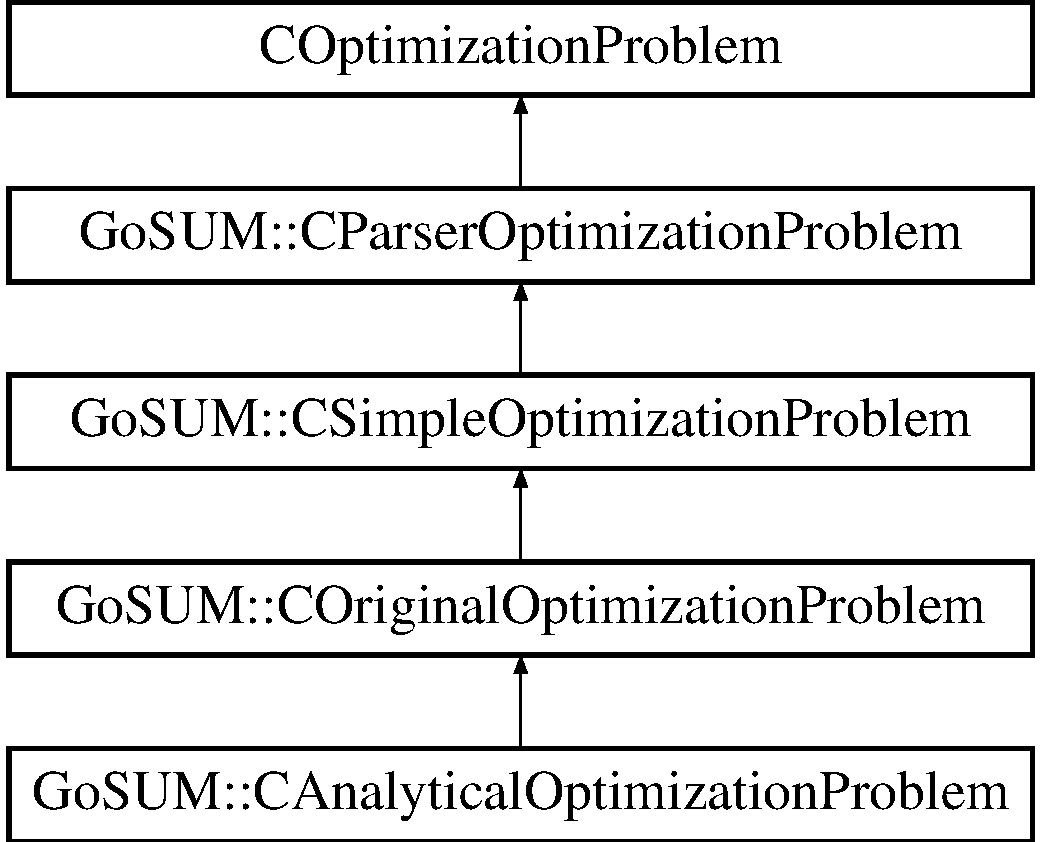
\includegraphics[height=5.000000cm]{class_go_s_u_m_1_1_c_analytical_optimization_problem}
\end{center}
\end{figure}
\subsection*{Public Member Functions}
\begin{DoxyCompactItemize}
\item 
\hyperlink{class_go_s_u_m_1_1_c_analytical_optimization_problem_a9bf7781536fcc8efc62d379aee03676f}{C\-Analytical\-Optimization\-Problem} (\hyperlink{class_go_s_u_m_1_1_c_input_parameters}{C\-Input\-Parameters} $\ast$\-\_\-p\-I\-P, \hyperlink{class_go_s_u_m_1_1_c_output_states}{C\-Output\-States} $\ast$\-\_\-p\-O\-S, \hyperlink{class_go_s_u_m_1_1_c_analytical_model}{C\-Analytical\-Model} $\ast$\-\_\-p\-A\-M)
\item 
virtual \hyperlink{class_go_s_u_m_1_1_c_analytical_optimization_problem_a5b6040cd5cf69ad24e076ce23152fedb}{$\sim$\-C\-Analytical\-Optimization\-Problem} ()
\item 
Array\-Xd \hyperlink{class_go_s_u_m_1_1_c_analytical_optimization_problem_a83cf54606759ec8e5cb20cbb0b0ce6f5}{input\-Point2\-Model\-Point} (const Array\-Xd \&\-\_\-ip)
\begin{DoxyCompactList}\small\item\em Converts input parameter point to model point. \end{DoxyCompactList}\end{DoxyCompactItemize}
\subsection*{Protected Member Functions}
\begin{DoxyCompactItemize}
\item 
{\footnotesize template$<$class Archive $>$ }\\void \hyperlink{class_go_s_u_m_1_1_c_analytical_optimization_problem_a258b0f6d24b501a1bb5ca1e65a06e8c5}{serialize} (Archive \&ar, const unsigned int version)
\item 
\hyperlink{class_go_s_u_m_1_1_c_analytical_optimization_problem_af6f91706b131e77c2b539b7e8965bbb1}{C\-Analytical\-Optimization\-Problem} ()
\end{DoxyCompactItemize}
\subsection*{Protected Attributes}
\begin{DoxyCompactItemize}
\item 
\hyperlink{class_go_s_u_m_1_1_c_analytical_model}{C\-Analytical\-Model} $\ast$ \hyperlink{class_go_s_u_m_1_1_c_analytical_optimization_problem_a31c65e8da1ad012c97e4c722120b0b0e}{p\-A\-M}
\end{DoxyCompactItemize}
\subsection*{Friends}
\begin{DoxyCompactItemize}
\item 
class \hyperlink{class_go_s_u_m_1_1_c_analytical_optimization_problem_ac98d07dd8f7b70e16ccb9a01abf56b9c}{boost\-::serialization\-::access}
\begin{DoxyCompactList}\small\item\em Boost serialization. \end{DoxyCompactList}\end{DoxyCompactItemize}
\subsection*{Additional Inherited Members}


\subsection{Detailed Description}
Class for the optimization problem based on \hyperlink{struct_go_s_u_m}{Go\-S\-U\-M} analyitical model. 

\subsection{Constructor \& Destructor Documentation}
\hypertarget{class_go_s_u_m_1_1_c_analytical_optimization_problem_af6f91706b131e77c2b539b7e8965bbb1}{\index{Go\-S\-U\-M\-::\-C\-Analytical\-Optimization\-Problem@{Go\-S\-U\-M\-::\-C\-Analytical\-Optimization\-Problem}!C\-Analytical\-Optimization\-Problem@{C\-Analytical\-Optimization\-Problem}}
\index{C\-Analytical\-Optimization\-Problem@{C\-Analytical\-Optimization\-Problem}!GoSUM::CAnalyticalOptimizationProblem@{Go\-S\-U\-M\-::\-C\-Analytical\-Optimization\-Problem}}
\subsubsection[{C\-Analytical\-Optimization\-Problem}]{\setlength{\rightskip}{0pt plus 5cm}Go\-S\-U\-M\-::\-C\-Analytical\-Optimization\-Problem\-::\-C\-Analytical\-Optimization\-Problem (
\begin{DoxyParamCaption}
{}
\end{DoxyParamCaption}
)\hspace{0.3cm}{\ttfamily [inline]}, {\ttfamily [protected]}}}\label{class_go_s_u_m_1_1_c_analytical_optimization_problem_af6f91706b131e77c2b539b7e8965bbb1}
\hypertarget{class_go_s_u_m_1_1_c_analytical_optimization_problem_a9bf7781536fcc8efc62d379aee03676f}{\index{Go\-S\-U\-M\-::\-C\-Analytical\-Optimization\-Problem@{Go\-S\-U\-M\-::\-C\-Analytical\-Optimization\-Problem}!C\-Analytical\-Optimization\-Problem@{C\-Analytical\-Optimization\-Problem}}
\index{C\-Analytical\-Optimization\-Problem@{C\-Analytical\-Optimization\-Problem}!GoSUM::CAnalyticalOptimizationProblem@{Go\-S\-U\-M\-::\-C\-Analytical\-Optimization\-Problem}}
\subsubsection[{C\-Analytical\-Optimization\-Problem}]{\setlength{\rightskip}{0pt plus 5cm}Go\-S\-U\-M\-::\-C\-Analytical\-Optimization\-Problem\-::\-C\-Analytical\-Optimization\-Problem (
\begin{DoxyParamCaption}
\item[{{\bf C\-Input\-Parameters} $\ast$}]{\-\_\-p\-I\-P, }
\item[{{\bf C\-Output\-States} $\ast$}]{\-\_\-p\-O\-S, }
\item[{{\bf C\-Analytical\-Model} $\ast$}]{\-\_\-p\-A\-M}
\end{DoxyParamCaption}
)\hspace{0.3cm}{\ttfamily [inline]}}}\label{class_go_s_u_m_1_1_c_analytical_optimization_problem_a9bf7781536fcc8efc62d379aee03676f}
\hypertarget{class_go_s_u_m_1_1_c_analytical_optimization_problem_a5b6040cd5cf69ad24e076ce23152fedb}{\index{Go\-S\-U\-M\-::\-C\-Analytical\-Optimization\-Problem@{Go\-S\-U\-M\-::\-C\-Analytical\-Optimization\-Problem}!$\sim$\-C\-Analytical\-Optimization\-Problem@{$\sim$\-C\-Analytical\-Optimization\-Problem}}
\index{$\sim$\-C\-Analytical\-Optimization\-Problem@{$\sim$\-C\-Analytical\-Optimization\-Problem}!GoSUM::CAnalyticalOptimizationProblem@{Go\-S\-U\-M\-::\-C\-Analytical\-Optimization\-Problem}}
\subsubsection[{$\sim$\-C\-Analytical\-Optimization\-Problem}]{\setlength{\rightskip}{0pt plus 5cm}virtual Go\-S\-U\-M\-::\-C\-Analytical\-Optimization\-Problem\-::$\sim$\-C\-Analytical\-Optimization\-Problem (
\begin{DoxyParamCaption}
{}
\end{DoxyParamCaption}
)\hspace{0.3cm}{\ttfamily [inline]}, {\ttfamily [virtual]}}}\label{class_go_s_u_m_1_1_c_analytical_optimization_problem_a5b6040cd5cf69ad24e076ce23152fedb}


\subsection{Member Function Documentation}
\hypertarget{class_go_s_u_m_1_1_c_analytical_optimization_problem_a83cf54606759ec8e5cb20cbb0b0ce6f5}{\index{Go\-S\-U\-M\-::\-C\-Analytical\-Optimization\-Problem@{Go\-S\-U\-M\-::\-C\-Analytical\-Optimization\-Problem}!input\-Point2\-Model\-Point@{input\-Point2\-Model\-Point}}
\index{input\-Point2\-Model\-Point@{input\-Point2\-Model\-Point}!GoSUM::CAnalyticalOptimizationProblem@{Go\-S\-U\-M\-::\-C\-Analytical\-Optimization\-Problem}}
\subsubsection[{input\-Point2\-Model\-Point}]{\setlength{\rightskip}{0pt plus 5cm}Array\-Xd Go\-S\-U\-M\-::\-C\-Analytical\-Optimization\-Problem\-::input\-Point2\-Model\-Point (
\begin{DoxyParamCaption}
\item[{const Array\-Xd \&}]{\-\_\-ip}
\end{DoxyParamCaption}
)}}\label{class_go_s_u_m_1_1_c_analytical_optimization_problem_a83cf54606759ec8e5cb20cbb0b0ce6f5}


Converts input parameter point to model point. 



Reimplemented from \hyperlink{class_go_s_u_m_1_1_c_original_optimization_problem_a3ad565122964e4fdec8156f6457c582e}{Go\-S\-U\-M\-::\-C\-Original\-Optimization\-Problem}.

\hypertarget{class_go_s_u_m_1_1_c_analytical_optimization_problem_a258b0f6d24b501a1bb5ca1e65a06e8c5}{\index{Go\-S\-U\-M\-::\-C\-Analytical\-Optimization\-Problem@{Go\-S\-U\-M\-::\-C\-Analytical\-Optimization\-Problem}!serialize@{serialize}}
\index{serialize@{serialize}!GoSUM::CAnalyticalOptimizationProblem@{Go\-S\-U\-M\-::\-C\-Analytical\-Optimization\-Problem}}
\subsubsection[{serialize}]{\setlength{\rightskip}{0pt plus 5cm}template$<$class Archive $>$ void Go\-S\-U\-M\-::\-C\-Analytical\-Optimization\-Problem\-::serialize (
\begin{DoxyParamCaption}
\item[{Archive \&}]{ar, }
\item[{const unsigned int}]{version}
\end{DoxyParamCaption}
)\hspace{0.3cm}{\ttfamily [protected]}}}\label{class_go_s_u_m_1_1_c_analytical_optimization_problem_a258b0f6d24b501a1bb5ca1e65a06e8c5}


Reimplemented from \hyperlink{class_go_s_u_m_1_1_c_original_optimization_problem_a41f4a21189b39fcdb0d820d2f8348475}{Go\-S\-U\-M\-::\-C\-Original\-Optimization\-Problem}.



\subsection{Friends And Related Function Documentation}
\hypertarget{class_go_s_u_m_1_1_c_analytical_optimization_problem_ac98d07dd8f7b70e16ccb9a01abf56b9c}{\index{Go\-S\-U\-M\-::\-C\-Analytical\-Optimization\-Problem@{Go\-S\-U\-M\-::\-C\-Analytical\-Optimization\-Problem}!boost\-::serialization\-::access@{boost\-::serialization\-::access}}
\index{boost\-::serialization\-::access@{boost\-::serialization\-::access}!GoSUM::CAnalyticalOptimizationProblem@{Go\-S\-U\-M\-::\-C\-Analytical\-Optimization\-Problem}}
\subsubsection[{boost\-::serialization\-::access}]{\setlength{\rightskip}{0pt plus 5cm}friend class boost\-::serialization\-::access\hspace{0.3cm}{\ttfamily [friend]}}}\label{class_go_s_u_m_1_1_c_analytical_optimization_problem_ac98d07dd8f7b70e16ccb9a01abf56b9c}


Boost serialization. 



\subsection{Member Data Documentation}
\hypertarget{class_go_s_u_m_1_1_c_analytical_optimization_problem_a31c65e8da1ad012c97e4c722120b0b0e}{\index{Go\-S\-U\-M\-::\-C\-Analytical\-Optimization\-Problem@{Go\-S\-U\-M\-::\-C\-Analytical\-Optimization\-Problem}!p\-A\-M@{p\-A\-M}}
\index{p\-A\-M@{p\-A\-M}!GoSUM::CAnalyticalOptimizationProblem@{Go\-S\-U\-M\-::\-C\-Analytical\-Optimization\-Problem}}
\subsubsection[{p\-A\-M}]{\setlength{\rightskip}{0pt plus 5cm}{\bf C\-Analytical\-Model}$\ast$ Go\-S\-U\-M\-::\-C\-Analytical\-Optimization\-Problem\-::p\-A\-M\hspace{0.3cm}{\ttfamily [protected]}}}\label{class_go_s_u_m_1_1_c_analytical_optimization_problem_a31c65e8da1ad012c97e4c722120b0b0e}
Points to analytical model. 

The documentation for this class was generated from the following files\-:\begin{DoxyCompactItemize}
\item 
C\-:/\-Development/core/\hyperlink{_parser_optimization_problem_8h}{Parser\-Optimization\-Problem.\-h}\item 
C\-:/\-Development/core/\hyperlink{_parser_optimization_problem_8cpp}{Parser\-Optimization\-Problem.\-cpp}\end{DoxyCompactItemize}

\hypertarget{class_c_base_r_n_g}{\section{C\-Base\-R\-N\-G Class Reference}
\label{class_c_base_r_n_g}\index{C\-Base\-R\-N\-G@{C\-Base\-R\-N\-G}}
}


Abstract base class for all uniform random number generators (R\-N\-G).  




{\ttfamily \#include $<$Random\-Generators.\-h$>$}

Inheritance diagram for C\-Base\-R\-N\-G\-:\begin{figure}[H]
\begin{center}
\leavevmode
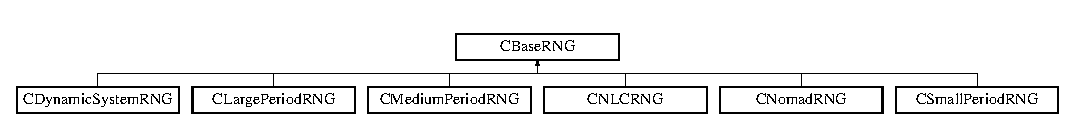
\includegraphics[height=1.296296cm]{class_c_base_r_n_g}
\end{center}
\end{figure}
\subsection*{Public Member Functions}
\begin{DoxyCompactItemize}
\item 
virtual void \hyperlink{class_c_base_r_n_g_a56fbf75ca07b73954596ee04820e0b07}{set\-Seed} (unsigned int s)=0
\begin{DoxyCompactList}\small\item\em Sets seed of the R\-N\-G. \end{DoxyCompactList}\item 
virtual unsigned int \hyperlink{class_c_base_r_n_g_a2db96fbf06a2f11b3613d422043fb7b8}{rndi} ()=0
\begin{DoxyCompactList}\small\item\em Returns randomly generated unsigned int. \end{DoxyCompactList}\item 
virtual double \hyperlink{class_c_base_r_n_g_abbd60a5ecdc9502dd646434224ab5d6b}{rnd} ()=0
\begin{DoxyCompactList}\small\item\em Returns randomly generated double between 0 and 1. \end{DoxyCompactList}\item 
virtual double \hyperlink{class_c_base_r_n_g_a5712044a0cd9fab6e60b914da7f35fc6}{rnd} (double a, double b)
\begin{DoxyCompactList}\small\item\em Returns randomly generated double between a and b. \end{DoxyCompactList}\end{DoxyCompactItemize}


\subsection{Detailed Description}
Abstract base class for all uniform random number generators (R\-N\-G). 

\subsection{Member Function Documentation}
\hypertarget{class_c_base_r_n_g_abbd60a5ecdc9502dd646434224ab5d6b}{\index{C\-Base\-R\-N\-G@{C\-Base\-R\-N\-G}!rnd@{rnd}}
\index{rnd@{rnd}!CBaseRNG@{C\-Base\-R\-N\-G}}
\subsubsection[{rnd}]{\setlength{\rightskip}{0pt plus 5cm}virtual double C\-Base\-R\-N\-G\-::rnd (
\begin{DoxyParamCaption}
{}
\end{DoxyParamCaption}
)\hspace{0.3cm}{\ttfamily [pure virtual]}}}\label{class_c_base_r_n_g_abbd60a5ecdc9502dd646434224ab5d6b}


Returns randomly generated double between 0 and 1. 



Implemented in \hyperlink{class_c_nomad_r_n_g_a80ec634087f50ef6753f1c5fe24c7ad4}{C\-Nomad\-R\-N\-G}, \hyperlink{class_c_n_l_c_r_n_g_a5f4f420ffb9147d9edb25b4d49ac05a5}{C\-N\-L\-C\-R\-N\-G}, \hyperlink{class_c_medium_period_r_n_g_a56a6e5751b8563b56c30f5c1d0351eec}{C\-Medium\-Period\-R\-N\-G}, \hyperlink{class_c_small_period_r_n_g_af82a1d5b0232cd7dc4b73114e632057c}{C\-Small\-Period\-R\-N\-G}, \hyperlink{class_c_dynamic_system_r_n_g_af22e28ce058d489e0b73b08033db87b8}{C\-Dynamic\-System\-R\-N\-G}, and \hyperlink{class_c_large_period_r_n_g_a3666cfacb7c24934e7f578ed2b786eb2}{C\-Large\-Period\-R\-N\-G}.

\hypertarget{class_c_base_r_n_g_a5712044a0cd9fab6e60b914da7f35fc6}{\index{C\-Base\-R\-N\-G@{C\-Base\-R\-N\-G}!rnd@{rnd}}
\index{rnd@{rnd}!CBaseRNG@{C\-Base\-R\-N\-G}}
\subsubsection[{rnd}]{\setlength{\rightskip}{0pt plus 5cm}virtual double C\-Base\-R\-N\-G\-::rnd (
\begin{DoxyParamCaption}
\item[{double}]{a, }
\item[{double}]{b}
\end{DoxyParamCaption}
)\hspace{0.3cm}{\ttfamily [inline]}, {\ttfamily [virtual]}}}\label{class_c_base_r_n_g_a5712044a0cd9fab6e60b914da7f35fc6}


Returns randomly generated double between a and b. 

\hypertarget{class_c_base_r_n_g_a2db96fbf06a2f11b3613d422043fb7b8}{\index{C\-Base\-R\-N\-G@{C\-Base\-R\-N\-G}!rndi@{rndi}}
\index{rndi@{rndi}!CBaseRNG@{C\-Base\-R\-N\-G}}
\subsubsection[{rndi}]{\setlength{\rightskip}{0pt plus 5cm}virtual unsigned int C\-Base\-R\-N\-G\-::rndi (
\begin{DoxyParamCaption}
{}
\end{DoxyParamCaption}
)\hspace{0.3cm}{\ttfamily [pure virtual]}}}\label{class_c_base_r_n_g_a2db96fbf06a2f11b3613d422043fb7b8}


Returns randomly generated unsigned int. 



Implemented in \hyperlink{class_c_nomad_r_n_g_ad41c27377065df6efdadc2d1b30ca315}{C\-Nomad\-R\-N\-G}, \hyperlink{class_c_n_l_c_r_n_g_a531b9ca98fc7934c90759c1733618298}{C\-N\-L\-C\-R\-N\-G}, \hyperlink{class_c_medium_period_r_n_g_a12611a6c74a312860cccfbdb2bdbf89e}{C\-Medium\-Period\-R\-N\-G}, \hyperlink{class_c_small_period_r_n_g_a60061ed8dc92ede13ad2a4579023e792}{C\-Small\-Period\-R\-N\-G}, \hyperlink{class_c_dynamic_system_r_n_g_a703c33a722eb6808771245955e19b3e1}{C\-Dynamic\-System\-R\-N\-G}, and \hyperlink{class_c_large_period_r_n_g_aadcf1849be317a7a4dc10500f168d8cd}{C\-Large\-Period\-R\-N\-G}.

\hypertarget{class_c_base_r_n_g_a56fbf75ca07b73954596ee04820e0b07}{\index{C\-Base\-R\-N\-G@{C\-Base\-R\-N\-G}!set\-Seed@{set\-Seed}}
\index{set\-Seed@{set\-Seed}!CBaseRNG@{C\-Base\-R\-N\-G}}
\subsubsection[{set\-Seed}]{\setlength{\rightskip}{0pt plus 5cm}virtual void C\-Base\-R\-N\-G\-::set\-Seed (
\begin{DoxyParamCaption}
\item[{unsigned int}]{s}
\end{DoxyParamCaption}
)\hspace{0.3cm}{\ttfamily [pure virtual]}}}\label{class_c_base_r_n_g_a56fbf75ca07b73954596ee04820e0b07}


Sets seed of the R\-N\-G. 



Implemented in \hyperlink{class_c_nomad_r_n_g_a6cedb9431179cee4677d415c8e7611c3}{C\-Nomad\-R\-N\-G}, \hyperlink{class_c_n_l_c_r_n_g_a9f6321c4d53774b0c017c6e18124d495}{C\-N\-L\-C\-R\-N\-G}, \hyperlink{class_c_medium_period_r_n_g_a8f0a3aebcea30b879719d9af1ac548e1}{C\-Medium\-Period\-R\-N\-G}, \hyperlink{class_c_small_period_r_n_g_a7a799121f858fd32c8300970ab46a26a}{C\-Small\-Period\-R\-N\-G}, \hyperlink{class_c_dynamic_system_r_n_g_a2ed468a45094e3c0591e0029b1359df1}{C\-Dynamic\-System\-R\-N\-G}, and \hyperlink{class_c_large_period_r_n_g_a59d03465a293ce805a34339f409054d7}{C\-Large\-Period\-R\-N\-G}.



The documentation for this class was generated from the following file\-:\begin{DoxyCompactItemize}
\item 
C\-:/\-Development/core/\hyperlink{_random_generators_8h}{Random\-Generators.\-h}\end{DoxyCompactItemize}

\hypertarget{class_c_categorical_d_r_v}{\section{C\-Categorical\-D\-R\-V Class Reference}
\label{class_c_categorical_d_r_v}\index{C\-Categorical\-D\-R\-V@{C\-Categorical\-D\-R\-V}}
}


Class for categorical discrete random variables derived from discrete random variables.  




{\ttfamily \#include $<$Random\-Variable.\-h$>$}

Inheritance diagram for C\-Categorical\-D\-R\-V\-:\begin{figure}[H]
\begin{center}
\leavevmode
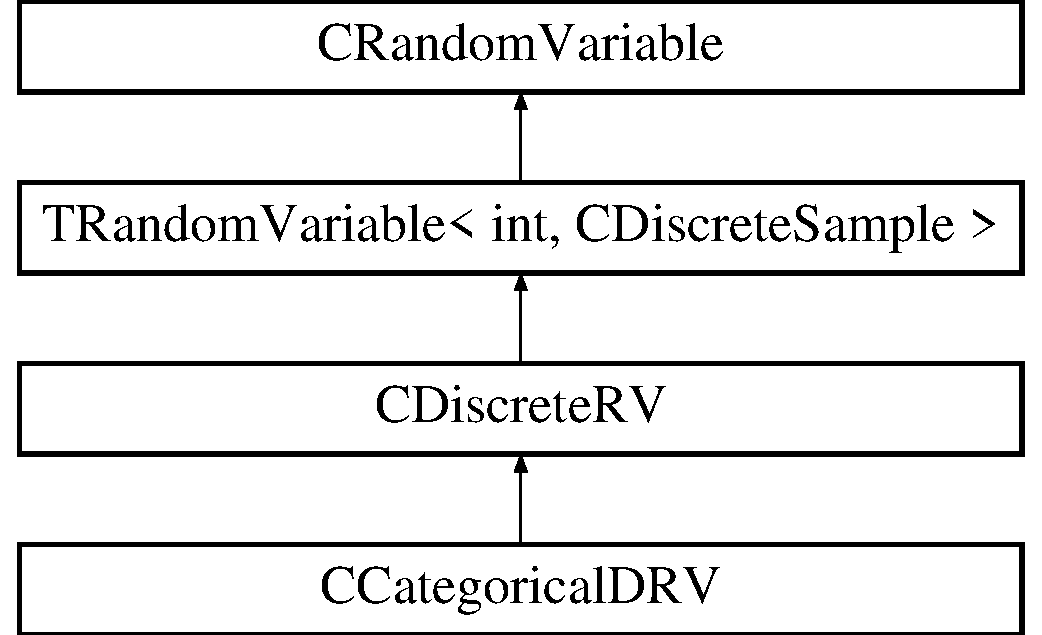
\includegraphics[height=4.000000cm]{class_c_categorical_d_r_v}
\end{center}
\end{figure}
\subsection*{Public Member Functions}
\begin{DoxyCompactItemize}
\item 
\hyperlink{class_c_categorical_d_r_v_a4fec729c76cfbfb22e19ed4a47b3d8f6}{C\-Categorical\-D\-R\-V} ()
\item 
virtual \hyperlink{class_c_categorical_d_r_v_a3e3e653c5b11c99ab6c9ad352cd1a5ee}{$\sim$\-C\-Categorical\-D\-R\-V} ()
\item 
\hyperlink{class_c_categorical_d_r_v_afec3ee33d70f726e48c2cfeff9644196}{C\-Categorical\-D\-R\-V} (const \hyperlink{class_c_categorical_d_r_v}{C\-Categorical\-D\-R\-V} \&O)
\item 
virtual void \hyperlink{class_c_categorical_d_r_v_aba3393786eddeb6a235cd1e58d88c280}{set\-Distribution} (const \hyperlink{class_c_discrete_sample}{C\-Discrete\-Sample} \&\-\_\-a\-S)
\begin{DoxyCompactList}\small\item\em Computes P\-M\-F and C\-D\-F from sample histogram. \end{DoxyCompactList}\item 
virtual double \hyperlink{class_c_categorical_d_r_v_a7bbfb60b24d3aa7ef4aaa42212eeb638}{probability} (int \-\_\-k) const 
\begin{DoxyCompactList}\small\item\em Function that returns P\-M\-F. \end{DoxyCompactList}\item 
virtual double \hyperlink{class_c_categorical_d_r_v_a65d62077439f102b8e68a98e32a71df5}{cumulative} (int \-\_\-k) const 
\begin{DoxyCompactList}\small\item\em Function that returns C\-D\-F. \end{DoxyCompactList}\item 
virtual int \hyperlink{class_c_categorical_d_r_v_a385ff0c56ffc1c32b57f6b73ec4e1b79}{expanded\-Size} () const 
\item 
virtual double \hyperlink{class_c_categorical_d_r_v_a2b4cfded808f058c38d931ac4c74ad31}{min\-Value} () const 
\begin{DoxyCompactList}\small\item\em After expansion, number of new variables is equal to the number of categories. \end{DoxyCompactList}\item 
virtual double \hyperlink{class_c_categorical_d_r_v_aa5d047a29e2ff173134e60a04f24eb1c}{max\-Value} () const 
\begin{DoxyCompactList}\small\item\em Returns maximal value of the random variable. \end{DoxyCompactList}\item 
virtual double \hyperlink{class_c_categorical_d_r_v_ad771cb6295a706cf14e666ab097d4751}{expected\-Value} () const 
\begin{DoxyCompactList}\small\item\em Returns expected value of the random variable. \end{DoxyCompactList}\item 
virtual \hyperlink{class_c_random_variable_a80d2a87c43847274138b51f7d713d7f1}{distributiontype} \hyperlink{class_c_categorical_d_r_v_affe36486c2cc2b8b35018bd0557cf4d4}{distribution\-Type} () const 
\begin{DoxyCompactList}\small\item\em Returns enum type of the random variable distribution. \end{DoxyCompactList}\item 
virtual std\-::string \hyperlink{class_c_categorical_d_r_v_adbecb8ad887cdbe9c1f39858c415e70a}{distribution\-Name} () const 
\begin{DoxyCompactList}\small\item\em Returns name of the random variable distribution. \end{DoxyCompactList}\item 
virtual Array\-Xi \hyperlink{class_c_categorical_d_r_v_a67bb1a1664827e7221af1178b78c7850}{export\-Domain} () const 
\begin{DoxyCompactList}\small\item\em Exports domain of the random variable. \end{DoxyCompactList}\item 
virtual bool \hyperlink{class_c_categorical_d_r_v_a43881a5705bc5c0de35488ca13fb31e6}{is\-Distribution\-Defined} () const 
\begin{DoxyCompactList}\small\item\em Returns true if distribution is defined, false otherwise. \end{DoxyCompactList}\item 
virtual double \hyperlink{class_c_categorical_d_r_v_a78e27950e4b4e248abd75305b55d0519}{variance} () const 
\begin{DoxyCompactList}\small\item\em Returns variance of the random variable. \end{DoxyCompactList}\end{DoxyCompactItemize}
\subsection*{Protected Member Functions}
\begin{DoxyCompactItemize}
\item 
virtual double \hyperlink{class_c_categorical_d_r_v_ad13850307d82f7d771a8e658305f2083}{do\-Quantile} (double \-\_\-p) const 
\begin{DoxyCompactList}\small\item\em Quantile, formula implementation. \end{DoxyCompactList}\end{DoxyCompactItemize}
\subsection*{Private Member Functions}
\begin{DoxyCompactItemize}
\item 
{\footnotesize template$<$class Archive $>$ }\\void \hyperlink{class_c_categorical_d_r_v_a7d834148a34cfdabdb71040858032fcf}{serialize} (Archive \&ar, const unsigned int version)
\end{DoxyCompactItemize}
\subsection*{Private Attributes}
\begin{DoxyCompactItemize}
\item 
Array\-Xd \hyperlink{class_c_categorical_d_r_v_ae7de998dd49975a1be0de37cbc4f23b5}{p}
\item 
Array\-Xd \hyperlink{class_c_categorical_d_r_v_a78c2837dfae368a3ecdbb416b0e9d094}{cdf}
\end{DoxyCompactItemize}
\subsection*{Friends}
\begin{DoxyCompactItemize}
\item 
class \hyperlink{class_c_categorical_d_r_v_ac98d07dd8f7b70e16ccb9a01abf56b9c}{boost\-::serialization\-::access}
\begin{DoxyCompactList}\small\item\em Boost serialization. \end{DoxyCompactList}\end{DoxyCompactItemize}
\subsection*{Additional Inherited Members}


\subsection{Detailed Description}
Class for categorical discrete random variables derived from discrete random variables. 

\subsection{Constructor \& Destructor Documentation}
\hypertarget{class_c_categorical_d_r_v_a4fec729c76cfbfb22e19ed4a47b3d8f6}{\index{C\-Categorical\-D\-R\-V@{C\-Categorical\-D\-R\-V}!C\-Categorical\-D\-R\-V@{C\-Categorical\-D\-R\-V}}
\index{C\-Categorical\-D\-R\-V@{C\-Categorical\-D\-R\-V}!CCategoricalDRV@{C\-Categorical\-D\-R\-V}}
\subsubsection[{C\-Categorical\-D\-R\-V}]{\setlength{\rightskip}{0pt plus 5cm}C\-Categorical\-D\-R\-V\-::\-C\-Categorical\-D\-R\-V (
\begin{DoxyParamCaption}
{}
\end{DoxyParamCaption}
)\hspace{0.3cm}{\ttfamily [inline]}}}\label{class_c_categorical_d_r_v_a4fec729c76cfbfb22e19ed4a47b3d8f6}
\hypertarget{class_c_categorical_d_r_v_a3e3e653c5b11c99ab6c9ad352cd1a5ee}{\index{C\-Categorical\-D\-R\-V@{C\-Categorical\-D\-R\-V}!$\sim$\-C\-Categorical\-D\-R\-V@{$\sim$\-C\-Categorical\-D\-R\-V}}
\index{$\sim$\-C\-Categorical\-D\-R\-V@{$\sim$\-C\-Categorical\-D\-R\-V}!CCategoricalDRV@{C\-Categorical\-D\-R\-V}}
\subsubsection[{$\sim$\-C\-Categorical\-D\-R\-V}]{\setlength{\rightskip}{0pt plus 5cm}virtual C\-Categorical\-D\-R\-V\-::$\sim$\-C\-Categorical\-D\-R\-V (
\begin{DoxyParamCaption}
{}
\end{DoxyParamCaption}
)\hspace{0.3cm}{\ttfamily [inline]}, {\ttfamily [virtual]}}}\label{class_c_categorical_d_r_v_a3e3e653c5b11c99ab6c9ad352cd1a5ee}
\hypertarget{class_c_categorical_d_r_v_afec3ee33d70f726e48c2cfeff9644196}{\index{C\-Categorical\-D\-R\-V@{C\-Categorical\-D\-R\-V}!C\-Categorical\-D\-R\-V@{C\-Categorical\-D\-R\-V}}
\index{C\-Categorical\-D\-R\-V@{C\-Categorical\-D\-R\-V}!CCategoricalDRV@{C\-Categorical\-D\-R\-V}}
\subsubsection[{C\-Categorical\-D\-R\-V}]{\setlength{\rightskip}{0pt plus 5cm}C\-Categorical\-D\-R\-V\-::\-C\-Categorical\-D\-R\-V (
\begin{DoxyParamCaption}
\item[{const {\bf C\-Categorical\-D\-R\-V} \&}]{O}
\end{DoxyParamCaption}
)\hspace{0.3cm}{\ttfamily [inline]}}}\label{class_c_categorical_d_r_v_afec3ee33d70f726e48c2cfeff9644196}


\subsection{Member Function Documentation}
\hypertarget{class_c_categorical_d_r_v_a65d62077439f102b8e68a98e32a71df5}{\index{C\-Categorical\-D\-R\-V@{C\-Categorical\-D\-R\-V}!cumulative@{cumulative}}
\index{cumulative@{cumulative}!CCategoricalDRV@{C\-Categorical\-D\-R\-V}}
\subsubsection[{cumulative}]{\setlength{\rightskip}{0pt plus 5cm}virtual double C\-Categorical\-D\-R\-V\-::cumulative (
\begin{DoxyParamCaption}
\item[{int}]{\-\_\-k}
\end{DoxyParamCaption}
) const\hspace{0.3cm}{\ttfamily [inline]}, {\ttfamily [virtual]}}}\label{class_c_categorical_d_r_v_a65d62077439f102b8e68a98e32a71df5}


Function that returns C\-D\-F. 

\hypertarget{class_c_categorical_d_r_v_adbecb8ad887cdbe9c1f39858c415e70a}{\index{C\-Categorical\-D\-R\-V@{C\-Categorical\-D\-R\-V}!distribution\-Name@{distribution\-Name}}
\index{distribution\-Name@{distribution\-Name}!CCategoricalDRV@{C\-Categorical\-D\-R\-V}}
\subsubsection[{distribution\-Name}]{\setlength{\rightskip}{0pt plus 5cm}virtual std\-::string C\-Categorical\-D\-R\-V\-::distribution\-Name (
\begin{DoxyParamCaption}
{}
\end{DoxyParamCaption}
) const\hspace{0.3cm}{\ttfamily [inline]}, {\ttfamily [virtual]}}}\label{class_c_categorical_d_r_v_adbecb8ad887cdbe9c1f39858c415e70a}


Returns name of the random variable distribution. 



Implements \hyperlink{class_c_random_variable_a4b33eef7c56f9f1a83af01fa8ef2502b}{C\-Random\-Variable}.

\hypertarget{class_c_categorical_d_r_v_affe36486c2cc2b8b35018bd0557cf4d4}{\index{C\-Categorical\-D\-R\-V@{C\-Categorical\-D\-R\-V}!distribution\-Type@{distribution\-Type}}
\index{distribution\-Type@{distribution\-Type}!CCategoricalDRV@{C\-Categorical\-D\-R\-V}}
\subsubsection[{distribution\-Type}]{\setlength{\rightskip}{0pt plus 5cm}virtual {\bf distributiontype} C\-Categorical\-D\-R\-V\-::distribution\-Type (
\begin{DoxyParamCaption}
{}
\end{DoxyParamCaption}
) const\hspace{0.3cm}{\ttfamily [inline]}, {\ttfamily [virtual]}}}\label{class_c_categorical_d_r_v_affe36486c2cc2b8b35018bd0557cf4d4}


Returns enum type of the random variable distribution. 



Implements \hyperlink{class_c_random_variable_a3b30589d41f4dd200bd40c8273cac2cd}{C\-Random\-Variable}.

\hypertarget{class_c_categorical_d_r_v_ad13850307d82f7d771a8e658305f2083}{\index{C\-Categorical\-D\-R\-V@{C\-Categorical\-D\-R\-V}!do\-Quantile@{do\-Quantile}}
\index{do\-Quantile@{do\-Quantile}!CCategoricalDRV@{C\-Categorical\-D\-R\-V}}
\subsubsection[{do\-Quantile}]{\setlength{\rightskip}{0pt plus 5cm}double C\-Categorical\-D\-R\-V\-::do\-Quantile (
\begin{DoxyParamCaption}
\item[{double}]{\-\_\-p}
\end{DoxyParamCaption}
) const\hspace{0.3cm}{\ttfamily [protected]}, {\ttfamily [virtual]}}}\label{class_c_categorical_d_r_v_ad13850307d82f7d771a8e658305f2083}


Quantile, formula implementation. 



Implements \hyperlink{class_c_random_variable_a552ab36c8144d7154cbe3cd363eee65b}{C\-Random\-Variable}.

\hypertarget{class_c_categorical_d_r_v_a385ff0c56ffc1c32b57f6b73ec4e1b79}{\index{C\-Categorical\-D\-R\-V@{C\-Categorical\-D\-R\-V}!expanded\-Size@{expanded\-Size}}
\index{expanded\-Size@{expanded\-Size}!CCategoricalDRV@{C\-Categorical\-D\-R\-V}}
\subsubsection[{expanded\-Size}]{\setlength{\rightskip}{0pt plus 5cm}virtual int C\-Categorical\-D\-R\-V\-::expanded\-Size (
\begin{DoxyParamCaption}
{}
\end{DoxyParamCaption}
) const\hspace{0.3cm}{\ttfamily [inline]}, {\ttfamily [virtual]}}}\label{class_c_categorical_d_r_v_a385ff0c56ffc1c32b57f6b73ec4e1b79}


Reimplemented from \hyperlink{class_c_random_variable_ada091c2895cf25a75ac8aacecb5da47f}{C\-Random\-Variable}.

\hypertarget{class_c_categorical_d_r_v_ad771cb6295a706cf14e666ab097d4751}{\index{C\-Categorical\-D\-R\-V@{C\-Categorical\-D\-R\-V}!expected\-Value@{expected\-Value}}
\index{expected\-Value@{expected\-Value}!CCategoricalDRV@{C\-Categorical\-D\-R\-V}}
\subsubsection[{expected\-Value}]{\setlength{\rightskip}{0pt plus 5cm}virtual double C\-Categorical\-D\-R\-V\-::expected\-Value (
\begin{DoxyParamCaption}
{}
\end{DoxyParamCaption}
) const\hspace{0.3cm}{\ttfamily [inline]}, {\ttfamily [virtual]}}}\label{class_c_categorical_d_r_v_ad771cb6295a706cf14e666ab097d4751}


Returns expected value of the random variable. 



Implements \hyperlink{class_c_random_variable_a6e5490d17f2b6abcf9922c8b1bd6d4ed}{C\-Random\-Variable}.

\hypertarget{class_c_categorical_d_r_v_a67bb1a1664827e7221af1178b78c7850}{\index{C\-Categorical\-D\-R\-V@{C\-Categorical\-D\-R\-V}!export\-Domain@{export\-Domain}}
\index{export\-Domain@{export\-Domain}!CCategoricalDRV@{C\-Categorical\-D\-R\-V}}
\subsubsection[{export\-Domain}]{\setlength{\rightskip}{0pt plus 5cm}Array\-Xi C\-Categorical\-D\-R\-V\-::export\-Domain (
\begin{DoxyParamCaption}
{}
\end{DoxyParamCaption}
) const\hspace{0.3cm}{\ttfamily [virtual]}}}\label{class_c_categorical_d_r_v_a67bb1a1664827e7221af1178b78c7850}


Exports domain of the random variable. 



Implements \hyperlink{class_t_random_variable_a37fc52d5fa37493a353887242d279a27}{T\-Random\-Variable$<$ t, T $>$}.

\hypertarget{class_c_categorical_d_r_v_a43881a5705bc5c0de35488ca13fb31e6}{\index{C\-Categorical\-D\-R\-V@{C\-Categorical\-D\-R\-V}!is\-Distribution\-Defined@{is\-Distribution\-Defined}}
\index{is\-Distribution\-Defined@{is\-Distribution\-Defined}!CCategoricalDRV@{C\-Categorical\-D\-R\-V}}
\subsubsection[{is\-Distribution\-Defined}]{\setlength{\rightskip}{0pt plus 5cm}virtual bool C\-Categorical\-D\-R\-V\-::is\-Distribution\-Defined (
\begin{DoxyParamCaption}
{}
\end{DoxyParamCaption}
) const\hspace{0.3cm}{\ttfamily [inline]}, {\ttfamily [virtual]}}}\label{class_c_categorical_d_r_v_a43881a5705bc5c0de35488ca13fb31e6}


Returns true if distribution is defined, false otherwise. 



Reimplemented from \hyperlink{class_c_random_variable_a60e88c15450ab21dea6bef00d8836da7}{C\-Random\-Variable}.

\hypertarget{class_c_categorical_d_r_v_aa5d047a29e2ff173134e60a04f24eb1c}{\index{C\-Categorical\-D\-R\-V@{C\-Categorical\-D\-R\-V}!max\-Value@{max\-Value}}
\index{max\-Value@{max\-Value}!CCategoricalDRV@{C\-Categorical\-D\-R\-V}}
\subsubsection[{max\-Value}]{\setlength{\rightskip}{0pt plus 5cm}virtual double C\-Categorical\-D\-R\-V\-::max\-Value (
\begin{DoxyParamCaption}
{}
\end{DoxyParamCaption}
) const\hspace{0.3cm}{\ttfamily [inline]}, {\ttfamily [virtual]}}}\label{class_c_categorical_d_r_v_aa5d047a29e2ff173134e60a04f24eb1c}


Returns maximal value of the random variable. 



Implements \hyperlink{class_c_random_variable_a48a5e98363d866f1f46568ed658479ad}{C\-Random\-Variable}.

\hypertarget{class_c_categorical_d_r_v_a2b4cfded808f058c38d931ac4c74ad31}{\index{C\-Categorical\-D\-R\-V@{C\-Categorical\-D\-R\-V}!min\-Value@{min\-Value}}
\index{min\-Value@{min\-Value}!CCategoricalDRV@{C\-Categorical\-D\-R\-V}}
\subsubsection[{min\-Value}]{\setlength{\rightskip}{0pt plus 5cm}virtual double C\-Categorical\-D\-R\-V\-::min\-Value (
\begin{DoxyParamCaption}
{}
\end{DoxyParamCaption}
) const\hspace{0.3cm}{\ttfamily [inline]}, {\ttfamily [virtual]}}}\label{class_c_categorical_d_r_v_a2b4cfded808f058c38d931ac4c74ad31}


After expansion, number of new variables is equal to the number of categories. 

Returns minimal value of the random variable. 

Implements \hyperlink{class_c_random_variable_a233ddd2eedb51b09a04a8c330646f356}{C\-Random\-Variable}.

\hypertarget{class_c_categorical_d_r_v_a7bbfb60b24d3aa7ef4aaa42212eeb638}{\index{C\-Categorical\-D\-R\-V@{C\-Categorical\-D\-R\-V}!probability@{probability}}
\index{probability@{probability}!CCategoricalDRV@{C\-Categorical\-D\-R\-V}}
\subsubsection[{probability}]{\setlength{\rightskip}{0pt plus 5cm}virtual double C\-Categorical\-D\-R\-V\-::probability (
\begin{DoxyParamCaption}
\item[{int}]{\-\_\-k}
\end{DoxyParamCaption}
) const\hspace{0.3cm}{\ttfamily [inline]}, {\ttfamily [virtual]}}}\label{class_c_categorical_d_r_v_a7bbfb60b24d3aa7ef4aaa42212eeb638}


Function that returns P\-M\-F. 

\hypertarget{class_c_categorical_d_r_v_a7d834148a34cfdabdb71040858032fcf}{\index{C\-Categorical\-D\-R\-V@{C\-Categorical\-D\-R\-V}!serialize@{serialize}}
\index{serialize@{serialize}!CCategoricalDRV@{C\-Categorical\-D\-R\-V}}
\subsubsection[{serialize}]{\setlength{\rightskip}{0pt plus 5cm}template$<$class Archive $>$ void C\-Categorical\-D\-R\-V\-::serialize (
\begin{DoxyParamCaption}
\item[{Archive \&}]{ar, }
\item[{const unsigned int}]{version}
\end{DoxyParamCaption}
)\hspace{0.3cm}{\ttfamily [private]}}}\label{class_c_categorical_d_r_v_a7d834148a34cfdabdb71040858032fcf}
\hypertarget{class_c_categorical_d_r_v_aba3393786eddeb6a235cd1e58d88c280}{\index{C\-Categorical\-D\-R\-V@{C\-Categorical\-D\-R\-V}!set\-Distribution@{set\-Distribution}}
\index{set\-Distribution@{set\-Distribution}!CCategoricalDRV@{C\-Categorical\-D\-R\-V}}
\subsubsection[{set\-Distribution}]{\setlength{\rightskip}{0pt plus 5cm}void C\-Categorical\-D\-R\-V\-::set\-Distribution (
\begin{DoxyParamCaption}
\item[{const {\bf C\-Discrete\-Sample} \&}]{\-\_\-a\-S}
\end{DoxyParamCaption}
)\hspace{0.3cm}{\ttfamily [virtual]}}}\label{class_c_categorical_d_r_v_aba3393786eddeb6a235cd1e58d88c280}


Computes P\-M\-F and C\-D\-F from sample histogram. 

\hypertarget{class_c_categorical_d_r_v_a78e27950e4b4e248abd75305b55d0519}{\index{C\-Categorical\-D\-R\-V@{C\-Categorical\-D\-R\-V}!variance@{variance}}
\index{variance@{variance}!CCategoricalDRV@{C\-Categorical\-D\-R\-V}}
\subsubsection[{variance}]{\setlength{\rightskip}{0pt plus 5cm}virtual double C\-Categorical\-D\-R\-V\-::variance (
\begin{DoxyParamCaption}
{}
\end{DoxyParamCaption}
) const\hspace{0.3cm}{\ttfamily [inline]}, {\ttfamily [virtual]}}}\label{class_c_categorical_d_r_v_a78e27950e4b4e248abd75305b55d0519}


Returns variance of the random variable. 



Implements \hyperlink{class_c_random_variable_a3b0b87c4aab74c0406cd8321b8b96747}{C\-Random\-Variable}.



\subsection{Friends And Related Function Documentation}
\hypertarget{class_c_categorical_d_r_v_ac98d07dd8f7b70e16ccb9a01abf56b9c}{\index{C\-Categorical\-D\-R\-V@{C\-Categorical\-D\-R\-V}!boost\-::serialization\-::access@{boost\-::serialization\-::access}}
\index{boost\-::serialization\-::access@{boost\-::serialization\-::access}!CCategoricalDRV@{C\-Categorical\-D\-R\-V}}
\subsubsection[{boost\-::serialization\-::access}]{\setlength{\rightskip}{0pt plus 5cm}friend class boost\-::serialization\-::access\hspace{0.3cm}{\ttfamily [friend]}}}\label{class_c_categorical_d_r_v_ac98d07dd8f7b70e16ccb9a01abf56b9c}


Boost serialization. 



\subsection{Member Data Documentation}
\hypertarget{class_c_categorical_d_r_v_a78c2837dfae368a3ecdbb416b0e9d094}{\index{C\-Categorical\-D\-R\-V@{C\-Categorical\-D\-R\-V}!cdf@{cdf}}
\index{cdf@{cdf}!CCategoricalDRV@{C\-Categorical\-D\-R\-V}}
\subsubsection[{cdf}]{\setlength{\rightskip}{0pt plus 5cm}Array\-Xd C\-Categorical\-D\-R\-V\-::cdf\hspace{0.3cm}{\ttfamily [private]}}}\label{class_c_categorical_d_r_v_a78c2837dfae368a3ecdbb416b0e9d094}
P\-M\-F (p) and C\-D\-F (cdf) data. \hypertarget{class_c_categorical_d_r_v_ae7de998dd49975a1be0de37cbc4f23b5}{\index{C\-Categorical\-D\-R\-V@{C\-Categorical\-D\-R\-V}!p@{p}}
\index{p@{p}!CCategoricalDRV@{C\-Categorical\-D\-R\-V}}
\subsubsection[{p}]{\setlength{\rightskip}{0pt plus 5cm}Array\-Xd C\-Categorical\-D\-R\-V\-::p\hspace{0.3cm}{\ttfamily [private]}}}\label{class_c_categorical_d_r_v_ae7de998dd49975a1be0de37cbc4f23b5}


The documentation for this class was generated from the following files\-:\begin{DoxyCompactItemize}
\item 
C\-:/\-Development/core/\hyperlink{_random_variable_8h}{Random\-Variable.\-h}\item 
C\-:/\-Development/core/\hyperlink{_random_variable_8cpp}{Random\-Variable.\-cpp}\end{DoxyCompactItemize}

\hypertarget{class_c_categorical_sample}{\section{C\-Categorical\-Sample Class Reference}
\label{class_c_categorical_sample}\index{C\-Categorical\-Sample@{C\-Categorical\-Sample}}
}


Abstract class for categorical discrete samples.  




{\ttfamily \#include $<$Sample.\-h$>$}

Inheritance diagram for C\-Categorical\-Sample\-:\begin{figure}[H]
\begin{center}
\leavevmode
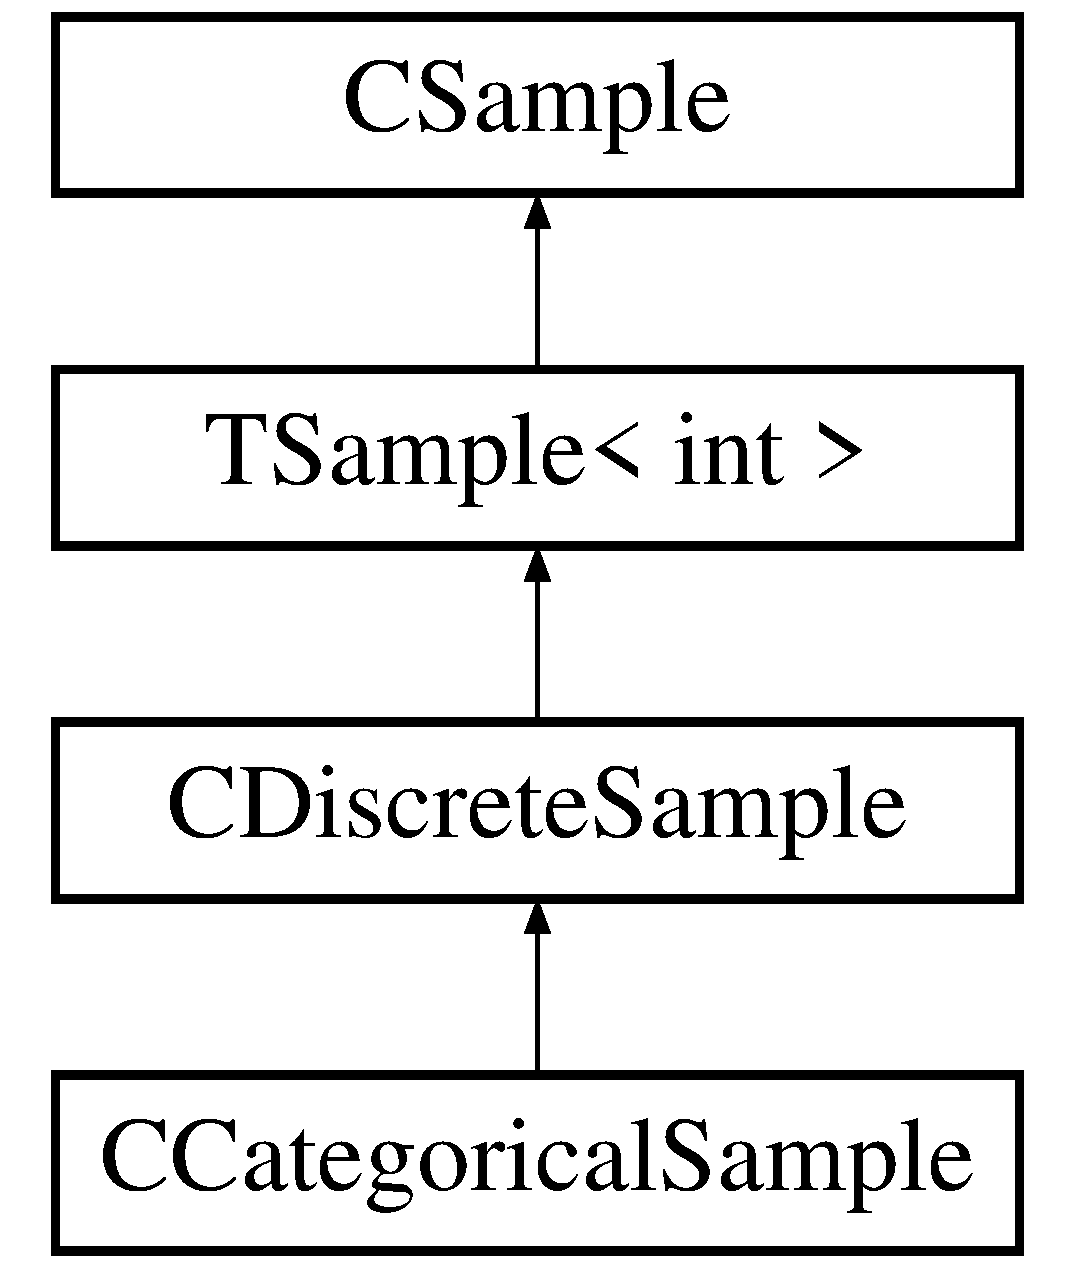
\includegraphics[height=4.000000cm]{class_c_categorical_sample}
\end{center}
\end{figure}
\subsection*{Public Member Functions}
\begin{DoxyCompactItemize}
\item 
\hyperlink{class_c_categorical_sample_aab6ec20d09a316f730afc171537a7713}{C\-Categorical\-Sample} ()
\item 
\hyperlink{class_c_categorical_sample_ab66a69b33d8ca70fe3bb13c65d502054}{C\-Categorical\-Sample} (const \hyperlink{class_c_categorical_sample}{C\-Categorical\-Sample} \&O)
\item 
virtual \hyperlink{class_c_categorical_sample_a65c4e0faf826db2641f2d18e04a1fb4c}{$\sim$\-C\-Categorical\-Sample} ()
\item 
virtual void \hyperlink{class_c_categorical_sample_af1adebf697521884fdc51653ee5f4b97}{read\-Sample\-Value} (std\-::ifstream \&\-\_\-ifs, int \-\_\-at)
\begin{DoxyCompactList}\small\item\em Reads particular sample data from input file stream. \end{DoxyCompactList}\item 
virtual void \hyperlink{class_c_categorical_sample_ab20e228cf0a5b43de4981e1cc95da129}{write\-Sample\-Value} (std\-::ofstream \&\-\_\-ofs, int \-\_\-at) const 
\begin{DoxyCompactList}\small\item\em $<$ Writes particular sample data to output file stream. \end{DoxyCompactList}\item 
virtual void \hyperlink{class_c_categorical_sample_a7326fb12831014e2ee7504eb010f6356}{set\-Sample\-Size} (int \-\_\-n)
\begin{DoxyCompactList}\small\item\em Sets particular sample data value. \end{DoxyCompactList}\item 
int \hyperlink{class_c_categorical_sample_a4c14022735a64792701f670a6d6d38e6}{min\-Value} () const 
\begin{DoxyCompactList}\small\item\em Returns minimal sample data value. \end{DoxyCompactList}\item 
int \hyperlink{class_c_categorical_sample_a26021cff1304912e26023cddc399b67e}{max\-Value} () const 
\begin{DoxyCompactList}\small\item\em Returns maximal sample data value. \end{DoxyCompactList}\item 
virtual double \hyperlink{class_c_categorical_sample_a5408236fafb24d5a246823b97cc7427a}{variance} () const 
\begin{DoxyCompactList}\small\item\em Returns sample variance (i.\-e.\-empirical). \end{DoxyCompactList}\end{DoxyCompactItemize}
\subsection*{Private Member Functions}
\begin{DoxyCompactItemize}
\item 
{\footnotesize template$<$class Archive $>$ }\\void \hyperlink{class_c_categorical_sample_a7f4ae293dfb2f77bd6d9b525f1e9cbf1}{serialize} (Archive \&ar, const unsigned int version)
\end{DoxyCompactItemize}
\subsection*{Private Attributes}
\begin{DoxyCompactItemize}
\item 
std\-::vector$<$ std\-::string $>$ \hyperlink{class_c_categorical_sample_ae713b59c14aba1434e1754d837a4eeb0}{categories}
\end{DoxyCompactItemize}
\subsection*{Friends}
\begin{DoxyCompactItemize}
\item 
class \hyperlink{class_c_categorical_sample_ac98d07dd8f7b70e16ccb9a01abf56b9c}{boost\-::serialization\-::access}
\begin{DoxyCompactList}\small\item\em Boost serialization. \end{DoxyCompactList}\end{DoxyCompactItemize}
\subsection*{Additional Inherited Members}


\subsection{Detailed Description}
Abstract class for categorical discrete samples. 

\subsection{Constructor \& Destructor Documentation}
\hypertarget{class_c_categorical_sample_aab6ec20d09a316f730afc171537a7713}{\index{C\-Categorical\-Sample@{C\-Categorical\-Sample}!C\-Categorical\-Sample@{C\-Categorical\-Sample}}
\index{C\-Categorical\-Sample@{C\-Categorical\-Sample}!CCategoricalSample@{C\-Categorical\-Sample}}
\subsubsection[{C\-Categorical\-Sample}]{\setlength{\rightskip}{0pt plus 5cm}C\-Categorical\-Sample\-::\-C\-Categorical\-Sample (
\begin{DoxyParamCaption}
{}
\end{DoxyParamCaption}
)\hspace{0.3cm}{\ttfamily [inline]}}}\label{class_c_categorical_sample_aab6ec20d09a316f730afc171537a7713}
\hypertarget{class_c_categorical_sample_ab66a69b33d8ca70fe3bb13c65d502054}{\index{C\-Categorical\-Sample@{C\-Categorical\-Sample}!C\-Categorical\-Sample@{C\-Categorical\-Sample}}
\index{C\-Categorical\-Sample@{C\-Categorical\-Sample}!CCategoricalSample@{C\-Categorical\-Sample}}
\subsubsection[{C\-Categorical\-Sample}]{\setlength{\rightskip}{0pt plus 5cm}C\-Categorical\-Sample\-::\-C\-Categorical\-Sample (
\begin{DoxyParamCaption}
\item[{const {\bf C\-Categorical\-Sample} \&}]{O}
\end{DoxyParamCaption}
)\hspace{0.3cm}{\ttfamily [inline]}}}\label{class_c_categorical_sample_ab66a69b33d8ca70fe3bb13c65d502054}
\hypertarget{class_c_categorical_sample_a65c4e0faf826db2641f2d18e04a1fb4c}{\index{C\-Categorical\-Sample@{C\-Categorical\-Sample}!$\sim$\-C\-Categorical\-Sample@{$\sim$\-C\-Categorical\-Sample}}
\index{$\sim$\-C\-Categorical\-Sample@{$\sim$\-C\-Categorical\-Sample}!CCategoricalSample@{C\-Categorical\-Sample}}
\subsubsection[{$\sim$\-C\-Categorical\-Sample}]{\setlength{\rightskip}{0pt plus 5cm}virtual C\-Categorical\-Sample\-::$\sim$\-C\-Categorical\-Sample (
\begin{DoxyParamCaption}
{}
\end{DoxyParamCaption}
)\hspace{0.3cm}{\ttfamily [inline]}, {\ttfamily [virtual]}}}\label{class_c_categorical_sample_a65c4e0faf826db2641f2d18e04a1fb4c}


\subsection{Member Function Documentation}
\hypertarget{class_c_categorical_sample_a26021cff1304912e26023cddc399b67e}{\index{C\-Categorical\-Sample@{C\-Categorical\-Sample}!max\-Value@{max\-Value}}
\index{max\-Value@{max\-Value}!CCategoricalSample@{C\-Categorical\-Sample}}
\subsubsection[{max\-Value}]{\setlength{\rightskip}{0pt plus 5cm}int C\-Categorical\-Sample\-::max\-Value (
\begin{DoxyParamCaption}
{}
\end{DoxyParamCaption}
) const\hspace{0.3cm}{\ttfamily [inline]}}}\label{class_c_categorical_sample_a26021cff1304912e26023cddc399b67e}


Returns maximal sample data value. 



Reimplemented from \hyperlink{class_t_sample_aac5e27142c09df0a3213a702a5db2a46}{T\-Sample$<$ t $>$}.

\hypertarget{class_c_categorical_sample_a4c14022735a64792701f670a6d6d38e6}{\index{C\-Categorical\-Sample@{C\-Categorical\-Sample}!min\-Value@{min\-Value}}
\index{min\-Value@{min\-Value}!CCategoricalSample@{C\-Categorical\-Sample}}
\subsubsection[{min\-Value}]{\setlength{\rightskip}{0pt plus 5cm}int C\-Categorical\-Sample\-::min\-Value (
\begin{DoxyParamCaption}
{}
\end{DoxyParamCaption}
) const\hspace{0.3cm}{\ttfamily [inline]}}}\label{class_c_categorical_sample_a4c14022735a64792701f670a6d6d38e6}


Returns minimal sample data value. 



Reimplemented from \hyperlink{class_t_sample_a8390ad552199323ae9cc6ab9b17486c6}{T\-Sample$<$ t $>$}.

\hypertarget{class_c_categorical_sample_af1adebf697521884fdc51653ee5f4b97}{\index{C\-Categorical\-Sample@{C\-Categorical\-Sample}!read\-Sample\-Value@{read\-Sample\-Value}}
\index{read\-Sample\-Value@{read\-Sample\-Value}!CCategoricalSample@{C\-Categorical\-Sample}}
\subsubsection[{read\-Sample\-Value}]{\setlength{\rightskip}{0pt plus 5cm}void C\-Categorical\-Sample\-::read\-Sample\-Value (
\begin{DoxyParamCaption}
\item[{std\-::ifstream \&}]{\-\_\-ifs, }
\item[{int}]{\-\_\-at}
\end{DoxyParamCaption}
)\hspace{0.3cm}{\ttfamily [virtual]}}}\label{class_c_categorical_sample_af1adebf697521884fdc51653ee5f4b97}


Reads particular sample data from input file stream. 



Reimplemented from \hyperlink{class_t_sample_a7a13ccc3ca57276ad789bafd9ceec1d8}{T\-Sample$<$ t $>$}.

\hypertarget{class_c_categorical_sample_a7f4ae293dfb2f77bd6d9b525f1e9cbf1}{\index{C\-Categorical\-Sample@{C\-Categorical\-Sample}!serialize@{serialize}}
\index{serialize@{serialize}!CCategoricalSample@{C\-Categorical\-Sample}}
\subsubsection[{serialize}]{\setlength{\rightskip}{0pt plus 5cm}template$<$class Archive $>$ void C\-Categorical\-Sample\-::serialize (
\begin{DoxyParamCaption}
\item[{Archive \&}]{ar, }
\item[{const unsigned int}]{version}
\end{DoxyParamCaption}
)\hspace{0.3cm}{\ttfamily [private]}}}\label{class_c_categorical_sample_a7f4ae293dfb2f77bd6d9b525f1e9cbf1}
\hypertarget{class_c_categorical_sample_a7326fb12831014e2ee7504eb010f6356}{\index{C\-Categorical\-Sample@{C\-Categorical\-Sample}!set\-Sample\-Size@{set\-Sample\-Size}}
\index{set\-Sample\-Size@{set\-Sample\-Size}!CCategoricalSample@{C\-Categorical\-Sample}}
\subsubsection[{set\-Sample\-Size}]{\setlength{\rightskip}{0pt plus 5cm}virtual void C\-Categorical\-Sample\-::set\-Sample\-Size (
\begin{DoxyParamCaption}
\item[{int}]{\-\_\-n}
\end{DoxyParamCaption}
)\hspace{0.3cm}{\ttfamily [inline]}, {\ttfamily [virtual]}}}\label{class_c_categorical_sample_a7326fb12831014e2ee7504eb010f6356}


Sets particular sample data value. 



Reimplemented from \hyperlink{class_t_sample_a3b92f468f11169b27a564fd801144fee}{T\-Sample$<$ t $>$}.

\hypertarget{class_c_categorical_sample_a5408236fafb24d5a246823b97cc7427a}{\index{C\-Categorical\-Sample@{C\-Categorical\-Sample}!variance@{variance}}
\index{variance@{variance}!CCategoricalSample@{C\-Categorical\-Sample}}
\subsubsection[{variance}]{\setlength{\rightskip}{0pt plus 5cm}virtual double C\-Categorical\-Sample\-::variance (
\begin{DoxyParamCaption}
{}
\end{DoxyParamCaption}
) const\hspace{0.3cm}{\ttfamily [inline]}, {\ttfamily [virtual]}}}\label{class_c_categorical_sample_a5408236fafb24d5a246823b97cc7427a}


Returns sample variance (i.\-e.\-empirical). 



Reimplemented from \hyperlink{class_c_discrete_sample_a3e2d5a72842be01a167f890960a34bef}{C\-Discrete\-Sample}.

\hypertarget{class_c_categorical_sample_ab20e228cf0a5b43de4981e1cc95da129}{\index{C\-Categorical\-Sample@{C\-Categorical\-Sample}!write\-Sample\-Value@{write\-Sample\-Value}}
\index{write\-Sample\-Value@{write\-Sample\-Value}!CCategoricalSample@{C\-Categorical\-Sample}}
\subsubsection[{write\-Sample\-Value}]{\setlength{\rightskip}{0pt plus 5cm}virtual void C\-Categorical\-Sample\-::write\-Sample\-Value (
\begin{DoxyParamCaption}
\item[{std\-::ofstream \&}]{\-\_\-ofs, }
\item[{int}]{\-\_\-at}
\end{DoxyParamCaption}
) const\hspace{0.3cm}{\ttfamily [inline]}, {\ttfamily [virtual]}}}\label{class_c_categorical_sample_ab20e228cf0a5b43de4981e1cc95da129}


$<$ Writes particular sample data to output file stream. 



Reimplemented from \hyperlink{class_t_sample_abb2feebe92f8fdb290046d6ef0573507}{T\-Sample$<$ t $>$}.



\subsection{Friends And Related Function Documentation}
\hypertarget{class_c_categorical_sample_ac98d07dd8f7b70e16ccb9a01abf56b9c}{\index{C\-Categorical\-Sample@{C\-Categorical\-Sample}!boost\-::serialization\-::access@{boost\-::serialization\-::access}}
\index{boost\-::serialization\-::access@{boost\-::serialization\-::access}!CCategoricalSample@{C\-Categorical\-Sample}}
\subsubsection[{boost\-::serialization\-::access}]{\setlength{\rightskip}{0pt plus 5cm}friend class boost\-::serialization\-::access\hspace{0.3cm}{\ttfamily [friend]}}}\label{class_c_categorical_sample_ac98d07dd8f7b70e16ccb9a01abf56b9c}


Boost serialization. 



\subsection{Member Data Documentation}
\hypertarget{class_c_categorical_sample_ae713b59c14aba1434e1754d837a4eeb0}{\index{C\-Categorical\-Sample@{C\-Categorical\-Sample}!categories@{categories}}
\index{categories@{categories}!CCategoricalSample@{C\-Categorical\-Sample}}
\subsubsection[{categories}]{\setlength{\rightskip}{0pt plus 5cm}std\-::vector$<$std\-::string$>$ C\-Categorical\-Sample\-::categories\hspace{0.3cm}{\ttfamily [private]}}}\label{class_c_categorical_sample_ae713b59c14aba1434e1754d837a4eeb0}
Holds all category values. 

The documentation for this class was generated from the following files\-:\begin{DoxyCompactItemize}
\item 
C\-:/\-Development/core/\hyperlink{_sample_8h}{Sample.\-h}\item 
C\-:/\-Development/core/\hyperlink{_sample_8cpp}{Sample.\-cpp}\end{DoxyCompactItemize}

\hypertarget{class_c_constant_c_r_v}{\section{C\-Constant\-C\-R\-V Class Reference}
\label{class_c_constant_c_r_v}\index{C\-Constant\-C\-R\-V@{C\-Constant\-C\-R\-V}}
}


Class for constant continuous random variables derived from continuous random variables.  




{\ttfamily \#include $<$Random\-Variable.\-h$>$}

Inheritance diagram for C\-Constant\-C\-R\-V\-:\begin{figure}[H]
\begin{center}
\leavevmode
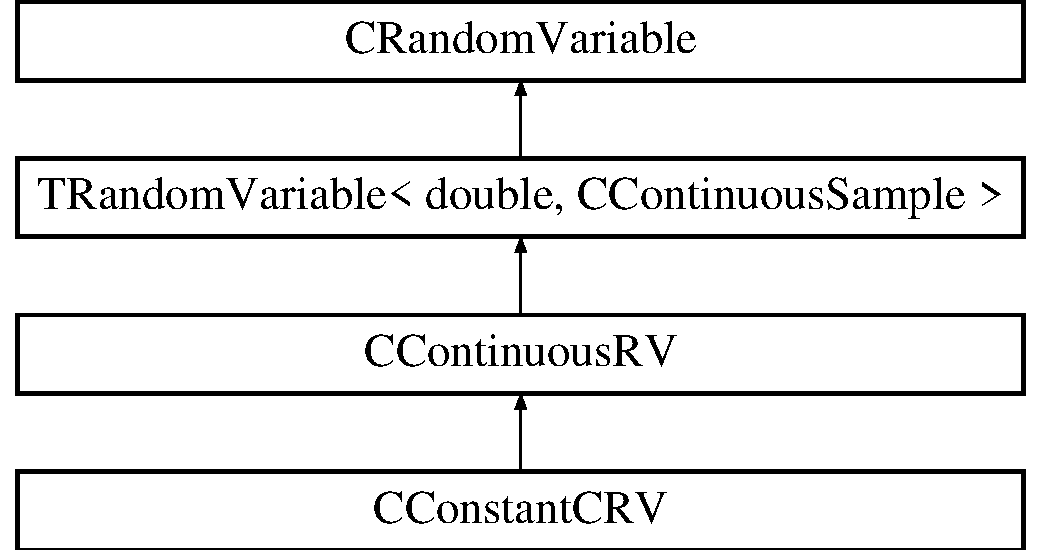
\includegraphics[height=4.000000cm]{class_c_constant_c_r_v}
\end{center}
\end{figure}
\subsection*{Public Member Functions}
\begin{DoxyCompactItemize}
\item 
\hyperlink{class_c_constant_c_r_v_a83c7a44fb68bf048527412009a612f61}{C\-Constant\-C\-R\-V} ()
\item 
virtual \hyperlink{class_c_constant_c_r_v_ab25575c114e0fe2165d8cb7ec12a65bb}{$\sim$\-C\-Constant\-C\-R\-V} ()
\item 
\hyperlink{class_c_constant_c_r_v_a3bf02e24577267e0bd1984358785d79c}{C\-Constant\-C\-R\-V} (const \hyperlink{class_c_constant_c_r_v}{C\-Constant\-C\-R\-V} \&O)
\item 
virtual void \hyperlink{class_c_constant_c_r_v_ac85e4654e4760830a461b128d1af0293}{set\-Distribution} (double \-\_\-xc, double \-\_\-dp2=0)
\begin{DoxyCompactList}\small\item\em Set distribution parameter. \end{DoxyCompactList}\item 
virtual void \hyperlink{class_c_constant_c_r_v_a96e78eee64773501b8c44001942a3d7d}{set\-Distribution} (const \hyperlink{class_c_continuous_sample}{C\-Continuous\-Sample} \&\-\_\-a\-S)
\begin{DoxyCompactList}\small\item\em Set distribution parameters from sample empirical parameters. \end{DoxyCompactList}\item 
virtual double \hyperlink{class_c_constant_c_r_v_a3b32fa2e4cad96f6e777126f4b970b10}{probability} (double \-\_\-x) const 
\begin{DoxyCompactList}\small\item\em Function that returns P\-M\-F. \end{DoxyCompactList}\item 
virtual double \hyperlink{class_c_constant_c_r_v_ad4cc2382b81238efe0f62eb97ce2f360}{cumulative} (double \-\_\-x) const 
\begin{DoxyCompactList}\small\item\em Function that returns C\-D\-F. \end{DoxyCompactList}\item 
virtual double \hyperlink{class_c_constant_c_r_v_ab6c57777abbff6cb66d95b96d3f089b8}{min\-Value} () const 
\begin{DoxyCompactList}\small\item\em Returns minimal value of the random variable. \end{DoxyCompactList}\item 
virtual double \hyperlink{class_c_constant_c_r_v_a33cd27bc45a581fdcb4f780387e90373}{max\-Value} () const 
\begin{DoxyCompactList}\small\item\em Returns maximal value of the random variable. \end{DoxyCompactList}\item 
virtual double \hyperlink{class_c_constant_c_r_v_a54ca9f831246b31679becf095aa655e3}{expected\-Value} () const 
\begin{DoxyCompactList}\small\item\em Returns expected value of the random variable. \end{DoxyCompactList}\item 
virtual \hyperlink{class_c_random_variable_a80d2a87c43847274138b51f7d713d7f1}{distributiontype} \hyperlink{class_c_constant_c_r_v_ab23347fb640e75308cf6dade83e0f9ae}{distribution\-Type} () const 
\begin{DoxyCompactList}\small\item\em Returns enum type of the random variable distribution. \end{DoxyCompactList}\item 
virtual std\-::string \hyperlink{class_c_constant_c_r_v_adf14a402f883d652657f53ab4a10d0be}{distribution\-Name} () const 
\begin{DoxyCompactList}\small\item\em Returns name of the random variable distribution. \end{DoxyCompactList}\item 
virtual Array\-Xd \hyperlink{class_c_constant_c_r_v_a19ccacd82627d70423d98f3cd81fb7b8}{export\-Domain} () const 
\begin{DoxyCompactList}\small\item\em Exports domain of the random variable. \end{DoxyCompactList}\item 
double \hyperlink{class_c_constant_c_r_v_a78b8c987ec4325a3e57c2c25effb851f}{constant\-Value} () const 
\begin{DoxyCompactList}\small\item\em Returns value of constant random variable. \end{DoxyCompactList}\item 
void \hyperlink{class_c_constant_c_r_v_a358c670636bdfdec515f279abd2db23a}{set\-Constant\-Value} (double \-\_\-xc)
\begin{DoxyCompactList}\small\item\em Sets value of constant random variable. \end{DoxyCompactList}\item 
virtual double \hyperlink{class_c_constant_c_r_v_a606fa01ade61968377b77fec8e22bb5b}{variance} () const 
\begin{DoxyCompactList}\small\item\em Returns variance of the random variable. \end{DoxyCompactList}\end{DoxyCompactItemize}
\subsection*{Protected Member Functions}
\begin{DoxyCompactItemize}
\item 
virtual double \hyperlink{class_c_constant_c_r_v_a7a3d90e12dbff50c473433f7d94de163}{do\-Quantile} (double \-\_\-p) const 
\begin{DoxyCompactList}\small\item\em Quantile, formula implementation. \end{DoxyCompactList}\end{DoxyCompactItemize}
\subsection*{Private Member Functions}
\begin{DoxyCompactItemize}
\item 
{\footnotesize template$<$class Archive $>$ }\\void \hyperlink{class_c_constant_c_r_v_a5fdc32e0b2c507f4c9e2532e57f93d59}{serialize} (Archive \&ar, const unsigned int version)
\end{DoxyCompactItemize}
\subsection*{Private Attributes}
\begin{DoxyCompactItemize}
\item 
double \hyperlink{class_c_constant_c_r_v_a2a82360ef61c3c3ea5b4728f82f3e489}{xc}
\end{DoxyCompactItemize}
\subsection*{Friends}
\begin{DoxyCompactItemize}
\item 
class \hyperlink{class_c_constant_c_r_v_ac98d07dd8f7b70e16ccb9a01abf56b9c}{boost\-::serialization\-::access}
\begin{DoxyCompactList}\small\item\em Boost serialization. \end{DoxyCompactList}\end{DoxyCompactItemize}
\subsection*{Additional Inherited Members}


\subsection{Detailed Description}
Class for constant continuous random variables derived from continuous random variables. 

\subsection{Constructor \& Destructor Documentation}
\hypertarget{class_c_constant_c_r_v_a83c7a44fb68bf048527412009a612f61}{\index{C\-Constant\-C\-R\-V@{C\-Constant\-C\-R\-V}!C\-Constant\-C\-R\-V@{C\-Constant\-C\-R\-V}}
\index{C\-Constant\-C\-R\-V@{C\-Constant\-C\-R\-V}!CConstantCRV@{C\-Constant\-C\-R\-V}}
\subsubsection[{C\-Constant\-C\-R\-V}]{\setlength{\rightskip}{0pt plus 5cm}C\-Constant\-C\-R\-V\-::\-C\-Constant\-C\-R\-V (
\begin{DoxyParamCaption}
{}
\end{DoxyParamCaption}
)\hspace{0.3cm}{\ttfamily [inline]}}}\label{class_c_constant_c_r_v_a83c7a44fb68bf048527412009a612f61}
\hypertarget{class_c_constant_c_r_v_ab25575c114e0fe2165d8cb7ec12a65bb}{\index{C\-Constant\-C\-R\-V@{C\-Constant\-C\-R\-V}!$\sim$\-C\-Constant\-C\-R\-V@{$\sim$\-C\-Constant\-C\-R\-V}}
\index{$\sim$\-C\-Constant\-C\-R\-V@{$\sim$\-C\-Constant\-C\-R\-V}!CConstantCRV@{C\-Constant\-C\-R\-V}}
\subsubsection[{$\sim$\-C\-Constant\-C\-R\-V}]{\setlength{\rightskip}{0pt plus 5cm}virtual C\-Constant\-C\-R\-V\-::$\sim$\-C\-Constant\-C\-R\-V (
\begin{DoxyParamCaption}
{}
\end{DoxyParamCaption}
)\hspace{0.3cm}{\ttfamily [inline]}, {\ttfamily [virtual]}}}\label{class_c_constant_c_r_v_ab25575c114e0fe2165d8cb7ec12a65bb}
\hypertarget{class_c_constant_c_r_v_a3bf02e24577267e0bd1984358785d79c}{\index{C\-Constant\-C\-R\-V@{C\-Constant\-C\-R\-V}!C\-Constant\-C\-R\-V@{C\-Constant\-C\-R\-V}}
\index{C\-Constant\-C\-R\-V@{C\-Constant\-C\-R\-V}!CConstantCRV@{C\-Constant\-C\-R\-V}}
\subsubsection[{C\-Constant\-C\-R\-V}]{\setlength{\rightskip}{0pt plus 5cm}C\-Constant\-C\-R\-V\-::\-C\-Constant\-C\-R\-V (
\begin{DoxyParamCaption}
\item[{const {\bf C\-Constant\-C\-R\-V} \&}]{O}
\end{DoxyParamCaption}
)\hspace{0.3cm}{\ttfamily [inline]}}}\label{class_c_constant_c_r_v_a3bf02e24577267e0bd1984358785d79c}


\subsection{Member Function Documentation}
\hypertarget{class_c_constant_c_r_v_a78b8c987ec4325a3e57c2c25effb851f}{\index{C\-Constant\-C\-R\-V@{C\-Constant\-C\-R\-V}!constant\-Value@{constant\-Value}}
\index{constant\-Value@{constant\-Value}!CConstantCRV@{C\-Constant\-C\-R\-V}}
\subsubsection[{constant\-Value}]{\setlength{\rightskip}{0pt plus 5cm}double C\-Constant\-C\-R\-V\-::constant\-Value (
\begin{DoxyParamCaption}
{}
\end{DoxyParamCaption}
) const\hspace{0.3cm}{\ttfamily [inline]}}}\label{class_c_constant_c_r_v_a78b8c987ec4325a3e57c2c25effb851f}


Returns value of constant random variable. 

\hypertarget{class_c_constant_c_r_v_ad4cc2382b81238efe0f62eb97ce2f360}{\index{C\-Constant\-C\-R\-V@{C\-Constant\-C\-R\-V}!cumulative@{cumulative}}
\index{cumulative@{cumulative}!CConstantCRV@{C\-Constant\-C\-R\-V}}
\subsubsection[{cumulative}]{\setlength{\rightskip}{0pt plus 5cm}virtual double C\-Constant\-C\-R\-V\-::cumulative (
\begin{DoxyParamCaption}
\item[{double}]{\-\_\-x}
\end{DoxyParamCaption}
) const\hspace{0.3cm}{\ttfamily [inline]}, {\ttfamily [virtual]}}}\label{class_c_constant_c_r_v_ad4cc2382b81238efe0f62eb97ce2f360}


Function that returns C\-D\-F. 

\hypertarget{class_c_constant_c_r_v_adf14a402f883d652657f53ab4a10d0be}{\index{C\-Constant\-C\-R\-V@{C\-Constant\-C\-R\-V}!distribution\-Name@{distribution\-Name}}
\index{distribution\-Name@{distribution\-Name}!CConstantCRV@{C\-Constant\-C\-R\-V}}
\subsubsection[{distribution\-Name}]{\setlength{\rightskip}{0pt plus 5cm}virtual std\-::string C\-Constant\-C\-R\-V\-::distribution\-Name (
\begin{DoxyParamCaption}
{}
\end{DoxyParamCaption}
) const\hspace{0.3cm}{\ttfamily [inline]}, {\ttfamily [virtual]}}}\label{class_c_constant_c_r_v_adf14a402f883d652657f53ab4a10d0be}


Returns name of the random variable distribution. 



Implements \hyperlink{class_c_random_variable_a4b33eef7c56f9f1a83af01fa8ef2502b}{C\-Random\-Variable}.

\hypertarget{class_c_constant_c_r_v_ab23347fb640e75308cf6dade83e0f9ae}{\index{C\-Constant\-C\-R\-V@{C\-Constant\-C\-R\-V}!distribution\-Type@{distribution\-Type}}
\index{distribution\-Type@{distribution\-Type}!CConstantCRV@{C\-Constant\-C\-R\-V}}
\subsubsection[{distribution\-Type}]{\setlength{\rightskip}{0pt plus 5cm}virtual {\bf distributiontype} C\-Constant\-C\-R\-V\-::distribution\-Type (
\begin{DoxyParamCaption}
{}
\end{DoxyParamCaption}
) const\hspace{0.3cm}{\ttfamily [inline]}, {\ttfamily [virtual]}}}\label{class_c_constant_c_r_v_ab23347fb640e75308cf6dade83e0f9ae}


Returns enum type of the random variable distribution. 



Implements \hyperlink{class_c_random_variable_a3b30589d41f4dd200bd40c8273cac2cd}{C\-Random\-Variable}.

\hypertarget{class_c_constant_c_r_v_a7a3d90e12dbff50c473433f7d94de163}{\index{C\-Constant\-C\-R\-V@{C\-Constant\-C\-R\-V}!do\-Quantile@{do\-Quantile}}
\index{do\-Quantile@{do\-Quantile}!CConstantCRV@{C\-Constant\-C\-R\-V}}
\subsubsection[{do\-Quantile}]{\setlength{\rightskip}{0pt plus 5cm}virtual double C\-Constant\-C\-R\-V\-::do\-Quantile (
\begin{DoxyParamCaption}
\item[{double}]{\-\_\-p}
\end{DoxyParamCaption}
) const\hspace{0.3cm}{\ttfamily [inline]}, {\ttfamily [protected]}, {\ttfamily [virtual]}}}\label{class_c_constant_c_r_v_a7a3d90e12dbff50c473433f7d94de163}


Quantile, formula implementation. 



Implements \hyperlink{class_c_random_variable_a552ab36c8144d7154cbe3cd363eee65b}{C\-Random\-Variable}.

\hypertarget{class_c_constant_c_r_v_a54ca9f831246b31679becf095aa655e3}{\index{C\-Constant\-C\-R\-V@{C\-Constant\-C\-R\-V}!expected\-Value@{expected\-Value}}
\index{expected\-Value@{expected\-Value}!CConstantCRV@{C\-Constant\-C\-R\-V}}
\subsubsection[{expected\-Value}]{\setlength{\rightskip}{0pt plus 5cm}virtual double C\-Constant\-C\-R\-V\-::expected\-Value (
\begin{DoxyParamCaption}
{}
\end{DoxyParamCaption}
) const\hspace{0.3cm}{\ttfamily [inline]}, {\ttfamily [virtual]}}}\label{class_c_constant_c_r_v_a54ca9f831246b31679becf095aa655e3}


Returns expected value of the random variable. 



Implements \hyperlink{class_c_random_variable_a6e5490d17f2b6abcf9922c8b1bd6d4ed}{C\-Random\-Variable}.

\hypertarget{class_c_constant_c_r_v_a19ccacd82627d70423d98f3cd81fb7b8}{\index{C\-Constant\-C\-R\-V@{C\-Constant\-C\-R\-V}!export\-Domain@{export\-Domain}}
\index{export\-Domain@{export\-Domain}!CConstantCRV@{C\-Constant\-C\-R\-V}}
\subsubsection[{export\-Domain}]{\setlength{\rightskip}{0pt plus 5cm}Array\-Xd C\-Constant\-C\-R\-V\-::export\-Domain (
\begin{DoxyParamCaption}
{}
\end{DoxyParamCaption}
) const\hspace{0.3cm}{\ttfamily [virtual]}}}\label{class_c_constant_c_r_v_a19ccacd82627d70423d98f3cd81fb7b8}


Exports domain of the random variable. 



Implements \hyperlink{class_t_random_variable_a37fc52d5fa37493a353887242d279a27}{T\-Random\-Variable$<$ t, T $>$}.

\hypertarget{class_c_constant_c_r_v_a33cd27bc45a581fdcb4f780387e90373}{\index{C\-Constant\-C\-R\-V@{C\-Constant\-C\-R\-V}!max\-Value@{max\-Value}}
\index{max\-Value@{max\-Value}!CConstantCRV@{C\-Constant\-C\-R\-V}}
\subsubsection[{max\-Value}]{\setlength{\rightskip}{0pt plus 5cm}virtual double C\-Constant\-C\-R\-V\-::max\-Value (
\begin{DoxyParamCaption}
{}
\end{DoxyParamCaption}
) const\hspace{0.3cm}{\ttfamily [inline]}, {\ttfamily [virtual]}}}\label{class_c_constant_c_r_v_a33cd27bc45a581fdcb4f780387e90373}


Returns maximal value of the random variable. 



Implements \hyperlink{class_c_random_variable_a48a5e98363d866f1f46568ed658479ad}{C\-Random\-Variable}.

\hypertarget{class_c_constant_c_r_v_ab6c57777abbff6cb66d95b96d3f089b8}{\index{C\-Constant\-C\-R\-V@{C\-Constant\-C\-R\-V}!min\-Value@{min\-Value}}
\index{min\-Value@{min\-Value}!CConstantCRV@{C\-Constant\-C\-R\-V}}
\subsubsection[{min\-Value}]{\setlength{\rightskip}{0pt plus 5cm}virtual double C\-Constant\-C\-R\-V\-::min\-Value (
\begin{DoxyParamCaption}
{}
\end{DoxyParamCaption}
) const\hspace{0.3cm}{\ttfamily [inline]}, {\ttfamily [virtual]}}}\label{class_c_constant_c_r_v_ab6c57777abbff6cb66d95b96d3f089b8}


Returns minimal value of the random variable. 



Implements \hyperlink{class_c_random_variable_a233ddd2eedb51b09a04a8c330646f356}{C\-Random\-Variable}.

\hypertarget{class_c_constant_c_r_v_a3b32fa2e4cad96f6e777126f4b970b10}{\index{C\-Constant\-C\-R\-V@{C\-Constant\-C\-R\-V}!probability@{probability}}
\index{probability@{probability}!CConstantCRV@{C\-Constant\-C\-R\-V}}
\subsubsection[{probability}]{\setlength{\rightskip}{0pt plus 5cm}virtual double C\-Constant\-C\-R\-V\-::probability (
\begin{DoxyParamCaption}
\item[{double}]{\-\_\-x}
\end{DoxyParamCaption}
) const\hspace{0.3cm}{\ttfamily [inline]}, {\ttfamily [virtual]}}}\label{class_c_constant_c_r_v_a3b32fa2e4cad96f6e777126f4b970b10}


Function that returns P\-M\-F. 

\hypertarget{class_c_constant_c_r_v_a5fdc32e0b2c507f4c9e2532e57f93d59}{\index{C\-Constant\-C\-R\-V@{C\-Constant\-C\-R\-V}!serialize@{serialize}}
\index{serialize@{serialize}!CConstantCRV@{C\-Constant\-C\-R\-V}}
\subsubsection[{serialize}]{\setlength{\rightskip}{0pt plus 5cm}template$<$class Archive $>$ void C\-Constant\-C\-R\-V\-::serialize (
\begin{DoxyParamCaption}
\item[{Archive \&}]{ar, }
\item[{const unsigned int}]{version}
\end{DoxyParamCaption}
)\hspace{0.3cm}{\ttfamily [private]}}}\label{class_c_constant_c_r_v_a5fdc32e0b2c507f4c9e2532e57f93d59}
\hypertarget{class_c_constant_c_r_v_a358c670636bdfdec515f279abd2db23a}{\index{C\-Constant\-C\-R\-V@{C\-Constant\-C\-R\-V}!set\-Constant\-Value@{set\-Constant\-Value}}
\index{set\-Constant\-Value@{set\-Constant\-Value}!CConstantCRV@{C\-Constant\-C\-R\-V}}
\subsubsection[{set\-Constant\-Value}]{\setlength{\rightskip}{0pt plus 5cm}void C\-Constant\-C\-R\-V\-::set\-Constant\-Value (
\begin{DoxyParamCaption}
\item[{double}]{\-\_\-xc}
\end{DoxyParamCaption}
)\hspace{0.3cm}{\ttfamily [inline]}}}\label{class_c_constant_c_r_v_a358c670636bdfdec515f279abd2db23a}


Sets value of constant random variable. 

\hypertarget{class_c_constant_c_r_v_ac85e4654e4760830a461b128d1af0293}{\index{C\-Constant\-C\-R\-V@{C\-Constant\-C\-R\-V}!set\-Distribution@{set\-Distribution}}
\index{set\-Distribution@{set\-Distribution}!CConstantCRV@{C\-Constant\-C\-R\-V}}
\subsubsection[{set\-Distribution}]{\setlength{\rightskip}{0pt plus 5cm}void C\-Constant\-C\-R\-V\-::set\-Distribution (
\begin{DoxyParamCaption}
\item[{double}]{\-\_\-xc, }
\item[{double}]{\-\_\-dp2 = {\ttfamily 0}}
\end{DoxyParamCaption}
)\hspace{0.3cm}{\ttfamily [virtual]}}}\label{class_c_constant_c_r_v_ac85e4654e4760830a461b128d1af0293}


Set distribution parameter. 

\hypertarget{class_c_constant_c_r_v_a96e78eee64773501b8c44001942a3d7d}{\index{C\-Constant\-C\-R\-V@{C\-Constant\-C\-R\-V}!set\-Distribution@{set\-Distribution}}
\index{set\-Distribution@{set\-Distribution}!CConstantCRV@{C\-Constant\-C\-R\-V}}
\subsubsection[{set\-Distribution}]{\setlength{\rightskip}{0pt plus 5cm}virtual void C\-Constant\-C\-R\-V\-::set\-Distribution (
\begin{DoxyParamCaption}
\item[{const {\bf C\-Continuous\-Sample} \&}]{\-\_\-a\-S}
\end{DoxyParamCaption}
)\hspace{0.3cm}{\ttfamily [inline]}, {\ttfamily [virtual]}}}\label{class_c_constant_c_r_v_a96e78eee64773501b8c44001942a3d7d}


Set distribution parameters from sample empirical parameters. 

\hypertarget{class_c_constant_c_r_v_a606fa01ade61968377b77fec8e22bb5b}{\index{C\-Constant\-C\-R\-V@{C\-Constant\-C\-R\-V}!variance@{variance}}
\index{variance@{variance}!CConstantCRV@{C\-Constant\-C\-R\-V}}
\subsubsection[{variance}]{\setlength{\rightskip}{0pt plus 5cm}virtual double C\-Constant\-C\-R\-V\-::variance (
\begin{DoxyParamCaption}
{}
\end{DoxyParamCaption}
) const\hspace{0.3cm}{\ttfamily [inline]}, {\ttfamily [virtual]}}}\label{class_c_constant_c_r_v_a606fa01ade61968377b77fec8e22bb5b}


Returns variance of the random variable. 



Implements \hyperlink{class_c_random_variable_a3b0b87c4aab74c0406cd8321b8b96747}{C\-Random\-Variable}.



\subsection{Friends And Related Function Documentation}
\hypertarget{class_c_constant_c_r_v_ac98d07dd8f7b70e16ccb9a01abf56b9c}{\index{C\-Constant\-C\-R\-V@{C\-Constant\-C\-R\-V}!boost\-::serialization\-::access@{boost\-::serialization\-::access}}
\index{boost\-::serialization\-::access@{boost\-::serialization\-::access}!CConstantCRV@{C\-Constant\-C\-R\-V}}
\subsubsection[{boost\-::serialization\-::access}]{\setlength{\rightskip}{0pt plus 5cm}friend class boost\-::serialization\-::access\hspace{0.3cm}{\ttfamily [friend]}}}\label{class_c_constant_c_r_v_ac98d07dd8f7b70e16ccb9a01abf56b9c}


Boost serialization. 



\subsection{Member Data Documentation}
\hypertarget{class_c_constant_c_r_v_a2a82360ef61c3c3ea5b4728f82f3e489}{\index{C\-Constant\-C\-R\-V@{C\-Constant\-C\-R\-V}!xc@{xc}}
\index{xc@{xc}!CConstantCRV@{C\-Constant\-C\-R\-V}}
\subsubsection[{xc}]{\setlength{\rightskip}{0pt plus 5cm}double C\-Constant\-C\-R\-V\-::xc\hspace{0.3cm}{\ttfamily [private]}}}\label{class_c_constant_c_r_v_a2a82360ef61c3c3ea5b4728f82f3e489}
Distribution parameter\-: constant integer value of the random varialbe. 

The documentation for this class was generated from the following files\-:\begin{DoxyCompactItemize}
\item 
C\-:/\-Development/core/\hyperlink{_random_variable_8h}{Random\-Variable.\-h}\item 
C\-:/\-Development/core/\hyperlink{_random_variable_8cpp}{Random\-Variable.\-cpp}\end{DoxyCompactItemize}

\hypertarget{class_c_constant_d_r_v}{\section{C\-Constant\-D\-R\-V Class Reference}
\label{class_c_constant_d_r_v}\index{C\-Constant\-D\-R\-V@{C\-Constant\-D\-R\-V}}
}


Class for constant discrete random variables derived from discrete random variables.  




{\ttfamily \#include $<$Random\-Variable.\-h$>$}

Inheritance diagram for C\-Constant\-D\-R\-V\-:\begin{figure}[H]
\begin{center}
\leavevmode
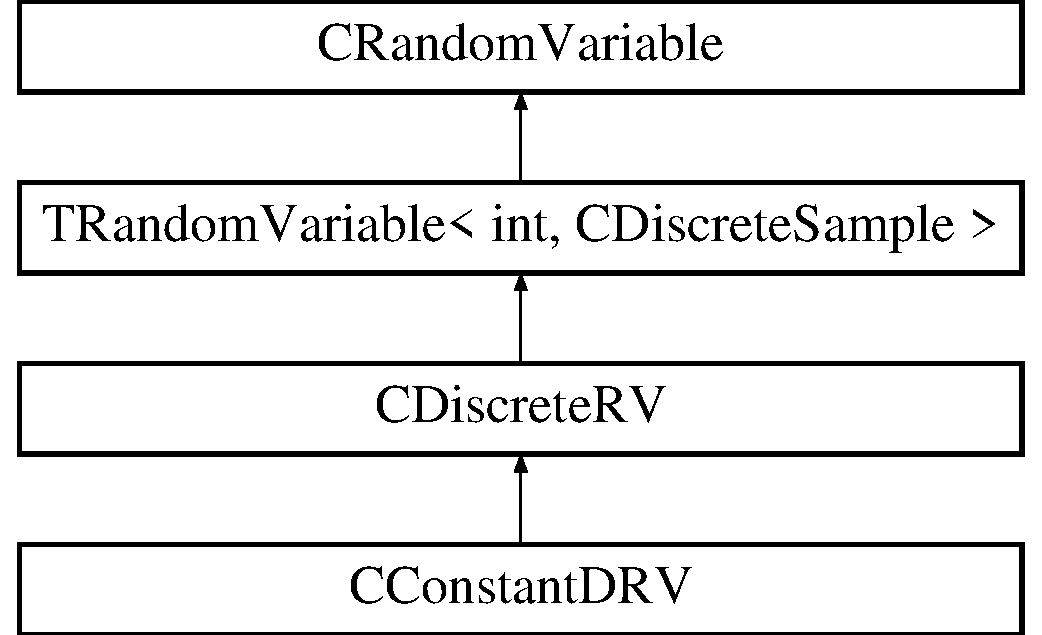
\includegraphics[height=4.000000cm]{class_c_constant_d_r_v}
\end{center}
\end{figure}
\subsection*{Public Member Functions}
\begin{DoxyCompactItemize}
\item 
\hyperlink{class_c_constant_d_r_v_a0c3499451fe54b1a42c6a26474c344aa}{C\-Constant\-D\-R\-V} ()
\item 
virtual \hyperlink{class_c_constant_d_r_v_a1f600cdc9a090e01266c29b19896e5af}{$\sim$\-C\-Constant\-D\-R\-V} ()
\item 
\hyperlink{class_c_constant_d_r_v_a9404234b2ec170d0b8195c11b7bd48ab}{C\-Constant\-D\-R\-V} (const \hyperlink{class_c_constant_d_r_v}{C\-Constant\-D\-R\-V} \&O)
\item 
virtual void \hyperlink{class_c_constant_d_r_v_a524e6add6b635ea92fe7d67ef3c56043}{set\-Distribution} (int \-\_\-c, int \-\_\-dp2=0)
\begin{DoxyCompactList}\small\item\em Set distribution parameter. \end{DoxyCompactList}\item 
virtual void \hyperlink{class_c_constant_d_r_v_a2f5dec9082ba7b2c6174df6c1d04917e}{set\-Distribution} (const \hyperlink{class_c_discrete_sample}{C\-Discrete\-Sample} \&\-\_\-a\-S)
\begin{DoxyCompactList}\small\item\em Computes P\-M\-F and C\-D\-F from sample histogram. \end{DoxyCompactList}\item 
virtual double \hyperlink{class_c_constant_d_r_v_a15e7dab1acdb0e1fb7eb6031e5ca1beb}{probability} (int \-\_\-k) const 
\begin{DoxyCompactList}\small\item\em Function that returns P\-M\-F. \end{DoxyCompactList}\item 
virtual double \hyperlink{class_c_constant_d_r_v_a3ff0806ce1d6875bcce0382222a7b564}{cumulative} (int \-\_\-k) const 
\begin{DoxyCompactList}\small\item\em Function that returns C\-D\-F. \end{DoxyCompactList}\item 
virtual double \hyperlink{class_c_constant_d_r_v_a85930e45d6e50977773fd963f88f2f44}{min\-Value} () const 
\begin{DoxyCompactList}\small\item\em Returns minimal value of the random variable. \end{DoxyCompactList}\item 
virtual double \hyperlink{class_c_constant_d_r_v_a602bcf72b61be44f61c00eab0569b17e}{max\-Value} () const 
\begin{DoxyCompactList}\small\item\em Returns maximal value of the random variable. \end{DoxyCompactList}\item 
virtual double \hyperlink{class_c_constant_d_r_v_a975c37d9fd5106627cec49dcf6eea9b7}{expected\-Value} () const 
\begin{DoxyCompactList}\small\item\em Returns expected value of the random variable. \end{DoxyCompactList}\item 
virtual \hyperlink{class_c_random_variable_a80d2a87c43847274138b51f7d713d7f1}{distributiontype} \hyperlink{class_c_constant_d_r_v_a0bdcae8cb3bcbf77480aabf0ce8773e7}{distribution\-Type} () const 
\begin{DoxyCompactList}\small\item\em Returns enum type of the random variable distribution. \end{DoxyCompactList}\item 
virtual std\-::string \hyperlink{class_c_constant_d_r_v_abdd844ca2211966c00f0f9205778feec}{distribution\-Name} () const 
\begin{DoxyCompactList}\small\item\em Returns name of the random variable distribution. \end{DoxyCompactList}\item 
virtual Array\-Xi \hyperlink{class_c_constant_d_r_v_a66b319e508f2a174bf572884183aeee8}{export\-Domain} () const 
\begin{DoxyCompactList}\small\item\em Exports domain of the random variable. \end{DoxyCompactList}\item 
int \hyperlink{class_c_constant_d_r_v_a77a2209435ebee42a571f5890c3440dc}{constant\-Value} () const 
\begin{DoxyCompactList}\small\item\em Returns value of constant random variable. \end{DoxyCompactList}\item 
void \hyperlink{class_c_constant_d_r_v_afe331bab81ade39b1c26b8e6057e55a9}{set\-Constant\-Value} (int \-\_\-c)
\begin{DoxyCompactList}\small\item\em Sets value of constant random variable. \end{DoxyCompactList}\item 
virtual double \hyperlink{class_c_constant_d_r_v_a17369981ab38b3cb839cc16d596a12a6}{variance} () const 
\begin{DoxyCompactList}\small\item\em Returns variance of the random variable. \end{DoxyCompactList}\end{DoxyCompactItemize}
\subsection*{Protected Member Functions}
\begin{DoxyCompactItemize}
\item 
virtual double \hyperlink{class_c_constant_d_r_v_a8ddf0c49c7b4e0a5b593add04721568e}{do\-Quantile} (double \-\_\-p) const 
\begin{DoxyCompactList}\small\item\em Quantile, formula implementation. \end{DoxyCompactList}\end{DoxyCompactItemize}
\subsection*{Private Member Functions}
\begin{DoxyCompactItemize}
\item 
{\footnotesize template$<$class Archive $>$ }\\void \hyperlink{class_c_constant_d_r_v_abe6f147ae70c0e9087e4e2a1fc2f105a}{serialize} (Archive \&ar, const unsigned int version)
\end{DoxyCompactItemize}
\subsection*{Private Attributes}
\begin{DoxyCompactItemize}
\item 
int \hyperlink{class_c_constant_d_r_v_a5cabcca79ea5f4c87e8f6c9b0a4e1412}{c}
\end{DoxyCompactItemize}
\subsection*{Friends}
\begin{DoxyCompactItemize}
\item 
class \hyperlink{class_c_constant_d_r_v_ac98d07dd8f7b70e16ccb9a01abf56b9c}{boost\-::serialization\-::access}
\begin{DoxyCompactList}\small\item\em Boost serialization. \end{DoxyCompactList}\end{DoxyCompactItemize}
\subsection*{Additional Inherited Members}


\subsection{Detailed Description}
Class for constant discrete random variables derived from discrete random variables. 

\subsection{Constructor \& Destructor Documentation}
\hypertarget{class_c_constant_d_r_v_a0c3499451fe54b1a42c6a26474c344aa}{\index{C\-Constant\-D\-R\-V@{C\-Constant\-D\-R\-V}!C\-Constant\-D\-R\-V@{C\-Constant\-D\-R\-V}}
\index{C\-Constant\-D\-R\-V@{C\-Constant\-D\-R\-V}!CConstantDRV@{C\-Constant\-D\-R\-V}}
\subsubsection[{C\-Constant\-D\-R\-V}]{\setlength{\rightskip}{0pt plus 5cm}C\-Constant\-D\-R\-V\-::\-C\-Constant\-D\-R\-V (
\begin{DoxyParamCaption}
{}
\end{DoxyParamCaption}
)\hspace{0.3cm}{\ttfamily [inline]}}}\label{class_c_constant_d_r_v_a0c3499451fe54b1a42c6a26474c344aa}
\hypertarget{class_c_constant_d_r_v_a1f600cdc9a090e01266c29b19896e5af}{\index{C\-Constant\-D\-R\-V@{C\-Constant\-D\-R\-V}!$\sim$\-C\-Constant\-D\-R\-V@{$\sim$\-C\-Constant\-D\-R\-V}}
\index{$\sim$\-C\-Constant\-D\-R\-V@{$\sim$\-C\-Constant\-D\-R\-V}!CConstantDRV@{C\-Constant\-D\-R\-V}}
\subsubsection[{$\sim$\-C\-Constant\-D\-R\-V}]{\setlength{\rightskip}{0pt plus 5cm}virtual C\-Constant\-D\-R\-V\-::$\sim$\-C\-Constant\-D\-R\-V (
\begin{DoxyParamCaption}
{}
\end{DoxyParamCaption}
)\hspace{0.3cm}{\ttfamily [inline]}, {\ttfamily [virtual]}}}\label{class_c_constant_d_r_v_a1f600cdc9a090e01266c29b19896e5af}
\hypertarget{class_c_constant_d_r_v_a9404234b2ec170d0b8195c11b7bd48ab}{\index{C\-Constant\-D\-R\-V@{C\-Constant\-D\-R\-V}!C\-Constant\-D\-R\-V@{C\-Constant\-D\-R\-V}}
\index{C\-Constant\-D\-R\-V@{C\-Constant\-D\-R\-V}!CConstantDRV@{C\-Constant\-D\-R\-V}}
\subsubsection[{C\-Constant\-D\-R\-V}]{\setlength{\rightskip}{0pt plus 5cm}C\-Constant\-D\-R\-V\-::\-C\-Constant\-D\-R\-V (
\begin{DoxyParamCaption}
\item[{const {\bf C\-Constant\-D\-R\-V} \&}]{O}
\end{DoxyParamCaption}
)\hspace{0.3cm}{\ttfamily [inline]}}}\label{class_c_constant_d_r_v_a9404234b2ec170d0b8195c11b7bd48ab}


\subsection{Member Function Documentation}
\hypertarget{class_c_constant_d_r_v_a77a2209435ebee42a571f5890c3440dc}{\index{C\-Constant\-D\-R\-V@{C\-Constant\-D\-R\-V}!constant\-Value@{constant\-Value}}
\index{constant\-Value@{constant\-Value}!CConstantDRV@{C\-Constant\-D\-R\-V}}
\subsubsection[{constant\-Value}]{\setlength{\rightskip}{0pt plus 5cm}int C\-Constant\-D\-R\-V\-::constant\-Value (
\begin{DoxyParamCaption}
{}
\end{DoxyParamCaption}
) const\hspace{0.3cm}{\ttfamily [inline]}}}\label{class_c_constant_d_r_v_a77a2209435ebee42a571f5890c3440dc}


Returns value of constant random variable. 

\hypertarget{class_c_constant_d_r_v_a3ff0806ce1d6875bcce0382222a7b564}{\index{C\-Constant\-D\-R\-V@{C\-Constant\-D\-R\-V}!cumulative@{cumulative}}
\index{cumulative@{cumulative}!CConstantDRV@{C\-Constant\-D\-R\-V}}
\subsubsection[{cumulative}]{\setlength{\rightskip}{0pt plus 5cm}virtual double C\-Constant\-D\-R\-V\-::cumulative (
\begin{DoxyParamCaption}
\item[{int}]{\-\_\-k}
\end{DoxyParamCaption}
) const\hspace{0.3cm}{\ttfamily [inline]}, {\ttfamily [virtual]}}}\label{class_c_constant_d_r_v_a3ff0806ce1d6875bcce0382222a7b564}


Function that returns C\-D\-F. 

\hypertarget{class_c_constant_d_r_v_abdd844ca2211966c00f0f9205778feec}{\index{C\-Constant\-D\-R\-V@{C\-Constant\-D\-R\-V}!distribution\-Name@{distribution\-Name}}
\index{distribution\-Name@{distribution\-Name}!CConstantDRV@{C\-Constant\-D\-R\-V}}
\subsubsection[{distribution\-Name}]{\setlength{\rightskip}{0pt plus 5cm}virtual std\-::string C\-Constant\-D\-R\-V\-::distribution\-Name (
\begin{DoxyParamCaption}
{}
\end{DoxyParamCaption}
) const\hspace{0.3cm}{\ttfamily [inline]}, {\ttfamily [virtual]}}}\label{class_c_constant_d_r_v_abdd844ca2211966c00f0f9205778feec}


Returns name of the random variable distribution. 



Implements \hyperlink{class_c_random_variable_a4b33eef7c56f9f1a83af01fa8ef2502b}{C\-Random\-Variable}.

\hypertarget{class_c_constant_d_r_v_a0bdcae8cb3bcbf77480aabf0ce8773e7}{\index{C\-Constant\-D\-R\-V@{C\-Constant\-D\-R\-V}!distribution\-Type@{distribution\-Type}}
\index{distribution\-Type@{distribution\-Type}!CConstantDRV@{C\-Constant\-D\-R\-V}}
\subsubsection[{distribution\-Type}]{\setlength{\rightskip}{0pt plus 5cm}virtual {\bf distributiontype} C\-Constant\-D\-R\-V\-::distribution\-Type (
\begin{DoxyParamCaption}
{}
\end{DoxyParamCaption}
) const\hspace{0.3cm}{\ttfamily [inline]}, {\ttfamily [virtual]}}}\label{class_c_constant_d_r_v_a0bdcae8cb3bcbf77480aabf0ce8773e7}


Returns enum type of the random variable distribution. 



Implements \hyperlink{class_c_random_variable_a3b30589d41f4dd200bd40c8273cac2cd}{C\-Random\-Variable}.

\hypertarget{class_c_constant_d_r_v_a8ddf0c49c7b4e0a5b593add04721568e}{\index{C\-Constant\-D\-R\-V@{C\-Constant\-D\-R\-V}!do\-Quantile@{do\-Quantile}}
\index{do\-Quantile@{do\-Quantile}!CConstantDRV@{C\-Constant\-D\-R\-V}}
\subsubsection[{do\-Quantile}]{\setlength{\rightskip}{0pt plus 5cm}virtual double C\-Constant\-D\-R\-V\-::do\-Quantile (
\begin{DoxyParamCaption}
\item[{double}]{\-\_\-p}
\end{DoxyParamCaption}
) const\hspace{0.3cm}{\ttfamily [inline]}, {\ttfamily [protected]}, {\ttfamily [virtual]}}}\label{class_c_constant_d_r_v_a8ddf0c49c7b4e0a5b593add04721568e}


Quantile, formula implementation. 



Implements \hyperlink{class_c_random_variable_a552ab36c8144d7154cbe3cd363eee65b}{C\-Random\-Variable}.

\hypertarget{class_c_constant_d_r_v_a975c37d9fd5106627cec49dcf6eea9b7}{\index{C\-Constant\-D\-R\-V@{C\-Constant\-D\-R\-V}!expected\-Value@{expected\-Value}}
\index{expected\-Value@{expected\-Value}!CConstantDRV@{C\-Constant\-D\-R\-V}}
\subsubsection[{expected\-Value}]{\setlength{\rightskip}{0pt plus 5cm}virtual double C\-Constant\-D\-R\-V\-::expected\-Value (
\begin{DoxyParamCaption}
{}
\end{DoxyParamCaption}
) const\hspace{0.3cm}{\ttfamily [inline]}, {\ttfamily [virtual]}}}\label{class_c_constant_d_r_v_a975c37d9fd5106627cec49dcf6eea9b7}


Returns expected value of the random variable. 



Implements \hyperlink{class_c_random_variable_a6e5490d17f2b6abcf9922c8b1bd6d4ed}{C\-Random\-Variable}.

\hypertarget{class_c_constant_d_r_v_a66b319e508f2a174bf572884183aeee8}{\index{C\-Constant\-D\-R\-V@{C\-Constant\-D\-R\-V}!export\-Domain@{export\-Domain}}
\index{export\-Domain@{export\-Domain}!CConstantDRV@{C\-Constant\-D\-R\-V}}
\subsubsection[{export\-Domain}]{\setlength{\rightskip}{0pt plus 5cm}Array\-Xi C\-Constant\-D\-R\-V\-::export\-Domain (
\begin{DoxyParamCaption}
{}
\end{DoxyParamCaption}
) const\hspace{0.3cm}{\ttfamily [virtual]}}}\label{class_c_constant_d_r_v_a66b319e508f2a174bf572884183aeee8}


Exports domain of the random variable. 



Implements \hyperlink{class_t_random_variable_a37fc52d5fa37493a353887242d279a27}{T\-Random\-Variable$<$ t, T $>$}.

\hypertarget{class_c_constant_d_r_v_a602bcf72b61be44f61c00eab0569b17e}{\index{C\-Constant\-D\-R\-V@{C\-Constant\-D\-R\-V}!max\-Value@{max\-Value}}
\index{max\-Value@{max\-Value}!CConstantDRV@{C\-Constant\-D\-R\-V}}
\subsubsection[{max\-Value}]{\setlength{\rightskip}{0pt plus 5cm}virtual double C\-Constant\-D\-R\-V\-::max\-Value (
\begin{DoxyParamCaption}
{}
\end{DoxyParamCaption}
) const\hspace{0.3cm}{\ttfamily [inline]}, {\ttfamily [virtual]}}}\label{class_c_constant_d_r_v_a602bcf72b61be44f61c00eab0569b17e}


Returns maximal value of the random variable. 



Implements \hyperlink{class_c_random_variable_a48a5e98363d866f1f46568ed658479ad}{C\-Random\-Variable}.

\hypertarget{class_c_constant_d_r_v_a85930e45d6e50977773fd963f88f2f44}{\index{C\-Constant\-D\-R\-V@{C\-Constant\-D\-R\-V}!min\-Value@{min\-Value}}
\index{min\-Value@{min\-Value}!CConstantDRV@{C\-Constant\-D\-R\-V}}
\subsubsection[{min\-Value}]{\setlength{\rightskip}{0pt plus 5cm}virtual double C\-Constant\-D\-R\-V\-::min\-Value (
\begin{DoxyParamCaption}
{}
\end{DoxyParamCaption}
) const\hspace{0.3cm}{\ttfamily [inline]}, {\ttfamily [virtual]}}}\label{class_c_constant_d_r_v_a85930e45d6e50977773fd963f88f2f44}


Returns minimal value of the random variable. 



Implements \hyperlink{class_c_random_variable_a233ddd2eedb51b09a04a8c330646f356}{C\-Random\-Variable}.

\hypertarget{class_c_constant_d_r_v_a15e7dab1acdb0e1fb7eb6031e5ca1beb}{\index{C\-Constant\-D\-R\-V@{C\-Constant\-D\-R\-V}!probability@{probability}}
\index{probability@{probability}!CConstantDRV@{C\-Constant\-D\-R\-V}}
\subsubsection[{probability}]{\setlength{\rightskip}{0pt plus 5cm}virtual double C\-Constant\-D\-R\-V\-::probability (
\begin{DoxyParamCaption}
\item[{int}]{\-\_\-k}
\end{DoxyParamCaption}
) const\hspace{0.3cm}{\ttfamily [inline]}, {\ttfamily [virtual]}}}\label{class_c_constant_d_r_v_a15e7dab1acdb0e1fb7eb6031e5ca1beb}


Function that returns P\-M\-F. 

\hypertarget{class_c_constant_d_r_v_abe6f147ae70c0e9087e4e2a1fc2f105a}{\index{C\-Constant\-D\-R\-V@{C\-Constant\-D\-R\-V}!serialize@{serialize}}
\index{serialize@{serialize}!CConstantDRV@{C\-Constant\-D\-R\-V}}
\subsubsection[{serialize}]{\setlength{\rightskip}{0pt plus 5cm}template$<$class Archive $>$ void C\-Constant\-D\-R\-V\-::serialize (
\begin{DoxyParamCaption}
\item[{Archive \&}]{ar, }
\item[{const unsigned int}]{version}
\end{DoxyParamCaption}
)\hspace{0.3cm}{\ttfamily [private]}}}\label{class_c_constant_d_r_v_abe6f147ae70c0e9087e4e2a1fc2f105a}
\hypertarget{class_c_constant_d_r_v_afe331bab81ade39b1c26b8e6057e55a9}{\index{C\-Constant\-D\-R\-V@{C\-Constant\-D\-R\-V}!set\-Constant\-Value@{set\-Constant\-Value}}
\index{set\-Constant\-Value@{set\-Constant\-Value}!CConstantDRV@{C\-Constant\-D\-R\-V}}
\subsubsection[{set\-Constant\-Value}]{\setlength{\rightskip}{0pt plus 5cm}void C\-Constant\-D\-R\-V\-::set\-Constant\-Value (
\begin{DoxyParamCaption}
\item[{int}]{\-\_\-c}
\end{DoxyParamCaption}
)\hspace{0.3cm}{\ttfamily [inline]}}}\label{class_c_constant_d_r_v_afe331bab81ade39b1c26b8e6057e55a9}


Sets value of constant random variable. 

\hypertarget{class_c_constant_d_r_v_a524e6add6b635ea92fe7d67ef3c56043}{\index{C\-Constant\-D\-R\-V@{C\-Constant\-D\-R\-V}!set\-Distribution@{set\-Distribution}}
\index{set\-Distribution@{set\-Distribution}!CConstantDRV@{C\-Constant\-D\-R\-V}}
\subsubsection[{set\-Distribution}]{\setlength{\rightskip}{0pt plus 5cm}void C\-Constant\-D\-R\-V\-::set\-Distribution (
\begin{DoxyParamCaption}
\item[{int}]{\-\_\-c, }
\item[{int}]{\-\_\-dp2 = {\ttfamily 0}}
\end{DoxyParamCaption}
)\hspace{0.3cm}{\ttfamily [virtual]}}}\label{class_c_constant_d_r_v_a524e6add6b635ea92fe7d67ef3c56043}


Set distribution parameter. 

\hypertarget{class_c_constant_d_r_v_a2f5dec9082ba7b2c6174df6c1d04917e}{\index{C\-Constant\-D\-R\-V@{C\-Constant\-D\-R\-V}!set\-Distribution@{set\-Distribution}}
\index{set\-Distribution@{set\-Distribution}!CConstantDRV@{C\-Constant\-D\-R\-V}}
\subsubsection[{set\-Distribution}]{\setlength{\rightskip}{0pt plus 5cm}virtual void C\-Constant\-D\-R\-V\-::set\-Distribution (
\begin{DoxyParamCaption}
\item[{const {\bf C\-Discrete\-Sample} \&}]{\-\_\-a\-S}
\end{DoxyParamCaption}
)\hspace{0.3cm}{\ttfamily [inline]}, {\ttfamily [virtual]}}}\label{class_c_constant_d_r_v_a2f5dec9082ba7b2c6174df6c1d04917e}


Computes P\-M\-F and C\-D\-F from sample histogram. 

\hypertarget{class_c_constant_d_r_v_a17369981ab38b3cb839cc16d596a12a6}{\index{C\-Constant\-D\-R\-V@{C\-Constant\-D\-R\-V}!variance@{variance}}
\index{variance@{variance}!CConstantDRV@{C\-Constant\-D\-R\-V}}
\subsubsection[{variance}]{\setlength{\rightskip}{0pt plus 5cm}virtual double C\-Constant\-D\-R\-V\-::variance (
\begin{DoxyParamCaption}
{}
\end{DoxyParamCaption}
) const\hspace{0.3cm}{\ttfamily [inline]}, {\ttfamily [virtual]}}}\label{class_c_constant_d_r_v_a17369981ab38b3cb839cc16d596a12a6}


Returns variance of the random variable. 



Implements \hyperlink{class_c_random_variable_a3b0b87c4aab74c0406cd8321b8b96747}{C\-Random\-Variable}.



\subsection{Friends And Related Function Documentation}
\hypertarget{class_c_constant_d_r_v_ac98d07dd8f7b70e16ccb9a01abf56b9c}{\index{C\-Constant\-D\-R\-V@{C\-Constant\-D\-R\-V}!boost\-::serialization\-::access@{boost\-::serialization\-::access}}
\index{boost\-::serialization\-::access@{boost\-::serialization\-::access}!CConstantDRV@{C\-Constant\-D\-R\-V}}
\subsubsection[{boost\-::serialization\-::access}]{\setlength{\rightskip}{0pt plus 5cm}friend class boost\-::serialization\-::access\hspace{0.3cm}{\ttfamily [friend]}}}\label{class_c_constant_d_r_v_ac98d07dd8f7b70e16ccb9a01abf56b9c}


Boost serialization. 



\subsection{Member Data Documentation}
\hypertarget{class_c_constant_d_r_v_a5cabcca79ea5f4c87e8f6c9b0a4e1412}{\index{C\-Constant\-D\-R\-V@{C\-Constant\-D\-R\-V}!c@{c}}
\index{c@{c}!CConstantDRV@{C\-Constant\-D\-R\-V}}
\subsubsection[{c}]{\setlength{\rightskip}{0pt plus 5cm}int C\-Constant\-D\-R\-V\-::c\hspace{0.3cm}{\ttfamily [private]}}}\label{class_c_constant_d_r_v_a5cabcca79ea5f4c87e8f6c9b0a4e1412}
Distribution parameter\-: constant integer value of the random variable. 

The documentation for this class was generated from the following files\-:\begin{DoxyCompactItemize}
\item 
C\-:/\-Development/core/\hyperlink{_random_variable_8h}{Random\-Variable.\-h}\item 
C\-:/\-Development/core/\hyperlink{_random_variable_8cpp}{Random\-Variable.\-cpp}\end{DoxyCompactItemize}

\hypertarget{class_go_s_u_m_1_1_c_constraints}{\section{Go\-S\-U\-M\-:\-:C\-Constraints Class Reference}
\label{class_go_s_u_m_1_1_c_constraints}\index{Go\-S\-U\-M\-::\-C\-Constraints@{Go\-S\-U\-M\-::\-C\-Constraints}}
}


Class for the constraints with parser functions.  




{\ttfamily \#include $<$Constraints.\-h$>$}

Inheritance diagram for Go\-S\-U\-M\-:\-:C\-Constraints\-:\begin{figure}[H]
\begin{center}
\leavevmode
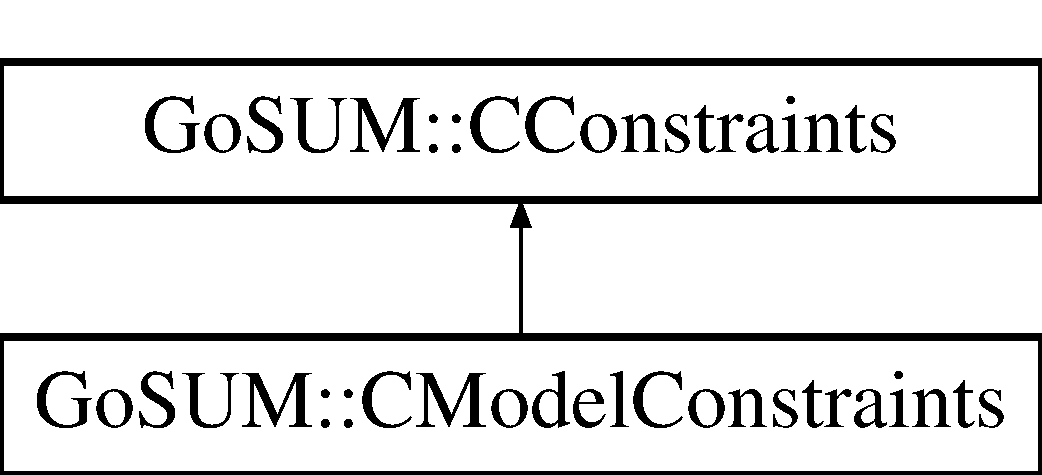
\includegraphics[height=2.000000cm]{class_go_s_u_m_1_1_c_constraints}
\end{center}
\end{figure}
\subsection*{Public Member Functions}
\begin{DoxyCompactItemize}
\item 
\hyperlink{class_go_s_u_m_1_1_c_constraints_ad4a1d290fbe6e1932b08f4fb1695b0a6}{C\-Constraints} ()
\item 
virtual \hyperlink{class_go_s_u_m_1_1_c_constraints_a79a84d644f7e8022ce16487b4707bc33}{$\sim$\-C\-Constraints} ()
\item 
virtual void \hyperlink{class_go_s_u_m_1_1_c_constraints_a45acde7b103ba957a718031b6ecebf69}{clear} ()
\begin{DoxyCompactList}\small\item\em Clears object. \end{DoxyCompactList}\item 
int \hyperlink{class_go_s_u_m_1_1_c_constraints_a9979ee367d1f0592e0ddea874307527c}{size} () const 
\begin{DoxyCompactList}\small\item\em Returns size of the constraints. \end{DoxyCompactList}\item 
void \hyperlink{class_go_s_u_m_1_1_c_constraints_ab50ae4d923f0a67ed6bf468b2e7b3b8b}{add\-Expression} (const std\-::string \&\-\_\-gexpr)
\begin{DoxyCompactList}\small\item\em Adds contraint expression. \end{DoxyCompactList}\item 
void \hyperlink{class_go_s_u_m_1_1_c_constraints_a8c242c266df5f843807e3f000e724929}{erase\-Expression} (int \-\_\-at)
\begin{DoxyCompactList}\small\item\em Erases particular constraint expression. \end{DoxyCompactList}\item 
void \hyperlink{class_go_s_u_m_1_1_c_constraints_a75b0405e1cb0c978c5eccc5df2fdbd8a}{set\-Expression} (const std\-::string \&\-\_\-gexpr, int \-\_\-at)
\begin{DoxyCompactList}\small\item\em Sets particular cosntraint expression. \end{DoxyCompactList}\item 
std\-::string \hyperlink{class_go_s_u_m_1_1_c_constraints_af1e75f5d326a3466c2c778ccca1d82fe}{expression} (int \-\_\-at) const 
\begin{DoxyCompactList}\small\item\em Returns particular constraint expression. \end{DoxyCompactList}\item 
std\-::string \hyperlink{class_go_s_u_m_1_1_c_constraints_ae1263ac8c72174dddef6496492c9d7ad}{roundoff\-Equality} (std\-::string \-\_\-expr)
\begin{DoxyCompactList}\small\item\em If \-\_\-expr is an equality expression left=right it returns expression abs(left-\/right)$<$=T\-I\-N\-Y. \end{DoxyCompactList}\item 
bool \hyperlink{class_go_s_u_m_1_1_c_constraints_ab27d71bea1ae044f44b172100b9dfbe7}{validate\-Expressions} ()
\begin{DoxyCompactList}\small\item\em Validates all expressions. \end{DoxyCompactList}\item 
void \hyperlink{class_go_s_u_m_1_1_c_constraints_af25eeb4dba5c0322be3fe4f0cdfbfdcd}{parse\-Expressions} ()
\begin{DoxyCompactList}\small\item\em Parses all expressions. \end{DoxyCompactList}\item 
double \hyperlink{class_go_s_u_m_1_1_c_constraints_ac1fe75127e58521d895cdc4d33396aa6}{evaluate} (const Array\-Xd \&\-\_\-x, int \-\_\-at)
\begin{DoxyCompactList}\small\item\em Evalautes particular constraint value from variables values. \end{DoxyCompactList}\item 
bool \hyperlink{class_go_s_u_m_1_1_c_constraints_a263ec572454111f605e6de9fad8348f0}{constraints\-Satisfied} (const Array\-Xd \&\-\_\-x)
\begin{DoxyCompactList}\small\item\em Returns true if \-\_\-x satisfies constraints, false otherwise. \end{DoxyCompactList}\item 
bool \hyperlink{class_go_s_u_m_1_1_c_constraints_ac58b8ce474e2651f3b64280efdb698fb}{find\-In\-Expressions} (const std\-::string \&\-\_\-name) const 
\begin{DoxyCompactList}\small\item\em Returns true if \-\_\-name is found in constraint expressions, false otherwise. \end{DoxyCompactList}\end{DoxyCompactItemize}
\subsection*{Protected Member Functions}
\begin{DoxyCompactItemize}
\item 
{\footnotesize template$<$class Archive $>$ }\\void \hyperlink{class_go_s_u_m_1_1_c_constraints_af98bbd20b50e8db2b88630d865fbf10f}{serialize} (Archive \&ar, const unsigned int version)
\item 
virtual void \hyperlink{class_go_s_u_m_1_1_c_constraints_a68a322c212879db65e3ebc1c1f201432}{set\-Variable\-Names} ()=0
\begin{DoxyCompactList}\small\item\em Sets variable names for the parser. \end{DoxyCompactList}\end{DoxyCompactItemize}
\subsection*{Protected Attributes}
\begin{DoxyCompactItemize}
\item 
std\-::string \hyperlink{class_go_s_u_m_1_1_c_constraints_a94ad221dd1376199a48858e01fc6e19e}{names}
\begin{DoxyCompactList}\small\item\em Holds all names that are permited in objective and constraint expressions. \end{DoxyCompactList}\item 
std\-::vector$<$ std\-::string $>$ \hyperlink{class_go_s_u_m_1_1_c_constraints_a9a560b064cc42cd4c9447d3891cf2f65}{gexpr}
\begin{DoxyCompactList}\small\item\em Holds expressions for constraints. \end{DoxyCompactList}\item 
Function\-Parser \hyperlink{class_go_s_u_m_1_1_c_constraints_a9205ec417c8870e9f4b5001db082d782}{f}
\begin{DoxyCompactList}\small\item\em Holds base function parser. \end{DoxyCompactList}\item 
std\-::vector$<$ Function\-Parser $>$ \hyperlink{class_go_s_u_m_1_1_c_constraints_ac862006b869d239f27b466a6e0cfabb2}{g}
\end{DoxyCompactItemize}
\subsection*{Friends}
\begin{DoxyCompactItemize}
\item 
class \hyperlink{class_go_s_u_m_1_1_c_constraints_ac98d07dd8f7b70e16ccb9a01abf56b9c}{boost\-::serialization\-::access}
\begin{DoxyCompactList}\small\item\em Boost serialization. \end{DoxyCompactList}\end{DoxyCompactItemize}


\subsection{Detailed Description}
Class for the constraints with parser functions. 

\subsection{Constructor \& Destructor Documentation}
\hypertarget{class_go_s_u_m_1_1_c_constraints_ad4a1d290fbe6e1932b08f4fb1695b0a6}{\index{Go\-S\-U\-M\-::\-C\-Constraints@{Go\-S\-U\-M\-::\-C\-Constraints}!C\-Constraints@{C\-Constraints}}
\index{C\-Constraints@{C\-Constraints}!GoSUM::CConstraints@{Go\-S\-U\-M\-::\-C\-Constraints}}
\subsubsection[{C\-Constraints}]{\setlength{\rightskip}{0pt plus 5cm}Go\-S\-U\-M\-::\-C\-Constraints\-::\-C\-Constraints (
\begin{DoxyParamCaption}
{}
\end{DoxyParamCaption}
)\hspace{0.3cm}{\ttfamily [inline]}}}\label{class_go_s_u_m_1_1_c_constraints_ad4a1d290fbe6e1932b08f4fb1695b0a6}
\hypertarget{class_go_s_u_m_1_1_c_constraints_a79a84d644f7e8022ce16487b4707bc33}{\index{Go\-S\-U\-M\-::\-C\-Constraints@{Go\-S\-U\-M\-::\-C\-Constraints}!$\sim$\-C\-Constraints@{$\sim$\-C\-Constraints}}
\index{$\sim$\-C\-Constraints@{$\sim$\-C\-Constraints}!GoSUM::CConstraints@{Go\-S\-U\-M\-::\-C\-Constraints}}
\subsubsection[{$\sim$\-C\-Constraints}]{\setlength{\rightskip}{0pt plus 5cm}virtual Go\-S\-U\-M\-::\-C\-Constraints\-::$\sim$\-C\-Constraints (
\begin{DoxyParamCaption}
{}
\end{DoxyParamCaption}
)\hspace{0.3cm}{\ttfamily [inline]}, {\ttfamily [virtual]}}}\label{class_go_s_u_m_1_1_c_constraints_a79a84d644f7e8022ce16487b4707bc33}


\subsection{Member Function Documentation}
\hypertarget{class_go_s_u_m_1_1_c_constraints_ab50ae4d923f0a67ed6bf468b2e7b3b8b}{\index{Go\-S\-U\-M\-::\-C\-Constraints@{Go\-S\-U\-M\-::\-C\-Constraints}!add\-Expression@{add\-Expression}}
\index{add\-Expression@{add\-Expression}!GoSUM::CConstraints@{Go\-S\-U\-M\-::\-C\-Constraints}}
\subsubsection[{add\-Expression}]{\setlength{\rightskip}{0pt plus 5cm}void Go\-S\-U\-M\-::\-C\-Constraints\-::add\-Expression (
\begin{DoxyParamCaption}
\item[{const std\-::string \&}]{\-\_\-gexpr}
\end{DoxyParamCaption}
)\hspace{0.3cm}{\ttfamily [inline]}}}\label{class_go_s_u_m_1_1_c_constraints_ab50ae4d923f0a67ed6bf468b2e7b3b8b}


Adds contraint expression. 

\hypertarget{class_go_s_u_m_1_1_c_constraints_a45acde7b103ba957a718031b6ecebf69}{\index{Go\-S\-U\-M\-::\-C\-Constraints@{Go\-S\-U\-M\-::\-C\-Constraints}!clear@{clear}}
\index{clear@{clear}!GoSUM::CConstraints@{Go\-S\-U\-M\-::\-C\-Constraints}}
\subsubsection[{clear}]{\setlength{\rightskip}{0pt plus 5cm}virtual void Go\-S\-U\-M\-::\-C\-Constraints\-::clear (
\begin{DoxyParamCaption}
{}
\end{DoxyParamCaption}
)\hspace{0.3cm}{\ttfamily [inline]}, {\ttfamily [virtual]}}}\label{class_go_s_u_m_1_1_c_constraints_a45acde7b103ba957a718031b6ecebf69}


Clears object. 



Reimplemented in \hyperlink{class_go_s_u_m_1_1_c_model_constraints_ab547fb9c0109eb85715d65caf04eed84}{Go\-S\-U\-M\-::\-C\-Model\-Constraints}.

\hypertarget{class_go_s_u_m_1_1_c_constraints_a263ec572454111f605e6de9fad8348f0}{\index{Go\-S\-U\-M\-::\-C\-Constraints@{Go\-S\-U\-M\-::\-C\-Constraints}!constraints\-Satisfied@{constraints\-Satisfied}}
\index{constraints\-Satisfied@{constraints\-Satisfied}!GoSUM::CConstraints@{Go\-S\-U\-M\-::\-C\-Constraints}}
\subsubsection[{constraints\-Satisfied}]{\setlength{\rightskip}{0pt plus 5cm}bool Go\-S\-U\-M\-::\-C\-Constraints\-::constraints\-Satisfied (
\begin{DoxyParamCaption}
\item[{const Array\-Xd \&}]{\-\_\-x}
\end{DoxyParamCaption}
)}}\label{class_go_s_u_m_1_1_c_constraints_a263ec572454111f605e6de9fad8348f0}


Returns true if \-\_\-x satisfies constraints, false otherwise. 

\hypertarget{class_go_s_u_m_1_1_c_constraints_a8c242c266df5f843807e3f000e724929}{\index{Go\-S\-U\-M\-::\-C\-Constraints@{Go\-S\-U\-M\-::\-C\-Constraints}!erase\-Expression@{erase\-Expression}}
\index{erase\-Expression@{erase\-Expression}!GoSUM::CConstraints@{Go\-S\-U\-M\-::\-C\-Constraints}}
\subsubsection[{erase\-Expression}]{\setlength{\rightskip}{0pt plus 5cm}void Go\-S\-U\-M\-::\-C\-Constraints\-::erase\-Expression (
\begin{DoxyParamCaption}
\item[{int}]{\-\_\-at}
\end{DoxyParamCaption}
)}}\label{class_go_s_u_m_1_1_c_constraints_a8c242c266df5f843807e3f000e724929}


Erases particular constraint expression. 

\hypertarget{class_go_s_u_m_1_1_c_constraints_ac1fe75127e58521d895cdc4d33396aa6}{\index{Go\-S\-U\-M\-::\-C\-Constraints@{Go\-S\-U\-M\-::\-C\-Constraints}!evaluate@{evaluate}}
\index{evaluate@{evaluate}!GoSUM::CConstraints@{Go\-S\-U\-M\-::\-C\-Constraints}}
\subsubsection[{evaluate}]{\setlength{\rightskip}{0pt plus 5cm}double Go\-S\-U\-M\-::\-C\-Constraints\-::evaluate (
\begin{DoxyParamCaption}
\item[{const Array\-Xd \&}]{\-\_\-x, }
\item[{int}]{\-\_\-at}
\end{DoxyParamCaption}
)\hspace{0.3cm}{\ttfamily [inline]}}}\label{class_go_s_u_m_1_1_c_constraints_ac1fe75127e58521d895cdc4d33396aa6}


Evalautes particular constraint value from variables values. 

\hypertarget{class_go_s_u_m_1_1_c_constraints_af1e75f5d326a3466c2c778ccca1d82fe}{\index{Go\-S\-U\-M\-::\-C\-Constraints@{Go\-S\-U\-M\-::\-C\-Constraints}!expression@{expression}}
\index{expression@{expression}!GoSUM::CConstraints@{Go\-S\-U\-M\-::\-C\-Constraints}}
\subsubsection[{expression}]{\setlength{\rightskip}{0pt plus 5cm}std\-::string Go\-S\-U\-M\-::\-C\-Constraints\-::expression (
\begin{DoxyParamCaption}
\item[{int}]{\-\_\-at}
\end{DoxyParamCaption}
) const\hspace{0.3cm}{\ttfamily [inline]}}}\label{class_go_s_u_m_1_1_c_constraints_af1e75f5d326a3466c2c778ccca1d82fe}


Returns particular constraint expression. 

\hypertarget{class_go_s_u_m_1_1_c_constraints_ac58b8ce474e2651f3b64280efdb698fb}{\index{Go\-S\-U\-M\-::\-C\-Constraints@{Go\-S\-U\-M\-::\-C\-Constraints}!find\-In\-Expressions@{find\-In\-Expressions}}
\index{find\-In\-Expressions@{find\-In\-Expressions}!GoSUM::CConstraints@{Go\-S\-U\-M\-::\-C\-Constraints}}
\subsubsection[{find\-In\-Expressions}]{\setlength{\rightskip}{0pt plus 5cm}bool Go\-S\-U\-M\-::\-C\-Constraints\-::find\-In\-Expressions (
\begin{DoxyParamCaption}
\item[{const std\-::string \&}]{\-\_\-name}
\end{DoxyParamCaption}
) const}}\label{class_go_s_u_m_1_1_c_constraints_ac58b8ce474e2651f3b64280efdb698fb}


Returns true if \-\_\-name is found in constraint expressions, false otherwise. 

\hypertarget{class_go_s_u_m_1_1_c_constraints_af25eeb4dba5c0322be3fe4f0cdfbfdcd}{\index{Go\-S\-U\-M\-::\-C\-Constraints@{Go\-S\-U\-M\-::\-C\-Constraints}!parse\-Expressions@{parse\-Expressions}}
\index{parse\-Expressions@{parse\-Expressions}!GoSUM::CConstraints@{Go\-S\-U\-M\-::\-C\-Constraints}}
\subsubsection[{parse\-Expressions}]{\setlength{\rightskip}{0pt plus 5cm}void Go\-S\-U\-M\-::\-C\-Constraints\-::parse\-Expressions (
\begin{DoxyParamCaption}
{}
\end{DoxyParamCaption}
)}}\label{class_go_s_u_m_1_1_c_constraints_af25eeb4dba5c0322be3fe4f0cdfbfdcd}


Parses all expressions. 

\hypertarget{class_go_s_u_m_1_1_c_constraints_ae1263ac8c72174dddef6496492c9d7ad}{\index{Go\-S\-U\-M\-::\-C\-Constraints@{Go\-S\-U\-M\-::\-C\-Constraints}!roundoff\-Equality@{roundoff\-Equality}}
\index{roundoff\-Equality@{roundoff\-Equality}!GoSUM::CConstraints@{Go\-S\-U\-M\-::\-C\-Constraints}}
\subsubsection[{roundoff\-Equality}]{\setlength{\rightskip}{0pt plus 5cm}std\-::string Go\-S\-U\-M\-::\-C\-Constraints\-::roundoff\-Equality (
\begin{DoxyParamCaption}
\item[{std\-::string}]{\-\_\-expr}
\end{DoxyParamCaption}
)}}\label{class_go_s_u_m_1_1_c_constraints_ae1263ac8c72174dddef6496492c9d7ad}


If \-\_\-expr is an equality expression left=right it returns expression abs(left-\/right)$<$=T\-I\-N\-Y. 

\hypertarget{class_go_s_u_m_1_1_c_constraints_af98bbd20b50e8db2b88630d865fbf10f}{\index{Go\-S\-U\-M\-::\-C\-Constraints@{Go\-S\-U\-M\-::\-C\-Constraints}!serialize@{serialize}}
\index{serialize@{serialize}!GoSUM::CConstraints@{Go\-S\-U\-M\-::\-C\-Constraints}}
\subsubsection[{serialize}]{\setlength{\rightskip}{0pt plus 5cm}template$<$class Archive $>$ void Go\-S\-U\-M\-::\-C\-Constraints\-::serialize (
\begin{DoxyParamCaption}
\item[{Archive \&}]{ar, }
\item[{const unsigned int}]{version}
\end{DoxyParamCaption}
)\hspace{0.3cm}{\ttfamily [protected]}}}\label{class_go_s_u_m_1_1_c_constraints_af98bbd20b50e8db2b88630d865fbf10f}


Reimplemented in \hyperlink{class_go_s_u_m_1_1_c_model_constraints_a7e4ec6b59419b56907b7cfedec230ca7}{Go\-S\-U\-M\-::\-C\-Model\-Constraints}.

\hypertarget{class_go_s_u_m_1_1_c_constraints_a75b0405e1cb0c978c5eccc5df2fdbd8a}{\index{Go\-S\-U\-M\-::\-C\-Constraints@{Go\-S\-U\-M\-::\-C\-Constraints}!set\-Expression@{set\-Expression}}
\index{set\-Expression@{set\-Expression}!GoSUM::CConstraints@{Go\-S\-U\-M\-::\-C\-Constraints}}
\subsubsection[{set\-Expression}]{\setlength{\rightskip}{0pt plus 5cm}void Go\-S\-U\-M\-::\-C\-Constraints\-::set\-Expression (
\begin{DoxyParamCaption}
\item[{const std\-::string \&}]{\-\_\-gexpr, }
\item[{int}]{\-\_\-at}
\end{DoxyParamCaption}
)}}\label{class_go_s_u_m_1_1_c_constraints_a75b0405e1cb0c978c5eccc5df2fdbd8a}


Sets particular cosntraint expression. 

\hypertarget{class_go_s_u_m_1_1_c_constraints_a68a322c212879db65e3ebc1c1f201432}{\index{Go\-S\-U\-M\-::\-C\-Constraints@{Go\-S\-U\-M\-::\-C\-Constraints}!set\-Variable\-Names@{set\-Variable\-Names}}
\index{set\-Variable\-Names@{set\-Variable\-Names}!GoSUM::CConstraints@{Go\-S\-U\-M\-::\-C\-Constraints}}
\subsubsection[{set\-Variable\-Names}]{\setlength{\rightskip}{0pt plus 5cm}virtual void Go\-S\-U\-M\-::\-C\-Constraints\-::set\-Variable\-Names (
\begin{DoxyParamCaption}
{}
\end{DoxyParamCaption}
)\hspace{0.3cm}{\ttfamily [protected]}, {\ttfamily [pure virtual]}}}\label{class_go_s_u_m_1_1_c_constraints_a68a322c212879db65e3ebc1c1f201432}


Sets variable names for the parser. 



Implemented in \hyperlink{class_go_s_u_m_1_1_c_model_constraints_afe8e8cbf1fc08ae1f2ee494146da01fa}{Go\-S\-U\-M\-::\-C\-Model\-Constraints}.

\hypertarget{class_go_s_u_m_1_1_c_constraints_a9979ee367d1f0592e0ddea874307527c}{\index{Go\-S\-U\-M\-::\-C\-Constraints@{Go\-S\-U\-M\-::\-C\-Constraints}!size@{size}}
\index{size@{size}!GoSUM::CConstraints@{Go\-S\-U\-M\-::\-C\-Constraints}}
\subsubsection[{size}]{\setlength{\rightskip}{0pt plus 5cm}int Go\-S\-U\-M\-::\-C\-Constraints\-::size (
\begin{DoxyParamCaption}
{}
\end{DoxyParamCaption}
) const\hspace{0.3cm}{\ttfamily [inline]}}}\label{class_go_s_u_m_1_1_c_constraints_a9979ee367d1f0592e0ddea874307527c}


Returns size of the constraints. 

\hypertarget{class_go_s_u_m_1_1_c_constraints_ab27d71bea1ae044f44b172100b9dfbe7}{\index{Go\-S\-U\-M\-::\-C\-Constraints@{Go\-S\-U\-M\-::\-C\-Constraints}!validate\-Expressions@{validate\-Expressions}}
\index{validate\-Expressions@{validate\-Expressions}!GoSUM::CConstraints@{Go\-S\-U\-M\-::\-C\-Constraints}}
\subsubsection[{validate\-Expressions}]{\setlength{\rightskip}{0pt plus 5cm}bool Go\-S\-U\-M\-::\-C\-Constraints\-::validate\-Expressions (
\begin{DoxyParamCaption}
{}
\end{DoxyParamCaption}
)}}\label{class_go_s_u_m_1_1_c_constraints_ab27d71bea1ae044f44b172100b9dfbe7}


Validates all expressions. 



\subsection{Friends And Related Function Documentation}
\hypertarget{class_go_s_u_m_1_1_c_constraints_ac98d07dd8f7b70e16ccb9a01abf56b9c}{\index{Go\-S\-U\-M\-::\-C\-Constraints@{Go\-S\-U\-M\-::\-C\-Constraints}!boost\-::serialization\-::access@{boost\-::serialization\-::access}}
\index{boost\-::serialization\-::access@{boost\-::serialization\-::access}!GoSUM::CConstraints@{Go\-S\-U\-M\-::\-C\-Constraints}}
\subsubsection[{boost\-::serialization\-::access}]{\setlength{\rightskip}{0pt plus 5cm}friend class boost\-::serialization\-::access\hspace{0.3cm}{\ttfamily [friend]}}}\label{class_go_s_u_m_1_1_c_constraints_ac98d07dd8f7b70e16ccb9a01abf56b9c}


Boost serialization. 



\subsection{Member Data Documentation}
\hypertarget{class_go_s_u_m_1_1_c_constraints_a9205ec417c8870e9f4b5001db082d782}{\index{Go\-S\-U\-M\-::\-C\-Constraints@{Go\-S\-U\-M\-::\-C\-Constraints}!f@{f}}
\index{f@{f}!GoSUM::CConstraints@{Go\-S\-U\-M\-::\-C\-Constraints}}
\subsubsection[{f}]{\setlength{\rightskip}{0pt plus 5cm}Function\-Parser Go\-S\-U\-M\-::\-C\-Constraints\-::f\hspace{0.3cm}{\ttfamily [protected]}}}\label{class_go_s_u_m_1_1_c_constraints_a9205ec417c8870e9f4b5001db082d782}


Holds base function parser. 

\hypertarget{class_go_s_u_m_1_1_c_constraints_ac862006b869d239f27b466a6e0cfabb2}{\index{Go\-S\-U\-M\-::\-C\-Constraints@{Go\-S\-U\-M\-::\-C\-Constraints}!g@{g}}
\index{g@{g}!GoSUM::CConstraints@{Go\-S\-U\-M\-::\-C\-Constraints}}
\subsubsection[{g}]{\setlength{\rightskip}{0pt plus 5cm}std\-::vector$<$Function\-Parser$>$ Go\-S\-U\-M\-::\-C\-Constraints\-::g\hspace{0.3cm}{\ttfamily [protected]}}}\label{class_go_s_u_m_1_1_c_constraints_ac862006b869d239f27b466a6e0cfabb2}
Holds function parsers for constraints. \hypertarget{class_go_s_u_m_1_1_c_constraints_a9a560b064cc42cd4c9447d3891cf2f65}{\index{Go\-S\-U\-M\-::\-C\-Constraints@{Go\-S\-U\-M\-::\-C\-Constraints}!gexpr@{gexpr}}
\index{gexpr@{gexpr}!GoSUM::CConstraints@{Go\-S\-U\-M\-::\-C\-Constraints}}
\subsubsection[{gexpr}]{\setlength{\rightskip}{0pt plus 5cm}std\-::vector$<$std\-::string$>$ Go\-S\-U\-M\-::\-C\-Constraints\-::gexpr\hspace{0.3cm}{\ttfamily [protected]}}}\label{class_go_s_u_m_1_1_c_constraints_a9a560b064cc42cd4c9447d3891cf2f65}


Holds expressions for constraints. 

\hypertarget{class_go_s_u_m_1_1_c_constraints_a94ad221dd1376199a48858e01fc6e19e}{\index{Go\-S\-U\-M\-::\-C\-Constraints@{Go\-S\-U\-M\-::\-C\-Constraints}!names@{names}}
\index{names@{names}!GoSUM::CConstraints@{Go\-S\-U\-M\-::\-C\-Constraints}}
\subsubsection[{names}]{\setlength{\rightskip}{0pt plus 5cm}std\-::string Go\-S\-U\-M\-::\-C\-Constraints\-::names\hspace{0.3cm}{\ttfamily [protected]}}}\label{class_go_s_u_m_1_1_c_constraints_a94ad221dd1376199a48858e01fc6e19e}


Holds all names that are permited in objective and constraint expressions. 



The documentation for this class was generated from the following files\-:\begin{DoxyCompactItemize}
\item 
C\-:/\-Development/core/\hyperlink{_constraints_8h}{Constraints.\-h}\item 
C\-:/\-Development/core/\hyperlink{_constraints_8cpp}{Constraints.\-cpp}\end{DoxyCompactItemize}

\hypertarget{class_go_s_u_m_1_1_c_container}{\section{Go\-S\-U\-M\-:\-:C\-Container Class Reference}
\label{class_go_s_u_m_1_1_c_container}\index{Go\-S\-U\-M\-::\-C\-Container@{Go\-S\-U\-M\-::\-C\-Container}}
}


Class for the \hyperlink{struct_go_s_u_m}{Go\-S\-U\-M} main project.  




{\ttfamily \#include $<$Container.\-h$>$}

\subsection*{Public Types}
\begin{DoxyCompactItemize}
\item 
enum \hyperlink{class_go_s_u_m_1_1_c_container_ab98aa1c7c84b62772c0f107a997b5076}{projecttype} \{ \\*
\hyperlink{class_go_s_u_m_1_1_c_container_ab98aa1c7c84b62772c0f107a997b5076a553c22b054bed75575138ef807149725}{samplegeneration}, 
\hyperlink{class_go_s_u_m_1_1_c_container_ab98aa1c7c84b62772c0f107a997b5076a856b1d975b7d652aabf185b14dbc7349}{modelanalysis}, 
\hyperlink{class_go_s_u_m_1_1_c_container_ab98aa1c7c84b62772c0f107a997b5076a7e6eb61ed0be28bdb7360e57bd12a4a6}{dataanalysis}, 
\hyperlink{class_go_s_u_m_1_1_c_container_ab98aa1c7c84b62772c0f107a997b5076a6bd715b658b71fd8840f34b80cf2f359}{simpleoptimization}, 
\\*
\hyperlink{class_go_s_u_m_1_1_c_container_ab98aa1c7c84b62772c0f107a997b5076a7c6463760279900e28106a461587c84d}{modeloptimization}, 
\hyperlink{class_go_s_u_m_1_1_c_container_ab98aa1c7c84b62772c0f107a997b5076a5c15fd06dbc47d2027fe5bb24399b3df}{learnedmodeloptimization}, 
\hyperlink{class_go_s_u_m_1_1_c_container_ab98aa1c7c84b62772c0f107a997b5076ad48581dcb217d884472e19be506dc8b3}{learneddataoptimization}
 \}
\item 
enum \hyperlink{class_go_s_u_m_1_1_c_container_a1bcf4ef46bf23d5c838e8a5c20953e82}{optimizationmethodtype} \{ \hyperlink{class_go_s_u_m_1_1_c_container_a1bcf4ef46bf23d5c838e8a5c20953e82a850013e22edc31b4ca212a377036eda5}{mads}, 
\hyperlink{class_go_s_u_m_1_1_c_container_a1bcf4ef46bf23d5c838e8a5c20953e82a165e1070fd11356595906b7fa59dee2b}{ga}
 \}
\end{DoxyCompactItemize}
\subsection*{Public Member Functions}
\begin{DoxyCompactItemize}
\item 
\hyperlink{class_go_s_u_m_1_1_c_container_a468b52f3fd0333d3b4b484520c0cac02}{C\-Container} ()
\item 
virtual \hyperlink{class_go_s_u_m_1_1_c_container_a64b52b2eb80232456bd8de9070d0523c}{$\sim$\-C\-Container} ()
\item 
void \hyperlink{class_go_s_u_m_1_1_c_container_ab6667c4814c0366f485fc3a2ff4ff337}{add\-Default\-Variable} (\hyperlink{class_go_s_u_m_1_1_c_model_variables}{C\-Model\-Variables} $\ast$p\-M\-Vs, \hyperlink{class_c_random_variable_a80d2a87c43847274138b51f7d713d7f1}{C\-Random\-Variable\-::distributiontype} \-\_\-dtype)
\begin{DoxyCompactList}\small\item\em Adds one model variable, input and output, with default distribution parameter values. \end{DoxyCompactList}\item 
void \hyperlink{class_go_s_u_m_1_1_c_container_afc7d8bd3667f7d93e03a38342ba2ea6f}{add\-Variable} (\hyperlink{class_go_s_u_m_1_1_c_model_variables}{C\-Model\-Variables} $\ast$p\-M\-Vs, \hyperlink{class_c_random_variable_a80d2a87c43847274138b51f7d713d7f1}{C\-Random\-Variable\-::distributiontype} \-\_\-dtype, double \-\_\-a=0., double \-\_\-b=0.)
\begin{DoxyCompactList}\small\item\em Adds one model variable, input and output. \end{DoxyCompactList}\item 
void \hyperlink{class_go_s_u_m_1_1_c_container_a431adbe221d0de0361b41ff35d26893f}{add\-Variable} (\hyperlink{class_go_s_u_m_1_1_c_model_variables}{C\-Model\-Variables} $\ast$p\-M\-Vs, const std\-::string \&\-\_\-name, \hyperlink{class_c_random_variable_a80d2a87c43847274138b51f7d713d7f1}{C\-Random\-Variable\-::distributiontype} \-\_\-dtype, double \-\_\-a=0., double \-\_\-b=0.)
\begin{DoxyCompactList}\small\item\em Adds one model variable, input and output. \end{DoxyCompactList}\item 
void \hyperlink{class_go_s_u_m_1_1_c_container_a9058b0abf5548874d0adb58178077f6a}{erase\-Variable} (\hyperlink{class_go_s_u_m_1_1_c_model_variables}{C\-Model\-Variables} $\ast$p\-M\-Vs, std\-::string \-\_\-name)
\begin{DoxyCompactList}\small\item\em Erases model variable with \-\_\-name. \end{DoxyCompactList}\item 
void \hyperlink{class_go_s_u_m_1_1_c_container_a1831138d146cd61401aa87fc59c1c30a}{clone\-Variable} (\hyperlink{class_go_s_u_m_1_1_c_model_variables}{C\-Model\-Variables} $\ast$p\-M\-Vs, int \-\_\-at)
\begin{DoxyCompactList}\small\item\em Clones particular model variable. \end{DoxyCompactList}\item 
void \hyperlink{class_go_s_u_m_1_1_c_container_aa25f1986d7da9947e06d511cc9f33aff}{add\-Variables} (\hyperlink{class_go_s_u_m_1_1_c_model_variables}{C\-Model\-Variables} $\ast$p\-M\-Vs, int \-\_\-\-N, \hyperlink{class_c_random_variable_a80d2a87c43847274138b51f7d713d7f1}{C\-Random\-Variable\-::distributiontype} \-\_\-dtype, double \-\_\-a=0., double \-\_\-b=0.)
\begin{DoxyCompactList}\small\item\em Adds multiple model variables, input and output. \end{DoxyCompactList}\item 
void \hyperlink{class_go_s_u_m_1_1_c_container_a2d75ed7759d54780bbde34338bd67cfa}{add\-Variables} (\hyperlink{class_go_s_u_m_1_1_c_model_variables}{C\-Model\-Variables} $\ast$p\-M\-Vs, const std\-::string \&\-\_\-name, int \-\_\-\-N, \hyperlink{class_c_random_variable_a80d2a87c43847274138b51f7d713d7f1}{C\-Random\-Variable\-::distributiontype} \-\_\-dtype, double \-\_\-a=0., double \-\_\-b=0.)
\begin{DoxyCompactList}\small\item\em Adds multiple model variables, input and output. \end{DoxyCompactList}\item 
void \hyperlink{class_go_s_u_m_1_1_c_container_a081dddd9a16be180450b0e5609411d93}{add\-Input} (const std\-::string \&\-\_\-name, \hyperlink{class_c_random_variable_a80d2a87c43847274138b51f7d713d7f1}{C\-Random\-Variable\-::distributiontype} \-\_\-type, double \-\_\-a=0., double \-\_\-b=0.)
\begin{DoxyCompactList}\small\item\em Adds one input parameter. \end{DoxyCompactList}\item 
void \hyperlink{class_go_s_u_m_1_1_c_container_a44fcff3b27b16a00e9da88f0e9d3c147}{add\-Output} (const std\-::string \&\-\_\-name, \hyperlink{class_c_random_variable_a80d2a87c43847274138b51f7d713d7f1}{C\-Random\-Variable\-::distributiontype} \-\_\-type, double \-\_\-a=0., double \-\_\-b=0.)
\begin{DoxyCompactList}\small\item\em Adds one output state. \end{DoxyCompactList}\item 
void \hyperlink{class_go_s_u_m_1_1_c_container_a5f4587ff5791f6d4d768b8e106f4532f}{add\-Inputs} (int \-\_\-\-N, const std\-::string \&\-\_\-name, \hyperlink{class_c_random_variable_a80d2a87c43847274138b51f7d713d7f1}{C\-Random\-Variable\-::distributiontype} \-\_\-type, double \-\_\-a=0., double \-\_\-b=0.)
\begin{DoxyCompactList}\small\item\em Adds multiple input parameters. \end{DoxyCompactList}\item 
void \hyperlink{class_go_s_u_m_1_1_c_container_a07ff088fd625a281e5c2f3056b5ab30b}{add\-Outputs} (int \-\_\-\-N, const std\-::string \&\-\_\-name, \hyperlink{class_c_random_variable_a80d2a87c43847274138b51f7d713d7f1}{C\-Random\-Variable\-::distributiontype} \-\_\-type, double \-\_\-a=0., double \-\_\-b=0.)
\begin{DoxyCompactList}\small\item\em Adds multiple output states. \end{DoxyCompactList}\item 
void \hyperlink{class_go_s_u_m_1_1_c_container_a323bfd6245970284c56d498135757358}{save} ()
\begin{DoxyCompactList}\small\item\em Saves project to binary format. \end{DoxyCompactList}\item 
void \hyperlink{class_go_s_u_m_1_1_c_container_a7e375679590b3e37935f2fb4ab632bb0}{load} ()
\begin{DoxyCompactList}\small\item\em Loads project from binary format. \end{DoxyCompactList}\item 
void \hyperlink{class_go_s_u_m_1_1_c_container_ad89e627b8c19bd1f65e102a81bcea993}{save\-Xml} ()
\begin{DoxyCompactList}\small\item\em Saves project to xml format. \end{DoxyCompactList}\item 
void \hyperlink{class_go_s_u_m_1_1_c_container_a594e74ec12b59375a61256c851b44529}{load\-Xml} ()
\begin{DoxyCompactList}\small\item\em Loads project from xml format. \end{DoxyCompactList}\item 
void \hyperlink{class_go_s_u_m_1_1_c_container_ac3bf0b71180d660aa5595839801ba6d2}{save\-Txt} ()
\begin{DoxyCompactList}\small\item\em Saves project to txt format. \end{DoxyCompactList}\item 
void \hyperlink{class_go_s_u_m_1_1_c_container_a74d77db2e9759c572e77559d2d3140e2}{load\-Txt} ()
\begin{DoxyCompactList}\small\item\em Loads project from txt format. \end{DoxyCompactList}\item 
bool \hyperlink{class_go_s_u_m_1_1_c_container_abe0ee6f577828f361df4db93d7fd1424}{contains\-Theoretical\-Viarables} (const std\-::string \&\-\_\-fname)
\begin{DoxyCompactList}\small\item\em Returns true if file \-\_\-fname contains theoretical variables, false otherwise. \end{DoxyCompactList}\item 
bool \hyperlink{class_go_s_u_m_1_1_c_container_a3a732e1369789b610f82b388b09d452e}{contains\-Named\-Theoretical\-Viarables} (const std\-::string \&\-\_\-fname)
\begin{DoxyCompactList}\small\item\em Returns true if file \-\_\-fname contains named theoretical variables, false otherwise. \end{DoxyCompactList}\item 
bool \hyperlink{class_go_s_u_m_1_1_c_container_a14f14de868517eeb457601f98ffd0fc5}{contains\-Empirical\-Viarables} (const std\-::string \&\-\_\-fname, int \&S\-Size, std\-::vector$<$ \hyperlink{class_c_random_variable_a80d2a87c43847274138b51f7d713d7f1}{C\-Random\-Variable\-::distributiontype} $>$ \&dtypes)
\begin{DoxyCompactList}\small\item\em Returns true if file \-\_\-fname contains empirical variables, false otherwise. \end{DoxyCompactList}\item 
bool \hyperlink{class_go_s_u_m_1_1_c_container_a445cedd0b8f00ccb5520eb726dcff53d}{contains\-Named\-Empirical\-Viarables} (const std\-::string \&\-\_\-fname, int \&S\-Size, std\-::vector$<$ \hyperlink{class_c_random_variable_a80d2a87c43847274138b51f7d713d7f1}{C\-Random\-Variable\-::distributiontype} $>$ \&dtypes)
\begin{DoxyCompactList}\small\item\em Returns true if file \-\_\-fname contains named empirical variables, false otherwise. \end{DoxyCompactList}\item 
bool \hyperlink{class_go_s_u_m_1_1_c_container_a5f12502d4287c8030c4c8d84de8772a6}{contains\-Declared\-Empirical\-Viarables} (const std\-::string \&\-\_\-fname, int \&S\-Size, std\-::vector$<$ \hyperlink{class_c_random_variable_a80d2a87c43847274138b51f7d713d7f1}{C\-Random\-Variable\-::distributiontype} $>$ \&dtypes)
\begin{DoxyCompactList}\small\item\em Returns true if file \-\_\-fname contains explicitly typed empirical variables, false otherwise. \end{DoxyCompactList}\item 
bool \hyperlink{class_go_s_u_m_1_1_c_container_a1a42243bc774adfa6de4490b759698ae}{contains\-Named\-Declared\-Empirical\-Viarables} (const std\-::string \&\-\_\-fname, int \&S\-Size, std\-::vector$<$ \hyperlink{class_c_random_variable_a80d2a87c43847274138b51f7d713d7f1}{C\-Random\-Variable\-::distributiontype} $>$ \&dtypes)
\begin{DoxyCompactList}\small\item\em Returns true if file \-\_\-fname contains named explicitly typed empirical variables, false otherwise. \end{DoxyCompactList}\item 
bool \hyperlink{class_go_s_u_m_1_1_c_container_ae49c3980250b89f49b98a4475368ddf1}{contains\-Prediction\-Samples} (const std\-::string \&\-\_\-fname, int \&Ncols, int \&Nrows)
\begin{DoxyCompactList}\small\item\em Returns true if file \-\_\-fname contains predicition samples, false otherwise. \end{DoxyCompactList}\item 
void \hyperlink{class_go_s_u_m_1_1_c_container_a828fcd476fd8a4e981e33f799111d85f}{import\-Theoretical\-Variables} (\hyperlink{class_go_s_u_m_1_1_c_model_variables}{Go\-S\-U\-M\-::\-C\-Model\-Variables} $\ast$p\-M\-Vs, const std\-::string \&\-\_\-fname)
\begin{DoxyCompactList}\small\item\em Imports multiple theoretical model variables from a file. \end{DoxyCompactList}\item 
void \hyperlink{class_go_s_u_m_1_1_c_container_aae9d5c9892de4672832aff32412611af}{import\-Named\-Theoretical\-Variables} (\hyperlink{class_go_s_u_m_1_1_c_model_variables}{Go\-S\-U\-M\-::\-C\-Model\-Variables} $\ast$p\-M\-Vs, const std\-::string \&\-\_\-fname)
\begin{DoxyCompactList}\small\item\em Imports multiple theoretical model variables from a file. \end{DoxyCompactList}\item 
void \hyperlink{class_go_s_u_m_1_1_c_container_ae5c4eeb98b818af39fd6956f0cc52757}{import\-Empirical\-Variables} (\hyperlink{class_go_s_u_m_1_1_c_model_variables}{Go\-S\-U\-M\-::\-C\-Model\-Variables} $\ast$p\-M\-Vs, const std\-::string \&\-\_\-fname, int \&S\-Size, std\-::vector$<$ \hyperlink{class_c_random_variable_a80d2a87c43847274138b51f7d713d7f1}{C\-Random\-Variable\-::distributiontype} $>$ \&dtypes)
\begin{DoxyCompactList}\small\item\em Imports multiple empirical model variables from a file. \end{DoxyCompactList}\item 
void \hyperlink{class_go_s_u_m_1_1_c_container_a39d523fa0fc1af3a061f02223fab2b54}{import\-Named\-Empirical\-Variables} (\hyperlink{class_go_s_u_m_1_1_c_model_variables}{Go\-S\-U\-M\-::\-C\-Model\-Variables} $\ast$p\-M\-Vs, const std\-::string \&\-\_\-fname, int \&S\-Size, std\-::vector$<$ \hyperlink{class_c_random_variable_a80d2a87c43847274138b51f7d713d7f1}{C\-Random\-Variable\-::distributiontype} $>$ \&dtypes)
\begin{DoxyCompactList}\small\item\em Imports multiple empirical model variables from a file. \end{DoxyCompactList}\item 
void \hyperlink{class_go_s_u_m_1_1_c_container_a9ed00d0e2231dfd10699de96247e60dc}{import\-Declared\-Empirical\-Variables} (\hyperlink{class_go_s_u_m_1_1_c_model_variables}{Go\-S\-U\-M\-::\-C\-Model\-Variables} $\ast$p\-M\-Vs, const std\-::string \&\-\_\-fname, int \&S\-Size, std\-::vector$<$ \hyperlink{class_c_random_variable_a80d2a87c43847274138b51f7d713d7f1}{C\-Random\-Variable\-::distributiontype} $>$ \&dtypes)
\begin{DoxyCompactList}\small\item\em Imports multiple empirical model variables from a file. \end{DoxyCompactList}\item 
void \hyperlink{class_go_s_u_m_1_1_c_container_a235cad8c3165604a08024d9248d037a2}{import\-Named\-Declared\-Empirical\-Variables} (\hyperlink{class_go_s_u_m_1_1_c_model_variables}{Go\-S\-U\-M\-::\-C\-Model\-Variables} $\ast$p\-M\-Vs, const std\-::string \&\-\_\-fname, int \&S\-Size, std\-::vector$<$ \hyperlink{class_c_random_variable_a80d2a87c43847274138b51f7d713d7f1}{C\-Random\-Variable\-::distributiontype} $>$ \&dtypes)
\begin{DoxyCompactList}\small\item\em Imports multiple empirical model variables from a file. \end{DoxyCompactList}\item 
void \hyperlink{class_go_s_u_m_1_1_c_container_a2d46b9ba16bacb25c69859354dec3a0f}{import\-Variables} (\hyperlink{class_go_s_u_m_1_1_c_model_variables}{Go\-S\-U\-M\-::\-C\-Model\-Variables} $\ast$p\-M\-Vs, const std\-::string \&\-\_\-fname)
\begin{DoxyCompactList}\small\item\em Imports multiple model variables from a file, input and output. \end{DoxyCompactList}\item 
void \hyperlink{class_go_s_u_m_1_1_c_container_a8c0086eb9ba429669d42ddcfffc5f207}{export\-Samples} (\hyperlink{class_go_s_u_m_1_1_c_model_variables}{C\-Model\-Variables} $\ast$p\-M\-Vs, const std\-::string \&\-\_\-fname)
\begin{DoxyCompactList}\small\item\em Exports samples for model variables, input and output. \end{DoxyCompactList}\item 
void \hyperlink{class_go_s_u_m_1_1_c_container_a2f34109ab3a927dde8973956c7dfc71c}{import\-Inputs} (const std\-::string \&\-\_\-fname)
\begin{DoxyCompactList}\small\item\em Imports multiple input parameters. \end{DoxyCompactList}\item 
void \hyperlink{class_go_s_u_m_1_1_c_container_a735339d9635295f7d05f5ceaad6a530e}{import\-Outputs} (const std\-::string \&\-\_\-fname)
\begin{DoxyCompactList}\small\item\em Imports multiple output states. \end{DoxyCompactList}\item 
void \hyperlink{class_go_s_u_m_1_1_c_container_a3ef90731268021db18187f907c65a281}{export\-Input\-Samples} (const std\-::string \&\-\_\-fname)
\begin{DoxyCompactList}\small\item\em Imports input samples from file. \end{DoxyCompactList}\item 
void \hyperlink{class_go_s_u_m_1_1_c_container_aaf22f286b7da9d51204be1d16574b767}{export\-Output\-Samples} (const std\-::string \&\-\_\-fname)
\begin{DoxyCompactList}\small\item\em Imports output samples from file. \end{DoxyCompactList}\item 
bool \hyperlink{class_go_s_u_m_1_1_c_container_a16c0009b13b5254c490d6fb2d44bcf5f}{import\-Prediction\-Input\-Samples} (const std\-::string \&\-\_\-fname)
\begin{DoxyCompactList}\small\item\em Imports prediction input samples. \end{DoxyCompactList}\item 
void \hyperlink{class_go_s_u_m_1_1_c_container_a8fb751f43be001ae0ca8225d7e1ee3fc}{export\-Prediction\-Output\-Samples} (const std\-::string \&\-\_\-fname)
\begin{DoxyCompactList}\small\item\em Exports prediction output samples. \end{DoxyCompactList}\item 
void \hyperlink{class_go_s_u_m_1_1_c_container_a00edafdcfc7924119e45b42d6373fb6c}{export\-Derivative\-Sensitivity} (const std\-::string \&\-\_\-fname)
\begin{DoxyCompactList}\small\item\em Exports derivative sensitivity. \end{DoxyCompactList}\item 
void \hyperlink{class_go_s_u_m_1_1_c_container_ae73c0dff9ed97b6a9a8bddd93b3d7cb4}{export\-Average\-Derivative} (const std\-::string \&\-\_\-fname)
\begin{DoxyCompactList}\small\item\em Exports average derivative sensitivity. \end{DoxyCompactList}\item 
void \hyperlink{class_go_s_u_m_1_1_c_container_a6280676048025d0a46d5d5d145661329}{export\-Absolute\-Average\-Derivative} (const std\-::string \&\-\_\-fname)
\begin{DoxyCompactList}\small\item\em Exports absolute average derivative sensitivity. \end{DoxyCompactList}\item 
void \hyperlink{class_go_s_u_m_1_1_c_container_ae5621e54df5c608f284aa9abff6f7df3}{export\-Variance\-Sensitivity} (const std\-::string \&\-\_\-fname)
\begin{DoxyCompactList}\small\item\em Exports variance sensitivity. \end{DoxyCompactList}\item 
void \hyperlink{class_go_s_u_m_1_1_c_container_a2235f551c8a677cd031934a91bd9813f}{export\-First\-Order\-A\-N\-O\-V\-A} (const std\-::string \&\-\_\-fname)
\begin{DoxyCompactList}\small\item\em Exports first order A\-N\-O\-V\-A sensitivity. \end{DoxyCompactList}\item 
void \hyperlink{class_go_s_u_m_1_1_c_container_ad8c30745006224e5c7e1187633b5c5c1}{export\-Optimization\-Method} (const std\-::string \&\-\_\-fname)
\begin{DoxyCompactList}\small\item\em Exports optimization method. \end{DoxyCompactList}\item 
void \hyperlink{class_go_s_u_m_1_1_c_container_a3672d46d968ffcd2b944f22e90155759}{export\-Optimization\-History} (const std\-::string \&\-\_\-fname)
\begin{DoxyCompactList}\small\item\em Exports optimization history. \end{DoxyCompactList}\item 
void \hyperlink{class_go_s_u_m_1_1_c_container_ad1505a7068e2f1e588c1819eabda451b}{import\-Model\-Constraints} (const std\-::string \&\-\_\-fname)
\begin{DoxyCompactList}\small\item\em Imports model constraint expressions. \end{DoxyCompactList}\item 
void \hyperlink{class_go_s_u_m_1_1_c_container_a34fc441645bae3ad13057a2eac8f802d}{import\-Optimization\-Constraints} (const std\-::string \&\-\_\-fname)
\begin{DoxyCompactList}\small\item\em Imports optimization constraint expressions. \end{DoxyCompactList}\item 
void \hyperlink{class_go_s_u_m_1_1_c_container_a21c8853e82347f8421ab6e80fed4618b}{import\-Lower\-Bound} (const std\-::string \&\-\_\-fname)
\begin{DoxyCompactList}\small\item\em Imports lower bounds for optimization variables. \end{DoxyCompactList}\item 
void \hyperlink{class_go_s_u_m_1_1_c_container_a1dffaadac10b82a94cac8e12bbc4dd92}{import\-Upper\-Bound} (const std\-::string \&\-\_\-fname)
\begin{DoxyCompactList}\small\item\em Imports upper bounds for optimization variables. \end{DoxyCompactList}\item 
void \hyperlink{class_go_s_u_m_1_1_c_container_ade21d5810c661e695dfcc15e801a3282}{import\-Initial\-Value} (const std\-::string \&\-\_\-fname)
\begin{DoxyCompactList}\small\item\em Imports inital values for optimization variables. \end{DoxyCompactList}\item 
void \hyperlink{class_go_s_u_m_1_1_c_container_acc0b74915eadfc081735860c2611b818}{resample\-Inputs} ()
\begin{DoxyCompactList}\small\item\em Resamples input parameters. \end{DoxyCompactList}\item 
void \hyperlink{class_go_s_u_m_1_1_c_container_ae1811c5957b8dda68a7aacb507b39d16}{evaluate\-Outputs} ()
\begin{DoxyCompactList}\small\item\em Evaluates output states using external executable. \end{DoxyCompactList}\item 
void \hyperlink{class_go_s_u_m_1_1_c_container_af9ad216aef4fa11d5a3bfaf388e37608}{learn\-Model} ()
\begin{DoxyCompactList}\small\item\em Learns model. \end{DoxyCompactList}\item 
void \hyperlink{class_go_s_u_m_1_1_c_container_a2f3c28757a614f4f51c059965fe5d874}{predict} ()
\begin{DoxyCompactList}\small\item\em Predicts (using analytical model). \end{DoxyCompactList}\item 
void \hyperlink{class_go_s_u_m_1_1_c_container_a3e52f16e061cdb5475c2815ea790013f}{predict\-Mean} (Array\-Xd \&ymu, Array\-Xd \&yvar)
\begin{DoxyCompactList}\small\item\em Predicts mean and variance using learned model. \end{DoxyCompactList}\item 
void \hyperlink{class_go_s_u_m_1_1_c_container_ae0a6897c8af924d015b2517e78e86a15}{compute\-Sensitivities} ()
\begin{DoxyCompactList}\small\item\em Computes sensitivities. \end{DoxyCompactList}\item 
void \hyperlink{class_go_s_u_m_1_1_c_container_a8c9a21e3e048da67a4d1e0950877ac3c}{optimize} ()
\begin{DoxyCompactList}\small\item\em Optimizes. \end{DoxyCompactList}\item 
void \hyperlink{class_go_s_u_m_1_1_c_container_aea6baeca7db258ebef1143e7fefb4e2a}{reduce} ()
\begin{DoxyCompactList}\small\item\em Reduces model. \end{DoxyCompactList}\item 
void \hyperlink{class_go_s_u_m_1_1_c_container_a42773631ab73d17ac47673d17d27ef5a}{minimize} ()
\begin{DoxyCompactList}\small\item\em Minimizes. \end{DoxyCompactList}\item 
void \hyperlink{class_go_s_u_m_1_1_c_container_accd74ef02f6e8dca6b0bc7418242cd8f}{maximize} ()
\begin{DoxyCompactList}\small\item\em Maximizes. \end{DoxyCompactList}\item 
void \hyperlink{class_go_s_u_m_1_1_c_container_a9e4d2236683349d7923ae0a1b5575e67}{clear} ()
\begin{DoxyCompactList}\small\item\em Clears all project content. \end{DoxyCompactList}\item 
void \hyperlink{class_go_s_u_m_1_1_c_container_a930dff672b2635bb8fcb56a3f2c9b3cd}{clear\-Results} ()
\begin{DoxyCompactList}\small\item\em Clears all project results. \end{DoxyCompactList}\item 
void \hyperlink{class_go_s_u_m_1_1_c_container_a834bc751235dd105bfc3622a40adab9c}{clear\-For\-Reducing} ()
\begin{DoxyCompactList}\small\item\em Clears all results except reducer. \end{DoxyCompactList}\item 
void \hyperlink{class_go_s_u_m_1_1_c_container_a743cc91c2a279bac44cd5ecda5d47b5e}{clear\-Sampling\-Results} (\hyperlink{class_go_s_u_m_1_1_c_model_variables}{C\-Model\-Variables} $\ast$\-\_\-p\-M\-Vs)
\begin{DoxyCompactList}\small\item\em Clears project results starting from particular sampling. \end{DoxyCompactList}\item 
void \hyperlink{class_go_s_u_m_1_1_c_container_a1754c019da5d002894dc19824edb1137}{clear\-Learning\-Results} ()
\begin{DoxyCompactList}\small\item\em Clears project results, starting from learning. \end{DoxyCompactList}\item 
void \hyperlink{class_go_s_u_m_1_1_c_container_a9be3f3f67a48964c4f92b754b72719bf}{clear\-Sensitivity\-Results} ()
\begin{DoxyCompactList}\small\item\em Clears project results, starting from senstivity. \end{DoxyCompactList}\item 
void \hyperlink{class_go_s_u_m_1_1_c_container_a2bca712ba776fbd4a9149c489fe522fc}{clear\-Optimization\-Results} ()
\begin{DoxyCompactList}\small\item\em Clears optimization results. \end{DoxyCompactList}\item 
bool \hyperlink{class_go_s_u_m_1_1_c_container_ad46f5c3477a65e6ecaab12b29b66630a}{empty\-Results} () const 
\begin{DoxyCompactList}\small\item\em Returns true if results are empty, false otherwise. \end{DoxyCompactList}\item 
bool \hyperlink{class_go_s_u_m_1_1_c_container_a931b4dec67d7370b5c862a12339b14df}{empty\-Sampling\-Results} (\hyperlink{class_go_s_u_m_1_1_c_model_variables}{C\-Model\-Variables} $\ast$\-\_\-p\-M\-Vs) const 
\begin{DoxyCompactList}\small\item\em Returns true if results starting from the \-\_\-p\-M\-Vs sampling are empty, false otherwise. \end{DoxyCompactList}\item 
bool \hyperlink{class_go_s_u_m_1_1_c_container_a2df1d404b0fb5583dfbdcf26d51c6d5f}{empty\-Learning\-Results} () const 
\begin{DoxyCompactList}\small\item\em Returns true if learning results are empty, false otherwise. \end{DoxyCompactList}\item 
bool \hyperlink{class_go_s_u_m_1_1_c_container_a56f4fd6eefa38f92032c3a166e8a052c}{empty\-Sensitivity\-Results} () const 
\begin{DoxyCompactList}\small\item\em Returns true if sensitivity results are empty, false otherwise. \end{DoxyCompactList}\item 
bool \hyperlink{class_go_s_u_m_1_1_c_container_a29e43ab71e35275c88f6a6db2a82d00d}{empty\-Optimization\-Results} () const 
\begin{DoxyCompactList}\small\item\em Returns true if optimization results are empty, false otherwise. \end{DoxyCompactList}\item 
bool \hyperlink{class_go_s_u_m_1_1_c_container_a531b0b177ff8910f5745055a930d72a2}{empty\-Selected\-Samples} () const 
\begin{DoxyCompactList}\small\item\em Returns true if selected samples are empty, false otherwise. \end{DoxyCompactList}\item 
void \hyperlink{class_go_s_u_m_1_1_c_container_a1400de60bc73d3dc4016c727d7f4e1e7}{set\-Project\-Path} (const std\-::string \&\-\_\-prj\-Path)
\begin{DoxyCompactList}\small\item\em Sets project path. \end{DoxyCompactList}\item 
std\-::string \hyperlink{class_go_s_u_m_1_1_c_container_a1e1139b32d1bf7f30af45f5d0cbbf33e}{project\-Path} ()
\begin{DoxyCompactList}\small\item\em Returns project path. \end{DoxyCompactList}\item 
void \hyperlink{class_go_s_u_m_1_1_c_container_a4f1576a5668f0a06927afc80a107c6f5}{set\-Project\-Name} (const std\-::string \&\-\_\-prj\-Name)
\begin{DoxyCompactList}\small\item\em Sets project name. \end{DoxyCompactList}\item 
std\-::string \hyperlink{class_go_s_u_m_1_1_c_container_aaa8d02f418180b2cbfd5de01868b4c1f}{project\-Name} ()
\begin{DoxyCompactList}\small\item\em Returns project name. \end{DoxyCompactList}\item 
std\-::string \hyperlink{class_go_s_u_m_1_1_c_container_a38869a1ee99c6a19a64a71ce56e5b88f}{long\-Project\-Name} ()
\begin{DoxyCompactList}\small\item\em Returns long project name. \end{DoxyCompactList}\item 
void \hyperlink{class_go_s_u_m_1_1_c_container_a5cb4d71e51d6ef0ad7b4b08b2c9c648d}{set\-Project\-Type} (\hyperlink{class_go_s_u_m_1_1_c_container_ab98aa1c7c84b62772c0f107a997b5076}{projecttype} \-\_\-prj\-Type)
\begin{DoxyCompactList}\small\item\em Sets chosen project type. \end{DoxyCompactList}\item 
\hyperlink{class_go_s_u_m_1_1_c_container_ab98aa1c7c84b62772c0f107a997b5076}{projecttype} \hyperlink{class_go_s_u_m_1_1_c_container_a3929863006e25f9b15ab705ccc3a6d2b}{project\-Type} ()
\begin{DoxyCompactList}\small\item\em Returns chosen project type. \end{DoxyCompactList}\item 
void \hyperlink{class_go_s_u_m_1_1_c_container_a00f2a1e85a2fc61a39154664ae2aa5f1}{set\-Optimization\-Method} (\hyperlink{class_go_s_u_m_1_1_c_container_a1bcf4ef46bf23d5c838e8a5c20953e82}{optimizationmethodtype} \-\_\-om\-Type)
\begin{DoxyCompactList}\small\item\em Sets chosen optimization method type. \end{DoxyCompactList}\item 
\hyperlink{class_go_s_u_m_1_1_c_container_a1bcf4ef46bf23d5c838e8a5c20953e82}{optimizationmethodtype} \hyperlink{class_go_s_u_m_1_1_c_container_a4f6b1e71a9909e1fb37fc9f73b5689ee}{optimization\-Method} ()
\begin{DoxyCompactList}\small\item\em Returns chosen optimization method type. \end{DoxyCompactList}\item 
int \hyperlink{class_go_s_u_m_1_1_c_container_adfb19bf17ae159250216d53780ae3134}{learn\-Evaluation\-Size} ()
\begin{DoxyCompactList}\small\item\em Returns maximal number of learn optimization evaluations. \end{DoxyCompactList}\item 
void \hyperlink{class_go_s_u_m_1_1_c_container_acb1a50c65ffa0795537f8a1dae672895}{set\-Thread\-Size} (int \-\_\-trd\-N)
\begin{DoxyCompactList}\small\item\em Sets chosen thread size. \end{DoxyCompactList}\item 
void \hyperlink{class_go_s_u_m_1_1_c_container_af4c2c7dbe9944ba9170bf82031563454}{set\-Mat\-Lab\-Path} (const std\-::string \&\-\_\-matlab\-Path)
\begin{DoxyCompactList}\small\item\em Sets Mat\-Lab path. \end{DoxyCompactList}\item 
void \hyperlink{class_go_s_u_m_1_1_c_container_a5d6da068fda02b4ac8f8450fb48491c1}{set\-R\-N\-G} (\hyperlink{class_c_random_generator_a50566d64b5ada7e335fc3acd52d958f6}{C\-Random\-Generator\-::rngtype} \-\_\-type)
\begin{DoxyCompactList}\small\item\em Sets chosen rng type. \end{DoxyCompactList}\item 
void \hyperlink{class_go_s_u_m_1_1_c_container_a962569d63184d2cb64bd7eb51548ce01}{set\-Resample\-Type} (\hyperlink{class_go_s_u_m_1_1_c_hypercube_a9113655515864c06ea6d4f08d5195c90}{C\-Hypercube\-::hctype} \-\_\-type)
\begin{DoxyCompactList}\small\item\em Sets resample type. \end{DoxyCompactList}\item 
void \hyperlink{class_go_s_u_m_1_1_c_container_a01cb4d41a56adc911be804645441ee8b}{set\-Resample\-Size} (int \-\_\-\-N)
\begin{DoxyCompactList}\small\item\em Sets resample size. \end{DoxyCompactList}\item 
void \hyperlink{class_go_s_u_m_1_1_c_container_a4e7337e114f42f613967c9022f203c19}{set\-Voronoi\-Options} (int \-\_\-maxiter, int \-\_\-q, double \-\_\-alpha2, double \-\_\-beta2)
\begin{DoxyCompactList}\small\item\em Sets Voronoi options. \end{DoxyCompactList}\item 
void \hyperlink{class_go_s_u_m_1_1_c_container_a7ff3f16ae1bce4e14b4ed8376cdaac20}{set\-Model\-Evaluator} (\hyperlink{class_go_s_u_m_1_1_c_evaluator_a50058cbf6a2c5b94677045ee02b67db2}{Go\-S\-U\-M\-::\-C\-Model\-Evaluator\-::evaluatortype} \-\_\-me, const std\-::string \&\-\_\-filename)
\begin{DoxyCompactList}\small\item\em Sets model evaluator. \end{DoxyCompactList}\item 
void \hyperlink{class_go_s_u_m_1_1_c_container_a0c083464ff260a31ceaec12840e758ed}{set\-Sensitivity\-Options} (int \-\_\-\-N, double \-\_\-eps1=0.\-005, double \-\_\-eps2=0.\-01, double \-\_\-eps3=0.\-01)
\begin{DoxyCompactList}\small\item\em Sets sensitivity parameters. \end{DoxyCompactList}\item 
void \hyperlink{class_go_s_u_m_1_1_c_container_acaa0e30b7ebca1b8aa7711a4447593fe}{set\-Reduction\-Type} (\hyperlink{class_go_s_u_m_1_1_c_reduction_a191434138cff8df283fa2c2e2a8e653a}{Go\-S\-U\-M\-::\-C\-Reduction\-::reductiontype} \-\_\-rtype)
\begin{DoxyCompactList}\small\item\em Sets model reduction type. \end{DoxyCompactList}\item 
void \hyperlink{class_go_s_u_m_1_1_c_container_a243099f192a3277110fc910b72c33125}{set\-Reduction\-Outputs} (const std\-::vector$<$ std\-::string $>$ \&\-\_\-sel\-O\-S)
\begin{DoxyCompactList}\small\item\em Sets reduction outputs. \end{DoxyCompactList}\item 
void \hyperlink{class_go_s_u_m_1_1_c_container_a52ac2833ad91b1a105440417648a744d}{set\-Reduction\-Cutoff\-Size} (int \-\_\-cutip)
\begin{DoxyCompactList}\small\item\em Sets reduction inputs cutoff size. \end{DoxyCompactList}\item 
void \hyperlink{class_go_s_u_m_1_1_c_container_a154f187d9c52dc8465ce18546e4bde1e}{set\-Reduction\-Cutoff\-Value} (double \-\_\-cutval)
\begin{DoxyCompactList}\small\item\em Sets reduction inputs cut value. \end{DoxyCompactList}\item 
void \hyperlink{class_go_s_u_m_1_1_c_container_ade328666a89997831a90ed068ad38bfc}{reset\-Optimization\-Variable} (\hyperlink{class_go_s_u_m_1_1_c_model_variables}{C\-Model\-Variables} $\ast$p\-M\-Vs, int \-\_\-at)
\begin{DoxyCompactList}\small\item\em Resets values in the particular optimization variable. \end{DoxyCompactList}\item 
void \hyperlink{class_go_s_u_m_1_1_c_container_a8880693579c129adb040e375bd4647eb}{set\-Objective} (const std\-::string \&\-\_\-fexpr)
\begin{DoxyCompactList}\small\item\em Sets objective of the optimization problem. \end{DoxyCompactList}\item 
void \hyperlink{class_go_s_u_m_1_1_c_container_a1bf466069ef62a5d773f0371c4b63734}{add\-Optimization\-Constraint} (const std\-::string \&\-\_\-gexpr)
\begin{DoxyCompactList}\small\item\em Adds constraint of the optimization problem. \end{DoxyCompactList}\item 
void \hyperlink{class_go_s_u_m_1_1_c_container_a2757000e2f4510f6bf25d4599521585b}{set\-Lower\-Bound} (const Array\-Xd \&\-\_\-x\-L)
\begin{DoxyCompactList}\small\item\em Sets lower bound of the optimization variables. \end{DoxyCompactList}\item 
void \hyperlink{class_go_s_u_m_1_1_c_container_afa0bc2b75c81b6c590e0212180c273b3}{set\-Upper\-Bound} (const Array\-Xd \&\-\_\-x\-U)
\begin{DoxyCompactList}\small\item\em Sets upper bound of the optimization variables. \end{DoxyCompactList}\item 
void \hyperlink{class_go_s_u_m_1_1_c_container_abb53ea6876c4369ac26d6cb3e21fc1c2}{set\-Initial\-Value} (const Array\-Xd \&\-\_\-x0)
\begin{DoxyCompactList}\small\item\em Sets initial value of the optimization variables. \end{DoxyCompactList}\item 
void \hyperlink{class_go_s_u_m_1_1_c_container_ab63c8de284df2a92d36a1dff63f7aa9a}{set\-Mads\-Max\-Evaluation} (int \-\_\-maxeval)
\begin{DoxyCompactList}\small\item\em Sets M\-A\-D\-S maximal number of evaluations. \end{DoxyCompactList}\item 
void \hyperlink{class_go_s_u_m_1_1_c_container_a22a71fd1808b4e9bd0d4fb3a5b4ef0a7}{set\-Mads\-L\-H\-Search} (int \-\_\-lh0, int \-\_\-lhi)
\begin{DoxyCompactList}\small\item\em Sets M\-A\-D\-S lh search paraemters. \end{DoxyCompactList}\item 
void \hyperlink{class_go_s_u_m_1_1_c_container_ad552e7ea343fd95a5a0384ce3e8d18c3}{set\-Mads\-Init\-Mesh\-Size} (double \-\_\-ims)
\begin{DoxyCompactList}\small\item\em Sets M\-A\-D\-S initial mesh size. \end{DoxyCompactList}\item 
void \hyperlink{class_go_s_u_m_1_1_c_container_a80c18156be69abfea5ceabbda9a83260}{set\-Mads\-Min\-Poll\-Size} (double \-\_\-mps)
\begin{DoxyCompactList}\small\item\em Sets M\-A\-D\-S final poll size. \end{DoxyCompactList}\item 
bool \hyperlink{class_go_s_u_m_1_1_c_container_a49b85eedc6fd533dbf408befc649bd5e}{is\-Sample\-Selected} (int \-\_\-i) const 
\begin{DoxyCompactList}\small\item\em Returns true if particular sample value is selected, false otherwise. \end{DoxyCompactList}\item 
void \hyperlink{class_go_s_u_m_1_1_c_container_a39db61d98e387e4b70f0ed9321790690}{select\-Samples} (\hyperlink{class_go_s_u_m_1_1_c_model_variable}{C\-Model\-Variable} $\ast$pmv, double \-\_\-left, double \-\_\-right)
\begin{DoxyCompactList}\small\item\em Selects sample values of variable pmv that are contained in \mbox{[}\-\_\-left,\-\_\-right\mbox{]} interval. \end{DoxyCompactList}\item 
void \hyperlink{class_go_s_u_m_1_1_c_container_a14740007a92dcea3a3523216555356e4}{separate\-By\-Selection} (const Array\-Xd \&X, std\-::vector$<$ double $>$ \&x, std\-::vector$<$ double $>$ \&selx) const 
\begin{DoxyCompactList}\small\item\em Separates array X into two vectors based on the index (not contained/contained in selected samples). \end{DoxyCompactList}\item 
void \hyperlink{class_go_s_u_m_1_1_c_container_ac5c3c5a7bafbfd4aec64bd43cca45480}{erase\-Selected\-Samples} ()
\begin{DoxyCompactList}\small\item\em Erases selected sample values in all model variables. \end{DoxyCompactList}\item 
int \hyperlink{class_go_s_u_m_1_1_c_container_aa1370576faa1ddf1488d491c8a998574}{inputs\-Size} ()
\begin{DoxyCompactList}\small\item\em Returns input parameters size. \end{DoxyCompactList}\item 
int \hyperlink{class_go_s_u_m_1_1_c_container_ac19c60a80c0394dccb130fffe2411abc}{outputs\-Size} ()
\begin{DoxyCompactList}\small\item\em Returns output states size. \end{DoxyCompactList}\item 
\hyperlink{class_go_s_u_m_1_1_c_input_parameters}{C\-Input\-Parameters} \& \hyperlink{class_go_s_u_m_1_1_c_container_a7d7755e585f783b99d6e16d4381c5c4d}{input\-Parameters} ()
\begin{DoxyCompactList}\small\item\em Returns input parameters. \end{DoxyCompactList}\item 
\hyperlink{class_go_s_u_m_1_1_c_model_constraints}{C\-Model\-Constraints} \& \hyperlink{class_go_s_u_m_1_1_c_container_a4579e65d7ae46d352a56078360c5666d}{model\-Constraints} ()
\begin{DoxyCompactList}\small\item\em Returns model constraints. \end{DoxyCompactList}\item 
\hyperlink{class_go_s_u_m_1_1_c_hypercube}{C\-Hypercube} \& \hyperlink{class_go_s_u_m_1_1_c_container_a68aa9f1467ca1b17c216caed7ca590bf}{hyper\-Cube} ()
\begin{DoxyCompactList}\small\item\em Returns hypercube. \end{DoxyCompactList}\item 
\hyperlink{class_go_s_u_m_1_1_c_model_variable}{C\-Model\-Variable} \& \hyperlink{class_go_s_u_m_1_1_c_container_a0eac125fff705243cbd0e4da2f588535}{input\-Parameter} (int \-\_\-at)
\begin{DoxyCompactList}\small\item\em Returns particular input parameter. \end{DoxyCompactList}\item 
\hyperlink{class_go_s_u_m_1_1_c_model_variable}{C\-Model\-Variable} \& \hyperlink{class_go_s_u_m_1_1_c_container_a53f245e7a0e82a445b282c18289c16b7}{output\-State} (int \-\_\-at)
\begin{DoxyCompactList}\small\item\em Returns particular output state. \end{DoxyCompactList}\item 
\hyperlink{class_go_s_u_m_1_1_c_output_states}{C\-Output\-States} \& \hyperlink{class_go_s_u_m_1_1_c_container_a63309726c2f7ff3b3bc1f19fee0a7aa5}{output\-States} ()
\begin{DoxyCompactList}\small\item\em Returns output states. \end{DoxyCompactList}\item 
\hyperlink{class_go_s_u_m_1_1_c_evaluator}{C\-Evaluator} \& \hyperlink{class_go_s_u_m_1_1_c_container_abfcaff8dac0f87d13ee010acc1127dd5}{model\-Evaluator} ()
\begin{DoxyCompactList}\small\item\em Returns evaluator. \end{DoxyCompactList}\item 
\hyperlink{class_go_s_u_m_1_1_c_analytical_model}{C\-Analytical\-Model} \& \hyperlink{class_go_s_u_m_1_1_c_container_afbf4b9d666f45853c817f623a356390e}{analytical\-Model} ()
\begin{DoxyCompactList}\small\item\em Returns analytical model. \end{DoxyCompactList}\item 
\hyperlink{class_go_s_u_m_1_1_c_sensitivity_analysis}{C\-Sensitivity\-Analysis} \& \hyperlink{class_go_s_u_m_1_1_c_container_a9f5cbdedea1f310554d3fc75c5139fd8}{sensitivity\-Analysis} ()
\begin{DoxyCompactList}\small\item\em Returns sensitivity analysis. \end{DoxyCompactList}\item 
\hyperlink{class_go_s_u_m_1_1_c_reduction}{C\-Reduction} \& \hyperlink{class_go_s_u_m_1_1_c_container_a75766ed932584c790cf0693091ba1933}{reducer} ()
\begin{DoxyCompactList}\small\item\em Returns reduction tool. \end{DoxyCompactList}\item 
\hyperlink{class_go_s_u_m_1_1_c_simple_optimization_problem}{C\-Simple\-Optimization\-Problem} $\ast$ \hyperlink{class_go_s_u_m_1_1_c_container_a2abf77f71b45ada3e038cfce7ad77b4b}{optimization\-Problem} ()
\begin{DoxyCompactList}\small\item\em Returns optimization problem. \end{DoxyCompactList}\item 
\hyperlink{class_c_m_a_d_s}{C\-M\-A\-D\-S} \& \hyperlink{class_go_s_u_m_1_1_c_container_a58efe49433f7ca1358b62bb14a3e0674}{mads\-Optimizer} ()
\begin{DoxyCompactList}\small\item\em Returns M\-A\-D\-S. \end{DoxyCompactList}\item 
\hyperlink{class_c_g_a_model_optimization}{C\-G\-A\-Model\-Optimization} \& \hyperlink{class_go_s_u_m_1_1_c_container_a42e6d9cc6a2c47b1fb16beaa72fcac26}{ga\-Optimizer} ()
\begin{DoxyCompactList}\small\item\em Returns M\-A\-D\-S. \end{DoxyCompactList}\item 
std\-::vector$<$ int $>$ \& \hyperlink{class_go_s_u_m_1_1_c_container_a8f9cc0a02d2cfebccd2a01f9115be170}{selected\-Samples} ()
\item 
bool \hyperlink{class_go_s_u_m_1_1_c_container_a55f90d3ae5a1bef2e7c4686b5abc5321}{ready\-To\-Sample\-Inputs} ()
\begin{DoxyCompactList}\small\item\em Returns true if project is ready to sample inputs, false otherwise. \end{DoxyCompactList}\item 
bool \hyperlink{class_go_s_u_m_1_1_c_container_ad9ef8b5a02e6a9dda354361ffe6b2ddf}{ready\-To\-Evaluate\-Outputs} ()
\begin{DoxyCompactList}\small\item\em Returns true if project is ready to evaluate outputs, false otherwise. \end{DoxyCompactList}\item 
bool \hyperlink{class_go_s_u_m_1_1_c_container_a0890310299b413991d15e7c5da39f2a5}{ready\-To\-Learn\-Model} ()
\begin{DoxyCompactList}\small\item\em Returns true if project is ready to learn model, false otherwise. \end{DoxyCompactList}\item 
bool \hyperlink{class_go_s_u_m_1_1_c_container_a7f6b3fc22312e911e617b03fdc4a2656}{ready\-To\-Compute\-Sensitivities} ()
\begin{DoxyCompactList}\small\item\em Returns true if project is ready to compute sensitivities, false otherwise. \end{DoxyCompactList}\item 
bool \hyperlink{class_go_s_u_m_1_1_c_container_a4edc8dbed2d0c4cadb1993138b2cb190}{ready\-To\-Reduce\-Model} ()
\begin{DoxyCompactList}\small\item\em Returns true if project is ready to reduce model, false otherwise. \end{DoxyCompactList}\item 
bool \hyperlink{class_go_s_u_m_1_1_c_container_aeec60b71785278d9418283d68a59e6b1}{ready\-To\-Set\-Optimization} ()
\begin{DoxyCompactList}\small\item\em Returns true if project is ready to set optimization, false otherwise. \end{DoxyCompactList}\item 
bool \hyperlink{class_go_s_u_m_1_1_c_container_a195e79fdea4b67d519c5436a22eb31f2}{ready\-To\-Optimize} ()
\begin{DoxyCompactList}\small\item\em Returns true if project is ready to optimize, false otherwise. \end{DoxyCompactList}\item 
void \hyperlink{class_go_s_u_m_1_1_c_container_af28a3e032bb395353a6df1d40ee7a109}{start\-Resampling} ()
\begin{DoxyCompactList}\small\item\em Starts sampling inputs. \end{DoxyCompactList}\item 
void \hyperlink{class_go_s_u_m_1_1_c_container_a99a6e723340daeece6ba3d2cb98cfb93}{start\-Evaluating} ()
\begin{DoxyCompactList}\small\item\em Starts evaluating outputs. \end{DoxyCompactList}\item 
void \hyperlink{class_go_s_u_m_1_1_c_container_a788f9bc7fb6b5dddf230046d03bd6152}{start\-Learning} ()
\begin{DoxyCompactList}\small\item\em Starts learning model. \end{DoxyCompactList}\item 
void \hyperlink{class_go_s_u_m_1_1_c_container_a434f9d0a1e255330c975a8142829a4a7}{start\-Sensitivity\-Computing} ()
\begin{DoxyCompactList}\small\item\em Starts sensitivity computing. \end{DoxyCompactList}\item 
void \hyperlink{class_go_s_u_m_1_1_c_container_a0818f57ef8ad54a4576d0fcd0d7da87a}{start\-Optimizing} ()
\begin{DoxyCompactList}\small\item\em Starts optimizing. \end{DoxyCompactList}\item 
void \hyperlink{class_go_s_u_m_1_1_c_container_afffd27d15c55079ec35bfb1e3757ff46}{join} ()
\begin{DoxyCompactList}\small\item\em Joins thread for computation. \end{DoxyCompactList}\item 
int \hyperlink{class_go_s_u_m_1_1_c_container_a109d7994013e7fe0b1efda5853b2b8fd}{optimization\-Steps\-Size} () const 
\begin{DoxyCompactList}\small\item\em Returns maximal number of optimization evaluations. \end{DoxyCompactList}\item 
int \hyperlink{class_go_s_u_m_1_1_c_container_a31d2be2e6e0c6c21e8c66e4bc869da0e}{learning\-Steps\-Size} () const 
\begin{DoxyCompactList}\small\item\em Returns learning steps size. \end{DoxyCompactList}\end{DoxyCompactItemize}
\subsection*{Static Public Member Functions}
\begin{DoxyCompactItemize}
\item 
static \hyperlink{class_go_s_u_m_1_1_c_container_ab98aa1c7c84b62772c0f107a997b5076}{projecttype} \hyperlink{class_go_s_u_m_1_1_c_container_a45a678c04942f1db7a166b54a8f3568c}{Project\-Type} (const std\-::string \&\-\_\-stype)
\begin{DoxyCompactList}\small\item\em Converts project type name (string) to projecttype enumerator-\/. \end{DoxyCompactList}\item 
static \hyperlink{class_go_s_u_m_1_1_c_container_a1bcf4ef46bf23d5c838e8a5c20953e82}{optimizationmethodtype} \hyperlink{class_go_s_u_m_1_1_c_container_a04ec3828254a1619fe9a4009ab769244}{Optimization\-Method\-Type} (const std\-::string \&\-\_\-stype)
\begin{DoxyCompactList}\small\item\em Converts optimization method name (string) to optimizationmethodtype enumerator. \end{DoxyCompactList}\end{DoxyCompactItemize}
\subsection*{Public Attributes}
\begin{DoxyCompactItemize}
\item 
boost\-::thread \hyperlink{class_go_s_u_m_1_1_c_container_ac682522f6ba4e2a19e78a7f603b8c52c}{thrd}
\begin{DoxyCompactList}\small\item\em Thread for computations. \end{DoxyCompactList}\item 
boost\-::signal$<$ void()$>$ \hyperlink{class_go_s_u_m_1_1_c_container_a8ffc8d8267d0e21fd4129e9edaaf2e95}{resampling\-Finished}
\begin{DoxyCompactList}\small\item\em Signal for sampling inputs finshed. \end{DoxyCompactList}\item 
boost\-::signal$<$ void()$>$ \hyperlink{class_go_s_u_m_1_1_c_container_a261e36612f2614a6fd79c87b0d432fab}{evaluating\-Finished}
\begin{DoxyCompactList}\small\item\em Signal for evaluating outputs finshed. \end{DoxyCompactList}\item 
boost\-::signal$<$ void()$>$ \hyperlink{class_go_s_u_m_1_1_c_container_a9068a47de6aaaf67765f9e0ebd407e8a}{learning\-Finished}
\begin{DoxyCompactList}\small\item\em Signal for learning model finshed. \end{DoxyCompactList}\item 
boost\-::signal$<$ void()$>$ \hyperlink{class_go_s_u_m_1_1_c_container_a5d2ebab5941a91bb36e6c5bad4764d88}{sensitivity\-Computing\-Finished}
\begin{DoxyCompactList}\small\item\em Signal for sensitivity computing finshed. \end{DoxyCompactList}\item 
boost\-::signal$<$ void()$>$ \hyperlink{class_go_s_u_m_1_1_c_container_a13d00751fa7d80b99cba527e8d57327c}{optimizing\-Finished}
\begin{DoxyCompactList}\small\item\em Signal for optimizing finshed. \end{DoxyCompactList}\end{DoxyCompactItemize}
\subsection*{Private Member Functions}
\begin{DoxyCompactItemize}
\item 
{\footnotesize template$<$class Archive $>$ }\\void \hyperlink{class_go_s_u_m_1_1_c_container_adf9cfa4d07d21eafbd8f3c04c90b7f1f}{serialize} (Archive \&ar, const unsigned int version)
\end{DoxyCompactItemize}
\subsection*{Private Attributes}
\begin{DoxyCompactItemize}
\item 
std\-::string \hyperlink{class_go_s_u_m_1_1_c_container_a6aa9dc492a21cf8966df5d90817c93b6}{prj\-Path}
\item 
std\-::string \hyperlink{class_go_s_u_m_1_1_c_container_a14823f77454a7bcbba182c30f6ae0735}{prj\-Name}
\begin{DoxyCompactList}\small\item\em Project path and name. \end{DoxyCompactList}\item 
\hyperlink{class_go_s_u_m_1_1_c_container_ab98aa1c7c84b62772c0f107a997b5076}{projecttype} \hyperlink{class_go_s_u_m_1_1_c_container_a35c156d40a3deb898fec8b4fe0d7639a}{prj\-Type}
\begin{DoxyCompactList}\small\item\em Project type. \end{DoxyCompactList}\item 
\hyperlink{class_go_s_u_m_1_1_c_container_a1bcf4ef46bf23d5c838e8a5c20953e82}{optimizationmethodtype} \hyperlink{class_go_s_u_m_1_1_c_container_a1e9582618d0ba3ef25fda4359092ee4d}{om\-Type}
\begin{DoxyCompactList}\small\item\em Optimization method type. \end{DoxyCompactList}\item 
\hyperlink{class_go_s_u_m_1_1_c_hypercube}{C\-Hypercube} \hyperlink{class_go_s_u_m_1_1_c_container_a14f86f3146dee751a86ec07a2979790d}{hycube}
\begin{DoxyCompactList}\small\item\em Basic hypercube, used for resampling. \end{DoxyCompactList}\item 
\hyperlink{class_go_s_u_m_1_1_c_model_constraints}{C\-Model\-Constraints} \hyperlink{class_go_s_u_m_1_1_c_container_a73819357a0ef4d28c921ae3562a21246}{inconsts}
\begin{DoxyCompactList}\small\item\em Model constraints, i.\-e. constraints on input paramters. \end{DoxyCompactList}\item 
\hyperlink{class_go_s_u_m_1_1_c_input_parameters}{C\-Input\-Parameters} \hyperlink{class_go_s_u_m_1_1_c_container_a0ca8dbcc826a7c66fb42a11b5b22e7b8}{inputs}
\begin{DoxyCompactList}\small\item\em Input parameters of the project. \end{DoxyCompactList}\item 
\hyperlink{class_go_s_u_m_1_1_c_output_states}{C\-Output\-States} \hyperlink{class_go_s_u_m_1_1_c_container_a3312afd03c8b6cfd72d46961a9afa136}{outputs}
\begin{DoxyCompactList}\small\item\em Output states of the project. \end{DoxyCompactList}\item 
\hyperlink{class_go_s_u_m_1_1_c_evaluator}{C\-Evaluator} \hyperlink{class_go_s_u_m_1_1_c_container_a230d7ca9d852616927abc46264a4c5e3}{evaluator}
\begin{DoxyCompactList}\small\item\em Basic evalautor of the project, used only for model based projects. \end{DoxyCompactList}\item 
\hyperlink{class_go_s_u_m_1_1_c_analytical_model}{C\-Analytical\-Model} \hyperlink{class_go_s_u_m_1_1_c_container_a9c745a3812f9974c0038a8e22769963c}{analytical}
\begin{DoxyCompactList}\small\item\em Analytic model of the project. \end{DoxyCompactList}\item 
\hyperlink{class_go_s_u_m_1_1_c_sensitivity_analysis}{C\-Sensitivity\-Analysis} \hyperlink{class_go_s_u_m_1_1_c_container_a8c0bf21d8d7f30490a79e63ac9a342e1}{sensitivity}
\begin{DoxyCompactList}\small\item\em Sensistivity analysis of the analytical model. \end{DoxyCompactList}\item 
\hyperlink{class_go_s_u_m_1_1_c_reduction}{C\-Reduction} \hyperlink{class_go_s_u_m_1_1_c_container_a6df9da86ba89c203d7a4b8aacaabf45c}{reduced}
\begin{DoxyCompactList}\small\item\em Reduction operator. \end{DoxyCompactList}\item 
\hyperlink{class_go_s_u_m_1_1_c_simple_optimization_problem}{C\-Simple\-Optimization\-Problem} $\ast$ \hyperlink{class_go_s_u_m_1_1_c_container_adeb8fce52629b3f9172a4ff0187ec040}{p\-O\-P}
\begin{DoxyCompactList}\small\item\em Defined optimization problem. \end{DoxyCompactList}\item 
\hyperlink{class_c_m_a_d_s}{C\-M\-A\-D\-S} \hyperlink{class_go_s_u_m_1_1_c_container_a7b9a7fe1992a3483366952a19b1ee484}{M\-A\-D\-S}
\begin{DoxyCompactList}\small\item\em Mesh Adaptive Direct Search optimization method. \end{DoxyCompactList}\item 
\hyperlink{class_c_g_a_model_optimization}{C\-G\-A\-Model\-Optimization} \hyperlink{class_go_s_u_m_1_1_c_container_aea0201dad816660f2ee30bfa1b95093e}{G\-A\-M\-O}
\begin{DoxyCompactList}\small\item\em Genetic Algorithms optimization method. \end{DoxyCompactList}\item 
std\-::vector$<$ int $>$ \hyperlink{class_go_s_u_m_1_1_c_container_a9a189048aeeaecf4aead1b0b62ff0814}{selectedsamples}
\end{DoxyCompactItemize}
\subsection*{Friends}
\begin{DoxyCompactItemize}
\item 
class \hyperlink{class_go_s_u_m_1_1_c_container_ac98d07dd8f7b70e16ccb9a01abf56b9c}{boost\-::serialization\-::access}
\begin{DoxyCompactList}\small\item\em Boost serialization. \end{DoxyCompactList}\end{DoxyCompactItemize}


\subsection{Detailed Description}
Class for the \hyperlink{struct_go_s_u_m}{Go\-S\-U\-M} main project. 

\subsection{Member Enumeration Documentation}
\hypertarget{class_go_s_u_m_1_1_c_container_a1bcf4ef46bf23d5c838e8a5c20953e82}{\index{Go\-S\-U\-M\-::\-C\-Container@{Go\-S\-U\-M\-::\-C\-Container}!optimizationmethodtype@{optimizationmethodtype}}
\index{optimizationmethodtype@{optimizationmethodtype}!GoSUM::CContainer@{Go\-S\-U\-M\-::\-C\-Container}}
\subsubsection[{optimizationmethodtype}]{\setlength{\rightskip}{0pt plus 5cm}enum {\bf Go\-S\-U\-M\-::\-C\-Container\-::optimizationmethodtype}}}\label{class_go_s_u_m_1_1_c_container_a1bcf4ef46bf23d5c838e8a5c20953e82}
\begin{Desc}
\item[Enumerator\-: ]\par
\begin{description}
\index{mads@{mads}!Go\-S\-U\-M\-::\-C\-Container@{Go\-S\-U\-M\-::\-C\-Container}}\index{Go\-S\-U\-M\-::\-C\-Container@{Go\-S\-U\-M\-::\-C\-Container}!mads@{mads}}\item[{\em 
\hypertarget{class_go_s_u_m_1_1_c_container_a1bcf4ef46bf23d5c838e8a5c20953e82a850013e22edc31b4ca212a377036eda5}{mads}\label{class_go_s_u_m_1_1_c_container_a1bcf4ef46bf23d5c838e8a5c20953e82a850013e22edc31b4ca212a377036eda5}
}]\index{ga@{ga}!Go\-S\-U\-M\-::\-C\-Container@{Go\-S\-U\-M\-::\-C\-Container}}\index{Go\-S\-U\-M\-::\-C\-Container@{Go\-S\-U\-M\-::\-C\-Container}!ga@{ga}}\item[{\em 
\hypertarget{class_go_s_u_m_1_1_c_container_a1bcf4ef46bf23d5c838e8a5c20953e82a165e1070fd11356595906b7fa59dee2b}{ga}\label{class_go_s_u_m_1_1_c_container_a1bcf4ef46bf23d5c838e8a5c20953e82a165e1070fd11356595906b7fa59dee2b}
}]\end{description}
\end{Desc}

\hypertarget{class_go_s_u_m_1_1_c_container_ab98aa1c7c84b62772c0f107a997b5076}{\index{Go\-S\-U\-M\-::\-C\-Container@{Go\-S\-U\-M\-::\-C\-Container}!projecttype@{projecttype}}
\index{projecttype@{projecttype}!GoSUM::CContainer@{Go\-S\-U\-M\-::\-C\-Container}}
\subsubsection[{projecttype}]{\setlength{\rightskip}{0pt plus 5cm}enum {\bf Go\-S\-U\-M\-::\-C\-Container\-::projecttype}}}\label{class_go_s_u_m_1_1_c_container_ab98aa1c7c84b62772c0f107a997b5076}
\begin{Desc}
\item[Enumerator\-: ]\par
\begin{description}
\index{samplegeneration@{samplegeneration}!Go\-S\-U\-M\-::\-C\-Container@{Go\-S\-U\-M\-::\-C\-Container}}\index{Go\-S\-U\-M\-::\-C\-Container@{Go\-S\-U\-M\-::\-C\-Container}!samplegeneration@{samplegeneration}}\item[{\em 
\hypertarget{class_go_s_u_m_1_1_c_container_ab98aa1c7c84b62772c0f107a997b5076a553c22b054bed75575138ef807149725}{samplegeneration}\label{class_go_s_u_m_1_1_c_container_ab98aa1c7c84b62772c0f107a997b5076a553c22b054bed75575138ef807149725}
}]\index{modelanalysis@{modelanalysis}!Go\-S\-U\-M\-::\-C\-Container@{Go\-S\-U\-M\-::\-C\-Container}}\index{Go\-S\-U\-M\-::\-C\-Container@{Go\-S\-U\-M\-::\-C\-Container}!modelanalysis@{modelanalysis}}\item[{\em 
\hypertarget{class_go_s_u_m_1_1_c_container_ab98aa1c7c84b62772c0f107a997b5076a856b1d975b7d652aabf185b14dbc7349}{modelanalysis}\label{class_go_s_u_m_1_1_c_container_ab98aa1c7c84b62772c0f107a997b5076a856b1d975b7d652aabf185b14dbc7349}
}]\index{dataanalysis@{dataanalysis}!Go\-S\-U\-M\-::\-C\-Container@{Go\-S\-U\-M\-::\-C\-Container}}\index{Go\-S\-U\-M\-::\-C\-Container@{Go\-S\-U\-M\-::\-C\-Container}!dataanalysis@{dataanalysis}}\item[{\em 
\hypertarget{class_go_s_u_m_1_1_c_container_ab98aa1c7c84b62772c0f107a997b5076a7e6eb61ed0be28bdb7360e57bd12a4a6}{dataanalysis}\label{class_go_s_u_m_1_1_c_container_ab98aa1c7c84b62772c0f107a997b5076a7e6eb61ed0be28bdb7360e57bd12a4a6}
}]\index{simpleoptimization@{simpleoptimization}!Go\-S\-U\-M\-::\-C\-Container@{Go\-S\-U\-M\-::\-C\-Container}}\index{Go\-S\-U\-M\-::\-C\-Container@{Go\-S\-U\-M\-::\-C\-Container}!simpleoptimization@{simpleoptimization}}\item[{\em 
\hypertarget{class_go_s_u_m_1_1_c_container_ab98aa1c7c84b62772c0f107a997b5076a6bd715b658b71fd8840f34b80cf2f359}{simpleoptimization}\label{class_go_s_u_m_1_1_c_container_ab98aa1c7c84b62772c0f107a997b5076a6bd715b658b71fd8840f34b80cf2f359}
}]\index{modeloptimization@{modeloptimization}!Go\-S\-U\-M\-::\-C\-Container@{Go\-S\-U\-M\-::\-C\-Container}}\index{Go\-S\-U\-M\-::\-C\-Container@{Go\-S\-U\-M\-::\-C\-Container}!modeloptimization@{modeloptimization}}\item[{\em 
\hypertarget{class_go_s_u_m_1_1_c_container_ab98aa1c7c84b62772c0f107a997b5076a7c6463760279900e28106a461587c84d}{modeloptimization}\label{class_go_s_u_m_1_1_c_container_ab98aa1c7c84b62772c0f107a997b5076a7c6463760279900e28106a461587c84d}
}]\index{learnedmodeloptimization@{learnedmodeloptimization}!Go\-S\-U\-M\-::\-C\-Container@{Go\-S\-U\-M\-::\-C\-Container}}\index{Go\-S\-U\-M\-::\-C\-Container@{Go\-S\-U\-M\-::\-C\-Container}!learnedmodeloptimization@{learnedmodeloptimization}}\item[{\em 
\hypertarget{class_go_s_u_m_1_1_c_container_ab98aa1c7c84b62772c0f107a997b5076a5c15fd06dbc47d2027fe5bb24399b3df}{learnedmodeloptimization}\label{class_go_s_u_m_1_1_c_container_ab98aa1c7c84b62772c0f107a997b5076a5c15fd06dbc47d2027fe5bb24399b3df}
}]\index{learneddataoptimization@{learneddataoptimization}!Go\-S\-U\-M\-::\-C\-Container@{Go\-S\-U\-M\-::\-C\-Container}}\index{Go\-S\-U\-M\-::\-C\-Container@{Go\-S\-U\-M\-::\-C\-Container}!learneddataoptimization@{learneddataoptimization}}\item[{\em 
\hypertarget{class_go_s_u_m_1_1_c_container_ab98aa1c7c84b62772c0f107a997b5076ad48581dcb217d884472e19be506dc8b3}{learneddataoptimization}\label{class_go_s_u_m_1_1_c_container_ab98aa1c7c84b62772c0f107a997b5076ad48581dcb217d884472e19be506dc8b3}
}]\end{description}
\end{Desc}



\subsection{Constructor \& Destructor Documentation}
\hypertarget{class_go_s_u_m_1_1_c_container_a468b52f3fd0333d3b4b484520c0cac02}{\index{Go\-S\-U\-M\-::\-C\-Container@{Go\-S\-U\-M\-::\-C\-Container}!C\-Container@{C\-Container}}
\index{C\-Container@{C\-Container}!GoSUM::CContainer@{Go\-S\-U\-M\-::\-C\-Container}}
\subsubsection[{C\-Container}]{\setlength{\rightskip}{0pt plus 5cm}Go\-S\-U\-M\-::\-C\-Container\-::\-C\-Container (
\begin{DoxyParamCaption}
{}
\end{DoxyParamCaption}
)}}\label{class_go_s_u_m_1_1_c_container_a468b52f3fd0333d3b4b484520c0cac02}
\hypertarget{class_go_s_u_m_1_1_c_container_a64b52b2eb80232456bd8de9070d0523c}{\index{Go\-S\-U\-M\-::\-C\-Container@{Go\-S\-U\-M\-::\-C\-Container}!$\sim$\-C\-Container@{$\sim$\-C\-Container}}
\index{$\sim$\-C\-Container@{$\sim$\-C\-Container}!GoSUM::CContainer@{Go\-S\-U\-M\-::\-C\-Container}}
\subsubsection[{$\sim$\-C\-Container}]{\setlength{\rightskip}{0pt plus 5cm}Go\-S\-U\-M\-::\-C\-Container\-::$\sim$\-C\-Container (
\begin{DoxyParamCaption}
{}
\end{DoxyParamCaption}
)\hspace{0.3cm}{\ttfamily [virtual]}}}\label{class_go_s_u_m_1_1_c_container_a64b52b2eb80232456bd8de9070d0523c}


\subsection{Member Function Documentation}
\hypertarget{class_go_s_u_m_1_1_c_container_ab6667c4814c0366f485fc3a2ff4ff337}{\index{Go\-S\-U\-M\-::\-C\-Container@{Go\-S\-U\-M\-::\-C\-Container}!add\-Default\-Variable@{add\-Default\-Variable}}
\index{add\-Default\-Variable@{add\-Default\-Variable}!GoSUM::CContainer@{Go\-S\-U\-M\-::\-C\-Container}}
\subsubsection[{add\-Default\-Variable}]{\setlength{\rightskip}{0pt plus 5cm}void Go\-S\-U\-M\-::\-C\-Container\-::add\-Default\-Variable (
\begin{DoxyParamCaption}
\item[{{\bf Go\-S\-U\-M\-::\-C\-Model\-Variables} $\ast$}]{p\-M\-Vs, }
\item[{{\bf C\-Random\-Variable\-::distributiontype}}]{\-\_\-dtype}
\end{DoxyParamCaption}
)}}\label{class_go_s_u_m_1_1_c_container_ab6667c4814c0366f485fc3a2ff4ff337}


Adds one model variable, input and output, with default distribution parameter values. 

\hypertarget{class_go_s_u_m_1_1_c_container_a081dddd9a16be180450b0e5609411d93}{\index{Go\-S\-U\-M\-::\-C\-Container@{Go\-S\-U\-M\-::\-C\-Container}!add\-Input@{add\-Input}}
\index{add\-Input@{add\-Input}!GoSUM::CContainer@{Go\-S\-U\-M\-::\-C\-Container}}
\subsubsection[{add\-Input}]{\setlength{\rightskip}{0pt plus 5cm}void Go\-S\-U\-M\-::\-C\-Container\-::add\-Input (
\begin{DoxyParamCaption}
\item[{const std\-::string \&}]{\-\_\-name, }
\item[{{\bf C\-Random\-Variable\-::distributiontype}}]{\-\_\-type, }
\item[{double}]{\-\_\-a = {\ttfamily 0.}, }
\item[{double}]{\-\_\-b = {\ttfamily 0.}}
\end{DoxyParamCaption}
)\hspace{0.3cm}{\ttfamily [inline]}}}\label{class_go_s_u_m_1_1_c_container_a081dddd9a16be180450b0e5609411d93}


Adds one input parameter. 

\hypertarget{class_go_s_u_m_1_1_c_container_a5f4587ff5791f6d4d768b8e106f4532f}{\index{Go\-S\-U\-M\-::\-C\-Container@{Go\-S\-U\-M\-::\-C\-Container}!add\-Inputs@{add\-Inputs}}
\index{add\-Inputs@{add\-Inputs}!GoSUM::CContainer@{Go\-S\-U\-M\-::\-C\-Container}}
\subsubsection[{add\-Inputs}]{\setlength{\rightskip}{0pt plus 5cm}void Go\-S\-U\-M\-::\-C\-Container\-::add\-Inputs (
\begin{DoxyParamCaption}
\item[{int}]{\-\_\-\-N, }
\item[{const std\-::string \&}]{\-\_\-name, }
\item[{{\bf C\-Random\-Variable\-::distributiontype}}]{\-\_\-type, }
\item[{double}]{\-\_\-a = {\ttfamily 0.}, }
\item[{double}]{\-\_\-b = {\ttfamily 0.}}
\end{DoxyParamCaption}
)\hspace{0.3cm}{\ttfamily [inline]}}}\label{class_go_s_u_m_1_1_c_container_a5f4587ff5791f6d4d768b8e106f4532f}


Adds multiple input parameters. 

\hypertarget{class_go_s_u_m_1_1_c_container_a1bf466069ef62a5d773f0371c4b63734}{\index{Go\-S\-U\-M\-::\-C\-Container@{Go\-S\-U\-M\-::\-C\-Container}!add\-Optimization\-Constraint@{add\-Optimization\-Constraint}}
\index{add\-Optimization\-Constraint@{add\-Optimization\-Constraint}!GoSUM::CContainer@{Go\-S\-U\-M\-::\-C\-Container}}
\subsubsection[{add\-Optimization\-Constraint}]{\setlength{\rightskip}{0pt plus 5cm}void Go\-S\-U\-M\-::\-C\-Container\-::add\-Optimization\-Constraint (
\begin{DoxyParamCaption}
\item[{const std\-::string \&}]{\-\_\-gexpr}
\end{DoxyParamCaption}
)}}\label{class_go_s_u_m_1_1_c_container_a1bf466069ef62a5d773f0371c4b63734}


Adds constraint of the optimization problem. 

\hypertarget{class_go_s_u_m_1_1_c_container_a44fcff3b27b16a00e9da88f0e9d3c147}{\index{Go\-S\-U\-M\-::\-C\-Container@{Go\-S\-U\-M\-::\-C\-Container}!add\-Output@{add\-Output}}
\index{add\-Output@{add\-Output}!GoSUM::CContainer@{Go\-S\-U\-M\-::\-C\-Container}}
\subsubsection[{add\-Output}]{\setlength{\rightskip}{0pt plus 5cm}void Go\-S\-U\-M\-::\-C\-Container\-::add\-Output (
\begin{DoxyParamCaption}
\item[{const std\-::string \&}]{\-\_\-name, }
\item[{{\bf C\-Random\-Variable\-::distributiontype}}]{\-\_\-type, }
\item[{double}]{\-\_\-a = {\ttfamily 0.}, }
\item[{double}]{\-\_\-b = {\ttfamily 0.}}
\end{DoxyParamCaption}
)\hspace{0.3cm}{\ttfamily [inline]}}}\label{class_go_s_u_m_1_1_c_container_a44fcff3b27b16a00e9da88f0e9d3c147}


Adds one output state. 

\hypertarget{class_go_s_u_m_1_1_c_container_a07ff088fd625a281e5c2f3056b5ab30b}{\index{Go\-S\-U\-M\-::\-C\-Container@{Go\-S\-U\-M\-::\-C\-Container}!add\-Outputs@{add\-Outputs}}
\index{add\-Outputs@{add\-Outputs}!GoSUM::CContainer@{Go\-S\-U\-M\-::\-C\-Container}}
\subsubsection[{add\-Outputs}]{\setlength{\rightskip}{0pt plus 5cm}void Go\-S\-U\-M\-::\-C\-Container\-::add\-Outputs (
\begin{DoxyParamCaption}
\item[{int}]{\-\_\-\-N, }
\item[{const std\-::string \&}]{\-\_\-name, }
\item[{{\bf C\-Random\-Variable\-::distributiontype}}]{\-\_\-type, }
\item[{double}]{\-\_\-a = {\ttfamily 0.}, }
\item[{double}]{\-\_\-b = {\ttfamily 0.}}
\end{DoxyParamCaption}
)\hspace{0.3cm}{\ttfamily [inline]}}}\label{class_go_s_u_m_1_1_c_container_a07ff088fd625a281e5c2f3056b5ab30b}


Adds multiple output states. 

\hypertarget{class_go_s_u_m_1_1_c_container_afc7d8bd3667f7d93e03a38342ba2ea6f}{\index{Go\-S\-U\-M\-::\-C\-Container@{Go\-S\-U\-M\-::\-C\-Container}!add\-Variable@{add\-Variable}}
\index{add\-Variable@{add\-Variable}!GoSUM::CContainer@{Go\-S\-U\-M\-::\-C\-Container}}
\subsubsection[{add\-Variable}]{\setlength{\rightskip}{0pt plus 5cm}void Go\-S\-U\-M\-::\-C\-Container\-::add\-Variable (
\begin{DoxyParamCaption}
\item[{{\bf Go\-S\-U\-M\-::\-C\-Model\-Variables} $\ast$}]{p\-M\-Vs, }
\item[{{\bf C\-Random\-Variable\-::distributiontype}}]{\-\_\-dtype, }
\item[{double}]{\-\_\-a = {\ttfamily 0.}, }
\item[{double}]{\-\_\-b = {\ttfamily 0.}}
\end{DoxyParamCaption}
)}}\label{class_go_s_u_m_1_1_c_container_afc7d8bd3667f7d93e03a38342ba2ea6f}


Adds one model variable, input and output. 

\hypertarget{class_go_s_u_m_1_1_c_container_a431adbe221d0de0361b41ff35d26893f}{\index{Go\-S\-U\-M\-::\-C\-Container@{Go\-S\-U\-M\-::\-C\-Container}!add\-Variable@{add\-Variable}}
\index{add\-Variable@{add\-Variable}!GoSUM::CContainer@{Go\-S\-U\-M\-::\-C\-Container}}
\subsubsection[{add\-Variable}]{\setlength{\rightskip}{0pt plus 5cm}void Go\-S\-U\-M\-::\-C\-Container\-::add\-Variable (
\begin{DoxyParamCaption}
\item[{{\bf Go\-S\-U\-M\-::\-C\-Model\-Variables} $\ast$}]{p\-M\-Vs, }
\item[{const std\-::string \&}]{\-\_\-name, }
\item[{{\bf C\-Random\-Variable\-::distributiontype}}]{\-\_\-dtype, }
\item[{double}]{\-\_\-a = {\ttfamily 0.}, }
\item[{double}]{\-\_\-b = {\ttfamily 0.}}
\end{DoxyParamCaption}
)}}\label{class_go_s_u_m_1_1_c_container_a431adbe221d0de0361b41ff35d26893f}


Adds one model variable, input and output. 

\hypertarget{class_go_s_u_m_1_1_c_container_aa25f1986d7da9947e06d511cc9f33aff}{\index{Go\-S\-U\-M\-::\-C\-Container@{Go\-S\-U\-M\-::\-C\-Container}!add\-Variables@{add\-Variables}}
\index{add\-Variables@{add\-Variables}!GoSUM::CContainer@{Go\-S\-U\-M\-::\-C\-Container}}
\subsubsection[{add\-Variables}]{\setlength{\rightskip}{0pt plus 5cm}void Go\-S\-U\-M\-::\-C\-Container\-::add\-Variables (
\begin{DoxyParamCaption}
\item[{{\bf Go\-S\-U\-M\-::\-C\-Model\-Variables} $\ast$}]{p\-M\-Vs, }
\item[{int}]{\-\_\-\-N, }
\item[{{\bf C\-Random\-Variable\-::distributiontype}}]{\-\_\-dtype, }
\item[{double}]{\-\_\-a = {\ttfamily 0.}, }
\item[{double}]{\-\_\-b = {\ttfamily 0.}}
\end{DoxyParamCaption}
)}}\label{class_go_s_u_m_1_1_c_container_aa25f1986d7da9947e06d511cc9f33aff}


Adds multiple model variables, input and output. 

\hypertarget{class_go_s_u_m_1_1_c_container_a2d75ed7759d54780bbde34338bd67cfa}{\index{Go\-S\-U\-M\-::\-C\-Container@{Go\-S\-U\-M\-::\-C\-Container}!add\-Variables@{add\-Variables}}
\index{add\-Variables@{add\-Variables}!GoSUM::CContainer@{Go\-S\-U\-M\-::\-C\-Container}}
\subsubsection[{add\-Variables}]{\setlength{\rightskip}{0pt plus 5cm}void Go\-S\-U\-M\-::\-C\-Container\-::add\-Variables (
\begin{DoxyParamCaption}
\item[{{\bf Go\-S\-U\-M\-::\-C\-Model\-Variables} $\ast$}]{p\-M\-Vs, }
\item[{const std\-::string \&}]{\-\_\-name, }
\item[{int}]{\-\_\-\-N, }
\item[{{\bf C\-Random\-Variable\-::distributiontype}}]{\-\_\-dtype, }
\item[{double}]{\-\_\-a = {\ttfamily 0.}, }
\item[{double}]{\-\_\-b = {\ttfamily 0.}}
\end{DoxyParamCaption}
)}}\label{class_go_s_u_m_1_1_c_container_a2d75ed7759d54780bbde34338bd67cfa}


Adds multiple model variables, input and output. 

\hypertarget{class_go_s_u_m_1_1_c_container_afbf4b9d666f45853c817f623a356390e}{\index{Go\-S\-U\-M\-::\-C\-Container@{Go\-S\-U\-M\-::\-C\-Container}!analytical\-Model@{analytical\-Model}}
\index{analytical\-Model@{analytical\-Model}!GoSUM::CContainer@{Go\-S\-U\-M\-::\-C\-Container}}
\subsubsection[{analytical\-Model}]{\setlength{\rightskip}{0pt plus 5cm}{\bf C\-Analytical\-Model}\& Go\-S\-U\-M\-::\-C\-Container\-::analytical\-Model (
\begin{DoxyParamCaption}
{}
\end{DoxyParamCaption}
)\hspace{0.3cm}{\ttfamily [inline]}}}\label{class_go_s_u_m_1_1_c_container_afbf4b9d666f45853c817f623a356390e}


Returns analytical model. 

\hypertarget{class_go_s_u_m_1_1_c_container_a9e4d2236683349d7923ae0a1b5575e67}{\index{Go\-S\-U\-M\-::\-C\-Container@{Go\-S\-U\-M\-::\-C\-Container}!clear@{clear}}
\index{clear@{clear}!GoSUM::CContainer@{Go\-S\-U\-M\-::\-C\-Container}}
\subsubsection[{clear}]{\setlength{\rightskip}{0pt plus 5cm}void Go\-S\-U\-M\-::\-C\-Container\-::clear (
\begin{DoxyParamCaption}
{}
\end{DoxyParamCaption}
)}}\label{class_go_s_u_m_1_1_c_container_a9e4d2236683349d7923ae0a1b5575e67}


Clears all project content. 

\hypertarget{class_go_s_u_m_1_1_c_container_a834bc751235dd105bfc3622a40adab9c}{\index{Go\-S\-U\-M\-::\-C\-Container@{Go\-S\-U\-M\-::\-C\-Container}!clear\-For\-Reducing@{clear\-For\-Reducing}}
\index{clear\-For\-Reducing@{clear\-For\-Reducing}!GoSUM::CContainer@{Go\-S\-U\-M\-::\-C\-Container}}
\subsubsection[{clear\-For\-Reducing}]{\setlength{\rightskip}{0pt plus 5cm}void Go\-S\-U\-M\-::\-C\-Container\-::clear\-For\-Reducing (
\begin{DoxyParamCaption}
{}
\end{DoxyParamCaption}
)}}\label{class_go_s_u_m_1_1_c_container_a834bc751235dd105bfc3622a40adab9c}


Clears all results except reducer. 

\hypertarget{class_go_s_u_m_1_1_c_container_a1754c019da5d002894dc19824edb1137}{\index{Go\-S\-U\-M\-::\-C\-Container@{Go\-S\-U\-M\-::\-C\-Container}!clear\-Learning\-Results@{clear\-Learning\-Results}}
\index{clear\-Learning\-Results@{clear\-Learning\-Results}!GoSUM::CContainer@{Go\-S\-U\-M\-::\-C\-Container}}
\subsubsection[{clear\-Learning\-Results}]{\setlength{\rightskip}{0pt plus 5cm}void Go\-S\-U\-M\-::\-C\-Container\-::clear\-Learning\-Results (
\begin{DoxyParamCaption}
{}
\end{DoxyParamCaption}
)}}\label{class_go_s_u_m_1_1_c_container_a1754c019da5d002894dc19824edb1137}


Clears project results, starting from learning. 

\hypertarget{class_go_s_u_m_1_1_c_container_a2bca712ba776fbd4a9149c489fe522fc}{\index{Go\-S\-U\-M\-::\-C\-Container@{Go\-S\-U\-M\-::\-C\-Container}!clear\-Optimization\-Results@{clear\-Optimization\-Results}}
\index{clear\-Optimization\-Results@{clear\-Optimization\-Results}!GoSUM::CContainer@{Go\-S\-U\-M\-::\-C\-Container}}
\subsubsection[{clear\-Optimization\-Results}]{\setlength{\rightskip}{0pt plus 5cm}void Go\-S\-U\-M\-::\-C\-Container\-::clear\-Optimization\-Results (
\begin{DoxyParamCaption}
{}
\end{DoxyParamCaption}
)}}\label{class_go_s_u_m_1_1_c_container_a2bca712ba776fbd4a9149c489fe522fc}


Clears optimization results. 

\hypertarget{class_go_s_u_m_1_1_c_container_a930dff672b2635bb8fcb56a3f2c9b3cd}{\index{Go\-S\-U\-M\-::\-C\-Container@{Go\-S\-U\-M\-::\-C\-Container}!clear\-Results@{clear\-Results}}
\index{clear\-Results@{clear\-Results}!GoSUM::CContainer@{Go\-S\-U\-M\-::\-C\-Container}}
\subsubsection[{clear\-Results}]{\setlength{\rightskip}{0pt plus 5cm}void Go\-S\-U\-M\-::\-C\-Container\-::clear\-Results (
\begin{DoxyParamCaption}
{}
\end{DoxyParamCaption}
)}}\label{class_go_s_u_m_1_1_c_container_a930dff672b2635bb8fcb56a3f2c9b3cd}


Clears all project results. 

\hypertarget{class_go_s_u_m_1_1_c_container_a743cc91c2a279bac44cd5ecda5d47b5e}{\index{Go\-S\-U\-M\-::\-C\-Container@{Go\-S\-U\-M\-::\-C\-Container}!clear\-Sampling\-Results@{clear\-Sampling\-Results}}
\index{clear\-Sampling\-Results@{clear\-Sampling\-Results}!GoSUM::CContainer@{Go\-S\-U\-M\-::\-C\-Container}}
\subsubsection[{clear\-Sampling\-Results}]{\setlength{\rightskip}{0pt plus 5cm}void Go\-S\-U\-M\-::\-C\-Container\-::clear\-Sampling\-Results (
\begin{DoxyParamCaption}
\item[{{\bf C\-Model\-Variables} $\ast$}]{\-\_\-p\-M\-Vs}
\end{DoxyParamCaption}
)}}\label{class_go_s_u_m_1_1_c_container_a743cc91c2a279bac44cd5ecda5d47b5e}


Clears project results starting from particular sampling. 

\hypertarget{class_go_s_u_m_1_1_c_container_a9be3f3f67a48964c4f92b754b72719bf}{\index{Go\-S\-U\-M\-::\-C\-Container@{Go\-S\-U\-M\-::\-C\-Container}!clear\-Sensitivity\-Results@{clear\-Sensitivity\-Results}}
\index{clear\-Sensitivity\-Results@{clear\-Sensitivity\-Results}!GoSUM::CContainer@{Go\-S\-U\-M\-::\-C\-Container}}
\subsubsection[{clear\-Sensitivity\-Results}]{\setlength{\rightskip}{0pt plus 5cm}void Go\-S\-U\-M\-::\-C\-Container\-::clear\-Sensitivity\-Results (
\begin{DoxyParamCaption}
{}
\end{DoxyParamCaption}
)}}\label{class_go_s_u_m_1_1_c_container_a9be3f3f67a48964c4f92b754b72719bf}


Clears project results, starting from senstivity. 

\hypertarget{class_go_s_u_m_1_1_c_container_a1831138d146cd61401aa87fc59c1c30a}{\index{Go\-S\-U\-M\-::\-C\-Container@{Go\-S\-U\-M\-::\-C\-Container}!clone\-Variable@{clone\-Variable}}
\index{clone\-Variable@{clone\-Variable}!GoSUM::CContainer@{Go\-S\-U\-M\-::\-C\-Container}}
\subsubsection[{clone\-Variable}]{\setlength{\rightskip}{0pt plus 5cm}void Go\-S\-U\-M\-::\-C\-Container\-::clone\-Variable (
\begin{DoxyParamCaption}
\item[{{\bf C\-Model\-Variables} $\ast$}]{p\-M\-Vs, }
\item[{int}]{\-\_\-at}
\end{DoxyParamCaption}
)}}\label{class_go_s_u_m_1_1_c_container_a1831138d146cd61401aa87fc59c1c30a}


Clones particular model variable. 

\hypertarget{class_go_s_u_m_1_1_c_container_ae0a6897c8af924d015b2517e78e86a15}{\index{Go\-S\-U\-M\-::\-C\-Container@{Go\-S\-U\-M\-::\-C\-Container}!compute\-Sensitivities@{compute\-Sensitivities}}
\index{compute\-Sensitivities@{compute\-Sensitivities}!GoSUM::CContainer@{Go\-S\-U\-M\-::\-C\-Container}}
\subsubsection[{compute\-Sensitivities}]{\setlength{\rightskip}{0pt plus 5cm}void Go\-S\-U\-M\-::\-C\-Container\-::compute\-Sensitivities (
\begin{DoxyParamCaption}
{}
\end{DoxyParamCaption}
)}}\label{class_go_s_u_m_1_1_c_container_ae0a6897c8af924d015b2517e78e86a15}


Computes sensitivities. 

\hypertarget{class_go_s_u_m_1_1_c_container_a5f12502d4287c8030c4c8d84de8772a6}{\index{Go\-S\-U\-M\-::\-C\-Container@{Go\-S\-U\-M\-::\-C\-Container}!contains\-Declared\-Empirical\-Viarables@{contains\-Declared\-Empirical\-Viarables}}
\index{contains\-Declared\-Empirical\-Viarables@{contains\-Declared\-Empirical\-Viarables}!GoSUM::CContainer@{Go\-S\-U\-M\-::\-C\-Container}}
\subsubsection[{contains\-Declared\-Empirical\-Viarables}]{\setlength{\rightskip}{0pt plus 5cm}bool Go\-S\-U\-M\-::\-C\-Container\-::contains\-Declared\-Empirical\-Viarables (
\begin{DoxyParamCaption}
\item[{const std\-::string \&}]{\-\_\-fname, }
\item[{int \&}]{S\-Size, }
\item[{std\-::vector$<$ {\bf C\-Random\-Variable\-::distributiontype} $>$ \&}]{dtypes}
\end{DoxyParamCaption}
)}}\label{class_go_s_u_m_1_1_c_container_a5f12502d4287c8030c4c8d84de8772a6}


Returns true if file \-\_\-fname contains explicitly typed empirical variables, false otherwise. 

\hypertarget{class_go_s_u_m_1_1_c_container_a14f14de868517eeb457601f98ffd0fc5}{\index{Go\-S\-U\-M\-::\-C\-Container@{Go\-S\-U\-M\-::\-C\-Container}!contains\-Empirical\-Viarables@{contains\-Empirical\-Viarables}}
\index{contains\-Empirical\-Viarables@{contains\-Empirical\-Viarables}!GoSUM::CContainer@{Go\-S\-U\-M\-::\-C\-Container}}
\subsubsection[{contains\-Empirical\-Viarables}]{\setlength{\rightskip}{0pt plus 5cm}bool Go\-S\-U\-M\-::\-C\-Container\-::contains\-Empirical\-Viarables (
\begin{DoxyParamCaption}
\item[{const std\-::string \&}]{\-\_\-fname, }
\item[{int \&}]{S\-Size, }
\item[{std\-::vector$<$ {\bf C\-Random\-Variable\-::distributiontype} $>$ \&}]{dtypes}
\end{DoxyParamCaption}
)}}\label{class_go_s_u_m_1_1_c_container_a14f14de868517eeb457601f98ffd0fc5}


Returns true if file \-\_\-fname contains empirical variables, false otherwise. 

\hypertarget{class_go_s_u_m_1_1_c_container_a1a42243bc774adfa6de4490b759698ae}{\index{Go\-S\-U\-M\-::\-C\-Container@{Go\-S\-U\-M\-::\-C\-Container}!contains\-Named\-Declared\-Empirical\-Viarables@{contains\-Named\-Declared\-Empirical\-Viarables}}
\index{contains\-Named\-Declared\-Empirical\-Viarables@{contains\-Named\-Declared\-Empirical\-Viarables}!GoSUM::CContainer@{Go\-S\-U\-M\-::\-C\-Container}}
\subsubsection[{contains\-Named\-Declared\-Empirical\-Viarables}]{\setlength{\rightskip}{0pt plus 5cm}bool Go\-S\-U\-M\-::\-C\-Container\-::contains\-Named\-Declared\-Empirical\-Viarables (
\begin{DoxyParamCaption}
\item[{const std\-::string \&}]{\-\_\-fname, }
\item[{int \&}]{S\-Size, }
\item[{std\-::vector$<$ {\bf C\-Random\-Variable\-::distributiontype} $>$ \&}]{dtypes}
\end{DoxyParamCaption}
)}}\label{class_go_s_u_m_1_1_c_container_a1a42243bc774adfa6de4490b759698ae}


Returns true if file \-\_\-fname contains named explicitly typed empirical variables, false otherwise. 

\hypertarget{class_go_s_u_m_1_1_c_container_a445cedd0b8f00ccb5520eb726dcff53d}{\index{Go\-S\-U\-M\-::\-C\-Container@{Go\-S\-U\-M\-::\-C\-Container}!contains\-Named\-Empirical\-Viarables@{contains\-Named\-Empirical\-Viarables}}
\index{contains\-Named\-Empirical\-Viarables@{contains\-Named\-Empirical\-Viarables}!GoSUM::CContainer@{Go\-S\-U\-M\-::\-C\-Container}}
\subsubsection[{contains\-Named\-Empirical\-Viarables}]{\setlength{\rightskip}{0pt plus 5cm}bool Go\-S\-U\-M\-::\-C\-Container\-::contains\-Named\-Empirical\-Viarables (
\begin{DoxyParamCaption}
\item[{const std\-::string \&}]{\-\_\-fname, }
\item[{int \&}]{S\-Size, }
\item[{std\-::vector$<$ {\bf C\-Random\-Variable\-::distributiontype} $>$ \&}]{dtypes}
\end{DoxyParamCaption}
)}}\label{class_go_s_u_m_1_1_c_container_a445cedd0b8f00ccb5520eb726dcff53d}


Returns true if file \-\_\-fname contains named empirical variables, false otherwise. 

\hypertarget{class_go_s_u_m_1_1_c_container_a3a732e1369789b610f82b388b09d452e}{\index{Go\-S\-U\-M\-::\-C\-Container@{Go\-S\-U\-M\-::\-C\-Container}!contains\-Named\-Theoretical\-Viarables@{contains\-Named\-Theoretical\-Viarables}}
\index{contains\-Named\-Theoretical\-Viarables@{contains\-Named\-Theoretical\-Viarables}!GoSUM::CContainer@{Go\-S\-U\-M\-::\-C\-Container}}
\subsubsection[{contains\-Named\-Theoretical\-Viarables}]{\setlength{\rightskip}{0pt plus 5cm}bool Go\-S\-U\-M\-::\-C\-Container\-::contains\-Named\-Theoretical\-Viarables (
\begin{DoxyParamCaption}
\item[{const std\-::string \&}]{\-\_\-fname}
\end{DoxyParamCaption}
)}}\label{class_go_s_u_m_1_1_c_container_a3a732e1369789b610f82b388b09d452e}


Returns true if file \-\_\-fname contains named theoretical variables, false otherwise. 

\hypertarget{class_go_s_u_m_1_1_c_container_ae49c3980250b89f49b98a4475368ddf1}{\index{Go\-S\-U\-M\-::\-C\-Container@{Go\-S\-U\-M\-::\-C\-Container}!contains\-Prediction\-Samples@{contains\-Prediction\-Samples}}
\index{contains\-Prediction\-Samples@{contains\-Prediction\-Samples}!GoSUM::CContainer@{Go\-S\-U\-M\-::\-C\-Container}}
\subsubsection[{contains\-Prediction\-Samples}]{\setlength{\rightskip}{0pt plus 5cm}bool Go\-S\-U\-M\-::\-C\-Container\-::contains\-Prediction\-Samples (
\begin{DoxyParamCaption}
\item[{const std\-::string \&}]{\-\_\-fname, }
\item[{int \&}]{Ncols, }
\item[{int \&}]{Nrows}
\end{DoxyParamCaption}
)}}\label{class_go_s_u_m_1_1_c_container_ae49c3980250b89f49b98a4475368ddf1}


Returns true if file \-\_\-fname contains predicition samples, false otherwise. 

\hypertarget{class_go_s_u_m_1_1_c_container_abe0ee6f577828f361df4db93d7fd1424}{\index{Go\-S\-U\-M\-::\-C\-Container@{Go\-S\-U\-M\-::\-C\-Container}!contains\-Theoretical\-Viarables@{contains\-Theoretical\-Viarables}}
\index{contains\-Theoretical\-Viarables@{contains\-Theoretical\-Viarables}!GoSUM::CContainer@{Go\-S\-U\-M\-::\-C\-Container}}
\subsubsection[{contains\-Theoretical\-Viarables}]{\setlength{\rightskip}{0pt plus 5cm}bool Go\-S\-U\-M\-::\-C\-Container\-::contains\-Theoretical\-Viarables (
\begin{DoxyParamCaption}
\item[{const std\-::string \&}]{\-\_\-fname}
\end{DoxyParamCaption}
)}}\label{class_go_s_u_m_1_1_c_container_abe0ee6f577828f361df4db93d7fd1424}


Returns true if file \-\_\-fname contains theoretical variables, false otherwise. 

\hypertarget{class_go_s_u_m_1_1_c_container_a2df1d404b0fb5583dfbdcf26d51c6d5f}{\index{Go\-S\-U\-M\-::\-C\-Container@{Go\-S\-U\-M\-::\-C\-Container}!empty\-Learning\-Results@{empty\-Learning\-Results}}
\index{empty\-Learning\-Results@{empty\-Learning\-Results}!GoSUM::CContainer@{Go\-S\-U\-M\-::\-C\-Container}}
\subsubsection[{empty\-Learning\-Results}]{\setlength{\rightskip}{0pt plus 5cm}bool Go\-S\-U\-M\-::\-C\-Container\-::empty\-Learning\-Results (
\begin{DoxyParamCaption}
{}
\end{DoxyParamCaption}
) const}}\label{class_go_s_u_m_1_1_c_container_a2df1d404b0fb5583dfbdcf26d51c6d5f}


Returns true if learning results are empty, false otherwise. 

\hypertarget{class_go_s_u_m_1_1_c_container_a29e43ab71e35275c88f6a6db2a82d00d}{\index{Go\-S\-U\-M\-::\-C\-Container@{Go\-S\-U\-M\-::\-C\-Container}!empty\-Optimization\-Results@{empty\-Optimization\-Results}}
\index{empty\-Optimization\-Results@{empty\-Optimization\-Results}!GoSUM::CContainer@{Go\-S\-U\-M\-::\-C\-Container}}
\subsubsection[{empty\-Optimization\-Results}]{\setlength{\rightskip}{0pt plus 5cm}bool Go\-S\-U\-M\-::\-C\-Container\-::empty\-Optimization\-Results (
\begin{DoxyParamCaption}
{}
\end{DoxyParamCaption}
) const}}\label{class_go_s_u_m_1_1_c_container_a29e43ab71e35275c88f6a6db2a82d00d}


Returns true if optimization results are empty, false otherwise. 

\hypertarget{class_go_s_u_m_1_1_c_container_ad46f5c3477a65e6ecaab12b29b66630a}{\index{Go\-S\-U\-M\-::\-C\-Container@{Go\-S\-U\-M\-::\-C\-Container}!empty\-Results@{empty\-Results}}
\index{empty\-Results@{empty\-Results}!GoSUM::CContainer@{Go\-S\-U\-M\-::\-C\-Container}}
\subsubsection[{empty\-Results}]{\setlength{\rightskip}{0pt plus 5cm}bool Go\-S\-U\-M\-::\-C\-Container\-::empty\-Results (
\begin{DoxyParamCaption}
{}
\end{DoxyParamCaption}
) const}}\label{class_go_s_u_m_1_1_c_container_ad46f5c3477a65e6ecaab12b29b66630a}


Returns true if results are empty, false otherwise. 

\hypertarget{class_go_s_u_m_1_1_c_container_a931b4dec67d7370b5c862a12339b14df}{\index{Go\-S\-U\-M\-::\-C\-Container@{Go\-S\-U\-M\-::\-C\-Container}!empty\-Sampling\-Results@{empty\-Sampling\-Results}}
\index{empty\-Sampling\-Results@{empty\-Sampling\-Results}!GoSUM::CContainer@{Go\-S\-U\-M\-::\-C\-Container}}
\subsubsection[{empty\-Sampling\-Results}]{\setlength{\rightskip}{0pt plus 5cm}bool Go\-S\-U\-M\-::\-C\-Container\-::empty\-Sampling\-Results (
\begin{DoxyParamCaption}
\item[{{\bf C\-Model\-Variables} $\ast$}]{\-\_\-p\-M\-Vs}
\end{DoxyParamCaption}
) const}}\label{class_go_s_u_m_1_1_c_container_a931b4dec67d7370b5c862a12339b14df}


Returns true if results starting from the \-\_\-p\-M\-Vs sampling are empty, false otherwise. 

\hypertarget{class_go_s_u_m_1_1_c_container_a531b0b177ff8910f5745055a930d72a2}{\index{Go\-S\-U\-M\-::\-C\-Container@{Go\-S\-U\-M\-::\-C\-Container}!empty\-Selected\-Samples@{empty\-Selected\-Samples}}
\index{empty\-Selected\-Samples@{empty\-Selected\-Samples}!GoSUM::CContainer@{Go\-S\-U\-M\-::\-C\-Container}}
\subsubsection[{empty\-Selected\-Samples}]{\setlength{\rightskip}{0pt plus 5cm}bool Go\-S\-U\-M\-::\-C\-Container\-::empty\-Selected\-Samples (
\begin{DoxyParamCaption}
{}
\end{DoxyParamCaption}
) const\hspace{0.3cm}{\ttfamily [inline]}}}\label{class_go_s_u_m_1_1_c_container_a531b0b177ff8910f5745055a930d72a2}


Returns true if selected samples are empty, false otherwise. 

\hypertarget{class_go_s_u_m_1_1_c_container_a56f4fd6eefa38f92032c3a166e8a052c}{\index{Go\-S\-U\-M\-::\-C\-Container@{Go\-S\-U\-M\-::\-C\-Container}!empty\-Sensitivity\-Results@{empty\-Sensitivity\-Results}}
\index{empty\-Sensitivity\-Results@{empty\-Sensitivity\-Results}!GoSUM::CContainer@{Go\-S\-U\-M\-::\-C\-Container}}
\subsubsection[{empty\-Sensitivity\-Results}]{\setlength{\rightskip}{0pt plus 5cm}bool Go\-S\-U\-M\-::\-C\-Container\-::empty\-Sensitivity\-Results (
\begin{DoxyParamCaption}
{}
\end{DoxyParamCaption}
) const}}\label{class_go_s_u_m_1_1_c_container_a56f4fd6eefa38f92032c3a166e8a052c}


Returns true if sensitivity results are empty, false otherwise. 

\hypertarget{class_go_s_u_m_1_1_c_container_ac5c3c5a7bafbfd4aec64bd43cca45480}{\index{Go\-S\-U\-M\-::\-C\-Container@{Go\-S\-U\-M\-::\-C\-Container}!erase\-Selected\-Samples@{erase\-Selected\-Samples}}
\index{erase\-Selected\-Samples@{erase\-Selected\-Samples}!GoSUM::CContainer@{Go\-S\-U\-M\-::\-C\-Container}}
\subsubsection[{erase\-Selected\-Samples}]{\setlength{\rightskip}{0pt plus 5cm}void Go\-S\-U\-M\-::\-C\-Container\-::erase\-Selected\-Samples (
\begin{DoxyParamCaption}
{}
\end{DoxyParamCaption}
)}}\label{class_go_s_u_m_1_1_c_container_ac5c3c5a7bafbfd4aec64bd43cca45480}


Erases selected sample values in all model variables. 

\hypertarget{class_go_s_u_m_1_1_c_container_a9058b0abf5548874d0adb58178077f6a}{\index{Go\-S\-U\-M\-::\-C\-Container@{Go\-S\-U\-M\-::\-C\-Container}!erase\-Variable@{erase\-Variable}}
\index{erase\-Variable@{erase\-Variable}!GoSUM::CContainer@{Go\-S\-U\-M\-::\-C\-Container}}
\subsubsection[{erase\-Variable}]{\setlength{\rightskip}{0pt plus 5cm}void Go\-S\-U\-M\-::\-C\-Container\-::erase\-Variable (
\begin{DoxyParamCaption}
\item[{{\bf C\-Model\-Variables} $\ast$}]{p\-M\-Vs, }
\item[{std\-::string}]{\-\_\-name}
\end{DoxyParamCaption}
)}}\label{class_go_s_u_m_1_1_c_container_a9058b0abf5548874d0adb58178077f6a}


Erases model variable with \-\_\-name. 

\hypertarget{class_go_s_u_m_1_1_c_container_ae1811c5957b8dda68a7aacb507b39d16}{\index{Go\-S\-U\-M\-::\-C\-Container@{Go\-S\-U\-M\-::\-C\-Container}!evaluate\-Outputs@{evaluate\-Outputs}}
\index{evaluate\-Outputs@{evaluate\-Outputs}!GoSUM::CContainer@{Go\-S\-U\-M\-::\-C\-Container}}
\subsubsection[{evaluate\-Outputs}]{\setlength{\rightskip}{0pt plus 5cm}void Go\-S\-U\-M\-::\-C\-Container\-::evaluate\-Outputs (
\begin{DoxyParamCaption}
{}
\end{DoxyParamCaption}
)}}\label{class_go_s_u_m_1_1_c_container_ae1811c5957b8dda68a7aacb507b39d16}


Evaluates output states using external executable. 

\hypertarget{class_go_s_u_m_1_1_c_container_a6280676048025d0a46d5d5d145661329}{\index{Go\-S\-U\-M\-::\-C\-Container@{Go\-S\-U\-M\-::\-C\-Container}!export\-Absolute\-Average\-Derivative@{export\-Absolute\-Average\-Derivative}}
\index{export\-Absolute\-Average\-Derivative@{export\-Absolute\-Average\-Derivative}!GoSUM::CContainer@{Go\-S\-U\-M\-::\-C\-Container}}
\subsubsection[{export\-Absolute\-Average\-Derivative}]{\setlength{\rightskip}{0pt plus 5cm}void Go\-S\-U\-M\-::\-C\-Container\-::export\-Absolute\-Average\-Derivative (
\begin{DoxyParamCaption}
\item[{const std\-::string \&}]{\-\_\-fname}
\end{DoxyParamCaption}
)}}\label{class_go_s_u_m_1_1_c_container_a6280676048025d0a46d5d5d145661329}


Exports absolute average derivative sensitivity. 

\hypertarget{class_go_s_u_m_1_1_c_container_ae73c0dff9ed97b6a9a8bddd93b3d7cb4}{\index{Go\-S\-U\-M\-::\-C\-Container@{Go\-S\-U\-M\-::\-C\-Container}!export\-Average\-Derivative@{export\-Average\-Derivative}}
\index{export\-Average\-Derivative@{export\-Average\-Derivative}!GoSUM::CContainer@{Go\-S\-U\-M\-::\-C\-Container}}
\subsubsection[{export\-Average\-Derivative}]{\setlength{\rightskip}{0pt plus 5cm}void Go\-S\-U\-M\-::\-C\-Container\-::export\-Average\-Derivative (
\begin{DoxyParamCaption}
\item[{const std\-::string \&}]{\-\_\-fname}
\end{DoxyParamCaption}
)}}\label{class_go_s_u_m_1_1_c_container_ae73c0dff9ed97b6a9a8bddd93b3d7cb4}


Exports average derivative sensitivity. 

\hypertarget{class_go_s_u_m_1_1_c_container_a00edafdcfc7924119e45b42d6373fb6c}{\index{Go\-S\-U\-M\-::\-C\-Container@{Go\-S\-U\-M\-::\-C\-Container}!export\-Derivative\-Sensitivity@{export\-Derivative\-Sensitivity}}
\index{export\-Derivative\-Sensitivity@{export\-Derivative\-Sensitivity}!GoSUM::CContainer@{Go\-S\-U\-M\-::\-C\-Container}}
\subsubsection[{export\-Derivative\-Sensitivity}]{\setlength{\rightskip}{0pt plus 5cm}void Go\-S\-U\-M\-::\-C\-Container\-::export\-Derivative\-Sensitivity (
\begin{DoxyParamCaption}
\item[{const std\-::string \&}]{\-\_\-fname}
\end{DoxyParamCaption}
)}}\label{class_go_s_u_m_1_1_c_container_a00edafdcfc7924119e45b42d6373fb6c}


Exports derivative sensitivity. 

\hypertarget{class_go_s_u_m_1_1_c_container_a2235f551c8a677cd031934a91bd9813f}{\index{Go\-S\-U\-M\-::\-C\-Container@{Go\-S\-U\-M\-::\-C\-Container}!export\-First\-Order\-A\-N\-O\-V\-A@{export\-First\-Order\-A\-N\-O\-V\-A}}
\index{export\-First\-Order\-A\-N\-O\-V\-A@{export\-First\-Order\-A\-N\-O\-V\-A}!GoSUM::CContainer@{Go\-S\-U\-M\-::\-C\-Container}}
\subsubsection[{export\-First\-Order\-A\-N\-O\-V\-A}]{\setlength{\rightskip}{0pt plus 5cm}void Go\-S\-U\-M\-::\-C\-Container\-::export\-First\-Order\-A\-N\-O\-V\-A (
\begin{DoxyParamCaption}
\item[{const std\-::string \&}]{\-\_\-fname}
\end{DoxyParamCaption}
)}}\label{class_go_s_u_m_1_1_c_container_a2235f551c8a677cd031934a91bd9813f}


Exports first order A\-N\-O\-V\-A sensitivity. 

\hypertarget{class_go_s_u_m_1_1_c_container_a3ef90731268021db18187f907c65a281}{\index{Go\-S\-U\-M\-::\-C\-Container@{Go\-S\-U\-M\-::\-C\-Container}!export\-Input\-Samples@{export\-Input\-Samples}}
\index{export\-Input\-Samples@{export\-Input\-Samples}!GoSUM::CContainer@{Go\-S\-U\-M\-::\-C\-Container}}
\subsubsection[{export\-Input\-Samples}]{\setlength{\rightskip}{0pt plus 5cm}void Go\-S\-U\-M\-::\-C\-Container\-::export\-Input\-Samples (
\begin{DoxyParamCaption}
\item[{const std\-::string \&}]{\-\_\-fname}
\end{DoxyParamCaption}
)\hspace{0.3cm}{\ttfamily [inline]}}}\label{class_go_s_u_m_1_1_c_container_a3ef90731268021db18187f907c65a281}


Imports input samples from file. 

\hypertarget{class_go_s_u_m_1_1_c_container_a3672d46d968ffcd2b944f22e90155759}{\index{Go\-S\-U\-M\-::\-C\-Container@{Go\-S\-U\-M\-::\-C\-Container}!export\-Optimization\-History@{export\-Optimization\-History}}
\index{export\-Optimization\-History@{export\-Optimization\-History}!GoSUM::CContainer@{Go\-S\-U\-M\-::\-C\-Container}}
\subsubsection[{export\-Optimization\-History}]{\setlength{\rightskip}{0pt plus 5cm}void Go\-S\-U\-M\-::\-C\-Container\-::export\-Optimization\-History (
\begin{DoxyParamCaption}
\item[{const std\-::string \&}]{\-\_\-fname}
\end{DoxyParamCaption}
)}}\label{class_go_s_u_m_1_1_c_container_a3672d46d968ffcd2b944f22e90155759}


Exports optimization history. 

\hypertarget{class_go_s_u_m_1_1_c_container_ad8c30745006224e5c7e1187633b5c5c1}{\index{Go\-S\-U\-M\-::\-C\-Container@{Go\-S\-U\-M\-::\-C\-Container}!export\-Optimization\-Method@{export\-Optimization\-Method}}
\index{export\-Optimization\-Method@{export\-Optimization\-Method}!GoSUM::CContainer@{Go\-S\-U\-M\-::\-C\-Container}}
\subsubsection[{export\-Optimization\-Method}]{\setlength{\rightskip}{0pt plus 5cm}void Go\-S\-U\-M\-::\-C\-Container\-::export\-Optimization\-Method (
\begin{DoxyParamCaption}
\item[{const std\-::string \&}]{\-\_\-fname}
\end{DoxyParamCaption}
)}}\label{class_go_s_u_m_1_1_c_container_ad8c30745006224e5c7e1187633b5c5c1}


Exports optimization method. 

\hypertarget{class_go_s_u_m_1_1_c_container_aaf22f286b7da9d51204be1d16574b767}{\index{Go\-S\-U\-M\-::\-C\-Container@{Go\-S\-U\-M\-::\-C\-Container}!export\-Output\-Samples@{export\-Output\-Samples}}
\index{export\-Output\-Samples@{export\-Output\-Samples}!GoSUM::CContainer@{Go\-S\-U\-M\-::\-C\-Container}}
\subsubsection[{export\-Output\-Samples}]{\setlength{\rightskip}{0pt plus 5cm}void Go\-S\-U\-M\-::\-C\-Container\-::export\-Output\-Samples (
\begin{DoxyParamCaption}
\item[{const std\-::string \&}]{\-\_\-fname}
\end{DoxyParamCaption}
)\hspace{0.3cm}{\ttfamily [inline]}}}\label{class_go_s_u_m_1_1_c_container_aaf22f286b7da9d51204be1d16574b767}


Imports output samples from file. 

\hypertarget{class_go_s_u_m_1_1_c_container_a8fb751f43be001ae0ca8225d7e1ee3fc}{\index{Go\-S\-U\-M\-::\-C\-Container@{Go\-S\-U\-M\-::\-C\-Container}!export\-Prediction\-Output\-Samples@{export\-Prediction\-Output\-Samples}}
\index{export\-Prediction\-Output\-Samples@{export\-Prediction\-Output\-Samples}!GoSUM::CContainer@{Go\-S\-U\-M\-::\-C\-Container}}
\subsubsection[{export\-Prediction\-Output\-Samples}]{\setlength{\rightskip}{0pt plus 5cm}void Go\-S\-U\-M\-::\-C\-Container\-::export\-Prediction\-Output\-Samples (
\begin{DoxyParamCaption}
\item[{const std\-::string \&}]{\-\_\-fname}
\end{DoxyParamCaption}
)}}\label{class_go_s_u_m_1_1_c_container_a8fb751f43be001ae0ca8225d7e1ee3fc}


Exports prediction output samples. 

\hypertarget{class_go_s_u_m_1_1_c_container_a8c0086eb9ba429669d42ddcfffc5f207}{\index{Go\-S\-U\-M\-::\-C\-Container@{Go\-S\-U\-M\-::\-C\-Container}!export\-Samples@{export\-Samples}}
\index{export\-Samples@{export\-Samples}!GoSUM::CContainer@{Go\-S\-U\-M\-::\-C\-Container}}
\subsubsection[{export\-Samples}]{\setlength{\rightskip}{0pt plus 5cm}void Go\-S\-U\-M\-::\-C\-Container\-::export\-Samples (
\begin{DoxyParamCaption}
\item[{{\bf C\-Model\-Variables} $\ast$}]{p\-M\-Vs, }
\item[{const std\-::string \&}]{\-\_\-fname}
\end{DoxyParamCaption}
)}}\label{class_go_s_u_m_1_1_c_container_a8c0086eb9ba429669d42ddcfffc5f207}


Exports samples for model variables, input and output. 

\hypertarget{class_go_s_u_m_1_1_c_container_ae5621e54df5c608f284aa9abff6f7df3}{\index{Go\-S\-U\-M\-::\-C\-Container@{Go\-S\-U\-M\-::\-C\-Container}!export\-Variance\-Sensitivity@{export\-Variance\-Sensitivity}}
\index{export\-Variance\-Sensitivity@{export\-Variance\-Sensitivity}!GoSUM::CContainer@{Go\-S\-U\-M\-::\-C\-Container}}
\subsubsection[{export\-Variance\-Sensitivity}]{\setlength{\rightskip}{0pt plus 5cm}void Go\-S\-U\-M\-::\-C\-Container\-::export\-Variance\-Sensitivity (
\begin{DoxyParamCaption}
\item[{const std\-::string \&}]{\-\_\-fname}
\end{DoxyParamCaption}
)}}\label{class_go_s_u_m_1_1_c_container_ae5621e54df5c608f284aa9abff6f7df3}


Exports variance sensitivity. 

\hypertarget{class_go_s_u_m_1_1_c_container_a42e6d9cc6a2c47b1fb16beaa72fcac26}{\index{Go\-S\-U\-M\-::\-C\-Container@{Go\-S\-U\-M\-::\-C\-Container}!ga\-Optimizer@{ga\-Optimizer}}
\index{ga\-Optimizer@{ga\-Optimizer}!GoSUM::CContainer@{Go\-S\-U\-M\-::\-C\-Container}}
\subsubsection[{ga\-Optimizer}]{\setlength{\rightskip}{0pt plus 5cm}{\bf C\-G\-A\-Model\-Optimization}\& Go\-S\-U\-M\-::\-C\-Container\-::ga\-Optimizer (
\begin{DoxyParamCaption}
{}
\end{DoxyParamCaption}
)\hspace{0.3cm}{\ttfamily [inline]}}}\label{class_go_s_u_m_1_1_c_container_a42e6d9cc6a2c47b1fb16beaa72fcac26}


Returns M\-A\-D\-S. 

\hypertarget{class_go_s_u_m_1_1_c_container_a68aa9f1467ca1b17c216caed7ca590bf}{\index{Go\-S\-U\-M\-::\-C\-Container@{Go\-S\-U\-M\-::\-C\-Container}!hyper\-Cube@{hyper\-Cube}}
\index{hyper\-Cube@{hyper\-Cube}!GoSUM::CContainer@{Go\-S\-U\-M\-::\-C\-Container}}
\subsubsection[{hyper\-Cube}]{\setlength{\rightskip}{0pt plus 5cm}{\bf C\-Hypercube}\& Go\-S\-U\-M\-::\-C\-Container\-::hyper\-Cube (
\begin{DoxyParamCaption}
{}
\end{DoxyParamCaption}
)\hspace{0.3cm}{\ttfamily [inline]}}}\label{class_go_s_u_m_1_1_c_container_a68aa9f1467ca1b17c216caed7ca590bf}


Returns hypercube. 

\hypertarget{class_go_s_u_m_1_1_c_container_a9ed00d0e2231dfd10699de96247e60dc}{\index{Go\-S\-U\-M\-::\-C\-Container@{Go\-S\-U\-M\-::\-C\-Container}!import\-Declared\-Empirical\-Variables@{import\-Declared\-Empirical\-Variables}}
\index{import\-Declared\-Empirical\-Variables@{import\-Declared\-Empirical\-Variables}!GoSUM::CContainer@{Go\-S\-U\-M\-::\-C\-Container}}
\subsubsection[{import\-Declared\-Empirical\-Variables}]{\setlength{\rightskip}{0pt plus 5cm}void Go\-S\-U\-M\-::\-C\-Container\-::import\-Declared\-Empirical\-Variables (
\begin{DoxyParamCaption}
\item[{{\bf Go\-S\-U\-M\-::\-C\-Model\-Variables} $\ast$}]{p\-M\-Vs, }
\item[{const std\-::string \&}]{\-\_\-fname, }
\item[{int \&}]{S\-Size, }
\item[{std\-::vector$<$ {\bf C\-Random\-Variable\-::distributiontype} $>$ \&}]{dtypes}
\end{DoxyParamCaption}
)}}\label{class_go_s_u_m_1_1_c_container_a9ed00d0e2231dfd10699de96247e60dc}


Imports multiple empirical model variables from a file. 

\hypertarget{class_go_s_u_m_1_1_c_container_ae5c4eeb98b818af39fd6956f0cc52757}{\index{Go\-S\-U\-M\-::\-C\-Container@{Go\-S\-U\-M\-::\-C\-Container}!import\-Empirical\-Variables@{import\-Empirical\-Variables}}
\index{import\-Empirical\-Variables@{import\-Empirical\-Variables}!GoSUM::CContainer@{Go\-S\-U\-M\-::\-C\-Container}}
\subsubsection[{import\-Empirical\-Variables}]{\setlength{\rightskip}{0pt plus 5cm}void Go\-S\-U\-M\-::\-C\-Container\-::import\-Empirical\-Variables (
\begin{DoxyParamCaption}
\item[{{\bf Go\-S\-U\-M\-::\-C\-Model\-Variables} $\ast$}]{p\-M\-Vs, }
\item[{const std\-::string \&}]{\-\_\-fname, }
\item[{int \&}]{S\-Size, }
\item[{std\-::vector$<$ {\bf C\-Random\-Variable\-::distributiontype} $>$ \&}]{dtypes}
\end{DoxyParamCaption}
)}}\label{class_go_s_u_m_1_1_c_container_ae5c4eeb98b818af39fd6956f0cc52757}


Imports multiple empirical model variables from a file. 

\hypertarget{class_go_s_u_m_1_1_c_container_ade21d5810c661e695dfcc15e801a3282}{\index{Go\-S\-U\-M\-::\-C\-Container@{Go\-S\-U\-M\-::\-C\-Container}!import\-Initial\-Value@{import\-Initial\-Value}}
\index{import\-Initial\-Value@{import\-Initial\-Value}!GoSUM::CContainer@{Go\-S\-U\-M\-::\-C\-Container}}
\subsubsection[{import\-Initial\-Value}]{\setlength{\rightskip}{0pt plus 5cm}void Go\-S\-U\-M\-::\-C\-Container\-::import\-Initial\-Value (
\begin{DoxyParamCaption}
\item[{const std\-::string \&}]{\-\_\-fname}
\end{DoxyParamCaption}
)}}\label{class_go_s_u_m_1_1_c_container_ade21d5810c661e695dfcc15e801a3282}


Imports inital values for optimization variables. 

\hypertarget{class_go_s_u_m_1_1_c_container_a2f34109ab3a927dde8973956c7dfc71c}{\index{Go\-S\-U\-M\-::\-C\-Container@{Go\-S\-U\-M\-::\-C\-Container}!import\-Inputs@{import\-Inputs}}
\index{import\-Inputs@{import\-Inputs}!GoSUM::CContainer@{Go\-S\-U\-M\-::\-C\-Container}}
\subsubsection[{import\-Inputs}]{\setlength{\rightskip}{0pt plus 5cm}void Go\-S\-U\-M\-::\-C\-Container\-::import\-Inputs (
\begin{DoxyParamCaption}
\item[{const std\-::string \&}]{\-\_\-fname}
\end{DoxyParamCaption}
)\hspace{0.3cm}{\ttfamily [inline]}}}\label{class_go_s_u_m_1_1_c_container_a2f34109ab3a927dde8973956c7dfc71c}


Imports multiple input parameters. 

\hypertarget{class_go_s_u_m_1_1_c_container_a21c8853e82347f8421ab6e80fed4618b}{\index{Go\-S\-U\-M\-::\-C\-Container@{Go\-S\-U\-M\-::\-C\-Container}!import\-Lower\-Bound@{import\-Lower\-Bound}}
\index{import\-Lower\-Bound@{import\-Lower\-Bound}!GoSUM::CContainer@{Go\-S\-U\-M\-::\-C\-Container}}
\subsubsection[{import\-Lower\-Bound}]{\setlength{\rightskip}{0pt plus 5cm}void Go\-S\-U\-M\-::\-C\-Container\-::import\-Lower\-Bound (
\begin{DoxyParamCaption}
\item[{const std\-::string \&}]{\-\_\-fname}
\end{DoxyParamCaption}
)}}\label{class_go_s_u_m_1_1_c_container_a21c8853e82347f8421ab6e80fed4618b}


Imports lower bounds for optimization variables. 

\hypertarget{class_go_s_u_m_1_1_c_container_ad1505a7068e2f1e588c1819eabda451b}{\index{Go\-S\-U\-M\-::\-C\-Container@{Go\-S\-U\-M\-::\-C\-Container}!import\-Model\-Constraints@{import\-Model\-Constraints}}
\index{import\-Model\-Constraints@{import\-Model\-Constraints}!GoSUM::CContainer@{Go\-S\-U\-M\-::\-C\-Container}}
\subsubsection[{import\-Model\-Constraints}]{\setlength{\rightskip}{0pt plus 5cm}void Go\-S\-U\-M\-::\-C\-Container\-::import\-Model\-Constraints (
\begin{DoxyParamCaption}
\item[{const std\-::string \&}]{\-\_\-fname}
\end{DoxyParamCaption}
)}}\label{class_go_s_u_m_1_1_c_container_ad1505a7068e2f1e588c1819eabda451b}


Imports model constraint expressions. 

\hypertarget{class_go_s_u_m_1_1_c_container_a235cad8c3165604a08024d9248d037a2}{\index{Go\-S\-U\-M\-::\-C\-Container@{Go\-S\-U\-M\-::\-C\-Container}!import\-Named\-Declared\-Empirical\-Variables@{import\-Named\-Declared\-Empirical\-Variables}}
\index{import\-Named\-Declared\-Empirical\-Variables@{import\-Named\-Declared\-Empirical\-Variables}!GoSUM::CContainer@{Go\-S\-U\-M\-::\-C\-Container}}
\subsubsection[{import\-Named\-Declared\-Empirical\-Variables}]{\setlength{\rightskip}{0pt plus 5cm}void Go\-S\-U\-M\-::\-C\-Container\-::import\-Named\-Declared\-Empirical\-Variables (
\begin{DoxyParamCaption}
\item[{{\bf Go\-S\-U\-M\-::\-C\-Model\-Variables} $\ast$}]{p\-M\-Vs, }
\item[{const std\-::string \&}]{\-\_\-fname, }
\item[{int \&}]{S\-Size, }
\item[{std\-::vector$<$ {\bf C\-Random\-Variable\-::distributiontype} $>$ \&}]{dtypes}
\end{DoxyParamCaption}
)}}\label{class_go_s_u_m_1_1_c_container_a235cad8c3165604a08024d9248d037a2}


Imports multiple empirical model variables from a file. 

\hypertarget{class_go_s_u_m_1_1_c_container_a39d523fa0fc1af3a061f02223fab2b54}{\index{Go\-S\-U\-M\-::\-C\-Container@{Go\-S\-U\-M\-::\-C\-Container}!import\-Named\-Empirical\-Variables@{import\-Named\-Empirical\-Variables}}
\index{import\-Named\-Empirical\-Variables@{import\-Named\-Empirical\-Variables}!GoSUM::CContainer@{Go\-S\-U\-M\-::\-C\-Container}}
\subsubsection[{import\-Named\-Empirical\-Variables}]{\setlength{\rightskip}{0pt plus 5cm}void Go\-S\-U\-M\-::\-C\-Container\-::import\-Named\-Empirical\-Variables (
\begin{DoxyParamCaption}
\item[{{\bf Go\-S\-U\-M\-::\-C\-Model\-Variables} $\ast$}]{p\-M\-Vs, }
\item[{const std\-::string \&}]{\-\_\-fname, }
\item[{int \&}]{S\-Size, }
\item[{std\-::vector$<$ {\bf C\-Random\-Variable\-::distributiontype} $>$ \&}]{dtypes}
\end{DoxyParamCaption}
)}}\label{class_go_s_u_m_1_1_c_container_a39d523fa0fc1af3a061f02223fab2b54}


Imports multiple empirical model variables from a file. 

\hypertarget{class_go_s_u_m_1_1_c_container_aae9d5c9892de4672832aff32412611af}{\index{Go\-S\-U\-M\-::\-C\-Container@{Go\-S\-U\-M\-::\-C\-Container}!import\-Named\-Theoretical\-Variables@{import\-Named\-Theoretical\-Variables}}
\index{import\-Named\-Theoretical\-Variables@{import\-Named\-Theoretical\-Variables}!GoSUM::CContainer@{Go\-S\-U\-M\-::\-C\-Container}}
\subsubsection[{import\-Named\-Theoretical\-Variables}]{\setlength{\rightskip}{0pt plus 5cm}void Go\-S\-U\-M\-::\-C\-Container\-::import\-Named\-Theoretical\-Variables (
\begin{DoxyParamCaption}
\item[{{\bf Go\-S\-U\-M\-::\-C\-Model\-Variables} $\ast$}]{p\-M\-Vs, }
\item[{const std\-::string \&}]{\-\_\-fname}
\end{DoxyParamCaption}
)}}\label{class_go_s_u_m_1_1_c_container_aae9d5c9892de4672832aff32412611af}


Imports multiple theoretical model variables from a file. 

\hypertarget{class_go_s_u_m_1_1_c_container_a34fc441645bae3ad13057a2eac8f802d}{\index{Go\-S\-U\-M\-::\-C\-Container@{Go\-S\-U\-M\-::\-C\-Container}!import\-Optimization\-Constraints@{import\-Optimization\-Constraints}}
\index{import\-Optimization\-Constraints@{import\-Optimization\-Constraints}!GoSUM::CContainer@{Go\-S\-U\-M\-::\-C\-Container}}
\subsubsection[{import\-Optimization\-Constraints}]{\setlength{\rightskip}{0pt plus 5cm}void Go\-S\-U\-M\-::\-C\-Container\-::import\-Optimization\-Constraints (
\begin{DoxyParamCaption}
\item[{const std\-::string \&}]{\-\_\-fname}
\end{DoxyParamCaption}
)}}\label{class_go_s_u_m_1_1_c_container_a34fc441645bae3ad13057a2eac8f802d}


Imports optimization constraint expressions. 

\hypertarget{class_go_s_u_m_1_1_c_container_a735339d9635295f7d05f5ceaad6a530e}{\index{Go\-S\-U\-M\-::\-C\-Container@{Go\-S\-U\-M\-::\-C\-Container}!import\-Outputs@{import\-Outputs}}
\index{import\-Outputs@{import\-Outputs}!GoSUM::CContainer@{Go\-S\-U\-M\-::\-C\-Container}}
\subsubsection[{import\-Outputs}]{\setlength{\rightskip}{0pt plus 5cm}void Go\-S\-U\-M\-::\-C\-Container\-::import\-Outputs (
\begin{DoxyParamCaption}
\item[{const std\-::string \&}]{\-\_\-fname}
\end{DoxyParamCaption}
)\hspace{0.3cm}{\ttfamily [inline]}}}\label{class_go_s_u_m_1_1_c_container_a735339d9635295f7d05f5ceaad6a530e}


Imports multiple output states. 

\hypertarget{class_go_s_u_m_1_1_c_container_a16c0009b13b5254c490d6fb2d44bcf5f}{\index{Go\-S\-U\-M\-::\-C\-Container@{Go\-S\-U\-M\-::\-C\-Container}!import\-Prediction\-Input\-Samples@{import\-Prediction\-Input\-Samples}}
\index{import\-Prediction\-Input\-Samples@{import\-Prediction\-Input\-Samples}!GoSUM::CContainer@{Go\-S\-U\-M\-::\-C\-Container}}
\subsubsection[{import\-Prediction\-Input\-Samples}]{\setlength{\rightskip}{0pt plus 5cm}bool Go\-S\-U\-M\-::\-C\-Container\-::import\-Prediction\-Input\-Samples (
\begin{DoxyParamCaption}
\item[{const std\-::string \&}]{\-\_\-fname}
\end{DoxyParamCaption}
)}}\label{class_go_s_u_m_1_1_c_container_a16c0009b13b5254c490d6fb2d44bcf5f}


Imports prediction input samples. 

\hypertarget{class_go_s_u_m_1_1_c_container_a828fcd476fd8a4e981e33f799111d85f}{\index{Go\-S\-U\-M\-::\-C\-Container@{Go\-S\-U\-M\-::\-C\-Container}!import\-Theoretical\-Variables@{import\-Theoretical\-Variables}}
\index{import\-Theoretical\-Variables@{import\-Theoretical\-Variables}!GoSUM::CContainer@{Go\-S\-U\-M\-::\-C\-Container}}
\subsubsection[{import\-Theoretical\-Variables}]{\setlength{\rightskip}{0pt plus 5cm}void Go\-S\-U\-M\-::\-C\-Container\-::import\-Theoretical\-Variables (
\begin{DoxyParamCaption}
\item[{{\bf Go\-S\-U\-M\-::\-C\-Model\-Variables} $\ast$}]{p\-M\-Vs, }
\item[{const std\-::string \&}]{\-\_\-fname}
\end{DoxyParamCaption}
)}}\label{class_go_s_u_m_1_1_c_container_a828fcd476fd8a4e981e33f799111d85f}


Imports multiple theoretical model variables from a file. 

\hypertarget{class_go_s_u_m_1_1_c_container_a1dffaadac10b82a94cac8e12bbc4dd92}{\index{Go\-S\-U\-M\-::\-C\-Container@{Go\-S\-U\-M\-::\-C\-Container}!import\-Upper\-Bound@{import\-Upper\-Bound}}
\index{import\-Upper\-Bound@{import\-Upper\-Bound}!GoSUM::CContainer@{Go\-S\-U\-M\-::\-C\-Container}}
\subsubsection[{import\-Upper\-Bound}]{\setlength{\rightskip}{0pt plus 5cm}void Go\-S\-U\-M\-::\-C\-Container\-::import\-Upper\-Bound (
\begin{DoxyParamCaption}
\item[{const std\-::string \&}]{\-\_\-fname}
\end{DoxyParamCaption}
)}}\label{class_go_s_u_m_1_1_c_container_a1dffaadac10b82a94cac8e12bbc4dd92}


Imports upper bounds for optimization variables. 

\hypertarget{class_go_s_u_m_1_1_c_container_a2d46b9ba16bacb25c69859354dec3a0f}{\index{Go\-S\-U\-M\-::\-C\-Container@{Go\-S\-U\-M\-::\-C\-Container}!import\-Variables@{import\-Variables}}
\index{import\-Variables@{import\-Variables}!GoSUM::CContainer@{Go\-S\-U\-M\-::\-C\-Container}}
\subsubsection[{import\-Variables}]{\setlength{\rightskip}{0pt plus 5cm}void Go\-S\-U\-M\-::\-C\-Container\-::import\-Variables (
\begin{DoxyParamCaption}
\item[{{\bf Go\-S\-U\-M\-::\-C\-Model\-Variables} $\ast$}]{p\-M\-Vs, }
\item[{const std\-::string \&}]{\-\_\-fname}
\end{DoxyParamCaption}
)}}\label{class_go_s_u_m_1_1_c_container_a2d46b9ba16bacb25c69859354dec3a0f}


Imports multiple model variables from a file, input and output. 

\hypertarget{class_go_s_u_m_1_1_c_container_a0eac125fff705243cbd0e4da2f588535}{\index{Go\-S\-U\-M\-::\-C\-Container@{Go\-S\-U\-M\-::\-C\-Container}!input\-Parameter@{input\-Parameter}}
\index{input\-Parameter@{input\-Parameter}!GoSUM::CContainer@{Go\-S\-U\-M\-::\-C\-Container}}
\subsubsection[{input\-Parameter}]{\setlength{\rightskip}{0pt plus 5cm}{\bf C\-Model\-Variable}\& Go\-S\-U\-M\-::\-C\-Container\-::input\-Parameter (
\begin{DoxyParamCaption}
\item[{int}]{\-\_\-at}
\end{DoxyParamCaption}
)\hspace{0.3cm}{\ttfamily [inline]}}}\label{class_go_s_u_m_1_1_c_container_a0eac125fff705243cbd0e4da2f588535}


Returns particular input parameter. 

\hypertarget{class_go_s_u_m_1_1_c_container_a7d7755e585f783b99d6e16d4381c5c4d}{\index{Go\-S\-U\-M\-::\-C\-Container@{Go\-S\-U\-M\-::\-C\-Container}!input\-Parameters@{input\-Parameters}}
\index{input\-Parameters@{input\-Parameters}!GoSUM::CContainer@{Go\-S\-U\-M\-::\-C\-Container}}
\subsubsection[{input\-Parameters}]{\setlength{\rightskip}{0pt plus 5cm}{\bf C\-Input\-Parameters}\& Go\-S\-U\-M\-::\-C\-Container\-::input\-Parameters (
\begin{DoxyParamCaption}
{}
\end{DoxyParamCaption}
)\hspace{0.3cm}{\ttfamily [inline]}}}\label{class_go_s_u_m_1_1_c_container_a7d7755e585f783b99d6e16d4381c5c4d}


Returns input parameters. 

\hypertarget{class_go_s_u_m_1_1_c_container_aa1370576faa1ddf1488d491c8a998574}{\index{Go\-S\-U\-M\-::\-C\-Container@{Go\-S\-U\-M\-::\-C\-Container}!inputs\-Size@{inputs\-Size}}
\index{inputs\-Size@{inputs\-Size}!GoSUM::CContainer@{Go\-S\-U\-M\-::\-C\-Container}}
\subsubsection[{inputs\-Size}]{\setlength{\rightskip}{0pt plus 5cm}int Go\-S\-U\-M\-::\-C\-Container\-::inputs\-Size (
\begin{DoxyParamCaption}
{}
\end{DoxyParamCaption}
)\hspace{0.3cm}{\ttfamily [inline]}}}\label{class_go_s_u_m_1_1_c_container_aa1370576faa1ddf1488d491c8a998574}


Returns input parameters size. 

\hypertarget{class_go_s_u_m_1_1_c_container_a49b85eedc6fd533dbf408befc649bd5e}{\index{Go\-S\-U\-M\-::\-C\-Container@{Go\-S\-U\-M\-::\-C\-Container}!is\-Sample\-Selected@{is\-Sample\-Selected}}
\index{is\-Sample\-Selected@{is\-Sample\-Selected}!GoSUM::CContainer@{Go\-S\-U\-M\-::\-C\-Container}}
\subsubsection[{is\-Sample\-Selected}]{\setlength{\rightskip}{0pt plus 5cm}bool Go\-S\-U\-M\-::\-C\-Container\-::is\-Sample\-Selected (
\begin{DoxyParamCaption}
\item[{int}]{\-\_\-i}
\end{DoxyParamCaption}
) const}}\label{class_go_s_u_m_1_1_c_container_a49b85eedc6fd533dbf408befc649bd5e}


Returns true if particular sample value is selected, false otherwise. 

\hypertarget{class_go_s_u_m_1_1_c_container_afffd27d15c55079ec35bfb1e3757ff46}{\index{Go\-S\-U\-M\-::\-C\-Container@{Go\-S\-U\-M\-::\-C\-Container}!join@{join}}
\index{join@{join}!GoSUM::CContainer@{Go\-S\-U\-M\-::\-C\-Container}}
\subsubsection[{join}]{\setlength{\rightskip}{0pt plus 5cm}void Go\-S\-U\-M\-::\-C\-Container\-::join (
\begin{DoxyParamCaption}
{}
\end{DoxyParamCaption}
)}}\label{class_go_s_u_m_1_1_c_container_afffd27d15c55079ec35bfb1e3757ff46}


Joins thread for computation. 

\hypertarget{class_go_s_u_m_1_1_c_container_adfb19bf17ae159250216d53780ae3134}{\index{Go\-S\-U\-M\-::\-C\-Container@{Go\-S\-U\-M\-::\-C\-Container}!learn\-Evaluation\-Size@{learn\-Evaluation\-Size}}
\index{learn\-Evaluation\-Size@{learn\-Evaluation\-Size}!GoSUM::CContainer@{Go\-S\-U\-M\-::\-C\-Container}}
\subsubsection[{learn\-Evaluation\-Size}]{\setlength{\rightskip}{0pt plus 5cm}int Go\-S\-U\-M\-::\-C\-Container\-::learn\-Evaluation\-Size (
\begin{DoxyParamCaption}
{}
\end{DoxyParamCaption}
)\hspace{0.3cm}{\ttfamily [inline]}}}\label{class_go_s_u_m_1_1_c_container_adfb19bf17ae159250216d53780ae3134}


Returns maximal number of learn optimization evaluations. 

\hypertarget{class_go_s_u_m_1_1_c_container_a31d2be2e6e0c6c21e8c66e4bc869da0e}{\index{Go\-S\-U\-M\-::\-C\-Container@{Go\-S\-U\-M\-::\-C\-Container}!learning\-Steps\-Size@{learning\-Steps\-Size}}
\index{learning\-Steps\-Size@{learning\-Steps\-Size}!GoSUM::CContainer@{Go\-S\-U\-M\-::\-C\-Container}}
\subsubsection[{learning\-Steps\-Size}]{\setlength{\rightskip}{0pt plus 5cm}int Go\-S\-U\-M\-::\-C\-Container\-::learning\-Steps\-Size (
\begin{DoxyParamCaption}
{}
\end{DoxyParamCaption}
) const\hspace{0.3cm}{\ttfamily [inline]}}}\label{class_go_s_u_m_1_1_c_container_a31d2be2e6e0c6c21e8c66e4bc869da0e}


Returns learning steps size. 

\hypertarget{class_go_s_u_m_1_1_c_container_af9ad216aef4fa11d5a3bfaf388e37608}{\index{Go\-S\-U\-M\-::\-C\-Container@{Go\-S\-U\-M\-::\-C\-Container}!learn\-Model@{learn\-Model}}
\index{learn\-Model@{learn\-Model}!GoSUM::CContainer@{Go\-S\-U\-M\-::\-C\-Container}}
\subsubsection[{learn\-Model}]{\setlength{\rightskip}{0pt plus 5cm}void Go\-S\-U\-M\-::\-C\-Container\-::learn\-Model (
\begin{DoxyParamCaption}
{}
\end{DoxyParamCaption}
)}}\label{class_go_s_u_m_1_1_c_container_af9ad216aef4fa11d5a3bfaf388e37608}


Learns model. 

\hypertarget{class_go_s_u_m_1_1_c_container_a7e375679590b3e37935f2fb4ab632bb0}{\index{Go\-S\-U\-M\-::\-C\-Container@{Go\-S\-U\-M\-::\-C\-Container}!load@{load}}
\index{load@{load}!GoSUM::CContainer@{Go\-S\-U\-M\-::\-C\-Container}}
\subsubsection[{load}]{\setlength{\rightskip}{0pt plus 5cm}void Go\-S\-U\-M\-::\-C\-Container\-::load (
\begin{DoxyParamCaption}
{}
\end{DoxyParamCaption}
)}}\label{class_go_s_u_m_1_1_c_container_a7e375679590b3e37935f2fb4ab632bb0}


Loads project from binary format. 

\hypertarget{class_go_s_u_m_1_1_c_container_a74d77db2e9759c572e77559d2d3140e2}{\index{Go\-S\-U\-M\-::\-C\-Container@{Go\-S\-U\-M\-::\-C\-Container}!load\-Txt@{load\-Txt}}
\index{load\-Txt@{load\-Txt}!GoSUM::CContainer@{Go\-S\-U\-M\-::\-C\-Container}}
\subsubsection[{load\-Txt}]{\setlength{\rightskip}{0pt plus 5cm}void Go\-S\-U\-M\-::\-C\-Container\-::load\-Txt (
\begin{DoxyParamCaption}
{}
\end{DoxyParamCaption}
)}}\label{class_go_s_u_m_1_1_c_container_a74d77db2e9759c572e77559d2d3140e2}


Loads project from txt format. 

\hypertarget{class_go_s_u_m_1_1_c_container_a594e74ec12b59375a61256c851b44529}{\index{Go\-S\-U\-M\-::\-C\-Container@{Go\-S\-U\-M\-::\-C\-Container}!load\-Xml@{load\-Xml}}
\index{load\-Xml@{load\-Xml}!GoSUM::CContainer@{Go\-S\-U\-M\-::\-C\-Container}}
\subsubsection[{load\-Xml}]{\setlength{\rightskip}{0pt plus 5cm}void Go\-S\-U\-M\-::\-C\-Container\-::load\-Xml (
\begin{DoxyParamCaption}
{}
\end{DoxyParamCaption}
)}}\label{class_go_s_u_m_1_1_c_container_a594e74ec12b59375a61256c851b44529}


Loads project from xml format. 

\hypertarget{class_go_s_u_m_1_1_c_container_a38869a1ee99c6a19a64a71ce56e5b88f}{\index{Go\-S\-U\-M\-::\-C\-Container@{Go\-S\-U\-M\-::\-C\-Container}!long\-Project\-Name@{long\-Project\-Name}}
\index{long\-Project\-Name@{long\-Project\-Name}!GoSUM::CContainer@{Go\-S\-U\-M\-::\-C\-Container}}
\subsubsection[{long\-Project\-Name}]{\setlength{\rightskip}{0pt plus 5cm}std\-::string Go\-S\-U\-M\-::\-C\-Container\-::long\-Project\-Name (
\begin{DoxyParamCaption}
{}
\end{DoxyParamCaption}
)}}\label{class_go_s_u_m_1_1_c_container_a38869a1ee99c6a19a64a71ce56e5b88f}


Returns long project name. 

\hypertarget{class_go_s_u_m_1_1_c_container_a58efe49433f7ca1358b62bb14a3e0674}{\index{Go\-S\-U\-M\-::\-C\-Container@{Go\-S\-U\-M\-::\-C\-Container}!mads\-Optimizer@{mads\-Optimizer}}
\index{mads\-Optimizer@{mads\-Optimizer}!GoSUM::CContainer@{Go\-S\-U\-M\-::\-C\-Container}}
\subsubsection[{mads\-Optimizer}]{\setlength{\rightskip}{0pt plus 5cm}{\bf C\-M\-A\-D\-S}\& Go\-S\-U\-M\-::\-C\-Container\-::mads\-Optimizer (
\begin{DoxyParamCaption}
{}
\end{DoxyParamCaption}
)\hspace{0.3cm}{\ttfamily [inline]}}}\label{class_go_s_u_m_1_1_c_container_a58efe49433f7ca1358b62bb14a3e0674}


Returns M\-A\-D\-S. 

\hypertarget{class_go_s_u_m_1_1_c_container_accd74ef02f6e8dca6b0bc7418242cd8f}{\index{Go\-S\-U\-M\-::\-C\-Container@{Go\-S\-U\-M\-::\-C\-Container}!maximize@{maximize}}
\index{maximize@{maximize}!GoSUM::CContainer@{Go\-S\-U\-M\-::\-C\-Container}}
\subsubsection[{maximize}]{\setlength{\rightskip}{0pt plus 5cm}void Go\-S\-U\-M\-::\-C\-Container\-::maximize (
\begin{DoxyParamCaption}
{}
\end{DoxyParamCaption}
)}}\label{class_go_s_u_m_1_1_c_container_accd74ef02f6e8dca6b0bc7418242cd8f}


Maximizes. 

\hypertarget{class_go_s_u_m_1_1_c_container_a42773631ab73d17ac47673d17d27ef5a}{\index{Go\-S\-U\-M\-::\-C\-Container@{Go\-S\-U\-M\-::\-C\-Container}!minimize@{minimize}}
\index{minimize@{minimize}!GoSUM::CContainer@{Go\-S\-U\-M\-::\-C\-Container}}
\subsubsection[{minimize}]{\setlength{\rightskip}{0pt plus 5cm}void Go\-S\-U\-M\-::\-C\-Container\-::minimize (
\begin{DoxyParamCaption}
{}
\end{DoxyParamCaption}
)}}\label{class_go_s_u_m_1_1_c_container_a42773631ab73d17ac47673d17d27ef5a}


Minimizes. 

\hypertarget{class_go_s_u_m_1_1_c_container_a4579e65d7ae46d352a56078360c5666d}{\index{Go\-S\-U\-M\-::\-C\-Container@{Go\-S\-U\-M\-::\-C\-Container}!model\-Constraints@{model\-Constraints}}
\index{model\-Constraints@{model\-Constraints}!GoSUM::CContainer@{Go\-S\-U\-M\-::\-C\-Container}}
\subsubsection[{model\-Constraints}]{\setlength{\rightskip}{0pt plus 5cm}{\bf C\-Model\-Constraints}\& Go\-S\-U\-M\-::\-C\-Container\-::model\-Constraints (
\begin{DoxyParamCaption}
{}
\end{DoxyParamCaption}
)\hspace{0.3cm}{\ttfamily [inline]}}}\label{class_go_s_u_m_1_1_c_container_a4579e65d7ae46d352a56078360c5666d}


Returns model constraints. 

\hypertarget{class_go_s_u_m_1_1_c_container_abfcaff8dac0f87d13ee010acc1127dd5}{\index{Go\-S\-U\-M\-::\-C\-Container@{Go\-S\-U\-M\-::\-C\-Container}!model\-Evaluator@{model\-Evaluator}}
\index{model\-Evaluator@{model\-Evaluator}!GoSUM::CContainer@{Go\-S\-U\-M\-::\-C\-Container}}
\subsubsection[{model\-Evaluator}]{\setlength{\rightskip}{0pt plus 5cm}{\bf C\-Evaluator}\& Go\-S\-U\-M\-::\-C\-Container\-::model\-Evaluator (
\begin{DoxyParamCaption}
{}
\end{DoxyParamCaption}
)\hspace{0.3cm}{\ttfamily [inline]}}}\label{class_go_s_u_m_1_1_c_container_abfcaff8dac0f87d13ee010acc1127dd5}


Returns evaluator. 

\hypertarget{class_go_s_u_m_1_1_c_container_a4f6b1e71a9909e1fb37fc9f73b5689ee}{\index{Go\-S\-U\-M\-::\-C\-Container@{Go\-S\-U\-M\-::\-C\-Container}!optimization\-Method@{optimization\-Method}}
\index{optimization\-Method@{optimization\-Method}!GoSUM::CContainer@{Go\-S\-U\-M\-::\-C\-Container}}
\subsubsection[{optimization\-Method}]{\setlength{\rightskip}{0pt plus 5cm}{\bf optimizationmethodtype} Go\-S\-U\-M\-::\-C\-Container\-::optimization\-Method (
\begin{DoxyParamCaption}
{}
\end{DoxyParamCaption}
)\hspace{0.3cm}{\ttfamily [inline]}}}\label{class_go_s_u_m_1_1_c_container_a4f6b1e71a9909e1fb37fc9f73b5689ee}


Returns chosen optimization method type. 

\hypertarget{class_go_s_u_m_1_1_c_container_a04ec3828254a1619fe9a4009ab769244}{\index{Go\-S\-U\-M\-::\-C\-Container@{Go\-S\-U\-M\-::\-C\-Container}!Optimization\-Method\-Type@{Optimization\-Method\-Type}}
\index{Optimization\-Method\-Type@{Optimization\-Method\-Type}!GoSUM::CContainer@{Go\-S\-U\-M\-::\-C\-Container}}
\subsubsection[{Optimization\-Method\-Type}]{\setlength{\rightskip}{0pt plus 5cm}{\bf Go\-S\-U\-M\-::\-C\-Container\-::optimizationmethodtype} Go\-S\-U\-M\-::\-C\-Container\-::\-Optimization\-Method\-Type (
\begin{DoxyParamCaption}
\item[{const std\-::string \&}]{\-\_\-stype}
\end{DoxyParamCaption}
)\hspace{0.3cm}{\ttfamily [static]}}}\label{class_go_s_u_m_1_1_c_container_a04ec3828254a1619fe9a4009ab769244}


Converts optimization method name (string) to optimizationmethodtype enumerator. 

\hypertarget{class_go_s_u_m_1_1_c_container_a2abf77f71b45ada3e038cfce7ad77b4b}{\index{Go\-S\-U\-M\-::\-C\-Container@{Go\-S\-U\-M\-::\-C\-Container}!optimization\-Problem@{optimization\-Problem}}
\index{optimization\-Problem@{optimization\-Problem}!GoSUM::CContainer@{Go\-S\-U\-M\-::\-C\-Container}}
\subsubsection[{optimization\-Problem}]{\setlength{\rightskip}{0pt plus 5cm}{\bf C\-Simple\-Optimization\-Problem}$\ast$ Go\-S\-U\-M\-::\-C\-Container\-::optimization\-Problem (
\begin{DoxyParamCaption}
{}
\end{DoxyParamCaption}
)\hspace{0.3cm}{\ttfamily [inline]}}}\label{class_go_s_u_m_1_1_c_container_a2abf77f71b45ada3e038cfce7ad77b4b}


Returns optimization problem. 

\hypertarget{class_go_s_u_m_1_1_c_container_a109d7994013e7fe0b1efda5853b2b8fd}{\index{Go\-S\-U\-M\-::\-C\-Container@{Go\-S\-U\-M\-::\-C\-Container}!optimization\-Steps\-Size@{optimization\-Steps\-Size}}
\index{optimization\-Steps\-Size@{optimization\-Steps\-Size}!GoSUM::CContainer@{Go\-S\-U\-M\-::\-C\-Container}}
\subsubsection[{optimization\-Steps\-Size}]{\setlength{\rightskip}{0pt plus 5cm}int Go\-S\-U\-M\-::\-C\-Container\-::optimization\-Steps\-Size (
\begin{DoxyParamCaption}
{}
\end{DoxyParamCaption}
) const\hspace{0.3cm}{\ttfamily [inline]}}}\label{class_go_s_u_m_1_1_c_container_a109d7994013e7fe0b1efda5853b2b8fd}


Returns maximal number of optimization evaluations. 

\hypertarget{class_go_s_u_m_1_1_c_container_a8c9a21e3e048da67a4d1e0950877ac3c}{\index{Go\-S\-U\-M\-::\-C\-Container@{Go\-S\-U\-M\-::\-C\-Container}!optimize@{optimize}}
\index{optimize@{optimize}!GoSUM::CContainer@{Go\-S\-U\-M\-::\-C\-Container}}
\subsubsection[{optimize}]{\setlength{\rightskip}{0pt plus 5cm}void Go\-S\-U\-M\-::\-C\-Container\-::optimize (
\begin{DoxyParamCaption}
{}
\end{DoxyParamCaption}
)}}\label{class_go_s_u_m_1_1_c_container_a8c9a21e3e048da67a4d1e0950877ac3c}


Optimizes. 

\hypertarget{class_go_s_u_m_1_1_c_container_ac19c60a80c0394dccb130fffe2411abc}{\index{Go\-S\-U\-M\-::\-C\-Container@{Go\-S\-U\-M\-::\-C\-Container}!outputs\-Size@{outputs\-Size}}
\index{outputs\-Size@{outputs\-Size}!GoSUM::CContainer@{Go\-S\-U\-M\-::\-C\-Container}}
\subsubsection[{outputs\-Size}]{\setlength{\rightskip}{0pt plus 5cm}int Go\-S\-U\-M\-::\-C\-Container\-::outputs\-Size (
\begin{DoxyParamCaption}
{}
\end{DoxyParamCaption}
)\hspace{0.3cm}{\ttfamily [inline]}}}\label{class_go_s_u_m_1_1_c_container_ac19c60a80c0394dccb130fffe2411abc}


Returns output states size. 

\hypertarget{class_go_s_u_m_1_1_c_container_a53f245e7a0e82a445b282c18289c16b7}{\index{Go\-S\-U\-M\-::\-C\-Container@{Go\-S\-U\-M\-::\-C\-Container}!output\-State@{output\-State}}
\index{output\-State@{output\-State}!GoSUM::CContainer@{Go\-S\-U\-M\-::\-C\-Container}}
\subsubsection[{output\-State}]{\setlength{\rightskip}{0pt plus 5cm}{\bf C\-Model\-Variable}\& Go\-S\-U\-M\-::\-C\-Container\-::output\-State (
\begin{DoxyParamCaption}
\item[{int}]{\-\_\-at}
\end{DoxyParamCaption}
)\hspace{0.3cm}{\ttfamily [inline]}}}\label{class_go_s_u_m_1_1_c_container_a53f245e7a0e82a445b282c18289c16b7}


Returns particular output state. 

\hypertarget{class_go_s_u_m_1_1_c_container_a63309726c2f7ff3b3bc1f19fee0a7aa5}{\index{Go\-S\-U\-M\-::\-C\-Container@{Go\-S\-U\-M\-::\-C\-Container}!output\-States@{output\-States}}
\index{output\-States@{output\-States}!GoSUM::CContainer@{Go\-S\-U\-M\-::\-C\-Container}}
\subsubsection[{output\-States}]{\setlength{\rightskip}{0pt plus 5cm}{\bf C\-Output\-States}\& Go\-S\-U\-M\-::\-C\-Container\-::output\-States (
\begin{DoxyParamCaption}
{}
\end{DoxyParamCaption}
)\hspace{0.3cm}{\ttfamily [inline]}}}\label{class_go_s_u_m_1_1_c_container_a63309726c2f7ff3b3bc1f19fee0a7aa5}


Returns output states. 

\hypertarget{class_go_s_u_m_1_1_c_container_a2f3c28757a614f4f51c059965fe5d874}{\index{Go\-S\-U\-M\-::\-C\-Container@{Go\-S\-U\-M\-::\-C\-Container}!predict@{predict}}
\index{predict@{predict}!GoSUM::CContainer@{Go\-S\-U\-M\-::\-C\-Container}}
\subsubsection[{predict}]{\setlength{\rightskip}{0pt plus 5cm}void Go\-S\-U\-M\-::\-C\-Container\-::predict (
\begin{DoxyParamCaption}
{}
\end{DoxyParamCaption}
)\hspace{0.3cm}{\ttfamily [inline]}}}\label{class_go_s_u_m_1_1_c_container_a2f3c28757a614f4f51c059965fe5d874}


Predicts (using analytical model). 

\hypertarget{class_go_s_u_m_1_1_c_container_a3e52f16e061cdb5475c2815ea790013f}{\index{Go\-S\-U\-M\-::\-C\-Container@{Go\-S\-U\-M\-::\-C\-Container}!predict\-Mean@{predict\-Mean}}
\index{predict\-Mean@{predict\-Mean}!GoSUM::CContainer@{Go\-S\-U\-M\-::\-C\-Container}}
\subsubsection[{predict\-Mean}]{\setlength{\rightskip}{0pt plus 5cm}void Go\-S\-U\-M\-::\-C\-Container\-::predict\-Mean (
\begin{DoxyParamCaption}
\item[{Array\-Xd \&}]{ymu, }
\item[{Array\-Xd \&}]{yvar}
\end{DoxyParamCaption}
)}}\label{class_go_s_u_m_1_1_c_container_a3e52f16e061cdb5475c2815ea790013f}


Predicts mean and variance using learned model. 

\hypertarget{class_go_s_u_m_1_1_c_container_aaa8d02f418180b2cbfd5de01868b4c1f}{\index{Go\-S\-U\-M\-::\-C\-Container@{Go\-S\-U\-M\-::\-C\-Container}!project\-Name@{project\-Name}}
\index{project\-Name@{project\-Name}!GoSUM::CContainer@{Go\-S\-U\-M\-::\-C\-Container}}
\subsubsection[{project\-Name}]{\setlength{\rightskip}{0pt plus 5cm}std\-::string Go\-S\-U\-M\-::\-C\-Container\-::project\-Name (
\begin{DoxyParamCaption}
{}
\end{DoxyParamCaption}
)\hspace{0.3cm}{\ttfamily [inline]}}}\label{class_go_s_u_m_1_1_c_container_aaa8d02f418180b2cbfd5de01868b4c1f}


Returns project name. 

\hypertarget{class_go_s_u_m_1_1_c_container_a1e1139b32d1bf7f30af45f5d0cbbf33e}{\index{Go\-S\-U\-M\-::\-C\-Container@{Go\-S\-U\-M\-::\-C\-Container}!project\-Path@{project\-Path}}
\index{project\-Path@{project\-Path}!GoSUM::CContainer@{Go\-S\-U\-M\-::\-C\-Container}}
\subsubsection[{project\-Path}]{\setlength{\rightskip}{0pt plus 5cm}std\-::string Go\-S\-U\-M\-::\-C\-Container\-::project\-Path (
\begin{DoxyParamCaption}
{}
\end{DoxyParamCaption}
)\hspace{0.3cm}{\ttfamily [inline]}}}\label{class_go_s_u_m_1_1_c_container_a1e1139b32d1bf7f30af45f5d0cbbf33e}


Returns project path. 

\hypertarget{class_go_s_u_m_1_1_c_container_a45a678c04942f1db7a166b54a8f3568c}{\index{Go\-S\-U\-M\-::\-C\-Container@{Go\-S\-U\-M\-::\-C\-Container}!Project\-Type@{Project\-Type}}
\index{Project\-Type@{Project\-Type}!GoSUM::CContainer@{Go\-S\-U\-M\-::\-C\-Container}}
\subsubsection[{Project\-Type}]{\setlength{\rightskip}{0pt plus 5cm}{\bf Go\-S\-U\-M\-::\-C\-Container\-::projecttype} Go\-S\-U\-M\-::\-C\-Container\-::\-Project\-Type (
\begin{DoxyParamCaption}
\item[{const std\-::string \&}]{\-\_\-stype}
\end{DoxyParamCaption}
)\hspace{0.3cm}{\ttfamily [static]}}}\label{class_go_s_u_m_1_1_c_container_a45a678c04942f1db7a166b54a8f3568c}


Converts project type name (string) to projecttype enumerator-\/. 

\hypertarget{class_go_s_u_m_1_1_c_container_a3929863006e25f9b15ab705ccc3a6d2b}{\index{Go\-S\-U\-M\-::\-C\-Container@{Go\-S\-U\-M\-::\-C\-Container}!project\-Type@{project\-Type}}
\index{project\-Type@{project\-Type}!GoSUM::CContainer@{Go\-S\-U\-M\-::\-C\-Container}}
\subsubsection[{project\-Type}]{\setlength{\rightskip}{0pt plus 5cm}{\bf projecttype} Go\-S\-U\-M\-::\-C\-Container\-::project\-Type (
\begin{DoxyParamCaption}
{}
\end{DoxyParamCaption}
)\hspace{0.3cm}{\ttfamily [inline]}}}\label{class_go_s_u_m_1_1_c_container_a3929863006e25f9b15ab705ccc3a6d2b}


Returns chosen project type. 

\hypertarget{class_go_s_u_m_1_1_c_container_a7f6b3fc22312e911e617b03fdc4a2656}{\index{Go\-S\-U\-M\-::\-C\-Container@{Go\-S\-U\-M\-::\-C\-Container}!ready\-To\-Compute\-Sensitivities@{ready\-To\-Compute\-Sensitivities}}
\index{ready\-To\-Compute\-Sensitivities@{ready\-To\-Compute\-Sensitivities}!GoSUM::CContainer@{Go\-S\-U\-M\-::\-C\-Container}}
\subsubsection[{ready\-To\-Compute\-Sensitivities}]{\setlength{\rightskip}{0pt plus 5cm}bool Go\-S\-U\-M\-::\-C\-Container\-::ready\-To\-Compute\-Sensitivities (
\begin{DoxyParamCaption}
{}
\end{DoxyParamCaption}
)}}\label{class_go_s_u_m_1_1_c_container_a7f6b3fc22312e911e617b03fdc4a2656}


Returns true if project is ready to compute sensitivities, false otherwise. 

\hypertarget{class_go_s_u_m_1_1_c_container_ad9ef8b5a02e6a9dda354361ffe6b2ddf}{\index{Go\-S\-U\-M\-::\-C\-Container@{Go\-S\-U\-M\-::\-C\-Container}!ready\-To\-Evaluate\-Outputs@{ready\-To\-Evaluate\-Outputs}}
\index{ready\-To\-Evaluate\-Outputs@{ready\-To\-Evaluate\-Outputs}!GoSUM::CContainer@{Go\-S\-U\-M\-::\-C\-Container}}
\subsubsection[{ready\-To\-Evaluate\-Outputs}]{\setlength{\rightskip}{0pt plus 5cm}bool Go\-S\-U\-M\-::\-C\-Container\-::ready\-To\-Evaluate\-Outputs (
\begin{DoxyParamCaption}
{}
\end{DoxyParamCaption}
)}}\label{class_go_s_u_m_1_1_c_container_ad9ef8b5a02e6a9dda354361ffe6b2ddf}


Returns true if project is ready to evaluate outputs, false otherwise. 

outputs.\-empty() \&\& \hypertarget{class_go_s_u_m_1_1_c_container_a0890310299b413991d15e7c5da39f2a5}{\index{Go\-S\-U\-M\-::\-C\-Container@{Go\-S\-U\-M\-::\-C\-Container}!ready\-To\-Learn\-Model@{ready\-To\-Learn\-Model}}
\index{ready\-To\-Learn\-Model@{ready\-To\-Learn\-Model}!GoSUM::CContainer@{Go\-S\-U\-M\-::\-C\-Container}}
\subsubsection[{ready\-To\-Learn\-Model}]{\setlength{\rightskip}{0pt plus 5cm}bool Go\-S\-U\-M\-::\-C\-Container\-::ready\-To\-Learn\-Model (
\begin{DoxyParamCaption}
{}
\end{DoxyParamCaption}
)}}\label{class_go_s_u_m_1_1_c_container_a0890310299b413991d15e7c5da39f2a5}


Returns true if project is ready to learn model, false otherwise. 

\hypertarget{class_go_s_u_m_1_1_c_container_a195e79fdea4b67d519c5436a22eb31f2}{\index{Go\-S\-U\-M\-::\-C\-Container@{Go\-S\-U\-M\-::\-C\-Container}!ready\-To\-Optimize@{ready\-To\-Optimize}}
\index{ready\-To\-Optimize@{ready\-To\-Optimize}!GoSUM::CContainer@{Go\-S\-U\-M\-::\-C\-Container}}
\subsubsection[{ready\-To\-Optimize}]{\setlength{\rightskip}{0pt plus 5cm}bool Go\-S\-U\-M\-::\-C\-Container\-::ready\-To\-Optimize (
\begin{DoxyParamCaption}
{}
\end{DoxyParamCaption}
)}}\label{class_go_s_u_m_1_1_c_container_a195e79fdea4b67d519c5436a22eb31f2}


Returns true if project is ready to optimize, false otherwise. 

\hypertarget{class_go_s_u_m_1_1_c_container_a4edc8dbed2d0c4cadb1993138b2cb190}{\index{Go\-S\-U\-M\-::\-C\-Container@{Go\-S\-U\-M\-::\-C\-Container}!ready\-To\-Reduce\-Model@{ready\-To\-Reduce\-Model}}
\index{ready\-To\-Reduce\-Model@{ready\-To\-Reduce\-Model}!GoSUM::CContainer@{Go\-S\-U\-M\-::\-C\-Container}}
\subsubsection[{ready\-To\-Reduce\-Model}]{\setlength{\rightskip}{0pt plus 5cm}bool Go\-S\-U\-M\-::\-C\-Container\-::ready\-To\-Reduce\-Model (
\begin{DoxyParamCaption}
{}
\end{DoxyParamCaption}
)}}\label{class_go_s_u_m_1_1_c_container_a4edc8dbed2d0c4cadb1993138b2cb190}


Returns true if project is ready to reduce model, false otherwise. 

\hypertarget{class_go_s_u_m_1_1_c_container_a55f90d3ae5a1bef2e7c4686b5abc5321}{\index{Go\-S\-U\-M\-::\-C\-Container@{Go\-S\-U\-M\-::\-C\-Container}!ready\-To\-Sample\-Inputs@{ready\-To\-Sample\-Inputs}}
\index{ready\-To\-Sample\-Inputs@{ready\-To\-Sample\-Inputs}!GoSUM::CContainer@{Go\-S\-U\-M\-::\-C\-Container}}
\subsubsection[{ready\-To\-Sample\-Inputs}]{\setlength{\rightskip}{0pt plus 5cm}bool Go\-S\-U\-M\-::\-C\-Container\-::ready\-To\-Sample\-Inputs (
\begin{DoxyParamCaption}
{}
\end{DoxyParamCaption}
)}}\label{class_go_s_u_m_1_1_c_container_a55f90d3ae5a1bef2e7c4686b5abc5321}


Returns true if project is ready to sample inputs, false otherwise. 

\hypertarget{class_go_s_u_m_1_1_c_container_aeec60b71785278d9418283d68a59e6b1}{\index{Go\-S\-U\-M\-::\-C\-Container@{Go\-S\-U\-M\-::\-C\-Container}!ready\-To\-Set\-Optimization@{ready\-To\-Set\-Optimization}}
\index{ready\-To\-Set\-Optimization@{ready\-To\-Set\-Optimization}!GoSUM::CContainer@{Go\-S\-U\-M\-::\-C\-Container}}
\subsubsection[{ready\-To\-Set\-Optimization}]{\setlength{\rightskip}{0pt plus 5cm}bool Go\-S\-U\-M\-::\-C\-Container\-::ready\-To\-Set\-Optimization (
\begin{DoxyParamCaption}
{}
\end{DoxyParamCaption}
)}}\label{class_go_s_u_m_1_1_c_container_aeec60b71785278d9418283d68a59e6b1}


Returns true if project is ready to set optimization, false otherwise. 

\hypertarget{class_go_s_u_m_1_1_c_container_aea6baeca7db258ebef1143e7fefb4e2a}{\index{Go\-S\-U\-M\-::\-C\-Container@{Go\-S\-U\-M\-::\-C\-Container}!reduce@{reduce}}
\index{reduce@{reduce}!GoSUM::CContainer@{Go\-S\-U\-M\-::\-C\-Container}}
\subsubsection[{reduce}]{\setlength{\rightskip}{0pt plus 5cm}void Go\-S\-U\-M\-::\-C\-Container\-::reduce (
\begin{DoxyParamCaption}
{}
\end{DoxyParamCaption}
)}}\label{class_go_s_u_m_1_1_c_container_aea6baeca7db258ebef1143e7fefb4e2a}


Reduces model. 

\hypertarget{class_go_s_u_m_1_1_c_container_a75766ed932584c790cf0693091ba1933}{\index{Go\-S\-U\-M\-::\-C\-Container@{Go\-S\-U\-M\-::\-C\-Container}!reducer@{reducer}}
\index{reducer@{reducer}!GoSUM::CContainer@{Go\-S\-U\-M\-::\-C\-Container}}
\subsubsection[{reducer}]{\setlength{\rightskip}{0pt plus 5cm}{\bf C\-Reduction}\& Go\-S\-U\-M\-::\-C\-Container\-::reducer (
\begin{DoxyParamCaption}
{}
\end{DoxyParamCaption}
)\hspace{0.3cm}{\ttfamily [inline]}}}\label{class_go_s_u_m_1_1_c_container_a75766ed932584c790cf0693091ba1933}


Returns reduction tool. 

\hypertarget{class_go_s_u_m_1_1_c_container_acc0b74915eadfc081735860c2611b818}{\index{Go\-S\-U\-M\-::\-C\-Container@{Go\-S\-U\-M\-::\-C\-Container}!resample\-Inputs@{resample\-Inputs}}
\index{resample\-Inputs@{resample\-Inputs}!GoSUM::CContainer@{Go\-S\-U\-M\-::\-C\-Container}}
\subsubsection[{resample\-Inputs}]{\setlength{\rightskip}{0pt plus 5cm}void Go\-S\-U\-M\-::\-C\-Container\-::resample\-Inputs (
\begin{DoxyParamCaption}
{}
\end{DoxyParamCaption}
)}}\label{class_go_s_u_m_1_1_c_container_acc0b74915eadfc081735860c2611b818}


Resamples input parameters. 

\hypertarget{class_go_s_u_m_1_1_c_container_ade328666a89997831a90ed068ad38bfc}{\index{Go\-S\-U\-M\-::\-C\-Container@{Go\-S\-U\-M\-::\-C\-Container}!reset\-Optimization\-Variable@{reset\-Optimization\-Variable}}
\index{reset\-Optimization\-Variable@{reset\-Optimization\-Variable}!GoSUM::CContainer@{Go\-S\-U\-M\-::\-C\-Container}}
\subsubsection[{reset\-Optimization\-Variable}]{\setlength{\rightskip}{0pt plus 5cm}void Go\-S\-U\-M\-::\-C\-Container\-::reset\-Optimization\-Variable (
\begin{DoxyParamCaption}
\item[{{\bf C\-Model\-Variables} $\ast$}]{p\-M\-Vs, }
\item[{int}]{\-\_\-at}
\end{DoxyParamCaption}
)}}\label{class_go_s_u_m_1_1_c_container_ade328666a89997831a90ed068ad38bfc}


Resets values in the particular optimization variable. 

\hypertarget{class_go_s_u_m_1_1_c_container_a323bfd6245970284c56d498135757358}{\index{Go\-S\-U\-M\-::\-C\-Container@{Go\-S\-U\-M\-::\-C\-Container}!save@{save}}
\index{save@{save}!GoSUM::CContainer@{Go\-S\-U\-M\-::\-C\-Container}}
\subsubsection[{save}]{\setlength{\rightskip}{0pt plus 5cm}void Go\-S\-U\-M\-::\-C\-Container\-::save (
\begin{DoxyParamCaption}
{}
\end{DoxyParamCaption}
)}}\label{class_go_s_u_m_1_1_c_container_a323bfd6245970284c56d498135757358}


Saves project to binary format. 

\hypertarget{class_go_s_u_m_1_1_c_container_ac3bf0b71180d660aa5595839801ba6d2}{\index{Go\-S\-U\-M\-::\-C\-Container@{Go\-S\-U\-M\-::\-C\-Container}!save\-Txt@{save\-Txt}}
\index{save\-Txt@{save\-Txt}!GoSUM::CContainer@{Go\-S\-U\-M\-::\-C\-Container}}
\subsubsection[{save\-Txt}]{\setlength{\rightskip}{0pt plus 5cm}void Go\-S\-U\-M\-::\-C\-Container\-::save\-Txt (
\begin{DoxyParamCaption}
{}
\end{DoxyParamCaption}
)}}\label{class_go_s_u_m_1_1_c_container_ac3bf0b71180d660aa5595839801ba6d2}


Saves project to txt format. 

\hypertarget{class_go_s_u_m_1_1_c_container_ad89e627b8c19bd1f65e102a81bcea993}{\index{Go\-S\-U\-M\-::\-C\-Container@{Go\-S\-U\-M\-::\-C\-Container}!save\-Xml@{save\-Xml}}
\index{save\-Xml@{save\-Xml}!GoSUM::CContainer@{Go\-S\-U\-M\-::\-C\-Container}}
\subsubsection[{save\-Xml}]{\setlength{\rightskip}{0pt plus 5cm}void Go\-S\-U\-M\-::\-C\-Container\-::save\-Xml (
\begin{DoxyParamCaption}
{}
\end{DoxyParamCaption}
)}}\label{class_go_s_u_m_1_1_c_container_ad89e627b8c19bd1f65e102a81bcea993}


Saves project to xml format. 

\hypertarget{class_go_s_u_m_1_1_c_container_a8f9cc0a02d2cfebccd2a01f9115be170}{\index{Go\-S\-U\-M\-::\-C\-Container@{Go\-S\-U\-M\-::\-C\-Container}!selected\-Samples@{selected\-Samples}}
\index{selected\-Samples@{selected\-Samples}!GoSUM::CContainer@{Go\-S\-U\-M\-::\-C\-Container}}
\subsubsection[{selected\-Samples}]{\setlength{\rightskip}{0pt plus 5cm}std\-::vector$<$int$>$\& Go\-S\-U\-M\-::\-C\-Container\-::selected\-Samples (
\begin{DoxyParamCaption}
{}
\end{DoxyParamCaption}
)\hspace{0.3cm}{\ttfamily [inline]}}}\label{class_go_s_u_m_1_1_c_container_a8f9cc0a02d2cfebccd2a01f9115be170}
\hypertarget{class_go_s_u_m_1_1_c_container_a39db61d98e387e4b70f0ed9321790690}{\index{Go\-S\-U\-M\-::\-C\-Container@{Go\-S\-U\-M\-::\-C\-Container}!select\-Samples@{select\-Samples}}
\index{select\-Samples@{select\-Samples}!GoSUM::CContainer@{Go\-S\-U\-M\-::\-C\-Container}}
\subsubsection[{select\-Samples}]{\setlength{\rightskip}{0pt plus 5cm}void Go\-S\-U\-M\-::\-C\-Container\-::select\-Samples (
\begin{DoxyParamCaption}
\item[{{\bf C\-Model\-Variable} $\ast$}]{pmv, }
\item[{double}]{\-\_\-left, }
\item[{double}]{\-\_\-right}
\end{DoxyParamCaption}
)}}\label{class_go_s_u_m_1_1_c_container_a39db61d98e387e4b70f0ed9321790690}


Selects sample values of variable pmv that are contained in \mbox{[}\-\_\-left,\-\_\-right\mbox{]} interval. 

\hypertarget{class_go_s_u_m_1_1_c_container_a9f5cbdedea1f310554d3fc75c5139fd8}{\index{Go\-S\-U\-M\-::\-C\-Container@{Go\-S\-U\-M\-::\-C\-Container}!sensitivity\-Analysis@{sensitivity\-Analysis}}
\index{sensitivity\-Analysis@{sensitivity\-Analysis}!GoSUM::CContainer@{Go\-S\-U\-M\-::\-C\-Container}}
\subsubsection[{sensitivity\-Analysis}]{\setlength{\rightskip}{0pt plus 5cm}{\bf C\-Sensitivity\-Analysis}\& Go\-S\-U\-M\-::\-C\-Container\-::sensitivity\-Analysis (
\begin{DoxyParamCaption}
{}
\end{DoxyParamCaption}
)\hspace{0.3cm}{\ttfamily [inline]}}}\label{class_go_s_u_m_1_1_c_container_a9f5cbdedea1f310554d3fc75c5139fd8}


Returns sensitivity analysis. 

\hypertarget{class_go_s_u_m_1_1_c_container_a14740007a92dcea3a3523216555356e4}{\index{Go\-S\-U\-M\-::\-C\-Container@{Go\-S\-U\-M\-::\-C\-Container}!separate\-By\-Selection@{separate\-By\-Selection}}
\index{separate\-By\-Selection@{separate\-By\-Selection}!GoSUM::CContainer@{Go\-S\-U\-M\-::\-C\-Container}}
\subsubsection[{separate\-By\-Selection}]{\setlength{\rightskip}{0pt plus 5cm}void Go\-S\-U\-M\-::\-C\-Container\-::separate\-By\-Selection (
\begin{DoxyParamCaption}
\item[{const Array\-Xd \&}]{X, }
\item[{std\-::vector$<$ double $>$ \&}]{x, }
\item[{std\-::vector$<$ double $>$ \&}]{selx}
\end{DoxyParamCaption}
) const}}\label{class_go_s_u_m_1_1_c_container_a14740007a92dcea3a3523216555356e4}


Separates array X into two vectors based on the index (not contained/contained in selected samples). 

\hypertarget{class_go_s_u_m_1_1_c_container_adf9cfa4d07d21eafbd8f3c04c90b7f1f}{\index{Go\-S\-U\-M\-::\-C\-Container@{Go\-S\-U\-M\-::\-C\-Container}!serialize@{serialize}}
\index{serialize@{serialize}!GoSUM::CContainer@{Go\-S\-U\-M\-::\-C\-Container}}
\subsubsection[{serialize}]{\setlength{\rightskip}{0pt plus 5cm}template$<$class Archive $>$ void Go\-S\-U\-M\-::\-C\-Container\-::serialize (
\begin{DoxyParamCaption}
\item[{Archive \&}]{ar, }
\item[{const unsigned int}]{version}
\end{DoxyParamCaption}
)\hspace{0.3cm}{\ttfamily [private]}}}\label{class_go_s_u_m_1_1_c_container_adf9cfa4d07d21eafbd8f3c04c90b7f1f}
\hypertarget{class_go_s_u_m_1_1_c_container_abb53ea6876c4369ac26d6cb3e21fc1c2}{\index{Go\-S\-U\-M\-::\-C\-Container@{Go\-S\-U\-M\-::\-C\-Container}!set\-Initial\-Value@{set\-Initial\-Value}}
\index{set\-Initial\-Value@{set\-Initial\-Value}!GoSUM::CContainer@{Go\-S\-U\-M\-::\-C\-Container}}
\subsubsection[{set\-Initial\-Value}]{\setlength{\rightskip}{0pt plus 5cm}void Go\-S\-U\-M\-::\-C\-Container\-::set\-Initial\-Value (
\begin{DoxyParamCaption}
\item[{const Array\-Xd \&}]{\-\_\-x0}
\end{DoxyParamCaption}
)}}\label{class_go_s_u_m_1_1_c_container_abb53ea6876c4369ac26d6cb3e21fc1c2}


Sets initial value of the optimization variables. 

\hypertarget{class_go_s_u_m_1_1_c_container_a2757000e2f4510f6bf25d4599521585b}{\index{Go\-S\-U\-M\-::\-C\-Container@{Go\-S\-U\-M\-::\-C\-Container}!set\-Lower\-Bound@{set\-Lower\-Bound}}
\index{set\-Lower\-Bound@{set\-Lower\-Bound}!GoSUM::CContainer@{Go\-S\-U\-M\-::\-C\-Container}}
\subsubsection[{set\-Lower\-Bound}]{\setlength{\rightskip}{0pt plus 5cm}void Go\-S\-U\-M\-::\-C\-Container\-::set\-Lower\-Bound (
\begin{DoxyParamCaption}
\item[{const Array\-Xd \&}]{\-\_\-x\-L}
\end{DoxyParamCaption}
)}}\label{class_go_s_u_m_1_1_c_container_a2757000e2f4510f6bf25d4599521585b}


Sets lower bound of the optimization variables. 

\hypertarget{class_go_s_u_m_1_1_c_container_ad552e7ea343fd95a5a0384ce3e8d18c3}{\index{Go\-S\-U\-M\-::\-C\-Container@{Go\-S\-U\-M\-::\-C\-Container}!set\-Mads\-Init\-Mesh\-Size@{set\-Mads\-Init\-Mesh\-Size}}
\index{set\-Mads\-Init\-Mesh\-Size@{set\-Mads\-Init\-Mesh\-Size}!GoSUM::CContainer@{Go\-S\-U\-M\-::\-C\-Container}}
\subsubsection[{set\-Mads\-Init\-Mesh\-Size}]{\setlength{\rightskip}{0pt plus 5cm}void Go\-S\-U\-M\-::\-C\-Container\-::set\-Mads\-Init\-Mesh\-Size (
\begin{DoxyParamCaption}
\item[{double}]{\-\_\-ims}
\end{DoxyParamCaption}
)\hspace{0.3cm}{\ttfamily [inline]}}}\label{class_go_s_u_m_1_1_c_container_ad552e7ea343fd95a5a0384ce3e8d18c3}


Sets M\-A\-D\-S initial mesh size. 

\hypertarget{class_go_s_u_m_1_1_c_container_a22a71fd1808b4e9bd0d4fb3a5b4ef0a7}{\index{Go\-S\-U\-M\-::\-C\-Container@{Go\-S\-U\-M\-::\-C\-Container}!set\-Mads\-L\-H\-Search@{set\-Mads\-L\-H\-Search}}
\index{set\-Mads\-L\-H\-Search@{set\-Mads\-L\-H\-Search}!GoSUM::CContainer@{Go\-S\-U\-M\-::\-C\-Container}}
\subsubsection[{set\-Mads\-L\-H\-Search}]{\setlength{\rightskip}{0pt plus 5cm}void Go\-S\-U\-M\-::\-C\-Container\-::set\-Mads\-L\-H\-Search (
\begin{DoxyParamCaption}
\item[{int}]{\-\_\-lh0, }
\item[{int}]{\-\_\-lhi}
\end{DoxyParamCaption}
)\hspace{0.3cm}{\ttfamily [inline]}}}\label{class_go_s_u_m_1_1_c_container_a22a71fd1808b4e9bd0d4fb3a5b4ef0a7}


Sets M\-A\-D\-S lh search paraemters. 

\hypertarget{class_go_s_u_m_1_1_c_container_ab63c8de284df2a92d36a1dff63f7aa9a}{\index{Go\-S\-U\-M\-::\-C\-Container@{Go\-S\-U\-M\-::\-C\-Container}!set\-Mads\-Max\-Evaluation@{set\-Mads\-Max\-Evaluation}}
\index{set\-Mads\-Max\-Evaluation@{set\-Mads\-Max\-Evaluation}!GoSUM::CContainer@{Go\-S\-U\-M\-::\-C\-Container}}
\subsubsection[{set\-Mads\-Max\-Evaluation}]{\setlength{\rightskip}{0pt plus 5cm}void Go\-S\-U\-M\-::\-C\-Container\-::set\-Mads\-Max\-Evaluation (
\begin{DoxyParamCaption}
\item[{int}]{\-\_\-maxeval}
\end{DoxyParamCaption}
)\hspace{0.3cm}{\ttfamily [inline]}}}\label{class_go_s_u_m_1_1_c_container_ab63c8de284df2a92d36a1dff63f7aa9a}


Sets M\-A\-D\-S maximal number of evaluations. 

\hypertarget{class_go_s_u_m_1_1_c_container_a80c18156be69abfea5ceabbda9a83260}{\index{Go\-S\-U\-M\-::\-C\-Container@{Go\-S\-U\-M\-::\-C\-Container}!set\-Mads\-Min\-Poll\-Size@{set\-Mads\-Min\-Poll\-Size}}
\index{set\-Mads\-Min\-Poll\-Size@{set\-Mads\-Min\-Poll\-Size}!GoSUM::CContainer@{Go\-S\-U\-M\-::\-C\-Container}}
\subsubsection[{set\-Mads\-Min\-Poll\-Size}]{\setlength{\rightskip}{0pt plus 5cm}void Go\-S\-U\-M\-::\-C\-Container\-::set\-Mads\-Min\-Poll\-Size (
\begin{DoxyParamCaption}
\item[{double}]{\-\_\-mps}
\end{DoxyParamCaption}
)\hspace{0.3cm}{\ttfamily [inline]}}}\label{class_go_s_u_m_1_1_c_container_a80c18156be69abfea5ceabbda9a83260}


Sets M\-A\-D\-S final poll size. 

\hypertarget{class_go_s_u_m_1_1_c_container_af4c2c7dbe9944ba9170bf82031563454}{\index{Go\-S\-U\-M\-::\-C\-Container@{Go\-S\-U\-M\-::\-C\-Container}!set\-Mat\-Lab\-Path@{set\-Mat\-Lab\-Path}}
\index{set\-Mat\-Lab\-Path@{set\-Mat\-Lab\-Path}!GoSUM::CContainer@{Go\-S\-U\-M\-::\-C\-Container}}
\subsubsection[{set\-Mat\-Lab\-Path}]{\setlength{\rightskip}{0pt plus 5cm}void Go\-S\-U\-M\-::\-C\-Container\-::set\-Mat\-Lab\-Path (
\begin{DoxyParamCaption}
\item[{const std\-::string \&}]{\-\_\-matlab\-Path}
\end{DoxyParamCaption}
)\hspace{0.3cm}{\ttfamily [inline]}}}\label{class_go_s_u_m_1_1_c_container_af4c2c7dbe9944ba9170bf82031563454}


Sets Mat\-Lab path. 

\hypertarget{class_go_s_u_m_1_1_c_container_a7ff3f16ae1bce4e14b4ed8376cdaac20}{\index{Go\-S\-U\-M\-::\-C\-Container@{Go\-S\-U\-M\-::\-C\-Container}!set\-Model\-Evaluator@{set\-Model\-Evaluator}}
\index{set\-Model\-Evaluator@{set\-Model\-Evaluator}!GoSUM::CContainer@{Go\-S\-U\-M\-::\-C\-Container}}
\subsubsection[{set\-Model\-Evaluator}]{\setlength{\rightskip}{0pt plus 5cm}void Go\-S\-U\-M\-::\-C\-Container\-::set\-Model\-Evaluator (
\begin{DoxyParamCaption}
\item[{{\bf Go\-S\-U\-M\-::\-C\-Model\-Evaluator\-::evaluatortype}}]{\-\_\-me, }
\item[{const std\-::string \&}]{\-\_\-filename}
\end{DoxyParamCaption}
)}}\label{class_go_s_u_m_1_1_c_container_a7ff3f16ae1bce4e14b4ed8376cdaac20}


Sets model evaluator. 

\hypertarget{class_go_s_u_m_1_1_c_container_a8880693579c129adb040e375bd4647eb}{\index{Go\-S\-U\-M\-::\-C\-Container@{Go\-S\-U\-M\-::\-C\-Container}!set\-Objective@{set\-Objective}}
\index{set\-Objective@{set\-Objective}!GoSUM::CContainer@{Go\-S\-U\-M\-::\-C\-Container}}
\subsubsection[{set\-Objective}]{\setlength{\rightskip}{0pt plus 5cm}void Go\-S\-U\-M\-::\-C\-Container\-::set\-Objective (
\begin{DoxyParamCaption}
\item[{const std\-::string \&}]{\-\_\-fexpr}
\end{DoxyParamCaption}
)}}\label{class_go_s_u_m_1_1_c_container_a8880693579c129adb040e375bd4647eb}


Sets objective of the optimization problem. 

\hypertarget{class_go_s_u_m_1_1_c_container_a00f2a1e85a2fc61a39154664ae2aa5f1}{\index{Go\-S\-U\-M\-::\-C\-Container@{Go\-S\-U\-M\-::\-C\-Container}!set\-Optimization\-Method@{set\-Optimization\-Method}}
\index{set\-Optimization\-Method@{set\-Optimization\-Method}!GoSUM::CContainer@{Go\-S\-U\-M\-::\-C\-Container}}
\subsubsection[{set\-Optimization\-Method}]{\setlength{\rightskip}{0pt plus 5cm}void Go\-S\-U\-M\-::\-C\-Container\-::set\-Optimization\-Method (
\begin{DoxyParamCaption}
\item[{{\bf optimizationmethodtype}}]{\-\_\-om\-Type}
\end{DoxyParamCaption}
)\hspace{0.3cm}{\ttfamily [inline]}}}\label{class_go_s_u_m_1_1_c_container_a00f2a1e85a2fc61a39154664ae2aa5f1}


Sets chosen optimization method type. 

\hypertarget{class_go_s_u_m_1_1_c_container_a4f1576a5668f0a06927afc80a107c6f5}{\index{Go\-S\-U\-M\-::\-C\-Container@{Go\-S\-U\-M\-::\-C\-Container}!set\-Project\-Name@{set\-Project\-Name}}
\index{set\-Project\-Name@{set\-Project\-Name}!GoSUM::CContainer@{Go\-S\-U\-M\-::\-C\-Container}}
\subsubsection[{set\-Project\-Name}]{\setlength{\rightskip}{0pt plus 5cm}void Go\-S\-U\-M\-::\-C\-Container\-::set\-Project\-Name (
\begin{DoxyParamCaption}
\item[{const std\-::string \&}]{\-\_\-prj\-Name}
\end{DoxyParamCaption}
)\hspace{0.3cm}{\ttfamily [inline]}}}\label{class_go_s_u_m_1_1_c_container_a4f1576a5668f0a06927afc80a107c6f5}


Sets project name. 

\hypertarget{class_go_s_u_m_1_1_c_container_a1400de60bc73d3dc4016c727d7f4e1e7}{\index{Go\-S\-U\-M\-::\-C\-Container@{Go\-S\-U\-M\-::\-C\-Container}!set\-Project\-Path@{set\-Project\-Path}}
\index{set\-Project\-Path@{set\-Project\-Path}!GoSUM::CContainer@{Go\-S\-U\-M\-::\-C\-Container}}
\subsubsection[{set\-Project\-Path}]{\setlength{\rightskip}{0pt plus 5cm}void Go\-S\-U\-M\-::\-C\-Container\-::set\-Project\-Path (
\begin{DoxyParamCaption}
\item[{const std\-::string \&}]{\-\_\-prj\-Path}
\end{DoxyParamCaption}
)\hspace{0.3cm}{\ttfamily [inline]}}}\label{class_go_s_u_m_1_1_c_container_a1400de60bc73d3dc4016c727d7f4e1e7}


Sets project path. 

\hypertarget{class_go_s_u_m_1_1_c_container_a5cb4d71e51d6ef0ad7b4b08b2c9c648d}{\index{Go\-S\-U\-M\-::\-C\-Container@{Go\-S\-U\-M\-::\-C\-Container}!set\-Project\-Type@{set\-Project\-Type}}
\index{set\-Project\-Type@{set\-Project\-Type}!GoSUM::CContainer@{Go\-S\-U\-M\-::\-C\-Container}}
\subsubsection[{set\-Project\-Type}]{\setlength{\rightskip}{0pt plus 5cm}void Go\-S\-U\-M\-::\-C\-Container\-::set\-Project\-Type (
\begin{DoxyParamCaption}
\item[{{\bf projecttype}}]{\-\_\-prj\-Type}
\end{DoxyParamCaption}
)}}\label{class_go_s_u_m_1_1_c_container_a5cb4d71e51d6ef0ad7b4b08b2c9c648d}


Sets chosen project type. 

\hypertarget{class_go_s_u_m_1_1_c_container_a52ac2833ad91b1a105440417648a744d}{\index{Go\-S\-U\-M\-::\-C\-Container@{Go\-S\-U\-M\-::\-C\-Container}!set\-Reduction\-Cutoff\-Size@{set\-Reduction\-Cutoff\-Size}}
\index{set\-Reduction\-Cutoff\-Size@{set\-Reduction\-Cutoff\-Size}!GoSUM::CContainer@{Go\-S\-U\-M\-::\-C\-Container}}
\subsubsection[{set\-Reduction\-Cutoff\-Size}]{\setlength{\rightskip}{0pt plus 5cm}void Go\-S\-U\-M\-::\-C\-Container\-::set\-Reduction\-Cutoff\-Size (
\begin{DoxyParamCaption}
\item[{int}]{\-\_\-cutip}
\end{DoxyParamCaption}
)\hspace{0.3cm}{\ttfamily [inline]}}}\label{class_go_s_u_m_1_1_c_container_a52ac2833ad91b1a105440417648a744d}


Sets reduction inputs cutoff size. 

\hypertarget{class_go_s_u_m_1_1_c_container_a154f187d9c52dc8465ce18546e4bde1e}{\index{Go\-S\-U\-M\-::\-C\-Container@{Go\-S\-U\-M\-::\-C\-Container}!set\-Reduction\-Cutoff\-Value@{set\-Reduction\-Cutoff\-Value}}
\index{set\-Reduction\-Cutoff\-Value@{set\-Reduction\-Cutoff\-Value}!GoSUM::CContainer@{Go\-S\-U\-M\-::\-C\-Container}}
\subsubsection[{set\-Reduction\-Cutoff\-Value}]{\setlength{\rightskip}{0pt plus 5cm}void Go\-S\-U\-M\-::\-C\-Container\-::set\-Reduction\-Cutoff\-Value (
\begin{DoxyParamCaption}
\item[{double}]{\-\_\-cutval}
\end{DoxyParamCaption}
)\hspace{0.3cm}{\ttfamily [inline]}}}\label{class_go_s_u_m_1_1_c_container_a154f187d9c52dc8465ce18546e4bde1e}


Sets reduction inputs cut value. 

\hypertarget{class_go_s_u_m_1_1_c_container_a243099f192a3277110fc910b72c33125}{\index{Go\-S\-U\-M\-::\-C\-Container@{Go\-S\-U\-M\-::\-C\-Container}!set\-Reduction\-Outputs@{set\-Reduction\-Outputs}}
\index{set\-Reduction\-Outputs@{set\-Reduction\-Outputs}!GoSUM::CContainer@{Go\-S\-U\-M\-::\-C\-Container}}
\subsubsection[{set\-Reduction\-Outputs}]{\setlength{\rightskip}{0pt plus 5cm}void Go\-S\-U\-M\-::\-C\-Container\-::set\-Reduction\-Outputs (
\begin{DoxyParamCaption}
\item[{const std\-::vector$<$ std\-::string $>$ \&}]{\-\_\-sel\-O\-S}
\end{DoxyParamCaption}
)\hspace{0.3cm}{\ttfamily [inline]}}}\label{class_go_s_u_m_1_1_c_container_a243099f192a3277110fc910b72c33125}


Sets reduction outputs. 

\hypertarget{class_go_s_u_m_1_1_c_container_acaa0e30b7ebca1b8aa7711a4447593fe}{\index{Go\-S\-U\-M\-::\-C\-Container@{Go\-S\-U\-M\-::\-C\-Container}!set\-Reduction\-Type@{set\-Reduction\-Type}}
\index{set\-Reduction\-Type@{set\-Reduction\-Type}!GoSUM::CContainer@{Go\-S\-U\-M\-::\-C\-Container}}
\subsubsection[{set\-Reduction\-Type}]{\setlength{\rightskip}{0pt plus 5cm}void Go\-S\-U\-M\-::\-C\-Container\-::set\-Reduction\-Type (
\begin{DoxyParamCaption}
\item[{{\bf Go\-S\-U\-M\-::\-C\-Reduction\-::reductiontype}}]{\-\_\-rtype}
\end{DoxyParamCaption}
)\hspace{0.3cm}{\ttfamily [inline]}}}\label{class_go_s_u_m_1_1_c_container_acaa0e30b7ebca1b8aa7711a4447593fe}


Sets model reduction type. 

\hypertarget{class_go_s_u_m_1_1_c_container_a01cb4d41a56adc911be804645441ee8b}{\index{Go\-S\-U\-M\-::\-C\-Container@{Go\-S\-U\-M\-::\-C\-Container}!set\-Resample\-Size@{set\-Resample\-Size}}
\index{set\-Resample\-Size@{set\-Resample\-Size}!GoSUM::CContainer@{Go\-S\-U\-M\-::\-C\-Container}}
\subsubsection[{set\-Resample\-Size}]{\setlength{\rightskip}{0pt plus 5cm}void Go\-S\-U\-M\-::\-C\-Container\-::set\-Resample\-Size (
\begin{DoxyParamCaption}
\item[{int}]{\-\_\-\-N}
\end{DoxyParamCaption}
)\hspace{0.3cm}{\ttfamily [inline]}}}\label{class_go_s_u_m_1_1_c_container_a01cb4d41a56adc911be804645441ee8b}


Sets resample size. 

\hypertarget{class_go_s_u_m_1_1_c_container_a962569d63184d2cb64bd7eb51548ce01}{\index{Go\-S\-U\-M\-::\-C\-Container@{Go\-S\-U\-M\-::\-C\-Container}!set\-Resample\-Type@{set\-Resample\-Type}}
\index{set\-Resample\-Type@{set\-Resample\-Type}!GoSUM::CContainer@{Go\-S\-U\-M\-::\-C\-Container}}
\subsubsection[{set\-Resample\-Type}]{\setlength{\rightskip}{0pt plus 5cm}void Go\-S\-U\-M\-::\-C\-Container\-::set\-Resample\-Type (
\begin{DoxyParamCaption}
\item[{{\bf C\-Hypercube\-::hctype}}]{\-\_\-type}
\end{DoxyParamCaption}
)\hspace{0.3cm}{\ttfamily [inline]}}}\label{class_go_s_u_m_1_1_c_container_a962569d63184d2cb64bd7eb51548ce01}


Sets resample type. 

\hypertarget{class_go_s_u_m_1_1_c_container_a5d6da068fda02b4ac8f8450fb48491c1}{\index{Go\-S\-U\-M\-::\-C\-Container@{Go\-S\-U\-M\-::\-C\-Container}!set\-R\-N\-G@{set\-R\-N\-G}}
\index{set\-R\-N\-G@{set\-R\-N\-G}!GoSUM::CContainer@{Go\-S\-U\-M\-::\-C\-Container}}
\subsubsection[{set\-R\-N\-G}]{\setlength{\rightskip}{0pt plus 5cm}void Go\-S\-U\-M\-::\-C\-Container\-::set\-R\-N\-G (
\begin{DoxyParamCaption}
\item[{{\bf C\-Random\-Generator\-::rngtype}}]{\-\_\-type}
\end{DoxyParamCaption}
)\hspace{0.3cm}{\ttfamily [inline]}}}\label{class_go_s_u_m_1_1_c_container_a5d6da068fda02b4ac8f8450fb48491c1}


Sets chosen rng type. 

\hypertarget{class_go_s_u_m_1_1_c_container_a0c083464ff260a31ceaec12840e758ed}{\index{Go\-S\-U\-M\-::\-C\-Container@{Go\-S\-U\-M\-::\-C\-Container}!set\-Sensitivity\-Options@{set\-Sensitivity\-Options}}
\index{set\-Sensitivity\-Options@{set\-Sensitivity\-Options}!GoSUM::CContainer@{Go\-S\-U\-M\-::\-C\-Container}}
\subsubsection[{set\-Sensitivity\-Options}]{\setlength{\rightskip}{0pt plus 5cm}void Go\-S\-U\-M\-::\-C\-Container\-::set\-Sensitivity\-Options (
\begin{DoxyParamCaption}
\item[{int}]{\-\_\-\-N, }
\item[{double}]{\-\_\-eps1 = {\ttfamily 0.005}, }
\item[{double}]{\-\_\-eps2 = {\ttfamily 0.01}, }
\item[{double}]{\-\_\-eps3 = {\ttfamily 0.01}}
\end{DoxyParamCaption}
)}}\label{class_go_s_u_m_1_1_c_container_a0c083464ff260a31ceaec12840e758ed}


Sets sensitivity parameters. 

\hypertarget{class_go_s_u_m_1_1_c_container_acb1a50c65ffa0795537f8a1dae672895}{\index{Go\-S\-U\-M\-::\-C\-Container@{Go\-S\-U\-M\-::\-C\-Container}!set\-Thread\-Size@{set\-Thread\-Size}}
\index{set\-Thread\-Size@{set\-Thread\-Size}!GoSUM::CContainer@{Go\-S\-U\-M\-::\-C\-Container}}
\subsubsection[{set\-Thread\-Size}]{\setlength{\rightskip}{0pt plus 5cm}void Go\-S\-U\-M\-::\-C\-Container\-::set\-Thread\-Size (
\begin{DoxyParamCaption}
\item[{int}]{\-\_\-trd\-N}
\end{DoxyParamCaption}
)\hspace{0.3cm}{\ttfamily [inline]}}}\label{class_go_s_u_m_1_1_c_container_acb1a50c65ffa0795537f8a1dae672895}


Sets chosen thread size. 

\hypertarget{class_go_s_u_m_1_1_c_container_afa0bc2b75c81b6c590e0212180c273b3}{\index{Go\-S\-U\-M\-::\-C\-Container@{Go\-S\-U\-M\-::\-C\-Container}!set\-Upper\-Bound@{set\-Upper\-Bound}}
\index{set\-Upper\-Bound@{set\-Upper\-Bound}!GoSUM::CContainer@{Go\-S\-U\-M\-::\-C\-Container}}
\subsubsection[{set\-Upper\-Bound}]{\setlength{\rightskip}{0pt plus 5cm}void Go\-S\-U\-M\-::\-C\-Container\-::set\-Upper\-Bound (
\begin{DoxyParamCaption}
\item[{const Array\-Xd \&}]{\-\_\-x\-U}
\end{DoxyParamCaption}
)}}\label{class_go_s_u_m_1_1_c_container_afa0bc2b75c81b6c590e0212180c273b3}


Sets upper bound of the optimization variables. 

\hypertarget{class_go_s_u_m_1_1_c_container_a4e7337e114f42f613967c9022f203c19}{\index{Go\-S\-U\-M\-::\-C\-Container@{Go\-S\-U\-M\-::\-C\-Container}!set\-Voronoi\-Options@{set\-Voronoi\-Options}}
\index{set\-Voronoi\-Options@{set\-Voronoi\-Options}!GoSUM::CContainer@{Go\-S\-U\-M\-::\-C\-Container}}
\subsubsection[{set\-Voronoi\-Options}]{\setlength{\rightskip}{0pt plus 5cm}void Go\-S\-U\-M\-::\-C\-Container\-::set\-Voronoi\-Options (
\begin{DoxyParamCaption}
\item[{int}]{\-\_\-maxiter, }
\item[{int}]{\-\_\-q, }
\item[{double}]{\-\_\-alpha2, }
\item[{double}]{\-\_\-beta2}
\end{DoxyParamCaption}
)\hspace{0.3cm}{\ttfamily [inline]}}}\label{class_go_s_u_m_1_1_c_container_a4e7337e114f42f613967c9022f203c19}


Sets Voronoi options. 

\hypertarget{class_go_s_u_m_1_1_c_container_a99a6e723340daeece6ba3d2cb98cfb93}{\index{Go\-S\-U\-M\-::\-C\-Container@{Go\-S\-U\-M\-::\-C\-Container}!start\-Evaluating@{start\-Evaluating}}
\index{start\-Evaluating@{start\-Evaluating}!GoSUM::CContainer@{Go\-S\-U\-M\-::\-C\-Container}}
\subsubsection[{start\-Evaluating}]{\setlength{\rightskip}{0pt plus 5cm}void Go\-S\-U\-M\-::\-C\-Container\-::start\-Evaluating (
\begin{DoxyParamCaption}
{}
\end{DoxyParamCaption}
)}}\label{class_go_s_u_m_1_1_c_container_a99a6e723340daeece6ba3d2cb98cfb93}


Starts evaluating outputs. 

\hypertarget{class_go_s_u_m_1_1_c_container_a788f9bc7fb6b5dddf230046d03bd6152}{\index{Go\-S\-U\-M\-::\-C\-Container@{Go\-S\-U\-M\-::\-C\-Container}!start\-Learning@{start\-Learning}}
\index{start\-Learning@{start\-Learning}!GoSUM::CContainer@{Go\-S\-U\-M\-::\-C\-Container}}
\subsubsection[{start\-Learning}]{\setlength{\rightskip}{0pt plus 5cm}void Go\-S\-U\-M\-::\-C\-Container\-::start\-Learning (
\begin{DoxyParamCaption}
{}
\end{DoxyParamCaption}
)}}\label{class_go_s_u_m_1_1_c_container_a788f9bc7fb6b5dddf230046d03bd6152}


Starts learning model. 

\hypertarget{class_go_s_u_m_1_1_c_container_a0818f57ef8ad54a4576d0fcd0d7da87a}{\index{Go\-S\-U\-M\-::\-C\-Container@{Go\-S\-U\-M\-::\-C\-Container}!start\-Optimizing@{start\-Optimizing}}
\index{start\-Optimizing@{start\-Optimizing}!GoSUM::CContainer@{Go\-S\-U\-M\-::\-C\-Container}}
\subsubsection[{start\-Optimizing}]{\setlength{\rightskip}{0pt plus 5cm}void Go\-S\-U\-M\-::\-C\-Container\-::start\-Optimizing (
\begin{DoxyParamCaption}
{}
\end{DoxyParamCaption}
)}}\label{class_go_s_u_m_1_1_c_container_a0818f57ef8ad54a4576d0fcd0d7da87a}


Starts optimizing. 

\hypertarget{class_go_s_u_m_1_1_c_container_af28a3e032bb395353a6df1d40ee7a109}{\index{Go\-S\-U\-M\-::\-C\-Container@{Go\-S\-U\-M\-::\-C\-Container}!start\-Resampling@{start\-Resampling}}
\index{start\-Resampling@{start\-Resampling}!GoSUM::CContainer@{Go\-S\-U\-M\-::\-C\-Container}}
\subsubsection[{start\-Resampling}]{\setlength{\rightskip}{0pt plus 5cm}void Go\-S\-U\-M\-::\-C\-Container\-::start\-Resampling (
\begin{DoxyParamCaption}
{}
\end{DoxyParamCaption}
)}}\label{class_go_s_u_m_1_1_c_container_af28a3e032bb395353a6df1d40ee7a109}


Starts sampling inputs. 

\hypertarget{class_go_s_u_m_1_1_c_container_a434f9d0a1e255330c975a8142829a4a7}{\index{Go\-S\-U\-M\-::\-C\-Container@{Go\-S\-U\-M\-::\-C\-Container}!start\-Sensitivity\-Computing@{start\-Sensitivity\-Computing}}
\index{start\-Sensitivity\-Computing@{start\-Sensitivity\-Computing}!GoSUM::CContainer@{Go\-S\-U\-M\-::\-C\-Container}}
\subsubsection[{start\-Sensitivity\-Computing}]{\setlength{\rightskip}{0pt plus 5cm}void Go\-S\-U\-M\-::\-C\-Container\-::start\-Sensitivity\-Computing (
\begin{DoxyParamCaption}
{}
\end{DoxyParamCaption}
)}}\label{class_go_s_u_m_1_1_c_container_a434f9d0a1e255330c975a8142829a4a7}


Starts sensitivity computing. 



\subsection{Friends And Related Function Documentation}
\hypertarget{class_go_s_u_m_1_1_c_container_ac98d07dd8f7b70e16ccb9a01abf56b9c}{\index{Go\-S\-U\-M\-::\-C\-Container@{Go\-S\-U\-M\-::\-C\-Container}!boost\-::serialization\-::access@{boost\-::serialization\-::access}}
\index{boost\-::serialization\-::access@{boost\-::serialization\-::access}!GoSUM::CContainer@{Go\-S\-U\-M\-::\-C\-Container}}
\subsubsection[{boost\-::serialization\-::access}]{\setlength{\rightskip}{0pt plus 5cm}friend class boost\-::serialization\-::access\hspace{0.3cm}{\ttfamily [friend]}}}\label{class_go_s_u_m_1_1_c_container_ac98d07dd8f7b70e16ccb9a01abf56b9c}


Boost serialization. 



\subsection{Member Data Documentation}
\hypertarget{class_go_s_u_m_1_1_c_container_a9c745a3812f9974c0038a8e22769963c}{\index{Go\-S\-U\-M\-::\-C\-Container@{Go\-S\-U\-M\-::\-C\-Container}!analytical@{analytical}}
\index{analytical@{analytical}!GoSUM::CContainer@{Go\-S\-U\-M\-::\-C\-Container}}
\subsubsection[{analytical}]{\setlength{\rightskip}{0pt plus 5cm}{\bf C\-Analytical\-Model} Go\-S\-U\-M\-::\-C\-Container\-::analytical\hspace{0.3cm}{\ttfamily [private]}}}\label{class_go_s_u_m_1_1_c_container_a9c745a3812f9974c0038a8e22769963c}


Analytic model of the project. 

\hypertarget{class_go_s_u_m_1_1_c_container_a261e36612f2614a6fd79c87b0d432fab}{\index{Go\-S\-U\-M\-::\-C\-Container@{Go\-S\-U\-M\-::\-C\-Container}!evaluating\-Finished@{evaluating\-Finished}}
\index{evaluating\-Finished@{evaluating\-Finished}!GoSUM::CContainer@{Go\-S\-U\-M\-::\-C\-Container}}
\subsubsection[{evaluating\-Finished}]{\setlength{\rightskip}{0pt plus 5cm}boost\-::signal$<$void()$>$ Go\-S\-U\-M\-::\-C\-Container\-::evaluating\-Finished}}\label{class_go_s_u_m_1_1_c_container_a261e36612f2614a6fd79c87b0d432fab}


Signal for evaluating outputs finshed. 

\hypertarget{class_go_s_u_m_1_1_c_container_a230d7ca9d852616927abc46264a4c5e3}{\index{Go\-S\-U\-M\-::\-C\-Container@{Go\-S\-U\-M\-::\-C\-Container}!evaluator@{evaluator}}
\index{evaluator@{evaluator}!GoSUM::CContainer@{Go\-S\-U\-M\-::\-C\-Container}}
\subsubsection[{evaluator}]{\setlength{\rightskip}{0pt plus 5cm}{\bf C\-Evaluator} Go\-S\-U\-M\-::\-C\-Container\-::evaluator\hspace{0.3cm}{\ttfamily [private]}}}\label{class_go_s_u_m_1_1_c_container_a230d7ca9d852616927abc46264a4c5e3}


Basic evalautor of the project, used only for model based projects. 

\hypertarget{class_go_s_u_m_1_1_c_container_aea0201dad816660f2ee30bfa1b95093e}{\index{Go\-S\-U\-M\-::\-C\-Container@{Go\-S\-U\-M\-::\-C\-Container}!G\-A\-M\-O@{G\-A\-M\-O}}
\index{G\-A\-M\-O@{G\-A\-M\-O}!GoSUM::CContainer@{Go\-S\-U\-M\-::\-C\-Container}}
\subsubsection[{G\-A\-M\-O}]{\setlength{\rightskip}{0pt plus 5cm}{\bf C\-G\-A\-Model\-Optimization} Go\-S\-U\-M\-::\-C\-Container\-::\-G\-A\-M\-O\hspace{0.3cm}{\ttfamily [private]}}}\label{class_go_s_u_m_1_1_c_container_aea0201dad816660f2ee30bfa1b95093e}


Genetic Algorithms optimization method. 

\hypertarget{class_go_s_u_m_1_1_c_container_a14f86f3146dee751a86ec07a2979790d}{\index{Go\-S\-U\-M\-::\-C\-Container@{Go\-S\-U\-M\-::\-C\-Container}!hycube@{hycube}}
\index{hycube@{hycube}!GoSUM::CContainer@{Go\-S\-U\-M\-::\-C\-Container}}
\subsubsection[{hycube}]{\setlength{\rightskip}{0pt plus 5cm}{\bf C\-Hypercube} Go\-S\-U\-M\-::\-C\-Container\-::hycube\hspace{0.3cm}{\ttfamily [private]}}}\label{class_go_s_u_m_1_1_c_container_a14f86f3146dee751a86ec07a2979790d}


Basic hypercube, used for resampling. 

\hypertarget{class_go_s_u_m_1_1_c_container_a73819357a0ef4d28c921ae3562a21246}{\index{Go\-S\-U\-M\-::\-C\-Container@{Go\-S\-U\-M\-::\-C\-Container}!inconsts@{inconsts}}
\index{inconsts@{inconsts}!GoSUM::CContainer@{Go\-S\-U\-M\-::\-C\-Container}}
\subsubsection[{inconsts}]{\setlength{\rightskip}{0pt plus 5cm}{\bf C\-Model\-Constraints} Go\-S\-U\-M\-::\-C\-Container\-::inconsts\hspace{0.3cm}{\ttfamily [private]}}}\label{class_go_s_u_m_1_1_c_container_a73819357a0ef4d28c921ae3562a21246}


Model constraints, i.\-e. constraints on input paramters. 

\hypertarget{class_go_s_u_m_1_1_c_container_a0ca8dbcc826a7c66fb42a11b5b22e7b8}{\index{Go\-S\-U\-M\-::\-C\-Container@{Go\-S\-U\-M\-::\-C\-Container}!inputs@{inputs}}
\index{inputs@{inputs}!GoSUM::CContainer@{Go\-S\-U\-M\-::\-C\-Container}}
\subsubsection[{inputs}]{\setlength{\rightskip}{0pt plus 5cm}{\bf C\-Input\-Parameters} Go\-S\-U\-M\-::\-C\-Container\-::inputs\hspace{0.3cm}{\ttfamily [private]}}}\label{class_go_s_u_m_1_1_c_container_a0ca8dbcc826a7c66fb42a11b5b22e7b8}


Input parameters of the project. 

\hypertarget{class_go_s_u_m_1_1_c_container_a9068a47de6aaaf67765f9e0ebd407e8a}{\index{Go\-S\-U\-M\-::\-C\-Container@{Go\-S\-U\-M\-::\-C\-Container}!learning\-Finished@{learning\-Finished}}
\index{learning\-Finished@{learning\-Finished}!GoSUM::CContainer@{Go\-S\-U\-M\-::\-C\-Container}}
\subsubsection[{learning\-Finished}]{\setlength{\rightskip}{0pt plus 5cm}boost\-::signal$<$void()$>$ Go\-S\-U\-M\-::\-C\-Container\-::learning\-Finished}}\label{class_go_s_u_m_1_1_c_container_a9068a47de6aaaf67765f9e0ebd407e8a}


Signal for learning model finshed. 

\hypertarget{class_go_s_u_m_1_1_c_container_a7b9a7fe1992a3483366952a19b1ee484}{\index{Go\-S\-U\-M\-::\-C\-Container@{Go\-S\-U\-M\-::\-C\-Container}!M\-A\-D\-S@{M\-A\-D\-S}}
\index{M\-A\-D\-S@{M\-A\-D\-S}!GoSUM::CContainer@{Go\-S\-U\-M\-::\-C\-Container}}
\subsubsection[{M\-A\-D\-S}]{\setlength{\rightskip}{0pt plus 5cm}{\bf C\-M\-A\-D\-S} Go\-S\-U\-M\-::\-C\-Container\-::\-M\-A\-D\-S\hspace{0.3cm}{\ttfamily [private]}}}\label{class_go_s_u_m_1_1_c_container_a7b9a7fe1992a3483366952a19b1ee484}


Mesh Adaptive Direct Search optimization method. 

\hypertarget{class_go_s_u_m_1_1_c_container_a1e9582618d0ba3ef25fda4359092ee4d}{\index{Go\-S\-U\-M\-::\-C\-Container@{Go\-S\-U\-M\-::\-C\-Container}!om\-Type@{om\-Type}}
\index{om\-Type@{om\-Type}!GoSUM::CContainer@{Go\-S\-U\-M\-::\-C\-Container}}
\subsubsection[{om\-Type}]{\setlength{\rightskip}{0pt plus 5cm}{\bf optimizationmethodtype} Go\-S\-U\-M\-::\-C\-Container\-::om\-Type\hspace{0.3cm}{\ttfamily [private]}}}\label{class_go_s_u_m_1_1_c_container_a1e9582618d0ba3ef25fda4359092ee4d}


Optimization method type. 

\hypertarget{class_go_s_u_m_1_1_c_container_a13d00751fa7d80b99cba527e8d57327c}{\index{Go\-S\-U\-M\-::\-C\-Container@{Go\-S\-U\-M\-::\-C\-Container}!optimizing\-Finished@{optimizing\-Finished}}
\index{optimizing\-Finished@{optimizing\-Finished}!GoSUM::CContainer@{Go\-S\-U\-M\-::\-C\-Container}}
\subsubsection[{optimizing\-Finished}]{\setlength{\rightskip}{0pt plus 5cm}boost\-::signal$<$void()$>$ Go\-S\-U\-M\-::\-C\-Container\-::optimizing\-Finished}}\label{class_go_s_u_m_1_1_c_container_a13d00751fa7d80b99cba527e8d57327c}


Signal for optimizing finshed. 

\hypertarget{class_go_s_u_m_1_1_c_container_a3312afd03c8b6cfd72d46961a9afa136}{\index{Go\-S\-U\-M\-::\-C\-Container@{Go\-S\-U\-M\-::\-C\-Container}!outputs@{outputs}}
\index{outputs@{outputs}!GoSUM::CContainer@{Go\-S\-U\-M\-::\-C\-Container}}
\subsubsection[{outputs}]{\setlength{\rightskip}{0pt plus 5cm}{\bf C\-Output\-States} Go\-S\-U\-M\-::\-C\-Container\-::outputs\hspace{0.3cm}{\ttfamily [private]}}}\label{class_go_s_u_m_1_1_c_container_a3312afd03c8b6cfd72d46961a9afa136}


Output states of the project. 

\hypertarget{class_go_s_u_m_1_1_c_container_adeb8fce52629b3f9172a4ff0187ec040}{\index{Go\-S\-U\-M\-::\-C\-Container@{Go\-S\-U\-M\-::\-C\-Container}!p\-O\-P@{p\-O\-P}}
\index{p\-O\-P@{p\-O\-P}!GoSUM::CContainer@{Go\-S\-U\-M\-::\-C\-Container}}
\subsubsection[{p\-O\-P}]{\setlength{\rightskip}{0pt plus 5cm}{\bf C\-Simple\-Optimization\-Problem}$\ast$ Go\-S\-U\-M\-::\-C\-Container\-::p\-O\-P\hspace{0.3cm}{\ttfamily [private]}}}\label{class_go_s_u_m_1_1_c_container_adeb8fce52629b3f9172a4ff0187ec040}


Defined optimization problem. 

\hypertarget{class_go_s_u_m_1_1_c_container_a14823f77454a7bcbba182c30f6ae0735}{\index{Go\-S\-U\-M\-::\-C\-Container@{Go\-S\-U\-M\-::\-C\-Container}!prj\-Name@{prj\-Name}}
\index{prj\-Name@{prj\-Name}!GoSUM::CContainer@{Go\-S\-U\-M\-::\-C\-Container}}
\subsubsection[{prj\-Name}]{\setlength{\rightskip}{0pt plus 5cm}std\-::string Go\-S\-U\-M\-::\-C\-Container\-::prj\-Name\hspace{0.3cm}{\ttfamily [private]}}}\label{class_go_s_u_m_1_1_c_container_a14823f77454a7bcbba182c30f6ae0735}


Project path and name. 

\hypertarget{class_go_s_u_m_1_1_c_container_a6aa9dc492a21cf8966df5d90817c93b6}{\index{Go\-S\-U\-M\-::\-C\-Container@{Go\-S\-U\-M\-::\-C\-Container}!prj\-Path@{prj\-Path}}
\index{prj\-Path@{prj\-Path}!GoSUM::CContainer@{Go\-S\-U\-M\-::\-C\-Container}}
\subsubsection[{prj\-Path}]{\setlength{\rightskip}{0pt plus 5cm}std\-::string Go\-S\-U\-M\-::\-C\-Container\-::prj\-Path\hspace{0.3cm}{\ttfamily [private]}}}\label{class_go_s_u_m_1_1_c_container_a6aa9dc492a21cf8966df5d90817c93b6}
\hypertarget{class_go_s_u_m_1_1_c_container_a35c156d40a3deb898fec8b4fe0d7639a}{\index{Go\-S\-U\-M\-::\-C\-Container@{Go\-S\-U\-M\-::\-C\-Container}!prj\-Type@{prj\-Type}}
\index{prj\-Type@{prj\-Type}!GoSUM::CContainer@{Go\-S\-U\-M\-::\-C\-Container}}
\subsubsection[{prj\-Type}]{\setlength{\rightskip}{0pt plus 5cm}{\bf projecttype} Go\-S\-U\-M\-::\-C\-Container\-::prj\-Type\hspace{0.3cm}{\ttfamily [private]}}}\label{class_go_s_u_m_1_1_c_container_a35c156d40a3deb898fec8b4fe0d7639a}


Project type. 

\hypertarget{class_go_s_u_m_1_1_c_container_a6df9da86ba89c203d7a4b8aacaabf45c}{\index{Go\-S\-U\-M\-::\-C\-Container@{Go\-S\-U\-M\-::\-C\-Container}!reduced@{reduced}}
\index{reduced@{reduced}!GoSUM::CContainer@{Go\-S\-U\-M\-::\-C\-Container}}
\subsubsection[{reduced}]{\setlength{\rightskip}{0pt plus 5cm}{\bf C\-Reduction} Go\-S\-U\-M\-::\-C\-Container\-::reduced\hspace{0.3cm}{\ttfamily [private]}}}\label{class_go_s_u_m_1_1_c_container_a6df9da86ba89c203d7a4b8aacaabf45c}


Reduction operator. 

\hypertarget{class_go_s_u_m_1_1_c_container_a8ffc8d8267d0e21fd4129e9edaaf2e95}{\index{Go\-S\-U\-M\-::\-C\-Container@{Go\-S\-U\-M\-::\-C\-Container}!resampling\-Finished@{resampling\-Finished}}
\index{resampling\-Finished@{resampling\-Finished}!GoSUM::CContainer@{Go\-S\-U\-M\-::\-C\-Container}}
\subsubsection[{resampling\-Finished}]{\setlength{\rightskip}{0pt plus 5cm}boost\-::signal$<$void()$>$ Go\-S\-U\-M\-::\-C\-Container\-::resampling\-Finished}}\label{class_go_s_u_m_1_1_c_container_a8ffc8d8267d0e21fd4129e9edaaf2e95}


Signal for sampling inputs finshed. 

\hypertarget{class_go_s_u_m_1_1_c_container_a9a189048aeeaecf4aead1b0b62ff0814}{\index{Go\-S\-U\-M\-::\-C\-Container@{Go\-S\-U\-M\-::\-C\-Container}!selectedsamples@{selectedsamples}}
\index{selectedsamples@{selectedsamples}!GoSUM::CContainer@{Go\-S\-U\-M\-::\-C\-Container}}
\subsubsection[{selectedsamples}]{\setlength{\rightskip}{0pt plus 5cm}std\-::vector$<$int$>$ Go\-S\-U\-M\-::\-C\-Container\-::selectedsamples\hspace{0.3cm}{\ttfamily [private]}}}\label{class_go_s_u_m_1_1_c_container_a9a189048aeeaecf4aead1b0b62ff0814}
Vector of selected sample values indices. \hypertarget{class_go_s_u_m_1_1_c_container_a8c0bf21d8d7f30490a79e63ac9a342e1}{\index{Go\-S\-U\-M\-::\-C\-Container@{Go\-S\-U\-M\-::\-C\-Container}!sensitivity@{sensitivity}}
\index{sensitivity@{sensitivity}!GoSUM::CContainer@{Go\-S\-U\-M\-::\-C\-Container}}
\subsubsection[{sensitivity}]{\setlength{\rightskip}{0pt plus 5cm}{\bf C\-Sensitivity\-Analysis} Go\-S\-U\-M\-::\-C\-Container\-::sensitivity\hspace{0.3cm}{\ttfamily [private]}}}\label{class_go_s_u_m_1_1_c_container_a8c0bf21d8d7f30490a79e63ac9a342e1}


Sensistivity analysis of the analytical model. 

\hypertarget{class_go_s_u_m_1_1_c_container_a5d2ebab5941a91bb36e6c5bad4764d88}{\index{Go\-S\-U\-M\-::\-C\-Container@{Go\-S\-U\-M\-::\-C\-Container}!sensitivity\-Computing\-Finished@{sensitivity\-Computing\-Finished}}
\index{sensitivity\-Computing\-Finished@{sensitivity\-Computing\-Finished}!GoSUM::CContainer@{Go\-S\-U\-M\-::\-C\-Container}}
\subsubsection[{sensitivity\-Computing\-Finished}]{\setlength{\rightskip}{0pt plus 5cm}boost\-::signal$<$void()$>$ Go\-S\-U\-M\-::\-C\-Container\-::sensitivity\-Computing\-Finished}}\label{class_go_s_u_m_1_1_c_container_a5d2ebab5941a91bb36e6c5bad4764d88}


Signal for sensitivity computing finshed. 

\hypertarget{class_go_s_u_m_1_1_c_container_ac682522f6ba4e2a19e78a7f603b8c52c}{\index{Go\-S\-U\-M\-::\-C\-Container@{Go\-S\-U\-M\-::\-C\-Container}!thrd@{thrd}}
\index{thrd@{thrd}!GoSUM::CContainer@{Go\-S\-U\-M\-::\-C\-Container}}
\subsubsection[{thrd}]{\setlength{\rightskip}{0pt plus 5cm}boost\-::thread Go\-S\-U\-M\-::\-C\-Container\-::thrd}}\label{class_go_s_u_m_1_1_c_container_ac682522f6ba4e2a19e78a7f603b8c52c}


Thread for computations. 



The documentation for this class was generated from the following files\-:\begin{DoxyCompactItemize}
\item 
C\-:/\-Development/core/\hyperlink{_container_8h}{Container.\-h}\item 
C\-:/\-Development/core/\hyperlink{_container_8cpp}{Container.\-cpp}\end{DoxyCompactItemize}

\hypertarget{class_go_s_u_m_1_1_c_continuous_m_v}{\section{Go\-S\-U\-M\-:\-:C\-Continuous\-M\-V Class Reference}
\label{class_go_s_u_m_1_1_c_continuous_m_v}\index{Go\-S\-U\-M\-::\-C\-Continuous\-M\-V@{Go\-S\-U\-M\-::\-C\-Continuous\-M\-V}}
}


{\ttfamily \#include $<$Model\-Variable.\-h$>$}

Inheritance diagram for Go\-S\-U\-M\-:\-:C\-Continuous\-M\-V\-:\begin{figure}[H]
\begin{center}
\leavevmode
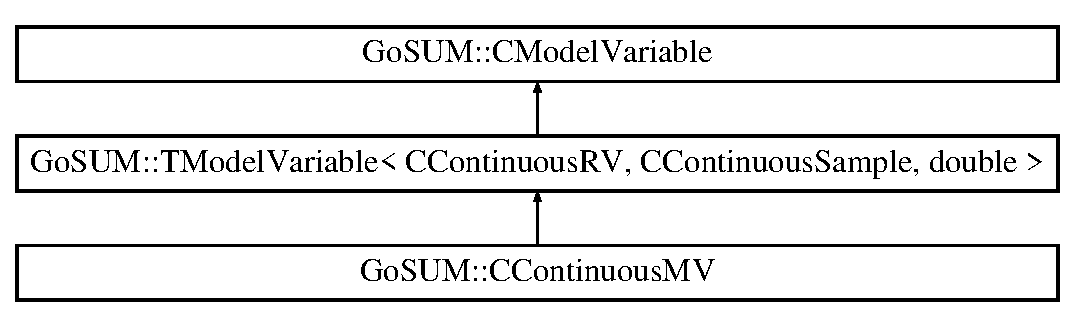
\includegraphics[height=3.000000cm]{class_go_s_u_m_1_1_c_continuous_m_v}
\end{center}
\end{figure}
\subsection*{Public Member Functions}
\begin{DoxyCompactItemize}
\item 
\hyperlink{class_go_s_u_m_1_1_c_continuous_m_v_a2ae3981f3aa32aea3c1d3224c31f4643}{C\-Continuous\-M\-V} (const std\-::string \&\-\_\-uname, \hyperlink{class_c_random_variable_a80d2a87c43847274138b51f7d713d7f1}{C\-Random\-Variable\-::distributiontype} \-\_\-type)
\begin{DoxyCompactList}\small\item\em Constructs new model variable by name and type. \end{DoxyCompactList}\item 
\hyperlink{class_go_s_u_m_1_1_c_continuous_m_v_a6934633087f0189586c9c5b7cb5f86f7}{C\-Continuous\-M\-V} (const \hyperlink{class_go_s_u_m_1_1_c_continuous_m_v}{C\-Continuous\-M\-V} \&O)
\item 
virtual void \hyperlink{class_go_s_u_m_1_1_c_continuous_m_v_a923c07b0735783d016b4e155b5eb0539}{set\-Theoretical\-Distribution} ()
\begin{DoxyCompactList}\small\item\em Tests goodness-\/of-\/fit for theoretical random variables and replaces with the best that satisfies Kolomogorov-\/\-Smirnov. \end{DoxyCompactList}\item 
virtual void \hyperlink{class_go_s_u_m_1_1_c_continuous_m_v_a65b0b9b16980f16fe2bc36bf8d79e3b9}{set\-Empirical\-Distribution} ()
\begin{DoxyCompactList}\small\item\em Compute distribution of the actual random variable from empirical sample data. \end{DoxyCompactList}\item 
virtual bool \hyperlink{class_go_s_u_m_1_1_c_continuous_m_v_a8f523f36ccdecfb58d468b6976890b15}{is\-Continuous} () const 
\begin{DoxyCompactList}\small\item\em Returns true if model variable is continuous, false otherwise. \end{DoxyCompactList}\item 
virtual bool \hyperlink{class_go_s_u_m_1_1_c_continuous_m_v_aeaef5939c27a7e074c33f783d73484a5}{is\-Discrete} () const 
\begin{DoxyCompactList}\small\item\em Returns true if model variable is discrete, false otherwise. \end{DoxyCompactList}\item 
bool \hyperlink{class_go_s_u_m_1_1_c_continuous_m_v_a58012df86509e7f8ee5b23c5e44b8465}{has\-Discrete\-Data} ()
\end{DoxyCompactItemize}
\subsection*{Private Member Functions}
\begin{DoxyCompactItemize}
\item 
{\footnotesize template$<$class Archive $>$ }\\void \hyperlink{class_go_s_u_m_1_1_c_continuous_m_v_a81cec49f19a1032334fdd57e7a61bdea}{serialize} (Archive \&ar, const unsigned int version)
\item 
\hyperlink{class_go_s_u_m_1_1_c_continuous_m_v_a74bd14dccc63f842fdc2e43fae3afde8}{C\-Continuous\-M\-V} ()
\begin{DoxyCompactList}\small\item\em Private constructor. \end{DoxyCompactList}\end{DoxyCompactItemize}
\subsection*{Friends}
\begin{DoxyCompactItemize}
\item 
class \hyperlink{class_go_s_u_m_1_1_c_continuous_m_v_ac98d07dd8f7b70e16ccb9a01abf56b9c}{boost\-::serialization\-::access}
\begin{DoxyCompactList}\small\item\em Boost serialization. \end{DoxyCompactList}\end{DoxyCompactItemize}
\subsection*{Additional Inherited Members}


\subsection{Constructor \& Destructor Documentation}
\hypertarget{class_go_s_u_m_1_1_c_continuous_m_v_a74bd14dccc63f842fdc2e43fae3afde8}{\index{Go\-S\-U\-M\-::\-C\-Continuous\-M\-V@{Go\-S\-U\-M\-::\-C\-Continuous\-M\-V}!C\-Continuous\-M\-V@{C\-Continuous\-M\-V}}
\index{C\-Continuous\-M\-V@{C\-Continuous\-M\-V}!GoSUM::CContinuousMV@{Go\-S\-U\-M\-::\-C\-Continuous\-M\-V}}
\subsubsection[{C\-Continuous\-M\-V}]{\setlength{\rightskip}{0pt plus 5cm}Go\-S\-U\-M\-::\-C\-Continuous\-M\-V\-::\-C\-Continuous\-M\-V (
\begin{DoxyParamCaption}
{}
\end{DoxyParamCaption}
)\hspace{0.3cm}{\ttfamily [inline]}, {\ttfamily [private]}}}\label{class_go_s_u_m_1_1_c_continuous_m_v_a74bd14dccc63f842fdc2e43fae3afde8}


Private constructor. 

\hypertarget{class_go_s_u_m_1_1_c_continuous_m_v_a2ae3981f3aa32aea3c1d3224c31f4643}{\index{Go\-S\-U\-M\-::\-C\-Continuous\-M\-V@{Go\-S\-U\-M\-::\-C\-Continuous\-M\-V}!C\-Continuous\-M\-V@{C\-Continuous\-M\-V}}
\index{C\-Continuous\-M\-V@{C\-Continuous\-M\-V}!GoSUM::CContinuousMV@{Go\-S\-U\-M\-::\-C\-Continuous\-M\-V}}
\subsubsection[{C\-Continuous\-M\-V}]{\setlength{\rightskip}{0pt plus 5cm}Go\-S\-U\-M\-::\-C\-Continuous\-M\-V\-::\-C\-Continuous\-M\-V (
\begin{DoxyParamCaption}
\item[{const std\-::string \&}]{\-\_\-uname, }
\item[{{\bf C\-Random\-Variable\-::distributiontype}}]{\-\_\-type}
\end{DoxyParamCaption}
)}}\label{class_go_s_u_m_1_1_c_continuous_m_v_a2ae3981f3aa32aea3c1d3224c31f4643}


Constructs new model variable by name and type. 

\hypertarget{class_go_s_u_m_1_1_c_continuous_m_v_a6934633087f0189586c9c5b7cb5f86f7}{\index{Go\-S\-U\-M\-::\-C\-Continuous\-M\-V@{Go\-S\-U\-M\-::\-C\-Continuous\-M\-V}!C\-Continuous\-M\-V@{C\-Continuous\-M\-V}}
\index{C\-Continuous\-M\-V@{C\-Continuous\-M\-V}!GoSUM::CContinuousMV@{Go\-S\-U\-M\-::\-C\-Continuous\-M\-V}}
\subsubsection[{C\-Continuous\-M\-V}]{\setlength{\rightskip}{0pt plus 5cm}Go\-S\-U\-M\-::\-C\-Continuous\-M\-V\-::\-C\-Continuous\-M\-V (
\begin{DoxyParamCaption}
\item[{const {\bf C\-Continuous\-M\-V} \&}]{O}
\end{DoxyParamCaption}
)}}\label{class_go_s_u_m_1_1_c_continuous_m_v_a6934633087f0189586c9c5b7cb5f86f7}


\subsection{Member Function Documentation}
\hypertarget{class_go_s_u_m_1_1_c_continuous_m_v_a58012df86509e7f8ee5b23c5e44b8465}{\index{Go\-S\-U\-M\-::\-C\-Continuous\-M\-V@{Go\-S\-U\-M\-::\-C\-Continuous\-M\-V}!has\-Discrete\-Data@{has\-Discrete\-Data}}
\index{has\-Discrete\-Data@{has\-Discrete\-Data}!GoSUM::CContinuousMV@{Go\-S\-U\-M\-::\-C\-Continuous\-M\-V}}
\subsubsection[{has\-Discrete\-Data}]{\setlength{\rightskip}{0pt plus 5cm}bool Go\-S\-U\-M\-::\-C\-Continuous\-M\-V\-::has\-Discrete\-Data (
\begin{DoxyParamCaption}
{}
\end{DoxyParamCaption}
)\hspace{0.3cm}{\ttfamily [inline]}}}\label{class_go_s_u_m_1_1_c_continuous_m_v_a58012df86509e7f8ee5b23c5e44b8465}
\hypertarget{class_go_s_u_m_1_1_c_continuous_m_v_a8f523f36ccdecfb58d468b6976890b15}{\index{Go\-S\-U\-M\-::\-C\-Continuous\-M\-V@{Go\-S\-U\-M\-::\-C\-Continuous\-M\-V}!is\-Continuous@{is\-Continuous}}
\index{is\-Continuous@{is\-Continuous}!GoSUM::CContinuousMV@{Go\-S\-U\-M\-::\-C\-Continuous\-M\-V}}
\subsubsection[{is\-Continuous}]{\setlength{\rightskip}{0pt plus 5cm}virtual bool Go\-S\-U\-M\-::\-C\-Continuous\-M\-V\-::is\-Continuous (
\begin{DoxyParamCaption}
{}
\end{DoxyParamCaption}
) const\hspace{0.3cm}{\ttfamily [inline]}, {\ttfamily [virtual]}}}\label{class_go_s_u_m_1_1_c_continuous_m_v_a8f523f36ccdecfb58d468b6976890b15}


Returns true if model variable is continuous, false otherwise. 



Implements \hyperlink{class_go_s_u_m_1_1_c_model_variable_a2ec4aee717249dcbad98fd6e6320a6b7}{Go\-S\-U\-M\-::\-C\-Model\-Variable}.

\hypertarget{class_go_s_u_m_1_1_c_continuous_m_v_aeaef5939c27a7e074c33f783d73484a5}{\index{Go\-S\-U\-M\-::\-C\-Continuous\-M\-V@{Go\-S\-U\-M\-::\-C\-Continuous\-M\-V}!is\-Discrete@{is\-Discrete}}
\index{is\-Discrete@{is\-Discrete}!GoSUM::CContinuousMV@{Go\-S\-U\-M\-::\-C\-Continuous\-M\-V}}
\subsubsection[{is\-Discrete}]{\setlength{\rightskip}{0pt plus 5cm}virtual bool Go\-S\-U\-M\-::\-C\-Continuous\-M\-V\-::is\-Discrete (
\begin{DoxyParamCaption}
{}
\end{DoxyParamCaption}
) const\hspace{0.3cm}{\ttfamily [inline]}, {\ttfamily [virtual]}}}\label{class_go_s_u_m_1_1_c_continuous_m_v_aeaef5939c27a7e074c33f783d73484a5}


Returns true if model variable is discrete, false otherwise. 



Implements \hyperlink{class_go_s_u_m_1_1_c_model_variable_a9d0140b610b7a1c04a3b31e2d84f86da}{Go\-S\-U\-M\-::\-C\-Model\-Variable}.

\hypertarget{class_go_s_u_m_1_1_c_continuous_m_v_a81cec49f19a1032334fdd57e7a61bdea}{\index{Go\-S\-U\-M\-::\-C\-Continuous\-M\-V@{Go\-S\-U\-M\-::\-C\-Continuous\-M\-V}!serialize@{serialize}}
\index{serialize@{serialize}!GoSUM::CContinuousMV@{Go\-S\-U\-M\-::\-C\-Continuous\-M\-V}}
\subsubsection[{serialize}]{\setlength{\rightskip}{0pt plus 5cm}template$<$class Archive $>$ void Go\-S\-U\-M\-::\-C\-Continuous\-M\-V\-::serialize (
\begin{DoxyParamCaption}
\item[{Archive \&}]{ar, }
\item[{const unsigned int}]{version}
\end{DoxyParamCaption}
)\hspace{0.3cm}{\ttfamily [inline]}, {\ttfamily [private]}}}\label{class_go_s_u_m_1_1_c_continuous_m_v_a81cec49f19a1032334fdd57e7a61bdea}
\hypertarget{class_go_s_u_m_1_1_c_continuous_m_v_a65b0b9b16980f16fe2bc36bf8d79e3b9}{\index{Go\-S\-U\-M\-::\-C\-Continuous\-M\-V@{Go\-S\-U\-M\-::\-C\-Continuous\-M\-V}!set\-Empirical\-Distribution@{set\-Empirical\-Distribution}}
\index{set\-Empirical\-Distribution@{set\-Empirical\-Distribution}!GoSUM::CContinuousMV@{Go\-S\-U\-M\-::\-C\-Continuous\-M\-V}}
\subsubsection[{set\-Empirical\-Distribution}]{\setlength{\rightskip}{0pt plus 5cm}virtual void Go\-S\-U\-M\-::\-C\-Continuous\-M\-V\-::set\-Empirical\-Distribution (
\begin{DoxyParamCaption}
{}
\end{DoxyParamCaption}
)\hspace{0.3cm}{\ttfamily [inline]}, {\ttfamily [virtual]}}}\label{class_go_s_u_m_1_1_c_continuous_m_v_a65b0b9b16980f16fe2bc36bf8d79e3b9}


Compute distribution of the actual random variable from empirical sample data. 



Implements \hyperlink{class_go_s_u_m_1_1_t_model_variable_a3128d12e3ce0757714a7596de087314e}{Go\-S\-U\-M\-::\-T\-Model\-Variable$<$ R, S, t $>$}.

\hypertarget{class_go_s_u_m_1_1_c_continuous_m_v_a923c07b0735783d016b4e155b5eb0539}{\index{Go\-S\-U\-M\-::\-C\-Continuous\-M\-V@{Go\-S\-U\-M\-::\-C\-Continuous\-M\-V}!set\-Theoretical\-Distribution@{set\-Theoretical\-Distribution}}
\index{set\-Theoretical\-Distribution@{set\-Theoretical\-Distribution}!GoSUM::CContinuousMV@{Go\-S\-U\-M\-::\-C\-Continuous\-M\-V}}
\subsubsection[{set\-Theoretical\-Distribution}]{\setlength{\rightskip}{0pt plus 5cm}void Go\-S\-U\-M\-::\-C\-Continuous\-M\-V\-::set\-Theoretical\-Distribution (
\begin{DoxyParamCaption}
{}
\end{DoxyParamCaption}
)\hspace{0.3cm}{\ttfamily [virtual]}}}\label{class_go_s_u_m_1_1_c_continuous_m_v_a923c07b0735783d016b4e155b5eb0539}


Tests goodness-\/of-\/fit for theoretical random variables and replaces with the best that satisfies Kolomogorov-\/\-Smirnov. 



Implements \hyperlink{class_go_s_u_m_1_1_t_model_variable_ad113f33f216796f775855dd3f8553f03}{Go\-S\-U\-M\-::\-T\-Model\-Variable$<$ R, S, t $>$}.



\subsection{Friends And Related Function Documentation}
\hypertarget{class_go_s_u_m_1_1_c_continuous_m_v_ac98d07dd8f7b70e16ccb9a01abf56b9c}{\index{Go\-S\-U\-M\-::\-C\-Continuous\-M\-V@{Go\-S\-U\-M\-::\-C\-Continuous\-M\-V}!boost\-::serialization\-::access@{boost\-::serialization\-::access}}
\index{boost\-::serialization\-::access@{boost\-::serialization\-::access}!GoSUM::CContinuousMV@{Go\-S\-U\-M\-::\-C\-Continuous\-M\-V}}
\subsubsection[{boost\-::serialization\-::access}]{\setlength{\rightskip}{0pt plus 5cm}friend class boost\-::serialization\-::access\hspace{0.3cm}{\ttfamily [friend]}}}\label{class_go_s_u_m_1_1_c_continuous_m_v_ac98d07dd8f7b70e16ccb9a01abf56b9c}


Boost serialization. 



The documentation for this class was generated from the following files\-:\begin{DoxyCompactItemize}
\item 
C\-:/\-Development/core/\hyperlink{_model_variable_8h}{Model\-Variable.\-h}\item 
C\-:/\-Development/core/\hyperlink{_model_variable_8cpp}{Model\-Variable.\-cpp}\end{DoxyCompactItemize}

\hypertarget{class_c_continuous_r_v}{\section{C\-Continuous\-R\-V Class Reference}
\label{class_c_continuous_r_v}\index{C\-Continuous\-R\-V@{C\-Continuous\-R\-V}}
}


{\ttfamily \#include $<$Random\-Variable.\-h$>$}

Inheritance diagram for C\-Continuous\-R\-V\-:\begin{figure}[H]
\begin{center}
\leavevmode
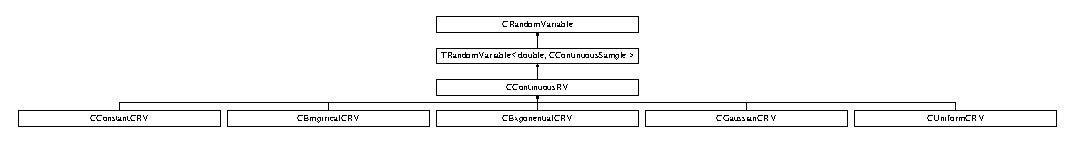
\includegraphics[height=1.473684cm]{class_c_continuous_r_v}
\end{center}
\end{figure}
\subsection*{Public Member Functions}
\begin{DoxyCompactItemize}
\item 
\hyperlink{class_c_continuous_r_v_a3501c35710b9b8dea56976f2fb895a20}{C\-Continuous\-R\-V} ()
\item 
\hyperlink{class_c_continuous_r_v_a1b0b4cedcbfa308f76ebc71df0cc4429}{C\-Continuous\-R\-V} (const \hyperlink{class_c_continuous_r_v}{C\-Continuous\-R\-V} \&O)
\item 
double \hyperlink{class_c_continuous_r_v_a4cfd8083c22c2283e9246652a2f79686}{probability} (double \-\_\-x1, double \-\_\-x2) const 
\begin{DoxyCompactList}\small\item\em Returns probablilty that random variable has value between \-\_\-x1 and \-\_\-x2. \end{DoxyCompactList}\item 
virtual double \hyperlink{class_c_continuous_r_v_a14207c5f0664f1a5436acd44a21ce46f}{quantile} (double \-\_\-p) const 
\begin{DoxyCompactList}\small\item\em Quantile, only argument checking. \end{DoxyCompactList}\end{DoxyCompactItemize}
\subsection*{Private Member Functions}
\begin{DoxyCompactItemize}
\item 
{\footnotesize template$<$class Archive $>$ }\\void \hyperlink{class_c_continuous_r_v_a6de70e5300ddf0f1d1ab71e568b971e0}{serialize} (Archive \&ar, const unsigned int version)
\end{DoxyCompactItemize}
\subsection*{Friends}
\begin{DoxyCompactItemize}
\item 
class \hyperlink{class_c_continuous_r_v_ac98d07dd8f7b70e16ccb9a01abf56b9c}{boost\-::serialization\-::access}
\begin{DoxyCompactList}\small\item\em Boost serialization. \end{DoxyCompactList}\end{DoxyCompactItemize}
\subsection*{Additional Inherited Members}


\subsection{Constructor \& Destructor Documentation}
\hypertarget{class_c_continuous_r_v_a3501c35710b9b8dea56976f2fb895a20}{\index{C\-Continuous\-R\-V@{C\-Continuous\-R\-V}!C\-Continuous\-R\-V@{C\-Continuous\-R\-V}}
\index{C\-Continuous\-R\-V@{C\-Continuous\-R\-V}!CContinuousRV@{C\-Continuous\-R\-V}}
\subsubsection[{C\-Continuous\-R\-V}]{\setlength{\rightskip}{0pt plus 5cm}C\-Continuous\-R\-V\-::\-C\-Continuous\-R\-V (
\begin{DoxyParamCaption}
{}
\end{DoxyParamCaption}
)\hspace{0.3cm}{\ttfamily [inline]}}}\label{class_c_continuous_r_v_a3501c35710b9b8dea56976f2fb895a20}
\hypertarget{class_c_continuous_r_v_a1b0b4cedcbfa308f76ebc71df0cc4429}{\index{C\-Continuous\-R\-V@{C\-Continuous\-R\-V}!C\-Continuous\-R\-V@{C\-Continuous\-R\-V}}
\index{C\-Continuous\-R\-V@{C\-Continuous\-R\-V}!CContinuousRV@{C\-Continuous\-R\-V}}
\subsubsection[{C\-Continuous\-R\-V}]{\setlength{\rightskip}{0pt plus 5cm}C\-Continuous\-R\-V\-::\-C\-Continuous\-R\-V (
\begin{DoxyParamCaption}
\item[{const {\bf C\-Continuous\-R\-V} \&}]{O}
\end{DoxyParamCaption}
)\hspace{0.3cm}{\ttfamily [inline]}}}\label{class_c_continuous_r_v_a1b0b4cedcbfa308f76ebc71df0cc4429}


\subsection{Member Function Documentation}
\hypertarget{class_c_continuous_r_v_a4cfd8083c22c2283e9246652a2f79686}{\index{C\-Continuous\-R\-V@{C\-Continuous\-R\-V}!probability@{probability}}
\index{probability@{probability}!CContinuousRV@{C\-Continuous\-R\-V}}
\subsubsection[{probability}]{\setlength{\rightskip}{0pt plus 5cm}double C\-Continuous\-R\-V\-::probability (
\begin{DoxyParamCaption}
\item[{double}]{\-\_\-x1, }
\item[{double}]{\-\_\-x2}
\end{DoxyParamCaption}
) const\hspace{0.3cm}{\ttfamily [inline]}}}\label{class_c_continuous_r_v_a4cfd8083c22c2283e9246652a2f79686}


Returns probablilty that random variable has value between \-\_\-x1 and \-\_\-x2. 

\hypertarget{class_c_continuous_r_v_a14207c5f0664f1a5436acd44a21ce46f}{\index{C\-Continuous\-R\-V@{C\-Continuous\-R\-V}!quantile@{quantile}}
\index{quantile@{quantile}!CContinuousRV@{C\-Continuous\-R\-V}}
\subsubsection[{quantile}]{\setlength{\rightskip}{0pt plus 5cm}virtual double C\-Continuous\-R\-V\-::quantile (
\begin{DoxyParamCaption}
\item[{double}]{\-\_\-p}
\end{DoxyParamCaption}
) const\hspace{0.3cm}{\ttfamily [inline]}, {\ttfamily [virtual]}}}\label{class_c_continuous_r_v_a14207c5f0664f1a5436acd44a21ce46f}


Quantile, only argument checking. 



Implements \hyperlink{class_c_random_variable_aad8f00777fdad0e7e1ad29c9ea620ff2}{C\-Random\-Variable}.

\hypertarget{class_c_continuous_r_v_a6de70e5300ddf0f1d1ab71e568b971e0}{\index{C\-Continuous\-R\-V@{C\-Continuous\-R\-V}!serialize@{serialize}}
\index{serialize@{serialize}!CContinuousRV@{C\-Continuous\-R\-V}}
\subsubsection[{serialize}]{\setlength{\rightskip}{0pt plus 5cm}template$<$class Archive $>$ void C\-Continuous\-R\-V\-::serialize (
\begin{DoxyParamCaption}
\item[{Archive \&}]{ar, }
\item[{const unsigned int}]{version}
\end{DoxyParamCaption}
)\hspace{0.3cm}{\ttfamily [inline]}, {\ttfamily [private]}}}\label{class_c_continuous_r_v_a6de70e5300ddf0f1d1ab71e568b971e0}


\subsection{Friends And Related Function Documentation}
\hypertarget{class_c_continuous_r_v_ac98d07dd8f7b70e16ccb9a01abf56b9c}{\index{C\-Continuous\-R\-V@{C\-Continuous\-R\-V}!boost\-::serialization\-::access@{boost\-::serialization\-::access}}
\index{boost\-::serialization\-::access@{boost\-::serialization\-::access}!CContinuousRV@{C\-Continuous\-R\-V}}
\subsubsection[{boost\-::serialization\-::access}]{\setlength{\rightskip}{0pt plus 5cm}friend class boost\-::serialization\-::access\hspace{0.3cm}{\ttfamily [friend]}}}\label{class_c_continuous_r_v_ac98d07dd8f7b70e16ccb9a01abf56b9c}


Boost serialization. 



The documentation for this class was generated from the following file\-:\begin{DoxyCompactItemize}
\item 
C\-:/\-Development/core/\hyperlink{_random_variable_8h}{Random\-Variable.\-h}\end{DoxyCompactItemize}

\hypertarget{class_c_continuous_sample}{\section{C\-Continuous\-Sample Class Reference}
\label{class_c_continuous_sample}\index{C\-Continuous\-Sample@{C\-Continuous\-Sample}}
}


{\ttfamily \#include $<$Sample.\-h$>$}

Inheritance diagram for C\-Continuous\-Sample\-:\begin{figure}[H]
\begin{center}
\leavevmode
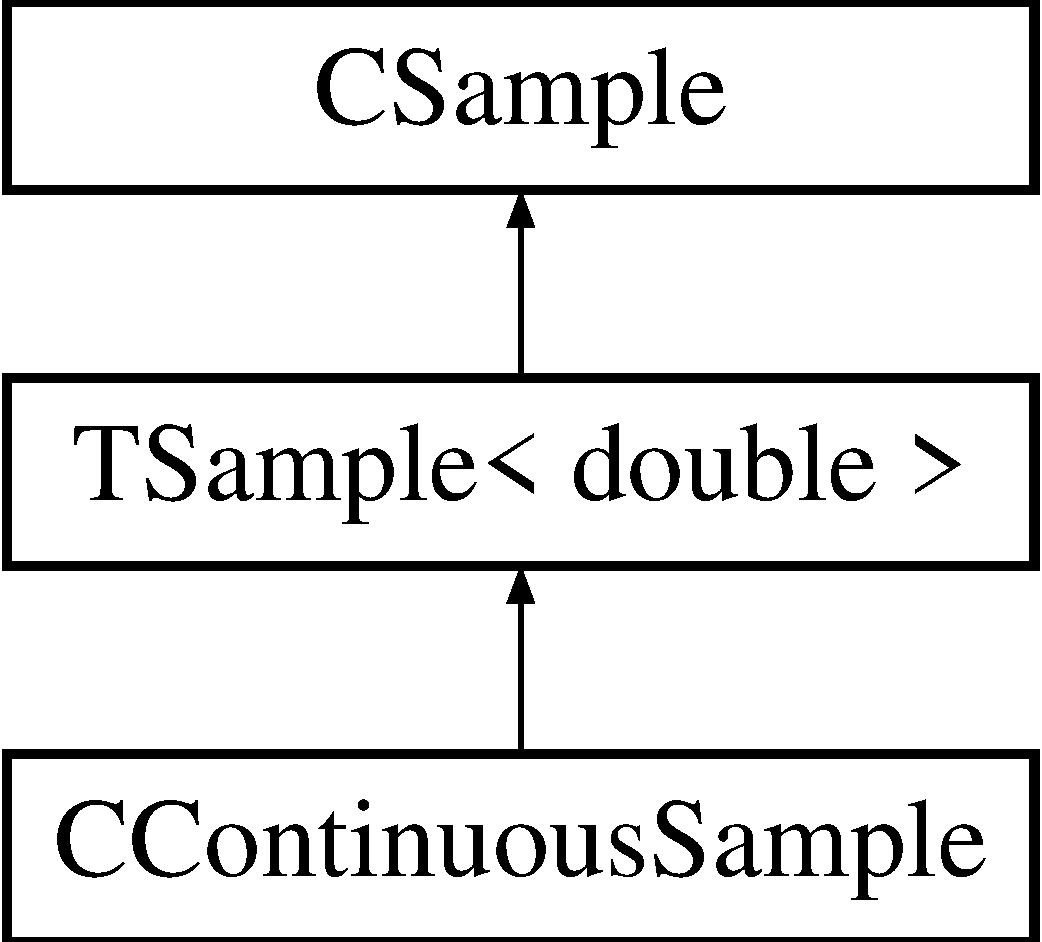
\includegraphics[height=3.000000cm]{class_c_continuous_sample}
\end{center}
\end{figure}
\subsection*{Public Member Functions}
\begin{DoxyCompactItemize}
\item 
\hyperlink{class_c_continuous_sample_ada43d66e4e4e38cfa8c82e55d618a614}{C\-Continuous\-Sample} ()
\item 
virtual \hyperlink{class_c_continuous_sample_af7732d71f3a91df8941993dc22f62d0a}{$\sim$\-C\-Continuous\-Sample} ()
\item 
\hyperlink{class_c_continuous_sample_aaefe6f714c1f0b6907ae3c443fff34b0}{C\-Continuous\-Sample} (const \hyperlink{class_c_continuous_sample}{C\-Continuous\-Sample} \&O)
\item 
virtual void \hyperlink{class_c_continuous_sample_aed08dc4372c437b9a6168399f583d863}{compute\-Statistics} (int \-\_\-n)
\begin{DoxyCompactList}\small\item\em Computes sample statistics, i.\-e. normalized histogram etc. \end{DoxyCompactList}\item 
virtual double \hyperlink{class_c_continuous_sample_a30e72f44dbb7c2ca3c6b8f77ff53688a}{mean} () const 
\begin{DoxyCompactList}\small\item\em Returns empirical mean. \end{DoxyCompactList}\item 
virtual double \hyperlink{class_c_continuous_sample_a676e1bdea044e64b6c096fd58d056116}{standard\-Deviation} () const 
\begin{DoxyCompactList}\small\item\em Returns empirical standard deviation. \end{DoxyCompactList}\item 
virtual double \hyperlink{class_c_continuous_sample_ad2011a526a7e7c156bdf7a9cccf48277}{export\-Histogram} (Array\-Xd \&\-\_\-x, Array\-Xd \&\-\_\-\-H) const 
\begin{DoxyCompactList}\small\item\em Exports histogram (x,H). \end{DoxyCompactList}\item 
virtual void \hyperlink{class_c_continuous_sample_aa3ea500b67bc9fdb767c7c324975a2eb}{export\-Sub\-Histogram} (Array\-Xd \&\-\_\-sub\-H, const std\-::vector$<$ int $>$ \&subset) const 
\begin{DoxyCompactList}\small\item\em Exports histogram relative to a subset of sample data. \end{DoxyCompactList}\item 
virtual double \hyperlink{class_c_continuous_sample_a79881662a2bcb842c97b418487d57eed}{variance} () const 
\begin{DoxyCompactList}\small\item\em Returns sample variance (i.\-e.\-empirical). \end{DoxyCompactList}\item 
bool \hyperlink{class_c_continuous_sample_a61a67310dfc13d836a845ec59cddd38e}{has\-Discrete\-Data} ()
\end{DoxyCompactItemize}
\subsection*{Protected Member Functions}
\begin{DoxyCompactItemize}
\item 
{\footnotesize template$<$class Archive $>$ }\\void \hyperlink{class_c_continuous_sample_ab5508a93778215d7408fde456f9e8faf}{serialize} (Archive \&ar, const unsigned int version)
\end{DoxyCompactItemize}
\subsection*{Protected Attributes}
\begin{DoxyCompactItemize}
\item 
double \hyperlink{class_c_continuous_sample_a1e4e0d9a75c4111d5c5c3bc67ded57bb}{mu}
\item 
double \hyperlink{class_c_continuous_sample_a5ccdb718bac3e945f5e593d0137717e0}{stdv}
\end{DoxyCompactItemize}
\subsection*{Private Member Functions}
\begin{DoxyCompactItemize}
\item 
virtual void \hyperlink{class_c_continuous_sample_a59be50a77a49716c8fd181c2c1eb10bd}{compute\-Normalized\-Histogram} (int \-\_\-n)
\begin{DoxyCompactList}\small\item\em Computes normalized histogram from sample data. \end{DoxyCompactList}\item 
virtual void \hyperlink{class_c_continuous_sample_a2d7208d5acb81d8d9e69e7c24a916d99}{compute\-Normalized\-Sub\-Histogram} (Array\-Xd \&\-\_\-sub\-H, const std\-::vector$<$ int $>$ \&subset) const 
\begin{DoxyCompactList}\small\item\em Computes normalized histogram from a subset of sample data. \end{DoxyCompactList}\item 
virtual void \hyperlink{class_c_continuous_sample_a50aa31aff2e9767744e74f9b482aa8c5}{compute\-Mean\-And\-Standard\-Deviation} ()
\begin{DoxyCompactList}\small\item\em Computes empirical mean and standard deviation. \end{DoxyCompactList}\end{DoxyCompactItemize}
\subsection*{Friends}
\begin{DoxyCompactItemize}
\item 
class \hyperlink{class_c_continuous_sample_ac98d07dd8f7b70e16ccb9a01abf56b9c}{boost\-::serialization\-::access}
\begin{DoxyCompactList}\small\item\em Boost serialization. \end{DoxyCompactList}\end{DoxyCompactItemize}
\subsection*{Additional Inherited Members}


\subsection{Constructor \& Destructor Documentation}
\hypertarget{class_c_continuous_sample_ada43d66e4e4e38cfa8c82e55d618a614}{\index{C\-Continuous\-Sample@{C\-Continuous\-Sample}!C\-Continuous\-Sample@{C\-Continuous\-Sample}}
\index{C\-Continuous\-Sample@{C\-Continuous\-Sample}!CContinuousSample@{C\-Continuous\-Sample}}
\subsubsection[{C\-Continuous\-Sample}]{\setlength{\rightskip}{0pt plus 5cm}C\-Continuous\-Sample\-::\-C\-Continuous\-Sample (
\begin{DoxyParamCaption}
{}
\end{DoxyParamCaption}
)\hspace{0.3cm}{\ttfamily [inline]}}}\label{class_c_continuous_sample_ada43d66e4e4e38cfa8c82e55d618a614}
\hypertarget{class_c_continuous_sample_af7732d71f3a91df8941993dc22f62d0a}{\index{C\-Continuous\-Sample@{C\-Continuous\-Sample}!$\sim$\-C\-Continuous\-Sample@{$\sim$\-C\-Continuous\-Sample}}
\index{$\sim$\-C\-Continuous\-Sample@{$\sim$\-C\-Continuous\-Sample}!CContinuousSample@{C\-Continuous\-Sample}}
\subsubsection[{$\sim$\-C\-Continuous\-Sample}]{\setlength{\rightskip}{0pt plus 5cm}virtual C\-Continuous\-Sample\-::$\sim$\-C\-Continuous\-Sample (
\begin{DoxyParamCaption}
{}
\end{DoxyParamCaption}
)\hspace{0.3cm}{\ttfamily [inline]}, {\ttfamily [virtual]}}}\label{class_c_continuous_sample_af7732d71f3a91df8941993dc22f62d0a}
\hypertarget{class_c_continuous_sample_aaefe6f714c1f0b6907ae3c443fff34b0}{\index{C\-Continuous\-Sample@{C\-Continuous\-Sample}!C\-Continuous\-Sample@{C\-Continuous\-Sample}}
\index{C\-Continuous\-Sample@{C\-Continuous\-Sample}!CContinuousSample@{C\-Continuous\-Sample}}
\subsubsection[{C\-Continuous\-Sample}]{\setlength{\rightskip}{0pt plus 5cm}C\-Continuous\-Sample\-::\-C\-Continuous\-Sample (
\begin{DoxyParamCaption}
\item[{const {\bf C\-Continuous\-Sample} \&}]{O}
\end{DoxyParamCaption}
)\hspace{0.3cm}{\ttfamily [inline]}}}\label{class_c_continuous_sample_aaefe6f714c1f0b6907ae3c443fff34b0}


\subsection{Member Function Documentation}
\hypertarget{class_c_continuous_sample_a50aa31aff2e9767744e74f9b482aa8c5}{\index{C\-Continuous\-Sample@{C\-Continuous\-Sample}!compute\-Mean\-And\-Standard\-Deviation@{compute\-Mean\-And\-Standard\-Deviation}}
\index{compute\-Mean\-And\-Standard\-Deviation@{compute\-Mean\-And\-Standard\-Deviation}!CContinuousSample@{C\-Continuous\-Sample}}
\subsubsection[{compute\-Mean\-And\-Standard\-Deviation}]{\setlength{\rightskip}{0pt plus 5cm}void C\-Continuous\-Sample\-::compute\-Mean\-And\-Standard\-Deviation (
\begin{DoxyParamCaption}
{}
\end{DoxyParamCaption}
)\hspace{0.3cm}{\ttfamily [private]}, {\ttfamily [virtual]}}}\label{class_c_continuous_sample_a50aa31aff2e9767744e74f9b482aa8c5}


Computes empirical mean and standard deviation. 

\hypertarget{class_c_continuous_sample_a59be50a77a49716c8fd181c2c1eb10bd}{\index{C\-Continuous\-Sample@{C\-Continuous\-Sample}!compute\-Normalized\-Histogram@{compute\-Normalized\-Histogram}}
\index{compute\-Normalized\-Histogram@{compute\-Normalized\-Histogram}!CContinuousSample@{C\-Continuous\-Sample}}
\subsubsection[{compute\-Normalized\-Histogram}]{\setlength{\rightskip}{0pt plus 5cm}void C\-Continuous\-Sample\-::compute\-Normalized\-Histogram (
\begin{DoxyParamCaption}
\item[{int}]{\-\_\-n}
\end{DoxyParamCaption}
)\hspace{0.3cm}{\ttfamily [private]}, {\ttfamily [virtual]}}}\label{class_c_continuous_sample_a59be50a77a49716c8fd181c2c1eb10bd}


Computes normalized histogram from sample data. 

\hypertarget{class_c_continuous_sample_a2d7208d5acb81d8d9e69e7c24a916d99}{\index{C\-Continuous\-Sample@{C\-Continuous\-Sample}!compute\-Normalized\-Sub\-Histogram@{compute\-Normalized\-Sub\-Histogram}}
\index{compute\-Normalized\-Sub\-Histogram@{compute\-Normalized\-Sub\-Histogram}!CContinuousSample@{C\-Continuous\-Sample}}
\subsubsection[{compute\-Normalized\-Sub\-Histogram}]{\setlength{\rightskip}{0pt plus 5cm}void C\-Continuous\-Sample\-::compute\-Normalized\-Sub\-Histogram (
\begin{DoxyParamCaption}
\item[{Array\-Xd \&}]{\-\_\-sub\-H, }
\item[{const std\-::vector$<$ int $>$ \&}]{subset}
\end{DoxyParamCaption}
) const\hspace{0.3cm}{\ttfamily [private]}, {\ttfamily [virtual]}}}\label{class_c_continuous_sample_a2d7208d5acb81d8d9e69e7c24a916d99}


Computes normalized histogram from a subset of sample data. 

\hypertarget{class_c_continuous_sample_aed08dc4372c437b9a6168399f583d863}{\index{C\-Continuous\-Sample@{C\-Continuous\-Sample}!compute\-Statistics@{compute\-Statistics}}
\index{compute\-Statistics@{compute\-Statistics}!CContinuousSample@{C\-Continuous\-Sample}}
\subsubsection[{compute\-Statistics}]{\setlength{\rightskip}{0pt plus 5cm}virtual void C\-Continuous\-Sample\-::compute\-Statistics (
\begin{DoxyParamCaption}
\item[{int}]{\-\_\-n}
\end{DoxyParamCaption}
)\hspace{0.3cm}{\ttfamily [inline]}, {\ttfamily [virtual]}}}\label{class_c_continuous_sample_aed08dc4372c437b9a6168399f583d863}


Computes sample statistics, i.\-e. normalized histogram etc. 



Implements \hyperlink{class_c_sample_a10000ec1dade335a2a96a8646e0bae03}{C\-Sample}.

\hypertarget{class_c_continuous_sample_ad2011a526a7e7c156bdf7a9cccf48277}{\index{C\-Continuous\-Sample@{C\-Continuous\-Sample}!export\-Histogram@{export\-Histogram}}
\index{export\-Histogram@{export\-Histogram}!CContinuousSample@{C\-Continuous\-Sample}}
\subsubsection[{export\-Histogram}]{\setlength{\rightskip}{0pt plus 5cm}double C\-Continuous\-Sample\-::export\-Histogram (
\begin{DoxyParamCaption}
\item[{Array\-Xd \&}]{\-\_\-x, }
\item[{Array\-Xd \&}]{\-\_\-\-H}
\end{DoxyParamCaption}
) const\hspace{0.3cm}{\ttfamily [virtual]}}}\label{class_c_continuous_sample_ad2011a526a7e7c156bdf7a9cccf48277}


Exports histogram (x,H). 

\hypertarget{class_c_continuous_sample_aa3ea500b67bc9fdb767c7c324975a2eb}{\index{C\-Continuous\-Sample@{C\-Continuous\-Sample}!export\-Sub\-Histogram@{export\-Sub\-Histogram}}
\index{export\-Sub\-Histogram@{export\-Sub\-Histogram}!CContinuousSample@{C\-Continuous\-Sample}}
\subsubsection[{export\-Sub\-Histogram}]{\setlength{\rightskip}{0pt plus 5cm}void C\-Continuous\-Sample\-::export\-Sub\-Histogram (
\begin{DoxyParamCaption}
\item[{Array\-Xd \&}]{\-\_\-sub\-H, }
\item[{const std\-::vector$<$ int $>$ \&}]{subset}
\end{DoxyParamCaption}
) const\hspace{0.3cm}{\ttfamily [virtual]}}}\label{class_c_continuous_sample_aa3ea500b67bc9fdb767c7c324975a2eb}


Exports histogram relative to a subset of sample data. 



Implements \hyperlink{class_t_sample_a1ce3bdd77627f5783edbec6f607c3ea9}{T\-Sample$<$ t $>$}.

\hypertarget{class_c_continuous_sample_a61a67310dfc13d836a845ec59cddd38e}{\index{C\-Continuous\-Sample@{C\-Continuous\-Sample}!has\-Discrete\-Data@{has\-Discrete\-Data}}
\index{has\-Discrete\-Data@{has\-Discrete\-Data}!CContinuousSample@{C\-Continuous\-Sample}}
\subsubsection[{has\-Discrete\-Data}]{\setlength{\rightskip}{0pt plus 5cm}bool C\-Continuous\-Sample\-::has\-Discrete\-Data (
\begin{DoxyParamCaption}
{}
\end{DoxyParamCaption}
)}}\label{class_c_continuous_sample_a61a67310dfc13d836a845ec59cddd38e}
\hypertarget{class_c_continuous_sample_a30e72f44dbb7c2ca3c6b8f77ff53688a}{\index{C\-Continuous\-Sample@{C\-Continuous\-Sample}!mean@{mean}}
\index{mean@{mean}!CContinuousSample@{C\-Continuous\-Sample}}
\subsubsection[{mean}]{\setlength{\rightskip}{0pt plus 5cm}virtual double C\-Continuous\-Sample\-::mean (
\begin{DoxyParamCaption}
{}
\end{DoxyParamCaption}
) const\hspace{0.3cm}{\ttfamily [inline]}, {\ttfamily [virtual]}}}\label{class_c_continuous_sample_a30e72f44dbb7c2ca3c6b8f77ff53688a}


Returns empirical mean. 

\hypertarget{class_c_continuous_sample_ab5508a93778215d7408fde456f9e8faf}{\index{C\-Continuous\-Sample@{C\-Continuous\-Sample}!serialize@{serialize}}
\index{serialize@{serialize}!CContinuousSample@{C\-Continuous\-Sample}}
\subsubsection[{serialize}]{\setlength{\rightskip}{0pt plus 5cm}template$<$class Archive $>$ void C\-Continuous\-Sample\-::serialize (
\begin{DoxyParamCaption}
\item[{Archive \&}]{ar, }
\item[{const unsigned int}]{version}
\end{DoxyParamCaption}
)\hspace{0.3cm}{\ttfamily [protected]}}}\label{class_c_continuous_sample_ab5508a93778215d7408fde456f9e8faf}


Reimplemented from \hyperlink{class_t_sample_a0f53b1db72dd3e83c50ab28dd31929a5}{T\-Sample$<$ t $>$}.

\hypertarget{class_c_continuous_sample_a676e1bdea044e64b6c096fd58d056116}{\index{C\-Continuous\-Sample@{C\-Continuous\-Sample}!standard\-Deviation@{standard\-Deviation}}
\index{standard\-Deviation@{standard\-Deviation}!CContinuousSample@{C\-Continuous\-Sample}}
\subsubsection[{standard\-Deviation}]{\setlength{\rightskip}{0pt plus 5cm}virtual double C\-Continuous\-Sample\-::standard\-Deviation (
\begin{DoxyParamCaption}
{}
\end{DoxyParamCaption}
) const\hspace{0.3cm}{\ttfamily [inline]}, {\ttfamily [virtual]}}}\label{class_c_continuous_sample_a676e1bdea044e64b6c096fd58d056116}


Returns empirical standard deviation. 

\hypertarget{class_c_continuous_sample_a79881662a2bcb842c97b418487d57eed}{\index{C\-Continuous\-Sample@{C\-Continuous\-Sample}!variance@{variance}}
\index{variance@{variance}!CContinuousSample@{C\-Continuous\-Sample}}
\subsubsection[{variance}]{\setlength{\rightskip}{0pt plus 5cm}virtual double C\-Continuous\-Sample\-::variance (
\begin{DoxyParamCaption}
{}
\end{DoxyParamCaption}
) const\hspace{0.3cm}{\ttfamily [inline]}, {\ttfamily [virtual]}}}\label{class_c_continuous_sample_a79881662a2bcb842c97b418487d57eed}


Returns sample variance (i.\-e.\-empirical). 



Implements \hyperlink{class_c_sample_a5ce1e4ff44a8ac2e021dc36541343651}{C\-Sample}.



\subsection{Friends And Related Function Documentation}
\hypertarget{class_c_continuous_sample_ac98d07dd8f7b70e16ccb9a01abf56b9c}{\index{C\-Continuous\-Sample@{C\-Continuous\-Sample}!boost\-::serialization\-::access@{boost\-::serialization\-::access}}
\index{boost\-::serialization\-::access@{boost\-::serialization\-::access}!CContinuousSample@{C\-Continuous\-Sample}}
\subsubsection[{boost\-::serialization\-::access}]{\setlength{\rightskip}{0pt plus 5cm}friend class boost\-::serialization\-::access\hspace{0.3cm}{\ttfamily [friend]}}}\label{class_c_continuous_sample_ac98d07dd8f7b70e16ccb9a01abf56b9c}


Boost serialization. 



\subsection{Member Data Documentation}
\hypertarget{class_c_continuous_sample_a1e4e0d9a75c4111d5c5c3bc67ded57bb}{\index{C\-Continuous\-Sample@{C\-Continuous\-Sample}!mu@{mu}}
\index{mu@{mu}!CContinuousSample@{C\-Continuous\-Sample}}
\subsubsection[{mu}]{\setlength{\rightskip}{0pt plus 5cm}double C\-Continuous\-Sample\-::mu\hspace{0.3cm}{\ttfamily [protected]}}}\label{class_c_continuous_sample_a1e4e0d9a75c4111d5c5c3bc67ded57bb}
\hypertarget{class_c_continuous_sample_a5ccdb718bac3e945f5e593d0137717e0}{\index{C\-Continuous\-Sample@{C\-Continuous\-Sample}!stdv@{stdv}}
\index{stdv@{stdv}!CContinuousSample@{C\-Continuous\-Sample}}
\subsubsection[{stdv}]{\setlength{\rightskip}{0pt plus 5cm}double C\-Continuous\-Sample\-::stdv\hspace{0.3cm}{\ttfamily [protected]}}}\label{class_c_continuous_sample_a5ccdb718bac3e945f5e593d0137717e0}
Empirical mean (mu) and standard deviation (std). 

The documentation for this class was generated from the following files\-:\begin{DoxyCompactItemize}
\item 
C\-:/\-Development/core/\hyperlink{_sample_8h}{Sample.\-h}\item 
C\-:/\-Development/core/\hyperlink{_sample_8cpp}{Sample.\-cpp}\end{DoxyCompactItemize}

\hypertarget{class_go_s_u_m_1_1_c_c_svc_s_a_m}{\section{Go\-S\-U\-M\-:\-:C\-C\-Svc\-S\-A\-M Class Reference}
\label{class_go_s_u_m_1_1_c_c_svc_s_a_m}\index{Go\-S\-U\-M\-::\-C\-C\-Svc\-S\-A\-M@{Go\-S\-U\-M\-::\-C\-C\-Svc\-S\-A\-M}}
}


Class for the analyitical model for single output state, S\-V\-C type.  




{\ttfamily \#include $<$Analytical\-Model.\-h$>$}

Inheritance diagram for Go\-S\-U\-M\-:\-:C\-C\-Svc\-S\-A\-M\-:\begin{figure}[H]
\begin{center}
\leavevmode
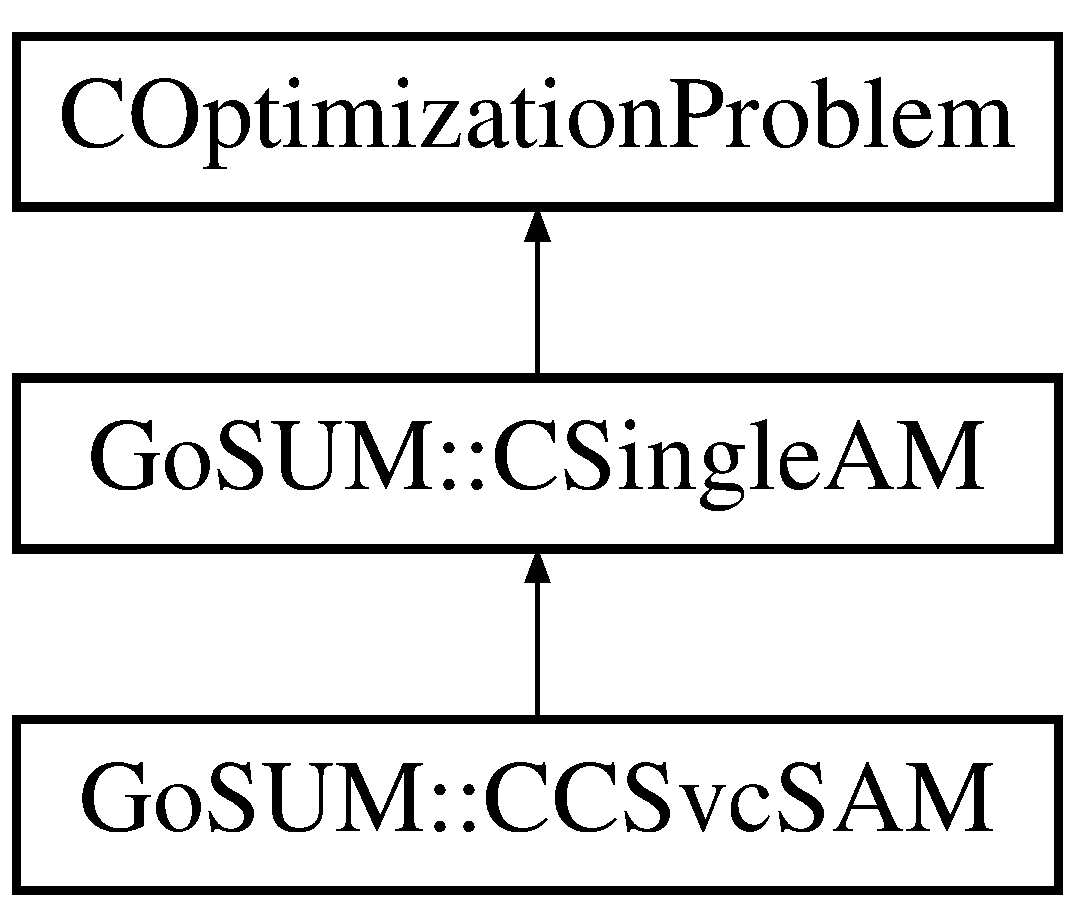
\includegraphics[height=3.000000cm]{class_go_s_u_m_1_1_c_c_svc_s_a_m}
\end{center}
\end{figure}
\subsection*{Public Member Functions}
\begin{DoxyCompactItemize}
\item 
\hyperlink{class_go_s_u_m_1_1_c_c_svc_s_a_m_acfee63e083350862a3a58f87508ecb3a}{C\-C\-Svc\-S\-A\-M} ()
\item 
virtual \hyperlink{class_go_s_u_m_1_1_c_c_svc_s_a_m_a5423b6bde13300396a2d19c08d1d9a28}{$\sim$\-C\-C\-Svc\-S\-A\-M} ()
\end{DoxyCompactItemize}
\subsection*{Protected Member Functions}
\begin{DoxyCompactItemize}
\item 
{\footnotesize template$<$class Archive $>$ }\\void \hyperlink{class_go_s_u_m_1_1_c_c_svc_s_a_m_ab6aa9113e26905e5606e86d5d23c1b03}{serialize} (Archive \&ar, const unsigned int version)
\end{DoxyCompactItemize}
\subsection*{Friends}
\begin{DoxyCompactItemize}
\item 
class \hyperlink{class_go_s_u_m_1_1_c_c_svc_s_a_m_ac98d07dd8f7b70e16ccb9a01abf56b9c}{boost\-::serialization\-::access}
\begin{DoxyCompactList}\small\item\em Boost serialization. \end{DoxyCompactList}\end{DoxyCompactItemize}
\subsection*{Additional Inherited Members}


\subsection{Detailed Description}
Class for the analyitical model for single output state, S\-V\-C type. 

\subsection{Constructor \& Destructor Documentation}
\hypertarget{class_go_s_u_m_1_1_c_c_svc_s_a_m_acfee63e083350862a3a58f87508ecb3a}{\index{Go\-S\-U\-M\-::\-C\-C\-Svc\-S\-A\-M@{Go\-S\-U\-M\-::\-C\-C\-Svc\-S\-A\-M}!C\-C\-Svc\-S\-A\-M@{C\-C\-Svc\-S\-A\-M}}
\index{C\-C\-Svc\-S\-A\-M@{C\-C\-Svc\-S\-A\-M}!GoSUM::CCSvcSAM@{Go\-S\-U\-M\-::\-C\-C\-Svc\-S\-A\-M}}
\subsubsection[{C\-C\-Svc\-S\-A\-M}]{\setlength{\rightskip}{0pt plus 5cm}Go\-S\-U\-M\-::\-C\-C\-Svc\-S\-A\-M\-::\-C\-C\-Svc\-S\-A\-M (
\begin{DoxyParamCaption}
{}
\end{DoxyParamCaption}
)\hspace{0.3cm}{\ttfamily [inline]}}}\label{class_go_s_u_m_1_1_c_c_svc_s_a_m_acfee63e083350862a3a58f87508ecb3a}
\hypertarget{class_go_s_u_m_1_1_c_c_svc_s_a_m_a5423b6bde13300396a2d19c08d1d9a28}{\index{Go\-S\-U\-M\-::\-C\-C\-Svc\-S\-A\-M@{Go\-S\-U\-M\-::\-C\-C\-Svc\-S\-A\-M}!$\sim$\-C\-C\-Svc\-S\-A\-M@{$\sim$\-C\-C\-Svc\-S\-A\-M}}
\index{$\sim$\-C\-C\-Svc\-S\-A\-M@{$\sim$\-C\-C\-Svc\-S\-A\-M}!GoSUM::CCSvcSAM@{Go\-S\-U\-M\-::\-C\-C\-Svc\-S\-A\-M}}
\subsubsection[{$\sim$\-C\-C\-Svc\-S\-A\-M}]{\setlength{\rightskip}{0pt plus 5cm}virtual Go\-S\-U\-M\-::\-C\-C\-Svc\-S\-A\-M\-::$\sim$\-C\-C\-Svc\-S\-A\-M (
\begin{DoxyParamCaption}
{}
\end{DoxyParamCaption}
)\hspace{0.3cm}{\ttfamily [inline]}, {\ttfamily [virtual]}}}\label{class_go_s_u_m_1_1_c_c_svc_s_a_m_a5423b6bde13300396a2d19c08d1d9a28}


\subsection{Member Function Documentation}
\hypertarget{class_go_s_u_m_1_1_c_c_svc_s_a_m_ab6aa9113e26905e5606e86d5d23c1b03}{\index{Go\-S\-U\-M\-::\-C\-C\-Svc\-S\-A\-M@{Go\-S\-U\-M\-::\-C\-C\-Svc\-S\-A\-M}!serialize@{serialize}}
\index{serialize@{serialize}!GoSUM::CCSvcSAM@{Go\-S\-U\-M\-::\-C\-C\-Svc\-S\-A\-M}}
\subsubsection[{serialize}]{\setlength{\rightskip}{0pt plus 5cm}template$<$class Archive $>$ void Go\-S\-U\-M\-::\-C\-C\-Svc\-S\-A\-M\-::serialize (
\begin{DoxyParamCaption}
\item[{Archive \&}]{ar, }
\item[{const unsigned int}]{version}
\end{DoxyParamCaption}
)\hspace{0.3cm}{\ttfamily [protected]}}}\label{class_go_s_u_m_1_1_c_c_svc_s_a_m_ab6aa9113e26905e5606e86d5d23c1b03}


Reimplemented from \hyperlink{class_go_s_u_m_1_1_c_single_a_m_a761e514fefeb7324e5509571f1be3848}{Go\-S\-U\-M\-::\-C\-Single\-A\-M}.



\subsection{Friends And Related Function Documentation}
\hypertarget{class_go_s_u_m_1_1_c_c_svc_s_a_m_ac98d07dd8f7b70e16ccb9a01abf56b9c}{\index{Go\-S\-U\-M\-::\-C\-C\-Svc\-S\-A\-M@{Go\-S\-U\-M\-::\-C\-C\-Svc\-S\-A\-M}!boost\-::serialization\-::access@{boost\-::serialization\-::access}}
\index{boost\-::serialization\-::access@{boost\-::serialization\-::access}!GoSUM::CCSvcSAM@{Go\-S\-U\-M\-::\-C\-C\-Svc\-S\-A\-M}}
\subsubsection[{boost\-::serialization\-::access}]{\setlength{\rightskip}{0pt plus 5cm}friend class boost\-::serialization\-::access\hspace{0.3cm}{\ttfamily [friend]}}}\label{class_go_s_u_m_1_1_c_c_svc_s_a_m_ac98d07dd8f7b70e16ccb9a01abf56b9c}


Boost serialization. 



The documentation for this class was generated from the following files\-:\begin{DoxyCompactItemize}
\item 
C\-:/\-Development/core/\hyperlink{_analytical_model_8h}{Analytical\-Model.\-h}\item 
C\-:/\-Development/core/\hyperlink{_analytical_model_8cpp}{Analytical\-Model.\-cpp}\end{DoxyCompactItemize}

\hypertarget{class_go_s_u_m_1_1_c_c_voronoi_h_c}{\section{Go\-S\-U\-M\-:\-:C\-C\-Voronoi\-H\-C Class Reference}
\label{class_go_s_u_m_1_1_c_c_voronoi_h_c}\index{Go\-S\-U\-M\-::\-C\-C\-Voronoi\-H\-C@{Go\-S\-U\-M\-::\-C\-C\-Voronoi\-H\-C}}
}


{\ttfamily \#include $<$Hypercube.\-h$>$}

Inheritance diagram for Go\-S\-U\-M\-:\-:C\-C\-Voronoi\-H\-C\-:\begin{figure}[H]
\begin{center}
\leavevmode
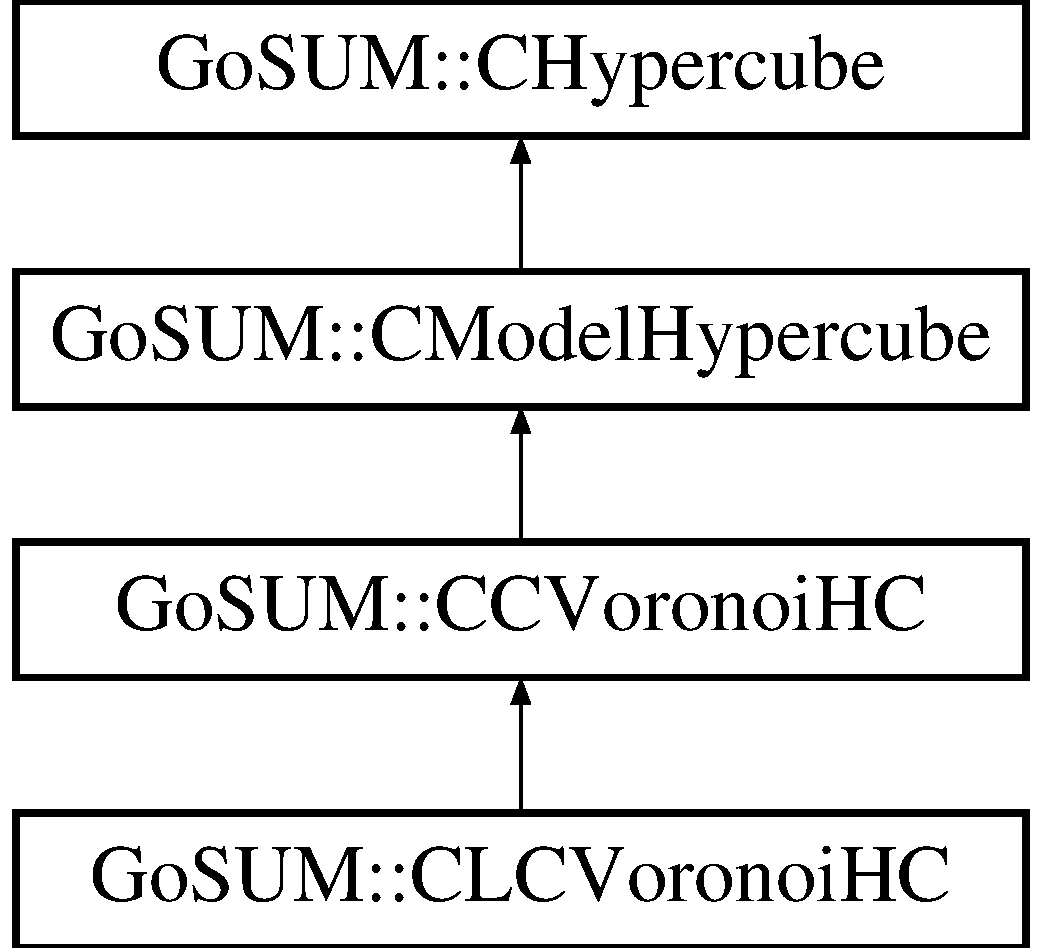
\includegraphics[height=4.000000cm]{class_go_s_u_m_1_1_c_c_voronoi_h_c}
\end{center}
\end{figure}
\subsection*{Public Member Functions}
\begin{DoxyCompactItemize}
\item 
\hyperlink{class_go_s_u_m_1_1_c_c_voronoi_h_c_ad3998fef79b2c64980c03fc2e3010c93}{C\-C\-Voronoi\-H\-C} (\hyperlink{class_go_s_u_m_1_1_c_input_parameters}{C\-Input\-Parameters} $\ast$\-\_\-p\-I\-P)
\item 
virtual \hyperlink{class_go_s_u_m_1_1_c_c_voronoi_h_c_afdcece721246023141339525c58256b6}{$\sim$\-C\-C\-Voronoi\-H\-C} ()
\end{DoxyCompactItemize}
\subsection*{Protected Member Functions}
\begin{DoxyCompactItemize}
\item 
{\footnotesize template$<$class Archive $>$ }\\void \hyperlink{class_go_s_u_m_1_1_c_c_voronoi_h_c_abbeaabd93028069b81be4dfc078e3d02}{serialize} (Archive \&ar, const unsigned int version)
\item 
virtual void \hyperlink{class_go_s_u_m_1_1_c_c_voronoi_h_c_ae3ecc9c8e8c09e42c13b77d0bfa8c020}{do\-Generate} (int \-\_\-rssize, int \-\_\-dim, std\-::vector$<$ Array\-Xd $>$ \&\-\_\-samples)
\begin{DoxyCompactList}\small\item\em Core of the generation. \end{DoxyCompactList}\item 
void \hyperlink{class_go_s_u_m_1_1_c_c_voronoi_h_c_a3988f3bc82cb71904e358ef13e9a68d4}{centralize} (std\-::vector$<$ Array\-Xd $>$ \&\-\_\-samples)
\begin{DoxyCompactList}\small\item\em Centralizes model points \-\_\-samples. \end{DoxyCompactList}\item 
\hyperlink{class_go_s_u_m_1_1_c_c_voronoi_h_c_a8c59858fea9d4e605b6207d8982b6931}{C\-C\-Voronoi\-H\-C} ()
\end{DoxyCompactItemize}
\subsection*{Friends}
\begin{DoxyCompactItemize}
\item 
class \hyperlink{class_go_s_u_m_1_1_c_c_voronoi_h_c_ac98d07dd8f7b70e16ccb9a01abf56b9c}{boost\-::serialization\-::access}
\begin{DoxyCompactList}\small\item\em Boost serialization. \end{DoxyCompactList}\end{DoxyCompactItemize}
\subsection*{Additional Inherited Members}


\subsection{Constructor \& Destructor Documentation}
\hypertarget{class_go_s_u_m_1_1_c_c_voronoi_h_c_a8c59858fea9d4e605b6207d8982b6931}{\index{Go\-S\-U\-M\-::\-C\-C\-Voronoi\-H\-C@{Go\-S\-U\-M\-::\-C\-C\-Voronoi\-H\-C}!C\-C\-Voronoi\-H\-C@{C\-C\-Voronoi\-H\-C}}
\index{C\-C\-Voronoi\-H\-C@{C\-C\-Voronoi\-H\-C}!GoSUM::CCVoronoiHC@{Go\-S\-U\-M\-::\-C\-C\-Voronoi\-H\-C}}
\subsubsection[{C\-C\-Voronoi\-H\-C}]{\setlength{\rightskip}{0pt plus 5cm}Go\-S\-U\-M\-::\-C\-C\-Voronoi\-H\-C\-::\-C\-C\-Voronoi\-H\-C (
\begin{DoxyParamCaption}
{}
\end{DoxyParamCaption}
)\hspace{0.3cm}{\ttfamily [inline]}, {\ttfamily [protected]}}}\label{class_go_s_u_m_1_1_c_c_voronoi_h_c_a8c59858fea9d4e605b6207d8982b6931}
\hypertarget{class_go_s_u_m_1_1_c_c_voronoi_h_c_ad3998fef79b2c64980c03fc2e3010c93}{\index{Go\-S\-U\-M\-::\-C\-C\-Voronoi\-H\-C@{Go\-S\-U\-M\-::\-C\-C\-Voronoi\-H\-C}!C\-C\-Voronoi\-H\-C@{C\-C\-Voronoi\-H\-C}}
\index{C\-C\-Voronoi\-H\-C@{C\-C\-Voronoi\-H\-C}!GoSUM::CCVoronoiHC@{Go\-S\-U\-M\-::\-C\-C\-Voronoi\-H\-C}}
\subsubsection[{C\-C\-Voronoi\-H\-C}]{\setlength{\rightskip}{0pt plus 5cm}Go\-S\-U\-M\-::\-C\-C\-Voronoi\-H\-C\-::\-C\-C\-Voronoi\-H\-C (
\begin{DoxyParamCaption}
\item[{{\bf C\-Input\-Parameters} $\ast$}]{\-\_\-p\-I\-P}
\end{DoxyParamCaption}
)\hspace{0.3cm}{\ttfamily [inline]}}}\label{class_go_s_u_m_1_1_c_c_voronoi_h_c_ad3998fef79b2c64980c03fc2e3010c93}
\hypertarget{class_go_s_u_m_1_1_c_c_voronoi_h_c_afdcece721246023141339525c58256b6}{\index{Go\-S\-U\-M\-::\-C\-C\-Voronoi\-H\-C@{Go\-S\-U\-M\-::\-C\-C\-Voronoi\-H\-C}!$\sim$\-C\-C\-Voronoi\-H\-C@{$\sim$\-C\-C\-Voronoi\-H\-C}}
\index{$\sim$\-C\-C\-Voronoi\-H\-C@{$\sim$\-C\-C\-Voronoi\-H\-C}!GoSUM::CCVoronoiHC@{Go\-S\-U\-M\-::\-C\-C\-Voronoi\-H\-C}}
\subsubsection[{$\sim$\-C\-C\-Voronoi\-H\-C}]{\setlength{\rightskip}{0pt plus 5cm}virtual Go\-S\-U\-M\-::\-C\-C\-Voronoi\-H\-C\-::$\sim$\-C\-C\-Voronoi\-H\-C (
\begin{DoxyParamCaption}
{}
\end{DoxyParamCaption}
)\hspace{0.3cm}{\ttfamily [inline]}, {\ttfamily [virtual]}}}\label{class_go_s_u_m_1_1_c_c_voronoi_h_c_afdcece721246023141339525c58256b6}


\subsection{Member Function Documentation}
\hypertarget{class_go_s_u_m_1_1_c_c_voronoi_h_c_a3988f3bc82cb71904e358ef13e9a68d4}{\index{Go\-S\-U\-M\-::\-C\-C\-Voronoi\-H\-C@{Go\-S\-U\-M\-::\-C\-C\-Voronoi\-H\-C}!centralize@{centralize}}
\index{centralize@{centralize}!GoSUM::CCVoronoiHC@{Go\-S\-U\-M\-::\-C\-C\-Voronoi\-H\-C}}
\subsubsection[{centralize}]{\setlength{\rightskip}{0pt plus 5cm}void Go\-S\-U\-M\-::\-C\-C\-Voronoi\-H\-C\-::centralize (
\begin{DoxyParamCaption}
\item[{std\-::vector$<$ Array\-Xd $>$ \&}]{\-\_\-samples}
\end{DoxyParamCaption}
)\hspace{0.3cm}{\ttfamily [protected]}}}\label{class_go_s_u_m_1_1_c_c_voronoi_h_c_a3988f3bc82cb71904e358ef13e9a68d4}


Centralizes model points \-\_\-samples. 

\hypertarget{class_go_s_u_m_1_1_c_c_voronoi_h_c_ae3ecc9c8e8c09e42c13b77d0bfa8c020}{\index{Go\-S\-U\-M\-::\-C\-C\-Voronoi\-H\-C@{Go\-S\-U\-M\-::\-C\-C\-Voronoi\-H\-C}!do\-Generate@{do\-Generate}}
\index{do\-Generate@{do\-Generate}!GoSUM::CCVoronoiHC@{Go\-S\-U\-M\-::\-C\-C\-Voronoi\-H\-C}}
\subsubsection[{do\-Generate}]{\setlength{\rightskip}{0pt plus 5cm}void Go\-S\-U\-M\-::\-C\-C\-Voronoi\-H\-C\-::do\-Generate (
\begin{DoxyParamCaption}
\item[{int}]{\-\_\-rssize, }
\item[{int}]{\-\_\-dim, }
\item[{std\-::vector$<$ Array\-Xd $>$ \&}]{\-\_\-samples}
\end{DoxyParamCaption}
)\hspace{0.3cm}{\ttfamily [protected]}, {\ttfamily [virtual]}}}\label{class_go_s_u_m_1_1_c_c_voronoi_h_c_ae3ecc9c8e8c09e42c13b77d0bfa8c020}


Core of the generation. 



Implements \hyperlink{class_go_s_u_m_1_1_c_model_hypercube_a1e92dd784f1c20b604fecd1a48bea2f4}{Go\-S\-U\-M\-::\-C\-Model\-Hypercube}.



Reimplemented in \hyperlink{class_go_s_u_m_1_1_c_l_c_voronoi_h_c_a02e90ea8deecafc3b398709f748fa9af}{Go\-S\-U\-M\-::\-C\-L\-C\-Voronoi\-H\-C}.

\hypertarget{class_go_s_u_m_1_1_c_c_voronoi_h_c_abbeaabd93028069b81be4dfc078e3d02}{\index{Go\-S\-U\-M\-::\-C\-C\-Voronoi\-H\-C@{Go\-S\-U\-M\-::\-C\-C\-Voronoi\-H\-C}!serialize@{serialize}}
\index{serialize@{serialize}!GoSUM::CCVoronoiHC@{Go\-S\-U\-M\-::\-C\-C\-Voronoi\-H\-C}}
\subsubsection[{serialize}]{\setlength{\rightskip}{0pt plus 5cm}template$<$class Archive $>$ void Go\-S\-U\-M\-::\-C\-C\-Voronoi\-H\-C\-::serialize (
\begin{DoxyParamCaption}
\item[{Archive \&}]{ar, }
\item[{const unsigned int}]{version}
\end{DoxyParamCaption}
)\hspace{0.3cm}{\ttfamily [protected]}}}\label{class_go_s_u_m_1_1_c_c_voronoi_h_c_abbeaabd93028069b81be4dfc078e3d02}


Reimplemented from \hyperlink{class_go_s_u_m_1_1_c_model_hypercube_a67de6632c6f6ca3685d2a750599974c6}{Go\-S\-U\-M\-::\-C\-Model\-Hypercube}.



Reimplemented in \hyperlink{class_go_s_u_m_1_1_c_l_c_voronoi_h_c_a98f588c33a8f2e2f4b681b48d63f2109}{Go\-S\-U\-M\-::\-C\-L\-C\-Voronoi\-H\-C}.



\subsection{Friends And Related Function Documentation}
\hypertarget{class_go_s_u_m_1_1_c_c_voronoi_h_c_ac98d07dd8f7b70e16ccb9a01abf56b9c}{\index{Go\-S\-U\-M\-::\-C\-C\-Voronoi\-H\-C@{Go\-S\-U\-M\-::\-C\-C\-Voronoi\-H\-C}!boost\-::serialization\-::access@{boost\-::serialization\-::access}}
\index{boost\-::serialization\-::access@{boost\-::serialization\-::access}!GoSUM::CCVoronoiHC@{Go\-S\-U\-M\-::\-C\-C\-Voronoi\-H\-C}}
\subsubsection[{boost\-::serialization\-::access}]{\setlength{\rightskip}{0pt plus 5cm}friend class boost\-::serialization\-::access\hspace{0.3cm}{\ttfamily [friend]}}}\label{class_go_s_u_m_1_1_c_c_voronoi_h_c_ac98d07dd8f7b70e16ccb9a01abf56b9c}


Boost serialization. 



The documentation for this class was generated from the following files\-:\begin{DoxyCompactItemize}
\item 
C\-:/\-Development/core/\hyperlink{_hypercube_8h}{Hypercube.\-h}\item 
C\-:/\-Development/core/\hyperlink{_hypercube_8cpp}{Hypercube.\-cpp}\end{DoxyCompactItemize}

\hypertarget{class_go_s_u_m_1_1_c_discrete_m_v}{\section{Go\-S\-U\-M\-:\-:C\-Discrete\-M\-V Class Reference}
\label{class_go_s_u_m_1_1_c_discrete_m_v}\index{Go\-S\-U\-M\-::\-C\-Discrete\-M\-V@{Go\-S\-U\-M\-::\-C\-Discrete\-M\-V}}
}


{\ttfamily \#include $<$Model\-Variable.\-h$>$}

Inheritance diagram for Go\-S\-U\-M\-:\-:C\-Discrete\-M\-V\-:\begin{figure}[H]
\begin{center}
\leavevmode
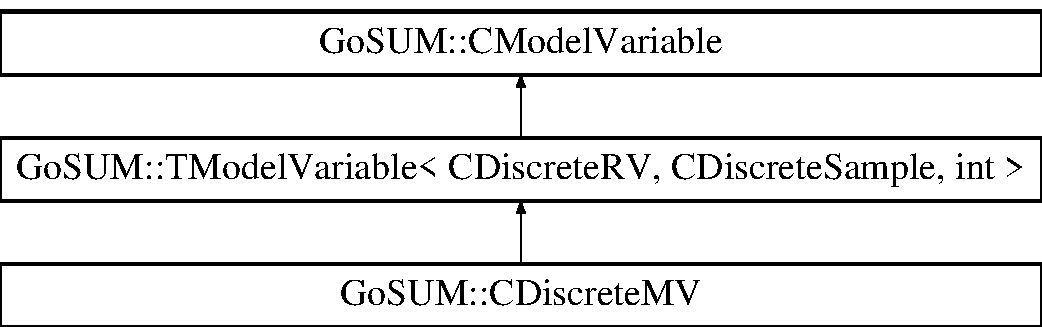
\includegraphics[height=3.000000cm]{class_go_s_u_m_1_1_c_discrete_m_v}
\end{center}
\end{figure}
\subsection*{Public Member Functions}
\begin{DoxyCompactItemize}
\item 
\hyperlink{class_go_s_u_m_1_1_c_discrete_m_v_aebbd9c3c4eae64d5ad99d8ea971d9c1e}{C\-Discrete\-M\-V} (const std\-::string \&\-\_\-uname, \hyperlink{class_c_random_variable_a80d2a87c43847274138b51f7d713d7f1}{C\-Random\-Variable\-::distributiontype} \-\_\-type)
\begin{DoxyCompactList}\small\item\em Constructs new model variable by name and type. \end{DoxyCompactList}\item 
\hyperlink{class_go_s_u_m_1_1_c_discrete_m_v_af7c40a5c6e0a54ae098e7c57e42ca64e}{C\-Discrete\-M\-V} (const \hyperlink{class_go_s_u_m_1_1_c_discrete_m_v}{C\-Discrete\-M\-V} \&O)
\item 
\hyperlink{class_go_s_u_m_1_1_c_discrete_m_v_a301a60a63864ffad50583b774e23b07b}{C\-Discrete\-M\-V} (const \hyperlink{class_go_s_u_m_1_1_c_continuous_m_v}{C\-Continuous\-M\-V} \&O)
\item 
virtual void \hyperlink{class_go_s_u_m_1_1_c_discrete_m_v_a1061fb0a466b852ffeb111238b702b39}{set\-Theoretical\-Distribution} ()
\begin{DoxyCompactList}\small\item\em Detects constant sample and turns random variable to appropirate type. \end{DoxyCompactList}\item 
virtual void \hyperlink{class_go_s_u_m_1_1_c_discrete_m_v_a7dd5ab7ac4922cdb2682012c942e1f10}{set\-Empirical\-Distribution} ()
\begin{DoxyCompactList}\small\item\em Compute distribution of the actual random variable from empirical sample data. \end{DoxyCompactList}\item 
virtual bool \hyperlink{class_go_s_u_m_1_1_c_discrete_m_v_a6366f6f6fd00242942b733ef5715592e}{is\-Continuous} () const 
\begin{DoxyCompactList}\small\item\em Returns true if model variable is continuous, false otherwise. \end{DoxyCompactList}\item 
virtual bool \hyperlink{class_go_s_u_m_1_1_c_discrete_m_v_ad9da78f518019e7133440189803f9cad}{is\-Discrete} () const 
\begin{DoxyCompactList}\small\item\em Returns true if model variable is discrete, false otherwise. \end{DoxyCompactList}\end{DoxyCompactItemize}
\subsection*{Private Member Functions}
\begin{DoxyCompactItemize}
\item 
{\footnotesize template$<$class Archive $>$ }\\void \hyperlink{class_go_s_u_m_1_1_c_discrete_m_v_a951630f04eefaf3e1604d801a75c2cc5}{serialize} (Archive \&ar, const unsigned int version)
\item 
\hyperlink{class_go_s_u_m_1_1_c_discrete_m_v_a2e384c7bd6c78c1cb2e8d5f3edf89151}{C\-Discrete\-M\-V} ()
\end{DoxyCompactItemize}
\subsection*{Friends}
\begin{DoxyCompactItemize}
\item 
class \hyperlink{class_go_s_u_m_1_1_c_discrete_m_v_ac98d07dd8f7b70e16ccb9a01abf56b9c}{boost\-::serialization\-::access}
\begin{DoxyCompactList}\small\item\em Boost serialization. \end{DoxyCompactList}\end{DoxyCompactItemize}
\subsection*{Additional Inherited Members}


\subsection{Constructor \& Destructor Documentation}
\hypertarget{class_go_s_u_m_1_1_c_discrete_m_v_a2e384c7bd6c78c1cb2e8d5f3edf89151}{\index{Go\-S\-U\-M\-::\-C\-Discrete\-M\-V@{Go\-S\-U\-M\-::\-C\-Discrete\-M\-V}!C\-Discrete\-M\-V@{C\-Discrete\-M\-V}}
\index{C\-Discrete\-M\-V@{C\-Discrete\-M\-V}!GoSUM::CDiscreteMV@{Go\-S\-U\-M\-::\-C\-Discrete\-M\-V}}
\subsubsection[{C\-Discrete\-M\-V}]{\setlength{\rightskip}{0pt plus 5cm}Go\-S\-U\-M\-::\-C\-Discrete\-M\-V\-::\-C\-Discrete\-M\-V (
\begin{DoxyParamCaption}
{}
\end{DoxyParamCaption}
)\hspace{0.3cm}{\ttfamily [inline]}, {\ttfamily [private]}}}\label{class_go_s_u_m_1_1_c_discrete_m_v_a2e384c7bd6c78c1cb2e8d5f3edf89151}
\hypertarget{class_go_s_u_m_1_1_c_discrete_m_v_aebbd9c3c4eae64d5ad99d8ea971d9c1e}{\index{Go\-S\-U\-M\-::\-C\-Discrete\-M\-V@{Go\-S\-U\-M\-::\-C\-Discrete\-M\-V}!C\-Discrete\-M\-V@{C\-Discrete\-M\-V}}
\index{C\-Discrete\-M\-V@{C\-Discrete\-M\-V}!GoSUM::CDiscreteMV@{Go\-S\-U\-M\-::\-C\-Discrete\-M\-V}}
\subsubsection[{C\-Discrete\-M\-V}]{\setlength{\rightskip}{0pt plus 5cm}Go\-S\-U\-M\-::\-C\-Discrete\-M\-V\-::\-C\-Discrete\-M\-V (
\begin{DoxyParamCaption}
\item[{const std\-::string \&}]{\-\_\-uname, }
\item[{{\bf C\-Random\-Variable\-::distributiontype}}]{\-\_\-type}
\end{DoxyParamCaption}
)}}\label{class_go_s_u_m_1_1_c_discrete_m_v_aebbd9c3c4eae64d5ad99d8ea971d9c1e}


Constructs new model variable by name and type. 

\hypertarget{class_go_s_u_m_1_1_c_discrete_m_v_af7c40a5c6e0a54ae098e7c57e42ca64e}{\index{Go\-S\-U\-M\-::\-C\-Discrete\-M\-V@{Go\-S\-U\-M\-::\-C\-Discrete\-M\-V}!C\-Discrete\-M\-V@{C\-Discrete\-M\-V}}
\index{C\-Discrete\-M\-V@{C\-Discrete\-M\-V}!GoSUM::CDiscreteMV@{Go\-S\-U\-M\-::\-C\-Discrete\-M\-V}}
\subsubsection[{C\-Discrete\-M\-V}]{\setlength{\rightskip}{0pt plus 5cm}Go\-S\-U\-M\-::\-C\-Discrete\-M\-V\-::\-C\-Discrete\-M\-V (
\begin{DoxyParamCaption}
\item[{const {\bf C\-Discrete\-M\-V} \&}]{O}
\end{DoxyParamCaption}
)}}\label{class_go_s_u_m_1_1_c_discrete_m_v_af7c40a5c6e0a54ae098e7c57e42ca64e}
\hypertarget{class_go_s_u_m_1_1_c_discrete_m_v_a301a60a63864ffad50583b774e23b07b}{\index{Go\-S\-U\-M\-::\-C\-Discrete\-M\-V@{Go\-S\-U\-M\-::\-C\-Discrete\-M\-V}!C\-Discrete\-M\-V@{C\-Discrete\-M\-V}}
\index{C\-Discrete\-M\-V@{C\-Discrete\-M\-V}!GoSUM::CDiscreteMV@{Go\-S\-U\-M\-::\-C\-Discrete\-M\-V}}
\subsubsection[{C\-Discrete\-M\-V}]{\setlength{\rightskip}{0pt plus 5cm}Go\-S\-U\-M\-::\-C\-Discrete\-M\-V\-::\-C\-Discrete\-M\-V (
\begin{DoxyParamCaption}
\item[{const {\bf C\-Continuous\-M\-V} \&}]{O}
\end{DoxyParamCaption}
)}}\label{class_go_s_u_m_1_1_c_discrete_m_v_a301a60a63864ffad50583b774e23b07b}


\subsection{Member Function Documentation}
\hypertarget{class_go_s_u_m_1_1_c_discrete_m_v_a6366f6f6fd00242942b733ef5715592e}{\index{Go\-S\-U\-M\-::\-C\-Discrete\-M\-V@{Go\-S\-U\-M\-::\-C\-Discrete\-M\-V}!is\-Continuous@{is\-Continuous}}
\index{is\-Continuous@{is\-Continuous}!GoSUM::CDiscreteMV@{Go\-S\-U\-M\-::\-C\-Discrete\-M\-V}}
\subsubsection[{is\-Continuous}]{\setlength{\rightskip}{0pt plus 5cm}virtual bool Go\-S\-U\-M\-::\-C\-Discrete\-M\-V\-::is\-Continuous (
\begin{DoxyParamCaption}
{}
\end{DoxyParamCaption}
) const\hspace{0.3cm}{\ttfamily [inline]}, {\ttfamily [virtual]}}}\label{class_go_s_u_m_1_1_c_discrete_m_v_a6366f6f6fd00242942b733ef5715592e}


Returns true if model variable is continuous, false otherwise. 



Implements \hyperlink{class_go_s_u_m_1_1_c_model_variable_a2ec4aee717249dcbad98fd6e6320a6b7}{Go\-S\-U\-M\-::\-C\-Model\-Variable}.

\hypertarget{class_go_s_u_m_1_1_c_discrete_m_v_ad9da78f518019e7133440189803f9cad}{\index{Go\-S\-U\-M\-::\-C\-Discrete\-M\-V@{Go\-S\-U\-M\-::\-C\-Discrete\-M\-V}!is\-Discrete@{is\-Discrete}}
\index{is\-Discrete@{is\-Discrete}!GoSUM::CDiscreteMV@{Go\-S\-U\-M\-::\-C\-Discrete\-M\-V}}
\subsubsection[{is\-Discrete}]{\setlength{\rightskip}{0pt plus 5cm}virtual bool Go\-S\-U\-M\-::\-C\-Discrete\-M\-V\-::is\-Discrete (
\begin{DoxyParamCaption}
{}
\end{DoxyParamCaption}
) const\hspace{0.3cm}{\ttfamily [inline]}, {\ttfamily [virtual]}}}\label{class_go_s_u_m_1_1_c_discrete_m_v_ad9da78f518019e7133440189803f9cad}


Returns true if model variable is discrete, false otherwise. 



Implements \hyperlink{class_go_s_u_m_1_1_c_model_variable_a9d0140b610b7a1c04a3b31e2d84f86da}{Go\-S\-U\-M\-::\-C\-Model\-Variable}.

\hypertarget{class_go_s_u_m_1_1_c_discrete_m_v_a951630f04eefaf3e1604d801a75c2cc5}{\index{Go\-S\-U\-M\-::\-C\-Discrete\-M\-V@{Go\-S\-U\-M\-::\-C\-Discrete\-M\-V}!serialize@{serialize}}
\index{serialize@{serialize}!GoSUM::CDiscreteMV@{Go\-S\-U\-M\-::\-C\-Discrete\-M\-V}}
\subsubsection[{serialize}]{\setlength{\rightskip}{0pt plus 5cm}template$<$class Archive $>$ void Go\-S\-U\-M\-::\-C\-Discrete\-M\-V\-::serialize (
\begin{DoxyParamCaption}
\item[{Archive \&}]{ar, }
\item[{const unsigned int}]{version}
\end{DoxyParamCaption}
)\hspace{0.3cm}{\ttfamily [inline]}, {\ttfamily [private]}}}\label{class_go_s_u_m_1_1_c_discrete_m_v_a951630f04eefaf3e1604d801a75c2cc5}
\hypertarget{class_go_s_u_m_1_1_c_discrete_m_v_a7dd5ab7ac4922cdb2682012c942e1f10}{\index{Go\-S\-U\-M\-::\-C\-Discrete\-M\-V@{Go\-S\-U\-M\-::\-C\-Discrete\-M\-V}!set\-Empirical\-Distribution@{set\-Empirical\-Distribution}}
\index{set\-Empirical\-Distribution@{set\-Empirical\-Distribution}!GoSUM::CDiscreteMV@{Go\-S\-U\-M\-::\-C\-Discrete\-M\-V}}
\subsubsection[{set\-Empirical\-Distribution}]{\setlength{\rightskip}{0pt plus 5cm}virtual void Go\-S\-U\-M\-::\-C\-Discrete\-M\-V\-::set\-Empirical\-Distribution (
\begin{DoxyParamCaption}
{}
\end{DoxyParamCaption}
)\hspace{0.3cm}{\ttfamily [inline]}, {\ttfamily [virtual]}}}\label{class_go_s_u_m_1_1_c_discrete_m_v_a7dd5ab7ac4922cdb2682012c942e1f10}


Compute distribution of the actual random variable from empirical sample data. 



Implements \hyperlink{class_go_s_u_m_1_1_t_model_variable_a3128d12e3ce0757714a7596de087314e}{Go\-S\-U\-M\-::\-T\-Model\-Variable$<$ R, S, t $>$}.

\hypertarget{class_go_s_u_m_1_1_c_discrete_m_v_a1061fb0a466b852ffeb111238b702b39}{\index{Go\-S\-U\-M\-::\-C\-Discrete\-M\-V@{Go\-S\-U\-M\-::\-C\-Discrete\-M\-V}!set\-Theoretical\-Distribution@{set\-Theoretical\-Distribution}}
\index{set\-Theoretical\-Distribution@{set\-Theoretical\-Distribution}!GoSUM::CDiscreteMV@{Go\-S\-U\-M\-::\-C\-Discrete\-M\-V}}
\subsubsection[{set\-Theoretical\-Distribution}]{\setlength{\rightskip}{0pt plus 5cm}void Go\-S\-U\-M\-::\-C\-Discrete\-M\-V\-::set\-Theoretical\-Distribution (
\begin{DoxyParamCaption}
{}
\end{DoxyParamCaption}
)\hspace{0.3cm}{\ttfamily [virtual]}}}\label{class_go_s_u_m_1_1_c_discrete_m_v_a1061fb0a466b852ffeb111238b702b39}


Detects constant sample and turns random variable to appropirate type. 



Implements \hyperlink{class_go_s_u_m_1_1_t_model_variable_ad113f33f216796f775855dd3f8553f03}{Go\-S\-U\-M\-::\-T\-Model\-Variable$<$ R, S, t $>$}.



\subsection{Friends And Related Function Documentation}
\hypertarget{class_go_s_u_m_1_1_c_discrete_m_v_ac98d07dd8f7b70e16ccb9a01abf56b9c}{\index{Go\-S\-U\-M\-::\-C\-Discrete\-M\-V@{Go\-S\-U\-M\-::\-C\-Discrete\-M\-V}!boost\-::serialization\-::access@{boost\-::serialization\-::access}}
\index{boost\-::serialization\-::access@{boost\-::serialization\-::access}!GoSUM::CDiscreteMV@{Go\-S\-U\-M\-::\-C\-Discrete\-M\-V}}
\subsubsection[{boost\-::serialization\-::access}]{\setlength{\rightskip}{0pt plus 5cm}friend class boost\-::serialization\-::access\hspace{0.3cm}{\ttfamily [friend]}}}\label{class_go_s_u_m_1_1_c_discrete_m_v_ac98d07dd8f7b70e16ccb9a01abf56b9c}


Boost serialization. 



The documentation for this class was generated from the following files\-:\begin{DoxyCompactItemize}
\item 
C\-:/\-Development/core/\hyperlink{_model_variable_8h}{Model\-Variable.\-h}\item 
C\-:/\-Development/core/\hyperlink{_model_variable_8cpp}{Model\-Variable.\-cpp}\end{DoxyCompactItemize}

\hypertarget{class_c_discrete_r_v}{\section{C\-Discrete\-R\-V Class Reference}
\label{class_c_discrete_r_v}\index{C\-Discrete\-R\-V@{C\-Discrete\-R\-V}}
}


{\ttfamily \#include $<$Random\-Variable.\-h$>$}

Inheritance diagram for C\-Discrete\-R\-V\-:\begin{figure}[H]
\begin{center}
\leavevmode
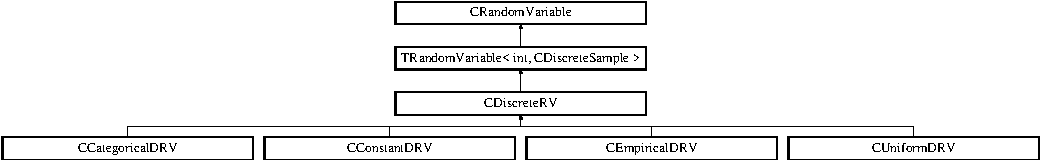
\includegraphics[height=2.129278cm]{class_c_discrete_r_v}
\end{center}
\end{figure}
\subsection*{Public Member Functions}
\begin{DoxyCompactItemize}
\item 
\hyperlink{class_c_discrete_r_v_a28c2505cde535e593d34362568b8853e}{C\-Discrete\-R\-V} ()
\item 
\hyperlink{class_c_discrete_r_v_a1da806969129ba38e8d7a03a3ee1ae34}{C\-Discrete\-R\-V} (const \hyperlink{class_c_discrete_r_v}{C\-Discrete\-R\-V} \&O)
\item 
virtual double \hyperlink{class_c_discrete_r_v_ab85fc494d5a2e900d5b135673e2bd750}{quantile} (double \-\_\-p) const 
\begin{DoxyCompactList}\small\item\em Quantile, only argument checking. \end{DoxyCompactList}\end{DoxyCompactItemize}
\subsection*{Private Member Functions}
\begin{DoxyCompactItemize}
\item 
{\footnotesize template$<$class Archive $>$ }\\void \hyperlink{class_c_discrete_r_v_a312904d56674cb277a94c3ad045cc4b8}{serialize} (Archive \&ar, const unsigned int version)
\end{DoxyCompactItemize}
\subsection*{Friends}
\begin{DoxyCompactItemize}
\item 
class \hyperlink{class_c_discrete_r_v_ac98d07dd8f7b70e16ccb9a01abf56b9c}{boost\-::serialization\-::access}
\begin{DoxyCompactList}\small\item\em Boost serialization. \end{DoxyCompactList}\end{DoxyCompactItemize}
\subsection*{Additional Inherited Members}


\subsection{Constructor \& Destructor Documentation}
\hypertarget{class_c_discrete_r_v_a28c2505cde535e593d34362568b8853e}{\index{C\-Discrete\-R\-V@{C\-Discrete\-R\-V}!C\-Discrete\-R\-V@{C\-Discrete\-R\-V}}
\index{C\-Discrete\-R\-V@{C\-Discrete\-R\-V}!CDiscreteRV@{C\-Discrete\-R\-V}}
\subsubsection[{C\-Discrete\-R\-V}]{\setlength{\rightskip}{0pt plus 5cm}C\-Discrete\-R\-V\-::\-C\-Discrete\-R\-V (
\begin{DoxyParamCaption}
{}
\end{DoxyParamCaption}
)\hspace{0.3cm}{\ttfamily [inline]}}}\label{class_c_discrete_r_v_a28c2505cde535e593d34362568b8853e}
\hypertarget{class_c_discrete_r_v_a1da806969129ba38e8d7a03a3ee1ae34}{\index{C\-Discrete\-R\-V@{C\-Discrete\-R\-V}!C\-Discrete\-R\-V@{C\-Discrete\-R\-V}}
\index{C\-Discrete\-R\-V@{C\-Discrete\-R\-V}!CDiscreteRV@{C\-Discrete\-R\-V}}
\subsubsection[{C\-Discrete\-R\-V}]{\setlength{\rightskip}{0pt plus 5cm}C\-Discrete\-R\-V\-::\-C\-Discrete\-R\-V (
\begin{DoxyParamCaption}
\item[{const {\bf C\-Discrete\-R\-V} \&}]{O}
\end{DoxyParamCaption}
)\hspace{0.3cm}{\ttfamily [inline]}}}\label{class_c_discrete_r_v_a1da806969129ba38e8d7a03a3ee1ae34}


\subsection{Member Function Documentation}
\hypertarget{class_c_discrete_r_v_ab85fc494d5a2e900d5b135673e2bd750}{\index{C\-Discrete\-R\-V@{C\-Discrete\-R\-V}!quantile@{quantile}}
\index{quantile@{quantile}!CDiscreteRV@{C\-Discrete\-R\-V}}
\subsubsection[{quantile}]{\setlength{\rightskip}{0pt plus 5cm}virtual double C\-Discrete\-R\-V\-::quantile (
\begin{DoxyParamCaption}
\item[{double}]{\-\_\-p}
\end{DoxyParamCaption}
) const\hspace{0.3cm}{\ttfamily [inline]}, {\ttfamily [virtual]}}}\label{class_c_discrete_r_v_ab85fc494d5a2e900d5b135673e2bd750}


Quantile, only argument checking. 



Implements \hyperlink{class_c_random_variable_aad8f00777fdad0e7e1ad29c9ea620ff2}{C\-Random\-Variable}.

\hypertarget{class_c_discrete_r_v_a312904d56674cb277a94c3ad045cc4b8}{\index{C\-Discrete\-R\-V@{C\-Discrete\-R\-V}!serialize@{serialize}}
\index{serialize@{serialize}!CDiscreteRV@{C\-Discrete\-R\-V}}
\subsubsection[{serialize}]{\setlength{\rightskip}{0pt plus 5cm}template$<$class Archive $>$ void C\-Discrete\-R\-V\-::serialize (
\begin{DoxyParamCaption}
\item[{Archive \&}]{ar, }
\item[{const unsigned int}]{version}
\end{DoxyParamCaption}
)\hspace{0.3cm}{\ttfamily [inline]}, {\ttfamily [private]}}}\label{class_c_discrete_r_v_a312904d56674cb277a94c3ad045cc4b8}


\subsection{Friends And Related Function Documentation}
\hypertarget{class_c_discrete_r_v_ac98d07dd8f7b70e16ccb9a01abf56b9c}{\index{C\-Discrete\-R\-V@{C\-Discrete\-R\-V}!boost\-::serialization\-::access@{boost\-::serialization\-::access}}
\index{boost\-::serialization\-::access@{boost\-::serialization\-::access}!CDiscreteRV@{C\-Discrete\-R\-V}}
\subsubsection[{boost\-::serialization\-::access}]{\setlength{\rightskip}{0pt plus 5cm}friend class boost\-::serialization\-::access\hspace{0.3cm}{\ttfamily [friend]}}}\label{class_c_discrete_r_v_ac98d07dd8f7b70e16ccb9a01abf56b9c}


Boost serialization. 



The documentation for this class was generated from the following file\-:\begin{DoxyCompactItemize}
\item 
C\-:/\-Development/core/\hyperlink{_random_variable_8h}{Random\-Variable.\-h}\end{DoxyCompactItemize}

\hypertarget{class_c_discrete_sample}{\section{C\-Discrete\-Sample Class Reference}
\label{class_c_discrete_sample}\index{C\-Discrete\-Sample@{C\-Discrete\-Sample}}
}


{\ttfamily \#include $<$Sample.\-h$>$}

Inheritance diagram for C\-Discrete\-Sample\-:\begin{figure}[H]
\begin{center}
\leavevmode
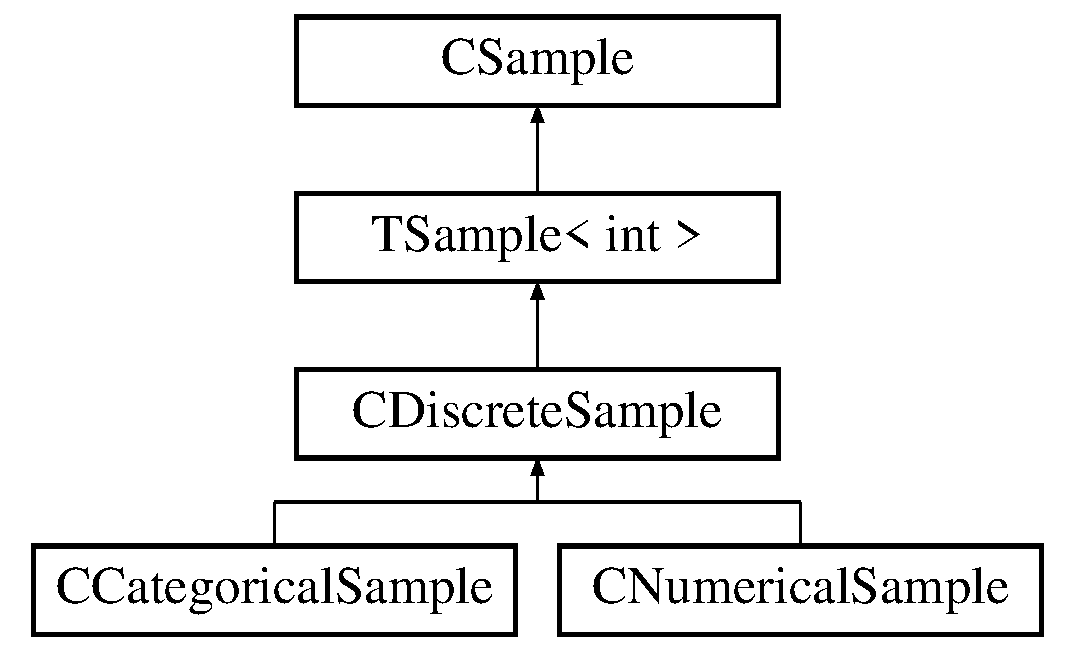
\includegraphics[height=4.000000cm]{class_c_discrete_sample}
\end{center}
\end{figure}
\subsection*{Public Member Functions}
\begin{DoxyCompactItemize}
\item 
\hyperlink{class_c_discrete_sample_ac891c831c15bb1dbbf5cabd94862893c}{C\-Discrete\-Sample} ()
\item 
virtual \hyperlink{class_c_discrete_sample_a5e3dbd761477945ac08a622409c9efdb}{$\sim$\-C\-Discrete\-Sample} ()
\item 
\hyperlink{class_c_discrete_sample_ab658862e3edd371c03a791bfb187eb4c}{C\-Discrete\-Sample} (const \hyperlink{class_c_discrete_sample}{C\-Discrete\-Sample} \&O)
\item 
virtual void \hyperlink{class_c_discrete_sample_a35f047c74401f8a3b83ec024579d049c}{compute\-Statistics} (int \-\_\-n)
\begin{DoxyCompactList}\small\item\em Computes sample statistics, i.\-e. normalized histogram etc. \end{DoxyCompactList}\item 
virtual int \hyperlink{class_c_discrete_sample_aca5d068b16f23c329d05af382ab68807}{export\-Histogram} (Array\-Xi \&\-\_\-x, Array\-Xd \&\-\_\-\-H) const 
\begin{DoxyCompactList}\small\item\em Exports histogram (x,H). \end{DoxyCompactList}\item 
virtual void \hyperlink{class_c_discrete_sample_a59a5822c0311f42f7fe3538ea729fd70}{export\-Sub\-Histogram} (Array\-Xd \&\-\_\-sub\-H, const std\-::vector$<$ int $>$ \&subset) const 
\begin{DoxyCompactList}\small\item\em Exports histogram relative to a subset of sample data. \end{DoxyCompactList}\item 
virtual double \hyperlink{class_c_discrete_sample_a3e2d5a72842be01a167f890960a34bef}{variance} () const 
\begin{DoxyCompactList}\small\item\em Returns sample variance (i.\-e.\-empirical). \end{DoxyCompactList}\end{DoxyCompactItemize}
\subsection*{Protected Member Functions}
\begin{DoxyCompactItemize}
\item 
{\footnotesize template$<$class Archive $>$ }\\void \hyperlink{class_c_discrete_sample_aa3e70fbd99f76fc47705c08d6230b726}{serialize} (Archive \&ar, const unsigned int version)
\end{DoxyCompactItemize}
\subsection*{Private Member Functions}
\begin{DoxyCompactItemize}
\item 
virtual void \hyperlink{class_c_discrete_sample_a3292af167095c8fc140dcb925e53fc58}{compute\-Normalized\-Histogram} (int \-\_\-n)
\begin{DoxyCompactList}\small\item\em C.\-omputes normalized histogram from sample data. \end{DoxyCompactList}\item 
virtual void \hyperlink{class_c_discrete_sample_a7056f6e7c8d98a88e272ef26dde01380}{compute\-Normalized\-Sub\-Histogram} (Array\-Xd \&\-\_\-sub\-H, const std\-::vector$<$ int $>$ \&subset) const 
\begin{DoxyCompactList}\small\item\em Computes normalized histogram from a subset of sample data. \end{DoxyCompactList}\end{DoxyCompactItemize}
\subsection*{Friends}
\begin{DoxyCompactItemize}
\item 
class \hyperlink{class_c_discrete_sample_ac98d07dd8f7b70e16ccb9a01abf56b9c}{boost\-::serialization\-::access}
\begin{DoxyCompactList}\small\item\em Boost serialization. \end{DoxyCompactList}\end{DoxyCompactItemize}
\subsection*{Additional Inherited Members}


\subsection{Constructor \& Destructor Documentation}
\hypertarget{class_c_discrete_sample_ac891c831c15bb1dbbf5cabd94862893c}{\index{C\-Discrete\-Sample@{C\-Discrete\-Sample}!C\-Discrete\-Sample@{C\-Discrete\-Sample}}
\index{C\-Discrete\-Sample@{C\-Discrete\-Sample}!CDiscreteSample@{C\-Discrete\-Sample}}
\subsubsection[{C\-Discrete\-Sample}]{\setlength{\rightskip}{0pt plus 5cm}C\-Discrete\-Sample\-::\-C\-Discrete\-Sample (
\begin{DoxyParamCaption}
{}
\end{DoxyParamCaption}
)\hspace{0.3cm}{\ttfamily [inline]}}}\label{class_c_discrete_sample_ac891c831c15bb1dbbf5cabd94862893c}
\hypertarget{class_c_discrete_sample_a5e3dbd761477945ac08a622409c9efdb}{\index{C\-Discrete\-Sample@{C\-Discrete\-Sample}!$\sim$\-C\-Discrete\-Sample@{$\sim$\-C\-Discrete\-Sample}}
\index{$\sim$\-C\-Discrete\-Sample@{$\sim$\-C\-Discrete\-Sample}!CDiscreteSample@{C\-Discrete\-Sample}}
\subsubsection[{$\sim$\-C\-Discrete\-Sample}]{\setlength{\rightskip}{0pt plus 5cm}virtual C\-Discrete\-Sample\-::$\sim$\-C\-Discrete\-Sample (
\begin{DoxyParamCaption}
{}
\end{DoxyParamCaption}
)\hspace{0.3cm}{\ttfamily [inline]}, {\ttfamily [virtual]}}}\label{class_c_discrete_sample_a5e3dbd761477945ac08a622409c9efdb}
\hypertarget{class_c_discrete_sample_ab658862e3edd371c03a791bfb187eb4c}{\index{C\-Discrete\-Sample@{C\-Discrete\-Sample}!C\-Discrete\-Sample@{C\-Discrete\-Sample}}
\index{C\-Discrete\-Sample@{C\-Discrete\-Sample}!CDiscreteSample@{C\-Discrete\-Sample}}
\subsubsection[{C\-Discrete\-Sample}]{\setlength{\rightskip}{0pt plus 5cm}C\-Discrete\-Sample\-::\-C\-Discrete\-Sample (
\begin{DoxyParamCaption}
\item[{const {\bf C\-Discrete\-Sample} \&}]{O}
\end{DoxyParamCaption}
)\hspace{0.3cm}{\ttfamily [inline]}}}\label{class_c_discrete_sample_ab658862e3edd371c03a791bfb187eb4c}


\subsection{Member Function Documentation}
\hypertarget{class_c_discrete_sample_a3292af167095c8fc140dcb925e53fc58}{\index{C\-Discrete\-Sample@{C\-Discrete\-Sample}!compute\-Normalized\-Histogram@{compute\-Normalized\-Histogram}}
\index{compute\-Normalized\-Histogram@{compute\-Normalized\-Histogram}!CDiscreteSample@{C\-Discrete\-Sample}}
\subsubsection[{compute\-Normalized\-Histogram}]{\setlength{\rightskip}{0pt plus 5cm}void C\-Discrete\-Sample\-::compute\-Normalized\-Histogram (
\begin{DoxyParamCaption}
\item[{int}]{\-\_\-n}
\end{DoxyParamCaption}
)\hspace{0.3cm}{\ttfamily [private]}, {\ttfamily [virtual]}}}\label{class_c_discrete_sample_a3292af167095c8fc140dcb925e53fc58}


C.\-omputes normalized histogram from sample data. 

\hypertarget{class_c_discrete_sample_a7056f6e7c8d98a88e272ef26dde01380}{\index{C\-Discrete\-Sample@{C\-Discrete\-Sample}!compute\-Normalized\-Sub\-Histogram@{compute\-Normalized\-Sub\-Histogram}}
\index{compute\-Normalized\-Sub\-Histogram@{compute\-Normalized\-Sub\-Histogram}!CDiscreteSample@{C\-Discrete\-Sample}}
\subsubsection[{compute\-Normalized\-Sub\-Histogram}]{\setlength{\rightskip}{0pt plus 5cm}void C\-Discrete\-Sample\-::compute\-Normalized\-Sub\-Histogram (
\begin{DoxyParamCaption}
\item[{Array\-Xd \&}]{\-\_\-sub\-H, }
\item[{const std\-::vector$<$ int $>$ \&}]{subset}
\end{DoxyParamCaption}
) const\hspace{0.3cm}{\ttfamily [private]}, {\ttfamily [virtual]}}}\label{class_c_discrete_sample_a7056f6e7c8d98a88e272ef26dde01380}


Computes normalized histogram from a subset of sample data. 

\hypertarget{class_c_discrete_sample_a35f047c74401f8a3b83ec024579d049c}{\index{C\-Discrete\-Sample@{C\-Discrete\-Sample}!compute\-Statistics@{compute\-Statistics}}
\index{compute\-Statistics@{compute\-Statistics}!CDiscreteSample@{C\-Discrete\-Sample}}
\subsubsection[{compute\-Statistics}]{\setlength{\rightskip}{0pt plus 5cm}virtual void C\-Discrete\-Sample\-::compute\-Statistics (
\begin{DoxyParamCaption}
\item[{int}]{\-\_\-n}
\end{DoxyParamCaption}
)\hspace{0.3cm}{\ttfamily [inline]}, {\ttfamily [virtual]}}}\label{class_c_discrete_sample_a35f047c74401f8a3b83ec024579d049c}


Computes sample statistics, i.\-e. normalized histogram etc. 



Implements \hyperlink{class_c_sample_a10000ec1dade335a2a96a8646e0bae03}{C\-Sample}.

\hypertarget{class_c_discrete_sample_aca5d068b16f23c329d05af382ab68807}{\index{C\-Discrete\-Sample@{C\-Discrete\-Sample}!export\-Histogram@{export\-Histogram}}
\index{export\-Histogram@{export\-Histogram}!CDiscreteSample@{C\-Discrete\-Sample}}
\subsubsection[{export\-Histogram}]{\setlength{\rightskip}{0pt plus 5cm}int C\-Discrete\-Sample\-::export\-Histogram (
\begin{DoxyParamCaption}
\item[{Array\-Xi \&}]{\-\_\-x, }
\item[{Array\-Xd \&}]{\-\_\-\-H}
\end{DoxyParamCaption}
) const\hspace{0.3cm}{\ttfamily [virtual]}}}\label{class_c_discrete_sample_aca5d068b16f23c329d05af382ab68807}


Exports histogram (x,H). 

\hypertarget{class_c_discrete_sample_a59a5822c0311f42f7fe3538ea729fd70}{\index{C\-Discrete\-Sample@{C\-Discrete\-Sample}!export\-Sub\-Histogram@{export\-Sub\-Histogram}}
\index{export\-Sub\-Histogram@{export\-Sub\-Histogram}!CDiscreteSample@{C\-Discrete\-Sample}}
\subsubsection[{export\-Sub\-Histogram}]{\setlength{\rightskip}{0pt plus 5cm}void C\-Discrete\-Sample\-::export\-Sub\-Histogram (
\begin{DoxyParamCaption}
\item[{Array\-Xd \&}]{\-\_\-sub\-H, }
\item[{const std\-::vector$<$ int $>$ \&}]{subset}
\end{DoxyParamCaption}
) const\hspace{0.3cm}{\ttfamily [virtual]}}}\label{class_c_discrete_sample_a59a5822c0311f42f7fe3538ea729fd70}


Exports histogram relative to a subset of sample data. 



Implements \hyperlink{class_t_sample_a1ce3bdd77627f5783edbec6f607c3ea9}{T\-Sample$<$ t $>$}.

\hypertarget{class_c_discrete_sample_aa3e70fbd99f76fc47705c08d6230b726}{\index{C\-Discrete\-Sample@{C\-Discrete\-Sample}!serialize@{serialize}}
\index{serialize@{serialize}!CDiscreteSample@{C\-Discrete\-Sample}}
\subsubsection[{serialize}]{\setlength{\rightskip}{0pt plus 5cm}template$<$class Archive $>$ void C\-Discrete\-Sample\-::serialize (
\begin{DoxyParamCaption}
\item[{Archive \&}]{ar, }
\item[{const unsigned int}]{version}
\end{DoxyParamCaption}
)\hspace{0.3cm}{\ttfamily [protected]}}}\label{class_c_discrete_sample_aa3e70fbd99f76fc47705c08d6230b726}


Reimplemented from \hyperlink{class_t_sample_a0f53b1db72dd3e83c50ab28dd31929a5}{T\-Sample$<$ t $>$}.

\hypertarget{class_c_discrete_sample_a3e2d5a72842be01a167f890960a34bef}{\index{C\-Discrete\-Sample@{C\-Discrete\-Sample}!variance@{variance}}
\index{variance@{variance}!CDiscreteSample@{C\-Discrete\-Sample}}
\subsubsection[{variance}]{\setlength{\rightskip}{0pt plus 5cm}virtual double C\-Discrete\-Sample\-::variance (
\begin{DoxyParamCaption}
{}
\end{DoxyParamCaption}
) const\hspace{0.3cm}{\ttfamily [inline]}, {\ttfamily [virtual]}}}\label{class_c_discrete_sample_a3e2d5a72842be01a167f890960a34bef}


Returns sample variance (i.\-e.\-empirical). 



Implements \hyperlink{class_c_sample_a5ce1e4ff44a8ac2e021dc36541343651}{C\-Sample}.



Reimplemented in \hyperlink{class_c_categorical_sample_a5408236fafb24d5a246823b97cc7427a}{C\-Categorical\-Sample}, and \hyperlink{class_c_numerical_sample_aedf72750cb229d9c17417ba787e487f1}{C\-Numerical\-Sample}.



\subsection{Friends And Related Function Documentation}
\hypertarget{class_c_discrete_sample_ac98d07dd8f7b70e16ccb9a01abf56b9c}{\index{C\-Discrete\-Sample@{C\-Discrete\-Sample}!boost\-::serialization\-::access@{boost\-::serialization\-::access}}
\index{boost\-::serialization\-::access@{boost\-::serialization\-::access}!CDiscreteSample@{C\-Discrete\-Sample}}
\subsubsection[{boost\-::serialization\-::access}]{\setlength{\rightskip}{0pt plus 5cm}friend class boost\-::serialization\-::access\hspace{0.3cm}{\ttfamily [friend]}}}\label{class_c_discrete_sample_ac98d07dd8f7b70e16ccb9a01abf56b9c}


Boost serialization. 



The documentation for this class was generated from the following files\-:\begin{DoxyCompactItemize}
\item 
C\-:/\-Development/core/\hyperlink{_sample_8h}{Sample.\-h}\item 
C\-:/\-Development/core/\hyperlink{_sample_8cpp}{Sample.\-cpp}\end{DoxyCompactItemize}

\hypertarget{class_go_s_u_m_1_1_c_d_sample_h_c}{\section{Go\-S\-U\-M\-:\-:C\-D\-Sample\-H\-C Class Reference}
\label{class_go_s_u_m_1_1_c_d_sample_h_c}\index{Go\-S\-U\-M\-::\-C\-D\-Sample\-H\-C@{Go\-S\-U\-M\-::\-C\-D\-Sample\-H\-C}}
}


{\ttfamily \#include $<$Hypercube.\-h$>$}

Inheritance diagram for Go\-S\-U\-M\-:\-:C\-D\-Sample\-H\-C\-:\begin{figure}[H]
\begin{center}
\leavevmode
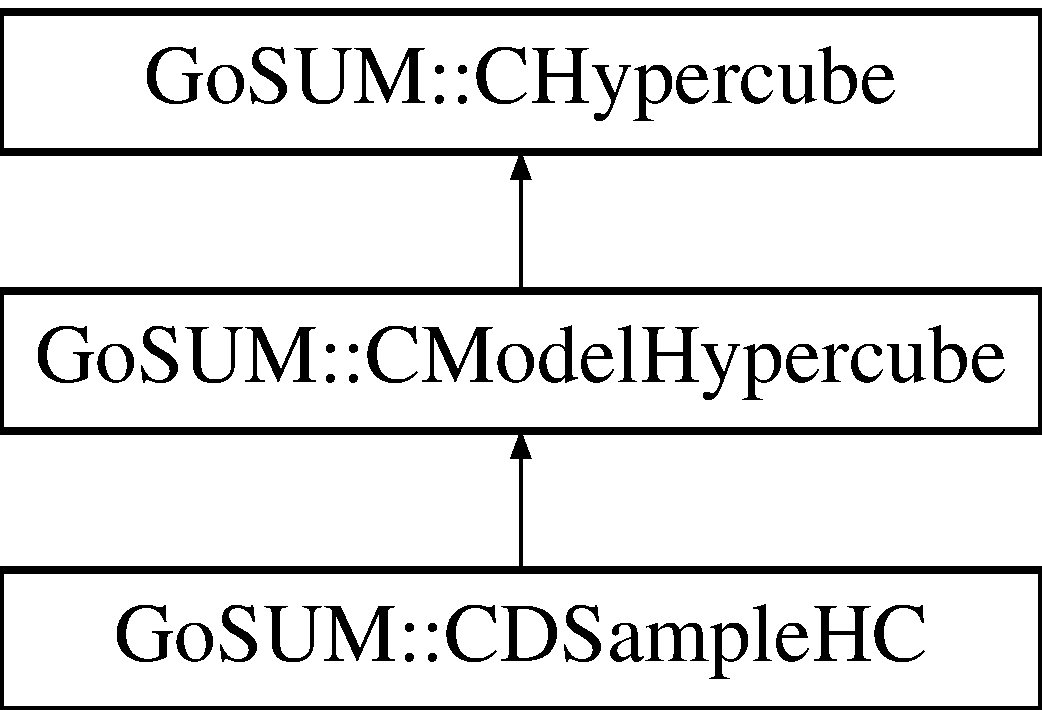
\includegraphics[height=3.000000cm]{class_go_s_u_m_1_1_c_d_sample_h_c}
\end{center}
\end{figure}
\subsection*{Public Member Functions}
\begin{DoxyCompactItemize}
\item 
\hyperlink{class_go_s_u_m_1_1_c_d_sample_h_c_a0140af8d61345c6108877a29b25e9e5d}{C\-D\-Sample\-H\-C} (\hyperlink{class_go_s_u_m_1_1_c_input_parameters}{C\-Input\-Parameters} $\ast$\-\_\-p\-I\-P)
\item 
virtual \hyperlink{class_go_s_u_m_1_1_c_d_sample_h_c_a423825a6ac94ef7707af0594077cefb3}{$\sim$\-C\-D\-Sample\-H\-C} ()
\end{DoxyCompactItemize}
\subsection*{Protected Member Functions}
\begin{DoxyCompactItemize}
\item 
virtual void \hyperlink{class_go_s_u_m_1_1_c_d_sample_h_c_aaa41eae7d120c7bf8d29ed2a0dc5c470}{do\-Generate} (int \-\_\-rssize, int \-\_\-dim, std\-::vector$<$ Array\-Xd $>$ \&\-\_\-samples)
\begin{DoxyCompactList}\small\item\em Core of the generation. \end{DoxyCompactList}\item 
\hyperlink{class_go_s_u_m_1_1_c_d_sample_h_c_a2c6787e78cca3e6f934c766f027d12c5}{C\-D\-Sample\-H\-C} ()
\end{DoxyCompactItemize}
\subsection*{Private Member Functions}
\begin{DoxyCompactItemize}
\item 
{\footnotesize template$<$class Archive $>$ }\\void \hyperlink{class_go_s_u_m_1_1_c_d_sample_h_c_a76df4a63843bc673d381c5410bc86c6d}{serialize} (Archive \&ar, const unsigned int version)
\end{DoxyCompactItemize}
\subsection*{Friends}
\begin{DoxyCompactItemize}
\item 
class \hyperlink{class_go_s_u_m_1_1_c_d_sample_h_c_ac98d07dd8f7b70e16ccb9a01abf56b9c}{boost\-::serialization\-::access}
\begin{DoxyCompactList}\small\item\em Boost serialization. \end{DoxyCompactList}\end{DoxyCompactItemize}
\subsection*{Additional Inherited Members}


\subsection{Constructor \& Destructor Documentation}
\hypertarget{class_go_s_u_m_1_1_c_d_sample_h_c_a2c6787e78cca3e6f934c766f027d12c5}{\index{Go\-S\-U\-M\-::\-C\-D\-Sample\-H\-C@{Go\-S\-U\-M\-::\-C\-D\-Sample\-H\-C}!C\-D\-Sample\-H\-C@{C\-D\-Sample\-H\-C}}
\index{C\-D\-Sample\-H\-C@{C\-D\-Sample\-H\-C}!GoSUM::CDSampleHC@{Go\-S\-U\-M\-::\-C\-D\-Sample\-H\-C}}
\subsubsection[{C\-D\-Sample\-H\-C}]{\setlength{\rightskip}{0pt plus 5cm}Go\-S\-U\-M\-::\-C\-D\-Sample\-H\-C\-::\-C\-D\-Sample\-H\-C (
\begin{DoxyParamCaption}
{}
\end{DoxyParamCaption}
)\hspace{0.3cm}{\ttfamily [inline]}, {\ttfamily [protected]}}}\label{class_go_s_u_m_1_1_c_d_sample_h_c_a2c6787e78cca3e6f934c766f027d12c5}
\hypertarget{class_go_s_u_m_1_1_c_d_sample_h_c_a0140af8d61345c6108877a29b25e9e5d}{\index{Go\-S\-U\-M\-::\-C\-D\-Sample\-H\-C@{Go\-S\-U\-M\-::\-C\-D\-Sample\-H\-C}!C\-D\-Sample\-H\-C@{C\-D\-Sample\-H\-C}}
\index{C\-D\-Sample\-H\-C@{C\-D\-Sample\-H\-C}!GoSUM::CDSampleHC@{Go\-S\-U\-M\-::\-C\-D\-Sample\-H\-C}}
\subsubsection[{C\-D\-Sample\-H\-C}]{\setlength{\rightskip}{0pt plus 5cm}Go\-S\-U\-M\-::\-C\-D\-Sample\-H\-C\-::\-C\-D\-Sample\-H\-C (
\begin{DoxyParamCaption}
\item[{{\bf C\-Input\-Parameters} $\ast$}]{\-\_\-p\-I\-P}
\end{DoxyParamCaption}
)\hspace{0.3cm}{\ttfamily [inline]}}}\label{class_go_s_u_m_1_1_c_d_sample_h_c_a0140af8d61345c6108877a29b25e9e5d}
\hypertarget{class_go_s_u_m_1_1_c_d_sample_h_c_a423825a6ac94ef7707af0594077cefb3}{\index{Go\-S\-U\-M\-::\-C\-D\-Sample\-H\-C@{Go\-S\-U\-M\-::\-C\-D\-Sample\-H\-C}!$\sim$\-C\-D\-Sample\-H\-C@{$\sim$\-C\-D\-Sample\-H\-C}}
\index{$\sim$\-C\-D\-Sample\-H\-C@{$\sim$\-C\-D\-Sample\-H\-C}!GoSUM::CDSampleHC@{Go\-S\-U\-M\-::\-C\-D\-Sample\-H\-C}}
\subsubsection[{$\sim$\-C\-D\-Sample\-H\-C}]{\setlength{\rightskip}{0pt plus 5cm}virtual Go\-S\-U\-M\-::\-C\-D\-Sample\-H\-C\-::$\sim$\-C\-D\-Sample\-H\-C (
\begin{DoxyParamCaption}
{}
\end{DoxyParamCaption}
)\hspace{0.3cm}{\ttfamily [inline]}, {\ttfamily [virtual]}}}\label{class_go_s_u_m_1_1_c_d_sample_h_c_a423825a6ac94ef7707af0594077cefb3}


\subsection{Member Function Documentation}
\hypertarget{class_go_s_u_m_1_1_c_d_sample_h_c_aaa41eae7d120c7bf8d29ed2a0dc5c470}{\index{Go\-S\-U\-M\-::\-C\-D\-Sample\-H\-C@{Go\-S\-U\-M\-::\-C\-D\-Sample\-H\-C}!do\-Generate@{do\-Generate}}
\index{do\-Generate@{do\-Generate}!GoSUM::CDSampleHC@{Go\-S\-U\-M\-::\-C\-D\-Sample\-H\-C}}
\subsubsection[{do\-Generate}]{\setlength{\rightskip}{0pt plus 5cm}void Go\-S\-U\-M\-::\-C\-D\-Sample\-H\-C\-::do\-Generate (
\begin{DoxyParamCaption}
\item[{int}]{\-\_\-rssize, }
\item[{int}]{\-\_\-dim, }
\item[{std\-::vector$<$ Array\-Xd $>$ \&}]{\-\_\-samples}
\end{DoxyParamCaption}
)\hspace{0.3cm}{\ttfamily [protected]}, {\ttfamily [virtual]}}}\label{class_go_s_u_m_1_1_c_d_sample_h_c_aaa41eae7d120c7bf8d29ed2a0dc5c470}


Core of the generation. 



Implements \hyperlink{class_go_s_u_m_1_1_c_model_hypercube_a1e92dd784f1c20b604fecd1a48bea2f4}{Go\-S\-U\-M\-::\-C\-Model\-Hypercube}.

\hypertarget{class_go_s_u_m_1_1_c_d_sample_h_c_a76df4a63843bc673d381c5410bc86c6d}{\index{Go\-S\-U\-M\-::\-C\-D\-Sample\-H\-C@{Go\-S\-U\-M\-::\-C\-D\-Sample\-H\-C}!serialize@{serialize}}
\index{serialize@{serialize}!GoSUM::CDSampleHC@{Go\-S\-U\-M\-::\-C\-D\-Sample\-H\-C}}
\subsubsection[{serialize}]{\setlength{\rightskip}{0pt plus 5cm}template$<$class Archive $>$ void Go\-S\-U\-M\-::\-C\-D\-Sample\-H\-C\-::serialize (
\begin{DoxyParamCaption}
\item[{Archive \&}]{ar, }
\item[{const unsigned int}]{version}
\end{DoxyParamCaption}
)\hspace{0.3cm}{\ttfamily [private]}}}\label{class_go_s_u_m_1_1_c_d_sample_h_c_a76df4a63843bc673d381c5410bc86c6d}


\subsection{Friends And Related Function Documentation}
\hypertarget{class_go_s_u_m_1_1_c_d_sample_h_c_ac98d07dd8f7b70e16ccb9a01abf56b9c}{\index{Go\-S\-U\-M\-::\-C\-D\-Sample\-H\-C@{Go\-S\-U\-M\-::\-C\-D\-Sample\-H\-C}!boost\-::serialization\-::access@{boost\-::serialization\-::access}}
\index{boost\-::serialization\-::access@{boost\-::serialization\-::access}!GoSUM::CDSampleHC@{Go\-S\-U\-M\-::\-C\-D\-Sample\-H\-C}}
\subsubsection[{boost\-::serialization\-::access}]{\setlength{\rightskip}{0pt plus 5cm}friend class boost\-::serialization\-::access\hspace{0.3cm}{\ttfamily [friend]}}}\label{class_go_s_u_m_1_1_c_d_sample_h_c_ac98d07dd8f7b70e16ccb9a01abf56b9c}


Boost serialization. 



The documentation for this class was generated from the following files\-:\begin{DoxyCompactItemize}
\item 
C\-:/\-Development/core/\hyperlink{_hypercube_8h}{Hypercube.\-h}\item 
C\-:/\-Development/core/\hyperlink{_hypercube_8cpp}{Hypercube.\-cpp}\end{DoxyCompactItemize}

\hypertarget{class_c_dynamic_system_r_n_g}{\section{C\-Dynamic\-System\-R\-N\-G Class Reference}
\label{class_c_dynamic_system_r_n_g}\index{C\-Dynamic\-System\-R\-N\-G@{C\-Dynamic\-System\-R\-N\-G}}
}


Class for dynamic system uniform R\-N\-G.  




{\ttfamily \#include $<$Random\-Generators.\-h$>$}

Inheritance diagram for C\-Dynamic\-System\-R\-N\-G\-:\begin{figure}[H]
\begin{center}
\leavevmode
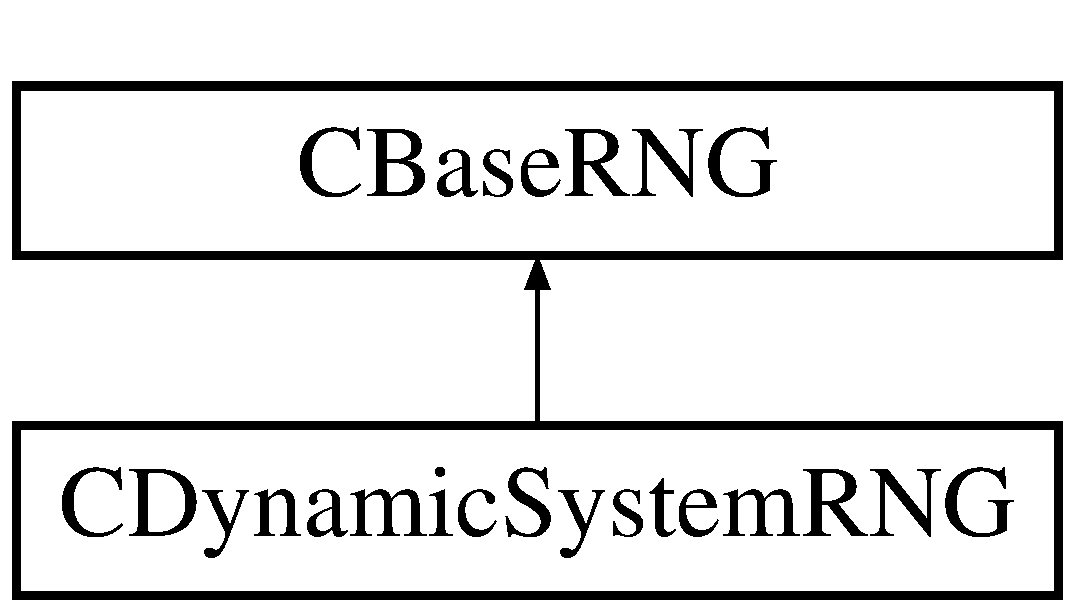
\includegraphics[height=2.000000cm]{class_c_dynamic_system_r_n_g}
\end{center}
\end{figure}
\subsection*{Public Member Functions}
\begin{DoxyCompactItemize}
\item 
\hyperlink{class_c_dynamic_system_r_n_g_af741112362509e7b12847b2d64d91d00}{C\-Dynamic\-System\-R\-N\-G} ()
\item 
\hyperlink{class_c_dynamic_system_r_n_g_a65373945f8ff6500313a43f866e60cd4}{C\-Dynamic\-System\-R\-N\-G} (unsigned int s)
\item 
virtual \hyperlink{class_c_dynamic_system_r_n_g_aa52982d8508d10e94de71e2f3c3f2ad5}{$\sim$\-C\-Dynamic\-System\-R\-N\-G} ()
\item 
virtual void \hyperlink{class_c_dynamic_system_r_n_g_a2ed468a45094e3c0591e0029b1359df1}{set\-Seed} (unsigned int s)
\begin{DoxyCompactList}\small\item\em Sets seed of the R\-N\-G. \end{DoxyCompactList}\item 
virtual unsigned int \hyperlink{class_c_dynamic_system_r_n_g_a703c33a722eb6808771245955e19b3e1}{rndi} ()
\begin{DoxyCompactList}\small\item\em Returns randomly generated unsigned int. \end{DoxyCompactList}\item 
virtual double \hyperlink{class_c_dynamic_system_r_n_g_af22e28ce058d489e0b73b08033db87b8}{rnd} ()
\begin{DoxyCompactList}\small\item\em Returns randomly generated double between 0 and 1. \end{DoxyCompactList}\end{DoxyCompactItemize}
\subsection*{Private Types}
\begin{DoxyCompactItemize}
\item 
typedef long long int \hyperlink{class_c_dynamic_system_r_n_g_ab5df6da5f9eaeb3d9cddc97405a09995}{Long}
\end{DoxyCompactItemize}
\subsection*{Private Member Functions}
\begin{DoxyCompactItemize}
\item 
Array$<$ long double, Dynamic, 1 $>$ \hyperlink{class_c_dynamic_system_r_n_g_abeca12f69df980c9bf34786d3acc850c}{prepare} (unsigned int M)
\begin{DoxyCompactList}\small\item\em Private function. \end{DoxyCompactList}\end{DoxyCompactItemize}
\subsection*{Private Attributes}
\begin{DoxyCompactItemize}
\item 
unsigned int \hyperlink{class_c_dynamic_system_r_n_g_ae8946db15d06d35b9080109bab84001c}{k}
\begin{DoxyCompactList}\small\item\em Paramters of the D\-S R\-N\-G. \end{DoxyCompactList}\item 
unsigned int \hyperlink{class_c_dynamic_system_r_n_g_a37d2707ee07015679697a2d9f1a2d4cd}{i}
\item 
unsigned int \hyperlink{class_c_dynamic_system_r_n_g_aec60b65b9e76642d7a36198e888d7e39}{j}
\begin{DoxyCompactList}\small\item\em Paramters of the D\-S R\-N\-G. \end{DoxyCompactList}\item 
\hyperlink{class_c_dynamic_system_r_n_g_ab5df6da5f9eaeb3d9cddc97405a09995}{Long} \hyperlink{class_c_dynamic_system_r_n_g_a8cdc452f933711c4146f9b6f8e9b53f2}{n}
\begin{DoxyCompactList}\small\item\em Paramters of the D\-S R\-N\-G. \end{DoxyCompactList}\item 
Array$<$ long double, Dynamic, 1 $>$ \hyperlink{class_c_dynamic_system_r_n_g_a41e389e017d88e1955ad45d237533560}{x}
\begin{DoxyCompactList}\small\item\em Paramters of the D\-S R\-N\-G. \end{DoxyCompactList}\item 
Array$<$ long double, Dynamic, 1 $>$ \hyperlink{class_c_dynamic_system_r_n_g_ad6d910566305fbb490cf785da19976e4}{w}
\begin{DoxyCompactList}\small\item\em Paramters of the D\-S R\-N\-G. \end{DoxyCompactList}\end{DoxyCompactItemize}


\subsection{Detailed Description}
Class for dynamic system uniform R\-N\-G. 

\subsection{Member Typedef Documentation}
\hypertarget{class_c_dynamic_system_r_n_g_ab5df6da5f9eaeb3d9cddc97405a09995}{\index{C\-Dynamic\-System\-R\-N\-G@{C\-Dynamic\-System\-R\-N\-G}!Long@{Long}}
\index{Long@{Long}!CDynamicSystemRNG@{C\-Dynamic\-System\-R\-N\-G}}
\subsubsection[{Long}]{\setlength{\rightskip}{0pt plus 5cm}typedef long long int {\bf C\-Dynamic\-System\-R\-N\-G\-::\-Long}\hspace{0.3cm}{\ttfamily [private]}}}\label{class_c_dynamic_system_r_n_g_ab5df6da5f9eaeb3d9cddc97405a09995}


\subsection{Constructor \& Destructor Documentation}
\hypertarget{class_c_dynamic_system_r_n_g_af741112362509e7b12847b2d64d91d00}{\index{C\-Dynamic\-System\-R\-N\-G@{C\-Dynamic\-System\-R\-N\-G}!C\-Dynamic\-System\-R\-N\-G@{C\-Dynamic\-System\-R\-N\-G}}
\index{C\-Dynamic\-System\-R\-N\-G@{C\-Dynamic\-System\-R\-N\-G}!CDynamicSystemRNG@{C\-Dynamic\-System\-R\-N\-G}}
\subsubsection[{C\-Dynamic\-System\-R\-N\-G}]{\setlength{\rightskip}{0pt plus 5cm}C\-Dynamic\-System\-R\-N\-G\-::\-C\-Dynamic\-System\-R\-N\-G (
\begin{DoxyParamCaption}
{}
\end{DoxyParamCaption}
)\hspace{0.3cm}{\ttfamily [inline]}}}\label{class_c_dynamic_system_r_n_g_af741112362509e7b12847b2d64d91d00}
\hypertarget{class_c_dynamic_system_r_n_g_a65373945f8ff6500313a43f866e60cd4}{\index{C\-Dynamic\-System\-R\-N\-G@{C\-Dynamic\-System\-R\-N\-G}!C\-Dynamic\-System\-R\-N\-G@{C\-Dynamic\-System\-R\-N\-G}}
\index{C\-Dynamic\-System\-R\-N\-G@{C\-Dynamic\-System\-R\-N\-G}!CDynamicSystemRNG@{C\-Dynamic\-System\-R\-N\-G}}
\subsubsection[{C\-Dynamic\-System\-R\-N\-G}]{\setlength{\rightskip}{0pt plus 5cm}C\-Dynamic\-System\-R\-N\-G\-::\-C\-Dynamic\-System\-R\-N\-G (
\begin{DoxyParamCaption}
\item[{unsigned int}]{s}
\end{DoxyParamCaption}
)\hspace{0.3cm}{\ttfamily [inline]}}}\label{class_c_dynamic_system_r_n_g_a65373945f8ff6500313a43f866e60cd4}
\hypertarget{class_c_dynamic_system_r_n_g_aa52982d8508d10e94de71e2f3c3f2ad5}{\index{C\-Dynamic\-System\-R\-N\-G@{C\-Dynamic\-System\-R\-N\-G}!$\sim$\-C\-Dynamic\-System\-R\-N\-G@{$\sim$\-C\-Dynamic\-System\-R\-N\-G}}
\index{$\sim$\-C\-Dynamic\-System\-R\-N\-G@{$\sim$\-C\-Dynamic\-System\-R\-N\-G}!CDynamicSystemRNG@{C\-Dynamic\-System\-R\-N\-G}}
\subsubsection[{$\sim$\-C\-Dynamic\-System\-R\-N\-G}]{\setlength{\rightskip}{0pt plus 5cm}virtual C\-Dynamic\-System\-R\-N\-G\-::$\sim$\-C\-Dynamic\-System\-R\-N\-G (
\begin{DoxyParamCaption}
{}
\end{DoxyParamCaption}
)\hspace{0.3cm}{\ttfamily [inline]}, {\ttfamily [virtual]}}}\label{class_c_dynamic_system_r_n_g_aa52982d8508d10e94de71e2f3c3f2ad5}


\subsection{Member Function Documentation}
\hypertarget{class_c_dynamic_system_r_n_g_abeca12f69df980c9bf34786d3acc850c}{\index{C\-Dynamic\-System\-R\-N\-G@{C\-Dynamic\-System\-R\-N\-G}!prepare@{prepare}}
\index{prepare@{prepare}!CDynamicSystemRNG@{C\-Dynamic\-System\-R\-N\-G}}
\subsubsection[{prepare}]{\setlength{\rightskip}{0pt plus 5cm}Array$<$ long double, Dynamic, 1 $>$ C\-Dynamic\-System\-R\-N\-G\-::prepare (
\begin{DoxyParamCaption}
\item[{unsigned int}]{M}
\end{DoxyParamCaption}
)\hspace{0.3cm}{\ttfamily [private]}}}\label{class_c_dynamic_system_r_n_g_abeca12f69df980c9bf34786d3acc850c}


Private function. 

\hypertarget{class_c_dynamic_system_r_n_g_af22e28ce058d489e0b73b08033db87b8}{\index{C\-Dynamic\-System\-R\-N\-G@{C\-Dynamic\-System\-R\-N\-G}!rnd@{rnd}}
\index{rnd@{rnd}!CDynamicSystemRNG@{C\-Dynamic\-System\-R\-N\-G}}
\subsubsection[{rnd}]{\setlength{\rightskip}{0pt plus 5cm}virtual double C\-Dynamic\-System\-R\-N\-G\-::rnd (
\begin{DoxyParamCaption}
{}
\end{DoxyParamCaption}
)\hspace{0.3cm}{\ttfamily [inline]}, {\ttfamily [virtual]}}}\label{class_c_dynamic_system_r_n_g_af22e28ce058d489e0b73b08033db87b8}


Returns randomly generated double between 0 and 1. 



Implements \hyperlink{class_c_base_r_n_g_abbd60a5ecdc9502dd646434224ab5d6b}{C\-Base\-R\-N\-G}.

\hypertarget{class_c_dynamic_system_r_n_g_a703c33a722eb6808771245955e19b3e1}{\index{C\-Dynamic\-System\-R\-N\-G@{C\-Dynamic\-System\-R\-N\-G}!rndi@{rndi}}
\index{rndi@{rndi}!CDynamicSystemRNG@{C\-Dynamic\-System\-R\-N\-G}}
\subsubsection[{rndi}]{\setlength{\rightskip}{0pt plus 5cm}virtual unsigned int C\-Dynamic\-System\-R\-N\-G\-::rndi (
\begin{DoxyParamCaption}
{}
\end{DoxyParamCaption}
)\hspace{0.3cm}{\ttfamily [inline]}, {\ttfamily [virtual]}}}\label{class_c_dynamic_system_r_n_g_a703c33a722eb6808771245955e19b3e1}


Returns randomly generated unsigned int. 



Implements \hyperlink{class_c_base_r_n_g_a2db96fbf06a2f11b3613d422043fb7b8}{C\-Base\-R\-N\-G}.

\hypertarget{class_c_dynamic_system_r_n_g_a2ed468a45094e3c0591e0029b1359df1}{\index{C\-Dynamic\-System\-R\-N\-G@{C\-Dynamic\-System\-R\-N\-G}!set\-Seed@{set\-Seed}}
\index{set\-Seed@{set\-Seed}!CDynamicSystemRNG@{C\-Dynamic\-System\-R\-N\-G}}
\subsubsection[{set\-Seed}]{\setlength{\rightskip}{0pt plus 5cm}virtual void C\-Dynamic\-System\-R\-N\-G\-::set\-Seed (
\begin{DoxyParamCaption}
\item[{unsigned int}]{s}
\end{DoxyParamCaption}
)\hspace{0.3cm}{\ttfamily [inline]}, {\ttfamily [virtual]}}}\label{class_c_dynamic_system_r_n_g_a2ed468a45094e3c0591e0029b1359df1}


Sets seed of the R\-N\-G. 


\begin{DoxyParams}{Parameters}
{\em s} & Sets seed of the R\-N\-G. \\
\hline
\end{DoxyParams}


Implements \hyperlink{class_c_base_r_n_g_a56fbf75ca07b73954596ee04820e0b07}{C\-Base\-R\-N\-G}.



\subsection{Member Data Documentation}
\hypertarget{class_c_dynamic_system_r_n_g_a37d2707ee07015679697a2d9f1a2d4cd}{\index{C\-Dynamic\-System\-R\-N\-G@{C\-Dynamic\-System\-R\-N\-G}!i@{i}}
\index{i@{i}!CDynamicSystemRNG@{C\-Dynamic\-System\-R\-N\-G}}
\subsubsection[{i}]{\setlength{\rightskip}{0pt plus 5cm}unsigned int C\-Dynamic\-System\-R\-N\-G\-::i\hspace{0.3cm}{\ttfamily [private]}}}\label{class_c_dynamic_system_r_n_g_a37d2707ee07015679697a2d9f1a2d4cd}
\hypertarget{class_c_dynamic_system_r_n_g_aec60b65b9e76642d7a36198e888d7e39}{\index{C\-Dynamic\-System\-R\-N\-G@{C\-Dynamic\-System\-R\-N\-G}!j@{j}}
\index{j@{j}!CDynamicSystemRNG@{C\-Dynamic\-System\-R\-N\-G}}
\subsubsection[{j}]{\setlength{\rightskip}{0pt plus 5cm}unsigned int C\-Dynamic\-System\-R\-N\-G\-::j\hspace{0.3cm}{\ttfamily [private]}}}\label{class_c_dynamic_system_r_n_g_aec60b65b9e76642d7a36198e888d7e39}


Paramters of the D\-S R\-N\-G. 

\hypertarget{class_c_dynamic_system_r_n_g_ae8946db15d06d35b9080109bab84001c}{\index{C\-Dynamic\-System\-R\-N\-G@{C\-Dynamic\-System\-R\-N\-G}!k@{k}}
\index{k@{k}!CDynamicSystemRNG@{C\-Dynamic\-System\-R\-N\-G}}
\subsubsection[{k}]{\setlength{\rightskip}{0pt plus 5cm}unsigned int C\-Dynamic\-System\-R\-N\-G\-::k\hspace{0.3cm}{\ttfamily [private]}}}\label{class_c_dynamic_system_r_n_g_ae8946db15d06d35b9080109bab84001c}


Paramters of the D\-S R\-N\-G. 

\hypertarget{class_c_dynamic_system_r_n_g_a8cdc452f933711c4146f9b6f8e9b53f2}{\index{C\-Dynamic\-System\-R\-N\-G@{C\-Dynamic\-System\-R\-N\-G}!n@{n}}
\index{n@{n}!CDynamicSystemRNG@{C\-Dynamic\-System\-R\-N\-G}}
\subsubsection[{n}]{\setlength{\rightskip}{0pt plus 5cm}{\bf Long} C\-Dynamic\-System\-R\-N\-G\-::n\hspace{0.3cm}{\ttfamily [private]}}}\label{class_c_dynamic_system_r_n_g_a8cdc452f933711c4146f9b6f8e9b53f2}


Paramters of the D\-S R\-N\-G. 

\hypertarget{class_c_dynamic_system_r_n_g_ad6d910566305fbb490cf785da19976e4}{\index{C\-Dynamic\-System\-R\-N\-G@{C\-Dynamic\-System\-R\-N\-G}!w@{w}}
\index{w@{w}!CDynamicSystemRNG@{C\-Dynamic\-System\-R\-N\-G}}
\subsubsection[{w}]{\setlength{\rightskip}{0pt plus 5cm}Array$<$long double,Dynamic,1$>$ C\-Dynamic\-System\-R\-N\-G\-::w\hspace{0.3cm}{\ttfamily [private]}}}\label{class_c_dynamic_system_r_n_g_ad6d910566305fbb490cf785da19976e4}


Paramters of the D\-S R\-N\-G. 

\hypertarget{class_c_dynamic_system_r_n_g_a41e389e017d88e1955ad45d237533560}{\index{C\-Dynamic\-System\-R\-N\-G@{C\-Dynamic\-System\-R\-N\-G}!x@{x}}
\index{x@{x}!CDynamicSystemRNG@{C\-Dynamic\-System\-R\-N\-G}}
\subsubsection[{x}]{\setlength{\rightskip}{0pt plus 5cm}Array$<$long double,Dynamic,1$>$ C\-Dynamic\-System\-R\-N\-G\-::x\hspace{0.3cm}{\ttfamily [private]}}}\label{class_c_dynamic_system_r_n_g_a41e389e017d88e1955ad45d237533560}


Paramters of the D\-S R\-N\-G. 



The documentation for this class was generated from the following files\-:\begin{DoxyCompactItemize}
\item 
C\-:/\-Development/core/\hyperlink{_random_generators_8h}{Random\-Generators.\-h}\item 
C\-:/\-Development/core/\hyperlink{_random_generators_8cpp}{Random\-Generators.\-cpp}\end{DoxyCompactItemize}

\hypertarget{class_c_empirical_c_r_v}{\section{C\-Empirical\-C\-R\-V Class Reference}
\label{class_c_empirical_c_r_v}\index{C\-Empirical\-C\-R\-V@{C\-Empirical\-C\-R\-V}}
}


Class for empirical continuous random variables derived from continuous random variables.  




{\ttfamily \#include $<$Random\-Variable.\-h$>$}

Inheritance diagram for C\-Empirical\-C\-R\-V\-:\begin{figure}[H]
\begin{center}
\leavevmode
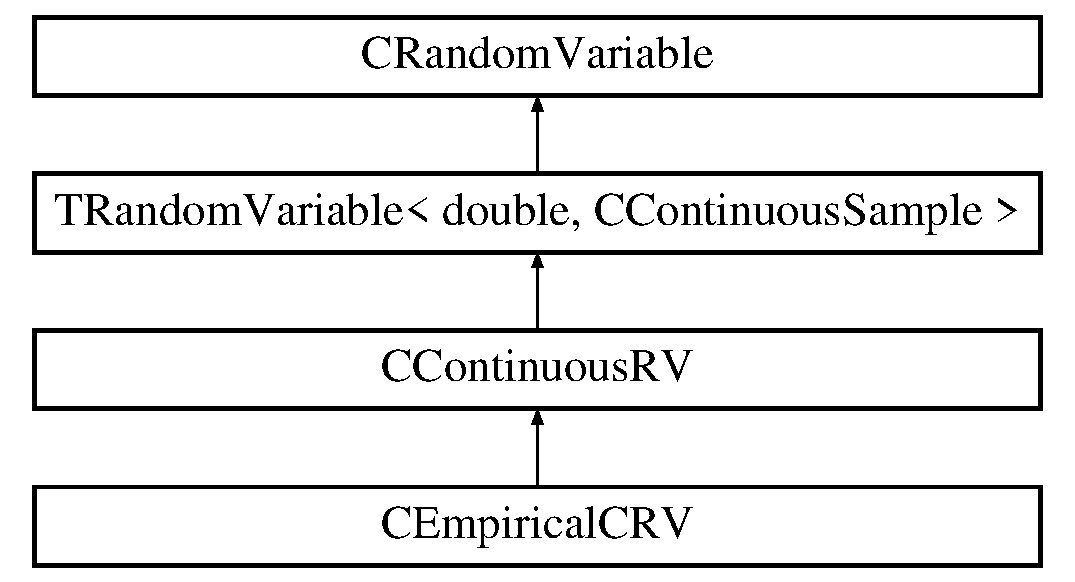
\includegraphics[height=4.000000cm]{class_c_empirical_c_r_v}
\end{center}
\end{figure}
\subsection*{Public Member Functions}
\begin{DoxyCompactItemize}
\item 
\hyperlink{class_c_empirical_c_r_v_a30962c974e7b95e126e82a25ead80e51}{C\-Empirical\-C\-R\-V} ()
\item 
virtual \hyperlink{class_c_empirical_c_r_v_a73ad37e7fa074113d13e3dbd8d6acf17}{$\sim$\-C\-Empirical\-C\-R\-V} ()
\item 
\hyperlink{class_c_empirical_c_r_v_acef0c749d1044e058a129e2326f39aa3}{C\-Empirical\-C\-R\-V} (const \hyperlink{class_c_empirical_c_r_v}{C\-Empirical\-C\-R\-V} \&O)
\item 
virtual void \hyperlink{class_c_empirical_c_r_v_a49362b1d3ad234fb978ec568199f16a6}{set\-Distribution} (const \hyperlink{class_c_continuous_sample}{C\-Continuous\-Sample} \&\-\_\-a\-S)
\begin{DoxyCompactList}\small\item\em Computes P\-M\-F and C\-D\-F from sample histogram, application of kernel densitiy estimation algorithm. \end{DoxyCompactList}\item 
virtual double \hyperlink{class_c_empirical_c_r_v_a2ada4c47c77c2028dd7d090baf6144c8}{probability} (double \-\_\-x) const 
\begin{DoxyCompactList}\small\item\em Function that returns P\-D\-F. \end{DoxyCompactList}\item 
virtual double \hyperlink{class_c_empirical_c_r_v_afd4ed84f573ef98c9be05ba96f5c02db}{cumulative} (double \-\_\-x) const 
\begin{DoxyCompactList}\small\item\em Function that returns C\-D\-F. \end{DoxyCompactList}\item 
virtual double \hyperlink{class_c_empirical_c_r_v_aa534b3d83beb19a6315eeee1d6810cc5}{min\-Value} () const 
\begin{DoxyCompactList}\small\item\em Returns minimal value of the random variable. \end{DoxyCompactList}\item 
virtual double \hyperlink{class_c_empirical_c_r_v_aaa748f04475940e62c12907e162e19b8}{max\-Value} () const 
\begin{DoxyCompactList}\small\item\em Eeturns maximal value of the random variable. \end{DoxyCompactList}\item 
virtual double \hyperlink{class_c_empirical_c_r_v_ab650ea825752fda0fe5d77790bda9d98}{expected\-Value} () const 
\begin{DoxyCompactList}\small\item\em Returns expected value of the random variable. \end{DoxyCompactList}\item 
virtual \hyperlink{class_c_random_variable_a80d2a87c43847274138b51f7d713d7f1}{distributiontype} \hyperlink{class_c_empirical_c_r_v_a3a05ff5a7dbceae66c3ec868f90a0c51}{distribution\-Type} () const 
\begin{DoxyCompactList}\small\item\em Returns enum type of the random variable distribution. \end{DoxyCompactList}\item 
virtual std\-::string \hyperlink{class_c_empirical_c_r_v_aa40d56ae3bdfafcd1ac595a4180bf33b}{distribution\-Name} () const 
\begin{DoxyCompactList}\small\item\em Returns name of the random variable distribution. \end{DoxyCompactList}\item 
virtual Array\-Xd \hyperlink{class_c_empirical_c_r_v_ae79ea609e95ae1cef28f7f6ec6e2cd73}{export\-Domain} () const 
\begin{DoxyCompactList}\small\item\em Exports domain of the random variable. \end{DoxyCompactList}\item 
virtual bool \hyperlink{class_c_empirical_c_r_v_a5a7d81a23bd1284497287440fbd2b160}{is\-Distribution\-Defined} () const 
\begin{DoxyCompactList}\small\item\em Returns true if distribution is defined, false otherwise. \end{DoxyCompactList}\item 
double \hyperlink{class_c_empirical_c_r_v_ac09b259e473b04aa40aa86e05b2a549c}{mean} () const 
\begin{DoxyCompactList}\small\item\em Returns mean of empirical random variable. \end{DoxyCompactList}\item 
double \hyperlink{class_c_empirical_c_r_v_a93d29fa2419b335adb1f099a35709b41}{standard\-Deviation} () const 
\begin{DoxyCompactList}\small\item\em Returns standard deviation of empirical random variable. \end{DoxyCompactList}\item 
virtual double \hyperlink{class_c_empirical_c_r_v_a0654170ccecffe3963db0c59c3d90d97}{variance} () const 
\begin{DoxyCompactList}\small\item\em Returns variance of the random variable. \end{DoxyCompactList}\end{DoxyCompactItemize}
\subsection*{Protected Member Functions}
\begin{DoxyCompactItemize}
\item 
virtual double \hyperlink{class_c_empirical_c_r_v_a86a5cc58d5aecb3c12f20d48c2d6c027}{do\-Quantile} (double \-\_\-p) const 
\begin{DoxyCompactList}\small\item\em Quantile, formula implementation. \end{DoxyCompactList}\end{DoxyCompactItemize}
\subsection*{Private Member Functions}
\begin{DoxyCompactItemize}
\item 
{\footnotesize template$<$class Archive $>$ }\\void \hyperlink{class_c_empirical_c_r_v_abb3f92128e9c135d612f2694d202b754}{serialize} (Archive \&ar, const unsigned int version)
\end{DoxyCompactItemize}
\subsection*{Private Attributes}
\begin{DoxyCompactItemize}
\item 
Array\-Xd \hyperlink{class_c_empirical_c_r_v_a9fa34c36e5695450ab958078517882ed}{x}
\item 
Array\-Xd \hyperlink{class_c_empirical_c_r_v_ab0e5305502410acb609ba60afa5e7de5}{p}
\item 
Array\-Xd \hyperlink{class_c_empirical_c_r_v_aab4138bc58b4031bf40d223b5444bc4d}{cdf}
\begin{DoxyCompactList}\small\item\em P\-D\-F (x,p) and C\-D\-F (x,cdf) data. \end{DoxyCompactList}\item 
double \hyperlink{class_c_empirical_c_r_v_aca50bd8bce019a6c82c2d1f65a1ec948}{pbandwidth}
\item 
double \hyperlink{class_c_empirical_c_r_v_a364ed1fc45edfa3a8569baa21de707d7}{qbandwidth}
\begin{DoxyCompactList}\small\item\em Bandwidths of P\-D\-F and C\-D\-F, as computed in kernel density estimator. \end{DoxyCompactList}\item 
double \hyperlink{class_c_empirical_c_r_v_a6fa15be69d72045664907de9f6c202ac}{mu}
\item 
double \hyperlink{class_c_empirical_c_r_v_aefa632e54ddee3239c56c55a0cbf748e}{stdv}
\end{DoxyCompactItemize}
\subsection*{Friends}
\begin{DoxyCompactItemize}
\item 
class \hyperlink{class_c_empirical_c_r_v_ac98d07dd8f7b70e16ccb9a01abf56b9c}{boost\-::serialization\-::access}
\begin{DoxyCompactList}\small\item\em Boost serialization. \end{DoxyCompactList}\end{DoxyCompactItemize}
\subsection*{Additional Inherited Members}


\subsection{Detailed Description}
Class for empirical continuous random variables derived from continuous random variables. 

\subsection{Constructor \& Destructor Documentation}
\hypertarget{class_c_empirical_c_r_v_a30962c974e7b95e126e82a25ead80e51}{\index{C\-Empirical\-C\-R\-V@{C\-Empirical\-C\-R\-V}!C\-Empirical\-C\-R\-V@{C\-Empirical\-C\-R\-V}}
\index{C\-Empirical\-C\-R\-V@{C\-Empirical\-C\-R\-V}!CEmpiricalCRV@{C\-Empirical\-C\-R\-V}}
\subsubsection[{C\-Empirical\-C\-R\-V}]{\setlength{\rightskip}{0pt plus 5cm}C\-Empirical\-C\-R\-V\-::\-C\-Empirical\-C\-R\-V (
\begin{DoxyParamCaption}
{}
\end{DoxyParamCaption}
)\hspace{0.3cm}{\ttfamily [inline]}}}\label{class_c_empirical_c_r_v_a30962c974e7b95e126e82a25ead80e51}
\hypertarget{class_c_empirical_c_r_v_a73ad37e7fa074113d13e3dbd8d6acf17}{\index{C\-Empirical\-C\-R\-V@{C\-Empirical\-C\-R\-V}!$\sim$\-C\-Empirical\-C\-R\-V@{$\sim$\-C\-Empirical\-C\-R\-V}}
\index{$\sim$\-C\-Empirical\-C\-R\-V@{$\sim$\-C\-Empirical\-C\-R\-V}!CEmpiricalCRV@{C\-Empirical\-C\-R\-V}}
\subsubsection[{$\sim$\-C\-Empirical\-C\-R\-V}]{\setlength{\rightskip}{0pt plus 5cm}virtual C\-Empirical\-C\-R\-V\-::$\sim$\-C\-Empirical\-C\-R\-V (
\begin{DoxyParamCaption}
{}
\end{DoxyParamCaption}
)\hspace{0.3cm}{\ttfamily [inline]}, {\ttfamily [virtual]}}}\label{class_c_empirical_c_r_v_a73ad37e7fa074113d13e3dbd8d6acf17}
\hypertarget{class_c_empirical_c_r_v_acef0c749d1044e058a129e2326f39aa3}{\index{C\-Empirical\-C\-R\-V@{C\-Empirical\-C\-R\-V}!C\-Empirical\-C\-R\-V@{C\-Empirical\-C\-R\-V}}
\index{C\-Empirical\-C\-R\-V@{C\-Empirical\-C\-R\-V}!CEmpiricalCRV@{C\-Empirical\-C\-R\-V}}
\subsubsection[{C\-Empirical\-C\-R\-V}]{\setlength{\rightskip}{0pt plus 5cm}C\-Empirical\-C\-R\-V\-::\-C\-Empirical\-C\-R\-V (
\begin{DoxyParamCaption}
\item[{const {\bf C\-Empirical\-C\-R\-V} \&}]{O}
\end{DoxyParamCaption}
)\hspace{0.3cm}{\ttfamily [inline]}}}\label{class_c_empirical_c_r_v_acef0c749d1044e058a129e2326f39aa3}


\subsection{Member Function Documentation}
\hypertarget{class_c_empirical_c_r_v_afd4ed84f573ef98c9be05ba96f5c02db}{\index{C\-Empirical\-C\-R\-V@{C\-Empirical\-C\-R\-V}!cumulative@{cumulative}}
\index{cumulative@{cumulative}!CEmpiricalCRV@{C\-Empirical\-C\-R\-V}}
\subsubsection[{cumulative}]{\setlength{\rightskip}{0pt plus 5cm}virtual double C\-Empirical\-C\-R\-V\-::cumulative (
\begin{DoxyParamCaption}
\item[{double}]{\-\_\-x}
\end{DoxyParamCaption}
) const\hspace{0.3cm}{\ttfamily [inline]}, {\ttfamily [virtual]}}}\label{class_c_empirical_c_r_v_afd4ed84f573ef98c9be05ba96f5c02db}


Function that returns C\-D\-F. 

\hypertarget{class_c_empirical_c_r_v_aa40d56ae3bdfafcd1ac595a4180bf33b}{\index{C\-Empirical\-C\-R\-V@{C\-Empirical\-C\-R\-V}!distribution\-Name@{distribution\-Name}}
\index{distribution\-Name@{distribution\-Name}!CEmpiricalCRV@{C\-Empirical\-C\-R\-V}}
\subsubsection[{distribution\-Name}]{\setlength{\rightskip}{0pt plus 5cm}virtual std\-::string C\-Empirical\-C\-R\-V\-::distribution\-Name (
\begin{DoxyParamCaption}
{}
\end{DoxyParamCaption}
) const\hspace{0.3cm}{\ttfamily [inline]}, {\ttfamily [virtual]}}}\label{class_c_empirical_c_r_v_aa40d56ae3bdfafcd1ac595a4180bf33b}


Returns name of the random variable distribution. 



Implements \hyperlink{class_c_random_variable_a4b33eef7c56f9f1a83af01fa8ef2502b}{C\-Random\-Variable}.

\hypertarget{class_c_empirical_c_r_v_a3a05ff5a7dbceae66c3ec868f90a0c51}{\index{C\-Empirical\-C\-R\-V@{C\-Empirical\-C\-R\-V}!distribution\-Type@{distribution\-Type}}
\index{distribution\-Type@{distribution\-Type}!CEmpiricalCRV@{C\-Empirical\-C\-R\-V}}
\subsubsection[{distribution\-Type}]{\setlength{\rightskip}{0pt plus 5cm}virtual {\bf distributiontype} C\-Empirical\-C\-R\-V\-::distribution\-Type (
\begin{DoxyParamCaption}
{}
\end{DoxyParamCaption}
) const\hspace{0.3cm}{\ttfamily [inline]}, {\ttfamily [virtual]}}}\label{class_c_empirical_c_r_v_a3a05ff5a7dbceae66c3ec868f90a0c51}


Returns enum type of the random variable distribution. 



Implements \hyperlink{class_c_random_variable_a3b30589d41f4dd200bd40c8273cac2cd}{C\-Random\-Variable}.

\hypertarget{class_c_empirical_c_r_v_a86a5cc58d5aecb3c12f20d48c2d6c027}{\index{C\-Empirical\-C\-R\-V@{C\-Empirical\-C\-R\-V}!do\-Quantile@{do\-Quantile}}
\index{do\-Quantile@{do\-Quantile}!CEmpiricalCRV@{C\-Empirical\-C\-R\-V}}
\subsubsection[{do\-Quantile}]{\setlength{\rightskip}{0pt plus 5cm}double C\-Empirical\-C\-R\-V\-::do\-Quantile (
\begin{DoxyParamCaption}
\item[{double}]{\-\_\-p}
\end{DoxyParamCaption}
) const\hspace{0.3cm}{\ttfamily [protected]}, {\ttfamily [virtual]}}}\label{class_c_empirical_c_r_v_a86a5cc58d5aecb3c12f20d48c2d6c027}


Quantile, formula implementation. 



Implements \hyperlink{class_c_random_variable_a552ab36c8144d7154cbe3cd363eee65b}{C\-Random\-Variable}.

\hypertarget{class_c_empirical_c_r_v_ab650ea825752fda0fe5d77790bda9d98}{\index{C\-Empirical\-C\-R\-V@{C\-Empirical\-C\-R\-V}!expected\-Value@{expected\-Value}}
\index{expected\-Value@{expected\-Value}!CEmpiricalCRV@{C\-Empirical\-C\-R\-V}}
\subsubsection[{expected\-Value}]{\setlength{\rightskip}{0pt plus 5cm}virtual double C\-Empirical\-C\-R\-V\-::expected\-Value (
\begin{DoxyParamCaption}
{}
\end{DoxyParamCaption}
) const\hspace{0.3cm}{\ttfamily [inline]}, {\ttfamily [virtual]}}}\label{class_c_empirical_c_r_v_ab650ea825752fda0fe5d77790bda9d98}


Returns expected value of the random variable. 



Implements \hyperlink{class_c_random_variable_a6e5490d17f2b6abcf9922c8b1bd6d4ed}{C\-Random\-Variable}.

\hypertarget{class_c_empirical_c_r_v_ae79ea609e95ae1cef28f7f6ec6e2cd73}{\index{C\-Empirical\-C\-R\-V@{C\-Empirical\-C\-R\-V}!export\-Domain@{export\-Domain}}
\index{export\-Domain@{export\-Domain}!CEmpiricalCRV@{C\-Empirical\-C\-R\-V}}
\subsubsection[{export\-Domain}]{\setlength{\rightskip}{0pt plus 5cm}Array\-Xd C\-Empirical\-C\-R\-V\-::export\-Domain (
\begin{DoxyParamCaption}
{}
\end{DoxyParamCaption}
) const\hspace{0.3cm}{\ttfamily [virtual]}}}\label{class_c_empirical_c_r_v_ae79ea609e95ae1cef28f7f6ec6e2cd73}


Exports domain of the random variable. 



Implements \hyperlink{class_t_random_variable_a37fc52d5fa37493a353887242d279a27}{T\-Random\-Variable$<$ t, T $>$}.

\hypertarget{class_c_empirical_c_r_v_a5a7d81a23bd1284497287440fbd2b160}{\index{C\-Empirical\-C\-R\-V@{C\-Empirical\-C\-R\-V}!is\-Distribution\-Defined@{is\-Distribution\-Defined}}
\index{is\-Distribution\-Defined@{is\-Distribution\-Defined}!CEmpiricalCRV@{C\-Empirical\-C\-R\-V}}
\subsubsection[{is\-Distribution\-Defined}]{\setlength{\rightskip}{0pt plus 5cm}virtual bool C\-Empirical\-C\-R\-V\-::is\-Distribution\-Defined (
\begin{DoxyParamCaption}
{}
\end{DoxyParamCaption}
) const\hspace{0.3cm}{\ttfamily [inline]}, {\ttfamily [virtual]}}}\label{class_c_empirical_c_r_v_a5a7d81a23bd1284497287440fbd2b160}


Returns true if distribution is defined, false otherwise. 



Reimplemented from \hyperlink{class_c_random_variable_a60e88c15450ab21dea6bef00d8836da7}{C\-Random\-Variable}.

\hypertarget{class_c_empirical_c_r_v_aaa748f04475940e62c12907e162e19b8}{\index{C\-Empirical\-C\-R\-V@{C\-Empirical\-C\-R\-V}!max\-Value@{max\-Value}}
\index{max\-Value@{max\-Value}!CEmpiricalCRV@{C\-Empirical\-C\-R\-V}}
\subsubsection[{max\-Value}]{\setlength{\rightskip}{0pt plus 5cm}virtual double C\-Empirical\-C\-R\-V\-::max\-Value (
\begin{DoxyParamCaption}
{}
\end{DoxyParamCaption}
) const\hspace{0.3cm}{\ttfamily [inline]}, {\ttfamily [virtual]}}}\label{class_c_empirical_c_r_v_aaa748f04475940e62c12907e162e19b8}


Eeturns maximal value of the random variable. 



Implements \hyperlink{class_c_random_variable_a48a5e98363d866f1f46568ed658479ad}{C\-Random\-Variable}.

\hypertarget{class_c_empirical_c_r_v_ac09b259e473b04aa40aa86e05b2a549c}{\index{C\-Empirical\-C\-R\-V@{C\-Empirical\-C\-R\-V}!mean@{mean}}
\index{mean@{mean}!CEmpiricalCRV@{C\-Empirical\-C\-R\-V}}
\subsubsection[{mean}]{\setlength{\rightskip}{0pt plus 5cm}double C\-Empirical\-C\-R\-V\-::mean (
\begin{DoxyParamCaption}
{}
\end{DoxyParamCaption}
) const\hspace{0.3cm}{\ttfamily [inline]}}}\label{class_c_empirical_c_r_v_ac09b259e473b04aa40aa86e05b2a549c}


Returns mean of empirical random variable. 

\hypertarget{class_c_empirical_c_r_v_aa534b3d83beb19a6315eeee1d6810cc5}{\index{C\-Empirical\-C\-R\-V@{C\-Empirical\-C\-R\-V}!min\-Value@{min\-Value}}
\index{min\-Value@{min\-Value}!CEmpiricalCRV@{C\-Empirical\-C\-R\-V}}
\subsubsection[{min\-Value}]{\setlength{\rightskip}{0pt plus 5cm}virtual double C\-Empirical\-C\-R\-V\-::min\-Value (
\begin{DoxyParamCaption}
{}
\end{DoxyParamCaption}
) const\hspace{0.3cm}{\ttfamily [inline]}, {\ttfamily [virtual]}}}\label{class_c_empirical_c_r_v_aa534b3d83beb19a6315eeee1d6810cc5}


Returns minimal value of the random variable. 



Implements \hyperlink{class_c_random_variable_a233ddd2eedb51b09a04a8c330646f356}{C\-Random\-Variable}.

\hypertarget{class_c_empirical_c_r_v_a2ada4c47c77c2028dd7d090baf6144c8}{\index{C\-Empirical\-C\-R\-V@{C\-Empirical\-C\-R\-V}!probability@{probability}}
\index{probability@{probability}!CEmpiricalCRV@{C\-Empirical\-C\-R\-V}}
\subsubsection[{probability}]{\setlength{\rightskip}{0pt plus 5cm}virtual double C\-Empirical\-C\-R\-V\-::probability (
\begin{DoxyParamCaption}
\item[{double}]{\-\_\-x}
\end{DoxyParamCaption}
) const\hspace{0.3cm}{\ttfamily [inline]}, {\ttfamily [virtual]}}}\label{class_c_empirical_c_r_v_a2ada4c47c77c2028dd7d090baf6144c8}


Function that returns P\-D\-F. 

\hypertarget{class_c_empirical_c_r_v_abb3f92128e9c135d612f2694d202b754}{\index{C\-Empirical\-C\-R\-V@{C\-Empirical\-C\-R\-V}!serialize@{serialize}}
\index{serialize@{serialize}!CEmpiricalCRV@{C\-Empirical\-C\-R\-V}}
\subsubsection[{serialize}]{\setlength{\rightskip}{0pt plus 5cm}template$<$class Archive $>$ void C\-Empirical\-C\-R\-V\-::serialize (
\begin{DoxyParamCaption}
\item[{Archive \&}]{ar, }
\item[{const unsigned int}]{version}
\end{DoxyParamCaption}
)\hspace{0.3cm}{\ttfamily [private]}}}\label{class_c_empirical_c_r_v_abb3f92128e9c135d612f2694d202b754}
\hypertarget{class_c_empirical_c_r_v_a49362b1d3ad234fb978ec568199f16a6}{\index{C\-Empirical\-C\-R\-V@{C\-Empirical\-C\-R\-V}!set\-Distribution@{set\-Distribution}}
\index{set\-Distribution@{set\-Distribution}!CEmpiricalCRV@{C\-Empirical\-C\-R\-V}}
\subsubsection[{set\-Distribution}]{\setlength{\rightskip}{0pt plus 5cm}void C\-Empirical\-C\-R\-V\-::set\-Distribution (
\begin{DoxyParamCaption}
\item[{const {\bf C\-Continuous\-Sample} \&}]{\-\_\-a\-S}
\end{DoxyParamCaption}
)\hspace{0.3cm}{\ttfamily [virtual]}}}\label{class_c_empirical_c_r_v_a49362b1d3ad234fb978ec568199f16a6}


Computes P\-M\-F and C\-D\-F from sample histogram, application of kernel densitiy estimation algorithm. 

\hypertarget{class_c_empirical_c_r_v_a93d29fa2419b335adb1f099a35709b41}{\index{C\-Empirical\-C\-R\-V@{C\-Empirical\-C\-R\-V}!standard\-Deviation@{standard\-Deviation}}
\index{standard\-Deviation@{standard\-Deviation}!CEmpiricalCRV@{C\-Empirical\-C\-R\-V}}
\subsubsection[{standard\-Deviation}]{\setlength{\rightskip}{0pt plus 5cm}double C\-Empirical\-C\-R\-V\-::standard\-Deviation (
\begin{DoxyParamCaption}
{}
\end{DoxyParamCaption}
) const\hspace{0.3cm}{\ttfamily [inline]}}}\label{class_c_empirical_c_r_v_a93d29fa2419b335adb1f099a35709b41}


Returns standard deviation of empirical random variable. 

\hypertarget{class_c_empirical_c_r_v_a0654170ccecffe3963db0c59c3d90d97}{\index{C\-Empirical\-C\-R\-V@{C\-Empirical\-C\-R\-V}!variance@{variance}}
\index{variance@{variance}!CEmpiricalCRV@{C\-Empirical\-C\-R\-V}}
\subsubsection[{variance}]{\setlength{\rightskip}{0pt plus 5cm}virtual double C\-Empirical\-C\-R\-V\-::variance (
\begin{DoxyParamCaption}
{}
\end{DoxyParamCaption}
) const\hspace{0.3cm}{\ttfamily [inline]}, {\ttfamily [virtual]}}}\label{class_c_empirical_c_r_v_a0654170ccecffe3963db0c59c3d90d97}


Returns variance of the random variable. 



Implements \hyperlink{class_c_random_variable_a3b0b87c4aab74c0406cd8321b8b96747}{C\-Random\-Variable}.



\subsection{Friends And Related Function Documentation}
\hypertarget{class_c_empirical_c_r_v_ac98d07dd8f7b70e16ccb9a01abf56b9c}{\index{C\-Empirical\-C\-R\-V@{C\-Empirical\-C\-R\-V}!boost\-::serialization\-::access@{boost\-::serialization\-::access}}
\index{boost\-::serialization\-::access@{boost\-::serialization\-::access}!CEmpiricalCRV@{C\-Empirical\-C\-R\-V}}
\subsubsection[{boost\-::serialization\-::access}]{\setlength{\rightskip}{0pt plus 5cm}friend class boost\-::serialization\-::access\hspace{0.3cm}{\ttfamily [friend]}}}\label{class_c_empirical_c_r_v_ac98d07dd8f7b70e16ccb9a01abf56b9c}


Boost serialization. 



\subsection{Member Data Documentation}
\hypertarget{class_c_empirical_c_r_v_aab4138bc58b4031bf40d223b5444bc4d}{\index{C\-Empirical\-C\-R\-V@{C\-Empirical\-C\-R\-V}!cdf@{cdf}}
\index{cdf@{cdf}!CEmpiricalCRV@{C\-Empirical\-C\-R\-V}}
\subsubsection[{cdf}]{\setlength{\rightskip}{0pt plus 5cm}Array\-Xd C\-Empirical\-C\-R\-V\-::cdf\hspace{0.3cm}{\ttfamily [private]}}}\label{class_c_empirical_c_r_v_aab4138bc58b4031bf40d223b5444bc4d}


P\-D\-F (x,p) and C\-D\-F (x,cdf) data. 

\hypertarget{class_c_empirical_c_r_v_a6fa15be69d72045664907de9f6c202ac}{\index{C\-Empirical\-C\-R\-V@{C\-Empirical\-C\-R\-V}!mu@{mu}}
\index{mu@{mu}!CEmpiricalCRV@{C\-Empirical\-C\-R\-V}}
\subsubsection[{mu}]{\setlength{\rightskip}{0pt plus 5cm}double C\-Empirical\-C\-R\-V\-::mu\hspace{0.3cm}{\ttfamily [private]}}}\label{class_c_empirical_c_r_v_a6fa15be69d72045664907de9f6c202ac}
\hypertarget{class_c_empirical_c_r_v_ab0e5305502410acb609ba60afa5e7de5}{\index{C\-Empirical\-C\-R\-V@{C\-Empirical\-C\-R\-V}!p@{p}}
\index{p@{p}!CEmpiricalCRV@{C\-Empirical\-C\-R\-V}}
\subsubsection[{p}]{\setlength{\rightskip}{0pt plus 5cm}Array\-Xd C\-Empirical\-C\-R\-V\-::p\hspace{0.3cm}{\ttfamily [private]}}}\label{class_c_empirical_c_r_v_ab0e5305502410acb609ba60afa5e7de5}
\hypertarget{class_c_empirical_c_r_v_aca50bd8bce019a6c82c2d1f65a1ec948}{\index{C\-Empirical\-C\-R\-V@{C\-Empirical\-C\-R\-V}!pbandwidth@{pbandwidth}}
\index{pbandwidth@{pbandwidth}!CEmpiricalCRV@{C\-Empirical\-C\-R\-V}}
\subsubsection[{pbandwidth}]{\setlength{\rightskip}{0pt plus 5cm}double C\-Empirical\-C\-R\-V\-::pbandwidth\hspace{0.3cm}{\ttfamily [private]}}}\label{class_c_empirical_c_r_v_aca50bd8bce019a6c82c2d1f65a1ec948}
\hypertarget{class_c_empirical_c_r_v_a364ed1fc45edfa3a8569baa21de707d7}{\index{C\-Empirical\-C\-R\-V@{C\-Empirical\-C\-R\-V}!qbandwidth@{qbandwidth}}
\index{qbandwidth@{qbandwidth}!CEmpiricalCRV@{C\-Empirical\-C\-R\-V}}
\subsubsection[{qbandwidth}]{\setlength{\rightskip}{0pt plus 5cm}double C\-Empirical\-C\-R\-V\-::qbandwidth\hspace{0.3cm}{\ttfamily [private]}}}\label{class_c_empirical_c_r_v_a364ed1fc45edfa3a8569baa21de707d7}


Bandwidths of P\-D\-F and C\-D\-F, as computed in kernel density estimator. 

\hypertarget{class_c_empirical_c_r_v_aefa632e54ddee3239c56c55a0cbf748e}{\index{C\-Empirical\-C\-R\-V@{C\-Empirical\-C\-R\-V}!stdv@{stdv}}
\index{stdv@{stdv}!CEmpiricalCRV@{C\-Empirical\-C\-R\-V}}
\subsubsection[{stdv}]{\setlength{\rightskip}{0pt plus 5cm}double C\-Empirical\-C\-R\-V\-::stdv\hspace{0.3cm}{\ttfamily [private]}}}\label{class_c_empirical_c_r_v_aefa632e54ddee3239c56c55a0cbf748e}
\hypertarget{class_c_empirical_c_r_v_a9fa34c36e5695450ab958078517882ed}{\index{C\-Empirical\-C\-R\-V@{C\-Empirical\-C\-R\-V}!x@{x}}
\index{x@{x}!CEmpiricalCRV@{C\-Empirical\-C\-R\-V}}
\subsubsection[{x}]{\setlength{\rightskip}{0pt plus 5cm}Array\-Xd C\-Empirical\-C\-R\-V\-::x\hspace{0.3cm}{\ttfamily [private]}}}\label{class_c_empirical_c_r_v_a9fa34c36e5695450ab958078517882ed}


The documentation for this class was generated from the following files\-:\begin{DoxyCompactItemize}
\item 
C\-:/\-Development/core/\hyperlink{_random_variable_8h}{Random\-Variable.\-h}\item 
C\-:/\-Development/core/\hyperlink{_random_variable_8cpp}{Random\-Variable.\-cpp}\end{DoxyCompactItemize}

\hypertarget{class_c_empirical_d_r_v}{\section{C\-Empirical\-D\-R\-V Class Reference}
\label{class_c_empirical_d_r_v}\index{C\-Empirical\-D\-R\-V@{C\-Empirical\-D\-R\-V}}
}


Class for categorical discrete random variables derived from discrete random variables.  




{\ttfamily \#include $<$Random\-Variable.\-h$>$}

Inheritance diagram for C\-Empirical\-D\-R\-V\-:\begin{figure}[H]
\begin{center}
\leavevmode
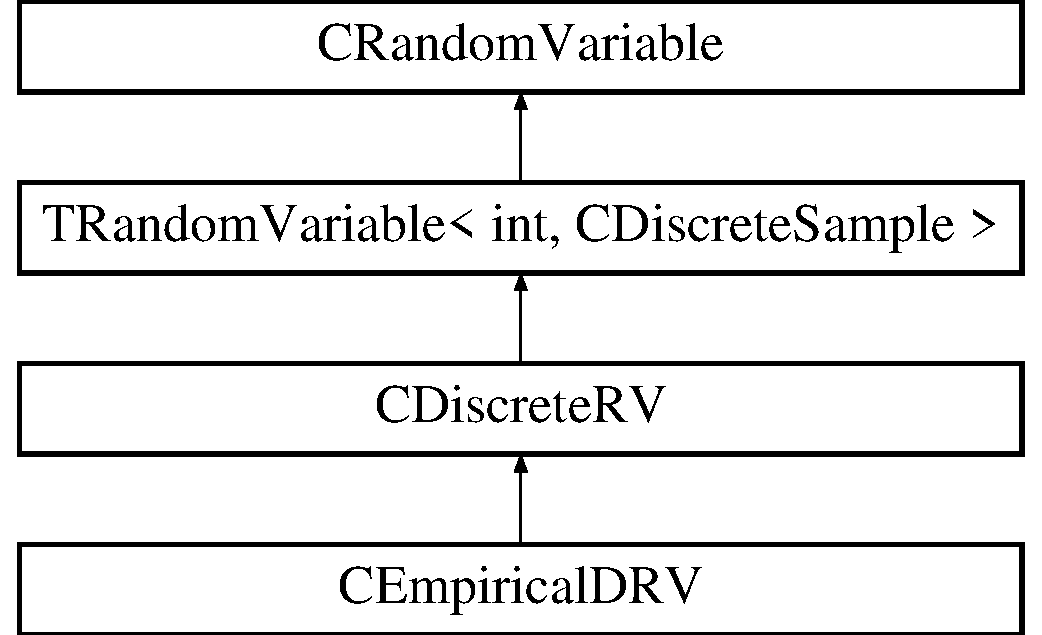
\includegraphics[height=4.000000cm]{class_c_empirical_d_r_v}
\end{center}
\end{figure}
\subsection*{Public Member Functions}
\begin{DoxyCompactItemize}
\item 
\hyperlink{class_c_empirical_d_r_v_a0b812bee54d50c33f987da3788a5da70}{C\-Empirical\-D\-R\-V} ()
\item 
virtual \hyperlink{class_c_empirical_d_r_v_af84a843f152e353a5ccac842685679c5}{$\sim$\-C\-Empirical\-D\-R\-V} ()
\item 
\hyperlink{class_c_empirical_d_r_v_a98462a73cfcab11dc73e5bb6f7244de4}{C\-Empirical\-D\-R\-V} (const \hyperlink{class_c_empirical_d_r_v}{C\-Empirical\-D\-R\-V} \&O)
\item 
virtual void \hyperlink{class_c_empirical_d_r_v_accbce4693814409137e7d77c5b36c910}{set\-Distribution} (const \hyperlink{class_c_discrete_sample}{C\-Discrete\-Sample} \&\-\_\-a\-S)
\begin{DoxyCompactList}\small\item\em Computes P\-M\-F and C\-D\-F from sample histogram. \end{DoxyCompactList}\item 
virtual double \hyperlink{class_c_empirical_d_r_v_a0bb8d31e01e419c3f8b77ecf034ca2a8}{probability} (int \-\_\-k) const 
\begin{DoxyCompactList}\small\item\em Function that returns P\-M\-F. \end{DoxyCompactList}\item 
virtual double \hyperlink{class_c_empirical_d_r_v_adab1bd8fb031410412f70d52d3ddb3e3}{cumulative} (int \-\_\-k) const 
\begin{DoxyCompactList}\small\item\em Function that returns C\-D\-F. \end{DoxyCompactList}\item 
virtual int \hyperlink{class_c_empirical_d_r_v_abb2052290e862d26d122b24aeeafa7cb}{expanded\-Size} () const 
\item 
virtual double \hyperlink{class_c_empirical_d_r_v_a85960e7ea87de4879f5893ad89b683f2}{min\-Value} () const 
\begin{DoxyCompactList}\small\item\em After expansion, number of new variables is equal to the number of categories. \end{DoxyCompactList}\item 
virtual double \hyperlink{class_c_empirical_d_r_v_a9831b815323ea8a6a60f68eda50294d8}{max\-Value} () const 
\begin{DoxyCompactList}\small\item\em Returns maximal value of the random variable. \end{DoxyCompactList}\item 
virtual double \hyperlink{class_c_empirical_d_r_v_a0d952cfaf3190a59525b774de4a1f2e3}{expected\-Value} () const 
\begin{DoxyCompactList}\small\item\em Returns expected value of the random variable. \end{DoxyCompactList}\item 
virtual \hyperlink{class_c_random_variable_a80d2a87c43847274138b51f7d713d7f1}{distributiontype} \hyperlink{class_c_empirical_d_r_v_a14227ae88985f6cdd28f7ccd3fa734e7}{distribution\-Type} () const 
\begin{DoxyCompactList}\small\item\em Returns enum type of the random variable distribution. \end{DoxyCompactList}\item 
virtual std\-::string \hyperlink{class_c_empirical_d_r_v_acfea0ba8ae0a961a27869ce8e966ba4d}{distribution\-Name} () const 
\begin{DoxyCompactList}\small\item\em Returns name of the random variable distribution. \end{DoxyCompactList}\item 
virtual Array\-Xi \hyperlink{class_c_empirical_d_r_v_a896eab1e119e990165bca4ffcb5dc7b6}{export\-Domain} () const 
\begin{DoxyCompactList}\small\item\em Exports domain of the random variable. \end{DoxyCompactList}\item 
virtual bool \hyperlink{class_c_empirical_d_r_v_a54549be13650697081979ee7ea7aae6c}{is\-Distribution\-Defined} () const 
\begin{DoxyCompactList}\small\item\em Returns true if distribution is defined, false otherwise. \end{DoxyCompactList}\item 
virtual double \hyperlink{class_c_empirical_d_r_v_a65bc76e9a58f20e0e6eec0f036e469f5}{variance} () const 
\begin{DoxyCompactList}\small\item\em Returns variance of the random variable. \end{DoxyCompactList}\end{DoxyCompactItemize}
\subsection*{Protected Member Functions}
\begin{DoxyCompactItemize}
\item 
virtual double \hyperlink{class_c_empirical_d_r_v_afa06f54ed41c6c9e743ea2d7603b6b36}{do\-Quantile} (double \-\_\-p) const 
\begin{DoxyCompactList}\small\item\em Quantile, formula implementation. \end{DoxyCompactList}\end{DoxyCompactItemize}
\subsection*{Private Member Functions}
\begin{DoxyCompactItemize}
\item 
{\footnotesize template$<$class Archive $>$ }\\void \hyperlink{class_c_empirical_d_r_v_ae17e04b165f0f575cb7ee96078faac70}{serialize} (Archive \&ar, const unsigned int version)
\end{DoxyCompactItemize}
\subsection*{Private Attributes}
\begin{DoxyCompactItemize}
\item 
Array\-Xd \hyperlink{class_c_empirical_d_r_v_a854fc8afdf4194880c978b91baff4852}{p}
\item 
Array\-Xd \hyperlink{class_c_empirical_d_r_v_aceab7d27df5fefbaaa64ab7b2e410763}{cdf}
\end{DoxyCompactItemize}
\subsection*{Friends}
\begin{DoxyCompactItemize}
\item 
class \hyperlink{class_c_empirical_d_r_v_ac98d07dd8f7b70e16ccb9a01abf56b9c}{boost\-::serialization\-::access}
\begin{DoxyCompactList}\small\item\em Boost serialization. \end{DoxyCompactList}\end{DoxyCompactItemize}
\subsection*{Additional Inherited Members}


\subsection{Detailed Description}
Class for categorical discrete random variables derived from discrete random variables. 

\subsection{Constructor \& Destructor Documentation}
\hypertarget{class_c_empirical_d_r_v_a0b812bee54d50c33f987da3788a5da70}{\index{C\-Empirical\-D\-R\-V@{C\-Empirical\-D\-R\-V}!C\-Empirical\-D\-R\-V@{C\-Empirical\-D\-R\-V}}
\index{C\-Empirical\-D\-R\-V@{C\-Empirical\-D\-R\-V}!CEmpiricalDRV@{C\-Empirical\-D\-R\-V}}
\subsubsection[{C\-Empirical\-D\-R\-V}]{\setlength{\rightskip}{0pt plus 5cm}C\-Empirical\-D\-R\-V\-::\-C\-Empirical\-D\-R\-V (
\begin{DoxyParamCaption}
{}
\end{DoxyParamCaption}
)\hspace{0.3cm}{\ttfamily [inline]}}}\label{class_c_empirical_d_r_v_a0b812bee54d50c33f987da3788a5da70}
\hypertarget{class_c_empirical_d_r_v_af84a843f152e353a5ccac842685679c5}{\index{C\-Empirical\-D\-R\-V@{C\-Empirical\-D\-R\-V}!$\sim$\-C\-Empirical\-D\-R\-V@{$\sim$\-C\-Empirical\-D\-R\-V}}
\index{$\sim$\-C\-Empirical\-D\-R\-V@{$\sim$\-C\-Empirical\-D\-R\-V}!CEmpiricalDRV@{C\-Empirical\-D\-R\-V}}
\subsubsection[{$\sim$\-C\-Empirical\-D\-R\-V}]{\setlength{\rightskip}{0pt plus 5cm}virtual C\-Empirical\-D\-R\-V\-::$\sim$\-C\-Empirical\-D\-R\-V (
\begin{DoxyParamCaption}
{}
\end{DoxyParamCaption}
)\hspace{0.3cm}{\ttfamily [inline]}, {\ttfamily [virtual]}}}\label{class_c_empirical_d_r_v_af84a843f152e353a5ccac842685679c5}
\hypertarget{class_c_empirical_d_r_v_a98462a73cfcab11dc73e5bb6f7244de4}{\index{C\-Empirical\-D\-R\-V@{C\-Empirical\-D\-R\-V}!C\-Empirical\-D\-R\-V@{C\-Empirical\-D\-R\-V}}
\index{C\-Empirical\-D\-R\-V@{C\-Empirical\-D\-R\-V}!CEmpiricalDRV@{C\-Empirical\-D\-R\-V}}
\subsubsection[{C\-Empirical\-D\-R\-V}]{\setlength{\rightskip}{0pt plus 5cm}C\-Empirical\-D\-R\-V\-::\-C\-Empirical\-D\-R\-V (
\begin{DoxyParamCaption}
\item[{const {\bf C\-Empirical\-D\-R\-V} \&}]{O}
\end{DoxyParamCaption}
)\hspace{0.3cm}{\ttfamily [inline]}}}\label{class_c_empirical_d_r_v_a98462a73cfcab11dc73e5bb6f7244de4}


\subsection{Member Function Documentation}
\hypertarget{class_c_empirical_d_r_v_adab1bd8fb031410412f70d52d3ddb3e3}{\index{C\-Empirical\-D\-R\-V@{C\-Empirical\-D\-R\-V}!cumulative@{cumulative}}
\index{cumulative@{cumulative}!CEmpiricalDRV@{C\-Empirical\-D\-R\-V}}
\subsubsection[{cumulative}]{\setlength{\rightskip}{0pt plus 5cm}virtual double C\-Empirical\-D\-R\-V\-::cumulative (
\begin{DoxyParamCaption}
\item[{int}]{\-\_\-k}
\end{DoxyParamCaption}
) const\hspace{0.3cm}{\ttfamily [inline]}, {\ttfamily [virtual]}}}\label{class_c_empirical_d_r_v_adab1bd8fb031410412f70d52d3ddb3e3}


Function that returns C\-D\-F. 

\hypertarget{class_c_empirical_d_r_v_acfea0ba8ae0a961a27869ce8e966ba4d}{\index{C\-Empirical\-D\-R\-V@{C\-Empirical\-D\-R\-V}!distribution\-Name@{distribution\-Name}}
\index{distribution\-Name@{distribution\-Name}!CEmpiricalDRV@{C\-Empirical\-D\-R\-V}}
\subsubsection[{distribution\-Name}]{\setlength{\rightskip}{0pt plus 5cm}virtual std\-::string C\-Empirical\-D\-R\-V\-::distribution\-Name (
\begin{DoxyParamCaption}
{}
\end{DoxyParamCaption}
) const\hspace{0.3cm}{\ttfamily [inline]}, {\ttfamily [virtual]}}}\label{class_c_empirical_d_r_v_acfea0ba8ae0a961a27869ce8e966ba4d}


Returns name of the random variable distribution. 



Implements \hyperlink{class_c_random_variable_a4b33eef7c56f9f1a83af01fa8ef2502b}{C\-Random\-Variable}.

\hypertarget{class_c_empirical_d_r_v_a14227ae88985f6cdd28f7ccd3fa734e7}{\index{C\-Empirical\-D\-R\-V@{C\-Empirical\-D\-R\-V}!distribution\-Type@{distribution\-Type}}
\index{distribution\-Type@{distribution\-Type}!CEmpiricalDRV@{C\-Empirical\-D\-R\-V}}
\subsubsection[{distribution\-Type}]{\setlength{\rightskip}{0pt plus 5cm}virtual {\bf distributiontype} C\-Empirical\-D\-R\-V\-::distribution\-Type (
\begin{DoxyParamCaption}
{}
\end{DoxyParamCaption}
) const\hspace{0.3cm}{\ttfamily [inline]}, {\ttfamily [virtual]}}}\label{class_c_empirical_d_r_v_a14227ae88985f6cdd28f7ccd3fa734e7}


Returns enum type of the random variable distribution. 



Implements \hyperlink{class_c_random_variable_a3b30589d41f4dd200bd40c8273cac2cd}{C\-Random\-Variable}.

\hypertarget{class_c_empirical_d_r_v_afa06f54ed41c6c9e743ea2d7603b6b36}{\index{C\-Empirical\-D\-R\-V@{C\-Empirical\-D\-R\-V}!do\-Quantile@{do\-Quantile}}
\index{do\-Quantile@{do\-Quantile}!CEmpiricalDRV@{C\-Empirical\-D\-R\-V}}
\subsubsection[{do\-Quantile}]{\setlength{\rightskip}{0pt plus 5cm}double C\-Empirical\-D\-R\-V\-::do\-Quantile (
\begin{DoxyParamCaption}
\item[{double}]{\-\_\-p}
\end{DoxyParamCaption}
) const\hspace{0.3cm}{\ttfamily [protected]}, {\ttfamily [virtual]}}}\label{class_c_empirical_d_r_v_afa06f54ed41c6c9e743ea2d7603b6b36}


Quantile, formula implementation. 



Implements \hyperlink{class_c_random_variable_a552ab36c8144d7154cbe3cd363eee65b}{C\-Random\-Variable}.

\hypertarget{class_c_empirical_d_r_v_abb2052290e862d26d122b24aeeafa7cb}{\index{C\-Empirical\-D\-R\-V@{C\-Empirical\-D\-R\-V}!expanded\-Size@{expanded\-Size}}
\index{expanded\-Size@{expanded\-Size}!CEmpiricalDRV@{C\-Empirical\-D\-R\-V}}
\subsubsection[{expanded\-Size}]{\setlength{\rightskip}{0pt plus 5cm}virtual int C\-Empirical\-D\-R\-V\-::expanded\-Size (
\begin{DoxyParamCaption}
{}
\end{DoxyParamCaption}
) const\hspace{0.3cm}{\ttfamily [inline]}, {\ttfamily [virtual]}}}\label{class_c_empirical_d_r_v_abb2052290e862d26d122b24aeeafa7cb}


Reimplemented from \hyperlink{class_c_random_variable_ada091c2895cf25a75ac8aacecb5da47f}{C\-Random\-Variable}.

\hypertarget{class_c_empirical_d_r_v_a0d952cfaf3190a59525b774de4a1f2e3}{\index{C\-Empirical\-D\-R\-V@{C\-Empirical\-D\-R\-V}!expected\-Value@{expected\-Value}}
\index{expected\-Value@{expected\-Value}!CEmpiricalDRV@{C\-Empirical\-D\-R\-V}}
\subsubsection[{expected\-Value}]{\setlength{\rightskip}{0pt plus 5cm}virtual double C\-Empirical\-D\-R\-V\-::expected\-Value (
\begin{DoxyParamCaption}
{}
\end{DoxyParamCaption}
) const\hspace{0.3cm}{\ttfamily [inline]}, {\ttfamily [virtual]}}}\label{class_c_empirical_d_r_v_a0d952cfaf3190a59525b774de4a1f2e3}


Returns expected value of the random variable. 



Implements \hyperlink{class_c_random_variable_a6e5490d17f2b6abcf9922c8b1bd6d4ed}{C\-Random\-Variable}.

\hypertarget{class_c_empirical_d_r_v_a896eab1e119e990165bca4ffcb5dc7b6}{\index{C\-Empirical\-D\-R\-V@{C\-Empirical\-D\-R\-V}!export\-Domain@{export\-Domain}}
\index{export\-Domain@{export\-Domain}!CEmpiricalDRV@{C\-Empirical\-D\-R\-V}}
\subsubsection[{export\-Domain}]{\setlength{\rightskip}{0pt plus 5cm}Array\-Xi C\-Empirical\-D\-R\-V\-::export\-Domain (
\begin{DoxyParamCaption}
{}
\end{DoxyParamCaption}
) const\hspace{0.3cm}{\ttfamily [virtual]}}}\label{class_c_empirical_d_r_v_a896eab1e119e990165bca4ffcb5dc7b6}


Exports domain of the random variable. 



Implements \hyperlink{class_t_random_variable_a37fc52d5fa37493a353887242d279a27}{T\-Random\-Variable$<$ t, T $>$}.

\hypertarget{class_c_empirical_d_r_v_a54549be13650697081979ee7ea7aae6c}{\index{C\-Empirical\-D\-R\-V@{C\-Empirical\-D\-R\-V}!is\-Distribution\-Defined@{is\-Distribution\-Defined}}
\index{is\-Distribution\-Defined@{is\-Distribution\-Defined}!CEmpiricalDRV@{C\-Empirical\-D\-R\-V}}
\subsubsection[{is\-Distribution\-Defined}]{\setlength{\rightskip}{0pt plus 5cm}virtual bool C\-Empirical\-D\-R\-V\-::is\-Distribution\-Defined (
\begin{DoxyParamCaption}
{}
\end{DoxyParamCaption}
) const\hspace{0.3cm}{\ttfamily [inline]}, {\ttfamily [virtual]}}}\label{class_c_empirical_d_r_v_a54549be13650697081979ee7ea7aae6c}


Returns true if distribution is defined, false otherwise. 



Reimplemented from \hyperlink{class_c_random_variable_a60e88c15450ab21dea6bef00d8836da7}{C\-Random\-Variable}.

\hypertarget{class_c_empirical_d_r_v_a9831b815323ea8a6a60f68eda50294d8}{\index{C\-Empirical\-D\-R\-V@{C\-Empirical\-D\-R\-V}!max\-Value@{max\-Value}}
\index{max\-Value@{max\-Value}!CEmpiricalDRV@{C\-Empirical\-D\-R\-V}}
\subsubsection[{max\-Value}]{\setlength{\rightskip}{0pt plus 5cm}virtual double C\-Empirical\-D\-R\-V\-::max\-Value (
\begin{DoxyParamCaption}
{}
\end{DoxyParamCaption}
) const\hspace{0.3cm}{\ttfamily [inline]}, {\ttfamily [virtual]}}}\label{class_c_empirical_d_r_v_a9831b815323ea8a6a60f68eda50294d8}


Returns maximal value of the random variable. 



Implements \hyperlink{class_c_random_variable_a48a5e98363d866f1f46568ed658479ad}{C\-Random\-Variable}.

\hypertarget{class_c_empirical_d_r_v_a85960e7ea87de4879f5893ad89b683f2}{\index{C\-Empirical\-D\-R\-V@{C\-Empirical\-D\-R\-V}!min\-Value@{min\-Value}}
\index{min\-Value@{min\-Value}!CEmpiricalDRV@{C\-Empirical\-D\-R\-V}}
\subsubsection[{min\-Value}]{\setlength{\rightskip}{0pt plus 5cm}virtual double C\-Empirical\-D\-R\-V\-::min\-Value (
\begin{DoxyParamCaption}
{}
\end{DoxyParamCaption}
) const\hspace{0.3cm}{\ttfamily [inline]}, {\ttfamily [virtual]}}}\label{class_c_empirical_d_r_v_a85960e7ea87de4879f5893ad89b683f2}


After expansion, number of new variables is equal to the number of categories. 

Returns minimal value of the random variable. 

Implements \hyperlink{class_c_random_variable_a233ddd2eedb51b09a04a8c330646f356}{C\-Random\-Variable}.

\hypertarget{class_c_empirical_d_r_v_a0bb8d31e01e419c3f8b77ecf034ca2a8}{\index{C\-Empirical\-D\-R\-V@{C\-Empirical\-D\-R\-V}!probability@{probability}}
\index{probability@{probability}!CEmpiricalDRV@{C\-Empirical\-D\-R\-V}}
\subsubsection[{probability}]{\setlength{\rightskip}{0pt plus 5cm}virtual double C\-Empirical\-D\-R\-V\-::probability (
\begin{DoxyParamCaption}
\item[{int}]{\-\_\-k}
\end{DoxyParamCaption}
) const\hspace{0.3cm}{\ttfamily [inline]}, {\ttfamily [virtual]}}}\label{class_c_empirical_d_r_v_a0bb8d31e01e419c3f8b77ecf034ca2a8}


Function that returns P\-M\-F. 

\hypertarget{class_c_empirical_d_r_v_ae17e04b165f0f575cb7ee96078faac70}{\index{C\-Empirical\-D\-R\-V@{C\-Empirical\-D\-R\-V}!serialize@{serialize}}
\index{serialize@{serialize}!CEmpiricalDRV@{C\-Empirical\-D\-R\-V}}
\subsubsection[{serialize}]{\setlength{\rightskip}{0pt plus 5cm}template$<$class Archive $>$ void C\-Empirical\-D\-R\-V\-::serialize (
\begin{DoxyParamCaption}
\item[{Archive \&}]{ar, }
\item[{const unsigned int}]{version}
\end{DoxyParamCaption}
)\hspace{0.3cm}{\ttfamily [private]}}}\label{class_c_empirical_d_r_v_ae17e04b165f0f575cb7ee96078faac70}
\hypertarget{class_c_empirical_d_r_v_accbce4693814409137e7d77c5b36c910}{\index{C\-Empirical\-D\-R\-V@{C\-Empirical\-D\-R\-V}!set\-Distribution@{set\-Distribution}}
\index{set\-Distribution@{set\-Distribution}!CEmpiricalDRV@{C\-Empirical\-D\-R\-V}}
\subsubsection[{set\-Distribution}]{\setlength{\rightskip}{0pt plus 5cm}void C\-Empirical\-D\-R\-V\-::set\-Distribution (
\begin{DoxyParamCaption}
\item[{const {\bf C\-Discrete\-Sample} \&}]{\-\_\-a\-S}
\end{DoxyParamCaption}
)\hspace{0.3cm}{\ttfamily [virtual]}}}\label{class_c_empirical_d_r_v_accbce4693814409137e7d77c5b36c910}


Computes P\-M\-F and C\-D\-F from sample histogram. 

\hypertarget{class_c_empirical_d_r_v_a65bc76e9a58f20e0e6eec0f036e469f5}{\index{C\-Empirical\-D\-R\-V@{C\-Empirical\-D\-R\-V}!variance@{variance}}
\index{variance@{variance}!CEmpiricalDRV@{C\-Empirical\-D\-R\-V}}
\subsubsection[{variance}]{\setlength{\rightskip}{0pt plus 5cm}virtual double C\-Empirical\-D\-R\-V\-::variance (
\begin{DoxyParamCaption}
{}
\end{DoxyParamCaption}
) const\hspace{0.3cm}{\ttfamily [inline]}, {\ttfamily [virtual]}}}\label{class_c_empirical_d_r_v_a65bc76e9a58f20e0e6eec0f036e469f5}


Returns variance of the random variable. 



Implements \hyperlink{class_c_random_variable_a3b0b87c4aab74c0406cd8321b8b96747}{C\-Random\-Variable}.



\subsection{Friends And Related Function Documentation}
\hypertarget{class_c_empirical_d_r_v_ac98d07dd8f7b70e16ccb9a01abf56b9c}{\index{C\-Empirical\-D\-R\-V@{C\-Empirical\-D\-R\-V}!boost\-::serialization\-::access@{boost\-::serialization\-::access}}
\index{boost\-::serialization\-::access@{boost\-::serialization\-::access}!CEmpiricalDRV@{C\-Empirical\-D\-R\-V}}
\subsubsection[{boost\-::serialization\-::access}]{\setlength{\rightskip}{0pt plus 5cm}friend class boost\-::serialization\-::access\hspace{0.3cm}{\ttfamily [friend]}}}\label{class_c_empirical_d_r_v_ac98d07dd8f7b70e16ccb9a01abf56b9c}


Boost serialization. 



\subsection{Member Data Documentation}
\hypertarget{class_c_empirical_d_r_v_aceab7d27df5fefbaaa64ab7b2e410763}{\index{C\-Empirical\-D\-R\-V@{C\-Empirical\-D\-R\-V}!cdf@{cdf}}
\index{cdf@{cdf}!CEmpiricalDRV@{C\-Empirical\-D\-R\-V}}
\subsubsection[{cdf}]{\setlength{\rightskip}{0pt plus 5cm}Array\-Xd C\-Empirical\-D\-R\-V\-::cdf\hspace{0.3cm}{\ttfamily [private]}}}\label{class_c_empirical_d_r_v_aceab7d27df5fefbaaa64ab7b2e410763}
P\-M\-F (p) and C\-D\-F (cdf) data. \hypertarget{class_c_empirical_d_r_v_a854fc8afdf4194880c978b91baff4852}{\index{C\-Empirical\-D\-R\-V@{C\-Empirical\-D\-R\-V}!p@{p}}
\index{p@{p}!CEmpiricalDRV@{C\-Empirical\-D\-R\-V}}
\subsubsection[{p}]{\setlength{\rightskip}{0pt plus 5cm}Array\-Xd C\-Empirical\-D\-R\-V\-::p\hspace{0.3cm}{\ttfamily [private]}}}\label{class_c_empirical_d_r_v_a854fc8afdf4194880c978b91baff4852}


The documentation for this class was generated from the following files\-:\begin{DoxyCompactItemize}
\item 
C\-:/\-Development/core/\hyperlink{_random_variable_8h}{Random\-Variable.\-h}\item 
C\-:/\-Development/core/\hyperlink{_random_variable_8cpp}{Random\-Variable.\-cpp}\end{DoxyCompactItemize}

\hypertarget{class_go_s_u_m_1_1_c_eps_svr_s_a_m}{\section{Go\-S\-U\-M\-:\-:C\-Eps\-Svr\-S\-A\-M Class Reference}
\label{class_go_s_u_m_1_1_c_eps_svr_s_a_m}\index{Go\-S\-U\-M\-::\-C\-Eps\-Svr\-S\-A\-M@{Go\-S\-U\-M\-::\-C\-Eps\-Svr\-S\-A\-M}}
}


Class for the analyitical model for single output state, epsilon-\/\-S\-V\-R type.  




{\ttfamily \#include $<$Analytical\-Model.\-h$>$}

Inheritance diagram for Go\-S\-U\-M\-:\-:C\-Eps\-Svr\-S\-A\-M\-:\begin{figure}[H]
\begin{center}
\leavevmode
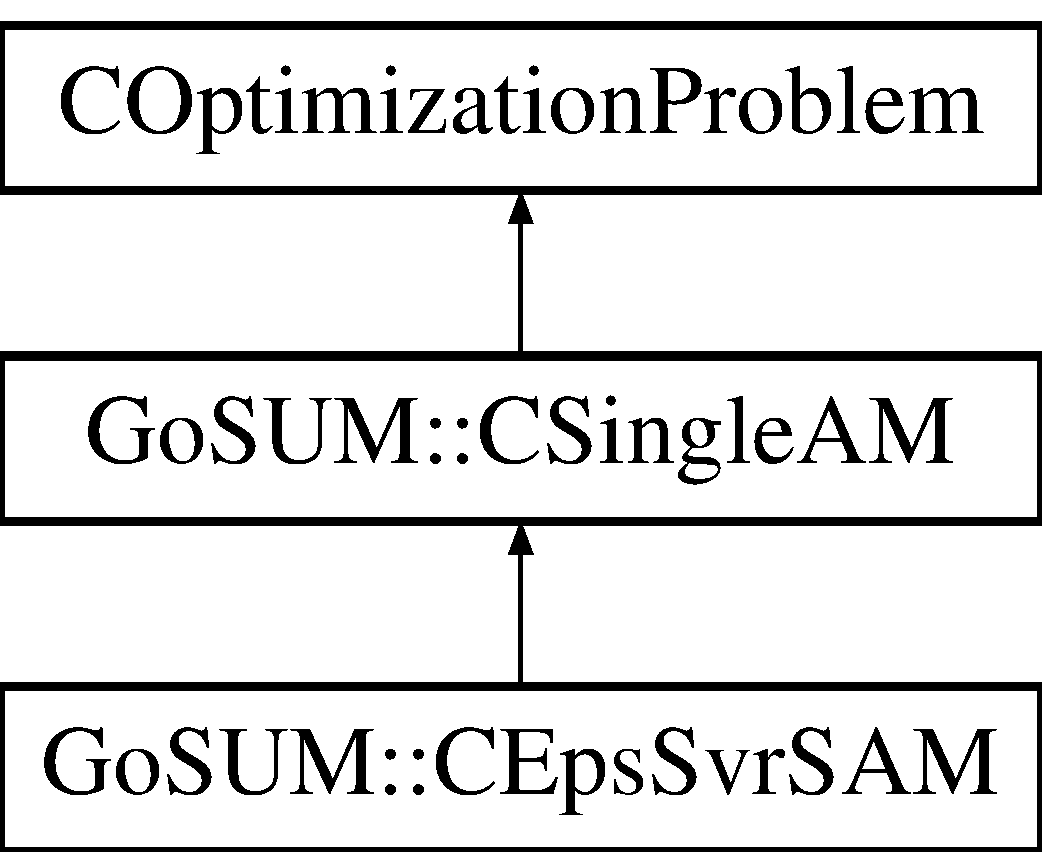
\includegraphics[height=3.000000cm]{class_go_s_u_m_1_1_c_eps_svr_s_a_m}
\end{center}
\end{figure}
\subsection*{Public Member Functions}
\begin{DoxyCompactItemize}
\item 
\hyperlink{class_go_s_u_m_1_1_c_eps_svr_s_a_m_aa3b33675066457d185fa2c0cab6edc4f}{C\-Eps\-Svr\-S\-A\-M} ()
\item 
virtual \hyperlink{class_go_s_u_m_1_1_c_eps_svr_s_a_m_a5490c6b8316c4fdf4b2a5124d50532a4}{$\sim$\-C\-Eps\-Svr\-S\-A\-M} ()
\item 
virtual void \hyperlink{class_go_s_u_m_1_1_c_eps_svr_s_a_m_a4ffdcbae7411ad49822e35957bbe2f44}{open\-Optimization} ()
\begin{DoxyCompactList}\small\item\em Opens optmization. \end{DoxyCompactList}\item 
virtual void \hyperlink{class_go_s_u_m_1_1_c_eps_svr_s_a_m_a44286934f7dad34f93aeefecda8bad18}{optimization\-Point2\-S\-V\-M\-Param} (const Array\-Xd \&ov)
\begin{DoxyCompactList}\small\item\em Converts optimization point to S\-V\-M parameters. \end{DoxyCompactList}\end{DoxyCompactItemize}
\subsection*{Protected Member Functions}
\begin{DoxyCompactItemize}
\item 
{\footnotesize template$<$class Archive $>$ }\\void \hyperlink{class_go_s_u_m_1_1_c_eps_svr_s_a_m_aa981fefdc8dc0376e7fc5175cb81f66e}{serialize} (Archive \&ar, const unsigned int version)
\end{DoxyCompactItemize}
\subsection*{Friends}
\begin{DoxyCompactItemize}
\item 
class \hyperlink{class_go_s_u_m_1_1_c_eps_svr_s_a_m_ac98d07dd8f7b70e16ccb9a01abf56b9c}{boost\-::serialization\-::access}
\begin{DoxyCompactList}\small\item\em Boost serialization. \end{DoxyCompactList}\end{DoxyCompactItemize}
\subsection*{Additional Inherited Members}


\subsection{Detailed Description}
Class for the analyitical model for single output state, epsilon-\/\-S\-V\-R type. 

\subsection{Constructor \& Destructor Documentation}
\hypertarget{class_go_s_u_m_1_1_c_eps_svr_s_a_m_aa3b33675066457d185fa2c0cab6edc4f}{\index{Go\-S\-U\-M\-::\-C\-Eps\-Svr\-S\-A\-M@{Go\-S\-U\-M\-::\-C\-Eps\-Svr\-S\-A\-M}!C\-Eps\-Svr\-S\-A\-M@{C\-Eps\-Svr\-S\-A\-M}}
\index{C\-Eps\-Svr\-S\-A\-M@{C\-Eps\-Svr\-S\-A\-M}!GoSUM::CEpsSvrSAM@{Go\-S\-U\-M\-::\-C\-Eps\-Svr\-S\-A\-M}}
\subsubsection[{C\-Eps\-Svr\-S\-A\-M}]{\setlength{\rightskip}{0pt plus 5cm}Go\-S\-U\-M\-::\-C\-Eps\-Svr\-S\-A\-M\-::\-C\-Eps\-Svr\-S\-A\-M (
\begin{DoxyParamCaption}
{}
\end{DoxyParamCaption}
)\hspace{0.3cm}{\ttfamily [inline]}}}\label{class_go_s_u_m_1_1_c_eps_svr_s_a_m_aa3b33675066457d185fa2c0cab6edc4f}
\hypertarget{class_go_s_u_m_1_1_c_eps_svr_s_a_m_a5490c6b8316c4fdf4b2a5124d50532a4}{\index{Go\-S\-U\-M\-::\-C\-Eps\-Svr\-S\-A\-M@{Go\-S\-U\-M\-::\-C\-Eps\-Svr\-S\-A\-M}!$\sim$\-C\-Eps\-Svr\-S\-A\-M@{$\sim$\-C\-Eps\-Svr\-S\-A\-M}}
\index{$\sim$\-C\-Eps\-Svr\-S\-A\-M@{$\sim$\-C\-Eps\-Svr\-S\-A\-M}!GoSUM::CEpsSvrSAM@{Go\-S\-U\-M\-::\-C\-Eps\-Svr\-S\-A\-M}}
\subsubsection[{$\sim$\-C\-Eps\-Svr\-S\-A\-M}]{\setlength{\rightskip}{0pt plus 5cm}virtual Go\-S\-U\-M\-::\-C\-Eps\-Svr\-S\-A\-M\-::$\sim$\-C\-Eps\-Svr\-S\-A\-M (
\begin{DoxyParamCaption}
{}
\end{DoxyParamCaption}
)\hspace{0.3cm}{\ttfamily [inline]}, {\ttfamily [virtual]}}}\label{class_go_s_u_m_1_1_c_eps_svr_s_a_m_a5490c6b8316c4fdf4b2a5124d50532a4}


\subsection{Member Function Documentation}
\hypertarget{class_go_s_u_m_1_1_c_eps_svr_s_a_m_a4ffdcbae7411ad49822e35957bbe2f44}{\index{Go\-S\-U\-M\-::\-C\-Eps\-Svr\-S\-A\-M@{Go\-S\-U\-M\-::\-C\-Eps\-Svr\-S\-A\-M}!open\-Optimization@{open\-Optimization}}
\index{open\-Optimization@{open\-Optimization}!GoSUM::CEpsSvrSAM@{Go\-S\-U\-M\-::\-C\-Eps\-Svr\-S\-A\-M}}
\subsubsection[{open\-Optimization}]{\setlength{\rightskip}{0pt plus 5cm}void Go\-S\-U\-M\-::\-C\-Eps\-Svr\-S\-A\-M\-::open\-Optimization (
\begin{DoxyParamCaption}
{}
\end{DoxyParamCaption}
)\hspace{0.3cm}{\ttfamily [virtual]}}}\label{class_go_s_u_m_1_1_c_eps_svr_s_a_m_a4ffdcbae7411ad49822e35957bbe2f44}


Opens optmization. 



Reimplemented from \hyperlink{class_go_s_u_m_1_1_c_single_a_m_acdaa489065049af967092e904004f299}{Go\-S\-U\-M\-::\-C\-Single\-A\-M}.

\hypertarget{class_go_s_u_m_1_1_c_eps_svr_s_a_m_a44286934f7dad34f93aeefecda8bad18}{\index{Go\-S\-U\-M\-::\-C\-Eps\-Svr\-S\-A\-M@{Go\-S\-U\-M\-::\-C\-Eps\-Svr\-S\-A\-M}!optimization\-Point2\-S\-V\-M\-Param@{optimization\-Point2\-S\-V\-M\-Param}}
\index{optimization\-Point2\-S\-V\-M\-Param@{optimization\-Point2\-S\-V\-M\-Param}!GoSUM::CEpsSvrSAM@{Go\-S\-U\-M\-::\-C\-Eps\-Svr\-S\-A\-M}}
\subsubsection[{optimization\-Point2\-S\-V\-M\-Param}]{\setlength{\rightskip}{0pt plus 5cm}void Go\-S\-U\-M\-::\-C\-Eps\-Svr\-S\-A\-M\-::optimization\-Point2\-S\-V\-M\-Param (
\begin{DoxyParamCaption}
\item[{const Array\-Xd \&}]{ov}
\end{DoxyParamCaption}
)\hspace{0.3cm}{\ttfamily [virtual]}}}\label{class_go_s_u_m_1_1_c_eps_svr_s_a_m_a44286934f7dad34f93aeefecda8bad18}


Converts optimization point to S\-V\-M parameters. 



Reimplemented from \hyperlink{class_go_s_u_m_1_1_c_single_a_m_a28c4026a43409c73e27acbdabfff35ee}{Go\-S\-U\-M\-::\-C\-Single\-A\-M}.

\hypertarget{class_go_s_u_m_1_1_c_eps_svr_s_a_m_aa981fefdc8dc0376e7fc5175cb81f66e}{\index{Go\-S\-U\-M\-::\-C\-Eps\-Svr\-S\-A\-M@{Go\-S\-U\-M\-::\-C\-Eps\-Svr\-S\-A\-M}!serialize@{serialize}}
\index{serialize@{serialize}!GoSUM::CEpsSvrSAM@{Go\-S\-U\-M\-::\-C\-Eps\-Svr\-S\-A\-M}}
\subsubsection[{serialize}]{\setlength{\rightskip}{0pt plus 5cm}template$<$class Archive $>$ void Go\-S\-U\-M\-::\-C\-Eps\-Svr\-S\-A\-M\-::serialize (
\begin{DoxyParamCaption}
\item[{Archive \&}]{ar, }
\item[{const unsigned int}]{version}
\end{DoxyParamCaption}
)\hspace{0.3cm}{\ttfamily [protected]}}}\label{class_go_s_u_m_1_1_c_eps_svr_s_a_m_aa981fefdc8dc0376e7fc5175cb81f66e}


Reimplemented from \hyperlink{class_go_s_u_m_1_1_c_single_a_m_a761e514fefeb7324e5509571f1be3848}{Go\-S\-U\-M\-::\-C\-Single\-A\-M}.



\subsection{Friends And Related Function Documentation}
\hypertarget{class_go_s_u_m_1_1_c_eps_svr_s_a_m_ac98d07dd8f7b70e16ccb9a01abf56b9c}{\index{Go\-S\-U\-M\-::\-C\-Eps\-Svr\-S\-A\-M@{Go\-S\-U\-M\-::\-C\-Eps\-Svr\-S\-A\-M}!boost\-::serialization\-::access@{boost\-::serialization\-::access}}
\index{boost\-::serialization\-::access@{boost\-::serialization\-::access}!GoSUM::CEpsSvrSAM@{Go\-S\-U\-M\-::\-C\-Eps\-Svr\-S\-A\-M}}
\subsubsection[{boost\-::serialization\-::access}]{\setlength{\rightskip}{0pt plus 5cm}friend class boost\-::serialization\-::access\hspace{0.3cm}{\ttfamily [friend]}}}\label{class_go_s_u_m_1_1_c_eps_svr_s_a_m_ac98d07dd8f7b70e16ccb9a01abf56b9c}


Boost serialization. 



The documentation for this class was generated from the following files\-:\begin{DoxyCompactItemize}
\item 
C\-:/\-Development/core/\hyperlink{_analytical_model_8h}{Analytical\-Model.\-h}\item 
C\-:/\-Development/core/\hyperlink{_analytical_model_8cpp}{Analytical\-Model.\-cpp}\end{DoxyCompactItemize}

\hypertarget{class_go_s_u_m_1_1_c_evaluator}{\section{Go\-S\-U\-M\-:\-:C\-Evaluator Class Reference}
\label{class_go_s_u_m_1_1_c_evaluator}\index{Go\-S\-U\-M\-::\-C\-Evaluator@{Go\-S\-U\-M\-::\-C\-Evaluator}}
}


Class for \hyperlink{struct_go_s_u_m}{Go\-S\-U\-M} model evaluator.  




{\ttfamily \#include $<$Original\-Model.\-h$>$}

Inheritance diagram for Go\-S\-U\-M\-:\-:C\-Evaluator\-:\begin{figure}[H]
\begin{center}
\leavevmode
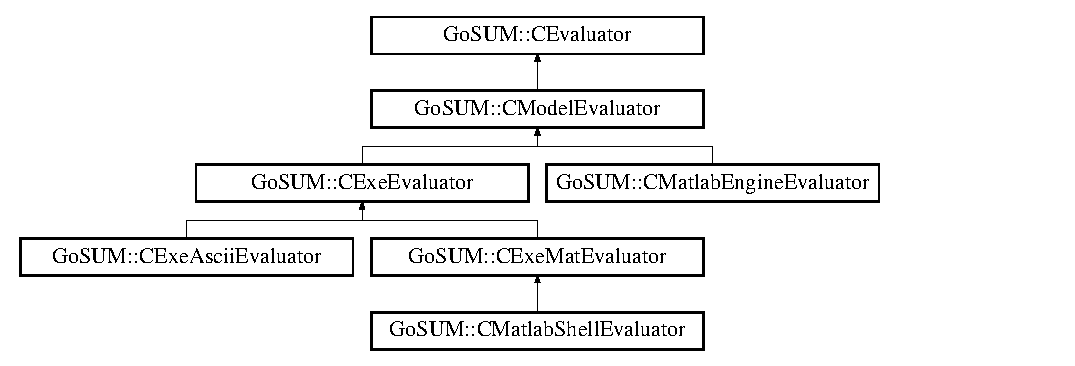
\includegraphics[height=4.465710cm]{class_go_s_u_m_1_1_c_evaluator}
\end{center}
\end{figure}
\subsection*{Public Types}
\begin{DoxyCompactItemize}
\item 
enum \hyperlink{class_go_s_u_m_1_1_c_evaluator_a50058cbf6a2c5b94677045ee02b67db2}{evaluatortype} \{ \hyperlink{class_go_s_u_m_1_1_c_evaluator_a50058cbf6a2c5b94677045ee02b67db2aedc52357596b711794cd5bac1aaf813f}{exeascii}, 
\hyperlink{class_go_s_u_m_1_1_c_evaluator_a50058cbf6a2c5b94677045ee02b67db2a0d57d51307eeadeacbfc6714ba003cf6}{exemat}, 
\hyperlink{class_go_s_u_m_1_1_c_evaluator_a50058cbf6a2c5b94677045ee02b67db2a5d73ae80ffe4497b6d5989bf05321da9}{matlabshell}, 
\hyperlink{class_go_s_u_m_1_1_c_evaluator_a50058cbf6a2c5b94677045ee02b67db2aff1ccecb2d33139472f45b9b1e2e63c5}{matlabengine}
 \}
\end{DoxyCompactItemize}
\subsection*{Public Member Functions}
\begin{DoxyCompactItemize}
\item 
\hyperlink{class_go_s_u_m_1_1_c_evaluator_ab61245188502828a2fdfa2f16fba9dea}{C\-Evaluator} ()
\item 
virtual \hyperlink{class_go_s_u_m_1_1_c_evaluator_a4b7f440821f62b112af66bae55f800b6}{$\sim$\-C\-Evaluator} ()
\end{DoxyCompactItemize}
\subsection*{Static Public Member Functions}
\begin{DoxyCompactItemize}
\item 
static void \hyperlink{class_go_s_u_m_1_1_c_evaluator_a8dd7cff8a0d0ce0857f77769a24b67ab}{clear} ()
\begin{DoxyCompactList}\small\item\em Clears data. \end{DoxyCompactList}\item 
static int \hyperlink{class_go_s_u_m_1_1_c_evaluator_abd38361870902bdcdf41543f1c416e61}{Thread\-Size} ()
\begin{DoxyCompactList}\small\item\em Returns thread size. \end{DoxyCompactList}\item 
static void \hyperlink{class_go_s_u_m_1_1_c_evaluator_a2d37e82e77ebaf2c9dd8fa33bbe5f62a}{Set\-Thread\-Size} (int \-\_\-trd\-N)
\begin{DoxyCompactList}\small\item\em Sets thread size. \end{DoxyCompactList}\item 
static void \hyperlink{class_go_s_u_m_1_1_c_evaluator_af5efaa184dbd5675ffa9fd6e711a5855}{Set\-Type} (\hyperlink{class_go_s_u_m_1_1_c_evaluator_a50058cbf6a2c5b94677045ee02b67db2}{Go\-S\-U\-M\-::\-C\-Evaluator\-::evaluatortype} \-\_\-type)
\begin{DoxyCompactList}\small\item\em Sets evaluator type. \end{DoxyCompactList}\item 
static void \hyperlink{class_go_s_u_m_1_1_c_evaluator_ae5283dc3a7955d23941eff2f5571499c}{Set\-External\-Evaluator} (const std\-::string \&\-\_\-filename)
\begin{DoxyCompactList}\small\item\em Sets external evaluator. \end{DoxyCompactList}\item 
static \hyperlink{class_go_s_u_m_1_1_c_evaluator_a50058cbf6a2c5b94677045ee02b67db2}{evaluatortype} \hyperlink{class_go_s_u_m_1_1_c_evaluator_ac1826721f6a9f7d747d75fc4c95f8b18}{Type} (const std\-::string \&\-\_\-stype)
\begin{DoxyCompactList}\small\item\em Converts evaluator type name to evaluator type enumerator. \end{DoxyCompactList}\item 
static \hyperlink{class_go_s_u_m_1_1_c_evaluator_a50058cbf6a2c5b94677045ee02b67db2}{evaluatortype} \hyperlink{class_go_s_u_m_1_1_c_evaluator_a134a607068d97d9fba70442e53e19516}{Type} ()
\begin{DoxyCompactList}\small\item\em Returns evalutor type. \end{DoxyCompactList}\item 
static \hyperlink{class_go_s_u_m_1_1_c_model_evaluator}{Go\-S\-U\-M\-::\-C\-Model\-Evaluator} $\ast$ \hyperlink{class_go_s_u_m_1_1_c_evaluator_a326cfc86daad6593f5f4b481f4b2a374}{New} (const \hyperlink{class_go_s_u_m_1_1_c_input_parameters}{C\-Input\-Parameters} $\ast$\-\_\-p\-I\-P, \hyperlink{class_go_s_u_m_1_1_c_output_states}{C\-Output\-States} $\ast$\-\_\-p\-O\-S, int \-\_\-trd\-I=0)
\begin{DoxyCompactList}\small\item\em Returns new model evalutor. \end{DoxyCompactList}\item 
static std\-::string \hyperlink{class_go_s_u_m_1_1_c_evaluator_a9c16bc0381ea164e080dcf379e08bcbc}{External\-Evaluator} ()
\begin{DoxyCompactList}\small\item\em Returns full path of the external evalautor. \end{DoxyCompactList}\item 
static std\-::string \hyperlink{class_go_s_u_m_1_1_c_evaluator_a2f968952d01303754d69977cd11252ab}{External\-Evaluator\-Folder} ()
\begin{DoxyCompactList}\small\item\em Returns folder of the external evalautor. \end{DoxyCompactList}\end{DoxyCompactItemize}
\subsection*{Public Attributes}
\begin{DoxyCompactItemize}
\item 
boost\-::signal$<$ void()$>$ \hyperlink{class_go_s_u_m_1_1_c_evaluator_ad7c33e830a5ebddbe7a0ddf873b615fe}{evaluating\-Progressed}
\begin{DoxyCompactList}\small\item\em Signal for evaluation progress, emitted after single evaluation. \end{DoxyCompactList}\end{DoxyCompactItemize}
\subsection*{Protected Member Functions}
\begin{DoxyCompactItemize}
\item 
{\footnotesize template$<$class Archive $>$ }\\void \hyperlink{class_go_s_u_m_1_1_c_evaluator_a4b1d1f83a5a9280b7cbaf65adcc2f7df}{serialize} (Archive \&ar, const unsigned int version)
\end{DoxyCompactItemize}
\subsection*{Static Protected Attributes}
\begin{DoxyCompactItemize}
\item 
static int \hyperlink{class_go_s_u_m_1_1_c_evaluator_ad38d33c6185379f37aab2da03b471f8f}{trd\-N} = 1
\begin{DoxyCompactList}\small\item\em Total number of threads and id of the particular thread this class runs in. \end{DoxyCompactList}\item 
static enum \hyperlink{class_go_s_u_m_1_1_c_evaluator_a50058cbf6a2c5b94677045ee02b67db2}{evaluatortype} \hyperlink{class_go_s_u_m_1_1_c_evaluator_ad6fd7df40c7a7b4ccc9adec41d7442f8}{type}
\begin{DoxyCompactList}\small\item\em Holds type of the evalautor. \end{DoxyCompactList}\item 
static std\-::string \hyperlink{class_go_s_u_m_1_1_c_evaluator_aef57af904e0ce1e60ed12034a369a994}{path}
\item 
static std\-::string \hyperlink{class_go_s_u_m_1_1_c_evaluator_a6e043161a2f3bf2c3065d4db8f84378e}{exe}
\item 
static std\-::string \hyperlink{class_go_s_u_m_1_1_c_evaluator_ae7b62285dd724277532c74a216750539}{in}
\item 
static std\-::string \hyperlink{class_go_s_u_m_1_1_c_evaluator_ad55ba1b2c42a31ecb493a64daf8e9a4e}{out}
\item 
static std\-::string \hyperlink{class_go_s_u_m_1_1_c_evaluator_acacec0607130855ea0840ab2ef7b6418}{ext}
\end{DoxyCompactItemize}
\subsection*{Friends}
\begin{DoxyCompactItemize}
\item 
class \hyperlink{class_go_s_u_m_1_1_c_evaluator_ac98d07dd8f7b70e16ccb9a01abf56b9c}{boost\-::serialization\-::access}
\begin{DoxyCompactList}\small\item\em Boost serialization. \end{DoxyCompactList}\end{DoxyCompactItemize}


\subsection{Detailed Description}
Class for \hyperlink{struct_go_s_u_m}{Go\-S\-U\-M} model evaluator. 

\subsection{Member Enumeration Documentation}
\hypertarget{class_go_s_u_m_1_1_c_evaluator_a50058cbf6a2c5b94677045ee02b67db2}{\index{Go\-S\-U\-M\-::\-C\-Evaluator@{Go\-S\-U\-M\-::\-C\-Evaluator}!evaluatortype@{evaluatortype}}
\index{evaluatortype@{evaluatortype}!GoSUM::CEvaluator@{Go\-S\-U\-M\-::\-C\-Evaluator}}
\subsubsection[{evaluatortype}]{\setlength{\rightskip}{0pt plus 5cm}enum {\bf Go\-S\-U\-M\-::\-C\-Evaluator\-::evaluatortype}}}\label{class_go_s_u_m_1_1_c_evaluator_a50058cbf6a2c5b94677045ee02b67db2}
\begin{Desc}
\item[Enumerator\-: ]\par
\begin{description}
\index{exeascii@{exeascii}!Go\-S\-U\-M\-::\-C\-Evaluator@{Go\-S\-U\-M\-::\-C\-Evaluator}}\index{Go\-S\-U\-M\-::\-C\-Evaluator@{Go\-S\-U\-M\-::\-C\-Evaluator}!exeascii@{exeascii}}\item[{\em 
\hypertarget{class_go_s_u_m_1_1_c_evaluator_a50058cbf6a2c5b94677045ee02b67db2aedc52357596b711794cd5bac1aaf813f}{exeascii}\label{class_go_s_u_m_1_1_c_evaluator_a50058cbf6a2c5b94677045ee02b67db2aedc52357596b711794cd5bac1aaf813f}
}]\index{exemat@{exemat}!Go\-S\-U\-M\-::\-C\-Evaluator@{Go\-S\-U\-M\-::\-C\-Evaluator}}\index{Go\-S\-U\-M\-::\-C\-Evaluator@{Go\-S\-U\-M\-::\-C\-Evaluator}!exemat@{exemat}}\item[{\em 
\hypertarget{class_go_s_u_m_1_1_c_evaluator_a50058cbf6a2c5b94677045ee02b67db2a0d57d51307eeadeacbfc6714ba003cf6}{exemat}\label{class_go_s_u_m_1_1_c_evaluator_a50058cbf6a2c5b94677045ee02b67db2a0d57d51307eeadeacbfc6714ba003cf6}
}]\index{matlabshell@{matlabshell}!Go\-S\-U\-M\-::\-C\-Evaluator@{Go\-S\-U\-M\-::\-C\-Evaluator}}\index{Go\-S\-U\-M\-::\-C\-Evaluator@{Go\-S\-U\-M\-::\-C\-Evaluator}!matlabshell@{matlabshell}}\item[{\em 
\hypertarget{class_go_s_u_m_1_1_c_evaluator_a50058cbf6a2c5b94677045ee02b67db2a5d73ae80ffe4497b6d5989bf05321da9}{matlabshell}\label{class_go_s_u_m_1_1_c_evaluator_a50058cbf6a2c5b94677045ee02b67db2a5d73ae80ffe4497b6d5989bf05321da9}
}]\index{matlabengine@{matlabengine}!Go\-S\-U\-M\-::\-C\-Evaluator@{Go\-S\-U\-M\-::\-C\-Evaluator}}\index{Go\-S\-U\-M\-::\-C\-Evaluator@{Go\-S\-U\-M\-::\-C\-Evaluator}!matlabengine@{matlabengine}}\item[{\em 
\hypertarget{class_go_s_u_m_1_1_c_evaluator_a50058cbf6a2c5b94677045ee02b67db2aff1ccecb2d33139472f45b9b1e2e63c5}{matlabengine}\label{class_go_s_u_m_1_1_c_evaluator_a50058cbf6a2c5b94677045ee02b67db2aff1ccecb2d33139472f45b9b1e2e63c5}
}]\end{description}
\end{Desc}



\subsection{Constructor \& Destructor Documentation}
\hypertarget{class_go_s_u_m_1_1_c_evaluator_ab61245188502828a2fdfa2f16fba9dea}{\index{Go\-S\-U\-M\-::\-C\-Evaluator@{Go\-S\-U\-M\-::\-C\-Evaluator}!C\-Evaluator@{C\-Evaluator}}
\index{C\-Evaluator@{C\-Evaluator}!GoSUM::CEvaluator@{Go\-S\-U\-M\-::\-C\-Evaluator}}
\subsubsection[{C\-Evaluator}]{\setlength{\rightskip}{0pt plus 5cm}Go\-S\-U\-M\-::\-C\-Evaluator\-::\-C\-Evaluator (
\begin{DoxyParamCaption}
{}
\end{DoxyParamCaption}
)\hspace{0.3cm}{\ttfamily [inline]}}}\label{class_go_s_u_m_1_1_c_evaluator_ab61245188502828a2fdfa2f16fba9dea}
\hypertarget{class_go_s_u_m_1_1_c_evaluator_a4b7f440821f62b112af66bae55f800b6}{\index{Go\-S\-U\-M\-::\-C\-Evaluator@{Go\-S\-U\-M\-::\-C\-Evaluator}!$\sim$\-C\-Evaluator@{$\sim$\-C\-Evaluator}}
\index{$\sim$\-C\-Evaluator@{$\sim$\-C\-Evaluator}!GoSUM::CEvaluator@{Go\-S\-U\-M\-::\-C\-Evaluator}}
\subsubsection[{$\sim$\-C\-Evaluator}]{\setlength{\rightskip}{0pt plus 5cm}virtual Go\-S\-U\-M\-::\-C\-Evaluator\-::$\sim$\-C\-Evaluator (
\begin{DoxyParamCaption}
{}
\end{DoxyParamCaption}
)\hspace{0.3cm}{\ttfamily [inline]}, {\ttfamily [virtual]}}}\label{class_go_s_u_m_1_1_c_evaluator_a4b7f440821f62b112af66bae55f800b6}


\subsection{Member Function Documentation}
\hypertarget{class_go_s_u_m_1_1_c_evaluator_a8dd7cff8a0d0ce0857f77769a24b67ab}{\index{Go\-S\-U\-M\-::\-C\-Evaluator@{Go\-S\-U\-M\-::\-C\-Evaluator}!clear@{clear}}
\index{clear@{clear}!GoSUM::CEvaluator@{Go\-S\-U\-M\-::\-C\-Evaluator}}
\subsubsection[{clear}]{\setlength{\rightskip}{0pt plus 5cm}static void Go\-S\-U\-M\-::\-C\-Evaluator\-::clear (
\begin{DoxyParamCaption}
{}
\end{DoxyParamCaption}
)\hspace{0.3cm}{\ttfamily [inline]}, {\ttfamily [static]}}}\label{class_go_s_u_m_1_1_c_evaluator_a8dd7cff8a0d0ce0857f77769a24b67ab}


Clears data. 

\hypertarget{class_go_s_u_m_1_1_c_evaluator_a9c16bc0381ea164e080dcf379e08bcbc}{\index{Go\-S\-U\-M\-::\-C\-Evaluator@{Go\-S\-U\-M\-::\-C\-Evaluator}!External\-Evaluator@{External\-Evaluator}}
\index{External\-Evaluator@{External\-Evaluator}!GoSUM::CEvaluator@{Go\-S\-U\-M\-::\-C\-Evaluator}}
\subsubsection[{External\-Evaluator}]{\setlength{\rightskip}{0pt plus 5cm}std\-::string Go\-S\-U\-M\-::\-C\-Evaluator\-::\-External\-Evaluator (
\begin{DoxyParamCaption}
{}
\end{DoxyParamCaption}
)\hspace{0.3cm}{\ttfamily [static]}}}\label{class_go_s_u_m_1_1_c_evaluator_a9c16bc0381ea164e080dcf379e08bcbc}


Returns full path of the external evalautor. 

\hypertarget{class_go_s_u_m_1_1_c_evaluator_a2f968952d01303754d69977cd11252ab}{\index{Go\-S\-U\-M\-::\-C\-Evaluator@{Go\-S\-U\-M\-::\-C\-Evaluator}!External\-Evaluator\-Folder@{External\-Evaluator\-Folder}}
\index{External\-Evaluator\-Folder@{External\-Evaluator\-Folder}!GoSUM::CEvaluator@{Go\-S\-U\-M\-::\-C\-Evaluator}}
\subsubsection[{External\-Evaluator\-Folder}]{\setlength{\rightskip}{0pt plus 5cm}static std\-::string Go\-S\-U\-M\-::\-C\-Evaluator\-::\-External\-Evaluator\-Folder (
\begin{DoxyParamCaption}
{}
\end{DoxyParamCaption}
)\hspace{0.3cm}{\ttfamily [inline]}, {\ttfamily [static]}}}\label{class_go_s_u_m_1_1_c_evaluator_a2f968952d01303754d69977cd11252ab}


Returns folder of the external evalautor. 

\hypertarget{class_go_s_u_m_1_1_c_evaluator_a326cfc86daad6593f5f4b481f4b2a374}{\index{Go\-S\-U\-M\-::\-C\-Evaluator@{Go\-S\-U\-M\-::\-C\-Evaluator}!New@{New}}
\index{New@{New}!GoSUM::CEvaluator@{Go\-S\-U\-M\-::\-C\-Evaluator}}
\subsubsection[{New}]{\setlength{\rightskip}{0pt plus 5cm}{\bf Go\-S\-U\-M\-::\-C\-Model\-Evaluator} $\ast$ Go\-S\-U\-M\-::\-C\-Evaluator\-::\-New (
\begin{DoxyParamCaption}
\item[{const {\bf C\-Input\-Parameters} $\ast$}]{\-\_\-p\-I\-P, }
\item[{{\bf C\-Output\-States} $\ast$}]{\-\_\-p\-O\-S, }
\item[{int}]{\-\_\-trd\-I = {\ttfamily 0}}
\end{DoxyParamCaption}
)\hspace{0.3cm}{\ttfamily [static]}}}\label{class_go_s_u_m_1_1_c_evaluator_a326cfc86daad6593f5f4b481f4b2a374}


Returns new model evalutor. 

\hypertarget{class_go_s_u_m_1_1_c_evaluator_a4b1d1f83a5a9280b7cbaf65adcc2f7df}{\index{Go\-S\-U\-M\-::\-C\-Evaluator@{Go\-S\-U\-M\-::\-C\-Evaluator}!serialize@{serialize}}
\index{serialize@{serialize}!GoSUM::CEvaluator@{Go\-S\-U\-M\-::\-C\-Evaluator}}
\subsubsection[{serialize}]{\setlength{\rightskip}{0pt plus 5cm}template$<$class Archive $>$ void Go\-S\-U\-M\-::\-C\-Evaluator\-::serialize (
\begin{DoxyParamCaption}
\item[{Archive \&}]{ar, }
\item[{const unsigned int}]{version}
\end{DoxyParamCaption}
)\hspace{0.3cm}{\ttfamily [protected]}}}\label{class_go_s_u_m_1_1_c_evaluator_a4b1d1f83a5a9280b7cbaf65adcc2f7df}


Reimplemented in \hyperlink{class_go_s_u_m_1_1_c_matlab_engine_evaluator_ad33ed3b3581e5da2f7575c0e3f1d9e55}{Go\-S\-U\-M\-::\-C\-Matlab\-Engine\-Evaluator}, \hyperlink{class_go_s_u_m_1_1_c_matlab_shell_evaluator_af84e659441da0694bff64c2d955831b9}{Go\-S\-U\-M\-::\-C\-Matlab\-Shell\-Evaluator}, \hyperlink{class_go_s_u_m_1_1_c_exe_mat_evaluator_a2e5121b751aaeb6f5c805cfe0312c20d}{Go\-S\-U\-M\-::\-C\-Exe\-Mat\-Evaluator}, \hyperlink{class_go_s_u_m_1_1_c_exe_ascii_evaluator_a68297034ace4c45caa7a1dcd5ff022de}{Go\-S\-U\-M\-::\-C\-Exe\-Ascii\-Evaluator}, \hyperlink{class_go_s_u_m_1_1_c_exe_evaluator_adccb3c9acae9f916d8be1a9720d5bcc1}{Go\-S\-U\-M\-::\-C\-Exe\-Evaluator}, and \hyperlink{class_go_s_u_m_1_1_c_model_evaluator_a80e334f1496f3bee1da84cee050a72a1}{Go\-S\-U\-M\-::\-C\-Model\-Evaluator}.

\hypertarget{class_go_s_u_m_1_1_c_evaluator_ae5283dc3a7955d23941eff2f5571499c}{\index{Go\-S\-U\-M\-::\-C\-Evaluator@{Go\-S\-U\-M\-::\-C\-Evaluator}!Set\-External\-Evaluator@{Set\-External\-Evaluator}}
\index{Set\-External\-Evaluator@{Set\-External\-Evaluator}!GoSUM::CEvaluator@{Go\-S\-U\-M\-::\-C\-Evaluator}}
\subsubsection[{Set\-External\-Evaluator}]{\setlength{\rightskip}{0pt plus 5cm}void Go\-S\-U\-M\-::\-C\-Evaluator\-::\-Set\-External\-Evaluator (
\begin{DoxyParamCaption}
\item[{const std\-::string \&}]{\-\_\-filename}
\end{DoxyParamCaption}
)\hspace{0.3cm}{\ttfamily [static]}}}\label{class_go_s_u_m_1_1_c_evaluator_ae5283dc3a7955d23941eff2f5571499c}


Sets external evaluator. 

\hypertarget{class_go_s_u_m_1_1_c_evaluator_a2d37e82e77ebaf2c9dd8fa33bbe5f62a}{\index{Go\-S\-U\-M\-::\-C\-Evaluator@{Go\-S\-U\-M\-::\-C\-Evaluator}!Set\-Thread\-Size@{Set\-Thread\-Size}}
\index{Set\-Thread\-Size@{Set\-Thread\-Size}!GoSUM::CEvaluator@{Go\-S\-U\-M\-::\-C\-Evaluator}}
\subsubsection[{Set\-Thread\-Size}]{\setlength{\rightskip}{0pt plus 5cm}static void Go\-S\-U\-M\-::\-C\-Evaluator\-::\-Set\-Thread\-Size (
\begin{DoxyParamCaption}
\item[{int}]{\-\_\-trd\-N}
\end{DoxyParamCaption}
)\hspace{0.3cm}{\ttfamily [inline]}, {\ttfamily [static]}}}\label{class_go_s_u_m_1_1_c_evaluator_a2d37e82e77ebaf2c9dd8fa33bbe5f62a}


Sets thread size. 

\hypertarget{class_go_s_u_m_1_1_c_evaluator_af5efaa184dbd5675ffa9fd6e711a5855}{\index{Go\-S\-U\-M\-::\-C\-Evaluator@{Go\-S\-U\-M\-::\-C\-Evaluator}!Set\-Type@{Set\-Type}}
\index{Set\-Type@{Set\-Type}!GoSUM::CEvaluator@{Go\-S\-U\-M\-::\-C\-Evaluator}}
\subsubsection[{Set\-Type}]{\setlength{\rightskip}{0pt plus 5cm}void Go\-S\-U\-M\-::\-C\-Evaluator\-::\-Set\-Type (
\begin{DoxyParamCaption}
\item[{{\bf Go\-S\-U\-M\-::\-C\-Evaluator\-::evaluatortype}}]{\-\_\-type}
\end{DoxyParamCaption}
)\hspace{0.3cm}{\ttfamily [static]}}}\label{class_go_s_u_m_1_1_c_evaluator_af5efaa184dbd5675ffa9fd6e711a5855}


Sets evaluator type. 

\hypertarget{class_go_s_u_m_1_1_c_evaluator_abd38361870902bdcdf41543f1c416e61}{\index{Go\-S\-U\-M\-::\-C\-Evaluator@{Go\-S\-U\-M\-::\-C\-Evaluator}!Thread\-Size@{Thread\-Size}}
\index{Thread\-Size@{Thread\-Size}!GoSUM::CEvaluator@{Go\-S\-U\-M\-::\-C\-Evaluator}}
\subsubsection[{Thread\-Size}]{\setlength{\rightskip}{0pt plus 5cm}static int Go\-S\-U\-M\-::\-C\-Evaluator\-::\-Thread\-Size (
\begin{DoxyParamCaption}
{}
\end{DoxyParamCaption}
)\hspace{0.3cm}{\ttfamily [inline]}, {\ttfamily [static]}}}\label{class_go_s_u_m_1_1_c_evaluator_abd38361870902bdcdf41543f1c416e61}


Returns thread size. 

\hypertarget{class_go_s_u_m_1_1_c_evaluator_ac1826721f6a9f7d747d75fc4c95f8b18}{\index{Go\-S\-U\-M\-::\-C\-Evaluator@{Go\-S\-U\-M\-::\-C\-Evaluator}!Type@{Type}}
\index{Type@{Type}!GoSUM::CEvaluator@{Go\-S\-U\-M\-::\-C\-Evaluator}}
\subsubsection[{Type}]{\setlength{\rightskip}{0pt plus 5cm}{\bf Go\-S\-U\-M\-::\-C\-Evaluator\-::evaluatortype} Go\-S\-U\-M\-::\-C\-Evaluator\-::\-Type (
\begin{DoxyParamCaption}
\item[{const std\-::string \&}]{\-\_\-stype}
\end{DoxyParamCaption}
)\hspace{0.3cm}{\ttfamily [static]}}}\label{class_go_s_u_m_1_1_c_evaluator_ac1826721f6a9f7d747d75fc4c95f8b18}


Converts evaluator type name to evaluator type enumerator. 

\hypertarget{class_go_s_u_m_1_1_c_evaluator_a134a607068d97d9fba70442e53e19516}{\index{Go\-S\-U\-M\-::\-C\-Evaluator@{Go\-S\-U\-M\-::\-C\-Evaluator}!Type@{Type}}
\index{Type@{Type}!GoSUM::CEvaluator@{Go\-S\-U\-M\-::\-C\-Evaluator}}
\subsubsection[{Type}]{\setlength{\rightskip}{0pt plus 5cm}static {\bf evaluatortype} Go\-S\-U\-M\-::\-C\-Evaluator\-::\-Type (
\begin{DoxyParamCaption}
{}
\end{DoxyParamCaption}
)\hspace{0.3cm}{\ttfamily [inline]}, {\ttfamily [static]}}}\label{class_go_s_u_m_1_1_c_evaluator_a134a607068d97d9fba70442e53e19516}


Returns evalutor type. 



\subsection{Friends And Related Function Documentation}
\hypertarget{class_go_s_u_m_1_1_c_evaluator_ac98d07dd8f7b70e16ccb9a01abf56b9c}{\index{Go\-S\-U\-M\-::\-C\-Evaluator@{Go\-S\-U\-M\-::\-C\-Evaluator}!boost\-::serialization\-::access@{boost\-::serialization\-::access}}
\index{boost\-::serialization\-::access@{boost\-::serialization\-::access}!GoSUM::CEvaluator@{Go\-S\-U\-M\-::\-C\-Evaluator}}
\subsubsection[{boost\-::serialization\-::access}]{\setlength{\rightskip}{0pt plus 5cm}friend class boost\-::serialization\-::access\hspace{0.3cm}{\ttfamily [friend]}}}\label{class_go_s_u_m_1_1_c_evaluator_ac98d07dd8f7b70e16ccb9a01abf56b9c}


Boost serialization. 



\subsection{Member Data Documentation}
\hypertarget{class_go_s_u_m_1_1_c_evaluator_ad7c33e830a5ebddbe7a0ddf873b615fe}{\index{Go\-S\-U\-M\-::\-C\-Evaluator@{Go\-S\-U\-M\-::\-C\-Evaluator}!evaluating\-Progressed@{evaluating\-Progressed}}
\index{evaluating\-Progressed@{evaluating\-Progressed}!GoSUM::CEvaluator@{Go\-S\-U\-M\-::\-C\-Evaluator}}
\subsubsection[{evaluating\-Progressed}]{\setlength{\rightskip}{0pt plus 5cm}boost\-::signal$<$void()$>$ Go\-S\-U\-M\-::\-C\-Evaluator\-::evaluating\-Progressed}}\label{class_go_s_u_m_1_1_c_evaluator_ad7c33e830a5ebddbe7a0ddf873b615fe}


Signal for evaluation progress, emitted after single evaluation. 

\hypertarget{class_go_s_u_m_1_1_c_evaluator_a6e043161a2f3bf2c3065d4db8f84378e}{\index{Go\-S\-U\-M\-::\-C\-Evaluator@{Go\-S\-U\-M\-::\-C\-Evaluator}!exe@{exe}}
\index{exe@{exe}!GoSUM::CEvaluator@{Go\-S\-U\-M\-::\-C\-Evaluator}}
\subsubsection[{exe}]{\setlength{\rightskip}{0pt plus 5cm}std\-::string Go\-S\-U\-M\-::\-C\-Evaluator\-::exe\hspace{0.3cm}{\ttfamily [static]}, {\ttfamily [protected]}}}\label{class_go_s_u_m_1_1_c_evaluator_a6e043161a2f3bf2c3065d4db8f84378e}
\hypertarget{class_go_s_u_m_1_1_c_evaluator_acacec0607130855ea0840ab2ef7b6418}{\index{Go\-S\-U\-M\-::\-C\-Evaluator@{Go\-S\-U\-M\-::\-C\-Evaluator}!ext@{ext}}
\index{ext@{ext}!GoSUM::CEvaluator@{Go\-S\-U\-M\-::\-C\-Evaluator}}
\subsubsection[{ext}]{\setlength{\rightskip}{0pt plus 5cm}std\-::string Go\-S\-U\-M\-::\-C\-Evaluator\-::ext\hspace{0.3cm}{\ttfamily [static]}, {\ttfamily [protected]}}}\label{class_go_s_u_m_1_1_c_evaluator_acacec0607130855ea0840ab2ef7b6418}
Names of the external executable, and its input and output files. \hypertarget{class_go_s_u_m_1_1_c_evaluator_ae7b62285dd724277532c74a216750539}{\index{Go\-S\-U\-M\-::\-C\-Evaluator@{Go\-S\-U\-M\-::\-C\-Evaluator}!in@{in}}
\index{in@{in}!GoSUM::CEvaluator@{Go\-S\-U\-M\-::\-C\-Evaluator}}
\subsubsection[{in}]{\setlength{\rightskip}{0pt plus 5cm}std\-::string Go\-S\-U\-M\-::\-C\-Evaluator\-::in\hspace{0.3cm}{\ttfamily [static]}, {\ttfamily [protected]}}}\label{class_go_s_u_m_1_1_c_evaluator_ae7b62285dd724277532c74a216750539}
\hypertarget{class_go_s_u_m_1_1_c_evaluator_ad55ba1b2c42a31ecb493a64daf8e9a4e}{\index{Go\-S\-U\-M\-::\-C\-Evaluator@{Go\-S\-U\-M\-::\-C\-Evaluator}!out@{out}}
\index{out@{out}!GoSUM::CEvaluator@{Go\-S\-U\-M\-::\-C\-Evaluator}}
\subsubsection[{out}]{\setlength{\rightskip}{0pt plus 5cm}std\-::string Go\-S\-U\-M\-::\-C\-Evaluator\-::out\hspace{0.3cm}{\ttfamily [static]}, {\ttfamily [protected]}}}\label{class_go_s_u_m_1_1_c_evaluator_ad55ba1b2c42a31ecb493a64daf8e9a4e}
\hypertarget{class_go_s_u_m_1_1_c_evaluator_aef57af904e0ce1e60ed12034a369a994}{\index{Go\-S\-U\-M\-::\-C\-Evaluator@{Go\-S\-U\-M\-::\-C\-Evaluator}!path@{path}}
\index{path@{path}!GoSUM::CEvaluator@{Go\-S\-U\-M\-::\-C\-Evaluator}}
\subsubsection[{path}]{\setlength{\rightskip}{0pt plus 5cm}std\-::string Go\-S\-U\-M\-::\-C\-Evaluator\-::path\hspace{0.3cm}{\ttfamily [static]}, {\ttfamily [protected]}}}\label{class_go_s_u_m_1_1_c_evaluator_aef57af904e0ce1e60ed12034a369a994}
\hypertarget{class_go_s_u_m_1_1_c_evaluator_ad38d33c6185379f37aab2da03b471f8f}{\index{Go\-S\-U\-M\-::\-C\-Evaluator@{Go\-S\-U\-M\-::\-C\-Evaluator}!trd\-N@{trd\-N}}
\index{trd\-N@{trd\-N}!GoSUM::CEvaluator@{Go\-S\-U\-M\-::\-C\-Evaluator}}
\subsubsection[{trd\-N}]{\setlength{\rightskip}{0pt plus 5cm}int Go\-S\-U\-M\-::\-C\-Evaluator\-::trd\-N = 1\hspace{0.3cm}{\ttfamily [static]}, {\ttfamily [protected]}}}\label{class_go_s_u_m_1_1_c_evaluator_ad38d33c6185379f37aab2da03b471f8f}


Total number of threads and id of the particular thread this class runs in. 

\hypertarget{class_go_s_u_m_1_1_c_evaluator_ad6fd7df40c7a7b4ccc9adec41d7442f8}{\index{Go\-S\-U\-M\-::\-C\-Evaluator@{Go\-S\-U\-M\-::\-C\-Evaluator}!type@{type}}
\index{type@{type}!GoSUM::CEvaluator@{Go\-S\-U\-M\-::\-C\-Evaluator}}
\subsubsection[{type}]{\setlength{\rightskip}{0pt plus 5cm}enum {\bf evaluatortype} Go\-S\-U\-M\-::\-C\-Evaluator\-::type\hspace{0.3cm}{\ttfamily [static]}, {\ttfamily [protected]}}}\label{class_go_s_u_m_1_1_c_evaluator_ad6fd7df40c7a7b4ccc9adec41d7442f8}


Holds type of the evalautor. 



The documentation for this class was generated from the following files\-:\begin{DoxyCompactItemize}
\item 
C\-:/\-Development/core/\hyperlink{_original_model_8h}{Original\-Model.\-h}\item 
C\-:/\-Development/core/\hyperlink{_original_model_8cpp}{Original\-Model.\-cpp}\end{DoxyCompactItemize}

\hypertarget{class_go_s_u_m_1_1_c_exe_ascii_evaluator}{\section{Go\-S\-U\-M\-:\-:C\-Exe\-Ascii\-Evaluator Class Reference}
\label{class_go_s_u_m_1_1_c_exe_ascii_evaluator}\index{Go\-S\-U\-M\-::\-C\-Exe\-Ascii\-Evaluator@{Go\-S\-U\-M\-::\-C\-Exe\-Ascii\-Evaluator}}
}


Class for the evaluator with ascii i/o and .exe.  




{\ttfamily \#include $<$Original\-Model.\-h$>$}

Inheritance diagram for Go\-S\-U\-M\-:\-:C\-Exe\-Ascii\-Evaluator\-:\begin{figure}[H]
\begin{center}
\leavevmode
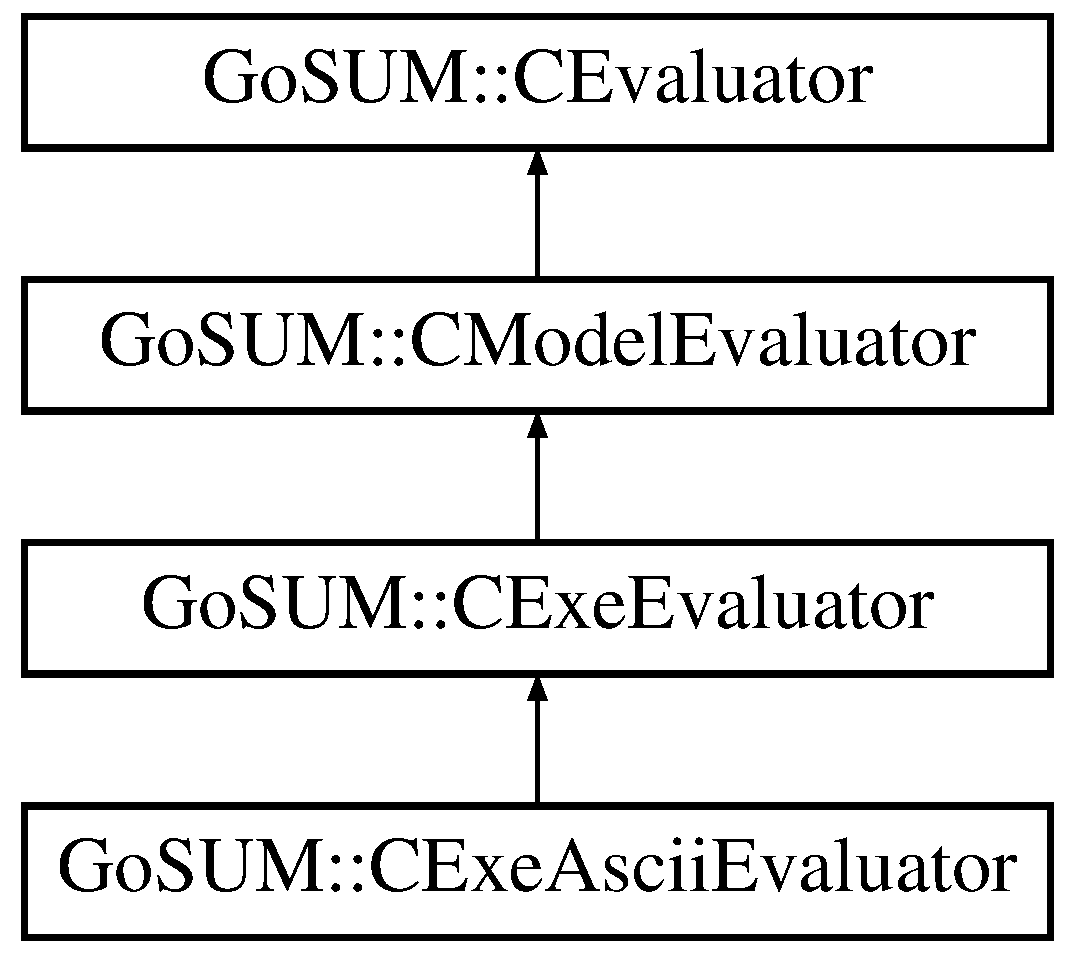
\includegraphics[height=4.000000cm]{class_go_s_u_m_1_1_c_exe_ascii_evaluator}
\end{center}
\end{figure}
\subsection*{Public Member Functions}
\begin{DoxyCompactItemize}
\item 
\hyperlink{class_go_s_u_m_1_1_c_exe_ascii_evaluator_aaf0d92f18ef702c15efd603d172ff1b9}{C\-Exe\-Ascii\-Evaluator} ()
\item 
\hyperlink{class_go_s_u_m_1_1_c_exe_ascii_evaluator_aeb20b18053aef9a95d6d3ecc15b11779}{C\-Exe\-Ascii\-Evaluator} (const \hyperlink{class_go_s_u_m_1_1_c_input_parameters}{C\-Input\-Parameters} $\ast$\-\_\-p\-I\-P, \hyperlink{class_go_s_u_m_1_1_c_output_states}{C\-Output\-States} $\ast$\-\_\-p\-O\-S, int \-\_\-trd\-I)
\item 
virtual \hyperlink{class_go_s_u_m_1_1_c_exe_ascii_evaluator_ac6292f4ae77f94e328d1ee2c16150378}{$\sim$\-C\-Exe\-Ascii\-Evaluator} ()
\end{DoxyCompactItemize}
\subsection*{Protected Member Functions}
\begin{DoxyCompactItemize}
\item 
{\footnotesize template$<$class Archive $>$ }\\void \hyperlink{class_go_s_u_m_1_1_c_exe_ascii_evaluator_a68297034ace4c45caa7a1dcd5ff022de}{serialize} (Archive \&ar, const unsigned int version)
\item 
virtual void \hyperlink{class_go_s_u_m_1_1_c_exe_ascii_evaluator_a4044398bdc3cae949e94786e37d0f477}{write\-To} (std\-::string \-\_\-fname, const Array\-Xd \&\-\_\-\-X, std\-::string \-\_\-\-Xname)
\item 
virtual void \hyperlink{class_go_s_u_m_1_1_c_exe_ascii_evaluator_a6bc1881693432b58ece64fa77eabd444}{read\-From} (std\-::string \-\_\-fname, Array\-Xd \&\-\_\-\-Y, std\-::string \-\_\-\-Yname)
\item 
virtual int \hyperlink{class_go_s_u_m_1_1_c_exe_ascii_evaluator_a5447eaef9e5a45f711de007b71fa4e0c}{read\-Size\-From} (std\-::string \-\_\-fname, std\-::string \-\_\-\-Yname)
\end{DoxyCompactItemize}
\subsection*{Friends}
\begin{DoxyCompactItemize}
\item 
class \hyperlink{class_go_s_u_m_1_1_c_exe_ascii_evaluator_ac98d07dd8f7b70e16ccb9a01abf56b9c}{boost\-::serialization\-::access}
\begin{DoxyCompactList}\small\item\em Boost serialization. \end{DoxyCompactList}\end{DoxyCompactItemize}
\subsection*{Additional Inherited Members}


\subsection{Detailed Description}
Class for the evaluator with ascii i/o and .exe. 

\subsection{Constructor \& Destructor Documentation}
\hypertarget{class_go_s_u_m_1_1_c_exe_ascii_evaluator_aaf0d92f18ef702c15efd603d172ff1b9}{\index{Go\-S\-U\-M\-::\-C\-Exe\-Ascii\-Evaluator@{Go\-S\-U\-M\-::\-C\-Exe\-Ascii\-Evaluator}!C\-Exe\-Ascii\-Evaluator@{C\-Exe\-Ascii\-Evaluator}}
\index{C\-Exe\-Ascii\-Evaluator@{C\-Exe\-Ascii\-Evaluator}!GoSUM::CExeAsciiEvaluator@{Go\-S\-U\-M\-::\-C\-Exe\-Ascii\-Evaluator}}
\subsubsection[{C\-Exe\-Ascii\-Evaluator}]{\setlength{\rightskip}{0pt plus 5cm}Go\-S\-U\-M\-::\-C\-Exe\-Ascii\-Evaluator\-::\-C\-Exe\-Ascii\-Evaluator (
\begin{DoxyParamCaption}
{}
\end{DoxyParamCaption}
)\hspace{0.3cm}{\ttfamily [inline]}}}\label{class_go_s_u_m_1_1_c_exe_ascii_evaluator_aaf0d92f18ef702c15efd603d172ff1b9}
\hypertarget{class_go_s_u_m_1_1_c_exe_ascii_evaluator_aeb20b18053aef9a95d6d3ecc15b11779}{\index{Go\-S\-U\-M\-::\-C\-Exe\-Ascii\-Evaluator@{Go\-S\-U\-M\-::\-C\-Exe\-Ascii\-Evaluator}!C\-Exe\-Ascii\-Evaluator@{C\-Exe\-Ascii\-Evaluator}}
\index{C\-Exe\-Ascii\-Evaluator@{C\-Exe\-Ascii\-Evaluator}!GoSUM::CExeAsciiEvaluator@{Go\-S\-U\-M\-::\-C\-Exe\-Ascii\-Evaluator}}
\subsubsection[{C\-Exe\-Ascii\-Evaluator}]{\setlength{\rightskip}{0pt plus 5cm}Go\-S\-U\-M\-::\-C\-Exe\-Ascii\-Evaluator\-::\-C\-Exe\-Ascii\-Evaluator (
\begin{DoxyParamCaption}
\item[{const {\bf C\-Input\-Parameters} $\ast$}]{\-\_\-p\-I\-P, }
\item[{{\bf C\-Output\-States} $\ast$}]{\-\_\-p\-O\-S, }
\item[{int}]{\-\_\-trd\-I}
\end{DoxyParamCaption}
)\hspace{0.3cm}{\ttfamily [inline]}}}\label{class_go_s_u_m_1_1_c_exe_ascii_evaluator_aeb20b18053aef9a95d6d3ecc15b11779}
\hypertarget{class_go_s_u_m_1_1_c_exe_ascii_evaluator_ac6292f4ae77f94e328d1ee2c16150378}{\index{Go\-S\-U\-M\-::\-C\-Exe\-Ascii\-Evaluator@{Go\-S\-U\-M\-::\-C\-Exe\-Ascii\-Evaluator}!$\sim$\-C\-Exe\-Ascii\-Evaluator@{$\sim$\-C\-Exe\-Ascii\-Evaluator}}
\index{$\sim$\-C\-Exe\-Ascii\-Evaluator@{$\sim$\-C\-Exe\-Ascii\-Evaluator}!GoSUM::CExeAsciiEvaluator@{Go\-S\-U\-M\-::\-C\-Exe\-Ascii\-Evaluator}}
\subsubsection[{$\sim$\-C\-Exe\-Ascii\-Evaluator}]{\setlength{\rightskip}{0pt plus 5cm}virtual Go\-S\-U\-M\-::\-C\-Exe\-Ascii\-Evaluator\-::$\sim$\-C\-Exe\-Ascii\-Evaluator (
\begin{DoxyParamCaption}
{}
\end{DoxyParamCaption}
)\hspace{0.3cm}{\ttfamily [inline]}, {\ttfamily [virtual]}}}\label{class_go_s_u_m_1_1_c_exe_ascii_evaluator_ac6292f4ae77f94e328d1ee2c16150378}


\subsection{Member Function Documentation}
\hypertarget{class_go_s_u_m_1_1_c_exe_ascii_evaluator_a6bc1881693432b58ece64fa77eabd444}{\index{Go\-S\-U\-M\-::\-C\-Exe\-Ascii\-Evaluator@{Go\-S\-U\-M\-::\-C\-Exe\-Ascii\-Evaluator}!read\-From@{read\-From}}
\index{read\-From@{read\-From}!GoSUM::CExeAsciiEvaluator@{Go\-S\-U\-M\-::\-C\-Exe\-Ascii\-Evaluator}}
\subsubsection[{read\-From}]{\setlength{\rightskip}{0pt plus 5cm}void Go\-S\-U\-M\-::\-C\-Exe\-Ascii\-Evaluator\-::read\-From (
\begin{DoxyParamCaption}
\item[{std\-::string}]{\-\_\-fname, }
\item[{Array\-Xd \&}]{\-\_\-\-Y, }
\item[{std\-::string}]{\-\_\-\-Yname}
\end{DoxyParamCaption}
)\hspace{0.3cm}{\ttfamily [protected]}, {\ttfamily [virtual]}}}\label{class_go_s_u_m_1_1_c_exe_ascii_evaluator_a6bc1881693432b58ece64fa77eabd444}


Implements \hyperlink{class_go_s_u_m_1_1_c_exe_evaluator_af453aa942a20e6494a4cd7685ace1948}{Go\-S\-U\-M\-::\-C\-Exe\-Evaluator}.

\hypertarget{class_go_s_u_m_1_1_c_exe_ascii_evaluator_a5447eaef9e5a45f711de007b71fa4e0c}{\index{Go\-S\-U\-M\-::\-C\-Exe\-Ascii\-Evaluator@{Go\-S\-U\-M\-::\-C\-Exe\-Ascii\-Evaluator}!read\-Size\-From@{read\-Size\-From}}
\index{read\-Size\-From@{read\-Size\-From}!GoSUM::CExeAsciiEvaluator@{Go\-S\-U\-M\-::\-C\-Exe\-Ascii\-Evaluator}}
\subsubsection[{read\-Size\-From}]{\setlength{\rightskip}{0pt plus 5cm}int Go\-S\-U\-M\-::\-C\-Exe\-Ascii\-Evaluator\-::read\-Size\-From (
\begin{DoxyParamCaption}
\item[{std\-::string}]{\-\_\-fname, }
\item[{std\-::string}]{\-\_\-\-Yname}
\end{DoxyParamCaption}
)\hspace{0.3cm}{\ttfamily [protected]}, {\ttfamily [virtual]}}}\label{class_go_s_u_m_1_1_c_exe_ascii_evaluator_a5447eaef9e5a45f711de007b71fa4e0c}


Implements \hyperlink{class_go_s_u_m_1_1_c_exe_evaluator_a1f7820ae9bd4795547dca1611769a182}{Go\-S\-U\-M\-::\-C\-Exe\-Evaluator}.

\hypertarget{class_go_s_u_m_1_1_c_exe_ascii_evaluator_a68297034ace4c45caa7a1dcd5ff022de}{\index{Go\-S\-U\-M\-::\-C\-Exe\-Ascii\-Evaluator@{Go\-S\-U\-M\-::\-C\-Exe\-Ascii\-Evaluator}!serialize@{serialize}}
\index{serialize@{serialize}!GoSUM::CExeAsciiEvaluator@{Go\-S\-U\-M\-::\-C\-Exe\-Ascii\-Evaluator}}
\subsubsection[{serialize}]{\setlength{\rightskip}{0pt plus 5cm}template$<$class Archive $>$ void Go\-S\-U\-M\-::\-C\-Exe\-Ascii\-Evaluator\-::serialize (
\begin{DoxyParamCaption}
\item[{Archive \&}]{ar, }
\item[{const unsigned int}]{version}
\end{DoxyParamCaption}
)\hspace{0.3cm}{\ttfamily [protected]}}}\label{class_go_s_u_m_1_1_c_exe_ascii_evaluator_a68297034ace4c45caa7a1dcd5ff022de}


Reimplemented from \hyperlink{class_go_s_u_m_1_1_c_exe_evaluator_adccb3c9acae9f916d8be1a9720d5bcc1}{Go\-S\-U\-M\-::\-C\-Exe\-Evaluator}.

\hypertarget{class_go_s_u_m_1_1_c_exe_ascii_evaluator_a4044398bdc3cae949e94786e37d0f477}{\index{Go\-S\-U\-M\-::\-C\-Exe\-Ascii\-Evaluator@{Go\-S\-U\-M\-::\-C\-Exe\-Ascii\-Evaluator}!write\-To@{write\-To}}
\index{write\-To@{write\-To}!GoSUM::CExeAsciiEvaluator@{Go\-S\-U\-M\-::\-C\-Exe\-Ascii\-Evaluator}}
\subsubsection[{write\-To}]{\setlength{\rightskip}{0pt plus 5cm}void Go\-S\-U\-M\-::\-C\-Exe\-Ascii\-Evaluator\-::write\-To (
\begin{DoxyParamCaption}
\item[{std\-::string}]{\-\_\-fname, }
\item[{const Array\-Xd \&}]{\-\_\-\-X, }
\item[{std\-::string}]{\-\_\-\-Xname}
\end{DoxyParamCaption}
)\hspace{0.3cm}{\ttfamily [protected]}, {\ttfamily [virtual]}}}\label{class_go_s_u_m_1_1_c_exe_ascii_evaluator_a4044398bdc3cae949e94786e37d0f477}


Implements \hyperlink{class_go_s_u_m_1_1_c_exe_evaluator_acb14cd0bed268c9f34a0fef4f9d8deb6}{Go\-S\-U\-M\-::\-C\-Exe\-Evaluator}.



\subsection{Friends And Related Function Documentation}
\hypertarget{class_go_s_u_m_1_1_c_exe_ascii_evaluator_ac98d07dd8f7b70e16ccb9a01abf56b9c}{\index{Go\-S\-U\-M\-::\-C\-Exe\-Ascii\-Evaluator@{Go\-S\-U\-M\-::\-C\-Exe\-Ascii\-Evaluator}!boost\-::serialization\-::access@{boost\-::serialization\-::access}}
\index{boost\-::serialization\-::access@{boost\-::serialization\-::access}!GoSUM::CExeAsciiEvaluator@{Go\-S\-U\-M\-::\-C\-Exe\-Ascii\-Evaluator}}
\subsubsection[{boost\-::serialization\-::access}]{\setlength{\rightskip}{0pt plus 5cm}friend class boost\-::serialization\-::access\hspace{0.3cm}{\ttfamily [friend]}}}\label{class_go_s_u_m_1_1_c_exe_ascii_evaluator_ac98d07dd8f7b70e16ccb9a01abf56b9c}


Boost serialization. 



The documentation for this class was generated from the following files\-:\begin{DoxyCompactItemize}
\item 
C\-:/\-Development/core/\hyperlink{_original_model_8h}{Original\-Model.\-h}\item 
C\-:/\-Development/core/\hyperlink{_original_model_8cpp}{Original\-Model.\-cpp}\end{DoxyCompactItemize}

\hypertarget{class_go_s_u_m_1_1_c_exe_evaluator}{\section{Go\-S\-U\-M\-:\-:C\-Exe\-Evaluator Class Reference}
\label{class_go_s_u_m_1_1_c_exe_evaluator}\index{Go\-S\-U\-M\-::\-C\-Exe\-Evaluator@{Go\-S\-U\-M\-::\-C\-Exe\-Evaluator}}
}


Template for the evaluator with some file i/o and .exe derived from \hyperlink{class_go_s_u_m_1_1_c_model_evaluator}{C\-Model\-Evaluator}.  




{\ttfamily \#include $<$Original\-Model.\-h$>$}

Inheritance diagram for Go\-S\-U\-M\-:\-:C\-Exe\-Evaluator\-:\begin{figure}[H]
\begin{center}
\leavevmode
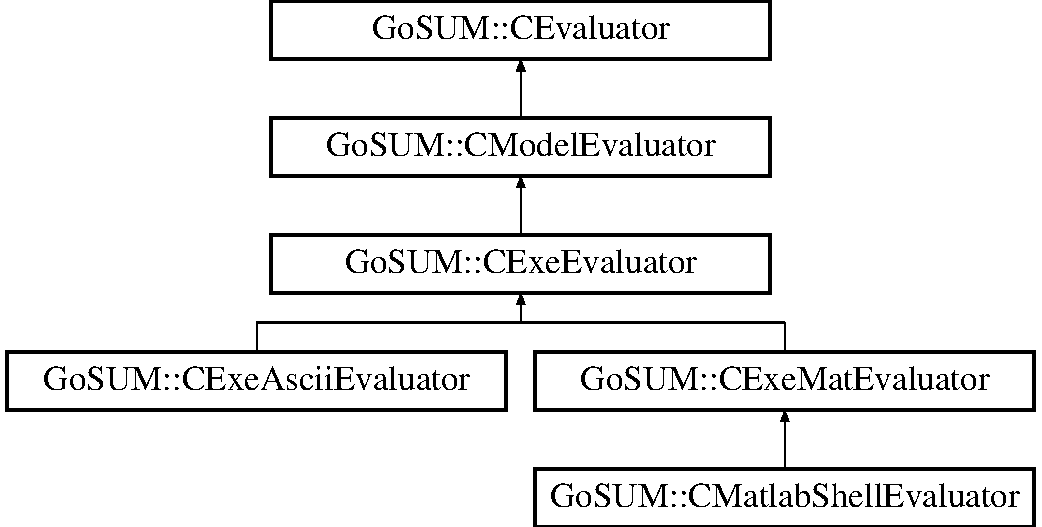
\includegraphics[height=5.000000cm]{class_go_s_u_m_1_1_c_exe_evaluator}
\end{center}
\end{figure}
\subsection*{Public Member Functions}
\begin{DoxyCompactItemize}
\item 
\hyperlink{class_go_s_u_m_1_1_c_exe_evaluator_a35eb03f3e1189c969a81c57b6fe73b92}{C\-Exe\-Evaluator} ()
\item 
\hyperlink{class_go_s_u_m_1_1_c_exe_evaluator_af3721a6b87e61dcdb5e79092c1455fa7}{C\-Exe\-Evaluator} (const \hyperlink{class_go_s_u_m_1_1_c_input_parameters}{C\-Input\-Parameters} $\ast$\-\_\-p\-I\-P, \hyperlink{class_go_s_u_m_1_1_c_output_states}{C\-Output\-States} $\ast$\-\_\-p\-O\-S, int \-\_\-trd\-I)
\item 
virtual \hyperlink{class_go_s_u_m_1_1_c_exe_evaluator_ad6c59f01d0d1759eadb90d7f577ed8e0}{$\sim$\-C\-Exe\-Evaluator} ()
\item 
virtual void \hyperlink{class_go_s_u_m_1_1_c_exe_evaluator_abdc5b11c31ed73a34499e135eab45ef8}{open\-Evaluation} ()
\begin{DoxyCompactList}\small\item\em Opens, i.\-e. prepares evaluation process. \end{DoxyCompactList}\item 
virtual Array\-Xd \hyperlink{class_go_s_u_m_1_1_c_exe_evaluator_ae388d8a8bef01f0a3fc3e6cecb341576}{operator()} (const Array\-Xd \&X)
\begin{DoxyCompactList}\small\item\em Returns output state evaluated on for a single input parameter n-\/tuple. \end{DoxyCompactList}\item 
virtual int \hyperlink{class_go_s_u_m_1_1_c_exe_evaluator_a3a8ea5f4af5c653421f27ace8fb57181}{evaluate\-Outputs\-Size} ()
\begin{DoxyCompactList}\small\item\em Evaluates outputs size by running model evaluator. \end{DoxyCompactList}\item 
virtual void \hyperlink{class_go_s_u_m_1_1_c_exe_evaluator_a0e18062b8ec197437febdfa46dd7b45b}{close\-Evaluation} ()
\begin{DoxyCompactList}\small\item\em Closes evaluation process. \end{DoxyCompactList}\end{DoxyCompactItemize}
\subsection*{Protected Member Functions}
\begin{DoxyCompactItemize}
\item 
{\footnotesize template$<$class Archive $>$ }\\void \hyperlink{class_go_s_u_m_1_1_c_exe_evaluator_adccb3c9acae9f916d8be1a9720d5bcc1}{serialize} (Archive \&ar, const unsigned int version)
\item 
virtual void \hyperlink{class_go_s_u_m_1_1_c_exe_evaluator_aeb6c371d09cbc3cb3a0152779a32bf52}{system\-Command} (std\-::ostringstream \&cmd)
\item 
virtual void \hyperlink{class_go_s_u_m_1_1_c_exe_evaluator_acb14cd0bed268c9f34a0fef4f9d8deb6}{write\-To} (std\-::string \-\_\-fname, const Array\-Xd \&\-\_\-\-X, std\-::string \-\_\-\-Xname)=0
\item 
virtual void \hyperlink{class_go_s_u_m_1_1_c_exe_evaluator_af453aa942a20e6494a4cd7685ace1948}{read\-From} (std\-::string \-\_\-fname, Array\-Xd \&\-\_\-\-Y, std\-::string \-\_\-\-Yname)=0
\item 
virtual int \hyperlink{class_go_s_u_m_1_1_c_exe_evaluator_a1f7820ae9bd4795547dca1611769a182}{read\-Size\-From} (std\-::string \-\_\-fname, std\-::string \-\_\-\-Yname)=0
\end{DoxyCompactItemize}
\subsection*{Protected Attributes}
\begin{DoxyCompactItemize}
\item 
Q\-Process $\ast$ \hyperlink{class_go_s_u_m_1_1_c_exe_evaluator_a92e5435e10a507cdc893eec96f7dfae0}{p\-P}
\begin{DoxyCompactList}\small\item\em Points to the qprocess. \end{DoxyCompactList}\end{DoxyCompactItemize}
\subsection*{Friends}
\begin{DoxyCompactItemize}
\item 
class \hyperlink{class_go_s_u_m_1_1_c_exe_evaluator_ac98d07dd8f7b70e16ccb9a01abf56b9c}{boost\-::serialization\-::access}
\begin{DoxyCompactList}\small\item\em Boost serialization. \end{DoxyCompactList}\end{DoxyCompactItemize}
\subsection*{Additional Inherited Members}


\subsection{Detailed Description}
Template for the evaluator with some file i/o and .exe derived from \hyperlink{class_go_s_u_m_1_1_c_model_evaluator}{C\-Model\-Evaluator}. 

\subsection{Constructor \& Destructor Documentation}
\hypertarget{class_go_s_u_m_1_1_c_exe_evaluator_a35eb03f3e1189c969a81c57b6fe73b92}{\index{Go\-S\-U\-M\-::\-C\-Exe\-Evaluator@{Go\-S\-U\-M\-::\-C\-Exe\-Evaluator}!C\-Exe\-Evaluator@{C\-Exe\-Evaluator}}
\index{C\-Exe\-Evaluator@{C\-Exe\-Evaluator}!GoSUM::CExeEvaluator@{Go\-S\-U\-M\-::\-C\-Exe\-Evaluator}}
\subsubsection[{C\-Exe\-Evaluator}]{\setlength{\rightskip}{0pt plus 5cm}Go\-S\-U\-M\-::\-C\-Exe\-Evaluator\-::\-C\-Exe\-Evaluator (
\begin{DoxyParamCaption}
{}
\end{DoxyParamCaption}
)\hspace{0.3cm}{\ttfamily [inline]}}}\label{class_go_s_u_m_1_1_c_exe_evaluator_a35eb03f3e1189c969a81c57b6fe73b92}
\hypertarget{class_go_s_u_m_1_1_c_exe_evaluator_af3721a6b87e61dcdb5e79092c1455fa7}{\index{Go\-S\-U\-M\-::\-C\-Exe\-Evaluator@{Go\-S\-U\-M\-::\-C\-Exe\-Evaluator}!C\-Exe\-Evaluator@{C\-Exe\-Evaluator}}
\index{C\-Exe\-Evaluator@{C\-Exe\-Evaluator}!GoSUM::CExeEvaluator@{Go\-S\-U\-M\-::\-C\-Exe\-Evaluator}}
\subsubsection[{C\-Exe\-Evaluator}]{\setlength{\rightskip}{0pt plus 5cm}Go\-S\-U\-M\-::\-C\-Exe\-Evaluator\-::\-C\-Exe\-Evaluator (
\begin{DoxyParamCaption}
\item[{const {\bf C\-Input\-Parameters} $\ast$}]{\-\_\-p\-I\-P, }
\item[{{\bf C\-Output\-States} $\ast$}]{\-\_\-p\-O\-S, }
\item[{int}]{\-\_\-trd\-I}
\end{DoxyParamCaption}
)\hspace{0.3cm}{\ttfamily [inline]}}}\label{class_go_s_u_m_1_1_c_exe_evaluator_af3721a6b87e61dcdb5e79092c1455fa7}
\hypertarget{class_go_s_u_m_1_1_c_exe_evaluator_ad6c59f01d0d1759eadb90d7f577ed8e0}{\index{Go\-S\-U\-M\-::\-C\-Exe\-Evaluator@{Go\-S\-U\-M\-::\-C\-Exe\-Evaluator}!$\sim$\-C\-Exe\-Evaluator@{$\sim$\-C\-Exe\-Evaluator}}
\index{$\sim$\-C\-Exe\-Evaluator@{$\sim$\-C\-Exe\-Evaluator}!GoSUM::CExeEvaluator@{Go\-S\-U\-M\-::\-C\-Exe\-Evaluator}}
\subsubsection[{$\sim$\-C\-Exe\-Evaluator}]{\setlength{\rightskip}{0pt plus 5cm}virtual Go\-S\-U\-M\-::\-C\-Exe\-Evaluator\-::$\sim$\-C\-Exe\-Evaluator (
\begin{DoxyParamCaption}
{}
\end{DoxyParamCaption}
)\hspace{0.3cm}{\ttfamily [inline]}, {\ttfamily [virtual]}}}\label{class_go_s_u_m_1_1_c_exe_evaluator_ad6c59f01d0d1759eadb90d7f577ed8e0}


\subsection{Member Function Documentation}
\hypertarget{class_go_s_u_m_1_1_c_exe_evaluator_a0e18062b8ec197437febdfa46dd7b45b}{\index{Go\-S\-U\-M\-::\-C\-Exe\-Evaluator@{Go\-S\-U\-M\-::\-C\-Exe\-Evaluator}!close\-Evaluation@{close\-Evaluation}}
\index{close\-Evaluation@{close\-Evaluation}!GoSUM::CExeEvaluator@{Go\-S\-U\-M\-::\-C\-Exe\-Evaluator}}
\subsubsection[{close\-Evaluation}]{\setlength{\rightskip}{0pt plus 5cm}void Go\-S\-U\-M\-::\-C\-Exe\-Evaluator\-::close\-Evaluation (
\begin{DoxyParamCaption}
{}
\end{DoxyParamCaption}
)\hspace{0.3cm}{\ttfamily [virtual]}}}\label{class_go_s_u_m_1_1_c_exe_evaluator_a0e18062b8ec197437febdfa46dd7b45b}


Closes evaluation process. 



Implements \hyperlink{class_go_s_u_m_1_1_c_model_evaluator_a7ed9761e18560616881ebe459c6b8952}{Go\-S\-U\-M\-::\-C\-Model\-Evaluator}.

\hypertarget{class_go_s_u_m_1_1_c_exe_evaluator_a3a8ea5f4af5c653421f27ace8fb57181}{\index{Go\-S\-U\-M\-::\-C\-Exe\-Evaluator@{Go\-S\-U\-M\-::\-C\-Exe\-Evaluator}!evaluate\-Outputs\-Size@{evaluate\-Outputs\-Size}}
\index{evaluate\-Outputs\-Size@{evaluate\-Outputs\-Size}!GoSUM::CExeEvaluator@{Go\-S\-U\-M\-::\-C\-Exe\-Evaluator}}
\subsubsection[{evaluate\-Outputs\-Size}]{\setlength{\rightskip}{0pt plus 5cm}int Go\-S\-U\-M\-::\-C\-Exe\-Evaluator\-::evaluate\-Outputs\-Size (
\begin{DoxyParamCaption}
{}
\end{DoxyParamCaption}
)\hspace{0.3cm}{\ttfamily [virtual]}}}\label{class_go_s_u_m_1_1_c_exe_evaluator_a3a8ea5f4af5c653421f27ace8fb57181}


Evaluates outputs size by running model evaluator. 



Reimplemented from \hyperlink{class_go_s_u_m_1_1_c_model_evaluator_a822314faa443612c8840e6252018efb2}{Go\-S\-U\-M\-::\-C\-Model\-Evaluator}.

\hypertarget{class_go_s_u_m_1_1_c_exe_evaluator_abdc5b11c31ed73a34499e135eab45ef8}{\index{Go\-S\-U\-M\-::\-C\-Exe\-Evaluator@{Go\-S\-U\-M\-::\-C\-Exe\-Evaluator}!open\-Evaluation@{open\-Evaluation}}
\index{open\-Evaluation@{open\-Evaluation}!GoSUM::CExeEvaluator@{Go\-S\-U\-M\-::\-C\-Exe\-Evaluator}}
\subsubsection[{open\-Evaluation}]{\setlength{\rightskip}{0pt plus 5cm}void Go\-S\-U\-M\-::\-C\-Exe\-Evaluator\-::open\-Evaluation (
\begin{DoxyParamCaption}
{}
\end{DoxyParamCaption}
)\hspace{0.3cm}{\ttfamily [virtual]}}}\label{class_go_s_u_m_1_1_c_exe_evaluator_abdc5b11c31ed73a34499e135eab45ef8}


Opens, i.\-e. prepares evaluation process. 



Implements \hyperlink{class_go_s_u_m_1_1_c_model_evaluator_a0f5afddb7ed75aad687d3a00e44012a0}{Go\-S\-U\-M\-::\-C\-Model\-Evaluator}.

\hypertarget{class_go_s_u_m_1_1_c_exe_evaluator_ae388d8a8bef01f0a3fc3e6cecb341576}{\index{Go\-S\-U\-M\-::\-C\-Exe\-Evaluator@{Go\-S\-U\-M\-::\-C\-Exe\-Evaluator}!operator()@{operator()}}
\index{operator()@{operator()}!GoSUM::CExeEvaluator@{Go\-S\-U\-M\-::\-C\-Exe\-Evaluator}}
\subsubsection[{operator()}]{\setlength{\rightskip}{0pt plus 5cm}Array\-Xd Go\-S\-U\-M\-::\-C\-Exe\-Evaluator\-::operator() (
\begin{DoxyParamCaption}
\item[{const Array\-Xd \&}]{X}
\end{DoxyParamCaption}
)\hspace{0.3cm}{\ttfamily [virtual]}}}\label{class_go_s_u_m_1_1_c_exe_evaluator_ae388d8a8bef01f0a3fc3e6cecb341576}


Returns output state evaluated on for a single input parameter n-\/tuple. 



Implements \hyperlink{class_go_s_u_m_1_1_c_model_evaluator_a17541eada67797802edcae14533361ad}{Go\-S\-U\-M\-::\-C\-Model\-Evaluator}.

\hypertarget{class_go_s_u_m_1_1_c_exe_evaluator_af453aa942a20e6494a4cd7685ace1948}{\index{Go\-S\-U\-M\-::\-C\-Exe\-Evaluator@{Go\-S\-U\-M\-::\-C\-Exe\-Evaluator}!read\-From@{read\-From}}
\index{read\-From@{read\-From}!GoSUM::CExeEvaluator@{Go\-S\-U\-M\-::\-C\-Exe\-Evaluator}}
\subsubsection[{read\-From}]{\setlength{\rightskip}{0pt plus 5cm}virtual void Go\-S\-U\-M\-::\-C\-Exe\-Evaluator\-::read\-From (
\begin{DoxyParamCaption}
\item[{std\-::string}]{\-\_\-fname, }
\item[{Array\-Xd \&}]{\-\_\-\-Y, }
\item[{std\-::string}]{\-\_\-\-Yname}
\end{DoxyParamCaption}
)\hspace{0.3cm}{\ttfamily [protected]}, {\ttfamily [pure virtual]}}}\label{class_go_s_u_m_1_1_c_exe_evaluator_af453aa942a20e6494a4cd7685ace1948}


Implemented in \hyperlink{class_go_s_u_m_1_1_c_exe_mat_evaluator_ac47387e84bc69c1e39fbe43b15465473}{Go\-S\-U\-M\-::\-C\-Exe\-Mat\-Evaluator}, and \hyperlink{class_go_s_u_m_1_1_c_exe_ascii_evaluator_a6bc1881693432b58ece64fa77eabd444}{Go\-S\-U\-M\-::\-C\-Exe\-Ascii\-Evaluator}.

\hypertarget{class_go_s_u_m_1_1_c_exe_evaluator_a1f7820ae9bd4795547dca1611769a182}{\index{Go\-S\-U\-M\-::\-C\-Exe\-Evaluator@{Go\-S\-U\-M\-::\-C\-Exe\-Evaluator}!read\-Size\-From@{read\-Size\-From}}
\index{read\-Size\-From@{read\-Size\-From}!GoSUM::CExeEvaluator@{Go\-S\-U\-M\-::\-C\-Exe\-Evaluator}}
\subsubsection[{read\-Size\-From}]{\setlength{\rightskip}{0pt plus 5cm}virtual int Go\-S\-U\-M\-::\-C\-Exe\-Evaluator\-::read\-Size\-From (
\begin{DoxyParamCaption}
\item[{std\-::string}]{\-\_\-fname, }
\item[{std\-::string}]{\-\_\-\-Yname}
\end{DoxyParamCaption}
)\hspace{0.3cm}{\ttfamily [protected]}, {\ttfamily [pure virtual]}}}\label{class_go_s_u_m_1_1_c_exe_evaluator_a1f7820ae9bd4795547dca1611769a182}


Implemented in \hyperlink{class_go_s_u_m_1_1_c_exe_mat_evaluator_a84e80ccc1d62a41f3d7881e125bee446}{Go\-S\-U\-M\-::\-C\-Exe\-Mat\-Evaluator}, and \hyperlink{class_go_s_u_m_1_1_c_exe_ascii_evaluator_a5447eaef9e5a45f711de007b71fa4e0c}{Go\-S\-U\-M\-::\-C\-Exe\-Ascii\-Evaluator}.

\hypertarget{class_go_s_u_m_1_1_c_exe_evaluator_adccb3c9acae9f916d8be1a9720d5bcc1}{\index{Go\-S\-U\-M\-::\-C\-Exe\-Evaluator@{Go\-S\-U\-M\-::\-C\-Exe\-Evaluator}!serialize@{serialize}}
\index{serialize@{serialize}!GoSUM::CExeEvaluator@{Go\-S\-U\-M\-::\-C\-Exe\-Evaluator}}
\subsubsection[{serialize}]{\setlength{\rightskip}{0pt plus 5cm}template$<$class Archive $>$ void Go\-S\-U\-M\-::\-C\-Exe\-Evaluator\-::serialize (
\begin{DoxyParamCaption}
\item[{Archive \&}]{ar, }
\item[{const unsigned int}]{version}
\end{DoxyParamCaption}
)\hspace{0.3cm}{\ttfamily [protected]}}}\label{class_go_s_u_m_1_1_c_exe_evaluator_adccb3c9acae9f916d8be1a9720d5bcc1}


Reimplemented from \hyperlink{class_go_s_u_m_1_1_c_model_evaluator_a80e334f1496f3bee1da84cee050a72a1}{Go\-S\-U\-M\-::\-C\-Model\-Evaluator}.



Reimplemented in \hyperlink{class_go_s_u_m_1_1_c_matlab_shell_evaluator_af84e659441da0694bff64c2d955831b9}{Go\-S\-U\-M\-::\-C\-Matlab\-Shell\-Evaluator}, \hyperlink{class_go_s_u_m_1_1_c_exe_mat_evaluator_a2e5121b751aaeb6f5c805cfe0312c20d}{Go\-S\-U\-M\-::\-C\-Exe\-Mat\-Evaluator}, and \hyperlink{class_go_s_u_m_1_1_c_exe_ascii_evaluator_a68297034ace4c45caa7a1dcd5ff022de}{Go\-S\-U\-M\-::\-C\-Exe\-Ascii\-Evaluator}.

\hypertarget{class_go_s_u_m_1_1_c_exe_evaluator_aeb6c371d09cbc3cb3a0152779a32bf52}{\index{Go\-S\-U\-M\-::\-C\-Exe\-Evaluator@{Go\-S\-U\-M\-::\-C\-Exe\-Evaluator}!system\-Command@{system\-Command}}
\index{system\-Command@{system\-Command}!GoSUM::CExeEvaluator@{Go\-S\-U\-M\-::\-C\-Exe\-Evaluator}}
\subsubsection[{system\-Command}]{\setlength{\rightskip}{0pt plus 5cm}virtual void Go\-S\-U\-M\-::\-C\-Exe\-Evaluator\-::system\-Command (
\begin{DoxyParamCaption}
\item[{std\-::ostringstream \&}]{cmd}
\end{DoxyParamCaption}
)\hspace{0.3cm}{\ttfamily [inline]}, {\ttfamily [protected]}, {\ttfamily [virtual]}}}\label{class_go_s_u_m_1_1_c_exe_evaluator_aeb6c371d09cbc3cb3a0152779a32bf52}


Reimplemented in \hyperlink{class_go_s_u_m_1_1_c_matlab_shell_evaluator_ab365048eef74e7b837fcb4420f763f1f}{Go\-S\-U\-M\-::\-C\-Matlab\-Shell\-Evaluator}.

\hypertarget{class_go_s_u_m_1_1_c_exe_evaluator_acb14cd0bed268c9f34a0fef4f9d8deb6}{\index{Go\-S\-U\-M\-::\-C\-Exe\-Evaluator@{Go\-S\-U\-M\-::\-C\-Exe\-Evaluator}!write\-To@{write\-To}}
\index{write\-To@{write\-To}!GoSUM::CExeEvaluator@{Go\-S\-U\-M\-::\-C\-Exe\-Evaluator}}
\subsubsection[{write\-To}]{\setlength{\rightskip}{0pt plus 5cm}virtual void Go\-S\-U\-M\-::\-C\-Exe\-Evaluator\-::write\-To (
\begin{DoxyParamCaption}
\item[{std\-::string}]{\-\_\-fname, }
\item[{const Array\-Xd \&}]{\-\_\-\-X, }
\item[{std\-::string}]{\-\_\-\-Xname}
\end{DoxyParamCaption}
)\hspace{0.3cm}{\ttfamily [protected]}, {\ttfamily [pure virtual]}}}\label{class_go_s_u_m_1_1_c_exe_evaluator_acb14cd0bed268c9f34a0fef4f9d8deb6}


Implemented in \hyperlink{class_go_s_u_m_1_1_c_exe_mat_evaluator_abf90e8ece5e782c8a60cbd0021e3dfa1}{Go\-S\-U\-M\-::\-C\-Exe\-Mat\-Evaluator}, and \hyperlink{class_go_s_u_m_1_1_c_exe_ascii_evaluator_a4044398bdc3cae949e94786e37d0f477}{Go\-S\-U\-M\-::\-C\-Exe\-Ascii\-Evaluator}.



\subsection{Friends And Related Function Documentation}
\hypertarget{class_go_s_u_m_1_1_c_exe_evaluator_ac98d07dd8f7b70e16ccb9a01abf56b9c}{\index{Go\-S\-U\-M\-::\-C\-Exe\-Evaluator@{Go\-S\-U\-M\-::\-C\-Exe\-Evaluator}!boost\-::serialization\-::access@{boost\-::serialization\-::access}}
\index{boost\-::serialization\-::access@{boost\-::serialization\-::access}!GoSUM::CExeEvaluator@{Go\-S\-U\-M\-::\-C\-Exe\-Evaluator}}
\subsubsection[{boost\-::serialization\-::access}]{\setlength{\rightskip}{0pt plus 5cm}friend class boost\-::serialization\-::access\hspace{0.3cm}{\ttfamily [friend]}}}\label{class_go_s_u_m_1_1_c_exe_evaluator_ac98d07dd8f7b70e16ccb9a01abf56b9c}


Boost serialization. 



\subsection{Member Data Documentation}
\hypertarget{class_go_s_u_m_1_1_c_exe_evaluator_a92e5435e10a507cdc893eec96f7dfae0}{\index{Go\-S\-U\-M\-::\-C\-Exe\-Evaluator@{Go\-S\-U\-M\-::\-C\-Exe\-Evaluator}!p\-P@{p\-P}}
\index{p\-P@{p\-P}!GoSUM::CExeEvaluator@{Go\-S\-U\-M\-::\-C\-Exe\-Evaluator}}
\subsubsection[{p\-P}]{\setlength{\rightskip}{0pt plus 5cm}Q\-Process$\ast$ Go\-S\-U\-M\-::\-C\-Exe\-Evaluator\-::p\-P\hspace{0.3cm}{\ttfamily [protected]}}}\label{class_go_s_u_m_1_1_c_exe_evaluator_a92e5435e10a507cdc893eec96f7dfae0}


Points to the qprocess. 



The documentation for this class was generated from the following files\-:\begin{DoxyCompactItemize}
\item 
C\-:/\-Development/core/\hyperlink{_original_model_8h}{Original\-Model.\-h}\item 
C\-:/\-Development/core/\hyperlink{_original_model_8cpp}{Original\-Model.\-cpp}\end{DoxyCompactItemize}

\hypertarget{class_go_s_u_m_1_1_c_exe_mat_evaluator}{\section{Go\-S\-U\-M\-:\-:C\-Exe\-Mat\-Evaluator Class Reference}
\label{class_go_s_u_m_1_1_c_exe_mat_evaluator}\index{Go\-S\-U\-M\-::\-C\-Exe\-Mat\-Evaluator@{Go\-S\-U\-M\-::\-C\-Exe\-Mat\-Evaluator}}
}


Class for the evaluator with Matlab .mat i/o and .exe.  




{\ttfamily \#include $<$Original\-Model.\-h$>$}

Inheritance diagram for Go\-S\-U\-M\-:\-:C\-Exe\-Mat\-Evaluator\-:\begin{figure}[H]
\begin{center}
\leavevmode
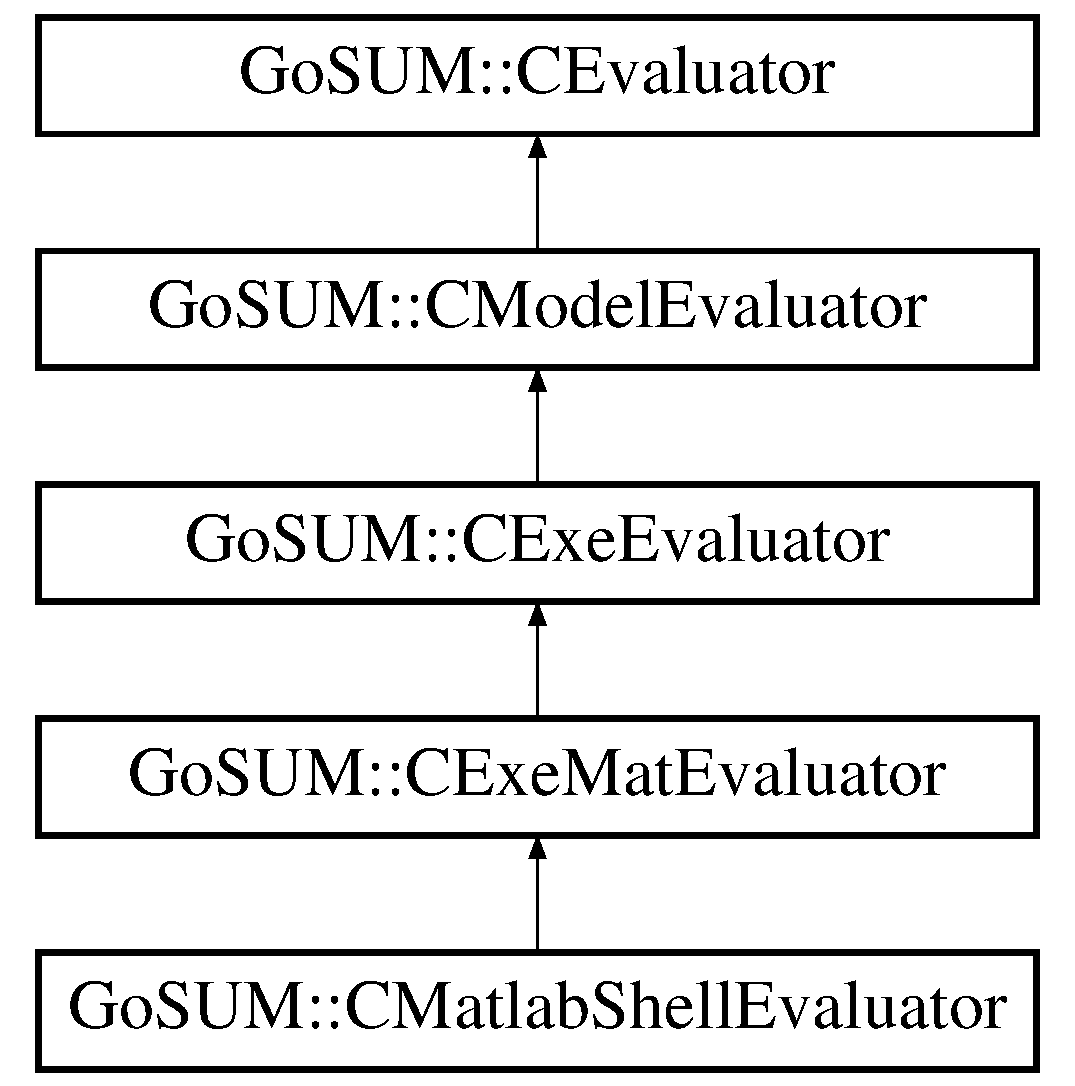
\includegraphics[height=5.000000cm]{class_go_s_u_m_1_1_c_exe_mat_evaluator}
\end{center}
\end{figure}
\subsection*{Public Member Functions}
\begin{DoxyCompactItemize}
\item 
\hyperlink{class_go_s_u_m_1_1_c_exe_mat_evaluator_a567f837642d6c8cfe6797b9af99d7a8a}{C\-Exe\-Mat\-Evaluator} ()
\item 
\hyperlink{class_go_s_u_m_1_1_c_exe_mat_evaluator_a0accdf2e03193da831c6a6f1366d42e2}{C\-Exe\-Mat\-Evaluator} (const \hyperlink{class_go_s_u_m_1_1_c_input_parameters}{C\-Input\-Parameters} $\ast$\-\_\-p\-I\-P, \hyperlink{class_go_s_u_m_1_1_c_output_states}{C\-Output\-States} $\ast$\-\_\-p\-O\-S, int \-\_\-trd\-I)
\item 
virtual \hyperlink{class_go_s_u_m_1_1_c_exe_mat_evaluator_a734c6e6f58c93948045d5ff53fef8dc1}{$\sim$\-C\-Exe\-Mat\-Evaluator} ()
\end{DoxyCompactItemize}
\subsection*{Protected Member Functions}
\begin{DoxyCompactItemize}
\item 
{\footnotesize template$<$class Archive $>$ }\\void \hyperlink{class_go_s_u_m_1_1_c_exe_mat_evaluator_a2e5121b751aaeb6f5c805cfe0312c20d}{serialize} (Archive \&ar, const unsigned int version)
\item 
virtual void \hyperlink{class_go_s_u_m_1_1_c_exe_mat_evaluator_abf90e8ece5e782c8a60cbd0021e3dfa1}{write\-To} (std\-::string \-\_\-fname, const Array\-Xd \&\-\_\-\-X, std\-::string \-\_\-\-Xname)
\item 
virtual void \hyperlink{class_go_s_u_m_1_1_c_exe_mat_evaluator_ac47387e84bc69c1e39fbe43b15465473}{read\-From} (std\-::string \-\_\-fname, Array\-Xd \&\-\_\-\-Y, std\-::string \-\_\-\-Yname)
\item 
virtual int \hyperlink{class_go_s_u_m_1_1_c_exe_mat_evaluator_a84e80ccc1d62a41f3d7881e125bee446}{read\-Size\-From} (std\-::string \-\_\-fname, std\-::string \-\_\-\-Yname)
\end{DoxyCompactItemize}
\subsection*{Protected Attributes}
\begin{DoxyCompactItemize}
\item 
\hyperlink{class_c_m_a_t_l_a_b}{C\-M\-A\-T\-L\-A\-B} \hyperlink{class_go_s_u_m_1_1_c_exe_mat_evaluator_a23d92a4142a9809c0acd60dfbb33b629}{matlab}
\end{DoxyCompactItemize}
\subsection*{Friends}
\begin{DoxyCompactItemize}
\item 
class \hyperlink{class_go_s_u_m_1_1_c_exe_mat_evaluator_ac98d07dd8f7b70e16ccb9a01abf56b9c}{boost\-::serialization\-::access}
\begin{DoxyCompactList}\small\item\em Boost serialization. \end{DoxyCompactList}\end{DoxyCompactItemize}
\subsection*{Additional Inherited Members}


\subsection{Detailed Description}
Class for the evaluator with Matlab .mat i/o and .exe. 

\subsection{Constructor \& Destructor Documentation}
\hypertarget{class_go_s_u_m_1_1_c_exe_mat_evaluator_a567f837642d6c8cfe6797b9af99d7a8a}{\index{Go\-S\-U\-M\-::\-C\-Exe\-Mat\-Evaluator@{Go\-S\-U\-M\-::\-C\-Exe\-Mat\-Evaluator}!C\-Exe\-Mat\-Evaluator@{C\-Exe\-Mat\-Evaluator}}
\index{C\-Exe\-Mat\-Evaluator@{C\-Exe\-Mat\-Evaluator}!GoSUM::CExeMatEvaluator@{Go\-S\-U\-M\-::\-C\-Exe\-Mat\-Evaluator}}
\subsubsection[{C\-Exe\-Mat\-Evaluator}]{\setlength{\rightskip}{0pt plus 5cm}Go\-S\-U\-M\-::\-C\-Exe\-Mat\-Evaluator\-::\-C\-Exe\-Mat\-Evaluator (
\begin{DoxyParamCaption}
{}
\end{DoxyParamCaption}
)\hspace{0.3cm}{\ttfamily [inline]}}}\label{class_go_s_u_m_1_1_c_exe_mat_evaluator_a567f837642d6c8cfe6797b9af99d7a8a}
\hypertarget{class_go_s_u_m_1_1_c_exe_mat_evaluator_a0accdf2e03193da831c6a6f1366d42e2}{\index{Go\-S\-U\-M\-::\-C\-Exe\-Mat\-Evaluator@{Go\-S\-U\-M\-::\-C\-Exe\-Mat\-Evaluator}!C\-Exe\-Mat\-Evaluator@{C\-Exe\-Mat\-Evaluator}}
\index{C\-Exe\-Mat\-Evaluator@{C\-Exe\-Mat\-Evaluator}!GoSUM::CExeMatEvaluator@{Go\-S\-U\-M\-::\-C\-Exe\-Mat\-Evaluator}}
\subsubsection[{C\-Exe\-Mat\-Evaluator}]{\setlength{\rightskip}{0pt plus 5cm}Go\-S\-U\-M\-::\-C\-Exe\-Mat\-Evaluator\-::\-C\-Exe\-Mat\-Evaluator (
\begin{DoxyParamCaption}
\item[{const {\bf C\-Input\-Parameters} $\ast$}]{\-\_\-p\-I\-P, }
\item[{{\bf C\-Output\-States} $\ast$}]{\-\_\-p\-O\-S, }
\item[{int}]{\-\_\-trd\-I}
\end{DoxyParamCaption}
)\hspace{0.3cm}{\ttfamily [inline]}}}\label{class_go_s_u_m_1_1_c_exe_mat_evaluator_a0accdf2e03193da831c6a6f1366d42e2}
\hypertarget{class_go_s_u_m_1_1_c_exe_mat_evaluator_a734c6e6f58c93948045d5ff53fef8dc1}{\index{Go\-S\-U\-M\-::\-C\-Exe\-Mat\-Evaluator@{Go\-S\-U\-M\-::\-C\-Exe\-Mat\-Evaluator}!$\sim$\-C\-Exe\-Mat\-Evaluator@{$\sim$\-C\-Exe\-Mat\-Evaluator}}
\index{$\sim$\-C\-Exe\-Mat\-Evaluator@{$\sim$\-C\-Exe\-Mat\-Evaluator}!GoSUM::CExeMatEvaluator@{Go\-S\-U\-M\-::\-C\-Exe\-Mat\-Evaluator}}
\subsubsection[{$\sim$\-C\-Exe\-Mat\-Evaluator}]{\setlength{\rightskip}{0pt plus 5cm}virtual Go\-S\-U\-M\-::\-C\-Exe\-Mat\-Evaluator\-::$\sim$\-C\-Exe\-Mat\-Evaluator (
\begin{DoxyParamCaption}
{}
\end{DoxyParamCaption}
)\hspace{0.3cm}{\ttfamily [inline]}, {\ttfamily [virtual]}}}\label{class_go_s_u_m_1_1_c_exe_mat_evaluator_a734c6e6f58c93948045d5ff53fef8dc1}


\subsection{Member Function Documentation}
\hypertarget{class_go_s_u_m_1_1_c_exe_mat_evaluator_ac47387e84bc69c1e39fbe43b15465473}{\index{Go\-S\-U\-M\-::\-C\-Exe\-Mat\-Evaluator@{Go\-S\-U\-M\-::\-C\-Exe\-Mat\-Evaluator}!read\-From@{read\-From}}
\index{read\-From@{read\-From}!GoSUM::CExeMatEvaluator@{Go\-S\-U\-M\-::\-C\-Exe\-Mat\-Evaluator}}
\subsubsection[{read\-From}]{\setlength{\rightskip}{0pt plus 5cm}void Go\-S\-U\-M\-::\-C\-Exe\-Mat\-Evaluator\-::read\-From (
\begin{DoxyParamCaption}
\item[{std\-::string}]{\-\_\-fname, }
\item[{Array\-Xd \&}]{\-\_\-\-Y, }
\item[{std\-::string}]{\-\_\-\-Yname}
\end{DoxyParamCaption}
)\hspace{0.3cm}{\ttfamily [protected]}, {\ttfamily [virtual]}}}\label{class_go_s_u_m_1_1_c_exe_mat_evaluator_ac47387e84bc69c1e39fbe43b15465473}


Implements \hyperlink{class_go_s_u_m_1_1_c_exe_evaluator_af453aa942a20e6494a4cd7685ace1948}{Go\-S\-U\-M\-::\-C\-Exe\-Evaluator}.

\hypertarget{class_go_s_u_m_1_1_c_exe_mat_evaluator_a84e80ccc1d62a41f3d7881e125bee446}{\index{Go\-S\-U\-M\-::\-C\-Exe\-Mat\-Evaluator@{Go\-S\-U\-M\-::\-C\-Exe\-Mat\-Evaluator}!read\-Size\-From@{read\-Size\-From}}
\index{read\-Size\-From@{read\-Size\-From}!GoSUM::CExeMatEvaluator@{Go\-S\-U\-M\-::\-C\-Exe\-Mat\-Evaluator}}
\subsubsection[{read\-Size\-From}]{\setlength{\rightskip}{0pt plus 5cm}int Go\-S\-U\-M\-::\-C\-Exe\-Mat\-Evaluator\-::read\-Size\-From (
\begin{DoxyParamCaption}
\item[{std\-::string}]{\-\_\-fname, }
\item[{std\-::string}]{\-\_\-\-Yname}
\end{DoxyParamCaption}
)\hspace{0.3cm}{\ttfamily [protected]}, {\ttfamily [virtual]}}}\label{class_go_s_u_m_1_1_c_exe_mat_evaluator_a84e80ccc1d62a41f3d7881e125bee446}


Implements \hyperlink{class_go_s_u_m_1_1_c_exe_evaluator_a1f7820ae9bd4795547dca1611769a182}{Go\-S\-U\-M\-::\-C\-Exe\-Evaluator}.

\hypertarget{class_go_s_u_m_1_1_c_exe_mat_evaluator_a2e5121b751aaeb6f5c805cfe0312c20d}{\index{Go\-S\-U\-M\-::\-C\-Exe\-Mat\-Evaluator@{Go\-S\-U\-M\-::\-C\-Exe\-Mat\-Evaluator}!serialize@{serialize}}
\index{serialize@{serialize}!GoSUM::CExeMatEvaluator@{Go\-S\-U\-M\-::\-C\-Exe\-Mat\-Evaluator}}
\subsubsection[{serialize}]{\setlength{\rightskip}{0pt plus 5cm}template$<$class Archive $>$ void Go\-S\-U\-M\-::\-C\-Exe\-Mat\-Evaluator\-::serialize (
\begin{DoxyParamCaption}
\item[{Archive \&}]{ar, }
\item[{const unsigned int}]{version}
\end{DoxyParamCaption}
)\hspace{0.3cm}{\ttfamily [protected]}}}\label{class_go_s_u_m_1_1_c_exe_mat_evaluator_a2e5121b751aaeb6f5c805cfe0312c20d}


Reimplemented from \hyperlink{class_go_s_u_m_1_1_c_exe_evaluator_adccb3c9acae9f916d8be1a9720d5bcc1}{Go\-S\-U\-M\-::\-C\-Exe\-Evaluator}.



Reimplemented in \hyperlink{class_go_s_u_m_1_1_c_matlab_shell_evaluator_af84e659441da0694bff64c2d955831b9}{Go\-S\-U\-M\-::\-C\-Matlab\-Shell\-Evaluator}.

\hypertarget{class_go_s_u_m_1_1_c_exe_mat_evaluator_abf90e8ece5e782c8a60cbd0021e3dfa1}{\index{Go\-S\-U\-M\-::\-C\-Exe\-Mat\-Evaluator@{Go\-S\-U\-M\-::\-C\-Exe\-Mat\-Evaluator}!write\-To@{write\-To}}
\index{write\-To@{write\-To}!GoSUM::CExeMatEvaluator@{Go\-S\-U\-M\-::\-C\-Exe\-Mat\-Evaluator}}
\subsubsection[{write\-To}]{\setlength{\rightskip}{0pt plus 5cm}void Go\-S\-U\-M\-::\-C\-Exe\-Mat\-Evaluator\-::write\-To (
\begin{DoxyParamCaption}
\item[{std\-::string}]{\-\_\-fname, }
\item[{const Array\-Xd \&}]{\-\_\-\-X, }
\item[{std\-::string}]{\-\_\-\-Xname}
\end{DoxyParamCaption}
)\hspace{0.3cm}{\ttfamily [protected]}, {\ttfamily [virtual]}}}\label{class_go_s_u_m_1_1_c_exe_mat_evaluator_abf90e8ece5e782c8a60cbd0021e3dfa1}


Implements \hyperlink{class_go_s_u_m_1_1_c_exe_evaluator_acb14cd0bed268c9f34a0fef4f9d8deb6}{Go\-S\-U\-M\-::\-C\-Exe\-Evaluator}.



\subsection{Friends And Related Function Documentation}
\hypertarget{class_go_s_u_m_1_1_c_exe_mat_evaluator_ac98d07dd8f7b70e16ccb9a01abf56b9c}{\index{Go\-S\-U\-M\-::\-C\-Exe\-Mat\-Evaluator@{Go\-S\-U\-M\-::\-C\-Exe\-Mat\-Evaluator}!boost\-::serialization\-::access@{boost\-::serialization\-::access}}
\index{boost\-::serialization\-::access@{boost\-::serialization\-::access}!GoSUM::CExeMatEvaluator@{Go\-S\-U\-M\-::\-C\-Exe\-Mat\-Evaluator}}
\subsubsection[{boost\-::serialization\-::access}]{\setlength{\rightskip}{0pt plus 5cm}friend class boost\-::serialization\-::access\hspace{0.3cm}{\ttfamily [friend]}}}\label{class_go_s_u_m_1_1_c_exe_mat_evaluator_ac98d07dd8f7b70e16ccb9a01abf56b9c}


Boost serialization. 



\subsection{Member Data Documentation}
\hypertarget{class_go_s_u_m_1_1_c_exe_mat_evaluator_a23d92a4142a9809c0acd60dfbb33b629}{\index{Go\-S\-U\-M\-::\-C\-Exe\-Mat\-Evaluator@{Go\-S\-U\-M\-::\-C\-Exe\-Mat\-Evaluator}!matlab@{matlab}}
\index{matlab@{matlab}!GoSUM::CExeMatEvaluator@{Go\-S\-U\-M\-::\-C\-Exe\-Mat\-Evaluator}}
\subsubsection[{matlab}]{\setlength{\rightskip}{0pt plus 5cm}{\bf C\-M\-A\-T\-L\-A\-B} Go\-S\-U\-M\-::\-C\-Exe\-Mat\-Evaluator\-::matlab\hspace{0.3cm}{\ttfamily [protected]}}}\label{class_go_s_u_m_1_1_c_exe_mat_evaluator_a23d92a4142a9809c0acd60dfbb33b629}
Object for matlab library functions. 

The documentation for this class was generated from the following files\-:\begin{DoxyCompactItemize}
\item 
C\-:/\-Development/core/\hyperlink{_original_model_8h}{Original\-Model.\-h}\item 
C\-:/\-Development/core/\hyperlink{_original_model_8cpp}{Original\-Model.\-cpp}\end{DoxyCompactItemize}

\hypertarget{class_c_exponential_c_r_v}{\section{C\-Exponential\-C\-R\-V Class Reference}
\label{class_c_exponential_c_r_v}\index{C\-Exponential\-C\-R\-V@{C\-Exponential\-C\-R\-V}}
}


Class for exponential continuous random variables derived from continuous random variables.  




{\ttfamily \#include $<$Random\-Variable.\-h$>$}

Inheritance diagram for C\-Exponential\-C\-R\-V\-:\begin{figure}[H]
\begin{center}
\leavevmode
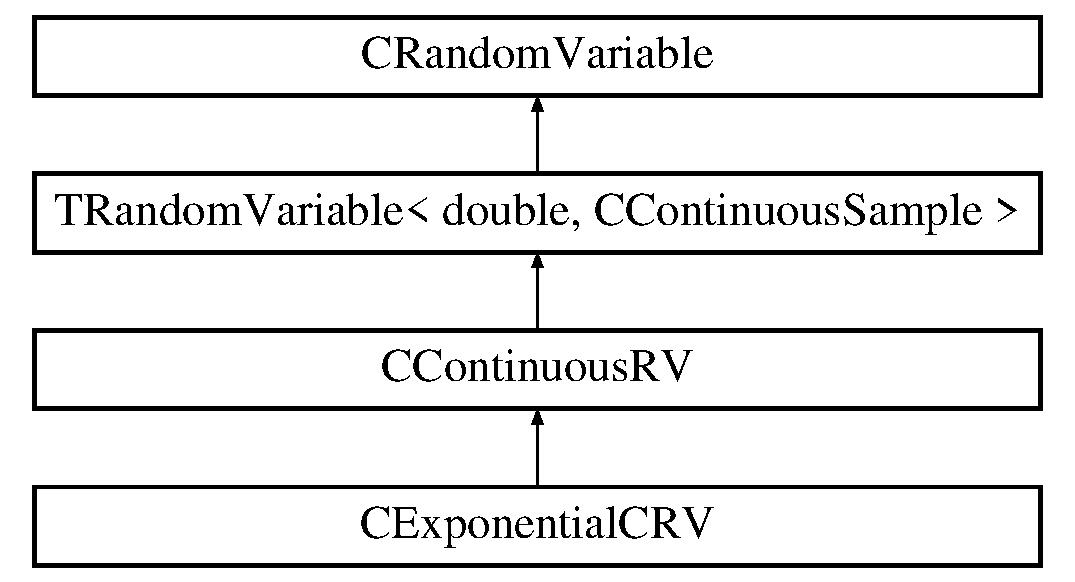
\includegraphics[height=4.000000cm]{class_c_exponential_c_r_v}
\end{center}
\end{figure}
\subsection*{Public Member Functions}
\begin{DoxyCompactItemize}
\item 
\hyperlink{class_c_exponential_c_r_v_ad31de50d93048a267d9de9dd9c765420}{C\-Exponential\-C\-R\-V} ()
\item 
virtual \hyperlink{class_c_exponential_c_r_v_ac04305397299cc8ff2ac25569af53d7e}{$\sim$\-C\-Exponential\-C\-R\-V} ()
\item 
\hyperlink{class_c_exponential_c_r_v_a33b8b0ca18ae84971af2e3aa1d0e8adf}{C\-Exponential\-C\-R\-V} (const \hyperlink{class_c_exponential_c_r_v}{C\-Exponential\-C\-R\-V} \&O)
\item 
virtual void \hyperlink{class_c_exponential_c_r_v_aeb20b2f186539ebb81dbacfae6ae5547}{set\-Distribution} (double \-\_\-lambda, double \-\_\-dp2=0)
\begin{DoxyCompactList}\small\item\em Set distribution parameters. \end{DoxyCompactList}\item 
virtual void \hyperlink{class_c_exponential_c_r_v_aae94d39cf10bce746cfa3d9541c87fc2}{set\-Distribution} (const \hyperlink{class_c_continuous_sample}{C\-Continuous\-Sample} \&\-\_\-a\-S)
\begin{DoxyCompactList}\small\item\em Set distribution parameters from sample empirical parameters. \end{DoxyCompactList}\item 
virtual double \hyperlink{class_c_exponential_c_r_v_ae4560afbed461589cfcef9bfbd9f28ee}{probability} (double \-\_\-x) const 
\begin{DoxyCompactList}\small\item\em Function that returns P\-D\-F. \end{DoxyCompactList}\item 
virtual double \hyperlink{class_c_exponential_c_r_v_acc162a5d08bb9a89bb01a0ed06558073}{cumulative} (double \-\_\-x) const 
\begin{DoxyCompactList}\small\item\em Function that returns C\-D\-F. \end{DoxyCompactList}\item 
virtual double \hyperlink{class_c_exponential_c_r_v_a6b77e823ae4b0f183edf3400fe0d799d}{min\-Value} () const 
\begin{DoxyCompactList}\small\item\em Returns minimal value of the random variable. \end{DoxyCompactList}\item 
virtual double \hyperlink{class_c_exponential_c_r_v_a61b1bfbcfcdc924c906dee4813c82b7a}{max\-Value} () const 
\begin{DoxyCompactList}\small\item\em Returns maximal value of the random variable. \end{DoxyCompactList}\item 
virtual double \hyperlink{class_c_exponential_c_r_v_a5ddbb30be4118a0795c3b56b2daee5da}{expected\-Value} () const 
\begin{DoxyCompactList}\small\item\em Returns expected value of the random variable. \end{DoxyCompactList}\item 
virtual \hyperlink{class_c_random_variable_a80d2a87c43847274138b51f7d713d7f1}{distributiontype} \hyperlink{class_c_exponential_c_r_v_adc5a1bf708580ac1ac2c35a3bb927373}{distribution\-Type} () const 
\begin{DoxyCompactList}\small\item\em Returns enum type of the random variable distribution. \end{DoxyCompactList}\item 
virtual std\-::string \hyperlink{class_c_exponential_c_r_v_a871b1ca0531fd6599d6415bfdae5bb98}{distribution\-Name} () const 
\begin{DoxyCompactList}\small\item\em Returns name of the random variable distribution. \end{DoxyCompactList}\item 
virtual Array\-Xd \hyperlink{class_c_exponential_c_r_v_ad346c5b30597b2a2a5ae3315ba8e35a4}{export\-Domain} () const 
\begin{DoxyCompactList}\small\item\em Exports domain of the random variable. \end{DoxyCompactList}\item 
double \hyperlink{class_c_exponential_c_r_v_a19c6cea6f5899279fc8a59b0c056f462}{rate\-Parameter} () const 
\begin{DoxyCompactList}\small\item\em Returns rate parameter of exponential random variable. \end{DoxyCompactList}\item 
void \hyperlink{class_c_exponential_c_r_v_a3433bb5b8060066c31c81790a252e4fe}{set\-Rate\-Parameter} (double \-\_\-lambda)
\begin{DoxyCompactList}\small\item\em Sets rate parameter of exponential random variable. \end{DoxyCompactList}\item 
virtual double \hyperlink{class_c_exponential_c_r_v_a8f0e52d384a6256289f528b1b94aaedc}{variance} () const 
\begin{DoxyCompactList}\small\item\em Returns variance of the random variable. \end{DoxyCompactList}\end{DoxyCompactItemize}
\subsection*{Protected Member Functions}
\begin{DoxyCompactItemize}
\item 
virtual double \hyperlink{class_c_exponential_c_r_v_a8e3834ea830000f7a7e76e3a7014fbad}{do\-Quantile} (double \-\_\-p) const 
\begin{DoxyCompactList}\small\item\em Quantile, formula implementation. \end{DoxyCompactList}\end{DoxyCompactItemize}
\subsection*{Private Member Functions}
\begin{DoxyCompactItemize}
\item 
{\footnotesize template$<$class Archive $>$ }\\void \hyperlink{class_c_exponential_c_r_v_abcfcc36fab68eefb9c52f64d55fc472f}{serialize} (Archive \&ar, const unsigned int version)
\end{DoxyCompactItemize}
\subsection*{Private Attributes}
\begin{DoxyCompactItemize}
\item 
double \hyperlink{class_c_exponential_c_r_v_a4bae65d53141f778e4a324f70c4658b1}{lambda}
\item 
double \hyperlink{class_c_exponential_c_r_v_a29435872622b1a114b3c5c3717239fd2}{beta}
\end{DoxyCompactItemize}
\subsection*{Friends}
\begin{DoxyCompactItemize}
\item 
class \hyperlink{class_c_exponential_c_r_v_ac98d07dd8f7b70e16ccb9a01abf56b9c}{boost\-::serialization\-::access}
\begin{DoxyCompactList}\small\item\em Boost serialization. \end{DoxyCompactList}\end{DoxyCompactItemize}
\subsection*{Additional Inherited Members}


\subsection{Detailed Description}
Class for exponential continuous random variables derived from continuous random variables. 

\subsection{Constructor \& Destructor Documentation}
\hypertarget{class_c_exponential_c_r_v_ad31de50d93048a267d9de9dd9c765420}{\index{C\-Exponential\-C\-R\-V@{C\-Exponential\-C\-R\-V}!C\-Exponential\-C\-R\-V@{C\-Exponential\-C\-R\-V}}
\index{C\-Exponential\-C\-R\-V@{C\-Exponential\-C\-R\-V}!CExponentialCRV@{C\-Exponential\-C\-R\-V}}
\subsubsection[{C\-Exponential\-C\-R\-V}]{\setlength{\rightskip}{0pt plus 5cm}C\-Exponential\-C\-R\-V\-::\-C\-Exponential\-C\-R\-V (
\begin{DoxyParamCaption}
{}
\end{DoxyParamCaption}
)\hspace{0.3cm}{\ttfamily [inline]}}}\label{class_c_exponential_c_r_v_ad31de50d93048a267d9de9dd9c765420}
\hypertarget{class_c_exponential_c_r_v_ac04305397299cc8ff2ac25569af53d7e}{\index{C\-Exponential\-C\-R\-V@{C\-Exponential\-C\-R\-V}!$\sim$\-C\-Exponential\-C\-R\-V@{$\sim$\-C\-Exponential\-C\-R\-V}}
\index{$\sim$\-C\-Exponential\-C\-R\-V@{$\sim$\-C\-Exponential\-C\-R\-V}!CExponentialCRV@{C\-Exponential\-C\-R\-V}}
\subsubsection[{$\sim$\-C\-Exponential\-C\-R\-V}]{\setlength{\rightskip}{0pt plus 5cm}virtual C\-Exponential\-C\-R\-V\-::$\sim$\-C\-Exponential\-C\-R\-V (
\begin{DoxyParamCaption}
{}
\end{DoxyParamCaption}
)\hspace{0.3cm}{\ttfamily [inline]}, {\ttfamily [virtual]}}}\label{class_c_exponential_c_r_v_ac04305397299cc8ff2ac25569af53d7e}
\hypertarget{class_c_exponential_c_r_v_a33b8b0ca18ae84971af2e3aa1d0e8adf}{\index{C\-Exponential\-C\-R\-V@{C\-Exponential\-C\-R\-V}!C\-Exponential\-C\-R\-V@{C\-Exponential\-C\-R\-V}}
\index{C\-Exponential\-C\-R\-V@{C\-Exponential\-C\-R\-V}!CExponentialCRV@{C\-Exponential\-C\-R\-V}}
\subsubsection[{C\-Exponential\-C\-R\-V}]{\setlength{\rightskip}{0pt plus 5cm}C\-Exponential\-C\-R\-V\-::\-C\-Exponential\-C\-R\-V (
\begin{DoxyParamCaption}
\item[{const {\bf C\-Exponential\-C\-R\-V} \&}]{O}
\end{DoxyParamCaption}
)\hspace{0.3cm}{\ttfamily [inline]}}}\label{class_c_exponential_c_r_v_a33b8b0ca18ae84971af2e3aa1d0e8adf}


\subsection{Member Function Documentation}
\hypertarget{class_c_exponential_c_r_v_acc162a5d08bb9a89bb01a0ed06558073}{\index{C\-Exponential\-C\-R\-V@{C\-Exponential\-C\-R\-V}!cumulative@{cumulative}}
\index{cumulative@{cumulative}!CExponentialCRV@{C\-Exponential\-C\-R\-V}}
\subsubsection[{cumulative}]{\setlength{\rightskip}{0pt plus 5cm}virtual double C\-Exponential\-C\-R\-V\-::cumulative (
\begin{DoxyParamCaption}
\item[{double}]{\-\_\-x}
\end{DoxyParamCaption}
) const\hspace{0.3cm}{\ttfamily [inline]}, {\ttfamily [virtual]}}}\label{class_c_exponential_c_r_v_acc162a5d08bb9a89bb01a0ed06558073}


Function that returns C\-D\-F. 

\hypertarget{class_c_exponential_c_r_v_a871b1ca0531fd6599d6415bfdae5bb98}{\index{C\-Exponential\-C\-R\-V@{C\-Exponential\-C\-R\-V}!distribution\-Name@{distribution\-Name}}
\index{distribution\-Name@{distribution\-Name}!CExponentialCRV@{C\-Exponential\-C\-R\-V}}
\subsubsection[{distribution\-Name}]{\setlength{\rightskip}{0pt plus 5cm}virtual std\-::string C\-Exponential\-C\-R\-V\-::distribution\-Name (
\begin{DoxyParamCaption}
{}
\end{DoxyParamCaption}
) const\hspace{0.3cm}{\ttfamily [inline]}, {\ttfamily [virtual]}}}\label{class_c_exponential_c_r_v_a871b1ca0531fd6599d6415bfdae5bb98}


Returns name of the random variable distribution. 



Implements \hyperlink{class_c_random_variable_a4b33eef7c56f9f1a83af01fa8ef2502b}{C\-Random\-Variable}.

\hypertarget{class_c_exponential_c_r_v_adc5a1bf708580ac1ac2c35a3bb927373}{\index{C\-Exponential\-C\-R\-V@{C\-Exponential\-C\-R\-V}!distribution\-Type@{distribution\-Type}}
\index{distribution\-Type@{distribution\-Type}!CExponentialCRV@{C\-Exponential\-C\-R\-V}}
\subsubsection[{distribution\-Type}]{\setlength{\rightskip}{0pt plus 5cm}virtual {\bf distributiontype} C\-Exponential\-C\-R\-V\-::distribution\-Type (
\begin{DoxyParamCaption}
{}
\end{DoxyParamCaption}
) const\hspace{0.3cm}{\ttfamily [inline]}, {\ttfamily [virtual]}}}\label{class_c_exponential_c_r_v_adc5a1bf708580ac1ac2c35a3bb927373}


Returns enum type of the random variable distribution. 



Implements \hyperlink{class_c_random_variable_a3b30589d41f4dd200bd40c8273cac2cd}{C\-Random\-Variable}.

\hypertarget{class_c_exponential_c_r_v_a8e3834ea830000f7a7e76e3a7014fbad}{\index{C\-Exponential\-C\-R\-V@{C\-Exponential\-C\-R\-V}!do\-Quantile@{do\-Quantile}}
\index{do\-Quantile@{do\-Quantile}!CExponentialCRV@{C\-Exponential\-C\-R\-V}}
\subsubsection[{do\-Quantile}]{\setlength{\rightskip}{0pt plus 5cm}virtual double C\-Exponential\-C\-R\-V\-::do\-Quantile (
\begin{DoxyParamCaption}
\item[{double}]{\-\_\-p}
\end{DoxyParamCaption}
) const\hspace{0.3cm}{\ttfamily [inline]}, {\ttfamily [protected]}, {\ttfamily [virtual]}}}\label{class_c_exponential_c_r_v_a8e3834ea830000f7a7e76e3a7014fbad}


Quantile, formula implementation. 



Implements \hyperlink{class_c_random_variable_a552ab36c8144d7154cbe3cd363eee65b}{C\-Random\-Variable}.

\hypertarget{class_c_exponential_c_r_v_a5ddbb30be4118a0795c3b56b2daee5da}{\index{C\-Exponential\-C\-R\-V@{C\-Exponential\-C\-R\-V}!expected\-Value@{expected\-Value}}
\index{expected\-Value@{expected\-Value}!CExponentialCRV@{C\-Exponential\-C\-R\-V}}
\subsubsection[{expected\-Value}]{\setlength{\rightskip}{0pt plus 5cm}virtual double C\-Exponential\-C\-R\-V\-::expected\-Value (
\begin{DoxyParamCaption}
{}
\end{DoxyParamCaption}
) const\hspace{0.3cm}{\ttfamily [inline]}, {\ttfamily [virtual]}}}\label{class_c_exponential_c_r_v_a5ddbb30be4118a0795c3b56b2daee5da}


Returns expected value of the random variable. 



Implements \hyperlink{class_c_random_variable_a6e5490d17f2b6abcf9922c8b1bd6d4ed}{C\-Random\-Variable}.

\hypertarget{class_c_exponential_c_r_v_ad346c5b30597b2a2a5ae3315ba8e35a4}{\index{C\-Exponential\-C\-R\-V@{C\-Exponential\-C\-R\-V}!export\-Domain@{export\-Domain}}
\index{export\-Domain@{export\-Domain}!CExponentialCRV@{C\-Exponential\-C\-R\-V}}
\subsubsection[{export\-Domain}]{\setlength{\rightskip}{0pt plus 5cm}Array\-Xd C\-Exponential\-C\-R\-V\-::export\-Domain (
\begin{DoxyParamCaption}
{}
\end{DoxyParamCaption}
) const\hspace{0.3cm}{\ttfamily [virtual]}}}\label{class_c_exponential_c_r_v_ad346c5b30597b2a2a5ae3315ba8e35a4}


Exports domain of the random variable. 



Implements \hyperlink{class_t_random_variable_a37fc52d5fa37493a353887242d279a27}{T\-Random\-Variable$<$ t, T $>$}.

\hypertarget{class_c_exponential_c_r_v_a61b1bfbcfcdc924c906dee4813c82b7a}{\index{C\-Exponential\-C\-R\-V@{C\-Exponential\-C\-R\-V}!max\-Value@{max\-Value}}
\index{max\-Value@{max\-Value}!CExponentialCRV@{C\-Exponential\-C\-R\-V}}
\subsubsection[{max\-Value}]{\setlength{\rightskip}{0pt plus 5cm}virtual double C\-Exponential\-C\-R\-V\-::max\-Value (
\begin{DoxyParamCaption}
{}
\end{DoxyParamCaption}
) const\hspace{0.3cm}{\ttfamily [inline]}, {\ttfamily [virtual]}}}\label{class_c_exponential_c_r_v_a61b1bfbcfcdc924c906dee4813c82b7a}


Returns maximal value of the random variable. 



Implements \hyperlink{class_c_random_variable_a48a5e98363d866f1f46568ed658479ad}{C\-Random\-Variable}.

\hypertarget{class_c_exponential_c_r_v_a6b77e823ae4b0f183edf3400fe0d799d}{\index{C\-Exponential\-C\-R\-V@{C\-Exponential\-C\-R\-V}!min\-Value@{min\-Value}}
\index{min\-Value@{min\-Value}!CExponentialCRV@{C\-Exponential\-C\-R\-V}}
\subsubsection[{min\-Value}]{\setlength{\rightskip}{0pt plus 5cm}virtual double C\-Exponential\-C\-R\-V\-::min\-Value (
\begin{DoxyParamCaption}
{}
\end{DoxyParamCaption}
) const\hspace{0.3cm}{\ttfamily [inline]}, {\ttfamily [virtual]}}}\label{class_c_exponential_c_r_v_a6b77e823ae4b0f183edf3400fe0d799d}


Returns minimal value of the random variable. 



Implements \hyperlink{class_c_random_variable_a233ddd2eedb51b09a04a8c330646f356}{C\-Random\-Variable}.

\hypertarget{class_c_exponential_c_r_v_ae4560afbed461589cfcef9bfbd9f28ee}{\index{C\-Exponential\-C\-R\-V@{C\-Exponential\-C\-R\-V}!probability@{probability}}
\index{probability@{probability}!CExponentialCRV@{C\-Exponential\-C\-R\-V}}
\subsubsection[{probability}]{\setlength{\rightskip}{0pt plus 5cm}virtual double C\-Exponential\-C\-R\-V\-::probability (
\begin{DoxyParamCaption}
\item[{double}]{\-\_\-x}
\end{DoxyParamCaption}
) const\hspace{0.3cm}{\ttfamily [inline]}, {\ttfamily [virtual]}}}\label{class_c_exponential_c_r_v_ae4560afbed461589cfcef9bfbd9f28ee}


Function that returns P\-D\-F. 

\hypertarget{class_c_exponential_c_r_v_a19c6cea6f5899279fc8a59b0c056f462}{\index{C\-Exponential\-C\-R\-V@{C\-Exponential\-C\-R\-V}!rate\-Parameter@{rate\-Parameter}}
\index{rate\-Parameter@{rate\-Parameter}!CExponentialCRV@{C\-Exponential\-C\-R\-V}}
\subsubsection[{rate\-Parameter}]{\setlength{\rightskip}{0pt plus 5cm}double C\-Exponential\-C\-R\-V\-::rate\-Parameter (
\begin{DoxyParamCaption}
{}
\end{DoxyParamCaption}
) const\hspace{0.3cm}{\ttfamily [inline]}}}\label{class_c_exponential_c_r_v_a19c6cea6f5899279fc8a59b0c056f462}


Returns rate parameter of exponential random variable. 

\hypertarget{class_c_exponential_c_r_v_abcfcc36fab68eefb9c52f64d55fc472f}{\index{C\-Exponential\-C\-R\-V@{C\-Exponential\-C\-R\-V}!serialize@{serialize}}
\index{serialize@{serialize}!CExponentialCRV@{C\-Exponential\-C\-R\-V}}
\subsubsection[{serialize}]{\setlength{\rightskip}{0pt plus 5cm}template$<$class Archive $>$ void C\-Exponential\-C\-R\-V\-::serialize (
\begin{DoxyParamCaption}
\item[{Archive \&}]{ar, }
\item[{const unsigned int}]{version}
\end{DoxyParamCaption}
)\hspace{0.3cm}{\ttfamily [private]}}}\label{class_c_exponential_c_r_v_abcfcc36fab68eefb9c52f64d55fc472f}
\hypertarget{class_c_exponential_c_r_v_aeb20b2f186539ebb81dbacfae6ae5547}{\index{C\-Exponential\-C\-R\-V@{C\-Exponential\-C\-R\-V}!set\-Distribution@{set\-Distribution}}
\index{set\-Distribution@{set\-Distribution}!CExponentialCRV@{C\-Exponential\-C\-R\-V}}
\subsubsection[{set\-Distribution}]{\setlength{\rightskip}{0pt plus 5cm}void C\-Exponential\-C\-R\-V\-::set\-Distribution (
\begin{DoxyParamCaption}
\item[{double}]{\-\_\-lambda, }
\item[{double}]{\-\_\-dp2 = {\ttfamily 0}}
\end{DoxyParamCaption}
)\hspace{0.3cm}{\ttfamily [virtual]}}}\label{class_c_exponential_c_r_v_aeb20b2f186539ebb81dbacfae6ae5547}


Set distribution parameters. 

\hypertarget{class_c_exponential_c_r_v_aae94d39cf10bce746cfa3d9541c87fc2}{\index{C\-Exponential\-C\-R\-V@{C\-Exponential\-C\-R\-V}!set\-Distribution@{set\-Distribution}}
\index{set\-Distribution@{set\-Distribution}!CExponentialCRV@{C\-Exponential\-C\-R\-V}}
\subsubsection[{set\-Distribution}]{\setlength{\rightskip}{0pt plus 5cm}virtual void C\-Exponential\-C\-R\-V\-::set\-Distribution (
\begin{DoxyParamCaption}
\item[{const {\bf C\-Continuous\-Sample} \&}]{\-\_\-a\-S}
\end{DoxyParamCaption}
)\hspace{0.3cm}{\ttfamily [inline]}, {\ttfamily [virtual]}}}\label{class_c_exponential_c_r_v_aae94d39cf10bce746cfa3d9541c87fc2}


Set distribution parameters from sample empirical parameters. 

\hypertarget{class_c_exponential_c_r_v_a3433bb5b8060066c31c81790a252e4fe}{\index{C\-Exponential\-C\-R\-V@{C\-Exponential\-C\-R\-V}!set\-Rate\-Parameter@{set\-Rate\-Parameter}}
\index{set\-Rate\-Parameter@{set\-Rate\-Parameter}!CExponentialCRV@{C\-Exponential\-C\-R\-V}}
\subsubsection[{set\-Rate\-Parameter}]{\setlength{\rightskip}{0pt plus 5cm}void C\-Exponential\-C\-R\-V\-::set\-Rate\-Parameter (
\begin{DoxyParamCaption}
\item[{double}]{\-\_\-lambda}
\end{DoxyParamCaption}
)\hspace{0.3cm}{\ttfamily [inline]}}}\label{class_c_exponential_c_r_v_a3433bb5b8060066c31c81790a252e4fe}


Sets rate parameter of exponential random variable. 

\hypertarget{class_c_exponential_c_r_v_a8f0e52d384a6256289f528b1b94aaedc}{\index{C\-Exponential\-C\-R\-V@{C\-Exponential\-C\-R\-V}!variance@{variance}}
\index{variance@{variance}!CExponentialCRV@{C\-Exponential\-C\-R\-V}}
\subsubsection[{variance}]{\setlength{\rightskip}{0pt plus 5cm}virtual double C\-Exponential\-C\-R\-V\-::variance (
\begin{DoxyParamCaption}
{}
\end{DoxyParamCaption}
) const\hspace{0.3cm}{\ttfamily [inline]}, {\ttfamily [virtual]}}}\label{class_c_exponential_c_r_v_a8f0e52d384a6256289f528b1b94aaedc}


Returns variance of the random variable. 



Implements \hyperlink{class_c_random_variable_a3b0b87c4aab74c0406cd8321b8b96747}{C\-Random\-Variable}.



\subsection{Friends And Related Function Documentation}
\hypertarget{class_c_exponential_c_r_v_ac98d07dd8f7b70e16ccb9a01abf56b9c}{\index{C\-Exponential\-C\-R\-V@{C\-Exponential\-C\-R\-V}!boost\-::serialization\-::access@{boost\-::serialization\-::access}}
\index{boost\-::serialization\-::access@{boost\-::serialization\-::access}!CExponentialCRV@{C\-Exponential\-C\-R\-V}}
\subsubsection[{boost\-::serialization\-::access}]{\setlength{\rightskip}{0pt plus 5cm}friend class boost\-::serialization\-::access\hspace{0.3cm}{\ttfamily [friend]}}}\label{class_c_exponential_c_r_v_ac98d07dd8f7b70e16ccb9a01abf56b9c}


Boost serialization. 



\subsection{Member Data Documentation}
\hypertarget{class_c_exponential_c_r_v_a29435872622b1a114b3c5c3717239fd2}{\index{C\-Exponential\-C\-R\-V@{C\-Exponential\-C\-R\-V}!beta@{beta}}
\index{beta@{beta}!CExponentialCRV@{C\-Exponential\-C\-R\-V}}
\subsubsection[{beta}]{\setlength{\rightskip}{0pt plus 5cm}double C\-Exponential\-C\-R\-V\-::beta\hspace{0.3cm}{\ttfamily [private]}}}\label{class_c_exponential_c_r_v_a29435872622b1a114b3c5c3717239fd2}
Distribution parameters\-: rate parameter beta=1/lambda. \hypertarget{class_c_exponential_c_r_v_a4bae65d53141f778e4a324f70c4658b1}{\index{C\-Exponential\-C\-R\-V@{C\-Exponential\-C\-R\-V}!lambda@{lambda}}
\index{lambda@{lambda}!CExponentialCRV@{C\-Exponential\-C\-R\-V}}
\subsubsection[{lambda}]{\setlength{\rightskip}{0pt plus 5cm}double C\-Exponential\-C\-R\-V\-::lambda\hspace{0.3cm}{\ttfamily [private]}}}\label{class_c_exponential_c_r_v_a4bae65d53141f778e4a324f70c4658b1}


The documentation for this class was generated from the following files\-:\begin{DoxyCompactItemize}
\item 
C\-:/\-Development/core/\hyperlink{_random_variable_8h}{Random\-Variable.\-h}\item 
C\-:/\-Development/core/\hyperlink{_random_variable_8cpp}{Random\-Variable.\-cpp}\end{DoxyCompactItemize}

\hypertarget{class_c_f_f_t_w}{\section{C\-F\-F\-T\-W Class Reference}
\label{class_c_f_f_t_w}\index{C\-F\-F\-T\-W@{C\-F\-F\-T\-W}}
}


Class interface for F\-F\-T\-W's libfftw library.  




{\ttfamily \#include $<$F\-F\-T\-W\-Library.\-h$>$}

\subsection*{Public Member Functions}
\begin{DoxyCompactItemize}
\item 
\hyperlink{class_c_f_f_t_w_a8306e328b4e54257f5c38b367dc93ff8}{C\-F\-F\-T\-W} ()
\item 
virtual \hyperlink{class_c_f_f_t_w_a29f9a0d485628e06e8db134dd48a81a7}{$\sim$\-C\-F\-F\-T\-W} ()
\item 
Array\-Xd \hyperlink{class_c_f_f_t_w_a83218155fb070ed39b07cc8bd956f188}{discrete\-Cosine\-Transform} (const Array\-Xd \&in)
\begin{DoxyCompactList}\small\item\em Computes discrete cosine transform using fftw. \end{DoxyCompactList}\item 
Array\-Xd \hyperlink{class_c_f_f_t_w_aa40c9ada6c75d44cbd49d98e094b412b}{inverse\-Discrete\-Cosine\-Transform} (const Array\-Xd \&in)
\begin{DoxyCompactList}\small\item\em Computes inverse discrete cosine transform using fftw. \end{DoxyCompactList}\end{DoxyCompactItemize}


\subsection{Detailed Description}
Class interface for F\-F\-T\-W's libfftw library. 

\subsection{Constructor \& Destructor Documentation}
\hypertarget{class_c_f_f_t_w_a8306e328b4e54257f5c38b367dc93ff8}{\index{C\-F\-F\-T\-W@{C\-F\-F\-T\-W}!C\-F\-F\-T\-W@{C\-F\-F\-T\-W}}
\index{C\-F\-F\-T\-W@{C\-F\-F\-T\-W}!CFFTW@{C\-F\-F\-T\-W}}
\subsubsection[{C\-F\-F\-T\-W}]{\setlength{\rightskip}{0pt plus 5cm}C\-F\-F\-T\-W\-::\-C\-F\-F\-T\-W (
\begin{DoxyParamCaption}
{}
\end{DoxyParamCaption}
)\hspace{0.3cm}{\ttfamily [inline]}}}\label{class_c_f_f_t_w_a8306e328b4e54257f5c38b367dc93ff8}
\hypertarget{class_c_f_f_t_w_a29f9a0d485628e06e8db134dd48a81a7}{\index{C\-F\-F\-T\-W@{C\-F\-F\-T\-W}!$\sim$\-C\-F\-F\-T\-W@{$\sim$\-C\-F\-F\-T\-W}}
\index{$\sim$\-C\-F\-F\-T\-W@{$\sim$\-C\-F\-F\-T\-W}!CFFTW@{C\-F\-F\-T\-W}}
\subsubsection[{$\sim$\-C\-F\-F\-T\-W}]{\setlength{\rightskip}{0pt plus 5cm}virtual C\-F\-F\-T\-W\-::$\sim$\-C\-F\-F\-T\-W (
\begin{DoxyParamCaption}
{}
\end{DoxyParamCaption}
)\hspace{0.3cm}{\ttfamily [inline]}, {\ttfamily [virtual]}}}\label{class_c_f_f_t_w_a29f9a0d485628e06e8db134dd48a81a7}


\subsection{Member Function Documentation}
\hypertarget{class_c_f_f_t_w_a83218155fb070ed39b07cc8bd956f188}{\index{C\-F\-F\-T\-W@{C\-F\-F\-T\-W}!discrete\-Cosine\-Transform@{discrete\-Cosine\-Transform}}
\index{discrete\-Cosine\-Transform@{discrete\-Cosine\-Transform}!CFFTW@{C\-F\-F\-T\-W}}
\subsubsection[{discrete\-Cosine\-Transform}]{\setlength{\rightskip}{0pt plus 5cm}Array\-Xd C\-F\-F\-T\-W\-::discrete\-Cosine\-Transform (
\begin{DoxyParamCaption}
\item[{const Array\-Xd \&}]{in}
\end{DoxyParamCaption}
)}}\label{class_c_f_f_t_w_a83218155fb070ed39b07cc8bd956f188}


Computes discrete cosine transform using fftw. 

\hypertarget{class_c_f_f_t_w_aa40c9ada6c75d44cbd49d98e094b412b}{\index{C\-F\-F\-T\-W@{C\-F\-F\-T\-W}!inverse\-Discrete\-Cosine\-Transform@{inverse\-Discrete\-Cosine\-Transform}}
\index{inverse\-Discrete\-Cosine\-Transform@{inverse\-Discrete\-Cosine\-Transform}!CFFTW@{C\-F\-F\-T\-W}}
\subsubsection[{inverse\-Discrete\-Cosine\-Transform}]{\setlength{\rightskip}{0pt plus 5cm}Array\-Xd C\-F\-F\-T\-W\-::inverse\-Discrete\-Cosine\-Transform (
\begin{DoxyParamCaption}
\item[{const Array\-Xd \&}]{in}
\end{DoxyParamCaption}
)}}\label{class_c_f_f_t_w_aa40c9ada6c75d44cbd49d98e094b412b}


Computes inverse discrete cosine transform using fftw. 



The documentation for this class was generated from the following files\-:\begin{DoxyCompactItemize}
\item 
C\-:/\-Development/core/\hyperlink{_f_f_t_w_library_8h}{F\-F\-T\-W\-Library.\-h}\item 
C\-:/\-Development/core/\hyperlink{_f_f_t_w_library_8cpp}{F\-F\-T\-W\-Library.\-cpp}\end{DoxyCompactItemize}

\hypertarget{class_c_g_a_model_optimization}{\section{C\-G\-A\-Model\-Optimization Class Reference}
\label{class_c_g_a_model_optimization}\index{C\-G\-A\-Model\-Optimization@{C\-G\-A\-Model\-Optimization}}
}


Class for the genetic algorithm, i.\-e. interface for G\-A\-L\-I\-B.  




{\ttfamily \#include $<$G\-A\-Optimization.\-h$>$}

\subsection*{Public Member Functions}
\begin{DoxyCompactItemize}
\item 
\hyperlink{class_c_g_a_model_optimization_a3e7d2d1af84f747b69521af1b3cb98b1}{C\-G\-A\-Model\-Optimization} ()
\item 
virtual \hyperlink{class_c_g_a_model_optimization_a932712b68c1d4ee55338d8ba034bddca}{$\sim$\-C\-G\-A\-Model\-Optimization} ()
\item 
Array\-Xd \hyperlink{class_c_g_a_model_optimization_a9bb25fd06282c76aae2faa19b16786a7}{optimize} (\hyperlink{class_c_optimization_problem}{C\-Optimization\-Problem} $\ast$\-\_\-p\-S\-O\-P, std\-::ostream \&\-\_\-out=std\-::cout)
\begin{DoxyCompactList}\small\item\em Solves the optimizations problem. \end{DoxyCompactList}\item 
int \hyperlink{class_c_g_a_model_optimization_a8dd868da2dc8b1a1e648e1e1ec34d02f}{progress\-Steps\-Size} () const 
\begin{DoxyCompactList}\small\item\em Returns progress steps size. \end{DoxyCompactList}\item 
int \hyperlink{class_c_g_a_model_optimization_a6afd417c7d16c6e721aa3aa6b84f5b60}{population\-Size} () const 
\begin{DoxyCompactList}\small\item\em Returns population size. \end{DoxyCompactList}\item 
void \hyperlink{class_c_g_a_model_optimization_abb540bb6a17610b32bfea0863a3b4eb6}{set\-Population\-Size} (int \-\_\-popsize)
\begin{DoxyCompactList}\small\item\em Sets population size. \end{DoxyCompactList}\end{DoxyCompactItemize}
\subsection*{Static Public Member Functions}
\begin{DoxyCompactItemize}
\item 
static Array\-Xd \hyperlink{class_c_g_a_model_optimization_a43c6ca120a99ced7c095dfc3c4422381}{G\-A\-Genome2\-Array\-Xd} (const G\-A\-Genome \&g)
\begin{DoxyCompactList}\small\item\em Converts G\-A\-Genome -\/$>$ hpyercube point. \end{DoxyCompactList}\item 
static float \hyperlink{class_c_g_a_model_optimization_a3da8eb17ef08ba4b3e87b8f7d902878e}{Fitness} (G\-A\-Genome \&g)
\begin{DoxyCompactList}\small\item\em Evalutes fitness of an individual. \end{DoxyCompactList}\end{DoxyCompactItemize}
\subsection*{Protected Member Functions}
\begin{DoxyCompactItemize}
\item 
{\footnotesize template$<$class Archive $>$ }\\void \hyperlink{class_c_g_a_model_optimization_ad2294cc27928439a39c86cc0899c4a15}{serialize} (Archive \&ar, const unsigned int version)
\end{DoxyCompactItemize}
\subsection*{Protected Attributes}
\begin{DoxyCompactItemize}
\item 
int \hyperlink{class_c_g_a_model_optimization_a630bb8f0d92f88da6923cabbe2dc6bbd}{popsize}
\item 
Array\-Xd \hyperlink{class_c_g_a_model_optimization_a20e94024ae32a632442dfb9de308c81e}{Xbest}
\item 
double \hyperlink{class_c_g_a_model_optimization_aa29eb539bc5208c83e5507942e45de91}{ybest}
\end{DoxyCompactItemize}
\subsection*{Static Protected Attributes}
\begin{DoxyCompactItemize}
\item 
static \hyperlink{class_c_optimization_problem}{C\-Optimization\-Problem} $\ast$ \hyperlink{class_c_g_a_model_optimization_a6b925befb13a952f6f8bae588cce6106}{p\-O\-P} = N\-U\-L\-L
\begin{DoxyCompactList}\small\item\em Points to the optimization problem. \end{DoxyCompactList}\item 
static double \hyperlink{class_c_g_a_model_optimization_ab1915d63ecd7b920e93e3171724f3e71}{C} = 1.e+2
\begin{DoxyCompactList}\small\item\em Constant added to get positive fitness. \end{DoxyCompactList}\end{DoxyCompactItemize}
\subsection*{Friends}
\begin{DoxyCompactItemize}
\item 
class \hyperlink{class_c_g_a_model_optimization_ac98d07dd8f7b70e16ccb9a01abf56b9c}{boost\-::serialization\-::access}
\begin{DoxyCompactList}\small\item\em Boost serialization. \end{DoxyCompactList}\end{DoxyCompactItemize}


\subsection{Detailed Description}
Class for the genetic algorithm, i.\-e. interface for G\-A\-L\-I\-B. 

\subsection{Constructor \& Destructor Documentation}
\hypertarget{class_c_g_a_model_optimization_a3e7d2d1af84f747b69521af1b3cb98b1}{\index{C\-G\-A\-Model\-Optimization@{C\-G\-A\-Model\-Optimization}!C\-G\-A\-Model\-Optimization@{C\-G\-A\-Model\-Optimization}}
\index{C\-G\-A\-Model\-Optimization@{C\-G\-A\-Model\-Optimization}!CGAModelOptimization@{C\-G\-A\-Model\-Optimization}}
\subsubsection[{C\-G\-A\-Model\-Optimization}]{\setlength{\rightskip}{0pt plus 5cm}C\-G\-A\-Model\-Optimization\-::\-C\-G\-A\-Model\-Optimization (
\begin{DoxyParamCaption}
{}
\end{DoxyParamCaption}
)\hspace{0.3cm}{\ttfamily [inline]}}}\label{class_c_g_a_model_optimization_a3e7d2d1af84f747b69521af1b3cb98b1}
\hypertarget{class_c_g_a_model_optimization_a932712b68c1d4ee55338d8ba034bddca}{\index{C\-G\-A\-Model\-Optimization@{C\-G\-A\-Model\-Optimization}!$\sim$\-C\-G\-A\-Model\-Optimization@{$\sim$\-C\-G\-A\-Model\-Optimization}}
\index{$\sim$\-C\-G\-A\-Model\-Optimization@{$\sim$\-C\-G\-A\-Model\-Optimization}!CGAModelOptimization@{C\-G\-A\-Model\-Optimization}}
\subsubsection[{$\sim$\-C\-G\-A\-Model\-Optimization}]{\setlength{\rightskip}{0pt plus 5cm}virtual C\-G\-A\-Model\-Optimization\-::$\sim$\-C\-G\-A\-Model\-Optimization (
\begin{DoxyParamCaption}
{}
\end{DoxyParamCaption}
)\hspace{0.3cm}{\ttfamily [inline]}, {\ttfamily [virtual]}}}\label{class_c_g_a_model_optimization_a932712b68c1d4ee55338d8ba034bddca}


\subsection{Member Function Documentation}
\hypertarget{class_c_g_a_model_optimization_a3da8eb17ef08ba4b3e87b8f7d902878e}{\index{C\-G\-A\-Model\-Optimization@{C\-G\-A\-Model\-Optimization}!Fitness@{Fitness}}
\index{Fitness@{Fitness}!CGAModelOptimization@{C\-G\-A\-Model\-Optimization}}
\subsubsection[{Fitness}]{\setlength{\rightskip}{0pt plus 5cm}float C\-G\-A\-Model\-Optimization\-::\-Fitness (
\begin{DoxyParamCaption}
\item[{G\-A\-Genome \&}]{g}
\end{DoxyParamCaption}
)\hspace{0.3cm}{\ttfamily [static]}}}\label{class_c_g_a_model_optimization_a3da8eb17ef08ba4b3e87b8f7d902878e}


Evalutes fitness of an individual. 

\hypertarget{class_c_g_a_model_optimization_a43c6ca120a99ced7c095dfc3c4422381}{\index{C\-G\-A\-Model\-Optimization@{C\-G\-A\-Model\-Optimization}!G\-A\-Genome2\-Array\-Xd@{G\-A\-Genome2\-Array\-Xd}}
\index{G\-A\-Genome2\-Array\-Xd@{G\-A\-Genome2\-Array\-Xd}!CGAModelOptimization@{C\-G\-A\-Model\-Optimization}}
\subsubsection[{G\-A\-Genome2\-Array\-Xd}]{\setlength{\rightskip}{0pt plus 5cm}Array\-Xd C\-G\-A\-Model\-Optimization\-::\-G\-A\-Genome2\-Array\-Xd (
\begin{DoxyParamCaption}
\item[{const G\-A\-Genome \&}]{g}
\end{DoxyParamCaption}
)\hspace{0.3cm}{\ttfamily [static]}}}\label{class_c_g_a_model_optimization_a43c6ca120a99ced7c095dfc3c4422381}


Converts G\-A\-Genome -\/$>$ hpyercube point. 

\hypertarget{class_c_g_a_model_optimization_a9bb25fd06282c76aae2faa19b16786a7}{\index{C\-G\-A\-Model\-Optimization@{C\-G\-A\-Model\-Optimization}!optimize@{optimize}}
\index{optimize@{optimize}!CGAModelOptimization@{C\-G\-A\-Model\-Optimization}}
\subsubsection[{optimize}]{\setlength{\rightskip}{0pt plus 5cm}Array\-Xd C\-G\-A\-Model\-Optimization\-::optimize (
\begin{DoxyParamCaption}
\item[{{\bf C\-Optimization\-Problem} $\ast$}]{\-\_\-p\-S\-O\-P, }
\item[{std\-::ostream \&}]{\-\_\-out = {\ttfamily std\-:\-:cout}}
\end{DoxyParamCaption}
)}}\label{class_c_g_a_model_optimization_a9bb25fd06282c76aae2faa19b16786a7}


Solves the optimizations problem. 

\hypertarget{class_c_g_a_model_optimization_a6afd417c7d16c6e721aa3aa6b84f5b60}{\index{C\-G\-A\-Model\-Optimization@{C\-G\-A\-Model\-Optimization}!population\-Size@{population\-Size}}
\index{population\-Size@{population\-Size}!CGAModelOptimization@{C\-G\-A\-Model\-Optimization}}
\subsubsection[{population\-Size}]{\setlength{\rightskip}{0pt plus 5cm}int C\-G\-A\-Model\-Optimization\-::population\-Size (
\begin{DoxyParamCaption}
{}
\end{DoxyParamCaption}
) const\hspace{0.3cm}{\ttfamily [inline]}}}\label{class_c_g_a_model_optimization_a6afd417c7d16c6e721aa3aa6b84f5b60}


Returns population size. 

\hypertarget{class_c_g_a_model_optimization_a8dd868da2dc8b1a1e648e1e1ec34d02f}{\index{C\-G\-A\-Model\-Optimization@{C\-G\-A\-Model\-Optimization}!progress\-Steps\-Size@{progress\-Steps\-Size}}
\index{progress\-Steps\-Size@{progress\-Steps\-Size}!CGAModelOptimization@{C\-G\-A\-Model\-Optimization}}
\subsubsection[{progress\-Steps\-Size}]{\setlength{\rightskip}{0pt plus 5cm}int C\-G\-A\-Model\-Optimization\-::progress\-Steps\-Size (
\begin{DoxyParamCaption}
{}
\end{DoxyParamCaption}
) const\hspace{0.3cm}{\ttfamily [inline]}}}\label{class_c_g_a_model_optimization_a8dd868da2dc8b1a1e648e1e1ec34d02f}


Returns progress steps size. 

\hypertarget{class_c_g_a_model_optimization_ad2294cc27928439a39c86cc0899c4a15}{\index{C\-G\-A\-Model\-Optimization@{C\-G\-A\-Model\-Optimization}!serialize@{serialize}}
\index{serialize@{serialize}!CGAModelOptimization@{C\-G\-A\-Model\-Optimization}}
\subsubsection[{serialize}]{\setlength{\rightskip}{0pt plus 5cm}template$<$class Archive $>$ void C\-G\-A\-Model\-Optimization\-::serialize (
\begin{DoxyParamCaption}
\item[{Archive \&}]{ar, }
\item[{const unsigned int}]{version}
\end{DoxyParamCaption}
)\hspace{0.3cm}{\ttfamily [protected]}}}\label{class_c_g_a_model_optimization_ad2294cc27928439a39c86cc0899c4a15}
\hypertarget{class_c_g_a_model_optimization_abb540bb6a17610b32bfea0863a3b4eb6}{\index{C\-G\-A\-Model\-Optimization@{C\-G\-A\-Model\-Optimization}!set\-Population\-Size@{set\-Population\-Size}}
\index{set\-Population\-Size@{set\-Population\-Size}!CGAModelOptimization@{C\-G\-A\-Model\-Optimization}}
\subsubsection[{set\-Population\-Size}]{\setlength{\rightskip}{0pt plus 5cm}void C\-G\-A\-Model\-Optimization\-::set\-Population\-Size (
\begin{DoxyParamCaption}
\item[{int}]{\-\_\-popsize}
\end{DoxyParamCaption}
)\hspace{0.3cm}{\ttfamily [inline]}}}\label{class_c_g_a_model_optimization_abb540bb6a17610b32bfea0863a3b4eb6}


Sets population size. 



\subsection{Friends And Related Function Documentation}
\hypertarget{class_c_g_a_model_optimization_ac98d07dd8f7b70e16ccb9a01abf56b9c}{\index{C\-G\-A\-Model\-Optimization@{C\-G\-A\-Model\-Optimization}!boost\-::serialization\-::access@{boost\-::serialization\-::access}}
\index{boost\-::serialization\-::access@{boost\-::serialization\-::access}!CGAModelOptimization@{C\-G\-A\-Model\-Optimization}}
\subsubsection[{boost\-::serialization\-::access}]{\setlength{\rightskip}{0pt plus 5cm}friend class boost\-::serialization\-::access\hspace{0.3cm}{\ttfamily [friend]}}}\label{class_c_g_a_model_optimization_ac98d07dd8f7b70e16ccb9a01abf56b9c}


Boost serialization. 



\subsection{Member Data Documentation}
\hypertarget{class_c_g_a_model_optimization_ab1915d63ecd7b920e93e3171724f3e71}{\index{C\-G\-A\-Model\-Optimization@{C\-G\-A\-Model\-Optimization}!C@{C}}
\index{C@{C}!CGAModelOptimization@{C\-G\-A\-Model\-Optimization}}
\subsubsection[{C}]{\setlength{\rightskip}{0pt plus 5cm}double C\-G\-A\-Model\-Optimization\-::\-C = 1.e+2\hspace{0.3cm}{\ttfamily [static]}, {\ttfamily [protected]}}}\label{class_c_g_a_model_optimization_ab1915d63ecd7b920e93e3171724f3e71}


Constant added to get positive fitness. 

\hypertarget{class_c_g_a_model_optimization_a6b925befb13a952f6f8bae588cce6106}{\index{C\-G\-A\-Model\-Optimization@{C\-G\-A\-Model\-Optimization}!p\-O\-P@{p\-O\-P}}
\index{p\-O\-P@{p\-O\-P}!CGAModelOptimization@{C\-G\-A\-Model\-Optimization}}
\subsubsection[{p\-O\-P}]{\setlength{\rightskip}{0pt plus 5cm}{\bf C\-Optimization\-Problem} $\ast$ C\-G\-A\-Model\-Optimization\-::p\-O\-P = N\-U\-L\-L\hspace{0.3cm}{\ttfamily [static]}, {\ttfamily [protected]}}}\label{class_c_g_a_model_optimization_a6b925befb13a952f6f8bae588cce6106}


Points to the optimization problem. 

\hypertarget{class_c_g_a_model_optimization_a630bb8f0d92f88da6923cabbe2dc6bbd}{\index{C\-G\-A\-Model\-Optimization@{C\-G\-A\-Model\-Optimization}!popsize@{popsize}}
\index{popsize@{popsize}!CGAModelOptimization@{C\-G\-A\-Model\-Optimization}}
\subsubsection[{popsize}]{\setlength{\rightskip}{0pt plus 5cm}int C\-G\-A\-Model\-Optimization\-::popsize\hspace{0.3cm}{\ttfamily [protected]}}}\label{class_c_g_a_model_optimization_a630bb8f0d92f88da6923cabbe2dc6bbd}
\hypertarget{class_c_g_a_model_optimization_a20e94024ae32a632442dfb9de308c81e}{\index{C\-G\-A\-Model\-Optimization@{C\-G\-A\-Model\-Optimization}!Xbest@{Xbest}}
\index{Xbest@{Xbest}!CGAModelOptimization@{C\-G\-A\-Model\-Optimization}}
\subsubsection[{Xbest}]{\setlength{\rightskip}{0pt plus 5cm}Array\-Xd C\-G\-A\-Model\-Optimization\-::\-Xbest\hspace{0.3cm}{\ttfamily [protected]}}}\label{class_c_g_a_model_optimization_a20e94024ae32a632442dfb9de308c81e}
\hypertarget{class_c_g_a_model_optimization_aa29eb539bc5208c83e5507942e45de91}{\index{C\-G\-A\-Model\-Optimization@{C\-G\-A\-Model\-Optimization}!ybest@{ybest}}
\index{ybest@{ybest}!CGAModelOptimization@{C\-G\-A\-Model\-Optimization}}
\subsubsection[{ybest}]{\setlength{\rightskip}{0pt plus 5cm}double C\-G\-A\-Model\-Optimization\-::ybest\hspace{0.3cm}{\ttfamily [protected]}}}\label{class_c_g_a_model_optimization_aa29eb539bc5208c83e5507942e45de91}


The documentation for this class was generated from the following files\-:\begin{DoxyCompactItemize}
\item 
C\-:/\-Development/core/\hyperlink{_g_a_optimization_8h}{G\-A\-Optimization.\-h}\item 
C\-:/\-Development/core/\hyperlink{_g_a_optimization_8cpp}{G\-A\-Optimization.\-cpp}\end{DoxyCompactItemize}

\hypertarget{class_c_gaussian_c_r_v}{\section{C\-Gaussian\-C\-R\-V Class Reference}
\label{class_c_gaussian_c_r_v}\index{C\-Gaussian\-C\-R\-V@{C\-Gaussian\-C\-R\-V}}
}


Class for Gaussian continuous random variables derived from continuous random variables.  




{\ttfamily \#include $<$Random\-Variable.\-h$>$}

Inheritance diagram for C\-Gaussian\-C\-R\-V\-:\begin{figure}[H]
\begin{center}
\leavevmode
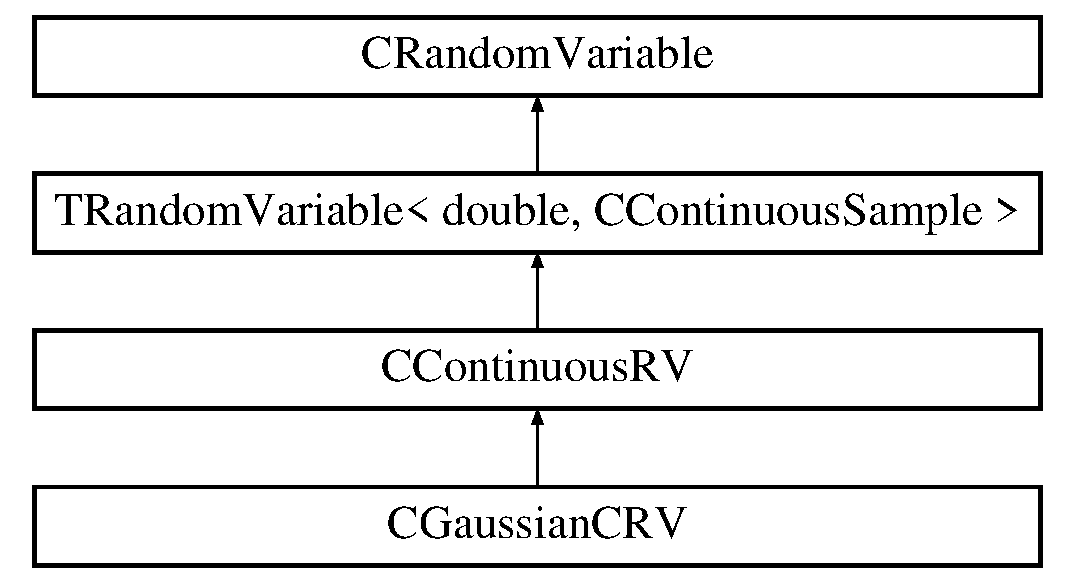
\includegraphics[height=4.000000cm]{class_c_gaussian_c_r_v}
\end{center}
\end{figure}
\subsection*{Public Member Functions}
\begin{DoxyCompactItemize}
\item 
\hyperlink{class_c_gaussian_c_r_v_ad0467f60ab0086154121f023a37c4db2}{C\-Gaussian\-C\-R\-V} ()
\item 
virtual \hyperlink{class_c_gaussian_c_r_v_ad5bd8a3b2e6c4a811315652f0d98e9c7}{$\sim$\-C\-Gaussian\-C\-R\-V} ()
\item 
\hyperlink{class_c_gaussian_c_r_v_a888a11c81805e8fecad9887e4f75bca7}{C\-Gaussian\-C\-R\-V} (const \hyperlink{class_c_gaussian_c_r_v}{C\-Gaussian\-C\-R\-V} \&O)
\item 
virtual void \hyperlink{class_c_gaussian_c_r_v_a450fc3a79bfc1646ae43bf1ba6d23133}{set\-Distribution} (double \-\_\-mu, double \-\_\-sigma)
\begin{DoxyCompactList}\small\item\em Set distribution parameters. \end{DoxyCompactList}\item 
virtual void \hyperlink{class_c_gaussian_c_r_v_a48de04775bfdf8d0e2c5a2aa73eb500e}{set\-Distribution} (const \hyperlink{class_c_continuous_sample}{C\-Continuous\-Sample} \&\-\_\-a\-S)
\begin{DoxyCompactList}\small\item\em Set distribution parameters from sample empirical parameters. \end{DoxyCompactList}\item 
virtual double \hyperlink{class_c_gaussian_c_r_v_a14ac3654b0527aa3354d60d120abd1cb}{probability} (double \-\_\-x) const 
\begin{DoxyCompactList}\small\item\em Function that returns P\-D\-F. \end{DoxyCompactList}\item 
virtual double \hyperlink{class_c_gaussian_c_r_v_a226e37ee1c3a14d9f0dbf691267e27a1}{cumulative} (double \-\_\-x) const 
\begin{DoxyCompactList}\small\item\em Function that returns C\-D\-F. \end{DoxyCompactList}\item 
virtual double \hyperlink{class_c_gaussian_c_r_v_a89ab0f2b91ef9bb45f29bdf8f851003e}{min\-Value} () const 
\begin{DoxyCompactList}\small\item\em Returns minimal value of the random variable. \end{DoxyCompactList}\item 
virtual double \hyperlink{class_c_gaussian_c_r_v_a0b51f23a85bd3ab3e78556e7db197c49}{max\-Value} () const 
\begin{DoxyCompactList}\small\item\em Returns maximal value of the random variable. \end{DoxyCompactList}\item 
virtual double \hyperlink{class_c_gaussian_c_r_v_a20650fed2a45e12bfc72a98efb6c8e31}{expected\-Value} () const 
\begin{DoxyCompactList}\small\item\em Returns expected value of the random variable. \end{DoxyCompactList}\item 
virtual \hyperlink{class_c_random_variable_a80d2a87c43847274138b51f7d713d7f1}{distributiontype} \hyperlink{class_c_gaussian_c_r_v_a0d0141959e157a70ddf385f352783880}{distribution\-Type} () const 
\begin{DoxyCompactList}\small\item\em Returns enum type of the random variable distribution. \end{DoxyCompactList}\item 
virtual std\-::string \hyperlink{class_c_gaussian_c_r_v_ab13ee0ed20d5cf3cbd2a78747478cb7a}{distribution\-Name} () const 
\begin{DoxyCompactList}\small\item\em Returns name of the random variable distribution. \end{DoxyCompactList}\item 
virtual Array\-Xd \hyperlink{class_c_gaussian_c_r_v_ad270874d334fca26179df8e1dfa9285b}{export\-Domain} () const 
\begin{DoxyCompactList}\small\item\em Exports domain of the random variable. \end{DoxyCompactList}\item 
double \hyperlink{class_c_gaussian_c_r_v_a69d0fb4ea3de3663d40790bad062f59b}{mean} () const 
\begin{DoxyCompactList}\small\item\em Returns mean of Gaussian random variable. \end{DoxyCompactList}\item 
double \hyperlink{class_c_gaussian_c_r_v_aed32c4b96a9f3d99474b6e7b7ab5a308}{standard\-Deviation} () const 
\begin{DoxyCompactList}\small\item\em Returns standard deviation of Gaussian random variable. \end{DoxyCompactList}\item 
void \hyperlink{class_c_gaussian_c_r_v_a2c5c76ade927d008b0cd76529ecb2b13}{set\-Mean} (double \-\_\-mu)
\begin{DoxyCompactList}\small\item\em Sets mean of Gaussian random variable. \end{DoxyCompactList}\item 
void \hyperlink{class_c_gaussian_c_r_v_a24eac186e80bae2c940d16759318944f}{set\-Standard\-Deviation} (double \-\_\-sigma)
\begin{DoxyCompactList}\small\item\em Sets standard deviation of Gaussian random variable. \end{DoxyCompactList}\item 
virtual double \hyperlink{class_c_gaussian_c_r_v_a33c7bb8ec0a32829781329d57afb7b0c}{variance} () const 
\begin{DoxyCompactList}\small\item\em Returns variance of the random variable. \end{DoxyCompactList}\end{DoxyCompactItemize}
\subsection*{Protected Member Functions}
\begin{DoxyCompactItemize}
\item 
virtual double \hyperlink{class_c_gaussian_c_r_v_a1916b8e698cb646671492e3dd6df35d8}{do\-Quantile} (double \-\_\-p) const 
\begin{DoxyCompactList}\small\item\em Quantile, formula implementation. \end{DoxyCompactList}\end{DoxyCompactItemize}
\subsection*{Private Member Functions}
\begin{DoxyCompactItemize}
\item 
{\footnotesize template$<$class Archive $>$ }\\void \hyperlink{class_c_gaussian_c_r_v_affecbdbf14e499a8c7777979181b2008}{serialize} (Archive \&ar, const unsigned int version)
\end{DoxyCompactItemize}
\subsection*{Private Attributes}
\begin{DoxyCompactItemize}
\item 
double \hyperlink{class_c_gaussian_c_r_v_a513c769a9aa18c47a07713f50d1a0fd8}{mu}
\item 
double \hyperlink{class_c_gaussian_c_r_v_a52b3c6dc416103587cfe07ffb7a914bd}{sigma}
\item 
double \hyperlink{class_c_gaussian_c_r_v_aa6e20834bdd6a1e47bdb5b39d8a2e23f}{sigma2}
\item 
double \hyperlink{class_c_gaussian_c_r_v_a8959054f1098f9254c75d736245bb60b}{sigmasqrt2}
\end{DoxyCompactItemize}
\subsection*{Friends}
\begin{DoxyCompactItemize}
\item 
class \hyperlink{class_c_gaussian_c_r_v_ac98d07dd8f7b70e16ccb9a01abf56b9c}{boost\-::serialization\-::access}
\begin{DoxyCompactList}\small\item\em Boost serialization. \end{DoxyCompactList}\end{DoxyCompactItemize}
\subsection*{Additional Inherited Members}


\subsection{Detailed Description}
Class for Gaussian continuous random variables derived from continuous random variables. 

\subsection{Constructor \& Destructor Documentation}
\hypertarget{class_c_gaussian_c_r_v_ad0467f60ab0086154121f023a37c4db2}{\index{C\-Gaussian\-C\-R\-V@{C\-Gaussian\-C\-R\-V}!C\-Gaussian\-C\-R\-V@{C\-Gaussian\-C\-R\-V}}
\index{C\-Gaussian\-C\-R\-V@{C\-Gaussian\-C\-R\-V}!CGaussianCRV@{C\-Gaussian\-C\-R\-V}}
\subsubsection[{C\-Gaussian\-C\-R\-V}]{\setlength{\rightskip}{0pt plus 5cm}C\-Gaussian\-C\-R\-V\-::\-C\-Gaussian\-C\-R\-V (
\begin{DoxyParamCaption}
{}
\end{DoxyParamCaption}
)\hspace{0.3cm}{\ttfamily [inline]}}}\label{class_c_gaussian_c_r_v_ad0467f60ab0086154121f023a37c4db2}
\hypertarget{class_c_gaussian_c_r_v_ad5bd8a3b2e6c4a811315652f0d98e9c7}{\index{C\-Gaussian\-C\-R\-V@{C\-Gaussian\-C\-R\-V}!$\sim$\-C\-Gaussian\-C\-R\-V@{$\sim$\-C\-Gaussian\-C\-R\-V}}
\index{$\sim$\-C\-Gaussian\-C\-R\-V@{$\sim$\-C\-Gaussian\-C\-R\-V}!CGaussianCRV@{C\-Gaussian\-C\-R\-V}}
\subsubsection[{$\sim$\-C\-Gaussian\-C\-R\-V}]{\setlength{\rightskip}{0pt plus 5cm}virtual C\-Gaussian\-C\-R\-V\-::$\sim$\-C\-Gaussian\-C\-R\-V (
\begin{DoxyParamCaption}
{}
\end{DoxyParamCaption}
)\hspace{0.3cm}{\ttfamily [inline]}, {\ttfamily [virtual]}}}\label{class_c_gaussian_c_r_v_ad5bd8a3b2e6c4a811315652f0d98e9c7}
\hypertarget{class_c_gaussian_c_r_v_a888a11c81805e8fecad9887e4f75bca7}{\index{C\-Gaussian\-C\-R\-V@{C\-Gaussian\-C\-R\-V}!C\-Gaussian\-C\-R\-V@{C\-Gaussian\-C\-R\-V}}
\index{C\-Gaussian\-C\-R\-V@{C\-Gaussian\-C\-R\-V}!CGaussianCRV@{C\-Gaussian\-C\-R\-V}}
\subsubsection[{C\-Gaussian\-C\-R\-V}]{\setlength{\rightskip}{0pt plus 5cm}C\-Gaussian\-C\-R\-V\-::\-C\-Gaussian\-C\-R\-V (
\begin{DoxyParamCaption}
\item[{const {\bf C\-Gaussian\-C\-R\-V} \&}]{O}
\end{DoxyParamCaption}
)\hspace{0.3cm}{\ttfamily [inline]}}}\label{class_c_gaussian_c_r_v_a888a11c81805e8fecad9887e4f75bca7}


\subsection{Member Function Documentation}
\hypertarget{class_c_gaussian_c_r_v_a226e37ee1c3a14d9f0dbf691267e27a1}{\index{C\-Gaussian\-C\-R\-V@{C\-Gaussian\-C\-R\-V}!cumulative@{cumulative}}
\index{cumulative@{cumulative}!CGaussianCRV@{C\-Gaussian\-C\-R\-V}}
\subsubsection[{cumulative}]{\setlength{\rightskip}{0pt plus 5cm}virtual double C\-Gaussian\-C\-R\-V\-::cumulative (
\begin{DoxyParamCaption}
\item[{double}]{\-\_\-x}
\end{DoxyParamCaption}
) const\hspace{0.3cm}{\ttfamily [inline]}, {\ttfamily [virtual]}}}\label{class_c_gaussian_c_r_v_a226e37ee1c3a14d9f0dbf691267e27a1}


Function that returns C\-D\-F. 

\hypertarget{class_c_gaussian_c_r_v_ab13ee0ed20d5cf3cbd2a78747478cb7a}{\index{C\-Gaussian\-C\-R\-V@{C\-Gaussian\-C\-R\-V}!distribution\-Name@{distribution\-Name}}
\index{distribution\-Name@{distribution\-Name}!CGaussianCRV@{C\-Gaussian\-C\-R\-V}}
\subsubsection[{distribution\-Name}]{\setlength{\rightskip}{0pt plus 5cm}virtual std\-::string C\-Gaussian\-C\-R\-V\-::distribution\-Name (
\begin{DoxyParamCaption}
{}
\end{DoxyParamCaption}
) const\hspace{0.3cm}{\ttfamily [inline]}, {\ttfamily [virtual]}}}\label{class_c_gaussian_c_r_v_ab13ee0ed20d5cf3cbd2a78747478cb7a}


Returns name of the random variable distribution. 



Implements \hyperlink{class_c_random_variable_a4b33eef7c56f9f1a83af01fa8ef2502b}{C\-Random\-Variable}.

\hypertarget{class_c_gaussian_c_r_v_a0d0141959e157a70ddf385f352783880}{\index{C\-Gaussian\-C\-R\-V@{C\-Gaussian\-C\-R\-V}!distribution\-Type@{distribution\-Type}}
\index{distribution\-Type@{distribution\-Type}!CGaussianCRV@{C\-Gaussian\-C\-R\-V}}
\subsubsection[{distribution\-Type}]{\setlength{\rightskip}{0pt plus 5cm}virtual {\bf distributiontype} C\-Gaussian\-C\-R\-V\-::distribution\-Type (
\begin{DoxyParamCaption}
{}
\end{DoxyParamCaption}
) const\hspace{0.3cm}{\ttfamily [inline]}, {\ttfamily [virtual]}}}\label{class_c_gaussian_c_r_v_a0d0141959e157a70ddf385f352783880}


Returns enum type of the random variable distribution. 



Implements \hyperlink{class_c_random_variable_a3b30589d41f4dd200bd40c8273cac2cd}{C\-Random\-Variable}.

\hypertarget{class_c_gaussian_c_r_v_a1916b8e698cb646671492e3dd6df35d8}{\index{C\-Gaussian\-C\-R\-V@{C\-Gaussian\-C\-R\-V}!do\-Quantile@{do\-Quantile}}
\index{do\-Quantile@{do\-Quantile}!CGaussianCRV@{C\-Gaussian\-C\-R\-V}}
\subsubsection[{do\-Quantile}]{\setlength{\rightskip}{0pt plus 5cm}virtual double C\-Gaussian\-C\-R\-V\-::do\-Quantile (
\begin{DoxyParamCaption}
\item[{double}]{\-\_\-p}
\end{DoxyParamCaption}
) const\hspace{0.3cm}{\ttfamily [inline]}, {\ttfamily [protected]}, {\ttfamily [virtual]}}}\label{class_c_gaussian_c_r_v_a1916b8e698cb646671492e3dd6df35d8}


Quantile, formula implementation. 



Implements \hyperlink{class_c_random_variable_a552ab36c8144d7154cbe3cd363eee65b}{C\-Random\-Variable}.

\hypertarget{class_c_gaussian_c_r_v_a20650fed2a45e12bfc72a98efb6c8e31}{\index{C\-Gaussian\-C\-R\-V@{C\-Gaussian\-C\-R\-V}!expected\-Value@{expected\-Value}}
\index{expected\-Value@{expected\-Value}!CGaussianCRV@{C\-Gaussian\-C\-R\-V}}
\subsubsection[{expected\-Value}]{\setlength{\rightskip}{0pt plus 5cm}virtual double C\-Gaussian\-C\-R\-V\-::expected\-Value (
\begin{DoxyParamCaption}
{}
\end{DoxyParamCaption}
) const\hspace{0.3cm}{\ttfamily [inline]}, {\ttfamily [virtual]}}}\label{class_c_gaussian_c_r_v_a20650fed2a45e12bfc72a98efb6c8e31}


Returns expected value of the random variable. 



Implements \hyperlink{class_c_random_variable_a6e5490d17f2b6abcf9922c8b1bd6d4ed}{C\-Random\-Variable}.

\hypertarget{class_c_gaussian_c_r_v_ad270874d334fca26179df8e1dfa9285b}{\index{C\-Gaussian\-C\-R\-V@{C\-Gaussian\-C\-R\-V}!export\-Domain@{export\-Domain}}
\index{export\-Domain@{export\-Domain}!CGaussianCRV@{C\-Gaussian\-C\-R\-V}}
\subsubsection[{export\-Domain}]{\setlength{\rightskip}{0pt plus 5cm}Array\-Xd C\-Gaussian\-C\-R\-V\-::export\-Domain (
\begin{DoxyParamCaption}
{}
\end{DoxyParamCaption}
) const\hspace{0.3cm}{\ttfamily [virtual]}}}\label{class_c_gaussian_c_r_v_ad270874d334fca26179df8e1dfa9285b}


Exports domain of the random variable. 



Implements \hyperlink{class_t_random_variable_a37fc52d5fa37493a353887242d279a27}{T\-Random\-Variable$<$ t, T $>$}.

\hypertarget{class_c_gaussian_c_r_v_a0b51f23a85bd3ab3e78556e7db197c49}{\index{C\-Gaussian\-C\-R\-V@{C\-Gaussian\-C\-R\-V}!max\-Value@{max\-Value}}
\index{max\-Value@{max\-Value}!CGaussianCRV@{C\-Gaussian\-C\-R\-V}}
\subsubsection[{max\-Value}]{\setlength{\rightskip}{0pt plus 5cm}virtual double C\-Gaussian\-C\-R\-V\-::max\-Value (
\begin{DoxyParamCaption}
{}
\end{DoxyParamCaption}
) const\hspace{0.3cm}{\ttfamily [inline]}, {\ttfamily [virtual]}}}\label{class_c_gaussian_c_r_v_a0b51f23a85bd3ab3e78556e7db197c49}


Returns maximal value of the random variable. 



Implements \hyperlink{class_c_random_variable_a48a5e98363d866f1f46568ed658479ad}{C\-Random\-Variable}.

\hypertarget{class_c_gaussian_c_r_v_a69d0fb4ea3de3663d40790bad062f59b}{\index{C\-Gaussian\-C\-R\-V@{C\-Gaussian\-C\-R\-V}!mean@{mean}}
\index{mean@{mean}!CGaussianCRV@{C\-Gaussian\-C\-R\-V}}
\subsubsection[{mean}]{\setlength{\rightskip}{0pt plus 5cm}double C\-Gaussian\-C\-R\-V\-::mean (
\begin{DoxyParamCaption}
{}
\end{DoxyParamCaption}
) const\hspace{0.3cm}{\ttfamily [inline]}}}\label{class_c_gaussian_c_r_v_a69d0fb4ea3de3663d40790bad062f59b}


Returns mean of Gaussian random variable. 

\hypertarget{class_c_gaussian_c_r_v_a89ab0f2b91ef9bb45f29bdf8f851003e}{\index{C\-Gaussian\-C\-R\-V@{C\-Gaussian\-C\-R\-V}!min\-Value@{min\-Value}}
\index{min\-Value@{min\-Value}!CGaussianCRV@{C\-Gaussian\-C\-R\-V}}
\subsubsection[{min\-Value}]{\setlength{\rightskip}{0pt plus 5cm}virtual double C\-Gaussian\-C\-R\-V\-::min\-Value (
\begin{DoxyParamCaption}
{}
\end{DoxyParamCaption}
) const\hspace{0.3cm}{\ttfamily [inline]}, {\ttfamily [virtual]}}}\label{class_c_gaussian_c_r_v_a89ab0f2b91ef9bb45f29bdf8f851003e}


Returns minimal value of the random variable. 



Implements \hyperlink{class_c_random_variable_a233ddd2eedb51b09a04a8c330646f356}{C\-Random\-Variable}.

\hypertarget{class_c_gaussian_c_r_v_a14ac3654b0527aa3354d60d120abd1cb}{\index{C\-Gaussian\-C\-R\-V@{C\-Gaussian\-C\-R\-V}!probability@{probability}}
\index{probability@{probability}!CGaussianCRV@{C\-Gaussian\-C\-R\-V}}
\subsubsection[{probability}]{\setlength{\rightskip}{0pt plus 5cm}virtual double C\-Gaussian\-C\-R\-V\-::probability (
\begin{DoxyParamCaption}
\item[{double}]{\-\_\-x}
\end{DoxyParamCaption}
) const\hspace{0.3cm}{\ttfamily [inline]}, {\ttfamily [virtual]}}}\label{class_c_gaussian_c_r_v_a14ac3654b0527aa3354d60d120abd1cb}


Function that returns P\-D\-F. 

\hypertarget{class_c_gaussian_c_r_v_affecbdbf14e499a8c7777979181b2008}{\index{C\-Gaussian\-C\-R\-V@{C\-Gaussian\-C\-R\-V}!serialize@{serialize}}
\index{serialize@{serialize}!CGaussianCRV@{C\-Gaussian\-C\-R\-V}}
\subsubsection[{serialize}]{\setlength{\rightskip}{0pt plus 5cm}template$<$class Archive $>$ void C\-Gaussian\-C\-R\-V\-::serialize (
\begin{DoxyParamCaption}
\item[{Archive \&}]{ar, }
\item[{const unsigned int}]{version}
\end{DoxyParamCaption}
)\hspace{0.3cm}{\ttfamily [private]}}}\label{class_c_gaussian_c_r_v_affecbdbf14e499a8c7777979181b2008}
\hypertarget{class_c_gaussian_c_r_v_a450fc3a79bfc1646ae43bf1ba6d23133}{\index{C\-Gaussian\-C\-R\-V@{C\-Gaussian\-C\-R\-V}!set\-Distribution@{set\-Distribution}}
\index{set\-Distribution@{set\-Distribution}!CGaussianCRV@{C\-Gaussian\-C\-R\-V}}
\subsubsection[{set\-Distribution}]{\setlength{\rightskip}{0pt plus 5cm}void C\-Gaussian\-C\-R\-V\-::set\-Distribution (
\begin{DoxyParamCaption}
\item[{double}]{\-\_\-mu, }
\item[{double}]{\-\_\-sigma}
\end{DoxyParamCaption}
)\hspace{0.3cm}{\ttfamily [virtual]}}}\label{class_c_gaussian_c_r_v_a450fc3a79bfc1646ae43bf1ba6d23133}


Set distribution parameters. 

\hypertarget{class_c_gaussian_c_r_v_a48de04775bfdf8d0e2c5a2aa73eb500e}{\index{C\-Gaussian\-C\-R\-V@{C\-Gaussian\-C\-R\-V}!set\-Distribution@{set\-Distribution}}
\index{set\-Distribution@{set\-Distribution}!CGaussianCRV@{C\-Gaussian\-C\-R\-V}}
\subsubsection[{set\-Distribution}]{\setlength{\rightskip}{0pt plus 5cm}virtual void C\-Gaussian\-C\-R\-V\-::set\-Distribution (
\begin{DoxyParamCaption}
\item[{const {\bf C\-Continuous\-Sample} \&}]{\-\_\-a\-S}
\end{DoxyParamCaption}
)\hspace{0.3cm}{\ttfamily [inline]}, {\ttfamily [virtual]}}}\label{class_c_gaussian_c_r_v_a48de04775bfdf8d0e2c5a2aa73eb500e}


Set distribution parameters from sample empirical parameters. 

\hypertarget{class_c_gaussian_c_r_v_a2c5c76ade927d008b0cd76529ecb2b13}{\index{C\-Gaussian\-C\-R\-V@{C\-Gaussian\-C\-R\-V}!set\-Mean@{set\-Mean}}
\index{set\-Mean@{set\-Mean}!CGaussianCRV@{C\-Gaussian\-C\-R\-V}}
\subsubsection[{set\-Mean}]{\setlength{\rightskip}{0pt plus 5cm}void C\-Gaussian\-C\-R\-V\-::set\-Mean (
\begin{DoxyParamCaption}
\item[{double}]{\-\_\-mu}
\end{DoxyParamCaption}
)\hspace{0.3cm}{\ttfamily [inline]}}}\label{class_c_gaussian_c_r_v_a2c5c76ade927d008b0cd76529ecb2b13}


Sets mean of Gaussian random variable. 

\hypertarget{class_c_gaussian_c_r_v_a24eac186e80bae2c940d16759318944f}{\index{C\-Gaussian\-C\-R\-V@{C\-Gaussian\-C\-R\-V}!set\-Standard\-Deviation@{set\-Standard\-Deviation}}
\index{set\-Standard\-Deviation@{set\-Standard\-Deviation}!CGaussianCRV@{C\-Gaussian\-C\-R\-V}}
\subsubsection[{set\-Standard\-Deviation}]{\setlength{\rightskip}{0pt plus 5cm}void C\-Gaussian\-C\-R\-V\-::set\-Standard\-Deviation (
\begin{DoxyParamCaption}
\item[{double}]{\-\_\-sigma}
\end{DoxyParamCaption}
)\hspace{0.3cm}{\ttfamily [inline]}}}\label{class_c_gaussian_c_r_v_a24eac186e80bae2c940d16759318944f}


Sets standard deviation of Gaussian random variable. 

\hypertarget{class_c_gaussian_c_r_v_aed32c4b96a9f3d99474b6e7b7ab5a308}{\index{C\-Gaussian\-C\-R\-V@{C\-Gaussian\-C\-R\-V}!standard\-Deviation@{standard\-Deviation}}
\index{standard\-Deviation@{standard\-Deviation}!CGaussianCRV@{C\-Gaussian\-C\-R\-V}}
\subsubsection[{standard\-Deviation}]{\setlength{\rightskip}{0pt plus 5cm}double C\-Gaussian\-C\-R\-V\-::standard\-Deviation (
\begin{DoxyParamCaption}
{}
\end{DoxyParamCaption}
) const\hspace{0.3cm}{\ttfamily [inline]}}}\label{class_c_gaussian_c_r_v_aed32c4b96a9f3d99474b6e7b7ab5a308}


Returns standard deviation of Gaussian random variable. 

\hypertarget{class_c_gaussian_c_r_v_a33c7bb8ec0a32829781329d57afb7b0c}{\index{C\-Gaussian\-C\-R\-V@{C\-Gaussian\-C\-R\-V}!variance@{variance}}
\index{variance@{variance}!CGaussianCRV@{C\-Gaussian\-C\-R\-V}}
\subsubsection[{variance}]{\setlength{\rightskip}{0pt plus 5cm}virtual double C\-Gaussian\-C\-R\-V\-::variance (
\begin{DoxyParamCaption}
{}
\end{DoxyParamCaption}
) const\hspace{0.3cm}{\ttfamily [inline]}, {\ttfamily [virtual]}}}\label{class_c_gaussian_c_r_v_a33c7bb8ec0a32829781329d57afb7b0c}


Returns variance of the random variable. 



Implements \hyperlink{class_c_random_variable_a3b0b87c4aab74c0406cd8321b8b96747}{C\-Random\-Variable}.



\subsection{Friends And Related Function Documentation}
\hypertarget{class_c_gaussian_c_r_v_ac98d07dd8f7b70e16ccb9a01abf56b9c}{\index{C\-Gaussian\-C\-R\-V@{C\-Gaussian\-C\-R\-V}!boost\-::serialization\-::access@{boost\-::serialization\-::access}}
\index{boost\-::serialization\-::access@{boost\-::serialization\-::access}!CGaussianCRV@{C\-Gaussian\-C\-R\-V}}
\subsubsection[{boost\-::serialization\-::access}]{\setlength{\rightskip}{0pt plus 5cm}friend class boost\-::serialization\-::access\hspace{0.3cm}{\ttfamily [friend]}}}\label{class_c_gaussian_c_r_v_ac98d07dd8f7b70e16ccb9a01abf56b9c}


Boost serialization. 



\subsection{Member Data Documentation}
\hypertarget{class_c_gaussian_c_r_v_a513c769a9aa18c47a07713f50d1a0fd8}{\index{C\-Gaussian\-C\-R\-V@{C\-Gaussian\-C\-R\-V}!mu@{mu}}
\index{mu@{mu}!CGaussianCRV@{C\-Gaussian\-C\-R\-V}}
\subsubsection[{mu}]{\setlength{\rightskip}{0pt plus 5cm}double C\-Gaussian\-C\-R\-V\-::mu\hspace{0.3cm}{\ttfamily [private]}}}\label{class_c_gaussian_c_r_v_a513c769a9aa18c47a07713f50d1a0fd8}
\hypertarget{class_c_gaussian_c_r_v_a52b3c6dc416103587cfe07ffb7a914bd}{\index{C\-Gaussian\-C\-R\-V@{C\-Gaussian\-C\-R\-V}!sigma@{sigma}}
\index{sigma@{sigma}!CGaussianCRV@{C\-Gaussian\-C\-R\-V}}
\subsubsection[{sigma}]{\setlength{\rightskip}{0pt plus 5cm}double C\-Gaussian\-C\-R\-V\-::sigma\hspace{0.3cm}{\ttfamily [private]}}}\label{class_c_gaussian_c_r_v_a52b3c6dc416103587cfe07ffb7a914bd}
\hypertarget{class_c_gaussian_c_r_v_aa6e20834bdd6a1e47bdb5b39d8a2e23f}{\index{C\-Gaussian\-C\-R\-V@{C\-Gaussian\-C\-R\-V}!sigma2@{sigma2}}
\index{sigma2@{sigma2}!CGaussianCRV@{C\-Gaussian\-C\-R\-V}}
\subsubsection[{sigma2}]{\setlength{\rightskip}{0pt plus 5cm}double C\-Gaussian\-C\-R\-V\-::sigma2\hspace{0.3cm}{\ttfamily [private]}}}\label{class_c_gaussian_c_r_v_aa6e20834bdd6a1e47bdb5b39d8a2e23f}
\hypertarget{class_c_gaussian_c_r_v_a8959054f1098f9254c75d736245bb60b}{\index{C\-Gaussian\-C\-R\-V@{C\-Gaussian\-C\-R\-V}!sigmasqrt2@{sigmasqrt2}}
\index{sigmasqrt2@{sigmasqrt2}!CGaussianCRV@{C\-Gaussian\-C\-R\-V}}
\subsubsection[{sigmasqrt2}]{\setlength{\rightskip}{0pt plus 5cm}double C\-Gaussian\-C\-R\-V\-::sigmasqrt2\hspace{0.3cm}{\ttfamily [private]}}}\label{class_c_gaussian_c_r_v_a8959054f1098f9254c75d736245bb60b}
Distribution parameters\-: mean (mu) and standard deviation (sigma). 

The documentation for this class was generated from the following files\-:\begin{DoxyCompactItemize}
\item 
C\-:/\-Development/core/\hyperlink{_random_variable_8h}{Random\-Variable.\-h}\item 
C\-:/\-Development/core/\hyperlink{_random_variable_8cpp}{Random\-Variable.\-cpp}\end{DoxyCompactItemize}

\hypertarget{class_go_s_u_m_1_1_c_hypercube}{\section{Go\-S\-U\-M\-:\-:C\-Hypercube Class Reference}
\label{class_go_s_u_m_1_1_c_hypercube}\index{Go\-S\-U\-M\-::\-C\-Hypercube@{Go\-S\-U\-M\-::\-C\-Hypercube}}
}


{\ttfamily \#include $<$Hypercube.\-h$>$}

Inheritance diagram for Go\-S\-U\-M\-:\-:C\-Hypercube\-:\begin{figure}[H]
\begin{center}
\leavevmode
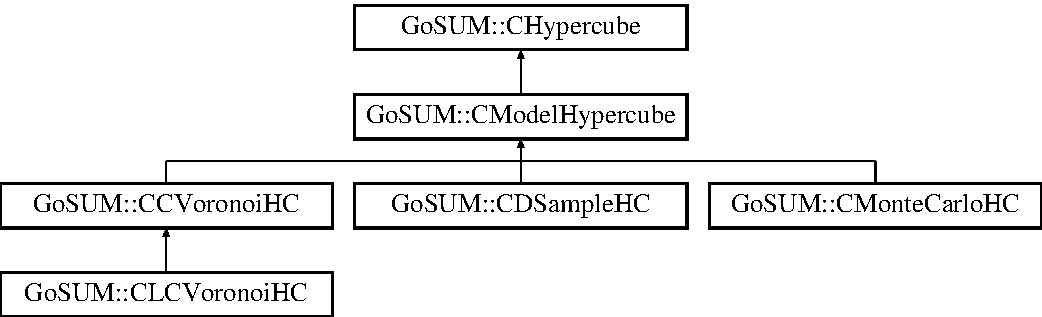
\includegraphics[height=4.000000cm]{class_go_s_u_m_1_1_c_hypercube}
\end{center}
\end{figure}
\subsection*{Public Types}
\begin{DoxyCompactItemize}
\item 
enum \hyperlink{class_go_s_u_m_1_1_c_hypercube_a9113655515864c06ea6d4f08d5195c90}{hctype} \{ \hyperlink{class_go_s_u_m_1_1_c_hypercube_a9113655515864c06ea6d4f08d5195c90abe62aed07dcbdbeda5783e3345005e16}{dsample}, 
\hyperlink{class_go_s_u_m_1_1_c_hypercube_a9113655515864c06ea6d4f08d5195c90af9afda139c9899e40caa1661dee6d2a2}{montecarlo}, 
\hyperlink{class_go_s_u_m_1_1_c_hypercube_a9113655515864c06ea6d4f08d5195c90aa7aa76eb38939f209c50edb0c5ecd16f}{cvoronoi}, 
\hyperlink{class_go_s_u_m_1_1_c_hypercube_a9113655515864c06ea6d4f08d5195c90aa292c11539b19d2d7845af56abbd1460}{lcvoronoi}
 \}
\end{DoxyCompactItemize}
\subsection*{Public Member Functions}
\begin{DoxyCompactItemize}
\item 
\hyperlink{class_go_s_u_m_1_1_c_hypercube_ab10b56e929fd581467fac4bf8d141993}{C\-Hypercube} ()
\item 
virtual \hyperlink{class_go_s_u_m_1_1_c_hypercube_af040de408525be03112bbd560768a373}{$\sim$\-C\-Hypercube} ()
\end{DoxyCompactItemize}
\subsection*{Static Public Member Functions}
\begin{DoxyCompactItemize}
\item 
static \hyperlink{class_go_s_u_m_1_1_c_hypercube_a9113655515864c06ea6d4f08d5195c90}{hctype} \hyperlink{class_go_s_u_m_1_1_c_hypercube_a6d05fe2a4610d87af24ec6b39b8e1025}{Type} (const std\-::string \&\-\_\-stype)
\begin{DoxyCompactList}\small\item\em Returns hypercube type enumerator from hypercube type name. \end{DoxyCompactList}\item 
static \hyperlink{class_go_s_u_m_1_1_c_hypercube_a9113655515864c06ea6d4f08d5195c90}{hctype} \hyperlink{class_go_s_u_m_1_1_c_hypercube_abc5b419f9502e45cb89812a08d8a41cc}{Type} ()
\begin{DoxyCompactList}\small\item\em Returns hypercube type. \end{DoxyCompactList}\item 
static void \hyperlink{class_go_s_u_m_1_1_c_hypercube_a96309f61dce90f72da0b1ecc5c3d758b}{Set\-Type} (\hyperlink{class_go_s_u_m_1_1_c_hypercube_a9113655515864c06ea6d4f08d5195c90}{hctype} \-\_\-etype)
\begin{DoxyCompactList}\small\item\em Sets hypercube type. \end{DoxyCompactList}\item 
static void \hyperlink{class_go_s_u_m_1_1_c_hypercube_a1ba153b23eaf17f51cd0b3e85f2cc59d}{Voronoi\-Options} (int \&\-\_\-maxiter, int \&\-\_\-q, double \&\-\_\-alpha2, double \&\-\_\-beta2)
\item 
static void \hyperlink{class_go_s_u_m_1_1_c_hypercube_a1c4d81419562b324b8c3486f36ef2033}{Set\-Voronoi\-Options} (int \-\_\-maxiter, int \-\_\-q, double \-\_\-alpha2, double \-\_\-beta2)
\item 
static int \hyperlink{class_go_s_u_m_1_1_c_hypercube_a402c5b23d7bb6a209ad7c423b7469008}{Cvt\-Iteration\-Size} ()
\begin{DoxyCompactList}\small\item\em Returns C\-V\-T iteration size. \end{DoxyCompactList}\item 
static void \hyperlink{class_go_s_u_m_1_1_c_hypercube_a94f1eb472623fd241372562607e8d6a5}{Set\-Cvt\-Iteration\-Size} (int \-\_\-maxiter)
\begin{DoxyCompactList}\small\item\em Sets C\-V\-T iteration size. \end{DoxyCompactList}\item 
static int \hyperlink{class_go_s_u_m_1_1_c_hypercube_acc500fc5157c78d0d1d260a502c34288}{Cvt\-Points\-Size} ()
\begin{DoxyCompactList}\small\item\em Returns C\-V\-T points size. \end{DoxyCompactList}\item 
static void \hyperlink{class_go_s_u_m_1_1_c_hypercube_a3c9ed7e8c464c78afc0eb4cf62438df9}{Set\-Cvt\-Points\-Size} (int \-\_\-q)
\begin{DoxyCompactList}\small\item\em Sets C\-V\-T points size. \end{DoxyCompactList}\item 
static double \hyperlink{class_go_s_u_m_1_1_c_hypercube_aaa4c700e7636bc8f8c627f900925af30}{Cvt\-Old\-Center\-Coefficient} ()
\begin{DoxyCompactList}\small\item\em Returns C\-V\-T parameter \#1. \end{DoxyCompactList}\item 
static void \hyperlink{class_go_s_u_m_1_1_c_hypercube_a27859b27c8e541cd42ac0424d7117b88}{Set\-Cvt\-Old\-Center\-Coefficient} (double \-\_\-alpha2)
\begin{DoxyCompactList}\small\item\em Sets C\-V\-T paramter \#1. \end{DoxyCompactList}\item 
static double \hyperlink{class_go_s_u_m_1_1_c_hypercube_a7af9011cef9d24170f558d601307a4f0}{Cvt\-New\-Center\-Coefficient} ()
\begin{DoxyCompactList}\small\item\em Returns C\-V\-T paramter \#2. \end{DoxyCompactList}\item 
static void \hyperlink{class_go_s_u_m_1_1_c_hypercube_a7347f28cd7134c3215ba0fe0c44d65e7}{Set\-Cvt\-New\-Center\-Coefficient} (double \-\_\-beta2)
\begin{DoxyCompactList}\small\item\em Sets C\-V\-T paramter \#2. \end{DoxyCompactList}\item 
static \hyperlink{class_go_s_u_m_1_1_c_model_hypercube}{Go\-S\-U\-M\-::\-C\-Model\-Hypercube} $\ast$ \hyperlink{class_go_s_u_m_1_1_c_hypercube_a737402ef325701acaf51e3a5af5f78df}{New} (\hyperlink{class_go_s_u_m_1_1_c_input_parameters}{C\-Input\-Parameters} $\ast$\-\_\-p\-I\-P)
\begin{DoxyCompactList}\small\item\em Returns new model hypercube. \end{DoxyCompactList}\item 
static int \hyperlink{class_go_s_u_m_1_1_c_hypercube_ada2117043dce22d1d0caf9f9635d7018}{Progress\-Size} (int \-\_\-rssize, int \-\_\-dim)
\begin{DoxyCompactList}\small\item\em Returns progress steps size. \end{DoxyCompactList}\end{DoxyCompactItemize}
\subsection*{Public Attributes}
\begin{DoxyCompactItemize}
\item 
boost\-::signal$<$ void()$>$ \hyperlink{class_go_s_u_m_1_1_c_hypercube_aae23731c5d5e5faf5881fc7c28542656}{generating\-Progressed}
\begin{DoxyCompactList}\small\item\em Signal for centralize progress. \end{DoxyCompactList}\end{DoxyCompactItemize}
\subsection*{Protected Member Functions}
\begin{DoxyCompactItemize}
\item 
{\footnotesize template$<$class Archive $>$ }\\void \hyperlink{class_go_s_u_m_1_1_c_hypercube_a7303a209b69f0d628b8d2249867e9247}{serialize} (Archive \&ar, const unsigned int version)
\end{DoxyCompactItemize}
\subsection*{Static Protected Attributes}
\begin{DoxyCompactItemize}
\item 
static \hyperlink{class_go_s_u_m_1_1_c_hypercube_a9113655515864c06ea6d4f08d5195c90}{hctype} \hyperlink{class_go_s_u_m_1_1_c_hypercube_a8f9d864e2940c4982480ea394931fcf5}{etype} = \hyperlink{class_go_s_u_m_1_1_c_hypercube_a9113655515864c06ea6d4f08d5195c90abe62aed07dcbdbeda5783e3345005e16}{Go\-S\-U\-M\-::\-C\-Hypercube\-::dsample}
\begin{DoxyCompactList}\small\item\em Holds hypercube type. \end{DoxyCompactList}\item 
static int \hyperlink{class_go_s_u_m_1_1_c_hypercube_a0e3ec089584a2c55fbc8db58b1e543ac}{maxiter} = 10000
\item 
static int \hyperlink{class_go_s_u_m_1_1_c_hypercube_aecbeeb5c680a49beeebbc613242055d4}{q} = 1
\begin{DoxyCompactList}\small\item\em Holds C\-V\-T parameters. \end{DoxyCompactList}\item 
static double \hyperlink{class_go_s_u_m_1_1_c_hypercube_a88f945378fe038456780cdc88aeaadd0}{alpha2} = 0.
\item 
static double \hyperlink{class_go_s_u_m_1_1_c_hypercube_a674776d76c1fd0d53a25975b057198f9}{beta2} = 1.
\end{DoxyCompactItemize}
\subsection*{Friends}
\begin{DoxyCompactItemize}
\item 
class \hyperlink{class_go_s_u_m_1_1_c_hypercube_ac98d07dd8f7b70e16ccb9a01abf56b9c}{boost\-::serialization\-::access}
\begin{DoxyCompactList}\small\item\em Boost serialization. \end{DoxyCompactList}\end{DoxyCompactItemize}


\subsection{Member Enumeration Documentation}
\hypertarget{class_go_s_u_m_1_1_c_hypercube_a9113655515864c06ea6d4f08d5195c90}{\index{Go\-S\-U\-M\-::\-C\-Hypercube@{Go\-S\-U\-M\-::\-C\-Hypercube}!hctype@{hctype}}
\index{hctype@{hctype}!GoSUM::CHypercube@{Go\-S\-U\-M\-::\-C\-Hypercube}}
\subsubsection[{hctype}]{\setlength{\rightskip}{0pt plus 5cm}enum {\bf Go\-S\-U\-M\-::\-C\-Hypercube\-::hctype}}}\label{class_go_s_u_m_1_1_c_hypercube_a9113655515864c06ea6d4f08d5195c90}
\begin{Desc}
\item[Enumerator\-: ]\par
\begin{description}
\index{dsample@{dsample}!Go\-S\-U\-M\-::\-C\-Hypercube@{Go\-S\-U\-M\-::\-C\-Hypercube}}\index{Go\-S\-U\-M\-::\-C\-Hypercube@{Go\-S\-U\-M\-::\-C\-Hypercube}!dsample@{dsample}}\item[{\em 
\hypertarget{class_go_s_u_m_1_1_c_hypercube_a9113655515864c06ea6d4f08d5195c90abe62aed07dcbdbeda5783e3345005e16}{dsample}\label{class_go_s_u_m_1_1_c_hypercube_a9113655515864c06ea6d4f08d5195c90abe62aed07dcbdbeda5783e3345005e16}
}]\index{montecarlo@{montecarlo}!Go\-S\-U\-M\-::\-C\-Hypercube@{Go\-S\-U\-M\-::\-C\-Hypercube}}\index{Go\-S\-U\-M\-::\-C\-Hypercube@{Go\-S\-U\-M\-::\-C\-Hypercube}!montecarlo@{montecarlo}}\item[{\em 
\hypertarget{class_go_s_u_m_1_1_c_hypercube_a9113655515864c06ea6d4f08d5195c90af9afda139c9899e40caa1661dee6d2a2}{montecarlo}\label{class_go_s_u_m_1_1_c_hypercube_a9113655515864c06ea6d4f08d5195c90af9afda139c9899e40caa1661dee6d2a2}
}]\index{cvoronoi@{cvoronoi}!Go\-S\-U\-M\-::\-C\-Hypercube@{Go\-S\-U\-M\-::\-C\-Hypercube}}\index{Go\-S\-U\-M\-::\-C\-Hypercube@{Go\-S\-U\-M\-::\-C\-Hypercube}!cvoronoi@{cvoronoi}}\item[{\em 
\hypertarget{class_go_s_u_m_1_1_c_hypercube_a9113655515864c06ea6d4f08d5195c90aa7aa76eb38939f209c50edb0c5ecd16f}{cvoronoi}\label{class_go_s_u_m_1_1_c_hypercube_a9113655515864c06ea6d4f08d5195c90aa7aa76eb38939f209c50edb0c5ecd16f}
}]\index{lcvoronoi@{lcvoronoi}!Go\-S\-U\-M\-::\-C\-Hypercube@{Go\-S\-U\-M\-::\-C\-Hypercube}}\index{Go\-S\-U\-M\-::\-C\-Hypercube@{Go\-S\-U\-M\-::\-C\-Hypercube}!lcvoronoi@{lcvoronoi}}\item[{\em 
\hypertarget{class_go_s_u_m_1_1_c_hypercube_a9113655515864c06ea6d4f08d5195c90aa292c11539b19d2d7845af56abbd1460}{lcvoronoi}\label{class_go_s_u_m_1_1_c_hypercube_a9113655515864c06ea6d4f08d5195c90aa292c11539b19d2d7845af56abbd1460}
}]\end{description}
\end{Desc}



\subsection{Constructor \& Destructor Documentation}
\hypertarget{class_go_s_u_m_1_1_c_hypercube_ab10b56e929fd581467fac4bf8d141993}{\index{Go\-S\-U\-M\-::\-C\-Hypercube@{Go\-S\-U\-M\-::\-C\-Hypercube}!C\-Hypercube@{C\-Hypercube}}
\index{C\-Hypercube@{C\-Hypercube}!GoSUM::CHypercube@{Go\-S\-U\-M\-::\-C\-Hypercube}}
\subsubsection[{C\-Hypercube}]{\setlength{\rightskip}{0pt plus 5cm}Go\-S\-U\-M\-::\-C\-Hypercube\-::\-C\-Hypercube (
\begin{DoxyParamCaption}
{}
\end{DoxyParamCaption}
)\hspace{0.3cm}{\ttfamily [inline]}}}\label{class_go_s_u_m_1_1_c_hypercube_ab10b56e929fd581467fac4bf8d141993}
\hypertarget{class_go_s_u_m_1_1_c_hypercube_af040de408525be03112bbd560768a373}{\index{Go\-S\-U\-M\-::\-C\-Hypercube@{Go\-S\-U\-M\-::\-C\-Hypercube}!$\sim$\-C\-Hypercube@{$\sim$\-C\-Hypercube}}
\index{$\sim$\-C\-Hypercube@{$\sim$\-C\-Hypercube}!GoSUM::CHypercube@{Go\-S\-U\-M\-::\-C\-Hypercube}}
\subsubsection[{$\sim$\-C\-Hypercube}]{\setlength{\rightskip}{0pt plus 5cm}virtual Go\-S\-U\-M\-::\-C\-Hypercube\-::$\sim$\-C\-Hypercube (
\begin{DoxyParamCaption}
{}
\end{DoxyParamCaption}
)\hspace{0.3cm}{\ttfamily [inline]}, {\ttfamily [virtual]}}}\label{class_go_s_u_m_1_1_c_hypercube_af040de408525be03112bbd560768a373}


\subsection{Member Function Documentation}
\hypertarget{class_go_s_u_m_1_1_c_hypercube_a402c5b23d7bb6a209ad7c423b7469008}{\index{Go\-S\-U\-M\-::\-C\-Hypercube@{Go\-S\-U\-M\-::\-C\-Hypercube}!Cvt\-Iteration\-Size@{Cvt\-Iteration\-Size}}
\index{Cvt\-Iteration\-Size@{Cvt\-Iteration\-Size}!GoSUM::CHypercube@{Go\-S\-U\-M\-::\-C\-Hypercube}}
\subsubsection[{Cvt\-Iteration\-Size}]{\setlength{\rightskip}{0pt plus 5cm}static int Go\-S\-U\-M\-::\-C\-Hypercube\-::\-Cvt\-Iteration\-Size (
\begin{DoxyParamCaption}
{}
\end{DoxyParamCaption}
)\hspace{0.3cm}{\ttfamily [inline]}, {\ttfamily [static]}}}\label{class_go_s_u_m_1_1_c_hypercube_a402c5b23d7bb6a209ad7c423b7469008}


Returns C\-V\-T iteration size. 

\hypertarget{class_go_s_u_m_1_1_c_hypercube_a7af9011cef9d24170f558d601307a4f0}{\index{Go\-S\-U\-M\-::\-C\-Hypercube@{Go\-S\-U\-M\-::\-C\-Hypercube}!Cvt\-New\-Center\-Coefficient@{Cvt\-New\-Center\-Coefficient}}
\index{Cvt\-New\-Center\-Coefficient@{Cvt\-New\-Center\-Coefficient}!GoSUM::CHypercube@{Go\-S\-U\-M\-::\-C\-Hypercube}}
\subsubsection[{Cvt\-New\-Center\-Coefficient}]{\setlength{\rightskip}{0pt plus 5cm}static double Go\-S\-U\-M\-::\-C\-Hypercube\-::\-Cvt\-New\-Center\-Coefficient (
\begin{DoxyParamCaption}
{}
\end{DoxyParamCaption}
)\hspace{0.3cm}{\ttfamily [inline]}, {\ttfamily [static]}}}\label{class_go_s_u_m_1_1_c_hypercube_a7af9011cef9d24170f558d601307a4f0}


Returns C\-V\-T paramter \#2. 

\hypertarget{class_go_s_u_m_1_1_c_hypercube_aaa4c700e7636bc8f8c627f900925af30}{\index{Go\-S\-U\-M\-::\-C\-Hypercube@{Go\-S\-U\-M\-::\-C\-Hypercube}!Cvt\-Old\-Center\-Coefficient@{Cvt\-Old\-Center\-Coefficient}}
\index{Cvt\-Old\-Center\-Coefficient@{Cvt\-Old\-Center\-Coefficient}!GoSUM::CHypercube@{Go\-S\-U\-M\-::\-C\-Hypercube}}
\subsubsection[{Cvt\-Old\-Center\-Coefficient}]{\setlength{\rightskip}{0pt plus 5cm}static double Go\-S\-U\-M\-::\-C\-Hypercube\-::\-Cvt\-Old\-Center\-Coefficient (
\begin{DoxyParamCaption}
{}
\end{DoxyParamCaption}
)\hspace{0.3cm}{\ttfamily [inline]}, {\ttfamily [static]}}}\label{class_go_s_u_m_1_1_c_hypercube_aaa4c700e7636bc8f8c627f900925af30}


Returns C\-V\-T parameter \#1. 

\hypertarget{class_go_s_u_m_1_1_c_hypercube_acc500fc5157c78d0d1d260a502c34288}{\index{Go\-S\-U\-M\-::\-C\-Hypercube@{Go\-S\-U\-M\-::\-C\-Hypercube}!Cvt\-Points\-Size@{Cvt\-Points\-Size}}
\index{Cvt\-Points\-Size@{Cvt\-Points\-Size}!GoSUM::CHypercube@{Go\-S\-U\-M\-::\-C\-Hypercube}}
\subsubsection[{Cvt\-Points\-Size}]{\setlength{\rightskip}{0pt plus 5cm}static int Go\-S\-U\-M\-::\-C\-Hypercube\-::\-Cvt\-Points\-Size (
\begin{DoxyParamCaption}
{}
\end{DoxyParamCaption}
)\hspace{0.3cm}{\ttfamily [inline]}, {\ttfamily [static]}}}\label{class_go_s_u_m_1_1_c_hypercube_acc500fc5157c78d0d1d260a502c34288}


Returns C\-V\-T points size. 

\hypertarget{class_go_s_u_m_1_1_c_hypercube_a737402ef325701acaf51e3a5af5f78df}{\index{Go\-S\-U\-M\-::\-C\-Hypercube@{Go\-S\-U\-M\-::\-C\-Hypercube}!New@{New}}
\index{New@{New}!GoSUM::CHypercube@{Go\-S\-U\-M\-::\-C\-Hypercube}}
\subsubsection[{New}]{\setlength{\rightskip}{0pt plus 5cm}{\bf Go\-S\-U\-M\-::\-C\-Model\-Hypercube} $\ast$ Go\-S\-U\-M\-::\-C\-Hypercube\-::\-New (
\begin{DoxyParamCaption}
\item[{{\bf C\-Input\-Parameters} $\ast$}]{\-\_\-p\-I\-P}
\end{DoxyParamCaption}
)\hspace{0.3cm}{\ttfamily [static]}}}\label{class_go_s_u_m_1_1_c_hypercube_a737402ef325701acaf51e3a5af5f78df}


Returns new model hypercube. 

\hypertarget{class_go_s_u_m_1_1_c_hypercube_ada2117043dce22d1d0caf9f9635d7018}{\index{Go\-S\-U\-M\-::\-C\-Hypercube@{Go\-S\-U\-M\-::\-C\-Hypercube}!Progress\-Size@{Progress\-Size}}
\index{Progress\-Size@{Progress\-Size}!GoSUM::CHypercube@{Go\-S\-U\-M\-::\-C\-Hypercube}}
\subsubsection[{Progress\-Size}]{\setlength{\rightskip}{0pt plus 5cm}int Go\-S\-U\-M\-::\-C\-Hypercube\-::\-Progress\-Size (
\begin{DoxyParamCaption}
\item[{int}]{\-\_\-rssize, }
\item[{int}]{\-\_\-dim}
\end{DoxyParamCaption}
)\hspace{0.3cm}{\ttfamily [static]}}}\label{class_go_s_u_m_1_1_c_hypercube_ada2117043dce22d1d0caf9f9635d7018}


Returns progress steps size. 

\hypertarget{class_go_s_u_m_1_1_c_hypercube_a7303a209b69f0d628b8d2249867e9247}{\index{Go\-S\-U\-M\-::\-C\-Hypercube@{Go\-S\-U\-M\-::\-C\-Hypercube}!serialize@{serialize}}
\index{serialize@{serialize}!GoSUM::CHypercube@{Go\-S\-U\-M\-::\-C\-Hypercube}}
\subsubsection[{serialize}]{\setlength{\rightskip}{0pt plus 5cm}template$<$class Archive $>$ void Go\-S\-U\-M\-::\-C\-Hypercube\-::serialize (
\begin{DoxyParamCaption}
\item[{Archive \&}]{ar, }
\item[{const unsigned int}]{version}
\end{DoxyParamCaption}
)\hspace{0.3cm}{\ttfamily [protected]}}}\label{class_go_s_u_m_1_1_c_hypercube_a7303a209b69f0d628b8d2249867e9247}


Reimplemented in \hyperlink{class_go_s_u_m_1_1_c_l_c_voronoi_h_c_a98f588c33a8f2e2f4b681b48d63f2109}{Go\-S\-U\-M\-::\-C\-L\-C\-Voronoi\-H\-C}, \hyperlink{class_go_s_u_m_1_1_c_c_voronoi_h_c_abbeaabd93028069b81be4dfc078e3d02}{Go\-S\-U\-M\-::\-C\-C\-Voronoi\-H\-C}, \hyperlink{class_go_s_u_m_1_1_c_monte_carlo_h_c_ae04ab348b02072028893eee2541cadf8}{Go\-S\-U\-M\-::\-C\-Monte\-Carlo\-H\-C}, and \hyperlink{class_go_s_u_m_1_1_c_model_hypercube_a67de6632c6f6ca3685d2a750599974c6}{Go\-S\-U\-M\-::\-C\-Model\-Hypercube}.

\hypertarget{class_go_s_u_m_1_1_c_hypercube_a94f1eb472623fd241372562607e8d6a5}{\index{Go\-S\-U\-M\-::\-C\-Hypercube@{Go\-S\-U\-M\-::\-C\-Hypercube}!Set\-Cvt\-Iteration\-Size@{Set\-Cvt\-Iteration\-Size}}
\index{Set\-Cvt\-Iteration\-Size@{Set\-Cvt\-Iteration\-Size}!GoSUM::CHypercube@{Go\-S\-U\-M\-::\-C\-Hypercube}}
\subsubsection[{Set\-Cvt\-Iteration\-Size}]{\setlength{\rightskip}{0pt plus 5cm}static void Go\-S\-U\-M\-::\-C\-Hypercube\-::\-Set\-Cvt\-Iteration\-Size (
\begin{DoxyParamCaption}
\item[{int}]{\-\_\-maxiter}
\end{DoxyParamCaption}
)\hspace{0.3cm}{\ttfamily [inline]}, {\ttfamily [static]}}}\label{class_go_s_u_m_1_1_c_hypercube_a94f1eb472623fd241372562607e8d6a5}


Sets C\-V\-T iteration size. 

\hypertarget{class_go_s_u_m_1_1_c_hypercube_a7347f28cd7134c3215ba0fe0c44d65e7}{\index{Go\-S\-U\-M\-::\-C\-Hypercube@{Go\-S\-U\-M\-::\-C\-Hypercube}!Set\-Cvt\-New\-Center\-Coefficient@{Set\-Cvt\-New\-Center\-Coefficient}}
\index{Set\-Cvt\-New\-Center\-Coefficient@{Set\-Cvt\-New\-Center\-Coefficient}!GoSUM::CHypercube@{Go\-S\-U\-M\-::\-C\-Hypercube}}
\subsubsection[{Set\-Cvt\-New\-Center\-Coefficient}]{\setlength{\rightskip}{0pt plus 5cm}static void Go\-S\-U\-M\-::\-C\-Hypercube\-::\-Set\-Cvt\-New\-Center\-Coefficient (
\begin{DoxyParamCaption}
\item[{double}]{\-\_\-beta2}
\end{DoxyParamCaption}
)\hspace{0.3cm}{\ttfamily [inline]}, {\ttfamily [static]}}}\label{class_go_s_u_m_1_1_c_hypercube_a7347f28cd7134c3215ba0fe0c44d65e7}


Sets C\-V\-T paramter \#2. 

\hypertarget{class_go_s_u_m_1_1_c_hypercube_a27859b27c8e541cd42ac0424d7117b88}{\index{Go\-S\-U\-M\-::\-C\-Hypercube@{Go\-S\-U\-M\-::\-C\-Hypercube}!Set\-Cvt\-Old\-Center\-Coefficient@{Set\-Cvt\-Old\-Center\-Coefficient}}
\index{Set\-Cvt\-Old\-Center\-Coefficient@{Set\-Cvt\-Old\-Center\-Coefficient}!GoSUM::CHypercube@{Go\-S\-U\-M\-::\-C\-Hypercube}}
\subsubsection[{Set\-Cvt\-Old\-Center\-Coefficient}]{\setlength{\rightskip}{0pt plus 5cm}static void Go\-S\-U\-M\-::\-C\-Hypercube\-::\-Set\-Cvt\-Old\-Center\-Coefficient (
\begin{DoxyParamCaption}
\item[{double}]{\-\_\-alpha2}
\end{DoxyParamCaption}
)\hspace{0.3cm}{\ttfamily [inline]}, {\ttfamily [static]}}}\label{class_go_s_u_m_1_1_c_hypercube_a27859b27c8e541cd42ac0424d7117b88}


Sets C\-V\-T paramter \#1. 

\hypertarget{class_go_s_u_m_1_1_c_hypercube_a3c9ed7e8c464c78afc0eb4cf62438df9}{\index{Go\-S\-U\-M\-::\-C\-Hypercube@{Go\-S\-U\-M\-::\-C\-Hypercube}!Set\-Cvt\-Points\-Size@{Set\-Cvt\-Points\-Size}}
\index{Set\-Cvt\-Points\-Size@{Set\-Cvt\-Points\-Size}!GoSUM::CHypercube@{Go\-S\-U\-M\-::\-C\-Hypercube}}
\subsubsection[{Set\-Cvt\-Points\-Size}]{\setlength{\rightskip}{0pt plus 5cm}static void Go\-S\-U\-M\-::\-C\-Hypercube\-::\-Set\-Cvt\-Points\-Size (
\begin{DoxyParamCaption}
\item[{int}]{\-\_\-q}
\end{DoxyParamCaption}
)\hspace{0.3cm}{\ttfamily [inline]}, {\ttfamily [static]}}}\label{class_go_s_u_m_1_1_c_hypercube_a3c9ed7e8c464c78afc0eb4cf62438df9}


Sets C\-V\-T points size. 

\hypertarget{class_go_s_u_m_1_1_c_hypercube_a96309f61dce90f72da0b1ecc5c3d758b}{\index{Go\-S\-U\-M\-::\-C\-Hypercube@{Go\-S\-U\-M\-::\-C\-Hypercube}!Set\-Type@{Set\-Type}}
\index{Set\-Type@{Set\-Type}!GoSUM::CHypercube@{Go\-S\-U\-M\-::\-C\-Hypercube}}
\subsubsection[{Set\-Type}]{\setlength{\rightskip}{0pt plus 5cm}void Go\-S\-U\-M\-::\-C\-Hypercube\-::\-Set\-Type (
\begin{DoxyParamCaption}
\item[{{\bf hctype}}]{\-\_\-etype}
\end{DoxyParamCaption}
)\hspace{0.3cm}{\ttfamily [static]}}}\label{class_go_s_u_m_1_1_c_hypercube_a96309f61dce90f72da0b1ecc5c3d758b}


Sets hypercube type. 

\hypertarget{class_go_s_u_m_1_1_c_hypercube_a1c4d81419562b324b8c3486f36ef2033}{\index{Go\-S\-U\-M\-::\-C\-Hypercube@{Go\-S\-U\-M\-::\-C\-Hypercube}!Set\-Voronoi\-Options@{Set\-Voronoi\-Options}}
\index{Set\-Voronoi\-Options@{Set\-Voronoi\-Options}!GoSUM::CHypercube@{Go\-S\-U\-M\-::\-C\-Hypercube}}
\subsubsection[{Set\-Voronoi\-Options}]{\setlength{\rightskip}{0pt plus 5cm}static void Go\-S\-U\-M\-::\-C\-Hypercube\-::\-Set\-Voronoi\-Options (
\begin{DoxyParamCaption}
\item[{int}]{\-\_\-maxiter, }
\item[{int}]{\-\_\-q, }
\item[{double}]{\-\_\-alpha2, }
\item[{double}]{\-\_\-beta2}
\end{DoxyParamCaption}
)\hspace{0.3cm}{\ttfamily [inline]}, {\ttfamily [static]}}}\label{class_go_s_u_m_1_1_c_hypercube_a1c4d81419562b324b8c3486f36ef2033}

\begin{DoxyParams}{Parameters}
{\em \-\_\-beta2} & Sets Voronoi options. \\
\hline
\end{DoxyParams}
\hypertarget{class_go_s_u_m_1_1_c_hypercube_a6d05fe2a4610d87af24ec6b39b8e1025}{\index{Go\-S\-U\-M\-::\-C\-Hypercube@{Go\-S\-U\-M\-::\-C\-Hypercube}!Type@{Type}}
\index{Type@{Type}!GoSUM::CHypercube@{Go\-S\-U\-M\-::\-C\-Hypercube}}
\subsubsection[{Type}]{\setlength{\rightskip}{0pt plus 5cm}{\bf Go\-S\-U\-M\-::\-C\-Hypercube\-::hctype} Go\-S\-U\-M\-::\-C\-Hypercube\-::\-Type (
\begin{DoxyParamCaption}
\item[{const std\-::string \&}]{\-\_\-stype}
\end{DoxyParamCaption}
)\hspace{0.3cm}{\ttfamily [static]}}}\label{class_go_s_u_m_1_1_c_hypercube_a6d05fe2a4610d87af24ec6b39b8e1025}


Returns hypercube type enumerator from hypercube type name. 

\hypertarget{class_go_s_u_m_1_1_c_hypercube_abc5b419f9502e45cb89812a08d8a41cc}{\index{Go\-S\-U\-M\-::\-C\-Hypercube@{Go\-S\-U\-M\-::\-C\-Hypercube}!Type@{Type}}
\index{Type@{Type}!GoSUM::CHypercube@{Go\-S\-U\-M\-::\-C\-Hypercube}}
\subsubsection[{Type}]{\setlength{\rightskip}{0pt plus 5cm}static {\bf hctype} Go\-S\-U\-M\-::\-C\-Hypercube\-::\-Type (
\begin{DoxyParamCaption}
{}
\end{DoxyParamCaption}
)\hspace{0.3cm}{\ttfamily [inline]}, {\ttfamily [static]}}}\label{class_go_s_u_m_1_1_c_hypercube_abc5b419f9502e45cb89812a08d8a41cc}


Returns hypercube type. 

\hypertarget{class_go_s_u_m_1_1_c_hypercube_a1ba153b23eaf17f51cd0b3e85f2cc59d}{\index{Go\-S\-U\-M\-::\-C\-Hypercube@{Go\-S\-U\-M\-::\-C\-Hypercube}!Voronoi\-Options@{Voronoi\-Options}}
\index{Voronoi\-Options@{Voronoi\-Options}!GoSUM::CHypercube@{Go\-S\-U\-M\-::\-C\-Hypercube}}
\subsubsection[{Voronoi\-Options}]{\setlength{\rightskip}{0pt plus 5cm}static void Go\-S\-U\-M\-::\-C\-Hypercube\-::\-Voronoi\-Options (
\begin{DoxyParamCaption}
\item[{int \&}]{\-\_\-maxiter, }
\item[{int \&}]{\-\_\-q, }
\item[{double \&}]{\-\_\-alpha2, }
\item[{double \&}]{\-\_\-beta2}
\end{DoxyParamCaption}
)\hspace{0.3cm}{\ttfamily [inline]}, {\ttfamily [static]}}}\label{class_go_s_u_m_1_1_c_hypercube_a1ba153b23eaf17f51cd0b3e85f2cc59d}

\begin{DoxyParams}{Parameters}
{\em \-\_\-beta2} & Returns Voronoi options. \\
\hline
\end{DoxyParams}


\subsection{Friends And Related Function Documentation}
\hypertarget{class_go_s_u_m_1_1_c_hypercube_ac98d07dd8f7b70e16ccb9a01abf56b9c}{\index{Go\-S\-U\-M\-::\-C\-Hypercube@{Go\-S\-U\-M\-::\-C\-Hypercube}!boost\-::serialization\-::access@{boost\-::serialization\-::access}}
\index{boost\-::serialization\-::access@{boost\-::serialization\-::access}!GoSUM::CHypercube@{Go\-S\-U\-M\-::\-C\-Hypercube}}
\subsubsection[{boost\-::serialization\-::access}]{\setlength{\rightskip}{0pt plus 5cm}friend class boost\-::serialization\-::access\hspace{0.3cm}{\ttfamily [friend]}}}\label{class_go_s_u_m_1_1_c_hypercube_ac98d07dd8f7b70e16ccb9a01abf56b9c}


Boost serialization. 



\subsection{Member Data Documentation}
\hypertarget{class_go_s_u_m_1_1_c_hypercube_a88f945378fe038456780cdc88aeaadd0}{\index{Go\-S\-U\-M\-::\-C\-Hypercube@{Go\-S\-U\-M\-::\-C\-Hypercube}!alpha2@{alpha2}}
\index{alpha2@{alpha2}!GoSUM::CHypercube@{Go\-S\-U\-M\-::\-C\-Hypercube}}
\subsubsection[{alpha2}]{\setlength{\rightskip}{0pt plus 5cm}double Go\-S\-U\-M\-::\-C\-Hypercube\-::alpha2 = 0.\hspace{0.3cm}{\ttfamily [static]}, {\ttfamily [protected]}}}\label{class_go_s_u_m_1_1_c_hypercube_a88f945378fe038456780cdc88aeaadd0}
\hypertarget{class_go_s_u_m_1_1_c_hypercube_a674776d76c1fd0d53a25975b057198f9}{\index{Go\-S\-U\-M\-::\-C\-Hypercube@{Go\-S\-U\-M\-::\-C\-Hypercube}!beta2@{beta2}}
\index{beta2@{beta2}!GoSUM::CHypercube@{Go\-S\-U\-M\-::\-C\-Hypercube}}
\subsubsection[{beta2}]{\setlength{\rightskip}{0pt plus 5cm}double Go\-S\-U\-M\-::\-C\-Hypercube\-::beta2 = 1.\hspace{0.3cm}{\ttfamily [static]}, {\ttfamily [protected]}}}\label{class_go_s_u_m_1_1_c_hypercube_a674776d76c1fd0d53a25975b057198f9}
Holds C\-V\-T parameters. \hypertarget{class_go_s_u_m_1_1_c_hypercube_a8f9d864e2940c4982480ea394931fcf5}{\index{Go\-S\-U\-M\-::\-C\-Hypercube@{Go\-S\-U\-M\-::\-C\-Hypercube}!etype@{etype}}
\index{etype@{etype}!GoSUM::CHypercube@{Go\-S\-U\-M\-::\-C\-Hypercube}}
\subsubsection[{etype}]{\setlength{\rightskip}{0pt plus 5cm}{\bf Go\-S\-U\-M\-::\-C\-Hypercube\-::hctype} Go\-S\-U\-M\-::\-C\-Hypercube\-::etype = {\bf Go\-S\-U\-M\-::\-C\-Hypercube\-::dsample}\hspace{0.3cm}{\ttfamily [static]}, {\ttfamily [protected]}}}\label{class_go_s_u_m_1_1_c_hypercube_a8f9d864e2940c4982480ea394931fcf5}


Holds hypercube type. 

\hypertarget{class_go_s_u_m_1_1_c_hypercube_aae23731c5d5e5faf5881fc7c28542656}{\index{Go\-S\-U\-M\-::\-C\-Hypercube@{Go\-S\-U\-M\-::\-C\-Hypercube}!generating\-Progressed@{generating\-Progressed}}
\index{generating\-Progressed@{generating\-Progressed}!GoSUM::CHypercube@{Go\-S\-U\-M\-::\-C\-Hypercube}}
\subsubsection[{generating\-Progressed}]{\setlength{\rightskip}{0pt plus 5cm}boost\-::signal$<$void()$>$ Go\-S\-U\-M\-::\-C\-Hypercube\-::generating\-Progressed}}\label{class_go_s_u_m_1_1_c_hypercube_aae23731c5d5e5faf5881fc7c28542656}


Signal for centralize progress. 

\hypertarget{class_go_s_u_m_1_1_c_hypercube_a0e3ec089584a2c55fbc8db58b1e543ac}{\index{Go\-S\-U\-M\-::\-C\-Hypercube@{Go\-S\-U\-M\-::\-C\-Hypercube}!maxiter@{maxiter}}
\index{maxiter@{maxiter}!GoSUM::CHypercube@{Go\-S\-U\-M\-::\-C\-Hypercube}}
\subsubsection[{maxiter}]{\setlength{\rightskip}{0pt plus 5cm}int Go\-S\-U\-M\-::\-C\-Hypercube\-::maxiter = 10000\hspace{0.3cm}{\ttfamily [static]}, {\ttfamily [protected]}}}\label{class_go_s_u_m_1_1_c_hypercube_a0e3ec089584a2c55fbc8db58b1e543ac}
\hypertarget{class_go_s_u_m_1_1_c_hypercube_aecbeeb5c680a49beeebbc613242055d4}{\index{Go\-S\-U\-M\-::\-C\-Hypercube@{Go\-S\-U\-M\-::\-C\-Hypercube}!q@{q}}
\index{q@{q}!GoSUM::CHypercube@{Go\-S\-U\-M\-::\-C\-Hypercube}}
\subsubsection[{q}]{\setlength{\rightskip}{0pt plus 5cm}int Go\-S\-U\-M\-::\-C\-Hypercube\-::q = 1\hspace{0.3cm}{\ttfamily [static]}, {\ttfamily [protected]}}}\label{class_go_s_u_m_1_1_c_hypercube_aecbeeb5c680a49beeebbc613242055d4}


Holds C\-V\-T parameters. 



The documentation for this class was generated from the following files\-:\begin{DoxyCompactItemize}
\item 
C\-:/\-Development/core/\hyperlink{_hypercube_8h}{Hypercube.\-h}\item 
C\-:/\-Development/core/\hyperlink{_hypercube_8cpp}{Hypercube.\-cpp}\end{DoxyCompactItemize}

\hypertarget{class_go_s_u_m_1_1_c_input_parameters}{\section{Go\-S\-U\-M\-:\-:C\-Input\-Parameters Class Reference}
\label{class_go_s_u_m_1_1_c_input_parameters}\index{Go\-S\-U\-M\-::\-C\-Input\-Parameters@{Go\-S\-U\-M\-::\-C\-Input\-Parameters}}
}


Class for \hyperlink{struct_go_s_u_m}{Go\-S\-U\-M} input parameters.  




{\ttfamily \#include $<$Model.\-h$>$}

Inheritance diagram for Go\-S\-U\-M\-:\-:C\-Input\-Parameters\-:\begin{figure}[H]
\begin{center}
\leavevmode
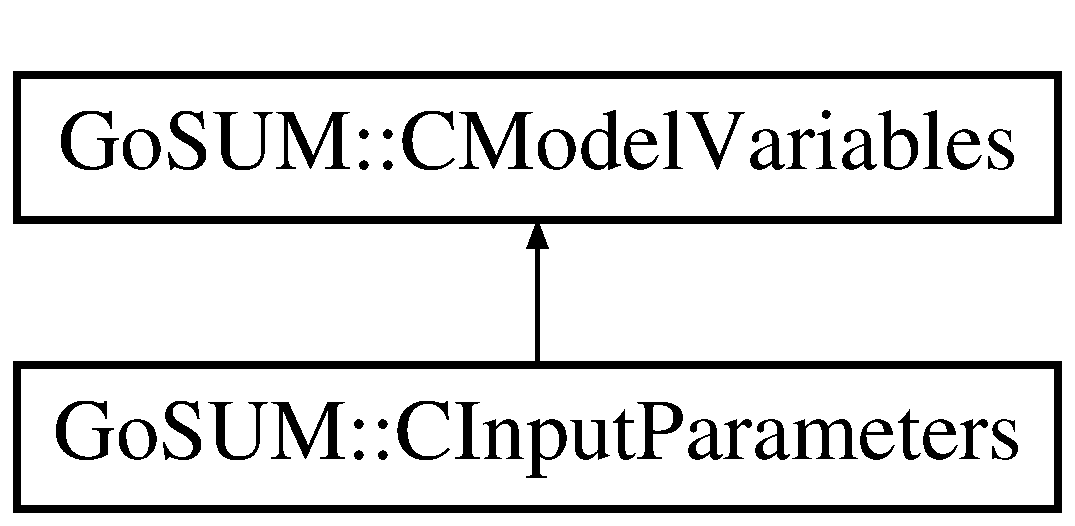
\includegraphics[height=2.000000cm]{class_go_s_u_m_1_1_c_input_parameters}
\end{center}
\end{figure}
\subsection*{Public Member Functions}
\begin{DoxyCompactItemize}
\item 
\hyperlink{class_go_s_u_m_1_1_c_input_parameters_a1d2c088e6335ce2ff4b10ff5964cb9b9}{C\-Input\-Parameters} (\hyperlink{class_go_s_u_m_1_1_c_model_constraints}{C\-Model\-Constraints} $\ast$\-\_\-p\-I\-C)
\item 
virtual \hyperlink{class_go_s_u_m_1_1_c_input_parameters_ac9d5bfe8ecf12ccc78dc1327b4d4765d}{$\sim$\-C\-Input\-Parameters} ()
\item 
int \hyperlink{class_go_s_u_m_1_1_c_input_parameters_a7d9e6f3799e28997cc1b3d1071804eda}{resample\-Size} () const 
\begin{DoxyCompactList}\small\item\em Returns resampling size. \end{DoxyCompactList}\item 
void \hyperlink{class_go_s_u_m_1_1_c_input_parameters_a7be5d110240bdd04b150cd7e511837fc}{set\-Resample\-Size} (int \-\_\-\-R\-Ssize)
\begin{DoxyCompactList}\small\item\em Sets resampling size. \end{DoxyCompactList}\item 
void \hyperlink{class_go_s_u_m_1_1_c_input_parameters_a1bb1435964c789f0cfa311e78d165ed8}{generate\-Samples} (std\-::vector$<$ Array\-Xd $>$ \&\-\_\-samples)
\begin{DoxyCompactList}\small\item\em Generates samples on external vector of samples. \end{DoxyCompactList}\item 
void \hyperlink{class_go_s_u_m_1_1_c_input_parameters_a63b7df5e450248ad37f9ac17adb0373b}{generate\-Samples} ()
\begin{DoxyCompactList}\small\item\em Generates samples on internal model variable samples. \end{DoxyCompactList}\item 
int \hyperlink{class_go_s_u_m_1_1_c_input_parameters_a3bd69f7c2974ffba079630fcc1502e38}{resample\-Steps\-Size} () const 
\begin{DoxyCompactList}\small\item\em Returns resample steps size. \end{DoxyCompactList}\item 
\hyperlink{class_go_s_u_m_1_1_c_model_constraints}{C\-Model\-Constraints} $\ast$ \hyperlink{class_go_s_u_m_1_1_c_input_parameters_af672bb23aae739eb3030bd25dcacc082}{constraints} () const 
\begin{DoxyCompactList}\small\item\em Returns pointer to model constraints. \end{DoxyCompactList}\item 
void \hyperlink{class_go_s_u_m_1_1_c_input_parameters_a13ef77936322f7adce5f44ce2793fc42}{set\-Progress\-Slot} (boost\-::function$<$ void()$>$ \-\_\-progress\-Slot)
\begin{DoxyCompactList}\small\item\em Sets external progress slot. \end{DoxyCompactList}\end{DoxyCompactItemize}
\subsection*{Public Attributes}
\begin{DoxyCompactItemize}
\item 
boost\-::function$<$ void()$>$ \hyperlink{class_go_s_u_m_1_1_c_input_parameters_a7b08f28eae560f682cacb13647cd75ac}{progress\-Slot}
\begin{DoxyCompactList}\small\item\em External progress slot, later connected to signal for evalaution progress. \end{DoxyCompactList}\end{DoxyCompactItemize}
\subsection*{Private Member Functions}
\begin{DoxyCompactItemize}
\item 
{\footnotesize template$<$class Archive $>$ }\\void \hyperlink{class_go_s_u_m_1_1_c_input_parameters_aeb3b6421966bee3d7d38dc6df3a17ee3}{serialize} (Archive \&ar, const unsigned int version)
\item 
\hyperlink{class_go_s_u_m_1_1_c_input_parameters_a8708f612809710de0aa03dc062249c30}{C\-Input\-Parameters} ()
\end{DoxyCompactItemize}
\subsection*{Private Attributes}
\begin{DoxyCompactItemize}
\item 
\hyperlink{class_go_s_u_m_1_1_c_model_constraints}{C\-Model\-Constraints} $\ast$ \hyperlink{class_go_s_u_m_1_1_c_input_parameters_a6ea7a2d7d1ceb033321890c5313a6595}{p\-I\-C}
\begin{DoxyCompactList}\small\item\em Points to model constraints. \end{DoxyCompactList}\item 
int \hyperlink{class_go_s_u_m_1_1_c_input_parameters_ad33f3fe5498287609093ca480c221458}{R\-Ssize}
\end{DoxyCompactItemize}
\subsection*{Friends}
\begin{DoxyCompactItemize}
\item 
class \hyperlink{class_go_s_u_m_1_1_c_input_parameters_ac98d07dd8f7b70e16ccb9a01abf56b9c}{boost\-::serialization\-::access}
\begin{DoxyCompactList}\small\item\em Boost serialization. \end{DoxyCompactList}\end{DoxyCompactItemize}
\subsection*{Additional Inherited Members}


\subsection{Detailed Description}
Class for \hyperlink{struct_go_s_u_m}{Go\-S\-U\-M} input parameters. 

\subsection{Constructor \& Destructor Documentation}
\hypertarget{class_go_s_u_m_1_1_c_input_parameters_a8708f612809710de0aa03dc062249c30}{\index{Go\-S\-U\-M\-::\-C\-Input\-Parameters@{Go\-S\-U\-M\-::\-C\-Input\-Parameters}!C\-Input\-Parameters@{C\-Input\-Parameters}}
\index{C\-Input\-Parameters@{C\-Input\-Parameters}!GoSUM::CInputParameters@{Go\-S\-U\-M\-::\-C\-Input\-Parameters}}
\subsubsection[{C\-Input\-Parameters}]{\setlength{\rightskip}{0pt plus 5cm}Go\-S\-U\-M\-::\-C\-Input\-Parameters\-::\-C\-Input\-Parameters (
\begin{DoxyParamCaption}
{}
\end{DoxyParamCaption}
)\hspace{0.3cm}{\ttfamily [inline]}, {\ttfamily [private]}}}\label{class_go_s_u_m_1_1_c_input_parameters_a8708f612809710de0aa03dc062249c30}
\hypertarget{class_go_s_u_m_1_1_c_input_parameters_a1d2c088e6335ce2ff4b10ff5964cb9b9}{\index{Go\-S\-U\-M\-::\-C\-Input\-Parameters@{Go\-S\-U\-M\-::\-C\-Input\-Parameters}!C\-Input\-Parameters@{C\-Input\-Parameters}}
\index{C\-Input\-Parameters@{C\-Input\-Parameters}!GoSUM::CInputParameters@{Go\-S\-U\-M\-::\-C\-Input\-Parameters}}
\subsubsection[{C\-Input\-Parameters}]{\setlength{\rightskip}{0pt plus 5cm}Go\-S\-U\-M\-::\-C\-Input\-Parameters\-::\-C\-Input\-Parameters (
\begin{DoxyParamCaption}
\item[{{\bf C\-Model\-Constraints} $\ast$}]{\-\_\-p\-I\-C}
\end{DoxyParamCaption}
)\hspace{0.3cm}{\ttfamily [inline]}}}\label{class_go_s_u_m_1_1_c_input_parameters_a1d2c088e6335ce2ff4b10ff5964cb9b9}
\hypertarget{class_go_s_u_m_1_1_c_input_parameters_ac9d5bfe8ecf12ccc78dc1327b4d4765d}{\index{Go\-S\-U\-M\-::\-C\-Input\-Parameters@{Go\-S\-U\-M\-::\-C\-Input\-Parameters}!$\sim$\-C\-Input\-Parameters@{$\sim$\-C\-Input\-Parameters}}
\index{$\sim$\-C\-Input\-Parameters@{$\sim$\-C\-Input\-Parameters}!GoSUM::CInputParameters@{Go\-S\-U\-M\-::\-C\-Input\-Parameters}}
\subsubsection[{$\sim$\-C\-Input\-Parameters}]{\setlength{\rightskip}{0pt plus 5cm}virtual Go\-S\-U\-M\-::\-C\-Input\-Parameters\-::$\sim$\-C\-Input\-Parameters (
\begin{DoxyParamCaption}
{}
\end{DoxyParamCaption}
)\hspace{0.3cm}{\ttfamily [inline]}, {\ttfamily [virtual]}}}\label{class_go_s_u_m_1_1_c_input_parameters_ac9d5bfe8ecf12ccc78dc1327b4d4765d}


\subsection{Member Function Documentation}
\hypertarget{class_go_s_u_m_1_1_c_input_parameters_af672bb23aae739eb3030bd25dcacc082}{\index{Go\-S\-U\-M\-::\-C\-Input\-Parameters@{Go\-S\-U\-M\-::\-C\-Input\-Parameters}!constraints@{constraints}}
\index{constraints@{constraints}!GoSUM::CInputParameters@{Go\-S\-U\-M\-::\-C\-Input\-Parameters}}
\subsubsection[{constraints}]{\setlength{\rightskip}{0pt plus 5cm}{\bf C\-Model\-Constraints}$\ast$ Go\-S\-U\-M\-::\-C\-Input\-Parameters\-::constraints (
\begin{DoxyParamCaption}
{}
\end{DoxyParamCaption}
) const\hspace{0.3cm}{\ttfamily [inline]}}}\label{class_go_s_u_m_1_1_c_input_parameters_af672bb23aae739eb3030bd25dcacc082}


Returns pointer to model constraints. 

\hypertarget{class_go_s_u_m_1_1_c_input_parameters_a1bb1435964c789f0cfa311e78d165ed8}{\index{Go\-S\-U\-M\-::\-C\-Input\-Parameters@{Go\-S\-U\-M\-::\-C\-Input\-Parameters}!generate\-Samples@{generate\-Samples}}
\index{generate\-Samples@{generate\-Samples}!GoSUM::CInputParameters@{Go\-S\-U\-M\-::\-C\-Input\-Parameters}}
\subsubsection[{generate\-Samples}]{\setlength{\rightskip}{0pt plus 5cm}void Go\-S\-U\-M\-::\-C\-Input\-Parameters\-::generate\-Samples (
\begin{DoxyParamCaption}
\item[{std\-::vector$<$ Array\-Xd $>$ \&}]{\-\_\-samples}
\end{DoxyParamCaption}
)}}\label{class_go_s_u_m_1_1_c_input_parameters_a1bb1435964c789f0cfa311e78d165ed8}


Generates samples on external vector of samples. 

\hypertarget{class_go_s_u_m_1_1_c_input_parameters_a63b7df5e450248ad37f9ac17adb0373b}{\index{Go\-S\-U\-M\-::\-C\-Input\-Parameters@{Go\-S\-U\-M\-::\-C\-Input\-Parameters}!generate\-Samples@{generate\-Samples}}
\index{generate\-Samples@{generate\-Samples}!GoSUM::CInputParameters@{Go\-S\-U\-M\-::\-C\-Input\-Parameters}}
\subsubsection[{generate\-Samples}]{\setlength{\rightskip}{0pt plus 5cm}void Go\-S\-U\-M\-::\-C\-Input\-Parameters\-::generate\-Samples (
\begin{DoxyParamCaption}
{}
\end{DoxyParamCaption}
)}}\label{class_go_s_u_m_1_1_c_input_parameters_a63b7df5e450248ad37f9ac17adb0373b}


Generates samples on internal model variable samples. 

\hypertarget{class_go_s_u_m_1_1_c_input_parameters_a7d9e6f3799e28997cc1b3d1071804eda}{\index{Go\-S\-U\-M\-::\-C\-Input\-Parameters@{Go\-S\-U\-M\-::\-C\-Input\-Parameters}!resample\-Size@{resample\-Size}}
\index{resample\-Size@{resample\-Size}!GoSUM::CInputParameters@{Go\-S\-U\-M\-::\-C\-Input\-Parameters}}
\subsubsection[{resample\-Size}]{\setlength{\rightskip}{0pt plus 5cm}int Go\-S\-U\-M\-::\-C\-Input\-Parameters\-::resample\-Size (
\begin{DoxyParamCaption}
{}
\end{DoxyParamCaption}
) const\hspace{0.3cm}{\ttfamily [inline]}}}\label{class_go_s_u_m_1_1_c_input_parameters_a7d9e6f3799e28997cc1b3d1071804eda}


Returns resampling size. 

\hypertarget{class_go_s_u_m_1_1_c_input_parameters_a3bd69f7c2974ffba079630fcc1502e38}{\index{Go\-S\-U\-M\-::\-C\-Input\-Parameters@{Go\-S\-U\-M\-::\-C\-Input\-Parameters}!resample\-Steps\-Size@{resample\-Steps\-Size}}
\index{resample\-Steps\-Size@{resample\-Steps\-Size}!GoSUM::CInputParameters@{Go\-S\-U\-M\-::\-C\-Input\-Parameters}}
\subsubsection[{resample\-Steps\-Size}]{\setlength{\rightskip}{0pt plus 5cm}int Go\-S\-U\-M\-::\-C\-Input\-Parameters\-::resample\-Steps\-Size (
\begin{DoxyParamCaption}
{}
\end{DoxyParamCaption}
) const}}\label{class_go_s_u_m_1_1_c_input_parameters_a3bd69f7c2974ffba079630fcc1502e38}


Returns resample steps size. 

\hypertarget{class_go_s_u_m_1_1_c_input_parameters_aeb3b6421966bee3d7d38dc6df3a17ee3}{\index{Go\-S\-U\-M\-::\-C\-Input\-Parameters@{Go\-S\-U\-M\-::\-C\-Input\-Parameters}!serialize@{serialize}}
\index{serialize@{serialize}!GoSUM::CInputParameters@{Go\-S\-U\-M\-::\-C\-Input\-Parameters}}
\subsubsection[{serialize}]{\setlength{\rightskip}{0pt plus 5cm}template$<$class Archive $>$ void Go\-S\-U\-M\-::\-C\-Input\-Parameters\-::serialize (
\begin{DoxyParamCaption}
\item[{Archive \&}]{ar, }
\item[{const unsigned int}]{version}
\end{DoxyParamCaption}
)\hspace{0.3cm}{\ttfamily [private]}}}\label{class_go_s_u_m_1_1_c_input_parameters_aeb3b6421966bee3d7d38dc6df3a17ee3}
\hypertarget{class_go_s_u_m_1_1_c_input_parameters_a13ef77936322f7adce5f44ce2793fc42}{\index{Go\-S\-U\-M\-::\-C\-Input\-Parameters@{Go\-S\-U\-M\-::\-C\-Input\-Parameters}!set\-Progress\-Slot@{set\-Progress\-Slot}}
\index{set\-Progress\-Slot@{set\-Progress\-Slot}!GoSUM::CInputParameters@{Go\-S\-U\-M\-::\-C\-Input\-Parameters}}
\subsubsection[{set\-Progress\-Slot}]{\setlength{\rightskip}{0pt plus 5cm}void Go\-S\-U\-M\-::\-C\-Input\-Parameters\-::set\-Progress\-Slot (
\begin{DoxyParamCaption}
\item[{boost\-::function$<$ void()$>$}]{\-\_\-progress\-Slot}
\end{DoxyParamCaption}
)\hspace{0.3cm}{\ttfamily [inline]}}}\label{class_go_s_u_m_1_1_c_input_parameters_a13ef77936322f7adce5f44ce2793fc42}


Sets external progress slot. 

\hypertarget{class_go_s_u_m_1_1_c_input_parameters_a7be5d110240bdd04b150cd7e511837fc}{\index{Go\-S\-U\-M\-::\-C\-Input\-Parameters@{Go\-S\-U\-M\-::\-C\-Input\-Parameters}!set\-Resample\-Size@{set\-Resample\-Size}}
\index{set\-Resample\-Size@{set\-Resample\-Size}!GoSUM::CInputParameters@{Go\-S\-U\-M\-::\-C\-Input\-Parameters}}
\subsubsection[{set\-Resample\-Size}]{\setlength{\rightskip}{0pt plus 5cm}void Go\-S\-U\-M\-::\-C\-Input\-Parameters\-::set\-Resample\-Size (
\begin{DoxyParamCaption}
\item[{int}]{\-\_\-\-R\-Ssize}
\end{DoxyParamCaption}
)\hspace{0.3cm}{\ttfamily [inline]}}}\label{class_go_s_u_m_1_1_c_input_parameters_a7be5d110240bdd04b150cd7e511837fc}


Sets resampling size. 



\subsection{Friends And Related Function Documentation}
\hypertarget{class_go_s_u_m_1_1_c_input_parameters_ac98d07dd8f7b70e16ccb9a01abf56b9c}{\index{Go\-S\-U\-M\-::\-C\-Input\-Parameters@{Go\-S\-U\-M\-::\-C\-Input\-Parameters}!boost\-::serialization\-::access@{boost\-::serialization\-::access}}
\index{boost\-::serialization\-::access@{boost\-::serialization\-::access}!GoSUM::CInputParameters@{Go\-S\-U\-M\-::\-C\-Input\-Parameters}}
\subsubsection[{boost\-::serialization\-::access}]{\setlength{\rightskip}{0pt plus 5cm}friend class boost\-::serialization\-::access\hspace{0.3cm}{\ttfamily [friend]}}}\label{class_go_s_u_m_1_1_c_input_parameters_ac98d07dd8f7b70e16ccb9a01abf56b9c}


Boost serialization. 



\subsection{Member Data Documentation}
\hypertarget{class_go_s_u_m_1_1_c_input_parameters_a6ea7a2d7d1ceb033321890c5313a6595}{\index{Go\-S\-U\-M\-::\-C\-Input\-Parameters@{Go\-S\-U\-M\-::\-C\-Input\-Parameters}!p\-I\-C@{p\-I\-C}}
\index{p\-I\-C@{p\-I\-C}!GoSUM::CInputParameters@{Go\-S\-U\-M\-::\-C\-Input\-Parameters}}
\subsubsection[{p\-I\-C}]{\setlength{\rightskip}{0pt plus 5cm}{\bf C\-Model\-Constraints}$\ast$ Go\-S\-U\-M\-::\-C\-Input\-Parameters\-::p\-I\-C\hspace{0.3cm}{\ttfamily [private]}}}\label{class_go_s_u_m_1_1_c_input_parameters_a6ea7a2d7d1ceb033321890c5313a6595}


Points to model constraints. 

\hypertarget{class_go_s_u_m_1_1_c_input_parameters_a7b08f28eae560f682cacb13647cd75ac}{\index{Go\-S\-U\-M\-::\-C\-Input\-Parameters@{Go\-S\-U\-M\-::\-C\-Input\-Parameters}!progress\-Slot@{progress\-Slot}}
\index{progress\-Slot@{progress\-Slot}!GoSUM::CInputParameters@{Go\-S\-U\-M\-::\-C\-Input\-Parameters}}
\subsubsection[{progress\-Slot}]{\setlength{\rightskip}{0pt plus 5cm}boost\-::function$<$void()$>$ Go\-S\-U\-M\-::\-C\-Input\-Parameters\-::progress\-Slot}}\label{class_go_s_u_m_1_1_c_input_parameters_a7b08f28eae560f682cacb13647cd75ac}


External progress slot, later connected to signal for evalaution progress. 

\hypertarget{class_go_s_u_m_1_1_c_input_parameters_ad33f3fe5498287609093ca480c221458}{\index{Go\-S\-U\-M\-::\-C\-Input\-Parameters@{Go\-S\-U\-M\-::\-C\-Input\-Parameters}!R\-Ssize@{R\-Ssize}}
\index{R\-Ssize@{R\-Ssize}!GoSUM::CInputParameters@{Go\-S\-U\-M\-::\-C\-Input\-Parameters}}
\subsubsection[{R\-Ssize}]{\setlength{\rightskip}{0pt plus 5cm}int Go\-S\-U\-M\-::\-C\-Input\-Parameters\-::\-R\-Ssize\hspace{0.3cm}{\ttfamily [private]}}}\label{class_go_s_u_m_1_1_c_input_parameters_ad33f3fe5498287609093ca480c221458}
Holds resample size. 

The documentation for this class was generated from the following files\-:\begin{DoxyCompactItemize}
\item 
C\-:/\-Development/core/\hyperlink{_model_8h}{Model.\-h}\item 
C\-:/\-Development/core/\hyperlink{_model_8cpp}{Model.\-cpp}\end{DoxyCompactItemize}

\hypertarget{class_c_large_period_r_n_g}{\section{C\-Large\-Period\-R\-N\-G Class Reference}
\label{class_c_large_period_r_n_g}\index{C\-Large\-Period\-R\-N\-G@{C\-Large\-Period\-R\-N\-G}}
}


Class for uniform R\-N\-G with large period = 3.\-138$\ast$10$^\wedge$57.  




{\ttfamily \#include $<$Random\-Generators.\-h$>$}

Inheritance diagram for C\-Large\-Period\-R\-N\-G\-:\begin{figure}[H]
\begin{center}
\leavevmode
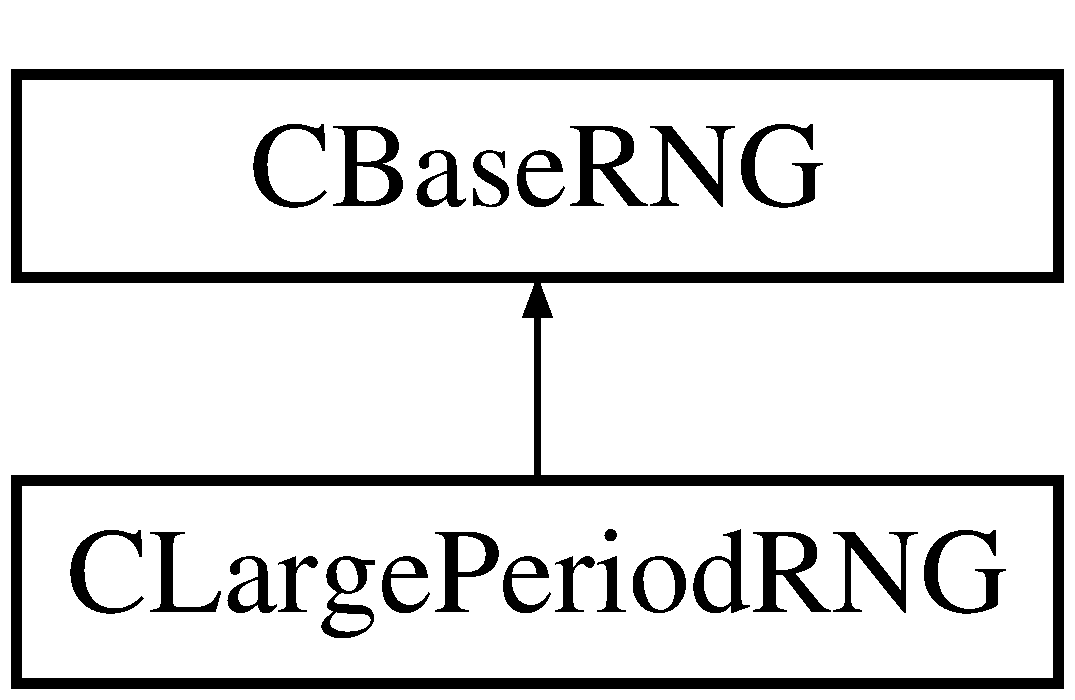
\includegraphics[height=2.000000cm]{class_c_large_period_r_n_g}
\end{center}
\end{figure}
\subsection*{Public Member Functions}
\begin{DoxyCompactItemize}
\item 
\hyperlink{class_c_large_period_r_n_g_af8f1f4ec3712fa7f9534ea6e699913aa}{C\-Large\-Period\-R\-N\-G} ()
\item 
\hyperlink{class_c_large_period_r_n_g_ad70a60b7b4f77d25937360792954c78f}{C\-Large\-Period\-R\-N\-G} (unsigned int s)
\item 
virtual \hyperlink{class_c_large_period_r_n_g_a55def45c2c626bed84c1fd0ede1749f1}{$\sim$\-C\-Large\-Period\-R\-N\-G} ()
\item 
virtual void \hyperlink{class_c_large_period_r_n_g_a59d03465a293ce805a34339f409054d7}{set\-Seed} (unsigned int s)
\begin{DoxyCompactList}\small\item\em Sets seed of the R\-N\-G. \end{DoxyCompactList}\item 
virtual unsigned int \hyperlink{class_c_large_period_r_n_g_aadcf1849be317a7a4dc10500f168d8cd}{rndi} ()
\begin{DoxyCompactList}\small\item\em Returns randomly generated unsigned int. \end{DoxyCompactList}\item 
virtual double \hyperlink{class_c_large_period_r_n_g_a3666cfacb7c24934e7f578ed2b786eb2}{rnd} ()
\begin{DoxyCompactList}\small\item\em Returns randomly generated double between 0 and 1. \end{DoxyCompactList}\end{DoxyCompactItemize}
\subsection*{Private Types}
\begin{DoxyCompactItemize}
\item 
typedef unsigned long long int \hyperlink{class_c_large_period_r_n_g_aaf7ace659133533b97464a9b7538948d}{Ullong}
\end{DoxyCompactItemize}
\subsection*{Private Member Functions}
\begin{DoxyCompactItemize}
\item 
\hyperlink{class_c_large_period_r_n_g_aaf7ace659133533b97464a9b7538948d}{Ullong} \hyperlink{class_c_large_period_r_n_g_a9c27e33ab2331e36123d00d8861aed92}{int64} ()
\end{DoxyCompactItemize}
\subsection*{Private Attributes}
\begin{DoxyCompactItemize}
\item 
\hyperlink{class_c_large_period_r_n_g_aaf7ace659133533b97464a9b7538948d}{Ullong} \hyperlink{class_c_large_period_r_n_g_a6255887a06808f9fe85a65ff86c8fd69}{u}
\item 
\hyperlink{class_c_large_period_r_n_g_aaf7ace659133533b97464a9b7538948d}{Ullong} \hyperlink{class_c_large_period_r_n_g_a544988a3f0eaa81c2eacb9ac8b605c36}{v}
\item 
\hyperlink{class_c_large_period_r_n_g_aaf7ace659133533b97464a9b7538948d}{Ullong} \hyperlink{class_c_large_period_r_n_g_ab26b2dfa899104bb2725f54397df314b}{w}
\begin{DoxyCompactList}\small\item\em Parameters of the large period R\-N\-G. \end{DoxyCompactList}\end{DoxyCompactItemize}


\subsection{Detailed Description}
Class for uniform R\-N\-G with large period = 3.\-138$\ast$10$^\wedge$57. 

\subsection{Member Typedef Documentation}
\hypertarget{class_c_large_period_r_n_g_aaf7ace659133533b97464a9b7538948d}{\index{C\-Large\-Period\-R\-N\-G@{C\-Large\-Period\-R\-N\-G}!Ullong@{Ullong}}
\index{Ullong@{Ullong}!CLargePeriodRNG@{C\-Large\-Period\-R\-N\-G}}
\subsubsection[{Ullong}]{\setlength{\rightskip}{0pt plus 5cm}typedef unsigned long long int {\bf C\-Large\-Period\-R\-N\-G\-::\-Ullong}\hspace{0.3cm}{\ttfamily [private]}}}\label{class_c_large_period_r_n_g_aaf7ace659133533b97464a9b7538948d}


\subsection{Constructor \& Destructor Documentation}
\hypertarget{class_c_large_period_r_n_g_af8f1f4ec3712fa7f9534ea6e699913aa}{\index{C\-Large\-Period\-R\-N\-G@{C\-Large\-Period\-R\-N\-G}!C\-Large\-Period\-R\-N\-G@{C\-Large\-Period\-R\-N\-G}}
\index{C\-Large\-Period\-R\-N\-G@{C\-Large\-Period\-R\-N\-G}!CLargePeriodRNG@{C\-Large\-Period\-R\-N\-G}}
\subsubsection[{C\-Large\-Period\-R\-N\-G}]{\setlength{\rightskip}{0pt plus 5cm}C\-Large\-Period\-R\-N\-G\-::\-C\-Large\-Period\-R\-N\-G (
\begin{DoxyParamCaption}
{}
\end{DoxyParamCaption}
)\hspace{0.3cm}{\ttfamily [inline]}}}\label{class_c_large_period_r_n_g_af8f1f4ec3712fa7f9534ea6e699913aa}
\hypertarget{class_c_large_period_r_n_g_ad70a60b7b4f77d25937360792954c78f}{\index{C\-Large\-Period\-R\-N\-G@{C\-Large\-Period\-R\-N\-G}!C\-Large\-Period\-R\-N\-G@{C\-Large\-Period\-R\-N\-G}}
\index{C\-Large\-Period\-R\-N\-G@{C\-Large\-Period\-R\-N\-G}!CLargePeriodRNG@{C\-Large\-Period\-R\-N\-G}}
\subsubsection[{C\-Large\-Period\-R\-N\-G}]{\setlength{\rightskip}{0pt plus 5cm}C\-Large\-Period\-R\-N\-G\-::\-C\-Large\-Period\-R\-N\-G (
\begin{DoxyParamCaption}
\item[{unsigned int}]{s}
\end{DoxyParamCaption}
)\hspace{0.3cm}{\ttfamily [inline]}}}\label{class_c_large_period_r_n_g_ad70a60b7b4f77d25937360792954c78f}
\hypertarget{class_c_large_period_r_n_g_a55def45c2c626bed84c1fd0ede1749f1}{\index{C\-Large\-Period\-R\-N\-G@{C\-Large\-Period\-R\-N\-G}!$\sim$\-C\-Large\-Period\-R\-N\-G@{$\sim$\-C\-Large\-Period\-R\-N\-G}}
\index{$\sim$\-C\-Large\-Period\-R\-N\-G@{$\sim$\-C\-Large\-Period\-R\-N\-G}!CLargePeriodRNG@{C\-Large\-Period\-R\-N\-G}}
\subsubsection[{$\sim$\-C\-Large\-Period\-R\-N\-G}]{\setlength{\rightskip}{0pt plus 5cm}virtual C\-Large\-Period\-R\-N\-G\-::$\sim$\-C\-Large\-Period\-R\-N\-G (
\begin{DoxyParamCaption}
{}
\end{DoxyParamCaption}
)\hspace{0.3cm}{\ttfamily [inline]}, {\ttfamily [virtual]}}}\label{class_c_large_period_r_n_g_a55def45c2c626bed84c1fd0ede1749f1}


\subsection{Member Function Documentation}
\hypertarget{class_c_large_period_r_n_g_a9c27e33ab2331e36123d00d8861aed92}{\index{C\-Large\-Period\-R\-N\-G@{C\-Large\-Period\-R\-N\-G}!int64@{int64}}
\index{int64@{int64}!CLargePeriodRNG@{C\-Large\-Period\-R\-N\-G}}
\subsubsection[{int64}]{\setlength{\rightskip}{0pt plus 5cm}{\bf Ullong} C\-Large\-Period\-R\-N\-G\-::int64 (
\begin{DoxyParamCaption}
{}
\end{DoxyParamCaption}
)\hspace{0.3cm}{\ttfamily [inline]}, {\ttfamily [private]}}}\label{class_c_large_period_r_n_g_a9c27e33ab2331e36123d00d8861aed92}
\hypertarget{class_c_large_period_r_n_g_a3666cfacb7c24934e7f578ed2b786eb2}{\index{C\-Large\-Period\-R\-N\-G@{C\-Large\-Period\-R\-N\-G}!rnd@{rnd}}
\index{rnd@{rnd}!CLargePeriodRNG@{C\-Large\-Period\-R\-N\-G}}
\subsubsection[{rnd}]{\setlength{\rightskip}{0pt plus 5cm}virtual double C\-Large\-Period\-R\-N\-G\-::rnd (
\begin{DoxyParamCaption}
{}
\end{DoxyParamCaption}
)\hspace{0.3cm}{\ttfamily [inline]}, {\ttfamily [virtual]}}}\label{class_c_large_period_r_n_g_a3666cfacb7c24934e7f578ed2b786eb2}


Returns randomly generated double between 0 and 1. 



Implements \hyperlink{class_c_base_r_n_g_abbd60a5ecdc9502dd646434224ab5d6b}{C\-Base\-R\-N\-G}.

\hypertarget{class_c_large_period_r_n_g_aadcf1849be317a7a4dc10500f168d8cd}{\index{C\-Large\-Period\-R\-N\-G@{C\-Large\-Period\-R\-N\-G}!rndi@{rndi}}
\index{rndi@{rndi}!CLargePeriodRNG@{C\-Large\-Period\-R\-N\-G}}
\subsubsection[{rndi}]{\setlength{\rightskip}{0pt plus 5cm}virtual unsigned int C\-Large\-Period\-R\-N\-G\-::rndi (
\begin{DoxyParamCaption}
{}
\end{DoxyParamCaption}
)\hspace{0.3cm}{\ttfamily [inline]}, {\ttfamily [virtual]}}}\label{class_c_large_period_r_n_g_aadcf1849be317a7a4dc10500f168d8cd}


Returns randomly generated unsigned int. 



Implements \hyperlink{class_c_base_r_n_g_a2db96fbf06a2f11b3613d422043fb7b8}{C\-Base\-R\-N\-G}.

\hypertarget{class_c_large_period_r_n_g_a59d03465a293ce805a34339f409054d7}{\index{C\-Large\-Period\-R\-N\-G@{C\-Large\-Period\-R\-N\-G}!set\-Seed@{set\-Seed}}
\index{set\-Seed@{set\-Seed}!CLargePeriodRNG@{C\-Large\-Period\-R\-N\-G}}
\subsubsection[{set\-Seed}]{\setlength{\rightskip}{0pt plus 5cm}virtual void C\-Large\-Period\-R\-N\-G\-::set\-Seed (
\begin{DoxyParamCaption}
\item[{unsigned int}]{s}
\end{DoxyParamCaption}
)\hspace{0.3cm}{\ttfamily [inline]}, {\ttfamily [virtual]}}}\label{class_c_large_period_r_n_g_a59d03465a293ce805a34339f409054d7}


Sets seed of the R\-N\-G. 


\begin{DoxyParams}{Parameters}
{\em s} & Sets seed of the R\-N\-G. \\
\hline
\end{DoxyParams}


Implements \hyperlink{class_c_base_r_n_g_a56fbf75ca07b73954596ee04820e0b07}{C\-Base\-R\-N\-G}.



\subsection{Member Data Documentation}
\hypertarget{class_c_large_period_r_n_g_a6255887a06808f9fe85a65ff86c8fd69}{\index{C\-Large\-Period\-R\-N\-G@{C\-Large\-Period\-R\-N\-G}!u@{u}}
\index{u@{u}!CLargePeriodRNG@{C\-Large\-Period\-R\-N\-G}}
\subsubsection[{u}]{\setlength{\rightskip}{0pt plus 5cm}{\bf Ullong} C\-Large\-Period\-R\-N\-G\-::u\hspace{0.3cm}{\ttfamily [private]}}}\label{class_c_large_period_r_n_g_a6255887a06808f9fe85a65ff86c8fd69}
\hypertarget{class_c_large_period_r_n_g_a544988a3f0eaa81c2eacb9ac8b605c36}{\index{C\-Large\-Period\-R\-N\-G@{C\-Large\-Period\-R\-N\-G}!v@{v}}
\index{v@{v}!CLargePeriodRNG@{C\-Large\-Period\-R\-N\-G}}
\subsubsection[{v}]{\setlength{\rightskip}{0pt plus 5cm}{\bf Ullong} C\-Large\-Period\-R\-N\-G\-::v\hspace{0.3cm}{\ttfamily [private]}}}\label{class_c_large_period_r_n_g_a544988a3f0eaa81c2eacb9ac8b605c36}
\hypertarget{class_c_large_period_r_n_g_ab26b2dfa899104bb2725f54397df314b}{\index{C\-Large\-Period\-R\-N\-G@{C\-Large\-Period\-R\-N\-G}!w@{w}}
\index{w@{w}!CLargePeriodRNG@{C\-Large\-Period\-R\-N\-G}}
\subsubsection[{w}]{\setlength{\rightskip}{0pt plus 5cm}{\bf Ullong} C\-Large\-Period\-R\-N\-G\-::w\hspace{0.3cm}{\ttfamily [private]}}}\label{class_c_large_period_r_n_g_ab26b2dfa899104bb2725f54397df314b}


Parameters of the large period R\-N\-G. 



The documentation for this class was generated from the following file\-:\begin{DoxyCompactItemize}
\item 
C\-:/\-Development/core/\hyperlink{_random_generators_8h}{Random\-Generators.\-h}\end{DoxyCompactItemize}

\hypertarget{class_go_s_u_m_1_1_c_l_c_voronoi_h_c}{\section{Go\-S\-U\-M\-:\-:C\-L\-C\-Voronoi\-H\-C Class Reference}
\label{class_go_s_u_m_1_1_c_l_c_voronoi_h_c}\index{Go\-S\-U\-M\-::\-C\-L\-C\-Voronoi\-H\-C@{Go\-S\-U\-M\-::\-C\-L\-C\-Voronoi\-H\-C}}
}


{\ttfamily \#include $<$Hypercube.\-h$>$}

Inheritance diagram for Go\-S\-U\-M\-:\-:C\-L\-C\-Voronoi\-H\-C\-:\begin{figure}[H]
\begin{center}
\leavevmode
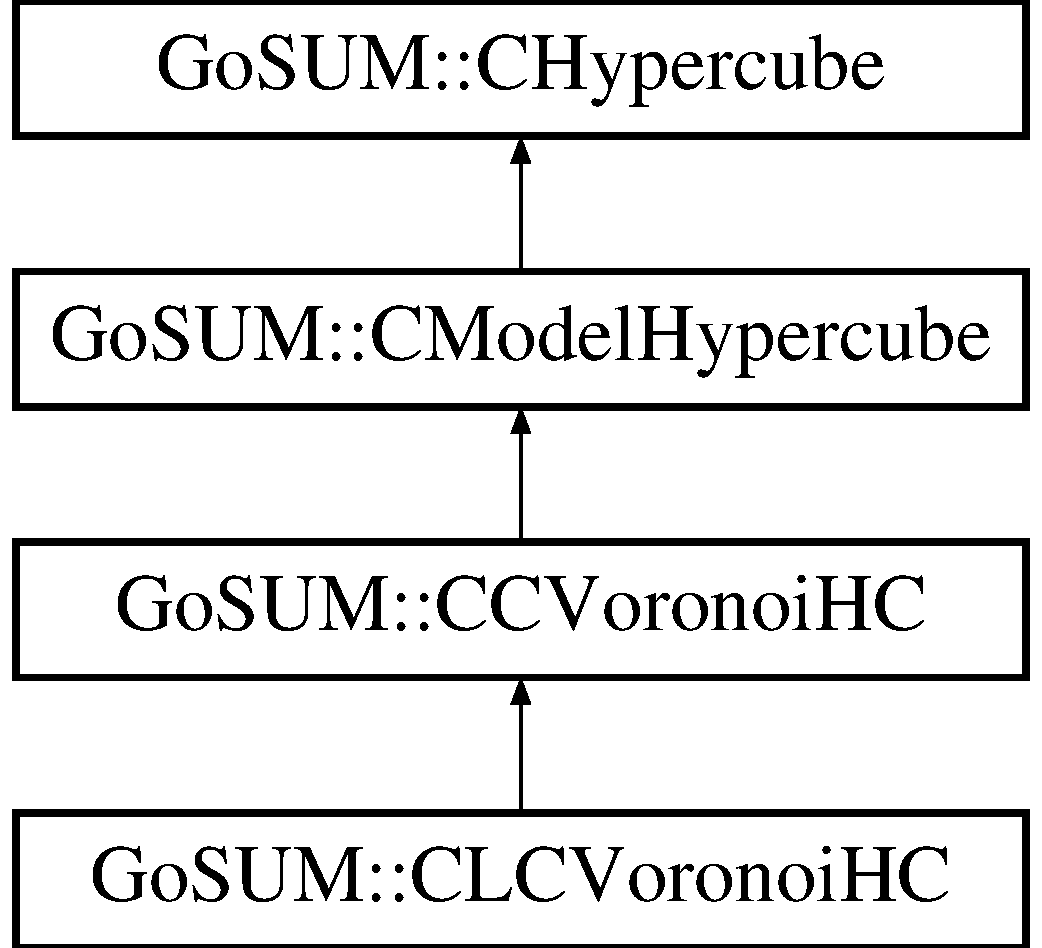
\includegraphics[height=4.000000cm]{class_go_s_u_m_1_1_c_l_c_voronoi_h_c}
\end{center}
\end{figure}
\subsection*{Public Member Functions}
\begin{DoxyCompactItemize}
\item 
\hyperlink{class_go_s_u_m_1_1_c_l_c_voronoi_h_c_a243f56a29444b86e89bd3463582bff46}{C\-L\-C\-Voronoi\-H\-C} (\hyperlink{class_go_s_u_m_1_1_c_input_parameters}{C\-Input\-Parameters} $\ast$\-\_\-p\-I\-P)
\item 
virtual \hyperlink{class_go_s_u_m_1_1_c_l_c_voronoi_h_c_a112c70423f4b76f81f1084e4831ea856}{$\sim$\-C\-L\-C\-Voronoi\-H\-C} ()
\end{DoxyCompactItemize}
\subsection*{Protected Member Functions}
\begin{DoxyCompactItemize}
\item 
{\footnotesize template$<$class Archive $>$ }\\void \hyperlink{class_go_s_u_m_1_1_c_l_c_voronoi_h_c_a98f588c33a8f2e2f4b681b48d63f2109}{serialize} (Archive \&ar, const unsigned int version)
\item 
virtual void \hyperlink{class_go_s_u_m_1_1_c_l_c_voronoi_h_c_a02e90ea8deecafc3b398709f748fa9af}{do\-Generate} (int \-\_\-rssize, int \-\_\-dim, std\-::vector$<$ Array\-Xd $>$ \&\-\_\-samples)
\begin{DoxyCompactList}\small\item\em Core of the generation. \end{DoxyCompactList}\item 
void \hyperlink{class_go_s_u_m_1_1_c_l_c_voronoi_h_c_a5be4f6091986273bdbe421f3b46be9b6}{latinize} (std\-::vector$<$ Array\-Xd $>$ \&\-\_\-samples)
\begin{DoxyCompactList}\small\item\em Latinizes model points \-\_\-samples. \end{DoxyCompactList}\item 
\hyperlink{class_go_s_u_m_1_1_c_l_c_voronoi_h_c_a3f6345253188de13d06c8af6ceab9f16}{C\-L\-C\-Voronoi\-H\-C} ()
\end{DoxyCompactItemize}
\subsection*{Static Protected Member Functions}
\begin{DoxyCompactItemize}
\item 
static bool \hyperlink{class_go_s_u_m_1_1_c_l_c_voronoi_h_c_a5632fe4349c0823b469ed38f005d7717}{compcoo} (Array\-Xd \&a, Array\-Xd \&b)
\end{DoxyCompactItemize}
\subsection*{Static Protected Attributes}
\begin{DoxyCompactItemize}
\item 
static int \hyperlink{class_go_s_u_m_1_1_c_l_c_voronoi_h_c_ad5ec0a5f8490d9de0998266c69ff9ab1}{coo}
\begin{DoxyCompactList}\small\item\em Used in compcoo. \end{DoxyCompactList}\end{DoxyCompactItemize}
\subsection*{Friends}
\begin{DoxyCompactItemize}
\item 
class \hyperlink{class_go_s_u_m_1_1_c_l_c_voronoi_h_c_ac98d07dd8f7b70e16ccb9a01abf56b9c}{boost\-::serialization\-::access}
\begin{DoxyCompactList}\small\item\em Boost serialization. \end{DoxyCompactList}\end{DoxyCompactItemize}
\subsection*{Additional Inherited Members}


\subsection{Constructor \& Destructor Documentation}
\hypertarget{class_go_s_u_m_1_1_c_l_c_voronoi_h_c_a3f6345253188de13d06c8af6ceab9f16}{\index{Go\-S\-U\-M\-::\-C\-L\-C\-Voronoi\-H\-C@{Go\-S\-U\-M\-::\-C\-L\-C\-Voronoi\-H\-C}!C\-L\-C\-Voronoi\-H\-C@{C\-L\-C\-Voronoi\-H\-C}}
\index{C\-L\-C\-Voronoi\-H\-C@{C\-L\-C\-Voronoi\-H\-C}!GoSUM::CLCVoronoiHC@{Go\-S\-U\-M\-::\-C\-L\-C\-Voronoi\-H\-C}}
\subsubsection[{C\-L\-C\-Voronoi\-H\-C}]{\setlength{\rightskip}{0pt plus 5cm}Go\-S\-U\-M\-::\-C\-L\-C\-Voronoi\-H\-C\-::\-C\-L\-C\-Voronoi\-H\-C (
\begin{DoxyParamCaption}
{}
\end{DoxyParamCaption}
)\hspace{0.3cm}{\ttfamily [inline]}, {\ttfamily [protected]}}}\label{class_go_s_u_m_1_1_c_l_c_voronoi_h_c_a3f6345253188de13d06c8af6ceab9f16}
\hypertarget{class_go_s_u_m_1_1_c_l_c_voronoi_h_c_a243f56a29444b86e89bd3463582bff46}{\index{Go\-S\-U\-M\-::\-C\-L\-C\-Voronoi\-H\-C@{Go\-S\-U\-M\-::\-C\-L\-C\-Voronoi\-H\-C}!C\-L\-C\-Voronoi\-H\-C@{C\-L\-C\-Voronoi\-H\-C}}
\index{C\-L\-C\-Voronoi\-H\-C@{C\-L\-C\-Voronoi\-H\-C}!GoSUM::CLCVoronoiHC@{Go\-S\-U\-M\-::\-C\-L\-C\-Voronoi\-H\-C}}
\subsubsection[{C\-L\-C\-Voronoi\-H\-C}]{\setlength{\rightskip}{0pt plus 5cm}Go\-S\-U\-M\-::\-C\-L\-C\-Voronoi\-H\-C\-::\-C\-L\-C\-Voronoi\-H\-C (
\begin{DoxyParamCaption}
\item[{{\bf C\-Input\-Parameters} $\ast$}]{\-\_\-p\-I\-P}
\end{DoxyParamCaption}
)\hspace{0.3cm}{\ttfamily [inline]}}}\label{class_go_s_u_m_1_1_c_l_c_voronoi_h_c_a243f56a29444b86e89bd3463582bff46}
\hypertarget{class_go_s_u_m_1_1_c_l_c_voronoi_h_c_a112c70423f4b76f81f1084e4831ea856}{\index{Go\-S\-U\-M\-::\-C\-L\-C\-Voronoi\-H\-C@{Go\-S\-U\-M\-::\-C\-L\-C\-Voronoi\-H\-C}!$\sim$\-C\-L\-C\-Voronoi\-H\-C@{$\sim$\-C\-L\-C\-Voronoi\-H\-C}}
\index{$\sim$\-C\-L\-C\-Voronoi\-H\-C@{$\sim$\-C\-L\-C\-Voronoi\-H\-C}!GoSUM::CLCVoronoiHC@{Go\-S\-U\-M\-::\-C\-L\-C\-Voronoi\-H\-C}}
\subsubsection[{$\sim$\-C\-L\-C\-Voronoi\-H\-C}]{\setlength{\rightskip}{0pt plus 5cm}virtual Go\-S\-U\-M\-::\-C\-L\-C\-Voronoi\-H\-C\-::$\sim$\-C\-L\-C\-Voronoi\-H\-C (
\begin{DoxyParamCaption}
{}
\end{DoxyParamCaption}
)\hspace{0.3cm}{\ttfamily [inline]}, {\ttfamily [virtual]}}}\label{class_go_s_u_m_1_1_c_l_c_voronoi_h_c_a112c70423f4b76f81f1084e4831ea856}


\subsection{Member Function Documentation}
\hypertarget{class_go_s_u_m_1_1_c_l_c_voronoi_h_c_a5632fe4349c0823b469ed38f005d7717}{\index{Go\-S\-U\-M\-::\-C\-L\-C\-Voronoi\-H\-C@{Go\-S\-U\-M\-::\-C\-L\-C\-Voronoi\-H\-C}!compcoo@{compcoo}}
\index{compcoo@{compcoo}!GoSUM::CLCVoronoiHC@{Go\-S\-U\-M\-::\-C\-L\-C\-Voronoi\-H\-C}}
\subsubsection[{compcoo}]{\setlength{\rightskip}{0pt plus 5cm}static bool Go\-S\-U\-M\-::\-C\-L\-C\-Voronoi\-H\-C\-::compcoo (
\begin{DoxyParamCaption}
\item[{Array\-Xd \&}]{a, }
\item[{Array\-Xd \&}]{b}
\end{DoxyParamCaption}
)\hspace{0.3cm}{\ttfamily [inline]}, {\ttfamily [static]}, {\ttfamily [protected]}}}\label{class_go_s_u_m_1_1_c_l_c_voronoi_h_c_a5632fe4349c0823b469ed38f005d7717}
Compare points by coo cordinate value. \hypertarget{class_go_s_u_m_1_1_c_l_c_voronoi_h_c_a02e90ea8deecafc3b398709f748fa9af}{\index{Go\-S\-U\-M\-::\-C\-L\-C\-Voronoi\-H\-C@{Go\-S\-U\-M\-::\-C\-L\-C\-Voronoi\-H\-C}!do\-Generate@{do\-Generate}}
\index{do\-Generate@{do\-Generate}!GoSUM::CLCVoronoiHC@{Go\-S\-U\-M\-::\-C\-L\-C\-Voronoi\-H\-C}}
\subsubsection[{do\-Generate}]{\setlength{\rightskip}{0pt plus 5cm}void Go\-S\-U\-M\-::\-C\-L\-C\-Voronoi\-H\-C\-::do\-Generate (
\begin{DoxyParamCaption}
\item[{int}]{\-\_\-rssize, }
\item[{int}]{\-\_\-dim, }
\item[{std\-::vector$<$ Array\-Xd $>$ \&}]{\-\_\-samples}
\end{DoxyParamCaption}
)\hspace{0.3cm}{\ttfamily [protected]}, {\ttfamily [virtual]}}}\label{class_go_s_u_m_1_1_c_l_c_voronoi_h_c_a02e90ea8deecafc3b398709f748fa9af}


Core of the generation. 



Reimplemented from \hyperlink{class_go_s_u_m_1_1_c_c_voronoi_h_c_ae3ecc9c8e8c09e42c13b77d0bfa8c020}{Go\-S\-U\-M\-::\-C\-C\-Voronoi\-H\-C}.

\hypertarget{class_go_s_u_m_1_1_c_l_c_voronoi_h_c_a5be4f6091986273bdbe421f3b46be9b6}{\index{Go\-S\-U\-M\-::\-C\-L\-C\-Voronoi\-H\-C@{Go\-S\-U\-M\-::\-C\-L\-C\-Voronoi\-H\-C}!latinize@{latinize}}
\index{latinize@{latinize}!GoSUM::CLCVoronoiHC@{Go\-S\-U\-M\-::\-C\-L\-C\-Voronoi\-H\-C}}
\subsubsection[{latinize}]{\setlength{\rightskip}{0pt plus 5cm}void Go\-S\-U\-M\-::\-C\-L\-C\-Voronoi\-H\-C\-::latinize (
\begin{DoxyParamCaption}
\item[{std\-::vector$<$ Array\-Xd $>$ \&}]{\-\_\-samples}
\end{DoxyParamCaption}
)\hspace{0.3cm}{\ttfamily [protected]}}}\label{class_go_s_u_m_1_1_c_l_c_voronoi_h_c_a5be4f6091986273bdbe421f3b46be9b6}


Latinizes model points \-\_\-samples. 

\hypertarget{class_go_s_u_m_1_1_c_l_c_voronoi_h_c_a98f588c33a8f2e2f4b681b48d63f2109}{\index{Go\-S\-U\-M\-::\-C\-L\-C\-Voronoi\-H\-C@{Go\-S\-U\-M\-::\-C\-L\-C\-Voronoi\-H\-C}!serialize@{serialize}}
\index{serialize@{serialize}!GoSUM::CLCVoronoiHC@{Go\-S\-U\-M\-::\-C\-L\-C\-Voronoi\-H\-C}}
\subsubsection[{serialize}]{\setlength{\rightskip}{0pt plus 5cm}template$<$class Archive $>$ void Go\-S\-U\-M\-::\-C\-L\-C\-Voronoi\-H\-C\-::serialize (
\begin{DoxyParamCaption}
\item[{Archive \&}]{ar, }
\item[{const unsigned int}]{version}
\end{DoxyParamCaption}
)\hspace{0.3cm}{\ttfamily [protected]}}}\label{class_go_s_u_m_1_1_c_l_c_voronoi_h_c_a98f588c33a8f2e2f4b681b48d63f2109}


Reimplemented from \hyperlink{class_go_s_u_m_1_1_c_c_voronoi_h_c_abbeaabd93028069b81be4dfc078e3d02}{Go\-S\-U\-M\-::\-C\-C\-Voronoi\-H\-C}.



\subsection{Friends And Related Function Documentation}
\hypertarget{class_go_s_u_m_1_1_c_l_c_voronoi_h_c_ac98d07dd8f7b70e16ccb9a01abf56b9c}{\index{Go\-S\-U\-M\-::\-C\-L\-C\-Voronoi\-H\-C@{Go\-S\-U\-M\-::\-C\-L\-C\-Voronoi\-H\-C}!boost\-::serialization\-::access@{boost\-::serialization\-::access}}
\index{boost\-::serialization\-::access@{boost\-::serialization\-::access}!GoSUM::CLCVoronoiHC@{Go\-S\-U\-M\-::\-C\-L\-C\-Voronoi\-H\-C}}
\subsubsection[{boost\-::serialization\-::access}]{\setlength{\rightskip}{0pt plus 5cm}friend class boost\-::serialization\-::access\hspace{0.3cm}{\ttfamily [friend]}}}\label{class_go_s_u_m_1_1_c_l_c_voronoi_h_c_ac98d07dd8f7b70e16ccb9a01abf56b9c}


Boost serialization. 



\subsection{Member Data Documentation}
\hypertarget{class_go_s_u_m_1_1_c_l_c_voronoi_h_c_ad5ec0a5f8490d9de0998266c69ff9ab1}{\index{Go\-S\-U\-M\-::\-C\-L\-C\-Voronoi\-H\-C@{Go\-S\-U\-M\-::\-C\-L\-C\-Voronoi\-H\-C}!coo@{coo}}
\index{coo@{coo}!GoSUM::CLCVoronoiHC@{Go\-S\-U\-M\-::\-C\-L\-C\-Voronoi\-H\-C}}
\subsubsection[{coo}]{\setlength{\rightskip}{0pt plus 5cm}int Go\-S\-U\-M\-::\-C\-L\-C\-Voronoi\-H\-C\-::coo\hspace{0.3cm}{\ttfamily [static]}, {\ttfamily [protected]}}}\label{class_go_s_u_m_1_1_c_l_c_voronoi_h_c_ad5ec0a5f8490d9de0998266c69ff9ab1}


Used in compcoo. 



The documentation for this class was generated from the following files\-:\begin{DoxyCompactItemize}
\item 
C\-:/\-Development/core/\hyperlink{_hypercube_8h}{Hypercube.\-h}\item 
C\-:/\-Development/core/\hyperlink{_hypercube_8cpp}{Hypercube.\-cpp}\end{DoxyCompactItemize}

\hypertarget{class_c_m_a_d_s}{\section{C\-M\-A\-D\-S Class Reference}
\label{class_c_m_a_d_s}\index{C\-M\-A\-D\-S@{C\-M\-A\-D\-S}}
}


Class for the mesh addaptive direct serach, i.\-e. interface for N\-O\-M\-A\-D.  




{\ttfamily \#include $<$M\-A\-D\-S\-Optimization.\-h$>$}

\subsection*{Public Member Functions}
\begin{DoxyCompactItemize}
\item 
\hyperlink{class_c_m_a_d_s_a80e31199addf50b5d34bd3aeb7812521}{C\-M\-A\-D\-S} ()
\item 
virtual \hyperlink{class_c_m_a_d_s_af43c613be3091d5ce2523fd21048574a}{$\sim$\-C\-M\-A\-D\-S} ()
\item 
Array\-Xd \hyperlink{class_c_m_a_d_s_a952faa93a4f38ca237dad46d8fec929e}{optimize} (\hyperlink{class_c_optimization_problem}{C\-Optimization\-Problem} $\ast$\-\_\-p\-O\-P, std\-::ostream \&\-\_\-out=std\-::cout)
\begin{DoxyCompactList}\small\item\em Solves the optimizations problem. \end{DoxyCompactList}\item 
int \hyperlink{class_c_m_a_d_s_ad8a920109cf781c8dadca57983f3122f}{evaluation\-Size} () const 
\begin{DoxyCompactList}\small\item\em Returns maximal number of evaluations. \end{DoxyCompactList}\item 
void \hyperlink{class_c_m_a_d_s_ac532678117eb81760fb20a90abaf4f5e}{set\-Evaluation\-Size} (int \-\_\-maxeval)
\begin{DoxyCompactList}\small\item\em Sets maximal number of evaluations. \end{DoxyCompactList}\item 
int \hyperlink{class_c_m_a_d_s_a1cfffca12bdc69f981414c869d80b37c}{initial\-L\-H\-Search} () const 
\begin{DoxyCompactList}\small\item\em Returns initial value for L\-H search. \end{DoxyCompactList}\item 
void \hyperlink{class_c_m_a_d_s_a853551c7d08c15950c881c3add3ced2e}{set\-Initial\-L\-H\-Search} (int \-\_\-lh0)
\begin{DoxyCompactList}\small\item\em Sets initial value for L\-H search. \end{DoxyCompactList}\item 
int \hyperlink{class_c_m_a_d_s_a2e1b3ebc4aabb5ddba0d27b2ef7d69c3}{iteration\-L\-H\-Search} () const 
\begin{DoxyCompactList}\small\item\em Returns iteration value for L\-H search. \end{DoxyCompactList}\item 
void \hyperlink{class_c_m_a_d_s_aa3eb719cc325a85c936ab8a2726823d1}{set\-Iteration\-L\-H\-Search} (int \-\_\-lhi)
\begin{DoxyCompactList}\small\item\em Sets iteration value for L\-H search. \end{DoxyCompactList}\item 
double \hyperlink{class_c_m_a_d_s_a4f7f28c0ef8d53f2fc6c787f2c563ee4}{inital\-Mesh\-Size} () const 
\begin{DoxyCompactList}\small\item\em Returns initial mesh size factor. \end{DoxyCompactList}\item 
void \hyperlink{class_c_m_a_d_s_adaa46855d1352f36c25eaedbeec36e63}{set\-Initial\-Mesh\-Size} (double \-\_\-ims)
\begin{DoxyCompactList}\small\item\em Sets initial mesh size factor. \end{DoxyCompactList}\item 
double \hyperlink{class_c_m_a_d_s_af4c8a983df3b90769230f1e1829af082}{minimal\-Poll\-Size} () const 
\begin{DoxyCompactList}\small\item\em Returns minimal poll size factor. \end{DoxyCompactList}\item 
void \hyperlink{class_c_m_a_d_s_a1580912554dc75226645bc667d5fb1ec}{set\-Minimal\-Poll\-Size} (double \-\_\-mps)
\begin{DoxyCompactList}\small\item\em Sets minimal poll size factor. \end{DoxyCompactList}\item 
int \hyperlink{class_c_m_a_d_s_a1c09eee0705ed297fa20af147e9235bc}{progress\-Steps\-Size} () const 
\begin{DoxyCompactList}\small\item\em Returns progress steps size. \end{DoxyCompactList}\end{DoxyCompactItemize}
\subsection*{Static Public Member Functions}
\begin{DoxyCompactItemize}
\item 
static N\-O\-M\-A\-D\-::\-Point \hyperlink{class_c_m_a_d_s_ad025c8a5bc49648b475ad0f7e744de64}{Array\-Xd2\-N\-O\-M\-A\-D\-Point} (const Array\-Xd \&x)
\begin{DoxyCompactList}\small\item\em Utility\-: converts Array\-Xd to N\-O\-M\-A\-D\-::\-Point. \end{DoxyCompactList}\item 
static Array\-Xd \hyperlink{class_c_m_a_d_s_a0ca8523e34599ee52c7d28027dee33f5}{N\-O\-M\-A\-D\-Point2\-Array\-Xd} (const N\-O\-M\-A\-D\-::\-Point \&p)
\begin{DoxyCompactList}\small\item\em Utility\-: converts N\-O\-M\-A\-D\-::\-Point to Array\-Xd. \end{DoxyCompactList}\end{DoxyCompactItemize}
\subsection*{Protected Member Functions}
\begin{DoxyCompactItemize}
\item 
{\footnotesize template$<$class Archive $>$ }\\void \hyperlink{class_c_m_a_d_s_a1bdfd9d99efd11ad0a0e4051d3897903}{serialize} (Archive \&ar, const unsigned int version)
\end{DoxyCompactItemize}
\subsection*{Protected Attributes}
\begin{DoxyCompactItemize}
\item 
\hyperlink{class_c_optimization_problem}{C\-Optimization\-Problem} $\ast$ \hyperlink{class_c_m_a_d_s_a2df4d9f465992f6130c89fed7880e4e7}{p\-O\-P}
\begin{DoxyCompactList}\small\item\em Points to the optimization problem. \end{DoxyCompactList}\item 
int \hyperlink{class_c_m_a_d_s_ade4448bc470dc7c4c64f890c87f762da}{maxeval}
\begin{DoxyCompactList}\small\item\em Holds maximal number of objective \& constraints evaluations during optimization. \end{DoxyCompactList}\item 
int \hyperlink{class_c_m_a_d_s_a4eaead3a0de0217d182cd70b858c066f}{lh0}
\item 
int \hyperlink{class_c_m_a_d_s_ac6c70518f5b7d42b32f656419406ed7a}{lhi}
\item 
double \hyperlink{class_c_m_a_d_s_a6274e43889cea689ac1bc2d3f2895528}{ims}
\item 
double \hyperlink{class_c_m_a_d_s_a96712dada3b9eb67c28026ac994b5eb1}{mps}
\item 
Array\-Xd \hyperlink{class_c_m_a_d_s_a632620e4e6de702a936648fe4bc8dbe1}{Xbest}
\item 
double \hyperlink{class_c_m_a_d_s_a81f3cabb204f7b152714f65a56f7dac4}{ybest}
\end{DoxyCompactItemize}
\subsection*{Friends}
\begin{DoxyCompactItemize}
\item 
class \hyperlink{class_c_m_a_d_s_ac98d07dd8f7b70e16ccb9a01abf56b9c}{boost\-::serialization\-::access}
\begin{DoxyCompactList}\small\item\em Boost serialization. \end{DoxyCompactList}\end{DoxyCompactItemize}


\subsection{Detailed Description}
Class for the mesh addaptive direct serach, i.\-e. interface for N\-O\-M\-A\-D. 

\subsection{Constructor \& Destructor Documentation}
\hypertarget{class_c_m_a_d_s_a80e31199addf50b5d34bd3aeb7812521}{\index{C\-M\-A\-D\-S@{C\-M\-A\-D\-S}!C\-M\-A\-D\-S@{C\-M\-A\-D\-S}}
\index{C\-M\-A\-D\-S@{C\-M\-A\-D\-S}!CMADS@{C\-M\-A\-D\-S}}
\subsubsection[{C\-M\-A\-D\-S}]{\setlength{\rightskip}{0pt plus 5cm}C\-M\-A\-D\-S\-::\-C\-M\-A\-D\-S (
\begin{DoxyParamCaption}
{}
\end{DoxyParamCaption}
)\hspace{0.3cm}{\ttfamily [inline]}}}\label{class_c_m_a_d_s_a80e31199addf50b5d34bd3aeb7812521}
\hypertarget{class_c_m_a_d_s_af43c613be3091d5ce2523fd21048574a}{\index{C\-M\-A\-D\-S@{C\-M\-A\-D\-S}!$\sim$\-C\-M\-A\-D\-S@{$\sim$\-C\-M\-A\-D\-S}}
\index{$\sim$\-C\-M\-A\-D\-S@{$\sim$\-C\-M\-A\-D\-S}!CMADS@{C\-M\-A\-D\-S}}
\subsubsection[{$\sim$\-C\-M\-A\-D\-S}]{\setlength{\rightskip}{0pt plus 5cm}virtual C\-M\-A\-D\-S\-::$\sim$\-C\-M\-A\-D\-S (
\begin{DoxyParamCaption}
{}
\end{DoxyParamCaption}
)\hspace{0.3cm}{\ttfamily [inline]}, {\ttfamily [virtual]}}}\label{class_c_m_a_d_s_af43c613be3091d5ce2523fd21048574a}


\subsection{Member Function Documentation}
\hypertarget{class_c_m_a_d_s_ad025c8a5bc49648b475ad0f7e744de64}{\index{C\-M\-A\-D\-S@{C\-M\-A\-D\-S}!Array\-Xd2\-N\-O\-M\-A\-D\-Point@{Array\-Xd2\-N\-O\-M\-A\-D\-Point}}
\index{Array\-Xd2\-N\-O\-M\-A\-D\-Point@{Array\-Xd2\-N\-O\-M\-A\-D\-Point}!CMADS@{C\-M\-A\-D\-S}}
\subsubsection[{Array\-Xd2\-N\-O\-M\-A\-D\-Point}]{\setlength{\rightskip}{0pt plus 5cm}N\-O\-M\-A\-D\-::\-Point C\-M\-A\-D\-S\-::\-Array\-Xd2\-N\-O\-M\-A\-D\-Point (
\begin{DoxyParamCaption}
\item[{const Array\-Xd \&}]{x}
\end{DoxyParamCaption}
)\hspace{0.3cm}{\ttfamily [static]}}}\label{class_c_m_a_d_s_ad025c8a5bc49648b475ad0f7e744de64}


Utility\-: converts Array\-Xd to N\-O\-M\-A\-D\-::\-Point. 

\hypertarget{class_c_m_a_d_s_ad8a920109cf781c8dadca57983f3122f}{\index{C\-M\-A\-D\-S@{C\-M\-A\-D\-S}!evaluation\-Size@{evaluation\-Size}}
\index{evaluation\-Size@{evaluation\-Size}!CMADS@{C\-M\-A\-D\-S}}
\subsubsection[{evaluation\-Size}]{\setlength{\rightskip}{0pt plus 5cm}int C\-M\-A\-D\-S\-::evaluation\-Size (
\begin{DoxyParamCaption}
{}
\end{DoxyParamCaption}
) const\hspace{0.3cm}{\ttfamily [inline]}}}\label{class_c_m_a_d_s_ad8a920109cf781c8dadca57983f3122f}


Returns maximal number of evaluations. 

\hypertarget{class_c_m_a_d_s_a4f7f28c0ef8d53f2fc6c787f2c563ee4}{\index{C\-M\-A\-D\-S@{C\-M\-A\-D\-S}!inital\-Mesh\-Size@{inital\-Mesh\-Size}}
\index{inital\-Mesh\-Size@{inital\-Mesh\-Size}!CMADS@{C\-M\-A\-D\-S}}
\subsubsection[{inital\-Mesh\-Size}]{\setlength{\rightskip}{0pt plus 5cm}double C\-M\-A\-D\-S\-::inital\-Mesh\-Size (
\begin{DoxyParamCaption}
{}
\end{DoxyParamCaption}
) const\hspace{0.3cm}{\ttfamily [inline]}}}\label{class_c_m_a_d_s_a4f7f28c0ef8d53f2fc6c787f2c563ee4}


Returns initial mesh size factor. 

\hypertarget{class_c_m_a_d_s_a1cfffca12bdc69f981414c869d80b37c}{\index{C\-M\-A\-D\-S@{C\-M\-A\-D\-S}!initial\-L\-H\-Search@{initial\-L\-H\-Search}}
\index{initial\-L\-H\-Search@{initial\-L\-H\-Search}!CMADS@{C\-M\-A\-D\-S}}
\subsubsection[{initial\-L\-H\-Search}]{\setlength{\rightskip}{0pt plus 5cm}int C\-M\-A\-D\-S\-::initial\-L\-H\-Search (
\begin{DoxyParamCaption}
{}
\end{DoxyParamCaption}
) const\hspace{0.3cm}{\ttfamily [inline]}}}\label{class_c_m_a_d_s_a1cfffca12bdc69f981414c869d80b37c}


Returns initial value for L\-H search. 

\hypertarget{class_c_m_a_d_s_a2e1b3ebc4aabb5ddba0d27b2ef7d69c3}{\index{C\-M\-A\-D\-S@{C\-M\-A\-D\-S}!iteration\-L\-H\-Search@{iteration\-L\-H\-Search}}
\index{iteration\-L\-H\-Search@{iteration\-L\-H\-Search}!CMADS@{C\-M\-A\-D\-S}}
\subsubsection[{iteration\-L\-H\-Search}]{\setlength{\rightskip}{0pt plus 5cm}int C\-M\-A\-D\-S\-::iteration\-L\-H\-Search (
\begin{DoxyParamCaption}
{}
\end{DoxyParamCaption}
) const\hspace{0.3cm}{\ttfamily [inline]}}}\label{class_c_m_a_d_s_a2e1b3ebc4aabb5ddba0d27b2ef7d69c3}


Returns iteration value for L\-H search. 

\hypertarget{class_c_m_a_d_s_af4c8a983df3b90769230f1e1829af082}{\index{C\-M\-A\-D\-S@{C\-M\-A\-D\-S}!minimal\-Poll\-Size@{minimal\-Poll\-Size}}
\index{minimal\-Poll\-Size@{minimal\-Poll\-Size}!CMADS@{C\-M\-A\-D\-S}}
\subsubsection[{minimal\-Poll\-Size}]{\setlength{\rightskip}{0pt plus 5cm}double C\-M\-A\-D\-S\-::minimal\-Poll\-Size (
\begin{DoxyParamCaption}
{}
\end{DoxyParamCaption}
) const\hspace{0.3cm}{\ttfamily [inline]}}}\label{class_c_m_a_d_s_af4c8a983df3b90769230f1e1829af082}


Returns minimal poll size factor. 

\hypertarget{class_c_m_a_d_s_a0ca8523e34599ee52c7d28027dee33f5}{\index{C\-M\-A\-D\-S@{C\-M\-A\-D\-S}!N\-O\-M\-A\-D\-Point2\-Array\-Xd@{N\-O\-M\-A\-D\-Point2\-Array\-Xd}}
\index{N\-O\-M\-A\-D\-Point2\-Array\-Xd@{N\-O\-M\-A\-D\-Point2\-Array\-Xd}!CMADS@{C\-M\-A\-D\-S}}
\subsubsection[{N\-O\-M\-A\-D\-Point2\-Array\-Xd}]{\setlength{\rightskip}{0pt plus 5cm}Array\-Xd C\-M\-A\-D\-S\-::\-N\-O\-M\-A\-D\-Point2\-Array\-Xd (
\begin{DoxyParamCaption}
\item[{const N\-O\-M\-A\-D\-::\-Point \&}]{p}
\end{DoxyParamCaption}
)\hspace{0.3cm}{\ttfamily [static]}}}\label{class_c_m_a_d_s_a0ca8523e34599ee52c7d28027dee33f5}


Utility\-: converts N\-O\-M\-A\-D\-::\-Point to Array\-Xd. 

\hypertarget{class_c_m_a_d_s_a952faa93a4f38ca237dad46d8fec929e}{\index{C\-M\-A\-D\-S@{C\-M\-A\-D\-S}!optimize@{optimize}}
\index{optimize@{optimize}!CMADS@{C\-M\-A\-D\-S}}
\subsubsection[{optimize}]{\setlength{\rightskip}{0pt plus 5cm}Array\-Xd C\-M\-A\-D\-S\-::optimize (
\begin{DoxyParamCaption}
\item[{{\bf C\-Optimization\-Problem} $\ast$}]{\-\_\-p\-O\-P, }
\item[{std\-::ostream \&}]{\-\_\-out = {\ttfamily std\-:\-:cout}}
\end{DoxyParamCaption}
)}}\label{class_c_m_a_d_s_a952faa93a4f38ca237dad46d8fec929e}


Solves the optimizations problem. 

\hypertarget{class_c_m_a_d_s_a1c09eee0705ed297fa20af147e9235bc}{\index{C\-M\-A\-D\-S@{C\-M\-A\-D\-S}!progress\-Steps\-Size@{progress\-Steps\-Size}}
\index{progress\-Steps\-Size@{progress\-Steps\-Size}!CMADS@{C\-M\-A\-D\-S}}
\subsubsection[{progress\-Steps\-Size}]{\setlength{\rightskip}{0pt plus 5cm}int C\-M\-A\-D\-S\-::progress\-Steps\-Size (
\begin{DoxyParamCaption}
{}
\end{DoxyParamCaption}
) const\hspace{0.3cm}{\ttfamily [inline]}}}\label{class_c_m_a_d_s_a1c09eee0705ed297fa20af147e9235bc}


Returns progress steps size. 

\hypertarget{class_c_m_a_d_s_a1bdfd9d99efd11ad0a0e4051d3897903}{\index{C\-M\-A\-D\-S@{C\-M\-A\-D\-S}!serialize@{serialize}}
\index{serialize@{serialize}!CMADS@{C\-M\-A\-D\-S}}
\subsubsection[{serialize}]{\setlength{\rightskip}{0pt plus 5cm}template$<$class Archive $>$ void C\-M\-A\-D\-S\-::serialize (
\begin{DoxyParamCaption}
\item[{Archive \&}]{ar, }
\item[{const unsigned int}]{version}
\end{DoxyParamCaption}
)\hspace{0.3cm}{\ttfamily [protected]}}}\label{class_c_m_a_d_s_a1bdfd9d99efd11ad0a0e4051d3897903}
\hypertarget{class_c_m_a_d_s_ac532678117eb81760fb20a90abaf4f5e}{\index{C\-M\-A\-D\-S@{C\-M\-A\-D\-S}!set\-Evaluation\-Size@{set\-Evaluation\-Size}}
\index{set\-Evaluation\-Size@{set\-Evaluation\-Size}!CMADS@{C\-M\-A\-D\-S}}
\subsubsection[{set\-Evaluation\-Size}]{\setlength{\rightskip}{0pt plus 5cm}void C\-M\-A\-D\-S\-::set\-Evaluation\-Size (
\begin{DoxyParamCaption}
\item[{int}]{\-\_\-maxeval}
\end{DoxyParamCaption}
)\hspace{0.3cm}{\ttfamily [inline]}}}\label{class_c_m_a_d_s_ac532678117eb81760fb20a90abaf4f5e}


Sets maximal number of evaluations. 

\hypertarget{class_c_m_a_d_s_a853551c7d08c15950c881c3add3ced2e}{\index{C\-M\-A\-D\-S@{C\-M\-A\-D\-S}!set\-Initial\-L\-H\-Search@{set\-Initial\-L\-H\-Search}}
\index{set\-Initial\-L\-H\-Search@{set\-Initial\-L\-H\-Search}!CMADS@{C\-M\-A\-D\-S}}
\subsubsection[{set\-Initial\-L\-H\-Search}]{\setlength{\rightskip}{0pt plus 5cm}void C\-M\-A\-D\-S\-::set\-Initial\-L\-H\-Search (
\begin{DoxyParamCaption}
\item[{int}]{\-\_\-lh0}
\end{DoxyParamCaption}
)\hspace{0.3cm}{\ttfamily [inline]}}}\label{class_c_m_a_d_s_a853551c7d08c15950c881c3add3ced2e}


Sets initial value for L\-H search. 

\hypertarget{class_c_m_a_d_s_adaa46855d1352f36c25eaedbeec36e63}{\index{C\-M\-A\-D\-S@{C\-M\-A\-D\-S}!set\-Initial\-Mesh\-Size@{set\-Initial\-Mesh\-Size}}
\index{set\-Initial\-Mesh\-Size@{set\-Initial\-Mesh\-Size}!CMADS@{C\-M\-A\-D\-S}}
\subsubsection[{set\-Initial\-Mesh\-Size}]{\setlength{\rightskip}{0pt plus 5cm}void C\-M\-A\-D\-S\-::set\-Initial\-Mesh\-Size (
\begin{DoxyParamCaption}
\item[{double}]{\-\_\-ims}
\end{DoxyParamCaption}
)\hspace{0.3cm}{\ttfamily [inline]}}}\label{class_c_m_a_d_s_adaa46855d1352f36c25eaedbeec36e63}


Sets initial mesh size factor. 

\hypertarget{class_c_m_a_d_s_aa3eb719cc325a85c936ab8a2726823d1}{\index{C\-M\-A\-D\-S@{C\-M\-A\-D\-S}!set\-Iteration\-L\-H\-Search@{set\-Iteration\-L\-H\-Search}}
\index{set\-Iteration\-L\-H\-Search@{set\-Iteration\-L\-H\-Search}!CMADS@{C\-M\-A\-D\-S}}
\subsubsection[{set\-Iteration\-L\-H\-Search}]{\setlength{\rightskip}{0pt plus 5cm}void C\-M\-A\-D\-S\-::set\-Iteration\-L\-H\-Search (
\begin{DoxyParamCaption}
\item[{int}]{\-\_\-lhi}
\end{DoxyParamCaption}
)\hspace{0.3cm}{\ttfamily [inline]}}}\label{class_c_m_a_d_s_aa3eb719cc325a85c936ab8a2726823d1}


Sets iteration value for L\-H search. 

\hypertarget{class_c_m_a_d_s_a1580912554dc75226645bc667d5fb1ec}{\index{C\-M\-A\-D\-S@{C\-M\-A\-D\-S}!set\-Minimal\-Poll\-Size@{set\-Minimal\-Poll\-Size}}
\index{set\-Minimal\-Poll\-Size@{set\-Minimal\-Poll\-Size}!CMADS@{C\-M\-A\-D\-S}}
\subsubsection[{set\-Minimal\-Poll\-Size}]{\setlength{\rightskip}{0pt plus 5cm}void C\-M\-A\-D\-S\-::set\-Minimal\-Poll\-Size (
\begin{DoxyParamCaption}
\item[{double}]{\-\_\-mps}
\end{DoxyParamCaption}
)\hspace{0.3cm}{\ttfamily [inline]}}}\label{class_c_m_a_d_s_a1580912554dc75226645bc667d5fb1ec}


Sets minimal poll size factor. 



\subsection{Friends And Related Function Documentation}
\hypertarget{class_c_m_a_d_s_ac98d07dd8f7b70e16ccb9a01abf56b9c}{\index{C\-M\-A\-D\-S@{C\-M\-A\-D\-S}!boost\-::serialization\-::access@{boost\-::serialization\-::access}}
\index{boost\-::serialization\-::access@{boost\-::serialization\-::access}!CMADS@{C\-M\-A\-D\-S}}
\subsubsection[{boost\-::serialization\-::access}]{\setlength{\rightskip}{0pt plus 5cm}friend class boost\-::serialization\-::access\hspace{0.3cm}{\ttfamily [friend]}}}\label{class_c_m_a_d_s_ac98d07dd8f7b70e16ccb9a01abf56b9c}


Boost serialization. 



\subsection{Member Data Documentation}
\hypertarget{class_c_m_a_d_s_a6274e43889cea689ac1bc2d3f2895528}{\index{C\-M\-A\-D\-S@{C\-M\-A\-D\-S}!ims@{ims}}
\index{ims@{ims}!CMADS@{C\-M\-A\-D\-S}}
\subsubsection[{ims}]{\setlength{\rightskip}{0pt plus 5cm}double C\-M\-A\-D\-S\-::ims\hspace{0.3cm}{\ttfamily [protected]}}}\label{class_c_m_a_d_s_a6274e43889cea689ac1bc2d3f2895528}
\hypertarget{class_c_m_a_d_s_a4eaead3a0de0217d182cd70b858c066f}{\index{C\-M\-A\-D\-S@{C\-M\-A\-D\-S}!lh0@{lh0}}
\index{lh0@{lh0}!CMADS@{C\-M\-A\-D\-S}}
\subsubsection[{lh0}]{\setlength{\rightskip}{0pt plus 5cm}int C\-M\-A\-D\-S\-::lh0\hspace{0.3cm}{\ttfamily [protected]}}}\label{class_c_m_a_d_s_a4eaead3a0de0217d182cd70b858c066f}
\hypertarget{class_c_m_a_d_s_ac6c70518f5b7d42b32f656419406ed7a}{\index{C\-M\-A\-D\-S@{C\-M\-A\-D\-S}!lhi@{lhi}}
\index{lhi@{lhi}!CMADS@{C\-M\-A\-D\-S}}
\subsubsection[{lhi}]{\setlength{\rightskip}{0pt plus 5cm}int C\-M\-A\-D\-S\-::lhi\hspace{0.3cm}{\ttfamily [protected]}}}\label{class_c_m_a_d_s_ac6c70518f5b7d42b32f656419406ed7a}
\hypertarget{class_c_m_a_d_s_ade4448bc470dc7c4c64f890c87f762da}{\index{C\-M\-A\-D\-S@{C\-M\-A\-D\-S}!maxeval@{maxeval}}
\index{maxeval@{maxeval}!CMADS@{C\-M\-A\-D\-S}}
\subsubsection[{maxeval}]{\setlength{\rightskip}{0pt plus 5cm}int C\-M\-A\-D\-S\-::maxeval\hspace{0.3cm}{\ttfamily [protected]}}}\label{class_c_m_a_d_s_ade4448bc470dc7c4c64f890c87f762da}


Holds maximal number of objective \& constraints evaluations during optimization. 

\hypertarget{class_c_m_a_d_s_a96712dada3b9eb67c28026ac994b5eb1}{\index{C\-M\-A\-D\-S@{C\-M\-A\-D\-S}!mps@{mps}}
\index{mps@{mps}!CMADS@{C\-M\-A\-D\-S}}
\subsubsection[{mps}]{\setlength{\rightskip}{0pt plus 5cm}double C\-M\-A\-D\-S\-::mps\hspace{0.3cm}{\ttfamily [protected]}}}\label{class_c_m_a_d_s_a96712dada3b9eb67c28026ac994b5eb1}
\hypertarget{class_c_m_a_d_s_a2df4d9f465992f6130c89fed7880e4e7}{\index{C\-M\-A\-D\-S@{C\-M\-A\-D\-S}!p\-O\-P@{p\-O\-P}}
\index{p\-O\-P@{p\-O\-P}!CMADS@{C\-M\-A\-D\-S}}
\subsubsection[{p\-O\-P}]{\setlength{\rightskip}{0pt plus 5cm}{\bf C\-Optimization\-Problem}$\ast$ C\-M\-A\-D\-S\-::p\-O\-P\hspace{0.3cm}{\ttfamily [protected]}}}\label{class_c_m_a_d_s_a2df4d9f465992f6130c89fed7880e4e7}


Points to the optimization problem. 

\hypertarget{class_c_m_a_d_s_a632620e4e6de702a936648fe4bc8dbe1}{\index{C\-M\-A\-D\-S@{C\-M\-A\-D\-S}!Xbest@{Xbest}}
\index{Xbest@{Xbest}!CMADS@{C\-M\-A\-D\-S}}
\subsubsection[{Xbest}]{\setlength{\rightskip}{0pt plus 5cm}Array\-Xd C\-M\-A\-D\-S\-::\-Xbest\hspace{0.3cm}{\ttfamily [protected]}}}\label{class_c_m_a_d_s_a632620e4e6de702a936648fe4bc8dbe1}
\hypertarget{class_c_m_a_d_s_a81f3cabb204f7b152714f65a56f7dac4}{\index{C\-M\-A\-D\-S@{C\-M\-A\-D\-S}!ybest@{ybest}}
\index{ybest@{ybest}!CMADS@{C\-M\-A\-D\-S}}
\subsubsection[{ybest}]{\setlength{\rightskip}{0pt plus 5cm}double C\-M\-A\-D\-S\-::ybest\hspace{0.3cm}{\ttfamily [protected]}}}\label{class_c_m_a_d_s_a81f3cabb204f7b152714f65a56f7dac4}


The documentation for this class was generated from the following files\-:\begin{DoxyCompactItemize}
\item 
C\-:/\-Development/core/\hyperlink{_m_a_d_s_optimization_8h}{M\-A\-D\-S\-Optimization.\-h}\item 
C\-:/\-Development/core/\hyperlink{_m_a_d_s_optimization_8cpp}{M\-A\-D\-S\-Optimization.\-cpp}\end{DoxyCompactItemize}

\hypertarget{class_c_m_a_d_s_evaluator}{\section{C\-M\-A\-D\-S\-Evaluator Class Reference}
\label{class_c_m_a_d_s_evaluator}\index{C\-M\-A\-D\-S\-Evaluator@{C\-M\-A\-D\-S\-Evaluator}}
}


Subclass of the N\-O\-M\-A\-D\-::\-Evaluator class.  




{\ttfamily \#include $<$M\-A\-D\-S\-Optimization.\-h$>$}

\subsection*{Public Member Functions}
\begin{DoxyCompactItemize}
\item 
\hyperlink{class_c_m_a_d_s_evaluator_a3ae7243b3f23a630859dcf372178557a}{C\-M\-A\-D\-S\-Evaluator} (const N\-O\-M\-A\-D\-::\-Parameters \&p, \hyperlink{class_c_optimization_problem}{C\-Optimization\-Problem} $\ast$\-\_\-p\-O\-P)
\item 
virtual \hyperlink{class_c_m_a_d_s_evaluator_a75bab21cf6a5fc296e6eb4cfdfb66060}{$\sim$\-C\-M\-A\-D\-S\-Evaluator} ()
\item 
virtual bool \hyperlink{class_c_m_a_d_s_evaluator_a5584e20930e48738e6473a2775202b33}{eval\-\_\-x} (N\-O\-M\-A\-D\-::\-Eval\-\_\-\-Point \&x, const N\-O\-M\-A\-D\-::\-Double \&h\-\_\-max, bool \&count\-\_\-eval) const 
\begin{DoxyCompactList}\small\item\em Overload of the N\-O\-M\-A\-D\-::\-Evaluator evaluation member function. \end{DoxyCompactList}\end{DoxyCompactItemize}
\subsection*{Protected Attributes}
\begin{DoxyCompactItemize}
\item 
\hyperlink{class_c_optimization_problem}{C\-Optimization\-Problem} $\ast$ \hyperlink{class_c_m_a_d_s_evaluator_a49023f451dbaf2b13610074139184e82}{p\-O\-P}
\begin{DoxyCompactList}\small\item\em Points to the optimization problem. \end{DoxyCompactList}\end{DoxyCompactItemize}


\subsection{Detailed Description}
Subclass of the N\-O\-M\-A\-D\-::\-Evaluator class. 

\subsection{Constructor \& Destructor Documentation}
\hypertarget{class_c_m_a_d_s_evaluator_a3ae7243b3f23a630859dcf372178557a}{\index{C\-M\-A\-D\-S\-Evaluator@{C\-M\-A\-D\-S\-Evaluator}!C\-M\-A\-D\-S\-Evaluator@{C\-M\-A\-D\-S\-Evaluator}}
\index{C\-M\-A\-D\-S\-Evaluator@{C\-M\-A\-D\-S\-Evaluator}!CMADSEvaluator@{C\-M\-A\-D\-S\-Evaluator}}
\subsubsection[{C\-M\-A\-D\-S\-Evaluator}]{\setlength{\rightskip}{0pt plus 5cm}C\-M\-A\-D\-S\-Evaluator\-::\-C\-M\-A\-D\-S\-Evaluator (
\begin{DoxyParamCaption}
\item[{const N\-O\-M\-A\-D\-::\-Parameters \&}]{p, }
\item[{{\bf C\-Optimization\-Problem} $\ast$}]{\-\_\-p\-O\-P}
\end{DoxyParamCaption}
)\hspace{0.3cm}{\ttfamily [inline]}}}\label{class_c_m_a_d_s_evaluator_a3ae7243b3f23a630859dcf372178557a}
\hypertarget{class_c_m_a_d_s_evaluator_a75bab21cf6a5fc296e6eb4cfdfb66060}{\index{C\-M\-A\-D\-S\-Evaluator@{C\-M\-A\-D\-S\-Evaluator}!$\sim$\-C\-M\-A\-D\-S\-Evaluator@{$\sim$\-C\-M\-A\-D\-S\-Evaluator}}
\index{$\sim$\-C\-M\-A\-D\-S\-Evaluator@{$\sim$\-C\-M\-A\-D\-S\-Evaluator}!CMADSEvaluator@{C\-M\-A\-D\-S\-Evaluator}}
\subsubsection[{$\sim$\-C\-M\-A\-D\-S\-Evaluator}]{\setlength{\rightskip}{0pt plus 5cm}virtual C\-M\-A\-D\-S\-Evaluator\-::$\sim$\-C\-M\-A\-D\-S\-Evaluator (
\begin{DoxyParamCaption}
{}
\end{DoxyParamCaption}
)\hspace{0.3cm}{\ttfamily [inline]}, {\ttfamily [virtual]}}}\label{class_c_m_a_d_s_evaluator_a75bab21cf6a5fc296e6eb4cfdfb66060}


\subsection{Member Function Documentation}
\hypertarget{class_c_m_a_d_s_evaluator_a5584e20930e48738e6473a2775202b33}{\index{C\-M\-A\-D\-S\-Evaluator@{C\-M\-A\-D\-S\-Evaluator}!eval\-\_\-x@{eval\-\_\-x}}
\index{eval\-\_\-x@{eval\-\_\-x}!CMADSEvaluator@{C\-M\-A\-D\-S\-Evaluator}}
\subsubsection[{eval\-\_\-x}]{\setlength{\rightskip}{0pt plus 5cm}bool C\-M\-A\-D\-S\-Evaluator\-::eval\-\_\-x (
\begin{DoxyParamCaption}
\item[{N\-O\-M\-A\-D\-::\-Eval\-\_\-\-Point \&}]{x, }
\item[{const N\-O\-M\-A\-D\-::\-Double \&}]{h\-\_\-max, }
\item[{bool \&}]{count\-\_\-eval}
\end{DoxyParamCaption}
) const\hspace{0.3cm}{\ttfamily [virtual]}}}\label{class_c_m_a_d_s_evaluator_a5584e20930e48738e6473a2775202b33}


Overload of the N\-O\-M\-A\-D\-::\-Evaluator evaluation member function. 



\subsection{Member Data Documentation}
\hypertarget{class_c_m_a_d_s_evaluator_a49023f451dbaf2b13610074139184e82}{\index{C\-M\-A\-D\-S\-Evaluator@{C\-M\-A\-D\-S\-Evaluator}!p\-O\-P@{p\-O\-P}}
\index{p\-O\-P@{p\-O\-P}!CMADSEvaluator@{C\-M\-A\-D\-S\-Evaluator}}
\subsubsection[{p\-O\-P}]{\setlength{\rightskip}{0pt plus 5cm}{\bf C\-Optimization\-Problem}$\ast$ C\-M\-A\-D\-S\-Evaluator\-::p\-O\-P\hspace{0.3cm}{\ttfamily [protected]}}}\label{class_c_m_a_d_s_evaluator_a49023f451dbaf2b13610074139184e82}


Points to the optimization problem. 



The documentation for this class was generated from the following files\-:\begin{DoxyCompactItemize}
\item 
C\-:/\-Development/core/\hyperlink{_m_a_d_s_optimization_8h}{M\-A\-D\-S\-Optimization.\-h}\item 
C\-:/\-Development/core/\hyperlink{_m_a_d_s_optimization_8cpp}{M\-A\-D\-S\-Optimization.\-cpp}\end{DoxyCompactItemize}

\hypertarget{class_c_m_a_t_l_a_b}{\section{C\-M\-A\-T\-L\-A\-B Class Reference}
\label{class_c_m_a_t_l_a_b}\index{C\-M\-A\-T\-L\-A\-B@{C\-M\-A\-T\-L\-A\-B}}
}


Class interface for Matlab's libmat and libmx dynamic libraries.  




{\ttfamily \#include $<$Matlab\-Library.\-h$>$}

\subsection*{Public Member Functions}
\begin{DoxyCompactItemize}
\item 
\hyperlink{class_c_m_a_t_l_a_b_a51c832deadf847331f9899fe2461e273}{C\-M\-A\-T\-L\-A\-B} ()
\item 
virtual \hyperlink{class_c_m_a_t_l_a_b_a82542c3ead7ba91c54fe71984ca6eff6}{$\sim$\-C\-M\-A\-T\-L\-A\-B} ()
\item 
M\-A\-T\-File $\ast$ \hyperlink{class_c_m_a_t_l_a_b_a44960abdb1f8e8e9b54d383d25b1db74}{mat\-Open} (const string \&filename, const string \&mode)
\begin{DoxyCompactList}\small\item\em Opens mat file using libmat. \end{DoxyCompactList}\item 
bool \hyperlink{class_c_m_a_t_l_a_b_ab81328a4285d9c2ce96a4da6332ad5ac}{mat\-Close} (M\-A\-T\-File $\ast$pmat)
\begin{DoxyCompactList}\small\item\em Closes mat file using libmat. \end{DoxyCompactList}\item 
bool \hyperlink{class_c_m_a_t_l_a_b_a4adc09552978aa43dd03fcdbdf44b08a}{mat\-Put\-Variable} (M\-A\-T\-File $\ast$pmat, const string \&name, const mx\-Array $\ast$pa)
\begin{DoxyCompactList}\small\item\em Puts variable in mat file using libmat. \end{DoxyCompactList}\item 
mx\-Array $\ast$ \hyperlink{class_c_m_a_t_l_a_b_a5e00c5de6806303393696db2153926dd}{mat\-Get\-Variable} (M\-A\-T\-File $\ast$pmat, const string \&name)
\begin{DoxyCompactList}\small\item\em Gets variable from mat file using libmat. \end{DoxyCompactList}\item 
mx\-Array $\ast$ \hyperlink{class_c_m_a_t_l_a_b_ae408d55b19b8f44d766a59958cea73e2}{mx\-Create\-Double\-Matrix} (int N, int M)
\begin{DoxyCompactList}\small\item\em Creats double matrix using libmx. \end{DoxyCompactList}\item 
void \hyperlink{class_c_m_a_t_l_a_b_a86a22fb54ea27d07cf617c544bd47e2c}{mx\-Destroy\-Array} (mx\-Array $\ast$pa)
\begin{DoxyCompactList}\small\item\em Destroys array using libmx. \end{DoxyCompactList}\item 
int \hyperlink{class_c_m_a_t_l_a_b_a9b3c4de338f1db76c505ae86c50f1023}{mx\-Get\-Number\-Of\-Elements} (mx\-Array $\ast$pa)
\begin{DoxyCompactList}\small\item\em Returns number of ements in mx\-Array using libmx. \end{DoxyCompactList}\item 
double $\ast$ \hyperlink{class_c_m_a_t_l_a_b_acdc8c6598199d6d5df97b36cd1864383}{mx\-Get\-Pr} (mx\-Array $\ast$pa)
\begin{DoxyCompactList}\small\item\em Sets data in double matrix using libmx. \end{DoxyCompactList}\item 
Engine $\ast$ \hyperlink{class_c_m_a_t_l_a_b_a15e0b9066c9103355a8223c2922a4a6d}{eng\-Open\-Single\-Use} (const char $\ast$startcmd)
\begin{DoxyCompactList}\small\item\em Opens engine for single use. \end{DoxyCompactList}\item 
Engine $\ast$ \hyperlink{class_c_m_a_t_l_a_b_ac6d7a9542ecc6119dfb7e00024517143}{eng\-Open} (const string \&startcmd)
\begin{DoxyCompactList}\small\item\em Opens engine. \end{DoxyCompactList}\item 
int \hyperlink{class_c_m_a_t_l_a_b_ae68aee94c253c02f5d7318fe1148b889}{eng\-Close} (Engine $\ast$ep)
\begin{DoxyCompactList}\small\item\em Closes engine. \end{DoxyCompactList}\item 
int \hyperlink{class_c_m_a_t_l_a_b_afcedcfb4e40f611ea84da905c40d5906}{eng\-Get\-Visible} (Engine $\ast$ep, bool $\ast$b\-Val)
\begin{DoxyCompactList}\small\item\em Gets if engine is (in)visible. \end{DoxyCompactList}\item 
int \hyperlink{class_c_m_a_t_l_a_b_ab49201f79e5e7ef10e0db6af0a1abdcb}{eng\-Set\-Visible} (Engine $\ast$ep, bool new\-Val)
\begin{DoxyCompactList}\small\item\em Sets engine to (in)visible. \end{DoxyCompactList}\item 
int \hyperlink{class_c_m_a_t_l_a_b_adc555e9306ea2d2c4945661b0af5cd34}{eng\-Eval\-String} (Engine $\ast$ep, const string \&str)
\begin{DoxyCompactList}\small\item\em Gives to engine a string to evaluate. \end{DoxyCompactList}\item 
mx\-Array $\ast$ \hyperlink{class_c_m_a_t_l_a_b_a57bbc476315ce8e01a65167dc971b02f}{eng\-Get\-Variable} (Engine $\ast$ep, const string \&name)
\begin{DoxyCompactList}\small\item\em Gets variable from engine. \end{DoxyCompactList}\item 
int \hyperlink{class_c_m_a_t_l_a_b_aadcd76bf7c7f98e9e08a5e44b93e2e4f}{eng\-Put\-Variable} (Engine $\ast$ep, const string \&var\-\_\-name, const mx\-Array $\ast$ap)
\begin{DoxyCompactList}\small\item\em Puts variable into engine. \end{DoxyCompactList}\item 
int \hyperlink{class_c_m_a_t_l_a_b_a184b784ab8afe19c1003f27a1238b013}{eng\-Output\-Buffer} (Engine $\ast$ep, char $\ast$buffer, int buflen)
\begin{DoxyCompactList}\small\item\em Sets engines output buffer. \end{DoxyCompactList}\item 
void \hyperlink{class_c_m_a_t_l_a_b_ada82733d0bc4be6967e2c7f487abc041}{mat\-Put} (string filename, const Array\-Xd \&X, string Xname)
\begin{DoxyCompactList}\small\item\em Puts 1 array to .mat file. \end{DoxyCompactList}\item 
void \hyperlink{class_c_m_a_t_l_a_b_a22e4a6d97466ecfdc611a9e2970e3fde}{mat\-Get} (string filename, Array\-Xd \&X, string Xname)
\begin{DoxyCompactList}\small\item\em gets 1 array from .mat file. \end{DoxyCompactList}\end{DoxyCompactItemize}
\subsection*{Static Public Member Functions}
\begin{DoxyCompactItemize}
\item 
static void \hyperlink{class_c_m_a_t_l_a_b_a614b714e664e465bd541da7b26a26e59}{Set\-Path} (const std\-::string \&\-\_\-path)
\begin{DoxyCompactList}\small\item\em Sets path to the matlab lib. \end{DoxyCompactList}\item 
static std\-::string \& \hyperlink{class_c_m_a_t_l_a_b_ad72372f5293f1f2cb6bab38229313378}{Path} ()
\begin{DoxyCompactList}\small\item\em Returns path to the matlab lib. \end{DoxyCompactList}\end{DoxyCompactItemize}
\subsection*{Static Public Attributes}
\begin{DoxyCompactItemize}
\item 
static std\-::string \hyperlink{class_c_m_a_t_l_a_b_a3faf4011fa6f7bdd7281e0c5ad10a970}{path} = \char`\"{}C\-:\textbackslash{}\textbackslash{}\-Program Files\textbackslash{}\textbackslash{}\-M\-A\-T\-L\-A\-B\textbackslash{}\textbackslash{}\-R2010b\textbackslash{}\textbackslash{}bin\textbackslash{}\textbackslash{}win64\char`\"{}
\begin{DoxyCompactList}\small\item\em Path to the matlab lib. \end{DoxyCompactList}\end{DoxyCompactItemize}
\subsection*{Private Attributes}
\begin{DoxyCompactItemize}
\item 
Q\-Library \hyperlink{class_c_m_a_t_l_a_b_ad7734632bcf702958838856f46d50f03}{libmat}
\begin{DoxyCompactList}\small\item\em Q\-Library for libmat. \end{DoxyCompactList}\item 
Q\-Library \hyperlink{class_c_m_a_t_l_a_b_ab2aeeea5ac3415555fd88eedaa38b193}{libmx}
\begin{DoxyCompactList}\small\item\em Q\-Library for libmx. \end{DoxyCompactList}\item 
Q\-Library \hyperlink{class_c_m_a_t_l_a_b_af0d1bd46b05565533d973749f5bb9ca3}{libeng}
\begin{DoxyCompactList}\small\item\em Q\-Library for libeng. \end{DoxyCompactList}\item 
\hyperlink{_matlab_library_8h_aca268297c120351425e9c3f63baf7513}{matftype1} \hyperlink{class_c_m_a_t_l_a_b_a6c18b950cb8dbfbba72589e44db1f69e}{p\-Mat\-Open}
\begin{DoxyCompactList}\small\item\em Reference to mat\-Open function from libmat. \end{DoxyCompactList}\item 
\hyperlink{_matlab_library_8h_a13c95ec00742c85c5995ee73f65aa04b}{matftype2} \hyperlink{class_c_m_a_t_l_a_b_a7ec5b3aaa23c3aeac50d7e5e3d0a9dc2}{p\-Mat\-Close}
\begin{DoxyCompactList}\small\item\em Reference to mat\-Close function from libmat. \end{DoxyCompactList}\item 
\hyperlink{_matlab_library_8h_a7160a09ad0d8f7cdf8ddee355882db75}{matftype3} \hyperlink{class_c_m_a_t_l_a_b_ac8ce0e267d00131b74994e825f1bdaa7}{p\-Mat\-Put\-Variable}
\begin{DoxyCompactList}\small\item\em Reference to mat\-Put\-Variable function from libmat. \end{DoxyCompactList}\item 
\hyperlink{_matlab_library_8h_a19aaafe0b8eebabce596da80414ebe6e}{matftype4} \hyperlink{class_c_m_a_t_l_a_b_a67cb7321930f1e73b6b75a461c93316e}{p\-Mat\-Get\-Variable}
\begin{DoxyCompactList}\small\item\em Reference to mat\-Get\-Variable function from libmat. \end{DoxyCompactList}\item 
\hyperlink{_matlab_library_8h_a55b81c948c47f9bfd82db6232884abdd}{mxftype1} \hyperlink{class_c_m_a_t_l_a_b_a39b2341b32007df69682062513aeb208}{p\-Mx\-Create\-Double\-Matrix}
\begin{DoxyCompactList}\small\item\em Reference to mx\-Create\-Double\-Matrix function from libmx. \end{DoxyCompactList}\item 
\hyperlink{_matlab_library_8h_a7022359525610a30ebe4504fff8e3134}{mxftype2} \hyperlink{class_c_m_a_t_l_a_b_ac882abd9bca8e3568632f97f54ac419e}{p\-Mx\-Destroy\-Array}
\begin{DoxyCompactList}\small\item\em Reference to mx\-Destroy\-Array function from libmx. \end{DoxyCompactList}\item 
\hyperlink{_matlab_library_8h_a5c09a212f0d14401cca990067c9f1dbc}{mxftype3} \hyperlink{class_c_m_a_t_l_a_b_ab2647b823dd8a165c7109d0a927d457a}{p\-Mx\-Get\-Pr}
\begin{DoxyCompactList}\small\item\em Reference to mx\-Get\-Pr function from libmx. \end{DoxyCompactList}\item 
\hyperlink{_matlab_library_8h_af4399c0ac6b0e40881ea310c79348f66}{mxftype4} \hyperlink{class_c_m_a_t_l_a_b_a3da6fa87a95db825e0785f4abd761351}{p\-Mx\-Set\-Pr}
\begin{DoxyCompactList}\small\item\em Reference to mx\-Set\-Pr function from libmx. \end{DoxyCompactList}\item 
\hyperlink{_matlab_library_8h_a2b30bc63e1127ad09ffdcb6f160bd48f}{mxftype5} \hyperlink{class_c_m_a_t_l_a_b_ad4e70fa3e8a70bd9ca7bcf6c52b6e9c1}{p\-Mx\-Get\-Number\-Of\-Elements}
\begin{DoxyCompactList}\small\item\em Reference to mx\-Set\-Pr function from libmx. \end{DoxyCompactList}\item 
\hyperlink{_matlab_library_8h_ac4da6e2ee1808b7028f262b520994543}{engftype1} \hyperlink{class_c_m_a_t_l_a_b_a7b65b3c713cf0ace9fe135b94f2ee007}{p\-Eng\-Open\-Single\-Use}
\begin{DoxyCompactList}\small\item\em Reference to eng\-Open\-Single\-Use function from libeng. \end{DoxyCompactList}\item 
\hyperlink{_matlab_library_8h_a8a03b820f78fb36ce5f8f54c883eafbd}{engftype2} \hyperlink{class_c_m_a_t_l_a_b_a22bf0f3a6218ea5ccbff85e603c12455}{p\-Eng\-Open}
\begin{DoxyCompactList}\small\item\em Reference to eng\-Open function from libeng. \end{DoxyCompactList}\item 
\hyperlink{_matlab_library_8h_a3a87349e792acc67028be136d5704897}{engftype3} \hyperlink{class_c_m_a_t_l_a_b_a2afb20fbe0cb6886567c8ef7e024d4bf}{p\-Eng\-Close}
\begin{DoxyCompactList}\small\item\em Reference to eng\-Close function from libeng. \end{DoxyCompactList}\item 
\hyperlink{_matlab_library_8h_af3f2bab0b2bc988ebc51c2eec3eeb121}{engftype4} \hyperlink{class_c_m_a_t_l_a_b_a0e75bb62637fc4c4a4338ad0ca65e193}{p\-Eng\-Get\-Visible}
\begin{DoxyCompactList}\small\item\em Reference to eng\-Get\-Visible function from libeng. \end{DoxyCompactList}\item 
\hyperlink{_matlab_library_8h_ac134537e723ad0d3c52a9a2119ad37cc}{engftype5} \hyperlink{class_c_m_a_t_l_a_b_aacae3122e2253226427bf5ea2d773a7e}{p\-Eng\-Set\-Visible}
\begin{DoxyCompactList}\small\item\em Reference to eng\-Set\-Visible function from libeng. \end{DoxyCompactList}\item 
\hyperlink{_matlab_library_8h_a4746cb1b1e7fec4353d4519d19b8490e}{engftype6} \hyperlink{class_c_m_a_t_l_a_b_aa244761097ed2374d427ad452e693c4e}{p\-Eng\-Eval\-String}
\begin{DoxyCompactList}\small\item\em Reference to eng\-Eval\-String function from libeng. \end{DoxyCompactList}\item 
\hyperlink{_matlab_library_8h_a1764197cbd1c4dbb4a7dc14405d0eaa8}{engftype7} \hyperlink{class_c_m_a_t_l_a_b_a73c962dcd9c9ad01cf0db9fff3346adb}{p\-Eng\-Get\-Variable}
\begin{DoxyCompactList}\small\item\em Reference to eng\-Get\-Variable function from libeng. \end{DoxyCompactList}\item 
\hyperlink{_matlab_library_8h_acc6e68fe4c87fc8b28417a49f7bbf040}{engftype8} \hyperlink{class_c_m_a_t_l_a_b_a2f377cb3dad070f45b0fe6f971f0a8c5}{p\-Eng\-Put\-Variable}
\begin{DoxyCompactList}\small\item\em Reference to eng\-Put\-Variable function from libeng. \end{DoxyCompactList}\item 
\hyperlink{_matlab_library_8h_a49ce13d36241af0257a6b66c29a65131}{engftype9} \hyperlink{class_c_m_a_t_l_a_b_a41eefdf98cf7dca3f766c3378b022746}{p\-Eng\-Output\-Buffer}
\begin{DoxyCompactList}\small\item\em Reference to eng\-Output\-Buffer function from libeng. \end{DoxyCompactList}\end{DoxyCompactItemize}


\subsection{Detailed Description}
Class interface for Matlab's libmat and libmx dynamic libraries. 

\subsection{Constructor \& Destructor Documentation}
\hypertarget{class_c_m_a_t_l_a_b_a51c832deadf847331f9899fe2461e273}{\index{C\-M\-A\-T\-L\-A\-B@{C\-M\-A\-T\-L\-A\-B}!C\-M\-A\-T\-L\-A\-B@{C\-M\-A\-T\-L\-A\-B}}
\index{C\-M\-A\-T\-L\-A\-B@{C\-M\-A\-T\-L\-A\-B}!CMATLAB@{C\-M\-A\-T\-L\-A\-B}}
\subsubsection[{C\-M\-A\-T\-L\-A\-B}]{\setlength{\rightskip}{0pt plus 5cm}C\-M\-A\-T\-L\-A\-B\-::\-C\-M\-A\-T\-L\-A\-B (
\begin{DoxyParamCaption}
{}
\end{DoxyParamCaption}
)}}\label{class_c_m_a_t_l_a_b_a51c832deadf847331f9899fe2461e273}
\hypertarget{class_c_m_a_t_l_a_b_a82542c3ead7ba91c54fe71984ca6eff6}{\index{C\-M\-A\-T\-L\-A\-B@{C\-M\-A\-T\-L\-A\-B}!$\sim$\-C\-M\-A\-T\-L\-A\-B@{$\sim$\-C\-M\-A\-T\-L\-A\-B}}
\index{$\sim$\-C\-M\-A\-T\-L\-A\-B@{$\sim$\-C\-M\-A\-T\-L\-A\-B}!CMATLAB@{C\-M\-A\-T\-L\-A\-B}}
\subsubsection[{$\sim$\-C\-M\-A\-T\-L\-A\-B}]{\setlength{\rightskip}{0pt plus 5cm}virtual C\-M\-A\-T\-L\-A\-B\-::$\sim$\-C\-M\-A\-T\-L\-A\-B (
\begin{DoxyParamCaption}
{}
\end{DoxyParamCaption}
)\hspace{0.3cm}{\ttfamily [inline]}, {\ttfamily [virtual]}}}\label{class_c_m_a_t_l_a_b_a82542c3ead7ba91c54fe71984ca6eff6}


\subsection{Member Function Documentation}
\hypertarget{class_c_m_a_t_l_a_b_ae68aee94c253c02f5d7318fe1148b889}{\index{C\-M\-A\-T\-L\-A\-B@{C\-M\-A\-T\-L\-A\-B}!eng\-Close@{eng\-Close}}
\index{eng\-Close@{eng\-Close}!CMATLAB@{C\-M\-A\-T\-L\-A\-B}}
\subsubsection[{eng\-Close}]{\setlength{\rightskip}{0pt plus 5cm}int C\-M\-A\-T\-L\-A\-B\-::eng\-Close (
\begin{DoxyParamCaption}
\item[{Engine $\ast$}]{ep}
\end{DoxyParamCaption}
)\hspace{0.3cm}{\ttfamily [inline]}}}\label{class_c_m_a_t_l_a_b_ae68aee94c253c02f5d7318fe1148b889}


Closes engine. 

\hypertarget{class_c_m_a_t_l_a_b_adc555e9306ea2d2c4945661b0af5cd34}{\index{C\-M\-A\-T\-L\-A\-B@{C\-M\-A\-T\-L\-A\-B}!eng\-Eval\-String@{eng\-Eval\-String}}
\index{eng\-Eval\-String@{eng\-Eval\-String}!CMATLAB@{C\-M\-A\-T\-L\-A\-B}}
\subsubsection[{eng\-Eval\-String}]{\setlength{\rightskip}{0pt plus 5cm}int C\-M\-A\-T\-L\-A\-B\-::eng\-Eval\-String (
\begin{DoxyParamCaption}
\item[{Engine $\ast$}]{ep, }
\item[{const string \&}]{str}
\end{DoxyParamCaption}
)\hspace{0.3cm}{\ttfamily [inline]}}}\label{class_c_m_a_t_l_a_b_adc555e9306ea2d2c4945661b0af5cd34}


Gives to engine a string to evaluate. 

\hypertarget{class_c_m_a_t_l_a_b_a57bbc476315ce8e01a65167dc971b02f}{\index{C\-M\-A\-T\-L\-A\-B@{C\-M\-A\-T\-L\-A\-B}!eng\-Get\-Variable@{eng\-Get\-Variable}}
\index{eng\-Get\-Variable@{eng\-Get\-Variable}!CMATLAB@{C\-M\-A\-T\-L\-A\-B}}
\subsubsection[{eng\-Get\-Variable}]{\setlength{\rightskip}{0pt plus 5cm}mx\-Array$\ast$ C\-M\-A\-T\-L\-A\-B\-::eng\-Get\-Variable (
\begin{DoxyParamCaption}
\item[{Engine $\ast$}]{ep, }
\item[{const string \&}]{name}
\end{DoxyParamCaption}
)\hspace{0.3cm}{\ttfamily [inline]}}}\label{class_c_m_a_t_l_a_b_a57bbc476315ce8e01a65167dc971b02f}


Gets variable from engine. 

\hypertarget{class_c_m_a_t_l_a_b_afcedcfb4e40f611ea84da905c40d5906}{\index{C\-M\-A\-T\-L\-A\-B@{C\-M\-A\-T\-L\-A\-B}!eng\-Get\-Visible@{eng\-Get\-Visible}}
\index{eng\-Get\-Visible@{eng\-Get\-Visible}!CMATLAB@{C\-M\-A\-T\-L\-A\-B}}
\subsubsection[{eng\-Get\-Visible}]{\setlength{\rightskip}{0pt plus 5cm}int C\-M\-A\-T\-L\-A\-B\-::eng\-Get\-Visible (
\begin{DoxyParamCaption}
\item[{Engine $\ast$}]{ep, }
\item[{bool $\ast$}]{b\-Val}
\end{DoxyParamCaption}
)\hspace{0.3cm}{\ttfamily [inline]}}}\label{class_c_m_a_t_l_a_b_afcedcfb4e40f611ea84da905c40d5906}


Gets if engine is (in)visible. 

\hypertarget{class_c_m_a_t_l_a_b_ac6d7a9542ecc6119dfb7e00024517143}{\index{C\-M\-A\-T\-L\-A\-B@{C\-M\-A\-T\-L\-A\-B}!eng\-Open@{eng\-Open}}
\index{eng\-Open@{eng\-Open}!CMATLAB@{C\-M\-A\-T\-L\-A\-B}}
\subsubsection[{eng\-Open}]{\setlength{\rightskip}{0pt plus 5cm}Engine$\ast$ C\-M\-A\-T\-L\-A\-B\-::eng\-Open (
\begin{DoxyParamCaption}
\item[{const string \&}]{startcmd}
\end{DoxyParamCaption}
)\hspace{0.3cm}{\ttfamily [inline]}}}\label{class_c_m_a_t_l_a_b_ac6d7a9542ecc6119dfb7e00024517143}


Opens engine. 

\hypertarget{class_c_m_a_t_l_a_b_a15e0b9066c9103355a8223c2922a4a6d}{\index{C\-M\-A\-T\-L\-A\-B@{C\-M\-A\-T\-L\-A\-B}!eng\-Open\-Single\-Use@{eng\-Open\-Single\-Use}}
\index{eng\-Open\-Single\-Use@{eng\-Open\-Single\-Use}!CMATLAB@{C\-M\-A\-T\-L\-A\-B}}
\subsubsection[{eng\-Open\-Single\-Use}]{\setlength{\rightskip}{0pt plus 5cm}Engine$\ast$ C\-M\-A\-T\-L\-A\-B\-::eng\-Open\-Single\-Use (
\begin{DoxyParamCaption}
\item[{const char $\ast$}]{startcmd}
\end{DoxyParamCaption}
)\hspace{0.3cm}{\ttfamily [inline]}}}\label{class_c_m_a_t_l_a_b_a15e0b9066c9103355a8223c2922a4a6d}


Opens engine for single use. 

\hypertarget{class_c_m_a_t_l_a_b_a184b784ab8afe19c1003f27a1238b013}{\index{C\-M\-A\-T\-L\-A\-B@{C\-M\-A\-T\-L\-A\-B}!eng\-Output\-Buffer@{eng\-Output\-Buffer}}
\index{eng\-Output\-Buffer@{eng\-Output\-Buffer}!CMATLAB@{C\-M\-A\-T\-L\-A\-B}}
\subsubsection[{eng\-Output\-Buffer}]{\setlength{\rightskip}{0pt plus 5cm}int C\-M\-A\-T\-L\-A\-B\-::eng\-Output\-Buffer (
\begin{DoxyParamCaption}
\item[{Engine $\ast$}]{ep, }
\item[{char $\ast$}]{buffer, }
\item[{int}]{buflen}
\end{DoxyParamCaption}
)\hspace{0.3cm}{\ttfamily [inline]}}}\label{class_c_m_a_t_l_a_b_a184b784ab8afe19c1003f27a1238b013}


Sets engines output buffer. 

\hypertarget{class_c_m_a_t_l_a_b_aadcd76bf7c7f98e9e08a5e44b93e2e4f}{\index{C\-M\-A\-T\-L\-A\-B@{C\-M\-A\-T\-L\-A\-B}!eng\-Put\-Variable@{eng\-Put\-Variable}}
\index{eng\-Put\-Variable@{eng\-Put\-Variable}!CMATLAB@{C\-M\-A\-T\-L\-A\-B}}
\subsubsection[{eng\-Put\-Variable}]{\setlength{\rightskip}{0pt plus 5cm}int C\-M\-A\-T\-L\-A\-B\-::eng\-Put\-Variable (
\begin{DoxyParamCaption}
\item[{Engine $\ast$}]{ep, }
\item[{const string \&}]{var\-\_\-name, }
\item[{const mx\-Array $\ast$}]{ap}
\end{DoxyParamCaption}
)\hspace{0.3cm}{\ttfamily [inline]}}}\label{class_c_m_a_t_l_a_b_aadcd76bf7c7f98e9e08a5e44b93e2e4f}


Puts variable into engine. 

\hypertarget{class_c_m_a_t_l_a_b_ab49201f79e5e7ef10e0db6af0a1abdcb}{\index{C\-M\-A\-T\-L\-A\-B@{C\-M\-A\-T\-L\-A\-B}!eng\-Set\-Visible@{eng\-Set\-Visible}}
\index{eng\-Set\-Visible@{eng\-Set\-Visible}!CMATLAB@{C\-M\-A\-T\-L\-A\-B}}
\subsubsection[{eng\-Set\-Visible}]{\setlength{\rightskip}{0pt plus 5cm}int C\-M\-A\-T\-L\-A\-B\-::eng\-Set\-Visible (
\begin{DoxyParamCaption}
\item[{Engine $\ast$}]{ep, }
\item[{bool}]{new\-Val}
\end{DoxyParamCaption}
)\hspace{0.3cm}{\ttfamily [inline]}}}\label{class_c_m_a_t_l_a_b_ab49201f79e5e7ef10e0db6af0a1abdcb}


Sets engine to (in)visible. 

\hypertarget{class_c_m_a_t_l_a_b_ab81328a4285d9c2ce96a4da6332ad5ac}{\index{C\-M\-A\-T\-L\-A\-B@{C\-M\-A\-T\-L\-A\-B}!mat\-Close@{mat\-Close}}
\index{mat\-Close@{mat\-Close}!CMATLAB@{C\-M\-A\-T\-L\-A\-B}}
\subsubsection[{mat\-Close}]{\setlength{\rightskip}{0pt plus 5cm}bool C\-M\-A\-T\-L\-A\-B\-::mat\-Close (
\begin{DoxyParamCaption}
\item[{M\-A\-T\-File $\ast$}]{pmat}
\end{DoxyParamCaption}
)\hspace{0.3cm}{\ttfamily [inline]}}}\label{class_c_m_a_t_l_a_b_ab81328a4285d9c2ce96a4da6332ad5ac}


Closes mat file using libmat. 

\hypertarget{class_c_m_a_t_l_a_b_a22e4a6d97466ecfdc611a9e2970e3fde}{\index{C\-M\-A\-T\-L\-A\-B@{C\-M\-A\-T\-L\-A\-B}!mat\-Get@{mat\-Get}}
\index{mat\-Get@{mat\-Get}!CMATLAB@{C\-M\-A\-T\-L\-A\-B}}
\subsubsection[{mat\-Get}]{\setlength{\rightskip}{0pt plus 5cm}void C\-M\-A\-T\-L\-A\-B\-::mat\-Get (
\begin{DoxyParamCaption}
\item[{string}]{filename, }
\item[{Array\-Xd \&}]{X, }
\item[{string}]{Xname}
\end{DoxyParamCaption}
)}}\label{class_c_m_a_t_l_a_b_a22e4a6d97466ecfdc611a9e2970e3fde}


gets 1 array from .mat file. 

\hypertarget{class_c_m_a_t_l_a_b_a5e00c5de6806303393696db2153926dd}{\index{C\-M\-A\-T\-L\-A\-B@{C\-M\-A\-T\-L\-A\-B}!mat\-Get\-Variable@{mat\-Get\-Variable}}
\index{mat\-Get\-Variable@{mat\-Get\-Variable}!CMATLAB@{C\-M\-A\-T\-L\-A\-B}}
\subsubsection[{mat\-Get\-Variable}]{\setlength{\rightskip}{0pt plus 5cm}mx\-Array$\ast$ C\-M\-A\-T\-L\-A\-B\-::mat\-Get\-Variable (
\begin{DoxyParamCaption}
\item[{M\-A\-T\-File $\ast$}]{pmat, }
\item[{const string \&}]{name}
\end{DoxyParamCaption}
)\hspace{0.3cm}{\ttfamily [inline]}}}\label{class_c_m_a_t_l_a_b_a5e00c5de6806303393696db2153926dd}


Gets variable from mat file using libmat. 

\hypertarget{class_c_m_a_t_l_a_b_a44960abdb1f8e8e9b54d383d25b1db74}{\index{C\-M\-A\-T\-L\-A\-B@{C\-M\-A\-T\-L\-A\-B}!mat\-Open@{mat\-Open}}
\index{mat\-Open@{mat\-Open}!CMATLAB@{C\-M\-A\-T\-L\-A\-B}}
\subsubsection[{mat\-Open}]{\setlength{\rightskip}{0pt plus 5cm}M\-A\-T\-File$\ast$ C\-M\-A\-T\-L\-A\-B\-::mat\-Open (
\begin{DoxyParamCaption}
\item[{const string \&}]{filename, }
\item[{const string \&}]{mode}
\end{DoxyParamCaption}
)\hspace{0.3cm}{\ttfamily [inline]}}}\label{class_c_m_a_t_l_a_b_a44960abdb1f8e8e9b54d383d25b1db74}


Opens mat file using libmat. 

\hypertarget{class_c_m_a_t_l_a_b_ada82733d0bc4be6967e2c7f487abc041}{\index{C\-M\-A\-T\-L\-A\-B@{C\-M\-A\-T\-L\-A\-B}!mat\-Put@{mat\-Put}}
\index{mat\-Put@{mat\-Put}!CMATLAB@{C\-M\-A\-T\-L\-A\-B}}
\subsubsection[{mat\-Put}]{\setlength{\rightskip}{0pt plus 5cm}void C\-M\-A\-T\-L\-A\-B\-::mat\-Put (
\begin{DoxyParamCaption}
\item[{string}]{filename, }
\item[{const Array\-Xd \&}]{X, }
\item[{string}]{Xname}
\end{DoxyParamCaption}
)}}\label{class_c_m_a_t_l_a_b_ada82733d0bc4be6967e2c7f487abc041}


Puts 1 array to .mat file. 

\hypertarget{class_c_m_a_t_l_a_b_a4adc09552978aa43dd03fcdbdf44b08a}{\index{C\-M\-A\-T\-L\-A\-B@{C\-M\-A\-T\-L\-A\-B}!mat\-Put\-Variable@{mat\-Put\-Variable}}
\index{mat\-Put\-Variable@{mat\-Put\-Variable}!CMATLAB@{C\-M\-A\-T\-L\-A\-B}}
\subsubsection[{mat\-Put\-Variable}]{\setlength{\rightskip}{0pt plus 5cm}bool C\-M\-A\-T\-L\-A\-B\-::mat\-Put\-Variable (
\begin{DoxyParamCaption}
\item[{M\-A\-T\-File $\ast$}]{pmat, }
\item[{const string \&}]{name, }
\item[{const mx\-Array $\ast$}]{pa}
\end{DoxyParamCaption}
)\hspace{0.3cm}{\ttfamily [inline]}}}\label{class_c_m_a_t_l_a_b_a4adc09552978aa43dd03fcdbdf44b08a}


Puts variable in mat file using libmat. 

\hypertarget{class_c_m_a_t_l_a_b_ae408d55b19b8f44d766a59958cea73e2}{\index{C\-M\-A\-T\-L\-A\-B@{C\-M\-A\-T\-L\-A\-B}!mx\-Create\-Double\-Matrix@{mx\-Create\-Double\-Matrix}}
\index{mx\-Create\-Double\-Matrix@{mx\-Create\-Double\-Matrix}!CMATLAB@{C\-M\-A\-T\-L\-A\-B}}
\subsubsection[{mx\-Create\-Double\-Matrix}]{\setlength{\rightskip}{0pt plus 5cm}mx\-Array$\ast$ C\-M\-A\-T\-L\-A\-B\-::mx\-Create\-Double\-Matrix (
\begin{DoxyParamCaption}
\item[{int}]{N, }
\item[{int}]{M}
\end{DoxyParamCaption}
)\hspace{0.3cm}{\ttfamily [inline]}}}\label{class_c_m_a_t_l_a_b_ae408d55b19b8f44d766a59958cea73e2}


Creats double matrix using libmx. 

\hypertarget{class_c_m_a_t_l_a_b_a86a22fb54ea27d07cf617c544bd47e2c}{\index{C\-M\-A\-T\-L\-A\-B@{C\-M\-A\-T\-L\-A\-B}!mx\-Destroy\-Array@{mx\-Destroy\-Array}}
\index{mx\-Destroy\-Array@{mx\-Destroy\-Array}!CMATLAB@{C\-M\-A\-T\-L\-A\-B}}
\subsubsection[{mx\-Destroy\-Array}]{\setlength{\rightskip}{0pt plus 5cm}void C\-M\-A\-T\-L\-A\-B\-::mx\-Destroy\-Array (
\begin{DoxyParamCaption}
\item[{mx\-Array $\ast$}]{pa}
\end{DoxyParamCaption}
)\hspace{0.3cm}{\ttfamily [inline]}}}\label{class_c_m_a_t_l_a_b_a86a22fb54ea27d07cf617c544bd47e2c}


Destroys array using libmx. 

\hypertarget{class_c_m_a_t_l_a_b_a9b3c4de338f1db76c505ae86c50f1023}{\index{C\-M\-A\-T\-L\-A\-B@{C\-M\-A\-T\-L\-A\-B}!mx\-Get\-Number\-Of\-Elements@{mx\-Get\-Number\-Of\-Elements}}
\index{mx\-Get\-Number\-Of\-Elements@{mx\-Get\-Number\-Of\-Elements}!CMATLAB@{C\-M\-A\-T\-L\-A\-B}}
\subsubsection[{mx\-Get\-Number\-Of\-Elements}]{\setlength{\rightskip}{0pt plus 5cm}int C\-M\-A\-T\-L\-A\-B\-::mx\-Get\-Number\-Of\-Elements (
\begin{DoxyParamCaption}
\item[{mx\-Array $\ast$}]{pa}
\end{DoxyParamCaption}
)\hspace{0.3cm}{\ttfamily [inline]}}}\label{class_c_m_a_t_l_a_b_a9b3c4de338f1db76c505ae86c50f1023}


Returns number of ements in mx\-Array using libmx. 

\hypertarget{class_c_m_a_t_l_a_b_acdc8c6598199d6d5df97b36cd1864383}{\index{C\-M\-A\-T\-L\-A\-B@{C\-M\-A\-T\-L\-A\-B}!mx\-Get\-Pr@{mx\-Get\-Pr}}
\index{mx\-Get\-Pr@{mx\-Get\-Pr}!CMATLAB@{C\-M\-A\-T\-L\-A\-B}}
\subsubsection[{mx\-Get\-Pr}]{\setlength{\rightskip}{0pt plus 5cm}double$\ast$ C\-M\-A\-T\-L\-A\-B\-::mx\-Get\-Pr (
\begin{DoxyParamCaption}
\item[{mx\-Array $\ast$}]{pa}
\end{DoxyParamCaption}
)\hspace{0.3cm}{\ttfamily [inline]}}}\label{class_c_m_a_t_l_a_b_acdc8c6598199d6d5df97b36cd1864383}


Sets data in double matrix using libmx. 

\hypertarget{class_c_m_a_t_l_a_b_ad72372f5293f1f2cb6bab38229313378}{\index{C\-M\-A\-T\-L\-A\-B@{C\-M\-A\-T\-L\-A\-B}!Path@{Path}}
\index{Path@{Path}!CMATLAB@{C\-M\-A\-T\-L\-A\-B}}
\subsubsection[{Path}]{\setlength{\rightskip}{0pt plus 5cm}std\-::string \& C\-M\-A\-T\-L\-A\-B\-::\-Path (
\begin{DoxyParamCaption}
{}
\end{DoxyParamCaption}
)\hspace{0.3cm}{\ttfamily [static]}}}\label{class_c_m_a_t_l_a_b_ad72372f5293f1f2cb6bab38229313378}


Returns path to the matlab lib. 

\hypertarget{class_c_m_a_t_l_a_b_a614b714e664e465bd541da7b26a26e59}{\index{C\-M\-A\-T\-L\-A\-B@{C\-M\-A\-T\-L\-A\-B}!Set\-Path@{Set\-Path}}
\index{Set\-Path@{Set\-Path}!CMATLAB@{C\-M\-A\-T\-L\-A\-B}}
\subsubsection[{Set\-Path}]{\setlength{\rightskip}{0pt plus 5cm}void C\-M\-A\-T\-L\-A\-B\-::\-Set\-Path (
\begin{DoxyParamCaption}
\item[{const std\-::string \&}]{\-\_\-path}
\end{DoxyParamCaption}
)\hspace{0.3cm}{\ttfamily [static]}}}\label{class_c_m_a_t_l_a_b_a614b714e664e465bd541da7b26a26e59}


Sets path to the matlab lib. 



\subsection{Member Data Documentation}
\hypertarget{class_c_m_a_t_l_a_b_af0d1bd46b05565533d973749f5bb9ca3}{\index{C\-M\-A\-T\-L\-A\-B@{C\-M\-A\-T\-L\-A\-B}!libeng@{libeng}}
\index{libeng@{libeng}!CMATLAB@{C\-M\-A\-T\-L\-A\-B}}
\subsubsection[{libeng}]{\setlength{\rightskip}{0pt plus 5cm}Q\-Library C\-M\-A\-T\-L\-A\-B\-::libeng\hspace{0.3cm}{\ttfamily [private]}}}\label{class_c_m_a_t_l_a_b_af0d1bd46b05565533d973749f5bb9ca3}


Q\-Library for libeng. 

\hypertarget{class_c_m_a_t_l_a_b_ad7734632bcf702958838856f46d50f03}{\index{C\-M\-A\-T\-L\-A\-B@{C\-M\-A\-T\-L\-A\-B}!libmat@{libmat}}
\index{libmat@{libmat}!CMATLAB@{C\-M\-A\-T\-L\-A\-B}}
\subsubsection[{libmat}]{\setlength{\rightskip}{0pt plus 5cm}Q\-Library C\-M\-A\-T\-L\-A\-B\-::libmat\hspace{0.3cm}{\ttfamily [private]}}}\label{class_c_m_a_t_l_a_b_ad7734632bcf702958838856f46d50f03}


Q\-Library for libmat. 

\hypertarget{class_c_m_a_t_l_a_b_ab2aeeea5ac3415555fd88eedaa38b193}{\index{C\-M\-A\-T\-L\-A\-B@{C\-M\-A\-T\-L\-A\-B}!libmx@{libmx}}
\index{libmx@{libmx}!CMATLAB@{C\-M\-A\-T\-L\-A\-B}}
\subsubsection[{libmx}]{\setlength{\rightskip}{0pt plus 5cm}Q\-Library C\-M\-A\-T\-L\-A\-B\-::libmx\hspace{0.3cm}{\ttfamily [private]}}}\label{class_c_m_a_t_l_a_b_ab2aeeea5ac3415555fd88eedaa38b193}


Q\-Library for libmx. 

\hypertarget{class_c_m_a_t_l_a_b_a3faf4011fa6f7bdd7281e0c5ad10a970}{\index{C\-M\-A\-T\-L\-A\-B@{C\-M\-A\-T\-L\-A\-B}!path@{path}}
\index{path@{path}!CMATLAB@{C\-M\-A\-T\-L\-A\-B}}
\subsubsection[{path}]{\setlength{\rightskip}{0pt plus 5cm}std\-::string C\-M\-A\-T\-L\-A\-B\-::path = \char`\"{}C\-:\textbackslash{}\textbackslash{}\-Program Files\textbackslash{}\textbackslash{}\-M\-A\-T\-L\-A\-B\textbackslash{}\textbackslash{}\-R2010b\textbackslash{}\textbackslash{}bin\textbackslash{}\textbackslash{}win64\char`\"{}\hspace{0.3cm}{\ttfamily [static]}}}\label{class_c_m_a_t_l_a_b_a3faf4011fa6f7bdd7281e0c5ad10a970}


Path to the matlab lib. 

\hypertarget{class_c_m_a_t_l_a_b_a2afb20fbe0cb6886567c8ef7e024d4bf}{\index{C\-M\-A\-T\-L\-A\-B@{C\-M\-A\-T\-L\-A\-B}!p\-Eng\-Close@{p\-Eng\-Close}}
\index{p\-Eng\-Close@{p\-Eng\-Close}!CMATLAB@{C\-M\-A\-T\-L\-A\-B}}
\subsubsection[{p\-Eng\-Close}]{\setlength{\rightskip}{0pt plus 5cm}{\bf engftype3} C\-M\-A\-T\-L\-A\-B\-::p\-Eng\-Close\hspace{0.3cm}{\ttfamily [private]}}}\label{class_c_m_a_t_l_a_b_a2afb20fbe0cb6886567c8ef7e024d4bf}


Reference to eng\-Close function from libeng. 

\hypertarget{class_c_m_a_t_l_a_b_aa244761097ed2374d427ad452e693c4e}{\index{C\-M\-A\-T\-L\-A\-B@{C\-M\-A\-T\-L\-A\-B}!p\-Eng\-Eval\-String@{p\-Eng\-Eval\-String}}
\index{p\-Eng\-Eval\-String@{p\-Eng\-Eval\-String}!CMATLAB@{C\-M\-A\-T\-L\-A\-B}}
\subsubsection[{p\-Eng\-Eval\-String}]{\setlength{\rightskip}{0pt plus 5cm}{\bf engftype6} C\-M\-A\-T\-L\-A\-B\-::p\-Eng\-Eval\-String\hspace{0.3cm}{\ttfamily [private]}}}\label{class_c_m_a_t_l_a_b_aa244761097ed2374d427ad452e693c4e}


Reference to eng\-Eval\-String function from libeng. 

\hypertarget{class_c_m_a_t_l_a_b_a73c962dcd9c9ad01cf0db9fff3346adb}{\index{C\-M\-A\-T\-L\-A\-B@{C\-M\-A\-T\-L\-A\-B}!p\-Eng\-Get\-Variable@{p\-Eng\-Get\-Variable}}
\index{p\-Eng\-Get\-Variable@{p\-Eng\-Get\-Variable}!CMATLAB@{C\-M\-A\-T\-L\-A\-B}}
\subsubsection[{p\-Eng\-Get\-Variable}]{\setlength{\rightskip}{0pt plus 5cm}{\bf engftype7} C\-M\-A\-T\-L\-A\-B\-::p\-Eng\-Get\-Variable\hspace{0.3cm}{\ttfamily [private]}}}\label{class_c_m_a_t_l_a_b_a73c962dcd9c9ad01cf0db9fff3346adb}


Reference to eng\-Get\-Variable function from libeng. 

\hypertarget{class_c_m_a_t_l_a_b_a0e75bb62637fc4c4a4338ad0ca65e193}{\index{C\-M\-A\-T\-L\-A\-B@{C\-M\-A\-T\-L\-A\-B}!p\-Eng\-Get\-Visible@{p\-Eng\-Get\-Visible}}
\index{p\-Eng\-Get\-Visible@{p\-Eng\-Get\-Visible}!CMATLAB@{C\-M\-A\-T\-L\-A\-B}}
\subsubsection[{p\-Eng\-Get\-Visible}]{\setlength{\rightskip}{0pt plus 5cm}{\bf engftype4} C\-M\-A\-T\-L\-A\-B\-::p\-Eng\-Get\-Visible\hspace{0.3cm}{\ttfamily [private]}}}\label{class_c_m_a_t_l_a_b_a0e75bb62637fc4c4a4338ad0ca65e193}


Reference to eng\-Get\-Visible function from libeng. 

\hypertarget{class_c_m_a_t_l_a_b_a22bf0f3a6218ea5ccbff85e603c12455}{\index{C\-M\-A\-T\-L\-A\-B@{C\-M\-A\-T\-L\-A\-B}!p\-Eng\-Open@{p\-Eng\-Open}}
\index{p\-Eng\-Open@{p\-Eng\-Open}!CMATLAB@{C\-M\-A\-T\-L\-A\-B}}
\subsubsection[{p\-Eng\-Open}]{\setlength{\rightskip}{0pt plus 5cm}{\bf engftype2} C\-M\-A\-T\-L\-A\-B\-::p\-Eng\-Open\hspace{0.3cm}{\ttfamily [private]}}}\label{class_c_m_a_t_l_a_b_a22bf0f3a6218ea5ccbff85e603c12455}


Reference to eng\-Open function from libeng. 

\hypertarget{class_c_m_a_t_l_a_b_a7b65b3c713cf0ace9fe135b94f2ee007}{\index{C\-M\-A\-T\-L\-A\-B@{C\-M\-A\-T\-L\-A\-B}!p\-Eng\-Open\-Single\-Use@{p\-Eng\-Open\-Single\-Use}}
\index{p\-Eng\-Open\-Single\-Use@{p\-Eng\-Open\-Single\-Use}!CMATLAB@{C\-M\-A\-T\-L\-A\-B}}
\subsubsection[{p\-Eng\-Open\-Single\-Use}]{\setlength{\rightskip}{0pt plus 5cm}{\bf engftype1} C\-M\-A\-T\-L\-A\-B\-::p\-Eng\-Open\-Single\-Use\hspace{0.3cm}{\ttfamily [private]}}}\label{class_c_m_a_t_l_a_b_a7b65b3c713cf0ace9fe135b94f2ee007}


Reference to eng\-Open\-Single\-Use function from libeng. 

\hypertarget{class_c_m_a_t_l_a_b_a41eefdf98cf7dca3f766c3378b022746}{\index{C\-M\-A\-T\-L\-A\-B@{C\-M\-A\-T\-L\-A\-B}!p\-Eng\-Output\-Buffer@{p\-Eng\-Output\-Buffer}}
\index{p\-Eng\-Output\-Buffer@{p\-Eng\-Output\-Buffer}!CMATLAB@{C\-M\-A\-T\-L\-A\-B}}
\subsubsection[{p\-Eng\-Output\-Buffer}]{\setlength{\rightskip}{0pt plus 5cm}{\bf engftype9} C\-M\-A\-T\-L\-A\-B\-::p\-Eng\-Output\-Buffer\hspace{0.3cm}{\ttfamily [private]}}}\label{class_c_m_a_t_l_a_b_a41eefdf98cf7dca3f766c3378b022746}


Reference to eng\-Output\-Buffer function from libeng. 

\hypertarget{class_c_m_a_t_l_a_b_a2f377cb3dad070f45b0fe6f971f0a8c5}{\index{C\-M\-A\-T\-L\-A\-B@{C\-M\-A\-T\-L\-A\-B}!p\-Eng\-Put\-Variable@{p\-Eng\-Put\-Variable}}
\index{p\-Eng\-Put\-Variable@{p\-Eng\-Put\-Variable}!CMATLAB@{C\-M\-A\-T\-L\-A\-B}}
\subsubsection[{p\-Eng\-Put\-Variable}]{\setlength{\rightskip}{0pt plus 5cm}{\bf engftype8} C\-M\-A\-T\-L\-A\-B\-::p\-Eng\-Put\-Variable\hspace{0.3cm}{\ttfamily [private]}}}\label{class_c_m_a_t_l_a_b_a2f377cb3dad070f45b0fe6f971f0a8c5}


Reference to eng\-Put\-Variable function from libeng. 

\hypertarget{class_c_m_a_t_l_a_b_aacae3122e2253226427bf5ea2d773a7e}{\index{C\-M\-A\-T\-L\-A\-B@{C\-M\-A\-T\-L\-A\-B}!p\-Eng\-Set\-Visible@{p\-Eng\-Set\-Visible}}
\index{p\-Eng\-Set\-Visible@{p\-Eng\-Set\-Visible}!CMATLAB@{C\-M\-A\-T\-L\-A\-B}}
\subsubsection[{p\-Eng\-Set\-Visible}]{\setlength{\rightskip}{0pt plus 5cm}{\bf engftype5} C\-M\-A\-T\-L\-A\-B\-::p\-Eng\-Set\-Visible\hspace{0.3cm}{\ttfamily [private]}}}\label{class_c_m_a_t_l_a_b_aacae3122e2253226427bf5ea2d773a7e}


Reference to eng\-Set\-Visible function from libeng. 

\hypertarget{class_c_m_a_t_l_a_b_a7ec5b3aaa23c3aeac50d7e5e3d0a9dc2}{\index{C\-M\-A\-T\-L\-A\-B@{C\-M\-A\-T\-L\-A\-B}!p\-Mat\-Close@{p\-Mat\-Close}}
\index{p\-Mat\-Close@{p\-Mat\-Close}!CMATLAB@{C\-M\-A\-T\-L\-A\-B}}
\subsubsection[{p\-Mat\-Close}]{\setlength{\rightskip}{0pt plus 5cm}{\bf matftype2} C\-M\-A\-T\-L\-A\-B\-::p\-Mat\-Close\hspace{0.3cm}{\ttfamily [private]}}}\label{class_c_m_a_t_l_a_b_a7ec5b3aaa23c3aeac50d7e5e3d0a9dc2}


Reference to mat\-Close function from libmat. 

\hypertarget{class_c_m_a_t_l_a_b_a67cb7321930f1e73b6b75a461c93316e}{\index{C\-M\-A\-T\-L\-A\-B@{C\-M\-A\-T\-L\-A\-B}!p\-Mat\-Get\-Variable@{p\-Mat\-Get\-Variable}}
\index{p\-Mat\-Get\-Variable@{p\-Mat\-Get\-Variable}!CMATLAB@{C\-M\-A\-T\-L\-A\-B}}
\subsubsection[{p\-Mat\-Get\-Variable}]{\setlength{\rightskip}{0pt plus 5cm}{\bf matftype4} C\-M\-A\-T\-L\-A\-B\-::p\-Mat\-Get\-Variable\hspace{0.3cm}{\ttfamily [private]}}}\label{class_c_m_a_t_l_a_b_a67cb7321930f1e73b6b75a461c93316e}


Reference to mat\-Get\-Variable function from libmat. 

\hypertarget{class_c_m_a_t_l_a_b_a6c18b950cb8dbfbba72589e44db1f69e}{\index{C\-M\-A\-T\-L\-A\-B@{C\-M\-A\-T\-L\-A\-B}!p\-Mat\-Open@{p\-Mat\-Open}}
\index{p\-Mat\-Open@{p\-Mat\-Open}!CMATLAB@{C\-M\-A\-T\-L\-A\-B}}
\subsubsection[{p\-Mat\-Open}]{\setlength{\rightskip}{0pt plus 5cm}{\bf matftype1} C\-M\-A\-T\-L\-A\-B\-::p\-Mat\-Open\hspace{0.3cm}{\ttfamily [private]}}}\label{class_c_m_a_t_l_a_b_a6c18b950cb8dbfbba72589e44db1f69e}


Reference to mat\-Open function from libmat. 

\hypertarget{class_c_m_a_t_l_a_b_ac8ce0e267d00131b74994e825f1bdaa7}{\index{C\-M\-A\-T\-L\-A\-B@{C\-M\-A\-T\-L\-A\-B}!p\-Mat\-Put\-Variable@{p\-Mat\-Put\-Variable}}
\index{p\-Mat\-Put\-Variable@{p\-Mat\-Put\-Variable}!CMATLAB@{C\-M\-A\-T\-L\-A\-B}}
\subsubsection[{p\-Mat\-Put\-Variable}]{\setlength{\rightskip}{0pt plus 5cm}{\bf matftype3} C\-M\-A\-T\-L\-A\-B\-::p\-Mat\-Put\-Variable\hspace{0.3cm}{\ttfamily [private]}}}\label{class_c_m_a_t_l_a_b_ac8ce0e267d00131b74994e825f1bdaa7}


Reference to mat\-Put\-Variable function from libmat. 

\hypertarget{class_c_m_a_t_l_a_b_a39b2341b32007df69682062513aeb208}{\index{C\-M\-A\-T\-L\-A\-B@{C\-M\-A\-T\-L\-A\-B}!p\-Mx\-Create\-Double\-Matrix@{p\-Mx\-Create\-Double\-Matrix}}
\index{p\-Mx\-Create\-Double\-Matrix@{p\-Mx\-Create\-Double\-Matrix}!CMATLAB@{C\-M\-A\-T\-L\-A\-B}}
\subsubsection[{p\-Mx\-Create\-Double\-Matrix}]{\setlength{\rightskip}{0pt plus 5cm}{\bf mxftype1} C\-M\-A\-T\-L\-A\-B\-::p\-Mx\-Create\-Double\-Matrix\hspace{0.3cm}{\ttfamily [private]}}}\label{class_c_m_a_t_l_a_b_a39b2341b32007df69682062513aeb208}


Reference to mx\-Create\-Double\-Matrix function from libmx. 

\hypertarget{class_c_m_a_t_l_a_b_ac882abd9bca8e3568632f97f54ac419e}{\index{C\-M\-A\-T\-L\-A\-B@{C\-M\-A\-T\-L\-A\-B}!p\-Mx\-Destroy\-Array@{p\-Mx\-Destroy\-Array}}
\index{p\-Mx\-Destroy\-Array@{p\-Mx\-Destroy\-Array}!CMATLAB@{C\-M\-A\-T\-L\-A\-B}}
\subsubsection[{p\-Mx\-Destroy\-Array}]{\setlength{\rightskip}{0pt plus 5cm}{\bf mxftype2} C\-M\-A\-T\-L\-A\-B\-::p\-Mx\-Destroy\-Array\hspace{0.3cm}{\ttfamily [private]}}}\label{class_c_m_a_t_l_a_b_ac882abd9bca8e3568632f97f54ac419e}


Reference to mx\-Destroy\-Array function from libmx. 

\hypertarget{class_c_m_a_t_l_a_b_ad4e70fa3e8a70bd9ca7bcf6c52b6e9c1}{\index{C\-M\-A\-T\-L\-A\-B@{C\-M\-A\-T\-L\-A\-B}!p\-Mx\-Get\-Number\-Of\-Elements@{p\-Mx\-Get\-Number\-Of\-Elements}}
\index{p\-Mx\-Get\-Number\-Of\-Elements@{p\-Mx\-Get\-Number\-Of\-Elements}!CMATLAB@{C\-M\-A\-T\-L\-A\-B}}
\subsubsection[{p\-Mx\-Get\-Number\-Of\-Elements}]{\setlength{\rightskip}{0pt plus 5cm}{\bf mxftype5} C\-M\-A\-T\-L\-A\-B\-::p\-Mx\-Get\-Number\-Of\-Elements\hspace{0.3cm}{\ttfamily [private]}}}\label{class_c_m_a_t_l_a_b_ad4e70fa3e8a70bd9ca7bcf6c52b6e9c1}


Reference to mx\-Set\-Pr function from libmx. 

\hypertarget{class_c_m_a_t_l_a_b_ab2647b823dd8a165c7109d0a927d457a}{\index{C\-M\-A\-T\-L\-A\-B@{C\-M\-A\-T\-L\-A\-B}!p\-Mx\-Get\-Pr@{p\-Mx\-Get\-Pr}}
\index{p\-Mx\-Get\-Pr@{p\-Mx\-Get\-Pr}!CMATLAB@{C\-M\-A\-T\-L\-A\-B}}
\subsubsection[{p\-Mx\-Get\-Pr}]{\setlength{\rightskip}{0pt plus 5cm}{\bf mxftype3} C\-M\-A\-T\-L\-A\-B\-::p\-Mx\-Get\-Pr\hspace{0.3cm}{\ttfamily [private]}}}\label{class_c_m_a_t_l_a_b_ab2647b823dd8a165c7109d0a927d457a}


Reference to mx\-Get\-Pr function from libmx. 

\hypertarget{class_c_m_a_t_l_a_b_a3da6fa87a95db825e0785f4abd761351}{\index{C\-M\-A\-T\-L\-A\-B@{C\-M\-A\-T\-L\-A\-B}!p\-Mx\-Set\-Pr@{p\-Mx\-Set\-Pr}}
\index{p\-Mx\-Set\-Pr@{p\-Mx\-Set\-Pr}!CMATLAB@{C\-M\-A\-T\-L\-A\-B}}
\subsubsection[{p\-Mx\-Set\-Pr}]{\setlength{\rightskip}{0pt plus 5cm}{\bf mxftype4} C\-M\-A\-T\-L\-A\-B\-::p\-Mx\-Set\-Pr\hspace{0.3cm}{\ttfamily [private]}}}\label{class_c_m_a_t_l_a_b_a3da6fa87a95db825e0785f4abd761351}


Reference to mx\-Set\-Pr function from libmx. 



The documentation for this class was generated from the following files\-:\begin{DoxyCompactItemize}
\item 
C\-:/\-Development/core/\hyperlink{_matlab_library_8h}{Matlab\-Library.\-h}\item 
C\-:/\-Development/core/\hyperlink{_matlab_library_8cpp}{Matlab\-Library.\-cpp}\end{DoxyCompactItemize}

\hypertarget{class_go_s_u_m_1_1_c_matlab_engine_evaluator}{\section{Go\-S\-U\-M\-:\-:C\-Matlab\-Engine\-Evaluator Class Reference}
\label{class_go_s_u_m_1_1_c_matlab_engine_evaluator}\index{Go\-S\-U\-M\-::\-C\-Matlab\-Engine\-Evaluator@{Go\-S\-U\-M\-::\-C\-Matlab\-Engine\-Evaluator}}
}


Class for the evaluator through Matlab engine derived from \hyperlink{class_go_s_u_m_1_1_c_model_evaluator}{C\-Model\-Evaluator}.  




{\ttfamily \#include $<$Original\-Model.\-h$>$}

Inheritance diagram for Go\-S\-U\-M\-:\-:C\-Matlab\-Engine\-Evaluator\-:\begin{figure}[H]
\begin{center}
\leavevmode
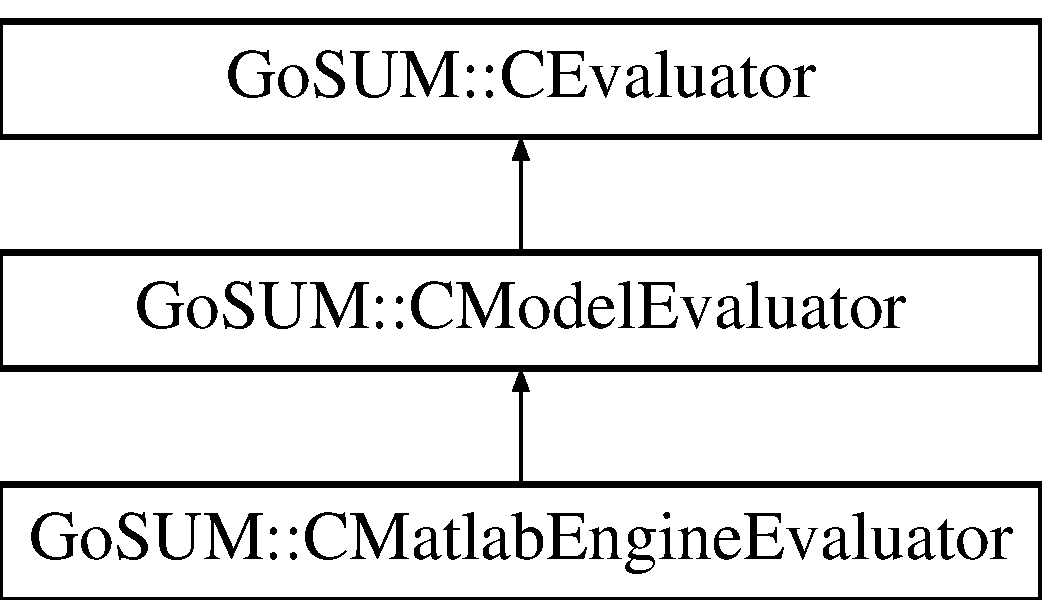
\includegraphics[height=3.000000cm]{class_go_s_u_m_1_1_c_matlab_engine_evaluator}
\end{center}
\end{figure}
\subsection*{Public Member Functions}
\begin{DoxyCompactItemize}
\item 
\hyperlink{class_go_s_u_m_1_1_c_matlab_engine_evaluator_a02ed581900a8c193fa413517e992cce2}{C\-Matlab\-Engine\-Evaluator} ()
\item 
\hyperlink{class_go_s_u_m_1_1_c_matlab_engine_evaluator_af40c36abb8201ffd38ecb9379c04ff36}{C\-Matlab\-Engine\-Evaluator} (const \hyperlink{class_go_s_u_m_1_1_c_input_parameters}{C\-Input\-Parameters} $\ast$\-\_\-p\-I\-P, \hyperlink{class_go_s_u_m_1_1_c_output_states}{C\-Output\-States} $\ast$\-\_\-p\-O\-S, int \-\_\-trd\-I)
\item 
virtual \hyperlink{class_go_s_u_m_1_1_c_matlab_engine_evaluator_a31a086ffbc31094487bed97bbae53bd3}{$\sim$\-C\-Matlab\-Engine\-Evaluator} ()
\item 
virtual void \hyperlink{class_go_s_u_m_1_1_c_matlab_engine_evaluator_a878e5b84a93c808806cad12019372722}{open\-Evaluation} ()
\begin{DoxyCompactList}\small\item\em Opens, i.\-e. prepares evaluation process. \end{DoxyCompactList}\item 
virtual Array\-Xd \hyperlink{class_go_s_u_m_1_1_c_matlab_engine_evaluator_a68cf94eec612bdd72fd032f5631aad66}{operator()} (const Array\-Xd \&X)
\begin{DoxyCompactList}\small\item\em Returns output state evaluated on a single input parameter n-\/tuple. \end{DoxyCompactList}\item 
virtual int \hyperlink{class_go_s_u_m_1_1_c_matlab_engine_evaluator_a646d7c6412cf8256a65271af5b1aad89}{evaluate\-Outputs\-Size} ()
\begin{DoxyCompactList}\small\item\em Evaluates outputs size by running model evaluator. \end{DoxyCompactList}\item 
virtual void \hyperlink{class_go_s_u_m_1_1_c_matlab_engine_evaluator_a238f3a03165e37f5707611ae1e1a53ae}{close\-Evaluation} ()
\begin{DoxyCompactList}\small\item\em Closes evaluation process. \end{DoxyCompactList}\end{DoxyCompactItemize}
\subsection*{Protected Member Functions}
\begin{DoxyCompactItemize}
\item 
{\footnotesize template$<$class Archive $>$ }\\void \hyperlink{class_go_s_u_m_1_1_c_matlab_engine_evaluator_ad33ed3b3581e5da2f7575c0e3f1d9e55}{serialize} (Archive \&ar, const unsigned int version)
\end{DoxyCompactItemize}
\subsection*{Protected Attributes}
\begin{DoxyCompactItemize}
\item 
Engine $\ast$ \hyperlink{class_go_s_u_m_1_1_c_matlab_engine_evaluator_a27f4cdd2025a3dbcc975dc75d8fffb14}{ep}
\begin{DoxyCompactList}\small\item\em Points to the matlab engine. \end{DoxyCompactList}\item 
\hyperlink{class_c_m_a_t_l_a_b}{C\-M\-A\-T\-L\-A\-B} \hyperlink{class_go_s_u_m_1_1_c_matlab_engine_evaluator_ae5cb5436e2edaabb0f0db24d41daac0f}{matlab}
\end{DoxyCompactItemize}
\subsection*{Friends}
\begin{DoxyCompactItemize}
\item 
class \hyperlink{class_go_s_u_m_1_1_c_matlab_engine_evaluator_ac98d07dd8f7b70e16ccb9a01abf56b9c}{boost\-::serialization\-::access}
\begin{DoxyCompactList}\small\item\em Boost serialization. \end{DoxyCompactList}\end{DoxyCompactItemize}
\subsection*{Additional Inherited Members}


\subsection{Detailed Description}
Class for the evaluator through Matlab engine derived from \hyperlink{class_go_s_u_m_1_1_c_model_evaluator}{C\-Model\-Evaluator}. 

\subsection{Constructor \& Destructor Documentation}
\hypertarget{class_go_s_u_m_1_1_c_matlab_engine_evaluator_a02ed581900a8c193fa413517e992cce2}{\index{Go\-S\-U\-M\-::\-C\-Matlab\-Engine\-Evaluator@{Go\-S\-U\-M\-::\-C\-Matlab\-Engine\-Evaluator}!C\-Matlab\-Engine\-Evaluator@{C\-Matlab\-Engine\-Evaluator}}
\index{C\-Matlab\-Engine\-Evaluator@{C\-Matlab\-Engine\-Evaluator}!GoSUM::CMatlabEngineEvaluator@{Go\-S\-U\-M\-::\-C\-Matlab\-Engine\-Evaluator}}
\subsubsection[{C\-Matlab\-Engine\-Evaluator}]{\setlength{\rightskip}{0pt plus 5cm}Go\-S\-U\-M\-::\-C\-Matlab\-Engine\-Evaluator\-::\-C\-Matlab\-Engine\-Evaluator (
\begin{DoxyParamCaption}
{}
\end{DoxyParamCaption}
)\hspace{0.3cm}{\ttfamily [inline]}}}\label{class_go_s_u_m_1_1_c_matlab_engine_evaluator_a02ed581900a8c193fa413517e992cce2}
\hypertarget{class_go_s_u_m_1_1_c_matlab_engine_evaluator_af40c36abb8201ffd38ecb9379c04ff36}{\index{Go\-S\-U\-M\-::\-C\-Matlab\-Engine\-Evaluator@{Go\-S\-U\-M\-::\-C\-Matlab\-Engine\-Evaluator}!C\-Matlab\-Engine\-Evaluator@{C\-Matlab\-Engine\-Evaluator}}
\index{C\-Matlab\-Engine\-Evaluator@{C\-Matlab\-Engine\-Evaluator}!GoSUM::CMatlabEngineEvaluator@{Go\-S\-U\-M\-::\-C\-Matlab\-Engine\-Evaluator}}
\subsubsection[{C\-Matlab\-Engine\-Evaluator}]{\setlength{\rightskip}{0pt plus 5cm}Go\-S\-U\-M\-::\-C\-Matlab\-Engine\-Evaluator\-::\-C\-Matlab\-Engine\-Evaluator (
\begin{DoxyParamCaption}
\item[{const {\bf C\-Input\-Parameters} $\ast$}]{\-\_\-p\-I\-P, }
\item[{{\bf C\-Output\-States} $\ast$}]{\-\_\-p\-O\-S, }
\item[{int}]{\-\_\-trd\-I}
\end{DoxyParamCaption}
)\hspace{0.3cm}{\ttfamily [inline]}}}\label{class_go_s_u_m_1_1_c_matlab_engine_evaluator_af40c36abb8201ffd38ecb9379c04ff36}
\hypertarget{class_go_s_u_m_1_1_c_matlab_engine_evaluator_a31a086ffbc31094487bed97bbae53bd3}{\index{Go\-S\-U\-M\-::\-C\-Matlab\-Engine\-Evaluator@{Go\-S\-U\-M\-::\-C\-Matlab\-Engine\-Evaluator}!$\sim$\-C\-Matlab\-Engine\-Evaluator@{$\sim$\-C\-Matlab\-Engine\-Evaluator}}
\index{$\sim$\-C\-Matlab\-Engine\-Evaluator@{$\sim$\-C\-Matlab\-Engine\-Evaluator}!GoSUM::CMatlabEngineEvaluator@{Go\-S\-U\-M\-::\-C\-Matlab\-Engine\-Evaluator}}
\subsubsection[{$\sim$\-C\-Matlab\-Engine\-Evaluator}]{\setlength{\rightskip}{0pt plus 5cm}virtual Go\-S\-U\-M\-::\-C\-Matlab\-Engine\-Evaluator\-::$\sim$\-C\-Matlab\-Engine\-Evaluator (
\begin{DoxyParamCaption}
{}
\end{DoxyParamCaption}
)\hspace{0.3cm}{\ttfamily [inline]}, {\ttfamily [virtual]}}}\label{class_go_s_u_m_1_1_c_matlab_engine_evaluator_a31a086ffbc31094487bed97bbae53bd3}


\subsection{Member Function Documentation}
\hypertarget{class_go_s_u_m_1_1_c_matlab_engine_evaluator_a238f3a03165e37f5707611ae1e1a53ae}{\index{Go\-S\-U\-M\-::\-C\-Matlab\-Engine\-Evaluator@{Go\-S\-U\-M\-::\-C\-Matlab\-Engine\-Evaluator}!close\-Evaluation@{close\-Evaluation}}
\index{close\-Evaluation@{close\-Evaluation}!GoSUM::CMatlabEngineEvaluator@{Go\-S\-U\-M\-::\-C\-Matlab\-Engine\-Evaluator}}
\subsubsection[{close\-Evaluation}]{\setlength{\rightskip}{0pt plus 5cm}void Go\-S\-U\-M\-::\-C\-Matlab\-Engine\-Evaluator\-::close\-Evaluation (
\begin{DoxyParamCaption}
{}
\end{DoxyParamCaption}
)\hspace{0.3cm}{\ttfamily [virtual]}}}\label{class_go_s_u_m_1_1_c_matlab_engine_evaluator_a238f3a03165e37f5707611ae1e1a53ae}


Closes evaluation process. 



Implements \hyperlink{class_go_s_u_m_1_1_c_model_evaluator_a7ed9761e18560616881ebe459c6b8952}{Go\-S\-U\-M\-::\-C\-Model\-Evaluator}.

\hypertarget{class_go_s_u_m_1_1_c_matlab_engine_evaluator_a646d7c6412cf8256a65271af5b1aad89}{\index{Go\-S\-U\-M\-::\-C\-Matlab\-Engine\-Evaluator@{Go\-S\-U\-M\-::\-C\-Matlab\-Engine\-Evaluator}!evaluate\-Outputs\-Size@{evaluate\-Outputs\-Size}}
\index{evaluate\-Outputs\-Size@{evaluate\-Outputs\-Size}!GoSUM::CMatlabEngineEvaluator@{Go\-S\-U\-M\-::\-C\-Matlab\-Engine\-Evaluator}}
\subsubsection[{evaluate\-Outputs\-Size}]{\setlength{\rightskip}{0pt plus 5cm}int Go\-S\-U\-M\-::\-C\-Matlab\-Engine\-Evaluator\-::evaluate\-Outputs\-Size (
\begin{DoxyParamCaption}
{}
\end{DoxyParamCaption}
)\hspace{0.3cm}{\ttfamily [virtual]}}}\label{class_go_s_u_m_1_1_c_matlab_engine_evaluator_a646d7c6412cf8256a65271af5b1aad89}


Evaluates outputs size by running model evaluator. 



Reimplemented from \hyperlink{class_go_s_u_m_1_1_c_model_evaluator_a822314faa443612c8840e6252018efb2}{Go\-S\-U\-M\-::\-C\-Model\-Evaluator}.

\hypertarget{class_go_s_u_m_1_1_c_matlab_engine_evaluator_a878e5b84a93c808806cad12019372722}{\index{Go\-S\-U\-M\-::\-C\-Matlab\-Engine\-Evaluator@{Go\-S\-U\-M\-::\-C\-Matlab\-Engine\-Evaluator}!open\-Evaluation@{open\-Evaluation}}
\index{open\-Evaluation@{open\-Evaluation}!GoSUM::CMatlabEngineEvaluator@{Go\-S\-U\-M\-::\-C\-Matlab\-Engine\-Evaluator}}
\subsubsection[{open\-Evaluation}]{\setlength{\rightskip}{0pt plus 5cm}void Go\-S\-U\-M\-::\-C\-Matlab\-Engine\-Evaluator\-::open\-Evaluation (
\begin{DoxyParamCaption}
{}
\end{DoxyParamCaption}
)\hspace{0.3cm}{\ttfamily [virtual]}}}\label{class_go_s_u_m_1_1_c_matlab_engine_evaluator_a878e5b84a93c808806cad12019372722}


Opens, i.\-e. prepares evaluation process. 



Implements \hyperlink{class_go_s_u_m_1_1_c_model_evaluator_a0f5afddb7ed75aad687d3a00e44012a0}{Go\-S\-U\-M\-::\-C\-Model\-Evaluator}.

\hypertarget{class_go_s_u_m_1_1_c_matlab_engine_evaluator_a68cf94eec612bdd72fd032f5631aad66}{\index{Go\-S\-U\-M\-::\-C\-Matlab\-Engine\-Evaluator@{Go\-S\-U\-M\-::\-C\-Matlab\-Engine\-Evaluator}!operator()@{operator()}}
\index{operator()@{operator()}!GoSUM::CMatlabEngineEvaluator@{Go\-S\-U\-M\-::\-C\-Matlab\-Engine\-Evaluator}}
\subsubsection[{operator()}]{\setlength{\rightskip}{0pt plus 5cm}Array\-Xd Go\-S\-U\-M\-::\-C\-Matlab\-Engine\-Evaluator\-::operator() (
\begin{DoxyParamCaption}
\item[{const Array\-Xd \&}]{X}
\end{DoxyParamCaption}
)\hspace{0.3cm}{\ttfamily [virtual]}}}\label{class_go_s_u_m_1_1_c_matlab_engine_evaluator_a68cf94eec612bdd72fd032f5631aad66}


Returns output state evaluated on a single input parameter n-\/tuple. 



Implements \hyperlink{class_go_s_u_m_1_1_c_model_evaluator_a17541eada67797802edcae14533361ad}{Go\-S\-U\-M\-::\-C\-Model\-Evaluator}.

\hypertarget{class_go_s_u_m_1_1_c_matlab_engine_evaluator_ad33ed3b3581e5da2f7575c0e3f1d9e55}{\index{Go\-S\-U\-M\-::\-C\-Matlab\-Engine\-Evaluator@{Go\-S\-U\-M\-::\-C\-Matlab\-Engine\-Evaluator}!serialize@{serialize}}
\index{serialize@{serialize}!GoSUM::CMatlabEngineEvaluator@{Go\-S\-U\-M\-::\-C\-Matlab\-Engine\-Evaluator}}
\subsubsection[{serialize}]{\setlength{\rightskip}{0pt plus 5cm}template$<$class Archive $>$ void Go\-S\-U\-M\-::\-C\-Matlab\-Engine\-Evaluator\-::serialize (
\begin{DoxyParamCaption}
\item[{Archive \&}]{ar, }
\item[{const unsigned int}]{version}
\end{DoxyParamCaption}
)\hspace{0.3cm}{\ttfamily [protected]}}}\label{class_go_s_u_m_1_1_c_matlab_engine_evaluator_ad33ed3b3581e5da2f7575c0e3f1d9e55}


Reimplemented from \hyperlink{class_go_s_u_m_1_1_c_model_evaluator_a80e334f1496f3bee1da84cee050a72a1}{Go\-S\-U\-M\-::\-C\-Model\-Evaluator}.



\subsection{Friends And Related Function Documentation}
\hypertarget{class_go_s_u_m_1_1_c_matlab_engine_evaluator_ac98d07dd8f7b70e16ccb9a01abf56b9c}{\index{Go\-S\-U\-M\-::\-C\-Matlab\-Engine\-Evaluator@{Go\-S\-U\-M\-::\-C\-Matlab\-Engine\-Evaluator}!boost\-::serialization\-::access@{boost\-::serialization\-::access}}
\index{boost\-::serialization\-::access@{boost\-::serialization\-::access}!GoSUM::CMatlabEngineEvaluator@{Go\-S\-U\-M\-::\-C\-Matlab\-Engine\-Evaluator}}
\subsubsection[{boost\-::serialization\-::access}]{\setlength{\rightskip}{0pt plus 5cm}friend class boost\-::serialization\-::access\hspace{0.3cm}{\ttfamily [friend]}}}\label{class_go_s_u_m_1_1_c_matlab_engine_evaluator_ac98d07dd8f7b70e16ccb9a01abf56b9c}


Boost serialization. 



\subsection{Member Data Documentation}
\hypertarget{class_go_s_u_m_1_1_c_matlab_engine_evaluator_a27f4cdd2025a3dbcc975dc75d8fffb14}{\index{Go\-S\-U\-M\-::\-C\-Matlab\-Engine\-Evaluator@{Go\-S\-U\-M\-::\-C\-Matlab\-Engine\-Evaluator}!ep@{ep}}
\index{ep@{ep}!GoSUM::CMatlabEngineEvaluator@{Go\-S\-U\-M\-::\-C\-Matlab\-Engine\-Evaluator}}
\subsubsection[{ep}]{\setlength{\rightskip}{0pt plus 5cm}Engine$\ast$ Go\-S\-U\-M\-::\-C\-Matlab\-Engine\-Evaluator\-::ep\hspace{0.3cm}{\ttfamily [protected]}}}\label{class_go_s_u_m_1_1_c_matlab_engine_evaluator_a27f4cdd2025a3dbcc975dc75d8fffb14}


Points to the matlab engine. 

\hypertarget{class_go_s_u_m_1_1_c_matlab_engine_evaluator_ae5cb5436e2edaabb0f0db24d41daac0f}{\index{Go\-S\-U\-M\-::\-C\-Matlab\-Engine\-Evaluator@{Go\-S\-U\-M\-::\-C\-Matlab\-Engine\-Evaluator}!matlab@{matlab}}
\index{matlab@{matlab}!GoSUM::CMatlabEngineEvaluator@{Go\-S\-U\-M\-::\-C\-Matlab\-Engine\-Evaluator}}
\subsubsection[{matlab}]{\setlength{\rightskip}{0pt plus 5cm}{\bf C\-M\-A\-T\-L\-A\-B} Go\-S\-U\-M\-::\-C\-Matlab\-Engine\-Evaluator\-::matlab\hspace{0.3cm}{\ttfamily [protected]}}}\label{class_go_s_u_m_1_1_c_matlab_engine_evaluator_ae5cb5436e2edaabb0f0db24d41daac0f}
Object for matlab library functions. 

The documentation for this class was generated from the following files\-:\begin{DoxyCompactItemize}
\item 
C\-:/\-Development/core/\hyperlink{_original_model_8h}{Original\-Model.\-h}\item 
C\-:/\-Development/core/\hyperlink{_original_model_8cpp}{Original\-Model.\-cpp}\end{DoxyCompactItemize}

\hypertarget{class_go_s_u_m_1_1_c_matlab_shell_evaluator}{\section{Go\-S\-U\-M\-:\-:C\-Matlab\-Shell\-Evaluator Class Reference}
\label{class_go_s_u_m_1_1_c_matlab_shell_evaluator}\index{Go\-S\-U\-M\-::\-C\-Matlab\-Shell\-Evaluator@{Go\-S\-U\-M\-::\-C\-Matlab\-Shell\-Evaluator}}
}


Class for the evaluator through Matlab engine and .mat i/o.  




{\ttfamily \#include $<$Original\-Model.\-h$>$}

Inheritance diagram for Go\-S\-U\-M\-:\-:C\-Matlab\-Shell\-Evaluator\-:\begin{figure}[H]
\begin{center}
\leavevmode
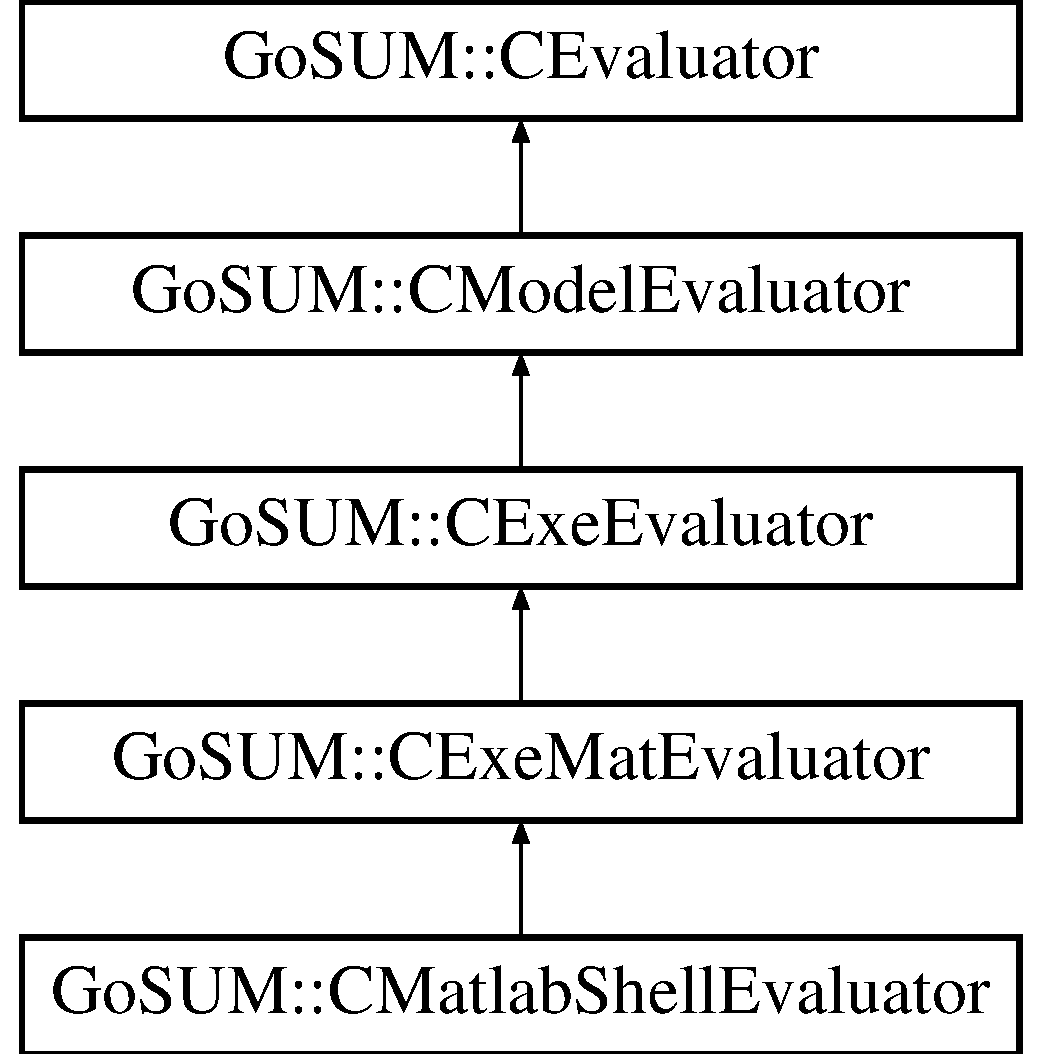
\includegraphics[height=5.000000cm]{class_go_s_u_m_1_1_c_matlab_shell_evaluator}
\end{center}
\end{figure}
\subsection*{Public Member Functions}
\begin{DoxyCompactItemize}
\item 
\hyperlink{class_go_s_u_m_1_1_c_matlab_shell_evaluator_a088aee04655f2158447b5f7631a98ffe}{C\-Matlab\-Shell\-Evaluator} ()
\item 
\hyperlink{class_go_s_u_m_1_1_c_matlab_shell_evaluator_ab7903f6e9ed3ae3fe65321b72552d9f3}{C\-Matlab\-Shell\-Evaluator} (const \hyperlink{class_go_s_u_m_1_1_c_input_parameters}{C\-Input\-Parameters} $\ast$\-\_\-p\-I\-P, \hyperlink{class_go_s_u_m_1_1_c_output_states}{C\-Output\-States} $\ast$\-\_\-p\-O\-S, int \-\_\-trd\-I)
\item 
virtual \hyperlink{class_go_s_u_m_1_1_c_matlab_shell_evaluator_a389f589281db7684ba1671d4ea613f81}{$\sim$\-C\-Matlab\-Shell\-Evaluator} ()
\end{DoxyCompactItemize}
\subsection*{Protected Member Functions}
\begin{DoxyCompactItemize}
\item 
{\footnotesize template$<$class Archive $>$ }\\void \hyperlink{class_go_s_u_m_1_1_c_matlab_shell_evaluator_af84e659441da0694bff64c2d955831b9}{serialize} (Archive \&ar, const unsigned int version)
\item 
virtual void \hyperlink{class_go_s_u_m_1_1_c_matlab_shell_evaluator_ab365048eef74e7b837fcb4420f763f1f}{system\-Command} (std\-::ostringstream \&cmd)
\end{DoxyCompactItemize}
\subsection*{Friends}
\begin{DoxyCompactItemize}
\item 
class \hyperlink{class_go_s_u_m_1_1_c_matlab_shell_evaluator_ac98d07dd8f7b70e16ccb9a01abf56b9c}{boost\-::serialization\-::access}
\begin{DoxyCompactList}\small\item\em Boost serialization. \end{DoxyCompactList}\end{DoxyCompactItemize}
\subsection*{Additional Inherited Members}


\subsection{Detailed Description}
Class for the evaluator through Matlab engine and .mat i/o. 

\subsection{Constructor \& Destructor Documentation}
\hypertarget{class_go_s_u_m_1_1_c_matlab_shell_evaluator_a088aee04655f2158447b5f7631a98ffe}{\index{Go\-S\-U\-M\-::\-C\-Matlab\-Shell\-Evaluator@{Go\-S\-U\-M\-::\-C\-Matlab\-Shell\-Evaluator}!C\-Matlab\-Shell\-Evaluator@{C\-Matlab\-Shell\-Evaluator}}
\index{C\-Matlab\-Shell\-Evaluator@{C\-Matlab\-Shell\-Evaluator}!GoSUM::CMatlabShellEvaluator@{Go\-S\-U\-M\-::\-C\-Matlab\-Shell\-Evaluator}}
\subsubsection[{C\-Matlab\-Shell\-Evaluator}]{\setlength{\rightskip}{0pt plus 5cm}Go\-S\-U\-M\-::\-C\-Matlab\-Shell\-Evaluator\-::\-C\-Matlab\-Shell\-Evaluator (
\begin{DoxyParamCaption}
{}
\end{DoxyParamCaption}
)\hspace{0.3cm}{\ttfamily [inline]}}}\label{class_go_s_u_m_1_1_c_matlab_shell_evaluator_a088aee04655f2158447b5f7631a98ffe}
\hypertarget{class_go_s_u_m_1_1_c_matlab_shell_evaluator_ab7903f6e9ed3ae3fe65321b72552d9f3}{\index{Go\-S\-U\-M\-::\-C\-Matlab\-Shell\-Evaluator@{Go\-S\-U\-M\-::\-C\-Matlab\-Shell\-Evaluator}!C\-Matlab\-Shell\-Evaluator@{C\-Matlab\-Shell\-Evaluator}}
\index{C\-Matlab\-Shell\-Evaluator@{C\-Matlab\-Shell\-Evaluator}!GoSUM::CMatlabShellEvaluator@{Go\-S\-U\-M\-::\-C\-Matlab\-Shell\-Evaluator}}
\subsubsection[{C\-Matlab\-Shell\-Evaluator}]{\setlength{\rightskip}{0pt plus 5cm}Go\-S\-U\-M\-::\-C\-Matlab\-Shell\-Evaluator\-::\-C\-Matlab\-Shell\-Evaluator (
\begin{DoxyParamCaption}
\item[{const {\bf C\-Input\-Parameters} $\ast$}]{\-\_\-p\-I\-P, }
\item[{{\bf C\-Output\-States} $\ast$}]{\-\_\-p\-O\-S, }
\item[{int}]{\-\_\-trd\-I}
\end{DoxyParamCaption}
)\hspace{0.3cm}{\ttfamily [inline]}}}\label{class_go_s_u_m_1_1_c_matlab_shell_evaluator_ab7903f6e9ed3ae3fe65321b72552d9f3}
\hypertarget{class_go_s_u_m_1_1_c_matlab_shell_evaluator_a389f589281db7684ba1671d4ea613f81}{\index{Go\-S\-U\-M\-::\-C\-Matlab\-Shell\-Evaluator@{Go\-S\-U\-M\-::\-C\-Matlab\-Shell\-Evaluator}!$\sim$\-C\-Matlab\-Shell\-Evaluator@{$\sim$\-C\-Matlab\-Shell\-Evaluator}}
\index{$\sim$\-C\-Matlab\-Shell\-Evaluator@{$\sim$\-C\-Matlab\-Shell\-Evaluator}!GoSUM::CMatlabShellEvaluator@{Go\-S\-U\-M\-::\-C\-Matlab\-Shell\-Evaluator}}
\subsubsection[{$\sim$\-C\-Matlab\-Shell\-Evaluator}]{\setlength{\rightskip}{0pt plus 5cm}virtual Go\-S\-U\-M\-::\-C\-Matlab\-Shell\-Evaluator\-::$\sim$\-C\-Matlab\-Shell\-Evaluator (
\begin{DoxyParamCaption}
{}
\end{DoxyParamCaption}
)\hspace{0.3cm}{\ttfamily [inline]}, {\ttfamily [virtual]}}}\label{class_go_s_u_m_1_1_c_matlab_shell_evaluator_a389f589281db7684ba1671d4ea613f81}


\subsection{Member Function Documentation}
\hypertarget{class_go_s_u_m_1_1_c_matlab_shell_evaluator_af84e659441da0694bff64c2d955831b9}{\index{Go\-S\-U\-M\-::\-C\-Matlab\-Shell\-Evaluator@{Go\-S\-U\-M\-::\-C\-Matlab\-Shell\-Evaluator}!serialize@{serialize}}
\index{serialize@{serialize}!GoSUM::CMatlabShellEvaluator@{Go\-S\-U\-M\-::\-C\-Matlab\-Shell\-Evaluator}}
\subsubsection[{serialize}]{\setlength{\rightskip}{0pt plus 5cm}template$<$class Archive $>$ void Go\-S\-U\-M\-::\-C\-Matlab\-Shell\-Evaluator\-::serialize (
\begin{DoxyParamCaption}
\item[{Archive \&}]{ar, }
\item[{const unsigned int}]{version}
\end{DoxyParamCaption}
)\hspace{0.3cm}{\ttfamily [protected]}}}\label{class_go_s_u_m_1_1_c_matlab_shell_evaluator_af84e659441da0694bff64c2d955831b9}


Reimplemented from \hyperlink{class_go_s_u_m_1_1_c_exe_mat_evaluator_a2e5121b751aaeb6f5c805cfe0312c20d}{Go\-S\-U\-M\-::\-C\-Exe\-Mat\-Evaluator}.

\hypertarget{class_go_s_u_m_1_1_c_matlab_shell_evaluator_ab365048eef74e7b837fcb4420f763f1f}{\index{Go\-S\-U\-M\-::\-C\-Matlab\-Shell\-Evaluator@{Go\-S\-U\-M\-::\-C\-Matlab\-Shell\-Evaluator}!system\-Command@{system\-Command}}
\index{system\-Command@{system\-Command}!GoSUM::CMatlabShellEvaluator@{Go\-S\-U\-M\-::\-C\-Matlab\-Shell\-Evaluator}}
\subsubsection[{system\-Command}]{\setlength{\rightskip}{0pt plus 5cm}virtual void Go\-S\-U\-M\-::\-C\-Matlab\-Shell\-Evaluator\-::system\-Command (
\begin{DoxyParamCaption}
\item[{std\-::ostringstream \&}]{cmd}
\end{DoxyParamCaption}
)\hspace{0.3cm}{\ttfamily [inline]}, {\ttfamily [protected]}, {\ttfamily [virtual]}}}\label{class_go_s_u_m_1_1_c_matlab_shell_evaluator_ab365048eef74e7b837fcb4420f763f1f}


Reimplemented from \hyperlink{class_go_s_u_m_1_1_c_exe_evaluator_aeb6c371d09cbc3cb3a0152779a32bf52}{Go\-S\-U\-M\-::\-C\-Exe\-Evaluator}.



\subsection{Friends And Related Function Documentation}
\hypertarget{class_go_s_u_m_1_1_c_matlab_shell_evaluator_ac98d07dd8f7b70e16ccb9a01abf56b9c}{\index{Go\-S\-U\-M\-::\-C\-Matlab\-Shell\-Evaluator@{Go\-S\-U\-M\-::\-C\-Matlab\-Shell\-Evaluator}!boost\-::serialization\-::access@{boost\-::serialization\-::access}}
\index{boost\-::serialization\-::access@{boost\-::serialization\-::access}!GoSUM::CMatlabShellEvaluator@{Go\-S\-U\-M\-::\-C\-Matlab\-Shell\-Evaluator}}
\subsubsection[{boost\-::serialization\-::access}]{\setlength{\rightskip}{0pt plus 5cm}friend class boost\-::serialization\-::access\hspace{0.3cm}{\ttfamily [friend]}}}\label{class_go_s_u_m_1_1_c_matlab_shell_evaluator_ac98d07dd8f7b70e16ccb9a01abf56b9c}


Boost serialization. 



The documentation for this class was generated from the following files\-:\begin{DoxyCompactItemize}
\item 
C\-:/\-Development/core/\hyperlink{_original_model_8h}{Original\-Model.\-h}\item 
C\-:/\-Development/core/\hyperlink{_original_model_8cpp}{Original\-Model.\-cpp}\end{DoxyCompactItemize}

\hypertarget{class_c_medium_period_r_n_g}{\section{C\-Medium\-Period\-R\-N\-G Class Reference}
\label{class_c_medium_period_r_n_g}\index{C\-Medium\-Period\-R\-N\-G@{C\-Medium\-Period\-R\-N\-G}}
}


{\ttfamily \#include $<$Random\-Generators.\-h$>$}

Inheritance diagram for C\-Medium\-Period\-R\-N\-G\-:\begin{figure}[H]
\begin{center}
\leavevmode
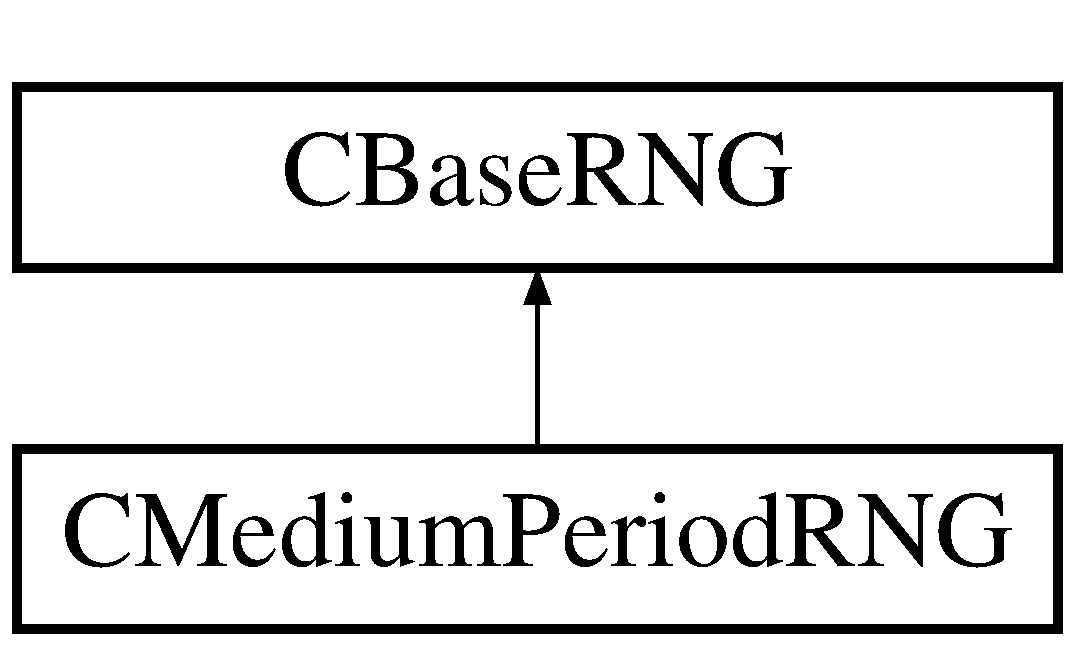
\includegraphics[height=2.000000cm]{class_c_medium_period_r_n_g}
\end{center}
\end{figure}
\subsection*{Public Member Functions}
\begin{DoxyCompactItemize}
\item 
\hyperlink{class_c_medium_period_r_n_g_aba95f9e5dcb09e40c95801d404819c40}{C\-Medium\-Period\-R\-N\-G} ()
\item 
\hyperlink{class_c_medium_period_r_n_g_a26abf9707201f8ca9bbb4643970546ac}{C\-Medium\-Period\-R\-N\-G} (unsigned int s)
\item 
virtual \hyperlink{class_c_medium_period_r_n_g_a7a115251a984445fa5e2f5a8d8bda0af}{$\sim$\-C\-Medium\-Period\-R\-N\-G} ()
\item 
virtual void \hyperlink{class_c_medium_period_r_n_g_a8f0a3aebcea30b879719d9af1ac548e1}{set\-Seed} (unsigned int s)
\begin{DoxyCompactList}\small\item\em Sets seed of the R\-N\-G. \end{DoxyCompactList}\item 
virtual unsigned int \hyperlink{class_c_medium_period_r_n_g_a12611a6c74a312860cccfbdb2bdbf89e}{rndi} ()
\begin{DoxyCompactList}\small\item\em Returns randomly generated unsigned int. \end{DoxyCompactList}\item 
virtual double \hyperlink{class_c_medium_period_r_n_g_a56a6e5751b8563b56c30f5c1d0351eec}{rnd} ()
\begin{DoxyCompactList}\small\item\em Returns randomly generated double between 0 and 1. \end{DoxyCompactList}\end{DoxyCompactItemize}
\subsection*{Static Private Attributes}
\begin{DoxyCompactItemize}
\item 
static long \hyperlink{class_c_medium_period_r_n_g_a15dda956071d7e8874502761029e37ed}{idum2} = 123456789
\begin{DoxyCompactList}\small\item\em Paramters of the medium period R\-N\-G. \end{DoxyCompactList}\item 
static long \hyperlink{class_c_medium_period_r_n_g_a1da6d94f9e9e3fe4b83f9a6ae3c81825}{iy2} = 0
\begin{DoxyCompactList}\small\item\em Paramters of the medium period R\-N\-G. \end{DoxyCompactList}\item 
static long \hyperlink{class_c_medium_period_r_n_g_ad6be479584d3d21455f253a8254221c4}{iv2} \mbox{[}\hyperlink{_random_generators_8h_a0e93cfb2d62849853fd34957ba6e6fdc}{N\-T\-A\-B}\mbox{]}
\begin{DoxyCompactList}\small\item\em Paramters of the medium period R\-N\-G. \end{DoxyCompactList}\item 
static long \hyperlink{class_c_medium_period_r_n_g_aae9ed6044330aabad8e3571ac483800d}{idum} = 0
\begin{DoxyCompactList}\small\item\em Paramters of the medium period R\-N\-G. \end{DoxyCompactList}\end{DoxyCompactItemize}


\subsection{Constructor \& Destructor Documentation}
\hypertarget{class_c_medium_period_r_n_g_aba95f9e5dcb09e40c95801d404819c40}{\index{C\-Medium\-Period\-R\-N\-G@{C\-Medium\-Period\-R\-N\-G}!C\-Medium\-Period\-R\-N\-G@{C\-Medium\-Period\-R\-N\-G}}
\index{C\-Medium\-Period\-R\-N\-G@{C\-Medium\-Period\-R\-N\-G}!CMediumPeriodRNG@{C\-Medium\-Period\-R\-N\-G}}
\subsubsection[{C\-Medium\-Period\-R\-N\-G}]{\setlength{\rightskip}{0pt plus 5cm}C\-Medium\-Period\-R\-N\-G\-::\-C\-Medium\-Period\-R\-N\-G (
\begin{DoxyParamCaption}
{}
\end{DoxyParamCaption}
)\hspace{0.3cm}{\ttfamily [inline]}}}\label{class_c_medium_period_r_n_g_aba95f9e5dcb09e40c95801d404819c40}
\hypertarget{class_c_medium_period_r_n_g_a26abf9707201f8ca9bbb4643970546ac}{\index{C\-Medium\-Period\-R\-N\-G@{C\-Medium\-Period\-R\-N\-G}!C\-Medium\-Period\-R\-N\-G@{C\-Medium\-Period\-R\-N\-G}}
\index{C\-Medium\-Period\-R\-N\-G@{C\-Medium\-Period\-R\-N\-G}!CMediumPeriodRNG@{C\-Medium\-Period\-R\-N\-G}}
\subsubsection[{C\-Medium\-Period\-R\-N\-G}]{\setlength{\rightskip}{0pt plus 5cm}C\-Medium\-Period\-R\-N\-G\-::\-C\-Medium\-Period\-R\-N\-G (
\begin{DoxyParamCaption}
\item[{unsigned int}]{s}
\end{DoxyParamCaption}
)\hspace{0.3cm}{\ttfamily [inline]}}}\label{class_c_medium_period_r_n_g_a26abf9707201f8ca9bbb4643970546ac}
\hypertarget{class_c_medium_period_r_n_g_a7a115251a984445fa5e2f5a8d8bda0af}{\index{C\-Medium\-Period\-R\-N\-G@{C\-Medium\-Period\-R\-N\-G}!$\sim$\-C\-Medium\-Period\-R\-N\-G@{$\sim$\-C\-Medium\-Period\-R\-N\-G}}
\index{$\sim$\-C\-Medium\-Period\-R\-N\-G@{$\sim$\-C\-Medium\-Period\-R\-N\-G}!CMediumPeriodRNG@{C\-Medium\-Period\-R\-N\-G}}
\subsubsection[{$\sim$\-C\-Medium\-Period\-R\-N\-G}]{\setlength{\rightskip}{0pt plus 5cm}virtual C\-Medium\-Period\-R\-N\-G\-::$\sim$\-C\-Medium\-Period\-R\-N\-G (
\begin{DoxyParamCaption}
{}
\end{DoxyParamCaption}
)\hspace{0.3cm}{\ttfamily [inline]}, {\ttfamily [virtual]}}}\label{class_c_medium_period_r_n_g_a7a115251a984445fa5e2f5a8d8bda0af}


\subsection{Member Function Documentation}
\hypertarget{class_c_medium_period_r_n_g_a56a6e5751b8563b56c30f5c1d0351eec}{\index{C\-Medium\-Period\-R\-N\-G@{C\-Medium\-Period\-R\-N\-G}!rnd@{rnd}}
\index{rnd@{rnd}!CMediumPeriodRNG@{C\-Medium\-Period\-R\-N\-G}}
\subsubsection[{rnd}]{\setlength{\rightskip}{0pt plus 5cm}double C\-Medium\-Period\-R\-N\-G\-::rnd (
\begin{DoxyParamCaption}
{}
\end{DoxyParamCaption}
)\hspace{0.3cm}{\ttfamily [virtual]}}}\label{class_c_medium_period_r_n_g_a56a6e5751b8563b56c30f5c1d0351eec}


Returns randomly generated double between 0 and 1. 



Implements \hyperlink{class_c_base_r_n_g_abbd60a5ecdc9502dd646434224ab5d6b}{C\-Base\-R\-N\-G}.

\hypertarget{class_c_medium_period_r_n_g_a12611a6c74a312860cccfbdb2bdbf89e}{\index{C\-Medium\-Period\-R\-N\-G@{C\-Medium\-Period\-R\-N\-G}!rndi@{rndi}}
\index{rndi@{rndi}!CMediumPeriodRNG@{C\-Medium\-Period\-R\-N\-G}}
\subsubsection[{rndi}]{\setlength{\rightskip}{0pt plus 5cm}virtual unsigned int C\-Medium\-Period\-R\-N\-G\-::rndi (
\begin{DoxyParamCaption}
{}
\end{DoxyParamCaption}
)\hspace{0.3cm}{\ttfamily [inline]}, {\ttfamily [virtual]}}}\label{class_c_medium_period_r_n_g_a12611a6c74a312860cccfbdb2bdbf89e}


Returns randomly generated unsigned int. 



Implements \hyperlink{class_c_base_r_n_g_a2db96fbf06a2f11b3613d422043fb7b8}{C\-Base\-R\-N\-G}.

\hypertarget{class_c_medium_period_r_n_g_a8f0a3aebcea30b879719d9af1ac548e1}{\index{C\-Medium\-Period\-R\-N\-G@{C\-Medium\-Period\-R\-N\-G}!set\-Seed@{set\-Seed}}
\index{set\-Seed@{set\-Seed}!CMediumPeriodRNG@{C\-Medium\-Period\-R\-N\-G}}
\subsubsection[{set\-Seed}]{\setlength{\rightskip}{0pt plus 5cm}void C\-Medium\-Period\-R\-N\-G\-::set\-Seed (
\begin{DoxyParamCaption}
\item[{unsigned int}]{s}
\end{DoxyParamCaption}
)\hspace{0.3cm}{\ttfamily [virtual]}}}\label{class_c_medium_period_r_n_g_a8f0a3aebcea30b879719d9af1ac548e1}


Sets seed of the R\-N\-G. 



Implements \hyperlink{class_c_base_r_n_g_a56fbf75ca07b73954596ee04820e0b07}{C\-Base\-R\-N\-G}.



\subsection{Member Data Documentation}
\hypertarget{class_c_medium_period_r_n_g_aae9ed6044330aabad8e3571ac483800d}{\index{C\-Medium\-Period\-R\-N\-G@{C\-Medium\-Period\-R\-N\-G}!idum@{idum}}
\index{idum@{idum}!CMediumPeriodRNG@{C\-Medium\-Period\-R\-N\-G}}
\subsubsection[{idum}]{\setlength{\rightskip}{0pt plus 5cm}long C\-Medium\-Period\-R\-N\-G\-::idum = 0\hspace{0.3cm}{\ttfamily [static]}, {\ttfamily [private]}}}\label{class_c_medium_period_r_n_g_aae9ed6044330aabad8e3571ac483800d}


Paramters of the medium period R\-N\-G. 

\hypertarget{class_c_medium_period_r_n_g_a15dda956071d7e8874502761029e37ed}{\index{C\-Medium\-Period\-R\-N\-G@{C\-Medium\-Period\-R\-N\-G}!idum2@{idum2}}
\index{idum2@{idum2}!CMediumPeriodRNG@{C\-Medium\-Period\-R\-N\-G}}
\subsubsection[{idum2}]{\setlength{\rightskip}{0pt plus 5cm}long C\-Medium\-Period\-R\-N\-G\-::idum2 = 123456789\hspace{0.3cm}{\ttfamily [static]}, {\ttfamily [private]}}}\label{class_c_medium_period_r_n_g_a15dda956071d7e8874502761029e37ed}


Paramters of the medium period R\-N\-G. 

\hypertarget{class_c_medium_period_r_n_g_ad6be479584d3d21455f253a8254221c4}{\index{C\-Medium\-Period\-R\-N\-G@{C\-Medium\-Period\-R\-N\-G}!iv2@{iv2}}
\index{iv2@{iv2}!CMediumPeriodRNG@{C\-Medium\-Period\-R\-N\-G}}
\subsubsection[{iv2}]{\setlength{\rightskip}{0pt plus 5cm}long C\-Medium\-Period\-R\-N\-G\-::iv2\hspace{0.3cm}{\ttfamily [static]}, {\ttfamily [private]}}}\label{class_c_medium_period_r_n_g_ad6be479584d3d21455f253a8254221c4}


Paramters of the medium period R\-N\-G. 

\hypertarget{class_c_medium_period_r_n_g_a1da6d94f9e9e3fe4b83f9a6ae3c81825}{\index{C\-Medium\-Period\-R\-N\-G@{C\-Medium\-Period\-R\-N\-G}!iy2@{iy2}}
\index{iy2@{iy2}!CMediumPeriodRNG@{C\-Medium\-Period\-R\-N\-G}}
\subsubsection[{iy2}]{\setlength{\rightskip}{0pt plus 5cm}long C\-Medium\-Period\-R\-N\-G\-::iy2 = 0\hspace{0.3cm}{\ttfamily [static]}, {\ttfamily [private]}}}\label{class_c_medium_period_r_n_g_a1da6d94f9e9e3fe4b83f9a6ae3c81825}


Paramters of the medium period R\-N\-G. 



The documentation for this class was generated from the following files\-:\begin{DoxyCompactItemize}
\item 
C\-:/\-Development/core/\hyperlink{_random_generators_8h}{Random\-Generators.\-h}\item 
C\-:/\-Development/core/\hyperlink{_random_generators_8cpp}{Random\-Generators.\-cpp}\end{DoxyCompactItemize}

\hypertarget{class_go_s_u_m_1_1_c_model_constraints}{\section{Go\-S\-U\-M\-:\-:C\-Model\-Constraints Class Reference}
\label{class_go_s_u_m_1_1_c_model_constraints}\index{Go\-S\-U\-M\-::\-C\-Model\-Constraints@{Go\-S\-U\-M\-::\-C\-Model\-Constraints}}
}


{\ttfamily \#include $<$Constraints.\-h$>$}

Inheritance diagram for Go\-S\-U\-M\-:\-:C\-Model\-Constraints\-:\begin{figure}[H]
\begin{center}
\leavevmode
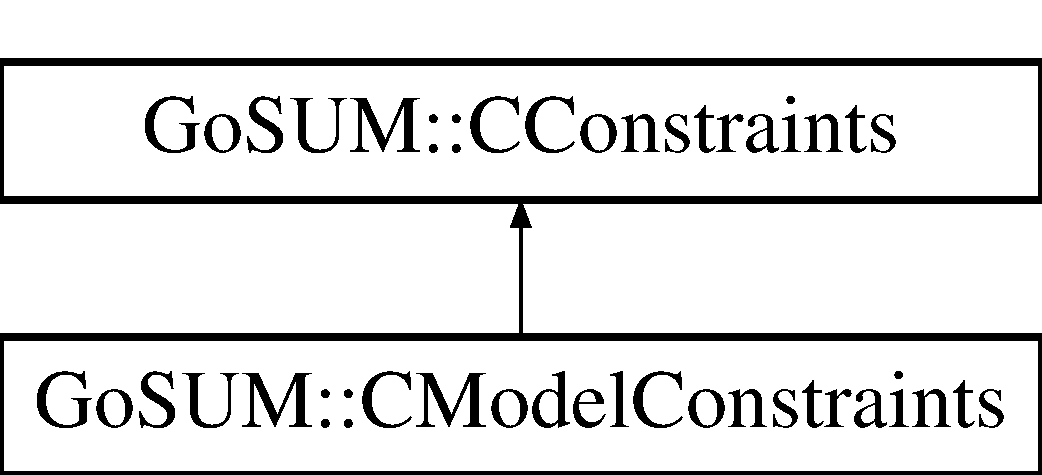
\includegraphics[height=2.000000cm]{class_go_s_u_m_1_1_c_model_constraints}
\end{center}
\end{figure}
\subsection*{Public Member Functions}
\begin{DoxyCompactItemize}
\item 
\hyperlink{class_go_s_u_m_1_1_c_model_constraints_a1d6d718ab8ceeef75a4e35bbc747ccba}{C\-Model\-Constraints} ()
\item 
virtual \hyperlink{class_go_s_u_m_1_1_c_model_constraints_a903d48132b0bc708f1ae4c72bb1f1223}{$\sim$\-C\-Model\-Constraints} ()
\item 
virtual void \hyperlink{class_go_s_u_m_1_1_c_model_constraints_ab547fb9c0109eb85715d65caf04eed84}{clear} ()
\begin{DoxyCompactList}\small\item\em Clears object. \end{DoxyCompactList}\item 
void \hyperlink{class_go_s_u_m_1_1_c_model_constraints_a0191da2921b3dd708e7aa5466735402b}{set} (\hyperlink{class_go_s_u_m_1_1_c_input_parameters}{C\-Input\-Parameters} $\ast$\-\_\-p\-I\-P)
\begin{DoxyCompactList}\small\item\em Sets input parameters pointer. \end{DoxyCompactList}\item 
bool \hyperlink{class_go_s_u_m_1_1_c_model_constraints_a3b6c33a11d19b7efc0f293fb1252bae8}{is\-Constrained} (int \-\_\-at) const 
\begin{DoxyCompactList}\small\item\em Returns status (cosntrained or not) for particular input parameter. \end{DoxyCompactList}\end{DoxyCompactItemize}
\subsection*{Protected Member Functions}
\begin{DoxyCompactItemize}
\item 
{\footnotesize template$<$class Archive $>$ }\\void \hyperlink{class_go_s_u_m_1_1_c_model_constraints_a7e4ec6b59419b56907b7cfedec230ca7}{serialize} (Archive \&ar, const unsigned int version)
\item 
virtual void \hyperlink{class_go_s_u_m_1_1_c_model_constraints_afe8e8cbf1fc08ae1f2ee494146da01fa}{set\-Variable\-Names} ()
\begin{DoxyCompactList}\small\item\em Sets variable names for the parser. \end{DoxyCompactList}\end{DoxyCompactItemize}
\subsection*{Protected Attributes}
\begin{DoxyCompactItemize}
\item 
\hyperlink{class_go_s_u_m_1_1_c_input_parameters}{C\-Input\-Parameters} $\ast$ \hyperlink{class_go_s_u_m_1_1_c_model_constraints_a174e787472c4043054393c0bb5aaf402}{p\-I\-P}
\begin{DoxyCompactList}\small\item\em Points to input parameters. \end{DoxyCompactList}\item 
std\-::vector$<$ bool $>$ \hyperlink{class_go_s_u_m_1_1_c_model_constraints_a499e59d8384b98eaba5498043e792f26}{status}
\end{DoxyCompactItemize}
\subsection*{Friends}
\begin{DoxyCompactItemize}
\item 
class \hyperlink{class_go_s_u_m_1_1_c_model_constraints_ac98d07dd8f7b70e16ccb9a01abf56b9c}{boost\-::serialization\-::access}
\begin{DoxyCompactList}\small\item\em Boost serialization. \end{DoxyCompactList}\end{DoxyCompactItemize}


\subsection{Constructor \& Destructor Documentation}
\hypertarget{class_go_s_u_m_1_1_c_model_constraints_a1d6d718ab8ceeef75a4e35bbc747ccba}{\index{Go\-S\-U\-M\-::\-C\-Model\-Constraints@{Go\-S\-U\-M\-::\-C\-Model\-Constraints}!C\-Model\-Constraints@{C\-Model\-Constraints}}
\index{C\-Model\-Constraints@{C\-Model\-Constraints}!GoSUM::CModelConstraints@{Go\-S\-U\-M\-::\-C\-Model\-Constraints}}
\subsubsection[{C\-Model\-Constraints}]{\setlength{\rightskip}{0pt plus 5cm}Go\-S\-U\-M\-::\-C\-Model\-Constraints\-::\-C\-Model\-Constraints (
\begin{DoxyParamCaption}
{}
\end{DoxyParamCaption}
)\hspace{0.3cm}{\ttfamily [inline]}}}\label{class_go_s_u_m_1_1_c_model_constraints_a1d6d718ab8ceeef75a4e35bbc747ccba}
\hypertarget{class_go_s_u_m_1_1_c_model_constraints_a903d48132b0bc708f1ae4c72bb1f1223}{\index{Go\-S\-U\-M\-::\-C\-Model\-Constraints@{Go\-S\-U\-M\-::\-C\-Model\-Constraints}!$\sim$\-C\-Model\-Constraints@{$\sim$\-C\-Model\-Constraints}}
\index{$\sim$\-C\-Model\-Constraints@{$\sim$\-C\-Model\-Constraints}!GoSUM::CModelConstraints@{Go\-S\-U\-M\-::\-C\-Model\-Constraints}}
\subsubsection[{$\sim$\-C\-Model\-Constraints}]{\setlength{\rightskip}{0pt plus 5cm}virtual Go\-S\-U\-M\-::\-C\-Model\-Constraints\-::$\sim$\-C\-Model\-Constraints (
\begin{DoxyParamCaption}
{}
\end{DoxyParamCaption}
)\hspace{0.3cm}{\ttfamily [inline]}, {\ttfamily [virtual]}}}\label{class_go_s_u_m_1_1_c_model_constraints_a903d48132b0bc708f1ae4c72bb1f1223}


\subsection{Member Function Documentation}
\hypertarget{class_go_s_u_m_1_1_c_model_constraints_ab547fb9c0109eb85715d65caf04eed84}{\index{Go\-S\-U\-M\-::\-C\-Model\-Constraints@{Go\-S\-U\-M\-::\-C\-Model\-Constraints}!clear@{clear}}
\index{clear@{clear}!GoSUM::CModelConstraints@{Go\-S\-U\-M\-::\-C\-Model\-Constraints}}
\subsubsection[{clear}]{\setlength{\rightskip}{0pt plus 5cm}virtual void Go\-S\-U\-M\-::\-C\-Model\-Constraints\-::clear (
\begin{DoxyParamCaption}
{}
\end{DoxyParamCaption}
)\hspace{0.3cm}{\ttfamily [inline]}, {\ttfamily [virtual]}}}\label{class_go_s_u_m_1_1_c_model_constraints_ab547fb9c0109eb85715d65caf04eed84}


Clears object. 



Reimplemented from \hyperlink{class_go_s_u_m_1_1_c_constraints_a45acde7b103ba957a718031b6ecebf69}{Go\-S\-U\-M\-::\-C\-Constraints}.

\hypertarget{class_go_s_u_m_1_1_c_model_constraints_a3b6c33a11d19b7efc0f293fb1252bae8}{\index{Go\-S\-U\-M\-::\-C\-Model\-Constraints@{Go\-S\-U\-M\-::\-C\-Model\-Constraints}!is\-Constrained@{is\-Constrained}}
\index{is\-Constrained@{is\-Constrained}!GoSUM::CModelConstraints@{Go\-S\-U\-M\-::\-C\-Model\-Constraints}}
\subsubsection[{is\-Constrained}]{\setlength{\rightskip}{0pt plus 5cm}bool Go\-S\-U\-M\-::\-C\-Model\-Constraints\-::is\-Constrained (
\begin{DoxyParamCaption}
\item[{int}]{\-\_\-at}
\end{DoxyParamCaption}
) const\hspace{0.3cm}{\ttfamily [inline]}}}\label{class_go_s_u_m_1_1_c_model_constraints_a3b6c33a11d19b7efc0f293fb1252bae8}


Returns status (cosntrained or not) for particular input parameter. 

\hypertarget{class_go_s_u_m_1_1_c_model_constraints_a7e4ec6b59419b56907b7cfedec230ca7}{\index{Go\-S\-U\-M\-::\-C\-Model\-Constraints@{Go\-S\-U\-M\-::\-C\-Model\-Constraints}!serialize@{serialize}}
\index{serialize@{serialize}!GoSUM::CModelConstraints@{Go\-S\-U\-M\-::\-C\-Model\-Constraints}}
\subsubsection[{serialize}]{\setlength{\rightskip}{0pt plus 5cm}template$<$class Archive $>$ void Go\-S\-U\-M\-::\-C\-Model\-Constraints\-::serialize (
\begin{DoxyParamCaption}
\item[{Archive \&}]{ar, }
\item[{const unsigned int}]{version}
\end{DoxyParamCaption}
)\hspace{0.3cm}{\ttfamily [protected]}}}\label{class_go_s_u_m_1_1_c_model_constraints_a7e4ec6b59419b56907b7cfedec230ca7}


Reimplemented from \hyperlink{class_go_s_u_m_1_1_c_constraints_af98bbd20b50e8db2b88630d865fbf10f}{Go\-S\-U\-M\-::\-C\-Constraints}.

\hypertarget{class_go_s_u_m_1_1_c_model_constraints_a0191da2921b3dd708e7aa5466735402b}{\index{Go\-S\-U\-M\-::\-C\-Model\-Constraints@{Go\-S\-U\-M\-::\-C\-Model\-Constraints}!set@{set}}
\index{set@{set}!GoSUM::CModelConstraints@{Go\-S\-U\-M\-::\-C\-Model\-Constraints}}
\subsubsection[{set}]{\setlength{\rightskip}{0pt plus 5cm}void Go\-S\-U\-M\-::\-C\-Model\-Constraints\-::set (
\begin{DoxyParamCaption}
\item[{{\bf C\-Input\-Parameters} $\ast$}]{\-\_\-p\-I\-P}
\end{DoxyParamCaption}
)}}\label{class_go_s_u_m_1_1_c_model_constraints_a0191da2921b3dd708e7aa5466735402b}


Sets input parameters pointer. 

\hypertarget{class_go_s_u_m_1_1_c_model_constraints_afe8e8cbf1fc08ae1f2ee494146da01fa}{\index{Go\-S\-U\-M\-::\-C\-Model\-Constraints@{Go\-S\-U\-M\-::\-C\-Model\-Constraints}!set\-Variable\-Names@{set\-Variable\-Names}}
\index{set\-Variable\-Names@{set\-Variable\-Names}!GoSUM::CModelConstraints@{Go\-S\-U\-M\-::\-C\-Model\-Constraints}}
\subsubsection[{set\-Variable\-Names}]{\setlength{\rightskip}{0pt plus 5cm}void Go\-S\-U\-M\-::\-C\-Model\-Constraints\-::set\-Variable\-Names (
\begin{DoxyParamCaption}
{}
\end{DoxyParamCaption}
)\hspace{0.3cm}{\ttfamily [protected]}, {\ttfamily [virtual]}}}\label{class_go_s_u_m_1_1_c_model_constraints_afe8e8cbf1fc08ae1f2ee494146da01fa}


Sets variable names for the parser. 



Implements \hyperlink{class_go_s_u_m_1_1_c_constraints_a68a322c212879db65e3ebc1c1f201432}{Go\-S\-U\-M\-::\-C\-Constraints}.



\subsection{Friends And Related Function Documentation}
\hypertarget{class_go_s_u_m_1_1_c_model_constraints_ac98d07dd8f7b70e16ccb9a01abf56b9c}{\index{Go\-S\-U\-M\-::\-C\-Model\-Constraints@{Go\-S\-U\-M\-::\-C\-Model\-Constraints}!boost\-::serialization\-::access@{boost\-::serialization\-::access}}
\index{boost\-::serialization\-::access@{boost\-::serialization\-::access}!GoSUM::CModelConstraints@{Go\-S\-U\-M\-::\-C\-Model\-Constraints}}
\subsubsection[{boost\-::serialization\-::access}]{\setlength{\rightskip}{0pt plus 5cm}friend class boost\-::serialization\-::access\hspace{0.3cm}{\ttfamily [friend]}}}\label{class_go_s_u_m_1_1_c_model_constraints_ac98d07dd8f7b70e16ccb9a01abf56b9c}


Boost serialization. 



\subsection{Member Data Documentation}
\hypertarget{class_go_s_u_m_1_1_c_model_constraints_a174e787472c4043054393c0bb5aaf402}{\index{Go\-S\-U\-M\-::\-C\-Model\-Constraints@{Go\-S\-U\-M\-::\-C\-Model\-Constraints}!p\-I\-P@{p\-I\-P}}
\index{p\-I\-P@{p\-I\-P}!GoSUM::CModelConstraints@{Go\-S\-U\-M\-::\-C\-Model\-Constraints}}
\subsubsection[{p\-I\-P}]{\setlength{\rightskip}{0pt plus 5cm}{\bf C\-Input\-Parameters}$\ast$ Go\-S\-U\-M\-::\-C\-Model\-Constraints\-::p\-I\-P\hspace{0.3cm}{\ttfamily [protected]}}}\label{class_go_s_u_m_1_1_c_model_constraints_a174e787472c4043054393c0bb5aaf402}


Points to input parameters. 

\hypertarget{class_go_s_u_m_1_1_c_model_constraints_a499e59d8384b98eaba5498043e792f26}{\index{Go\-S\-U\-M\-::\-C\-Model\-Constraints@{Go\-S\-U\-M\-::\-C\-Model\-Constraints}!status@{status}}
\index{status@{status}!GoSUM::CModelConstraints@{Go\-S\-U\-M\-::\-C\-Model\-Constraints}}
\subsubsection[{status}]{\setlength{\rightskip}{0pt plus 5cm}std\-::vector$<$bool$>$ Go\-S\-U\-M\-::\-C\-Model\-Constraints\-::status\hspace{0.3cm}{\ttfamily [protected]}}}\label{class_go_s_u_m_1_1_c_model_constraints_a499e59d8384b98eaba5498043e792f26}
Status (constrained or not) for each input parameter. 

The documentation for this class was generated from the following files\-:\begin{DoxyCompactItemize}
\item 
C\-:/\-Development/core/\hyperlink{_constraints_8h}{Constraints.\-h}\item 
C\-:/\-Development/core/\hyperlink{_constraints_8cpp}{Constraints.\-cpp}\end{DoxyCompactItemize}

\hypertarget{class_go_s_u_m_1_1_c_model_evaluator}{\section{Go\-S\-U\-M\-:\-:C\-Model\-Evaluator Class Reference}
\label{class_go_s_u_m_1_1_c_model_evaluator}\index{Go\-S\-U\-M\-::\-C\-Model\-Evaluator@{Go\-S\-U\-M\-::\-C\-Model\-Evaluator}}
}


Class for \hyperlink{struct_go_s_u_m}{Go\-S\-U\-M} model evaluator.  




{\ttfamily \#include $<$Original\-Model.\-h$>$}

Inheritance diagram for Go\-S\-U\-M\-:\-:C\-Model\-Evaluator\-:\begin{figure}[H]
\begin{center}
\leavevmode
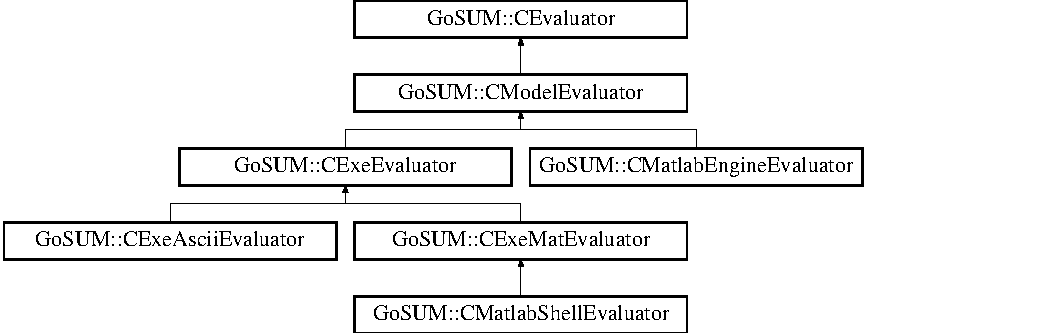
\includegraphics[height=4.465710cm]{class_go_s_u_m_1_1_c_model_evaluator}
\end{center}
\end{figure}
\subsection*{Public Member Functions}
\begin{DoxyCompactItemize}
\item 
\hyperlink{class_go_s_u_m_1_1_c_model_evaluator_a3ba3293fe60b39397a0237b5f8cc78d1}{C\-Model\-Evaluator} ()
\item 
\hyperlink{class_go_s_u_m_1_1_c_model_evaluator_a1cc75e7c7ce09722eb767b1aa1fa1361}{C\-Model\-Evaluator} (const \hyperlink{class_go_s_u_m_1_1_c_input_parameters}{C\-Input\-Parameters} $\ast$\-\_\-p\-I\-P, \hyperlink{class_go_s_u_m_1_1_c_output_states}{C\-Output\-States} $\ast$\-\_\-p\-O\-S, int \-\_\-trd\-I)
\item 
virtual \hyperlink{class_go_s_u_m_1_1_c_model_evaluator_a36f48644d3ab77437fa77acb4418a326}{$\sim$\-C\-Model\-Evaluator} ()
\item 
virtual void \hyperlink{class_go_s_u_m_1_1_c_model_evaluator_a0f5afddb7ed75aad687d3a00e44012a0}{open\-Evaluation} ()=0
\begin{DoxyCompactList}\small\item\em Opens, i.\-e. prepares evaluation process. \end{DoxyCompactList}\item 
virtual Array\-Xd \hyperlink{class_go_s_u_m_1_1_c_model_evaluator_a17541eada67797802edcae14533361ad}{operator()} (const Array\-Xd \&X)=0
\begin{DoxyCompactList}\small\item\em Returns output state evaluated on a single input parameter n-\/tuple. \end{DoxyCompactList}\item 
virtual void \hyperlink{class_go_s_u_m_1_1_c_model_evaluator_a27d4b3c17958df42dd62b0d7d2e064d1}{operator()} ()
\begin{DoxyCompactList}\small\item\em Thread calls this operator which then evalutes output states from every trd\-I-\/th input parameter n-\/tuple. \end{DoxyCompactList}\item 
virtual int \hyperlink{class_go_s_u_m_1_1_c_model_evaluator_a822314faa443612c8840e6252018efb2}{evaluate\-Outputs\-Size} ()
\begin{DoxyCompactList}\small\item\em Evaluates outputs size by running model evaluator. \end{DoxyCompactList}\item 
virtual void \hyperlink{class_go_s_u_m_1_1_c_model_evaluator_a7ed9761e18560616881ebe459c6b8952}{close\-Evaluation} ()=0
\begin{DoxyCompactList}\small\item\em Closes evaluation process. \end{DoxyCompactList}\end{DoxyCompactItemize}
\subsection*{Protected Member Functions}
\begin{DoxyCompactItemize}
\item 
{\footnotesize template$<$class Archive $>$ }\\void \hyperlink{class_go_s_u_m_1_1_c_model_evaluator_a80e334f1496f3bee1da84cee050a72a1}{serialize} (Archive \&ar, const unsigned int version)
\end{DoxyCompactItemize}
\subsection*{Protected Attributes}
\begin{DoxyCompactItemize}
\item 
const \hyperlink{class_go_s_u_m_1_1_c_input_parameters}{C\-Input\-Parameters} $\ast$ \hyperlink{class_go_s_u_m_1_1_c_model_evaluator_a1d6e69bc264c99eda155fe72915fbc8b}{p\-I\-P}
\begin{DoxyCompactList}\small\item\em Pointer to \hyperlink{struct_go_s_u_m}{Go\-S\-U\-M} input parameters. \end{DoxyCompactList}\item 
\hyperlink{class_go_s_u_m_1_1_c_output_states}{C\-Output\-States} $\ast$ \hyperlink{class_go_s_u_m_1_1_c_model_evaluator_a3acd5d24b64c3fbc6b73dad5ea5b9f43}{p\-O\-S}
\begin{DoxyCompactList}\small\item\em Pointer to \hyperlink{struct_go_s_u_m}{Go\-S\-U\-M} output states. \end{DoxyCompactList}\item 
int \hyperlink{class_go_s_u_m_1_1_c_model_evaluator_a3c67f2a94d451003729e0334746637df}{trd\-I}
\item 
int \hyperlink{class_go_s_u_m_1_1_c_model_evaluator_a1098859defc90ea05ba7223b951d4d3b}{I}
\end{DoxyCompactItemize}
\subsection*{Friends}
\begin{DoxyCompactItemize}
\item 
class \hyperlink{class_go_s_u_m_1_1_c_model_evaluator_ac98d07dd8f7b70e16ccb9a01abf56b9c}{boost\-::serialization\-::access}
\begin{DoxyCompactList}\small\item\em Boost serialization. \end{DoxyCompactList}\end{DoxyCompactItemize}
\subsection*{Additional Inherited Members}


\subsection{Detailed Description}
Class for \hyperlink{struct_go_s_u_m}{Go\-S\-U\-M} model evaluator. 

\subsection{Constructor \& Destructor Documentation}
\hypertarget{class_go_s_u_m_1_1_c_model_evaluator_a3ba3293fe60b39397a0237b5f8cc78d1}{\index{Go\-S\-U\-M\-::\-C\-Model\-Evaluator@{Go\-S\-U\-M\-::\-C\-Model\-Evaluator}!C\-Model\-Evaluator@{C\-Model\-Evaluator}}
\index{C\-Model\-Evaluator@{C\-Model\-Evaluator}!GoSUM::CModelEvaluator@{Go\-S\-U\-M\-::\-C\-Model\-Evaluator}}
\subsubsection[{C\-Model\-Evaluator}]{\setlength{\rightskip}{0pt plus 5cm}Go\-S\-U\-M\-::\-C\-Model\-Evaluator\-::\-C\-Model\-Evaluator (
\begin{DoxyParamCaption}
{}
\end{DoxyParamCaption}
)\hspace{0.3cm}{\ttfamily [inline]}}}\label{class_go_s_u_m_1_1_c_model_evaluator_a3ba3293fe60b39397a0237b5f8cc78d1}
\hypertarget{class_go_s_u_m_1_1_c_model_evaluator_a1cc75e7c7ce09722eb767b1aa1fa1361}{\index{Go\-S\-U\-M\-::\-C\-Model\-Evaluator@{Go\-S\-U\-M\-::\-C\-Model\-Evaluator}!C\-Model\-Evaluator@{C\-Model\-Evaluator}}
\index{C\-Model\-Evaluator@{C\-Model\-Evaluator}!GoSUM::CModelEvaluator@{Go\-S\-U\-M\-::\-C\-Model\-Evaluator}}
\subsubsection[{C\-Model\-Evaluator}]{\setlength{\rightskip}{0pt plus 5cm}Go\-S\-U\-M\-::\-C\-Model\-Evaluator\-::\-C\-Model\-Evaluator (
\begin{DoxyParamCaption}
\item[{const {\bf C\-Input\-Parameters} $\ast$}]{\-\_\-p\-I\-P, }
\item[{{\bf C\-Output\-States} $\ast$}]{\-\_\-p\-O\-S, }
\item[{int}]{\-\_\-trd\-I}
\end{DoxyParamCaption}
)\hspace{0.3cm}{\ttfamily [inline]}}}\label{class_go_s_u_m_1_1_c_model_evaluator_a1cc75e7c7ce09722eb767b1aa1fa1361}
\hypertarget{class_go_s_u_m_1_1_c_model_evaluator_a36f48644d3ab77437fa77acb4418a326}{\index{Go\-S\-U\-M\-::\-C\-Model\-Evaluator@{Go\-S\-U\-M\-::\-C\-Model\-Evaluator}!$\sim$\-C\-Model\-Evaluator@{$\sim$\-C\-Model\-Evaluator}}
\index{$\sim$\-C\-Model\-Evaluator@{$\sim$\-C\-Model\-Evaluator}!GoSUM::CModelEvaluator@{Go\-S\-U\-M\-::\-C\-Model\-Evaluator}}
\subsubsection[{$\sim$\-C\-Model\-Evaluator}]{\setlength{\rightskip}{0pt plus 5cm}virtual Go\-S\-U\-M\-::\-C\-Model\-Evaluator\-::$\sim$\-C\-Model\-Evaluator (
\begin{DoxyParamCaption}
{}
\end{DoxyParamCaption}
)\hspace{0.3cm}{\ttfamily [inline]}, {\ttfamily [virtual]}}}\label{class_go_s_u_m_1_1_c_model_evaluator_a36f48644d3ab77437fa77acb4418a326}


\subsection{Member Function Documentation}
\hypertarget{class_go_s_u_m_1_1_c_model_evaluator_a7ed9761e18560616881ebe459c6b8952}{\index{Go\-S\-U\-M\-::\-C\-Model\-Evaluator@{Go\-S\-U\-M\-::\-C\-Model\-Evaluator}!close\-Evaluation@{close\-Evaluation}}
\index{close\-Evaluation@{close\-Evaluation}!GoSUM::CModelEvaluator@{Go\-S\-U\-M\-::\-C\-Model\-Evaluator}}
\subsubsection[{close\-Evaluation}]{\setlength{\rightskip}{0pt plus 5cm}virtual void Go\-S\-U\-M\-::\-C\-Model\-Evaluator\-::close\-Evaluation (
\begin{DoxyParamCaption}
{}
\end{DoxyParamCaption}
)\hspace{0.3cm}{\ttfamily [pure virtual]}}}\label{class_go_s_u_m_1_1_c_model_evaluator_a7ed9761e18560616881ebe459c6b8952}


Closes evaluation process. 



Implemented in \hyperlink{class_go_s_u_m_1_1_c_matlab_engine_evaluator_a238f3a03165e37f5707611ae1e1a53ae}{Go\-S\-U\-M\-::\-C\-Matlab\-Engine\-Evaluator}, and \hyperlink{class_go_s_u_m_1_1_c_exe_evaluator_a0e18062b8ec197437febdfa46dd7b45b}{Go\-S\-U\-M\-::\-C\-Exe\-Evaluator}.

\hypertarget{class_go_s_u_m_1_1_c_model_evaluator_a822314faa443612c8840e6252018efb2}{\index{Go\-S\-U\-M\-::\-C\-Model\-Evaluator@{Go\-S\-U\-M\-::\-C\-Model\-Evaluator}!evaluate\-Outputs\-Size@{evaluate\-Outputs\-Size}}
\index{evaluate\-Outputs\-Size@{evaluate\-Outputs\-Size}!GoSUM::CModelEvaluator@{Go\-S\-U\-M\-::\-C\-Model\-Evaluator}}
\subsubsection[{evaluate\-Outputs\-Size}]{\setlength{\rightskip}{0pt plus 5cm}virtual int Go\-S\-U\-M\-::\-C\-Model\-Evaluator\-::evaluate\-Outputs\-Size (
\begin{DoxyParamCaption}
{}
\end{DoxyParamCaption}
)\hspace{0.3cm}{\ttfamily [inline]}, {\ttfamily [virtual]}}}\label{class_go_s_u_m_1_1_c_model_evaluator_a822314faa443612c8840e6252018efb2}


Evaluates outputs size by running model evaluator. 



Reimplemented in \hyperlink{class_go_s_u_m_1_1_c_matlab_engine_evaluator_a646d7c6412cf8256a65271af5b1aad89}{Go\-S\-U\-M\-::\-C\-Matlab\-Engine\-Evaluator}, and \hyperlink{class_go_s_u_m_1_1_c_exe_evaluator_a3a8ea5f4af5c653421f27ace8fb57181}{Go\-S\-U\-M\-::\-C\-Exe\-Evaluator}.

\hypertarget{class_go_s_u_m_1_1_c_model_evaluator_a0f5afddb7ed75aad687d3a00e44012a0}{\index{Go\-S\-U\-M\-::\-C\-Model\-Evaluator@{Go\-S\-U\-M\-::\-C\-Model\-Evaluator}!open\-Evaluation@{open\-Evaluation}}
\index{open\-Evaluation@{open\-Evaluation}!GoSUM::CModelEvaluator@{Go\-S\-U\-M\-::\-C\-Model\-Evaluator}}
\subsubsection[{open\-Evaluation}]{\setlength{\rightskip}{0pt plus 5cm}virtual void Go\-S\-U\-M\-::\-C\-Model\-Evaluator\-::open\-Evaluation (
\begin{DoxyParamCaption}
{}
\end{DoxyParamCaption}
)\hspace{0.3cm}{\ttfamily [pure virtual]}}}\label{class_go_s_u_m_1_1_c_model_evaluator_a0f5afddb7ed75aad687d3a00e44012a0}


Opens, i.\-e. prepares evaluation process. 



Implemented in \hyperlink{class_go_s_u_m_1_1_c_matlab_engine_evaluator_a878e5b84a93c808806cad12019372722}{Go\-S\-U\-M\-::\-C\-Matlab\-Engine\-Evaluator}, and \hyperlink{class_go_s_u_m_1_1_c_exe_evaluator_abdc5b11c31ed73a34499e135eab45ef8}{Go\-S\-U\-M\-::\-C\-Exe\-Evaluator}.

\hypertarget{class_go_s_u_m_1_1_c_model_evaluator_a17541eada67797802edcae14533361ad}{\index{Go\-S\-U\-M\-::\-C\-Model\-Evaluator@{Go\-S\-U\-M\-::\-C\-Model\-Evaluator}!operator()@{operator()}}
\index{operator()@{operator()}!GoSUM::CModelEvaluator@{Go\-S\-U\-M\-::\-C\-Model\-Evaluator}}
\subsubsection[{operator()}]{\setlength{\rightskip}{0pt plus 5cm}virtual Array\-Xd Go\-S\-U\-M\-::\-C\-Model\-Evaluator\-::operator() (
\begin{DoxyParamCaption}
\item[{const Array\-Xd \&}]{X}
\end{DoxyParamCaption}
)\hspace{0.3cm}{\ttfamily [pure virtual]}}}\label{class_go_s_u_m_1_1_c_model_evaluator_a17541eada67797802edcae14533361ad}


Returns output state evaluated on a single input parameter n-\/tuple. 



Implemented in \hyperlink{class_go_s_u_m_1_1_c_matlab_engine_evaluator_a68cf94eec612bdd72fd032f5631aad66}{Go\-S\-U\-M\-::\-C\-Matlab\-Engine\-Evaluator}, and \hyperlink{class_go_s_u_m_1_1_c_exe_evaluator_ae388d8a8bef01f0a3fc3e6cecb341576}{Go\-S\-U\-M\-::\-C\-Exe\-Evaluator}.

\hypertarget{class_go_s_u_m_1_1_c_model_evaluator_a27d4b3c17958df42dd62b0d7d2e064d1}{\index{Go\-S\-U\-M\-::\-C\-Model\-Evaluator@{Go\-S\-U\-M\-::\-C\-Model\-Evaluator}!operator()@{operator()}}
\index{operator()@{operator()}!GoSUM::CModelEvaluator@{Go\-S\-U\-M\-::\-C\-Model\-Evaluator}}
\subsubsection[{operator()}]{\setlength{\rightskip}{0pt plus 5cm}void Go\-S\-U\-M\-::\-C\-Model\-Evaluator\-::operator() (
\begin{DoxyParamCaption}
{}
\end{DoxyParamCaption}
)\hspace{0.3cm}{\ttfamily [virtual]}}}\label{class_go_s_u_m_1_1_c_model_evaluator_a27d4b3c17958df42dd62b0d7d2e064d1}


Thread calls this operator which then evalutes output states from every trd\-I-\/th input parameter n-\/tuple. 

\hypertarget{class_go_s_u_m_1_1_c_model_evaluator_a80e334f1496f3bee1da84cee050a72a1}{\index{Go\-S\-U\-M\-::\-C\-Model\-Evaluator@{Go\-S\-U\-M\-::\-C\-Model\-Evaluator}!serialize@{serialize}}
\index{serialize@{serialize}!GoSUM::CModelEvaluator@{Go\-S\-U\-M\-::\-C\-Model\-Evaluator}}
\subsubsection[{serialize}]{\setlength{\rightskip}{0pt plus 5cm}template$<$class Archive $>$ void Go\-S\-U\-M\-::\-C\-Model\-Evaluator\-::serialize (
\begin{DoxyParamCaption}
\item[{Archive \&}]{ar, }
\item[{const unsigned int}]{version}
\end{DoxyParamCaption}
)\hspace{0.3cm}{\ttfamily [protected]}}}\label{class_go_s_u_m_1_1_c_model_evaluator_a80e334f1496f3bee1da84cee050a72a1}


Reimplemented from \hyperlink{class_go_s_u_m_1_1_c_evaluator_a4b1d1f83a5a9280b7cbaf65adcc2f7df}{Go\-S\-U\-M\-::\-C\-Evaluator}.



Reimplemented in \hyperlink{class_go_s_u_m_1_1_c_matlab_engine_evaluator_ad33ed3b3581e5da2f7575c0e3f1d9e55}{Go\-S\-U\-M\-::\-C\-Matlab\-Engine\-Evaluator}, \hyperlink{class_go_s_u_m_1_1_c_matlab_shell_evaluator_af84e659441da0694bff64c2d955831b9}{Go\-S\-U\-M\-::\-C\-Matlab\-Shell\-Evaluator}, \hyperlink{class_go_s_u_m_1_1_c_exe_mat_evaluator_a2e5121b751aaeb6f5c805cfe0312c20d}{Go\-S\-U\-M\-::\-C\-Exe\-Mat\-Evaluator}, \hyperlink{class_go_s_u_m_1_1_c_exe_ascii_evaluator_a68297034ace4c45caa7a1dcd5ff022de}{Go\-S\-U\-M\-::\-C\-Exe\-Ascii\-Evaluator}, and \hyperlink{class_go_s_u_m_1_1_c_exe_evaluator_adccb3c9acae9f916d8be1a9720d5bcc1}{Go\-S\-U\-M\-::\-C\-Exe\-Evaluator}.



\subsection{Friends And Related Function Documentation}
\hypertarget{class_go_s_u_m_1_1_c_model_evaluator_ac98d07dd8f7b70e16ccb9a01abf56b9c}{\index{Go\-S\-U\-M\-::\-C\-Model\-Evaluator@{Go\-S\-U\-M\-::\-C\-Model\-Evaluator}!boost\-::serialization\-::access@{boost\-::serialization\-::access}}
\index{boost\-::serialization\-::access@{boost\-::serialization\-::access}!GoSUM::CModelEvaluator@{Go\-S\-U\-M\-::\-C\-Model\-Evaluator}}
\subsubsection[{boost\-::serialization\-::access}]{\setlength{\rightskip}{0pt plus 5cm}friend class boost\-::serialization\-::access\hspace{0.3cm}{\ttfamily [friend]}}}\label{class_go_s_u_m_1_1_c_model_evaluator_ac98d07dd8f7b70e16ccb9a01abf56b9c}


Boost serialization. 



\subsection{Member Data Documentation}
\hypertarget{class_go_s_u_m_1_1_c_model_evaluator_a1098859defc90ea05ba7223b951d4d3b}{\index{Go\-S\-U\-M\-::\-C\-Model\-Evaluator@{Go\-S\-U\-M\-::\-C\-Model\-Evaluator}!I@{I}}
\index{I@{I}!GoSUM::CModelEvaluator@{Go\-S\-U\-M\-::\-C\-Model\-Evaluator}}
\subsubsection[{I}]{\setlength{\rightskip}{0pt plus 5cm}int Go\-S\-U\-M\-::\-C\-Model\-Evaluator\-::\-I\hspace{0.3cm}{\ttfamily [protected]}}}\label{class_go_s_u_m_1_1_c_model_evaluator_a1098859defc90ea05ba7223b951d4d3b}
Total number of threads and id of the particular thread this class runs in. \hypertarget{class_go_s_u_m_1_1_c_model_evaluator_a1d6e69bc264c99eda155fe72915fbc8b}{\index{Go\-S\-U\-M\-::\-C\-Model\-Evaluator@{Go\-S\-U\-M\-::\-C\-Model\-Evaluator}!p\-I\-P@{p\-I\-P}}
\index{p\-I\-P@{p\-I\-P}!GoSUM::CModelEvaluator@{Go\-S\-U\-M\-::\-C\-Model\-Evaluator}}
\subsubsection[{p\-I\-P}]{\setlength{\rightskip}{0pt plus 5cm}const {\bf C\-Input\-Parameters}$\ast$ Go\-S\-U\-M\-::\-C\-Model\-Evaluator\-::p\-I\-P\hspace{0.3cm}{\ttfamily [protected]}}}\label{class_go_s_u_m_1_1_c_model_evaluator_a1d6e69bc264c99eda155fe72915fbc8b}


Pointer to \hyperlink{struct_go_s_u_m}{Go\-S\-U\-M} input parameters. 

\hypertarget{class_go_s_u_m_1_1_c_model_evaluator_a3acd5d24b64c3fbc6b73dad5ea5b9f43}{\index{Go\-S\-U\-M\-::\-C\-Model\-Evaluator@{Go\-S\-U\-M\-::\-C\-Model\-Evaluator}!p\-O\-S@{p\-O\-S}}
\index{p\-O\-S@{p\-O\-S}!GoSUM::CModelEvaluator@{Go\-S\-U\-M\-::\-C\-Model\-Evaluator}}
\subsubsection[{p\-O\-S}]{\setlength{\rightskip}{0pt plus 5cm}{\bf C\-Output\-States}$\ast$ Go\-S\-U\-M\-::\-C\-Model\-Evaluator\-::p\-O\-S\hspace{0.3cm}{\ttfamily [protected]}}}\label{class_go_s_u_m_1_1_c_model_evaluator_a3acd5d24b64c3fbc6b73dad5ea5b9f43}


Pointer to \hyperlink{struct_go_s_u_m}{Go\-S\-U\-M} output states. 

\hypertarget{class_go_s_u_m_1_1_c_model_evaluator_a3c67f2a94d451003729e0334746637df}{\index{Go\-S\-U\-M\-::\-C\-Model\-Evaluator@{Go\-S\-U\-M\-::\-C\-Model\-Evaluator}!trd\-I@{trd\-I}}
\index{trd\-I@{trd\-I}!GoSUM::CModelEvaluator@{Go\-S\-U\-M\-::\-C\-Model\-Evaluator}}
\subsubsection[{trd\-I}]{\setlength{\rightskip}{0pt plus 5cm}int Go\-S\-U\-M\-::\-C\-Model\-Evaluator\-::trd\-I\hspace{0.3cm}{\ttfamily [protected]}}}\label{class_go_s_u_m_1_1_c_model_evaluator_a3c67f2a94d451003729e0334746637df}


The documentation for this class was generated from the following files\-:\begin{DoxyCompactItemize}
\item 
C\-:/\-Development/core/\hyperlink{_original_model_8h}{Original\-Model.\-h}\item 
C\-:/\-Development/core/\hyperlink{_original_model_8cpp}{Original\-Model.\-cpp}\end{DoxyCompactItemize}

\hypertarget{class_go_s_u_m_1_1_c_model_hypercube}{\section{Go\-S\-U\-M\-:\-:C\-Model\-Hypercube Class Reference}
\label{class_go_s_u_m_1_1_c_model_hypercube}\index{Go\-S\-U\-M\-::\-C\-Model\-Hypercube@{Go\-S\-U\-M\-::\-C\-Model\-Hypercube}}
}


{\ttfamily \#include $<$Hypercube.\-h$>$}

Inheritance diagram for Go\-S\-U\-M\-:\-:C\-Model\-Hypercube\-:\begin{figure}[H]
\begin{center}
\leavevmode
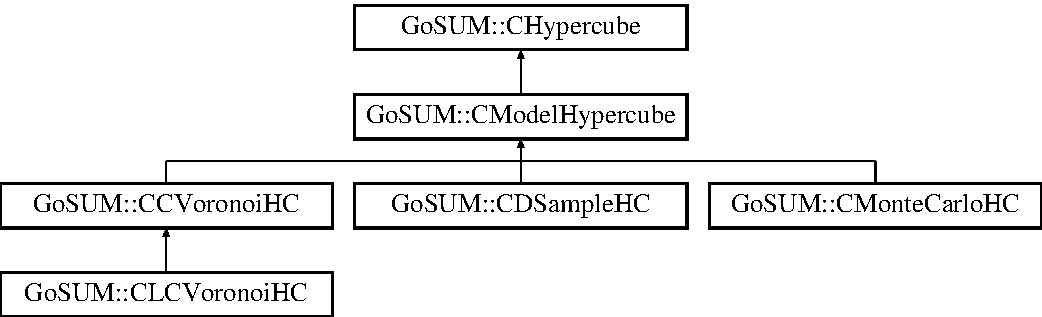
\includegraphics[height=4.000000cm]{class_go_s_u_m_1_1_c_model_hypercube}
\end{center}
\end{figure}
\subsection*{Public Member Functions}
\begin{DoxyCompactItemize}
\item 
\hyperlink{class_go_s_u_m_1_1_c_model_hypercube_ab16030ca1067a265077a762fb56caf46}{C\-Model\-Hypercube} (\hyperlink{class_go_s_u_m_1_1_c_input_parameters}{C\-Input\-Parameters} $\ast$\-\_\-p\-I\-P)
\item 
virtual \hyperlink{class_go_s_u_m_1_1_c_model_hypercube_aa7ab99f4bad3c65123675a2d29c7cf87}{$\sim$\-C\-Model\-Hypercube} ()
\item 
virtual void \hyperlink{class_go_s_u_m_1_1_c_model_hypercube_acd201b7a6dcab576a907f85c127fa6ce}{generate} (int \-\_\-rssize, int \-\_\-dim, std\-::vector$<$ Array\-Xd $>$ \&\-\_\-samples)
\begin{DoxyCompactList}\small\item\em Generates \-\_\-samples\-: \-\_\-rssize model points (satisifing constraints) of dimension \-\_\-dim. \end{DoxyCompactList}\end{DoxyCompactItemize}
\subsection*{Protected Member Functions}
\begin{DoxyCompactItemize}
\item 
{\footnotesize template$<$class Archive $>$ }\\void \hyperlink{class_go_s_u_m_1_1_c_model_hypercube_a67de6632c6f6ca3685d2a750599974c6}{serialize} (Archive \&ar, const unsigned int version)
\item 
Array\-Xd \& \hyperlink{class_go_s_u_m_1_1_c_model_hypercube_a4d64e5c09e2ed5a270ac67d44635c07c}{generate\-H\-C\-Point} (Array\-Xd \&x)
\item 
void \hyperlink{class_go_s_u_m_1_1_c_model_hypercube_ae52705f007701d127b797845f4c2ad6b}{generate\-H\-C\-Points} (int N, int dim, std\-::vector$<$ Array\-Xd $>$ \&y)
\begin{DoxyCompactList}\small\item\em Generates N hypercube points. \end{DoxyCompactList}\item 
void \hyperlink{class_go_s_u_m_1_1_c_model_hypercube_a2b5a2350b562bbb6d130e7791d5bb5e4}{generate\-Model\-Points} (int N, int dim, std\-::vector$<$ Array\-Xd $>$ \&y)
\begin{DoxyCompactList}\small\item\em Generates N model points. \end{DoxyCompactList}\item 
void \hyperlink{class_go_s_u_m_1_1_c_model_hypercube_a1419c038ee212ec1bc80420da32a7351}{check\-H\-C\-Points} (std\-::vector$<$ Array\-Xd $>$ \&y)
\begin{DoxyCompactList}\small\item\em Checks if hypercube points when mapped to model points satisfy constraints. \end{DoxyCompactList}\item 
void \hyperlink{class_go_s_u_m_1_1_c_model_hypercube_adcf1da087b48ec609994853abae9c52e}{hc\-Points2\-Model\-Points} (std\-::vector$<$ Array\-Xd $>$ \&y)
\begin{DoxyCompactList}\small\item\em Maps hypercube points to model points. \end{DoxyCompactList}\item 
virtual void \hyperlink{class_go_s_u_m_1_1_c_model_hypercube_a1e92dd784f1c20b604fecd1a48bea2f4}{do\-Generate} (int \-\_\-rssize, int \-\_\-dim, std\-::vector$<$ Array\-Xd $>$ \&\-\_\-samples)=0
\begin{DoxyCompactList}\small\item\em Core of the generation. \end{DoxyCompactList}\item 
\hyperlink{class_go_s_u_m_1_1_c_model_hypercube_a2bd3061ba2c197b831389341a0ff5661}{C\-Model\-Hypercube} ()
\end{DoxyCompactItemize}
\subsection*{Protected Attributes}
\begin{DoxyCompactItemize}
\item 
\hyperlink{class_go_s_u_m_1_1_c_input_parameters}{C\-Input\-Parameters} $\ast$ \hyperlink{class_go_s_u_m_1_1_c_model_hypercube_a7382643c37cf27c4b1e881bdf08b7ff4}{p\-I\-P}
\begin{DoxyCompactList}\small\item\em Holds pointer to input parameters. \end{DoxyCompactList}\item 
\hyperlink{class_go_s_u_m_1_1_c_model_constraints}{C\-Model\-Constraints} $\ast$ \hyperlink{class_go_s_u_m_1_1_c_model_hypercube_afefc6601f2bb4b95c7bd56250fcef2c4}{p\-I\-C}
\begin{DoxyCompactList}\small\item\em Holds pointer to input parameter constraints. \end{DoxyCompactList}\item 
int \hyperlink{class_go_s_u_m_1_1_c_model_hypercube_a2b0d3bcbf328d89f7bcb3706795dbbc4}{maxtries}
\end{DoxyCompactItemize}
\subsection*{Friends}
\begin{DoxyCompactItemize}
\item 
class \hyperlink{class_go_s_u_m_1_1_c_model_hypercube_ac98d07dd8f7b70e16ccb9a01abf56b9c}{boost\-::serialization\-::access}
\begin{DoxyCompactList}\small\item\em Boost serialization. \end{DoxyCompactList}\end{DoxyCompactItemize}
\subsection*{Additional Inherited Members}


\subsection{Constructor \& Destructor Documentation}
\hypertarget{class_go_s_u_m_1_1_c_model_hypercube_a2bd3061ba2c197b831389341a0ff5661}{\index{Go\-S\-U\-M\-::\-C\-Model\-Hypercube@{Go\-S\-U\-M\-::\-C\-Model\-Hypercube}!C\-Model\-Hypercube@{C\-Model\-Hypercube}}
\index{C\-Model\-Hypercube@{C\-Model\-Hypercube}!GoSUM::CModelHypercube@{Go\-S\-U\-M\-::\-C\-Model\-Hypercube}}
\subsubsection[{C\-Model\-Hypercube}]{\setlength{\rightskip}{0pt plus 5cm}Go\-S\-U\-M\-::\-C\-Model\-Hypercube\-::\-C\-Model\-Hypercube (
\begin{DoxyParamCaption}
{}
\end{DoxyParamCaption}
)\hspace{0.3cm}{\ttfamily [inline]}, {\ttfamily [protected]}}}\label{class_go_s_u_m_1_1_c_model_hypercube_a2bd3061ba2c197b831389341a0ff5661}
\hypertarget{class_go_s_u_m_1_1_c_model_hypercube_ab16030ca1067a265077a762fb56caf46}{\index{Go\-S\-U\-M\-::\-C\-Model\-Hypercube@{Go\-S\-U\-M\-::\-C\-Model\-Hypercube}!C\-Model\-Hypercube@{C\-Model\-Hypercube}}
\index{C\-Model\-Hypercube@{C\-Model\-Hypercube}!GoSUM::CModelHypercube@{Go\-S\-U\-M\-::\-C\-Model\-Hypercube}}
\subsubsection[{C\-Model\-Hypercube}]{\setlength{\rightskip}{0pt plus 5cm}Go\-S\-U\-M\-::\-C\-Model\-Hypercube\-::\-C\-Model\-Hypercube (
\begin{DoxyParamCaption}
\item[{{\bf C\-Input\-Parameters} $\ast$}]{\-\_\-p\-I\-P}
\end{DoxyParamCaption}
)\hspace{0.3cm}{\ttfamily [inline]}}}\label{class_go_s_u_m_1_1_c_model_hypercube_ab16030ca1067a265077a762fb56caf46}
\hypertarget{class_go_s_u_m_1_1_c_model_hypercube_aa7ab99f4bad3c65123675a2d29c7cf87}{\index{Go\-S\-U\-M\-::\-C\-Model\-Hypercube@{Go\-S\-U\-M\-::\-C\-Model\-Hypercube}!$\sim$\-C\-Model\-Hypercube@{$\sim$\-C\-Model\-Hypercube}}
\index{$\sim$\-C\-Model\-Hypercube@{$\sim$\-C\-Model\-Hypercube}!GoSUM::CModelHypercube@{Go\-S\-U\-M\-::\-C\-Model\-Hypercube}}
\subsubsection[{$\sim$\-C\-Model\-Hypercube}]{\setlength{\rightskip}{0pt plus 5cm}virtual Go\-S\-U\-M\-::\-C\-Model\-Hypercube\-::$\sim$\-C\-Model\-Hypercube (
\begin{DoxyParamCaption}
{}
\end{DoxyParamCaption}
)\hspace{0.3cm}{\ttfamily [inline]}, {\ttfamily [virtual]}}}\label{class_go_s_u_m_1_1_c_model_hypercube_aa7ab99f4bad3c65123675a2d29c7cf87}


\subsection{Member Function Documentation}
\hypertarget{class_go_s_u_m_1_1_c_model_hypercube_a1419c038ee212ec1bc80420da32a7351}{\index{Go\-S\-U\-M\-::\-C\-Model\-Hypercube@{Go\-S\-U\-M\-::\-C\-Model\-Hypercube}!check\-H\-C\-Points@{check\-H\-C\-Points}}
\index{check\-H\-C\-Points@{check\-H\-C\-Points}!GoSUM::CModelHypercube@{Go\-S\-U\-M\-::\-C\-Model\-Hypercube}}
\subsubsection[{check\-H\-C\-Points}]{\setlength{\rightskip}{0pt plus 5cm}void Go\-S\-U\-M\-::\-C\-Model\-Hypercube\-::check\-H\-C\-Points (
\begin{DoxyParamCaption}
\item[{std\-::vector$<$ Array\-Xd $>$ \&}]{y}
\end{DoxyParamCaption}
)\hspace{0.3cm}{\ttfamily [protected]}}}\label{class_go_s_u_m_1_1_c_model_hypercube_a1419c038ee212ec1bc80420da32a7351}


Checks if hypercube points when mapped to model points satisfy constraints. 

\hypertarget{class_go_s_u_m_1_1_c_model_hypercube_a1e92dd784f1c20b604fecd1a48bea2f4}{\index{Go\-S\-U\-M\-::\-C\-Model\-Hypercube@{Go\-S\-U\-M\-::\-C\-Model\-Hypercube}!do\-Generate@{do\-Generate}}
\index{do\-Generate@{do\-Generate}!GoSUM::CModelHypercube@{Go\-S\-U\-M\-::\-C\-Model\-Hypercube}}
\subsubsection[{do\-Generate}]{\setlength{\rightskip}{0pt plus 5cm}virtual void Go\-S\-U\-M\-::\-C\-Model\-Hypercube\-::do\-Generate (
\begin{DoxyParamCaption}
\item[{int}]{\-\_\-rssize, }
\item[{int}]{\-\_\-dim, }
\item[{std\-::vector$<$ Array\-Xd $>$ \&}]{\-\_\-samples}
\end{DoxyParamCaption}
)\hspace{0.3cm}{\ttfamily [protected]}, {\ttfamily [pure virtual]}}}\label{class_go_s_u_m_1_1_c_model_hypercube_a1e92dd784f1c20b604fecd1a48bea2f4}


Core of the generation. 



Implemented in \hyperlink{class_go_s_u_m_1_1_c_l_c_voronoi_h_c_a02e90ea8deecafc3b398709f748fa9af}{Go\-S\-U\-M\-::\-C\-L\-C\-Voronoi\-H\-C}, \hyperlink{class_go_s_u_m_1_1_c_c_voronoi_h_c_ae3ecc9c8e8c09e42c13b77d0bfa8c020}{Go\-S\-U\-M\-::\-C\-C\-Voronoi\-H\-C}, \hyperlink{class_go_s_u_m_1_1_c_monte_carlo_h_c_a848c0dded522350b9d6edb41497e19d1}{Go\-S\-U\-M\-::\-C\-Monte\-Carlo\-H\-C}, and \hyperlink{class_go_s_u_m_1_1_c_d_sample_h_c_aaa41eae7d120c7bf8d29ed2a0dc5c470}{Go\-S\-U\-M\-::\-C\-D\-Sample\-H\-C}.

\hypertarget{class_go_s_u_m_1_1_c_model_hypercube_acd201b7a6dcab576a907f85c127fa6ce}{\index{Go\-S\-U\-M\-::\-C\-Model\-Hypercube@{Go\-S\-U\-M\-::\-C\-Model\-Hypercube}!generate@{generate}}
\index{generate@{generate}!GoSUM::CModelHypercube@{Go\-S\-U\-M\-::\-C\-Model\-Hypercube}}
\subsubsection[{generate}]{\setlength{\rightskip}{0pt plus 5cm}void Go\-S\-U\-M\-::\-C\-Model\-Hypercube\-::generate (
\begin{DoxyParamCaption}
\item[{int}]{\-\_\-rssize, }
\item[{int}]{\-\_\-dim, }
\item[{std\-::vector$<$ Array\-Xd $>$ \&}]{\-\_\-samples}
\end{DoxyParamCaption}
)\hspace{0.3cm}{\ttfamily [virtual]}}}\label{class_go_s_u_m_1_1_c_model_hypercube_acd201b7a6dcab576a907f85c127fa6ce}


Generates \-\_\-samples\-: \-\_\-rssize model points (satisifing constraints) of dimension \-\_\-dim. 

\hypertarget{class_go_s_u_m_1_1_c_model_hypercube_a4d64e5c09e2ed5a270ac67d44635c07c}{\index{Go\-S\-U\-M\-::\-C\-Model\-Hypercube@{Go\-S\-U\-M\-::\-C\-Model\-Hypercube}!generate\-H\-C\-Point@{generate\-H\-C\-Point}}
\index{generate\-H\-C\-Point@{generate\-H\-C\-Point}!GoSUM::CModelHypercube@{Go\-S\-U\-M\-::\-C\-Model\-Hypercube}}
\subsubsection[{generate\-H\-C\-Point}]{\setlength{\rightskip}{0pt plus 5cm}Array\-Xd\& Go\-S\-U\-M\-::\-C\-Model\-Hypercube\-::generate\-H\-C\-Point (
\begin{DoxyParamCaption}
\item[{Array\-Xd \&}]{x}
\end{DoxyParamCaption}
)\hspace{0.3cm}{\ttfamily [inline]}, {\ttfamily [protected]}}}\label{class_go_s_u_m_1_1_c_model_hypercube_a4d64e5c09e2ed5a270ac67d44635c07c}

\begin{DoxyParams}{Parameters}
{\em x} & Generates single hypercube point. \\
\hline
\end{DoxyParams}
\hypertarget{class_go_s_u_m_1_1_c_model_hypercube_ae52705f007701d127b797845f4c2ad6b}{\index{Go\-S\-U\-M\-::\-C\-Model\-Hypercube@{Go\-S\-U\-M\-::\-C\-Model\-Hypercube}!generate\-H\-C\-Points@{generate\-H\-C\-Points}}
\index{generate\-H\-C\-Points@{generate\-H\-C\-Points}!GoSUM::CModelHypercube@{Go\-S\-U\-M\-::\-C\-Model\-Hypercube}}
\subsubsection[{generate\-H\-C\-Points}]{\setlength{\rightskip}{0pt plus 5cm}void Go\-S\-U\-M\-::\-C\-Model\-Hypercube\-::generate\-H\-C\-Points (
\begin{DoxyParamCaption}
\item[{int}]{N, }
\item[{int}]{dim, }
\item[{std\-::vector$<$ Array\-Xd $>$ \&}]{y}
\end{DoxyParamCaption}
)\hspace{0.3cm}{\ttfamily [protected]}}}\label{class_go_s_u_m_1_1_c_model_hypercube_ae52705f007701d127b797845f4c2ad6b}


Generates N hypercube points. 

\hypertarget{class_go_s_u_m_1_1_c_model_hypercube_a2b5a2350b562bbb6d130e7791d5bb5e4}{\index{Go\-S\-U\-M\-::\-C\-Model\-Hypercube@{Go\-S\-U\-M\-::\-C\-Model\-Hypercube}!generate\-Model\-Points@{generate\-Model\-Points}}
\index{generate\-Model\-Points@{generate\-Model\-Points}!GoSUM::CModelHypercube@{Go\-S\-U\-M\-::\-C\-Model\-Hypercube}}
\subsubsection[{generate\-Model\-Points}]{\setlength{\rightskip}{0pt plus 5cm}void Go\-S\-U\-M\-::\-C\-Model\-Hypercube\-::generate\-Model\-Points (
\begin{DoxyParamCaption}
\item[{int}]{N, }
\item[{int}]{dim, }
\item[{std\-::vector$<$ Array\-Xd $>$ \&}]{y}
\end{DoxyParamCaption}
)\hspace{0.3cm}{\ttfamily [protected]}}}\label{class_go_s_u_m_1_1_c_model_hypercube_a2b5a2350b562bbb6d130e7791d5bb5e4}


Generates N model points. 

\hypertarget{class_go_s_u_m_1_1_c_model_hypercube_adcf1da087b48ec609994853abae9c52e}{\index{Go\-S\-U\-M\-::\-C\-Model\-Hypercube@{Go\-S\-U\-M\-::\-C\-Model\-Hypercube}!hc\-Points2\-Model\-Points@{hc\-Points2\-Model\-Points}}
\index{hc\-Points2\-Model\-Points@{hc\-Points2\-Model\-Points}!GoSUM::CModelHypercube@{Go\-S\-U\-M\-::\-C\-Model\-Hypercube}}
\subsubsection[{hc\-Points2\-Model\-Points}]{\setlength{\rightskip}{0pt plus 5cm}void Go\-S\-U\-M\-::\-C\-Model\-Hypercube\-::hc\-Points2\-Model\-Points (
\begin{DoxyParamCaption}
\item[{std\-::vector$<$ Array\-Xd $>$ \&}]{y}
\end{DoxyParamCaption}
)\hspace{0.3cm}{\ttfamily [protected]}}}\label{class_go_s_u_m_1_1_c_model_hypercube_adcf1da087b48ec609994853abae9c52e}


Maps hypercube points to model points. 

\hypertarget{class_go_s_u_m_1_1_c_model_hypercube_a67de6632c6f6ca3685d2a750599974c6}{\index{Go\-S\-U\-M\-::\-C\-Model\-Hypercube@{Go\-S\-U\-M\-::\-C\-Model\-Hypercube}!serialize@{serialize}}
\index{serialize@{serialize}!GoSUM::CModelHypercube@{Go\-S\-U\-M\-::\-C\-Model\-Hypercube}}
\subsubsection[{serialize}]{\setlength{\rightskip}{0pt plus 5cm}template$<$class Archive $>$ void Go\-S\-U\-M\-::\-C\-Model\-Hypercube\-::serialize (
\begin{DoxyParamCaption}
\item[{Archive \&}]{ar, }
\item[{const unsigned int}]{version}
\end{DoxyParamCaption}
)\hspace{0.3cm}{\ttfamily [protected]}}}\label{class_go_s_u_m_1_1_c_model_hypercube_a67de6632c6f6ca3685d2a750599974c6}


Reimplemented from \hyperlink{class_go_s_u_m_1_1_c_hypercube_a7303a209b69f0d628b8d2249867e9247}{Go\-S\-U\-M\-::\-C\-Hypercube}.



Reimplemented in \hyperlink{class_go_s_u_m_1_1_c_l_c_voronoi_h_c_a98f588c33a8f2e2f4b681b48d63f2109}{Go\-S\-U\-M\-::\-C\-L\-C\-Voronoi\-H\-C}, \hyperlink{class_go_s_u_m_1_1_c_c_voronoi_h_c_abbeaabd93028069b81be4dfc078e3d02}{Go\-S\-U\-M\-::\-C\-C\-Voronoi\-H\-C}, and \hyperlink{class_go_s_u_m_1_1_c_monte_carlo_h_c_ae04ab348b02072028893eee2541cadf8}{Go\-S\-U\-M\-::\-C\-Monte\-Carlo\-H\-C}.



\subsection{Friends And Related Function Documentation}
\hypertarget{class_go_s_u_m_1_1_c_model_hypercube_ac98d07dd8f7b70e16ccb9a01abf56b9c}{\index{Go\-S\-U\-M\-::\-C\-Model\-Hypercube@{Go\-S\-U\-M\-::\-C\-Model\-Hypercube}!boost\-::serialization\-::access@{boost\-::serialization\-::access}}
\index{boost\-::serialization\-::access@{boost\-::serialization\-::access}!GoSUM::CModelHypercube@{Go\-S\-U\-M\-::\-C\-Model\-Hypercube}}
\subsubsection[{boost\-::serialization\-::access}]{\setlength{\rightskip}{0pt plus 5cm}friend class boost\-::serialization\-::access\hspace{0.3cm}{\ttfamily [friend]}}}\label{class_go_s_u_m_1_1_c_model_hypercube_ac98d07dd8f7b70e16ccb9a01abf56b9c}


Boost serialization. 



\subsection{Member Data Documentation}
\hypertarget{class_go_s_u_m_1_1_c_model_hypercube_a2b0d3bcbf328d89f7bcb3706795dbbc4}{\index{Go\-S\-U\-M\-::\-C\-Model\-Hypercube@{Go\-S\-U\-M\-::\-C\-Model\-Hypercube}!maxtries@{maxtries}}
\index{maxtries@{maxtries}!GoSUM::CModelHypercube@{Go\-S\-U\-M\-::\-C\-Model\-Hypercube}}
\subsubsection[{maxtries}]{\setlength{\rightskip}{0pt plus 5cm}int Go\-S\-U\-M\-::\-C\-Model\-Hypercube\-::maxtries\hspace{0.3cm}{\ttfamily [protected]}}}\label{class_go_s_u_m_1_1_c_model_hypercube_a2b0d3bcbf328d89f7bcb3706795dbbc4}
Holds maximal number of tries to satisfy model constraints. \hypertarget{class_go_s_u_m_1_1_c_model_hypercube_afefc6601f2bb4b95c7bd56250fcef2c4}{\index{Go\-S\-U\-M\-::\-C\-Model\-Hypercube@{Go\-S\-U\-M\-::\-C\-Model\-Hypercube}!p\-I\-C@{p\-I\-C}}
\index{p\-I\-C@{p\-I\-C}!GoSUM::CModelHypercube@{Go\-S\-U\-M\-::\-C\-Model\-Hypercube}}
\subsubsection[{p\-I\-C}]{\setlength{\rightskip}{0pt plus 5cm}{\bf C\-Model\-Constraints}$\ast$ Go\-S\-U\-M\-::\-C\-Model\-Hypercube\-::p\-I\-C\hspace{0.3cm}{\ttfamily [protected]}}}\label{class_go_s_u_m_1_1_c_model_hypercube_afefc6601f2bb4b95c7bd56250fcef2c4}


Holds pointer to input parameter constraints. 

\hypertarget{class_go_s_u_m_1_1_c_model_hypercube_a7382643c37cf27c4b1e881bdf08b7ff4}{\index{Go\-S\-U\-M\-::\-C\-Model\-Hypercube@{Go\-S\-U\-M\-::\-C\-Model\-Hypercube}!p\-I\-P@{p\-I\-P}}
\index{p\-I\-P@{p\-I\-P}!GoSUM::CModelHypercube@{Go\-S\-U\-M\-::\-C\-Model\-Hypercube}}
\subsubsection[{p\-I\-P}]{\setlength{\rightskip}{0pt plus 5cm}{\bf C\-Input\-Parameters}$\ast$ Go\-S\-U\-M\-::\-C\-Model\-Hypercube\-::p\-I\-P\hspace{0.3cm}{\ttfamily [protected]}}}\label{class_go_s_u_m_1_1_c_model_hypercube_a7382643c37cf27c4b1e881bdf08b7ff4}


Holds pointer to input parameters. 



The documentation for this class was generated from the following files\-:\begin{DoxyCompactItemize}
\item 
C\-:/\-Development/core/\hyperlink{_hypercube_8h}{Hypercube.\-h}\item 
C\-:/\-Development/core/\hyperlink{_hypercube_8cpp}{Hypercube.\-cpp}\end{DoxyCompactItemize}

\hypertarget{class_go_s_u_m_1_1_c_model_optimization_variable}{\section{Go\-S\-U\-M\-:\-:C\-Model\-Optimization\-Variable Class Reference}
\label{class_go_s_u_m_1_1_c_model_optimization_variable}\index{Go\-S\-U\-M\-::\-C\-Model\-Optimization\-Variable@{Go\-S\-U\-M\-::\-C\-Model\-Optimization\-Variable}}
}


{\ttfamily \#include $<$Parser\-Optimization\-Problem.\-h$>$}

Inheritance diagram for Go\-S\-U\-M\-:\-:C\-Model\-Optimization\-Variable\-:\begin{figure}[H]
\begin{center}
\leavevmode
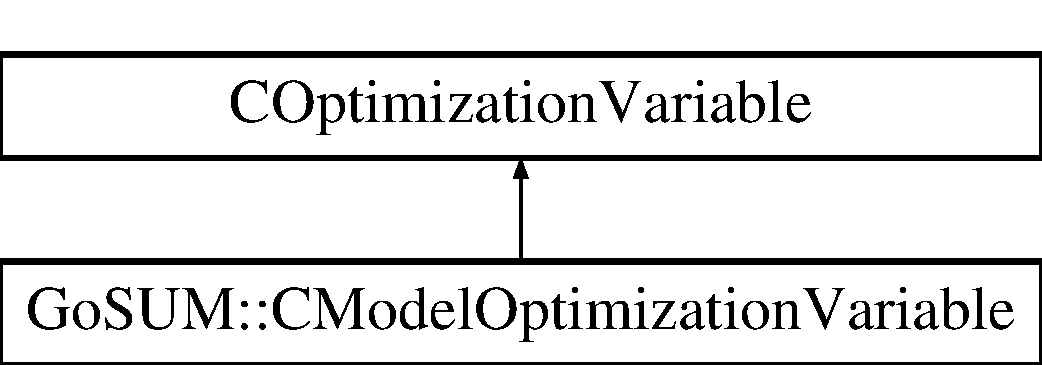
\includegraphics[height=2.000000cm]{class_go_s_u_m_1_1_c_model_optimization_variable}
\end{center}
\end{figure}
\subsection*{Public Member Functions}
\begin{DoxyCompactItemize}
\item 
\hyperlink{class_go_s_u_m_1_1_c_model_optimization_variable_a901bd687dbccbd0dc8d1cad66b1dea74}{C\-Model\-Optimization\-Variable} (\hyperlink{class_go_s_u_m_1_1_c_model_variable}{C\-Model\-Variable} $\ast$\-\_\-pip)
\item 
\hyperlink{class_go_s_u_m_1_1_c_model_optimization_variable_a27afbb2cec03c53c61fe320f2b76fe91}{C\-Model\-Optimization\-Variable} (\hyperlink{class_go_s_u_m_1_1_c_model_optimization_variable}{C\-Model\-Optimization\-Variable} \&\-\_\-\-O)
\item 
virtual \hyperlink{class_go_s_u_m_1_1_c_model_optimization_variable_a7e6ec9d63b330feff1d6820584cb4ff3}{$\sim$\-C\-Model\-Optimization\-Variable} ()
\item 
\hyperlink{class_go_s_u_m_1_1_c_model_variable}{C\-Model\-Variable} $\ast$ \hyperlink{class_go_s_u_m_1_1_c_model_optimization_variable_a4dc3d3f397b418672f3b271a86dfd066}{input\-Parameter} () const 
\begin{DoxyCompactList}\small\item\em Returns pointer to the input parameter to which model optimization variable is connected. \end{DoxyCompactList}\item 
void \hyperlink{class_go_s_u_m_1_1_c_model_optimization_variable_ab3b5c74ba04de1583eba92aa2844ff71}{reset} ()
\begin{DoxyCompactList}\small\item\em Resets lower bound, upper bound and inital value. \end{DoxyCompactList}\end{DoxyCompactItemize}
\subsection*{Protected Member Functions}
\begin{DoxyCompactItemize}
\item 
{\footnotesize template$<$class Archive $>$ }\\void \hyperlink{class_go_s_u_m_1_1_c_model_optimization_variable_ac2e916e3523fec4487a8f567bb0a1af9}{serialize} (Archive \&ar, const unsigned int version)
\item 
\hyperlink{class_go_s_u_m_1_1_c_model_optimization_variable_a815f4d1d5b575f853e1248147bce755b}{C\-Model\-Optimization\-Variable} ()
\end{DoxyCompactItemize}
\subsection*{Protected Attributes}
\begin{DoxyCompactItemize}
\item 
\hyperlink{class_go_s_u_m_1_1_c_model_variable}{C\-Model\-Variable} $\ast$ \hyperlink{class_go_s_u_m_1_1_c_model_optimization_variable_ab1f22680bcb939d871b717126ea555f1}{pip}
\end{DoxyCompactItemize}
\subsection*{Friends}
\begin{DoxyCompactItemize}
\item 
class \hyperlink{class_go_s_u_m_1_1_c_model_optimization_variable_ac98d07dd8f7b70e16ccb9a01abf56b9c}{boost\-::serialization\-::access}
\begin{DoxyCompactList}\small\item\em Boost serialization. \end{DoxyCompactList}\end{DoxyCompactItemize}


\subsection{Constructor \& Destructor Documentation}
\hypertarget{class_go_s_u_m_1_1_c_model_optimization_variable_a815f4d1d5b575f853e1248147bce755b}{\index{Go\-S\-U\-M\-::\-C\-Model\-Optimization\-Variable@{Go\-S\-U\-M\-::\-C\-Model\-Optimization\-Variable}!C\-Model\-Optimization\-Variable@{C\-Model\-Optimization\-Variable}}
\index{C\-Model\-Optimization\-Variable@{C\-Model\-Optimization\-Variable}!GoSUM::CModelOptimizationVariable@{Go\-S\-U\-M\-::\-C\-Model\-Optimization\-Variable}}
\subsubsection[{C\-Model\-Optimization\-Variable}]{\setlength{\rightskip}{0pt plus 5cm}Go\-S\-U\-M\-::\-C\-Model\-Optimization\-Variable\-::\-C\-Model\-Optimization\-Variable (
\begin{DoxyParamCaption}
{}
\end{DoxyParamCaption}
)\hspace{0.3cm}{\ttfamily [inline]}, {\ttfamily [protected]}}}\label{class_go_s_u_m_1_1_c_model_optimization_variable_a815f4d1d5b575f853e1248147bce755b}
\hypertarget{class_go_s_u_m_1_1_c_model_optimization_variable_a901bd687dbccbd0dc8d1cad66b1dea74}{\index{Go\-S\-U\-M\-::\-C\-Model\-Optimization\-Variable@{Go\-S\-U\-M\-::\-C\-Model\-Optimization\-Variable}!C\-Model\-Optimization\-Variable@{C\-Model\-Optimization\-Variable}}
\index{C\-Model\-Optimization\-Variable@{C\-Model\-Optimization\-Variable}!GoSUM::CModelOptimizationVariable@{Go\-S\-U\-M\-::\-C\-Model\-Optimization\-Variable}}
\subsubsection[{C\-Model\-Optimization\-Variable}]{\setlength{\rightskip}{0pt plus 5cm}Go\-S\-U\-M\-::\-C\-Model\-Optimization\-Variable\-::\-C\-Model\-Optimization\-Variable (
\begin{DoxyParamCaption}
\item[{{\bf C\-Model\-Variable} $\ast$}]{\-\_\-pip}
\end{DoxyParamCaption}
)\hspace{0.3cm}{\ttfamily [inline]}}}\label{class_go_s_u_m_1_1_c_model_optimization_variable_a901bd687dbccbd0dc8d1cad66b1dea74}
\hypertarget{class_go_s_u_m_1_1_c_model_optimization_variable_a27afbb2cec03c53c61fe320f2b76fe91}{\index{Go\-S\-U\-M\-::\-C\-Model\-Optimization\-Variable@{Go\-S\-U\-M\-::\-C\-Model\-Optimization\-Variable}!C\-Model\-Optimization\-Variable@{C\-Model\-Optimization\-Variable}}
\index{C\-Model\-Optimization\-Variable@{C\-Model\-Optimization\-Variable}!GoSUM::CModelOptimizationVariable@{Go\-S\-U\-M\-::\-C\-Model\-Optimization\-Variable}}
\subsubsection[{C\-Model\-Optimization\-Variable}]{\setlength{\rightskip}{0pt plus 5cm}Go\-S\-U\-M\-::\-C\-Model\-Optimization\-Variable\-::\-C\-Model\-Optimization\-Variable (
\begin{DoxyParamCaption}
\item[{{\bf C\-Model\-Optimization\-Variable} \&}]{\-\_\-\-O}
\end{DoxyParamCaption}
)\hspace{0.3cm}{\ttfamily [inline]}}}\label{class_go_s_u_m_1_1_c_model_optimization_variable_a27afbb2cec03c53c61fe320f2b76fe91}
\hypertarget{class_go_s_u_m_1_1_c_model_optimization_variable_a7e6ec9d63b330feff1d6820584cb4ff3}{\index{Go\-S\-U\-M\-::\-C\-Model\-Optimization\-Variable@{Go\-S\-U\-M\-::\-C\-Model\-Optimization\-Variable}!$\sim$\-C\-Model\-Optimization\-Variable@{$\sim$\-C\-Model\-Optimization\-Variable}}
\index{$\sim$\-C\-Model\-Optimization\-Variable@{$\sim$\-C\-Model\-Optimization\-Variable}!GoSUM::CModelOptimizationVariable@{Go\-S\-U\-M\-::\-C\-Model\-Optimization\-Variable}}
\subsubsection[{$\sim$\-C\-Model\-Optimization\-Variable}]{\setlength{\rightskip}{0pt plus 5cm}virtual Go\-S\-U\-M\-::\-C\-Model\-Optimization\-Variable\-::$\sim$\-C\-Model\-Optimization\-Variable (
\begin{DoxyParamCaption}
{}
\end{DoxyParamCaption}
)\hspace{0.3cm}{\ttfamily [inline]}, {\ttfamily [virtual]}}}\label{class_go_s_u_m_1_1_c_model_optimization_variable_a7e6ec9d63b330feff1d6820584cb4ff3}


\subsection{Member Function Documentation}
\hypertarget{class_go_s_u_m_1_1_c_model_optimization_variable_a4dc3d3f397b418672f3b271a86dfd066}{\index{Go\-S\-U\-M\-::\-C\-Model\-Optimization\-Variable@{Go\-S\-U\-M\-::\-C\-Model\-Optimization\-Variable}!input\-Parameter@{input\-Parameter}}
\index{input\-Parameter@{input\-Parameter}!GoSUM::CModelOptimizationVariable@{Go\-S\-U\-M\-::\-C\-Model\-Optimization\-Variable}}
\subsubsection[{input\-Parameter}]{\setlength{\rightskip}{0pt plus 5cm}{\bf C\-Model\-Variable}$\ast$ Go\-S\-U\-M\-::\-C\-Model\-Optimization\-Variable\-::input\-Parameter (
\begin{DoxyParamCaption}
{}
\end{DoxyParamCaption}
) const\hspace{0.3cm}{\ttfamily [inline]}}}\label{class_go_s_u_m_1_1_c_model_optimization_variable_a4dc3d3f397b418672f3b271a86dfd066}


Returns pointer to the input parameter to which model optimization variable is connected. 

\hypertarget{class_go_s_u_m_1_1_c_model_optimization_variable_ab3b5c74ba04de1583eba92aa2844ff71}{\index{Go\-S\-U\-M\-::\-C\-Model\-Optimization\-Variable@{Go\-S\-U\-M\-::\-C\-Model\-Optimization\-Variable}!reset@{reset}}
\index{reset@{reset}!GoSUM::CModelOptimizationVariable@{Go\-S\-U\-M\-::\-C\-Model\-Optimization\-Variable}}
\subsubsection[{reset}]{\setlength{\rightskip}{0pt plus 5cm}void Go\-S\-U\-M\-::\-C\-Model\-Optimization\-Variable\-::reset (
\begin{DoxyParamCaption}
{}
\end{DoxyParamCaption}
)\hspace{0.3cm}{\ttfamily [inline]}}}\label{class_go_s_u_m_1_1_c_model_optimization_variable_ab3b5c74ba04de1583eba92aa2844ff71}


Resets lower bound, upper bound and inital value. 

\hypertarget{class_go_s_u_m_1_1_c_model_optimization_variable_ac2e916e3523fec4487a8f567bb0a1af9}{\index{Go\-S\-U\-M\-::\-C\-Model\-Optimization\-Variable@{Go\-S\-U\-M\-::\-C\-Model\-Optimization\-Variable}!serialize@{serialize}}
\index{serialize@{serialize}!GoSUM::CModelOptimizationVariable@{Go\-S\-U\-M\-::\-C\-Model\-Optimization\-Variable}}
\subsubsection[{serialize}]{\setlength{\rightskip}{0pt plus 5cm}template$<$class Archive $>$ void Go\-S\-U\-M\-::\-C\-Model\-Optimization\-Variable\-::serialize (
\begin{DoxyParamCaption}
\item[{Archive \&}]{ar, }
\item[{const unsigned int}]{version}
\end{DoxyParamCaption}
)\hspace{0.3cm}{\ttfamily [protected]}}}\label{class_go_s_u_m_1_1_c_model_optimization_variable_ac2e916e3523fec4487a8f567bb0a1af9}


Reimplemented from \hyperlink{class_c_optimization_variable_ac7773d84cb5dcaf32b7f130fe60cbb8a}{C\-Optimization\-Variable}.



\subsection{Friends And Related Function Documentation}
\hypertarget{class_go_s_u_m_1_1_c_model_optimization_variable_ac98d07dd8f7b70e16ccb9a01abf56b9c}{\index{Go\-S\-U\-M\-::\-C\-Model\-Optimization\-Variable@{Go\-S\-U\-M\-::\-C\-Model\-Optimization\-Variable}!boost\-::serialization\-::access@{boost\-::serialization\-::access}}
\index{boost\-::serialization\-::access@{boost\-::serialization\-::access}!GoSUM::CModelOptimizationVariable@{Go\-S\-U\-M\-::\-C\-Model\-Optimization\-Variable}}
\subsubsection[{boost\-::serialization\-::access}]{\setlength{\rightskip}{0pt plus 5cm}friend class boost\-::serialization\-::access\hspace{0.3cm}{\ttfamily [friend]}}}\label{class_go_s_u_m_1_1_c_model_optimization_variable_ac98d07dd8f7b70e16ccb9a01abf56b9c}


Boost serialization. 



\subsection{Member Data Documentation}
\hypertarget{class_go_s_u_m_1_1_c_model_optimization_variable_ab1f22680bcb939d871b717126ea555f1}{\index{Go\-S\-U\-M\-::\-C\-Model\-Optimization\-Variable@{Go\-S\-U\-M\-::\-C\-Model\-Optimization\-Variable}!pip@{pip}}
\index{pip@{pip}!GoSUM::CModelOptimizationVariable@{Go\-S\-U\-M\-::\-C\-Model\-Optimization\-Variable}}
\subsubsection[{pip}]{\setlength{\rightskip}{0pt plus 5cm}{\bf C\-Model\-Variable}$\ast$ Go\-S\-U\-M\-::\-C\-Model\-Optimization\-Variable\-::pip\hspace{0.3cm}{\ttfamily [protected]}}}\label{class_go_s_u_m_1_1_c_model_optimization_variable_ab1f22680bcb939d871b717126ea555f1}
Holds pointer to the input parameter to which model optimization variable is connected. 

The documentation for this class was generated from the following files\-:\begin{DoxyCompactItemize}
\item 
C\-:/\-Development/core/\hyperlink{_parser_optimization_problem_8h}{Parser\-Optimization\-Problem.\-h}\item 
C\-:/\-Development/core/\hyperlink{_parser_optimization_problem_8cpp}{Parser\-Optimization\-Problem.\-cpp}\end{DoxyCompactItemize}

\hypertarget{class_go_s_u_m_1_1_c_model_variable}{\section{Go\-S\-U\-M\-:\-:C\-Model\-Variable Class Reference}
\label{class_go_s_u_m_1_1_c_model_variable}\index{Go\-S\-U\-M\-::\-C\-Model\-Variable@{Go\-S\-U\-M\-::\-C\-Model\-Variable}}
}


Class for any variable in the \hyperlink{struct_go_s_u_m}{Go\-S\-U\-M} model (input or output).  




{\ttfamily \#include $<$Model\-Variable.\-h$>$}

Inheritance diagram for Go\-S\-U\-M\-:\-:C\-Model\-Variable\-:\begin{figure}[H]
\begin{center}
\leavevmode
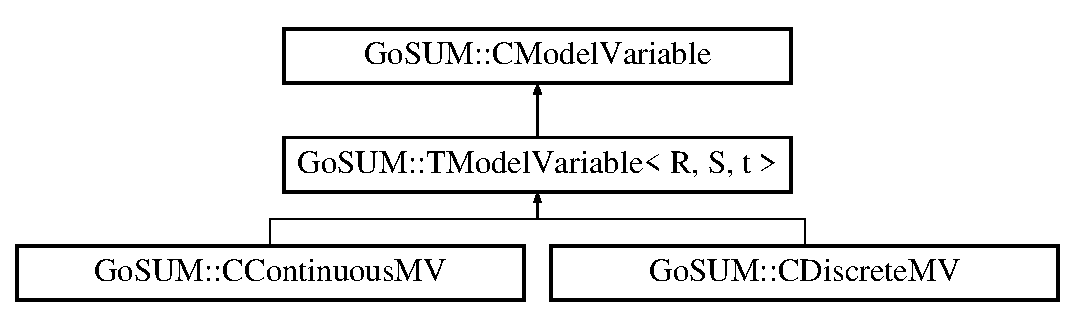
\includegraphics[height=3.000000cm]{class_go_s_u_m_1_1_c_model_variable}
\end{center}
\end{figure}
\subsection*{Public Member Functions}
\begin{DoxyCompactItemize}
\item 
\hyperlink{class_go_s_u_m_1_1_c_model_variable_af87a883a7decdacb83591c41817a0a12}{C\-Model\-Variable} ()
\item 
virtual \hyperlink{class_go_s_u_m_1_1_c_model_variable_a54604e01443f4195b1ea3a197458dc07}{$\sim$\-C\-Model\-Variable} ()
\item 
\hyperlink{class_go_s_u_m_1_1_c_model_variable}{C\-Model\-Variable} $\ast$ \hyperlink{class_go_s_u_m_1_1_c_model_variable_ab70398d40549692929f1bfbff7281a56}{clone} (std\-::string \-\_\-uname)
\begin{DoxyCompactList}\small\item\em Clones itself to a new model variable with different name. \end{DoxyCompactList}\item 
void \hyperlink{class_go_s_u_m_1_1_c_model_variable_a2166acba16fad9f71f3fcf8b1f8cebb2}{set\-Name} (const std\-::string \&\-\_\-uname)
\begin{DoxyCompactList}\small\item\em Set name of the model variable. \end{DoxyCompactList}\item 
std\-::string \hyperlink{class_go_s_u_m_1_1_c_model_variable_ae305b19e3e4705db2a0c989b45dd58f9}{name} () const 
\begin{DoxyCompactList}\small\item\em Returns name of the model variable. \end{DoxyCompactList}\item 
virtual void \hyperlink{class_go_s_u_m_1_1_c_model_variable_af53c01e36cd1b8fdfec4e66a99776745}{clear\-Sample} ()=0
\begin{DoxyCompactList}\small\item\em Clears variable's sample. \end{DoxyCompactList}\item 
virtual int \hyperlink{class_go_s_u_m_1_1_c_model_variable_ab2889a825983ec58f9661a1e162904f3}{expanded\-Size} () const =0
\item 
virtual void \hyperlink{class_go_s_u_m_1_1_c_model_variable_a4424193dc952f62acaa2bb902b1585cd}{set\-Sample\-Size} (int \-\_\-n)=0
\begin{DoxyCompactList}\small\item\em Returns number of variables after expansion for analytical model. \end{DoxyCompactList}\item 
virtual int \hyperlink{class_go_s_u_m_1_1_c_model_variable_a6119dc5693874222727b2c2e24c7494d}{sample\-Size} () const =0
\begin{DoxyCompactList}\small\item\em Returns sample size. \end{DoxyCompactList}\item 
virtual void \hyperlink{class_go_s_u_m_1_1_c_model_variable_a08f9738a6142029c5e9f0609a171c8c5}{set\-Sample\-Value} (double \-\_\-val, int \-\_\-at)=0
\begin{DoxyCompactList}\small\item\em Sets particular sample value. \end{DoxyCompactList}\item 
virtual double \hyperlink{class_go_s_u_m_1_1_c_model_variable_aeb0c0339dee635d29b2dfea21bac6e06}{sample\-Value} (int \-\_\-at) const =0
\begin{DoxyCompactList}\small\item\em Returns particular sample value. \end{DoxyCompactList}\item 
virtual void \hyperlink{class_go_s_u_m_1_1_c_model_variable_a29c06485593cef56e0d6fc39c279feb5}{read\-Sample\-Value} (std\-::ifstream \&\-\_\-ifs, int \-\_\-at)=0
\begin{DoxyCompactList}\small\item\em Reads particular sample value from input file stream. \end{DoxyCompactList}\item 
virtual void \hyperlink{class_go_s_u_m_1_1_c_model_variable_a9de10a737f4b03f6e790e856e5822d58}{write\-Sample\-Value} (std\-::ofstream \&\-\_\-ofs, int \-\_\-at) const =0
\begin{DoxyCompactList}\small\item\em Writes particular sample value to output file stream. \end{DoxyCompactList}\item 
virtual void \hyperlink{class_go_s_u_m_1_1_c_model_variable_a9fff9e4b5f200249d1376b0890c2d132}{generate\-Sample\-Value} (double \-\_\-ranval, int \-\_\-at)=0
\begin{DoxyCompactList}\small\item\em Generates particular sample value using actual random variable model. \end{DoxyCompactList}\item 
virtual double \hyperlink{class_go_s_u_m_1_1_c_model_variable_a940f366fe5007e353cb2de3408d4d0f1}{generate\-Sample\-Value} (double \-\_\-p)=0
\begin{DoxyCompactList}\small\item\em Generates sample value using actual random variable model. \end{DoxyCompactList}\item 
virtual void \hyperlink{class_go_s_u_m_1_1_c_model_variable_afa96767d105fb9f3eb05380480b1febf}{compute\-Statistics} (int \-\_\-n)=0
\begin{DoxyCompactList}\small\item\em Computes statistics from sample (histogram, empirical mean and standard deviation etc.). \end{DoxyCompactList}\item 
virtual double \hyperlink{class_go_s_u_m_1_1_c_model_variable_a3a147e484e87534b549b44c210e8f4ec}{min\-Value} () const =0
\begin{DoxyCompactList}\small\item\em Returns minimal variable value. \end{DoxyCompactList}\item 
virtual double \hyperlink{class_go_s_u_m_1_1_c_model_variable_abf8b08388b38cffce2f8c881b257467a}{max\-Value} () const =0
\begin{DoxyCompactList}\small\item\em Returns maximal variable value. \end{DoxyCompactList}\item 
virtual double \hyperlink{class_go_s_u_m_1_1_c_model_variable_a88f89892435e7e3c2fc86a6b837415bc}{expected\-Value} () const =0
\begin{DoxyCompactList}\small\item\em Returns expected variable value. \end{DoxyCompactList}\item 
virtual void \hyperlink{class_go_s_u_m_1_1_c_model_variable_ad57110dd29c67f648825661e8ba0a3d5}{set\-Empirical\-Distribution} ()
\begin{DoxyCompactList}\small\item\em Computes distribution of the actual random variable from empirical sample data. \end{DoxyCompactList}\item 
virtual void \hyperlink{class_go_s_u_m_1_1_c_model_variable_a762505d1b3d1e36daeebfec111d221b1}{set\-Theoretical\-Distribution} ()
\begin{DoxyCompactList}\small\item\em Tests goodness-\/of-\/fit for theoretical random variables and replaces with the best that satisfies Kolomogorov-\/\-Smirnov. \end{DoxyCompactList}\item 
virtual void \hyperlink{class_go_s_u_m_1_1_c_model_variable_a7d4e06b18bd92b412112cbd8f3374d5b}{set\-Distribution} ()
\begin{DoxyCompactList}\small\item\em Computes distribution of the actual random variable from available data. \end{DoxyCompactList}\item 
virtual \\*
\hyperlink{class_c_random_variable_a80d2a87c43847274138b51f7d713d7f1}{C\-Random\-Variable\-::distributiontype} \hyperlink{class_go_s_u_m_1_1_c_model_variable_a7d8d75d0c4657a6b19ded363571bdec4}{distribution\-Type} () const =0
\begin{DoxyCompactList}\small\item\em Returns type of the random variable distribution. \end{DoxyCompactList}\item 
virtual std\-::string \hyperlink{class_go_s_u_m_1_1_c_model_variable_ab363a847d6c2c562e8f7ee22f0cf6f02}{distribution\-Name} () const =0
\begin{DoxyCompactList}\small\item\em Returns name of the random variable distribution. \end{DoxyCompactList}\item 
virtual bool \hyperlink{class_go_s_u_m_1_1_c_model_variable_a2ec4aee717249dcbad98fd6e6320a6b7}{is\-Continuous} () const =0
\begin{DoxyCompactList}\small\item\em Returns true if model variable is continuous, false otherwise. \end{DoxyCompactList}\item 
virtual bool \hyperlink{class_go_s_u_m_1_1_c_model_variable_a9d0140b610b7a1c04a3b31e2d84f86da}{is\-Discrete} () const =0
\begin{DoxyCompactList}\small\item\em Returns true if model variable is discrete, false otherwise. \end{DoxyCompactList}\item 
virtual bool \hyperlink{class_go_s_u_m_1_1_c_model_variable_a0ab50d62f624918807daef90d881c3da}{is\-Distribution\-Defined} () const =0
\begin{DoxyCompactList}\small\item\em Returns true if distribution is defined, false otherwise. \end{DoxyCompactList}\item 
\hyperlink{class_go_s_u_m_1_1_c_continuous_m_v}{C\-Continuous\-M\-V} $\ast$ \hyperlink{class_go_s_u_m_1_1_c_model_variable_a76ad39dc00e51af83d00b47a03d191a7}{cast2\-Continuous\-M\-V} ()
\begin{DoxyCompactList}\small\item\em Safe cast of model variable to \hyperlink{class_go_s_u_m_1_1_c_continuous_m_v}{C\-Continuous\-M\-V} type. \end{DoxyCompactList}\item 
\hyperlink{class_go_s_u_m_1_1_c_discrete_m_v}{C\-Discrete\-M\-V} $\ast$ \hyperlink{class_go_s_u_m_1_1_c_model_variable_a5d53861a7d2e7f9030a9a857698662da}{cast2\-Discrete\-M\-V} ()
\begin{DoxyCompactList}\small\item\em Safe cast of model variable to \hyperlink{class_go_s_u_m_1_1_c_discrete_m_v}{C\-Discrete\-M\-V} type. \end{DoxyCompactList}\item 
virtual \hyperlink{class_c_random_variable}{C\-Random\-Variable} $\ast$ \hyperlink{class_go_s_u_m_1_1_c_model_variable_ae12d28329d27f1b85085c8e0fc310739}{random\-Variable} () const =0
\begin{DoxyCompactList}\small\item\em Returns random variable. \end{DoxyCompactList}\item 
virtual \hyperlink{class_c_sample}{C\-Sample} $\ast$ \hyperlink{class_go_s_u_m_1_1_c_model_variable_a4f5739cec4081b98efc26c1c8bde690e}{sample} () const =0
\begin{DoxyCompactList}\small\item\em Returns sample. \end{DoxyCompactList}\item 
Array\-Xd \hyperlink{class_go_s_u_m_1_1_c_model_variable_a4956d33b5e6b10c2772d04db9379d467}{cast\-Export\-Sample} ()
\begin{DoxyCompactList}\small\item\em Exports model variables sample and casts it to array of doubles. \end{DoxyCompactList}\end{DoxyCompactItemize}
\subsection*{Protected Member Functions}
\begin{DoxyCompactItemize}
\item 
{\footnotesize template$<$class Archive $>$ }\\void \hyperlink{class_go_s_u_m_1_1_c_model_variable_ac65c599cd7344f263ec632db106b04f3}{serialize} (Archive \&ar, const unsigned int version)
\end{DoxyCompactItemize}
\subsection*{Protected Attributes}
\begin{DoxyCompactItemize}
\item 
std\-::string \hyperlink{class_go_s_u_m_1_1_c_model_variable_ae7476c53db1987e31c50ac89b88f5402}{uname}
\end{DoxyCompactItemize}
\subsection*{Friends}
\begin{DoxyCompactItemize}
\item 
class \hyperlink{class_go_s_u_m_1_1_c_model_variable_ac98d07dd8f7b70e16ccb9a01abf56b9c}{boost\-::serialization\-::access}
\begin{DoxyCompactList}\small\item\em Boost serialization. \end{DoxyCompactList}\end{DoxyCompactItemize}


\subsection{Detailed Description}
Class for any variable in the \hyperlink{struct_go_s_u_m}{Go\-S\-U\-M} model (input or output). 

\subsection{Constructor \& Destructor Documentation}
\hypertarget{class_go_s_u_m_1_1_c_model_variable_af87a883a7decdacb83591c41817a0a12}{\index{Go\-S\-U\-M\-::\-C\-Model\-Variable@{Go\-S\-U\-M\-::\-C\-Model\-Variable}!C\-Model\-Variable@{C\-Model\-Variable}}
\index{C\-Model\-Variable@{C\-Model\-Variable}!GoSUM::CModelVariable@{Go\-S\-U\-M\-::\-C\-Model\-Variable}}
\subsubsection[{C\-Model\-Variable}]{\setlength{\rightskip}{0pt plus 5cm}Go\-S\-U\-M\-::\-C\-Model\-Variable\-::\-C\-Model\-Variable (
\begin{DoxyParamCaption}
{}
\end{DoxyParamCaption}
)\hspace{0.3cm}{\ttfamily [inline]}}}\label{class_go_s_u_m_1_1_c_model_variable_af87a883a7decdacb83591c41817a0a12}
\hypertarget{class_go_s_u_m_1_1_c_model_variable_a54604e01443f4195b1ea3a197458dc07}{\index{Go\-S\-U\-M\-::\-C\-Model\-Variable@{Go\-S\-U\-M\-::\-C\-Model\-Variable}!$\sim$\-C\-Model\-Variable@{$\sim$\-C\-Model\-Variable}}
\index{$\sim$\-C\-Model\-Variable@{$\sim$\-C\-Model\-Variable}!GoSUM::CModelVariable@{Go\-S\-U\-M\-::\-C\-Model\-Variable}}
\subsubsection[{$\sim$\-C\-Model\-Variable}]{\setlength{\rightskip}{0pt plus 5cm}virtual Go\-S\-U\-M\-::\-C\-Model\-Variable\-::$\sim$\-C\-Model\-Variable (
\begin{DoxyParamCaption}
{}
\end{DoxyParamCaption}
)\hspace{0.3cm}{\ttfamily [inline]}, {\ttfamily [virtual]}}}\label{class_go_s_u_m_1_1_c_model_variable_a54604e01443f4195b1ea3a197458dc07}


\subsection{Member Function Documentation}
\hypertarget{class_go_s_u_m_1_1_c_model_variable_a76ad39dc00e51af83d00b47a03d191a7}{\index{Go\-S\-U\-M\-::\-C\-Model\-Variable@{Go\-S\-U\-M\-::\-C\-Model\-Variable}!cast2\-Continuous\-M\-V@{cast2\-Continuous\-M\-V}}
\index{cast2\-Continuous\-M\-V@{cast2\-Continuous\-M\-V}!GoSUM::CModelVariable@{Go\-S\-U\-M\-::\-C\-Model\-Variable}}
\subsubsection[{cast2\-Continuous\-M\-V}]{\setlength{\rightskip}{0pt plus 5cm}{\bf Go\-S\-U\-M\-::\-C\-Continuous\-M\-V} $\ast$ Go\-S\-U\-M\-::\-C\-Model\-Variable\-::cast2\-Continuous\-M\-V (
\begin{DoxyParamCaption}
{}
\end{DoxyParamCaption}
)}}\label{class_go_s_u_m_1_1_c_model_variable_a76ad39dc00e51af83d00b47a03d191a7}


Safe cast of model variable to \hyperlink{class_go_s_u_m_1_1_c_continuous_m_v}{C\-Continuous\-M\-V} type. 

\hypertarget{class_go_s_u_m_1_1_c_model_variable_a5d53861a7d2e7f9030a9a857698662da}{\index{Go\-S\-U\-M\-::\-C\-Model\-Variable@{Go\-S\-U\-M\-::\-C\-Model\-Variable}!cast2\-Discrete\-M\-V@{cast2\-Discrete\-M\-V}}
\index{cast2\-Discrete\-M\-V@{cast2\-Discrete\-M\-V}!GoSUM::CModelVariable@{Go\-S\-U\-M\-::\-C\-Model\-Variable}}
\subsubsection[{cast2\-Discrete\-M\-V}]{\setlength{\rightskip}{0pt plus 5cm}{\bf Go\-S\-U\-M\-::\-C\-Discrete\-M\-V} $\ast$ Go\-S\-U\-M\-::\-C\-Model\-Variable\-::cast2\-Discrete\-M\-V (
\begin{DoxyParamCaption}
{}
\end{DoxyParamCaption}
)}}\label{class_go_s_u_m_1_1_c_model_variable_a5d53861a7d2e7f9030a9a857698662da}


Safe cast of model variable to \hyperlink{class_go_s_u_m_1_1_c_discrete_m_v}{C\-Discrete\-M\-V} type. 

\hypertarget{class_go_s_u_m_1_1_c_model_variable_a4956d33b5e6b10c2772d04db9379d467}{\index{Go\-S\-U\-M\-::\-C\-Model\-Variable@{Go\-S\-U\-M\-::\-C\-Model\-Variable}!cast\-Export\-Sample@{cast\-Export\-Sample}}
\index{cast\-Export\-Sample@{cast\-Export\-Sample}!GoSUM::CModelVariable@{Go\-S\-U\-M\-::\-C\-Model\-Variable}}
\subsubsection[{cast\-Export\-Sample}]{\setlength{\rightskip}{0pt plus 5cm}Array\-Xd Go\-S\-U\-M\-::\-C\-Model\-Variable\-::cast\-Export\-Sample (
\begin{DoxyParamCaption}
{}
\end{DoxyParamCaption}
)}}\label{class_go_s_u_m_1_1_c_model_variable_a4956d33b5e6b10c2772d04db9379d467}


Exports model variables sample and casts it to array of doubles. 

\hypertarget{class_go_s_u_m_1_1_c_model_variable_af53c01e36cd1b8fdfec4e66a99776745}{\index{Go\-S\-U\-M\-::\-C\-Model\-Variable@{Go\-S\-U\-M\-::\-C\-Model\-Variable}!clear\-Sample@{clear\-Sample}}
\index{clear\-Sample@{clear\-Sample}!GoSUM::CModelVariable@{Go\-S\-U\-M\-::\-C\-Model\-Variable}}
\subsubsection[{clear\-Sample}]{\setlength{\rightskip}{0pt plus 5cm}virtual void Go\-S\-U\-M\-::\-C\-Model\-Variable\-::clear\-Sample (
\begin{DoxyParamCaption}
{}
\end{DoxyParamCaption}
)\hspace{0.3cm}{\ttfamily [pure virtual]}}}\label{class_go_s_u_m_1_1_c_model_variable_af53c01e36cd1b8fdfec4e66a99776745}


Clears variable's sample. 



Implemented in \hyperlink{class_go_s_u_m_1_1_t_model_variable_a92694058f7f782f6e7302f1130f1f174}{Go\-S\-U\-M\-::\-T\-Model\-Variable$<$ R, S, t $>$}.

\hypertarget{class_go_s_u_m_1_1_c_model_variable_ab70398d40549692929f1bfbff7281a56}{\index{Go\-S\-U\-M\-::\-C\-Model\-Variable@{Go\-S\-U\-M\-::\-C\-Model\-Variable}!clone@{clone}}
\index{clone@{clone}!GoSUM::CModelVariable@{Go\-S\-U\-M\-::\-C\-Model\-Variable}}
\subsubsection[{clone}]{\setlength{\rightskip}{0pt plus 5cm}{\bf Go\-S\-U\-M\-::\-C\-Model\-Variable} $\ast$ Go\-S\-U\-M\-::\-C\-Model\-Variable\-::clone (
\begin{DoxyParamCaption}
\item[{std\-::string}]{\-\_\-uname}
\end{DoxyParamCaption}
)}}\label{class_go_s_u_m_1_1_c_model_variable_ab70398d40549692929f1bfbff7281a56}


Clones itself to a new model variable with different name. 

\hypertarget{class_go_s_u_m_1_1_c_model_variable_afa96767d105fb9f3eb05380480b1febf}{\index{Go\-S\-U\-M\-::\-C\-Model\-Variable@{Go\-S\-U\-M\-::\-C\-Model\-Variable}!compute\-Statistics@{compute\-Statistics}}
\index{compute\-Statistics@{compute\-Statistics}!GoSUM::CModelVariable@{Go\-S\-U\-M\-::\-C\-Model\-Variable}}
\subsubsection[{compute\-Statistics}]{\setlength{\rightskip}{0pt plus 5cm}virtual void Go\-S\-U\-M\-::\-C\-Model\-Variable\-::compute\-Statistics (
\begin{DoxyParamCaption}
\item[{int}]{\-\_\-n}
\end{DoxyParamCaption}
)\hspace{0.3cm}{\ttfamily [pure virtual]}}}\label{class_go_s_u_m_1_1_c_model_variable_afa96767d105fb9f3eb05380480b1febf}


Computes statistics from sample (histogram, empirical mean and standard deviation etc.). 



Implemented in \hyperlink{class_go_s_u_m_1_1_t_model_variable_ad1995ed1abea87ed8678f65659cf7a64}{Go\-S\-U\-M\-::\-T\-Model\-Variable$<$ R, S, t $>$}.

\hypertarget{class_go_s_u_m_1_1_c_model_variable_ab363a847d6c2c562e8f7ee22f0cf6f02}{\index{Go\-S\-U\-M\-::\-C\-Model\-Variable@{Go\-S\-U\-M\-::\-C\-Model\-Variable}!distribution\-Name@{distribution\-Name}}
\index{distribution\-Name@{distribution\-Name}!GoSUM::CModelVariable@{Go\-S\-U\-M\-::\-C\-Model\-Variable}}
\subsubsection[{distribution\-Name}]{\setlength{\rightskip}{0pt plus 5cm}virtual std\-::string Go\-S\-U\-M\-::\-C\-Model\-Variable\-::distribution\-Name (
\begin{DoxyParamCaption}
{}
\end{DoxyParamCaption}
) const\hspace{0.3cm}{\ttfamily [pure virtual]}}}\label{class_go_s_u_m_1_1_c_model_variable_ab363a847d6c2c562e8f7ee22f0cf6f02}


Returns name of the random variable distribution. 



Implemented in \hyperlink{class_go_s_u_m_1_1_t_model_variable_aa41c0ebb9c0e5dfbb98c2ea66a77890d}{Go\-S\-U\-M\-::\-T\-Model\-Variable$<$ R, S, t $>$}.

\hypertarget{class_go_s_u_m_1_1_c_model_variable_a7d8d75d0c4657a6b19ded363571bdec4}{\index{Go\-S\-U\-M\-::\-C\-Model\-Variable@{Go\-S\-U\-M\-::\-C\-Model\-Variable}!distribution\-Type@{distribution\-Type}}
\index{distribution\-Type@{distribution\-Type}!GoSUM::CModelVariable@{Go\-S\-U\-M\-::\-C\-Model\-Variable}}
\subsubsection[{distribution\-Type}]{\setlength{\rightskip}{0pt plus 5cm}virtual {\bf C\-Random\-Variable\-::distributiontype} Go\-S\-U\-M\-::\-C\-Model\-Variable\-::distribution\-Type (
\begin{DoxyParamCaption}
{}
\end{DoxyParamCaption}
) const\hspace{0.3cm}{\ttfamily [pure virtual]}}}\label{class_go_s_u_m_1_1_c_model_variable_a7d8d75d0c4657a6b19ded363571bdec4}


Returns type of the random variable distribution. 



Implemented in \hyperlink{class_go_s_u_m_1_1_t_model_variable_a8dea19600fc9455dadd31a79c539e82e}{Go\-S\-U\-M\-::\-T\-Model\-Variable$<$ R, S, t $>$}.

\hypertarget{class_go_s_u_m_1_1_c_model_variable_ab2889a825983ec58f9661a1e162904f3}{\index{Go\-S\-U\-M\-::\-C\-Model\-Variable@{Go\-S\-U\-M\-::\-C\-Model\-Variable}!expanded\-Size@{expanded\-Size}}
\index{expanded\-Size@{expanded\-Size}!GoSUM::CModelVariable@{Go\-S\-U\-M\-::\-C\-Model\-Variable}}
\subsubsection[{expanded\-Size}]{\setlength{\rightskip}{0pt plus 5cm}virtual int Go\-S\-U\-M\-::\-C\-Model\-Variable\-::expanded\-Size (
\begin{DoxyParamCaption}
{}
\end{DoxyParamCaption}
) const\hspace{0.3cm}{\ttfamily [pure virtual]}}}\label{class_go_s_u_m_1_1_c_model_variable_ab2889a825983ec58f9661a1e162904f3}


Implemented in \hyperlink{class_go_s_u_m_1_1_t_model_variable_ae00e5653833fcf6f8d05c24d4cff741d}{Go\-S\-U\-M\-::\-T\-Model\-Variable$<$ R, S, t $>$}.

\hypertarget{class_go_s_u_m_1_1_c_model_variable_a88f89892435e7e3c2fc86a6b837415bc}{\index{Go\-S\-U\-M\-::\-C\-Model\-Variable@{Go\-S\-U\-M\-::\-C\-Model\-Variable}!expected\-Value@{expected\-Value}}
\index{expected\-Value@{expected\-Value}!GoSUM::CModelVariable@{Go\-S\-U\-M\-::\-C\-Model\-Variable}}
\subsubsection[{expected\-Value}]{\setlength{\rightskip}{0pt plus 5cm}virtual double Go\-S\-U\-M\-::\-C\-Model\-Variable\-::expected\-Value (
\begin{DoxyParamCaption}
{}
\end{DoxyParamCaption}
) const\hspace{0.3cm}{\ttfamily [pure virtual]}}}\label{class_go_s_u_m_1_1_c_model_variable_a88f89892435e7e3c2fc86a6b837415bc}


Returns expected variable value. 



Implemented in \hyperlink{class_go_s_u_m_1_1_t_model_variable_a6bdec5497c51d855daccf9033927b8bc}{Go\-S\-U\-M\-::\-T\-Model\-Variable$<$ R, S, t $>$}.

\hypertarget{class_go_s_u_m_1_1_c_model_variable_a9fff9e4b5f200249d1376b0890c2d132}{\index{Go\-S\-U\-M\-::\-C\-Model\-Variable@{Go\-S\-U\-M\-::\-C\-Model\-Variable}!generate\-Sample\-Value@{generate\-Sample\-Value}}
\index{generate\-Sample\-Value@{generate\-Sample\-Value}!GoSUM::CModelVariable@{Go\-S\-U\-M\-::\-C\-Model\-Variable}}
\subsubsection[{generate\-Sample\-Value}]{\setlength{\rightskip}{0pt plus 5cm}virtual void Go\-S\-U\-M\-::\-C\-Model\-Variable\-::generate\-Sample\-Value (
\begin{DoxyParamCaption}
\item[{double}]{\-\_\-ranval, }
\item[{int}]{\-\_\-at}
\end{DoxyParamCaption}
)\hspace{0.3cm}{\ttfamily [pure virtual]}}}\label{class_go_s_u_m_1_1_c_model_variable_a9fff9e4b5f200249d1376b0890c2d132}


Generates particular sample value using actual random variable model. 



Implemented in \hyperlink{class_go_s_u_m_1_1_t_model_variable_a94c22ba7a540482c9f38ca5f00d9a755}{Go\-S\-U\-M\-::\-T\-Model\-Variable$<$ R, S, t $>$}.

\hypertarget{class_go_s_u_m_1_1_c_model_variable_a940f366fe5007e353cb2de3408d4d0f1}{\index{Go\-S\-U\-M\-::\-C\-Model\-Variable@{Go\-S\-U\-M\-::\-C\-Model\-Variable}!generate\-Sample\-Value@{generate\-Sample\-Value}}
\index{generate\-Sample\-Value@{generate\-Sample\-Value}!GoSUM::CModelVariable@{Go\-S\-U\-M\-::\-C\-Model\-Variable}}
\subsubsection[{generate\-Sample\-Value}]{\setlength{\rightskip}{0pt plus 5cm}virtual double Go\-S\-U\-M\-::\-C\-Model\-Variable\-::generate\-Sample\-Value (
\begin{DoxyParamCaption}
\item[{double}]{\-\_\-p}
\end{DoxyParamCaption}
)\hspace{0.3cm}{\ttfamily [pure virtual]}}}\label{class_go_s_u_m_1_1_c_model_variable_a940f366fe5007e353cb2de3408d4d0f1}


Generates sample value using actual random variable model. 



Implemented in \hyperlink{class_go_s_u_m_1_1_t_model_variable_a5ebe0e2a02aa1a98fa2442865170a2f5}{Go\-S\-U\-M\-::\-T\-Model\-Variable$<$ R, S, t $>$}.

\hypertarget{class_go_s_u_m_1_1_c_model_variable_a2ec4aee717249dcbad98fd6e6320a6b7}{\index{Go\-S\-U\-M\-::\-C\-Model\-Variable@{Go\-S\-U\-M\-::\-C\-Model\-Variable}!is\-Continuous@{is\-Continuous}}
\index{is\-Continuous@{is\-Continuous}!GoSUM::CModelVariable@{Go\-S\-U\-M\-::\-C\-Model\-Variable}}
\subsubsection[{is\-Continuous}]{\setlength{\rightskip}{0pt plus 5cm}virtual bool Go\-S\-U\-M\-::\-C\-Model\-Variable\-::is\-Continuous (
\begin{DoxyParamCaption}
{}
\end{DoxyParamCaption}
) const\hspace{0.3cm}{\ttfamily [pure virtual]}}}\label{class_go_s_u_m_1_1_c_model_variable_a2ec4aee717249dcbad98fd6e6320a6b7}


Returns true if model variable is continuous, false otherwise. 



Implemented in \hyperlink{class_go_s_u_m_1_1_c_continuous_m_v_a8f523f36ccdecfb58d468b6976890b15}{Go\-S\-U\-M\-::\-C\-Continuous\-M\-V}, and \hyperlink{class_go_s_u_m_1_1_c_discrete_m_v_a6366f6f6fd00242942b733ef5715592e}{Go\-S\-U\-M\-::\-C\-Discrete\-M\-V}.

\hypertarget{class_go_s_u_m_1_1_c_model_variable_a9d0140b610b7a1c04a3b31e2d84f86da}{\index{Go\-S\-U\-M\-::\-C\-Model\-Variable@{Go\-S\-U\-M\-::\-C\-Model\-Variable}!is\-Discrete@{is\-Discrete}}
\index{is\-Discrete@{is\-Discrete}!GoSUM::CModelVariable@{Go\-S\-U\-M\-::\-C\-Model\-Variable}}
\subsubsection[{is\-Discrete}]{\setlength{\rightskip}{0pt plus 5cm}virtual bool Go\-S\-U\-M\-::\-C\-Model\-Variable\-::is\-Discrete (
\begin{DoxyParamCaption}
{}
\end{DoxyParamCaption}
) const\hspace{0.3cm}{\ttfamily [pure virtual]}}}\label{class_go_s_u_m_1_1_c_model_variable_a9d0140b610b7a1c04a3b31e2d84f86da}


Returns true if model variable is discrete, false otherwise. 



Implemented in \hyperlink{class_go_s_u_m_1_1_c_continuous_m_v_aeaef5939c27a7e074c33f783d73484a5}{Go\-S\-U\-M\-::\-C\-Continuous\-M\-V}, and \hyperlink{class_go_s_u_m_1_1_c_discrete_m_v_ad9da78f518019e7133440189803f9cad}{Go\-S\-U\-M\-::\-C\-Discrete\-M\-V}.

\hypertarget{class_go_s_u_m_1_1_c_model_variable_a0ab50d62f624918807daef90d881c3da}{\index{Go\-S\-U\-M\-::\-C\-Model\-Variable@{Go\-S\-U\-M\-::\-C\-Model\-Variable}!is\-Distribution\-Defined@{is\-Distribution\-Defined}}
\index{is\-Distribution\-Defined@{is\-Distribution\-Defined}!GoSUM::CModelVariable@{Go\-S\-U\-M\-::\-C\-Model\-Variable}}
\subsubsection[{is\-Distribution\-Defined}]{\setlength{\rightskip}{0pt plus 5cm}virtual bool Go\-S\-U\-M\-::\-C\-Model\-Variable\-::is\-Distribution\-Defined (
\begin{DoxyParamCaption}
{}
\end{DoxyParamCaption}
) const\hspace{0.3cm}{\ttfamily [pure virtual]}}}\label{class_go_s_u_m_1_1_c_model_variable_a0ab50d62f624918807daef90d881c3da}


Returns true if distribution is defined, false otherwise. 



Implemented in \hyperlink{class_go_s_u_m_1_1_t_model_variable_a49e8bb3711a10e298e90cb6a8d12661a}{Go\-S\-U\-M\-::\-T\-Model\-Variable$<$ R, S, t $>$}.

\hypertarget{class_go_s_u_m_1_1_c_model_variable_abf8b08388b38cffce2f8c881b257467a}{\index{Go\-S\-U\-M\-::\-C\-Model\-Variable@{Go\-S\-U\-M\-::\-C\-Model\-Variable}!max\-Value@{max\-Value}}
\index{max\-Value@{max\-Value}!GoSUM::CModelVariable@{Go\-S\-U\-M\-::\-C\-Model\-Variable}}
\subsubsection[{max\-Value}]{\setlength{\rightskip}{0pt plus 5cm}virtual double Go\-S\-U\-M\-::\-C\-Model\-Variable\-::max\-Value (
\begin{DoxyParamCaption}
{}
\end{DoxyParamCaption}
) const\hspace{0.3cm}{\ttfamily [pure virtual]}}}\label{class_go_s_u_m_1_1_c_model_variable_abf8b08388b38cffce2f8c881b257467a}


Returns maximal variable value. 



Implemented in \hyperlink{class_go_s_u_m_1_1_t_model_variable_a0d9ad1fc30fde0f3dd7ba204f1b525a2}{Go\-S\-U\-M\-::\-T\-Model\-Variable$<$ R, S, t $>$}.

\hypertarget{class_go_s_u_m_1_1_c_model_variable_a3a147e484e87534b549b44c210e8f4ec}{\index{Go\-S\-U\-M\-::\-C\-Model\-Variable@{Go\-S\-U\-M\-::\-C\-Model\-Variable}!min\-Value@{min\-Value}}
\index{min\-Value@{min\-Value}!GoSUM::CModelVariable@{Go\-S\-U\-M\-::\-C\-Model\-Variable}}
\subsubsection[{min\-Value}]{\setlength{\rightskip}{0pt plus 5cm}virtual double Go\-S\-U\-M\-::\-C\-Model\-Variable\-::min\-Value (
\begin{DoxyParamCaption}
{}
\end{DoxyParamCaption}
) const\hspace{0.3cm}{\ttfamily [pure virtual]}}}\label{class_go_s_u_m_1_1_c_model_variable_a3a147e484e87534b549b44c210e8f4ec}


Returns minimal variable value. 



Implemented in \hyperlink{class_go_s_u_m_1_1_t_model_variable_a0395e6699e577b7ccb77e19787adc169}{Go\-S\-U\-M\-::\-T\-Model\-Variable$<$ R, S, t $>$}.

\hypertarget{class_go_s_u_m_1_1_c_model_variable_ae305b19e3e4705db2a0c989b45dd58f9}{\index{Go\-S\-U\-M\-::\-C\-Model\-Variable@{Go\-S\-U\-M\-::\-C\-Model\-Variable}!name@{name}}
\index{name@{name}!GoSUM::CModelVariable@{Go\-S\-U\-M\-::\-C\-Model\-Variable}}
\subsubsection[{name}]{\setlength{\rightskip}{0pt plus 5cm}std\-::string Go\-S\-U\-M\-::\-C\-Model\-Variable\-::name (
\begin{DoxyParamCaption}
{}
\end{DoxyParamCaption}
) const\hspace{0.3cm}{\ttfamily [inline]}}}\label{class_go_s_u_m_1_1_c_model_variable_ae305b19e3e4705db2a0c989b45dd58f9}


Returns name of the model variable. 

\hypertarget{class_go_s_u_m_1_1_c_model_variable_ae12d28329d27f1b85085c8e0fc310739}{\index{Go\-S\-U\-M\-::\-C\-Model\-Variable@{Go\-S\-U\-M\-::\-C\-Model\-Variable}!random\-Variable@{random\-Variable}}
\index{random\-Variable@{random\-Variable}!GoSUM::CModelVariable@{Go\-S\-U\-M\-::\-C\-Model\-Variable}}
\subsubsection[{random\-Variable}]{\setlength{\rightskip}{0pt plus 5cm}virtual {\bf C\-Random\-Variable}$\ast$ Go\-S\-U\-M\-::\-C\-Model\-Variable\-::random\-Variable (
\begin{DoxyParamCaption}
{}
\end{DoxyParamCaption}
) const\hspace{0.3cm}{\ttfamily [pure virtual]}}}\label{class_go_s_u_m_1_1_c_model_variable_ae12d28329d27f1b85085c8e0fc310739}


Returns random variable. 



Implemented in \hyperlink{class_go_s_u_m_1_1_t_model_variable_a8d74a8298078d6d99f62da8ea096e359}{Go\-S\-U\-M\-::\-T\-Model\-Variable$<$ R, S, t $>$}.

\hypertarget{class_go_s_u_m_1_1_c_model_variable_a29c06485593cef56e0d6fc39c279feb5}{\index{Go\-S\-U\-M\-::\-C\-Model\-Variable@{Go\-S\-U\-M\-::\-C\-Model\-Variable}!read\-Sample\-Value@{read\-Sample\-Value}}
\index{read\-Sample\-Value@{read\-Sample\-Value}!GoSUM::CModelVariable@{Go\-S\-U\-M\-::\-C\-Model\-Variable}}
\subsubsection[{read\-Sample\-Value}]{\setlength{\rightskip}{0pt plus 5cm}virtual void Go\-S\-U\-M\-::\-C\-Model\-Variable\-::read\-Sample\-Value (
\begin{DoxyParamCaption}
\item[{std\-::ifstream \&}]{\-\_\-ifs, }
\item[{int}]{\-\_\-at}
\end{DoxyParamCaption}
)\hspace{0.3cm}{\ttfamily [pure virtual]}}}\label{class_go_s_u_m_1_1_c_model_variable_a29c06485593cef56e0d6fc39c279feb5}


Reads particular sample value from input file stream. 



Implemented in \hyperlink{class_go_s_u_m_1_1_t_model_variable_afee2c55fb595ff40904551e4a7edf360}{Go\-S\-U\-M\-::\-T\-Model\-Variable$<$ R, S, t $>$}.

\hypertarget{class_go_s_u_m_1_1_c_model_variable_a4f5739cec4081b98efc26c1c8bde690e}{\index{Go\-S\-U\-M\-::\-C\-Model\-Variable@{Go\-S\-U\-M\-::\-C\-Model\-Variable}!sample@{sample}}
\index{sample@{sample}!GoSUM::CModelVariable@{Go\-S\-U\-M\-::\-C\-Model\-Variable}}
\subsubsection[{sample}]{\setlength{\rightskip}{0pt plus 5cm}virtual {\bf C\-Sample}$\ast$ Go\-S\-U\-M\-::\-C\-Model\-Variable\-::sample (
\begin{DoxyParamCaption}
{}
\end{DoxyParamCaption}
) const\hspace{0.3cm}{\ttfamily [pure virtual]}}}\label{class_go_s_u_m_1_1_c_model_variable_a4f5739cec4081b98efc26c1c8bde690e}


Returns sample. 



Implemented in \hyperlink{class_go_s_u_m_1_1_t_model_variable_ad7699e50c6f2a7b67ff9e178fe1af740}{Go\-S\-U\-M\-::\-T\-Model\-Variable$<$ R, S, t $>$}.

\hypertarget{class_go_s_u_m_1_1_c_model_variable_a6119dc5693874222727b2c2e24c7494d}{\index{Go\-S\-U\-M\-::\-C\-Model\-Variable@{Go\-S\-U\-M\-::\-C\-Model\-Variable}!sample\-Size@{sample\-Size}}
\index{sample\-Size@{sample\-Size}!GoSUM::CModelVariable@{Go\-S\-U\-M\-::\-C\-Model\-Variable}}
\subsubsection[{sample\-Size}]{\setlength{\rightskip}{0pt plus 5cm}virtual int Go\-S\-U\-M\-::\-C\-Model\-Variable\-::sample\-Size (
\begin{DoxyParamCaption}
{}
\end{DoxyParamCaption}
) const\hspace{0.3cm}{\ttfamily [pure virtual]}}}\label{class_go_s_u_m_1_1_c_model_variable_a6119dc5693874222727b2c2e24c7494d}


Returns sample size. 



Implemented in \hyperlink{class_go_s_u_m_1_1_t_model_variable_a4c63e42e4ec1971dc9d5671785071426}{Go\-S\-U\-M\-::\-T\-Model\-Variable$<$ R, S, t $>$}.

\hypertarget{class_go_s_u_m_1_1_c_model_variable_aeb0c0339dee635d29b2dfea21bac6e06}{\index{Go\-S\-U\-M\-::\-C\-Model\-Variable@{Go\-S\-U\-M\-::\-C\-Model\-Variable}!sample\-Value@{sample\-Value}}
\index{sample\-Value@{sample\-Value}!GoSUM::CModelVariable@{Go\-S\-U\-M\-::\-C\-Model\-Variable}}
\subsubsection[{sample\-Value}]{\setlength{\rightskip}{0pt plus 5cm}virtual double Go\-S\-U\-M\-::\-C\-Model\-Variable\-::sample\-Value (
\begin{DoxyParamCaption}
\item[{int}]{\-\_\-at}
\end{DoxyParamCaption}
) const\hspace{0.3cm}{\ttfamily [pure virtual]}}}\label{class_go_s_u_m_1_1_c_model_variable_aeb0c0339dee635d29b2dfea21bac6e06}


Returns particular sample value. 



Implemented in \hyperlink{class_go_s_u_m_1_1_t_model_variable_ae851745a4f6ec2f6655adcbbc83ff8c5}{Go\-S\-U\-M\-::\-T\-Model\-Variable$<$ R, S, t $>$}.

\hypertarget{class_go_s_u_m_1_1_c_model_variable_ac65c599cd7344f263ec632db106b04f3}{\index{Go\-S\-U\-M\-::\-C\-Model\-Variable@{Go\-S\-U\-M\-::\-C\-Model\-Variable}!serialize@{serialize}}
\index{serialize@{serialize}!GoSUM::CModelVariable@{Go\-S\-U\-M\-::\-C\-Model\-Variable}}
\subsubsection[{serialize}]{\setlength{\rightskip}{0pt plus 5cm}template$<$class Archive $>$ void Go\-S\-U\-M\-::\-C\-Model\-Variable\-::serialize (
\begin{DoxyParamCaption}
\item[{Archive \&}]{ar, }
\item[{const unsigned int}]{version}
\end{DoxyParamCaption}
)\hspace{0.3cm}{\ttfamily [inline]}, {\ttfamily [protected]}}}\label{class_go_s_u_m_1_1_c_model_variable_ac65c599cd7344f263ec632db106b04f3}


Reimplemented in \hyperlink{class_go_s_u_m_1_1_t_model_variable_a0a5c395a4ff28acc07f8e5670ff9d289}{Go\-S\-U\-M\-::\-T\-Model\-Variable$<$ R, S, t $>$}.

\hypertarget{class_go_s_u_m_1_1_c_model_variable_a7d4e06b18bd92b412112cbd8f3374d5b}{\index{Go\-S\-U\-M\-::\-C\-Model\-Variable@{Go\-S\-U\-M\-::\-C\-Model\-Variable}!set\-Distribution@{set\-Distribution}}
\index{set\-Distribution@{set\-Distribution}!GoSUM::CModelVariable@{Go\-S\-U\-M\-::\-C\-Model\-Variable}}
\subsubsection[{set\-Distribution}]{\setlength{\rightskip}{0pt plus 5cm}virtual void Go\-S\-U\-M\-::\-C\-Model\-Variable\-::set\-Distribution (
\begin{DoxyParamCaption}
{}
\end{DoxyParamCaption}
)\hspace{0.3cm}{\ttfamily [inline]}, {\ttfamily [virtual]}}}\label{class_go_s_u_m_1_1_c_model_variable_a7d4e06b18bd92b412112cbd8f3374d5b}


Computes distribution of the actual random variable from available data. 

\hypertarget{class_go_s_u_m_1_1_c_model_variable_ad57110dd29c67f648825661e8ba0a3d5}{\index{Go\-S\-U\-M\-::\-C\-Model\-Variable@{Go\-S\-U\-M\-::\-C\-Model\-Variable}!set\-Empirical\-Distribution@{set\-Empirical\-Distribution}}
\index{set\-Empirical\-Distribution@{set\-Empirical\-Distribution}!GoSUM::CModelVariable@{Go\-S\-U\-M\-::\-C\-Model\-Variable}}
\subsubsection[{set\-Empirical\-Distribution}]{\setlength{\rightskip}{0pt plus 5cm}virtual void Go\-S\-U\-M\-::\-C\-Model\-Variable\-::set\-Empirical\-Distribution (
\begin{DoxyParamCaption}
{}
\end{DoxyParamCaption}
)\hspace{0.3cm}{\ttfamily [inline]}, {\ttfamily [virtual]}}}\label{class_go_s_u_m_1_1_c_model_variable_ad57110dd29c67f648825661e8ba0a3d5}


Computes distribution of the actual random variable from empirical sample data. 



Reimplemented in \hyperlink{class_go_s_u_m_1_1_c_continuous_m_v_a65b0b9b16980f16fe2bc36bf8d79e3b9}{Go\-S\-U\-M\-::\-C\-Continuous\-M\-V}, \hyperlink{class_go_s_u_m_1_1_c_discrete_m_v_a7dd5ab7ac4922cdb2682012c942e1f10}{Go\-S\-U\-M\-::\-C\-Discrete\-M\-V}, and \hyperlink{class_go_s_u_m_1_1_t_model_variable_a3128d12e3ce0757714a7596de087314e}{Go\-S\-U\-M\-::\-T\-Model\-Variable$<$ R, S, t $>$}.

\hypertarget{class_go_s_u_m_1_1_c_model_variable_a2166acba16fad9f71f3fcf8b1f8cebb2}{\index{Go\-S\-U\-M\-::\-C\-Model\-Variable@{Go\-S\-U\-M\-::\-C\-Model\-Variable}!set\-Name@{set\-Name}}
\index{set\-Name@{set\-Name}!GoSUM::CModelVariable@{Go\-S\-U\-M\-::\-C\-Model\-Variable}}
\subsubsection[{set\-Name}]{\setlength{\rightskip}{0pt plus 5cm}void Go\-S\-U\-M\-::\-C\-Model\-Variable\-::set\-Name (
\begin{DoxyParamCaption}
\item[{const std\-::string \&}]{\-\_\-uname}
\end{DoxyParamCaption}
)\hspace{0.3cm}{\ttfamily [inline]}}}\label{class_go_s_u_m_1_1_c_model_variable_a2166acba16fad9f71f3fcf8b1f8cebb2}


Set name of the model variable. 

\hypertarget{class_go_s_u_m_1_1_c_model_variable_a4424193dc952f62acaa2bb902b1585cd}{\index{Go\-S\-U\-M\-::\-C\-Model\-Variable@{Go\-S\-U\-M\-::\-C\-Model\-Variable}!set\-Sample\-Size@{set\-Sample\-Size}}
\index{set\-Sample\-Size@{set\-Sample\-Size}!GoSUM::CModelVariable@{Go\-S\-U\-M\-::\-C\-Model\-Variable}}
\subsubsection[{set\-Sample\-Size}]{\setlength{\rightskip}{0pt plus 5cm}virtual void Go\-S\-U\-M\-::\-C\-Model\-Variable\-::set\-Sample\-Size (
\begin{DoxyParamCaption}
\item[{int}]{\-\_\-n}
\end{DoxyParamCaption}
)\hspace{0.3cm}{\ttfamily [pure virtual]}}}\label{class_go_s_u_m_1_1_c_model_variable_a4424193dc952f62acaa2bb902b1585cd}


Returns number of variables after expansion for analytical model. 

Sets sample size. 

Implemented in \hyperlink{class_go_s_u_m_1_1_t_model_variable_aa172b11eba6fd1819f10a80d95fc4877}{Go\-S\-U\-M\-::\-T\-Model\-Variable$<$ R, S, t $>$}.

\hypertarget{class_go_s_u_m_1_1_c_model_variable_a08f9738a6142029c5e9f0609a171c8c5}{\index{Go\-S\-U\-M\-::\-C\-Model\-Variable@{Go\-S\-U\-M\-::\-C\-Model\-Variable}!set\-Sample\-Value@{set\-Sample\-Value}}
\index{set\-Sample\-Value@{set\-Sample\-Value}!GoSUM::CModelVariable@{Go\-S\-U\-M\-::\-C\-Model\-Variable}}
\subsubsection[{set\-Sample\-Value}]{\setlength{\rightskip}{0pt plus 5cm}virtual void Go\-S\-U\-M\-::\-C\-Model\-Variable\-::set\-Sample\-Value (
\begin{DoxyParamCaption}
\item[{double}]{\-\_\-val, }
\item[{int}]{\-\_\-at}
\end{DoxyParamCaption}
)\hspace{0.3cm}{\ttfamily [pure virtual]}}}\label{class_go_s_u_m_1_1_c_model_variable_a08f9738a6142029c5e9f0609a171c8c5}


Sets particular sample value. 



Implemented in \hyperlink{class_go_s_u_m_1_1_t_model_variable_acc9cdd0db3d7bc217ae68da7bd6de737}{Go\-S\-U\-M\-::\-T\-Model\-Variable$<$ R, S, t $>$}.

\hypertarget{class_go_s_u_m_1_1_c_model_variable_a762505d1b3d1e36daeebfec111d221b1}{\index{Go\-S\-U\-M\-::\-C\-Model\-Variable@{Go\-S\-U\-M\-::\-C\-Model\-Variable}!set\-Theoretical\-Distribution@{set\-Theoretical\-Distribution}}
\index{set\-Theoretical\-Distribution@{set\-Theoretical\-Distribution}!GoSUM::CModelVariable@{Go\-S\-U\-M\-::\-C\-Model\-Variable}}
\subsubsection[{set\-Theoretical\-Distribution}]{\setlength{\rightskip}{0pt plus 5cm}virtual void Go\-S\-U\-M\-::\-C\-Model\-Variable\-::set\-Theoretical\-Distribution (
\begin{DoxyParamCaption}
{}
\end{DoxyParamCaption}
)\hspace{0.3cm}{\ttfamily [inline]}, {\ttfamily [virtual]}}}\label{class_go_s_u_m_1_1_c_model_variable_a762505d1b3d1e36daeebfec111d221b1}


Tests goodness-\/of-\/fit for theoretical random variables and replaces with the best that satisfies Kolomogorov-\/\-Smirnov. 



Reimplemented in \hyperlink{class_go_s_u_m_1_1_c_continuous_m_v_a923c07b0735783d016b4e155b5eb0539}{Go\-S\-U\-M\-::\-C\-Continuous\-M\-V}, \hyperlink{class_go_s_u_m_1_1_c_discrete_m_v_a1061fb0a466b852ffeb111238b702b39}{Go\-S\-U\-M\-::\-C\-Discrete\-M\-V}, and \hyperlink{class_go_s_u_m_1_1_t_model_variable_ad113f33f216796f775855dd3f8553f03}{Go\-S\-U\-M\-::\-T\-Model\-Variable$<$ R, S, t $>$}.

\hypertarget{class_go_s_u_m_1_1_c_model_variable_a9de10a737f4b03f6e790e856e5822d58}{\index{Go\-S\-U\-M\-::\-C\-Model\-Variable@{Go\-S\-U\-M\-::\-C\-Model\-Variable}!write\-Sample\-Value@{write\-Sample\-Value}}
\index{write\-Sample\-Value@{write\-Sample\-Value}!GoSUM::CModelVariable@{Go\-S\-U\-M\-::\-C\-Model\-Variable}}
\subsubsection[{write\-Sample\-Value}]{\setlength{\rightskip}{0pt plus 5cm}virtual void Go\-S\-U\-M\-::\-C\-Model\-Variable\-::write\-Sample\-Value (
\begin{DoxyParamCaption}
\item[{std\-::ofstream \&}]{\-\_\-ofs, }
\item[{int}]{\-\_\-at}
\end{DoxyParamCaption}
) const\hspace{0.3cm}{\ttfamily [pure virtual]}}}\label{class_go_s_u_m_1_1_c_model_variable_a9de10a737f4b03f6e790e856e5822d58}


Writes particular sample value to output file stream. 



Implemented in \hyperlink{class_go_s_u_m_1_1_t_model_variable_a98d527cb3d0ce4c3a96ddb4e04c0d931}{Go\-S\-U\-M\-::\-T\-Model\-Variable$<$ R, S, t $>$}.



\subsection{Friends And Related Function Documentation}
\hypertarget{class_go_s_u_m_1_1_c_model_variable_ac98d07dd8f7b70e16ccb9a01abf56b9c}{\index{Go\-S\-U\-M\-::\-C\-Model\-Variable@{Go\-S\-U\-M\-::\-C\-Model\-Variable}!boost\-::serialization\-::access@{boost\-::serialization\-::access}}
\index{boost\-::serialization\-::access@{boost\-::serialization\-::access}!GoSUM::CModelVariable@{Go\-S\-U\-M\-::\-C\-Model\-Variable}}
\subsubsection[{boost\-::serialization\-::access}]{\setlength{\rightskip}{0pt plus 5cm}friend class boost\-::serialization\-::access\hspace{0.3cm}{\ttfamily [friend]}}}\label{class_go_s_u_m_1_1_c_model_variable_ac98d07dd8f7b70e16ccb9a01abf56b9c}


Boost serialization. 



\subsection{Member Data Documentation}
\hypertarget{class_go_s_u_m_1_1_c_model_variable_ae7476c53db1987e31c50ac89b88f5402}{\index{Go\-S\-U\-M\-::\-C\-Model\-Variable@{Go\-S\-U\-M\-::\-C\-Model\-Variable}!uname@{uname}}
\index{uname@{uname}!GoSUM::CModelVariable@{Go\-S\-U\-M\-::\-C\-Model\-Variable}}
\subsubsection[{uname}]{\setlength{\rightskip}{0pt plus 5cm}std\-::string Go\-S\-U\-M\-::\-C\-Model\-Variable\-::uname\hspace{0.3cm}{\ttfamily [protected]}}}\label{class_go_s_u_m_1_1_c_model_variable_ae7476c53db1987e31c50ac89b88f5402}
Unique name of the model variable. 

The documentation for this class was generated from the following files\-:\begin{DoxyCompactItemize}
\item 
C\-:/\-Development/core/\hyperlink{_model_variable_8h}{Model\-Variable.\-h}\item 
C\-:/\-Development/core/\hyperlink{_model_variable_8cpp}{Model\-Variable.\-cpp}\end{DoxyCompactItemize}

\hypertarget{class_go_s_u_m_1_1_c_model_variables}{\section{Go\-S\-U\-M\-:\-:C\-Model\-Variables Class Reference}
\label{class_go_s_u_m_1_1_c_model_variables}\index{Go\-S\-U\-M\-::\-C\-Model\-Variables@{Go\-S\-U\-M\-::\-C\-Model\-Variables}}
}


Class for the vector of model variables (inputs \& outputs).  




{\ttfamily \#include $<$Model.\-h$>$}

Inheritance diagram for Go\-S\-U\-M\-:\-:C\-Model\-Variables\-:\begin{figure}[H]
\begin{center}
\leavevmode
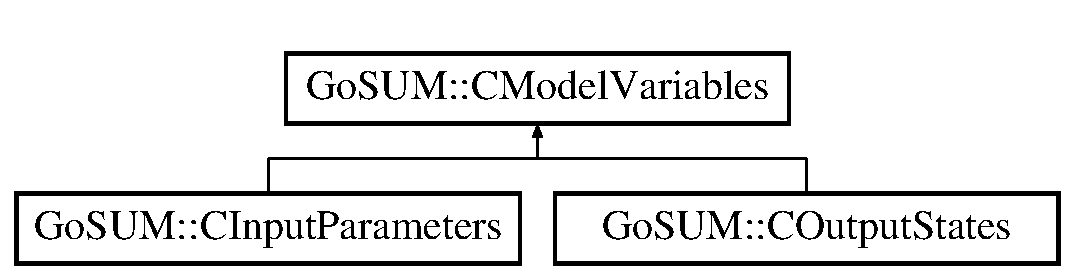
\includegraphics[height=2.000000cm]{class_go_s_u_m_1_1_c_model_variables}
\end{center}
\end{figure}
\subsection*{Public Member Functions}
\begin{DoxyCompactItemize}
\item 
\hyperlink{class_go_s_u_m_1_1_c_model_variables_a539072552d0e09d02843a1fa44b11d3b}{C\-Model\-Variables} ()
\item 
virtual \hyperlink{class_go_s_u_m_1_1_c_model_variables_a441352009e92c8d767e798d41e9c19ea}{$\sim$\-C\-Model\-Variables} ()
\item 
std\-::string \hyperlink{class_go_s_u_m_1_1_c_model_variables_a9351f5510881471981abd458b4ca4488}{base\-Name} () const 
\begin{DoxyCompactList}\small\item\em Returns base name. \end{DoxyCompactList}\item 
void \hyperlink{class_go_s_u_m_1_1_c_model_variables_a11a9ee018a817a9d6ce0914e6bed0b91}{set\-Base\-Name} (std\-::string \-\_\-basename)
\begin{DoxyCompactList}\small\item\em Sets base name. \end{DoxyCompactList}\item 
std\-::string \hyperlink{class_go_s_u_m_1_1_c_model_variables_af11771a78369e73163d30e13e6e90c2f}{next\-Name} () const 
\begin{DoxyCompactList}\small\item\em Returns next variable name. \end{DoxyCompactList}\item 
bool \hyperlink{class_go_s_u_m_1_1_c_model_variables_a89540611f83890ddefa97505ef2c02de}{empty} () const 
\begin{DoxyCompactList}\small\item\em Returns true if object contains no model variables, false otherwise. \end{DoxyCompactList}\item 
bool \hyperlink{class_go_s_u_m_1_1_c_model_variables_aed850606b33ac1a1d04293eb49ea34fa}{empty\-Samples} () const 
\begin{DoxyCompactList}\small\item\em Returns true if object contains no samples, false otherwise. \end{DoxyCompactList}\item 
void \hyperlink{class_go_s_u_m_1_1_c_model_variables_aae62db449aed7eaeb8eefb0143e5de2c}{clear} ()
\item 
void \hyperlink{class_go_s_u_m_1_1_c_model_variables_a5a7a04ad12b2d23d0921cded3d7121de}{clear\-Samples} ()
\begin{DoxyCompactList}\small\item\em Clears data. \end{DoxyCompactList}\item 
const \hyperlink{class_go_s_u_m_1_1_c_model_variable}{C\-Model\-Variable} \& \hyperlink{class_go_s_u_m_1_1_c_model_variables_af311763812d7724409678b8fc87f237c}{operator()} (int \-\_\-at) const 
\begin{DoxyCompactList}\small\item\em Clears samples. \end{DoxyCompactList}\item 
\hyperlink{class_go_s_u_m_1_1_c_model_variable}{C\-Model\-Variable} \& \hyperlink{class_go_s_u_m_1_1_c_model_variables_a08d7808b67e19ba1f97603901f80cff9}{operator()} (int \-\_\-at)
\begin{DoxyCompactList}\small\item\em Returns paticular model variable. \end{DoxyCompactList}\item 
int \hyperlink{class_go_s_u_m_1_1_c_model_variables_ac78a93b9814e6b053f3cd7d72ccfa794}{find} (const std\-::string \&\-\_\-name) const 
\begin{DoxyCompactList}\small\item\em $<$ Finds model variable by name, returns it's index. \end{DoxyCompactList}\item 
int \hyperlink{class_go_s_u_m_1_1_c_model_variables_a3c9ed3cad5fd7c1773a2b13d2e0d4cbe}{size} () const 
\begin{DoxyCompactList}\small\item\em Returns the size of model variables. \end{DoxyCompactList}\item 
int \hyperlink{class_go_s_u_m_1_1_c_model_variables_a0fb75174963bd1a9ce6f6969c5bc57ab}{expanded\-Size} () const 
\begin{DoxyCompactList}\small\item\em Returns expanded size of model variables (due to categorical). \end{DoxyCompactList}\item 
int \hyperlink{class_go_s_u_m_1_1_c_model_variables_aaa7564978d3d08d4f9ab0a3c58f59239}{sample\-Size} () const 
\begin{DoxyCompactList}\small\item\em Returns sample size. \end{DoxyCompactList}\item 
\hyperlink{class_go_s_u_m_1_1_c_model_variable}{C\-Model\-Variable} $\ast$ \hyperlink{class_go_s_u_m_1_1_c_model_variables_a5c03df35b287bec6b42dfb1b13a8c7cc}{add} (\hyperlink{class_go_s_u_m_1_1_c_model_variable}{C\-Model\-Variable} $\ast$\-\_\-p\-M\-V)
\begin{DoxyCompactList}\small\item\em Adds, i.\-e. pushes back model variable. \end{DoxyCompactList}\item 
\hyperlink{class_go_s_u_m_1_1_c_model_variable}{C\-Model\-Variable} $\ast$ \hyperlink{class_go_s_u_m_1_1_c_model_variables_aaf419a53e0a053f11801718b7228c578}{insert} (\hyperlink{class_go_s_u_m_1_1_c_model_variable}{C\-Model\-Variable} $\ast$\-\_\-p\-M\-V, int \-\_\-before)
\item 
void \hyperlink{class_go_s_u_m_1_1_c_model_variables_a915503ed71fab8f50e6fa05a13eb9aba}{erase} (int \-\_\-at)
\item 
\hyperlink{class_go_s_u_m_1_1_c_model_variable}{C\-Model\-Variable} $\ast$ \hyperlink{class_go_s_u_m_1_1_c_model_variables_afe392d83fccb9fdf63edbd80e532cf31}{replace} (int \-\_\-at, \hyperlink{class_go_s_u_m_1_1_c_model_variable}{C\-Model\-Variable} $\ast$\-\_\-p\-M\-V)
\item 
void \hyperlink{class_go_s_u_m_1_1_c_model_variables_a2489a0422fc411d13f266bf24639a41c}{rename} (int \-\_\-at, const std\-::string \&\-\_\-name)
\item 
std\-::vector$<$ Array\-Xd $>$ \hyperlink{class_go_s_u_m_1_1_c_model_variables_ab2ae6e3a54d10b6d90f98f402a89f6ee}{samples} ()
\begin{DoxyCompactList}\small\item\em Returns all samples. \end{DoxyCompactList}\item 
void \hyperlink{class_go_s_u_m_1_1_c_model_variables_a7f8df103f73331f3bca77b1baf13da0b}{set\-Samples} (const std\-::vector$<$ Array\-Xd $>$ \&\-\_\-samples)
\begin{DoxyCompactList}\small\item\em Sets samples of all model variables to values in \-\_\-samples. \end{DoxyCompactList}\item 
void \hyperlink{class_go_s_u_m_1_1_c_model_variables_afaf27c06a9addbf93646c67360d3eb48}{compute\-Statistics} (int \-\_\-n)
\begin{DoxyCompactList}\small\item\em Computes statistics of all model variables. \end{DoxyCompactList}\item 
void \hyperlink{class_go_s_u_m_1_1_c_model_variables_a4e7df5a62ff6c0eda6f0de196a704e12}{compute\-Statistics} (const std\-::vector$<$ int $>$ \&\-\_\-selected, int \-\_\-n)
\item 
void \hyperlink{class_go_s_u_m_1_1_c_model_variables_a8b7087357a18fbfaba390a47ce3ba309}{set\-Distributions} (const std\-::vector$<$ int $>$ \&\-\_\-selected)
\begin{DoxyCompactList}\small\item\em For selected model variables detects distribution from empirical sample data. \end{DoxyCompactList}\item 
void \hyperlink{class_go_s_u_m_1_1_c_model_variables_a8c5d6852c04dc7d5dcfdf49cdbb801a1}{set\-Distributions} ()
\begin{DoxyCompactList}\small\item\em For all model variables detects distribution from empirical sample data. \end{DoxyCompactList}\item 
void \hyperlink{class_go_s_u_m_1_1_c_model_variables_a75268d82c04c54ca4496ff5e1b1406ee}{set\-N\-Tuple} (const Array\-Xd \&X, int \-\_\-at)
\begin{DoxyCompactList}\small\item\em Sets \-\_\-at sample values of all model variables. \end{DoxyCompactList}\item 
Array\-Xd \hyperlink{class_go_s_u_m_1_1_c_model_variables_a92bd5ab6d1d46551a415a98541a2d32a}{n\-Tuple} (int \-\_\-at) const 
\begin{DoxyCompactList}\small\item\em Returns n-\/tuple containing \-\_\-at sample values of all model variables. \end{DoxyCompactList}\item 
Array\-Xd \hyperlink{class_go_s_u_m_1_1_c_model_variables_a8aca475f569e0e81bf88d697468cdf67}{expanded\-N\-Tuple} (int \-\_\-at) const 
\begin{DoxyCompactList}\small\item\em Returns expanded n-\/tuple containing \-\_\-at sample values of all model variables. \end{DoxyCompactList}\item 
Array\-Xd \hyperlink{class_go_s_u_m_1_1_c_model_variables_ad6d83d056cb740499c710711f3fcff1d}{expand\-N\-Tuple} (const Array\-Xd \&X) const 
\begin{DoxyCompactList}\small\item\em Expands given n-\/tuple. \end{DoxyCompactList}\item 
void \hyperlink{class_go_s_u_m_1_1_c_model_variables_a28359235bd83070fa2c40bdeeb90fe01}{set\-Normalization} ()
\item 
double \hyperlink{class_go_s_u_m_1_1_c_model_variables_abf4db473db4a17e0010cae650aa0d907}{normalize} (double Vi, int i) const 
\begin{DoxyCompactList}\small\item\em (Re)sets normalization of model variables using empirical data in samples. \end{DoxyCompactList}\item 
Array\-Xd \hyperlink{class_go_s_u_m_1_1_c_model_variables_ac2bbbbc99a0717ab9d5d501b0cf86427}{normalize} (const Array\-Xd \&V) const 
\begin{DoxyCompactList}\small\item\em Normalizes values of all (expanded) model variables. \end{DoxyCompactList}\item 
double \hyperlink{class_go_s_u_m_1_1_c_model_variables_a42b21bbfdd60a640f0925802035bd772}{denormalize} (double Vi, int i) const 
\begin{DoxyCompactList}\small\item\em Denoramlizes value of the ith (expanded) model variable. \end{DoxyCompactList}\item 
Array\-Xd \hyperlink{class_go_s_u_m_1_1_c_model_variables_aefcc9a87015565230d6f8dd0897173bd}{denormalize} (const Array\-Xd \&V) const 
\begin{DoxyCompactList}\small\item\em Denormalizes values of all (expanded) model variables. \end{DoxyCompactList}\item 
double \hyperlink{class_go_s_u_m_1_1_c_model_variables_a3e372277479386d4ed795b718296b439}{d\-Normalize} (int i) const 
\begin{DoxyCompactList}\small\item\em Returns derivative of the normalization function for ith (expanded) model variable. \end{DoxyCompactList}\item 
Array\-Xd \hyperlink{class_go_s_u_m_1_1_c_model_variables_a1a029447ceb9c51a71bd22ccf4a01802}{d\-Normalize} () const 
\begin{DoxyCompactList}\small\item\em Returns derivatives of the normalization function for (expanded) model variables. \end{DoxyCompactList}\item 
double \hyperlink{class_go_s_u_m_1_1_c_model_variables_abc720f34bfd0c1044150675d5cd5594d}{d\-Denormalize} (int i) const 
\begin{DoxyCompactList}\small\item\em Returns derivative of the denormalization function for ith (expanded) model variable. \end{DoxyCompactList}\item 
Array\-Xd \hyperlink{class_go_s_u_m_1_1_c_model_variables_a65b28acfc2b82e889679abf55b94c2c1}{d\-Denormalize} () const 
\begin{DoxyCompactList}\small\item\em Returns derivatives of the denormalization function for (expanded) model variables. \end{DoxyCompactList}\item 
Array\-Xd \hyperlink{class_go_s_u_m_1_1_c_model_variables_a43186a53e67e1cfd7f0115977bac1c17}{hc\-Point2\-Model\-Point} (const Array\-Xd \&x)
\begin{DoxyCompactList}\small\item\em Maps hypercube point to model point. \end{DoxyCompactList}\item 
void \hyperlink{class_go_s_u_m_1_1_c_model_variables_a96c11c4fd04abebab9e981d3bdf3db11}{erase\-Selected\-Samples} (const std\-::vector$<$ int $>$ \&sel)
\end{DoxyCompactItemize}
\subsection*{Protected Member Functions}
\begin{DoxyCompactItemize}
\item 
{\footnotesize template$<$class Archive $>$ }\\void \hyperlink{class_go_s_u_m_1_1_c_model_variables_aa2274914e5ce27be8925b5894b425fa3}{serialize} (Archive \&ar, const unsigned int version)
\end{DoxyCompactItemize}
\subsection*{Static Protected Member Functions}
\begin{DoxyCompactItemize}
\item 
static bool \hyperlink{class_go_s_u_m_1_1_c_model_variables_ae9f6f163a086ba7c964ff8cf85a6cfb4}{is\-Model\-Variable\-Name} (const \hyperlink{class_go_s_u_m_1_1_c_model_variable}{C\-Model\-Variable} \&\-\_\-a\-M\-V)
\begin{DoxyCompactList}\small\item\em Used in member function Find. \end{DoxyCompactList}\end{DoxyCompactItemize}
\subsection*{Protected Attributes}
\begin{DoxyCompactItemize}
\item 
std\-::string \hyperlink{class_go_s_u_m_1_1_c_model_variables_a3e0a177e926f2512b4499a47ecc9c957}{basename}
\begin{DoxyCompactList}\small\item\em Holds basename used for generating model variable unique names. \end{DoxyCompactList}\item 
boost\-::ptr\-\_\-vector$<$ \hyperlink{class_go_s_u_m_1_1_c_model_variable}{C\-Model\-Variable} $>$ \hyperlink{class_go_s_u_m_1_1_c_model_variables_a9ce0daf443666eb920bbbbdee00e1e37}{mvs}
\begin{DoxyCompactList}\small\item\em Holds pointers to model variables. \end{DoxyCompactList}\item 
Array\-Xd \hyperlink{class_go_s_u_m_1_1_c_model_variables_a44c359c9aeda8913e9c93bdf133638dd}{trn}
\item 
Array\-Xd \hyperlink{class_go_s_u_m_1_1_c_model_variables_a82725532f90f4b4c6c6bd6b4c25d20c3}{scl}
\end{DoxyCompactItemize}
\subsection*{Static Protected Attributes}
\begin{DoxyCompactItemize}
\item 
static std\-::string \hyperlink{class_go_s_u_m_1_1_c_model_variables_aa295a3899598dab50afc56434eb7ace4}{name\-To\-Find} = \char`\"{}\char`\"{}
\begin{DoxyCompactList}\small\item\em Used in member function Find. \end{DoxyCompactList}\end{DoxyCompactItemize}
\subsection*{Friends}
\begin{DoxyCompactItemize}
\item 
class \hyperlink{class_go_s_u_m_1_1_c_model_variables_ac98d07dd8f7b70e16ccb9a01abf56b9c}{boost\-::serialization\-::access}
\begin{DoxyCompactList}\small\item\em Boost serialization. \end{DoxyCompactList}\end{DoxyCompactItemize}


\subsection{Detailed Description}
Class for the vector of model variables (inputs \& outputs). 

\subsection{Constructor \& Destructor Documentation}
\hypertarget{class_go_s_u_m_1_1_c_model_variables_a539072552d0e09d02843a1fa44b11d3b}{\index{Go\-S\-U\-M\-::\-C\-Model\-Variables@{Go\-S\-U\-M\-::\-C\-Model\-Variables}!C\-Model\-Variables@{C\-Model\-Variables}}
\index{C\-Model\-Variables@{C\-Model\-Variables}!GoSUM::CModelVariables@{Go\-S\-U\-M\-::\-C\-Model\-Variables}}
\subsubsection[{C\-Model\-Variables}]{\setlength{\rightskip}{0pt plus 5cm}Go\-S\-U\-M\-::\-C\-Model\-Variables\-::\-C\-Model\-Variables (
\begin{DoxyParamCaption}
{}
\end{DoxyParamCaption}
)\hspace{0.3cm}{\ttfamily [inline]}}}\label{class_go_s_u_m_1_1_c_model_variables_a539072552d0e09d02843a1fa44b11d3b}
\hypertarget{class_go_s_u_m_1_1_c_model_variables_a441352009e92c8d767e798d41e9c19ea}{\index{Go\-S\-U\-M\-::\-C\-Model\-Variables@{Go\-S\-U\-M\-::\-C\-Model\-Variables}!$\sim$\-C\-Model\-Variables@{$\sim$\-C\-Model\-Variables}}
\index{$\sim$\-C\-Model\-Variables@{$\sim$\-C\-Model\-Variables}!GoSUM::CModelVariables@{Go\-S\-U\-M\-::\-C\-Model\-Variables}}
\subsubsection[{$\sim$\-C\-Model\-Variables}]{\setlength{\rightskip}{0pt plus 5cm}virtual Go\-S\-U\-M\-::\-C\-Model\-Variables\-::$\sim$\-C\-Model\-Variables (
\begin{DoxyParamCaption}
{}
\end{DoxyParamCaption}
)\hspace{0.3cm}{\ttfamily [inline]}, {\ttfamily [virtual]}}}\label{class_go_s_u_m_1_1_c_model_variables_a441352009e92c8d767e798d41e9c19ea}


\subsection{Member Function Documentation}
\hypertarget{class_go_s_u_m_1_1_c_model_variables_a5c03df35b287bec6b42dfb1b13a8c7cc}{\index{Go\-S\-U\-M\-::\-C\-Model\-Variables@{Go\-S\-U\-M\-::\-C\-Model\-Variables}!add@{add}}
\index{add@{add}!GoSUM::CModelVariables@{Go\-S\-U\-M\-::\-C\-Model\-Variables}}
\subsubsection[{add}]{\setlength{\rightskip}{0pt plus 5cm}{\bf C\-Model\-Variable}$\ast$ Go\-S\-U\-M\-::\-C\-Model\-Variables\-::add (
\begin{DoxyParamCaption}
\item[{{\bf C\-Model\-Variable} $\ast$}]{\-\_\-p\-M\-V}
\end{DoxyParamCaption}
)\hspace{0.3cm}{\ttfamily [inline]}}}\label{class_go_s_u_m_1_1_c_model_variables_a5c03df35b287bec6b42dfb1b13a8c7cc}


Adds, i.\-e. pushes back model variable. 

\hypertarget{class_go_s_u_m_1_1_c_model_variables_a9351f5510881471981abd458b4ca4488}{\index{Go\-S\-U\-M\-::\-C\-Model\-Variables@{Go\-S\-U\-M\-::\-C\-Model\-Variables}!base\-Name@{base\-Name}}
\index{base\-Name@{base\-Name}!GoSUM::CModelVariables@{Go\-S\-U\-M\-::\-C\-Model\-Variables}}
\subsubsection[{base\-Name}]{\setlength{\rightskip}{0pt plus 5cm}std\-::string Go\-S\-U\-M\-::\-C\-Model\-Variables\-::base\-Name (
\begin{DoxyParamCaption}
{}
\end{DoxyParamCaption}
) const\hspace{0.3cm}{\ttfamily [inline]}}}\label{class_go_s_u_m_1_1_c_model_variables_a9351f5510881471981abd458b4ca4488}


Returns base name. 

\hypertarget{class_go_s_u_m_1_1_c_model_variables_aae62db449aed7eaeb8eefb0143e5de2c}{\index{Go\-S\-U\-M\-::\-C\-Model\-Variables@{Go\-S\-U\-M\-::\-C\-Model\-Variables}!clear@{clear}}
\index{clear@{clear}!GoSUM::CModelVariables@{Go\-S\-U\-M\-::\-C\-Model\-Variables}}
\subsubsection[{clear}]{\setlength{\rightskip}{0pt plus 5cm}void Go\-S\-U\-M\-::\-C\-Model\-Variables\-::clear (
\begin{DoxyParamCaption}
{}
\end{DoxyParamCaption}
)\hspace{0.3cm}{\ttfamily [inline]}}}\label{class_go_s_u_m_1_1_c_model_variables_aae62db449aed7eaeb8eefb0143e5de2c}
\hypertarget{class_go_s_u_m_1_1_c_model_variables_a5a7a04ad12b2d23d0921cded3d7121de}{\index{Go\-S\-U\-M\-::\-C\-Model\-Variables@{Go\-S\-U\-M\-::\-C\-Model\-Variables}!clear\-Samples@{clear\-Samples}}
\index{clear\-Samples@{clear\-Samples}!GoSUM::CModelVariables@{Go\-S\-U\-M\-::\-C\-Model\-Variables}}
\subsubsection[{clear\-Samples}]{\setlength{\rightskip}{0pt plus 5cm}void Go\-S\-U\-M\-::\-C\-Model\-Variables\-::clear\-Samples (
\begin{DoxyParamCaption}
{}
\end{DoxyParamCaption}
)\hspace{0.3cm}{\ttfamily [inline]}}}\label{class_go_s_u_m_1_1_c_model_variables_a5a7a04ad12b2d23d0921cded3d7121de}


Clears data. 

\hypertarget{class_go_s_u_m_1_1_c_model_variables_afaf27c06a9addbf93646c67360d3eb48}{\index{Go\-S\-U\-M\-::\-C\-Model\-Variables@{Go\-S\-U\-M\-::\-C\-Model\-Variables}!compute\-Statistics@{compute\-Statistics}}
\index{compute\-Statistics@{compute\-Statistics}!GoSUM::CModelVariables@{Go\-S\-U\-M\-::\-C\-Model\-Variables}}
\subsubsection[{compute\-Statistics}]{\setlength{\rightskip}{0pt plus 5cm}void Go\-S\-U\-M\-::\-C\-Model\-Variables\-::compute\-Statistics (
\begin{DoxyParamCaption}
\item[{int}]{\-\_\-n}
\end{DoxyParamCaption}
)\hspace{0.3cm}{\ttfamily [inline]}}}\label{class_go_s_u_m_1_1_c_model_variables_afaf27c06a9addbf93646c67360d3eb48}


Computes statistics of all model variables. 

\hypertarget{class_go_s_u_m_1_1_c_model_variables_a4e7df5a62ff6c0eda6f0de196a704e12}{\index{Go\-S\-U\-M\-::\-C\-Model\-Variables@{Go\-S\-U\-M\-::\-C\-Model\-Variables}!compute\-Statistics@{compute\-Statistics}}
\index{compute\-Statistics@{compute\-Statistics}!GoSUM::CModelVariables@{Go\-S\-U\-M\-::\-C\-Model\-Variables}}
\subsubsection[{compute\-Statistics}]{\setlength{\rightskip}{0pt plus 5cm}void Go\-S\-U\-M\-::\-C\-Model\-Variables\-::compute\-Statistics (
\begin{DoxyParamCaption}
\item[{const std\-::vector$<$ int $>$ \&}]{\-\_\-selected, }
\item[{int}]{\-\_\-n}
\end{DoxyParamCaption}
)\hspace{0.3cm}{\ttfamily [inline]}}}\label{class_go_s_u_m_1_1_c_model_variables_a4e7df5a62ff6c0eda6f0de196a704e12}

\begin{DoxyParams}{Parameters}
{\em \-\_\-n} & Computes statistics of selected model variables. \\
\hline
\end{DoxyParams}
\hypertarget{class_go_s_u_m_1_1_c_model_variables_abc720f34bfd0c1044150675d5cd5594d}{\index{Go\-S\-U\-M\-::\-C\-Model\-Variables@{Go\-S\-U\-M\-::\-C\-Model\-Variables}!d\-Denormalize@{d\-Denormalize}}
\index{d\-Denormalize@{d\-Denormalize}!GoSUM::CModelVariables@{Go\-S\-U\-M\-::\-C\-Model\-Variables}}
\subsubsection[{d\-Denormalize}]{\setlength{\rightskip}{0pt plus 5cm}double Go\-S\-U\-M\-::\-C\-Model\-Variables\-::d\-Denormalize (
\begin{DoxyParamCaption}
\item[{int}]{i}
\end{DoxyParamCaption}
) const\hspace{0.3cm}{\ttfamily [inline]}}}\label{class_go_s_u_m_1_1_c_model_variables_abc720f34bfd0c1044150675d5cd5594d}


Returns derivative of the denormalization function for ith (expanded) model variable. 

\hypertarget{class_go_s_u_m_1_1_c_model_variables_a65b28acfc2b82e889679abf55b94c2c1}{\index{Go\-S\-U\-M\-::\-C\-Model\-Variables@{Go\-S\-U\-M\-::\-C\-Model\-Variables}!d\-Denormalize@{d\-Denormalize}}
\index{d\-Denormalize@{d\-Denormalize}!GoSUM::CModelVariables@{Go\-S\-U\-M\-::\-C\-Model\-Variables}}
\subsubsection[{d\-Denormalize}]{\setlength{\rightskip}{0pt plus 5cm}Array\-Xd Go\-S\-U\-M\-::\-C\-Model\-Variables\-::d\-Denormalize (
\begin{DoxyParamCaption}
{}
\end{DoxyParamCaption}
) const\hspace{0.3cm}{\ttfamily [inline]}}}\label{class_go_s_u_m_1_1_c_model_variables_a65b28acfc2b82e889679abf55b94c2c1}


Returns derivatives of the denormalization function for (expanded) model variables. 

\hypertarget{class_go_s_u_m_1_1_c_model_variables_a42b21bbfdd60a640f0925802035bd772}{\index{Go\-S\-U\-M\-::\-C\-Model\-Variables@{Go\-S\-U\-M\-::\-C\-Model\-Variables}!denormalize@{denormalize}}
\index{denormalize@{denormalize}!GoSUM::CModelVariables@{Go\-S\-U\-M\-::\-C\-Model\-Variables}}
\subsubsection[{denormalize}]{\setlength{\rightskip}{0pt plus 5cm}double Go\-S\-U\-M\-::\-C\-Model\-Variables\-::denormalize (
\begin{DoxyParamCaption}
\item[{double}]{Vi, }
\item[{int}]{i}
\end{DoxyParamCaption}
) const\hspace{0.3cm}{\ttfamily [inline]}}}\label{class_go_s_u_m_1_1_c_model_variables_a42b21bbfdd60a640f0925802035bd772}


Denoramlizes value of the ith (expanded) model variable. 

\hypertarget{class_go_s_u_m_1_1_c_model_variables_aefcc9a87015565230d6f8dd0897173bd}{\index{Go\-S\-U\-M\-::\-C\-Model\-Variables@{Go\-S\-U\-M\-::\-C\-Model\-Variables}!denormalize@{denormalize}}
\index{denormalize@{denormalize}!GoSUM::CModelVariables@{Go\-S\-U\-M\-::\-C\-Model\-Variables}}
\subsubsection[{denormalize}]{\setlength{\rightskip}{0pt plus 5cm}Array\-Xd Go\-S\-U\-M\-::\-C\-Model\-Variables\-::denormalize (
\begin{DoxyParamCaption}
\item[{const Array\-Xd \&}]{V}
\end{DoxyParamCaption}
) const\hspace{0.3cm}{\ttfamily [inline]}}}\label{class_go_s_u_m_1_1_c_model_variables_aefcc9a87015565230d6f8dd0897173bd}


Denormalizes values of all (expanded) model variables. 

\hypertarget{class_go_s_u_m_1_1_c_model_variables_a3e372277479386d4ed795b718296b439}{\index{Go\-S\-U\-M\-::\-C\-Model\-Variables@{Go\-S\-U\-M\-::\-C\-Model\-Variables}!d\-Normalize@{d\-Normalize}}
\index{d\-Normalize@{d\-Normalize}!GoSUM::CModelVariables@{Go\-S\-U\-M\-::\-C\-Model\-Variables}}
\subsubsection[{d\-Normalize}]{\setlength{\rightskip}{0pt plus 5cm}double Go\-S\-U\-M\-::\-C\-Model\-Variables\-::d\-Normalize (
\begin{DoxyParamCaption}
\item[{int}]{i}
\end{DoxyParamCaption}
) const\hspace{0.3cm}{\ttfamily [inline]}}}\label{class_go_s_u_m_1_1_c_model_variables_a3e372277479386d4ed795b718296b439}


Returns derivative of the normalization function for ith (expanded) model variable. 

\hypertarget{class_go_s_u_m_1_1_c_model_variables_a1a029447ceb9c51a71bd22ccf4a01802}{\index{Go\-S\-U\-M\-::\-C\-Model\-Variables@{Go\-S\-U\-M\-::\-C\-Model\-Variables}!d\-Normalize@{d\-Normalize}}
\index{d\-Normalize@{d\-Normalize}!GoSUM::CModelVariables@{Go\-S\-U\-M\-::\-C\-Model\-Variables}}
\subsubsection[{d\-Normalize}]{\setlength{\rightskip}{0pt plus 5cm}Array\-Xd Go\-S\-U\-M\-::\-C\-Model\-Variables\-::d\-Normalize (
\begin{DoxyParamCaption}
{}
\end{DoxyParamCaption}
) const\hspace{0.3cm}{\ttfamily [inline]}}}\label{class_go_s_u_m_1_1_c_model_variables_a1a029447ceb9c51a71bd22ccf4a01802}


Returns derivatives of the normalization function for (expanded) model variables. 

\hypertarget{class_go_s_u_m_1_1_c_model_variables_a89540611f83890ddefa97505ef2c02de}{\index{Go\-S\-U\-M\-::\-C\-Model\-Variables@{Go\-S\-U\-M\-::\-C\-Model\-Variables}!empty@{empty}}
\index{empty@{empty}!GoSUM::CModelVariables@{Go\-S\-U\-M\-::\-C\-Model\-Variables}}
\subsubsection[{empty}]{\setlength{\rightskip}{0pt plus 5cm}bool Go\-S\-U\-M\-::\-C\-Model\-Variables\-::empty (
\begin{DoxyParamCaption}
{}
\end{DoxyParamCaption}
) const\hspace{0.3cm}{\ttfamily [inline]}}}\label{class_go_s_u_m_1_1_c_model_variables_a89540611f83890ddefa97505ef2c02de}


Returns true if object contains no model variables, false otherwise. 

\hypertarget{class_go_s_u_m_1_1_c_model_variables_aed850606b33ac1a1d04293eb49ea34fa}{\index{Go\-S\-U\-M\-::\-C\-Model\-Variables@{Go\-S\-U\-M\-::\-C\-Model\-Variables}!empty\-Samples@{empty\-Samples}}
\index{empty\-Samples@{empty\-Samples}!GoSUM::CModelVariables@{Go\-S\-U\-M\-::\-C\-Model\-Variables}}
\subsubsection[{empty\-Samples}]{\setlength{\rightskip}{0pt plus 5cm}bool Go\-S\-U\-M\-::\-C\-Model\-Variables\-::empty\-Samples (
\begin{DoxyParamCaption}
{}
\end{DoxyParamCaption}
) const\hspace{0.3cm}{\ttfamily [inline]}}}\label{class_go_s_u_m_1_1_c_model_variables_aed850606b33ac1a1d04293eb49ea34fa}


Returns true if object contains no samples, false otherwise. 

\hypertarget{class_go_s_u_m_1_1_c_model_variables_a915503ed71fab8f50e6fa05a13eb9aba}{\index{Go\-S\-U\-M\-::\-C\-Model\-Variables@{Go\-S\-U\-M\-::\-C\-Model\-Variables}!erase@{erase}}
\index{erase@{erase}!GoSUM::CModelVariables@{Go\-S\-U\-M\-::\-C\-Model\-Variables}}
\subsubsection[{erase}]{\setlength{\rightskip}{0pt plus 5cm}void Go\-S\-U\-M\-::\-C\-Model\-Variables\-::erase (
\begin{DoxyParamCaption}
\item[{int}]{\-\_\-at}
\end{DoxyParamCaption}
)\hspace{0.3cm}{\ttfamily [inline]}}}\label{class_go_s_u_m_1_1_c_model_variables_a915503ed71fab8f50e6fa05a13eb9aba}

\begin{DoxyParams}{Parameters}
{\em \-\_\-at} & Erases particular model variable. \\
\hline
\end{DoxyParams}
\hypertarget{class_go_s_u_m_1_1_c_model_variables_a96c11c4fd04abebab9e981d3bdf3db11}{\index{Go\-S\-U\-M\-::\-C\-Model\-Variables@{Go\-S\-U\-M\-::\-C\-Model\-Variables}!erase\-Selected\-Samples@{erase\-Selected\-Samples}}
\index{erase\-Selected\-Samples@{erase\-Selected\-Samples}!GoSUM::CModelVariables@{Go\-S\-U\-M\-::\-C\-Model\-Variables}}
\subsubsection[{erase\-Selected\-Samples}]{\setlength{\rightskip}{0pt plus 5cm}void Go\-S\-U\-M\-::\-C\-Model\-Variables\-::erase\-Selected\-Samples (
\begin{DoxyParamCaption}
\item[{const std\-::vector$<$ int $>$ \&}]{sel}
\end{DoxyParamCaption}
)\hspace{0.3cm}{\ttfamily [inline]}}}\label{class_go_s_u_m_1_1_c_model_variables_a96c11c4fd04abebab9e981d3bdf3db11}

\begin{DoxyParams}{Parameters}
{\em sel} & Erases selected sample values. \\
\hline
\end{DoxyParams}
\hypertarget{class_go_s_u_m_1_1_c_model_variables_a8aca475f569e0e81bf88d697468cdf67}{\index{Go\-S\-U\-M\-::\-C\-Model\-Variables@{Go\-S\-U\-M\-::\-C\-Model\-Variables}!expanded\-N\-Tuple@{expanded\-N\-Tuple}}
\index{expanded\-N\-Tuple@{expanded\-N\-Tuple}!GoSUM::CModelVariables@{Go\-S\-U\-M\-::\-C\-Model\-Variables}}
\subsubsection[{expanded\-N\-Tuple}]{\setlength{\rightskip}{0pt plus 5cm}Array\-Xd Go\-S\-U\-M\-::\-C\-Model\-Variables\-::expanded\-N\-Tuple (
\begin{DoxyParamCaption}
\item[{int}]{\-\_\-at}
\end{DoxyParamCaption}
) const}}\label{class_go_s_u_m_1_1_c_model_variables_a8aca475f569e0e81bf88d697468cdf67}


Returns expanded n-\/tuple containing \-\_\-at sample values of all model variables. 

\hypertarget{class_go_s_u_m_1_1_c_model_variables_a0fb75174963bd1a9ce6f6969c5bc57ab}{\index{Go\-S\-U\-M\-::\-C\-Model\-Variables@{Go\-S\-U\-M\-::\-C\-Model\-Variables}!expanded\-Size@{expanded\-Size}}
\index{expanded\-Size@{expanded\-Size}!GoSUM::CModelVariables@{Go\-S\-U\-M\-::\-C\-Model\-Variables}}
\subsubsection[{expanded\-Size}]{\setlength{\rightskip}{0pt plus 5cm}int Go\-S\-U\-M\-::\-C\-Model\-Variables\-::expanded\-Size (
\begin{DoxyParamCaption}
{}
\end{DoxyParamCaption}
) const}}\label{class_go_s_u_m_1_1_c_model_variables_a0fb75174963bd1a9ce6f6969c5bc57ab}


Returns expanded size of model variables (due to categorical). 

\hypertarget{class_go_s_u_m_1_1_c_model_variables_ad6d83d056cb740499c710711f3fcff1d}{\index{Go\-S\-U\-M\-::\-C\-Model\-Variables@{Go\-S\-U\-M\-::\-C\-Model\-Variables}!expand\-N\-Tuple@{expand\-N\-Tuple}}
\index{expand\-N\-Tuple@{expand\-N\-Tuple}!GoSUM::CModelVariables@{Go\-S\-U\-M\-::\-C\-Model\-Variables}}
\subsubsection[{expand\-N\-Tuple}]{\setlength{\rightskip}{0pt plus 5cm}Array\-Xd Go\-S\-U\-M\-::\-C\-Model\-Variables\-::expand\-N\-Tuple (
\begin{DoxyParamCaption}
\item[{const Array\-Xd \&}]{X}
\end{DoxyParamCaption}
) const}}\label{class_go_s_u_m_1_1_c_model_variables_ad6d83d056cb740499c710711f3fcff1d}


Expands given n-\/tuple. 

\hypertarget{class_go_s_u_m_1_1_c_model_variables_ac78a93b9814e6b053f3cd7d72ccfa794}{\index{Go\-S\-U\-M\-::\-C\-Model\-Variables@{Go\-S\-U\-M\-::\-C\-Model\-Variables}!find@{find}}
\index{find@{find}!GoSUM::CModelVariables@{Go\-S\-U\-M\-::\-C\-Model\-Variables}}
\subsubsection[{find}]{\setlength{\rightskip}{0pt plus 5cm}int Go\-S\-U\-M\-::\-C\-Model\-Variables\-::find (
\begin{DoxyParamCaption}
\item[{const std\-::string \&}]{\-\_\-name}
\end{DoxyParamCaption}
) const\hspace{0.3cm}{\ttfamily [inline]}}}\label{class_go_s_u_m_1_1_c_model_variables_ac78a93b9814e6b053f3cd7d72ccfa794}


$<$ Finds model variable by name, returns it's index. 

\hypertarget{class_go_s_u_m_1_1_c_model_variables_a43186a53e67e1cfd7f0115977bac1c17}{\index{Go\-S\-U\-M\-::\-C\-Model\-Variables@{Go\-S\-U\-M\-::\-C\-Model\-Variables}!hc\-Point2\-Model\-Point@{hc\-Point2\-Model\-Point}}
\index{hc\-Point2\-Model\-Point@{hc\-Point2\-Model\-Point}!GoSUM::CModelVariables@{Go\-S\-U\-M\-::\-C\-Model\-Variables}}
\subsubsection[{hc\-Point2\-Model\-Point}]{\setlength{\rightskip}{0pt plus 5cm}Array\-Xd Go\-S\-U\-M\-::\-C\-Model\-Variables\-::hc\-Point2\-Model\-Point (
\begin{DoxyParamCaption}
\item[{const Array\-Xd \&}]{x}
\end{DoxyParamCaption}
)}}\label{class_go_s_u_m_1_1_c_model_variables_a43186a53e67e1cfd7f0115977bac1c17}


Maps hypercube point to model point. 

\hypertarget{class_go_s_u_m_1_1_c_model_variables_aaf419a53e0a053f11801718b7228c578}{\index{Go\-S\-U\-M\-::\-C\-Model\-Variables@{Go\-S\-U\-M\-::\-C\-Model\-Variables}!insert@{insert}}
\index{insert@{insert}!GoSUM::CModelVariables@{Go\-S\-U\-M\-::\-C\-Model\-Variables}}
\subsubsection[{insert}]{\setlength{\rightskip}{0pt plus 5cm}{\bf C\-Model\-Variable}$\ast$ Go\-S\-U\-M\-::\-C\-Model\-Variables\-::insert (
\begin{DoxyParamCaption}
\item[{{\bf C\-Model\-Variable} $\ast$}]{\-\_\-p\-M\-V, }
\item[{int}]{\-\_\-before}
\end{DoxyParamCaption}
)\hspace{0.3cm}{\ttfamily [inline]}}}\label{class_go_s_u_m_1_1_c_model_variables_aaf419a53e0a053f11801718b7228c578}

\begin{DoxyParams}{Parameters}
{\em \-\_\-before} & Inserts model variable in position \-\_\-before. \\
\hline
\end{DoxyParams}
\hypertarget{class_go_s_u_m_1_1_c_model_variables_ae9f6f163a086ba7c964ff8cf85a6cfb4}{\index{Go\-S\-U\-M\-::\-C\-Model\-Variables@{Go\-S\-U\-M\-::\-C\-Model\-Variables}!is\-Model\-Variable\-Name@{is\-Model\-Variable\-Name}}
\index{is\-Model\-Variable\-Name@{is\-Model\-Variable\-Name}!GoSUM::CModelVariables@{Go\-S\-U\-M\-::\-C\-Model\-Variables}}
\subsubsection[{is\-Model\-Variable\-Name}]{\setlength{\rightskip}{0pt plus 5cm}static bool Go\-S\-U\-M\-::\-C\-Model\-Variables\-::is\-Model\-Variable\-Name (
\begin{DoxyParamCaption}
\item[{const {\bf C\-Model\-Variable} \&}]{\-\_\-a\-M\-V}
\end{DoxyParamCaption}
)\hspace{0.3cm}{\ttfamily [inline]}, {\ttfamily [static]}, {\ttfamily [protected]}}}\label{class_go_s_u_m_1_1_c_model_variables_ae9f6f163a086ba7c964ff8cf85a6cfb4}


Used in member function Find. 

\hypertarget{class_go_s_u_m_1_1_c_model_variables_af11771a78369e73163d30e13e6e90c2f}{\index{Go\-S\-U\-M\-::\-C\-Model\-Variables@{Go\-S\-U\-M\-::\-C\-Model\-Variables}!next\-Name@{next\-Name}}
\index{next\-Name@{next\-Name}!GoSUM::CModelVariables@{Go\-S\-U\-M\-::\-C\-Model\-Variables}}
\subsubsection[{next\-Name}]{\setlength{\rightskip}{0pt plus 5cm}std\-::string Go\-S\-U\-M\-::\-C\-Model\-Variables\-::next\-Name (
\begin{DoxyParamCaption}
{}
\end{DoxyParamCaption}
) const}}\label{class_go_s_u_m_1_1_c_model_variables_af11771a78369e73163d30e13e6e90c2f}


Returns next variable name. 

\hypertarget{class_go_s_u_m_1_1_c_model_variables_abf4db473db4a17e0010cae650aa0d907}{\index{Go\-S\-U\-M\-::\-C\-Model\-Variables@{Go\-S\-U\-M\-::\-C\-Model\-Variables}!normalize@{normalize}}
\index{normalize@{normalize}!GoSUM::CModelVariables@{Go\-S\-U\-M\-::\-C\-Model\-Variables}}
\subsubsection[{normalize}]{\setlength{\rightskip}{0pt plus 5cm}double Go\-S\-U\-M\-::\-C\-Model\-Variables\-::normalize (
\begin{DoxyParamCaption}
\item[{double}]{Vi, }
\item[{int}]{i}
\end{DoxyParamCaption}
) const\hspace{0.3cm}{\ttfamily [inline]}}}\label{class_go_s_u_m_1_1_c_model_variables_abf4db473db4a17e0010cae650aa0d907}


(Re)sets normalization of model variables using empirical data in samples. 

Normalizes value of the ith (expanded) model variable. \hypertarget{class_go_s_u_m_1_1_c_model_variables_ac2bbbbc99a0717ab9d5d501b0cf86427}{\index{Go\-S\-U\-M\-::\-C\-Model\-Variables@{Go\-S\-U\-M\-::\-C\-Model\-Variables}!normalize@{normalize}}
\index{normalize@{normalize}!GoSUM::CModelVariables@{Go\-S\-U\-M\-::\-C\-Model\-Variables}}
\subsubsection[{normalize}]{\setlength{\rightskip}{0pt plus 5cm}Array\-Xd Go\-S\-U\-M\-::\-C\-Model\-Variables\-::normalize (
\begin{DoxyParamCaption}
\item[{const Array\-Xd \&}]{V}
\end{DoxyParamCaption}
) const\hspace{0.3cm}{\ttfamily [inline]}}}\label{class_go_s_u_m_1_1_c_model_variables_ac2bbbbc99a0717ab9d5d501b0cf86427}


Normalizes values of all (expanded) model variables. 

\hypertarget{class_go_s_u_m_1_1_c_model_variables_a92bd5ab6d1d46551a415a98541a2d32a}{\index{Go\-S\-U\-M\-::\-C\-Model\-Variables@{Go\-S\-U\-M\-::\-C\-Model\-Variables}!n\-Tuple@{n\-Tuple}}
\index{n\-Tuple@{n\-Tuple}!GoSUM::CModelVariables@{Go\-S\-U\-M\-::\-C\-Model\-Variables}}
\subsubsection[{n\-Tuple}]{\setlength{\rightskip}{0pt plus 5cm}Array\-Xd Go\-S\-U\-M\-::\-C\-Model\-Variables\-::n\-Tuple (
\begin{DoxyParamCaption}
\item[{int}]{\-\_\-at}
\end{DoxyParamCaption}
) const}}\label{class_go_s_u_m_1_1_c_model_variables_a92bd5ab6d1d46551a415a98541a2d32a}


Returns n-\/tuple containing \-\_\-at sample values of all model variables. 

\hypertarget{class_go_s_u_m_1_1_c_model_variables_af311763812d7724409678b8fc87f237c}{\index{Go\-S\-U\-M\-::\-C\-Model\-Variables@{Go\-S\-U\-M\-::\-C\-Model\-Variables}!operator()@{operator()}}
\index{operator()@{operator()}!GoSUM::CModelVariables@{Go\-S\-U\-M\-::\-C\-Model\-Variables}}
\subsubsection[{operator()}]{\setlength{\rightskip}{0pt plus 5cm}const {\bf C\-Model\-Variable}\& Go\-S\-U\-M\-::\-C\-Model\-Variables\-::operator() (
\begin{DoxyParamCaption}
\item[{int}]{\-\_\-at}
\end{DoxyParamCaption}
) const\hspace{0.3cm}{\ttfamily [inline]}}}\label{class_go_s_u_m_1_1_c_model_variables_af311763812d7724409678b8fc87f237c}


Clears samples. 

Returns paticular model variable. \hypertarget{class_go_s_u_m_1_1_c_model_variables_a08d7808b67e19ba1f97603901f80cff9}{\index{Go\-S\-U\-M\-::\-C\-Model\-Variables@{Go\-S\-U\-M\-::\-C\-Model\-Variables}!operator()@{operator()}}
\index{operator()@{operator()}!GoSUM::CModelVariables@{Go\-S\-U\-M\-::\-C\-Model\-Variables}}
\subsubsection[{operator()}]{\setlength{\rightskip}{0pt plus 5cm}{\bf C\-Model\-Variable}\& Go\-S\-U\-M\-::\-C\-Model\-Variables\-::operator() (
\begin{DoxyParamCaption}
\item[{int}]{\-\_\-at}
\end{DoxyParamCaption}
)\hspace{0.3cm}{\ttfamily [inline]}}}\label{class_go_s_u_m_1_1_c_model_variables_a08d7808b67e19ba1f97603901f80cff9}


Returns paticular model variable. 

\hypertarget{class_go_s_u_m_1_1_c_model_variables_a2489a0422fc411d13f266bf24639a41c}{\index{Go\-S\-U\-M\-::\-C\-Model\-Variables@{Go\-S\-U\-M\-::\-C\-Model\-Variables}!rename@{rename}}
\index{rename@{rename}!GoSUM::CModelVariables@{Go\-S\-U\-M\-::\-C\-Model\-Variables}}
\subsubsection[{rename}]{\setlength{\rightskip}{0pt plus 5cm}void Go\-S\-U\-M\-::\-C\-Model\-Variables\-::rename (
\begin{DoxyParamCaption}
\item[{int}]{\-\_\-at, }
\item[{const std\-::string \&}]{\-\_\-name}
\end{DoxyParamCaption}
)\hspace{0.3cm}{\ttfamily [inline]}}}\label{class_go_s_u_m_1_1_c_model_variables_a2489a0422fc411d13f266bf24639a41c}

\begin{DoxyParams}{Parameters}
{\em \-\_\-name} & Renames particular model variable. \\
\hline
\end{DoxyParams}
\hypertarget{class_go_s_u_m_1_1_c_model_variables_afe392d83fccb9fdf63edbd80e532cf31}{\index{Go\-S\-U\-M\-::\-C\-Model\-Variables@{Go\-S\-U\-M\-::\-C\-Model\-Variables}!replace@{replace}}
\index{replace@{replace}!GoSUM::CModelVariables@{Go\-S\-U\-M\-::\-C\-Model\-Variables}}
\subsubsection[{replace}]{\setlength{\rightskip}{0pt plus 5cm}{\bf C\-Model\-Variable}$\ast$ Go\-S\-U\-M\-::\-C\-Model\-Variables\-::replace (
\begin{DoxyParamCaption}
\item[{int}]{\-\_\-at, }
\item[{{\bf C\-Model\-Variable} $\ast$}]{\-\_\-p\-M\-V}
\end{DoxyParamCaption}
)\hspace{0.3cm}{\ttfamily [inline]}}}\label{class_go_s_u_m_1_1_c_model_variables_afe392d83fccb9fdf63edbd80e532cf31}

\begin{DoxyParams}{Parameters}
{\em \-\_\-p\-M\-V} & Replaces model variable in position \-\_\-at with model variable \-\_\-p\-M\-V2. The replaced variable is destroyed. \\
\hline
\end{DoxyParams}
\hypertarget{class_go_s_u_m_1_1_c_model_variables_ab2ae6e3a54d10b6d90f98f402a89f6ee}{\index{Go\-S\-U\-M\-::\-C\-Model\-Variables@{Go\-S\-U\-M\-::\-C\-Model\-Variables}!samples@{samples}}
\index{samples@{samples}!GoSUM::CModelVariables@{Go\-S\-U\-M\-::\-C\-Model\-Variables}}
\subsubsection[{samples}]{\setlength{\rightskip}{0pt plus 5cm}std\-::vector$<$ Array\-Xd $>$ Go\-S\-U\-M\-::\-C\-Model\-Variables\-::samples (
\begin{DoxyParamCaption}
{}
\end{DoxyParamCaption}
)}}\label{class_go_s_u_m_1_1_c_model_variables_ab2ae6e3a54d10b6d90f98f402a89f6ee}


Returns all samples. 

\hypertarget{class_go_s_u_m_1_1_c_model_variables_aaa7564978d3d08d4f9ab0a3c58f59239}{\index{Go\-S\-U\-M\-::\-C\-Model\-Variables@{Go\-S\-U\-M\-::\-C\-Model\-Variables}!sample\-Size@{sample\-Size}}
\index{sample\-Size@{sample\-Size}!GoSUM::CModelVariables@{Go\-S\-U\-M\-::\-C\-Model\-Variables}}
\subsubsection[{sample\-Size}]{\setlength{\rightskip}{0pt plus 5cm}int Go\-S\-U\-M\-::\-C\-Model\-Variables\-::sample\-Size (
\begin{DoxyParamCaption}
{}
\end{DoxyParamCaption}
) const\hspace{0.3cm}{\ttfamily [inline]}}}\label{class_go_s_u_m_1_1_c_model_variables_aaa7564978d3d08d4f9ab0a3c58f59239}


Returns sample size. 

\hypertarget{class_go_s_u_m_1_1_c_model_variables_aa2274914e5ce27be8925b5894b425fa3}{\index{Go\-S\-U\-M\-::\-C\-Model\-Variables@{Go\-S\-U\-M\-::\-C\-Model\-Variables}!serialize@{serialize}}
\index{serialize@{serialize}!GoSUM::CModelVariables@{Go\-S\-U\-M\-::\-C\-Model\-Variables}}
\subsubsection[{serialize}]{\setlength{\rightskip}{0pt plus 5cm}template$<$class Archive $>$ void Go\-S\-U\-M\-::\-C\-Model\-Variables\-::serialize (
\begin{DoxyParamCaption}
\item[{Archive \&}]{ar, }
\item[{const unsigned int}]{version}
\end{DoxyParamCaption}
)\hspace{0.3cm}{\ttfamily [protected]}}}\label{class_go_s_u_m_1_1_c_model_variables_aa2274914e5ce27be8925b5894b425fa3}
\hypertarget{class_go_s_u_m_1_1_c_model_variables_a11a9ee018a817a9d6ce0914e6bed0b91}{\index{Go\-S\-U\-M\-::\-C\-Model\-Variables@{Go\-S\-U\-M\-::\-C\-Model\-Variables}!set\-Base\-Name@{set\-Base\-Name}}
\index{set\-Base\-Name@{set\-Base\-Name}!GoSUM::CModelVariables@{Go\-S\-U\-M\-::\-C\-Model\-Variables}}
\subsubsection[{set\-Base\-Name}]{\setlength{\rightskip}{0pt plus 5cm}void Go\-S\-U\-M\-::\-C\-Model\-Variables\-::set\-Base\-Name (
\begin{DoxyParamCaption}
\item[{std\-::string}]{\-\_\-basename}
\end{DoxyParamCaption}
)\hspace{0.3cm}{\ttfamily [inline]}}}\label{class_go_s_u_m_1_1_c_model_variables_a11a9ee018a817a9d6ce0914e6bed0b91}


Sets base name. 

\hypertarget{class_go_s_u_m_1_1_c_model_variables_a8b7087357a18fbfaba390a47ce3ba309}{\index{Go\-S\-U\-M\-::\-C\-Model\-Variables@{Go\-S\-U\-M\-::\-C\-Model\-Variables}!set\-Distributions@{set\-Distributions}}
\index{set\-Distributions@{set\-Distributions}!GoSUM::CModelVariables@{Go\-S\-U\-M\-::\-C\-Model\-Variables}}
\subsubsection[{set\-Distributions}]{\setlength{\rightskip}{0pt plus 5cm}void Go\-S\-U\-M\-::\-C\-Model\-Variables\-::set\-Distributions (
\begin{DoxyParamCaption}
\item[{const std\-::vector$<$ int $>$ \&}]{\-\_\-selected}
\end{DoxyParamCaption}
)}}\label{class_go_s_u_m_1_1_c_model_variables_a8b7087357a18fbfaba390a47ce3ba309}


For selected model variables detects distribution from empirical sample data. 

\hypertarget{class_go_s_u_m_1_1_c_model_variables_a8c5d6852c04dc7d5dcfdf49cdbb801a1}{\index{Go\-S\-U\-M\-::\-C\-Model\-Variables@{Go\-S\-U\-M\-::\-C\-Model\-Variables}!set\-Distributions@{set\-Distributions}}
\index{set\-Distributions@{set\-Distributions}!GoSUM::CModelVariables@{Go\-S\-U\-M\-::\-C\-Model\-Variables}}
\subsubsection[{set\-Distributions}]{\setlength{\rightskip}{0pt plus 5cm}void Go\-S\-U\-M\-::\-C\-Model\-Variables\-::set\-Distributions (
\begin{DoxyParamCaption}
{}
\end{DoxyParamCaption}
)}}\label{class_go_s_u_m_1_1_c_model_variables_a8c5d6852c04dc7d5dcfdf49cdbb801a1}


For all model variables detects distribution from empirical sample data. 

\hypertarget{class_go_s_u_m_1_1_c_model_variables_a28359235bd83070fa2c40bdeeb90fe01}{\index{Go\-S\-U\-M\-::\-C\-Model\-Variables@{Go\-S\-U\-M\-::\-C\-Model\-Variables}!set\-Normalization@{set\-Normalization}}
\index{set\-Normalization@{set\-Normalization}!GoSUM::CModelVariables@{Go\-S\-U\-M\-::\-C\-Model\-Variables}}
\subsubsection[{set\-Normalization}]{\setlength{\rightskip}{0pt plus 5cm}void Go\-S\-U\-M\-::\-C\-Model\-Variables\-::set\-Normalization (
\begin{DoxyParamCaption}
{}
\end{DoxyParamCaption}
)}}\label{class_go_s_u_m_1_1_c_model_variables_a28359235bd83070fa2c40bdeeb90fe01}
\hypertarget{class_go_s_u_m_1_1_c_model_variables_a75268d82c04c54ca4496ff5e1b1406ee}{\index{Go\-S\-U\-M\-::\-C\-Model\-Variables@{Go\-S\-U\-M\-::\-C\-Model\-Variables}!set\-N\-Tuple@{set\-N\-Tuple}}
\index{set\-N\-Tuple@{set\-N\-Tuple}!GoSUM::CModelVariables@{Go\-S\-U\-M\-::\-C\-Model\-Variables}}
\subsubsection[{set\-N\-Tuple}]{\setlength{\rightskip}{0pt plus 5cm}void Go\-S\-U\-M\-::\-C\-Model\-Variables\-::set\-N\-Tuple (
\begin{DoxyParamCaption}
\item[{const Array\-Xd \&}]{X, }
\item[{int}]{\-\_\-at}
\end{DoxyParamCaption}
)}}\label{class_go_s_u_m_1_1_c_model_variables_a75268d82c04c54ca4496ff5e1b1406ee}


Sets \-\_\-at sample values of all model variables. 

\hypertarget{class_go_s_u_m_1_1_c_model_variables_a7f8df103f73331f3bca77b1baf13da0b}{\index{Go\-S\-U\-M\-::\-C\-Model\-Variables@{Go\-S\-U\-M\-::\-C\-Model\-Variables}!set\-Samples@{set\-Samples}}
\index{set\-Samples@{set\-Samples}!GoSUM::CModelVariables@{Go\-S\-U\-M\-::\-C\-Model\-Variables}}
\subsubsection[{set\-Samples}]{\setlength{\rightskip}{0pt plus 5cm}void Go\-S\-U\-M\-::\-C\-Model\-Variables\-::set\-Samples (
\begin{DoxyParamCaption}
\item[{const std\-::vector$<$ Array\-Xd $>$ \&}]{\-\_\-samples}
\end{DoxyParamCaption}
)}}\label{class_go_s_u_m_1_1_c_model_variables_a7f8df103f73331f3bca77b1baf13da0b}


Sets samples of all model variables to values in \-\_\-samples. 

\hypertarget{class_go_s_u_m_1_1_c_model_variables_a3c9ed3cad5fd7c1773a2b13d2e0d4cbe}{\index{Go\-S\-U\-M\-::\-C\-Model\-Variables@{Go\-S\-U\-M\-::\-C\-Model\-Variables}!size@{size}}
\index{size@{size}!GoSUM::CModelVariables@{Go\-S\-U\-M\-::\-C\-Model\-Variables}}
\subsubsection[{size}]{\setlength{\rightskip}{0pt plus 5cm}int Go\-S\-U\-M\-::\-C\-Model\-Variables\-::size (
\begin{DoxyParamCaption}
{}
\end{DoxyParamCaption}
) const\hspace{0.3cm}{\ttfamily [inline]}}}\label{class_go_s_u_m_1_1_c_model_variables_a3c9ed3cad5fd7c1773a2b13d2e0d4cbe}


Returns the size of model variables. 



\subsection{Friends And Related Function Documentation}
\hypertarget{class_go_s_u_m_1_1_c_model_variables_ac98d07dd8f7b70e16ccb9a01abf56b9c}{\index{Go\-S\-U\-M\-::\-C\-Model\-Variables@{Go\-S\-U\-M\-::\-C\-Model\-Variables}!boost\-::serialization\-::access@{boost\-::serialization\-::access}}
\index{boost\-::serialization\-::access@{boost\-::serialization\-::access}!GoSUM::CModelVariables@{Go\-S\-U\-M\-::\-C\-Model\-Variables}}
\subsubsection[{boost\-::serialization\-::access}]{\setlength{\rightskip}{0pt plus 5cm}friend class boost\-::serialization\-::access\hspace{0.3cm}{\ttfamily [friend]}}}\label{class_go_s_u_m_1_1_c_model_variables_ac98d07dd8f7b70e16ccb9a01abf56b9c}


Boost serialization. 



\subsection{Member Data Documentation}
\hypertarget{class_go_s_u_m_1_1_c_model_variables_a3e0a177e926f2512b4499a47ecc9c957}{\index{Go\-S\-U\-M\-::\-C\-Model\-Variables@{Go\-S\-U\-M\-::\-C\-Model\-Variables}!basename@{basename}}
\index{basename@{basename}!GoSUM::CModelVariables@{Go\-S\-U\-M\-::\-C\-Model\-Variables}}
\subsubsection[{basename}]{\setlength{\rightskip}{0pt plus 5cm}std\-::string Go\-S\-U\-M\-::\-C\-Model\-Variables\-::basename\hspace{0.3cm}{\ttfamily [protected]}}}\label{class_go_s_u_m_1_1_c_model_variables_a3e0a177e926f2512b4499a47ecc9c957}


Holds basename used for generating model variable unique names. 

\hypertarget{class_go_s_u_m_1_1_c_model_variables_a9ce0daf443666eb920bbbbdee00e1e37}{\index{Go\-S\-U\-M\-::\-C\-Model\-Variables@{Go\-S\-U\-M\-::\-C\-Model\-Variables}!mvs@{mvs}}
\index{mvs@{mvs}!GoSUM::CModelVariables@{Go\-S\-U\-M\-::\-C\-Model\-Variables}}
\subsubsection[{mvs}]{\setlength{\rightskip}{0pt plus 5cm}boost\-::ptr\-\_\-vector$<${\bf C\-Model\-Variable}$>$ Go\-S\-U\-M\-::\-C\-Model\-Variables\-::mvs\hspace{0.3cm}{\ttfamily [protected]}}}\label{class_go_s_u_m_1_1_c_model_variables_a9ce0daf443666eb920bbbbdee00e1e37}


Holds pointers to model variables. 

\hypertarget{class_go_s_u_m_1_1_c_model_variables_aa295a3899598dab50afc56434eb7ace4}{\index{Go\-S\-U\-M\-::\-C\-Model\-Variables@{Go\-S\-U\-M\-::\-C\-Model\-Variables}!name\-To\-Find@{name\-To\-Find}}
\index{name\-To\-Find@{name\-To\-Find}!GoSUM::CModelVariables@{Go\-S\-U\-M\-::\-C\-Model\-Variables}}
\subsubsection[{name\-To\-Find}]{\setlength{\rightskip}{0pt plus 5cm}std\-::string Go\-S\-U\-M\-::\-C\-Model\-Variables\-::name\-To\-Find = \char`\"{}\char`\"{}\hspace{0.3cm}{\ttfamily [static]}, {\ttfamily [protected]}}}\label{class_go_s_u_m_1_1_c_model_variables_aa295a3899598dab50afc56434eb7ace4}


Used in member function Find. 

\hypertarget{class_go_s_u_m_1_1_c_model_variables_a82725532f90f4b4c6c6bd6b4c25d20c3}{\index{Go\-S\-U\-M\-::\-C\-Model\-Variables@{Go\-S\-U\-M\-::\-C\-Model\-Variables}!scl@{scl}}
\index{scl@{scl}!GoSUM::CModelVariables@{Go\-S\-U\-M\-::\-C\-Model\-Variables}}
\subsubsection[{scl}]{\setlength{\rightskip}{0pt plus 5cm}Array\-Xd Go\-S\-U\-M\-::\-C\-Model\-Variables\-::scl\hspace{0.3cm}{\ttfamily [protected]}}}\label{class_go_s_u_m_1_1_c_model_variables_a82725532f90f4b4c6c6bd6b4c25d20c3}
Holds translation and scaling values for normalization of model variables. \hypertarget{class_go_s_u_m_1_1_c_model_variables_a44c359c9aeda8913e9c93bdf133638dd}{\index{Go\-S\-U\-M\-::\-C\-Model\-Variables@{Go\-S\-U\-M\-::\-C\-Model\-Variables}!trn@{trn}}
\index{trn@{trn}!GoSUM::CModelVariables@{Go\-S\-U\-M\-::\-C\-Model\-Variables}}
\subsubsection[{trn}]{\setlength{\rightskip}{0pt plus 5cm}Array\-Xd Go\-S\-U\-M\-::\-C\-Model\-Variables\-::trn\hspace{0.3cm}{\ttfamily [protected]}}}\label{class_go_s_u_m_1_1_c_model_variables_a44c359c9aeda8913e9c93bdf133638dd}


The documentation for this class was generated from the following files\-:\begin{DoxyCompactItemize}
\item 
C\-:/\-Development/core/\hyperlink{_model_8h}{Model.\-h}\item 
C\-:/\-Development/core/\hyperlink{_model_8cpp}{Model.\-cpp}\end{DoxyCompactItemize}

\hypertarget{class_go_s_u_m_1_1_c_monte_carlo_h_c}{\section{Go\-S\-U\-M\-:\-:C\-Monte\-Carlo\-H\-C Class Reference}
\label{class_go_s_u_m_1_1_c_monte_carlo_h_c}\index{Go\-S\-U\-M\-::\-C\-Monte\-Carlo\-H\-C@{Go\-S\-U\-M\-::\-C\-Monte\-Carlo\-H\-C}}
}


{\ttfamily \#include $<$Hypercube.\-h$>$}

Inheritance diagram for Go\-S\-U\-M\-:\-:C\-Monte\-Carlo\-H\-C\-:\begin{figure}[H]
\begin{center}
\leavevmode
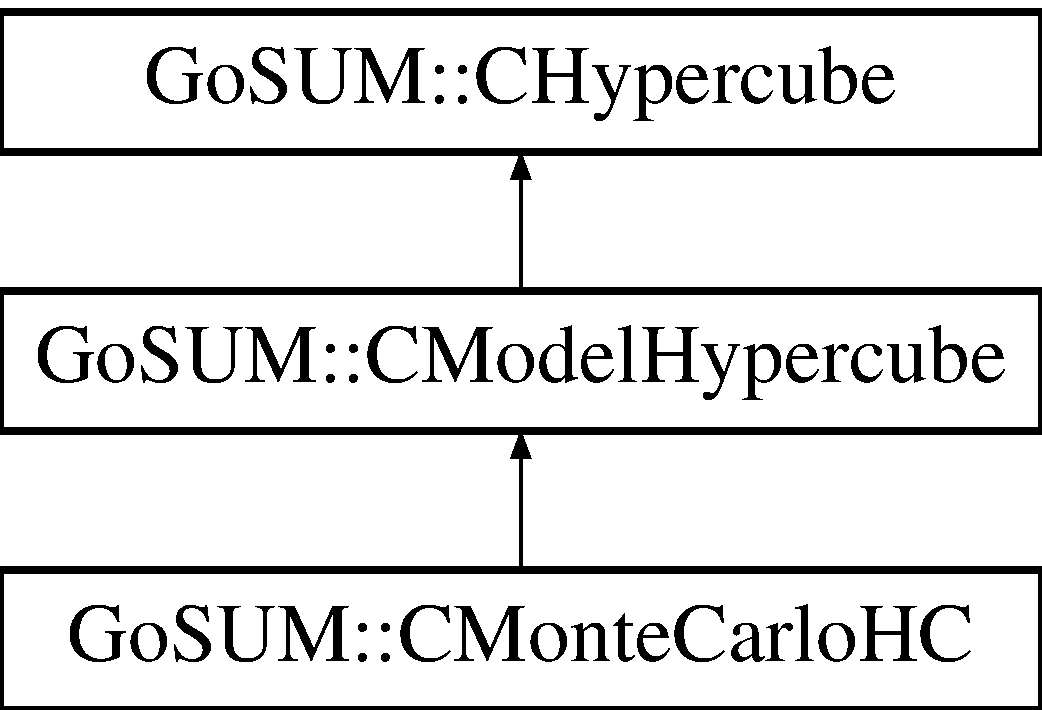
\includegraphics[height=3.000000cm]{class_go_s_u_m_1_1_c_monte_carlo_h_c}
\end{center}
\end{figure}
\subsection*{Public Member Functions}
\begin{DoxyCompactItemize}
\item 
\hyperlink{class_go_s_u_m_1_1_c_monte_carlo_h_c_a1c2bd67f24a78e2ff904a23f84d83a68}{C\-Monte\-Carlo\-H\-C} (\hyperlink{class_go_s_u_m_1_1_c_input_parameters}{C\-Input\-Parameters} $\ast$\-\_\-p\-I\-P)
\item 
virtual \hyperlink{class_go_s_u_m_1_1_c_monte_carlo_h_c_a0659b61e6b18bfcdb61dac921ac7a2ad}{$\sim$\-C\-Monte\-Carlo\-H\-C} ()
\end{DoxyCompactItemize}
\subsection*{Protected Member Functions}
\begin{DoxyCompactItemize}
\item 
{\footnotesize template$<$class Archive $>$ }\\void \hyperlink{class_go_s_u_m_1_1_c_monte_carlo_h_c_ae04ab348b02072028893eee2541cadf8}{serialize} (Archive \&ar, const unsigned int version)
\item 
virtual void \hyperlink{class_go_s_u_m_1_1_c_monte_carlo_h_c_a848c0dded522350b9d6edb41497e19d1}{do\-Generate} (int \-\_\-rssize, int \-\_\-dim, std\-::vector$<$ Array\-Xd $>$ \&\-\_\-samples)
\begin{DoxyCompactList}\small\item\em Core of the generation. \end{DoxyCompactList}\item 
\hyperlink{class_go_s_u_m_1_1_c_monte_carlo_h_c_a04808b65118e1f197d1af47474bd8f57}{C\-Monte\-Carlo\-H\-C} ()
\end{DoxyCompactItemize}
\subsection*{Friends}
\begin{DoxyCompactItemize}
\item 
class \hyperlink{class_go_s_u_m_1_1_c_monte_carlo_h_c_ac98d07dd8f7b70e16ccb9a01abf56b9c}{boost\-::serialization\-::access}
\begin{DoxyCompactList}\small\item\em Boost serialization. \end{DoxyCompactList}\end{DoxyCompactItemize}
\subsection*{Additional Inherited Members}


\subsection{Constructor \& Destructor Documentation}
\hypertarget{class_go_s_u_m_1_1_c_monte_carlo_h_c_a04808b65118e1f197d1af47474bd8f57}{\index{Go\-S\-U\-M\-::\-C\-Monte\-Carlo\-H\-C@{Go\-S\-U\-M\-::\-C\-Monte\-Carlo\-H\-C}!C\-Monte\-Carlo\-H\-C@{C\-Monte\-Carlo\-H\-C}}
\index{C\-Monte\-Carlo\-H\-C@{C\-Monte\-Carlo\-H\-C}!GoSUM::CMonteCarloHC@{Go\-S\-U\-M\-::\-C\-Monte\-Carlo\-H\-C}}
\subsubsection[{C\-Monte\-Carlo\-H\-C}]{\setlength{\rightskip}{0pt plus 5cm}Go\-S\-U\-M\-::\-C\-Monte\-Carlo\-H\-C\-::\-C\-Monte\-Carlo\-H\-C (
\begin{DoxyParamCaption}
{}
\end{DoxyParamCaption}
)\hspace{0.3cm}{\ttfamily [inline]}, {\ttfamily [protected]}}}\label{class_go_s_u_m_1_1_c_monte_carlo_h_c_a04808b65118e1f197d1af47474bd8f57}
\hypertarget{class_go_s_u_m_1_1_c_monte_carlo_h_c_a1c2bd67f24a78e2ff904a23f84d83a68}{\index{Go\-S\-U\-M\-::\-C\-Monte\-Carlo\-H\-C@{Go\-S\-U\-M\-::\-C\-Monte\-Carlo\-H\-C}!C\-Monte\-Carlo\-H\-C@{C\-Monte\-Carlo\-H\-C}}
\index{C\-Monte\-Carlo\-H\-C@{C\-Monte\-Carlo\-H\-C}!GoSUM::CMonteCarloHC@{Go\-S\-U\-M\-::\-C\-Monte\-Carlo\-H\-C}}
\subsubsection[{C\-Monte\-Carlo\-H\-C}]{\setlength{\rightskip}{0pt plus 5cm}Go\-S\-U\-M\-::\-C\-Monte\-Carlo\-H\-C\-::\-C\-Monte\-Carlo\-H\-C (
\begin{DoxyParamCaption}
\item[{{\bf C\-Input\-Parameters} $\ast$}]{\-\_\-p\-I\-P}
\end{DoxyParamCaption}
)\hspace{0.3cm}{\ttfamily [inline]}}}\label{class_go_s_u_m_1_1_c_monte_carlo_h_c_a1c2bd67f24a78e2ff904a23f84d83a68}
\hypertarget{class_go_s_u_m_1_1_c_monte_carlo_h_c_a0659b61e6b18bfcdb61dac921ac7a2ad}{\index{Go\-S\-U\-M\-::\-C\-Monte\-Carlo\-H\-C@{Go\-S\-U\-M\-::\-C\-Monte\-Carlo\-H\-C}!$\sim$\-C\-Monte\-Carlo\-H\-C@{$\sim$\-C\-Monte\-Carlo\-H\-C}}
\index{$\sim$\-C\-Monte\-Carlo\-H\-C@{$\sim$\-C\-Monte\-Carlo\-H\-C}!GoSUM::CMonteCarloHC@{Go\-S\-U\-M\-::\-C\-Monte\-Carlo\-H\-C}}
\subsubsection[{$\sim$\-C\-Monte\-Carlo\-H\-C}]{\setlength{\rightskip}{0pt plus 5cm}virtual Go\-S\-U\-M\-::\-C\-Monte\-Carlo\-H\-C\-::$\sim$\-C\-Monte\-Carlo\-H\-C (
\begin{DoxyParamCaption}
{}
\end{DoxyParamCaption}
)\hspace{0.3cm}{\ttfamily [inline]}, {\ttfamily [virtual]}}}\label{class_go_s_u_m_1_1_c_monte_carlo_h_c_a0659b61e6b18bfcdb61dac921ac7a2ad}


\subsection{Member Function Documentation}
\hypertarget{class_go_s_u_m_1_1_c_monte_carlo_h_c_a848c0dded522350b9d6edb41497e19d1}{\index{Go\-S\-U\-M\-::\-C\-Monte\-Carlo\-H\-C@{Go\-S\-U\-M\-::\-C\-Monte\-Carlo\-H\-C}!do\-Generate@{do\-Generate}}
\index{do\-Generate@{do\-Generate}!GoSUM::CMonteCarloHC@{Go\-S\-U\-M\-::\-C\-Monte\-Carlo\-H\-C}}
\subsubsection[{do\-Generate}]{\setlength{\rightskip}{0pt plus 5cm}void Go\-S\-U\-M\-::\-C\-Monte\-Carlo\-H\-C\-::do\-Generate (
\begin{DoxyParamCaption}
\item[{int}]{\-\_\-rssize, }
\item[{int}]{\-\_\-dim, }
\item[{std\-::vector$<$ Array\-Xd $>$ \&}]{\-\_\-samples}
\end{DoxyParamCaption}
)\hspace{0.3cm}{\ttfamily [protected]}, {\ttfamily [virtual]}}}\label{class_go_s_u_m_1_1_c_monte_carlo_h_c_a848c0dded522350b9d6edb41497e19d1}


Core of the generation. 



Implements \hyperlink{class_go_s_u_m_1_1_c_model_hypercube_a1e92dd784f1c20b604fecd1a48bea2f4}{Go\-S\-U\-M\-::\-C\-Model\-Hypercube}.

\hypertarget{class_go_s_u_m_1_1_c_monte_carlo_h_c_ae04ab348b02072028893eee2541cadf8}{\index{Go\-S\-U\-M\-::\-C\-Monte\-Carlo\-H\-C@{Go\-S\-U\-M\-::\-C\-Monte\-Carlo\-H\-C}!serialize@{serialize}}
\index{serialize@{serialize}!GoSUM::CMonteCarloHC@{Go\-S\-U\-M\-::\-C\-Monte\-Carlo\-H\-C}}
\subsubsection[{serialize}]{\setlength{\rightskip}{0pt plus 5cm}template$<$class Archive $>$ void Go\-S\-U\-M\-::\-C\-Monte\-Carlo\-H\-C\-::serialize (
\begin{DoxyParamCaption}
\item[{Archive \&}]{ar, }
\item[{const unsigned int}]{version}
\end{DoxyParamCaption}
)\hspace{0.3cm}{\ttfamily [protected]}}}\label{class_go_s_u_m_1_1_c_monte_carlo_h_c_ae04ab348b02072028893eee2541cadf8}


Reimplemented from \hyperlink{class_go_s_u_m_1_1_c_model_hypercube_a67de6632c6f6ca3685d2a750599974c6}{Go\-S\-U\-M\-::\-C\-Model\-Hypercube}.



\subsection{Friends And Related Function Documentation}
\hypertarget{class_go_s_u_m_1_1_c_monte_carlo_h_c_ac98d07dd8f7b70e16ccb9a01abf56b9c}{\index{Go\-S\-U\-M\-::\-C\-Monte\-Carlo\-H\-C@{Go\-S\-U\-M\-::\-C\-Monte\-Carlo\-H\-C}!boost\-::serialization\-::access@{boost\-::serialization\-::access}}
\index{boost\-::serialization\-::access@{boost\-::serialization\-::access}!GoSUM::CMonteCarloHC@{Go\-S\-U\-M\-::\-C\-Monte\-Carlo\-H\-C}}
\subsubsection[{boost\-::serialization\-::access}]{\setlength{\rightskip}{0pt plus 5cm}friend class boost\-::serialization\-::access\hspace{0.3cm}{\ttfamily [friend]}}}\label{class_go_s_u_m_1_1_c_monte_carlo_h_c_ac98d07dd8f7b70e16ccb9a01abf56b9c}


Boost serialization. 



The documentation for this class was generated from the following files\-:\begin{DoxyCompactItemize}
\item 
C\-:/\-Development/core/\hyperlink{_hypercube_8h}{Hypercube.\-h}\item 
C\-:/\-Development/core/\hyperlink{_hypercube_8cpp}{Hypercube.\-cpp}\end{DoxyCompactItemize}

\hypertarget{class_c_n_l_c_r_n_g}{\section{C\-N\-L\-C\-R\-N\-G Class Reference}
\label{class_c_n_l_c_r_n_g}\index{C\-N\-L\-C\-R\-N\-G@{C\-N\-L\-C\-R\-N\-G}}
}


{\ttfamily \#include $<$Random\-Generators.\-h$>$}

Inheritance diagram for C\-N\-L\-C\-R\-N\-G\-:\begin{figure}[H]
\begin{center}
\leavevmode
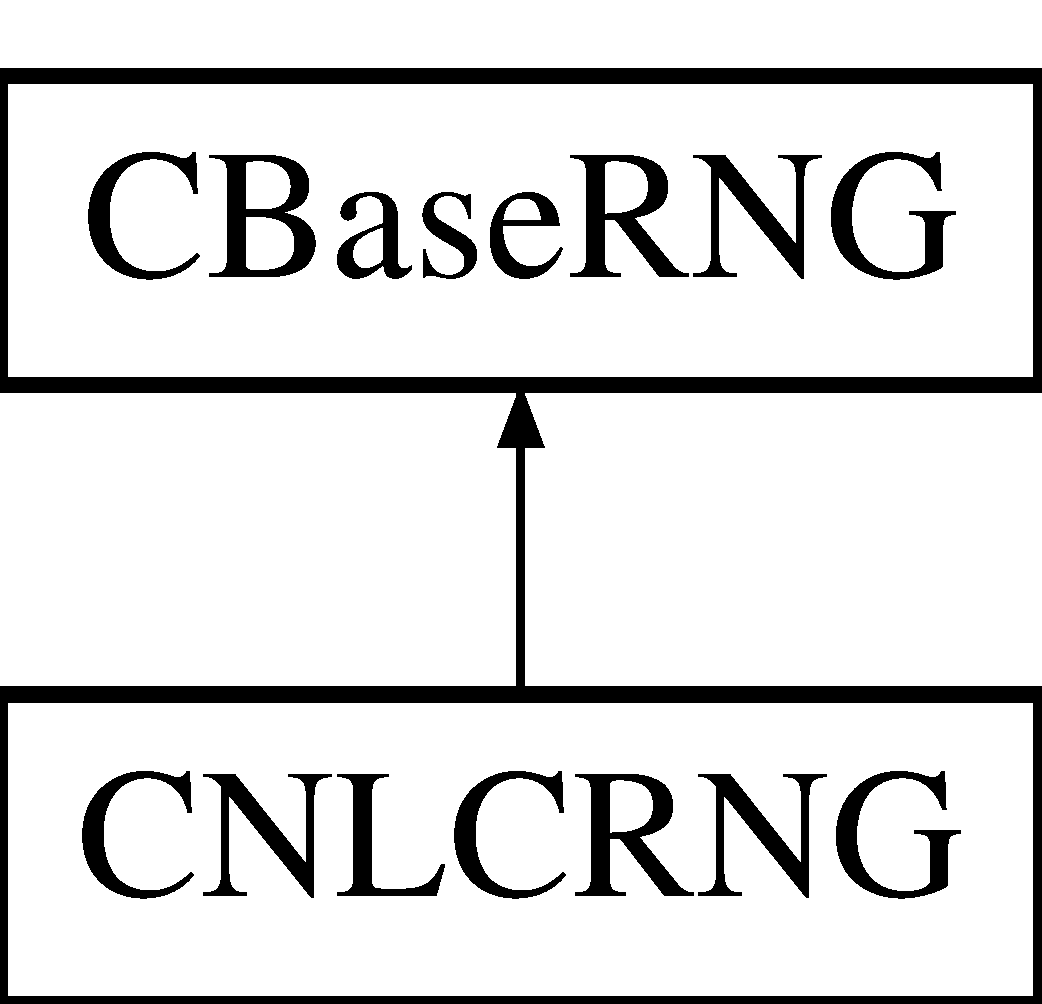
\includegraphics[height=2.000000cm]{class_c_n_l_c_r_n_g}
\end{center}
\end{figure}
\subsection*{Public Member Functions}
\begin{DoxyCompactItemize}
\item 
\hyperlink{class_c_n_l_c_r_n_g_a5d7202006a1e561b71687aa8088fe03f}{C\-N\-L\-C\-R\-N\-G} ()
\item 
\hyperlink{class_c_n_l_c_r_n_g_a9fbafb2eaa13d24b080890e50300dad3}{C\-N\-L\-C\-R\-N\-G} (unsigned int s)
\item 
virtual \hyperlink{class_c_n_l_c_r_n_g_a2631905fcd81aaa129a568dc569100a4}{$\sim$\-C\-N\-L\-C\-R\-N\-G} ()
\item 
virtual void \hyperlink{class_c_n_l_c_r_n_g_a9f6321c4d53774b0c017c6e18124d495}{set\-Seed} (unsigned int s)
\begin{DoxyCompactList}\small\item\em Sets seed of the R\-N\-G. \end{DoxyCompactList}\item 
virtual unsigned int \hyperlink{class_c_n_l_c_r_n_g_a531b9ca98fc7934c90759c1733618298}{rndi} ()
\begin{DoxyCompactList}\small\item\em Returns randomly generated unsigned int. \end{DoxyCompactList}\item 
virtual double \hyperlink{class_c_n_l_c_r_n_g_a5f4f420ffb9147d9edb25b4d49ac05a5}{rnd} ()
\begin{DoxyCompactList}\small\item\em Returns randomly generated double between 0 and 1. \end{DoxyCompactList}\end{DoxyCompactItemize}
\subsection*{Static Private Attributes}
\begin{DoxyCompactItemize}
\item 
static int \hyperlink{class_c_n_l_c_r_n_g_a47b1286233faf1258a8f80efceb9755f}{inext}
\item 
static int \hyperlink{class_c_n_l_c_r_n_g_a1494412ce498bba1816cded65eb5c7a8}{inextp}
\begin{DoxyCompactList}\small\item\em Paramters of the nlc R\-N\-G. \end{DoxyCompactList}\item 
static long \hyperlink{class_c_n_l_c_r_n_g_a8914193c82393d27b6343f47dd750267}{ma} \mbox{[}56\mbox{]}
\begin{DoxyCompactList}\small\item\em Paramters of the nlc R\-N\-G. \end{DoxyCompactList}\end{DoxyCompactItemize}


\subsection{Constructor \& Destructor Documentation}
\hypertarget{class_c_n_l_c_r_n_g_a5d7202006a1e561b71687aa8088fe03f}{\index{C\-N\-L\-C\-R\-N\-G@{C\-N\-L\-C\-R\-N\-G}!C\-N\-L\-C\-R\-N\-G@{C\-N\-L\-C\-R\-N\-G}}
\index{C\-N\-L\-C\-R\-N\-G@{C\-N\-L\-C\-R\-N\-G}!CNLCRNG@{C\-N\-L\-C\-R\-N\-G}}
\subsubsection[{C\-N\-L\-C\-R\-N\-G}]{\setlength{\rightskip}{0pt plus 5cm}C\-N\-L\-C\-R\-N\-G\-::\-C\-N\-L\-C\-R\-N\-G (
\begin{DoxyParamCaption}
{}
\end{DoxyParamCaption}
)\hspace{0.3cm}{\ttfamily [inline]}}}\label{class_c_n_l_c_r_n_g_a5d7202006a1e561b71687aa8088fe03f}
\hypertarget{class_c_n_l_c_r_n_g_a9fbafb2eaa13d24b080890e50300dad3}{\index{C\-N\-L\-C\-R\-N\-G@{C\-N\-L\-C\-R\-N\-G}!C\-N\-L\-C\-R\-N\-G@{C\-N\-L\-C\-R\-N\-G}}
\index{C\-N\-L\-C\-R\-N\-G@{C\-N\-L\-C\-R\-N\-G}!CNLCRNG@{C\-N\-L\-C\-R\-N\-G}}
\subsubsection[{C\-N\-L\-C\-R\-N\-G}]{\setlength{\rightskip}{0pt plus 5cm}C\-N\-L\-C\-R\-N\-G\-::\-C\-N\-L\-C\-R\-N\-G (
\begin{DoxyParamCaption}
\item[{unsigned int}]{s}
\end{DoxyParamCaption}
)\hspace{0.3cm}{\ttfamily [inline]}}}\label{class_c_n_l_c_r_n_g_a9fbafb2eaa13d24b080890e50300dad3}
\hypertarget{class_c_n_l_c_r_n_g_a2631905fcd81aaa129a568dc569100a4}{\index{C\-N\-L\-C\-R\-N\-G@{C\-N\-L\-C\-R\-N\-G}!$\sim$\-C\-N\-L\-C\-R\-N\-G@{$\sim$\-C\-N\-L\-C\-R\-N\-G}}
\index{$\sim$\-C\-N\-L\-C\-R\-N\-G@{$\sim$\-C\-N\-L\-C\-R\-N\-G}!CNLCRNG@{C\-N\-L\-C\-R\-N\-G}}
\subsubsection[{$\sim$\-C\-N\-L\-C\-R\-N\-G}]{\setlength{\rightskip}{0pt plus 5cm}virtual C\-N\-L\-C\-R\-N\-G\-::$\sim$\-C\-N\-L\-C\-R\-N\-G (
\begin{DoxyParamCaption}
{}
\end{DoxyParamCaption}
)\hspace{0.3cm}{\ttfamily [inline]}, {\ttfamily [virtual]}}}\label{class_c_n_l_c_r_n_g_a2631905fcd81aaa129a568dc569100a4}


\subsection{Member Function Documentation}
\hypertarget{class_c_n_l_c_r_n_g_a5f4f420ffb9147d9edb25b4d49ac05a5}{\index{C\-N\-L\-C\-R\-N\-G@{C\-N\-L\-C\-R\-N\-G}!rnd@{rnd}}
\index{rnd@{rnd}!CNLCRNG@{C\-N\-L\-C\-R\-N\-G}}
\subsubsection[{rnd}]{\setlength{\rightskip}{0pt plus 5cm}double C\-N\-L\-C\-R\-N\-G\-::rnd (
\begin{DoxyParamCaption}
{}
\end{DoxyParamCaption}
)\hspace{0.3cm}{\ttfamily [virtual]}}}\label{class_c_n_l_c_r_n_g_a5f4f420ffb9147d9edb25b4d49ac05a5}


Returns randomly generated double between 0 and 1. 



Implements \hyperlink{class_c_base_r_n_g_abbd60a5ecdc9502dd646434224ab5d6b}{C\-Base\-R\-N\-G}.

\hypertarget{class_c_n_l_c_r_n_g_a531b9ca98fc7934c90759c1733618298}{\index{C\-N\-L\-C\-R\-N\-G@{C\-N\-L\-C\-R\-N\-G}!rndi@{rndi}}
\index{rndi@{rndi}!CNLCRNG@{C\-N\-L\-C\-R\-N\-G}}
\subsubsection[{rndi}]{\setlength{\rightskip}{0pt plus 5cm}virtual unsigned int C\-N\-L\-C\-R\-N\-G\-::rndi (
\begin{DoxyParamCaption}
{}
\end{DoxyParamCaption}
)\hspace{0.3cm}{\ttfamily [inline]}, {\ttfamily [virtual]}}}\label{class_c_n_l_c_r_n_g_a531b9ca98fc7934c90759c1733618298}


Returns randomly generated unsigned int. 



Implements \hyperlink{class_c_base_r_n_g_a2db96fbf06a2f11b3613d422043fb7b8}{C\-Base\-R\-N\-G}.

\hypertarget{class_c_n_l_c_r_n_g_a9f6321c4d53774b0c017c6e18124d495}{\index{C\-N\-L\-C\-R\-N\-G@{C\-N\-L\-C\-R\-N\-G}!set\-Seed@{set\-Seed}}
\index{set\-Seed@{set\-Seed}!CNLCRNG@{C\-N\-L\-C\-R\-N\-G}}
\subsubsection[{set\-Seed}]{\setlength{\rightskip}{0pt plus 5cm}void C\-N\-L\-C\-R\-N\-G\-::set\-Seed (
\begin{DoxyParamCaption}
\item[{unsigned int}]{s}
\end{DoxyParamCaption}
)\hspace{0.3cm}{\ttfamily [virtual]}}}\label{class_c_n_l_c_r_n_g_a9f6321c4d53774b0c017c6e18124d495}


Sets seed of the R\-N\-G. 



Implements \hyperlink{class_c_base_r_n_g_a56fbf75ca07b73954596ee04820e0b07}{C\-Base\-R\-N\-G}.



\subsection{Member Data Documentation}
\hypertarget{class_c_n_l_c_r_n_g_a47b1286233faf1258a8f80efceb9755f}{\index{C\-N\-L\-C\-R\-N\-G@{C\-N\-L\-C\-R\-N\-G}!inext@{inext}}
\index{inext@{inext}!CNLCRNG@{C\-N\-L\-C\-R\-N\-G}}
\subsubsection[{inext}]{\setlength{\rightskip}{0pt plus 5cm}int C\-N\-L\-C\-R\-N\-G\-::inext\hspace{0.3cm}{\ttfamily [static]}, {\ttfamily [private]}}}\label{class_c_n_l_c_r_n_g_a47b1286233faf1258a8f80efceb9755f}
\hypertarget{class_c_n_l_c_r_n_g_a1494412ce498bba1816cded65eb5c7a8}{\index{C\-N\-L\-C\-R\-N\-G@{C\-N\-L\-C\-R\-N\-G}!inextp@{inextp}}
\index{inextp@{inextp}!CNLCRNG@{C\-N\-L\-C\-R\-N\-G}}
\subsubsection[{inextp}]{\setlength{\rightskip}{0pt plus 5cm}int C\-N\-L\-C\-R\-N\-G\-::inextp\hspace{0.3cm}{\ttfamily [static]}, {\ttfamily [private]}}}\label{class_c_n_l_c_r_n_g_a1494412ce498bba1816cded65eb5c7a8}


Paramters of the nlc R\-N\-G. 

\hypertarget{class_c_n_l_c_r_n_g_a8914193c82393d27b6343f47dd750267}{\index{C\-N\-L\-C\-R\-N\-G@{C\-N\-L\-C\-R\-N\-G}!ma@{ma}}
\index{ma@{ma}!CNLCRNG@{C\-N\-L\-C\-R\-N\-G}}
\subsubsection[{ma}]{\setlength{\rightskip}{0pt plus 5cm}long C\-N\-L\-C\-R\-N\-G\-::ma\hspace{0.3cm}{\ttfamily [static]}, {\ttfamily [private]}}}\label{class_c_n_l_c_r_n_g_a8914193c82393d27b6343f47dd750267}


Paramters of the nlc R\-N\-G. 



The documentation for this class was generated from the following files\-:\begin{DoxyCompactItemize}
\item 
C\-:/\-Development/core/\hyperlink{_random_generators_8h}{Random\-Generators.\-h}\item 
C\-:/\-Development/core/\hyperlink{_random_generators_8cpp}{Random\-Generators.\-cpp}\end{DoxyCompactItemize}

\hypertarget{class_c_nomad_r_n_g}{\section{C\-Nomad\-R\-N\-G Class Reference}
\label{class_c_nomad_r_n_g}\index{C\-Nomad\-R\-N\-G@{C\-Nomad\-R\-N\-G}}
}


Class for N\-O\-M\-A\-D R\-N\-G with period = 2$^\wedge$96-\/1.  




{\ttfamily \#include $<$Random\-Generators.\-h$>$}

Inheritance diagram for C\-Nomad\-R\-N\-G\-:\begin{figure}[H]
\begin{center}
\leavevmode
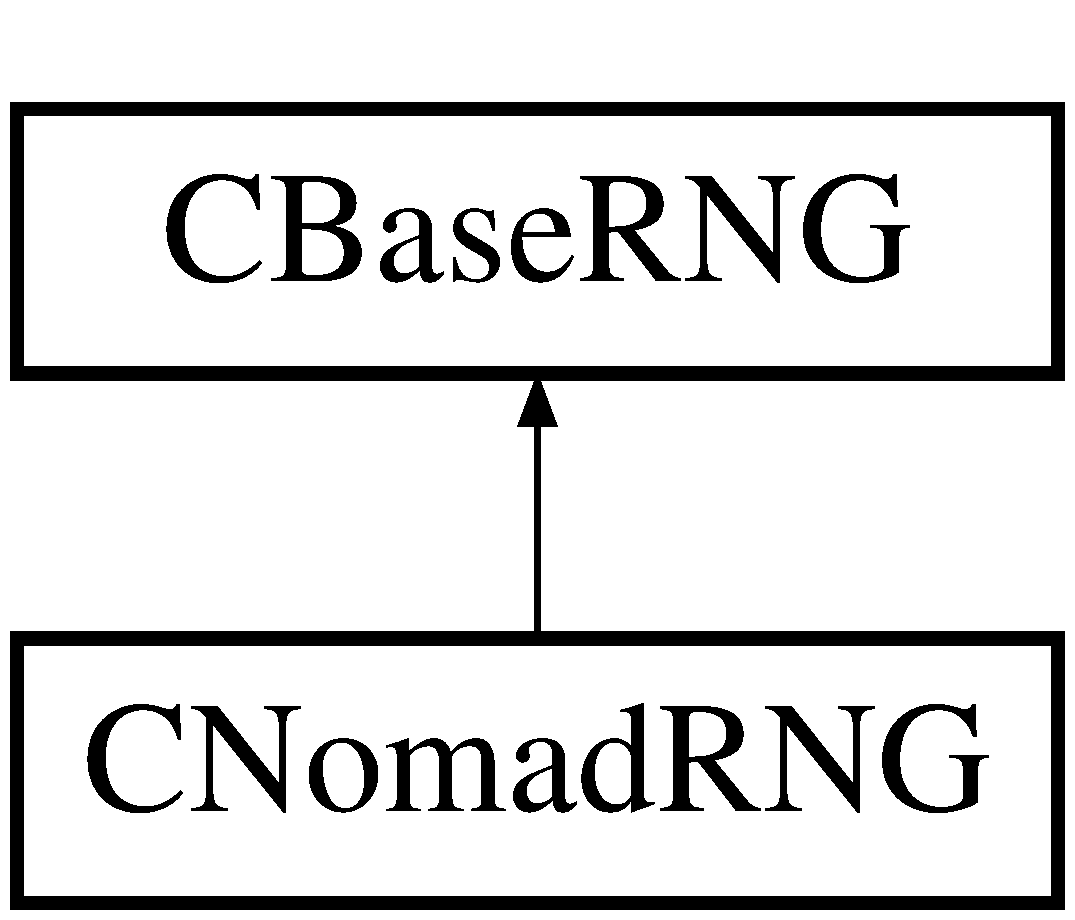
\includegraphics[height=2.000000cm]{class_c_nomad_r_n_g}
\end{center}
\end{figure}
\subsection*{Public Member Functions}
\begin{DoxyCompactItemize}
\item 
\hyperlink{class_c_nomad_r_n_g_a1451ce12dd43333a0c0af7668ae3695a}{C\-Nomad\-R\-N\-G} ()
\item 
\hyperlink{class_c_nomad_r_n_g_ae0c0e56faad80fec2a71ce4fb3686a78}{C\-Nomad\-R\-N\-G} (unsigned int s)
\item 
virtual \hyperlink{class_c_nomad_r_n_g_ad8052941c7b1dc31aba60356aa506daf}{$\sim$\-C\-Nomad\-R\-N\-G} ()
\item 
virtual void \hyperlink{class_c_nomad_r_n_g_a6cedb9431179cee4677d415c8e7611c3}{set\-Seed} (unsigned int s)
\begin{DoxyCompactList}\small\item\em Sets seed of the R\-N\-G. \end{DoxyCompactList}\item 
virtual unsigned int \hyperlink{class_c_nomad_r_n_g_ad41c27377065df6efdadc2d1b30ca315}{rndi} ()
\begin{DoxyCompactList}\small\item\em Returns randomly generated unsigned int. \end{DoxyCompactList}\item 
virtual double \hyperlink{class_c_nomad_r_n_g_a80ec634087f50ef6753f1c5fe24c7ad4}{rnd} ()
\begin{DoxyCompactList}\small\item\em Returns randomly generated double between 0 and 1. \end{DoxyCompactList}\end{DoxyCompactItemize}
\subsection*{Static Private Attributes}
\begin{DoxyCompactItemize}
\item 
static unsigned int \hyperlink{class_c_nomad_r_n_g_ac5867625fe6608450421de3166e38fd8}{x} = 123456789
\item 
static unsigned int \hyperlink{class_c_nomad_r_n_g_ae5ab3fef08b3818ae0b72d7f705cbb07}{y} = 362436069
\item 
static unsigned int \hyperlink{class_c_nomad_r_n_g_ad566dc723566cf9c6ec324b3ef1cc008}{z} = 521288629
\end{DoxyCompactItemize}


\subsection{Detailed Description}
Class for N\-O\-M\-A\-D R\-N\-G with period = 2$^\wedge$96-\/1. 

\subsection{Constructor \& Destructor Documentation}
\hypertarget{class_c_nomad_r_n_g_a1451ce12dd43333a0c0af7668ae3695a}{\index{C\-Nomad\-R\-N\-G@{C\-Nomad\-R\-N\-G}!C\-Nomad\-R\-N\-G@{C\-Nomad\-R\-N\-G}}
\index{C\-Nomad\-R\-N\-G@{C\-Nomad\-R\-N\-G}!CNomadRNG@{C\-Nomad\-R\-N\-G}}
\subsubsection[{C\-Nomad\-R\-N\-G}]{\setlength{\rightskip}{0pt plus 5cm}C\-Nomad\-R\-N\-G\-::\-C\-Nomad\-R\-N\-G (
\begin{DoxyParamCaption}
{}
\end{DoxyParamCaption}
)\hspace{0.3cm}{\ttfamily [inline]}}}\label{class_c_nomad_r_n_g_a1451ce12dd43333a0c0af7668ae3695a}
\hypertarget{class_c_nomad_r_n_g_ae0c0e56faad80fec2a71ce4fb3686a78}{\index{C\-Nomad\-R\-N\-G@{C\-Nomad\-R\-N\-G}!C\-Nomad\-R\-N\-G@{C\-Nomad\-R\-N\-G}}
\index{C\-Nomad\-R\-N\-G@{C\-Nomad\-R\-N\-G}!CNomadRNG@{C\-Nomad\-R\-N\-G}}
\subsubsection[{C\-Nomad\-R\-N\-G}]{\setlength{\rightskip}{0pt plus 5cm}C\-Nomad\-R\-N\-G\-::\-C\-Nomad\-R\-N\-G (
\begin{DoxyParamCaption}
\item[{unsigned int}]{s}
\end{DoxyParamCaption}
)\hspace{0.3cm}{\ttfamily [inline]}}}\label{class_c_nomad_r_n_g_ae0c0e56faad80fec2a71ce4fb3686a78}
\hypertarget{class_c_nomad_r_n_g_ad8052941c7b1dc31aba60356aa506daf}{\index{C\-Nomad\-R\-N\-G@{C\-Nomad\-R\-N\-G}!$\sim$\-C\-Nomad\-R\-N\-G@{$\sim$\-C\-Nomad\-R\-N\-G}}
\index{$\sim$\-C\-Nomad\-R\-N\-G@{$\sim$\-C\-Nomad\-R\-N\-G}!CNomadRNG@{C\-Nomad\-R\-N\-G}}
\subsubsection[{$\sim$\-C\-Nomad\-R\-N\-G}]{\setlength{\rightskip}{0pt plus 5cm}virtual C\-Nomad\-R\-N\-G\-::$\sim$\-C\-Nomad\-R\-N\-G (
\begin{DoxyParamCaption}
{}
\end{DoxyParamCaption}
)\hspace{0.3cm}{\ttfamily [inline]}, {\ttfamily [virtual]}}}\label{class_c_nomad_r_n_g_ad8052941c7b1dc31aba60356aa506daf}


\subsection{Member Function Documentation}
\hypertarget{class_c_nomad_r_n_g_a80ec634087f50ef6753f1c5fe24c7ad4}{\index{C\-Nomad\-R\-N\-G@{C\-Nomad\-R\-N\-G}!rnd@{rnd}}
\index{rnd@{rnd}!CNomadRNG@{C\-Nomad\-R\-N\-G}}
\subsubsection[{rnd}]{\setlength{\rightskip}{0pt plus 5cm}virtual double C\-Nomad\-R\-N\-G\-::rnd (
\begin{DoxyParamCaption}
{}
\end{DoxyParamCaption}
)\hspace{0.3cm}{\ttfamily [inline]}, {\ttfamily [virtual]}}}\label{class_c_nomad_r_n_g_a80ec634087f50ef6753f1c5fe24c7ad4}


Returns randomly generated double between 0 and 1. 



Implements \hyperlink{class_c_base_r_n_g_abbd60a5ecdc9502dd646434224ab5d6b}{C\-Base\-R\-N\-G}.

\hypertarget{class_c_nomad_r_n_g_ad41c27377065df6efdadc2d1b30ca315}{\index{C\-Nomad\-R\-N\-G@{C\-Nomad\-R\-N\-G}!rndi@{rndi}}
\index{rndi@{rndi}!CNomadRNG@{C\-Nomad\-R\-N\-G}}
\subsubsection[{rndi}]{\setlength{\rightskip}{0pt plus 5cm}unsigned int C\-Nomad\-R\-N\-G\-::rndi (
\begin{DoxyParamCaption}
{}
\end{DoxyParamCaption}
)\hspace{0.3cm}{\ttfamily [virtual]}}}\label{class_c_nomad_r_n_g_ad41c27377065df6efdadc2d1b30ca315}


Returns randomly generated unsigned int. 



Implements \hyperlink{class_c_base_r_n_g_a2db96fbf06a2f11b3613d422043fb7b8}{C\-Base\-R\-N\-G}.

\hypertarget{class_c_nomad_r_n_g_a6cedb9431179cee4677d415c8e7611c3}{\index{C\-Nomad\-R\-N\-G@{C\-Nomad\-R\-N\-G}!set\-Seed@{set\-Seed}}
\index{set\-Seed@{set\-Seed}!CNomadRNG@{C\-Nomad\-R\-N\-G}}
\subsubsection[{set\-Seed}]{\setlength{\rightskip}{0pt plus 5cm}virtual void C\-Nomad\-R\-N\-G\-::set\-Seed (
\begin{DoxyParamCaption}
\item[{unsigned int}]{s}
\end{DoxyParamCaption}
)\hspace{0.3cm}{\ttfamily [inline]}, {\ttfamily [virtual]}}}\label{class_c_nomad_r_n_g_a6cedb9431179cee4677d415c8e7611c3}


Sets seed of the R\-N\-G. 



Implements \hyperlink{class_c_base_r_n_g_a56fbf75ca07b73954596ee04820e0b07}{C\-Base\-R\-N\-G}.



\subsection{Member Data Documentation}
\hypertarget{class_c_nomad_r_n_g_ac5867625fe6608450421de3166e38fd8}{\index{C\-Nomad\-R\-N\-G@{C\-Nomad\-R\-N\-G}!x@{x}}
\index{x@{x}!CNomadRNG@{C\-Nomad\-R\-N\-G}}
\subsubsection[{x}]{\setlength{\rightskip}{0pt plus 5cm}unsigned int C\-Nomad\-R\-N\-G\-::x = 123456789\hspace{0.3cm}{\ttfamily [static]}, {\ttfamily [private]}}}\label{class_c_nomad_r_n_g_ac5867625fe6608450421de3166e38fd8}
\hypertarget{class_c_nomad_r_n_g_ae5ab3fef08b3818ae0b72d7f705cbb07}{\index{C\-Nomad\-R\-N\-G@{C\-Nomad\-R\-N\-G}!y@{y}}
\index{y@{y}!CNomadRNG@{C\-Nomad\-R\-N\-G}}
\subsubsection[{y}]{\setlength{\rightskip}{0pt plus 5cm}unsigned int C\-Nomad\-R\-N\-G\-::y = 362436069\hspace{0.3cm}{\ttfamily [static]}, {\ttfamily [private]}}}\label{class_c_nomad_r_n_g_ae5ab3fef08b3818ae0b72d7f705cbb07}
\hypertarget{class_c_nomad_r_n_g_ad566dc723566cf9c6ec324b3ef1cc008}{\index{C\-Nomad\-R\-N\-G@{C\-Nomad\-R\-N\-G}!z@{z}}
\index{z@{z}!CNomadRNG@{C\-Nomad\-R\-N\-G}}
\subsubsection[{z}]{\setlength{\rightskip}{0pt plus 5cm}unsigned int C\-Nomad\-R\-N\-G\-::z = 521288629\hspace{0.3cm}{\ttfamily [static]}, {\ttfamily [private]}}}\label{class_c_nomad_r_n_g_ad566dc723566cf9c6ec324b3ef1cc008}


The documentation for this class was generated from the following files\-:\begin{DoxyCompactItemize}
\item 
C\-:/\-Development/core/\hyperlink{_random_generators_8h}{Random\-Generators.\-h}\item 
C\-:/\-Development/core/\hyperlink{_random_generators_8cpp}{Random\-Generators.\-cpp}\end{DoxyCompactItemize}

\hypertarget{class_c_numerical_sample}{\section{C\-Numerical\-Sample Class Reference}
\label{class_c_numerical_sample}\index{C\-Numerical\-Sample@{C\-Numerical\-Sample}}
}


Abstract class for numerical discrete samples.  




{\ttfamily \#include $<$Sample.\-h$>$}

Inheritance diagram for C\-Numerical\-Sample\-:\begin{figure}[H]
\begin{center}
\leavevmode
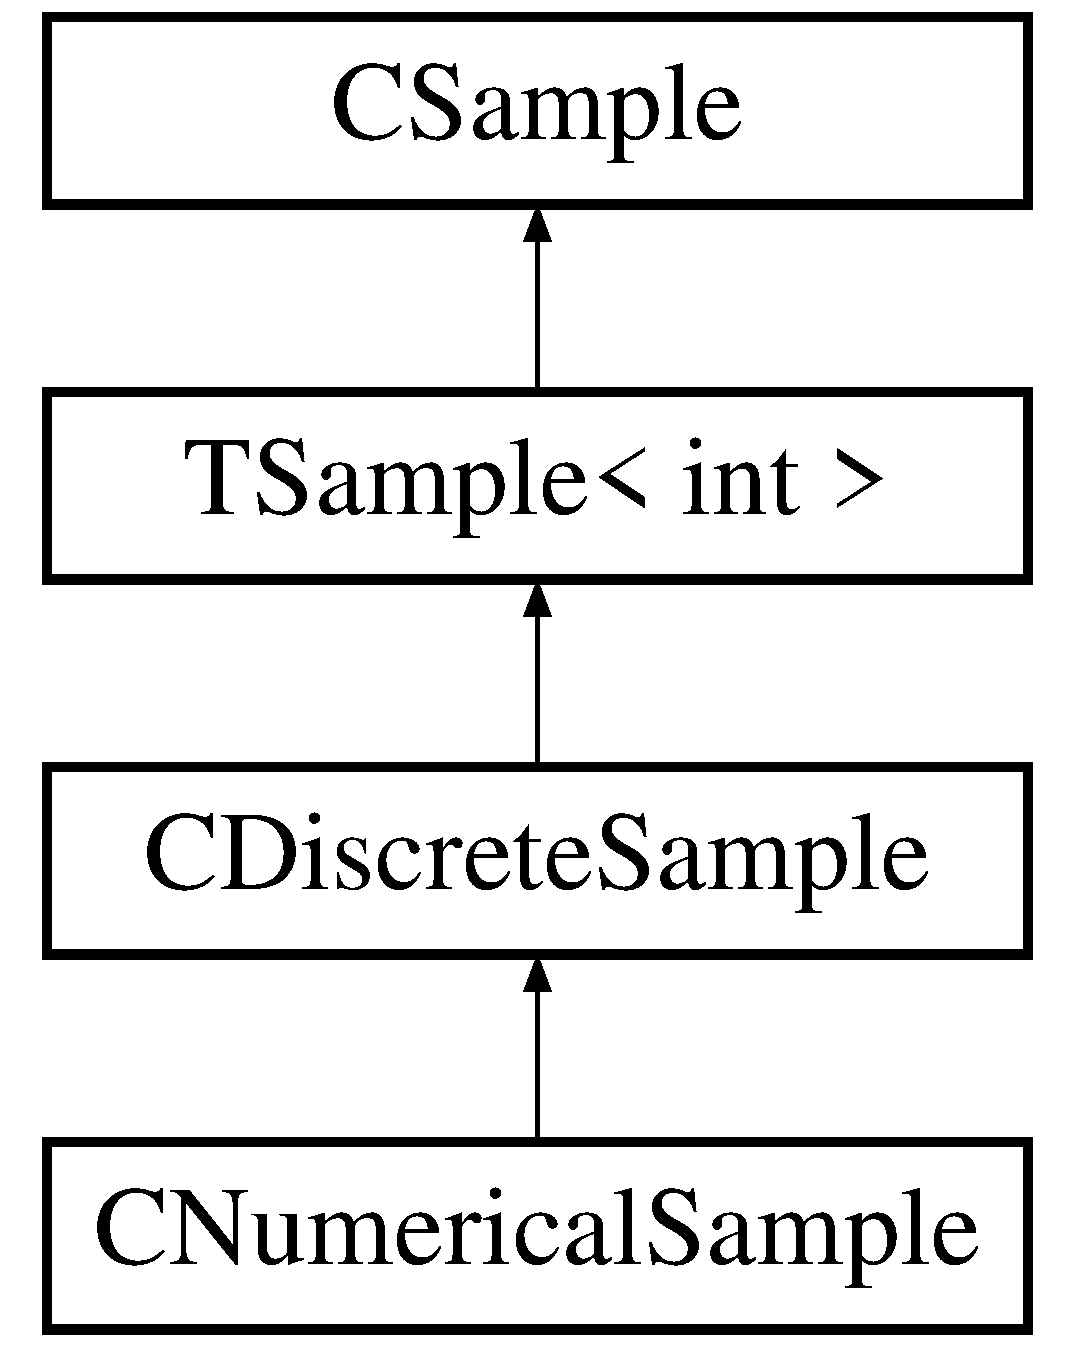
\includegraphics[height=4.000000cm]{class_c_numerical_sample}
\end{center}
\end{figure}
\subsection*{Public Member Functions}
\begin{DoxyCompactItemize}
\item 
\hyperlink{class_c_numerical_sample_a048b81156592132f06e23c4bcf1cd113}{C\-Numerical\-Sample} ()
\item 
\hyperlink{class_c_numerical_sample_ad63a5b9e8440a380a6daa5cdcdc1cd28}{C\-Numerical\-Sample} (const \hyperlink{class_c_numerical_sample}{C\-Numerical\-Sample} \&O)
\item 
\hyperlink{class_c_numerical_sample_accc910ec7b8abfaa9af11346f8bd8cb0}{C\-Numerical\-Sample} (const \hyperlink{class_c_continuous_sample}{C\-Continuous\-Sample} \&O)
\item 
virtual \hyperlink{class_c_numerical_sample_ae1d6f516e0122a2b257a036b1e42da1d}{$\sim$\-C\-Numerical\-Sample} ()
\item 
virtual void \hyperlink{class_c_numerical_sample_a929eddefbbb32c7079e2e60ca95535da}{read\-Sample\-Value} (std\-::ifstream \&\-\_\-ifs, int \-\_\-at)
\begin{DoxyCompactList}\small\item\em Reads particular sample data from input file stream. \end{DoxyCompactList}\item 
virtual void \hyperlink{class_c_numerical_sample_ae1ed83416fc77ab40019c2577047a788}{write\-Sample\-Value} (std\-::ofstream \&\-\_\-ofs, int \-\_\-at) const 
\begin{DoxyCompactList}\small\item\em $<$ Writes particular sample data to output file stream. \end{DoxyCompactList}\item 
virtual void \hyperlink{class_c_numerical_sample_a2a558ba5736bf8893121dd9174110140}{set\-Sample\-Size} (int \-\_\-n)
\begin{DoxyCompactList}\small\item\em Sets particular sample data value. \end{DoxyCompactList}\item 
int \hyperlink{class_c_numerical_sample_a23b6f5afff20a9bd788c49a557702d8c}{min\-Value} () const 
\begin{DoxyCompactList}\small\item\em Returns minimal sample data value. \end{DoxyCompactList}\item 
int \hyperlink{class_c_numerical_sample_ad207c9baed07803c1fb2ac5e285bd896}{max\-Value} () const 
\begin{DoxyCompactList}\small\item\em Returns maximal sample data value. \end{DoxyCompactList}\item 
virtual double \hyperlink{class_c_numerical_sample_aedf72750cb229d9c17417ba787e487f1}{variance} () const 
\begin{DoxyCompactList}\small\item\em Returns sample variance (i.\-e.\-empirical). \end{DoxyCompactList}\end{DoxyCompactItemize}
\subsection*{Private Member Functions}
\begin{DoxyCompactItemize}
\item 
{\footnotesize template$<$class Archive $>$ }\\void \hyperlink{class_c_numerical_sample_a1f1ace88ad7ae05196dcd498b518af3c}{serialize} (Archive \&ar, const unsigned int version)
\end{DoxyCompactItemize}
\subsection*{Private Attributes}
\begin{DoxyCompactItemize}
\item 
std\-::vector$<$ double $>$ \hyperlink{class_c_numerical_sample_a2e2653a81d6c91eafc0548c0e7b50227}{values}
\end{DoxyCompactItemize}
\subsection*{Friends}
\begin{DoxyCompactItemize}
\item 
class \hyperlink{class_c_numerical_sample_ac98d07dd8f7b70e16ccb9a01abf56b9c}{boost\-::serialization\-::access}
\begin{DoxyCompactList}\small\item\em Boost serialization. \end{DoxyCompactList}\end{DoxyCompactItemize}
\subsection*{Additional Inherited Members}


\subsection{Detailed Description}
Abstract class for numerical discrete samples. 

\subsection{Constructor \& Destructor Documentation}
\hypertarget{class_c_numerical_sample_a048b81156592132f06e23c4bcf1cd113}{\index{C\-Numerical\-Sample@{C\-Numerical\-Sample}!C\-Numerical\-Sample@{C\-Numerical\-Sample}}
\index{C\-Numerical\-Sample@{C\-Numerical\-Sample}!CNumericalSample@{C\-Numerical\-Sample}}
\subsubsection[{C\-Numerical\-Sample}]{\setlength{\rightskip}{0pt plus 5cm}C\-Numerical\-Sample\-::\-C\-Numerical\-Sample (
\begin{DoxyParamCaption}
{}
\end{DoxyParamCaption}
)\hspace{0.3cm}{\ttfamily [inline]}}}\label{class_c_numerical_sample_a048b81156592132f06e23c4bcf1cd113}
\hypertarget{class_c_numerical_sample_ad63a5b9e8440a380a6daa5cdcdc1cd28}{\index{C\-Numerical\-Sample@{C\-Numerical\-Sample}!C\-Numerical\-Sample@{C\-Numerical\-Sample}}
\index{C\-Numerical\-Sample@{C\-Numerical\-Sample}!CNumericalSample@{C\-Numerical\-Sample}}
\subsubsection[{C\-Numerical\-Sample}]{\setlength{\rightskip}{0pt plus 5cm}C\-Numerical\-Sample\-::\-C\-Numerical\-Sample (
\begin{DoxyParamCaption}
\item[{const {\bf C\-Numerical\-Sample} \&}]{O}
\end{DoxyParamCaption}
)\hspace{0.3cm}{\ttfamily [inline]}}}\label{class_c_numerical_sample_ad63a5b9e8440a380a6daa5cdcdc1cd28}
\hypertarget{class_c_numerical_sample_accc910ec7b8abfaa9af11346f8bd8cb0}{\index{C\-Numerical\-Sample@{C\-Numerical\-Sample}!C\-Numerical\-Sample@{C\-Numerical\-Sample}}
\index{C\-Numerical\-Sample@{C\-Numerical\-Sample}!CNumericalSample@{C\-Numerical\-Sample}}
\subsubsection[{C\-Numerical\-Sample}]{\setlength{\rightskip}{0pt plus 5cm}C\-Numerical\-Sample\-::\-C\-Numerical\-Sample (
\begin{DoxyParamCaption}
\item[{const {\bf C\-Continuous\-Sample} \&}]{O}
\end{DoxyParamCaption}
)}}\label{class_c_numerical_sample_accc910ec7b8abfaa9af11346f8bd8cb0}
\hypertarget{class_c_numerical_sample_ae1d6f516e0122a2b257a036b1e42da1d}{\index{C\-Numerical\-Sample@{C\-Numerical\-Sample}!$\sim$\-C\-Numerical\-Sample@{$\sim$\-C\-Numerical\-Sample}}
\index{$\sim$\-C\-Numerical\-Sample@{$\sim$\-C\-Numerical\-Sample}!CNumericalSample@{C\-Numerical\-Sample}}
\subsubsection[{$\sim$\-C\-Numerical\-Sample}]{\setlength{\rightskip}{0pt plus 5cm}virtual C\-Numerical\-Sample\-::$\sim$\-C\-Numerical\-Sample (
\begin{DoxyParamCaption}
{}
\end{DoxyParamCaption}
)\hspace{0.3cm}{\ttfamily [inline]}, {\ttfamily [virtual]}}}\label{class_c_numerical_sample_ae1d6f516e0122a2b257a036b1e42da1d}


\subsection{Member Function Documentation}
\hypertarget{class_c_numerical_sample_ad207c9baed07803c1fb2ac5e285bd896}{\index{C\-Numerical\-Sample@{C\-Numerical\-Sample}!max\-Value@{max\-Value}}
\index{max\-Value@{max\-Value}!CNumericalSample@{C\-Numerical\-Sample}}
\subsubsection[{max\-Value}]{\setlength{\rightskip}{0pt plus 5cm}int C\-Numerical\-Sample\-::max\-Value (
\begin{DoxyParamCaption}
{}
\end{DoxyParamCaption}
) const\hspace{0.3cm}{\ttfamily [inline]}}}\label{class_c_numerical_sample_ad207c9baed07803c1fb2ac5e285bd896}


Returns maximal sample data value. 



Reimplemented from \hyperlink{class_t_sample_aac5e27142c09df0a3213a702a5db2a46}{T\-Sample$<$ t $>$}.

\hypertarget{class_c_numerical_sample_a23b6f5afff20a9bd788c49a557702d8c}{\index{C\-Numerical\-Sample@{C\-Numerical\-Sample}!min\-Value@{min\-Value}}
\index{min\-Value@{min\-Value}!CNumericalSample@{C\-Numerical\-Sample}}
\subsubsection[{min\-Value}]{\setlength{\rightskip}{0pt plus 5cm}int C\-Numerical\-Sample\-::min\-Value (
\begin{DoxyParamCaption}
{}
\end{DoxyParamCaption}
) const\hspace{0.3cm}{\ttfamily [inline]}}}\label{class_c_numerical_sample_a23b6f5afff20a9bd788c49a557702d8c}


Returns minimal sample data value. 



Reimplemented from \hyperlink{class_t_sample_a8390ad552199323ae9cc6ab9b17486c6}{T\-Sample$<$ t $>$}.

\hypertarget{class_c_numerical_sample_a929eddefbbb32c7079e2e60ca95535da}{\index{C\-Numerical\-Sample@{C\-Numerical\-Sample}!read\-Sample\-Value@{read\-Sample\-Value}}
\index{read\-Sample\-Value@{read\-Sample\-Value}!CNumericalSample@{C\-Numerical\-Sample}}
\subsubsection[{read\-Sample\-Value}]{\setlength{\rightskip}{0pt plus 5cm}void C\-Numerical\-Sample\-::read\-Sample\-Value (
\begin{DoxyParamCaption}
\item[{std\-::ifstream \&}]{\-\_\-ifs, }
\item[{int}]{\-\_\-at}
\end{DoxyParamCaption}
)\hspace{0.3cm}{\ttfamily [virtual]}}}\label{class_c_numerical_sample_a929eddefbbb32c7079e2e60ca95535da}


Reads particular sample data from input file stream. 



Reimplemented from \hyperlink{class_t_sample_a7a13ccc3ca57276ad789bafd9ceec1d8}{T\-Sample$<$ t $>$}.

\hypertarget{class_c_numerical_sample_a1f1ace88ad7ae05196dcd498b518af3c}{\index{C\-Numerical\-Sample@{C\-Numerical\-Sample}!serialize@{serialize}}
\index{serialize@{serialize}!CNumericalSample@{C\-Numerical\-Sample}}
\subsubsection[{serialize}]{\setlength{\rightskip}{0pt plus 5cm}template$<$class Archive $>$ void C\-Numerical\-Sample\-::serialize (
\begin{DoxyParamCaption}
\item[{Archive \&}]{ar, }
\item[{const unsigned int}]{version}
\end{DoxyParamCaption}
)\hspace{0.3cm}{\ttfamily [private]}}}\label{class_c_numerical_sample_a1f1ace88ad7ae05196dcd498b518af3c}
\hypertarget{class_c_numerical_sample_a2a558ba5736bf8893121dd9174110140}{\index{C\-Numerical\-Sample@{C\-Numerical\-Sample}!set\-Sample\-Size@{set\-Sample\-Size}}
\index{set\-Sample\-Size@{set\-Sample\-Size}!CNumericalSample@{C\-Numerical\-Sample}}
\subsubsection[{set\-Sample\-Size}]{\setlength{\rightskip}{0pt plus 5cm}virtual void C\-Numerical\-Sample\-::set\-Sample\-Size (
\begin{DoxyParamCaption}
\item[{int}]{\-\_\-n}
\end{DoxyParamCaption}
)\hspace{0.3cm}{\ttfamily [inline]}, {\ttfamily [virtual]}}}\label{class_c_numerical_sample_a2a558ba5736bf8893121dd9174110140}


Sets particular sample data value. 



Reimplemented from \hyperlink{class_t_sample_a3b92f468f11169b27a564fd801144fee}{T\-Sample$<$ t $>$}.

\hypertarget{class_c_numerical_sample_aedf72750cb229d9c17417ba787e487f1}{\index{C\-Numerical\-Sample@{C\-Numerical\-Sample}!variance@{variance}}
\index{variance@{variance}!CNumericalSample@{C\-Numerical\-Sample}}
\subsubsection[{variance}]{\setlength{\rightskip}{0pt plus 5cm}virtual double C\-Numerical\-Sample\-::variance (
\begin{DoxyParamCaption}
{}
\end{DoxyParamCaption}
) const\hspace{0.3cm}{\ttfamily [inline]}, {\ttfamily [virtual]}}}\label{class_c_numerical_sample_aedf72750cb229d9c17417ba787e487f1}


Returns sample variance (i.\-e.\-empirical). 



Reimplemented from \hyperlink{class_c_discrete_sample_a3e2d5a72842be01a167f890960a34bef}{C\-Discrete\-Sample}.

\hypertarget{class_c_numerical_sample_ae1ed83416fc77ab40019c2577047a788}{\index{C\-Numerical\-Sample@{C\-Numerical\-Sample}!write\-Sample\-Value@{write\-Sample\-Value}}
\index{write\-Sample\-Value@{write\-Sample\-Value}!CNumericalSample@{C\-Numerical\-Sample}}
\subsubsection[{write\-Sample\-Value}]{\setlength{\rightskip}{0pt plus 5cm}virtual void C\-Numerical\-Sample\-::write\-Sample\-Value (
\begin{DoxyParamCaption}
\item[{std\-::ofstream \&}]{\-\_\-ofs, }
\item[{int}]{\-\_\-at}
\end{DoxyParamCaption}
) const\hspace{0.3cm}{\ttfamily [inline]}, {\ttfamily [virtual]}}}\label{class_c_numerical_sample_ae1ed83416fc77ab40019c2577047a788}


$<$ Writes particular sample data to output file stream. 



Reimplemented from \hyperlink{class_t_sample_abb2feebe92f8fdb290046d6ef0573507}{T\-Sample$<$ t $>$}.



\subsection{Friends And Related Function Documentation}
\hypertarget{class_c_numerical_sample_ac98d07dd8f7b70e16ccb9a01abf56b9c}{\index{C\-Numerical\-Sample@{C\-Numerical\-Sample}!boost\-::serialization\-::access@{boost\-::serialization\-::access}}
\index{boost\-::serialization\-::access@{boost\-::serialization\-::access}!CNumericalSample@{C\-Numerical\-Sample}}
\subsubsection[{boost\-::serialization\-::access}]{\setlength{\rightskip}{0pt plus 5cm}friend class boost\-::serialization\-::access\hspace{0.3cm}{\ttfamily [friend]}}}\label{class_c_numerical_sample_ac98d07dd8f7b70e16ccb9a01abf56b9c}


Boost serialization. 



\subsection{Member Data Documentation}
\hypertarget{class_c_numerical_sample_a2e2653a81d6c91eafc0548c0e7b50227}{\index{C\-Numerical\-Sample@{C\-Numerical\-Sample}!values@{values}}
\index{values@{values}!CNumericalSample@{C\-Numerical\-Sample}}
\subsubsection[{values}]{\setlength{\rightskip}{0pt plus 5cm}std\-::vector$<$double$>$ C\-Numerical\-Sample\-::values\hspace{0.3cm}{\ttfamily [private]}}}\label{class_c_numerical_sample_a2e2653a81d6c91eafc0548c0e7b50227}
Holds all numerical values. 

The documentation for this class was generated from the following files\-:\begin{DoxyCompactItemize}
\item 
C\-:/\-Development/core/\hyperlink{_sample_8h}{Sample.\-h}\item 
C\-:/\-Development/core/\hyperlink{_sample_8cpp}{Sample.\-cpp}\end{DoxyCompactItemize}

\hypertarget{class_go_s_u_m_1_1_c_nu_svc_s_a_m}{\section{Go\-S\-U\-M\-:\-:C\-Nu\-Svc\-S\-A\-M Class Reference}
\label{class_go_s_u_m_1_1_c_nu_svc_s_a_m}\index{Go\-S\-U\-M\-::\-C\-Nu\-Svc\-S\-A\-M@{Go\-S\-U\-M\-::\-C\-Nu\-Svc\-S\-A\-M}}
}


Class for the analyitical model for single output state, nu-\/\-S\-V\-C type.  




{\ttfamily \#include $<$Analytical\-Model.\-h$>$}

Inheritance diagram for Go\-S\-U\-M\-:\-:C\-Nu\-Svc\-S\-A\-M\-:\begin{figure}[H]
\begin{center}
\leavevmode
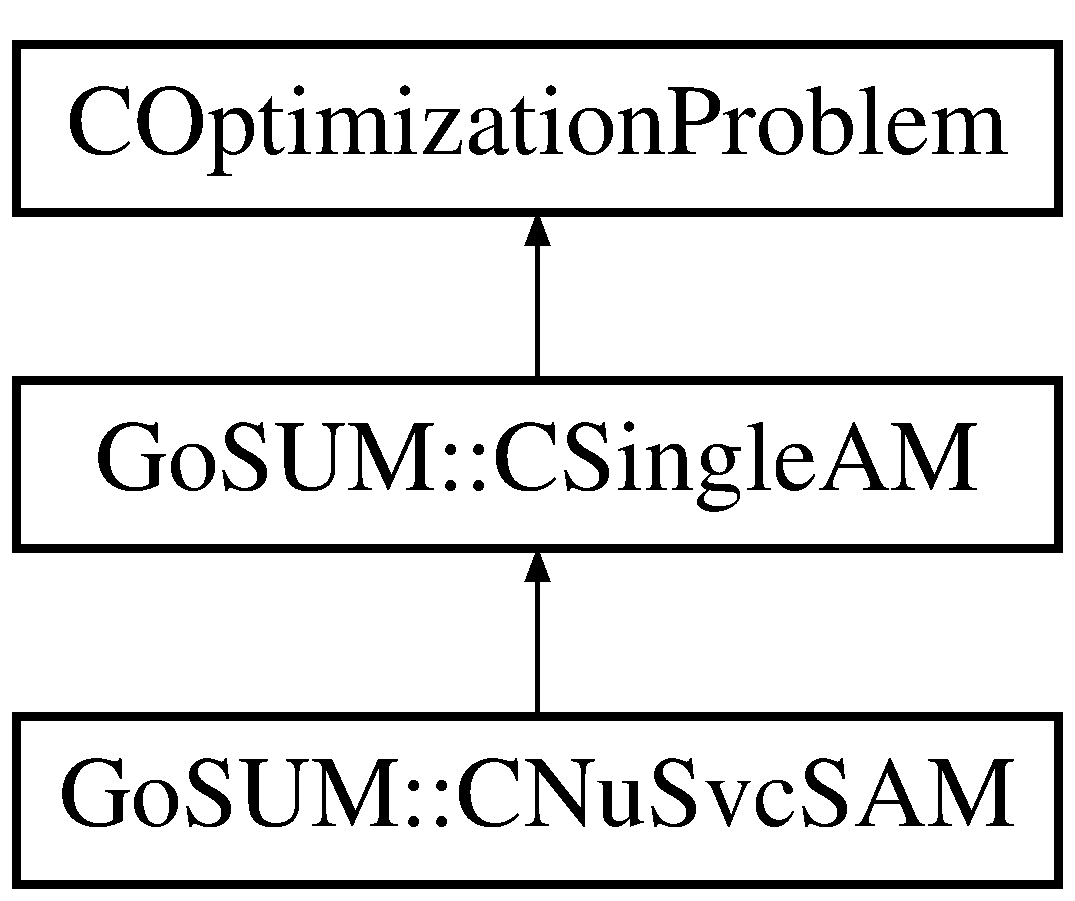
\includegraphics[height=3.000000cm]{class_go_s_u_m_1_1_c_nu_svc_s_a_m}
\end{center}
\end{figure}
\subsection*{Public Member Functions}
\begin{DoxyCompactItemize}
\item 
\hyperlink{class_go_s_u_m_1_1_c_nu_svc_s_a_m_aea0f69fa062d9a74dc15652e532a90b0}{C\-Nu\-Svc\-S\-A\-M} ()
\item 
virtual \hyperlink{class_go_s_u_m_1_1_c_nu_svc_s_a_m_ae07bab5c5cdaf561a6f28cf54153bf54}{$\sim$\-C\-Nu\-Svc\-S\-A\-M} ()
\end{DoxyCompactItemize}
\subsection*{Protected Member Functions}
\begin{DoxyCompactItemize}
\item 
{\footnotesize template$<$class Archive $>$ }\\void \hyperlink{class_go_s_u_m_1_1_c_nu_svc_s_a_m_ac2dab3b5e58ec30ac474f1614bf20873}{serialize} (Archive \&ar, const unsigned int version)
\end{DoxyCompactItemize}
\subsection*{Friends}
\begin{DoxyCompactItemize}
\item 
class \hyperlink{class_go_s_u_m_1_1_c_nu_svc_s_a_m_ac98d07dd8f7b70e16ccb9a01abf56b9c}{boost\-::serialization\-::access}
\begin{DoxyCompactList}\small\item\em Boost serialization. \end{DoxyCompactList}\end{DoxyCompactItemize}
\subsection*{Additional Inherited Members}


\subsection{Detailed Description}
Class for the analyitical model for single output state, nu-\/\-S\-V\-C type. 

\subsection{Constructor \& Destructor Documentation}
\hypertarget{class_go_s_u_m_1_1_c_nu_svc_s_a_m_aea0f69fa062d9a74dc15652e532a90b0}{\index{Go\-S\-U\-M\-::\-C\-Nu\-Svc\-S\-A\-M@{Go\-S\-U\-M\-::\-C\-Nu\-Svc\-S\-A\-M}!C\-Nu\-Svc\-S\-A\-M@{C\-Nu\-Svc\-S\-A\-M}}
\index{C\-Nu\-Svc\-S\-A\-M@{C\-Nu\-Svc\-S\-A\-M}!GoSUM::CNuSvcSAM@{Go\-S\-U\-M\-::\-C\-Nu\-Svc\-S\-A\-M}}
\subsubsection[{C\-Nu\-Svc\-S\-A\-M}]{\setlength{\rightskip}{0pt plus 5cm}Go\-S\-U\-M\-::\-C\-Nu\-Svc\-S\-A\-M\-::\-C\-Nu\-Svc\-S\-A\-M (
\begin{DoxyParamCaption}
{}
\end{DoxyParamCaption}
)\hspace{0.3cm}{\ttfamily [inline]}}}\label{class_go_s_u_m_1_1_c_nu_svc_s_a_m_aea0f69fa062d9a74dc15652e532a90b0}
\hypertarget{class_go_s_u_m_1_1_c_nu_svc_s_a_m_ae07bab5c5cdaf561a6f28cf54153bf54}{\index{Go\-S\-U\-M\-::\-C\-Nu\-Svc\-S\-A\-M@{Go\-S\-U\-M\-::\-C\-Nu\-Svc\-S\-A\-M}!$\sim$\-C\-Nu\-Svc\-S\-A\-M@{$\sim$\-C\-Nu\-Svc\-S\-A\-M}}
\index{$\sim$\-C\-Nu\-Svc\-S\-A\-M@{$\sim$\-C\-Nu\-Svc\-S\-A\-M}!GoSUM::CNuSvcSAM@{Go\-S\-U\-M\-::\-C\-Nu\-Svc\-S\-A\-M}}
\subsubsection[{$\sim$\-C\-Nu\-Svc\-S\-A\-M}]{\setlength{\rightskip}{0pt plus 5cm}virtual Go\-S\-U\-M\-::\-C\-Nu\-Svc\-S\-A\-M\-::$\sim$\-C\-Nu\-Svc\-S\-A\-M (
\begin{DoxyParamCaption}
{}
\end{DoxyParamCaption}
)\hspace{0.3cm}{\ttfamily [inline]}, {\ttfamily [virtual]}}}\label{class_go_s_u_m_1_1_c_nu_svc_s_a_m_ae07bab5c5cdaf561a6f28cf54153bf54}


\subsection{Member Function Documentation}
\hypertarget{class_go_s_u_m_1_1_c_nu_svc_s_a_m_ac2dab3b5e58ec30ac474f1614bf20873}{\index{Go\-S\-U\-M\-::\-C\-Nu\-Svc\-S\-A\-M@{Go\-S\-U\-M\-::\-C\-Nu\-Svc\-S\-A\-M}!serialize@{serialize}}
\index{serialize@{serialize}!GoSUM::CNuSvcSAM@{Go\-S\-U\-M\-::\-C\-Nu\-Svc\-S\-A\-M}}
\subsubsection[{serialize}]{\setlength{\rightskip}{0pt plus 5cm}template$<$class Archive $>$ void Go\-S\-U\-M\-::\-C\-Nu\-Svc\-S\-A\-M\-::serialize (
\begin{DoxyParamCaption}
\item[{Archive \&}]{ar, }
\item[{const unsigned int}]{version}
\end{DoxyParamCaption}
)\hspace{0.3cm}{\ttfamily [protected]}}}\label{class_go_s_u_m_1_1_c_nu_svc_s_a_m_ac2dab3b5e58ec30ac474f1614bf20873}


Reimplemented from \hyperlink{class_go_s_u_m_1_1_c_single_a_m_a761e514fefeb7324e5509571f1be3848}{Go\-S\-U\-M\-::\-C\-Single\-A\-M}.



\subsection{Friends And Related Function Documentation}
\hypertarget{class_go_s_u_m_1_1_c_nu_svc_s_a_m_ac98d07dd8f7b70e16ccb9a01abf56b9c}{\index{Go\-S\-U\-M\-::\-C\-Nu\-Svc\-S\-A\-M@{Go\-S\-U\-M\-::\-C\-Nu\-Svc\-S\-A\-M}!boost\-::serialization\-::access@{boost\-::serialization\-::access}}
\index{boost\-::serialization\-::access@{boost\-::serialization\-::access}!GoSUM::CNuSvcSAM@{Go\-S\-U\-M\-::\-C\-Nu\-Svc\-S\-A\-M}}
\subsubsection[{boost\-::serialization\-::access}]{\setlength{\rightskip}{0pt plus 5cm}friend class boost\-::serialization\-::access\hspace{0.3cm}{\ttfamily [friend]}}}\label{class_go_s_u_m_1_1_c_nu_svc_s_a_m_ac98d07dd8f7b70e16ccb9a01abf56b9c}


Boost serialization. 



The documentation for this class was generated from the following files\-:\begin{DoxyCompactItemize}
\item 
C\-:/\-Development/core/\hyperlink{_analytical_model_8h}{Analytical\-Model.\-h}\item 
C\-:/\-Development/core/\hyperlink{_analytical_model_8cpp}{Analytical\-Model.\-cpp}\end{DoxyCompactItemize}

\hypertarget{class_go_s_u_m_1_1_c_nu_svr_s_a_m}{\section{Go\-S\-U\-M\-:\-:C\-Nu\-Svr\-S\-A\-M Class Reference}
\label{class_go_s_u_m_1_1_c_nu_svr_s_a_m}\index{Go\-S\-U\-M\-::\-C\-Nu\-Svr\-S\-A\-M@{Go\-S\-U\-M\-::\-C\-Nu\-Svr\-S\-A\-M}}
}


Class for the analyitical model for single output state, nu-\/\-S\-V\-R type.  




{\ttfamily \#include $<$Analytical\-Model.\-h$>$}

Inheritance diagram for Go\-S\-U\-M\-:\-:C\-Nu\-Svr\-S\-A\-M\-:\begin{figure}[H]
\begin{center}
\leavevmode
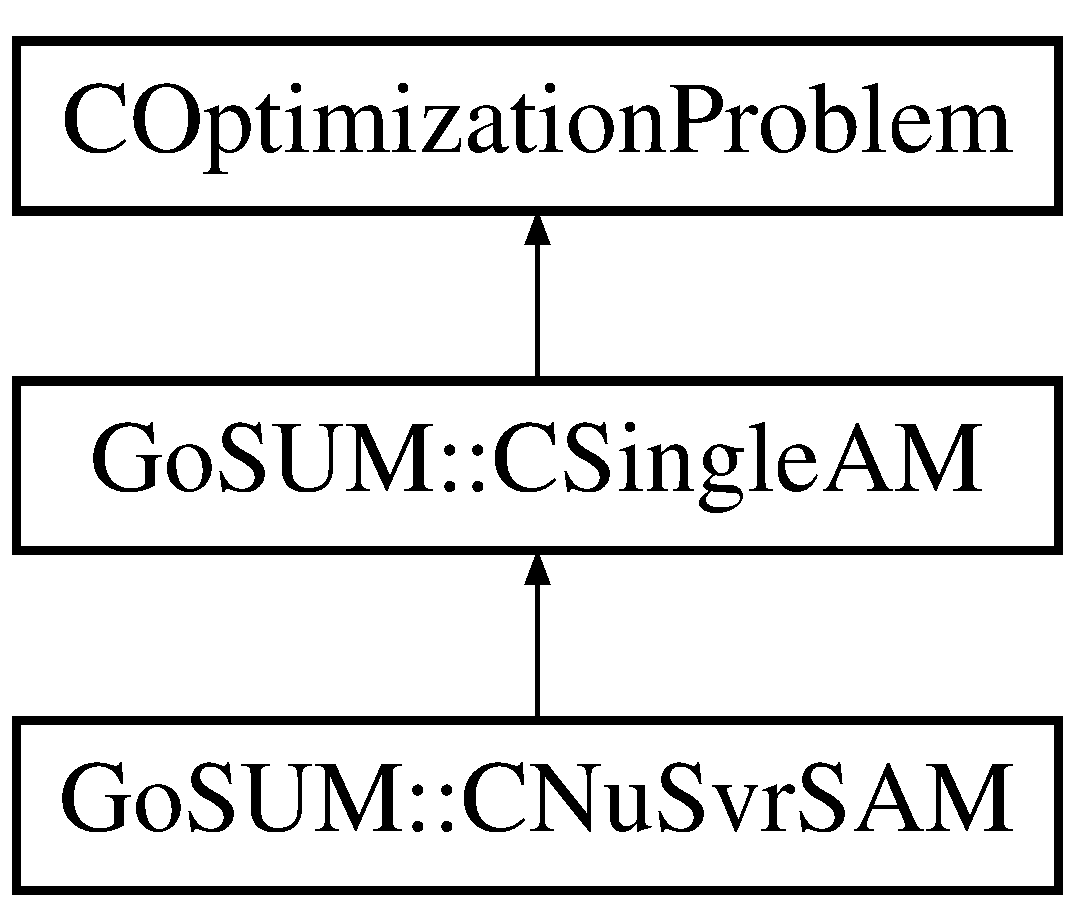
\includegraphics[height=3.000000cm]{class_go_s_u_m_1_1_c_nu_svr_s_a_m}
\end{center}
\end{figure}
\subsection*{Public Member Functions}
\begin{DoxyCompactItemize}
\item 
\hyperlink{class_go_s_u_m_1_1_c_nu_svr_s_a_m_acf81ebc1cc4dd607cec88bca0eceb8ac}{C\-Nu\-Svr\-S\-A\-M} ()
\item 
virtual \hyperlink{class_go_s_u_m_1_1_c_nu_svr_s_a_m_af8d6d8311722da418baa15b6f1d59f13}{$\sim$\-C\-Nu\-Svr\-S\-A\-M} ()
\item 
virtual void \hyperlink{class_go_s_u_m_1_1_c_nu_svr_s_a_m_a86f64a2aa6813481b3383eb0088efbbb}{open\-Optimization} ()
\begin{DoxyCompactList}\small\item\em Opens optmization. \end{DoxyCompactList}\item 
virtual void \hyperlink{class_go_s_u_m_1_1_c_nu_svr_s_a_m_aaa361789765b9862fb1ba2b04f0c24ac}{optimization\-Point2\-S\-V\-M\-Param} (const Array\-Xd \&ov)
\begin{DoxyCompactList}\small\item\em Converts optimization point to S\-V\-M parameters. \end{DoxyCompactList}\end{DoxyCompactItemize}
\subsection*{Protected Member Functions}
\begin{DoxyCompactItemize}
\item 
{\footnotesize template$<$class Archive $>$ }\\void \hyperlink{class_go_s_u_m_1_1_c_nu_svr_s_a_m_a5c67d2f1e31fc34fa5609f8d337afc6e}{serialize} (Archive \&ar, const unsigned int version)
\end{DoxyCompactItemize}
\subsection*{Friends}
\begin{DoxyCompactItemize}
\item 
class \hyperlink{class_go_s_u_m_1_1_c_nu_svr_s_a_m_ac98d07dd8f7b70e16ccb9a01abf56b9c}{boost\-::serialization\-::access}
\begin{DoxyCompactList}\small\item\em Boost serialization. \end{DoxyCompactList}\end{DoxyCompactItemize}
\subsection*{Additional Inherited Members}


\subsection{Detailed Description}
Class for the analyitical model for single output state, nu-\/\-S\-V\-R type. 

\subsection{Constructor \& Destructor Documentation}
\hypertarget{class_go_s_u_m_1_1_c_nu_svr_s_a_m_acf81ebc1cc4dd607cec88bca0eceb8ac}{\index{Go\-S\-U\-M\-::\-C\-Nu\-Svr\-S\-A\-M@{Go\-S\-U\-M\-::\-C\-Nu\-Svr\-S\-A\-M}!C\-Nu\-Svr\-S\-A\-M@{C\-Nu\-Svr\-S\-A\-M}}
\index{C\-Nu\-Svr\-S\-A\-M@{C\-Nu\-Svr\-S\-A\-M}!GoSUM::CNuSvrSAM@{Go\-S\-U\-M\-::\-C\-Nu\-Svr\-S\-A\-M}}
\subsubsection[{C\-Nu\-Svr\-S\-A\-M}]{\setlength{\rightskip}{0pt plus 5cm}Go\-S\-U\-M\-::\-C\-Nu\-Svr\-S\-A\-M\-::\-C\-Nu\-Svr\-S\-A\-M (
\begin{DoxyParamCaption}
{}
\end{DoxyParamCaption}
)\hspace{0.3cm}{\ttfamily [inline]}}}\label{class_go_s_u_m_1_1_c_nu_svr_s_a_m_acf81ebc1cc4dd607cec88bca0eceb8ac}
\hypertarget{class_go_s_u_m_1_1_c_nu_svr_s_a_m_af8d6d8311722da418baa15b6f1d59f13}{\index{Go\-S\-U\-M\-::\-C\-Nu\-Svr\-S\-A\-M@{Go\-S\-U\-M\-::\-C\-Nu\-Svr\-S\-A\-M}!$\sim$\-C\-Nu\-Svr\-S\-A\-M@{$\sim$\-C\-Nu\-Svr\-S\-A\-M}}
\index{$\sim$\-C\-Nu\-Svr\-S\-A\-M@{$\sim$\-C\-Nu\-Svr\-S\-A\-M}!GoSUM::CNuSvrSAM@{Go\-S\-U\-M\-::\-C\-Nu\-Svr\-S\-A\-M}}
\subsubsection[{$\sim$\-C\-Nu\-Svr\-S\-A\-M}]{\setlength{\rightskip}{0pt plus 5cm}virtual Go\-S\-U\-M\-::\-C\-Nu\-Svr\-S\-A\-M\-::$\sim$\-C\-Nu\-Svr\-S\-A\-M (
\begin{DoxyParamCaption}
{}
\end{DoxyParamCaption}
)\hspace{0.3cm}{\ttfamily [inline]}, {\ttfamily [virtual]}}}\label{class_go_s_u_m_1_1_c_nu_svr_s_a_m_af8d6d8311722da418baa15b6f1d59f13}


\subsection{Member Function Documentation}
\hypertarget{class_go_s_u_m_1_1_c_nu_svr_s_a_m_a86f64a2aa6813481b3383eb0088efbbb}{\index{Go\-S\-U\-M\-::\-C\-Nu\-Svr\-S\-A\-M@{Go\-S\-U\-M\-::\-C\-Nu\-Svr\-S\-A\-M}!open\-Optimization@{open\-Optimization}}
\index{open\-Optimization@{open\-Optimization}!GoSUM::CNuSvrSAM@{Go\-S\-U\-M\-::\-C\-Nu\-Svr\-S\-A\-M}}
\subsubsection[{open\-Optimization}]{\setlength{\rightskip}{0pt plus 5cm}void Go\-S\-U\-M\-::\-C\-Nu\-Svr\-S\-A\-M\-::open\-Optimization (
\begin{DoxyParamCaption}
{}
\end{DoxyParamCaption}
)\hspace{0.3cm}{\ttfamily [virtual]}}}\label{class_go_s_u_m_1_1_c_nu_svr_s_a_m_a86f64a2aa6813481b3383eb0088efbbb}


Opens optmization. 



Reimplemented from \hyperlink{class_go_s_u_m_1_1_c_single_a_m_acdaa489065049af967092e904004f299}{Go\-S\-U\-M\-::\-C\-Single\-A\-M}.

\hypertarget{class_go_s_u_m_1_1_c_nu_svr_s_a_m_aaa361789765b9862fb1ba2b04f0c24ac}{\index{Go\-S\-U\-M\-::\-C\-Nu\-Svr\-S\-A\-M@{Go\-S\-U\-M\-::\-C\-Nu\-Svr\-S\-A\-M}!optimization\-Point2\-S\-V\-M\-Param@{optimization\-Point2\-S\-V\-M\-Param}}
\index{optimization\-Point2\-S\-V\-M\-Param@{optimization\-Point2\-S\-V\-M\-Param}!GoSUM::CNuSvrSAM@{Go\-S\-U\-M\-::\-C\-Nu\-Svr\-S\-A\-M}}
\subsubsection[{optimization\-Point2\-S\-V\-M\-Param}]{\setlength{\rightskip}{0pt plus 5cm}void Go\-S\-U\-M\-::\-C\-Nu\-Svr\-S\-A\-M\-::optimization\-Point2\-S\-V\-M\-Param (
\begin{DoxyParamCaption}
\item[{const Array\-Xd \&}]{ov}
\end{DoxyParamCaption}
)\hspace{0.3cm}{\ttfamily [virtual]}}}\label{class_go_s_u_m_1_1_c_nu_svr_s_a_m_aaa361789765b9862fb1ba2b04f0c24ac}


Converts optimization point to S\-V\-M parameters. 



Reimplemented from \hyperlink{class_go_s_u_m_1_1_c_single_a_m_a28c4026a43409c73e27acbdabfff35ee}{Go\-S\-U\-M\-::\-C\-Single\-A\-M}.

\hypertarget{class_go_s_u_m_1_1_c_nu_svr_s_a_m_a5c67d2f1e31fc34fa5609f8d337afc6e}{\index{Go\-S\-U\-M\-::\-C\-Nu\-Svr\-S\-A\-M@{Go\-S\-U\-M\-::\-C\-Nu\-Svr\-S\-A\-M}!serialize@{serialize}}
\index{serialize@{serialize}!GoSUM::CNuSvrSAM@{Go\-S\-U\-M\-::\-C\-Nu\-Svr\-S\-A\-M}}
\subsubsection[{serialize}]{\setlength{\rightskip}{0pt plus 5cm}template$<$class Archive $>$ void Go\-S\-U\-M\-::\-C\-Nu\-Svr\-S\-A\-M\-::serialize (
\begin{DoxyParamCaption}
\item[{Archive \&}]{ar, }
\item[{const unsigned int}]{version}
\end{DoxyParamCaption}
)\hspace{0.3cm}{\ttfamily [protected]}}}\label{class_go_s_u_m_1_1_c_nu_svr_s_a_m_a5c67d2f1e31fc34fa5609f8d337afc6e}


Reimplemented from \hyperlink{class_go_s_u_m_1_1_c_single_a_m_a761e514fefeb7324e5509571f1be3848}{Go\-S\-U\-M\-::\-C\-Single\-A\-M}.



\subsection{Friends And Related Function Documentation}
\hypertarget{class_go_s_u_m_1_1_c_nu_svr_s_a_m_ac98d07dd8f7b70e16ccb9a01abf56b9c}{\index{Go\-S\-U\-M\-::\-C\-Nu\-Svr\-S\-A\-M@{Go\-S\-U\-M\-::\-C\-Nu\-Svr\-S\-A\-M}!boost\-::serialization\-::access@{boost\-::serialization\-::access}}
\index{boost\-::serialization\-::access@{boost\-::serialization\-::access}!GoSUM::CNuSvrSAM@{Go\-S\-U\-M\-::\-C\-Nu\-Svr\-S\-A\-M}}
\subsubsection[{boost\-::serialization\-::access}]{\setlength{\rightskip}{0pt plus 5cm}friend class boost\-::serialization\-::access\hspace{0.3cm}{\ttfamily [friend]}}}\label{class_go_s_u_m_1_1_c_nu_svr_s_a_m_ac98d07dd8f7b70e16ccb9a01abf56b9c}


Boost serialization. 



The documentation for this class was generated from the following files\-:\begin{DoxyCompactItemize}
\item 
C\-:/\-Development/core/\hyperlink{_analytical_model_8h}{Analytical\-Model.\-h}\item 
C\-:/\-Development/core/\hyperlink{_analytical_model_8cpp}{Analytical\-Model.\-cpp}\end{DoxyCompactItemize}

\hypertarget{class_go_s_u_m_1_1_c_one_class_s_a_m}{\section{Go\-S\-U\-M\-:\-:C\-One\-Class\-S\-A\-M Class Reference}
\label{class_go_s_u_m_1_1_c_one_class_s_a_m}\index{Go\-S\-U\-M\-::\-C\-One\-Class\-S\-A\-M@{Go\-S\-U\-M\-::\-C\-One\-Class\-S\-A\-M}}
}


Class for the analyitical model for single output state, one class type.  




{\ttfamily \#include $<$Analytical\-Model.\-h$>$}

Inheritance diagram for Go\-S\-U\-M\-:\-:C\-One\-Class\-S\-A\-M\-:\begin{figure}[H]
\begin{center}
\leavevmode
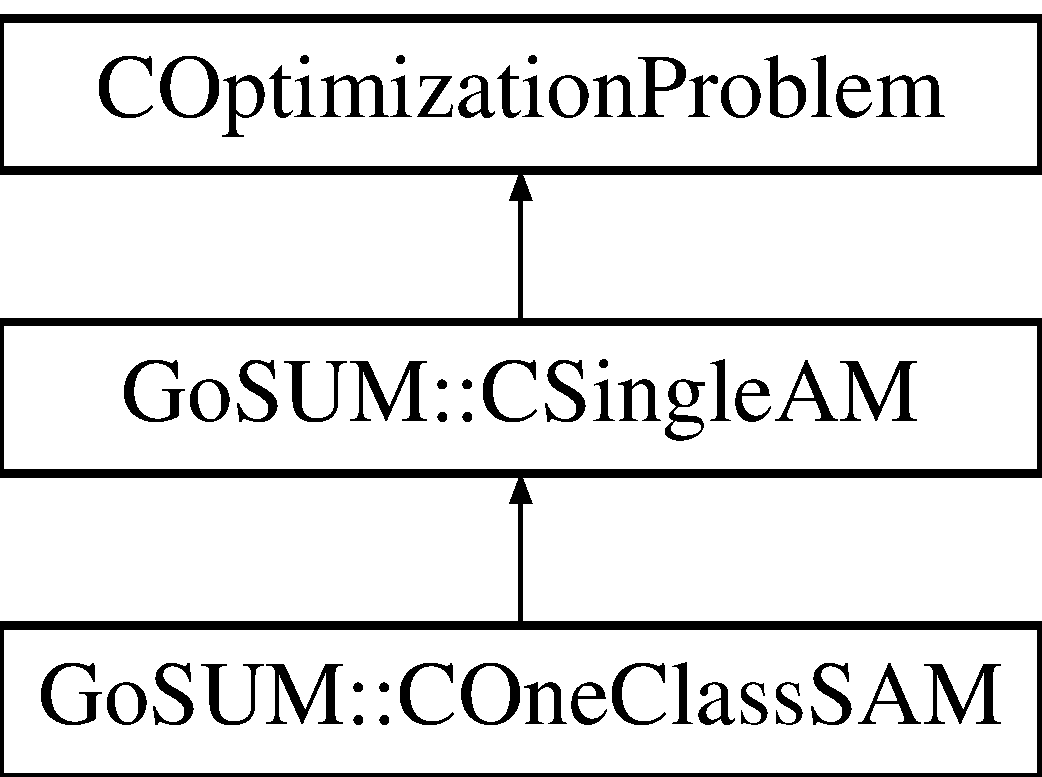
\includegraphics[height=3.000000cm]{class_go_s_u_m_1_1_c_one_class_s_a_m}
\end{center}
\end{figure}
\subsection*{Public Member Functions}
\begin{DoxyCompactItemize}
\item 
\hyperlink{class_go_s_u_m_1_1_c_one_class_s_a_m_a050f13fc2eb9e6f809bf1ed0183336ca}{C\-One\-Class\-S\-A\-M} ()
\item 
virtual \hyperlink{class_go_s_u_m_1_1_c_one_class_s_a_m_a5af7b14ea2a8cbbf347df65d4a583b5a}{$\sim$\-C\-One\-Class\-S\-A\-M} ()
\end{DoxyCompactItemize}
\subsection*{Protected Member Functions}
\begin{DoxyCompactItemize}
\item 
{\footnotesize template$<$class Archive $>$ }\\void \hyperlink{class_go_s_u_m_1_1_c_one_class_s_a_m_a68ab0232a5c0b2d978b356d05ad4b933}{serialize} (Archive \&ar, const unsigned int version)
\end{DoxyCompactItemize}
\subsection*{Friends}
\begin{DoxyCompactItemize}
\item 
class \hyperlink{class_go_s_u_m_1_1_c_one_class_s_a_m_ac98d07dd8f7b70e16ccb9a01abf56b9c}{boost\-::serialization\-::access}
\begin{DoxyCompactList}\small\item\em Boost serialization. \end{DoxyCompactList}\end{DoxyCompactItemize}
\subsection*{Additional Inherited Members}


\subsection{Detailed Description}
Class for the analyitical model for single output state, one class type. 

\subsection{Constructor \& Destructor Documentation}
\hypertarget{class_go_s_u_m_1_1_c_one_class_s_a_m_a050f13fc2eb9e6f809bf1ed0183336ca}{\index{Go\-S\-U\-M\-::\-C\-One\-Class\-S\-A\-M@{Go\-S\-U\-M\-::\-C\-One\-Class\-S\-A\-M}!C\-One\-Class\-S\-A\-M@{C\-One\-Class\-S\-A\-M}}
\index{C\-One\-Class\-S\-A\-M@{C\-One\-Class\-S\-A\-M}!GoSUM::COneClassSAM@{Go\-S\-U\-M\-::\-C\-One\-Class\-S\-A\-M}}
\subsubsection[{C\-One\-Class\-S\-A\-M}]{\setlength{\rightskip}{0pt plus 5cm}Go\-S\-U\-M\-::\-C\-One\-Class\-S\-A\-M\-::\-C\-One\-Class\-S\-A\-M (
\begin{DoxyParamCaption}
{}
\end{DoxyParamCaption}
)\hspace{0.3cm}{\ttfamily [inline]}}}\label{class_go_s_u_m_1_1_c_one_class_s_a_m_a050f13fc2eb9e6f809bf1ed0183336ca}
\hypertarget{class_go_s_u_m_1_1_c_one_class_s_a_m_a5af7b14ea2a8cbbf347df65d4a583b5a}{\index{Go\-S\-U\-M\-::\-C\-One\-Class\-S\-A\-M@{Go\-S\-U\-M\-::\-C\-One\-Class\-S\-A\-M}!$\sim$\-C\-One\-Class\-S\-A\-M@{$\sim$\-C\-One\-Class\-S\-A\-M}}
\index{$\sim$\-C\-One\-Class\-S\-A\-M@{$\sim$\-C\-One\-Class\-S\-A\-M}!GoSUM::COneClassSAM@{Go\-S\-U\-M\-::\-C\-One\-Class\-S\-A\-M}}
\subsubsection[{$\sim$\-C\-One\-Class\-S\-A\-M}]{\setlength{\rightskip}{0pt plus 5cm}virtual Go\-S\-U\-M\-::\-C\-One\-Class\-S\-A\-M\-::$\sim$\-C\-One\-Class\-S\-A\-M (
\begin{DoxyParamCaption}
{}
\end{DoxyParamCaption}
)\hspace{0.3cm}{\ttfamily [inline]}, {\ttfamily [virtual]}}}\label{class_go_s_u_m_1_1_c_one_class_s_a_m_a5af7b14ea2a8cbbf347df65d4a583b5a}


\subsection{Member Function Documentation}
\hypertarget{class_go_s_u_m_1_1_c_one_class_s_a_m_a68ab0232a5c0b2d978b356d05ad4b933}{\index{Go\-S\-U\-M\-::\-C\-One\-Class\-S\-A\-M@{Go\-S\-U\-M\-::\-C\-One\-Class\-S\-A\-M}!serialize@{serialize}}
\index{serialize@{serialize}!GoSUM::COneClassSAM@{Go\-S\-U\-M\-::\-C\-One\-Class\-S\-A\-M}}
\subsubsection[{serialize}]{\setlength{\rightskip}{0pt plus 5cm}template$<$class Archive $>$ void Go\-S\-U\-M\-::\-C\-One\-Class\-S\-A\-M\-::serialize (
\begin{DoxyParamCaption}
\item[{Archive \&}]{ar, }
\item[{const unsigned int}]{version}
\end{DoxyParamCaption}
)\hspace{0.3cm}{\ttfamily [protected]}}}\label{class_go_s_u_m_1_1_c_one_class_s_a_m_a68ab0232a5c0b2d978b356d05ad4b933}


Reimplemented from \hyperlink{class_go_s_u_m_1_1_c_single_a_m_a761e514fefeb7324e5509571f1be3848}{Go\-S\-U\-M\-::\-C\-Single\-A\-M}.



\subsection{Friends And Related Function Documentation}
\hypertarget{class_go_s_u_m_1_1_c_one_class_s_a_m_ac98d07dd8f7b70e16ccb9a01abf56b9c}{\index{Go\-S\-U\-M\-::\-C\-One\-Class\-S\-A\-M@{Go\-S\-U\-M\-::\-C\-One\-Class\-S\-A\-M}!boost\-::serialization\-::access@{boost\-::serialization\-::access}}
\index{boost\-::serialization\-::access@{boost\-::serialization\-::access}!GoSUM::COneClassSAM@{Go\-S\-U\-M\-::\-C\-One\-Class\-S\-A\-M}}
\subsubsection[{boost\-::serialization\-::access}]{\setlength{\rightskip}{0pt plus 5cm}friend class boost\-::serialization\-::access\hspace{0.3cm}{\ttfamily [friend]}}}\label{class_go_s_u_m_1_1_c_one_class_s_a_m_ac98d07dd8f7b70e16ccb9a01abf56b9c}


Boost serialization. 



The documentation for this class was generated from the following files\-:\begin{DoxyCompactItemize}
\item 
C\-:/\-Development/core/\hyperlink{_analytical_model_8h}{Analytical\-Model.\-h}\item 
C\-:/\-Development/core/\hyperlink{_analytical_model_8cpp}{Analytical\-Model.\-cpp}\end{DoxyCompactItemize}

\hypertarget{class_c_optimization_problem}{\section{C\-Optimization\-Problem Class Reference}
\label{class_c_optimization_problem}\index{C\-Optimization\-Problem@{C\-Optimization\-Problem}}
}


Class for the optimization problem.  




{\ttfamily \#include $<$Optimization\-Problem.\-h$>$}

Inheritance diagram for C\-Optimization\-Problem\-:\begin{figure}[H]
\begin{center}
\leavevmode
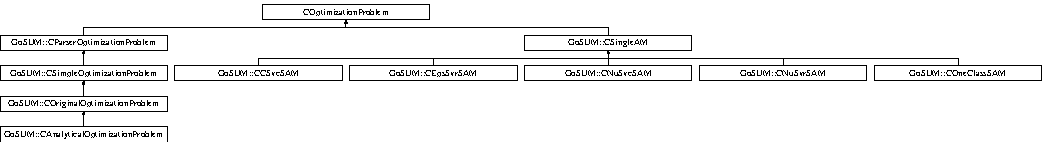
\includegraphics[height=1.881720cm]{class_c_optimization_problem}
\end{center}
\end{figure}
\subsection*{Public Member Functions}
\begin{DoxyCompactItemize}
\item 
\hyperlink{class_c_optimization_problem_aa0a4b0429250454fdf87722ed36d98d5}{C\-Optimization\-Problem} ()
\item 
virtual \hyperlink{class_c_optimization_problem_afd552fd41afa6355dd5e1d8b72b79739}{$\sim$\-C\-Optimization\-Problem} ()
\item 
virtual void \hyperlink{class_c_optimization_problem_a59a36304309b79f0dc7be25638016ee0}{clear} ()
\begin{DoxyCompactList}\small\item\em Clears all. \end{DoxyCompactList}\item 
virtual void \hyperlink{class_c_optimization_problem_a405d5e1e0008ba9e8604327632e93cbe}{clear\-History} ()
\begin{DoxyCompactList}\small\item\em Clears results. \end{DoxyCompactList}\item 
bool \hyperlink{class_c_optimization_problem_a9b2dfd8207421acd7e51b45d4d512400}{empty\-History} () const 
\begin{DoxyCompactList}\small\item\em Returns true if results are empty. false otherwise. \end{DoxyCompactList}\item 
bool \hyperlink{class_c_optimization_problem_a6e087d18a2bafd52881272c07be0b030}{is\-Minimization} ()
\begin{DoxyCompactList}\small\item\em Returns true if it is a minimization problem, false otherwise. \end{DoxyCompactList}\item 
bool \hyperlink{class_c_optimization_problem_a1986507efbe70517b0f4fb470f80558a}{is\-Maximization} ()
\begin{DoxyCompactList}\small\item\em Returns true if it is a maximization problem, false otherwise. \end{DoxyCompactList}\item 
void \hyperlink{class_c_optimization_problem_a165b7a6584eb085ae51edae5f7dbca13}{set\-Minimization} ()
\begin{DoxyCompactList}\small\item\em Sets optimization problem to minimization. \end{DoxyCompactList}\item 
void \hyperlink{class_c_optimization_problem_a20b7943d855d629bdfcf111e0ff534b6}{set\-Maximization} ()
\begin{DoxyCompactList}\small\item\em Sets optimization problem to maximization. \end{DoxyCompactList}\item 
int \hyperlink{class_c_optimization_problem_a5390a1e20ac8312e02f5de27fc575bdd}{dimension} () const 
\begin{DoxyCompactList}\small\item\em Returns dimension of the problem. \end{DoxyCompactList}\item 
\hyperlink{class_c_optimization_variable}{C\-Optimization\-Variable} $\ast$ \hyperlink{class_c_optimization_problem_adff750a5b896e95a8328627110b66da7}{add\-Variable} (\hyperlink{class_c_optimization_variable}{C\-Optimization\-Variable} $\ast$\-\_\-p\-O\-V)
\begin{DoxyCompactList}\small\item\em Adds optimization variable. \end{DoxyCompactList}\item 
void \hyperlink{class_c_optimization_problem_a7f18cd310761a871d13c914ea803e75a}{erase\-Variable} (int \-\_\-at)
\begin{DoxyCompactList}\small\item\em Erases particular optimization variable. \end{DoxyCompactList}\item 
void \hyperlink{class_c_optimization_problem_acb9cf75e7dcce19ddde928f73ee2a6dd}{set\-Lower\-Bound} (const Array\-Xd \&\-\_\-x\-L)
\begin{DoxyCompactList}\small\item\em Sets lower bound of the optimization variables. \end{DoxyCompactList}\item 
void \hyperlink{class_c_optimization_problem_a7fc1c240a370dd6f534d9feac9400581}{set\-Upper\-Bound} (const Array\-Xd \&\-\_\-x\-U)
\begin{DoxyCompactList}\small\item\em Sets upper bound of the optimization variables. \end{DoxyCompactList}\item 
void \hyperlink{class_c_optimization_problem_a181f9b453ce641a6eb08f0fee1025bd1}{set\-Initial\-Value} (const Array\-Xd \&\-\_\-x0)
\begin{DoxyCompactList}\small\item\em Sets initial value of the optimization variables. \end{DoxyCompactList}\item 
Array\-Xd \hyperlink{class_c_optimization_problem_a43bb9bd0b393b5dc790967f6019fefc9}{lower\-Bound} () const 
\begin{DoxyCompactList}\small\item\em Returns lower bound of the optimization variables. \end{DoxyCompactList}\item 
Array\-Xd \hyperlink{class_c_optimization_problem_a309631e1082dd7508bbf24cfd6eb8b4b}{upper\-Bound} () const 
\begin{DoxyCompactList}\small\item\em returns upper bound of the optimization variables. \end{DoxyCompactList}\item 
Array\-Xd \hyperlink{class_c_optimization_problem_a1b52c22548bb9057675d343a3ac3cbb4}{initial\-Value} () const 
\begin{DoxyCompactList}\small\item\em Returns initial value of the optimization variables. \end{DoxyCompactList}\item 
void \hyperlink{class_c_optimization_problem_a91430a451c3c8a63ebc9557165a2180e}{set\-Lower\-Bound} (int \-\_\-at, double \-\_\-x\-L)
\begin{DoxyCompactList}\small\item\em Sets lower bound of the optimization variables. \end{DoxyCompactList}\item 
void \hyperlink{class_c_optimization_problem_a310b6d74b2cc7f276185726d7346158b}{set\-Upper\-Bound} (int \-\_\-at, double \-\_\-x\-U)
\begin{DoxyCompactList}\small\item\em Sets upper bound of the optimization variables. \end{DoxyCompactList}\item 
void \hyperlink{class_c_optimization_problem_a96a8e72816d8234cc84504bcbcabdb5a}{set\-Initial\-Value} (int \-\_\-at, double \-\_\-x0)
\begin{DoxyCompactList}\small\item\em Sets initial value of the optimization variables. \end{DoxyCompactList}\item 
double \hyperlink{class_c_optimization_problem_a0efb201cd766f922fb2b7da2e45aa5e7}{lower\-Bound} (int \-\_\-at) const 
\begin{DoxyCompactList}\small\item\em Returns lower bound of the optimization variables. \end{DoxyCompactList}\item 
double \hyperlink{class_c_optimization_problem_a389f3d72ef773631e96d42b152d2bb2e}{upper\-Bound} (int \-\_\-at) const 
\begin{DoxyCompactList}\small\item\em Returns upper bound of the optimization variables. \end{DoxyCompactList}\item 
double \hyperlink{class_c_optimization_problem_ae1fc23613ecf4730353102bf9132fddb}{initial\-Value} (int \-\_\-at) const 
\begin{DoxyCompactList}\small\item\em Returns initial value of the optimization variables. \end{DoxyCompactList}\item 
virtual double \hyperlink{class_c_optimization_problem_a3e0cc82f344895bd593d1960c4fbadf9}{objective} (const Array\-Xd \&\-\_\-ov)=0
\begin{DoxyCompactList}\small\item\em Evaluates objective function value from optimization variables values. \end{DoxyCompactList}\item 
virtual bool \hyperlink{class_c_optimization_problem_ad3bfb3d51edfeeb18be3ce32731c2ed1}{is\-Feasible} (const Array\-Xd \&\-\_\-ov)
\begin{DoxyCompactList}\small\item\em Returns true if optimization variable is feasible, false otherwise. \end{DoxyCompactList}\item 
virtual int \hyperlink{class_c_optimization_problem_aa4c04d9a7d3885450e9c528f5446c241}{constraints\-Size} () const =0
\begin{DoxyCompactList}\small\item\em Returns size of the constraints. \end{DoxyCompactList}\item 
virtual double \hyperlink{class_c_optimization_problem_ac37dd6a981b9049943189b3fea343f64}{constraint} (const Array\-Xd \&\-\_\-ov, int \-\_\-at)=0
\begin{DoxyCompactList}\small\item\em Evalautes particular constraint value from optimization variables values. \end{DoxyCompactList}\item 
virtual bool \hyperlink{class_c_optimization_problem_a6edffc27d4d909c9572a95d7ea6c7c8b}{evaluate} (const Array\-Xd \&\-\_\-hp, Array\-Xd \&\-\_\-ep)
\begin{DoxyCompactList}\small\item\em Evaluates objective and all constraints from optimization variables values and returns true if it is feasible, false otherwise. \end{DoxyCompactList}\item 
virtual void \hyperlink{class_c_optimization_problem_af06324e65035961b500de11edcdab889}{open\-Optimization} ()
\item 
virtual void \hyperlink{class_c_optimization_problem_a30fa53ab400882df886d28109ed92ea1}{close\-Optimization} ()
\begin{DoxyCompactList}\small\item\em Opens, i.\-e. prepares optimization. \end{DoxyCompactList}\item 
void \hyperlink{class_c_optimization_problem_a36a9c34a0e2a09929d2fc05839836603}{write\-History} (const Array\-Xd \&\-\_\-ov, double \-\_\-res)
\begin{DoxyCompactList}\small\item\em Closes optimization, i.\-e. closes what was opened in open\-Optimization. \end{DoxyCompactList}\item 
int \hyperlink{class_c_optimization_problem_ae1aa05b9f3328cf2dc77a29ad120ec22}{history\-Size} () const 
\begin{DoxyCompactList}\small\item\em Returns history size. \end{DoxyCompactList}\item 
double \hyperlink{class_c_optimization_problem_a54e11507c7aeb08e8b5dfadafb285ab7}{objective\-History} (int \-\_\-i) const 
\begin{DoxyCompactList}\small\item\em Returns particular objective history. \end{DoxyCompactList}\item 
double \hyperlink{class_c_optimization_problem_a0bcf4f49c2bb0e5f9aad9fa33a26bdc6}{variable\-History} (int \-\_\-i, int \-\_\-j) const 
\begin{DoxyCompactList}\small\item\em Returns particular variable history. \end{DoxyCompactList}\item 
Array\-Xd \hyperlink{class_c_optimization_problem_a318e826a400755d4c15852af1fb2962c}{export\-Objective\-History} () const 
\begin{DoxyCompactList}\small\item\em Exports objective history. \end{DoxyCompactList}\end{DoxyCompactItemize}
\subsection*{Protected Member Functions}
\begin{DoxyCompactItemize}
\item 
{\footnotesize template$<$class Archive $>$ }\\void \hyperlink{class_c_optimization_problem_ad5b8db9e394c4eedeb28686acb4dce43}{serialize} (Archive \&ar, const unsigned int version)
\end{DoxyCompactItemize}
\subsection*{Protected Attributes}
\begin{DoxyCompactItemize}
\item 
bool \hyperlink{class_c_optimization_problem_a142569515a786cf11c7ec6337e9aca61}{minimize}
\begin{DoxyCompactList}\small\item\em Indicates if it is a minimization problem. \end{DoxyCompactList}\item 
boost\-::ptr\-\_\-vector\\*
$<$ \hyperlink{class_c_optimization_variable}{C\-Optimization\-Variable} $>$ \hyperlink{class_c_optimization_problem_a42fa0c335f002a47acab9e846bbc13ea}{ovs}
\begin{DoxyCompactList}\small\item\em Holds all optimization variables. \end{DoxyCompactList}\item 
std\-::vector$<$ std\-::pair\\*
$<$ Array\-Xd, double $>$ $>$ \hyperlink{class_c_optimization_problem_a86bb928e976091481a4f26db15a67ff5}{history}
\end{DoxyCompactItemize}
\subsection*{Friends}
\begin{DoxyCompactItemize}
\item 
class \hyperlink{class_c_optimization_problem_ac98d07dd8f7b70e16ccb9a01abf56b9c}{boost\-::serialization\-::access}
\begin{DoxyCompactList}\small\item\em Boost serialization. \end{DoxyCompactList}\end{DoxyCompactItemize}


\subsection{Detailed Description}
Class for the optimization problem. 

\subsection{Constructor \& Destructor Documentation}
\hypertarget{class_c_optimization_problem_aa0a4b0429250454fdf87722ed36d98d5}{\index{C\-Optimization\-Problem@{C\-Optimization\-Problem}!C\-Optimization\-Problem@{C\-Optimization\-Problem}}
\index{C\-Optimization\-Problem@{C\-Optimization\-Problem}!COptimizationProblem@{C\-Optimization\-Problem}}
\subsubsection[{C\-Optimization\-Problem}]{\setlength{\rightskip}{0pt plus 5cm}C\-Optimization\-Problem\-::\-C\-Optimization\-Problem (
\begin{DoxyParamCaption}
{}
\end{DoxyParamCaption}
)\hspace{0.3cm}{\ttfamily [inline]}}}\label{class_c_optimization_problem_aa0a4b0429250454fdf87722ed36d98d5}
\hypertarget{class_c_optimization_problem_afd552fd41afa6355dd5e1d8b72b79739}{\index{C\-Optimization\-Problem@{C\-Optimization\-Problem}!$\sim$\-C\-Optimization\-Problem@{$\sim$\-C\-Optimization\-Problem}}
\index{$\sim$\-C\-Optimization\-Problem@{$\sim$\-C\-Optimization\-Problem}!COptimizationProblem@{C\-Optimization\-Problem}}
\subsubsection[{$\sim$\-C\-Optimization\-Problem}]{\setlength{\rightskip}{0pt plus 5cm}virtual C\-Optimization\-Problem\-::$\sim$\-C\-Optimization\-Problem (
\begin{DoxyParamCaption}
{}
\end{DoxyParamCaption}
)\hspace{0.3cm}{\ttfamily [inline]}, {\ttfamily [virtual]}}}\label{class_c_optimization_problem_afd552fd41afa6355dd5e1d8b72b79739}


\subsection{Member Function Documentation}
\hypertarget{class_c_optimization_problem_adff750a5b896e95a8328627110b66da7}{\index{C\-Optimization\-Problem@{C\-Optimization\-Problem}!add\-Variable@{add\-Variable}}
\index{add\-Variable@{add\-Variable}!COptimizationProblem@{C\-Optimization\-Problem}}
\subsubsection[{add\-Variable}]{\setlength{\rightskip}{0pt plus 5cm}{\bf C\-Optimization\-Variable}$\ast$ C\-Optimization\-Problem\-::add\-Variable (
\begin{DoxyParamCaption}
\item[{{\bf C\-Optimization\-Variable} $\ast$}]{\-\_\-p\-O\-V}
\end{DoxyParamCaption}
)\hspace{0.3cm}{\ttfamily [inline]}}}\label{class_c_optimization_problem_adff750a5b896e95a8328627110b66da7}


Adds optimization variable. 

\hypertarget{class_c_optimization_problem_a59a36304309b79f0dc7be25638016ee0}{\index{C\-Optimization\-Problem@{C\-Optimization\-Problem}!clear@{clear}}
\index{clear@{clear}!COptimizationProblem@{C\-Optimization\-Problem}}
\subsubsection[{clear}]{\setlength{\rightskip}{0pt plus 5cm}virtual void C\-Optimization\-Problem\-::clear (
\begin{DoxyParamCaption}
{}
\end{DoxyParamCaption}
)\hspace{0.3cm}{\ttfamily [inline]}, {\ttfamily [virtual]}}}\label{class_c_optimization_problem_a59a36304309b79f0dc7be25638016ee0}


Clears all. 



Reimplemented in \hyperlink{class_go_s_u_m_1_1_c_simple_optimization_problem_ac5843023c605a273e8276656336b51af}{Go\-S\-U\-M\-::\-C\-Simple\-Optimization\-Problem}.

\hypertarget{class_c_optimization_problem_a405d5e1e0008ba9e8604327632e93cbe}{\index{C\-Optimization\-Problem@{C\-Optimization\-Problem}!clear\-History@{clear\-History}}
\index{clear\-History@{clear\-History}!COptimizationProblem@{C\-Optimization\-Problem}}
\subsubsection[{clear\-History}]{\setlength{\rightskip}{0pt plus 5cm}virtual void C\-Optimization\-Problem\-::clear\-History (
\begin{DoxyParamCaption}
{}
\end{DoxyParamCaption}
)\hspace{0.3cm}{\ttfamily [inline]}, {\ttfamily [virtual]}}}\label{class_c_optimization_problem_a405d5e1e0008ba9e8604327632e93cbe}


Clears results. 



Reimplemented in \hyperlink{class_go_s_u_m_1_1_c_simple_optimization_problem_a87a5cfb79c799788b85705794c373f40}{Go\-S\-U\-M\-::\-C\-Simple\-Optimization\-Problem}.

\hypertarget{class_c_optimization_problem_a30fa53ab400882df886d28109ed92ea1}{\index{C\-Optimization\-Problem@{C\-Optimization\-Problem}!close\-Optimization@{close\-Optimization}}
\index{close\-Optimization@{close\-Optimization}!COptimizationProblem@{C\-Optimization\-Problem}}
\subsubsection[{close\-Optimization}]{\setlength{\rightskip}{0pt plus 5cm}virtual void C\-Optimization\-Problem\-::close\-Optimization (
\begin{DoxyParamCaption}
{}
\end{DoxyParamCaption}
)\hspace{0.3cm}{\ttfamily [inline]}, {\ttfamily [virtual]}}}\label{class_c_optimization_problem_a30fa53ab400882df886d28109ed92ea1}


Opens, i.\-e. prepares optimization. 



Reimplemented in \hyperlink{class_go_s_u_m_1_1_c_original_optimization_problem_a75b28528cda5b1be7bdc2cc4a309a314}{Go\-S\-U\-M\-::\-C\-Original\-Optimization\-Problem}, \hyperlink{class_go_s_u_m_1_1_c_simple_optimization_problem_af34b88f099f94727611b79d5f5ca4e9a}{Go\-S\-U\-M\-::\-C\-Simple\-Optimization\-Problem}, and \hyperlink{class_go_s_u_m_1_1_c_parser_optimization_problem_aa750bd3725ca5e71d8ce9901e78661a8}{Go\-S\-U\-M\-::\-C\-Parser\-Optimization\-Problem}.

\hypertarget{class_c_optimization_problem_ac37dd6a981b9049943189b3fea343f64}{\index{C\-Optimization\-Problem@{C\-Optimization\-Problem}!constraint@{constraint}}
\index{constraint@{constraint}!COptimizationProblem@{C\-Optimization\-Problem}}
\subsubsection[{constraint}]{\setlength{\rightskip}{0pt plus 5cm}virtual double C\-Optimization\-Problem\-::constraint (
\begin{DoxyParamCaption}
\item[{const Array\-Xd \&}]{\-\_\-ov, }
\item[{int}]{\-\_\-at}
\end{DoxyParamCaption}
)\hspace{0.3cm}{\ttfamily [pure virtual]}}}\label{class_c_optimization_problem_ac37dd6a981b9049943189b3fea343f64}


Evalautes particular constraint value from optimization variables values. 



Implemented in \hyperlink{class_go_s_u_m_1_1_c_single_a_m_ab45bdd4b3d7b5cab88e05ed6cd98e7e6}{Go\-S\-U\-M\-::\-C\-Single\-A\-M}, and \hyperlink{class_go_s_u_m_1_1_c_parser_optimization_problem_a90d550681fe3ef512822cfa9598eb5b0}{Go\-S\-U\-M\-::\-C\-Parser\-Optimization\-Problem}.

\hypertarget{class_c_optimization_problem_aa4c04d9a7d3885450e9c528f5446c241}{\index{C\-Optimization\-Problem@{C\-Optimization\-Problem}!constraints\-Size@{constraints\-Size}}
\index{constraints\-Size@{constraints\-Size}!COptimizationProblem@{C\-Optimization\-Problem}}
\subsubsection[{constraints\-Size}]{\setlength{\rightskip}{0pt plus 5cm}virtual int C\-Optimization\-Problem\-::constraints\-Size (
\begin{DoxyParamCaption}
{}
\end{DoxyParamCaption}
) const\hspace{0.3cm}{\ttfamily [pure virtual]}}}\label{class_c_optimization_problem_aa4c04d9a7d3885450e9c528f5446c241}


Returns size of the constraints. 



Implemented in \hyperlink{class_go_s_u_m_1_1_c_single_a_m_a77486d18726fc335328dd02bc676f74e}{Go\-S\-U\-M\-::\-C\-Single\-A\-M}, and \hyperlink{class_go_s_u_m_1_1_c_parser_optimization_problem_a038c506b870e9e77f7fd50b6f9864dcb}{Go\-S\-U\-M\-::\-C\-Parser\-Optimization\-Problem}.

\hypertarget{class_c_optimization_problem_a5390a1e20ac8312e02f5de27fc575bdd}{\index{C\-Optimization\-Problem@{C\-Optimization\-Problem}!dimension@{dimension}}
\index{dimension@{dimension}!COptimizationProblem@{C\-Optimization\-Problem}}
\subsubsection[{dimension}]{\setlength{\rightskip}{0pt plus 5cm}int C\-Optimization\-Problem\-::dimension (
\begin{DoxyParamCaption}
{}
\end{DoxyParamCaption}
) const\hspace{0.3cm}{\ttfamily [inline]}}}\label{class_c_optimization_problem_a5390a1e20ac8312e02f5de27fc575bdd}


Returns dimension of the problem. 

\hypertarget{class_c_optimization_problem_a9b2dfd8207421acd7e51b45d4d512400}{\index{C\-Optimization\-Problem@{C\-Optimization\-Problem}!empty\-History@{empty\-History}}
\index{empty\-History@{empty\-History}!COptimizationProblem@{C\-Optimization\-Problem}}
\subsubsection[{empty\-History}]{\setlength{\rightskip}{0pt plus 5cm}bool C\-Optimization\-Problem\-::empty\-History (
\begin{DoxyParamCaption}
{}
\end{DoxyParamCaption}
) const\hspace{0.3cm}{\ttfamily [inline]}}}\label{class_c_optimization_problem_a9b2dfd8207421acd7e51b45d4d512400}


Returns true if results are empty. false otherwise. 

\hypertarget{class_c_optimization_problem_a7f18cd310761a871d13c914ea803e75a}{\index{C\-Optimization\-Problem@{C\-Optimization\-Problem}!erase\-Variable@{erase\-Variable}}
\index{erase\-Variable@{erase\-Variable}!COptimizationProblem@{C\-Optimization\-Problem}}
\subsubsection[{erase\-Variable}]{\setlength{\rightskip}{0pt plus 5cm}void C\-Optimization\-Problem\-::erase\-Variable (
\begin{DoxyParamCaption}
\item[{int}]{\-\_\-at}
\end{DoxyParamCaption}
)}}\label{class_c_optimization_problem_a7f18cd310761a871d13c914ea803e75a}


Erases particular optimization variable. 

\hypertarget{class_c_optimization_problem_a6edffc27d4d909c9572a95d7ea6c7c8b}{\index{C\-Optimization\-Problem@{C\-Optimization\-Problem}!evaluate@{evaluate}}
\index{evaluate@{evaluate}!COptimizationProblem@{C\-Optimization\-Problem}}
\subsubsection[{evaluate}]{\setlength{\rightskip}{0pt plus 5cm}bool C\-Optimization\-Problem\-::evaluate (
\begin{DoxyParamCaption}
\item[{const Array\-Xd \&}]{\-\_\-hp, }
\item[{Array\-Xd \&}]{\-\_\-ep}
\end{DoxyParamCaption}
)\hspace{0.3cm}{\ttfamily [virtual]}}}\label{class_c_optimization_problem_a6edffc27d4d909c9572a95d7ea6c7c8b}


Evaluates objective and all constraints from optimization variables values and returns true if it is feasible, false otherwise. 



Reimplemented in \hyperlink{class_go_s_u_m_1_1_c_simple_optimization_problem_aa746b5adb39e80712ecddf18e466f4ab}{Go\-S\-U\-M\-::\-C\-Simple\-Optimization\-Problem}.

\hypertarget{class_c_optimization_problem_a318e826a400755d4c15852af1fb2962c}{\index{C\-Optimization\-Problem@{C\-Optimization\-Problem}!export\-Objective\-History@{export\-Objective\-History}}
\index{export\-Objective\-History@{export\-Objective\-History}!COptimizationProblem@{C\-Optimization\-Problem}}
\subsubsection[{export\-Objective\-History}]{\setlength{\rightskip}{0pt plus 5cm}Array\-Xd C\-Optimization\-Problem\-::export\-Objective\-History (
\begin{DoxyParamCaption}
{}
\end{DoxyParamCaption}
) const}}\label{class_c_optimization_problem_a318e826a400755d4c15852af1fb2962c}


Exports objective history. 

\hypertarget{class_c_optimization_problem_ae1aa05b9f3328cf2dc77a29ad120ec22}{\index{C\-Optimization\-Problem@{C\-Optimization\-Problem}!history\-Size@{history\-Size}}
\index{history\-Size@{history\-Size}!COptimizationProblem@{C\-Optimization\-Problem}}
\subsubsection[{history\-Size}]{\setlength{\rightskip}{0pt plus 5cm}int C\-Optimization\-Problem\-::history\-Size (
\begin{DoxyParamCaption}
{}
\end{DoxyParamCaption}
) const\hspace{0.3cm}{\ttfamily [inline]}}}\label{class_c_optimization_problem_ae1aa05b9f3328cf2dc77a29ad120ec22}


Returns history size. 

\hypertarget{class_c_optimization_problem_a1b52c22548bb9057675d343a3ac3cbb4}{\index{C\-Optimization\-Problem@{C\-Optimization\-Problem}!initial\-Value@{initial\-Value}}
\index{initial\-Value@{initial\-Value}!COptimizationProblem@{C\-Optimization\-Problem}}
\subsubsection[{initial\-Value}]{\setlength{\rightskip}{0pt plus 5cm}Array\-Xd C\-Optimization\-Problem\-::initial\-Value (
\begin{DoxyParamCaption}
{}
\end{DoxyParamCaption}
) const}}\label{class_c_optimization_problem_a1b52c22548bb9057675d343a3ac3cbb4}


Returns initial value of the optimization variables. 

\hypertarget{class_c_optimization_problem_ae1fc23613ecf4730353102bf9132fddb}{\index{C\-Optimization\-Problem@{C\-Optimization\-Problem}!initial\-Value@{initial\-Value}}
\index{initial\-Value@{initial\-Value}!COptimizationProblem@{C\-Optimization\-Problem}}
\subsubsection[{initial\-Value}]{\setlength{\rightskip}{0pt plus 5cm}double C\-Optimization\-Problem\-::initial\-Value (
\begin{DoxyParamCaption}
\item[{int}]{\-\_\-at}
\end{DoxyParamCaption}
) const\hspace{0.3cm}{\ttfamily [inline]}}}\label{class_c_optimization_problem_ae1fc23613ecf4730353102bf9132fddb}


Returns initial value of the optimization variables. 

\hypertarget{class_c_optimization_problem_ad3bfb3d51edfeeb18be3ce32731c2ed1}{\index{C\-Optimization\-Problem@{C\-Optimization\-Problem}!is\-Feasible@{is\-Feasible}}
\index{is\-Feasible@{is\-Feasible}!COptimizationProblem@{C\-Optimization\-Problem}}
\subsubsection[{is\-Feasible}]{\setlength{\rightskip}{0pt plus 5cm}virtual bool C\-Optimization\-Problem\-::is\-Feasible (
\begin{DoxyParamCaption}
\item[{const Array\-Xd \&}]{\-\_\-ov}
\end{DoxyParamCaption}
)\hspace{0.3cm}{\ttfamily [inline]}, {\ttfamily [virtual]}}}\label{class_c_optimization_problem_ad3bfb3d51edfeeb18be3ce32731c2ed1}


Returns true if optimization variable is feasible, false otherwise. 



Reimplemented in \hyperlink{class_go_s_u_m_1_1_c_simple_optimization_problem_aa66a0dd530b4cab400fc88b32f566298}{Go\-S\-U\-M\-::\-C\-Simple\-Optimization\-Problem}.

\hypertarget{class_c_optimization_problem_a1986507efbe70517b0f4fb470f80558a}{\index{C\-Optimization\-Problem@{C\-Optimization\-Problem}!is\-Maximization@{is\-Maximization}}
\index{is\-Maximization@{is\-Maximization}!COptimizationProblem@{C\-Optimization\-Problem}}
\subsubsection[{is\-Maximization}]{\setlength{\rightskip}{0pt plus 5cm}bool C\-Optimization\-Problem\-::is\-Maximization (
\begin{DoxyParamCaption}
{}
\end{DoxyParamCaption}
)\hspace{0.3cm}{\ttfamily [inline]}}}\label{class_c_optimization_problem_a1986507efbe70517b0f4fb470f80558a}


Returns true if it is a maximization problem, false otherwise. 

\hypertarget{class_c_optimization_problem_a6e087d18a2bafd52881272c07be0b030}{\index{C\-Optimization\-Problem@{C\-Optimization\-Problem}!is\-Minimization@{is\-Minimization}}
\index{is\-Minimization@{is\-Minimization}!COptimizationProblem@{C\-Optimization\-Problem}}
\subsubsection[{is\-Minimization}]{\setlength{\rightskip}{0pt plus 5cm}bool C\-Optimization\-Problem\-::is\-Minimization (
\begin{DoxyParamCaption}
{}
\end{DoxyParamCaption}
)\hspace{0.3cm}{\ttfamily [inline]}}}\label{class_c_optimization_problem_a6e087d18a2bafd52881272c07be0b030}


Returns true if it is a minimization problem, false otherwise. 

\hypertarget{class_c_optimization_problem_a43bb9bd0b393b5dc790967f6019fefc9}{\index{C\-Optimization\-Problem@{C\-Optimization\-Problem}!lower\-Bound@{lower\-Bound}}
\index{lower\-Bound@{lower\-Bound}!COptimizationProblem@{C\-Optimization\-Problem}}
\subsubsection[{lower\-Bound}]{\setlength{\rightskip}{0pt plus 5cm}Array\-Xd C\-Optimization\-Problem\-::lower\-Bound (
\begin{DoxyParamCaption}
{}
\end{DoxyParamCaption}
) const}}\label{class_c_optimization_problem_a43bb9bd0b393b5dc790967f6019fefc9}


Returns lower bound of the optimization variables. 

\hypertarget{class_c_optimization_problem_a0efb201cd766f922fb2b7da2e45aa5e7}{\index{C\-Optimization\-Problem@{C\-Optimization\-Problem}!lower\-Bound@{lower\-Bound}}
\index{lower\-Bound@{lower\-Bound}!COptimizationProblem@{C\-Optimization\-Problem}}
\subsubsection[{lower\-Bound}]{\setlength{\rightskip}{0pt plus 5cm}double C\-Optimization\-Problem\-::lower\-Bound (
\begin{DoxyParamCaption}
\item[{int}]{\-\_\-at}
\end{DoxyParamCaption}
) const\hspace{0.3cm}{\ttfamily [inline]}}}\label{class_c_optimization_problem_a0efb201cd766f922fb2b7da2e45aa5e7}


Returns lower bound of the optimization variables. 

\hypertarget{class_c_optimization_problem_a3e0cc82f344895bd593d1960c4fbadf9}{\index{C\-Optimization\-Problem@{C\-Optimization\-Problem}!objective@{objective}}
\index{objective@{objective}!COptimizationProblem@{C\-Optimization\-Problem}}
\subsubsection[{objective}]{\setlength{\rightskip}{0pt plus 5cm}virtual double C\-Optimization\-Problem\-::objective (
\begin{DoxyParamCaption}
\item[{const Array\-Xd \&}]{\-\_\-ov}
\end{DoxyParamCaption}
)\hspace{0.3cm}{\ttfamily [pure virtual]}}}\label{class_c_optimization_problem_a3e0cc82f344895bd593d1960c4fbadf9}


Evaluates objective function value from optimization variables values. 



Implemented in \hyperlink{class_go_s_u_m_1_1_c_single_a_m_a1a4a43ffb8faf177242320a686acf799}{Go\-S\-U\-M\-::\-C\-Single\-A\-M}, and \hyperlink{class_go_s_u_m_1_1_c_parser_optimization_problem_a8ab9a986329b04402af2a25ee19c9fd4}{Go\-S\-U\-M\-::\-C\-Parser\-Optimization\-Problem}.

\hypertarget{class_c_optimization_problem_a54e11507c7aeb08e8b5dfadafb285ab7}{\index{C\-Optimization\-Problem@{C\-Optimization\-Problem}!objective\-History@{objective\-History}}
\index{objective\-History@{objective\-History}!COptimizationProblem@{C\-Optimization\-Problem}}
\subsubsection[{objective\-History}]{\setlength{\rightskip}{0pt plus 5cm}double C\-Optimization\-Problem\-::objective\-History (
\begin{DoxyParamCaption}
\item[{int}]{\-\_\-i}
\end{DoxyParamCaption}
) const\hspace{0.3cm}{\ttfamily [inline]}}}\label{class_c_optimization_problem_a54e11507c7aeb08e8b5dfadafb285ab7}


Returns particular objective history. 

\hypertarget{class_c_optimization_problem_af06324e65035961b500de11edcdab889}{\index{C\-Optimization\-Problem@{C\-Optimization\-Problem}!open\-Optimization@{open\-Optimization}}
\index{open\-Optimization@{open\-Optimization}!COptimizationProblem@{C\-Optimization\-Problem}}
\subsubsection[{open\-Optimization}]{\setlength{\rightskip}{0pt plus 5cm}virtual void C\-Optimization\-Problem\-::open\-Optimization (
\begin{DoxyParamCaption}
{}
\end{DoxyParamCaption}
)\hspace{0.3cm}{\ttfamily [inline]}, {\ttfamily [virtual]}}}\label{class_c_optimization_problem_af06324e65035961b500de11edcdab889}


Reimplemented in \hyperlink{class_go_s_u_m_1_1_c_nu_svr_s_a_m_a86f64a2aa6813481b3383eb0088efbbb}{Go\-S\-U\-M\-::\-C\-Nu\-Svr\-S\-A\-M}, \hyperlink{class_go_s_u_m_1_1_c_eps_svr_s_a_m_a4ffdcbae7411ad49822e35957bbe2f44}{Go\-S\-U\-M\-::\-C\-Eps\-Svr\-S\-A\-M}, \hyperlink{class_go_s_u_m_1_1_c_original_optimization_problem_aa2473c8014cf051d66ecbe6107043b6a}{Go\-S\-U\-M\-::\-C\-Original\-Optimization\-Problem}, \hyperlink{class_go_s_u_m_1_1_c_simple_optimization_problem_a772db1ec2c35c78a4b68551969e4083c}{Go\-S\-U\-M\-::\-C\-Simple\-Optimization\-Problem}, \hyperlink{class_go_s_u_m_1_1_c_single_a_m_acdaa489065049af967092e904004f299}{Go\-S\-U\-M\-::\-C\-Single\-A\-M}, and \hyperlink{class_go_s_u_m_1_1_c_parser_optimization_problem_a56ce1fd2aada271c5aece350dd9b3d03}{Go\-S\-U\-M\-::\-C\-Parser\-Optimization\-Problem}.

\hypertarget{class_c_optimization_problem_ad5b8db9e394c4eedeb28686acb4dce43}{\index{C\-Optimization\-Problem@{C\-Optimization\-Problem}!serialize@{serialize}}
\index{serialize@{serialize}!COptimizationProblem@{C\-Optimization\-Problem}}
\subsubsection[{serialize}]{\setlength{\rightskip}{0pt plus 5cm}template$<$class Archive $>$ void C\-Optimization\-Problem\-::serialize (
\begin{DoxyParamCaption}
\item[{Archive \&}]{ar, }
\item[{const unsigned int}]{version}
\end{DoxyParamCaption}
)\hspace{0.3cm}{\ttfamily [inline]}, {\ttfamily [protected]}}}\label{class_c_optimization_problem_ad5b8db9e394c4eedeb28686acb4dce43}


Reimplemented in \hyperlink{class_go_s_u_m_1_1_c_nu_svr_s_a_m_a5c67d2f1e31fc34fa5609f8d337afc6e}{Go\-S\-U\-M\-::\-C\-Nu\-Svr\-S\-A\-M}, \hyperlink{class_go_s_u_m_1_1_c_analytical_optimization_problem_a258b0f6d24b501a1bb5ca1e65a06e8c5}{Go\-S\-U\-M\-::\-C\-Analytical\-Optimization\-Problem}, \hyperlink{class_go_s_u_m_1_1_c_eps_svr_s_a_m_aa981fefdc8dc0376e7fc5175cb81f66e}{Go\-S\-U\-M\-::\-C\-Eps\-Svr\-S\-A\-M}, \hyperlink{class_go_s_u_m_1_1_c_original_optimization_problem_a41f4a21189b39fcdb0d820d2f8348475}{Go\-S\-U\-M\-::\-C\-Original\-Optimization\-Problem}, \hyperlink{class_go_s_u_m_1_1_c_one_class_s_a_m_a68ab0232a5c0b2d978b356d05ad4b933}{Go\-S\-U\-M\-::\-C\-One\-Class\-S\-A\-M}, \hyperlink{class_go_s_u_m_1_1_c_nu_svc_s_a_m_ac2dab3b5e58ec30ac474f1614bf20873}{Go\-S\-U\-M\-::\-C\-Nu\-Svc\-S\-A\-M}, \hyperlink{class_go_s_u_m_1_1_c_simple_optimization_problem_a627c6cfdc256739e723cbdbf1a61c007}{Go\-S\-U\-M\-::\-C\-Simple\-Optimization\-Problem}, \hyperlink{class_go_s_u_m_1_1_c_c_svc_s_a_m_ab6aa9113e26905e5606e86d5d23c1b03}{Go\-S\-U\-M\-::\-C\-C\-Svc\-S\-A\-M}, \hyperlink{class_go_s_u_m_1_1_c_single_a_m_a761e514fefeb7324e5509571f1be3848}{Go\-S\-U\-M\-::\-C\-Single\-A\-M}, and \hyperlink{class_go_s_u_m_1_1_c_parser_optimization_problem_ae04362457ca2031eb85373131d8bbd12}{Go\-S\-U\-M\-::\-C\-Parser\-Optimization\-Problem}.

\hypertarget{class_c_optimization_problem_a181f9b453ce641a6eb08f0fee1025bd1}{\index{C\-Optimization\-Problem@{C\-Optimization\-Problem}!set\-Initial\-Value@{set\-Initial\-Value}}
\index{set\-Initial\-Value@{set\-Initial\-Value}!COptimizationProblem@{C\-Optimization\-Problem}}
\subsubsection[{set\-Initial\-Value}]{\setlength{\rightskip}{0pt plus 5cm}void C\-Optimization\-Problem\-::set\-Initial\-Value (
\begin{DoxyParamCaption}
\item[{const Array\-Xd \&}]{\-\_\-x0}
\end{DoxyParamCaption}
)}}\label{class_c_optimization_problem_a181f9b453ce641a6eb08f0fee1025bd1}


Sets initial value of the optimization variables. 

\hypertarget{class_c_optimization_problem_a96a8e72816d8234cc84504bcbcabdb5a}{\index{C\-Optimization\-Problem@{C\-Optimization\-Problem}!set\-Initial\-Value@{set\-Initial\-Value}}
\index{set\-Initial\-Value@{set\-Initial\-Value}!COptimizationProblem@{C\-Optimization\-Problem}}
\subsubsection[{set\-Initial\-Value}]{\setlength{\rightskip}{0pt plus 5cm}void C\-Optimization\-Problem\-::set\-Initial\-Value (
\begin{DoxyParamCaption}
\item[{int}]{\-\_\-at, }
\item[{double}]{\-\_\-x0}
\end{DoxyParamCaption}
)\hspace{0.3cm}{\ttfamily [inline]}}}\label{class_c_optimization_problem_a96a8e72816d8234cc84504bcbcabdb5a}


Sets initial value of the optimization variables. 

\hypertarget{class_c_optimization_problem_acb9cf75e7dcce19ddde928f73ee2a6dd}{\index{C\-Optimization\-Problem@{C\-Optimization\-Problem}!set\-Lower\-Bound@{set\-Lower\-Bound}}
\index{set\-Lower\-Bound@{set\-Lower\-Bound}!COptimizationProblem@{C\-Optimization\-Problem}}
\subsubsection[{set\-Lower\-Bound}]{\setlength{\rightskip}{0pt plus 5cm}void C\-Optimization\-Problem\-::set\-Lower\-Bound (
\begin{DoxyParamCaption}
\item[{const Array\-Xd \&}]{\-\_\-x\-L}
\end{DoxyParamCaption}
)}}\label{class_c_optimization_problem_acb9cf75e7dcce19ddde928f73ee2a6dd}


Sets lower bound of the optimization variables. 

\hypertarget{class_c_optimization_problem_a91430a451c3c8a63ebc9557165a2180e}{\index{C\-Optimization\-Problem@{C\-Optimization\-Problem}!set\-Lower\-Bound@{set\-Lower\-Bound}}
\index{set\-Lower\-Bound@{set\-Lower\-Bound}!COptimizationProblem@{C\-Optimization\-Problem}}
\subsubsection[{set\-Lower\-Bound}]{\setlength{\rightskip}{0pt plus 5cm}void C\-Optimization\-Problem\-::set\-Lower\-Bound (
\begin{DoxyParamCaption}
\item[{int}]{\-\_\-at, }
\item[{double}]{\-\_\-x\-L}
\end{DoxyParamCaption}
)\hspace{0.3cm}{\ttfamily [inline]}}}\label{class_c_optimization_problem_a91430a451c3c8a63ebc9557165a2180e}


Sets lower bound of the optimization variables. 

\hypertarget{class_c_optimization_problem_a20b7943d855d629bdfcf111e0ff534b6}{\index{C\-Optimization\-Problem@{C\-Optimization\-Problem}!set\-Maximization@{set\-Maximization}}
\index{set\-Maximization@{set\-Maximization}!COptimizationProblem@{C\-Optimization\-Problem}}
\subsubsection[{set\-Maximization}]{\setlength{\rightskip}{0pt plus 5cm}void C\-Optimization\-Problem\-::set\-Maximization (
\begin{DoxyParamCaption}
{}
\end{DoxyParamCaption}
)\hspace{0.3cm}{\ttfamily [inline]}}}\label{class_c_optimization_problem_a20b7943d855d629bdfcf111e0ff534b6}


Sets optimization problem to maximization. 

\hypertarget{class_c_optimization_problem_a165b7a6584eb085ae51edae5f7dbca13}{\index{C\-Optimization\-Problem@{C\-Optimization\-Problem}!set\-Minimization@{set\-Minimization}}
\index{set\-Minimization@{set\-Minimization}!COptimizationProblem@{C\-Optimization\-Problem}}
\subsubsection[{set\-Minimization}]{\setlength{\rightskip}{0pt plus 5cm}void C\-Optimization\-Problem\-::set\-Minimization (
\begin{DoxyParamCaption}
{}
\end{DoxyParamCaption}
)\hspace{0.3cm}{\ttfamily [inline]}}}\label{class_c_optimization_problem_a165b7a6584eb085ae51edae5f7dbca13}


Sets optimization problem to minimization. 

\hypertarget{class_c_optimization_problem_a7fc1c240a370dd6f534d9feac9400581}{\index{C\-Optimization\-Problem@{C\-Optimization\-Problem}!set\-Upper\-Bound@{set\-Upper\-Bound}}
\index{set\-Upper\-Bound@{set\-Upper\-Bound}!COptimizationProblem@{C\-Optimization\-Problem}}
\subsubsection[{set\-Upper\-Bound}]{\setlength{\rightskip}{0pt plus 5cm}void C\-Optimization\-Problem\-::set\-Upper\-Bound (
\begin{DoxyParamCaption}
\item[{const Array\-Xd \&}]{\-\_\-x\-U}
\end{DoxyParamCaption}
)}}\label{class_c_optimization_problem_a7fc1c240a370dd6f534d9feac9400581}


Sets upper bound of the optimization variables. 

\hypertarget{class_c_optimization_problem_a310b6d74b2cc7f276185726d7346158b}{\index{C\-Optimization\-Problem@{C\-Optimization\-Problem}!set\-Upper\-Bound@{set\-Upper\-Bound}}
\index{set\-Upper\-Bound@{set\-Upper\-Bound}!COptimizationProblem@{C\-Optimization\-Problem}}
\subsubsection[{set\-Upper\-Bound}]{\setlength{\rightskip}{0pt plus 5cm}void C\-Optimization\-Problem\-::set\-Upper\-Bound (
\begin{DoxyParamCaption}
\item[{int}]{\-\_\-at, }
\item[{double}]{\-\_\-x\-U}
\end{DoxyParamCaption}
)\hspace{0.3cm}{\ttfamily [inline]}}}\label{class_c_optimization_problem_a310b6d74b2cc7f276185726d7346158b}


Sets upper bound of the optimization variables. 

\hypertarget{class_c_optimization_problem_a309631e1082dd7508bbf24cfd6eb8b4b}{\index{C\-Optimization\-Problem@{C\-Optimization\-Problem}!upper\-Bound@{upper\-Bound}}
\index{upper\-Bound@{upper\-Bound}!COptimizationProblem@{C\-Optimization\-Problem}}
\subsubsection[{upper\-Bound}]{\setlength{\rightskip}{0pt plus 5cm}Array\-Xd C\-Optimization\-Problem\-::upper\-Bound (
\begin{DoxyParamCaption}
{}
\end{DoxyParamCaption}
) const}}\label{class_c_optimization_problem_a309631e1082dd7508bbf24cfd6eb8b4b}


returns upper bound of the optimization variables. 

\hypertarget{class_c_optimization_problem_a389f3d72ef773631e96d42b152d2bb2e}{\index{C\-Optimization\-Problem@{C\-Optimization\-Problem}!upper\-Bound@{upper\-Bound}}
\index{upper\-Bound@{upper\-Bound}!COptimizationProblem@{C\-Optimization\-Problem}}
\subsubsection[{upper\-Bound}]{\setlength{\rightskip}{0pt plus 5cm}double C\-Optimization\-Problem\-::upper\-Bound (
\begin{DoxyParamCaption}
\item[{int}]{\-\_\-at}
\end{DoxyParamCaption}
) const\hspace{0.3cm}{\ttfamily [inline]}}}\label{class_c_optimization_problem_a389f3d72ef773631e96d42b152d2bb2e}


Returns upper bound of the optimization variables. 

\hypertarget{class_c_optimization_problem_a0bcf4f49c2bb0e5f9aad9fa33a26bdc6}{\index{C\-Optimization\-Problem@{C\-Optimization\-Problem}!variable\-History@{variable\-History}}
\index{variable\-History@{variable\-History}!COptimizationProblem@{C\-Optimization\-Problem}}
\subsubsection[{variable\-History}]{\setlength{\rightskip}{0pt plus 5cm}double C\-Optimization\-Problem\-::variable\-History (
\begin{DoxyParamCaption}
\item[{int}]{\-\_\-i, }
\item[{int}]{\-\_\-j}
\end{DoxyParamCaption}
) const\hspace{0.3cm}{\ttfamily [inline]}}}\label{class_c_optimization_problem_a0bcf4f49c2bb0e5f9aad9fa33a26bdc6}


Returns particular variable history. 

\hypertarget{class_c_optimization_problem_a36a9c34a0e2a09929d2fc05839836603}{\index{C\-Optimization\-Problem@{C\-Optimization\-Problem}!write\-History@{write\-History}}
\index{write\-History@{write\-History}!COptimizationProblem@{C\-Optimization\-Problem}}
\subsubsection[{write\-History}]{\setlength{\rightskip}{0pt plus 5cm}void C\-Optimization\-Problem\-::write\-History (
\begin{DoxyParamCaption}
\item[{const Array\-Xd \&}]{\-\_\-ov, }
\item[{double}]{\-\_\-res}
\end{DoxyParamCaption}
)}}\label{class_c_optimization_problem_a36a9c34a0e2a09929d2fc05839836603}


Closes optimization, i.\-e. closes what was opened in open\-Optimization. 



\subsection{Friends And Related Function Documentation}
\hypertarget{class_c_optimization_problem_ac98d07dd8f7b70e16ccb9a01abf56b9c}{\index{C\-Optimization\-Problem@{C\-Optimization\-Problem}!boost\-::serialization\-::access@{boost\-::serialization\-::access}}
\index{boost\-::serialization\-::access@{boost\-::serialization\-::access}!COptimizationProblem@{C\-Optimization\-Problem}}
\subsubsection[{boost\-::serialization\-::access}]{\setlength{\rightskip}{0pt plus 5cm}friend class boost\-::serialization\-::access\hspace{0.3cm}{\ttfamily [friend]}}}\label{class_c_optimization_problem_ac98d07dd8f7b70e16ccb9a01abf56b9c}


Boost serialization. 



\subsection{Member Data Documentation}
\hypertarget{class_c_optimization_problem_a86bb928e976091481a4f26db15a67ff5}{\index{C\-Optimization\-Problem@{C\-Optimization\-Problem}!history@{history}}
\index{history@{history}!COptimizationProblem@{C\-Optimization\-Problem}}
\subsubsection[{history}]{\setlength{\rightskip}{0pt plus 5cm}std\-::vector$<$ std\-::pair$<$Array\-Xd,double$>$ $>$ C\-Optimization\-Problem\-::history\hspace{0.3cm}{\ttfamily [protected]}}}\label{class_c_optimization_problem_a86bb928e976091481a4f26db15a67ff5}
Holds optimization history, i.\-e. sequence of best results up to every evaluation. \hypertarget{class_c_optimization_problem_a142569515a786cf11c7ec6337e9aca61}{\index{C\-Optimization\-Problem@{C\-Optimization\-Problem}!minimize@{minimize}}
\index{minimize@{minimize}!COptimizationProblem@{C\-Optimization\-Problem}}
\subsubsection[{minimize}]{\setlength{\rightskip}{0pt plus 5cm}bool C\-Optimization\-Problem\-::minimize\hspace{0.3cm}{\ttfamily [protected]}}}\label{class_c_optimization_problem_a142569515a786cf11c7ec6337e9aca61}


Indicates if it is a minimization problem. 

\hypertarget{class_c_optimization_problem_a42fa0c335f002a47acab9e846bbc13ea}{\index{C\-Optimization\-Problem@{C\-Optimization\-Problem}!ovs@{ovs}}
\index{ovs@{ovs}!COptimizationProblem@{C\-Optimization\-Problem}}
\subsubsection[{ovs}]{\setlength{\rightskip}{0pt plus 5cm}boost\-::ptr\-\_\-vector$<${\bf C\-Optimization\-Variable}$>$ C\-Optimization\-Problem\-::ovs\hspace{0.3cm}{\ttfamily [protected]}}}\label{class_c_optimization_problem_a42fa0c335f002a47acab9e846bbc13ea}


Holds all optimization variables. 



The documentation for this class was generated from the following files\-:\begin{DoxyCompactItemize}
\item 
C\-:/\-Development/core/\hyperlink{_optimization_problem_8h}{Optimization\-Problem.\-h}\item 
C\-:/\-Development/core/\hyperlink{_optimization_problem_8cpp}{Optimization\-Problem.\-cpp}\end{DoxyCompactItemize}

\hypertarget{class_c_optimization_variable}{\section{C\-Optimization\-Variable Class Reference}
\label{class_c_optimization_variable}\index{C\-Optimization\-Variable@{C\-Optimization\-Variable}}
}


{\ttfamily \#include $<$Optimization\-Problem.\-h$>$}

Inheritance diagram for C\-Optimization\-Variable\-:\begin{figure}[H]
\begin{center}
\leavevmode
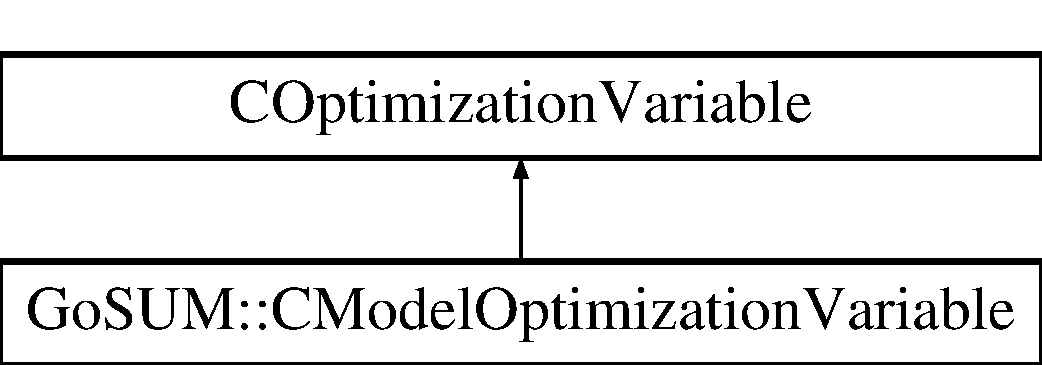
\includegraphics[height=2.000000cm]{class_c_optimization_variable}
\end{center}
\end{figure}
\subsection*{Public Member Functions}
\begin{DoxyCompactItemize}
\item 
\hyperlink{class_c_optimization_variable_a2af34948cc83069d6dd74a64397d85e0}{C\-Optimization\-Variable} ()
\item 
\hyperlink{class_c_optimization_variable_a349e830200ea6f76c47022e8aa6fd598}{C\-Optimization\-Variable} (double \-\_\-x\-L, double \-\_\-x\-U, double \-\_\-x0)
\item 
\hyperlink{class_c_optimization_variable_a410d3b78689566c940f3abd93bbfe0e4}{C\-Optimization\-Variable} (\hyperlink{class_c_optimization_variable}{C\-Optimization\-Variable} \&\-\_\-\-O)
\item 
virtual \hyperlink{class_c_optimization_variable_ab31271eb7663a4a48f4bed228bf54682}{$\sim$\-C\-Optimization\-Variable} ()
\item 
double \hyperlink{class_c_optimization_variable_af1b1ad75d642bf0455964e9357586bc2}{lower\-Bound} () const 
\begin{DoxyCompactList}\small\item\em Returns lower bound. \end{DoxyCompactList}\item 
double \hyperlink{class_c_optimization_variable_a9affc19ff1cfc507ab7e1df812d85bcb}{upper\-Bound} () const 
\begin{DoxyCompactList}\small\item\em Returns upper bound. \end{DoxyCompactList}\item 
double \hyperlink{class_c_optimization_variable_a2b61e79e0f74bb88afdcc788fabe1c6e}{initial\-Value} () const 
\begin{DoxyCompactList}\small\item\em Returns initial value. \end{DoxyCompactList}\item 
void \hyperlink{class_c_optimization_variable_ae92d781a0e9e38bc368ba69c996bb19a}{set\-Lower\-Bound} (double \-\_\-x\-L)
\begin{DoxyCompactList}\small\item\em Sets lower bound. \end{DoxyCompactList}\item 
void \hyperlink{class_c_optimization_variable_a6baed0144cd86d9032a2effa770a49f5}{set\-Upper\-Bound} (double \-\_\-x\-U)
\begin{DoxyCompactList}\small\item\em Sets upper bound. \end{DoxyCompactList}\item 
void \hyperlink{class_c_optimization_variable_a9b63133ea00f6aeed300c5ffd8ddabc8}{set\-Initial\-Value} (double \-\_\-x0)
\begin{DoxyCompactList}\small\item\em Sets inital value. \end{DoxyCompactList}\item 
void \hyperlink{class_c_optimization_variable_aaa2c98237b7a25ec3e111485fc631309}{set} (double \-\_\-x\-L, double \-\_\-x\-U, double \-\_\-x0)
\begin{DoxyCompactList}\small\item\em Sets lower bound, upper bound, initial value. \end{DoxyCompactList}\end{DoxyCompactItemize}
\subsection*{Protected Member Functions}
\begin{DoxyCompactItemize}
\item 
{\footnotesize template$<$class Archive $>$ }\\void \hyperlink{class_c_optimization_variable_ac7773d84cb5dcaf32b7f130fe60cbb8a}{serialize} (Archive \&ar, const unsigned int version)
\end{DoxyCompactItemize}
\subsection*{Protected Attributes}
\begin{DoxyCompactItemize}
\item 
double \hyperlink{class_c_optimization_variable_a64d40e05e5a9832e0e2aaebdbd105365}{x\-L}
\item 
double \hyperlink{class_c_optimization_variable_a549a16352636f3ec68729d197823716d}{x\-U}
\item 
double \hyperlink{class_c_optimization_variable_af67ef7c2faf37cb193309c7a540aee31}{x0}
\end{DoxyCompactItemize}
\subsection*{Friends}
\begin{DoxyCompactItemize}
\item 
class \hyperlink{class_c_optimization_variable_ac98d07dd8f7b70e16ccb9a01abf56b9c}{boost\-::serialization\-::access}
\begin{DoxyCompactList}\small\item\em Boost serialization. \end{DoxyCompactList}\end{DoxyCompactItemize}


\subsection{Constructor \& Destructor Documentation}
\hypertarget{class_c_optimization_variable_a2af34948cc83069d6dd74a64397d85e0}{\index{C\-Optimization\-Variable@{C\-Optimization\-Variable}!C\-Optimization\-Variable@{C\-Optimization\-Variable}}
\index{C\-Optimization\-Variable@{C\-Optimization\-Variable}!COptimizationVariable@{C\-Optimization\-Variable}}
\subsubsection[{C\-Optimization\-Variable}]{\setlength{\rightskip}{0pt plus 5cm}C\-Optimization\-Variable\-::\-C\-Optimization\-Variable (
\begin{DoxyParamCaption}
{}
\end{DoxyParamCaption}
)\hspace{0.3cm}{\ttfamily [inline]}}}\label{class_c_optimization_variable_a2af34948cc83069d6dd74a64397d85e0}
\hypertarget{class_c_optimization_variable_a349e830200ea6f76c47022e8aa6fd598}{\index{C\-Optimization\-Variable@{C\-Optimization\-Variable}!C\-Optimization\-Variable@{C\-Optimization\-Variable}}
\index{C\-Optimization\-Variable@{C\-Optimization\-Variable}!COptimizationVariable@{C\-Optimization\-Variable}}
\subsubsection[{C\-Optimization\-Variable}]{\setlength{\rightskip}{0pt plus 5cm}C\-Optimization\-Variable\-::\-C\-Optimization\-Variable (
\begin{DoxyParamCaption}
\item[{double}]{\-\_\-x\-L, }
\item[{double}]{\-\_\-x\-U, }
\item[{double}]{\-\_\-x0}
\end{DoxyParamCaption}
)\hspace{0.3cm}{\ttfamily [inline]}}}\label{class_c_optimization_variable_a349e830200ea6f76c47022e8aa6fd598}
\hypertarget{class_c_optimization_variable_a410d3b78689566c940f3abd93bbfe0e4}{\index{C\-Optimization\-Variable@{C\-Optimization\-Variable}!C\-Optimization\-Variable@{C\-Optimization\-Variable}}
\index{C\-Optimization\-Variable@{C\-Optimization\-Variable}!COptimizationVariable@{C\-Optimization\-Variable}}
\subsubsection[{C\-Optimization\-Variable}]{\setlength{\rightskip}{0pt plus 5cm}C\-Optimization\-Variable\-::\-C\-Optimization\-Variable (
\begin{DoxyParamCaption}
\item[{{\bf C\-Optimization\-Variable} \&}]{\-\_\-\-O}
\end{DoxyParamCaption}
)\hspace{0.3cm}{\ttfamily [inline]}}}\label{class_c_optimization_variable_a410d3b78689566c940f3abd93bbfe0e4}
\hypertarget{class_c_optimization_variable_ab31271eb7663a4a48f4bed228bf54682}{\index{C\-Optimization\-Variable@{C\-Optimization\-Variable}!$\sim$\-C\-Optimization\-Variable@{$\sim$\-C\-Optimization\-Variable}}
\index{$\sim$\-C\-Optimization\-Variable@{$\sim$\-C\-Optimization\-Variable}!COptimizationVariable@{C\-Optimization\-Variable}}
\subsubsection[{$\sim$\-C\-Optimization\-Variable}]{\setlength{\rightskip}{0pt plus 5cm}virtual C\-Optimization\-Variable\-::$\sim$\-C\-Optimization\-Variable (
\begin{DoxyParamCaption}
{}
\end{DoxyParamCaption}
)\hspace{0.3cm}{\ttfamily [inline]}, {\ttfamily [virtual]}}}\label{class_c_optimization_variable_ab31271eb7663a4a48f4bed228bf54682}


\subsection{Member Function Documentation}
\hypertarget{class_c_optimization_variable_a2b61e79e0f74bb88afdcc788fabe1c6e}{\index{C\-Optimization\-Variable@{C\-Optimization\-Variable}!initial\-Value@{initial\-Value}}
\index{initial\-Value@{initial\-Value}!COptimizationVariable@{C\-Optimization\-Variable}}
\subsubsection[{initial\-Value}]{\setlength{\rightskip}{0pt plus 5cm}double C\-Optimization\-Variable\-::initial\-Value (
\begin{DoxyParamCaption}
{}
\end{DoxyParamCaption}
) const\hspace{0.3cm}{\ttfamily [inline]}}}\label{class_c_optimization_variable_a2b61e79e0f74bb88afdcc788fabe1c6e}


Returns initial value. 

\hypertarget{class_c_optimization_variable_af1b1ad75d642bf0455964e9357586bc2}{\index{C\-Optimization\-Variable@{C\-Optimization\-Variable}!lower\-Bound@{lower\-Bound}}
\index{lower\-Bound@{lower\-Bound}!COptimizationVariable@{C\-Optimization\-Variable}}
\subsubsection[{lower\-Bound}]{\setlength{\rightskip}{0pt plus 5cm}double C\-Optimization\-Variable\-::lower\-Bound (
\begin{DoxyParamCaption}
{}
\end{DoxyParamCaption}
) const\hspace{0.3cm}{\ttfamily [inline]}}}\label{class_c_optimization_variable_af1b1ad75d642bf0455964e9357586bc2}


Returns lower bound. 

\hypertarget{class_c_optimization_variable_ac7773d84cb5dcaf32b7f130fe60cbb8a}{\index{C\-Optimization\-Variable@{C\-Optimization\-Variable}!serialize@{serialize}}
\index{serialize@{serialize}!COptimizationVariable@{C\-Optimization\-Variable}}
\subsubsection[{serialize}]{\setlength{\rightskip}{0pt plus 5cm}template$<$class Archive $>$ void C\-Optimization\-Variable\-::serialize (
\begin{DoxyParamCaption}
\item[{Archive \&}]{ar, }
\item[{const unsigned int}]{version}
\end{DoxyParamCaption}
)\hspace{0.3cm}{\ttfamily [inline]}, {\ttfamily [protected]}}}\label{class_c_optimization_variable_ac7773d84cb5dcaf32b7f130fe60cbb8a}


Reimplemented in \hyperlink{class_go_s_u_m_1_1_c_model_optimization_variable_ac2e916e3523fec4487a8f567bb0a1af9}{Go\-S\-U\-M\-::\-C\-Model\-Optimization\-Variable}.

\hypertarget{class_c_optimization_variable_aaa2c98237b7a25ec3e111485fc631309}{\index{C\-Optimization\-Variable@{C\-Optimization\-Variable}!set@{set}}
\index{set@{set}!COptimizationVariable@{C\-Optimization\-Variable}}
\subsubsection[{set}]{\setlength{\rightskip}{0pt plus 5cm}void C\-Optimization\-Variable\-::set (
\begin{DoxyParamCaption}
\item[{double}]{\-\_\-x\-L, }
\item[{double}]{\-\_\-x\-U, }
\item[{double}]{\-\_\-x0}
\end{DoxyParamCaption}
)}}\label{class_c_optimization_variable_aaa2c98237b7a25ec3e111485fc631309}


Sets lower bound, upper bound, initial value. 

\hypertarget{class_c_optimization_variable_a9b63133ea00f6aeed300c5ffd8ddabc8}{\index{C\-Optimization\-Variable@{C\-Optimization\-Variable}!set\-Initial\-Value@{set\-Initial\-Value}}
\index{set\-Initial\-Value@{set\-Initial\-Value}!COptimizationVariable@{C\-Optimization\-Variable}}
\subsubsection[{set\-Initial\-Value}]{\setlength{\rightskip}{0pt plus 5cm}void C\-Optimization\-Variable\-::set\-Initial\-Value (
\begin{DoxyParamCaption}
\item[{double}]{\-\_\-x0}
\end{DoxyParamCaption}
)}}\label{class_c_optimization_variable_a9b63133ea00f6aeed300c5ffd8ddabc8}


Sets inital value. 

\hypertarget{class_c_optimization_variable_ae92d781a0e9e38bc368ba69c996bb19a}{\index{C\-Optimization\-Variable@{C\-Optimization\-Variable}!set\-Lower\-Bound@{set\-Lower\-Bound}}
\index{set\-Lower\-Bound@{set\-Lower\-Bound}!COptimizationVariable@{C\-Optimization\-Variable}}
\subsubsection[{set\-Lower\-Bound}]{\setlength{\rightskip}{0pt plus 5cm}void C\-Optimization\-Variable\-::set\-Lower\-Bound (
\begin{DoxyParamCaption}
\item[{double}]{\-\_\-x\-L}
\end{DoxyParamCaption}
)}}\label{class_c_optimization_variable_ae92d781a0e9e38bc368ba69c996bb19a}


Sets lower bound. 

\hypertarget{class_c_optimization_variable_a6baed0144cd86d9032a2effa770a49f5}{\index{C\-Optimization\-Variable@{C\-Optimization\-Variable}!set\-Upper\-Bound@{set\-Upper\-Bound}}
\index{set\-Upper\-Bound@{set\-Upper\-Bound}!COptimizationVariable@{C\-Optimization\-Variable}}
\subsubsection[{set\-Upper\-Bound}]{\setlength{\rightskip}{0pt plus 5cm}void C\-Optimization\-Variable\-::set\-Upper\-Bound (
\begin{DoxyParamCaption}
\item[{double}]{\-\_\-x\-U}
\end{DoxyParamCaption}
)}}\label{class_c_optimization_variable_a6baed0144cd86d9032a2effa770a49f5}


Sets upper bound. 

\hypertarget{class_c_optimization_variable_a9affc19ff1cfc507ab7e1df812d85bcb}{\index{C\-Optimization\-Variable@{C\-Optimization\-Variable}!upper\-Bound@{upper\-Bound}}
\index{upper\-Bound@{upper\-Bound}!COptimizationVariable@{C\-Optimization\-Variable}}
\subsubsection[{upper\-Bound}]{\setlength{\rightskip}{0pt plus 5cm}double C\-Optimization\-Variable\-::upper\-Bound (
\begin{DoxyParamCaption}
{}
\end{DoxyParamCaption}
) const\hspace{0.3cm}{\ttfamily [inline]}}}\label{class_c_optimization_variable_a9affc19ff1cfc507ab7e1df812d85bcb}


Returns upper bound. 



\subsection{Friends And Related Function Documentation}
\hypertarget{class_c_optimization_variable_ac98d07dd8f7b70e16ccb9a01abf56b9c}{\index{C\-Optimization\-Variable@{C\-Optimization\-Variable}!boost\-::serialization\-::access@{boost\-::serialization\-::access}}
\index{boost\-::serialization\-::access@{boost\-::serialization\-::access}!COptimizationVariable@{C\-Optimization\-Variable}}
\subsubsection[{boost\-::serialization\-::access}]{\setlength{\rightskip}{0pt plus 5cm}friend class boost\-::serialization\-::access\hspace{0.3cm}{\ttfamily [friend]}}}\label{class_c_optimization_variable_ac98d07dd8f7b70e16ccb9a01abf56b9c}


Boost serialization. 



\subsection{Member Data Documentation}
\hypertarget{class_c_optimization_variable_af67ef7c2faf37cb193309c7a540aee31}{\index{C\-Optimization\-Variable@{C\-Optimization\-Variable}!x0@{x0}}
\index{x0@{x0}!COptimizationVariable@{C\-Optimization\-Variable}}
\subsubsection[{x0}]{\setlength{\rightskip}{0pt plus 5cm}double C\-Optimization\-Variable\-::x0\hspace{0.3cm}{\ttfamily [protected]}}}\label{class_c_optimization_variable_af67ef7c2faf37cb193309c7a540aee31}
Holds lower bound, upper bound and initial value of a optimization variable. \hypertarget{class_c_optimization_variable_a64d40e05e5a9832e0e2aaebdbd105365}{\index{C\-Optimization\-Variable@{C\-Optimization\-Variable}!x\-L@{x\-L}}
\index{x\-L@{x\-L}!COptimizationVariable@{C\-Optimization\-Variable}}
\subsubsection[{x\-L}]{\setlength{\rightskip}{0pt plus 5cm}double C\-Optimization\-Variable\-::x\-L\hspace{0.3cm}{\ttfamily [protected]}}}\label{class_c_optimization_variable_a64d40e05e5a9832e0e2aaebdbd105365}
\hypertarget{class_c_optimization_variable_a549a16352636f3ec68729d197823716d}{\index{C\-Optimization\-Variable@{C\-Optimization\-Variable}!x\-U@{x\-U}}
\index{x\-U@{x\-U}!COptimizationVariable@{C\-Optimization\-Variable}}
\subsubsection[{x\-U}]{\setlength{\rightskip}{0pt plus 5cm}double C\-Optimization\-Variable\-::x\-U\hspace{0.3cm}{\ttfamily [protected]}}}\label{class_c_optimization_variable_a549a16352636f3ec68729d197823716d}


The documentation for this class was generated from the following files\-:\begin{DoxyCompactItemize}
\item 
C\-:/\-Development/core/\hyperlink{_optimization_problem_8h}{Optimization\-Problem.\-h}\item 
C\-:/\-Development/core/\hyperlink{_optimization_problem_8cpp}{Optimization\-Problem.\-cpp}\end{DoxyCompactItemize}

\hypertarget{class_go_s_u_m_1_1_c_original_optimization_problem}{\section{Go\-S\-U\-M\-:\-:C\-Original\-Optimization\-Problem Class Reference}
\label{class_go_s_u_m_1_1_c_original_optimization_problem}\index{Go\-S\-U\-M\-::\-C\-Original\-Optimization\-Problem@{Go\-S\-U\-M\-::\-C\-Original\-Optimization\-Problem}}
}


Class for the optimization problem based on \hyperlink{struct_go_s_u_m}{Go\-S\-U\-M} analyitical model.  




{\ttfamily \#include $<$Parser\-Optimization\-Problem.\-h$>$}

Inheritance diagram for Go\-S\-U\-M\-:\-:C\-Original\-Optimization\-Problem\-:\begin{figure}[H]
\begin{center}
\leavevmode
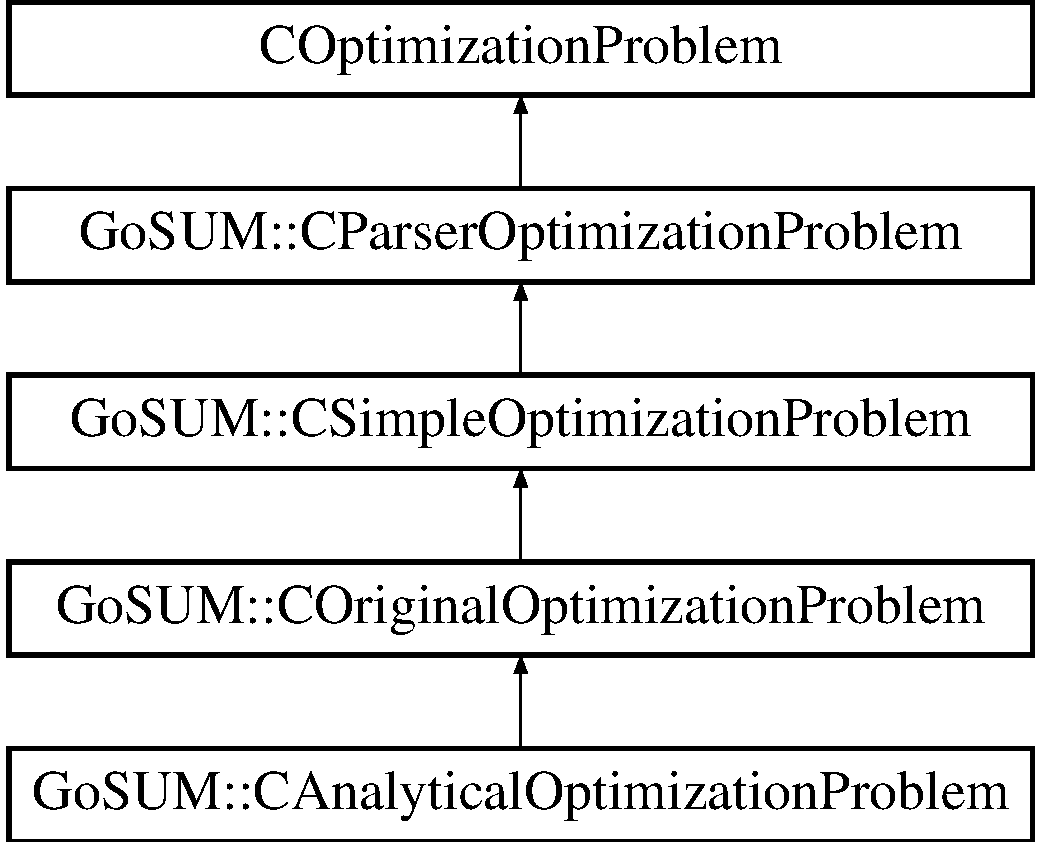
\includegraphics[height=5.000000cm]{class_go_s_u_m_1_1_c_original_optimization_problem}
\end{center}
\end{figure}
\subsection*{Public Member Functions}
\begin{DoxyCompactItemize}
\item 
\hyperlink{class_go_s_u_m_1_1_c_original_optimization_problem_a3a7ca7ef6350e169b49d23a1f170413e}{C\-Original\-Optimization\-Problem} (\hyperlink{class_go_s_u_m_1_1_c_input_parameters}{C\-Input\-Parameters} $\ast$\-\_\-p\-I\-P, \hyperlink{class_go_s_u_m_1_1_c_output_states}{C\-Output\-States} $\ast$\-\_\-p\-O\-S)
\item 
virtual \hyperlink{class_go_s_u_m_1_1_c_original_optimization_problem_afd4e36fcf4757eccdcf0ce5d35a9f070}{$\sim$\-C\-Original\-Optimization\-Problem} ()
\item 
virtual void \hyperlink{class_go_s_u_m_1_1_c_original_optimization_problem_aa2473c8014cf051d66ecbe6107043b6a}{open\-Optimization} ()
\item 
virtual void \hyperlink{class_go_s_u_m_1_1_c_original_optimization_problem_a75b28528cda5b1be7bdc2cc4a309a314}{close\-Optimization} ()
\begin{DoxyCompactList}\small\item\em Opens, i.\-e. prepares optimization. \end{DoxyCompactList}\item 
Array\-Xd \hyperlink{class_go_s_u_m_1_1_c_original_optimization_problem_a3ad565122964e4fdec8156f6457c582e}{input\-Point2\-Model\-Point} (const Array\-Xd \&\-\_\-ip)
\begin{DoxyCompactList}\small\item\em Closes optimization, i.\-e. closes what was opened in open\-Optimization. \end{DoxyCompactList}\end{DoxyCompactItemize}
\subsection*{Protected Member Functions}
\begin{DoxyCompactItemize}
\item 
{\footnotesize template$<$class Archive $>$ }\\void \hyperlink{class_go_s_u_m_1_1_c_original_optimization_problem_a41f4a21189b39fcdb0d820d2f8348475}{serialize} (Archive \&ar, const unsigned int version)
\item 
\hyperlink{class_go_s_u_m_1_1_c_original_optimization_problem_a6df1f069274ee592d945be3427e0e49a}{C\-Original\-Optimization\-Problem} ()
\item 
virtual void \hyperlink{class_go_s_u_m_1_1_c_original_optimization_problem_aabc85a11abb23fdfe5b99f8d141ae4bb}{set\-Variable\-Names} ()
\begin{DoxyCompactList}\small\item\em Sets variable names for the parser. \end{DoxyCompactList}\end{DoxyCompactItemize}
\subsection*{Protected Attributes}
\begin{DoxyCompactItemize}
\item 
\hyperlink{class_go_s_u_m_1_1_c_output_states}{C\-Output\-States} $\ast$ \hyperlink{class_go_s_u_m_1_1_c_original_optimization_problem_a7c3c4d727506f3c503768d70c7fd0f73}{p\-O\-S}
\end{DoxyCompactItemize}
\subsection*{Friends}
\begin{DoxyCompactItemize}
\item 
class \hyperlink{class_go_s_u_m_1_1_c_original_optimization_problem_ac98d07dd8f7b70e16ccb9a01abf56b9c}{boost\-::serialization\-::access}
\begin{DoxyCompactList}\small\item\em Boost serialization. \end{DoxyCompactList}\end{DoxyCompactItemize}
\subsection*{Additional Inherited Members}


\subsection{Detailed Description}
Class for the optimization problem based on \hyperlink{struct_go_s_u_m}{Go\-S\-U\-M} analyitical model. 

\subsection{Constructor \& Destructor Documentation}
\hypertarget{class_go_s_u_m_1_1_c_original_optimization_problem_a6df1f069274ee592d945be3427e0e49a}{\index{Go\-S\-U\-M\-::\-C\-Original\-Optimization\-Problem@{Go\-S\-U\-M\-::\-C\-Original\-Optimization\-Problem}!C\-Original\-Optimization\-Problem@{C\-Original\-Optimization\-Problem}}
\index{C\-Original\-Optimization\-Problem@{C\-Original\-Optimization\-Problem}!GoSUM::COriginalOptimizationProblem@{Go\-S\-U\-M\-::\-C\-Original\-Optimization\-Problem}}
\subsubsection[{C\-Original\-Optimization\-Problem}]{\setlength{\rightskip}{0pt plus 5cm}Go\-S\-U\-M\-::\-C\-Original\-Optimization\-Problem\-::\-C\-Original\-Optimization\-Problem (
\begin{DoxyParamCaption}
{}
\end{DoxyParamCaption}
)\hspace{0.3cm}{\ttfamily [inline]}, {\ttfamily [protected]}}}\label{class_go_s_u_m_1_1_c_original_optimization_problem_a6df1f069274ee592d945be3427e0e49a}
\hypertarget{class_go_s_u_m_1_1_c_original_optimization_problem_a3a7ca7ef6350e169b49d23a1f170413e}{\index{Go\-S\-U\-M\-::\-C\-Original\-Optimization\-Problem@{Go\-S\-U\-M\-::\-C\-Original\-Optimization\-Problem}!C\-Original\-Optimization\-Problem@{C\-Original\-Optimization\-Problem}}
\index{C\-Original\-Optimization\-Problem@{C\-Original\-Optimization\-Problem}!GoSUM::COriginalOptimizationProblem@{Go\-S\-U\-M\-::\-C\-Original\-Optimization\-Problem}}
\subsubsection[{C\-Original\-Optimization\-Problem}]{\setlength{\rightskip}{0pt plus 5cm}Go\-S\-U\-M\-::\-C\-Original\-Optimization\-Problem\-::\-C\-Original\-Optimization\-Problem (
\begin{DoxyParamCaption}
\item[{{\bf C\-Input\-Parameters} $\ast$}]{\-\_\-p\-I\-P, }
\item[{{\bf C\-Output\-States} $\ast$}]{\-\_\-p\-O\-S}
\end{DoxyParamCaption}
)\hspace{0.3cm}{\ttfamily [inline]}}}\label{class_go_s_u_m_1_1_c_original_optimization_problem_a3a7ca7ef6350e169b49d23a1f170413e}
\hypertarget{class_go_s_u_m_1_1_c_original_optimization_problem_afd4e36fcf4757eccdcf0ce5d35a9f070}{\index{Go\-S\-U\-M\-::\-C\-Original\-Optimization\-Problem@{Go\-S\-U\-M\-::\-C\-Original\-Optimization\-Problem}!$\sim$\-C\-Original\-Optimization\-Problem@{$\sim$\-C\-Original\-Optimization\-Problem}}
\index{$\sim$\-C\-Original\-Optimization\-Problem@{$\sim$\-C\-Original\-Optimization\-Problem}!GoSUM::COriginalOptimizationProblem@{Go\-S\-U\-M\-::\-C\-Original\-Optimization\-Problem}}
\subsubsection[{$\sim$\-C\-Original\-Optimization\-Problem}]{\setlength{\rightskip}{0pt plus 5cm}virtual Go\-S\-U\-M\-::\-C\-Original\-Optimization\-Problem\-::$\sim$\-C\-Original\-Optimization\-Problem (
\begin{DoxyParamCaption}
{}
\end{DoxyParamCaption}
)\hspace{0.3cm}{\ttfamily [inline]}, {\ttfamily [virtual]}}}\label{class_go_s_u_m_1_1_c_original_optimization_problem_afd4e36fcf4757eccdcf0ce5d35a9f070}


\subsection{Member Function Documentation}
\hypertarget{class_go_s_u_m_1_1_c_original_optimization_problem_a75b28528cda5b1be7bdc2cc4a309a314}{\index{Go\-S\-U\-M\-::\-C\-Original\-Optimization\-Problem@{Go\-S\-U\-M\-::\-C\-Original\-Optimization\-Problem}!close\-Optimization@{close\-Optimization}}
\index{close\-Optimization@{close\-Optimization}!GoSUM::COriginalOptimizationProblem@{Go\-S\-U\-M\-::\-C\-Original\-Optimization\-Problem}}
\subsubsection[{close\-Optimization}]{\setlength{\rightskip}{0pt plus 5cm}virtual void Go\-S\-U\-M\-::\-C\-Original\-Optimization\-Problem\-::close\-Optimization (
\begin{DoxyParamCaption}
{}
\end{DoxyParamCaption}
)\hspace{0.3cm}{\ttfamily [inline]}, {\ttfamily [virtual]}}}\label{class_go_s_u_m_1_1_c_original_optimization_problem_a75b28528cda5b1be7bdc2cc4a309a314}


Opens, i.\-e. prepares optimization. 



Reimplemented from \hyperlink{class_go_s_u_m_1_1_c_simple_optimization_problem_af34b88f099f94727611b79d5f5ca4e9a}{Go\-S\-U\-M\-::\-C\-Simple\-Optimization\-Problem}.

\hypertarget{class_go_s_u_m_1_1_c_original_optimization_problem_a3ad565122964e4fdec8156f6457c582e}{\index{Go\-S\-U\-M\-::\-C\-Original\-Optimization\-Problem@{Go\-S\-U\-M\-::\-C\-Original\-Optimization\-Problem}!input\-Point2\-Model\-Point@{input\-Point2\-Model\-Point}}
\index{input\-Point2\-Model\-Point@{input\-Point2\-Model\-Point}!GoSUM::COriginalOptimizationProblem@{Go\-S\-U\-M\-::\-C\-Original\-Optimization\-Problem}}
\subsubsection[{input\-Point2\-Model\-Point}]{\setlength{\rightskip}{0pt plus 5cm}Array\-Xd Go\-S\-U\-M\-::\-C\-Original\-Optimization\-Problem\-::input\-Point2\-Model\-Point (
\begin{DoxyParamCaption}
\item[{const Array\-Xd \&}]{\-\_\-ip}
\end{DoxyParamCaption}
)}}\label{class_go_s_u_m_1_1_c_original_optimization_problem_a3ad565122964e4fdec8156f6457c582e}


Closes optimization, i.\-e. closes what was opened in open\-Optimization. 

Converts input parameter point to model point. 

Reimplemented from \hyperlink{class_go_s_u_m_1_1_c_simple_optimization_problem_a1eb9802fcaf98b032e0ad2f5c70541ce}{Go\-S\-U\-M\-::\-C\-Simple\-Optimization\-Problem}.



Reimplemented in \hyperlink{class_go_s_u_m_1_1_c_analytical_optimization_problem_a83cf54606759ec8e5cb20cbb0b0ce6f5}{Go\-S\-U\-M\-::\-C\-Analytical\-Optimization\-Problem}.

\hypertarget{class_go_s_u_m_1_1_c_original_optimization_problem_aa2473c8014cf051d66ecbe6107043b6a}{\index{Go\-S\-U\-M\-::\-C\-Original\-Optimization\-Problem@{Go\-S\-U\-M\-::\-C\-Original\-Optimization\-Problem}!open\-Optimization@{open\-Optimization}}
\index{open\-Optimization@{open\-Optimization}!GoSUM::COriginalOptimizationProblem@{Go\-S\-U\-M\-::\-C\-Original\-Optimization\-Problem}}
\subsubsection[{open\-Optimization}]{\setlength{\rightskip}{0pt plus 5cm}virtual void Go\-S\-U\-M\-::\-C\-Original\-Optimization\-Problem\-::open\-Optimization (
\begin{DoxyParamCaption}
{}
\end{DoxyParamCaption}
)\hspace{0.3cm}{\ttfamily [inline]}, {\ttfamily [virtual]}}}\label{class_go_s_u_m_1_1_c_original_optimization_problem_aa2473c8014cf051d66ecbe6107043b6a}


Reimplemented from \hyperlink{class_go_s_u_m_1_1_c_simple_optimization_problem_a772db1ec2c35c78a4b68551969e4083c}{Go\-S\-U\-M\-::\-C\-Simple\-Optimization\-Problem}.

\hypertarget{class_go_s_u_m_1_1_c_original_optimization_problem_a41f4a21189b39fcdb0d820d2f8348475}{\index{Go\-S\-U\-M\-::\-C\-Original\-Optimization\-Problem@{Go\-S\-U\-M\-::\-C\-Original\-Optimization\-Problem}!serialize@{serialize}}
\index{serialize@{serialize}!GoSUM::COriginalOptimizationProblem@{Go\-S\-U\-M\-::\-C\-Original\-Optimization\-Problem}}
\subsubsection[{serialize}]{\setlength{\rightskip}{0pt plus 5cm}template$<$class Archive $>$ void Go\-S\-U\-M\-::\-C\-Original\-Optimization\-Problem\-::serialize (
\begin{DoxyParamCaption}
\item[{Archive \&}]{ar, }
\item[{const unsigned int}]{version}
\end{DoxyParamCaption}
)\hspace{0.3cm}{\ttfamily [protected]}}}\label{class_go_s_u_m_1_1_c_original_optimization_problem_a41f4a21189b39fcdb0d820d2f8348475}


Reimplemented from \hyperlink{class_go_s_u_m_1_1_c_simple_optimization_problem_a627c6cfdc256739e723cbdbf1a61c007}{Go\-S\-U\-M\-::\-C\-Simple\-Optimization\-Problem}.



Reimplemented in \hyperlink{class_go_s_u_m_1_1_c_analytical_optimization_problem_a258b0f6d24b501a1bb5ca1e65a06e8c5}{Go\-S\-U\-M\-::\-C\-Analytical\-Optimization\-Problem}.

\hypertarget{class_go_s_u_m_1_1_c_original_optimization_problem_aabc85a11abb23fdfe5b99f8d141ae4bb}{\index{Go\-S\-U\-M\-::\-C\-Original\-Optimization\-Problem@{Go\-S\-U\-M\-::\-C\-Original\-Optimization\-Problem}!set\-Variable\-Names@{set\-Variable\-Names}}
\index{set\-Variable\-Names@{set\-Variable\-Names}!GoSUM::COriginalOptimizationProblem@{Go\-S\-U\-M\-::\-C\-Original\-Optimization\-Problem}}
\subsubsection[{set\-Variable\-Names}]{\setlength{\rightskip}{0pt plus 5cm}void Go\-S\-U\-M\-::\-C\-Original\-Optimization\-Problem\-::set\-Variable\-Names (
\begin{DoxyParamCaption}
{}
\end{DoxyParamCaption}
)\hspace{0.3cm}{\ttfamily [protected]}, {\ttfamily [virtual]}}}\label{class_go_s_u_m_1_1_c_original_optimization_problem_aabc85a11abb23fdfe5b99f8d141ae4bb}


Sets variable names for the parser. 



Reimplemented from \hyperlink{class_go_s_u_m_1_1_c_simple_optimization_problem_a051a218199a044cd97ba46a1cf9175f7}{Go\-S\-U\-M\-::\-C\-Simple\-Optimization\-Problem}.



\subsection{Friends And Related Function Documentation}
\hypertarget{class_go_s_u_m_1_1_c_original_optimization_problem_ac98d07dd8f7b70e16ccb9a01abf56b9c}{\index{Go\-S\-U\-M\-::\-C\-Original\-Optimization\-Problem@{Go\-S\-U\-M\-::\-C\-Original\-Optimization\-Problem}!boost\-::serialization\-::access@{boost\-::serialization\-::access}}
\index{boost\-::serialization\-::access@{boost\-::serialization\-::access}!GoSUM::COriginalOptimizationProblem@{Go\-S\-U\-M\-::\-C\-Original\-Optimization\-Problem}}
\subsubsection[{boost\-::serialization\-::access}]{\setlength{\rightskip}{0pt plus 5cm}friend class boost\-::serialization\-::access\hspace{0.3cm}{\ttfamily [friend]}}}\label{class_go_s_u_m_1_1_c_original_optimization_problem_ac98d07dd8f7b70e16ccb9a01abf56b9c}


Boost serialization. 



\subsection{Member Data Documentation}
\hypertarget{class_go_s_u_m_1_1_c_original_optimization_problem_a7c3c4d727506f3c503768d70c7fd0f73}{\index{Go\-S\-U\-M\-::\-C\-Original\-Optimization\-Problem@{Go\-S\-U\-M\-::\-C\-Original\-Optimization\-Problem}!p\-O\-S@{p\-O\-S}}
\index{p\-O\-S@{p\-O\-S}!GoSUM::COriginalOptimizationProblem@{Go\-S\-U\-M\-::\-C\-Original\-Optimization\-Problem}}
\subsubsection[{p\-O\-S}]{\setlength{\rightskip}{0pt plus 5cm}{\bf C\-Output\-States}$\ast$ Go\-S\-U\-M\-::\-C\-Original\-Optimization\-Problem\-::p\-O\-S\hspace{0.3cm}{\ttfamily [protected]}}}\label{class_go_s_u_m_1_1_c_original_optimization_problem_a7c3c4d727506f3c503768d70c7fd0f73}
Points to output states. 

The documentation for this class was generated from the following files\-:\begin{DoxyCompactItemize}
\item 
C\-:/\-Development/core/\hyperlink{_parser_optimization_problem_8h}{Parser\-Optimization\-Problem.\-h}\item 
C\-:/\-Development/core/\hyperlink{_parser_optimization_problem_8cpp}{Parser\-Optimization\-Problem.\-cpp}\end{DoxyCompactItemize}

\hypertarget{class_go_s_u_m_1_1_c_output_states}{\section{Go\-S\-U\-M\-:\-:C\-Output\-States Class Reference}
\label{class_go_s_u_m_1_1_c_output_states}\index{Go\-S\-U\-M\-::\-C\-Output\-States@{Go\-S\-U\-M\-::\-C\-Output\-States}}
}


Class for \hyperlink{struct_go_s_u_m}{Go\-S\-U\-M} output states.  




{\ttfamily \#include $<$Model.\-h$>$}

Inheritance diagram for Go\-S\-U\-M\-:\-:C\-Output\-States\-:\begin{figure}[H]
\begin{center}
\leavevmode
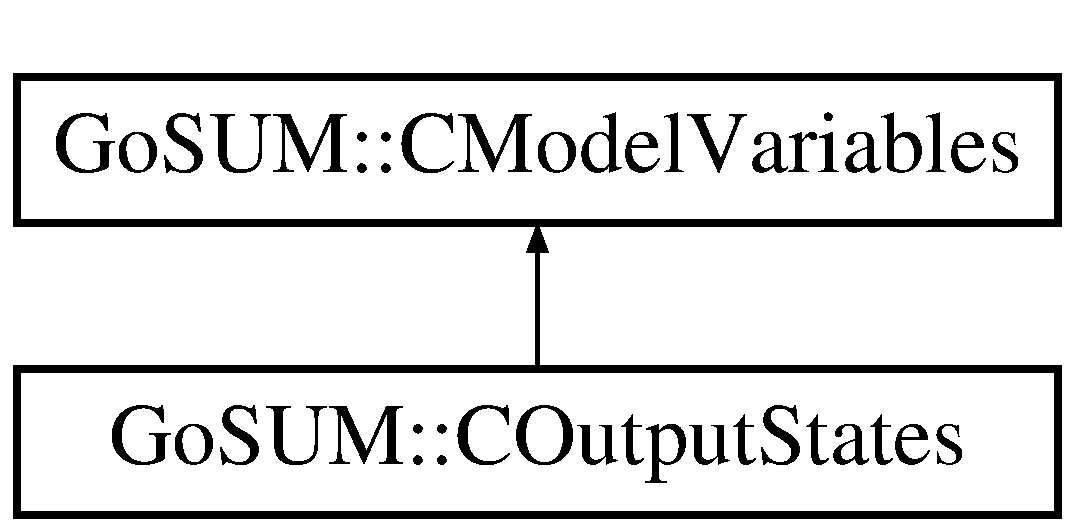
\includegraphics[height=2.000000cm]{class_go_s_u_m_1_1_c_output_states}
\end{center}
\end{figure}
\subsection*{Public Member Functions}
\begin{DoxyCompactItemize}
\item 
\hyperlink{class_go_s_u_m_1_1_c_output_states_a78ee554531ace49e677ac5f6aabb1793}{C\-Output\-States} ()
\item 
virtual \hyperlink{class_go_s_u_m_1_1_c_output_states_a7243b706e954618d47c90d69a28f5ecc}{$\sim$\-C\-Output\-States} ()
\item 
bool \hyperlink{class_go_s_u_m_1_1_c_output_states_ac90deb06c63df80bc34ee2c664562a43}{set\-Evaluator\-Compatible} (const \hyperlink{class_go_s_u_m_1_1_c_input_parameters}{C\-Input\-Parameters} \&inputs)
\item 
void \hyperlink{class_go_s_u_m_1_1_c_output_states_a8041e00b80f9027b5f949c6dd1dcee74}{evaluate} (const \hyperlink{class_go_s_u_m_1_1_c_input_parameters}{C\-Input\-Parameters} \&inputs)
\begin{DoxyCompactList}\small\item\em Starts end joins multiple threads for model function evaluation. \end{DoxyCompactList}\item 
void \hyperlink{class_go_s_u_m_1_1_c_output_states_ad286b10860c762d05821da1f81c8b4de}{open\-Evaluation} (const \hyperlink{class_go_s_u_m_1_1_c_input_parameters}{C\-Input\-Parameters} \&inputs)
\item 
Array\-Xd \hyperlink{class_go_s_u_m_1_1_c_output_states_a7ba935ed20daaee5deabf1d99dbecc6e}{evaluate} (const Array\-Xd \&X)
\begin{DoxyCompactList}\small\item\em Opens evaluation on single input parameter n-\/tuples. \end{DoxyCompactList}\item 
void \hyperlink{class_go_s_u_m_1_1_c_output_states_a281641905b4c5bcaa6b0beb1a5c880dc}{close\-Evaluation} ()
\item 
void \hyperlink{class_go_s_u_m_1_1_c_output_states_ac8f7c955c7e0b1257bb6323f9b23f565}{set\-Progress\-Slot} (boost\-::function$<$ void()$>$ \-\_\-progress\-Slot)
\begin{DoxyCompactList}\small\item\em Sets external progress slot. \end{DoxyCompactList}\end{DoxyCompactItemize}
\subsection*{Public Attributes}
\begin{DoxyCompactItemize}
\item 
boost\-::function$<$ void()$>$ \hyperlink{class_go_s_u_m_1_1_c_output_states_af87022e02d37a1ed2c804776f15b30b7}{progress\-Slot}
\begin{DoxyCompactList}\small\item\em Closes evaluation on single input parameter n-\/tuples. \end{DoxyCompactList}\end{DoxyCompactItemize}
\subsection*{Private Member Functions}
\begin{DoxyCompactItemize}
\item 
{\footnotesize template$<$class Archive $>$ }\\void \hyperlink{class_go_s_u_m_1_1_c_output_states_a02da6bf9a4d7d11010670ab6525d7ac4}{serialize} (Archive \&ar, const unsigned int version)
\end{DoxyCompactItemize}
\subsection*{Private Attributes}
\begin{DoxyCompactItemize}
\item 
\hyperlink{class_go_s_u_m_1_1_c_model_evaluator}{Go\-S\-U\-M\-::\-C\-Model\-Evaluator} $\ast$ \hyperlink{class_go_s_u_m_1_1_c_output_states_ace5684dae11c9a0d432daddd623d8b62}{p\-E}
\end{DoxyCompactItemize}
\subsection*{Friends}
\begin{DoxyCompactItemize}
\item 
class \hyperlink{class_go_s_u_m_1_1_c_output_states_ac98d07dd8f7b70e16ccb9a01abf56b9c}{boost\-::serialization\-::access}
\begin{DoxyCompactList}\small\item\em boost serialization \end{DoxyCompactList}\end{DoxyCompactItemize}
\subsection*{Additional Inherited Members}


\subsection{Detailed Description}
Class for \hyperlink{struct_go_s_u_m}{Go\-S\-U\-M} output states. 

\subsection{Constructor \& Destructor Documentation}
\hypertarget{class_go_s_u_m_1_1_c_output_states_a78ee554531ace49e677ac5f6aabb1793}{\index{Go\-S\-U\-M\-::\-C\-Output\-States@{Go\-S\-U\-M\-::\-C\-Output\-States}!C\-Output\-States@{C\-Output\-States}}
\index{C\-Output\-States@{C\-Output\-States}!GoSUM::COutputStates@{Go\-S\-U\-M\-::\-C\-Output\-States}}
\subsubsection[{C\-Output\-States}]{\setlength{\rightskip}{0pt plus 5cm}Go\-S\-U\-M\-::\-C\-Output\-States\-::\-C\-Output\-States (
\begin{DoxyParamCaption}
{}
\end{DoxyParamCaption}
)\hspace{0.3cm}{\ttfamily [inline]}}}\label{class_go_s_u_m_1_1_c_output_states_a78ee554531ace49e677ac5f6aabb1793}
\hypertarget{class_go_s_u_m_1_1_c_output_states_a7243b706e954618d47c90d69a28f5ecc}{\index{Go\-S\-U\-M\-::\-C\-Output\-States@{Go\-S\-U\-M\-::\-C\-Output\-States}!$\sim$\-C\-Output\-States@{$\sim$\-C\-Output\-States}}
\index{$\sim$\-C\-Output\-States@{$\sim$\-C\-Output\-States}!GoSUM::COutputStates@{Go\-S\-U\-M\-::\-C\-Output\-States}}
\subsubsection[{$\sim$\-C\-Output\-States}]{\setlength{\rightskip}{0pt plus 5cm}virtual Go\-S\-U\-M\-::\-C\-Output\-States\-::$\sim$\-C\-Output\-States (
\begin{DoxyParamCaption}
{}
\end{DoxyParamCaption}
)\hspace{0.3cm}{\ttfamily [inline]}, {\ttfamily [virtual]}}}\label{class_go_s_u_m_1_1_c_output_states_a7243b706e954618d47c90d69a28f5ecc}


\subsection{Member Function Documentation}
\hypertarget{class_go_s_u_m_1_1_c_output_states_a281641905b4c5bcaa6b0beb1a5c880dc}{\index{Go\-S\-U\-M\-::\-C\-Output\-States@{Go\-S\-U\-M\-::\-C\-Output\-States}!close\-Evaluation@{close\-Evaluation}}
\index{close\-Evaluation@{close\-Evaluation}!GoSUM::COutputStates@{Go\-S\-U\-M\-::\-C\-Output\-States}}
\subsubsection[{close\-Evaluation}]{\setlength{\rightskip}{0pt plus 5cm}void Go\-S\-U\-M\-::\-C\-Output\-States\-::close\-Evaluation (
\begin{DoxyParamCaption}
{}
\end{DoxyParamCaption}
)}}\label{class_go_s_u_m_1_1_c_output_states_a281641905b4c5bcaa6b0beb1a5c880dc}
\hypertarget{class_go_s_u_m_1_1_c_output_states_a8041e00b80f9027b5f949c6dd1dcee74}{\index{Go\-S\-U\-M\-::\-C\-Output\-States@{Go\-S\-U\-M\-::\-C\-Output\-States}!evaluate@{evaluate}}
\index{evaluate@{evaluate}!GoSUM::COutputStates@{Go\-S\-U\-M\-::\-C\-Output\-States}}
\subsubsection[{evaluate}]{\setlength{\rightskip}{0pt plus 5cm}void Go\-S\-U\-M\-::\-C\-Output\-States\-::evaluate (
\begin{DoxyParamCaption}
\item[{const {\bf C\-Input\-Parameters} \&}]{inputs}
\end{DoxyParamCaption}
)}}\label{class_go_s_u_m_1_1_c_output_states_a8041e00b80f9027b5f949c6dd1dcee74}


Starts end joins multiple threads for model function evaluation. 

\hypertarget{class_go_s_u_m_1_1_c_output_states_a7ba935ed20daaee5deabf1d99dbecc6e}{\index{Go\-S\-U\-M\-::\-C\-Output\-States@{Go\-S\-U\-M\-::\-C\-Output\-States}!evaluate@{evaluate}}
\index{evaluate@{evaluate}!GoSUM::COutputStates@{Go\-S\-U\-M\-::\-C\-Output\-States}}
\subsubsection[{evaluate}]{\setlength{\rightskip}{0pt plus 5cm}Array\-Xd Go\-S\-U\-M\-::\-C\-Output\-States\-::evaluate (
\begin{DoxyParamCaption}
\item[{const Array\-Xd \&}]{X}
\end{DoxyParamCaption}
)}}\label{class_go_s_u_m_1_1_c_output_states_a7ba935ed20daaee5deabf1d99dbecc6e}


Opens evaluation on single input parameter n-\/tuples. 

Evaluates output state on single input parameter n-\/tuple. \hypertarget{class_go_s_u_m_1_1_c_output_states_ad286b10860c762d05821da1f81c8b4de}{\index{Go\-S\-U\-M\-::\-C\-Output\-States@{Go\-S\-U\-M\-::\-C\-Output\-States}!open\-Evaluation@{open\-Evaluation}}
\index{open\-Evaluation@{open\-Evaluation}!GoSUM::COutputStates@{Go\-S\-U\-M\-::\-C\-Output\-States}}
\subsubsection[{open\-Evaluation}]{\setlength{\rightskip}{0pt plus 5cm}void Go\-S\-U\-M\-::\-C\-Output\-States\-::open\-Evaluation (
\begin{DoxyParamCaption}
\item[{const {\bf C\-Input\-Parameters} \&}]{inputs}
\end{DoxyParamCaption}
)}}\label{class_go_s_u_m_1_1_c_output_states_ad286b10860c762d05821da1f81c8b4de}
\hypertarget{class_go_s_u_m_1_1_c_output_states_a02da6bf9a4d7d11010670ab6525d7ac4}{\index{Go\-S\-U\-M\-::\-C\-Output\-States@{Go\-S\-U\-M\-::\-C\-Output\-States}!serialize@{serialize}}
\index{serialize@{serialize}!GoSUM::COutputStates@{Go\-S\-U\-M\-::\-C\-Output\-States}}
\subsubsection[{serialize}]{\setlength{\rightskip}{0pt plus 5cm}template$<$class Archive $>$ void Go\-S\-U\-M\-::\-C\-Output\-States\-::serialize (
\begin{DoxyParamCaption}
\item[{Archive \&}]{ar, }
\item[{const unsigned int}]{version}
\end{DoxyParamCaption}
)\hspace{0.3cm}{\ttfamily [private]}}}\label{class_go_s_u_m_1_1_c_output_states_a02da6bf9a4d7d11010670ab6525d7ac4}
\hypertarget{class_go_s_u_m_1_1_c_output_states_ac90deb06c63df80bc34ee2c664562a43}{\index{Go\-S\-U\-M\-::\-C\-Output\-States@{Go\-S\-U\-M\-::\-C\-Output\-States}!set\-Evaluator\-Compatible@{set\-Evaluator\-Compatible}}
\index{set\-Evaluator\-Compatible@{set\-Evaluator\-Compatible}!GoSUM::COutputStates@{Go\-S\-U\-M\-::\-C\-Output\-States}}
\subsubsection[{set\-Evaluator\-Compatible}]{\setlength{\rightskip}{0pt plus 5cm}bool Go\-S\-U\-M\-::\-C\-Output\-States\-::set\-Evaluator\-Compatible (
\begin{DoxyParamCaption}
\item[{const {\bf C\-Input\-Parameters} \&}]{inputs}
\end{DoxyParamCaption}
)}}\label{class_go_s_u_m_1_1_c_output_states_ac90deb06c63df80bc34ee2c664562a43}
\hypertarget{class_go_s_u_m_1_1_c_output_states_ac8f7c955c7e0b1257bb6323f9b23f565}{\index{Go\-S\-U\-M\-::\-C\-Output\-States@{Go\-S\-U\-M\-::\-C\-Output\-States}!set\-Progress\-Slot@{set\-Progress\-Slot}}
\index{set\-Progress\-Slot@{set\-Progress\-Slot}!GoSUM::COutputStates@{Go\-S\-U\-M\-::\-C\-Output\-States}}
\subsubsection[{set\-Progress\-Slot}]{\setlength{\rightskip}{0pt plus 5cm}void Go\-S\-U\-M\-::\-C\-Output\-States\-::set\-Progress\-Slot (
\begin{DoxyParamCaption}
\item[{boost\-::function$<$ void()$>$}]{\-\_\-progress\-Slot}
\end{DoxyParamCaption}
)\hspace{0.3cm}{\ttfamily [inline]}}}\label{class_go_s_u_m_1_1_c_output_states_ac8f7c955c7e0b1257bb6323f9b23f565}


Sets external progress slot. 



\subsection{Friends And Related Function Documentation}
\hypertarget{class_go_s_u_m_1_1_c_output_states_ac98d07dd8f7b70e16ccb9a01abf56b9c}{\index{Go\-S\-U\-M\-::\-C\-Output\-States@{Go\-S\-U\-M\-::\-C\-Output\-States}!boost\-::serialization\-::access@{boost\-::serialization\-::access}}
\index{boost\-::serialization\-::access@{boost\-::serialization\-::access}!GoSUM::COutputStates@{Go\-S\-U\-M\-::\-C\-Output\-States}}
\subsubsection[{boost\-::serialization\-::access}]{\setlength{\rightskip}{0pt plus 5cm}friend class boost\-::serialization\-::access\hspace{0.3cm}{\ttfamily [friend]}}}\label{class_go_s_u_m_1_1_c_output_states_ac98d07dd8f7b70e16ccb9a01abf56b9c}


boost serialization 



\subsection{Member Data Documentation}
\hypertarget{class_go_s_u_m_1_1_c_output_states_ace5684dae11c9a0d432daddd623d8b62}{\index{Go\-S\-U\-M\-::\-C\-Output\-States@{Go\-S\-U\-M\-::\-C\-Output\-States}!p\-E@{p\-E}}
\index{p\-E@{p\-E}!GoSUM::COutputStates@{Go\-S\-U\-M\-::\-C\-Output\-States}}
\subsubsection[{p\-E}]{\setlength{\rightskip}{0pt plus 5cm}{\bf Go\-S\-U\-M\-::\-C\-Model\-Evaluator}$\ast$ Go\-S\-U\-M\-::\-C\-Output\-States\-::p\-E\hspace{0.3cm}{\ttfamily [private]}}}\label{class_go_s_u_m_1_1_c_output_states_ace5684dae11c9a0d432daddd623d8b62}
Holds pointer to model evalautor used for single evaluations. \hypertarget{class_go_s_u_m_1_1_c_output_states_af87022e02d37a1ed2c804776f15b30b7}{\index{Go\-S\-U\-M\-::\-C\-Output\-States@{Go\-S\-U\-M\-::\-C\-Output\-States}!progress\-Slot@{progress\-Slot}}
\index{progress\-Slot@{progress\-Slot}!GoSUM::COutputStates@{Go\-S\-U\-M\-::\-C\-Output\-States}}
\subsubsection[{progress\-Slot}]{\setlength{\rightskip}{0pt plus 5cm}boost\-::function$<$void()$>$ Go\-S\-U\-M\-::\-C\-Output\-States\-::progress\-Slot}}\label{class_go_s_u_m_1_1_c_output_states_af87022e02d37a1ed2c804776f15b30b7}


Closes evaluation on single input parameter n-\/tuples. 

External progress slot, later connected to signal for evalaution progress. 

The documentation for this class was generated from the following files\-:\begin{DoxyCompactItemize}
\item 
C\-:/\-Development/core/\hyperlink{_model_8h}{Model.\-h}\item 
C\-:/\-Development/core/\hyperlink{_model_8cpp}{Model.\-cpp}\end{DoxyCompactItemize}

\hypertarget{class_go_s_u_m_1_1_c_parser_optimization_problem}{\section{Go\-S\-U\-M\-:\-:C\-Parser\-Optimization\-Problem Class Reference}
\label{class_go_s_u_m_1_1_c_parser_optimization_problem}\index{Go\-S\-U\-M\-::\-C\-Parser\-Optimization\-Problem@{Go\-S\-U\-M\-::\-C\-Parser\-Optimization\-Problem}}
}


Class for the optimization problem with parser functions.  




{\ttfamily \#include $<$Parser\-Optimization\-Problem.\-h$>$}

Inheritance diagram for Go\-S\-U\-M\-:\-:C\-Parser\-Optimization\-Problem\-:\begin{figure}[H]
\begin{center}
\leavevmode
\includegraphics[height=5.000000cm]{class_go_s_u_m_1_1_c_parser_optimization_problem}
\end{center}
\end{figure}
\subsection*{Public Member Functions}
\begin{DoxyCompactItemize}
\item 
\hyperlink{class_go_s_u_m_1_1_c_parser_optimization_problem_ae670707f9d4fea8169702fad66e8d06d}{C\-Parser\-Optimization\-Problem} ()
\item 
virtual \hyperlink{class_go_s_u_m_1_1_c_parser_optimization_problem_acd03172cb902fe1de962bb53004f34dd}{$\sim$\-C\-Parser\-Optimization\-Problem} ()
\item 
void \hyperlink{class_go_s_u_m_1_1_c_parser_optimization_problem_a03bde75b606e470d2b1f3f995295c03f}{set\-Objective\-Expression} (const std\-::string \&\-\_\-fexpr)
\begin{DoxyCompactList}\small\item\em Sets objective expression. \end{DoxyCompactList}\item 
std\-::string \hyperlink{class_go_s_u_m_1_1_c_parser_optimization_problem_a78240780535507b4f29472fc1712e722}{objective\-Expression} ()
\begin{DoxyCompactList}\small\item\em Returns objective expression. \end{DoxyCompactList}\item 
virtual int \hyperlink{class_go_s_u_m_1_1_c_parser_optimization_problem_a038c506b870e9e77f7fd50b6f9864dcb}{constraints\-Size} () const 
\begin{DoxyCompactList}\small\item\em Returns size of the constraints. \end{DoxyCompactList}\item 
void \hyperlink{class_go_s_u_m_1_1_c_parser_optimization_problem_abd7f99e4a42d777aaad785d0aba49e2c}{clear\-Constraint\-Expressions} ()
\begin{DoxyCompactList}\small\item\em Clears constraints expressions. \end{DoxyCompactList}\item 
void \hyperlink{class_go_s_u_m_1_1_c_parser_optimization_problem_a8e204a6010df7c6fc7c3c030e2624a3b}{add\-Constraint\-Expression} (const std\-::string \&\-\_\-gexpr)
\begin{DoxyCompactList}\small\item\em Adds constraint expression. \end{DoxyCompactList}\item 
void \hyperlink{class_go_s_u_m_1_1_c_parser_optimization_problem_a0413dc4ee4875ae8eedf1801769ad03e}{erase\-Constraint\-Expression} (int \-\_\-at)
\begin{DoxyCompactList}\small\item\em Erases particular constraint expression. \end{DoxyCompactList}\item 
void \hyperlink{class_go_s_u_m_1_1_c_parser_optimization_problem_a4e4a1664dc3ba561fd5d00baf76e122d}{set\-Constraint\-Expression} (const std\-::string \&\-\_\-gexpr, int \-\_\-at)
\begin{DoxyCompactList}\small\item\em Sets particular constraint expression. \end{DoxyCompactList}\item 
std\-::string \hyperlink{class_go_s_u_m_1_1_c_parser_optimization_problem_a1832758ae7eebc90862f5a430b59a819}{constraint\-Expression} (int \-\_\-at)
\begin{DoxyCompactList}\small\item\em Returns particular constraint expression. \end{DoxyCompactList}\item 
std\-::string \hyperlink{class_go_s_u_m_1_1_c_parser_optimization_problem_aaa0b8c69caf31aaef83963d2bced9bf5}{roundoff\-Equality} (std\-::string \-\_\-expr)
\begin{DoxyCompactList}\small\item\em If \-\_\-expr is an equality expression left=right it returns expression abs(left-\/right)$<$=T\-I\-N\-Y. \end{DoxyCompactList}\item 
bool \hyperlink{class_go_s_u_m_1_1_c_parser_optimization_problem_a92202addf0da14fe57311b0015296f44}{validate\-Expressions} ()
\begin{DoxyCompactList}\small\item\em Validates all expressions. \end{DoxyCompactList}\item 
void \hyperlink{class_go_s_u_m_1_1_c_parser_optimization_problem_af7f009a42704da441d1899fda94c1928}{parse\-Expressions} ()
\begin{DoxyCompactList}\small\item\em Parses all expressions. \end{DoxyCompactList}\item 
virtual void \hyperlink{class_go_s_u_m_1_1_c_parser_optimization_problem_a56ce1fd2aada271c5aece350dd9b3d03}{open\-Optimization} ()
\item 
virtual void \hyperlink{class_go_s_u_m_1_1_c_parser_optimization_problem_aa750bd3725ca5e71d8ce9901e78661a8}{close\-Optimization} ()
\begin{DoxyCompactList}\small\item\em Opens, i.\-e. prepares optimization. \end{DoxyCompactList}\item 
double \hyperlink{class_go_s_u_m_1_1_c_parser_optimization_problem_a8ab9a986329b04402af2a25ee19c9fd4}{objective} (const Array\-Xd \&\-\_\-mv)
\begin{DoxyCompactList}\small\item\em Closes optimization, i.\-e. closes what was opened in open\-Optimization. \end{DoxyCompactList}\item 
double \hyperlink{class_go_s_u_m_1_1_c_parser_optimization_problem_a90d550681fe3ef512822cfa9598eb5b0}{constraint} (const Array\-Xd \&\-\_\-mv, int \-\_\-at)
\begin{DoxyCompactList}\small\item\em Evalautes particular constraint value from model variables values. \end{DoxyCompactList}\end{DoxyCompactItemize}
\subsection*{Public Attributes}
\begin{DoxyCompactItemize}
\item 
boost\-::signal$<$ void()$>$ \hyperlink{class_go_s_u_m_1_1_c_parser_optimization_problem_aab0e689caaf0806fc8ebbe45f9f7861c}{optimizing\-Progressed}
\begin{DoxyCompactList}\small\item\em Signal for optimizing progress, emitted on single objective evaluation. \end{DoxyCompactList}\end{DoxyCompactItemize}
\subsection*{Protected Member Functions}
\begin{DoxyCompactItemize}
\item 
{\footnotesize template$<$class Archive $>$ }\\void \hyperlink{class_go_s_u_m_1_1_c_parser_optimization_problem_ae04362457ca2031eb85373131d8bbd12}{serialize} (Archive \&ar, const unsigned int version)
\item 
virtual void \hyperlink{class_go_s_u_m_1_1_c_parser_optimization_problem_a4d5c16683fc5feed6ed58c02206fd14b}{set\-Variable\-Names} ()=0
\begin{DoxyCompactList}\small\item\em Sets variable names for the parser. \end{DoxyCompactList}\end{DoxyCompactItemize}
\subsection*{Protected Attributes}
\begin{DoxyCompactItemize}
\item 
std\-::string \hyperlink{class_go_s_u_m_1_1_c_parser_optimization_problem_aa7f4b76eee9da8610745c67772c768d1}{names}
\begin{DoxyCompactList}\small\item\em Holds all names that are permited in objective and constraint expressions. \end{DoxyCompactList}\item 
std\-::string \hyperlink{class_go_s_u_m_1_1_c_parser_optimization_problem_a0e5ca56845f6f3b1fc0822ded4d8ff28}{fexpr}
\begin{DoxyCompactList}\small\item\em Holds objective function expression. \end{DoxyCompactList}\item 
std\-::vector$<$ std\-::string $>$ \hyperlink{class_go_s_u_m_1_1_c_parser_optimization_problem_a41e738f2f8251c6229a7aafd671cced0}{gexpr}
\begin{DoxyCompactList}\small\item\em Holds expressions for constraints. \end{DoxyCompactList}\item 
Function\-Parser \hyperlink{class_go_s_u_m_1_1_c_parser_optimization_problem_a0c6b06efec51542bc99e397b7d15afa0}{f}
\begin{DoxyCompactList}\small\item\em Holds function parser for objective function. \end{DoxyCompactList}\item 
std\-::vector$<$ Function\-Parser $>$ \hyperlink{class_go_s_u_m_1_1_c_parser_optimization_problem_a8ba8e1a4d04ba3ca2bc8367bf3c8aa19}{g}
\end{DoxyCompactItemize}
\subsection*{Friends}
\begin{DoxyCompactItemize}
\item 
class \hyperlink{class_go_s_u_m_1_1_c_parser_optimization_problem_ac98d07dd8f7b70e16ccb9a01abf56b9c}{boost\-::serialization\-::access}
\begin{DoxyCompactList}\small\item\em Boost serialization. \end{DoxyCompactList}\end{DoxyCompactItemize}


\subsection{Detailed Description}
Class for the optimization problem with parser functions. 

\subsection{Constructor \& Destructor Documentation}
\hypertarget{class_go_s_u_m_1_1_c_parser_optimization_problem_ae670707f9d4fea8169702fad66e8d06d}{\index{Go\-S\-U\-M\-::\-C\-Parser\-Optimization\-Problem@{Go\-S\-U\-M\-::\-C\-Parser\-Optimization\-Problem}!C\-Parser\-Optimization\-Problem@{C\-Parser\-Optimization\-Problem}}
\index{C\-Parser\-Optimization\-Problem@{C\-Parser\-Optimization\-Problem}!GoSUM::CParserOptimizationProblem@{Go\-S\-U\-M\-::\-C\-Parser\-Optimization\-Problem}}
\subsubsection[{C\-Parser\-Optimization\-Problem}]{\setlength{\rightskip}{0pt plus 5cm}Go\-S\-U\-M\-::\-C\-Parser\-Optimization\-Problem\-::\-C\-Parser\-Optimization\-Problem (
\begin{DoxyParamCaption}
{}
\end{DoxyParamCaption}
)\hspace{0.3cm}{\ttfamily [inline]}}}\label{class_go_s_u_m_1_1_c_parser_optimization_problem_ae670707f9d4fea8169702fad66e8d06d}
\hypertarget{class_go_s_u_m_1_1_c_parser_optimization_problem_acd03172cb902fe1de962bb53004f34dd}{\index{Go\-S\-U\-M\-::\-C\-Parser\-Optimization\-Problem@{Go\-S\-U\-M\-::\-C\-Parser\-Optimization\-Problem}!$\sim$\-C\-Parser\-Optimization\-Problem@{$\sim$\-C\-Parser\-Optimization\-Problem}}
\index{$\sim$\-C\-Parser\-Optimization\-Problem@{$\sim$\-C\-Parser\-Optimization\-Problem}!GoSUM::CParserOptimizationProblem@{Go\-S\-U\-M\-::\-C\-Parser\-Optimization\-Problem}}
\subsubsection[{$\sim$\-C\-Parser\-Optimization\-Problem}]{\setlength{\rightskip}{0pt plus 5cm}virtual Go\-S\-U\-M\-::\-C\-Parser\-Optimization\-Problem\-::$\sim$\-C\-Parser\-Optimization\-Problem (
\begin{DoxyParamCaption}
{}
\end{DoxyParamCaption}
)\hspace{0.3cm}{\ttfamily [inline]}, {\ttfamily [virtual]}}}\label{class_go_s_u_m_1_1_c_parser_optimization_problem_acd03172cb902fe1de962bb53004f34dd}


\subsection{Member Function Documentation}
\hypertarget{class_go_s_u_m_1_1_c_parser_optimization_problem_a8e204a6010df7c6fc7c3c030e2624a3b}{\index{Go\-S\-U\-M\-::\-C\-Parser\-Optimization\-Problem@{Go\-S\-U\-M\-::\-C\-Parser\-Optimization\-Problem}!add\-Constraint\-Expression@{add\-Constraint\-Expression}}
\index{add\-Constraint\-Expression@{add\-Constraint\-Expression}!GoSUM::CParserOptimizationProblem@{Go\-S\-U\-M\-::\-C\-Parser\-Optimization\-Problem}}
\subsubsection[{add\-Constraint\-Expression}]{\setlength{\rightskip}{0pt plus 5cm}void Go\-S\-U\-M\-::\-C\-Parser\-Optimization\-Problem\-::add\-Constraint\-Expression (
\begin{DoxyParamCaption}
\item[{const std\-::string \&}]{\-\_\-gexpr}
\end{DoxyParamCaption}
)\hspace{0.3cm}{\ttfamily [inline]}}}\label{class_go_s_u_m_1_1_c_parser_optimization_problem_a8e204a6010df7c6fc7c3c030e2624a3b}


Adds constraint expression. 

\hypertarget{class_go_s_u_m_1_1_c_parser_optimization_problem_abd7f99e4a42d777aaad785d0aba49e2c}{\index{Go\-S\-U\-M\-::\-C\-Parser\-Optimization\-Problem@{Go\-S\-U\-M\-::\-C\-Parser\-Optimization\-Problem}!clear\-Constraint\-Expressions@{clear\-Constraint\-Expressions}}
\index{clear\-Constraint\-Expressions@{clear\-Constraint\-Expressions}!GoSUM::CParserOptimizationProblem@{Go\-S\-U\-M\-::\-C\-Parser\-Optimization\-Problem}}
\subsubsection[{clear\-Constraint\-Expressions}]{\setlength{\rightskip}{0pt plus 5cm}void Go\-S\-U\-M\-::\-C\-Parser\-Optimization\-Problem\-::clear\-Constraint\-Expressions (
\begin{DoxyParamCaption}
{}
\end{DoxyParamCaption}
)\hspace{0.3cm}{\ttfamily [inline]}}}\label{class_go_s_u_m_1_1_c_parser_optimization_problem_abd7f99e4a42d777aaad785d0aba49e2c}


Clears constraints expressions. 

\hypertarget{class_go_s_u_m_1_1_c_parser_optimization_problem_aa750bd3725ca5e71d8ce9901e78661a8}{\index{Go\-S\-U\-M\-::\-C\-Parser\-Optimization\-Problem@{Go\-S\-U\-M\-::\-C\-Parser\-Optimization\-Problem}!close\-Optimization@{close\-Optimization}}
\index{close\-Optimization@{close\-Optimization}!GoSUM::CParserOptimizationProblem@{Go\-S\-U\-M\-::\-C\-Parser\-Optimization\-Problem}}
\subsubsection[{close\-Optimization}]{\setlength{\rightskip}{0pt plus 5cm}void Go\-S\-U\-M\-::\-C\-Parser\-Optimization\-Problem\-::close\-Optimization (
\begin{DoxyParamCaption}
{}
\end{DoxyParamCaption}
)\hspace{0.3cm}{\ttfamily [virtual]}}}\label{class_go_s_u_m_1_1_c_parser_optimization_problem_aa750bd3725ca5e71d8ce9901e78661a8}


Opens, i.\-e. prepares optimization. 



Reimplemented from \hyperlink{class_c_optimization_problem_a30fa53ab400882df886d28109ed92ea1}{C\-Optimization\-Problem}.



Reimplemented in \hyperlink{class_go_s_u_m_1_1_c_original_optimization_problem_a75b28528cda5b1be7bdc2cc4a309a314}{Go\-S\-U\-M\-::\-C\-Original\-Optimization\-Problem}, and \hyperlink{class_go_s_u_m_1_1_c_simple_optimization_problem_af34b88f099f94727611b79d5f5ca4e9a}{Go\-S\-U\-M\-::\-C\-Simple\-Optimization\-Problem}.

\hypertarget{class_go_s_u_m_1_1_c_parser_optimization_problem_a90d550681fe3ef512822cfa9598eb5b0}{\index{Go\-S\-U\-M\-::\-C\-Parser\-Optimization\-Problem@{Go\-S\-U\-M\-::\-C\-Parser\-Optimization\-Problem}!constraint@{constraint}}
\index{constraint@{constraint}!GoSUM::CParserOptimizationProblem@{Go\-S\-U\-M\-::\-C\-Parser\-Optimization\-Problem}}
\subsubsection[{constraint}]{\setlength{\rightskip}{0pt plus 5cm}double Go\-S\-U\-M\-::\-C\-Parser\-Optimization\-Problem\-::constraint (
\begin{DoxyParamCaption}
\item[{const Array\-Xd \&}]{\-\_\-mv, }
\item[{int}]{\-\_\-at}
\end{DoxyParamCaption}
)\hspace{0.3cm}{\ttfamily [inline]}, {\ttfamily [virtual]}}}\label{class_go_s_u_m_1_1_c_parser_optimization_problem_a90d550681fe3ef512822cfa9598eb5b0}


Evalautes particular constraint value from model variables values. 



Implements \hyperlink{class_c_optimization_problem_ac37dd6a981b9049943189b3fea343f64}{C\-Optimization\-Problem}.

\hypertarget{class_go_s_u_m_1_1_c_parser_optimization_problem_a1832758ae7eebc90862f5a430b59a819}{\index{Go\-S\-U\-M\-::\-C\-Parser\-Optimization\-Problem@{Go\-S\-U\-M\-::\-C\-Parser\-Optimization\-Problem}!constraint\-Expression@{constraint\-Expression}}
\index{constraint\-Expression@{constraint\-Expression}!GoSUM::CParserOptimizationProblem@{Go\-S\-U\-M\-::\-C\-Parser\-Optimization\-Problem}}
\subsubsection[{constraint\-Expression}]{\setlength{\rightskip}{0pt plus 5cm}std\-::string Go\-S\-U\-M\-::\-C\-Parser\-Optimization\-Problem\-::constraint\-Expression (
\begin{DoxyParamCaption}
\item[{int}]{\-\_\-at}
\end{DoxyParamCaption}
)\hspace{0.3cm}{\ttfamily [inline]}}}\label{class_go_s_u_m_1_1_c_parser_optimization_problem_a1832758ae7eebc90862f5a430b59a819}


Returns particular constraint expression. 

\hypertarget{class_go_s_u_m_1_1_c_parser_optimization_problem_a038c506b870e9e77f7fd50b6f9864dcb}{\index{Go\-S\-U\-M\-::\-C\-Parser\-Optimization\-Problem@{Go\-S\-U\-M\-::\-C\-Parser\-Optimization\-Problem}!constraints\-Size@{constraints\-Size}}
\index{constraints\-Size@{constraints\-Size}!GoSUM::CParserOptimizationProblem@{Go\-S\-U\-M\-::\-C\-Parser\-Optimization\-Problem}}
\subsubsection[{constraints\-Size}]{\setlength{\rightskip}{0pt plus 5cm}virtual int Go\-S\-U\-M\-::\-C\-Parser\-Optimization\-Problem\-::constraints\-Size (
\begin{DoxyParamCaption}
{}
\end{DoxyParamCaption}
) const\hspace{0.3cm}{\ttfamily [inline]}, {\ttfamily [virtual]}}}\label{class_go_s_u_m_1_1_c_parser_optimization_problem_a038c506b870e9e77f7fd50b6f9864dcb}


Returns size of the constraints. 



Implements \hyperlink{class_c_optimization_problem_aa4c04d9a7d3885450e9c528f5446c241}{C\-Optimization\-Problem}.

\hypertarget{class_go_s_u_m_1_1_c_parser_optimization_problem_a0413dc4ee4875ae8eedf1801769ad03e}{\index{Go\-S\-U\-M\-::\-C\-Parser\-Optimization\-Problem@{Go\-S\-U\-M\-::\-C\-Parser\-Optimization\-Problem}!erase\-Constraint\-Expression@{erase\-Constraint\-Expression}}
\index{erase\-Constraint\-Expression@{erase\-Constraint\-Expression}!GoSUM::CParserOptimizationProblem@{Go\-S\-U\-M\-::\-C\-Parser\-Optimization\-Problem}}
\subsubsection[{erase\-Constraint\-Expression}]{\setlength{\rightskip}{0pt plus 5cm}void Go\-S\-U\-M\-::\-C\-Parser\-Optimization\-Problem\-::erase\-Constraint\-Expression (
\begin{DoxyParamCaption}
\item[{int}]{\-\_\-at}
\end{DoxyParamCaption}
)}}\label{class_go_s_u_m_1_1_c_parser_optimization_problem_a0413dc4ee4875ae8eedf1801769ad03e}


Erases particular constraint expression. 

\hypertarget{class_go_s_u_m_1_1_c_parser_optimization_problem_a8ab9a986329b04402af2a25ee19c9fd4}{\index{Go\-S\-U\-M\-::\-C\-Parser\-Optimization\-Problem@{Go\-S\-U\-M\-::\-C\-Parser\-Optimization\-Problem}!objective@{objective}}
\index{objective@{objective}!GoSUM::CParserOptimizationProblem@{Go\-S\-U\-M\-::\-C\-Parser\-Optimization\-Problem}}
\subsubsection[{objective}]{\setlength{\rightskip}{0pt plus 5cm}double Go\-S\-U\-M\-::\-C\-Parser\-Optimization\-Problem\-::objective (
\begin{DoxyParamCaption}
\item[{const Array\-Xd \&}]{\-\_\-mv}
\end{DoxyParamCaption}
)\hspace{0.3cm}{\ttfamily [inline]}, {\ttfamily [virtual]}}}\label{class_go_s_u_m_1_1_c_parser_optimization_problem_a8ab9a986329b04402af2a25ee19c9fd4}


Closes optimization, i.\-e. closes what was opened in open\-Optimization. 

Evaluates objective function value from model variables values. 

Implements \hyperlink{class_c_optimization_problem_a3e0cc82f344895bd593d1960c4fbadf9}{C\-Optimization\-Problem}.

\hypertarget{class_go_s_u_m_1_1_c_parser_optimization_problem_a78240780535507b4f29472fc1712e722}{\index{Go\-S\-U\-M\-::\-C\-Parser\-Optimization\-Problem@{Go\-S\-U\-M\-::\-C\-Parser\-Optimization\-Problem}!objective\-Expression@{objective\-Expression}}
\index{objective\-Expression@{objective\-Expression}!GoSUM::CParserOptimizationProblem@{Go\-S\-U\-M\-::\-C\-Parser\-Optimization\-Problem}}
\subsubsection[{objective\-Expression}]{\setlength{\rightskip}{0pt plus 5cm}std\-::string Go\-S\-U\-M\-::\-C\-Parser\-Optimization\-Problem\-::objective\-Expression (
\begin{DoxyParamCaption}
{}
\end{DoxyParamCaption}
)\hspace{0.3cm}{\ttfamily [inline]}}}\label{class_go_s_u_m_1_1_c_parser_optimization_problem_a78240780535507b4f29472fc1712e722}


Returns objective expression. 

\hypertarget{class_go_s_u_m_1_1_c_parser_optimization_problem_a56ce1fd2aada271c5aece350dd9b3d03}{\index{Go\-S\-U\-M\-::\-C\-Parser\-Optimization\-Problem@{Go\-S\-U\-M\-::\-C\-Parser\-Optimization\-Problem}!open\-Optimization@{open\-Optimization}}
\index{open\-Optimization@{open\-Optimization}!GoSUM::CParserOptimizationProblem@{Go\-S\-U\-M\-::\-C\-Parser\-Optimization\-Problem}}
\subsubsection[{open\-Optimization}]{\setlength{\rightskip}{0pt plus 5cm}void Go\-S\-U\-M\-::\-C\-Parser\-Optimization\-Problem\-::open\-Optimization (
\begin{DoxyParamCaption}
{}
\end{DoxyParamCaption}
)\hspace{0.3cm}{\ttfamily [virtual]}}}\label{class_go_s_u_m_1_1_c_parser_optimization_problem_a56ce1fd2aada271c5aece350dd9b3d03}


Reimplemented from \hyperlink{class_c_optimization_problem_af06324e65035961b500de11edcdab889}{C\-Optimization\-Problem}.



Reimplemented in \hyperlink{class_go_s_u_m_1_1_c_original_optimization_problem_aa2473c8014cf051d66ecbe6107043b6a}{Go\-S\-U\-M\-::\-C\-Original\-Optimization\-Problem}, and \hyperlink{class_go_s_u_m_1_1_c_simple_optimization_problem_a772db1ec2c35c78a4b68551969e4083c}{Go\-S\-U\-M\-::\-C\-Simple\-Optimization\-Problem}.

\hypertarget{class_go_s_u_m_1_1_c_parser_optimization_problem_af7f009a42704da441d1899fda94c1928}{\index{Go\-S\-U\-M\-::\-C\-Parser\-Optimization\-Problem@{Go\-S\-U\-M\-::\-C\-Parser\-Optimization\-Problem}!parse\-Expressions@{parse\-Expressions}}
\index{parse\-Expressions@{parse\-Expressions}!GoSUM::CParserOptimizationProblem@{Go\-S\-U\-M\-::\-C\-Parser\-Optimization\-Problem}}
\subsubsection[{parse\-Expressions}]{\setlength{\rightskip}{0pt plus 5cm}void Go\-S\-U\-M\-::\-C\-Parser\-Optimization\-Problem\-::parse\-Expressions (
\begin{DoxyParamCaption}
{}
\end{DoxyParamCaption}
)}}\label{class_go_s_u_m_1_1_c_parser_optimization_problem_af7f009a42704da441d1899fda94c1928}


Parses all expressions. 

\hypertarget{class_go_s_u_m_1_1_c_parser_optimization_problem_aaa0b8c69caf31aaef83963d2bced9bf5}{\index{Go\-S\-U\-M\-::\-C\-Parser\-Optimization\-Problem@{Go\-S\-U\-M\-::\-C\-Parser\-Optimization\-Problem}!roundoff\-Equality@{roundoff\-Equality}}
\index{roundoff\-Equality@{roundoff\-Equality}!GoSUM::CParserOptimizationProblem@{Go\-S\-U\-M\-::\-C\-Parser\-Optimization\-Problem}}
\subsubsection[{roundoff\-Equality}]{\setlength{\rightskip}{0pt plus 5cm}std\-::string Go\-S\-U\-M\-::\-C\-Parser\-Optimization\-Problem\-::roundoff\-Equality (
\begin{DoxyParamCaption}
\item[{std\-::string}]{\-\_\-expr}
\end{DoxyParamCaption}
)}}\label{class_go_s_u_m_1_1_c_parser_optimization_problem_aaa0b8c69caf31aaef83963d2bced9bf5}


If \-\_\-expr is an equality expression left=right it returns expression abs(left-\/right)$<$=T\-I\-N\-Y. 

\hypertarget{class_go_s_u_m_1_1_c_parser_optimization_problem_ae04362457ca2031eb85373131d8bbd12}{\index{Go\-S\-U\-M\-::\-C\-Parser\-Optimization\-Problem@{Go\-S\-U\-M\-::\-C\-Parser\-Optimization\-Problem}!serialize@{serialize}}
\index{serialize@{serialize}!GoSUM::CParserOptimizationProblem@{Go\-S\-U\-M\-::\-C\-Parser\-Optimization\-Problem}}
\subsubsection[{serialize}]{\setlength{\rightskip}{0pt plus 5cm}template$<$class Archive $>$ void Go\-S\-U\-M\-::\-C\-Parser\-Optimization\-Problem\-::serialize (
\begin{DoxyParamCaption}
\item[{Archive \&}]{ar, }
\item[{const unsigned int}]{version}
\end{DoxyParamCaption}
)\hspace{0.3cm}{\ttfamily [protected]}}}\label{class_go_s_u_m_1_1_c_parser_optimization_problem_ae04362457ca2031eb85373131d8bbd12}


Reimplemented from \hyperlink{class_c_optimization_problem_ad5b8db9e394c4eedeb28686acb4dce43}{C\-Optimization\-Problem}.



Reimplemented in \hyperlink{class_go_s_u_m_1_1_c_analytical_optimization_problem_a258b0f6d24b501a1bb5ca1e65a06e8c5}{Go\-S\-U\-M\-::\-C\-Analytical\-Optimization\-Problem}, \hyperlink{class_go_s_u_m_1_1_c_original_optimization_problem_a41f4a21189b39fcdb0d820d2f8348475}{Go\-S\-U\-M\-::\-C\-Original\-Optimization\-Problem}, and \hyperlink{class_go_s_u_m_1_1_c_simple_optimization_problem_a627c6cfdc256739e723cbdbf1a61c007}{Go\-S\-U\-M\-::\-C\-Simple\-Optimization\-Problem}.

\hypertarget{class_go_s_u_m_1_1_c_parser_optimization_problem_a4e4a1664dc3ba561fd5d00baf76e122d}{\index{Go\-S\-U\-M\-::\-C\-Parser\-Optimization\-Problem@{Go\-S\-U\-M\-::\-C\-Parser\-Optimization\-Problem}!set\-Constraint\-Expression@{set\-Constraint\-Expression}}
\index{set\-Constraint\-Expression@{set\-Constraint\-Expression}!GoSUM::CParserOptimizationProblem@{Go\-S\-U\-M\-::\-C\-Parser\-Optimization\-Problem}}
\subsubsection[{set\-Constraint\-Expression}]{\setlength{\rightskip}{0pt plus 5cm}void Go\-S\-U\-M\-::\-C\-Parser\-Optimization\-Problem\-::set\-Constraint\-Expression (
\begin{DoxyParamCaption}
\item[{const std\-::string \&}]{\-\_\-gexpr, }
\item[{int}]{\-\_\-at}
\end{DoxyParamCaption}
)}}\label{class_go_s_u_m_1_1_c_parser_optimization_problem_a4e4a1664dc3ba561fd5d00baf76e122d}


Sets particular constraint expression. 

\hypertarget{class_go_s_u_m_1_1_c_parser_optimization_problem_a03bde75b606e470d2b1f3f995295c03f}{\index{Go\-S\-U\-M\-::\-C\-Parser\-Optimization\-Problem@{Go\-S\-U\-M\-::\-C\-Parser\-Optimization\-Problem}!set\-Objective\-Expression@{set\-Objective\-Expression}}
\index{set\-Objective\-Expression@{set\-Objective\-Expression}!GoSUM::CParserOptimizationProblem@{Go\-S\-U\-M\-::\-C\-Parser\-Optimization\-Problem}}
\subsubsection[{set\-Objective\-Expression}]{\setlength{\rightskip}{0pt plus 5cm}void Go\-S\-U\-M\-::\-C\-Parser\-Optimization\-Problem\-::set\-Objective\-Expression (
\begin{DoxyParamCaption}
\item[{const std\-::string \&}]{\-\_\-fexpr}
\end{DoxyParamCaption}
)\hspace{0.3cm}{\ttfamily [inline]}}}\label{class_go_s_u_m_1_1_c_parser_optimization_problem_a03bde75b606e470d2b1f3f995295c03f}


Sets objective expression. 

\hypertarget{class_go_s_u_m_1_1_c_parser_optimization_problem_a4d5c16683fc5feed6ed58c02206fd14b}{\index{Go\-S\-U\-M\-::\-C\-Parser\-Optimization\-Problem@{Go\-S\-U\-M\-::\-C\-Parser\-Optimization\-Problem}!set\-Variable\-Names@{set\-Variable\-Names}}
\index{set\-Variable\-Names@{set\-Variable\-Names}!GoSUM::CParserOptimizationProblem@{Go\-S\-U\-M\-::\-C\-Parser\-Optimization\-Problem}}
\subsubsection[{set\-Variable\-Names}]{\setlength{\rightskip}{0pt plus 5cm}virtual void Go\-S\-U\-M\-::\-C\-Parser\-Optimization\-Problem\-::set\-Variable\-Names (
\begin{DoxyParamCaption}
{}
\end{DoxyParamCaption}
)\hspace{0.3cm}{\ttfamily [protected]}, {\ttfamily [pure virtual]}}}\label{class_go_s_u_m_1_1_c_parser_optimization_problem_a4d5c16683fc5feed6ed58c02206fd14b}


Sets variable names for the parser. 



Implemented in \hyperlink{class_go_s_u_m_1_1_c_original_optimization_problem_aabc85a11abb23fdfe5b99f8d141ae4bb}{Go\-S\-U\-M\-::\-C\-Original\-Optimization\-Problem}, and \hyperlink{class_go_s_u_m_1_1_c_simple_optimization_problem_a051a218199a044cd97ba46a1cf9175f7}{Go\-S\-U\-M\-::\-C\-Simple\-Optimization\-Problem}.

\hypertarget{class_go_s_u_m_1_1_c_parser_optimization_problem_a92202addf0da14fe57311b0015296f44}{\index{Go\-S\-U\-M\-::\-C\-Parser\-Optimization\-Problem@{Go\-S\-U\-M\-::\-C\-Parser\-Optimization\-Problem}!validate\-Expressions@{validate\-Expressions}}
\index{validate\-Expressions@{validate\-Expressions}!GoSUM::CParserOptimizationProblem@{Go\-S\-U\-M\-::\-C\-Parser\-Optimization\-Problem}}
\subsubsection[{validate\-Expressions}]{\setlength{\rightskip}{0pt plus 5cm}bool Go\-S\-U\-M\-::\-C\-Parser\-Optimization\-Problem\-::validate\-Expressions (
\begin{DoxyParamCaption}
{}
\end{DoxyParamCaption}
)}}\label{class_go_s_u_m_1_1_c_parser_optimization_problem_a92202addf0da14fe57311b0015296f44}


Validates all expressions. 



\subsection{Friends And Related Function Documentation}
\hypertarget{class_go_s_u_m_1_1_c_parser_optimization_problem_ac98d07dd8f7b70e16ccb9a01abf56b9c}{\index{Go\-S\-U\-M\-::\-C\-Parser\-Optimization\-Problem@{Go\-S\-U\-M\-::\-C\-Parser\-Optimization\-Problem}!boost\-::serialization\-::access@{boost\-::serialization\-::access}}
\index{boost\-::serialization\-::access@{boost\-::serialization\-::access}!GoSUM::CParserOptimizationProblem@{Go\-S\-U\-M\-::\-C\-Parser\-Optimization\-Problem}}
\subsubsection[{boost\-::serialization\-::access}]{\setlength{\rightskip}{0pt plus 5cm}friend class boost\-::serialization\-::access\hspace{0.3cm}{\ttfamily [friend]}}}\label{class_go_s_u_m_1_1_c_parser_optimization_problem_ac98d07dd8f7b70e16ccb9a01abf56b9c}


Boost serialization. 



\subsection{Member Data Documentation}
\hypertarget{class_go_s_u_m_1_1_c_parser_optimization_problem_a0c6b06efec51542bc99e397b7d15afa0}{\index{Go\-S\-U\-M\-::\-C\-Parser\-Optimization\-Problem@{Go\-S\-U\-M\-::\-C\-Parser\-Optimization\-Problem}!f@{f}}
\index{f@{f}!GoSUM::CParserOptimizationProblem@{Go\-S\-U\-M\-::\-C\-Parser\-Optimization\-Problem}}
\subsubsection[{f}]{\setlength{\rightskip}{0pt plus 5cm}Function\-Parser Go\-S\-U\-M\-::\-C\-Parser\-Optimization\-Problem\-::f\hspace{0.3cm}{\ttfamily [protected]}}}\label{class_go_s_u_m_1_1_c_parser_optimization_problem_a0c6b06efec51542bc99e397b7d15afa0}


Holds function parser for objective function. 

\hypertarget{class_go_s_u_m_1_1_c_parser_optimization_problem_a0e5ca56845f6f3b1fc0822ded4d8ff28}{\index{Go\-S\-U\-M\-::\-C\-Parser\-Optimization\-Problem@{Go\-S\-U\-M\-::\-C\-Parser\-Optimization\-Problem}!fexpr@{fexpr}}
\index{fexpr@{fexpr}!GoSUM::CParserOptimizationProblem@{Go\-S\-U\-M\-::\-C\-Parser\-Optimization\-Problem}}
\subsubsection[{fexpr}]{\setlength{\rightskip}{0pt plus 5cm}std\-::string Go\-S\-U\-M\-::\-C\-Parser\-Optimization\-Problem\-::fexpr\hspace{0.3cm}{\ttfamily [protected]}}}\label{class_go_s_u_m_1_1_c_parser_optimization_problem_a0e5ca56845f6f3b1fc0822ded4d8ff28}


Holds objective function expression. 

\hypertarget{class_go_s_u_m_1_1_c_parser_optimization_problem_a8ba8e1a4d04ba3ca2bc8367bf3c8aa19}{\index{Go\-S\-U\-M\-::\-C\-Parser\-Optimization\-Problem@{Go\-S\-U\-M\-::\-C\-Parser\-Optimization\-Problem}!g@{g}}
\index{g@{g}!GoSUM::CParserOptimizationProblem@{Go\-S\-U\-M\-::\-C\-Parser\-Optimization\-Problem}}
\subsubsection[{g}]{\setlength{\rightskip}{0pt plus 5cm}std\-::vector$<$Function\-Parser$>$ Go\-S\-U\-M\-::\-C\-Parser\-Optimization\-Problem\-::g\hspace{0.3cm}{\ttfamily [protected]}}}\label{class_go_s_u_m_1_1_c_parser_optimization_problem_a8ba8e1a4d04ba3ca2bc8367bf3c8aa19}
Holds function parsers for constraints. \hypertarget{class_go_s_u_m_1_1_c_parser_optimization_problem_a41e738f2f8251c6229a7aafd671cced0}{\index{Go\-S\-U\-M\-::\-C\-Parser\-Optimization\-Problem@{Go\-S\-U\-M\-::\-C\-Parser\-Optimization\-Problem}!gexpr@{gexpr}}
\index{gexpr@{gexpr}!GoSUM::CParserOptimizationProblem@{Go\-S\-U\-M\-::\-C\-Parser\-Optimization\-Problem}}
\subsubsection[{gexpr}]{\setlength{\rightskip}{0pt plus 5cm}std\-::vector$<$std\-::string$>$ Go\-S\-U\-M\-::\-C\-Parser\-Optimization\-Problem\-::gexpr\hspace{0.3cm}{\ttfamily [protected]}}}\label{class_go_s_u_m_1_1_c_parser_optimization_problem_a41e738f2f8251c6229a7aafd671cced0}


Holds expressions for constraints. 

\hypertarget{class_go_s_u_m_1_1_c_parser_optimization_problem_aa7f4b76eee9da8610745c67772c768d1}{\index{Go\-S\-U\-M\-::\-C\-Parser\-Optimization\-Problem@{Go\-S\-U\-M\-::\-C\-Parser\-Optimization\-Problem}!names@{names}}
\index{names@{names}!GoSUM::CParserOptimizationProblem@{Go\-S\-U\-M\-::\-C\-Parser\-Optimization\-Problem}}
\subsubsection[{names}]{\setlength{\rightskip}{0pt plus 5cm}std\-::string Go\-S\-U\-M\-::\-C\-Parser\-Optimization\-Problem\-::names\hspace{0.3cm}{\ttfamily [protected]}}}\label{class_go_s_u_m_1_1_c_parser_optimization_problem_aa7f4b76eee9da8610745c67772c768d1}


Holds all names that are permited in objective and constraint expressions. 

\hypertarget{class_go_s_u_m_1_1_c_parser_optimization_problem_aab0e689caaf0806fc8ebbe45f9f7861c}{\index{Go\-S\-U\-M\-::\-C\-Parser\-Optimization\-Problem@{Go\-S\-U\-M\-::\-C\-Parser\-Optimization\-Problem}!optimizing\-Progressed@{optimizing\-Progressed}}
\index{optimizing\-Progressed@{optimizing\-Progressed}!GoSUM::CParserOptimizationProblem@{Go\-S\-U\-M\-::\-C\-Parser\-Optimization\-Problem}}
\subsubsection[{optimizing\-Progressed}]{\setlength{\rightskip}{0pt plus 5cm}boost\-::signal$<$void()$>$ Go\-S\-U\-M\-::\-C\-Parser\-Optimization\-Problem\-::optimizing\-Progressed}}\label{class_go_s_u_m_1_1_c_parser_optimization_problem_aab0e689caaf0806fc8ebbe45f9f7861c}


Signal for optimizing progress, emitted on single objective evaluation. 



The documentation for this class was generated from the following files\-:\begin{DoxyCompactItemize}
\item 
C\-:/\-Development/core/\hyperlink{_parser_optimization_problem_8h}{Parser\-Optimization\-Problem.\-h}\item 
C\-:/\-Development/core/\hyperlink{_parser_optimization_problem_8cpp}{Parser\-Optimization\-Problem.\-cpp}\end{DoxyCompactItemize}

\hypertarget{class_c_plot2_d}{\section{C\-Plot2\-D Class Reference}
\label{class_c_plot2_d}\index{C\-Plot2\-D@{C\-Plot2\-D}}
}


{\ttfamily \#include $<$Plot2\-D.\-h$>$}

\subsection*{Public Member Functions}
\begin{DoxyCompactItemize}
\item 
\hyperlink{class_c_plot2_d_a246d313948262010a6b4c0ae35dcd018}{C\-Plot2\-D} ()
\item 
virtual \hyperlink{class_c_plot2_d_ab6a336373e5d6c8921203d02f6c9b001}{$\sim$\-C\-Plot2\-D} ()
\item 
Qwt\-Plot\-Canvas $\ast$ \hyperlink{class_c_plot2_d_adaf4b046b335ef408b926aafa6904e94}{canvas} ()
\begin{DoxyCompactList}\small\item\em Returns pointer to plot canvas. \end{DoxyCompactList}\item 
void \hyperlink{class_c_plot2_d_ac75b52dfcaf4b747eb9c4a00b9e4a8d6}{new\-Plot} (Q\-Widget $\ast$pwidget, double xmin, double xmax, double ymin, double ymax, double lymin, double lymax)
\begin{DoxyCompactList}\small\item\em Creates new 2\-D plot with given min and max values on the axis. \end{DoxyCompactList}\item 
void \hyperlink{class_c_plot2_d_ab684969d5d7c18cde8912a839c3c4ea1}{new\-Color\-Bar\-Plot} (Q\-Widget $\ast$pwidget, double xmin, double xmax, double ymin, double ymax, double zmin, double zmax)
\begin{DoxyCompactList}\small\item\em Creates new 2\-D plot with given min and max values on the axis. \end{DoxyCompactList}\item 
void \hyperlink{class_c_plot2_d_af6a12102bfbb2de27dbbf978ee4f73cc}{set\-Titles} (string title, Qt\-::\-Global\-Color clr, string btitle, Qt\-::\-Global\-Color bclr, string ttitle, Qt\-::\-Global\-Color tclr, string ltitle, Qt\-::\-Global\-Color lclr, string rtitle, Qt\-::\-Global\-Color rclr)
\item 
void \hyperlink{class_c_plot2_d_a8a4279b0dce8f4c6211b889898a72ba8}{replot} ()
\begin{DoxyCompactList}\small\item\em Sets titles (text and color) for all axis. \end{DoxyCompactList}\item 
void \hyperlink{class_c_plot2_d_a4ea1db373775fa3ea8411b6da428abee}{clear} ()
\begin{DoxyCompactList}\small\item\em Clears object. \end{DoxyCompactList}\item 
void \hyperlink{class_c_plot2_d_a5bdce50a9d19c1b1984dfa95140b05b4}{plot\-With\-Pen} (const Array\-Xd \&X, const Array\-Xd \&Y, string name, Qt\-::\-Global\-Color clr)
\begin{DoxyCompactList}\small\item\em Plots data using pen. \end{DoxyCompactList}\item 
void \hyperlink{class_c_plot2_d_a8cfde68202cdef9abbaa0c61e742c1fe}{plot\-With\-Symbol} (const Array\-Xd \&X, const Array\-Xd \&Y, string name, Qt\-::\-Global\-Color clr)
\begin{DoxyCompactList}\small\item\em Plots data using symbols. \end{DoxyCompactList}\item 
void \hyperlink{class_c_plot2_d_a953dd4f846fd81ae9adc527d072713c2}{plot\-With\-Symbol} (const std\-::vector$<$ double $>$ \&X, const std\-::vector$<$ double $>$ \&Y, string name, Qt\-::\-Global\-Color clr)
\begin{DoxyCompactList}\small\item\em Plots data using symbols. \end{DoxyCompactList}\item 
void \hyperlink{class_c_plot2_d_ac29ef6ddb8c2d2f64332b90476cfb601}{plot\-With\-Histogram} (const Array\-Xi \&Xi, const Array\-Xd \&H, string name, Qt\-::\-Global\-Color clr)
\begin{DoxyCompactList}\small\item\em Plots data using histogram. \end{DoxyCompactList}\item 
void \hyperlink{class_c_plot2_d_ab68706ba0a4f3220108269830490f8c0}{plot\-With\-Histogram} (const Array\-Xd \&X, const Array\-Xd \&H, string name, Qt\-::\-Global\-Color clr)
\begin{DoxyCompactList}\small\item\em Plots data using histogram. \end{DoxyCompactList}\item 
void \hyperlink{class_c_plot2_d_a1fbafb6098887872e62cbec35ad08d0f}{plot\-With\-Spectrogram} (const Array\-X\-Xd \&A, const std\-::vector$<$ std\-::string $>$ \&xlabels, const std\-::vector$<$ std\-::string $>$ \&ylabels)
\begin{DoxyCompactList}\small\item\em Plots data using spectrogram. \end{DoxyCompactList}\item 
Qwt\-Plot $\ast$ \hyperlink{class_c_plot2_d_a638d86e37cd2c349f73fd44e33b30ee6}{get\-Plot} ()
\begin{DoxyCompactList}\small\item\em Returns the Qwt\-Plot object. \end{DoxyCompactList}\end{DoxyCompactItemize}
\subsection*{Private Member Functions}
\begin{DoxyCompactItemize}
\item 
Qwt\-Linear\-Color\-Map $\ast$ \hyperlink{class_c_plot2_d_a8daa9859c3f21a1bb234ab9291bb2edc}{new\-Color\-Map} ()
\end{DoxyCompactItemize}
\subsection*{Private Attributes}
\begin{DoxyCompactItemize}
\item 
Qwt\-Plot $\ast$ \hyperlink{class_c_plot2_d_a2aa95de8ef10820fecda3c1ba2ad0605}{plot}
\begin{DoxyCompactList}\small\item\em Holds pointer to the Qwt\-Plot object. \end{DoxyCompactList}\end{DoxyCompactItemize}


\subsection{Constructor \& Destructor Documentation}
\hypertarget{class_c_plot2_d_a246d313948262010a6b4c0ae35dcd018}{\index{C\-Plot2\-D@{C\-Plot2\-D}!C\-Plot2\-D@{C\-Plot2\-D}}
\index{C\-Plot2\-D@{C\-Plot2\-D}!CPlot2D@{C\-Plot2\-D}}
\subsubsection[{C\-Plot2\-D}]{\setlength{\rightskip}{0pt plus 5cm}C\-Plot2\-D\-::\-C\-Plot2\-D (
\begin{DoxyParamCaption}
{}
\end{DoxyParamCaption}
)\hspace{0.3cm}{\ttfamily [inline]}}}\label{class_c_plot2_d_a246d313948262010a6b4c0ae35dcd018}
\hypertarget{class_c_plot2_d_ab6a336373e5d6c8921203d02f6c9b001}{\index{C\-Plot2\-D@{C\-Plot2\-D}!$\sim$\-C\-Plot2\-D@{$\sim$\-C\-Plot2\-D}}
\index{$\sim$\-C\-Plot2\-D@{$\sim$\-C\-Plot2\-D}!CPlot2D@{C\-Plot2\-D}}
\subsubsection[{$\sim$\-C\-Plot2\-D}]{\setlength{\rightskip}{0pt plus 5cm}virtual C\-Plot2\-D\-::$\sim$\-C\-Plot2\-D (
\begin{DoxyParamCaption}
{}
\end{DoxyParamCaption}
)\hspace{0.3cm}{\ttfamily [inline]}, {\ttfamily [virtual]}}}\label{class_c_plot2_d_ab6a336373e5d6c8921203d02f6c9b001}


\subsection{Member Function Documentation}
\hypertarget{class_c_plot2_d_adaf4b046b335ef408b926aafa6904e94}{\index{C\-Plot2\-D@{C\-Plot2\-D}!canvas@{canvas}}
\index{canvas@{canvas}!CPlot2D@{C\-Plot2\-D}}
\subsubsection[{canvas}]{\setlength{\rightskip}{0pt plus 5cm}Qwt\-Plot\-Canvas $\ast$ C\-Plot2\-D\-::canvas (
\begin{DoxyParamCaption}
{}
\end{DoxyParamCaption}
)}}\label{class_c_plot2_d_adaf4b046b335ef408b926aafa6904e94}


Returns pointer to plot canvas. 

\hypertarget{class_c_plot2_d_a4ea1db373775fa3ea8411b6da428abee}{\index{C\-Plot2\-D@{C\-Plot2\-D}!clear@{clear}}
\index{clear@{clear}!CPlot2D@{C\-Plot2\-D}}
\subsubsection[{clear}]{\setlength{\rightskip}{0pt plus 5cm}void C\-Plot2\-D\-::clear (
\begin{DoxyParamCaption}
{}
\end{DoxyParamCaption}
)\hspace{0.3cm}{\ttfamily [inline]}}}\label{class_c_plot2_d_a4ea1db373775fa3ea8411b6da428abee}


Clears object. 

\hypertarget{class_c_plot2_d_a638d86e37cd2c349f73fd44e33b30ee6}{\index{C\-Plot2\-D@{C\-Plot2\-D}!get\-Plot@{get\-Plot}}
\index{get\-Plot@{get\-Plot}!CPlot2D@{C\-Plot2\-D}}
\subsubsection[{get\-Plot}]{\setlength{\rightskip}{0pt plus 5cm}Qwt\-Plot$\ast$ C\-Plot2\-D\-::get\-Plot (
\begin{DoxyParamCaption}
{}
\end{DoxyParamCaption}
)\hspace{0.3cm}{\ttfamily [inline]}}}\label{class_c_plot2_d_a638d86e37cd2c349f73fd44e33b30ee6}


Returns the Qwt\-Plot object. 

\hypertarget{class_c_plot2_d_ab684969d5d7c18cde8912a839c3c4ea1}{\index{C\-Plot2\-D@{C\-Plot2\-D}!new\-Color\-Bar\-Plot@{new\-Color\-Bar\-Plot}}
\index{new\-Color\-Bar\-Plot@{new\-Color\-Bar\-Plot}!CPlot2D@{C\-Plot2\-D}}
\subsubsection[{new\-Color\-Bar\-Plot}]{\setlength{\rightskip}{0pt plus 5cm}void C\-Plot2\-D\-::new\-Color\-Bar\-Plot (
\begin{DoxyParamCaption}
\item[{Q\-Widget $\ast$}]{pwidget, }
\item[{double}]{xmin, }
\item[{double}]{xmax, }
\item[{double}]{ymin, }
\item[{double}]{ymax, }
\item[{double}]{zmin, }
\item[{double}]{zmax}
\end{DoxyParamCaption}
)}}\label{class_c_plot2_d_ab684969d5d7c18cde8912a839c3c4ea1}


Creates new 2\-D plot with given min and max values on the axis. 

\hypertarget{class_c_plot2_d_a8daa9859c3f21a1bb234ab9291bb2edc}{\index{C\-Plot2\-D@{C\-Plot2\-D}!new\-Color\-Map@{new\-Color\-Map}}
\index{new\-Color\-Map@{new\-Color\-Map}!CPlot2D@{C\-Plot2\-D}}
\subsubsection[{new\-Color\-Map}]{\setlength{\rightskip}{0pt plus 5cm}Qwt\-Linear\-Color\-Map $\ast$ C\-Plot2\-D\-::new\-Color\-Map (
\begin{DoxyParamCaption}
{}
\end{DoxyParamCaption}
)\hspace{0.3cm}{\ttfamily [private]}}}\label{class_c_plot2_d_a8daa9859c3f21a1bb234ab9291bb2edc}
\hypertarget{class_c_plot2_d_ac75b52dfcaf4b747eb9c4a00b9e4a8d6}{\index{C\-Plot2\-D@{C\-Plot2\-D}!new\-Plot@{new\-Plot}}
\index{new\-Plot@{new\-Plot}!CPlot2D@{C\-Plot2\-D}}
\subsubsection[{new\-Plot}]{\setlength{\rightskip}{0pt plus 5cm}void C\-Plot2\-D\-::new\-Plot (
\begin{DoxyParamCaption}
\item[{Q\-Widget $\ast$}]{pwidget, }
\item[{double}]{xmin, }
\item[{double}]{xmax, }
\item[{double}]{ymin, }
\item[{double}]{ymax, }
\item[{double}]{lymin, }
\item[{double}]{lymax}
\end{DoxyParamCaption}
)}}\label{class_c_plot2_d_ac75b52dfcaf4b747eb9c4a00b9e4a8d6}


Creates new 2\-D plot with given min and max values on the axis. 

\hypertarget{class_c_plot2_d_ac29ef6ddb8c2d2f64332b90476cfb601}{\index{C\-Plot2\-D@{C\-Plot2\-D}!plot\-With\-Histogram@{plot\-With\-Histogram}}
\index{plot\-With\-Histogram@{plot\-With\-Histogram}!CPlot2D@{C\-Plot2\-D}}
\subsubsection[{plot\-With\-Histogram}]{\setlength{\rightskip}{0pt plus 5cm}void C\-Plot2\-D\-::plot\-With\-Histogram (
\begin{DoxyParamCaption}
\item[{const Array\-Xi \&}]{Xi, }
\item[{const Array\-Xd \&}]{H, }
\item[{string}]{name, }
\item[{Qt\-::\-Global\-Color}]{clr}
\end{DoxyParamCaption}
)}}\label{class_c_plot2_d_ac29ef6ddb8c2d2f64332b90476cfb601}


Plots data using histogram. 

\hypertarget{class_c_plot2_d_ab68706ba0a4f3220108269830490f8c0}{\index{C\-Plot2\-D@{C\-Plot2\-D}!plot\-With\-Histogram@{plot\-With\-Histogram}}
\index{plot\-With\-Histogram@{plot\-With\-Histogram}!CPlot2D@{C\-Plot2\-D}}
\subsubsection[{plot\-With\-Histogram}]{\setlength{\rightskip}{0pt plus 5cm}void C\-Plot2\-D\-::plot\-With\-Histogram (
\begin{DoxyParamCaption}
\item[{const Array\-Xd \&}]{X, }
\item[{const Array\-Xd \&}]{H, }
\item[{string}]{name, }
\item[{Qt\-::\-Global\-Color}]{clr}
\end{DoxyParamCaption}
)}}\label{class_c_plot2_d_ab68706ba0a4f3220108269830490f8c0}


Plots data using histogram. 

\hypertarget{class_c_plot2_d_a5bdce50a9d19c1b1984dfa95140b05b4}{\index{C\-Plot2\-D@{C\-Plot2\-D}!plot\-With\-Pen@{plot\-With\-Pen}}
\index{plot\-With\-Pen@{plot\-With\-Pen}!CPlot2D@{C\-Plot2\-D}}
\subsubsection[{plot\-With\-Pen}]{\setlength{\rightskip}{0pt plus 5cm}void C\-Plot2\-D\-::plot\-With\-Pen (
\begin{DoxyParamCaption}
\item[{const Array\-Xd \&}]{X, }
\item[{const Array\-Xd \&}]{Y, }
\item[{string}]{name, }
\item[{Qt\-::\-Global\-Color}]{clr}
\end{DoxyParamCaption}
)}}\label{class_c_plot2_d_a5bdce50a9d19c1b1984dfa95140b05b4}


Plots data using pen. 

\hypertarget{class_c_plot2_d_a1fbafb6098887872e62cbec35ad08d0f}{\index{C\-Plot2\-D@{C\-Plot2\-D}!plot\-With\-Spectrogram@{plot\-With\-Spectrogram}}
\index{plot\-With\-Spectrogram@{plot\-With\-Spectrogram}!CPlot2D@{C\-Plot2\-D}}
\subsubsection[{plot\-With\-Spectrogram}]{\setlength{\rightskip}{0pt plus 5cm}void C\-Plot2\-D\-::plot\-With\-Spectrogram (
\begin{DoxyParamCaption}
\item[{const Array\-X\-Xd \&}]{A, }
\item[{const std\-::vector$<$ std\-::string $>$ \&}]{xlabels, }
\item[{const std\-::vector$<$ std\-::string $>$ \&}]{ylabels}
\end{DoxyParamCaption}
)}}\label{class_c_plot2_d_a1fbafb6098887872e62cbec35ad08d0f}


Plots data using spectrogram. 

\hypertarget{class_c_plot2_d_a8cfde68202cdef9abbaa0c61e742c1fe}{\index{C\-Plot2\-D@{C\-Plot2\-D}!plot\-With\-Symbol@{plot\-With\-Symbol}}
\index{plot\-With\-Symbol@{plot\-With\-Symbol}!CPlot2D@{C\-Plot2\-D}}
\subsubsection[{plot\-With\-Symbol}]{\setlength{\rightskip}{0pt plus 5cm}void C\-Plot2\-D\-::plot\-With\-Symbol (
\begin{DoxyParamCaption}
\item[{const Array\-Xd \&}]{X, }
\item[{const Array\-Xd \&}]{Y, }
\item[{string}]{name, }
\item[{Qt\-::\-Global\-Color}]{clr}
\end{DoxyParamCaption}
)}}\label{class_c_plot2_d_a8cfde68202cdef9abbaa0c61e742c1fe}


Plots data using symbols. 

\hypertarget{class_c_plot2_d_a953dd4f846fd81ae9adc527d072713c2}{\index{C\-Plot2\-D@{C\-Plot2\-D}!plot\-With\-Symbol@{plot\-With\-Symbol}}
\index{plot\-With\-Symbol@{plot\-With\-Symbol}!CPlot2D@{C\-Plot2\-D}}
\subsubsection[{plot\-With\-Symbol}]{\setlength{\rightskip}{0pt plus 5cm}void C\-Plot2\-D\-::plot\-With\-Symbol (
\begin{DoxyParamCaption}
\item[{const std\-::vector$<$ double $>$ \&}]{X, }
\item[{const std\-::vector$<$ double $>$ \&}]{Y, }
\item[{string}]{name, }
\item[{Qt\-::\-Global\-Color}]{clr}
\end{DoxyParamCaption}
)}}\label{class_c_plot2_d_a953dd4f846fd81ae9adc527d072713c2}


Plots data using symbols. 

\hypertarget{class_c_plot2_d_a8a4279b0dce8f4c6211b889898a72ba8}{\index{C\-Plot2\-D@{C\-Plot2\-D}!replot@{replot}}
\index{replot@{replot}!CPlot2D@{C\-Plot2\-D}}
\subsubsection[{replot}]{\setlength{\rightskip}{0pt plus 5cm}void C\-Plot2\-D\-::replot (
\begin{DoxyParamCaption}
{}
\end{DoxyParamCaption}
)\hspace{0.3cm}{\ttfamily [inline]}}}\label{class_c_plot2_d_a8a4279b0dce8f4c6211b889898a72ba8}


Sets titles (text and color) for all axis. 

Replots the 2\-D plot. \hypertarget{class_c_plot2_d_af6a12102bfbb2de27dbbf978ee4f73cc}{\index{C\-Plot2\-D@{C\-Plot2\-D}!set\-Titles@{set\-Titles}}
\index{set\-Titles@{set\-Titles}!CPlot2D@{C\-Plot2\-D}}
\subsubsection[{set\-Titles}]{\setlength{\rightskip}{0pt plus 5cm}void C\-Plot2\-D\-::set\-Titles (
\begin{DoxyParamCaption}
\item[{string}]{title, }
\item[{Qt\-::\-Global\-Color}]{clr, }
\item[{string}]{btitle, }
\item[{Qt\-::\-Global\-Color}]{bclr, }
\item[{string}]{ttitle, }
\item[{Qt\-::\-Global\-Color}]{tclr, }
\item[{string}]{ltitle, }
\item[{Qt\-::\-Global\-Color}]{lclr, }
\item[{string}]{rtitle, }
\item[{Qt\-::\-Global\-Color}]{rclr}
\end{DoxyParamCaption}
)}}\label{class_c_plot2_d_af6a12102bfbb2de27dbbf978ee4f73cc}


\subsection{Member Data Documentation}
\hypertarget{class_c_plot2_d_a2aa95de8ef10820fecda3c1ba2ad0605}{\index{C\-Plot2\-D@{C\-Plot2\-D}!plot@{plot}}
\index{plot@{plot}!CPlot2D@{C\-Plot2\-D}}
\subsubsection[{plot}]{\setlength{\rightskip}{0pt plus 5cm}Qwt\-Plot$\ast$ C\-Plot2\-D\-::plot\hspace{0.3cm}{\ttfamily [private]}}}\label{class_c_plot2_d_a2aa95de8ef10820fecda3c1ba2ad0605}


Holds pointer to the Qwt\-Plot object. 



The documentation for this class was generated from the following files\-:\begin{DoxyCompactItemize}
\item 
C\-:/\-Development/core/\hyperlink{_plot2_d_8h}{Plot2\-D.\-h}\item 
C\-:/\-Development/core/\hyperlink{_plot2_d_8cpp}{Plot2\-D.\-cpp}\end{DoxyCompactItemize}

\hypertarget{class_c_random_generator}{\section{C\-Random\-Generator Class Reference}
\label{class_c_random_generator}\index{C\-Random\-Generator@{C\-Random\-Generator}}
}


Class that holds all implemented uniform R\-N\-Gs as static. and allows switching between them.  




{\ttfamily \#include $<$Random\-Generators.\-h$>$}

\subsection*{Public Types}
\begin{DoxyCompactItemize}
\item 
enum \hyperlink{class_c_random_generator_a50566d64b5ada7e335fc3acd52d958f6}{rngtype} \{ \\*
\hyperlink{class_c_random_generator_a50566d64b5ada7e335fc3acd52d958f6a06b91d80b64d47fe43771c58f9d74436}{smallperiod}, 
\hyperlink{class_c_random_generator_a50566d64b5ada7e335fc3acd52d958f6a90d3097298c61cac2a5d4ea06bb4a572}{mediumperiod}, 
\hyperlink{class_c_random_generator_a50566d64b5ada7e335fc3acd52d958f6a56fb79354c6f775d7b5a27d629469706}{nonlinearcongruential}, 
\hyperlink{class_c_random_generator_a50566d64b5ada7e335fc3acd52d958f6a1db4f25ec3ffd309b5b0e1b3d08f744c}{largeperiod}, 
\\*
\hyperlink{class_c_random_generator_a50566d64b5ada7e335fc3acd52d958f6a2915c3490d8305158735b8b279f24cd6}{dynamicsystem}, 
\hyperlink{class_c_random_generator_a50566d64b5ada7e335fc3acd52d958f6a7132ff3b3042018da5ef62edb3d5ae20}{nomads}
 \}
\end{DoxyCompactItemize}
\subsection*{Static Public Member Functions}
\begin{DoxyCompactItemize}
\item 
static \hyperlink{class_c_random_generator_a50566d64b5ada7e335fc3acd52d958f6}{rngtype} \hyperlink{class_c_random_generator_a0b36272b7fe837c77b02ab2c25b8cb5b}{Type} (std\-::string \-\_\-stype)
\begin{DoxyCompactList}\small\item\em Converts rng type name (string) to rngtype enumerator. \end{DoxyCompactList}\item 
static void \hyperlink{class_c_random_generator_a8b74092dd24f835e172ce00baa173a7e}{Set} (\hyperlink{class_c_random_generator_a50566d64b5ada7e335fc3acd52d958f6}{rngtype} \-\_\-type, unsigned int s=111)
\begin{DoxyCompactList}\small\item\em Sets R\-N\-G of rngtype \-\_\-type as active. \end{DoxyCompactList}\item 
static void \hyperlink{class_c_random_generator_af3eff2b225bf87723c3ced1652d84100}{Set\-Small\-Period} (unsigned int s=111)
\begin{DoxyCompactList}\small\item\em Sets small period R\-N\-G as active. \end{DoxyCompactList}\item 
static void \hyperlink{class_c_random_generator_a3db2425b8b2a2b172dacd7f71dd27bf0}{Set\-Medium\-Period} (unsigned int s=111)
\begin{DoxyCompactList}\small\item\em Sets medium period R\-N\-G as active. \end{DoxyCompactList}\item 
static void \hyperlink{class_c_random_generator_a23e5084a4c1ee2a8d64f858aee6da662}{Set\-Nonlinear\-Congruential} (unsigned int s=111)
\begin{DoxyCompactList}\small\item\em Sets non lienarily congruential R\-N\-G as active. \end{DoxyCompactList}\item 
static void \hyperlink{class_c_random_generator_ad52f13fa1186cdf5869262efc3349428}{Set\-Large\-Period} (unsigned int s=111)
\begin{DoxyCompactList}\small\item\em Sets large period R\-N\-G as active. \end{DoxyCompactList}\item 
static void \hyperlink{class_c_random_generator_aa65cc9adf3c2f97a0def5dd06c9dd8d7}{Set\-Dynamic\-System} (unsigned int s)
\begin{DoxyCompactList}\small\item\em Sets dynamic system R\-N\-G as active. \end{DoxyCompactList}\item 
static void \hyperlink{class_c_random_generator_a4c0c7169a6ddb85202af166d33471add}{Set\-Nomads} (unsigned int s=111)
\begin{DoxyCompactList}\small\item\em Sets dynamic system R\-N\-G as active. \end{DoxyCompactList}\item 
static \hyperlink{class_c_random_generator_a50566d64b5ada7e335fc3acd52d958f6}{rngtype} \& \hyperlink{class_c_random_generator_a12494ce4edd55e80b1e056a4eb6c9b4a}{Type} ()
\begin{DoxyCompactList}\small\item\em Returns type of the active R\-N\-G. \end{DoxyCompactList}\item 
static void \hyperlink{class_c_random_generator_a9b70078540165acee96bea2e5a0e5e91}{Set\-Seed} (unsigned int s)
\begin{DoxyCompactList}\small\item\em Sets seed of the active R\-N\-G. \end{DoxyCompactList}\item 
static unsigned int \hyperlink{class_c_random_generator_a1f014eb89ad575de6637b911a12e612f}{Rnd\-Int} ()
\begin{DoxyCompactList}\small\item\em Returns an unsigned int randomly generated by the active R\-N\-G. \end{DoxyCompactList}\item 
static double \hyperlink{class_c_random_generator_a9fbad91d92f86fadbcdb171f8935893c}{Rnd} ()
\begin{DoxyCompactList}\small\item\em Returns a double between 0 and 1 randomly generated by the active R\-N\-G. \end{DoxyCompactList}\item 
static double \hyperlink{class_c_random_generator_ab4b124328da4ca16ee8971136c9ebb08}{Rnd} (double a, double b)
\begin{DoxyCompactList}\small\item\em Returns a double between a and b randomly generated by the active R\-N\-G. \end{DoxyCompactList}\end{DoxyCompactItemize}
\subsection*{Static Private Attributes}
\begin{DoxyCompactItemize}
\item 
static \hyperlink{class_c_small_period_r_n_g}{C\-Small\-Period\-R\-N\-G} \hyperlink{class_c_random_generator_a08f99df22f49da96daeed3e60a5b58cb}{sp}
\begin{DoxyCompactList}\small\item\em Small period R\-N\-G, static. \end{DoxyCompactList}\item 
static \hyperlink{class_c_medium_period_r_n_g}{C\-Medium\-Period\-R\-N\-G} \hyperlink{class_c_random_generator_ae0779df3b629839d39406cc6c3d0c2d5}{mp}
\begin{DoxyCompactList}\small\item\em Medium period R\-N\-G, static. \end{DoxyCompactList}\item 
static \hyperlink{class_c_n_l_c_r_n_g}{C\-N\-L\-C\-R\-N\-G} \hyperlink{class_c_random_generator_a255d48443dca5243eb76fef450dc6dc8}{nlc}
\begin{DoxyCompactList}\small\item\em Non linearily congruential R\-N\-G, static. \end{DoxyCompactList}\item 
static \hyperlink{class_c_large_period_r_n_g}{C\-Large\-Period\-R\-N\-G} \hyperlink{class_c_random_generator_a14bf74008fa6ce87d3eb5ddc7a6f853b}{lp}
\begin{DoxyCompactList}\small\item\em Large period R\-N\-G, static. \end{DoxyCompactList}\item 
static \hyperlink{class_c_dynamic_system_r_n_g}{C\-Dynamic\-System\-R\-N\-G} \hyperlink{class_c_random_generator_aaf505f11f33ef8a796792f159ff1000d}{ds}
\begin{DoxyCompactList}\small\item\em Dynamic system R\-N\-G, static. \end{DoxyCompactList}\item 
static \hyperlink{class_c_nomad_r_n_g}{C\-Nomad\-R\-N\-G} \hyperlink{class_c_random_generator_a96e0db20cc6cb16ffe41f5b77480ae39}{mad}
\begin{DoxyCompactList}\small\item\em Dynamic system R\-N\-G, static. \end{DoxyCompactList}\item 
static \hyperlink{class_c_base_r_n_g}{C\-Base\-R\-N\-G} $\ast$ \hyperlink{class_c_random_generator_acbfaff7d68bd7dd1e5e2887f6052c7b1}{p} = \&\hyperlink{class_c_random_generator_aaf505f11f33ef8a796792f159ff1000d}{C\-Random\-Generator\-::ds}
\begin{DoxyCompactList}\small\item\em Poitner to the active R\-N\-G, static. \end{DoxyCompactList}\item 
static enum \hyperlink{class_c_random_generator_a50566d64b5ada7e335fc3acd52d958f6}{rngtype} \hyperlink{class_c_random_generator_ad7cabc0ed9cdca955d2c6db269531354}{type} = \hyperlink{class_c_random_generator_a50566d64b5ada7e335fc3acd52d958f6a2915c3490d8305158735b8b279f24cd6}{C\-Random\-Generator\-::dynamicsystem}
\begin{DoxyCompactList}\small\item\em Type of the active R\-N\-G. \end{DoxyCompactList}\end{DoxyCompactItemize}


\subsection{Detailed Description}
Class that holds all implemented uniform R\-N\-Gs as static. and allows switching between them. 

\subsection{Member Enumeration Documentation}
\hypertarget{class_c_random_generator_a50566d64b5ada7e335fc3acd52d958f6}{\index{C\-Random\-Generator@{C\-Random\-Generator}!rngtype@{rngtype}}
\index{rngtype@{rngtype}!CRandomGenerator@{C\-Random\-Generator}}
\subsubsection[{rngtype}]{\setlength{\rightskip}{0pt plus 5cm}enum {\bf C\-Random\-Generator\-::rngtype}}}\label{class_c_random_generator_a50566d64b5ada7e335fc3acd52d958f6}
\begin{Desc}
\item[Enumerator\-: ]\par
\begin{description}
\index{smallperiod@{smallperiod}!C\-Random\-Generator@{C\-Random\-Generator}}\index{C\-Random\-Generator@{C\-Random\-Generator}!smallperiod@{smallperiod}}\item[{\em 
\hypertarget{class_c_random_generator_a50566d64b5ada7e335fc3acd52d958f6a06b91d80b64d47fe43771c58f9d74436}{smallperiod}\label{class_c_random_generator_a50566d64b5ada7e335fc3acd52d958f6a06b91d80b64d47fe43771c58f9d74436}
}]\index{mediumperiod@{mediumperiod}!C\-Random\-Generator@{C\-Random\-Generator}}\index{C\-Random\-Generator@{C\-Random\-Generator}!mediumperiod@{mediumperiod}}\item[{\em 
\hypertarget{class_c_random_generator_a50566d64b5ada7e335fc3acd52d958f6a90d3097298c61cac2a5d4ea06bb4a572}{mediumperiod}\label{class_c_random_generator_a50566d64b5ada7e335fc3acd52d958f6a90d3097298c61cac2a5d4ea06bb4a572}
}]\index{nonlinearcongruential@{nonlinearcongruential}!C\-Random\-Generator@{C\-Random\-Generator}}\index{C\-Random\-Generator@{C\-Random\-Generator}!nonlinearcongruential@{nonlinearcongruential}}\item[{\em 
\hypertarget{class_c_random_generator_a50566d64b5ada7e335fc3acd52d958f6a56fb79354c6f775d7b5a27d629469706}{nonlinearcongruential}\label{class_c_random_generator_a50566d64b5ada7e335fc3acd52d958f6a56fb79354c6f775d7b5a27d629469706}
}]\index{largeperiod@{largeperiod}!C\-Random\-Generator@{C\-Random\-Generator}}\index{C\-Random\-Generator@{C\-Random\-Generator}!largeperiod@{largeperiod}}\item[{\em 
\hypertarget{class_c_random_generator_a50566d64b5ada7e335fc3acd52d958f6a1db4f25ec3ffd309b5b0e1b3d08f744c}{largeperiod}\label{class_c_random_generator_a50566d64b5ada7e335fc3acd52d958f6a1db4f25ec3ffd309b5b0e1b3d08f744c}
}]\index{dynamicsystem@{dynamicsystem}!C\-Random\-Generator@{C\-Random\-Generator}}\index{C\-Random\-Generator@{C\-Random\-Generator}!dynamicsystem@{dynamicsystem}}\item[{\em 
\hypertarget{class_c_random_generator_a50566d64b5ada7e335fc3acd52d958f6a2915c3490d8305158735b8b279f24cd6}{dynamicsystem}\label{class_c_random_generator_a50566d64b5ada7e335fc3acd52d958f6a2915c3490d8305158735b8b279f24cd6}
}]\index{nomads@{nomads}!C\-Random\-Generator@{C\-Random\-Generator}}\index{C\-Random\-Generator@{C\-Random\-Generator}!nomads@{nomads}}\item[{\em 
\hypertarget{class_c_random_generator_a50566d64b5ada7e335fc3acd52d958f6a7132ff3b3042018da5ef62edb3d5ae20}{nomads}\label{class_c_random_generator_a50566d64b5ada7e335fc3acd52d958f6a7132ff3b3042018da5ef62edb3d5ae20}
}]\end{description}
\end{Desc}



\subsection{Member Function Documentation}
\hypertarget{class_c_random_generator_a9fbad91d92f86fadbcdb171f8935893c}{\index{C\-Random\-Generator@{C\-Random\-Generator}!Rnd@{Rnd}}
\index{Rnd@{Rnd}!CRandomGenerator@{C\-Random\-Generator}}
\subsubsection[{Rnd}]{\setlength{\rightskip}{0pt plus 5cm}static double C\-Random\-Generator\-::\-Rnd (
\begin{DoxyParamCaption}
{}
\end{DoxyParamCaption}
)\hspace{0.3cm}{\ttfamily [inline]}, {\ttfamily [static]}}}\label{class_c_random_generator_a9fbad91d92f86fadbcdb171f8935893c}


Returns a double between 0 and 1 randomly generated by the active R\-N\-G. 

\hypertarget{class_c_random_generator_ab4b124328da4ca16ee8971136c9ebb08}{\index{C\-Random\-Generator@{C\-Random\-Generator}!Rnd@{Rnd}}
\index{Rnd@{Rnd}!CRandomGenerator@{C\-Random\-Generator}}
\subsubsection[{Rnd}]{\setlength{\rightskip}{0pt plus 5cm}static double C\-Random\-Generator\-::\-Rnd (
\begin{DoxyParamCaption}
\item[{double}]{a, }
\item[{double}]{b}
\end{DoxyParamCaption}
)\hspace{0.3cm}{\ttfamily [inline]}, {\ttfamily [static]}}}\label{class_c_random_generator_ab4b124328da4ca16ee8971136c9ebb08}


Returns a double between a and b randomly generated by the active R\-N\-G. 

\hypertarget{class_c_random_generator_a1f014eb89ad575de6637b911a12e612f}{\index{C\-Random\-Generator@{C\-Random\-Generator}!Rnd\-Int@{Rnd\-Int}}
\index{Rnd\-Int@{Rnd\-Int}!CRandomGenerator@{C\-Random\-Generator}}
\subsubsection[{Rnd\-Int}]{\setlength{\rightskip}{0pt plus 5cm}static unsigned int C\-Random\-Generator\-::\-Rnd\-Int (
\begin{DoxyParamCaption}
{}
\end{DoxyParamCaption}
)\hspace{0.3cm}{\ttfamily [inline]}, {\ttfamily [static]}}}\label{class_c_random_generator_a1f014eb89ad575de6637b911a12e612f}


Returns an unsigned int randomly generated by the active R\-N\-G. 

\hypertarget{class_c_random_generator_a8b74092dd24f835e172ce00baa173a7e}{\index{C\-Random\-Generator@{C\-Random\-Generator}!Set@{Set}}
\index{Set@{Set}!CRandomGenerator@{C\-Random\-Generator}}
\subsubsection[{Set}]{\setlength{\rightskip}{0pt plus 5cm}void C\-Random\-Generator\-::\-Set (
\begin{DoxyParamCaption}
\item[{{\bf rngtype}}]{\-\_\-type, }
\item[{unsigned int}]{s = {\ttfamily 111}}
\end{DoxyParamCaption}
)\hspace{0.3cm}{\ttfamily [static]}}}\label{class_c_random_generator_a8b74092dd24f835e172ce00baa173a7e}


Sets R\-N\-G of rngtype \-\_\-type as active. 

\hypertarget{class_c_random_generator_aa65cc9adf3c2f97a0def5dd06c9dd8d7}{\index{C\-Random\-Generator@{C\-Random\-Generator}!Set\-Dynamic\-System@{Set\-Dynamic\-System}}
\index{Set\-Dynamic\-System@{Set\-Dynamic\-System}!CRandomGenerator@{C\-Random\-Generator}}
\subsubsection[{Set\-Dynamic\-System}]{\setlength{\rightskip}{0pt plus 5cm}static void C\-Random\-Generator\-::\-Set\-Dynamic\-System (
\begin{DoxyParamCaption}
\item[{unsigned int}]{s}
\end{DoxyParamCaption}
)\hspace{0.3cm}{\ttfamily [inline]}, {\ttfamily [static]}}}\label{class_c_random_generator_aa65cc9adf3c2f97a0def5dd06c9dd8d7}


Sets dynamic system R\-N\-G as active. 

\hypertarget{class_c_random_generator_ad52f13fa1186cdf5869262efc3349428}{\index{C\-Random\-Generator@{C\-Random\-Generator}!Set\-Large\-Period@{Set\-Large\-Period}}
\index{Set\-Large\-Period@{Set\-Large\-Period}!CRandomGenerator@{C\-Random\-Generator}}
\subsubsection[{Set\-Large\-Period}]{\setlength{\rightskip}{0pt plus 5cm}static void C\-Random\-Generator\-::\-Set\-Large\-Period (
\begin{DoxyParamCaption}
\item[{unsigned int}]{s = {\ttfamily 111}}
\end{DoxyParamCaption}
)\hspace{0.3cm}{\ttfamily [inline]}, {\ttfamily [static]}}}\label{class_c_random_generator_ad52f13fa1186cdf5869262efc3349428}


Sets large period R\-N\-G as active. 

\hypertarget{class_c_random_generator_a3db2425b8b2a2b172dacd7f71dd27bf0}{\index{C\-Random\-Generator@{C\-Random\-Generator}!Set\-Medium\-Period@{Set\-Medium\-Period}}
\index{Set\-Medium\-Period@{Set\-Medium\-Period}!CRandomGenerator@{C\-Random\-Generator}}
\subsubsection[{Set\-Medium\-Period}]{\setlength{\rightskip}{0pt plus 5cm}static void C\-Random\-Generator\-::\-Set\-Medium\-Period (
\begin{DoxyParamCaption}
\item[{unsigned int}]{s = {\ttfamily 111}}
\end{DoxyParamCaption}
)\hspace{0.3cm}{\ttfamily [inline]}, {\ttfamily [static]}}}\label{class_c_random_generator_a3db2425b8b2a2b172dacd7f71dd27bf0}


Sets medium period R\-N\-G as active. 

\hypertarget{class_c_random_generator_a4c0c7169a6ddb85202af166d33471add}{\index{C\-Random\-Generator@{C\-Random\-Generator}!Set\-Nomads@{Set\-Nomads}}
\index{Set\-Nomads@{Set\-Nomads}!CRandomGenerator@{C\-Random\-Generator}}
\subsubsection[{Set\-Nomads}]{\setlength{\rightskip}{0pt plus 5cm}static void C\-Random\-Generator\-::\-Set\-Nomads (
\begin{DoxyParamCaption}
\item[{unsigned int}]{s = {\ttfamily 111}}
\end{DoxyParamCaption}
)\hspace{0.3cm}{\ttfamily [inline]}, {\ttfamily [static]}}}\label{class_c_random_generator_a4c0c7169a6ddb85202af166d33471add}


Sets dynamic system R\-N\-G as active. 

\hypertarget{class_c_random_generator_a23e5084a4c1ee2a8d64f858aee6da662}{\index{C\-Random\-Generator@{C\-Random\-Generator}!Set\-Nonlinear\-Congruential@{Set\-Nonlinear\-Congruential}}
\index{Set\-Nonlinear\-Congruential@{Set\-Nonlinear\-Congruential}!CRandomGenerator@{C\-Random\-Generator}}
\subsubsection[{Set\-Nonlinear\-Congruential}]{\setlength{\rightskip}{0pt plus 5cm}static void C\-Random\-Generator\-::\-Set\-Nonlinear\-Congruential (
\begin{DoxyParamCaption}
\item[{unsigned int}]{s = {\ttfamily 111}}
\end{DoxyParamCaption}
)\hspace{0.3cm}{\ttfamily [inline]}, {\ttfamily [static]}}}\label{class_c_random_generator_a23e5084a4c1ee2a8d64f858aee6da662}


Sets non lienarily congruential R\-N\-G as active. 

\hypertarget{class_c_random_generator_a9b70078540165acee96bea2e5a0e5e91}{\index{C\-Random\-Generator@{C\-Random\-Generator}!Set\-Seed@{Set\-Seed}}
\index{Set\-Seed@{Set\-Seed}!CRandomGenerator@{C\-Random\-Generator}}
\subsubsection[{Set\-Seed}]{\setlength{\rightskip}{0pt plus 5cm}static void C\-Random\-Generator\-::\-Set\-Seed (
\begin{DoxyParamCaption}
\item[{unsigned int}]{s}
\end{DoxyParamCaption}
)\hspace{0.3cm}{\ttfamily [inline]}, {\ttfamily [static]}}}\label{class_c_random_generator_a9b70078540165acee96bea2e5a0e5e91}


Sets seed of the active R\-N\-G. 

\hypertarget{class_c_random_generator_af3eff2b225bf87723c3ced1652d84100}{\index{C\-Random\-Generator@{C\-Random\-Generator}!Set\-Small\-Period@{Set\-Small\-Period}}
\index{Set\-Small\-Period@{Set\-Small\-Period}!CRandomGenerator@{C\-Random\-Generator}}
\subsubsection[{Set\-Small\-Period}]{\setlength{\rightskip}{0pt plus 5cm}static void C\-Random\-Generator\-::\-Set\-Small\-Period (
\begin{DoxyParamCaption}
\item[{unsigned int}]{s = {\ttfamily 111}}
\end{DoxyParamCaption}
)\hspace{0.3cm}{\ttfamily [inline]}, {\ttfamily [static]}}}\label{class_c_random_generator_af3eff2b225bf87723c3ced1652d84100}


Sets small period R\-N\-G as active. 

\hypertarget{class_c_random_generator_a0b36272b7fe837c77b02ab2c25b8cb5b}{\index{C\-Random\-Generator@{C\-Random\-Generator}!Type@{Type}}
\index{Type@{Type}!CRandomGenerator@{C\-Random\-Generator}}
\subsubsection[{Type}]{\setlength{\rightskip}{0pt plus 5cm}{\bf C\-Random\-Generator\-::rngtype} C\-Random\-Generator\-::\-Type (
\begin{DoxyParamCaption}
\item[{std\-::string}]{\-\_\-stype}
\end{DoxyParamCaption}
)\hspace{0.3cm}{\ttfamily [static]}}}\label{class_c_random_generator_a0b36272b7fe837c77b02ab2c25b8cb5b}


Converts rng type name (string) to rngtype enumerator. 

\hypertarget{class_c_random_generator_a12494ce4edd55e80b1e056a4eb6c9b4a}{\index{C\-Random\-Generator@{C\-Random\-Generator}!Type@{Type}}
\index{Type@{Type}!CRandomGenerator@{C\-Random\-Generator}}
\subsubsection[{Type}]{\setlength{\rightskip}{0pt plus 5cm}static {\bf rngtype}\& C\-Random\-Generator\-::\-Type (
\begin{DoxyParamCaption}
{}
\end{DoxyParamCaption}
)\hspace{0.3cm}{\ttfamily [inline]}, {\ttfamily [static]}}}\label{class_c_random_generator_a12494ce4edd55e80b1e056a4eb6c9b4a}


Returns type of the active R\-N\-G. 



\subsection{Member Data Documentation}
\hypertarget{class_c_random_generator_aaf505f11f33ef8a796792f159ff1000d}{\index{C\-Random\-Generator@{C\-Random\-Generator}!ds@{ds}}
\index{ds@{ds}!CRandomGenerator@{C\-Random\-Generator}}
\subsubsection[{ds}]{\setlength{\rightskip}{0pt plus 5cm}{\bf C\-Dynamic\-System\-R\-N\-G} C\-Random\-Generator\-::ds\hspace{0.3cm}{\ttfamily [static]}, {\ttfamily [private]}}}\label{class_c_random_generator_aaf505f11f33ef8a796792f159ff1000d}


Dynamic system R\-N\-G, static. 

\hypertarget{class_c_random_generator_a14bf74008fa6ce87d3eb5ddc7a6f853b}{\index{C\-Random\-Generator@{C\-Random\-Generator}!lp@{lp}}
\index{lp@{lp}!CRandomGenerator@{C\-Random\-Generator}}
\subsubsection[{lp}]{\setlength{\rightskip}{0pt plus 5cm}{\bf C\-Large\-Period\-R\-N\-G} C\-Random\-Generator\-::lp\hspace{0.3cm}{\ttfamily [static]}, {\ttfamily [private]}}}\label{class_c_random_generator_a14bf74008fa6ce87d3eb5ddc7a6f853b}


Large period R\-N\-G, static. 

\hypertarget{class_c_random_generator_a96e0db20cc6cb16ffe41f5b77480ae39}{\index{C\-Random\-Generator@{C\-Random\-Generator}!mad@{mad}}
\index{mad@{mad}!CRandomGenerator@{C\-Random\-Generator}}
\subsubsection[{mad}]{\setlength{\rightskip}{0pt plus 5cm}{\bf C\-Nomad\-R\-N\-G} C\-Random\-Generator\-::mad\hspace{0.3cm}{\ttfamily [static]}, {\ttfamily [private]}}}\label{class_c_random_generator_a96e0db20cc6cb16ffe41f5b77480ae39}


Dynamic system R\-N\-G, static. 

\hypertarget{class_c_random_generator_ae0779df3b629839d39406cc6c3d0c2d5}{\index{C\-Random\-Generator@{C\-Random\-Generator}!mp@{mp}}
\index{mp@{mp}!CRandomGenerator@{C\-Random\-Generator}}
\subsubsection[{mp}]{\setlength{\rightskip}{0pt plus 5cm}{\bf C\-Medium\-Period\-R\-N\-G} C\-Random\-Generator\-::mp\hspace{0.3cm}{\ttfamily [static]}, {\ttfamily [private]}}}\label{class_c_random_generator_ae0779df3b629839d39406cc6c3d0c2d5}


Medium period R\-N\-G, static. 

\hypertarget{class_c_random_generator_a255d48443dca5243eb76fef450dc6dc8}{\index{C\-Random\-Generator@{C\-Random\-Generator}!nlc@{nlc}}
\index{nlc@{nlc}!CRandomGenerator@{C\-Random\-Generator}}
\subsubsection[{nlc}]{\setlength{\rightskip}{0pt plus 5cm}{\bf C\-N\-L\-C\-R\-N\-G} C\-Random\-Generator\-::nlc\hspace{0.3cm}{\ttfamily [static]}, {\ttfamily [private]}}}\label{class_c_random_generator_a255d48443dca5243eb76fef450dc6dc8}


Non linearily congruential R\-N\-G, static. 

\hypertarget{class_c_random_generator_acbfaff7d68bd7dd1e5e2887f6052c7b1}{\index{C\-Random\-Generator@{C\-Random\-Generator}!p@{p}}
\index{p@{p}!CRandomGenerator@{C\-Random\-Generator}}
\subsubsection[{p}]{\setlength{\rightskip}{0pt plus 5cm}{\bf C\-Base\-R\-N\-G} $\ast$ C\-Random\-Generator\-::p = \&{\bf C\-Random\-Generator\-::ds}\hspace{0.3cm}{\ttfamily [static]}, {\ttfamily [private]}}}\label{class_c_random_generator_acbfaff7d68bd7dd1e5e2887f6052c7b1}


Poitner to the active R\-N\-G, static. 

\hypertarget{class_c_random_generator_a08f99df22f49da96daeed3e60a5b58cb}{\index{C\-Random\-Generator@{C\-Random\-Generator}!sp@{sp}}
\index{sp@{sp}!CRandomGenerator@{C\-Random\-Generator}}
\subsubsection[{sp}]{\setlength{\rightskip}{0pt plus 5cm}{\bf C\-Small\-Period\-R\-N\-G} C\-Random\-Generator\-::sp\hspace{0.3cm}{\ttfamily [static]}, {\ttfamily [private]}}}\label{class_c_random_generator_a08f99df22f49da96daeed3e60a5b58cb}


Small period R\-N\-G, static. 

\hypertarget{class_c_random_generator_ad7cabc0ed9cdca955d2c6db269531354}{\index{C\-Random\-Generator@{C\-Random\-Generator}!type@{type}}
\index{type@{type}!CRandomGenerator@{C\-Random\-Generator}}
\subsubsection[{type}]{\setlength{\rightskip}{0pt plus 5cm}{\bf C\-Random\-Generator\-::rngtype} C\-Random\-Generator\-::type = {\bf C\-Random\-Generator\-::dynamicsystem}\hspace{0.3cm}{\ttfamily [static]}, {\ttfamily [private]}}}\label{class_c_random_generator_ad7cabc0ed9cdca955d2c6db269531354}


Type of the active R\-N\-G. 



The documentation for this class was generated from the following files\-:\begin{DoxyCompactItemize}
\item 
C\-:/\-Development/core/\hyperlink{_random_generators_8h}{Random\-Generators.\-h}\item 
C\-:/\-Development/core/\hyperlink{_random_generators_8cpp}{Random\-Generators.\-cpp}\end{DoxyCompactItemize}

\hypertarget{class_c_random_variable}{\section{C\-Random\-Variable Class Reference}
\label{class_c_random_variable}\index{C\-Random\-Variable@{C\-Random\-Variable}}
}


Abstract base class for all random variables.  




{\ttfamily \#include $<$Random\-Variable.\-h$>$}

Inheritance diagram for C\-Random\-Variable\-:\begin{figure}[H]
\begin{center}
\leavevmode
\includegraphics[height=6.871166cm]{class_c_random_variable}
\end{center}
\end{figure}
\subsection*{Public Types}
\begin{DoxyCompactItemize}
\item 
enum \hyperlink{class_c_random_variable_a80d2a87c43847274138b51f7d713d7f1}{distributiontype} \{ \\*
\hyperlink{class_c_random_variable_a80d2a87c43847274138b51f7d713d7f1a0c10ae8009745b2c72cb941b2227d7cf}{constantdiscrete}, 
\hyperlink{class_c_random_variable_a80d2a87c43847274138b51f7d713d7f1ab043997438813a9e34acb23cf022aaac}{uniformdiscrete}, 
\hyperlink{class_c_random_variable_a80d2a87c43847274138b51f7d713d7f1a08cd8a394387e8d0ede563e0de841625}{empiricaldiscrete}, 
\hyperlink{class_c_random_variable_a80d2a87c43847274138b51f7d713d7f1ae755ca629160ee2157fa034b910793d7}{categorical}, 
\\*
\hyperlink{class_c_random_variable_a80d2a87c43847274138b51f7d713d7f1a25eeffe8d51d438d50f718001f646eb1}{constantcontinuous}, 
\hyperlink{class_c_random_variable_a80d2a87c43847274138b51f7d713d7f1a93826f5c4a5a87fa399be8af263f074c}{uniformcontinuous}, 
\hyperlink{class_c_random_variable_a80d2a87c43847274138b51f7d713d7f1a62a303e1b63a336530dd2cb66aaa98ad}{gaussian}, 
\hyperlink{class_c_random_variable_a80d2a87c43847274138b51f7d713d7f1a6c8995f47fd858e10bec17dbd1a3499c}{exponential}, 
\\*
\hyperlink{class_c_random_variable_a80d2a87c43847274138b51f7d713d7f1a984f26dbaaad0e3aa0dd565c9908912a}{empiricalcontinuous}
 \}
\end{DoxyCompactItemize}
\subsection*{Public Member Functions}
\begin{DoxyCompactItemize}
\item 
\hyperlink{class_c_random_variable_a03e9f9f26cf0c15a1b0f1b46ef83bc40}{C\-Random\-Variable} ()
\item 
virtual \hyperlink{class_c_random_variable_a3131305da7abf87d2cb182a70815d4bf}{$\sim$\-C\-Random\-Variable} ()
\item 
\hyperlink{class_c_random_variable_a92d57bfc26847eb75a8526993a5b4f9f}{C\-Random\-Variable} (const \hyperlink{class_c_random_variable}{C\-Random\-Variable} \&O)
\item 
virtual double \hyperlink{class_c_random_variable_aad8f00777fdad0e7e1ad29c9ea620ff2}{quantile} (double \-\_\-p) const =0
\begin{DoxyCompactList}\small\item\em Returns quantile (inverse cumulative distribution function, probit function) of \-\_\-p in \mbox{[}0,1\mbox{]}. \end{DoxyCompactList}\item 
virtual int \hyperlink{class_c_random_variable_ada091c2895cf25a75ac8aacecb5da47f}{expanded\-Size} () const 
\item 
virtual double \hyperlink{class_c_random_variable_a233ddd2eedb51b09a04a8c330646f356}{min\-Value} () const =0
\begin{DoxyCompactList}\small\item\em Returns number of variables after expansion for S\-V\-M and similar, 1 except in cateogrical variable. \end{DoxyCompactList}\item 
virtual double \hyperlink{class_c_random_variable_a48a5e98363d866f1f46568ed658479ad}{max\-Value} () const =0
\begin{DoxyCompactList}\small\item\em Returns maximal value of the random variable. \end{DoxyCompactList}\item 
virtual double \hyperlink{class_c_random_variable_a6e5490d17f2b6abcf9922c8b1bd6d4ed}{expected\-Value} () const =0
\begin{DoxyCompactList}\small\item\em Returns expected value of the random variable. \end{DoxyCompactList}\item 
virtual \hyperlink{class_c_random_variable_a80d2a87c43847274138b51f7d713d7f1}{distributiontype} \hyperlink{class_c_random_variable_a3b30589d41f4dd200bd40c8273cac2cd}{distribution\-Type} () const =0
\begin{DoxyCompactList}\small\item\em Returns enum type of the random variable distribution. \end{DoxyCompactList}\item 
virtual std\-::string \hyperlink{class_c_random_variable_a4b33eef7c56f9f1a83af01fa8ef2502b}{distribution\-Name} () const =0
\begin{DoxyCompactList}\small\item\em Returns name of the random variable distribution. \end{DoxyCompactList}\item 
virtual bool \hyperlink{class_c_random_variable_a60e88c15450ab21dea6bef00d8836da7}{is\-Distribution\-Defined} () const 
\begin{DoxyCompactList}\small\item\em Returns true if distribution is defined, false otherwise. \end{DoxyCompactList}\item 
virtual double \hyperlink{class_c_random_variable_a3b0b87c4aab74c0406cd8321b8b96747}{variance} () const =0
\begin{DoxyCompactList}\small\item\em Returns variance of the random variable. \end{DoxyCompactList}\end{DoxyCompactItemize}
\subsection*{Static Public Member Functions}
\begin{DoxyCompactItemize}
\item 
static \hyperlink{class_c_random_variable_a80d2a87c43847274138b51f7d713d7f1}{distributiontype} \hyperlink{class_c_random_variable_a87739ee9917b55b192f8b1e4777b0916}{Type} (std\-::string \-\_\-stype)
\begin{DoxyCompactList}\small\item\em Converts distribution name (string) to distributiontype enumerator. \end{DoxyCompactList}\item 
static bool \hyperlink{class_c_random_variable_a7d0cbf19632ca243dbf96881502b28c0}{Is\-Distribution\-Type} (std\-::string \-\_\-stype)
\begin{DoxyCompactList}\small\item\em Returns true if it is a distribution type, false otherwise. \end{DoxyCompactList}\item 
static bool \hyperlink{class_c_random_variable_a191362146e99faf481a337726690683c}{Is\-Empirical} (\hyperlink{class_c_random_variable_a80d2a87c43847274138b51f7d713d7f1}{distributiontype} \-\_\-type)
\begin{DoxyCompactList}\small\item\em Returns true if distribution type is empirical, false otherwise. \end{DoxyCompactList}\item 
static bool \hyperlink{class_c_random_variable_a0ecaf5ec46a8bc088209f83020f62eb2}{Is\-Theoretical} (\hyperlink{class_c_random_variable_a80d2a87c43847274138b51f7d713d7f1}{distributiontype} \-\_\-type)
\begin{DoxyCompactList}\small\item\em Returns true if distribution type is theoretical, false otherwise. \end{DoxyCompactList}\item 
static bool \hyperlink{class_c_random_variable_ae0a7a7eb479ffc62db0fb338474362b4}{Is\-Discrete} (\hyperlink{class_c_random_variable_a80d2a87c43847274138b51f7d713d7f1}{distributiontype} \-\_\-type)
\begin{DoxyCompactList}\small\item\em Returns true if distribution type is discrete, false otherwise. \end{DoxyCompactList}\item 
static bool \hyperlink{class_c_random_variable_a93c630ed87ce5707a162d6ee6fcd3e01}{Is\-Continuous} (\hyperlink{class_c_random_variable_a80d2a87c43847274138b51f7d713d7f1}{distributiontype} \-\_\-type)
\begin{DoxyCompactList}\small\item\em Returns true if distribution type is continuous, false otherwise. \end{DoxyCompactList}\item 
static int \hyperlink{class_c_random_variable_a93c2c6979eac79a19933b7c3ee5faa88}{Distribution\-Parameters\-Size} (\hyperlink{class_c_random_variable_a80d2a87c43847274138b51f7d713d7f1}{distributiontype} \-\_\-type)
\begin{DoxyCompactList}\small\item\em Returns size (number of) distribution parameters. \end{DoxyCompactList}\end{DoxyCompactItemize}
\subsection*{Protected Member Functions}
\begin{DoxyCompactItemize}
\item 
virtual double \hyperlink{class_c_random_variable_a552ab36c8144d7154cbe3cd363eee65b}{do\-Quantile} (double \-\_\-p) const =0
\begin{DoxyCompactList}\small\item\em Quantile, formula implementation without checking argument. \end{DoxyCompactList}\end{DoxyCompactItemize}
\subsection*{Private Member Functions}
\begin{DoxyCompactItemize}
\item 
{\footnotesize template$<$class Archive $>$ }\\void \hyperlink{class_c_random_variable_a0f2d207faede9d8e4cbd48823009435d}{serialize} (Archive \&ar, const unsigned int version)
\end{DoxyCompactItemize}
\subsection*{Friends}
\begin{DoxyCompactItemize}
\item 
class \hyperlink{class_c_random_variable_ac98d07dd8f7b70e16ccb9a01abf56b9c}{boost\-::serialization\-::access}
\begin{DoxyCompactList}\small\item\em Boost serialization. \end{DoxyCompactList}\end{DoxyCompactItemize}


\subsection{Detailed Description}
Abstract base class for all random variables. 

\subsection{Member Enumeration Documentation}
\hypertarget{class_c_random_variable_a80d2a87c43847274138b51f7d713d7f1}{\index{C\-Random\-Variable@{C\-Random\-Variable}!distributiontype@{distributiontype}}
\index{distributiontype@{distributiontype}!CRandomVariable@{C\-Random\-Variable}}
\subsubsection[{distributiontype}]{\setlength{\rightskip}{0pt plus 5cm}enum {\bf C\-Random\-Variable\-::distributiontype}}}\label{class_c_random_variable_a80d2a87c43847274138b51f7d713d7f1}
\begin{Desc}
\item[Enumerator\-: ]\par
\begin{description}
\index{constantdiscrete@{constantdiscrete}!C\-Random\-Variable@{C\-Random\-Variable}}\index{C\-Random\-Variable@{C\-Random\-Variable}!constantdiscrete@{constantdiscrete}}\item[{\em 
\hypertarget{class_c_random_variable_a80d2a87c43847274138b51f7d713d7f1a0c10ae8009745b2c72cb941b2227d7cf}{constantdiscrete}\label{class_c_random_variable_a80d2a87c43847274138b51f7d713d7f1a0c10ae8009745b2c72cb941b2227d7cf}
}]\index{uniformdiscrete@{uniformdiscrete}!C\-Random\-Variable@{C\-Random\-Variable}}\index{C\-Random\-Variable@{C\-Random\-Variable}!uniformdiscrete@{uniformdiscrete}}\item[{\em 
\hypertarget{class_c_random_variable_a80d2a87c43847274138b51f7d713d7f1ab043997438813a9e34acb23cf022aaac}{uniformdiscrete}\label{class_c_random_variable_a80d2a87c43847274138b51f7d713d7f1ab043997438813a9e34acb23cf022aaac}
}]\index{empiricaldiscrete@{empiricaldiscrete}!C\-Random\-Variable@{C\-Random\-Variable}}\index{C\-Random\-Variable@{C\-Random\-Variable}!empiricaldiscrete@{empiricaldiscrete}}\item[{\em 
\hypertarget{class_c_random_variable_a80d2a87c43847274138b51f7d713d7f1a08cd8a394387e8d0ede563e0de841625}{empiricaldiscrete}\label{class_c_random_variable_a80d2a87c43847274138b51f7d713d7f1a08cd8a394387e8d0ede563e0de841625}
}]\index{categorical@{categorical}!C\-Random\-Variable@{C\-Random\-Variable}}\index{C\-Random\-Variable@{C\-Random\-Variable}!categorical@{categorical}}\item[{\em 
\hypertarget{class_c_random_variable_a80d2a87c43847274138b51f7d713d7f1ae755ca629160ee2157fa034b910793d7}{categorical}\label{class_c_random_variable_a80d2a87c43847274138b51f7d713d7f1ae755ca629160ee2157fa034b910793d7}
}]\index{constantcontinuous@{constantcontinuous}!C\-Random\-Variable@{C\-Random\-Variable}}\index{C\-Random\-Variable@{C\-Random\-Variable}!constantcontinuous@{constantcontinuous}}\item[{\em 
\hypertarget{class_c_random_variable_a80d2a87c43847274138b51f7d713d7f1a25eeffe8d51d438d50f718001f646eb1}{constantcontinuous}\label{class_c_random_variable_a80d2a87c43847274138b51f7d713d7f1a25eeffe8d51d438d50f718001f646eb1}
}]\index{uniformcontinuous@{uniformcontinuous}!C\-Random\-Variable@{C\-Random\-Variable}}\index{C\-Random\-Variable@{C\-Random\-Variable}!uniformcontinuous@{uniformcontinuous}}\item[{\em 
\hypertarget{class_c_random_variable_a80d2a87c43847274138b51f7d713d7f1a93826f5c4a5a87fa399be8af263f074c}{uniformcontinuous}\label{class_c_random_variable_a80d2a87c43847274138b51f7d713d7f1a93826f5c4a5a87fa399be8af263f074c}
}]\index{gaussian@{gaussian}!C\-Random\-Variable@{C\-Random\-Variable}}\index{C\-Random\-Variable@{C\-Random\-Variable}!gaussian@{gaussian}}\item[{\em 
\hypertarget{class_c_random_variable_a80d2a87c43847274138b51f7d713d7f1a62a303e1b63a336530dd2cb66aaa98ad}{gaussian}\label{class_c_random_variable_a80d2a87c43847274138b51f7d713d7f1a62a303e1b63a336530dd2cb66aaa98ad}
}]\index{exponential@{exponential}!C\-Random\-Variable@{C\-Random\-Variable}}\index{C\-Random\-Variable@{C\-Random\-Variable}!exponential@{exponential}}\item[{\em 
\hypertarget{class_c_random_variable_a80d2a87c43847274138b51f7d713d7f1a6c8995f47fd858e10bec17dbd1a3499c}{exponential}\label{class_c_random_variable_a80d2a87c43847274138b51f7d713d7f1a6c8995f47fd858e10bec17dbd1a3499c}
}]\index{empiricalcontinuous@{empiricalcontinuous}!C\-Random\-Variable@{C\-Random\-Variable}}\index{C\-Random\-Variable@{C\-Random\-Variable}!empiricalcontinuous@{empiricalcontinuous}}\item[{\em 
\hypertarget{class_c_random_variable_a80d2a87c43847274138b51f7d713d7f1a984f26dbaaad0e3aa0dd565c9908912a}{empiricalcontinuous}\label{class_c_random_variable_a80d2a87c43847274138b51f7d713d7f1a984f26dbaaad0e3aa0dd565c9908912a}
}]\end{description}
\end{Desc}



\subsection{Constructor \& Destructor Documentation}
\hypertarget{class_c_random_variable_a03e9f9f26cf0c15a1b0f1b46ef83bc40}{\index{C\-Random\-Variable@{C\-Random\-Variable}!C\-Random\-Variable@{C\-Random\-Variable}}
\index{C\-Random\-Variable@{C\-Random\-Variable}!CRandomVariable@{C\-Random\-Variable}}
\subsubsection[{C\-Random\-Variable}]{\setlength{\rightskip}{0pt plus 5cm}C\-Random\-Variable\-::\-C\-Random\-Variable (
\begin{DoxyParamCaption}
{}
\end{DoxyParamCaption}
)\hspace{0.3cm}{\ttfamily [inline]}}}\label{class_c_random_variable_a03e9f9f26cf0c15a1b0f1b46ef83bc40}
\hypertarget{class_c_random_variable_a3131305da7abf87d2cb182a70815d4bf}{\index{C\-Random\-Variable@{C\-Random\-Variable}!$\sim$\-C\-Random\-Variable@{$\sim$\-C\-Random\-Variable}}
\index{$\sim$\-C\-Random\-Variable@{$\sim$\-C\-Random\-Variable}!CRandomVariable@{C\-Random\-Variable}}
\subsubsection[{$\sim$\-C\-Random\-Variable}]{\setlength{\rightskip}{0pt plus 5cm}virtual C\-Random\-Variable\-::$\sim$\-C\-Random\-Variable (
\begin{DoxyParamCaption}
{}
\end{DoxyParamCaption}
)\hspace{0.3cm}{\ttfamily [inline]}, {\ttfamily [virtual]}}}\label{class_c_random_variable_a3131305da7abf87d2cb182a70815d4bf}
\hypertarget{class_c_random_variable_a92d57bfc26847eb75a8526993a5b4f9f}{\index{C\-Random\-Variable@{C\-Random\-Variable}!C\-Random\-Variable@{C\-Random\-Variable}}
\index{C\-Random\-Variable@{C\-Random\-Variable}!CRandomVariable@{C\-Random\-Variable}}
\subsubsection[{C\-Random\-Variable}]{\setlength{\rightskip}{0pt plus 5cm}C\-Random\-Variable\-::\-C\-Random\-Variable (
\begin{DoxyParamCaption}
\item[{const {\bf C\-Random\-Variable} \&}]{O}
\end{DoxyParamCaption}
)\hspace{0.3cm}{\ttfamily [inline]}}}\label{class_c_random_variable_a92d57bfc26847eb75a8526993a5b4f9f}


\subsection{Member Function Documentation}
\hypertarget{class_c_random_variable_a4b33eef7c56f9f1a83af01fa8ef2502b}{\index{C\-Random\-Variable@{C\-Random\-Variable}!distribution\-Name@{distribution\-Name}}
\index{distribution\-Name@{distribution\-Name}!CRandomVariable@{C\-Random\-Variable}}
\subsubsection[{distribution\-Name}]{\setlength{\rightskip}{0pt plus 5cm}virtual std\-::string C\-Random\-Variable\-::distribution\-Name (
\begin{DoxyParamCaption}
{}
\end{DoxyParamCaption}
) const\hspace{0.3cm}{\ttfamily [pure virtual]}}}\label{class_c_random_variable_a4b33eef7c56f9f1a83af01fa8ef2502b}


Returns name of the random variable distribution. 



Implemented in \hyperlink{class_c_empirical_c_r_v_aa40d56ae3bdfafcd1ac595a4180bf33b}{C\-Empirical\-C\-R\-V}, \hyperlink{class_c_exponential_c_r_v_a871b1ca0531fd6599d6415bfdae5bb98}{C\-Exponential\-C\-R\-V}, \hyperlink{class_c_gaussian_c_r_v_ab13ee0ed20d5cf3cbd2a78747478cb7a}{C\-Gaussian\-C\-R\-V}, \hyperlink{class_c_uniform_c_r_v_a1bff9ea048929a6c3c923955b66cc288}{C\-Uniform\-C\-R\-V}, \hyperlink{class_c_constant_c_r_v_adf14a402f883d652657f53ab4a10d0be}{C\-Constant\-C\-R\-V}, \hyperlink{class_c_categorical_d_r_v_adbecb8ad887cdbe9c1f39858c415e70a}{C\-Categorical\-D\-R\-V}, \hyperlink{class_c_empirical_d_r_v_acfea0ba8ae0a961a27869ce8e966ba4d}{C\-Empirical\-D\-R\-V}, \hyperlink{class_c_uniform_d_r_v_a6d0c29215bd5ed56db2ff2e5a29c402e}{C\-Uniform\-D\-R\-V}, and \hyperlink{class_c_constant_d_r_v_abdd844ca2211966c00f0f9205778feec}{C\-Constant\-D\-R\-V}.

\hypertarget{class_c_random_variable_a93c2c6979eac79a19933b7c3ee5faa88}{\index{C\-Random\-Variable@{C\-Random\-Variable}!Distribution\-Parameters\-Size@{Distribution\-Parameters\-Size}}
\index{Distribution\-Parameters\-Size@{Distribution\-Parameters\-Size}!CRandomVariable@{C\-Random\-Variable}}
\subsubsection[{Distribution\-Parameters\-Size}]{\setlength{\rightskip}{0pt plus 5cm}int C\-Random\-Variable\-::\-Distribution\-Parameters\-Size (
\begin{DoxyParamCaption}
\item[{{\bf C\-Random\-Variable\-::distributiontype}}]{\-\_\-type}
\end{DoxyParamCaption}
)\hspace{0.3cm}{\ttfamily [static]}}}\label{class_c_random_variable_a93c2c6979eac79a19933b7c3ee5faa88}


Returns size (number of) distribution parameters. 

\hypertarget{class_c_random_variable_a3b30589d41f4dd200bd40c8273cac2cd}{\index{C\-Random\-Variable@{C\-Random\-Variable}!distribution\-Type@{distribution\-Type}}
\index{distribution\-Type@{distribution\-Type}!CRandomVariable@{C\-Random\-Variable}}
\subsubsection[{distribution\-Type}]{\setlength{\rightskip}{0pt plus 5cm}virtual {\bf distributiontype} C\-Random\-Variable\-::distribution\-Type (
\begin{DoxyParamCaption}
{}
\end{DoxyParamCaption}
) const\hspace{0.3cm}{\ttfamily [pure virtual]}}}\label{class_c_random_variable_a3b30589d41f4dd200bd40c8273cac2cd}


Returns enum type of the random variable distribution. 



Implemented in \hyperlink{class_c_empirical_c_r_v_a3a05ff5a7dbceae66c3ec868f90a0c51}{C\-Empirical\-C\-R\-V}, \hyperlink{class_c_exponential_c_r_v_adc5a1bf708580ac1ac2c35a3bb927373}{C\-Exponential\-C\-R\-V}, \hyperlink{class_c_gaussian_c_r_v_a0d0141959e157a70ddf385f352783880}{C\-Gaussian\-C\-R\-V}, \hyperlink{class_c_uniform_c_r_v_a1ea0e361abe25eb3bd79608c8dbaaccc}{C\-Uniform\-C\-R\-V}, \hyperlink{class_c_constant_c_r_v_ab23347fb640e75308cf6dade83e0f9ae}{C\-Constant\-C\-R\-V}, \hyperlink{class_c_categorical_d_r_v_affe36486c2cc2b8b35018bd0557cf4d4}{C\-Categorical\-D\-R\-V}, \hyperlink{class_c_empirical_d_r_v_a14227ae88985f6cdd28f7ccd3fa734e7}{C\-Empirical\-D\-R\-V}, \hyperlink{class_c_uniform_d_r_v_afeb83cfc2424f7687fbb09e67d18dc3e}{C\-Uniform\-D\-R\-V}, and \hyperlink{class_c_constant_d_r_v_a0bdcae8cb3bcbf77480aabf0ce8773e7}{C\-Constant\-D\-R\-V}.

\hypertarget{class_c_random_variable_a552ab36c8144d7154cbe3cd363eee65b}{\index{C\-Random\-Variable@{C\-Random\-Variable}!do\-Quantile@{do\-Quantile}}
\index{do\-Quantile@{do\-Quantile}!CRandomVariable@{C\-Random\-Variable}}
\subsubsection[{do\-Quantile}]{\setlength{\rightskip}{0pt plus 5cm}virtual double C\-Random\-Variable\-::do\-Quantile (
\begin{DoxyParamCaption}
\item[{double}]{\-\_\-p}
\end{DoxyParamCaption}
) const\hspace{0.3cm}{\ttfamily [protected]}, {\ttfamily [pure virtual]}}}\label{class_c_random_variable_a552ab36c8144d7154cbe3cd363eee65b}


Quantile, formula implementation without checking argument. 



Implemented in \hyperlink{class_c_empirical_c_r_v_a86a5cc58d5aecb3c12f20d48c2d6c027}{C\-Empirical\-C\-R\-V}, \hyperlink{class_c_exponential_c_r_v_a8e3834ea830000f7a7e76e3a7014fbad}{C\-Exponential\-C\-R\-V}, \hyperlink{class_c_gaussian_c_r_v_a1916b8e698cb646671492e3dd6df35d8}{C\-Gaussian\-C\-R\-V}, \hyperlink{class_c_uniform_c_r_v_a7772dc9a0bb0f5fde808b1a1c4abd644}{C\-Uniform\-C\-R\-V}, \hyperlink{class_c_constant_c_r_v_a7a3d90e12dbff50c473433f7d94de163}{C\-Constant\-C\-R\-V}, \hyperlink{class_c_categorical_d_r_v_ad13850307d82f7d771a8e658305f2083}{C\-Categorical\-D\-R\-V}, \hyperlink{class_c_empirical_d_r_v_afa06f54ed41c6c9e743ea2d7603b6b36}{C\-Empirical\-D\-R\-V}, \hyperlink{class_c_uniform_d_r_v_aabceef44c94b875240c901349644b191}{C\-Uniform\-D\-R\-V}, and \hyperlink{class_c_constant_d_r_v_a8ddf0c49c7b4e0a5b593add04721568e}{C\-Constant\-D\-R\-V}.

\hypertarget{class_c_random_variable_ada091c2895cf25a75ac8aacecb5da47f}{\index{C\-Random\-Variable@{C\-Random\-Variable}!expanded\-Size@{expanded\-Size}}
\index{expanded\-Size@{expanded\-Size}!CRandomVariable@{C\-Random\-Variable}}
\subsubsection[{expanded\-Size}]{\setlength{\rightskip}{0pt plus 5cm}virtual int C\-Random\-Variable\-::expanded\-Size (
\begin{DoxyParamCaption}
{}
\end{DoxyParamCaption}
) const\hspace{0.3cm}{\ttfamily [inline]}, {\ttfamily [virtual]}}}\label{class_c_random_variable_ada091c2895cf25a75ac8aacecb5da47f}


Reimplemented in \hyperlink{class_c_categorical_d_r_v_a385ff0c56ffc1c32b57f6b73ec4e1b79}{C\-Categorical\-D\-R\-V}, and \hyperlink{class_c_empirical_d_r_v_abb2052290e862d26d122b24aeeafa7cb}{C\-Empirical\-D\-R\-V}.

\hypertarget{class_c_random_variable_a6e5490d17f2b6abcf9922c8b1bd6d4ed}{\index{C\-Random\-Variable@{C\-Random\-Variable}!expected\-Value@{expected\-Value}}
\index{expected\-Value@{expected\-Value}!CRandomVariable@{C\-Random\-Variable}}
\subsubsection[{expected\-Value}]{\setlength{\rightskip}{0pt plus 5cm}virtual double C\-Random\-Variable\-::expected\-Value (
\begin{DoxyParamCaption}
{}
\end{DoxyParamCaption}
) const\hspace{0.3cm}{\ttfamily [pure virtual]}}}\label{class_c_random_variable_a6e5490d17f2b6abcf9922c8b1bd6d4ed}


Returns expected value of the random variable. 



Implemented in \hyperlink{class_c_empirical_c_r_v_ab650ea825752fda0fe5d77790bda9d98}{C\-Empirical\-C\-R\-V}, \hyperlink{class_c_exponential_c_r_v_a5ddbb30be4118a0795c3b56b2daee5da}{C\-Exponential\-C\-R\-V}, \hyperlink{class_c_gaussian_c_r_v_a20650fed2a45e12bfc72a98efb6c8e31}{C\-Gaussian\-C\-R\-V}, \hyperlink{class_c_uniform_c_r_v_afc515a14464bb983da4c437a008d5c38}{C\-Uniform\-C\-R\-V}, \hyperlink{class_c_constant_c_r_v_a54ca9f831246b31679becf095aa655e3}{C\-Constant\-C\-R\-V}, \hyperlink{class_c_categorical_d_r_v_ad771cb6295a706cf14e666ab097d4751}{C\-Categorical\-D\-R\-V}, \hyperlink{class_c_empirical_d_r_v_a0d952cfaf3190a59525b774de4a1f2e3}{C\-Empirical\-D\-R\-V}, \hyperlink{class_c_uniform_d_r_v_a25a9923ef347bcf7b00ceb9022ddeade}{C\-Uniform\-D\-R\-V}, and \hyperlink{class_c_constant_d_r_v_a975c37d9fd5106627cec49dcf6eea9b7}{C\-Constant\-D\-R\-V}.

\hypertarget{class_c_random_variable_a93c630ed87ce5707a162d6ee6fcd3e01}{\index{C\-Random\-Variable@{C\-Random\-Variable}!Is\-Continuous@{Is\-Continuous}}
\index{Is\-Continuous@{Is\-Continuous}!CRandomVariable@{C\-Random\-Variable}}
\subsubsection[{Is\-Continuous}]{\setlength{\rightskip}{0pt plus 5cm}bool C\-Random\-Variable\-::\-Is\-Continuous (
\begin{DoxyParamCaption}
\item[{{\bf C\-Random\-Variable\-::distributiontype}}]{\-\_\-type}
\end{DoxyParamCaption}
)\hspace{0.3cm}{\ttfamily [static]}}}\label{class_c_random_variable_a93c630ed87ce5707a162d6ee6fcd3e01}


Returns true if distribution type is continuous, false otherwise. 

\hypertarget{class_c_random_variable_ae0a7a7eb479ffc62db0fb338474362b4}{\index{C\-Random\-Variable@{C\-Random\-Variable}!Is\-Discrete@{Is\-Discrete}}
\index{Is\-Discrete@{Is\-Discrete}!CRandomVariable@{C\-Random\-Variable}}
\subsubsection[{Is\-Discrete}]{\setlength{\rightskip}{0pt plus 5cm}bool C\-Random\-Variable\-::\-Is\-Discrete (
\begin{DoxyParamCaption}
\item[{{\bf C\-Random\-Variable\-::distributiontype}}]{\-\_\-type}
\end{DoxyParamCaption}
)\hspace{0.3cm}{\ttfamily [static]}}}\label{class_c_random_variable_ae0a7a7eb479ffc62db0fb338474362b4}


Returns true if distribution type is discrete, false otherwise. 

\hypertarget{class_c_random_variable_a60e88c15450ab21dea6bef00d8836da7}{\index{C\-Random\-Variable@{C\-Random\-Variable}!is\-Distribution\-Defined@{is\-Distribution\-Defined}}
\index{is\-Distribution\-Defined@{is\-Distribution\-Defined}!CRandomVariable@{C\-Random\-Variable}}
\subsubsection[{is\-Distribution\-Defined}]{\setlength{\rightskip}{0pt plus 5cm}virtual bool C\-Random\-Variable\-::is\-Distribution\-Defined (
\begin{DoxyParamCaption}
{}
\end{DoxyParamCaption}
) const\hspace{0.3cm}{\ttfamily [inline]}, {\ttfamily [virtual]}}}\label{class_c_random_variable_a60e88c15450ab21dea6bef00d8836da7}


Returns true if distribution is defined, false otherwise. 



Reimplemented in \hyperlink{class_c_empirical_c_r_v_a5a7d81a23bd1284497287440fbd2b160}{C\-Empirical\-C\-R\-V}, \hyperlink{class_c_categorical_d_r_v_a43881a5705bc5c0de35488ca13fb31e6}{C\-Categorical\-D\-R\-V}, and \hyperlink{class_c_empirical_d_r_v_a54549be13650697081979ee7ea7aae6c}{C\-Empirical\-D\-R\-V}.

\hypertarget{class_c_random_variable_a7d0cbf19632ca243dbf96881502b28c0}{\index{C\-Random\-Variable@{C\-Random\-Variable}!Is\-Distribution\-Type@{Is\-Distribution\-Type}}
\index{Is\-Distribution\-Type@{Is\-Distribution\-Type}!CRandomVariable@{C\-Random\-Variable}}
\subsubsection[{Is\-Distribution\-Type}]{\setlength{\rightskip}{0pt plus 5cm}bool C\-Random\-Variable\-::\-Is\-Distribution\-Type (
\begin{DoxyParamCaption}
\item[{std\-::string}]{\-\_\-stype}
\end{DoxyParamCaption}
)\hspace{0.3cm}{\ttfamily [static]}}}\label{class_c_random_variable_a7d0cbf19632ca243dbf96881502b28c0}


Returns true if it is a distribution type, false otherwise. 

\hypertarget{class_c_random_variable_a191362146e99faf481a337726690683c}{\index{C\-Random\-Variable@{C\-Random\-Variable}!Is\-Empirical@{Is\-Empirical}}
\index{Is\-Empirical@{Is\-Empirical}!CRandomVariable@{C\-Random\-Variable}}
\subsubsection[{Is\-Empirical}]{\setlength{\rightskip}{0pt plus 5cm}bool C\-Random\-Variable\-::\-Is\-Empirical (
\begin{DoxyParamCaption}
\item[{{\bf C\-Random\-Variable\-::distributiontype}}]{\-\_\-type}
\end{DoxyParamCaption}
)\hspace{0.3cm}{\ttfamily [static]}}}\label{class_c_random_variable_a191362146e99faf481a337726690683c}


Returns true if distribution type is empirical, false otherwise. 

\hypertarget{class_c_random_variable_a0ecaf5ec46a8bc088209f83020f62eb2}{\index{C\-Random\-Variable@{C\-Random\-Variable}!Is\-Theoretical@{Is\-Theoretical}}
\index{Is\-Theoretical@{Is\-Theoretical}!CRandomVariable@{C\-Random\-Variable}}
\subsubsection[{Is\-Theoretical}]{\setlength{\rightskip}{0pt plus 5cm}bool C\-Random\-Variable\-::\-Is\-Theoretical (
\begin{DoxyParamCaption}
\item[{{\bf C\-Random\-Variable\-::distributiontype}}]{\-\_\-type}
\end{DoxyParamCaption}
)\hspace{0.3cm}{\ttfamily [static]}}}\label{class_c_random_variable_a0ecaf5ec46a8bc088209f83020f62eb2}


Returns true if distribution type is theoretical, false otherwise. 

\hypertarget{class_c_random_variable_a48a5e98363d866f1f46568ed658479ad}{\index{C\-Random\-Variable@{C\-Random\-Variable}!max\-Value@{max\-Value}}
\index{max\-Value@{max\-Value}!CRandomVariable@{C\-Random\-Variable}}
\subsubsection[{max\-Value}]{\setlength{\rightskip}{0pt plus 5cm}virtual double C\-Random\-Variable\-::max\-Value (
\begin{DoxyParamCaption}
{}
\end{DoxyParamCaption}
) const\hspace{0.3cm}{\ttfamily [pure virtual]}}}\label{class_c_random_variable_a48a5e98363d866f1f46568ed658479ad}


Returns maximal value of the random variable. 



Implemented in \hyperlink{class_c_empirical_c_r_v_aaa748f04475940e62c12907e162e19b8}{C\-Empirical\-C\-R\-V}, \hyperlink{class_c_exponential_c_r_v_a61b1bfbcfcdc924c906dee4813c82b7a}{C\-Exponential\-C\-R\-V}, \hyperlink{class_c_gaussian_c_r_v_a0b51f23a85bd3ab3e78556e7db197c49}{C\-Gaussian\-C\-R\-V}, \hyperlink{class_c_uniform_c_r_v_a917b27c8372bf94a31e710841a355e13}{C\-Uniform\-C\-R\-V}, \hyperlink{class_c_constant_c_r_v_a33cd27bc45a581fdcb4f780387e90373}{C\-Constant\-C\-R\-V}, \hyperlink{class_c_categorical_d_r_v_aa5d047a29e2ff173134e60a04f24eb1c}{C\-Categorical\-D\-R\-V}, \hyperlink{class_c_empirical_d_r_v_a9831b815323ea8a6a60f68eda50294d8}{C\-Empirical\-D\-R\-V}, \hyperlink{class_c_uniform_d_r_v_afb4394d6a7e10ea356974fa29c936865}{C\-Uniform\-D\-R\-V}, and \hyperlink{class_c_constant_d_r_v_a602bcf72b61be44f61c00eab0569b17e}{C\-Constant\-D\-R\-V}.

\hypertarget{class_c_random_variable_a233ddd2eedb51b09a04a8c330646f356}{\index{C\-Random\-Variable@{C\-Random\-Variable}!min\-Value@{min\-Value}}
\index{min\-Value@{min\-Value}!CRandomVariable@{C\-Random\-Variable}}
\subsubsection[{min\-Value}]{\setlength{\rightskip}{0pt plus 5cm}virtual double C\-Random\-Variable\-::min\-Value (
\begin{DoxyParamCaption}
{}
\end{DoxyParamCaption}
) const\hspace{0.3cm}{\ttfamily [pure virtual]}}}\label{class_c_random_variable_a233ddd2eedb51b09a04a8c330646f356}


Returns number of variables after expansion for S\-V\-M and similar, 1 except in cateogrical variable. 

Returns minimal value of the random variable. 

Implemented in \hyperlink{class_c_empirical_c_r_v_aa534b3d83beb19a6315eeee1d6810cc5}{C\-Empirical\-C\-R\-V}, \hyperlink{class_c_exponential_c_r_v_a6b77e823ae4b0f183edf3400fe0d799d}{C\-Exponential\-C\-R\-V}, \hyperlink{class_c_gaussian_c_r_v_a89ab0f2b91ef9bb45f29bdf8f851003e}{C\-Gaussian\-C\-R\-V}, \hyperlink{class_c_uniform_c_r_v_ad12fcdb36f46472c2115fa02e0527af4}{C\-Uniform\-C\-R\-V}, \hyperlink{class_c_constant_c_r_v_ab6c57777abbff6cb66d95b96d3f089b8}{C\-Constant\-C\-R\-V}, \hyperlink{class_c_categorical_d_r_v_a2b4cfded808f058c38d931ac4c74ad31}{C\-Categorical\-D\-R\-V}, \hyperlink{class_c_empirical_d_r_v_a85960e7ea87de4879f5893ad89b683f2}{C\-Empirical\-D\-R\-V}, \hyperlink{class_c_uniform_d_r_v_acfc4ae15c3f8376d09c359f5a9c77042}{C\-Uniform\-D\-R\-V}, and \hyperlink{class_c_constant_d_r_v_a85930e45d6e50977773fd963f88f2f44}{C\-Constant\-D\-R\-V}.

\hypertarget{class_c_random_variable_aad8f00777fdad0e7e1ad29c9ea620ff2}{\index{C\-Random\-Variable@{C\-Random\-Variable}!quantile@{quantile}}
\index{quantile@{quantile}!CRandomVariable@{C\-Random\-Variable}}
\subsubsection[{quantile}]{\setlength{\rightskip}{0pt plus 5cm}virtual double C\-Random\-Variable\-::quantile (
\begin{DoxyParamCaption}
\item[{double}]{\-\_\-p}
\end{DoxyParamCaption}
) const\hspace{0.3cm}{\ttfamily [pure virtual]}}}\label{class_c_random_variable_aad8f00777fdad0e7e1ad29c9ea620ff2}


Returns quantile (inverse cumulative distribution function, probit function) of \-\_\-p in \mbox{[}0,1\mbox{]}. 



Implemented in \hyperlink{class_c_continuous_r_v_a14207c5f0664f1a5436acd44a21ce46f}{C\-Continuous\-R\-V}, and \hyperlink{class_c_discrete_r_v_ab85fc494d5a2e900d5b135673e2bd750}{C\-Discrete\-R\-V}.

\hypertarget{class_c_random_variable_a0f2d207faede9d8e4cbd48823009435d}{\index{C\-Random\-Variable@{C\-Random\-Variable}!serialize@{serialize}}
\index{serialize@{serialize}!CRandomVariable@{C\-Random\-Variable}}
\subsubsection[{serialize}]{\setlength{\rightskip}{0pt plus 5cm}template$<$class Archive $>$ void C\-Random\-Variable\-::serialize (
\begin{DoxyParamCaption}
\item[{Archive \&}]{ar, }
\item[{const unsigned int}]{version}
\end{DoxyParamCaption}
)\hspace{0.3cm}{\ttfamily [inline]}, {\ttfamily [private]}}}\label{class_c_random_variable_a0f2d207faede9d8e4cbd48823009435d}
\hypertarget{class_c_random_variable_a87739ee9917b55b192f8b1e4777b0916}{\index{C\-Random\-Variable@{C\-Random\-Variable}!Type@{Type}}
\index{Type@{Type}!CRandomVariable@{C\-Random\-Variable}}
\subsubsection[{Type}]{\setlength{\rightskip}{0pt plus 5cm}{\bf C\-Random\-Variable\-::distributiontype} C\-Random\-Variable\-::\-Type (
\begin{DoxyParamCaption}
\item[{std\-::string}]{\-\_\-stype}
\end{DoxyParamCaption}
)\hspace{0.3cm}{\ttfamily [static]}}}\label{class_c_random_variable_a87739ee9917b55b192f8b1e4777b0916}


Converts distribution name (string) to distributiontype enumerator. 

\hypertarget{class_c_random_variable_a3b0b87c4aab74c0406cd8321b8b96747}{\index{C\-Random\-Variable@{C\-Random\-Variable}!variance@{variance}}
\index{variance@{variance}!CRandomVariable@{C\-Random\-Variable}}
\subsubsection[{variance}]{\setlength{\rightskip}{0pt plus 5cm}virtual double C\-Random\-Variable\-::variance (
\begin{DoxyParamCaption}
{}
\end{DoxyParamCaption}
) const\hspace{0.3cm}{\ttfamily [pure virtual]}}}\label{class_c_random_variable_a3b0b87c4aab74c0406cd8321b8b96747}


Returns variance of the random variable. 



Implemented in \hyperlink{class_c_empirical_c_r_v_a0654170ccecffe3963db0c59c3d90d97}{C\-Empirical\-C\-R\-V}, \hyperlink{class_c_exponential_c_r_v_a8f0e52d384a6256289f528b1b94aaedc}{C\-Exponential\-C\-R\-V}, \hyperlink{class_c_gaussian_c_r_v_a33c7bb8ec0a32829781329d57afb7b0c}{C\-Gaussian\-C\-R\-V}, \hyperlink{class_c_uniform_c_r_v_ae172813a49f36b18e2ca1b8ba6e0654b}{C\-Uniform\-C\-R\-V}, \hyperlink{class_c_constant_c_r_v_a606fa01ade61968377b77fec8e22bb5b}{C\-Constant\-C\-R\-V}, \hyperlink{class_c_categorical_d_r_v_a78e27950e4b4e248abd75305b55d0519}{C\-Categorical\-D\-R\-V}, \hyperlink{class_c_empirical_d_r_v_a65bc76e9a58f20e0e6eec0f036e469f5}{C\-Empirical\-D\-R\-V}, \hyperlink{class_c_uniform_d_r_v_a759aca373487c4f7194e5a07473cd6ed}{C\-Uniform\-D\-R\-V}, and \hyperlink{class_c_constant_d_r_v_a17369981ab38b3cb839cc16d596a12a6}{C\-Constant\-D\-R\-V}.



\subsection{Friends And Related Function Documentation}
\hypertarget{class_c_random_variable_ac98d07dd8f7b70e16ccb9a01abf56b9c}{\index{C\-Random\-Variable@{C\-Random\-Variable}!boost\-::serialization\-::access@{boost\-::serialization\-::access}}
\index{boost\-::serialization\-::access@{boost\-::serialization\-::access}!CRandomVariable@{C\-Random\-Variable}}
\subsubsection[{boost\-::serialization\-::access}]{\setlength{\rightskip}{0pt plus 5cm}friend class boost\-::serialization\-::access\hspace{0.3cm}{\ttfamily [friend]}}}\label{class_c_random_variable_ac98d07dd8f7b70e16ccb9a01abf56b9c}


Boost serialization. 



The documentation for this class was generated from the following files\-:\begin{DoxyCompactItemize}
\item 
C\-:/\-Development/core/\hyperlink{_random_variable_8h}{Random\-Variable.\-h}\item 
C\-:/\-Development/core/\hyperlink{_random_variable_8cpp}{Random\-Variable.\-cpp}\end{DoxyCompactItemize}

\hypertarget{class_go_s_u_m_1_1_c_reduction}{\section{Go\-S\-U\-M\-:\-:C\-Reduction Class Reference}
\label{class_go_s_u_m_1_1_c_reduction}\index{Go\-S\-U\-M\-::\-C\-Reduction@{Go\-S\-U\-M\-::\-C\-Reduction}}
}


Class for sensitivity analyis of the model.  




{\ttfamily \#include $<$Reduction.\-h$>$}

\subsection*{Public Types}
\begin{DoxyCompactItemize}
\item 
enum \hyperlink{class_go_s_u_m_1_1_c_reduction_a191434138cff8df283fa2c2e2a8e653a}{reductiontype} \{ \\*
\hyperlink{class_go_s_u_m_1_1_c_reduction_a191434138cff8df283fa2c2e2a8e653aa952f6fb0a6d95a1676b4d6066f52270e}{derivative}, 
\hyperlink{class_go_s_u_m_1_1_c_reduction_a191434138cff8df283fa2c2e2a8e653aaa3432d27df8cf02f515b1e454c8c7924}{averagederivative}, 
\hyperlink{class_go_s_u_m_1_1_c_reduction_a191434138cff8df283fa2c2e2a8e653aa721664e8924d9da413e3b6bb590eebf2}{absoluteaveragederivative}, 
\hyperlink{class_go_s_u_m_1_1_c_reduction_a191434138cff8df283fa2c2e2a8e653aa2a375ae8e1798313779934ce63f48269}{variance}, 
\\*
\hyperlink{class_go_s_u_m_1_1_c_reduction_a191434138cff8df283fa2c2e2a8e653aabfaf94cdc880e3a32c6e26225e2a093f}{anova}
 \}
\item 
enum \hyperlink{class_go_s_u_m_1_1_c_reduction_aa520ced4c505a26533dd1787c8055f7b}{cutofftype} \{ \hyperlink{class_go_s_u_m_1_1_c_reduction_aa520ced4c505a26533dd1787c8055f7bac403bda7019ba0d07c05cbd3cf2599db}{cutoffvalue}, 
\hyperlink{class_go_s_u_m_1_1_c_reduction_aa520ced4c505a26533dd1787c8055f7ba6b9e36f006d84d1f1017d22915de09b0}{cutoffsize}
 \}
\end{DoxyCompactItemize}
\subsection*{Public Member Functions}
\begin{DoxyCompactItemize}
\item 
\hyperlink{class_go_s_u_m_1_1_c_reduction_ac5471e43eb888c8d5208eab8f6f796c6}{C\-Reduction} (\hyperlink{class_go_s_u_m_1_1_c_input_parameters}{C\-Input\-Parameters} $\ast$\-\_\-p\-I\-P, \hyperlink{class_go_s_u_m_1_1_c_output_states}{C\-Output\-States} $\ast$\-\_\-p\-O\-S, \hyperlink{class_go_s_u_m_1_1_c_analytical_model}{C\-Analytical\-Model} $\ast$\-\_\-p\-A\-M, \hyperlink{class_go_s_u_m_1_1_c_sensitivity_analysis}{C\-Sensitivity\-Analysis} $\ast$\-\_\-p\-S\-A)
\item 
virtual \hyperlink{class_go_s_u_m_1_1_c_reduction_a66434864be45cecb311c066943b2f303}{$\sim$\-C\-Reduction} ()
\item 
void \hyperlink{class_go_s_u_m_1_1_c_reduction_a8ff18c5673de6fee90a48bc205f0b1b0}{clear} ()
\begin{DoxyCompactList}\small\item\em Clears data. \end{DoxyCompactList}\item 
void \hyperlink{class_go_s_u_m_1_1_c_reduction_a72575687b04e3ee89d677551f1ded8c0}{initialize} ()
\begin{DoxyCompactList}\small\item\em Initializes reducing. \end{DoxyCompactList}\item 
const Array\-X\-Xd \& \hyperlink{class_go_s_u_m_1_1_c_reduction_af73a94c49520b7e4227c2d281cea8660}{sensitivity\-Index} ()
\begin{DoxyCompactList}\small\item\em Returns actual sensitivitiy index. \end{DoxyCompactList}\item 
void \hyperlink{class_go_s_u_m_1_1_c_reduction_a1983f9e7efe12472ec9ca99cc79c3349}{set\-Reduction\-Type} (enum \hyperlink{class_go_s_u_m_1_1_c_reduction_a191434138cff8df283fa2c2e2a8e653a}{reductiontype} \-\_\-redtype)
\begin{DoxyCompactList}\small\item\em Sets reduction type. \end{DoxyCompactList}\item 
void \hyperlink{class_go_s_u_m_1_1_c_reduction_af929c1f6cc529a5a8c50dde580b275cd}{evaluate\-Maximal\-Sensitivities} ()
\begin{DoxyCompactList}\small\item\em Evaluates maximal indices for all input parameters relative to selected output states. \end{DoxyCompactList}\item 
void \hyperlink{class_go_s_u_m_1_1_c_reduction_a3b18d46962dec7a11f96ad1773a15c74}{select\-Input\-Parameters} ()
\begin{DoxyCompactList}\small\item\em Cuts by actual cutoff criteria. \end{DoxyCompactList}\item 
int \hyperlink{class_go_s_u_m_1_1_c_reduction_a68f48c7ff8bf72d334ea84d301f7dd27}{cutoff\-Size} () const 
\begin{DoxyCompactList}\small\item\em Returns cutoff size. \end{DoxyCompactList}\item 
double \hyperlink{class_go_s_u_m_1_1_c_reduction_a70da6e0602c08427806b963cae4ce4ff}{cutoff\-Value} () const 
\begin{DoxyCompactList}\small\item\em return cutoff value. \end{DoxyCompactList}\item 
void \hyperlink{class_go_s_u_m_1_1_c_reduction_a6ea081adb0a8d6b5ec9113cb0ef74c7f}{set\-Cutoff\-Size} (int \-\_\-cutip)
\begin{DoxyCompactList}\small\item\em Sets cutoff size. \end{DoxyCompactList}\item 
void \hyperlink{class_go_s_u_m_1_1_c_reduction_a60254f1638b7d41cb79f2982ad5a5787}{set\-Cutoff\-Value} (double \-\_\-cutval)
\begin{DoxyCompactList}\small\item\em Sets cutoff value. \end{DoxyCompactList}\item 
void \hyperlink{class_go_s_u_m_1_1_c_reduction_aa6b3d38e05164df345f58bc72ab3a2fa}{select\-Output\-State} (int \-\_\-o)
\begin{DoxyCompactList}\small\item\em Selects output state for reduction criteria. \end{DoxyCompactList}\item 
void \hyperlink{class_go_s_u_m_1_1_c_reduction_a63ac006f4aeca32dcad4e3dff8912aa3}{select\-Outputs} (const std\-::vector$<$ std\-::string $>$ \&\-\_\-sel\-O\-S)
\begin{DoxyCompactList}\small\item\em Selects output states named in the \-\_\-sel\-O\-S. \end{DoxyCompactList}\item 
bool \hyperlink{class_go_s_u_m_1_1_c_reduction_a7829e3f9ccd7ebaba29f872aef3072fa}{is\-Selected\-Output\-State} (int \-\_\-o) const 
\begin{DoxyCompactList}\small\item\em Returns true if particular output state is selected, false otherwise. \end{DoxyCompactList}\item 
bool \hyperlink{class_go_s_u_m_1_1_c_reduction_ae930cb202b2a6bda3fceba0b676b9389}{is\-Selected\-Input\-Parameter} (int \-\_\-i) const 
\begin{DoxyCompactList}\small\item\em Returns true if particular input parameter is selected, false otherwise. \end{DoxyCompactList}\item 
double \hyperlink{class_go_s_u_m_1_1_c_reduction_ad510f8a29bce3c9600300926387b6234}{maximal\-Sensitivity} (int \-\_\-i)
\begin{DoxyCompactList}\small\item\em Returns maximal (relative to selected output states) sensitivity index for particular input parameter. \end{DoxyCompactList}\item 
double \hyperlink{class_go_s_u_m_1_1_c_reduction_a04d2abb0f66c0f3a55ae6062e5ada190}{maximal\-Sensitivity} ()
\begin{DoxyCompactList}\small\item\em Returns maximal (relative to selected output states) sensitivity index. \end{DoxyCompactList}\item 
void \hyperlink{class_go_s_u_m_1_1_c_reduction_a02dbd164e53597bdb92706ac54e781cb}{erase\-Non\-Selected\-Variables} ()
\begin{DoxyCompactList}\small\item\em Reduces the model, i.\-e. deletes all input paramters and output states that are not selected. \end{DoxyCompactList}\end{DoxyCompactItemize}
\subsection*{Static Public Member Functions}
\begin{DoxyCompactItemize}
\item 
static \hyperlink{class_go_s_u_m_1_1_c_reduction_a191434138cff8df283fa2c2e2a8e653a}{reductiontype} \hyperlink{class_go_s_u_m_1_1_c_reduction_a1f24ffaa672f459158df058ba4ec1f5f}{Reduction\-Type} (const std\-::string \&\-\_\-stype)
\begin{DoxyCompactList}\small\item\em Converts reduction type name (string) to reductiontype enumerator. \end{DoxyCompactList}\item 
static \hyperlink{class_go_s_u_m_1_1_c_reduction_a191434138cff8df283fa2c2e2a8e653a}{reductiontype} \hyperlink{class_go_s_u_m_1_1_c_reduction_acbbbd845185c42a0738409f98f2bd9ef}{Reduction\-Type} ()
\begin{DoxyCompactList}\small\item\em Returns actual reduction type. \end{DoxyCompactList}\item 
static \hyperlink{class_go_s_u_m_1_1_c_reduction_aa520ced4c505a26533dd1787c8055f7b}{cutofftype} \hyperlink{class_go_s_u_m_1_1_c_reduction_af88b4b41fb89ee64c1184950a3fd7c4a}{Cutoff\-Type} ()
\begin{DoxyCompactList}\small\item\em Returns actual criteria type. \end{DoxyCompactList}\item 
static void \hyperlink{class_go_s_u_m_1_1_c_reduction_a8102874859f6d79a6232b7a7e4d5f949}{Set\-Reduction\-Type} (enum \hyperlink{class_go_s_u_m_1_1_c_reduction_a191434138cff8df283fa2c2e2a8e653a}{reductiontype} \-\_\-redtype)
\begin{DoxyCompactList}\small\item\em Sets reduction type. \end{DoxyCompactList}\item 
static void \hyperlink{class_go_s_u_m_1_1_c_reduction_a760a89a20279eb4133c7de3514309fe0}{Set\-Cutoff\-Type} (enum \hyperlink{class_go_s_u_m_1_1_c_reduction_aa520ced4c505a26533dd1787c8055f7b}{cutofftype} \-\_\-cuttype)
\begin{DoxyCompactList}\small\item\em Sets reduction type. \end{DoxyCompactList}\end{DoxyCompactItemize}
\subsection*{Static Public Attributes}
\begin{DoxyCompactItemize}
\item 
static enum \hyperlink{class_go_s_u_m_1_1_c_reduction_a191434138cff8df283fa2c2e2a8e653a}{reductiontype} \hyperlink{class_go_s_u_m_1_1_c_reduction_aeaebab0853ed76b3fdc41cde083c63d9}{redtype}
\begin{DoxyCompactList}\small\item\em Holds actual reduction type. \end{DoxyCompactList}\item 
static enum \hyperlink{class_go_s_u_m_1_1_c_reduction_aa520ced4c505a26533dd1787c8055f7b}{cutofftype} \hyperlink{class_go_s_u_m_1_1_c_reduction_a46df397401c425c8eec903742e2ec6c6}{cuttype}
\begin{DoxyCompactList}\small\item\em Holds actual criteria type. \end{DoxyCompactList}\end{DoxyCompactItemize}
\subsection*{Private Member Functions}
\begin{DoxyCompactItemize}
\item 
{\footnotesize template$<$class Archive $>$ }\\void \hyperlink{class_go_s_u_m_1_1_c_reduction_a6527af01c2b8eafbba43dfdd4b14fdc0}{serialize} (Archive \&ar, const unsigned int version)
\item 
\hyperlink{class_go_s_u_m_1_1_c_reduction_abdffdc08140fc0f405a0750fc9a1fe0a}{C\-Reduction} ()
\end{DoxyCompactItemize}
\subsection*{Private Attributes}
\begin{DoxyCompactItemize}
\item 
\hyperlink{class_go_s_u_m_1_1_c_input_parameters}{C\-Input\-Parameters} $\ast$ \hyperlink{class_go_s_u_m_1_1_c_reduction_a14167cf018ab466dbaa108c7fcf2c0f0}{p\-I\-P}
\begin{DoxyCompactList}\small\item\em Points to input parameters. \end{DoxyCompactList}\item 
\hyperlink{class_go_s_u_m_1_1_c_output_states}{C\-Output\-States} $\ast$ \hyperlink{class_go_s_u_m_1_1_c_reduction_a4cd38c6a79d17411f3345147ac6aa1da}{p\-O\-S}
\begin{DoxyCompactList}\small\item\em Points to output states. \end{DoxyCompactList}\item 
\hyperlink{class_go_s_u_m_1_1_c_analytical_model}{C\-Analytical\-Model} $\ast$ \hyperlink{class_go_s_u_m_1_1_c_reduction_a5efc18783ec4b8ca049009edbc1f5895}{p\-A\-M}
\begin{DoxyCompactList}\small\item\em Points to the analytical model. \end{DoxyCompactList}\item 
\hyperlink{class_go_s_u_m_1_1_c_sensitivity_analysis}{C\-Sensitivity\-Analysis} $\ast$ \hyperlink{class_go_s_u_m_1_1_c_reduction_a073798ed0b4c0323a2626e93556917e8}{p\-S\-A}
\begin{DoxyCompactList}\small\item\em Points to the sensitivity analysis. \end{DoxyCompactList}\item 
std\-::vector$<$ std\-::pair$<$ double, \\*
bool $>$ $>$ \hyperlink{class_go_s_u_m_1_1_c_reduction_a819c0514f93b8384b5aea14d75669ddf}{rank\-I\-P}
\begin{DoxyCompactList}\small\item\em Holds pairs of input parameter appropriate maximal sensitivity indices (relative to selected output states), it sorted in descending order and appropraite selection status. \end{DoxyCompactList}\item 
std\-::vector$<$ bool $>$ \hyperlink{class_go_s_u_m_1_1_c_reduction_a2e15526f1046a79bf00404521806d36d}{rank\-O\-S}
\begin{DoxyCompactList}\small\item\em Holds pairs of output state names and appropriate selection status. \end{DoxyCompactList}\item 
double \hyperlink{class_go_s_u_m_1_1_c_reduction_a62e583dd897673d455630507380066df}{cutval}
\begin{DoxyCompactList}\small\item\em Holds cutoff value. \end{DoxyCompactList}\item 
int \hyperlink{class_go_s_u_m_1_1_c_reduction_a39c3a8d17c0bd32d092554277554adce}{cutip}
\begin{DoxyCompactList}\small\item\em Holds size of the selected inputs. \end{DoxyCompactList}\item 
int \hyperlink{class_go_s_u_m_1_1_c_reduction_a5b4753c603e0e498087f9d0f217bad9d}{cutos}
\end{DoxyCompactItemize}
\subsection*{Friends}
\begin{DoxyCompactItemize}
\item 
class \hyperlink{class_go_s_u_m_1_1_c_reduction_ac98d07dd8f7b70e16ccb9a01abf56b9c}{boost\-::serialization\-::access}
\begin{DoxyCompactList}\small\item\em Boost serialization. \end{DoxyCompactList}\end{DoxyCompactItemize}


\subsection{Detailed Description}
Class for sensitivity analyis of the model. 

\subsection{Member Enumeration Documentation}
\hypertarget{class_go_s_u_m_1_1_c_reduction_aa520ced4c505a26533dd1787c8055f7b}{\index{Go\-S\-U\-M\-::\-C\-Reduction@{Go\-S\-U\-M\-::\-C\-Reduction}!cutofftype@{cutofftype}}
\index{cutofftype@{cutofftype}!GoSUM::CReduction@{Go\-S\-U\-M\-::\-C\-Reduction}}
\subsubsection[{cutofftype}]{\setlength{\rightskip}{0pt plus 5cm}enum {\bf Go\-S\-U\-M\-::\-C\-Reduction\-::cutofftype}}}\label{class_go_s_u_m_1_1_c_reduction_aa520ced4c505a26533dd1787c8055f7b}
\begin{Desc}
\item[Enumerator\-: ]\par
\begin{description}
\index{cutoffvalue@{cutoffvalue}!Go\-S\-U\-M\-::\-C\-Reduction@{Go\-S\-U\-M\-::\-C\-Reduction}}\index{Go\-S\-U\-M\-::\-C\-Reduction@{Go\-S\-U\-M\-::\-C\-Reduction}!cutoffvalue@{cutoffvalue}}\item[{\em 
\hypertarget{class_go_s_u_m_1_1_c_reduction_aa520ced4c505a26533dd1787c8055f7bac403bda7019ba0d07c05cbd3cf2599db}{cutoffvalue}\label{class_go_s_u_m_1_1_c_reduction_aa520ced4c505a26533dd1787c8055f7bac403bda7019ba0d07c05cbd3cf2599db}
}]\index{cutoffsize@{cutoffsize}!Go\-S\-U\-M\-::\-C\-Reduction@{Go\-S\-U\-M\-::\-C\-Reduction}}\index{Go\-S\-U\-M\-::\-C\-Reduction@{Go\-S\-U\-M\-::\-C\-Reduction}!cutoffsize@{cutoffsize}}\item[{\em 
\hypertarget{class_go_s_u_m_1_1_c_reduction_aa520ced4c505a26533dd1787c8055f7ba6b9e36f006d84d1f1017d22915de09b0}{cutoffsize}\label{class_go_s_u_m_1_1_c_reduction_aa520ced4c505a26533dd1787c8055f7ba6b9e36f006d84d1f1017d22915de09b0}
}]\end{description}
\end{Desc}

\hypertarget{class_go_s_u_m_1_1_c_reduction_a191434138cff8df283fa2c2e2a8e653a}{\index{Go\-S\-U\-M\-::\-C\-Reduction@{Go\-S\-U\-M\-::\-C\-Reduction}!reductiontype@{reductiontype}}
\index{reductiontype@{reductiontype}!GoSUM::CReduction@{Go\-S\-U\-M\-::\-C\-Reduction}}
\subsubsection[{reductiontype}]{\setlength{\rightskip}{0pt plus 5cm}enum {\bf Go\-S\-U\-M\-::\-C\-Reduction\-::reductiontype}}}\label{class_go_s_u_m_1_1_c_reduction_a191434138cff8df283fa2c2e2a8e653a}
\begin{Desc}
\item[Enumerator\-: ]\par
\begin{description}
\index{derivative@{derivative}!Go\-S\-U\-M\-::\-C\-Reduction@{Go\-S\-U\-M\-::\-C\-Reduction}}\index{Go\-S\-U\-M\-::\-C\-Reduction@{Go\-S\-U\-M\-::\-C\-Reduction}!derivative@{derivative}}\item[{\em 
\hypertarget{class_go_s_u_m_1_1_c_reduction_a191434138cff8df283fa2c2e2a8e653aa952f6fb0a6d95a1676b4d6066f52270e}{derivative}\label{class_go_s_u_m_1_1_c_reduction_a191434138cff8df283fa2c2e2a8e653aa952f6fb0a6d95a1676b4d6066f52270e}
}]\index{averagederivative@{averagederivative}!Go\-S\-U\-M\-::\-C\-Reduction@{Go\-S\-U\-M\-::\-C\-Reduction}}\index{Go\-S\-U\-M\-::\-C\-Reduction@{Go\-S\-U\-M\-::\-C\-Reduction}!averagederivative@{averagederivative}}\item[{\em 
\hypertarget{class_go_s_u_m_1_1_c_reduction_a191434138cff8df283fa2c2e2a8e653aaa3432d27df8cf02f515b1e454c8c7924}{averagederivative}\label{class_go_s_u_m_1_1_c_reduction_a191434138cff8df283fa2c2e2a8e653aaa3432d27df8cf02f515b1e454c8c7924}
}]\index{absoluteaveragederivative@{absoluteaveragederivative}!Go\-S\-U\-M\-::\-C\-Reduction@{Go\-S\-U\-M\-::\-C\-Reduction}}\index{Go\-S\-U\-M\-::\-C\-Reduction@{Go\-S\-U\-M\-::\-C\-Reduction}!absoluteaveragederivative@{absoluteaveragederivative}}\item[{\em 
\hypertarget{class_go_s_u_m_1_1_c_reduction_a191434138cff8df283fa2c2e2a8e653aa721664e8924d9da413e3b6bb590eebf2}{absoluteaveragederivative}\label{class_go_s_u_m_1_1_c_reduction_a191434138cff8df283fa2c2e2a8e653aa721664e8924d9da413e3b6bb590eebf2}
}]\index{variance@{variance}!Go\-S\-U\-M\-::\-C\-Reduction@{Go\-S\-U\-M\-::\-C\-Reduction}}\index{Go\-S\-U\-M\-::\-C\-Reduction@{Go\-S\-U\-M\-::\-C\-Reduction}!variance@{variance}}\item[{\em 
\hypertarget{class_go_s_u_m_1_1_c_reduction_a191434138cff8df283fa2c2e2a8e653aa2a375ae8e1798313779934ce63f48269}{variance}\label{class_go_s_u_m_1_1_c_reduction_a191434138cff8df283fa2c2e2a8e653aa2a375ae8e1798313779934ce63f48269}
}]\index{anova@{anova}!Go\-S\-U\-M\-::\-C\-Reduction@{Go\-S\-U\-M\-::\-C\-Reduction}}\index{Go\-S\-U\-M\-::\-C\-Reduction@{Go\-S\-U\-M\-::\-C\-Reduction}!anova@{anova}}\item[{\em 
\hypertarget{class_go_s_u_m_1_1_c_reduction_a191434138cff8df283fa2c2e2a8e653aabfaf94cdc880e3a32c6e26225e2a093f}{anova}\label{class_go_s_u_m_1_1_c_reduction_a191434138cff8df283fa2c2e2a8e653aabfaf94cdc880e3a32c6e26225e2a093f}
}]\end{description}
\end{Desc}



\subsection{Constructor \& Destructor Documentation}
\hypertarget{class_go_s_u_m_1_1_c_reduction_abdffdc08140fc0f405a0750fc9a1fe0a}{\index{Go\-S\-U\-M\-::\-C\-Reduction@{Go\-S\-U\-M\-::\-C\-Reduction}!C\-Reduction@{C\-Reduction}}
\index{C\-Reduction@{C\-Reduction}!GoSUM::CReduction@{Go\-S\-U\-M\-::\-C\-Reduction}}
\subsubsection[{C\-Reduction}]{\setlength{\rightskip}{0pt plus 5cm}Go\-S\-U\-M\-::\-C\-Reduction\-::\-C\-Reduction (
\begin{DoxyParamCaption}
{}
\end{DoxyParamCaption}
)\hspace{0.3cm}{\ttfamily [inline]}, {\ttfamily [private]}}}\label{class_go_s_u_m_1_1_c_reduction_abdffdc08140fc0f405a0750fc9a1fe0a}
\hypertarget{class_go_s_u_m_1_1_c_reduction_ac5471e43eb888c8d5208eab8f6f796c6}{\index{Go\-S\-U\-M\-::\-C\-Reduction@{Go\-S\-U\-M\-::\-C\-Reduction}!C\-Reduction@{C\-Reduction}}
\index{C\-Reduction@{C\-Reduction}!GoSUM::CReduction@{Go\-S\-U\-M\-::\-C\-Reduction}}
\subsubsection[{C\-Reduction}]{\setlength{\rightskip}{0pt plus 5cm}Go\-S\-U\-M\-::\-C\-Reduction\-::\-C\-Reduction (
\begin{DoxyParamCaption}
\item[{{\bf C\-Input\-Parameters} $\ast$}]{\-\_\-p\-I\-P, }
\item[{{\bf C\-Output\-States} $\ast$}]{\-\_\-p\-O\-S, }
\item[{{\bf C\-Analytical\-Model} $\ast$}]{\-\_\-p\-A\-M, }
\item[{{\bf C\-Sensitivity\-Analysis} $\ast$}]{\-\_\-p\-S\-A}
\end{DoxyParamCaption}
)\hspace{0.3cm}{\ttfamily [inline]}}}\label{class_go_s_u_m_1_1_c_reduction_ac5471e43eb888c8d5208eab8f6f796c6}
\hypertarget{class_go_s_u_m_1_1_c_reduction_a66434864be45cecb311c066943b2f303}{\index{Go\-S\-U\-M\-::\-C\-Reduction@{Go\-S\-U\-M\-::\-C\-Reduction}!$\sim$\-C\-Reduction@{$\sim$\-C\-Reduction}}
\index{$\sim$\-C\-Reduction@{$\sim$\-C\-Reduction}!GoSUM::CReduction@{Go\-S\-U\-M\-::\-C\-Reduction}}
\subsubsection[{$\sim$\-C\-Reduction}]{\setlength{\rightskip}{0pt plus 5cm}virtual Go\-S\-U\-M\-::\-C\-Reduction\-::$\sim$\-C\-Reduction (
\begin{DoxyParamCaption}
{}
\end{DoxyParamCaption}
)\hspace{0.3cm}{\ttfamily [inline]}, {\ttfamily [virtual]}}}\label{class_go_s_u_m_1_1_c_reduction_a66434864be45cecb311c066943b2f303}


\subsection{Member Function Documentation}
\hypertarget{class_go_s_u_m_1_1_c_reduction_a8ff18c5673de6fee90a48bc205f0b1b0}{\index{Go\-S\-U\-M\-::\-C\-Reduction@{Go\-S\-U\-M\-::\-C\-Reduction}!clear@{clear}}
\index{clear@{clear}!GoSUM::CReduction@{Go\-S\-U\-M\-::\-C\-Reduction}}
\subsubsection[{clear}]{\setlength{\rightskip}{0pt plus 5cm}void Go\-S\-U\-M\-::\-C\-Reduction\-::clear (
\begin{DoxyParamCaption}
{}
\end{DoxyParamCaption}
)\hspace{0.3cm}{\ttfamily [inline]}}}\label{class_go_s_u_m_1_1_c_reduction_a8ff18c5673de6fee90a48bc205f0b1b0}


Clears data. 

\hypertarget{class_go_s_u_m_1_1_c_reduction_a68f48c7ff8bf72d334ea84d301f7dd27}{\index{Go\-S\-U\-M\-::\-C\-Reduction@{Go\-S\-U\-M\-::\-C\-Reduction}!cutoff\-Size@{cutoff\-Size}}
\index{cutoff\-Size@{cutoff\-Size}!GoSUM::CReduction@{Go\-S\-U\-M\-::\-C\-Reduction}}
\subsubsection[{cutoff\-Size}]{\setlength{\rightskip}{0pt plus 5cm}int Go\-S\-U\-M\-::\-C\-Reduction\-::cutoff\-Size (
\begin{DoxyParamCaption}
{}
\end{DoxyParamCaption}
) const\hspace{0.3cm}{\ttfamily [inline]}}}\label{class_go_s_u_m_1_1_c_reduction_a68f48c7ff8bf72d334ea84d301f7dd27}


Returns cutoff size. 

\hypertarget{class_go_s_u_m_1_1_c_reduction_af88b4b41fb89ee64c1184950a3fd7c4a}{\index{Go\-S\-U\-M\-::\-C\-Reduction@{Go\-S\-U\-M\-::\-C\-Reduction}!Cutoff\-Type@{Cutoff\-Type}}
\index{Cutoff\-Type@{Cutoff\-Type}!GoSUM::CReduction@{Go\-S\-U\-M\-::\-C\-Reduction}}
\subsubsection[{Cutoff\-Type}]{\setlength{\rightskip}{0pt plus 5cm}static {\bf cutofftype} Go\-S\-U\-M\-::\-C\-Reduction\-::\-Cutoff\-Type (
\begin{DoxyParamCaption}
{}
\end{DoxyParamCaption}
)\hspace{0.3cm}{\ttfamily [inline]}, {\ttfamily [static]}}}\label{class_go_s_u_m_1_1_c_reduction_af88b4b41fb89ee64c1184950a3fd7c4a}


Returns actual criteria type. 

\hypertarget{class_go_s_u_m_1_1_c_reduction_a70da6e0602c08427806b963cae4ce4ff}{\index{Go\-S\-U\-M\-::\-C\-Reduction@{Go\-S\-U\-M\-::\-C\-Reduction}!cutoff\-Value@{cutoff\-Value}}
\index{cutoff\-Value@{cutoff\-Value}!GoSUM::CReduction@{Go\-S\-U\-M\-::\-C\-Reduction}}
\subsubsection[{cutoff\-Value}]{\setlength{\rightskip}{0pt plus 5cm}double Go\-S\-U\-M\-::\-C\-Reduction\-::cutoff\-Value (
\begin{DoxyParamCaption}
{}
\end{DoxyParamCaption}
) const\hspace{0.3cm}{\ttfamily [inline]}}}\label{class_go_s_u_m_1_1_c_reduction_a70da6e0602c08427806b963cae4ce4ff}


return cutoff value. 

\hypertarget{class_go_s_u_m_1_1_c_reduction_a02dbd164e53597bdb92706ac54e781cb}{\index{Go\-S\-U\-M\-::\-C\-Reduction@{Go\-S\-U\-M\-::\-C\-Reduction}!erase\-Non\-Selected\-Variables@{erase\-Non\-Selected\-Variables}}
\index{erase\-Non\-Selected\-Variables@{erase\-Non\-Selected\-Variables}!GoSUM::CReduction@{Go\-S\-U\-M\-::\-C\-Reduction}}
\subsubsection[{erase\-Non\-Selected\-Variables}]{\setlength{\rightskip}{0pt plus 5cm}void Go\-S\-U\-M\-::\-C\-Reduction\-::erase\-Non\-Selected\-Variables (
\begin{DoxyParamCaption}
{}
\end{DoxyParamCaption}
)}}\label{class_go_s_u_m_1_1_c_reduction_a02dbd164e53597bdb92706ac54e781cb}


Reduces the model, i.\-e. deletes all input paramters and output states that are not selected. 

\hypertarget{class_go_s_u_m_1_1_c_reduction_af929c1f6cc529a5a8c50dde580b275cd}{\index{Go\-S\-U\-M\-::\-C\-Reduction@{Go\-S\-U\-M\-::\-C\-Reduction}!evaluate\-Maximal\-Sensitivities@{evaluate\-Maximal\-Sensitivities}}
\index{evaluate\-Maximal\-Sensitivities@{evaluate\-Maximal\-Sensitivities}!GoSUM::CReduction@{Go\-S\-U\-M\-::\-C\-Reduction}}
\subsubsection[{evaluate\-Maximal\-Sensitivities}]{\setlength{\rightskip}{0pt plus 5cm}void Go\-S\-U\-M\-::\-C\-Reduction\-::evaluate\-Maximal\-Sensitivities (
\begin{DoxyParamCaption}
{}
\end{DoxyParamCaption}
)}}\label{class_go_s_u_m_1_1_c_reduction_af929c1f6cc529a5a8c50dde580b275cd}


Evaluates maximal indices for all input parameters relative to selected output states. 

\hypertarget{class_go_s_u_m_1_1_c_reduction_a72575687b04e3ee89d677551f1ded8c0}{\index{Go\-S\-U\-M\-::\-C\-Reduction@{Go\-S\-U\-M\-::\-C\-Reduction}!initialize@{initialize}}
\index{initialize@{initialize}!GoSUM::CReduction@{Go\-S\-U\-M\-::\-C\-Reduction}}
\subsubsection[{initialize}]{\setlength{\rightskip}{0pt plus 5cm}void Go\-S\-U\-M\-::\-C\-Reduction\-::initialize (
\begin{DoxyParamCaption}
{}
\end{DoxyParamCaption}
)}}\label{class_go_s_u_m_1_1_c_reduction_a72575687b04e3ee89d677551f1ded8c0}


Initializes reducing. 

\hypertarget{class_go_s_u_m_1_1_c_reduction_ae930cb202b2a6bda3fceba0b676b9389}{\index{Go\-S\-U\-M\-::\-C\-Reduction@{Go\-S\-U\-M\-::\-C\-Reduction}!is\-Selected\-Input\-Parameter@{is\-Selected\-Input\-Parameter}}
\index{is\-Selected\-Input\-Parameter@{is\-Selected\-Input\-Parameter}!GoSUM::CReduction@{Go\-S\-U\-M\-::\-C\-Reduction}}
\subsubsection[{is\-Selected\-Input\-Parameter}]{\setlength{\rightskip}{0pt plus 5cm}bool Go\-S\-U\-M\-::\-C\-Reduction\-::is\-Selected\-Input\-Parameter (
\begin{DoxyParamCaption}
\item[{int}]{\-\_\-i}
\end{DoxyParamCaption}
) const}}\label{class_go_s_u_m_1_1_c_reduction_ae930cb202b2a6bda3fceba0b676b9389}


Returns true if particular input parameter is selected, false otherwise. 

\hypertarget{class_go_s_u_m_1_1_c_reduction_a7829e3f9ccd7ebaba29f872aef3072fa}{\index{Go\-S\-U\-M\-::\-C\-Reduction@{Go\-S\-U\-M\-::\-C\-Reduction}!is\-Selected\-Output\-State@{is\-Selected\-Output\-State}}
\index{is\-Selected\-Output\-State@{is\-Selected\-Output\-State}!GoSUM::CReduction@{Go\-S\-U\-M\-::\-C\-Reduction}}
\subsubsection[{is\-Selected\-Output\-State}]{\setlength{\rightskip}{0pt plus 5cm}bool Go\-S\-U\-M\-::\-C\-Reduction\-::is\-Selected\-Output\-State (
\begin{DoxyParamCaption}
\item[{int}]{\-\_\-o}
\end{DoxyParamCaption}
) const}}\label{class_go_s_u_m_1_1_c_reduction_a7829e3f9ccd7ebaba29f872aef3072fa}


Returns true if particular output state is selected, false otherwise. 

\hypertarget{class_go_s_u_m_1_1_c_reduction_ad510f8a29bce3c9600300926387b6234}{\index{Go\-S\-U\-M\-::\-C\-Reduction@{Go\-S\-U\-M\-::\-C\-Reduction}!maximal\-Sensitivity@{maximal\-Sensitivity}}
\index{maximal\-Sensitivity@{maximal\-Sensitivity}!GoSUM::CReduction@{Go\-S\-U\-M\-::\-C\-Reduction}}
\subsubsection[{maximal\-Sensitivity}]{\setlength{\rightskip}{0pt plus 5cm}double Go\-S\-U\-M\-::\-C\-Reduction\-::maximal\-Sensitivity (
\begin{DoxyParamCaption}
\item[{int}]{\-\_\-i}
\end{DoxyParamCaption}
)}}\label{class_go_s_u_m_1_1_c_reduction_ad510f8a29bce3c9600300926387b6234}


Returns maximal (relative to selected output states) sensitivity index for particular input parameter. 

\hypertarget{class_go_s_u_m_1_1_c_reduction_a04d2abb0f66c0f3a55ae6062e5ada190}{\index{Go\-S\-U\-M\-::\-C\-Reduction@{Go\-S\-U\-M\-::\-C\-Reduction}!maximal\-Sensitivity@{maximal\-Sensitivity}}
\index{maximal\-Sensitivity@{maximal\-Sensitivity}!GoSUM::CReduction@{Go\-S\-U\-M\-::\-C\-Reduction}}
\subsubsection[{maximal\-Sensitivity}]{\setlength{\rightskip}{0pt plus 5cm}double Go\-S\-U\-M\-::\-C\-Reduction\-::maximal\-Sensitivity (
\begin{DoxyParamCaption}
{}
\end{DoxyParamCaption}
)}}\label{class_go_s_u_m_1_1_c_reduction_a04d2abb0f66c0f3a55ae6062e5ada190}


Returns maximal (relative to selected output states) sensitivity index. 

\hypertarget{class_go_s_u_m_1_1_c_reduction_a1f24ffaa672f459158df058ba4ec1f5f}{\index{Go\-S\-U\-M\-::\-C\-Reduction@{Go\-S\-U\-M\-::\-C\-Reduction}!Reduction\-Type@{Reduction\-Type}}
\index{Reduction\-Type@{Reduction\-Type}!GoSUM::CReduction@{Go\-S\-U\-M\-::\-C\-Reduction}}
\subsubsection[{Reduction\-Type}]{\setlength{\rightskip}{0pt plus 5cm}{\bf Go\-S\-U\-M\-::\-C\-Reduction\-::reductiontype} Go\-S\-U\-M\-::\-C\-Reduction\-::\-Reduction\-Type (
\begin{DoxyParamCaption}
\item[{const std\-::string \&}]{\-\_\-stype}
\end{DoxyParamCaption}
)\hspace{0.3cm}{\ttfamily [static]}}}\label{class_go_s_u_m_1_1_c_reduction_a1f24ffaa672f459158df058ba4ec1f5f}


Converts reduction type name (string) to reductiontype enumerator. 

\hypertarget{class_go_s_u_m_1_1_c_reduction_acbbbd845185c42a0738409f98f2bd9ef}{\index{Go\-S\-U\-M\-::\-C\-Reduction@{Go\-S\-U\-M\-::\-C\-Reduction}!Reduction\-Type@{Reduction\-Type}}
\index{Reduction\-Type@{Reduction\-Type}!GoSUM::CReduction@{Go\-S\-U\-M\-::\-C\-Reduction}}
\subsubsection[{Reduction\-Type}]{\setlength{\rightskip}{0pt plus 5cm}static {\bf reductiontype} Go\-S\-U\-M\-::\-C\-Reduction\-::\-Reduction\-Type (
\begin{DoxyParamCaption}
{}
\end{DoxyParamCaption}
)\hspace{0.3cm}{\ttfamily [inline]}, {\ttfamily [static]}}}\label{class_go_s_u_m_1_1_c_reduction_acbbbd845185c42a0738409f98f2bd9ef}


Returns actual reduction type. 

\hypertarget{class_go_s_u_m_1_1_c_reduction_a3b18d46962dec7a11f96ad1773a15c74}{\index{Go\-S\-U\-M\-::\-C\-Reduction@{Go\-S\-U\-M\-::\-C\-Reduction}!select\-Input\-Parameters@{select\-Input\-Parameters}}
\index{select\-Input\-Parameters@{select\-Input\-Parameters}!GoSUM::CReduction@{Go\-S\-U\-M\-::\-C\-Reduction}}
\subsubsection[{select\-Input\-Parameters}]{\setlength{\rightskip}{0pt plus 5cm}void Go\-S\-U\-M\-::\-C\-Reduction\-::select\-Input\-Parameters (
\begin{DoxyParamCaption}
{}
\end{DoxyParamCaption}
)}}\label{class_go_s_u_m_1_1_c_reduction_a3b18d46962dec7a11f96ad1773a15c74}


Cuts by actual cutoff criteria. 

\hypertarget{class_go_s_u_m_1_1_c_reduction_a63ac006f4aeca32dcad4e3dff8912aa3}{\index{Go\-S\-U\-M\-::\-C\-Reduction@{Go\-S\-U\-M\-::\-C\-Reduction}!select\-Outputs@{select\-Outputs}}
\index{select\-Outputs@{select\-Outputs}!GoSUM::CReduction@{Go\-S\-U\-M\-::\-C\-Reduction}}
\subsubsection[{select\-Outputs}]{\setlength{\rightskip}{0pt plus 5cm}void Go\-S\-U\-M\-::\-C\-Reduction\-::select\-Outputs (
\begin{DoxyParamCaption}
\item[{const std\-::vector$<$ std\-::string $>$ \&}]{\-\_\-sel\-O\-S}
\end{DoxyParamCaption}
)}}\label{class_go_s_u_m_1_1_c_reduction_a63ac006f4aeca32dcad4e3dff8912aa3}


Selects output states named in the \-\_\-sel\-O\-S. 

\hypertarget{class_go_s_u_m_1_1_c_reduction_aa6b3d38e05164df345f58bc72ab3a2fa}{\index{Go\-S\-U\-M\-::\-C\-Reduction@{Go\-S\-U\-M\-::\-C\-Reduction}!select\-Output\-State@{select\-Output\-State}}
\index{select\-Output\-State@{select\-Output\-State}!GoSUM::CReduction@{Go\-S\-U\-M\-::\-C\-Reduction}}
\subsubsection[{select\-Output\-State}]{\setlength{\rightskip}{0pt plus 5cm}void Go\-S\-U\-M\-::\-C\-Reduction\-::select\-Output\-State (
\begin{DoxyParamCaption}
\item[{int}]{\-\_\-o}
\end{DoxyParamCaption}
)}}\label{class_go_s_u_m_1_1_c_reduction_aa6b3d38e05164df345f58bc72ab3a2fa}


Selects output state for reduction criteria. 

\hypertarget{class_go_s_u_m_1_1_c_reduction_af73a94c49520b7e4227c2d281cea8660}{\index{Go\-S\-U\-M\-::\-C\-Reduction@{Go\-S\-U\-M\-::\-C\-Reduction}!sensitivity\-Index@{sensitivity\-Index}}
\index{sensitivity\-Index@{sensitivity\-Index}!GoSUM::CReduction@{Go\-S\-U\-M\-::\-C\-Reduction}}
\subsubsection[{sensitivity\-Index}]{\setlength{\rightskip}{0pt plus 5cm}const Array\-X\-Xd \& Go\-S\-U\-M\-::\-C\-Reduction\-::sensitivity\-Index (
\begin{DoxyParamCaption}
{}
\end{DoxyParamCaption}
)}}\label{class_go_s_u_m_1_1_c_reduction_af73a94c49520b7e4227c2d281cea8660}


Returns actual sensitivitiy index. 

\hypertarget{class_go_s_u_m_1_1_c_reduction_a6527af01c2b8eafbba43dfdd4b14fdc0}{\index{Go\-S\-U\-M\-::\-C\-Reduction@{Go\-S\-U\-M\-::\-C\-Reduction}!serialize@{serialize}}
\index{serialize@{serialize}!GoSUM::CReduction@{Go\-S\-U\-M\-::\-C\-Reduction}}
\subsubsection[{serialize}]{\setlength{\rightskip}{0pt plus 5cm}template$<$class Archive $>$ void Go\-S\-U\-M\-::\-C\-Reduction\-::serialize (
\begin{DoxyParamCaption}
\item[{Archive \&}]{ar, }
\item[{const unsigned int}]{version}
\end{DoxyParamCaption}
)\hspace{0.3cm}{\ttfamily [private]}}}\label{class_go_s_u_m_1_1_c_reduction_a6527af01c2b8eafbba43dfdd4b14fdc0}
\hypertarget{class_go_s_u_m_1_1_c_reduction_a6ea081adb0a8d6b5ec9113cb0ef74c7f}{\index{Go\-S\-U\-M\-::\-C\-Reduction@{Go\-S\-U\-M\-::\-C\-Reduction}!set\-Cutoff\-Size@{set\-Cutoff\-Size}}
\index{set\-Cutoff\-Size@{set\-Cutoff\-Size}!GoSUM::CReduction@{Go\-S\-U\-M\-::\-C\-Reduction}}
\subsubsection[{set\-Cutoff\-Size}]{\setlength{\rightskip}{0pt plus 5cm}void Go\-S\-U\-M\-::\-C\-Reduction\-::set\-Cutoff\-Size (
\begin{DoxyParamCaption}
\item[{int}]{\-\_\-cutip}
\end{DoxyParamCaption}
)}}\label{class_go_s_u_m_1_1_c_reduction_a6ea081adb0a8d6b5ec9113cb0ef74c7f}


Sets cutoff size. 

\hypertarget{class_go_s_u_m_1_1_c_reduction_a760a89a20279eb4133c7de3514309fe0}{\index{Go\-S\-U\-M\-::\-C\-Reduction@{Go\-S\-U\-M\-::\-C\-Reduction}!Set\-Cutoff\-Type@{Set\-Cutoff\-Type}}
\index{Set\-Cutoff\-Type@{Set\-Cutoff\-Type}!GoSUM::CReduction@{Go\-S\-U\-M\-::\-C\-Reduction}}
\subsubsection[{Set\-Cutoff\-Type}]{\setlength{\rightskip}{0pt plus 5cm}static void Go\-S\-U\-M\-::\-C\-Reduction\-::\-Set\-Cutoff\-Type (
\begin{DoxyParamCaption}
\item[{enum {\bf cutofftype}}]{\-\_\-cuttype}
\end{DoxyParamCaption}
)\hspace{0.3cm}{\ttfamily [inline]}, {\ttfamily [static]}}}\label{class_go_s_u_m_1_1_c_reduction_a760a89a20279eb4133c7de3514309fe0}


Sets reduction type. 

\hypertarget{class_go_s_u_m_1_1_c_reduction_a60254f1638b7d41cb79f2982ad5a5787}{\index{Go\-S\-U\-M\-::\-C\-Reduction@{Go\-S\-U\-M\-::\-C\-Reduction}!set\-Cutoff\-Value@{set\-Cutoff\-Value}}
\index{set\-Cutoff\-Value@{set\-Cutoff\-Value}!GoSUM::CReduction@{Go\-S\-U\-M\-::\-C\-Reduction}}
\subsubsection[{set\-Cutoff\-Value}]{\setlength{\rightskip}{0pt plus 5cm}void Go\-S\-U\-M\-::\-C\-Reduction\-::set\-Cutoff\-Value (
\begin{DoxyParamCaption}
\item[{double}]{\-\_\-cutval}
\end{DoxyParamCaption}
)}}\label{class_go_s_u_m_1_1_c_reduction_a60254f1638b7d41cb79f2982ad5a5787}


Sets cutoff value. 

\hypertarget{class_go_s_u_m_1_1_c_reduction_a8102874859f6d79a6232b7a7e4d5f949}{\index{Go\-S\-U\-M\-::\-C\-Reduction@{Go\-S\-U\-M\-::\-C\-Reduction}!Set\-Reduction\-Type@{Set\-Reduction\-Type}}
\index{Set\-Reduction\-Type@{Set\-Reduction\-Type}!GoSUM::CReduction@{Go\-S\-U\-M\-::\-C\-Reduction}}
\subsubsection[{Set\-Reduction\-Type}]{\setlength{\rightskip}{0pt plus 5cm}static void Go\-S\-U\-M\-::\-C\-Reduction\-::\-Set\-Reduction\-Type (
\begin{DoxyParamCaption}
\item[{enum {\bf reductiontype}}]{\-\_\-redtype}
\end{DoxyParamCaption}
)\hspace{0.3cm}{\ttfamily [inline]}, {\ttfamily [static]}}}\label{class_go_s_u_m_1_1_c_reduction_a8102874859f6d79a6232b7a7e4d5f949}


Sets reduction type. 

\hypertarget{class_go_s_u_m_1_1_c_reduction_a1983f9e7efe12472ec9ca99cc79c3349}{\index{Go\-S\-U\-M\-::\-C\-Reduction@{Go\-S\-U\-M\-::\-C\-Reduction}!set\-Reduction\-Type@{set\-Reduction\-Type}}
\index{set\-Reduction\-Type@{set\-Reduction\-Type}!GoSUM::CReduction@{Go\-S\-U\-M\-::\-C\-Reduction}}
\subsubsection[{set\-Reduction\-Type}]{\setlength{\rightskip}{0pt plus 5cm}void Go\-S\-U\-M\-::\-C\-Reduction\-::set\-Reduction\-Type (
\begin{DoxyParamCaption}
\item[{enum {\bf reductiontype}}]{\-\_\-redtype}
\end{DoxyParamCaption}
)}}\label{class_go_s_u_m_1_1_c_reduction_a1983f9e7efe12472ec9ca99cc79c3349}


Sets reduction type. 



\subsection{Friends And Related Function Documentation}
\hypertarget{class_go_s_u_m_1_1_c_reduction_ac98d07dd8f7b70e16ccb9a01abf56b9c}{\index{Go\-S\-U\-M\-::\-C\-Reduction@{Go\-S\-U\-M\-::\-C\-Reduction}!boost\-::serialization\-::access@{boost\-::serialization\-::access}}
\index{boost\-::serialization\-::access@{boost\-::serialization\-::access}!GoSUM::CReduction@{Go\-S\-U\-M\-::\-C\-Reduction}}
\subsubsection[{boost\-::serialization\-::access}]{\setlength{\rightskip}{0pt plus 5cm}friend class boost\-::serialization\-::access\hspace{0.3cm}{\ttfamily [friend]}}}\label{class_go_s_u_m_1_1_c_reduction_ac98d07dd8f7b70e16ccb9a01abf56b9c}


Boost serialization. 



\subsection{Member Data Documentation}
\hypertarget{class_go_s_u_m_1_1_c_reduction_a39c3a8d17c0bd32d092554277554adce}{\index{Go\-S\-U\-M\-::\-C\-Reduction@{Go\-S\-U\-M\-::\-C\-Reduction}!cutip@{cutip}}
\index{cutip@{cutip}!GoSUM::CReduction@{Go\-S\-U\-M\-::\-C\-Reduction}}
\subsubsection[{cutip}]{\setlength{\rightskip}{0pt plus 5cm}int Go\-S\-U\-M\-::\-C\-Reduction\-::cutip\hspace{0.3cm}{\ttfamily [private]}}}\label{class_go_s_u_m_1_1_c_reduction_a39c3a8d17c0bd32d092554277554adce}


Holds size of the selected inputs. 

\hypertarget{class_go_s_u_m_1_1_c_reduction_a5b4753c603e0e498087f9d0f217bad9d}{\index{Go\-S\-U\-M\-::\-C\-Reduction@{Go\-S\-U\-M\-::\-C\-Reduction}!cutos@{cutos}}
\index{cutos@{cutos}!GoSUM::CReduction@{Go\-S\-U\-M\-::\-C\-Reduction}}
\subsubsection[{cutos}]{\setlength{\rightskip}{0pt plus 5cm}int Go\-S\-U\-M\-::\-C\-Reduction\-::cutos\hspace{0.3cm}{\ttfamily [private]}}}\label{class_go_s_u_m_1_1_c_reduction_a5b4753c603e0e498087f9d0f217bad9d}
Holds size of the selected outputs. \hypertarget{class_go_s_u_m_1_1_c_reduction_a46df397401c425c8eec903742e2ec6c6}{\index{Go\-S\-U\-M\-::\-C\-Reduction@{Go\-S\-U\-M\-::\-C\-Reduction}!cuttype@{cuttype}}
\index{cuttype@{cuttype}!GoSUM::CReduction@{Go\-S\-U\-M\-::\-C\-Reduction}}
\subsubsection[{cuttype}]{\setlength{\rightskip}{0pt plus 5cm}enum {\bf cutofftype} Go\-S\-U\-M\-::\-C\-Reduction\-::cuttype\hspace{0.3cm}{\ttfamily [static]}}}\label{class_go_s_u_m_1_1_c_reduction_a46df397401c425c8eec903742e2ec6c6}


Holds actual criteria type. 

\hypertarget{class_go_s_u_m_1_1_c_reduction_a62e583dd897673d455630507380066df}{\index{Go\-S\-U\-M\-::\-C\-Reduction@{Go\-S\-U\-M\-::\-C\-Reduction}!cutval@{cutval}}
\index{cutval@{cutval}!GoSUM::CReduction@{Go\-S\-U\-M\-::\-C\-Reduction}}
\subsubsection[{cutval}]{\setlength{\rightskip}{0pt plus 5cm}double Go\-S\-U\-M\-::\-C\-Reduction\-::cutval\hspace{0.3cm}{\ttfamily [private]}}}\label{class_go_s_u_m_1_1_c_reduction_a62e583dd897673d455630507380066df}


Holds cutoff value. 

\hypertarget{class_go_s_u_m_1_1_c_reduction_a5efc18783ec4b8ca049009edbc1f5895}{\index{Go\-S\-U\-M\-::\-C\-Reduction@{Go\-S\-U\-M\-::\-C\-Reduction}!p\-A\-M@{p\-A\-M}}
\index{p\-A\-M@{p\-A\-M}!GoSUM::CReduction@{Go\-S\-U\-M\-::\-C\-Reduction}}
\subsubsection[{p\-A\-M}]{\setlength{\rightskip}{0pt plus 5cm}{\bf C\-Analytical\-Model}$\ast$ Go\-S\-U\-M\-::\-C\-Reduction\-::p\-A\-M\hspace{0.3cm}{\ttfamily [private]}}}\label{class_go_s_u_m_1_1_c_reduction_a5efc18783ec4b8ca049009edbc1f5895}


Points to the analytical model. 

\hypertarget{class_go_s_u_m_1_1_c_reduction_a14167cf018ab466dbaa108c7fcf2c0f0}{\index{Go\-S\-U\-M\-::\-C\-Reduction@{Go\-S\-U\-M\-::\-C\-Reduction}!p\-I\-P@{p\-I\-P}}
\index{p\-I\-P@{p\-I\-P}!GoSUM::CReduction@{Go\-S\-U\-M\-::\-C\-Reduction}}
\subsubsection[{p\-I\-P}]{\setlength{\rightskip}{0pt plus 5cm}{\bf C\-Input\-Parameters}$\ast$ Go\-S\-U\-M\-::\-C\-Reduction\-::p\-I\-P\hspace{0.3cm}{\ttfamily [private]}}}\label{class_go_s_u_m_1_1_c_reduction_a14167cf018ab466dbaa108c7fcf2c0f0}


Points to input parameters. 

\hypertarget{class_go_s_u_m_1_1_c_reduction_a4cd38c6a79d17411f3345147ac6aa1da}{\index{Go\-S\-U\-M\-::\-C\-Reduction@{Go\-S\-U\-M\-::\-C\-Reduction}!p\-O\-S@{p\-O\-S}}
\index{p\-O\-S@{p\-O\-S}!GoSUM::CReduction@{Go\-S\-U\-M\-::\-C\-Reduction}}
\subsubsection[{p\-O\-S}]{\setlength{\rightskip}{0pt plus 5cm}{\bf C\-Output\-States}$\ast$ Go\-S\-U\-M\-::\-C\-Reduction\-::p\-O\-S\hspace{0.3cm}{\ttfamily [private]}}}\label{class_go_s_u_m_1_1_c_reduction_a4cd38c6a79d17411f3345147ac6aa1da}


Points to output states. 

\hypertarget{class_go_s_u_m_1_1_c_reduction_a073798ed0b4c0323a2626e93556917e8}{\index{Go\-S\-U\-M\-::\-C\-Reduction@{Go\-S\-U\-M\-::\-C\-Reduction}!p\-S\-A@{p\-S\-A}}
\index{p\-S\-A@{p\-S\-A}!GoSUM::CReduction@{Go\-S\-U\-M\-::\-C\-Reduction}}
\subsubsection[{p\-S\-A}]{\setlength{\rightskip}{0pt plus 5cm}{\bf C\-Sensitivity\-Analysis}$\ast$ Go\-S\-U\-M\-::\-C\-Reduction\-::p\-S\-A\hspace{0.3cm}{\ttfamily [private]}}}\label{class_go_s_u_m_1_1_c_reduction_a073798ed0b4c0323a2626e93556917e8}


Points to the sensitivity analysis. 

\hypertarget{class_go_s_u_m_1_1_c_reduction_a819c0514f93b8384b5aea14d75669ddf}{\index{Go\-S\-U\-M\-::\-C\-Reduction@{Go\-S\-U\-M\-::\-C\-Reduction}!rank\-I\-P@{rank\-I\-P}}
\index{rank\-I\-P@{rank\-I\-P}!GoSUM::CReduction@{Go\-S\-U\-M\-::\-C\-Reduction}}
\subsubsection[{rank\-I\-P}]{\setlength{\rightskip}{0pt plus 5cm}std\-::vector$<$ std\-::pair$<$double,bool$>$ $>$ Go\-S\-U\-M\-::\-C\-Reduction\-::rank\-I\-P\hspace{0.3cm}{\ttfamily [private]}}}\label{class_go_s_u_m_1_1_c_reduction_a819c0514f93b8384b5aea14d75669ddf}


Holds pairs of input parameter appropriate maximal sensitivity indices (relative to selected output states), it sorted in descending order and appropraite selection status. 

\hypertarget{class_go_s_u_m_1_1_c_reduction_a2e15526f1046a79bf00404521806d36d}{\index{Go\-S\-U\-M\-::\-C\-Reduction@{Go\-S\-U\-M\-::\-C\-Reduction}!rank\-O\-S@{rank\-O\-S}}
\index{rank\-O\-S@{rank\-O\-S}!GoSUM::CReduction@{Go\-S\-U\-M\-::\-C\-Reduction}}
\subsubsection[{rank\-O\-S}]{\setlength{\rightskip}{0pt plus 5cm}std\-::vector$<$bool$>$ Go\-S\-U\-M\-::\-C\-Reduction\-::rank\-O\-S\hspace{0.3cm}{\ttfamily [private]}}}\label{class_go_s_u_m_1_1_c_reduction_a2e15526f1046a79bf00404521806d36d}


Holds pairs of output state names and appropriate selection status. 

\hypertarget{class_go_s_u_m_1_1_c_reduction_aeaebab0853ed76b3fdc41cde083c63d9}{\index{Go\-S\-U\-M\-::\-C\-Reduction@{Go\-S\-U\-M\-::\-C\-Reduction}!redtype@{redtype}}
\index{redtype@{redtype}!GoSUM::CReduction@{Go\-S\-U\-M\-::\-C\-Reduction}}
\subsubsection[{redtype}]{\setlength{\rightskip}{0pt plus 5cm}enum {\bf reductiontype} Go\-S\-U\-M\-::\-C\-Reduction\-::redtype\hspace{0.3cm}{\ttfamily [static]}}}\label{class_go_s_u_m_1_1_c_reduction_aeaebab0853ed76b3fdc41cde083c63d9}


Holds actual reduction type. 



The documentation for this class was generated from the following files\-:\begin{DoxyCompactItemize}
\item 
C\-:/\-Development/core/\hyperlink{_reduction_8h}{Reduction.\-h}\item 
C\-:/\-Development/core/\hyperlink{_reduction_8cpp}{Reduction.\-cpp}\end{DoxyCompactItemize}

\hypertarget{class_c_sample}{\section{C\-Sample Class Reference}
\label{class_c_sample}\index{C\-Sample@{C\-Sample}}
}


Abstract class for all samples.  




{\ttfamily \#include $<$Sample.\-h$>$}

Inheritance diagram for C\-Sample\-:\begin{figure}[H]
\begin{center}
\leavevmode
\includegraphics[height=4.000000cm]{class_c_sample}
\end{center}
\end{figure}
\subsection*{Public Member Functions}
\begin{DoxyCompactItemize}
\item 
\hyperlink{class_c_sample_acb24169cbb8c2c32151af43c60f29e26}{C\-Sample} ()
\item 
virtual \hyperlink{class_c_sample_a9e0d665855900b996d61bd6b15926441}{$\sim$\-C\-Sample} ()
\item 
\hyperlink{class_c_sample_ac2d67f8db3ca7eeb7143bee73530c564}{C\-Sample} (const \hyperlink{class_c_sample}{C\-Sample} \&O)
\item 
virtual void \hyperlink{class_c_sample_ad7418ef7bc065cdf14213c0f393720fe}{clear} ()=0
\begin{DoxyCompactList}\small\item\em Clears object. \end{DoxyCompactList}\item 
virtual void \hyperlink{class_c_sample_ae227fc339ddebd8c2744eb6c605b4544}{set\-Sample\-Size} (int \-\_\-n)=0
\begin{DoxyCompactList}\small\item\em (Re)sizes the sample, all previous data is lost. \end{DoxyCompactList}\item 
virtual int \hyperlink{class_c_sample_a7e732f11d879108d632170cdf3fe065a}{sample\-Size} () const =0
\begin{DoxyCompactList}\small\item\em Returns sample size (number of data in the sample). \end{DoxyCompactList}\item 
virtual void \hyperlink{class_c_sample_a6817250e12af0b84730ddbbee7832ce7}{set\-Sample\-Value} (double \-\_\-val, int \-\_\-at)=0
\begin{DoxyCompactList}\small\item\em Sets particular sample data value. \end{DoxyCompactList}\item 
virtual void \hyperlink{class_c_sample_a3f2e73517f1818861a7b5114e5412e7d}{read\-Sample\-Value} (std\-::ifstream \&\-\_\-ifs, int \-\_\-at)=0
\begin{DoxyCompactList}\small\item\em Reads particular sample data from input file stream. \end{DoxyCompactList}\item 
virtual void \hyperlink{class_c_sample_ae259be8e58656626e12cedba8c99bacc}{write\-Sample\-Value} (std\-::ofstream \&\-\_\-ofs, int \-\_\-at) const =0
\begin{DoxyCompactList}\small\item\em Writes particular sample data to output file stream. \end{DoxyCompactList}\item 
virtual void \hyperlink{class_c_sample_a10000ec1dade335a2a96a8646e0bae03}{compute\-Statistics} (int \-\_\-n)=0
\begin{DoxyCompactList}\small\item\em Computes sample statistics, i.\-e. normalized histogram etc. \end{DoxyCompactList}\item 
virtual double \hyperlink{class_c_sample_a5ce1e4ff44a8ac2e021dc36541343651}{variance} () const =0
\begin{DoxyCompactList}\small\item\em Returns sample variance (i.\-e.\-empirical). \end{DoxyCompactList}\item 
virtual std\-::vector$<$ int $>$ \hyperlink{class_c_sample_acd41cc9c1219ea843abd59131ffaa458}{select} (double \-\_\-left, double \-\_\-right) const =0
\begin{DoxyCompactList}\small\item\em Returns vector of indices of sample values selected if they are in the interval \mbox{[}\-\_\-left,\-\_\-right\mbox{]}. \end{DoxyCompactList}\item 
virtual void \hyperlink{class_c_sample_a85d084b0fdf82081e265ad8ca39876f3}{erase\-Selected} (const std\-::vector$<$ int $>$ \&sel)=0
\begin{DoxyCompactList}\small\item\em Erases sample values on positions defiend by sel. \end{DoxyCompactList}\end{DoxyCompactItemize}
\subsection*{Protected Member Functions}
\begin{DoxyCompactItemize}
\item 
{\footnotesize template$<$class Archive $>$ }\\void \hyperlink{class_c_sample_a56f06010d5e070739b5983e12bc7751a}{serialize} (Archive \&ar, const unsigned int version)
\end{DoxyCompactItemize}
\subsection*{Static Protected Attributes}
\begin{DoxyCompactItemize}
\item 
static int \hyperlink{class_c_sample_a8373612b7c5eb96d0a0d86bb677f79df}{maxdiscretesize} = 11
\end{DoxyCompactItemize}
\subsection*{Friends}
\begin{DoxyCompactItemize}
\item 
class \hyperlink{class_c_sample_ac98d07dd8f7b70e16ccb9a01abf56b9c}{boost\-::serialization\-::access}
\begin{DoxyCompactList}\small\item\em Boost serialization. \end{DoxyCompactList}\end{DoxyCompactItemize}


\subsection{Detailed Description}
Abstract class for all samples. 

\subsection{Constructor \& Destructor Documentation}
\hypertarget{class_c_sample_acb24169cbb8c2c32151af43c60f29e26}{\index{C\-Sample@{C\-Sample}!C\-Sample@{C\-Sample}}
\index{C\-Sample@{C\-Sample}!CSample@{C\-Sample}}
\subsubsection[{C\-Sample}]{\setlength{\rightskip}{0pt plus 5cm}C\-Sample\-::\-C\-Sample (
\begin{DoxyParamCaption}
{}
\end{DoxyParamCaption}
)\hspace{0.3cm}{\ttfamily [inline]}}}\label{class_c_sample_acb24169cbb8c2c32151af43c60f29e26}
\hypertarget{class_c_sample_a9e0d665855900b996d61bd6b15926441}{\index{C\-Sample@{C\-Sample}!$\sim$\-C\-Sample@{$\sim$\-C\-Sample}}
\index{$\sim$\-C\-Sample@{$\sim$\-C\-Sample}!CSample@{C\-Sample}}
\subsubsection[{$\sim$\-C\-Sample}]{\setlength{\rightskip}{0pt plus 5cm}virtual C\-Sample\-::$\sim$\-C\-Sample (
\begin{DoxyParamCaption}
{}
\end{DoxyParamCaption}
)\hspace{0.3cm}{\ttfamily [inline]}, {\ttfamily [virtual]}}}\label{class_c_sample_a9e0d665855900b996d61bd6b15926441}
\hypertarget{class_c_sample_ac2d67f8db3ca7eeb7143bee73530c564}{\index{C\-Sample@{C\-Sample}!C\-Sample@{C\-Sample}}
\index{C\-Sample@{C\-Sample}!CSample@{C\-Sample}}
\subsubsection[{C\-Sample}]{\setlength{\rightskip}{0pt plus 5cm}C\-Sample\-::\-C\-Sample (
\begin{DoxyParamCaption}
\item[{const {\bf C\-Sample} \&}]{O}
\end{DoxyParamCaption}
)\hspace{0.3cm}{\ttfamily [inline]}}}\label{class_c_sample_ac2d67f8db3ca7eeb7143bee73530c564}


\subsection{Member Function Documentation}
\hypertarget{class_c_sample_ad7418ef7bc065cdf14213c0f393720fe}{\index{C\-Sample@{C\-Sample}!clear@{clear}}
\index{clear@{clear}!CSample@{C\-Sample}}
\subsubsection[{clear}]{\setlength{\rightskip}{0pt plus 5cm}virtual void C\-Sample\-::clear (
\begin{DoxyParamCaption}
{}
\end{DoxyParamCaption}
)\hspace{0.3cm}{\ttfamily [pure virtual]}}}\label{class_c_sample_ad7418ef7bc065cdf14213c0f393720fe}


Clears object. 



Implemented in \hyperlink{class_t_sample_ad4b1d357361c0f4543a91d929a2b51fa}{T\-Sample$<$ t $>$}.

\hypertarget{class_c_sample_a10000ec1dade335a2a96a8646e0bae03}{\index{C\-Sample@{C\-Sample}!compute\-Statistics@{compute\-Statistics}}
\index{compute\-Statistics@{compute\-Statistics}!CSample@{C\-Sample}}
\subsubsection[{compute\-Statistics}]{\setlength{\rightskip}{0pt plus 5cm}virtual void C\-Sample\-::compute\-Statistics (
\begin{DoxyParamCaption}
\item[{int}]{\-\_\-n}
\end{DoxyParamCaption}
)\hspace{0.3cm}{\ttfamily [pure virtual]}}}\label{class_c_sample_a10000ec1dade335a2a96a8646e0bae03}


Computes sample statistics, i.\-e. normalized histogram etc. 



Implemented in \hyperlink{class_c_continuous_sample_aed08dc4372c437b9a6168399f583d863}{C\-Continuous\-Sample}, and \hyperlink{class_c_discrete_sample_a35f047c74401f8a3b83ec024579d049c}{C\-Discrete\-Sample}.

\hypertarget{class_c_sample_a85d084b0fdf82081e265ad8ca39876f3}{\index{C\-Sample@{C\-Sample}!erase\-Selected@{erase\-Selected}}
\index{erase\-Selected@{erase\-Selected}!CSample@{C\-Sample}}
\subsubsection[{erase\-Selected}]{\setlength{\rightskip}{0pt plus 5cm}virtual void C\-Sample\-::erase\-Selected (
\begin{DoxyParamCaption}
\item[{const std\-::vector$<$ int $>$ \&}]{sel}
\end{DoxyParamCaption}
)\hspace{0.3cm}{\ttfamily [pure virtual]}}}\label{class_c_sample_a85d084b0fdf82081e265ad8ca39876f3}


Erases sample values on positions defiend by sel. 



Implemented in \hyperlink{class_t_sample_a97502ddc915cc2f198fbce9ae82622ad}{T\-Sample$<$ t $>$}.

\hypertarget{class_c_sample_a3f2e73517f1818861a7b5114e5412e7d}{\index{C\-Sample@{C\-Sample}!read\-Sample\-Value@{read\-Sample\-Value}}
\index{read\-Sample\-Value@{read\-Sample\-Value}!CSample@{C\-Sample}}
\subsubsection[{read\-Sample\-Value}]{\setlength{\rightskip}{0pt plus 5cm}virtual void C\-Sample\-::read\-Sample\-Value (
\begin{DoxyParamCaption}
\item[{std\-::ifstream \&}]{\-\_\-ifs, }
\item[{int}]{\-\_\-at}
\end{DoxyParamCaption}
)\hspace{0.3cm}{\ttfamily [pure virtual]}}}\label{class_c_sample_a3f2e73517f1818861a7b5114e5412e7d}


Reads particular sample data from input file stream. 



Implemented in \hyperlink{class_c_categorical_sample_af1adebf697521884fdc51653ee5f4b97}{C\-Categorical\-Sample}, \hyperlink{class_c_numerical_sample_a929eddefbbb32c7079e2e60ca95535da}{C\-Numerical\-Sample}, and \hyperlink{class_t_sample_a7a13ccc3ca57276ad789bafd9ceec1d8}{T\-Sample$<$ t $>$}.

\hypertarget{class_c_sample_a7e732f11d879108d632170cdf3fe065a}{\index{C\-Sample@{C\-Sample}!sample\-Size@{sample\-Size}}
\index{sample\-Size@{sample\-Size}!CSample@{C\-Sample}}
\subsubsection[{sample\-Size}]{\setlength{\rightskip}{0pt plus 5cm}virtual int C\-Sample\-::sample\-Size (
\begin{DoxyParamCaption}
{}
\end{DoxyParamCaption}
) const\hspace{0.3cm}{\ttfamily [pure virtual]}}}\label{class_c_sample_a7e732f11d879108d632170cdf3fe065a}


Returns sample size (number of data in the sample). 



Implemented in \hyperlink{class_t_sample_a188e42364f5afe3ca9cd086130e5ea90}{T\-Sample$<$ t $>$}.

\hypertarget{class_c_sample_acd41cc9c1219ea843abd59131ffaa458}{\index{C\-Sample@{C\-Sample}!select@{select}}
\index{select@{select}!CSample@{C\-Sample}}
\subsubsection[{select}]{\setlength{\rightskip}{0pt plus 5cm}virtual std\-::vector$<$int$>$ C\-Sample\-::select (
\begin{DoxyParamCaption}
\item[{double}]{\-\_\-left, }
\item[{double}]{\-\_\-right}
\end{DoxyParamCaption}
) const\hspace{0.3cm}{\ttfamily [pure virtual]}}}\label{class_c_sample_acd41cc9c1219ea843abd59131ffaa458}


Returns vector of indices of sample values selected if they are in the interval \mbox{[}\-\_\-left,\-\_\-right\mbox{]}. 



Implemented in \hyperlink{class_t_sample_ad774e7731052f913cba023dcfd619e7d}{T\-Sample$<$ t $>$}.

\hypertarget{class_c_sample_a56f06010d5e070739b5983e12bc7751a}{\index{C\-Sample@{C\-Sample}!serialize@{serialize}}
\index{serialize@{serialize}!CSample@{C\-Sample}}
\subsubsection[{serialize}]{\setlength{\rightskip}{0pt plus 5cm}template$<$class Archive $>$ void C\-Sample\-::serialize (
\begin{DoxyParamCaption}
\item[{Archive \&}]{ar, }
\item[{const unsigned int}]{version}
\end{DoxyParamCaption}
)\hspace{0.3cm}{\ttfamily [inline]}, {\ttfamily [protected]}}}\label{class_c_sample_a56f06010d5e070739b5983e12bc7751a}


Reimplemented in \hyperlink{class_c_continuous_sample_ab5508a93778215d7408fde456f9e8faf}{C\-Continuous\-Sample}, \hyperlink{class_c_discrete_sample_aa3e70fbd99f76fc47705c08d6230b726}{C\-Discrete\-Sample}, and \hyperlink{class_t_sample_a0f53b1db72dd3e83c50ab28dd31929a5}{T\-Sample$<$ t $>$}.

\hypertarget{class_c_sample_ae227fc339ddebd8c2744eb6c605b4544}{\index{C\-Sample@{C\-Sample}!set\-Sample\-Size@{set\-Sample\-Size}}
\index{set\-Sample\-Size@{set\-Sample\-Size}!CSample@{C\-Sample}}
\subsubsection[{set\-Sample\-Size}]{\setlength{\rightskip}{0pt plus 5cm}virtual void C\-Sample\-::set\-Sample\-Size (
\begin{DoxyParamCaption}
\item[{int}]{\-\_\-n}
\end{DoxyParamCaption}
)\hspace{0.3cm}{\ttfamily [pure virtual]}}}\label{class_c_sample_ae227fc339ddebd8c2744eb6c605b4544}


(Re)sizes the sample, all previous data is lost. 



Implemented in \hyperlink{class_c_categorical_sample_a7326fb12831014e2ee7504eb010f6356}{C\-Categorical\-Sample}, \hyperlink{class_c_numerical_sample_a2a558ba5736bf8893121dd9174110140}{C\-Numerical\-Sample}, and \hyperlink{class_t_sample_a3b92f468f11169b27a564fd801144fee}{T\-Sample$<$ t $>$}.

\hypertarget{class_c_sample_a6817250e12af0b84730ddbbee7832ce7}{\index{C\-Sample@{C\-Sample}!set\-Sample\-Value@{set\-Sample\-Value}}
\index{set\-Sample\-Value@{set\-Sample\-Value}!CSample@{C\-Sample}}
\subsubsection[{set\-Sample\-Value}]{\setlength{\rightskip}{0pt plus 5cm}virtual void C\-Sample\-::set\-Sample\-Value (
\begin{DoxyParamCaption}
\item[{double}]{\-\_\-val, }
\item[{int}]{\-\_\-at}
\end{DoxyParamCaption}
)\hspace{0.3cm}{\ttfamily [pure virtual]}}}\label{class_c_sample_a6817250e12af0b84730ddbbee7832ce7}


Sets particular sample data value. 



Implemented in \hyperlink{class_t_sample_a08b273f6f0c4f4229be0b6a1267c98d1}{T\-Sample$<$ t $>$}.

\hypertarget{class_c_sample_a5ce1e4ff44a8ac2e021dc36541343651}{\index{C\-Sample@{C\-Sample}!variance@{variance}}
\index{variance@{variance}!CSample@{C\-Sample}}
\subsubsection[{variance}]{\setlength{\rightskip}{0pt plus 5cm}virtual double C\-Sample\-::variance (
\begin{DoxyParamCaption}
{}
\end{DoxyParamCaption}
) const\hspace{0.3cm}{\ttfamily [pure virtual]}}}\label{class_c_sample_a5ce1e4ff44a8ac2e021dc36541343651}


Returns sample variance (i.\-e.\-empirical). 



Implemented in \hyperlink{class_c_categorical_sample_a5408236fafb24d5a246823b97cc7427a}{C\-Categorical\-Sample}, \hyperlink{class_c_numerical_sample_aedf72750cb229d9c17417ba787e487f1}{C\-Numerical\-Sample}, \hyperlink{class_c_continuous_sample_a79881662a2bcb842c97b418487d57eed}{C\-Continuous\-Sample}, and \hyperlink{class_c_discrete_sample_a3e2d5a72842be01a167f890960a34bef}{C\-Discrete\-Sample}.

\hypertarget{class_c_sample_ae259be8e58656626e12cedba8c99bacc}{\index{C\-Sample@{C\-Sample}!write\-Sample\-Value@{write\-Sample\-Value}}
\index{write\-Sample\-Value@{write\-Sample\-Value}!CSample@{C\-Sample}}
\subsubsection[{write\-Sample\-Value}]{\setlength{\rightskip}{0pt plus 5cm}virtual void C\-Sample\-::write\-Sample\-Value (
\begin{DoxyParamCaption}
\item[{std\-::ofstream \&}]{\-\_\-ofs, }
\item[{int}]{\-\_\-at}
\end{DoxyParamCaption}
) const\hspace{0.3cm}{\ttfamily [pure virtual]}}}\label{class_c_sample_ae259be8e58656626e12cedba8c99bacc}


Writes particular sample data to output file stream. 



Implemented in \hyperlink{class_c_categorical_sample_ab20e228cf0a5b43de4981e1cc95da129}{C\-Categorical\-Sample}, \hyperlink{class_c_numerical_sample_ae1ed83416fc77ab40019c2577047a788}{C\-Numerical\-Sample}, and \hyperlink{class_t_sample_abb2feebe92f8fdb290046d6ef0573507}{T\-Sample$<$ t $>$}.



\subsection{Friends And Related Function Documentation}
\hypertarget{class_c_sample_ac98d07dd8f7b70e16ccb9a01abf56b9c}{\index{C\-Sample@{C\-Sample}!boost\-::serialization\-::access@{boost\-::serialization\-::access}}
\index{boost\-::serialization\-::access@{boost\-::serialization\-::access}!CSample@{C\-Sample}}
\subsubsection[{boost\-::serialization\-::access}]{\setlength{\rightskip}{0pt plus 5cm}friend class boost\-::serialization\-::access\hspace{0.3cm}{\ttfamily [friend]}}}\label{class_c_sample_ac98d07dd8f7b70e16ccb9a01abf56b9c}


Boost serialization. 



\subsection{Member Data Documentation}
\hypertarget{class_c_sample_a8373612b7c5eb96d0a0d86bb677f79df}{\index{C\-Sample@{C\-Sample}!maxdiscretesize@{maxdiscretesize}}
\index{maxdiscretesize@{maxdiscretesize}!CSample@{C\-Sample}}
\subsubsection[{maxdiscretesize}]{\setlength{\rightskip}{0pt plus 5cm}int C\-Sample\-::maxdiscretesize = 11\hspace{0.3cm}{\ttfamily [static]}, {\ttfamily [protected]}}}\label{class_c_sample_a8373612b7c5eb96d0a0d86bb677f79df}


The documentation for this class was generated from the following files\-:\begin{DoxyCompactItemize}
\item 
C\-:/\-Development/core/\hyperlink{_sample_8h}{Sample.\-h}\item 
C\-:/\-Development/core/\hyperlink{_sample_8cpp}{Sample.\-cpp}\end{DoxyCompactItemize}

\hypertarget{class_go_s_u_m_1_1_c_script}{\section{Go\-S\-U\-M\-:\-:C\-Script Class Reference}
\label{class_go_s_u_m_1_1_c_script}\index{Go\-S\-U\-M\-::\-C\-Script@{Go\-S\-U\-M\-::\-C\-Script}}
}


Class for the \hyperlink{struct_go_s_u_m}{Go\-S\-U\-M} script format.  




{\ttfamily \#include $<$Script.\-h$>$}

\subsection*{Public Member Functions}
\begin{DoxyCompactItemize}
\item 
\hyperlink{class_go_s_u_m_1_1_c_script_a06c3e2db22ecff77965d66bc02d341d2}{C\-Script} ()
\item 
virtual \hyperlink{class_go_s_u_m_1_1_c_script_a3c53e854d5bb35c32847beb29acb1060}{$\sim$\-C\-Script} ()
\item 
void \hyperlink{class_go_s_u_m_1_1_c_script_a342b561a6400679b076b17e5deb348f1}{read} (\hyperlink{class_go_s_u_m_1_1_c_container}{Go\-S\-U\-M\-::\-C\-Container} $\ast$\-\_\-p\-Container, const std\-::string \&\-\_\-file\-Name)
\begin{DoxyCompactList}\small\item\em Reads script file and interprets all script commands. \end{DoxyCompactList}\end{DoxyCompactItemize}
\subsection*{Private Member Functions}
\begin{DoxyCompactItemize}
\item 
std\-::string \hyperlink{class_go_s_u_m_1_1_c_script_a3745cb775f003334d0db6f160536e0f0}{line2\-Path} (std\-::istringstream \&\-\_\-line)
\begin{DoxyCompactList}\small\item\em Returns path from the input line. \end{DoxyCompactList}\item 
void \hyperlink{class_go_s_u_m_1_1_c_script_a15231a0ddd7b3e7d9ee541eeed255fd1}{add\-Variable} (std\-::istringstream \&iscl)
\begin{DoxyCompactList}\small\item\em Tells project to add model variable. \end{DoxyCompactList}\item 
void \hyperlink{class_go_s_u_m_1_1_c_script_adaf0a3a0757fe6057d219e903a3fa3b6}{add\-Variables} (std\-::istringstream \&iscl)
\begin{DoxyCompactList}\small\item\em Tells project to add model variables. \end{DoxyCompactList}\item 
void \hyperlink{class_go_s_u_m_1_1_c_script_aacd0b6d646b1c912beff0430dd001111}{import\-Variables} (std\-::istringstream \&iscl)
\begin{DoxyCompactList}\small\item\em Tells project to import model variables. \end{DoxyCompactList}\item 
void \hyperlink{class_go_s_u_m_1_1_c_script_a5ccd10b1bac4849d5d433a213c4df583}{set\-Project\-Path} (std\-::istringstream \&iscl)
\item 
void \hyperlink{class_go_s_u_m_1_1_c_script_a6c5347a107096f29ddde5a302c135b75}{set\-Project\-Name} (std\-::istringstream \&iscl)
\item 
void \hyperlink{class_go_s_u_m_1_1_c_script_af017738819ce477a37b6963077187487}{set\-Project\-Type} (std\-::istringstream \&iscl)
\item 
void \hyperlink{class_go_s_u_m_1_1_c_script_a13ba29937c117759a9203d4b3a13606c}{set\-Optimization\-Method} (std\-::istringstream \&iscl)
\item 
void \hyperlink{class_go_s_u_m_1_1_c_script_a5145a840697ab228d2b44f778258ae8f}{set\-Core\-Size} (std\-::istringstream \&iscl)
\item 
void \hyperlink{class_go_s_u_m_1_1_c_script_a1b06f62a9c08397c1a36e68650d4a34f}{set\-Mat\-Lab\-Path} (std\-::istringstream \&iscl)
\item 
void \hyperlink{class_go_s_u_m_1_1_c_script_a85b28212a2bfa185eaa6f84bd6cf998f}{set\-R\-N\-G} (std\-::istringstream \&iscl)
\item 
void \hyperlink{class_go_s_u_m_1_1_c_script_ad652f2ffb2f8779c205f6d82c3b2338e}{add\-Input} (std\-::istringstream \&iscl)
\item 
void \hyperlink{class_go_s_u_m_1_1_c_script_a7f4fd8f930d9b6c40285dc673deab819}{add\-Output} (std\-::istringstream \&iscl)
\item 
void \hyperlink{class_go_s_u_m_1_1_c_script_a84ac1047a5e9a374d837ba5540efb1f2}{add\-Inputs} (std\-::istringstream \&iscl)
\item 
void \hyperlink{class_go_s_u_m_1_1_c_script_a1eeff9fb12a8fde4b6c727bb4d1b86ad}{add\-Outputs} (std\-::istringstream \&iscl)
\item 
void \hyperlink{class_go_s_u_m_1_1_c_script_adca98aa2c216382d0ec75e0c1393947f}{import\-Inputs} (std\-::istringstream \&iscl)
\item 
void \hyperlink{class_go_s_u_m_1_1_c_script_a03f578d1c59b2bd261a1f287d46fcbd2}{import\-Outputs} (std\-::istringstream \&iscl)
\item 
void \hyperlink{class_go_s_u_m_1_1_c_script_ad5cc96be544d7e558e54f8dc08cff1b1}{set\-Resample\-Type} (std\-::istringstream \&iscl)
\item 
void \hyperlink{class_go_s_u_m_1_1_c_script_a100a80b2c82847007e9272de5d27fb51}{set\-Resample\-Size} (std\-::istringstream \&iscl)
\item 
void \hyperlink{class_go_s_u_m_1_1_c_script_a049fdf49e87f6e0ab4057999ee9962cd}{set\-Voronoi\-Options} (std\-::istringstream \&iscl)
\item 
void \hyperlink{class_go_s_u_m_1_1_c_script_a828b553795cc1bec6ae7962a0cd50b86}{resample\-Inputs} (std\-::istringstream \&iscl)
\item 
void \hyperlink{class_go_s_u_m_1_1_c_script_a918cf422ed0a4e4e3b293282803a7b33}{set\-Model\-Evaluator} (std\-::istringstream \&iscl)
\item 
void \hyperlink{class_go_s_u_m_1_1_c_script_a8ff5f382c99fb261be9c0abaf21c0cba}{evaluate\-Outputs} (std\-::istringstream \&iscl)
\item 
void \hyperlink{class_go_s_u_m_1_1_c_script_a1dc461afd2bf5a4bb296a2fe0aaed768}{export\-Input\-Samples} (std\-::istringstream \&iscl)
\item 
void \hyperlink{class_go_s_u_m_1_1_c_script_a3f76c8c705bfcc7c5e6deb93403f3e5d}{export\-Output\-Samples} (std\-::istringstream \&iscl)
\item 
void \hyperlink{class_go_s_u_m_1_1_c_script_aaffbacef5bb3b80fd9f487f784b98673}{learn\-Model} (std\-::istringstream \&iscl)
\item 
void \hyperlink{class_go_s_u_m_1_1_c_script_abc13faf84a2eb8776ca16f166d650959}{import\-Prediction\-Input\-Samples} (std\-::istringstream \&iscl)
\item 
void \hyperlink{class_go_s_u_m_1_1_c_script_a765f8e1412dcf451c538b205cbb9b1e8}{export\-Prediction\-Output\-Samples} (std\-::istringstream \&iscl)
\item 
void \hyperlink{class_go_s_u_m_1_1_c_script_a35a8adf25da2fb8dd139ba9e25dcfaa1}{predict} (std\-::istringstream \&iscl)
\item 
void \hyperlink{class_go_s_u_m_1_1_c_script_a2ab05e665020cf4f694c77fad4aa0305}{set\-Sensitivity\-Options} (std\-::istringstream \&iscl)
\item 
void \hyperlink{class_go_s_u_m_1_1_c_script_a4c87c55b67a31c0519e8ce81f4d53d6b}{compute\-Sensitivities} (std\-::istringstream \&iscl)
\item 
void \hyperlink{class_go_s_u_m_1_1_c_script_aaa8c188490fc770831f85859cbff2d20}{set\-Reduction\-Type} (std\-::istringstream \&iscl)
\item 
void \hyperlink{class_go_s_u_m_1_1_c_script_a7d4221d7057203491f5438a373d497b4}{set\-Reduction\-Outputs} (std\-::istringstream \&iscl)
\item 
void \hyperlink{class_go_s_u_m_1_1_c_script_a0ede9b035ac834704173b29128740467}{set\-Reduction\-Cutoff\-Size} (std\-::istringstream \&iscl)
\item 
void \hyperlink{class_go_s_u_m_1_1_c_script_a7ac7512269145c4860882664527fe649}{set\-Reduction\-Cutoff\-Value} (std\-::istringstream \&iscl)
\item 
void \hyperlink{class_go_s_u_m_1_1_c_script_af9dc9d620d750be5592dd6ee21b0069d}{reduce} (std\-::istringstream \&iscl)
\item 
void \hyperlink{class_go_s_u_m_1_1_c_script_af28286a54873ea654c468b76b0209fad}{set\-Objective} (std\-::istringstream \&iscl)
\item 
void \hyperlink{class_go_s_u_m_1_1_c_script_a5ad6edee53cc37c7ac31c51a7da11646}{add\-Optimization\-Constraint} (std\-::istringstream \&iscl)
\item 
void \hyperlink{class_go_s_u_m_1_1_c_script_a9726d3533bd28e2563929054d2d5cc4c}{set\-Const\-Lower\-Bound} (std\-::istringstream \&iscl)
\item 
void \hyperlink{class_go_s_u_m_1_1_c_script_ac3c8fda5e692efadaa920ff6112212cb}{set\-Lower\-Bound} (std\-::istringstream \&iscl)
\item 
void \hyperlink{class_go_s_u_m_1_1_c_script_af9d64ebfd552df3c845d732ed1550d33}{set\-Const\-Upper\-Bound} (std\-::istringstream \&iscl)
\item 
void \hyperlink{class_go_s_u_m_1_1_c_script_a130e3bf91f74663adda52c97007d221b}{set\-Upper\-Bound} (std\-::istringstream \&iscl)
\item 
void \hyperlink{class_go_s_u_m_1_1_c_script_add1d6db49a625f22abd4ade32b7dd85d}{set\-Const\-Initial\-Value} (std\-::istringstream \&iscl)
\item 
void \hyperlink{class_go_s_u_m_1_1_c_script_a91528ab0d0ab138fee82d9a25bc27920}{set\-Initial\-Value} (std\-::istringstream \&iscl)
\item 
void \hyperlink{class_go_s_u_m_1_1_c_script_a02f1e28faf36d038a41a22523f5a8913}{set\-Mads\-Max\-Evaluation} (std\-::istringstream \&iscl)
\item 
void \hyperlink{class_go_s_u_m_1_1_c_script_a1b3627fa5e60605390601792c346742f}{set\-Mads\-L\-H\-Search} (std\-::istringstream \&iscl)
\item 
void \hyperlink{class_go_s_u_m_1_1_c_script_aeeaaf1250133763b77d76d4b3a596981}{set\-Mads\-Init\-Mesh\-Size} (std\-::istringstream \&iscl)
\item 
void \hyperlink{class_go_s_u_m_1_1_c_script_ae992b0f41a3001021498152a1ffb7be8}{set\-Mads\-Min\-Poll\-Size} (std\-::istringstream \&iscl)
\item 
void \hyperlink{class_go_s_u_m_1_1_c_script_a98f0a704b09a616af9c2b396c1a42bef}{minimize} (std\-::istringstream \&iscl)
\item 
void \hyperlink{class_go_s_u_m_1_1_c_script_a270541844d1c34de201598a21d1cffd4}{maximize} (std\-::istringstream \&iscl)
\item 
void \hyperlink{class_go_s_u_m_1_1_c_script_afe31685f7f6a404c7eff3a3478e53021}{save} (std\-::istringstream \&iscl)
\item 
void \hyperlink{class_go_s_u_m_1_1_c_script_a0ac0f0522dc2f5ac7efba45beed9f123}{load} (std\-::istringstream \&iscl)
\item 
void \hyperlink{class_go_s_u_m_1_1_c_script_ad69e6d10860b29b5da51210b562be473}{save\-Xml} (std\-::istringstream \&iscl)
\item 
void \hyperlink{class_go_s_u_m_1_1_c_script_a0c4edd71b685e35c9bb8804e8cb034cc}{load\-Xml} (std\-::istringstream \&iscl)
\item 
void \hyperlink{class_go_s_u_m_1_1_c_script_a1104a6eab4ac6a0cae2426586ace7803}{save\-Txt} (std\-::istringstream \&iscl)
\item 
void \hyperlink{class_go_s_u_m_1_1_c_script_a99f6957ea98fb4f9046a98a3a454b086}{load\-Txt} (std\-::istringstream \&iscl)
\item 
void \hyperlink{class_go_s_u_m_1_1_c_script_a99e5b53e8cb234a5860e45b6980d773e}{export\-Derivative\-Sensitivity} (std\-::istringstream \&iscl)
\item 
void \hyperlink{class_go_s_u_m_1_1_c_script_ab3d45d784bc5b3ebe29f05e95146d52f}{export\-Average\-Derivative} (std\-::istringstream \&iscl)
\item 
void \hyperlink{class_go_s_u_m_1_1_c_script_a5026f7d43cca7545adb02ed1506cc9ed}{export\-Absolute\-Average\-Derivative} (std\-::istringstream \&iscl)
\item 
void \hyperlink{class_go_s_u_m_1_1_c_script_ade71c2f6bf6d8b695227825b0f67f6f1}{export\-Variance\-Sensitivity} (std\-::istringstream \&iscl)
\item 
void \hyperlink{class_go_s_u_m_1_1_c_script_a3835177aa9da931873ad15d762ee7dfc}{export\-A\-N\-O\-V\-A1} (std\-::istringstream \&iscl)
\item 
void \hyperlink{class_go_s_u_m_1_1_c_script_a55e32e5c439dfaf7a0a5017fcb081c35}{export\-Optimization\-Method} (std\-::istringstream \&iscl)
\item 
void \hyperlink{class_go_s_u_m_1_1_c_script_a6e2fc8daf94de0f968dee9f27cd0f03f}{export\-Optimization\-History} (std\-::istringstream \&iscl)
\end{DoxyCompactItemize}
\subsection*{Private Attributes}
\begin{DoxyCompactItemize}
\item 
vector$<$ pair$<$ std\-::string, \\*
\hyperlink{struct_go_s_u_m_a66b78848987ba5d005b4e86b8a1aef37}{paction} $>$ $>$ \hyperlink{class_go_s_u_m_1_1_c_script_a8dc1a600d5d66301d94f19ed3f49030c}{cmds}
\begin{DoxyCompactList}\small\item\em Vector of pairs\-: first is string of the admissible script command, second is pointer to action function. \end{DoxyCompactList}\item 
int \hyperlink{class_go_s_u_m_1_1_c_script_a6e87e334e47c180f9156bd158125e10c}{noeq\-I}
\item 
\hyperlink{class_go_s_u_m_1_1_c_container}{C\-Container} $\ast$ \hyperlink{class_go_s_u_m_1_1_c_script_a0434cbf97af11bf18d4d9c61bb10abc5}{p\-Container}
\begin{DoxyCompactList}\small\item\em Pointer to \hyperlink{struct_go_s_u_m}{Go\-S\-U\-M} project container. \end{DoxyCompactList}\item 
void(C\-Container\-::$\ast$ \hyperlink{class_go_s_u_m_1_1_c_script_ade2f8577d8eb25ddf804f29d250b0d9b}{padd} )(const std\-::string \&, \hyperlink{class_c_random_variable_a80d2a87c43847274138b51f7d713d7f1}{C\-Random\-Variable\-::distributiontype}, double, double)
\begin{DoxyCompactList}\small\item\em Pointer to member function that tells project to add model variable. \end{DoxyCompactList}\item 
void(C\-Container\-::$\ast$ \hyperlink{class_go_s_u_m_1_1_c_script_ac74b46284f8f3bb0840c08d8c4c5599f}{padds} )(int, const std\-::string \&, \hyperlink{class_c_random_variable_a80d2a87c43847274138b51f7d713d7f1}{C\-Random\-Variable\-::distributiontype}, double, double)
\begin{DoxyCompactList}\small\item\em Pointer to member function that tells project to add model variables. \end{DoxyCompactList}\item 
void(C\-Container\-::$\ast$ \hyperlink{class_go_s_u_m_1_1_c_script_a9c054f68ecb632cd954e7330bd59cda6}{pimport} )(const std\-::string \&\-\_\-fname)
\begin{DoxyCompactList}\small\item\em Pointer to member function that tells project to import data from import file. \end{DoxyCompactList}\end{DoxyCompactItemize}


\subsection{Detailed Description}
Class for the \hyperlink{struct_go_s_u_m}{Go\-S\-U\-M} script format. 

\subsection{Constructor \& Destructor Documentation}
\hypertarget{class_go_s_u_m_1_1_c_script_a06c3e2db22ecff77965d66bc02d341d2}{\index{Go\-S\-U\-M\-::\-C\-Script@{Go\-S\-U\-M\-::\-C\-Script}!C\-Script@{C\-Script}}
\index{C\-Script@{C\-Script}!GoSUM::CScript@{Go\-S\-U\-M\-::\-C\-Script}}
\subsubsection[{C\-Script}]{\setlength{\rightskip}{0pt plus 5cm}Go\-S\-U\-M\-::\-C\-Script\-::\-C\-Script (
\begin{DoxyParamCaption}
{}
\end{DoxyParamCaption}
)}}\label{class_go_s_u_m_1_1_c_script_a06c3e2db22ecff77965d66bc02d341d2}
\hypertarget{class_go_s_u_m_1_1_c_script_a3c53e854d5bb35c32847beb29acb1060}{\index{Go\-S\-U\-M\-::\-C\-Script@{Go\-S\-U\-M\-::\-C\-Script}!$\sim$\-C\-Script@{$\sim$\-C\-Script}}
\index{$\sim$\-C\-Script@{$\sim$\-C\-Script}!GoSUM::CScript@{Go\-S\-U\-M\-::\-C\-Script}}
\subsubsection[{$\sim$\-C\-Script}]{\setlength{\rightskip}{0pt plus 5cm}virtual Go\-S\-U\-M\-::\-C\-Script\-::$\sim$\-C\-Script (
\begin{DoxyParamCaption}
{}
\end{DoxyParamCaption}
)\hspace{0.3cm}{\ttfamily [inline]}, {\ttfamily [virtual]}}}\label{class_go_s_u_m_1_1_c_script_a3c53e854d5bb35c32847beb29acb1060}


\subsection{Member Function Documentation}
\hypertarget{class_go_s_u_m_1_1_c_script_ad652f2ffb2f8779c205f6d82c3b2338e}{\index{Go\-S\-U\-M\-::\-C\-Script@{Go\-S\-U\-M\-::\-C\-Script}!add\-Input@{add\-Input}}
\index{add\-Input@{add\-Input}!GoSUM::CScript@{Go\-S\-U\-M\-::\-C\-Script}}
\subsubsection[{add\-Input}]{\setlength{\rightskip}{0pt plus 5cm}void Go\-S\-U\-M\-::\-C\-Script\-::add\-Input (
\begin{DoxyParamCaption}
\item[{std\-::istringstream \&}]{iscl}
\end{DoxyParamCaption}
)\hspace{0.3cm}{\ttfamily [inline]}, {\ttfamily [private]}}}\label{class_go_s_u_m_1_1_c_script_ad652f2ffb2f8779c205f6d82c3b2338e}
Tells project to add one input parameter. Format of the related script command is\-: \par
 {\bfseries add\-\_\-input = nm tp a b} \par
 where {\bfseries nm} is the input parameter name (must be unique), {\bfseries tp} is the distribution type, and {\bfseries a} and {\bfseries b} are distribution parameters, for some types they must be omitted. More precisely, following distribution types, and related distribution parameters can be used\-: \par

\begin{DoxyItemize}
\item {\itshape constantdiscrete}, then {\bfseries a} is the constant value of that random variable, {\bfseries b} must be omitted, \par

\item {\itshape uniformdiscrete}, then {\bfseries a} and {\bfseries b} are the lower and the upper boound of that random variable, \par

\item {\itshape categorical}, then {\bfseries a} and {\bfseries b} must be omitted, \par

\item {\itshape constantcontinuous}, then {\bfseries a} is the constant value of that random variable, {\bfseries b} must be omitted, \par

\item {\itshape uniformcontinuous}, then {\bfseries a} and {\bfseries b} are the lower and the upper boound of that random variable, \par

\item {\itshape gaussian}, then {\bfseries a} is the mean and {\bfseries b} is the standard deviation of the gaussian distribution, \par

\item {\itshape exponential}, then {\bfseries a} is the rate parameter of the exponential parameter, {\bfseries b} must be omitted, \par

\item {\itshape empiricalcontinuous}, then {\bfseries a} and {\bfseries b} must be omitted. 
\end{DoxyItemize}\hypertarget{class_go_s_u_m_1_1_c_script_a84ac1047a5e9a374d837ba5540efb1f2}{\index{Go\-S\-U\-M\-::\-C\-Script@{Go\-S\-U\-M\-::\-C\-Script}!add\-Inputs@{add\-Inputs}}
\index{add\-Inputs@{add\-Inputs}!GoSUM::CScript@{Go\-S\-U\-M\-::\-C\-Script}}
\subsubsection[{add\-Inputs}]{\setlength{\rightskip}{0pt plus 5cm}void Go\-S\-U\-M\-::\-C\-Script\-::add\-Inputs (
\begin{DoxyParamCaption}
\item[{std\-::istringstream \&}]{iscl}
\end{DoxyParamCaption}
)\hspace{0.3cm}{\ttfamily [inline]}, {\ttfamily [private]}}}\label{class_go_s_u_m_1_1_c_script_a84ac1047a5e9a374d837ba5540efb1f2}
Tells project to add multiple input parameters. Format of the related script command is\-: \par
 {\bfseries add\-\_\-inputs = sz nm tp a b} \par
 where {\bfseries sz} is the number of input parameters to be added, {\bfseries nm} is the common part for the input parameters name (must be unique), {\bfseries tp} is the distribution type, and {\bfseries a} and {\bfseries b} are distribution parameters, for some types they must be omitted. Multiple adding of input parameters is possible only for input parameters that have the same distribution, and their names are generated by adding a suffix to the common part of the name. For more details on distribution types and parameters, see description of {\bfseries add\-\_\-input} script command. \hypertarget{class_go_s_u_m_1_1_c_script_a5ad6edee53cc37c7ac31c51a7da11646}{\index{Go\-S\-U\-M\-::\-C\-Script@{Go\-S\-U\-M\-::\-C\-Script}!add\-Optimization\-Constraint@{add\-Optimization\-Constraint}}
\index{add\-Optimization\-Constraint@{add\-Optimization\-Constraint}!GoSUM::CScript@{Go\-S\-U\-M\-::\-C\-Script}}
\subsubsection[{add\-Optimization\-Constraint}]{\setlength{\rightskip}{0pt plus 5cm}void Go\-S\-U\-M\-::\-C\-Script\-::add\-Optimization\-Constraint (
\begin{DoxyParamCaption}
\item[{std\-::istringstream \&}]{iscl}
\end{DoxyParamCaption}
)\hspace{0.3cm}{\ttfamily [private]}}}\label{class_go_s_u_m_1_1_c_script_a5ad6edee53cc37c7ac31c51a7da11646}
Tells project to add an optimization constraint. Format of the related script command is\-: \par
 {\bfseries add\-\_\-optimization\-\_\-constraint = gexpr} \par
 where {\bfseries gexpr} is the analytical expression of the constraint. \hypertarget{class_go_s_u_m_1_1_c_script_a7f4fd8f930d9b6c40285dc673deab819}{\index{Go\-S\-U\-M\-::\-C\-Script@{Go\-S\-U\-M\-::\-C\-Script}!add\-Output@{add\-Output}}
\index{add\-Output@{add\-Output}!GoSUM::CScript@{Go\-S\-U\-M\-::\-C\-Script}}
\subsubsection[{add\-Output}]{\setlength{\rightskip}{0pt plus 5cm}void Go\-S\-U\-M\-::\-C\-Script\-::add\-Output (
\begin{DoxyParamCaption}
\item[{std\-::istringstream \&}]{iscl}
\end{DoxyParamCaption}
)\hspace{0.3cm}{\ttfamily [inline]}, {\ttfamily [private]}}}\label{class_go_s_u_m_1_1_c_script_a7f4fd8f930d9b6c40285dc673deab819}
Tells project to add one output state. Format of the related script command is\-: \par
 {\bfseries add\-\_\-output = nm tp a b} \par
 where {\bfseries nm} is the output state name (must be unique), {\bfseries tp} is the distribution type, and {\bfseries a} and {\bfseries b} are distribution parameters, for some types they must be omitted. For more details on distribution types and parameters, see description of {\bfseries add\-\_\-input} script command. \hypertarget{class_go_s_u_m_1_1_c_script_a1eeff9fb12a8fde4b6c727bb4d1b86ad}{\index{Go\-S\-U\-M\-::\-C\-Script@{Go\-S\-U\-M\-::\-C\-Script}!add\-Outputs@{add\-Outputs}}
\index{add\-Outputs@{add\-Outputs}!GoSUM::CScript@{Go\-S\-U\-M\-::\-C\-Script}}
\subsubsection[{add\-Outputs}]{\setlength{\rightskip}{0pt plus 5cm}void Go\-S\-U\-M\-::\-C\-Script\-::add\-Outputs (
\begin{DoxyParamCaption}
\item[{std\-::istringstream \&}]{iscl}
\end{DoxyParamCaption}
)\hspace{0.3cm}{\ttfamily [inline]}, {\ttfamily [private]}}}\label{class_go_s_u_m_1_1_c_script_a1eeff9fb12a8fde4b6c727bb4d1b86ad}
Tells project to add multiple output states. Format of the related script command is\-: \par
 {\bfseries add\-\_\-outputs = sz nm tp a b} \par
 where {\bfseries sz} is the number of output states to be added, {\bfseries nm} is the common part for the output state name (must be unique), {\bfseries tp} is the distribution type, and {\bfseries a} and {\bfseries b} are distribution parameters, for some types they must be omitted. Multiple adding of output states is possible only for output states that have the same distribution, and their names are generated by adding a suffix to the common part of the name. For more details, see description of {\bfseries add\-\_\-input} script command. \hypertarget{class_go_s_u_m_1_1_c_script_a15231a0ddd7b3e7d9ee541eeed255fd1}{\index{Go\-S\-U\-M\-::\-C\-Script@{Go\-S\-U\-M\-::\-C\-Script}!add\-Variable@{add\-Variable}}
\index{add\-Variable@{add\-Variable}!GoSUM::CScript@{Go\-S\-U\-M\-::\-C\-Script}}
\subsubsection[{add\-Variable}]{\setlength{\rightskip}{0pt plus 5cm}void Go\-S\-U\-M\-::\-C\-Script\-::add\-Variable (
\begin{DoxyParamCaption}
\item[{std\-::istringstream \&}]{iscl}
\end{DoxyParamCaption}
)\hspace{0.3cm}{\ttfamily [private]}}}\label{class_go_s_u_m_1_1_c_script_a15231a0ddd7b3e7d9ee541eeed255fd1}


Tells project to add model variable. 

\hypertarget{class_go_s_u_m_1_1_c_script_adaf0a3a0757fe6057d219e903a3fa3b6}{\index{Go\-S\-U\-M\-::\-C\-Script@{Go\-S\-U\-M\-::\-C\-Script}!add\-Variables@{add\-Variables}}
\index{add\-Variables@{add\-Variables}!GoSUM::CScript@{Go\-S\-U\-M\-::\-C\-Script}}
\subsubsection[{add\-Variables}]{\setlength{\rightskip}{0pt plus 5cm}void Go\-S\-U\-M\-::\-C\-Script\-::add\-Variables (
\begin{DoxyParamCaption}
\item[{std\-::istringstream \&}]{iscl}
\end{DoxyParamCaption}
)\hspace{0.3cm}{\ttfamily [private]}}}\label{class_go_s_u_m_1_1_c_script_adaf0a3a0757fe6057d219e903a3fa3b6}


Tells project to add model variables. 

\hypertarget{class_go_s_u_m_1_1_c_script_a4c87c55b67a31c0519e8ce81f4d53d6b}{\index{Go\-S\-U\-M\-::\-C\-Script@{Go\-S\-U\-M\-::\-C\-Script}!compute\-Sensitivities@{compute\-Sensitivities}}
\index{compute\-Sensitivities@{compute\-Sensitivities}!GoSUM::CScript@{Go\-S\-U\-M\-::\-C\-Script}}
\subsubsection[{compute\-Sensitivities}]{\setlength{\rightskip}{0pt plus 5cm}void Go\-S\-U\-M\-::\-C\-Script\-::compute\-Sensitivities (
\begin{DoxyParamCaption}
\item[{std\-::istringstream \&}]{iscl}
\end{DoxyParamCaption}
)\hspace{0.3cm}{\ttfamily [private]}}}\label{class_go_s_u_m_1_1_c_script_a4c87c55b67a31c0519e8ce81f4d53d6b}
Tells project to compute sensitivities. Format of the related script command is\-: \par
 {\bfseries compute\-\_\-sensitivities} \par
 \hypertarget{class_go_s_u_m_1_1_c_script_a8ff5f382c99fb261be9c0abaf21c0cba}{\index{Go\-S\-U\-M\-::\-C\-Script@{Go\-S\-U\-M\-::\-C\-Script}!evaluate\-Outputs@{evaluate\-Outputs}}
\index{evaluate\-Outputs@{evaluate\-Outputs}!GoSUM::CScript@{Go\-S\-U\-M\-::\-C\-Script}}
\subsubsection[{evaluate\-Outputs}]{\setlength{\rightskip}{0pt plus 5cm}void Go\-S\-U\-M\-::\-C\-Script\-::evaluate\-Outputs (
\begin{DoxyParamCaption}
\item[{std\-::istringstream \&}]{iscl}
\end{DoxyParamCaption}
)\hspace{0.3cm}{\ttfamily [private]}}}\label{class_go_s_u_m_1_1_c_script_a8ff5f382c99fb261be9c0abaf21c0cba}
Tells project to evaluate output states. Format of the related script command is\-: \par
 {\bfseries evaluate\-\_\-outputs} \par
 \hypertarget{class_go_s_u_m_1_1_c_script_a5026f7d43cca7545adb02ed1506cc9ed}{\index{Go\-S\-U\-M\-::\-C\-Script@{Go\-S\-U\-M\-::\-C\-Script}!export\-Absolute\-Average\-Derivative@{export\-Absolute\-Average\-Derivative}}
\index{export\-Absolute\-Average\-Derivative@{export\-Absolute\-Average\-Derivative}!GoSUM::CScript@{Go\-S\-U\-M\-::\-C\-Script}}
\subsubsection[{export\-Absolute\-Average\-Derivative}]{\setlength{\rightskip}{0pt plus 5cm}void Go\-S\-U\-M\-::\-C\-Script\-::export\-Absolute\-Average\-Derivative (
\begin{DoxyParamCaption}
\item[{std\-::istringstream \&}]{iscl}
\end{DoxyParamCaption}
)\hspace{0.3cm}{\ttfamily [private]}}}\label{class_go_s_u_m_1_1_c_script_a5026f7d43cca7545adb02ed1506cc9ed}
Tells project to export absolute average derivative. Format of the related script command is\-: \par
 {\bfseries export\-\_\-absolute\-\_\-average\-\_\-derivative = fn} \par
 where {\bfseries fn} is the name of the export file. \hypertarget{class_go_s_u_m_1_1_c_script_a3835177aa9da931873ad15d762ee7dfc}{\index{Go\-S\-U\-M\-::\-C\-Script@{Go\-S\-U\-M\-::\-C\-Script}!export\-A\-N\-O\-V\-A1@{export\-A\-N\-O\-V\-A1}}
\index{export\-A\-N\-O\-V\-A1@{export\-A\-N\-O\-V\-A1}!GoSUM::CScript@{Go\-S\-U\-M\-::\-C\-Script}}
\subsubsection[{export\-A\-N\-O\-V\-A1}]{\setlength{\rightskip}{0pt plus 5cm}void Go\-S\-U\-M\-::\-C\-Script\-::export\-A\-N\-O\-V\-A1 (
\begin{DoxyParamCaption}
\item[{std\-::istringstream \&}]{iscl}
\end{DoxyParamCaption}
)\hspace{0.3cm}{\ttfamily [private]}}}\label{class_go_s_u_m_1_1_c_script_a3835177aa9da931873ad15d762ee7dfc}
Tells project to export first order A\-N\-O\-V\-A. Format of the related script command is\-: \par
 {\bfseries export\-\_\-\-A\-N\-O\-V\-A1 = fn} \par
 where {\bfseries fn} is the name of the export file. \hypertarget{class_go_s_u_m_1_1_c_script_ab3d45d784bc5b3ebe29f05e95146d52f}{\index{Go\-S\-U\-M\-::\-C\-Script@{Go\-S\-U\-M\-::\-C\-Script}!export\-Average\-Derivative@{export\-Average\-Derivative}}
\index{export\-Average\-Derivative@{export\-Average\-Derivative}!GoSUM::CScript@{Go\-S\-U\-M\-::\-C\-Script}}
\subsubsection[{export\-Average\-Derivative}]{\setlength{\rightskip}{0pt plus 5cm}void Go\-S\-U\-M\-::\-C\-Script\-::export\-Average\-Derivative (
\begin{DoxyParamCaption}
\item[{std\-::istringstream \&}]{iscl}
\end{DoxyParamCaption}
)\hspace{0.3cm}{\ttfamily [private]}}}\label{class_go_s_u_m_1_1_c_script_ab3d45d784bc5b3ebe29f05e95146d52f}
Tells project to export average derivative. Format of the related script command is\-: \par
 {\bfseries export\-\_\-average\-\_\-derivative = fn} \par
 where {\bfseries fn} is the name of the export file. \hypertarget{class_go_s_u_m_1_1_c_script_a99e5b53e8cb234a5860e45b6980d773e}{\index{Go\-S\-U\-M\-::\-C\-Script@{Go\-S\-U\-M\-::\-C\-Script}!export\-Derivative\-Sensitivity@{export\-Derivative\-Sensitivity}}
\index{export\-Derivative\-Sensitivity@{export\-Derivative\-Sensitivity}!GoSUM::CScript@{Go\-S\-U\-M\-::\-C\-Script}}
\subsubsection[{export\-Derivative\-Sensitivity}]{\setlength{\rightskip}{0pt plus 5cm}void Go\-S\-U\-M\-::\-C\-Script\-::export\-Derivative\-Sensitivity (
\begin{DoxyParamCaption}
\item[{std\-::istringstream \&}]{iscl}
\end{DoxyParamCaption}
)\hspace{0.3cm}{\ttfamily [private]}}}\label{class_go_s_u_m_1_1_c_script_a99e5b53e8cb234a5860e45b6980d773e}
Tells project to export derivative sensitivities. Format of the related script command is\-: \par
 {\bfseries export\-\_\-derivative\-\_\-sensitivity = fn} \par
 where {\bfseries fn} is the name of the export file. \hypertarget{class_go_s_u_m_1_1_c_script_a1dc461afd2bf5a4bb296a2fe0aaed768}{\index{Go\-S\-U\-M\-::\-C\-Script@{Go\-S\-U\-M\-::\-C\-Script}!export\-Input\-Samples@{export\-Input\-Samples}}
\index{export\-Input\-Samples@{export\-Input\-Samples}!GoSUM::CScript@{Go\-S\-U\-M\-::\-C\-Script}}
\subsubsection[{export\-Input\-Samples}]{\setlength{\rightskip}{0pt plus 5cm}void Go\-S\-U\-M\-::\-C\-Script\-::export\-Input\-Samples (
\begin{DoxyParamCaption}
\item[{std\-::istringstream \&}]{iscl}
\end{DoxyParamCaption}
)\hspace{0.3cm}{\ttfamily [private]}}}\label{class_go_s_u_m_1_1_c_script_a1dc461afd2bf5a4bb296a2fe0aaed768}
Tells project to export input samples. Format of the related script command is\-: \par
 {\bfseries export\-\_\-input\-\_\-samples = fn} \par
 where {\bfseries fn} is the name of the export file. \hypertarget{class_go_s_u_m_1_1_c_script_a6e2fc8daf94de0f968dee9f27cd0f03f}{\index{Go\-S\-U\-M\-::\-C\-Script@{Go\-S\-U\-M\-::\-C\-Script}!export\-Optimization\-History@{export\-Optimization\-History}}
\index{export\-Optimization\-History@{export\-Optimization\-History}!GoSUM::CScript@{Go\-S\-U\-M\-::\-C\-Script}}
\subsubsection[{export\-Optimization\-History}]{\setlength{\rightskip}{0pt plus 5cm}void Go\-S\-U\-M\-::\-C\-Script\-::export\-Optimization\-History (
\begin{DoxyParamCaption}
\item[{std\-::istringstream \&}]{iscl}
\end{DoxyParamCaption}
)\hspace{0.3cm}{\ttfamily [private]}}}\label{class_go_s_u_m_1_1_c_script_a6e2fc8daf94de0f968dee9f27cd0f03f}
Tells project to export optimization history. Format of the related script command is\-: \par
 {\bfseries export\-\_\-optimization\-\_\-history = fn} \par
 where {\bfseries fn} is the name of the export file. \hypertarget{class_go_s_u_m_1_1_c_script_a55e32e5c439dfaf7a0a5017fcb081c35}{\index{Go\-S\-U\-M\-::\-C\-Script@{Go\-S\-U\-M\-::\-C\-Script}!export\-Optimization\-Method@{export\-Optimization\-Method}}
\index{export\-Optimization\-Method@{export\-Optimization\-Method}!GoSUM::CScript@{Go\-S\-U\-M\-::\-C\-Script}}
\subsubsection[{export\-Optimization\-Method}]{\setlength{\rightskip}{0pt plus 5cm}void Go\-S\-U\-M\-::\-C\-Script\-::export\-Optimization\-Method (
\begin{DoxyParamCaption}
\item[{std\-::istringstream \&}]{iscl}
\end{DoxyParamCaption}
)\hspace{0.3cm}{\ttfamily [private]}}}\label{class_go_s_u_m_1_1_c_script_a55e32e5c439dfaf7a0a5017fcb081c35}
Tells project to export optimization method. Format of the related script command is\-: \par
 {\bfseries export\-\_\-optimization\-\_\-method = fn} \par
 where {\bfseries fn} is the name of the export file. \hypertarget{class_go_s_u_m_1_1_c_script_a3f76c8c705bfcc7c5e6deb93403f3e5d}{\index{Go\-S\-U\-M\-::\-C\-Script@{Go\-S\-U\-M\-::\-C\-Script}!export\-Output\-Samples@{export\-Output\-Samples}}
\index{export\-Output\-Samples@{export\-Output\-Samples}!GoSUM::CScript@{Go\-S\-U\-M\-::\-C\-Script}}
\subsubsection[{export\-Output\-Samples}]{\setlength{\rightskip}{0pt plus 5cm}void Go\-S\-U\-M\-::\-C\-Script\-::export\-Output\-Samples (
\begin{DoxyParamCaption}
\item[{std\-::istringstream \&}]{iscl}
\end{DoxyParamCaption}
)\hspace{0.3cm}{\ttfamily [private]}}}\label{class_go_s_u_m_1_1_c_script_a3f76c8c705bfcc7c5e6deb93403f3e5d}
Tells project to export output samples. Format of the related script command is\-: \par
 {\bfseries export\-\_\-output\-\_\-samples = fn} \par
 where {\bfseries fn} is the name of the export file. \hypertarget{class_go_s_u_m_1_1_c_script_a765f8e1412dcf451c538b205cbb9b1e8}{\index{Go\-S\-U\-M\-::\-C\-Script@{Go\-S\-U\-M\-::\-C\-Script}!export\-Prediction\-Output\-Samples@{export\-Prediction\-Output\-Samples}}
\index{export\-Prediction\-Output\-Samples@{export\-Prediction\-Output\-Samples}!GoSUM::CScript@{Go\-S\-U\-M\-::\-C\-Script}}
\subsubsection[{export\-Prediction\-Output\-Samples}]{\setlength{\rightskip}{0pt plus 5cm}void Go\-S\-U\-M\-::\-C\-Script\-::export\-Prediction\-Output\-Samples (
\begin{DoxyParamCaption}
\item[{std\-::istringstream \&}]{iscl}
\end{DoxyParamCaption}
)\hspace{0.3cm}{\ttfamily [private]}}}\label{class_go_s_u_m_1_1_c_script_a765f8e1412dcf451c538b205cbb9b1e8}
Tells project to export prediction output samples. Format of the related script command is\-: \par
 {\bfseries export\-\_\-prediction\-\_\-output\-\_\-samples = fn} \par
 where {\bfseries fn} is the name of the export file. \hypertarget{class_go_s_u_m_1_1_c_script_ade71c2f6bf6d8b695227825b0f67f6f1}{\index{Go\-S\-U\-M\-::\-C\-Script@{Go\-S\-U\-M\-::\-C\-Script}!export\-Variance\-Sensitivity@{export\-Variance\-Sensitivity}}
\index{export\-Variance\-Sensitivity@{export\-Variance\-Sensitivity}!GoSUM::CScript@{Go\-S\-U\-M\-::\-C\-Script}}
\subsubsection[{export\-Variance\-Sensitivity}]{\setlength{\rightskip}{0pt plus 5cm}void Go\-S\-U\-M\-::\-C\-Script\-::export\-Variance\-Sensitivity (
\begin{DoxyParamCaption}
\item[{std\-::istringstream \&}]{iscl}
\end{DoxyParamCaption}
)\hspace{0.3cm}{\ttfamily [private]}}}\label{class_go_s_u_m_1_1_c_script_ade71c2f6bf6d8b695227825b0f67f6f1}
Tells project to export variance sensitivities. Format of the related script command is\-: \par
 {\bfseries export\-\_\-variance\-\_\-sensitivity = fn} \par
 where {\bfseries fn} is the name of the export file. \hypertarget{class_go_s_u_m_1_1_c_script_adca98aa2c216382d0ec75e0c1393947f}{\index{Go\-S\-U\-M\-::\-C\-Script@{Go\-S\-U\-M\-::\-C\-Script}!import\-Inputs@{import\-Inputs}}
\index{import\-Inputs@{import\-Inputs}!GoSUM::CScript@{Go\-S\-U\-M\-::\-C\-Script}}
\subsubsection[{import\-Inputs}]{\setlength{\rightskip}{0pt plus 5cm}void Go\-S\-U\-M\-::\-C\-Script\-::import\-Inputs (
\begin{DoxyParamCaption}
\item[{std\-::istringstream \&}]{iscl}
\end{DoxyParamCaption}
)\hspace{0.3cm}{\ttfamily [inline]}, {\ttfamily [private]}}}\label{class_go_s_u_m_1_1_c_script_adca98aa2c216382d0ec75e0c1393947f}
Tells project to import input parameters. Format of the related script command is\-: \par
 {\bfseries import\-\_\-inputs = fn} \par
 where {\bfseries fn} is the name of the import file. Import file must have one of the following four formats. (1) In the case of {\bfseries named theoretical variables format} each line must contain variable name, variable distribution type, and distribution parameters. (2) In the case of {\bfseries theoretical variables format} each line must contain variable distribution type and distribution parameters. (3) In the case of {\bfseries named empirical variables format} first line must begin with a \# sign and must contain names of all imported variables. The rest of the file must contain sample data, with columns as variables, and rows as samples. (4) In the case of {\bfseries empirical variables format} file must contain sample data, with columns as variables, and rows as samples. For more details on distribution types and distribution parameters see description of {\bfseries add\-\_\-input} script command. (5) In the case of {\bfseries named declared empirical variables format} first line must begin with a \# sign and must contain names of all imported variables, and second line must begin with a double \# sign and must contain types of all imported variables. The rest of the file must contain sample data, with columns as variables, and rows as samples. (6) In the case of {\bfseries declared empirical variables format} first line must begin with a double \# sign and must contain types of all imported variables. The rest of the file must contain sample data, with columns as variables, and rows as samples. For more details on distribution types and distribution parameters see description of {\bfseries add\-\_\-input} script command. \hypertarget{class_go_s_u_m_1_1_c_script_a03f578d1c59b2bd261a1f287d46fcbd2}{\index{Go\-S\-U\-M\-::\-C\-Script@{Go\-S\-U\-M\-::\-C\-Script}!import\-Outputs@{import\-Outputs}}
\index{import\-Outputs@{import\-Outputs}!GoSUM::CScript@{Go\-S\-U\-M\-::\-C\-Script}}
\subsubsection[{import\-Outputs}]{\setlength{\rightskip}{0pt plus 5cm}void Go\-S\-U\-M\-::\-C\-Script\-::import\-Outputs (
\begin{DoxyParamCaption}
\item[{std\-::istringstream \&}]{iscl}
\end{DoxyParamCaption}
)\hspace{0.3cm}{\ttfamily [inline]}, {\ttfamily [private]}}}\label{class_go_s_u_m_1_1_c_script_a03f578d1c59b2bd261a1f287d46fcbd2}
Tells project to import output states. Format of the related script command is\-: \par
 {\bfseries import\-\_\-outputs = fn} \par
 where {\bfseries fn} is the name of the import file. For the description of the import file format see cescrition of {\bfseries import\-\_\-inputs} command, format cases (3), (4), (5), and (6). \hypertarget{class_go_s_u_m_1_1_c_script_abc13faf84a2eb8776ca16f166d650959}{\index{Go\-S\-U\-M\-::\-C\-Script@{Go\-S\-U\-M\-::\-C\-Script}!import\-Prediction\-Input\-Samples@{import\-Prediction\-Input\-Samples}}
\index{import\-Prediction\-Input\-Samples@{import\-Prediction\-Input\-Samples}!GoSUM::CScript@{Go\-S\-U\-M\-::\-C\-Script}}
\subsubsection[{import\-Prediction\-Input\-Samples}]{\setlength{\rightskip}{0pt plus 5cm}void Go\-S\-U\-M\-::\-C\-Script\-::import\-Prediction\-Input\-Samples (
\begin{DoxyParamCaption}
\item[{std\-::istringstream \&}]{iscl}
\end{DoxyParamCaption}
)\hspace{0.3cm}{\ttfamily [private]}}}\label{class_go_s_u_m_1_1_c_script_abc13faf84a2eb8776ca16f166d650959}
Tells project to import prediction input samples. Format of the related script command is\-: \par
 {\bfseries import\-\_\-prediction\-\_\-input\-\_\-samples = fn} \par
 where {\bfseries fn} is the name of the import file. \hypertarget{class_go_s_u_m_1_1_c_script_aacd0b6d646b1c912beff0430dd001111}{\index{Go\-S\-U\-M\-::\-C\-Script@{Go\-S\-U\-M\-::\-C\-Script}!import\-Variables@{import\-Variables}}
\index{import\-Variables@{import\-Variables}!GoSUM::CScript@{Go\-S\-U\-M\-::\-C\-Script}}
\subsubsection[{import\-Variables}]{\setlength{\rightskip}{0pt plus 5cm}void Go\-S\-U\-M\-::\-C\-Script\-::import\-Variables (
\begin{DoxyParamCaption}
\item[{std\-::istringstream \&}]{iscl}
\end{DoxyParamCaption}
)\hspace{0.3cm}{\ttfamily [private]}}}\label{class_go_s_u_m_1_1_c_script_aacd0b6d646b1c912beff0430dd001111}


Tells project to import model variables. 

\hypertarget{class_go_s_u_m_1_1_c_script_aaffbacef5bb3b80fd9f487f784b98673}{\index{Go\-S\-U\-M\-::\-C\-Script@{Go\-S\-U\-M\-::\-C\-Script}!learn\-Model@{learn\-Model}}
\index{learn\-Model@{learn\-Model}!GoSUM::CScript@{Go\-S\-U\-M\-::\-C\-Script}}
\subsubsection[{learn\-Model}]{\setlength{\rightskip}{0pt plus 5cm}void Go\-S\-U\-M\-::\-C\-Script\-::learn\-Model (
\begin{DoxyParamCaption}
\item[{std\-::istringstream \&}]{iscl}
\end{DoxyParamCaption}
)\hspace{0.3cm}{\ttfamily [private]}}}\label{class_go_s_u_m_1_1_c_script_aaffbacef5bb3b80fd9f487f784b98673}
Tells project to learn analytical model from the original model. Format of the related script command is\-: \par
 {\bfseries learn\-\_\-model} \par
 \hypertarget{class_go_s_u_m_1_1_c_script_a3745cb775f003334d0db6f160536e0f0}{\index{Go\-S\-U\-M\-::\-C\-Script@{Go\-S\-U\-M\-::\-C\-Script}!line2\-Path@{line2\-Path}}
\index{line2\-Path@{line2\-Path}!GoSUM::CScript@{Go\-S\-U\-M\-::\-C\-Script}}
\subsubsection[{line2\-Path}]{\setlength{\rightskip}{0pt plus 5cm}std\-::string Go\-S\-U\-M\-::\-C\-Script\-::line2\-Path (
\begin{DoxyParamCaption}
\item[{std\-::istringstream \&}]{\-\_\-line}
\end{DoxyParamCaption}
)\hspace{0.3cm}{\ttfamily [private]}}}\label{class_go_s_u_m_1_1_c_script_a3745cb775f003334d0db6f160536e0f0}


Returns path from the input line. 

\hypertarget{class_go_s_u_m_1_1_c_script_a0ac0f0522dc2f5ac7efba45beed9f123}{\index{Go\-S\-U\-M\-::\-C\-Script@{Go\-S\-U\-M\-::\-C\-Script}!load@{load}}
\index{load@{load}!GoSUM::CScript@{Go\-S\-U\-M\-::\-C\-Script}}
\subsubsection[{load}]{\setlength{\rightskip}{0pt plus 5cm}void Go\-S\-U\-M\-::\-C\-Script\-::load (
\begin{DoxyParamCaption}
\item[{std\-::istringstream \&}]{iscl}
\end{DoxyParamCaption}
)\hspace{0.3cm}{\ttfamily [private]}}}\label{class_go_s_u_m_1_1_c_script_a0ac0f0522dc2f5ac7efba45beed9f123}
Tells project to load from binary format. Format of the related script command is\-: \par
 {\bfseries load} \par
 \hypertarget{class_go_s_u_m_1_1_c_script_a99f6957ea98fb4f9046a98a3a454b086}{\index{Go\-S\-U\-M\-::\-C\-Script@{Go\-S\-U\-M\-::\-C\-Script}!load\-Txt@{load\-Txt}}
\index{load\-Txt@{load\-Txt}!GoSUM::CScript@{Go\-S\-U\-M\-::\-C\-Script}}
\subsubsection[{load\-Txt}]{\setlength{\rightskip}{0pt plus 5cm}void Go\-S\-U\-M\-::\-C\-Script\-::load\-Txt (
\begin{DoxyParamCaption}
\item[{std\-::istringstream \&}]{iscl}
\end{DoxyParamCaption}
)\hspace{0.3cm}{\ttfamily [private]}}}\label{class_go_s_u_m_1_1_c_script_a99f6957ea98fb4f9046a98a3a454b086}
Tells project to load from txt format. Format of the related script command is\-: \par
 {\bfseries load\-\_\-txt} \par
 \hypertarget{class_go_s_u_m_1_1_c_script_a0c4edd71b685e35c9bb8804e8cb034cc}{\index{Go\-S\-U\-M\-::\-C\-Script@{Go\-S\-U\-M\-::\-C\-Script}!load\-Xml@{load\-Xml}}
\index{load\-Xml@{load\-Xml}!GoSUM::CScript@{Go\-S\-U\-M\-::\-C\-Script}}
\subsubsection[{load\-Xml}]{\setlength{\rightskip}{0pt plus 5cm}void Go\-S\-U\-M\-::\-C\-Script\-::load\-Xml (
\begin{DoxyParamCaption}
\item[{std\-::istringstream \&}]{iscl}
\end{DoxyParamCaption}
)\hspace{0.3cm}{\ttfamily [private]}}}\label{class_go_s_u_m_1_1_c_script_a0c4edd71b685e35c9bb8804e8cb034cc}
Tells project to load from xml format. Format of the related script command is\-: \par
 {\bfseries load\-\_\-xml} \par
 \hypertarget{class_go_s_u_m_1_1_c_script_a270541844d1c34de201598a21d1cffd4}{\index{Go\-S\-U\-M\-::\-C\-Script@{Go\-S\-U\-M\-::\-C\-Script}!maximize@{maximize}}
\index{maximize@{maximize}!GoSUM::CScript@{Go\-S\-U\-M\-::\-C\-Script}}
\subsubsection[{maximize}]{\setlength{\rightskip}{0pt plus 5cm}void Go\-S\-U\-M\-::\-C\-Script\-::maximize (
\begin{DoxyParamCaption}
\item[{std\-::istringstream \&}]{iscl}
\end{DoxyParamCaption}
)\hspace{0.3cm}{\ttfamily [private]}}}\label{class_go_s_u_m_1_1_c_script_a270541844d1c34de201598a21d1cffd4}
Tells project to find maximum of the previously defined optimization problem. Format of the related script command is\-: \par
 {\bfseries maximize} \par
 \hypertarget{class_go_s_u_m_1_1_c_script_a98f0a704b09a616af9c2b396c1a42bef}{\index{Go\-S\-U\-M\-::\-C\-Script@{Go\-S\-U\-M\-::\-C\-Script}!minimize@{minimize}}
\index{minimize@{minimize}!GoSUM::CScript@{Go\-S\-U\-M\-::\-C\-Script}}
\subsubsection[{minimize}]{\setlength{\rightskip}{0pt plus 5cm}void Go\-S\-U\-M\-::\-C\-Script\-::minimize (
\begin{DoxyParamCaption}
\item[{std\-::istringstream \&}]{iscl}
\end{DoxyParamCaption}
)\hspace{0.3cm}{\ttfamily [private]}}}\label{class_go_s_u_m_1_1_c_script_a98f0a704b09a616af9c2b396c1a42bef}
Tells project to find minimum of the previously defined optimization problem. Format of the related script command is\-: \par
 {\bfseries minimize} \par
 \hypertarget{class_go_s_u_m_1_1_c_script_a35a8adf25da2fb8dd139ba9e25dcfaa1}{\index{Go\-S\-U\-M\-::\-C\-Script@{Go\-S\-U\-M\-::\-C\-Script}!predict@{predict}}
\index{predict@{predict}!GoSUM::CScript@{Go\-S\-U\-M\-::\-C\-Script}}
\subsubsection[{predict}]{\setlength{\rightskip}{0pt plus 5cm}void Go\-S\-U\-M\-::\-C\-Script\-::predict (
\begin{DoxyParamCaption}
\item[{std\-::istringstream \&}]{iscl}
\end{DoxyParamCaption}
)\hspace{0.3cm}{\ttfamily [private]}}}\label{class_go_s_u_m_1_1_c_script_a35a8adf25da2fb8dd139ba9e25dcfaa1}
Tells project to predict using analytical model. Format of the related script command is\-: \par
 {\bfseries predict} \par
 \hypertarget{class_go_s_u_m_1_1_c_script_a342b561a6400679b076b17e5deb348f1}{\index{Go\-S\-U\-M\-::\-C\-Script@{Go\-S\-U\-M\-::\-C\-Script}!read@{read}}
\index{read@{read}!GoSUM::CScript@{Go\-S\-U\-M\-::\-C\-Script}}
\subsubsection[{read}]{\setlength{\rightskip}{0pt plus 5cm}void Go\-S\-U\-M\-::\-C\-Script\-::read (
\begin{DoxyParamCaption}
\item[{{\bf Go\-S\-U\-M\-::\-C\-Container} $\ast$}]{\-\_\-p\-Container, }
\item[{const std\-::string \&}]{\-\_\-file\-Name}
\end{DoxyParamCaption}
)}}\label{class_go_s_u_m_1_1_c_script_a342b561a6400679b076b17e5deb348f1}


Reads script file and interprets all script commands. 

\hypertarget{class_go_s_u_m_1_1_c_script_af9dc9d620d750be5592dd6ee21b0069d}{\index{Go\-S\-U\-M\-::\-C\-Script@{Go\-S\-U\-M\-::\-C\-Script}!reduce@{reduce}}
\index{reduce@{reduce}!GoSUM::CScript@{Go\-S\-U\-M\-::\-C\-Script}}
\subsubsection[{reduce}]{\setlength{\rightskip}{0pt plus 5cm}void Go\-S\-U\-M\-::\-C\-Script\-::reduce (
\begin{DoxyParamCaption}
\item[{std\-::istringstream \&}]{iscl}
\end{DoxyParamCaption}
)\hspace{0.3cm}{\ttfamily [private]}}}\label{class_go_s_u_m_1_1_c_script_af9dc9d620d750be5592dd6ee21b0069d}
Tells project to reduce model. Format of the related script command is\-: \par
 {\bfseries reduce} \par
 \hypertarget{class_go_s_u_m_1_1_c_script_a828b553795cc1bec6ae7962a0cd50b86}{\index{Go\-S\-U\-M\-::\-C\-Script@{Go\-S\-U\-M\-::\-C\-Script}!resample\-Inputs@{resample\-Inputs}}
\index{resample\-Inputs@{resample\-Inputs}!GoSUM::CScript@{Go\-S\-U\-M\-::\-C\-Script}}
\subsubsection[{resample\-Inputs}]{\setlength{\rightskip}{0pt plus 5cm}void Go\-S\-U\-M\-::\-C\-Script\-::resample\-Inputs (
\begin{DoxyParamCaption}
\item[{std\-::istringstream \&}]{iscl}
\end{DoxyParamCaption}
)\hspace{0.3cm}{\ttfamily [private]}}}\label{class_go_s_u_m_1_1_c_script_a828b553795cc1bec6ae7962a0cd50b86}
Tells project to resample input parameters. Format of the related script command is\-: \par
 {\bfseries resample\-\_\-inputs} \par
 \hypertarget{class_go_s_u_m_1_1_c_script_afe31685f7f6a404c7eff3a3478e53021}{\index{Go\-S\-U\-M\-::\-C\-Script@{Go\-S\-U\-M\-::\-C\-Script}!save@{save}}
\index{save@{save}!GoSUM::CScript@{Go\-S\-U\-M\-::\-C\-Script}}
\subsubsection[{save}]{\setlength{\rightskip}{0pt plus 5cm}void Go\-S\-U\-M\-::\-C\-Script\-::save (
\begin{DoxyParamCaption}
\item[{std\-::istringstream \&}]{iscl}
\end{DoxyParamCaption}
)\hspace{0.3cm}{\ttfamily [private]}}}\label{class_go_s_u_m_1_1_c_script_afe31685f7f6a404c7eff3a3478e53021}
Tells project to save to binary format. Format of the related script command is\-: \par
 {\bfseries save} \par
 \hypertarget{class_go_s_u_m_1_1_c_script_a1104a6eab4ac6a0cae2426586ace7803}{\index{Go\-S\-U\-M\-::\-C\-Script@{Go\-S\-U\-M\-::\-C\-Script}!save\-Txt@{save\-Txt}}
\index{save\-Txt@{save\-Txt}!GoSUM::CScript@{Go\-S\-U\-M\-::\-C\-Script}}
\subsubsection[{save\-Txt}]{\setlength{\rightskip}{0pt plus 5cm}void Go\-S\-U\-M\-::\-C\-Script\-::save\-Txt (
\begin{DoxyParamCaption}
\item[{std\-::istringstream \&}]{iscl}
\end{DoxyParamCaption}
)\hspace{0.3cm}{\ttfamily [private]}}}\label{class_go_s_u_m_1_1_c_script_a1104a6eab4ac6a0cae2426586ace7803}
Tells project to save to txt format. Format of the related script command is\-: \par
 {\bfseries save\-\_\-txt} \par
 \hypertarget{class_go_s_u_m_1_1_c_script_ad69e6d10860b29b5da51210b562be473}{\index{Go\-S\-U\-M\-::\-C\-Script@{Go\-S\-U\-M\-::\-C\-Script}!save\-Xml@{save\-Xml}}
\index{save\-Xml@{save\-Xml}!GoSUM::CScript@{Go\-S\-U\-M\-::\-C\-Script}}
\subsubsection[{save\-Xml}]{\setlength{\rightskip}{0pt plus 5cm}void Go\-S\-U\-M\-::\-C\-Script\-::save\-Xml (
\begin{DoxyParamCaption}
\item[{std\-::istringstream \&}]{iscl}
\end{DoxyParamCaption}
)\hspace{0.3cm}{\ttfamily [private]}}}\label{class_go_s_u_m_1_1_c_script_ad69e6d10860b29b5da51210b562be473}
Tells project to save to xml format. Format of the related script command is\-: \par
 {\bfseries save\-\_\-xml} \par
 \hypertarget{class_go_s_u_m_1_1_c_script_add1d6db49a625f22abd4ade32b7dd85d}{\index{Go\-S\-U\-M\-::\-C\-Script@{Go\-S\-U\-M\-::\-C\-Script}!set\-Const\-Initial\-Value@{set\-Const\-Initial\-Value}}
\index{set\-Const\-Initial\-Value@{set\-Const\-Initial\-Value}!GoSUM::CScript@{Go\-S\-U\-M\-::\-C\-Script}}
\subsubsection[{set\-Const\-Initial\-Value}]{\setlength{\rightskip}{0pt plus 5cm}void Go\-S\-U\-M\-::\-C\-Script\-::set\-Const\-Initial\-Value (
\begin{DoxyParamCaption}
\item[{std\-::istringstream \&}]{iscl}
\end{DoxyParamCaption}
)\hspace{0.3cm}{\ttfamily [private]}}}\label{class_go_s_u_m_1_1_c_script_add1d6db49a625f22abd4ade32b7dd85d}
Tells project to set constant initial value. Format of the related script command is\-: \par
 {\bfseries set\-\_\-const\-\_\-upper\-\_\-bound = x0} \par
 where {\bfseries x0} is the same initial value for all decision variables. \hypertarget{class_go_s_u_m_1_1_c_script_a9726d3533bd28e2563929054d2d5cc4c}{\index{Go\-S\-U\-M\-::\-C\-Script@{Go\-S\-U\-M\-::\-C\-Script}!set\-Const\-Lower\-Bound@{set\-Const\-Lower\-Bound}}
\index{set\-Const\-Lower\-Bound@{set\-Const\-Lower\-Bound}!GoSUM::CScript@{Go\-S\-U\-M\-::\-C\-Script}}
\subsubsection[{set\-Const\-Lower\-Bound}]{\setlength{\rightskip}{0pt plus 5cm}void Go\-S\-U\-M\-::\-C\-Script\-::set\-Const\-Lower\-Bound (
\begin{DoxyParamCaption}
\item[{std\-::istringstream \&}]{iscl}
\end{DoxyParamCaption}
)\hspace{0.3cm}{\ttfamily [private]}}}\label{class_go_s_u_m_1_1_c_script_a9726d3533bd28e2563929054d2d5cc4c}
Tells project to set constant lower bounds. Format of the related script command is\-: \par
 {\bfseries set\-\_\-const\-\_\-lower\-\_\-bound = xl} \par
 where {\bfseries xl} is the same lower bound value for all decision variables. \hypertarget{class_go_s_u_m_1_1_c_script_af9d64ebfd552df3c845d732ed1550d33}{\index{Go\-S\-U\-M\-::\-C\-Script@{Go\-S\-U\-M\-::\-C\-Script}!set\-Const\-Upper\-Bound@{set\-Const\-Upper\-Bound}}
\index{set\-Const\-Upper\-Bound@{set\-Const\-Upper\-Bound}!GoSUM::CScript@{Go\-S\-U\-M\-::\-C\-Script}}
\subsubsection[{set\-Const\-Upper\-Bound}]{\setlength{\rightskip}{0pt plus 5cm}void Go\-S\-U\-M\-::\-C\-Script\-::set\-Const\-Upper\-Bound (
\begin{DoxyParamCaption}
\item[{std\-::istringstream \&}]{iscl}
\end{DoxyParamCaption}
)\hspace{0.3cm}{\ttfamily [private]}}}\label{class_go_s_u_m_1_1_c_script_af9d64ebfd552df3c845d732ed1550d33}
Tells project to set constant upper bound. Format of the related script command is\-: \par
 {\bfseries set\-\_\-const\-\_\-upper\-\_\-bound = xu} \par
 where {\bfseries xu} is the same upper bound value for all decision variables. \hypertarget{class_go_s_u_m_1_1_c_script_a5145a840697ab228d2b44f778258ae8f}{\index{Go\-S\-U\-M\-::\-C\-Script@{Go\-S\-U\-M\-::\-C\-Script}!set\-Core\-Size@{set\-Core\-Size}}
\index{set\-Core\-Size@{set\-Core\-Size}!GoSUM::CScript@{Go\-S\-U\-M\-::\-C\-Script}}
\subsubsection[{set\-Core\-Size}]{\setlength{\rightskip}{0pt plus 5cm}void Go\-S\-U\-M\-::\-C\-Script\-::set\-Core\-Size (
\begin{DoxyParamCaption}
\item[{std\-::istringstream \&}]{iscl}
\end{DoxyParamCaption}
)\hspace{0.3cm}{\ttfamily [private]}}}\label{class_go_s_u_m_1_1_c_script_a5145a840697ab228d2b44f778258ae8f}
Tells project to set core size. Format of the related script command is\-: \par
 {\bfseries set\-\_\-core\-\_\-size = cs} \par
 where {\bfseries cs} is the core size, i.\-e. number of cores to be used when multithreading is used in computations. The optimal value is one less than the number of computer cores. \hypertarget{class_go_s_u_m_1_1_c_script_a91528ab0d0ab138fee82d9a25bc27920}{\index{Go\-S\-U\-M\-::\-C\-Script@{Go\-S\-U\-M\-::\-C\-Script}!set\-Initial\-Value@{set\-Initial\-Value}}
\index{set\-Initial\-Value@{set\-Initial\-Value}!GoSUM::CScript@{Go\-S\-U\-M\-::\-C\-Script}}
\subsubsection[{set\-Initial\-Value}]{\setlength{\rightskip}{0pt plus 5cm}void Go\-S\-U\-M\-::\-C\-Script\-::set\-Initial\-Value (
\begin{DoxyParamCaption}
\item[{std\-::istringstream \&}]{iscl}
\end{DoxyParamCaption}
)\hspace{0.3cm}{\ttfamily [private]}}}\label{class_go_s_u_m_1_1_c_script_a91528ab0d0ab138fee82d9a25bc27920}
Tells project to set initial values for all decision variables. Format of the related script command is\-: \par
 {\bfseries set\-\_\-initial\-\_\-value = x1\-\_\-0 x2\-\_\-0 ...} \par
 where {\bfseries x1\-\_\-0} , {\bfseries x2\-\_\-0} , etc. are initial values for decision variables. \hypertarget{class_go_s_u_m_1_1_c_script_ac3c8fda5e692efadaa920ff6112212cb}{\index{Go\-S\-U\-M\-::\-C\-Script@{Go\-S\-U\-M\-::\-C\-Script}!set\-Lower\-Bound@{set\-Lower\-Bound}}
\index{set\-Lower\-Bound@{set\-Lower\-Bound}!GoSUM::CScript@{Go\-S\-U\-M\-::\-C\-Script}}
\subsubsection[{set\-Lower\-Bound}]{\setlength{\rightskip}{0pt plus 5cm}void Go\-S\-U\-M\-::\-C\-Script\-::set\-Lower\-Bound (
\begin{DoxyParamCaption}
\item[{std\-::istringstream \&}]{iscl}
\end{DoxyParamCaption}
)\hspace{0.3cm}{\ttfamily [private]}}}\label{class_go_s_u_m_1_1_c_script_ac3c8fda5e692efadaa920ff6112212cb}
Tells project to set lower bounds for all decision variables. Format of the related script command is\-: \par
 {\bfseries set\-\_\-lower\-\_\-bound = x1\-\_\-\-L x2\-\_\-\-L ...} \par
 where {\bfseries x1\-\_\-\-L} , {\bfseries x2\-\_\-\-L} , etc. are lower bounds for decision variables. \hypertarget{class_go_s_u_m_1_1_c_script_aeeaaf1250133763b77d76d4b3a596981}{\index{Go\-S\-U\-M\-::\-C\-Script@{Go\-S\-U\-M\-::\-C\-Script}!set\-Mads\-Init\-Mesh\-Size@{set\-Mads\-Init\-Mesh\-Size}}
\index{set\-Mads\-Init\-Mesh\-Size@{set\-Mads\-Init\-Mesh\-Size}!GoSUM::CScript@{Go\-S\-U\-M\-::\-C\-Script}}
\subsubsection[{set\-Mads\-Init\-Mesh\-Size}]{\setlength{\rightskip}{0pt plus 5cm}void Go\-S\-U\-M\-::\-C\-Script\-::set\-Mads\-Init\-Mesh\-Size (
\begin{DoxyParamCaption}
\item[{std\-::istringstream \&}]{iscl}
\end{DoxyParamCaption}
)\hspace{0.3cm}{\ttfamily [private]}}}\label{class_go_s_u_m_1_1_c_script_aeeaaf1250133763b77d76d4b3a596981}
Tells project to set inital mesh size in M\-A\-D\-S. Format of the related script command is\-: \par
 {\bfseries set\-\_\-mads\-\_\-init\-\_\-mesh\-\_\-size = ims} \par
 where {\bfseries ims} is the inital mesh size. \hypertarget{class_go_s_u_m_1_1_c_script_a1b3627fa5e60605390601792c346742f}{\index{Go\-S\-U\-M\-::\-C\-Script@{Go\-S\-U\-M\-::\-C\-Script}!set\-Mads\-L\-H\-Search@{set\-Mads\-L\-H\-Search}}
\index{set\-Mads\-L\-H\-Search@{set\-Mads\-L\-H\-Search}!GoSUM::CScript@{Go\-S\-U\-M\-::\-C\-Script}}
\subsubsection[{set\-Mads\-L\-H\-Search}]{\setlength{\rightskip}{0pt plus 5cm}void Go\-S\-U\-M\-::\-C\-Script\-::set\-Mads\-L\-H\-Search (
\begin{DoxyParamCaption}
\item[{std\-::istringstream \&}]{iscl}
\end{DoxyParamCaption}
)\hspace{0.3cm}{\ttfamily [private]}}}\label{class_go_s_u_m_1_1_c_script_a1b3627fa5e60605390601792c346742f}
Tells project to set L\-H search parameters in M\-A\-D\-S. Format of the related script command is\-: \par
 {\bfseries set\-\_\-mads\-\_\-lh\-\_\-search = lh0 lhi} \par
 where {\bfseries lh0} is the inital L\-H value, and {\bfseries lhi} is the L\-H iteration. \hypertarget{class_go_s_u_m_1_1_c_script_a02f1e28faf36d038a41a22523f5a8913}{\index{Go\-S\-U\-M\-::\-C\-Script@{Go\-S\-U\-M\-::\-C\-Script}!set\-Mads\-Max\-Evaluation@{set\-Mads\-Max\-Evaluation}}
\index{set\-Mads\-Max\-Evaluation@{set\-Mads\-Max\-Evaluation}!GoSUM::CScript@{Go\-S\-U\-M\-::\-C\-Script}}
\subsubsection[{set\-Mads\-Max\-Evaluation}]{\setlength{\rightskip}{0pt plus 5cm}void Go\-S\-U\-M\-::\-C\-Script\-::set\-Mads\-Max\-Evaluation (
\begin{DoxyParamCaption}
\item[{std\-::istringstream \&}]{iscl}
\end{DoxyParamCaption}
)\hspace{0.3cm}{\ttfamily [private]}}}\label{class_go_s_u_m_1_1_c_script_a02f1e28faf36d038a41a22523f5a8913}
Tells project to set maximal number of evaluations in M\-A\-D\-S. Format of the related script command is\-: \par
 {\bfseries set\-\_\-mads\-\_\-max\-\_\-evaluation = maxeval} \par
 where {\bfseries maxeval} is the maximal number of evaluations. \hypertarget{class_go_s_u_m_1_1_c_script_ae992b0f41a3001021498152a1ffb7be8}{\index{Go\-S\-U\-M\-::\-C\-Script@{Go\-S\-U\-M\-::\-C\-Script}!set\-Mads\-Min\-Poll\-Size@{set\-Mads\-Min\-Poll\-Size}}
\index{set\-Mads\-Min\-Poll\-Size@{set\-Mads\-Min\-Poll\-Size}!GoSUM::CScript@{Go\-S\-U\-M\-::\-C\-Script}}
\subsubsection[{set\-Mads\-Min\-Poll\-Size}]{\setlength{\rightskip}{0pt plus 5cm}void Go\-S\-U\-M\-::\-C\-Script\-::set\-Mads\-Min\-Poll\-Size (
\begin{DoxyParamCaption}
\item[{std\-::istringstream \&}]{iscl}
\end{DoxyParamCaption}
)\hspace{0.3cm}{\ttfamily [private]}}}\label{class_go_s_u_m_1_1_c_script_ae992b0f41a3001021498152a1ffb7be8}
Tells project to set minimal poll size in M\-A\-D\-S. Format of the related script command is\-: \par
 {\bfseries set\-\_\-mads\-\_\-min\-\_\-poll\-\_\-size = mps} \par
 where {\bfseries mps} is the minimal poll size. \hypertarget{class_go_s_u_m_1_1_c_script_a1b06f62a9c08397c1a36e68650d4a34f}{\index{Go\-S\-U\-M\-::\-C\-Script@{Go\-S\-U\-M\-::\-C\-Script}!set\-Mat\-Lab\-Path@{set\-Mat\-Lab\-Path}}
\index{set\-Mat\-Lab\-Path@{set\-Mat\-Lab\-Path}!GoSUM::CScript@{Go\-S\-U\-M\-::\-C\-Script}}
\subsubsection[{set\-Mat\-Lab\-Path}]{\setlength{\rightskip}{0pt plus 5cm}void Go\-S\-U\-M\-::\-C\-Script\-::set\-Mat\-Lab\-Path (
\begin{DoxyParamCaption}
\item[{std\-::istringstream \&}]{iscl}
\end{DoxyParamCaption}
)\hspace{0.3cm}{\ttfamily [private]}}}\label{class_go_s_u_m_1_1_c_script_a1b06f62a9c08397c1a36e68650d4a34f}
Tells project to set Mat\-Lab path. Format of the related script command is\-: \par
 {\bfseries set\-\_\-matlab\-\_\-path = mp} \par
 where {\bfseries mp} is the Mat\-Lab path, i.\-e. the path of the M\-A\-T\-L\-A\-B.\-exe. \hypertarget{class_go_s_u_m_1_1_c_script_a918cf422ed0a4e4e3b293282803a7b33}{\index{Go\-S\-U\-M\-::\-C\-Script@{Go\-S\-U\-M\-::\-C\-Script}!set\-Model\-Evaluator@{set\-Model\-Evaluator}}
\index{set\-Model\-Evaluator@{set\-Model\-Evaluator}!GoSUM::CScript@{Go\-S\-U\-M\-::\-C\-Script}}
\subsubsection[{set\-Model\-Evaluator}]{\setlength{\rightskip}{0pt plus 5cm}void Go\-S\-U\-M\-::\-C\-Script\-::set\-Model\-Evaluator (
\begin{DoxyParamCaption}
\item[{std\-::istringstream \&}]{iscl}
\end{DoxyParamCaption}
)\hspace{0.3cm}{\ttfamily [private]}}}\label{class_go_s_u_m_1_1_c_script_a918cf422ed0a4e4e3b293282803a7b33}
Tells project to set model evaluator. Format of the related script command is\-: \par
 {\bfseries set\-\_\-model\-\_\-evaluator = me exe} \par
 where {\bfseries me} is on of the following model evaluator types\-: {\itshape exeascii}, {\itshape exemat}, {\itshape matlabshell}, {\itshape matlabengine}; and {\bfseries exe} is the name of the executable. \hypertarget{class_go_s_u_m_1_1_c_script_af28286a54873ea654c468b76b0209fad}{\index{Go\-S\-U\-M\-::\-C\-Script@{Go\-S\-U\-M\-::\-C\-Script}!set\-Objective@{set\-Objective}}
\index{set\-Objective@{set\-Objective}!GoSUM::CScript@{Go\-S\-U\-M\-::\-C\-Script}}
\subsubsection[{set\-Objective}]{\setlength{\rightskip}{0pt plus 5cm}void Go\-S\-U\-M\-::\-C\-Script\-::set\-Objective (
\begin{DoxyParamCaption}
\item[{std\-::istringstream \&}]{iscl}
\end{DoxyParamCaption}
)\hspace{0.3cm}{\ttfamily [private]}}}\label{class_go_s_u_m_1_1_c_script_af28286a54873ea654c468b76b0209fad}
Tells project to set objective. Format of the related script command is\-: \par
 {\bfseries set\-\_\-objective = fexpr} \par
 where {\bfseries fexpr} is the analytical expression of the objective function. \hypertarget{class_go_s_u_m_1_1_c_script_a13ba29937c117759a9203d4b3a13606c}{\index{Go\-S\-U\-M\-::\-C\-Script@{Go\-S\-U\-M\-::\-C\-Script}!set\-Optimization\-Method@{set\-Optimization\-Method}}
\index{set\-Optimization\-Method@{set\-Optimization\-Method}!GoSUM::CScript@{Go\-S\-U\-M\-::\-C\-Script}}
\subsubsection[{set\-Optimization\-Method}]{\setlength{\rightskip}{0pt plus 5cm}void Go\-S\-U\-M\-::\-C\-Script\-::set\-Optimization\-Method (
\begin{DoxyParamCaption}
\item[{std\-::istringstream \&}]{iscl}
\end{DoxyParamCaption}
)\hspace{0.3cm}{\ttfamily [private]}}}\label{class_go_s_u_m_1_1_c_script_a13ba29937c117759a9203d4b3a13606c}
Tells project to set optimization method. Format of the related script command is\-: \par
 {\bfseries set\-\_\-optimization\-\_\-method = om} \par
 where {\bfseries om} is one of the following optimization methods\-: {\itshape mads}, {\itshape ga}. \hypertarget{class_go_s_u_m_1_1_c_script_a6c5347a107096f29ddde5a302c135b75}{\index{Go\-S\-U\-M\-::\-C\-Script@{Go\-S\-U\-M\-::\-C\-Script}!set\-Project\-Name@{set\-Project\-Name}}
\index{set\-Project\-Name@{set\-Project\-Name}!GoSUM::CScript@{Go\-S\-U\-M\-::\-C\-Script}}
\subsubsection[{set\-Project\-Name}]{\setlength{\rightskip}{0pt plus 5cm}void Go\-S\-U\-M\-::\-C\-Script\-::set\-Project\-Name (
\begin{DoxyParamCaption}
\item[{std\-::istringstream \&}]{iscl}
\end{DoxyParamCaption}
)\hspace{0.3cm}{\ttfamily [private]}}}\label{class_go_s_u_m_1_1_c_script_a6c5347a107096f29ddde5a302c135b75}
Tells project to set project name. Format of the related script command is\-: \par
 {\bfseries set\-\_\-project\-\_\-name = pn} \par
 where {\bfseries pn} is the name of the project. \hypertarget{class_go_s_u_m_1_1_c_script_a5ccd10b1bac4849d5d433a213c4df583}{\index{Go\-S\-U\-M\-::\-C\-Script@{Go\-S\-U\-M\-::\-C\-Script}!set\-Project\-Path@{set\-Project\-Path}}
\index{set\-Project\-Path@{set\-Project\-Path}!GoSUM::CScript@{Go\-S\-U\-M\-::\-C\-Script}}
\subsubsection[{set\-Project\-Path}]{\setlength{\rightskip}{0pt plus 5cm}void Go\-S\-U\-M\-::\-C\-Script\-::set\-Project\-Path (
\begin{DoxyParamCaption}
\item[{std\-::istringstream \&}]{iscl}
\end{DoxyParamCaption}
)\hspace{0.3cm}{\ttfamily [private]}}}\label{class_go_s_u_m_1_1_c_script_a5ccd10b1bac4849d5d433a213c4df583}
Tells project to set project path. Format of the related script command is\-: \par
 {\bfseries set\-\_\-project\-\_\-path = pp} \par
 where {\bfseries pp} is the path which contains all the project related files, must end with a backslash. \hypertarget{class_go_s_u_m_1_1_c_script_af017738819ce477a37b6963077187487}{\index{Go\-S\-U\-M\-::\-C\-Script@{Go\-S\-U\-M\-::\-C\-Script}!set\-Project\-Type@{set\-Project\-Type}}
\index{set\-Project\-Type@{set\-Project\-Type}!GoSUM::CScript@{Go\-S\-U\-M\-::\-C\-Script}}
\subsubsection[{set\-Project\-Type}]{\setlength{\rightskip}{0pt plus 5cm}void Go\-S\-U\-M\-::\-C\-Script\-::set\-Project\-Type (
\begin{DoxyParamCaption}
\item[{std\-::istringstream \&}]{iscl}
\end{DoxyParamCaption}
)\hspace{0.3cm}{\ttfamily [private]}}}\label{class_go_s_u_m_1_1_c_script_af017738819ce477a37b6963077187487}
Tells project to set project type. Format of the related script command is\-: \par
 {\bfseries set\-\_\-project\-\_\-type = pt} \par
 where {\bfseries pt} is one of the following project types\-: {\itshape samplegeneration}, {\itshape modelanalysis}, {\itshape dataanalysis}, {\itshape simpleopt}, {\itshape modelopt}, {\itshape learnedmodelopt}, {\itshape learneddataopt}. \hypertarget{class_go_s_u_m_1_1_c_script_a0ede9b035ac834704173b29128740467}{\index{Go\-S\-U\-M\-::\-C\-Script@{Go\-S\-U\-M\-::\-C\-Script}!set\-Reduction\-Cutoff\-Size@{set\-Reduction\-Cutoff\-Size}}
\index{set\-Reduction\-Cutoff\-Size@{set\-Reduction\-Cutoff\-Size}!GoSUM::CScript@{Go\-S\-U\-M\-::\-C\-Script}}
\subsubsection[{set\-Reduction\-Cutoff\-Size}]{\setlength{\rightskip}{0pt plus 5cm}void Go\-S\-U\-M\-::\-C\-Script\-::set\-Reduction\-Cutoff\-Size (
\begin{DoxyParamCaption}
\item[{std\-::istringstream \&}]{iscl}
\end{DoxyParamCaption}
)\hspace{0.3cm}{\ttfamily [private]}}}\label{class_go_s_u_m_1_1_c_script_a0ede9b035ac834704173b29128740467}
Tells project to set reduction cut. Format of the related script command is\-: \par
 {\bfseries set\-\_\-reduction\-\_\-cutoff\-\_\-size = c} \par
 where {\bfseries c} is size of chosen top intputs. \hypertarget{class_go_s_u_m_1_1_c_script_a7ac7512269145c4860882664527fe649}{\index{Go\-S\-U\-M\-::\-C\-Script@{Go\-S\-U\-M\-::\-C\-Script}!set\-Reduction\-Cutoff\-Value@{set\-Reduction\-Cutoff\-Value}}
\index{set\-Reduction\-Cutoff\-Value@{set\-Reduction\-Cutoff\-Value}!GoSUM::CScript@{Go\-S\-U\-M\-::\-C\-Script}}
\subsubsection[{set\-Reduction\-Cutoff\-Value}]{\setlength{\rightskip}{0pt plus 5cm}void Go\-S\-U\-M\-::\-C\-Script\-::set\-Reduction\-Cutoff\-Value (
\begin{DoxyParamCaption}
\item[{std\-::istringstream \&}]{iscl}
\end{DoxyParamCaption}
)\hspace{0.3cm}{\ttfamily [private]}}}\label{class_go_s_u_m_1_1_c_script_a7ac7512269145c4860882664527fe649}
Tells project to set reduction cut value. Format of the related script command is\-: \par
 {\bfseries set\-\_\-reduction\-\_\-cutoff\-\_\-value = c} \par
 where {\bfseries c} is the cutoff value for choosing top inputs. \hypertarget{class_go_s_u_m_1_1_c_script_a7d4221d7057203491f5438a373d497b4}{\index{Go\-S\-U\-M\-::\-C\-Script@{Go\-S\-U\-M\-::\-C\-Script}!set\-Reduction\-Outputs@{set\-Reduction\-Outputs}}
\index{set\-Reduction\-Outputs@{set\-Reduction\-Outputs}!GoSUM::CScript@{Go\-S\-U\-M\-::\-C\-Script}}
\subsubsection[{set\-Reduction\-Outputs}]{\setlength{\rightskip}{0pt plus 5cm}void Go\-S\-U\-M\-::\-C\-Script\-::set\-Reduction\-Outputs (
\begin{DoxyParamCaption}
\item[{std\-::istringstream \&}]{iscl}
\end{DoxyParamCaption}
)\hspace{0.3cm}{\ttfamily [private]}}}\label{class_go_s_u_m_1_1_c_script_a7d4221d7057203491f5438a373d497b4}
Tells project to set/choose outputs for the model reduction. Format of the related script command is\-: \par
 {\bfseries set\-\_\-reduction\-\_\-outputs = n o1 o2 ...} \par
 where {\bfseries rn} is size of chosen outputs, and {\bfseries o1}, {\bfseries o2}, etc. are names of the chosen outputs. \hypertarget{class_go_s_u_m_1_1_c_script_aaa8c188490fc770831f85859cbff2d20}{\index{Go\-S\-U\-M\-::\-C\-Script@{Go\-S\-U\-M\-::\-C\-Script}!set\-Reduction\-Type@{set\-Reduction\-Type}}
\index{set\-Reduction\-Type@{set\-Reduction\-Type}!GoSUM::CScript@{Go\-S\-U\-M\-::\-C\-Script}}
\subsubsection[{set\-Reduction\-Type}]{\setlength{\rightskip}{0pt plus 5cm}void Go\-S\-U\-M\-::\-C\-Script\-::set\-Reduction\-Type (
\begin{DoxyParamCaption}
\item[{std\-::istringstream \&}]{iscl}
\end{DoxyParamCaption}
)\hspace{0.3cm}{\ttfamily [private]}}}\label{class_go_s_u_m_1_1_c_script_aaa8c188490fc770831f85859cbff2d20}
Tells project to set model reduction type. Format of the related script command is\-: \par
 {\bfseries set\-\_\-reduction\-\_\-type = rt} \par
 where {\bfseries rt} is one of the following model reduction types\-: {\itshape derivative}, {\itshape averagederivative}, {\itshape absoluteaveragederivative}, {\itshape variance}. \hypertarget{class_go_s_u_m_1_1_c_script_a100a80b2c82847007e9272de5d27fb51}{\index{Go\-S\-U\-M\-::\-C\-Script@{Go\-S\-U\-M\-::\-C\-Script}!set\-Resample\-Size@{set\-Resample\-Size}}
\index{set\-Resample\-Size@{set\-Resample\-Size}!GoSUM::CScript@{Go\-S\-U\-M\-::\-C\-Script}}
\subsubsection[{set\-Resample\-Size}]{\setlength{\rightskip}{0pt plus 5cm}void Go\-S\-U\-M\-::\-C\-Script\-::set\-Resample\-Size (
\begin{DoxyParamCaption}
\item[{std\-::istringstream \&}]{iscl}
\end{DoxyParamCaption}
)\hspace{0.3cm}{\ttfamily [private]}}}\label{class_go_s_u_m_1_1_c_script_a100a80b2c82847007e9272de5d27fb51}
Tells project to set resample size. Format of the related script command is\-: \par
 {\bfseries set\-\_\-resample\-\_\-size = sz} \par
 where {\bfseries sz} is the resampling size, i.\-e. number of the samples to be generated. \hypertarget{class_go_s_u_m_1_1_c_script_ad5cc96be544d7e558e54f8dc08cff1b1}{\index{Go\-S\-U\-M\-::\-C\-Script@{Go\-S\-U\-M\-::\-C\-Script}!set\-Resample\-Type@{set\-Resample\-Type}}
\index{set\-Resample\-Type@{set\-Resample\-Type}!GoSUM::CScript@{Go\-S\-U\-M\-::\-C\-Script}}
\subsubsection[{set\-Resample\-Type}]{\setlength{\rightskip}{0pt plus 5cm}void Go\-S\-U\-M\-::\-C\-Script\-::set\-Resample\-Type (
\begin{DoxyParamCaption}
\item[{std\-::istringstream \&}]{iscl}
\end{DoxyParamCaption}
)\hspace{0.3cm}{\ttfamily [private]}}}\label{class_go_s_u_m_1_1_c_script_ad5cc96be544d7e558e54f8dc08cff1b1}
Tells project to set resample type. Format of the related script command is\-: \par
 {\bfseries set\-\_\-resample\-\_\-type = rg} \par
 where {\bfseries rg} is one of the following sample generator types\-: {\itshape dsample}, {\itshape montecarlo}, {\itshape cvoronoi}, {\itshape lcvoronoi}. \hypertarget{class_go_s_u_m_1_1_c_script_a85b28212a2bfa185eaa6f84bd6cf998f}{\index{Go\-S\-U\-M\-::\-C\-Script@{Go\-S\-U\-M\-::\-C\-Script}!set\-R\-N\-G@{set\-R\-N\-G}}
\index{set\-R\-N\-G@{set\-R\-N\-G}!GoSUM::CScript@{Go\-S\-U\-M\-::\-C\-Script}}
\subsubsection[{set\-R\-N\-G}]{\setlength{\rightskip}{0pt plus 5cm}void Go\-S\-U\-M\-::\-C\-Script\-::set\-R\-N\-G (
\begin{DoxyParamCaption}
\item[{std\-::istringstream \&}]{iscl}
\end{DoxyParamCaption}
)\hspace{0.3cm}{\ttfamily [private]}}}\label{class_go_s_u_m_1_1_c_script_a85b28212a2bfa185eaa6f84bd6cf998f}
Tells project to set random number generator (R\-N\-G) type. Format of the related script command is\-: \par
 {\bfseries set\-\_\-rng = rng} \par
 where {\bfseries rng} is one of the following R\-N\-G types\-: {\itshape smallperiod} (10$^\wedge$8), {\itshape mediumperiod} (2 $\ast$ 10$^\wedge$18), {\itshape nonlinearcongruential}, {\itshape largeperiod} (3.\-138$\ast$10$^\wedge$57), {\itshape dsample} (default), {\itshape mads}. \hypertarget{class_go_s_u_m_1_1_c_script_a2ab05e665020cf4f694c77fad4aa0305}{\index{Go\-S\-U\-M\-::\-C\-Script@{Go\-S\-U\-M\-::\-C\-Script}!set\-Sensitivity\-Options@{set\-Sensitivity\-Options}}
\index{set\-Sensitivity\-Options@{set\-Sensitivity\-Options}!GoSUM::CScript@{Go\-S\-U\-M\-::\-C\-Script}}
\subsubsection[{set\-Sensitivity\-Options}]{\setlength{\rightskip}{0pt plus 5cm}void Go\-S\-U\-M\-::\-C\-Script\-::set\-Sensitivity\-Options (
\begin{DoxyParamCaption}
\item[{std\-::istringstream \&}]{iscl}
\end{DoxyParamCaption}
)\hspace{0.3cm}{\ttfamily [private]}}}\label{class_go_s_u_m_1_1_c_script_a2ab05e665020cf4f694c77fad4aa0305}
Tells project to set sensitivity options. Format of the related script command is\-: \par
 {\bfseries set\-\_\-sensitivity\-\_\-options = sz eps1 eps2 eps3} \par
 where {\bfseries sz} is the resized sample size, {\bfseries eps1} is the sensitivity error (default 0.\-005), {\bfseries eps2} is the separability error (default 0.\-01), and {\bfseries eps3} is the coupling error (default 0.\-01). \hypertarget{class_go_s_u_m_1_1_c_script_a130e3bf91f74663adda52c97007d221b}{\index{Go\-S\-U\-M\-::\-C\-Script@{Go\-S\-U\-M\-::\-C\-Script}!set\-Upper\-Bound@{set\-Upper\-Bound}}
\index{set\-Upper\-Bound@{set\-Upper\-Bound}!GoSUM::CScript@{Go\-S\-U\-M\-::\-C\-Script}}
\subsubsection[{set\-Upper\-Bound}]{\setlength{\rightskip}{0pt plus 5cm}void Go\-S\-U\-M\-::\-C\-Script\-::set\-Upper\-Bound (
\begin{DoxyParamCaption}
\item[{std\-::istringstream \&}]{iscl}
\end{DoxyParamCaption}
)\hspace{0.3cm}{\ttfamily [private]}}}\label{class_go_s_u_m_1_1_c_script_a130e3bf91f74663adda52c97007d221b}
Tells project to set upper bounds for all decision variables. Format of the related script command is\-: \par
 {\bfseries set\-\_\-upper\-\_\-bound = x1\-\_\-\-U x2\-\_\-\-U ...} \par
 where {\bfseries x1\-\_\-\-U} , {\bfseries x2\-\_\-\-U} , etc. are upper bounds for decision variables. \hypertarget{class_go_s_u_m_1_1_c_script_a049fdf49e87f6e0ab4057999ee9962cd}{\index{Go\-S\-U\-M\-::\-C\-Script@{Go\-S\-U\-M\-::\-C\-Script}!set\-Voronoi\-Options@{set\-Voronoi\-Options}}
\index{set\-Voronoi\-Options@{set\-Voronoi\-Options}!GoSUM::CScript@{Go\-S\-U\-M\-::\-C\-Script}}
\subsubsection[{set\-Voronoi\-Options}]{\setlength{\rightskip}{0pt plus 5cm}void Go\-S\-U\-M\-::\-C\-Script\-::set\-Voronoi\-Options (
\begin{DoxyParamCaption}
\item[{std\-::istringstream \&}]{iscl}
\end{DoxyParamCaption}
)\hspace{0.3cm}{\ttfamily [private]}}}\label{class_go_s_u_m_1_1_c_script_a049fdf49e87f6e0ab4057999ee9962cd}
Tells project to set Centralized Voronoi Tessellation (C\-V\-T) options. Format of the related script command is\-: \par
 {\bfseries set\-\_\-voronoi\-\_\-options = maxiter q alpha2 beta2} \par
 where {\bfseries maxiter} is maximal number of iterations in C\-V\-T, and {\bfseries q}, {\bfseries alpha2}, and {\bfseries beta2} are C\-V\-T parameters. 

\subsection{Member Data Documentation}
\hypertarget{class_go_s_u_m_1_1_c_script_a8dc1a600d5d66301d94f19ed3f49030c}{\index{Go\-S\-U\-M\-::\-C\-Script@{Go\-S\-U\-M\-::\-C\-Script}!cmds@{cmds}}
\index{cmds@{cmds}!GoSUM::CScript@{Go\-S\-U\-M\-::\-C\-Script}}
\subsubsection[{cmds}]{\setlength{\rightskip}{0pt plus 5cm}vector$<$ pair$<$std\-::string,{\bf paction}$>$ $>$ Go\-S\-U\-M\-::\-C\-Script\-::cmds\hspace{0.3cm}{\ttfamily [private]}}}\label{class_go_s_u_m_1_1_c_script_a8dc1a600d5d66301d94f19ed3f49030c}


Vector of pairs\-: first is string of the admissible script command, second is pointer to action function. 

\hypertarget{class_go_s_u_m_1_1_c_script_a6e87e334e47c180f9156bd158125e10c}{\index{Go\-S\-U\-M\-::\-C\-Script@{Go\-S\-U\-M\-::\-C\-Script}!noeq\-I@{noeq\-I}}
\index{noeq\-I@{noeq\-I}!GoSUM::CScript@{Go\-S\-U\-M\-::\-C\-Script}}
\subsubsection[{noeq\-I}]{\setlength{\rightskip}{0pt plus 5cm}int Go\-S\-U\-M\-::\-C\-Script\-::noeq\-I\hspace{0.3cm}{\ttfamily [private]}}}\label{class_go_s_u_m_1_1_c_script_a6e87e334e47c180f9156bd158125e10c}
\hypertarget{class_go_s_u_m_1_1_c_script_ade2f8577d8eb25ddf804f29d250b0d9b}{\index{Go\-S\-U\-M\-::\-C\-Script@{Go\-S\-U\-M\-::\-C\-Script}!padd@{padd}}
\index{padd@{padd}!GoSUM::CScript@{Go\-S\-U\-M\-::\-C\-Script}}
\subsubsection[{padd}]{\setlength{\rightskip}{0pt plus 5cm}void(C\-Container\-::$\ast$ Go\-S\-U\-M\-::\-C\-Script\-::padd)(const std\-::string \&, {\bf C\-Random\-Variable\-::distributiontype},double,double)\hspace{0.3cm}{\ttfamily [private]}}}\label{class_go_s_u_m_1_1_c_script_ade2f8577d8eb25ddf804f29d250b0d9b}


Pointer to member function that tells project to add model variable. 

\hypertarget{class_go_s_u_m_1_1_c_script_ac74b46284f8f3bb0840c08d8c4c5599f}{\index{Go\-S\-U\-M\-::\-C\-Script@{Go\-S\-U\-M\-::\-C\-Script}!padds@{padds}}
\index{padds@{padds}!GoSUM::CScript@{Go\-S\-U\-M\-::\-C\-Script}}
\subsubsection[{padds}]{\setlength{\rightskip}{0pt plus 5cm}void(C\-Container\-::$\ast$ Go\-S\-U\-M\-::\-C\-Script\-::padds)(int,const std\-::string \&,{\bf C\-Random\-Variable\-::distributiontype},double,double)\hspace{0.3cm}{\ttfamily [private]}}}\label{class_go_s_u_m_1_1_c_script_ac74b46284f8f3bb0840c08d8c4c5599f}


Pointer to member function that tells project to add model variables. 

\hypertarget{class_go_s_u_m_1_1_c_script_a0434cbf97af11bf18d4d9c61bb10abc5}{\index{Go\-S\-U\-M\-::\-C\-Script@{Go\-S\-U\-M\-::\-C\-Script}!p\-Container@{p\-Container}}
\index{p\-Container@{p\-Container}!GoSUM::CScript@{Go\-S\-U\-M\-::\-C\-Script}}
\subsubsection[{p\-Container}]{\setlength{\rightskip}{0pt plus 5cm}{\bf C\-Container}$\ast$ Go\-S\-U\-M\-::\-C\-Script\-::p\-Container\hspace{0.3cm}{\ttfamily [private]}}}\label{class_go_s_u_m_1_1_c_script_a0434cbf97af11bf18d4d9c61bb10abc5}


Pointer to \hyperlink{struct_go_s_u_m}{Go\-S\-U\-M} project container. 

\hypertarget{class_go_s_u_m_1_1_c_script_a9c054f68ecb632cd954e7330bd59cda6}{\index{Go\-S\-U\-M\-::\-C\-Script@{Go\-S\-U\-M\-::\-C\-Script}!pimport@{pimport}}
\index{pimport@{pimport}!GoSUM::CScript@{Go\-S\-U\-M\-::\-C\-Script}}
\subsubsection[{pimport}]{\setlength{\rightskip}{0pt plus 5cm}void(C\-Container\-::$\ast$ Go\-S\-U\-M\-::\-C\-Script\-::pimport)(const std\-::string \&\-\_\-fname)\hspace{0.3cm}{\ttfamily [private]}}}\label{class_go_s_u_m_1_1_c_script_a9c054f68ecb632cd954e7330bd59cda6}


Pointer to member function that tells project to import data from import file. 



The documentation for this class was generated from the following files\-:\begin{DoxyCompactItemize}
\item 
C\-:/\-Development/core/\hyperlink{_script_8h}{Script.\-h}\item 
C\-:/\-Development/core/\hyperlink{_script_8cpp}{Script.\-cpp}\end{DoxyCompactItemize}

\hypertarget{class_go_s_u_m_1_1_c_sensitivity_analysis}{\section{Go\-S\-U\-M\-:\-:C\-Sensitivity\-Analysis Class Reference}
\label{class_go_s_u_m_1_1_c_sensitivity_analysis}\index{Go\-S\-U\-M\-::\-C\-Sensitivity\-Analysis@{Go\-S\-U\-M\-::\-C\-Sensitivity\-Analysis}}
}


Class for sensitivity analyis of the model.  




{\ttfamily \#include $<$Sensitivity\-Analysis.\-h$>$}

\subsection*{Public Member Functions}
\begin{DoxyCompactItemize}
\item 
\hyperlink{class_go_s_u_m_1_1_c_sensitivity_analysis_a4b038d1332020eabaf57306feec84568}{C\-Sensitivity\-Analysis} (\hyperlink{class_go_s_u_m_1_1_c_input_parameters}{C\-Input\-Parameters} $\ast$\-\_\-p\-I\-P, \hyperlink{class_go_s_u_m_1_1_c_output_states}{C\-Output\-States} $\ast$\-\_\-p\-O\-S, \hyperlink{class_go_s_u_m_1_1_c_analytical_model}{C\-Analytical\-Model} $\ast$\-\_\-p\-A\-M)
\item 
virtual \hyperlink{class_go_s_u_m_1_1_c_sensitivity_analysis_a95c029a4782c7894ea81dd87f552f486}{$\sim$\-C\-Sensitivity\-Analysis} ()
\item 
void \hyperlink{class_go_s_u_m_1_1_c_sensitivity_analysis_a735958f5e185dcd8cb52cbc96c03a30c}{clear} ()
\item 
void \hyperlink{class_go_s_u_m_1_1_c_sensitivity_analysis_af68023bdd1984843c5070c95a295c235}{set\-Sensitivity\-Options} (int \-\_\-\-R\-Ssize, double \-\_\-eps1, double \-\_\-eps2, double \-\_\-eps3)
\item 
int \hyperlink{class_go_s_u_m_1_1_c_sensitivity_analysis_a84d72c0e8db6d639f2e0742c88820f71}{resample\-Size} () const 
\begin{DoxyCompactList}\small\item\em Returns resample size. \end{DoxyCompactList}\item 
void \hyperlink{class_go_s_u_m_1_1_c_sensitivity_analysis_ab9cc0053b21b5fd50e1d9080fdabfe3b}{set\-Resample\-Size} (int \-\_\-\-R\-Ssize)
\begin{DoxyCompactList}\small\item\em Sets resample size. \end{DoxyCompactList}\item 
double \hyperlink{class_go_s_u_m_1_1_c_sensitivity_analysis_a52581eded17ee8409b5ae4d68d7ad6f3}{sensitivity\-Error} () const 
\begin{DoxyCompactList}\small\item\em Returns sensitivity error. \end{DoxyCompactList}\item 
void \hyperlink{class_go_s_u_m_1_1_c_sensitivity_analysis_a412a14d208245c607ef78f931805a852}{set\-Sensitivity\-Error} (double \-\_\-eps1)
\begin{DoxyCompactList}\small\item\em Sets sensitivity error. \end{DoxyCompactList}\item 
double \hyperlink{class_go_s_u_m_1_1_c_sensitivity_analysis_a6612e7998dd41ac3b92f7fa0748ad847}{separability\-Error} () const 
\begin{DoxyCompactList}\small\item\em Returns separability error. \end{DoxyCompactList}\item 
void \hyperlink{class_go_s_u_m_1_1_c_sensitivity_analysis_a2a3031fbc415dd70ec49bb63bb61fd9e}{set\-Separability\-Error} (double \-\_\-eps2)
\begin{DoxyCompactList}\small\item\em Sets separability error. \end{DoxyCompactList}\item 
double \hyperlink{class_go_s_u_m_1_1_c_sensitivity_analysis_a66238241f0fcb39a773e75ca6715bbfd}{coupling\-Error} () const 
\begin{DoxyCompactList}\small\item\em Returns coupling error. \end{DoxyCompactList}\item 
void \hyperlink{class_go_s_u_m_1_1_c_sensitivity_analysis_a3122336f35b0863f8268fe3206652e67}{set\-Coupling\-Error} (double \-\_\-eps3)
\begin{DoxyCompactList}\small\item\em Sets coupling error. \end{DoxyCompactList}\item 
void \hyperlink{class_go_s_u_m_1_1_c_sensitivity_analysis_a0549bb9d579b671d48b7fb6488b6fe95}{prepare} ()
\begin{DoxyCompactList}\small\item\em Prepares sensitivity analysis computation. \end{DoxyCompactList}\item 
void \hyperlink{class_go_s_u_m_1_1_c_sensitivity_analysis_ae0e6ea7068b1e7e327193384260c9803}{compute\-Derivative\-Sensitivities} ()
\begin{DoxyCompactList}\small\item\em Computes derivative sensitivities. \end{DoxyCompactList}\item 
void \hyperlink{class_go_s_u_m_1_1_c_sensitivity_analysis_a058e59084f2ad2c5647318b2a62c5b40}{compute\-Variance\-Sensitivities} ()
\begin{DoxyCompactList}\small\item\em Computes variance sensitivities. \end{DoxyCompactList}\item 
void \hyperlink{class_go_s_u_m_1_1_c_sensitivity_analysis_a71c28b1b594d0774bb44eb37e3e437c9}{compute\-Variance\-Sensitivities1} ()
\begin{DoxyCompactList}\small\item\em Computes variance sensitivities (Homma \& Saltelli approach). \end{DoxyCompactList}\item 
void \hyperlink{class_go_s_u_m_1_1_c_sensitivity_analysis_a9b5c69ba4203f5c22434fc5890a34b5e}{compute\-Sensitivities} ()
\begin{DoxyCompactList}\small\item\em Computes sensitivities. \end{DoxyCompactList}\item 
const Array\-X\-Xd \& \hyperlink{class_go_s_u_m_1_1_c_sensitivity_analysis_aea2a3a12727bd5cd26157abd69088212}{derivative\-Sensitivity} ()
\begin{DoxyCompactList}\small\item\em Returns derivative sensitivity (L2) for all output states (rows) over all input parameters (columns). \end{DoxyCompactList}\item 
const Array\-X\-Xd \& \hyperlink{class_go_s_u_m_1_1_c_sensitivity_analysis_a945a3687a4b65ba63d27cae6a32c9c2a}{average\-Derivative} ()
\begin{DoxyCompactList}\small\item\em Returns average derivative for all output states (rows) over all input parameters (columns). \end{DoxyCompactList}\item 
const Array\-X\-Xd \& \hyperlink{class_go_s_u_m_1_1_c_sensitivity_analysis_a825fec4a36a7f107fc310a9a333b8fe8}{absolute\-Average\-Derivative} ()
\begin{DoxyCompactList}\small\item\em Returns absolute average derivative (L1) for all output states (rows) over all input parameters (columns). \end{DoxyCompactList}\item 
const Array\-X\-Xd \& \hyperlink{class_go_s_u_m_1_1_c_sensitivity_analysis_ab20cbf6e7fda3616769df651b2d79a7c}{variance\-Sensitivity} ()
\begin{DoxyCompactList}\small\item\em Returns variance sensitivity (L2) for all output states (rows) over all input parameters (columns). \end{DoxyCompactList}\item 
const Array\-X\-Xd \& \hyperlink{class_go_s_u_m_1_1_c_sensitivity_analysis_a0ade75386c12f8a84a17b95643dc193b}{first\-Order\-A\-N\-O\-V\-A} ()
\begin{DoxyCompactList}\small\item\em Returns first order A\-N\-O\-V\-A for all output states (rows) over all input parameters (columns). \end{DoxyCompactList}\item 
std\-::vector$<$ std\-::pair$<$ int, \\*
int $>$ $>$ \hyperlink{class_go_s_u_m_1_1_c_sensitivity_analysis_ace8481cee588242e1a8db95f0c12a41f}{second\-Order\-A\-N\-O\-V\-A\-Pairs} ()
\begin{DoxyCompactList}\small\item\em Returns second order A\-N\-O\-V\-A pairs. \end{DoxyCompactList}\item 
Array\-X\-Xd \hyperlink{class_go_s_u_m_1_1_c_sensitivity_analysis_a8a22c4f7e4087ef427d546827a2601f4}{second\-Order\-A\-N\-O\-V\-A} (const std\-::vector$<$ std\-::pair$<$ int, int $>$ $>$ \&a2\-L)
\item 
bool \hyperlink{class_go_s_u_m_1_1_c_sensitivity_analysis_a8e7f2dc84832eeb676c3e3e59ef77a24}{empty\-Derivative\-Sensitivity} () const 
\begin{DoxyCompactList}\small\item\em Returns second order A\-N\-O\-V\-A indices for given pairs. \end{DoxyCompactList}\item 
bool \hyperlink{class_go_s_u_m_1_1_c_sensitivity_analysis_a4d8bf59473240b15c70af2c121645aea}{empty\-Average\-Derivative\-Sensitivity} () const 
\begin{DoxyCompactList}\small\item\em Returns true if average derivative is empty, false otherwise. \end{DoxyCompactList}\item 
bool \hyperlink{class_go_s_u_m_1_1_c_sensitivity_analysis_ae285a5614a6d3159458e35c50fea758f}{empty\-Absolute\-Average\-Derivative\-Sensitivity} () const 
\begin{DoxyCompactList}\small\item\em Returns true if absolute average derivative (L1) is empty, false otherwise. \end{DoxyCompactList}\item 
bool \hyperlink{class_go_s_u_m_1_1_c_sensitivity_analysis_af0b3073046472c00caaddd94f044e03f}{empty\-Variance\-Sensitivity} () const 
\begin{DoxyCompactList}\small\item\em Returns true if variance sensitivity (L2) is empty, false otherwise. \end{DoxyCompactList}\item 
bool \hyperlink{class_go_s_u_m_1_1_c_sensitivity_analysis_a8c1533d57beb4f671bff7725c85a1e3a}{empty\-First\-Order\-A\-N\-O\-V\-A} () const 
\begin{DoxyCompactList}\small\item\em Returns true if 1st order A\-N\-O\-V\-A is empty, false otherwise. \end{DoxyCompactList}\item 
bool \hyperlink{class_go_s_u_m_1_1_c_sensitivity_analysis_a5900537612a1fbff3bfb9d3052681195}{empty} () const 
\begin{DoxyCompactList}\small\item\em Returns true if all sentitivity indices are empty, false otherwise. \end{DoxyCompactList}\item 
int \hyperlink{class_go_s_u_m_1_1_c_sensitivity_analysis_a2c854cf2bb8c5a6bb610fa50957b0a0e}{progress\-Steps\-Size} () const 
\begin{DoxyCompactList}\small\item\em Returns progress steps size. \end{DoxyCompactList}\end{DoxyCompactItemize}
\subsection*{Public Attributes}
\begin{DoxyCompactItemize}
\item 
boost\-::signal$<$ void()$>$ \hyperlink{class_go_s_u_m_1_1_c_sensitivity_analysis_a27d7ec32318e94f97569c7f8bc1080f8}{computing\-Progressed}
\begin{DoxyCompactList}\small\item\em Signal for computing progress, emitted on each sensitivity index computed. \end{DoxyCompactList}\end{DoxyCompactItemize}
\subsection*{Private Member Functions}
\begin{DoxyCompactItemize}
\item 
{\footnotesize template$<$class Archive $>$ }\\void \hyperlink{class_go_s_u_m_1_1_c_sensitivity_analysis_a22f847db8628ebc695b14b6bc4068e0a}{serialize} (Archive \&ar, const unsigned int version)
\item 
\hyperlink{class_go_s_u_m_1_1_c_sensitivity_analysis_aed43f527d22035d9cf363138d2e93539}{C\-Sensitivity\-Analysis} ()
\end{DoxyCompactItemize}
\subsection*{Private Attributes}
\begin{DoxyCompactItemize}
\item 
\hyperlink{class_go_s_u_m_1_1_c_input_parameters}{C\-Input\-Parameters} $\ast$ \hyperlink{class_go_s_u_m_1_1_c_sensitivity_analysis_acd625d19c687c2fc95ec3c086bd55d40}{p\-I\-P}
\begin{DoxyCompactList}\small\item\em Points to input parameters. \end{DoxyCompactList}\item 
\hyperlink{class_go_s_u_m_1_1_c_output_states}{C\-Output\-States} $\ast$ \hyperlink{class_go_s_u_m_1_1_c_sensitivity_analysis_ad8bdf2806f9226a5fcadc18b02345c11}{p\-O\-S}
\begin{DoxyCompactList}\small\item\em Points to output states. \end{DoxyCompactList}\item 
\hyperlink{class_go_s_u_m_1_1_c_analytical_model}{C\-Analytical\-Model} $\ast$ \hyperlink{class_go_s_u_m_1_1_c_sensitivity_analysis_a5830e671d4f07bf47cf6f5093226589f}{p\-A\-M}
\begin{DoxyCompactList}\small\item\em Points to the analytical model. \end{DoxyCompactList}\item 
int \hyperlink{class_go_s_u_m_1_1_c_sensitivity_analysis_ae6a6354b8d61c87328715d89bd2e34eb}{R\-Ssize}
\begin{DoxyCompactList}\small\item\em Resized sample size. \end{DoxyCompactList}\item 
double \hyperlink{class_go_s_u_m_1_1_c_sensitivity_analysis_a4d493ceaedd73ca46b740a3f64b39a41}{eps1}
\begin{DoxyCompactList}\small\item\em Sensitivity error. \end{DoxyCompactList}\item 
double \hyperlink{class_go_s_u_m_1_1_c_sensitivity_analysis_ac007c702d7002b57e42cdca9bb40c66c}{eps2}
\begin{DoxyCompactList}\small\item\em Separability error. \end{DoxyCompactList}\item 
double \hyperlink{class_go_s_u_m_1_1_c_sensitivity_analysis_a22561f312eacc952b940c5a551bd9fe1}{eps3}
\begin{DoxyCompactList}\small\item\em Coupling error. \end{DoxyCompactList}\item 
std\-::vector$<$ Array\-Xd $>$ \hyperlink{class_go_s_u_m_1_1_c_sensitivity_analysis_a4d7c3c0c2f9ff497a3572e3076eab4cd}{sample1}
\item 
std\-::vector$<$ Array\-Xd $>$ \hyperlink{class_go_s_u_m_1_1_c_sensitivity_analysis_a83eb17d32027d8784cbb15016a0959ea}{sample2}
\item 
Array\-X\-Xd \hyperlink{class_go_s_u_m_1_1_c_sensitivity_analysis_a171637b92e5aea9ed4ef91b6d9a071fc}{y}
\item 
Array\-Xd \hyperlink{class_go_s_u_m_1_1_c_sensitivity_analysis_a6312834689d3d295a7819352140dcc72}{yvar}
\item 
Array\-Xd \hyperlink{class_go_s_u_m_1_1_c_sensitivity_analysis_a51c232e563e72f692ca0888aa70a1b16}{ymu}
\item 
Array\-X\-Xd \hyperlink{class_go_s_u_m_1_1_c_sensitivity_analysis_a6f187832e5572a283ab5cf99000f55e3}{si1der}
\begin{DoxyCompactList}\small\item\em Holds derivative sensitivity (L2) for all output states (rows) over all input parameters (columns). \end{DoxyCompactList}\item 
Array\-X\-Xd \hyperlink{class_go_s_u_m_1_1_c_sensitivity_analysis_a242251c1a3100d2f27901211c5ed4383}{ader}
\begin{DoxyCompactList}\small\item\em Holds average derivative for all output states (rows) over all input parameters (columns). \end{DoxyCompactList}\item 
Array\-X\-Xd \hyperlink{class_go_s_u_m_1_1_c_sensitivity_analysis_af54ec9ad8cf33e25585bc6cc0df05e4a}{aader}
\begin{DoxyCompactList}\small\item\em Holds absolute average derivative (L1) for all output states (rows) over all input parameters (columns). \end{DoxyCompactList}\item 
Array\-X\-Xd \hyperlink{class_go_s_u_m_1_1_c_sensitivity_analysis_ab1c5393c009a6a16101da4062e8c9467}{si\-T}
\begin{DoxyCompactList}\small\item\em Holds variance sensitivity (L2) for all output states (rows) over all input parameters (columns). \end{DoxyCompactList}\item 
Array\-X\-Xd \hyperlink{class_go_s_u_m_1_1_c_sensitivity_analysis_afa914a5ec4a2686c2a3eed9076c7afe4}{si1}
\begin{DoxyCompactList}\small\item\em Holds first order A\-N\-O\-V\-A sensitivity for all output states (rows) over all input parameters (columns). \end{DoxyCompactList}\item 
std\-::vector$<$ std\-::vector\\*
$<$ std\-::pair$<$ std\-::pair$<$ int, \\*
int $>$, double $>$ $>$ $>$ \hyperlink{class_go_s_u_m_1_1_c_sensitivity_analysis_aabc866244d32b74e89158997ea102f32}{si2}
\begin{DoxyCompactList}\small\item\em Holds second order A\-N\-O\-V\-A sensitivity for all output states over all input parameter pairs. \end{DoxyCompactList}\end{DoxyCompactItemize}
\subsection*{Friends}
\begin{DoxyCompactItemize}
\item 
class \hyperlink{class_go_s_u_m_1_1_c_sensitivity_analysis_ac98d07dd8f7b70e16ccb9a01abf56b9c}{boost\-::serialization\-::access}
\end{DoxyCompactItemize}


\subsection{Detailed Description}
Class for sensitivity analyis of the model. 

\subsection{Constructor \& Destructor Documentation}
\hypertarget{class_go_s_u_m_1_1_c_sensitivity_analysis_aed43f527d22035d9cf363138d2e93539}{\index{Go\-S\-U\-M\-::\-C\-Sensitivity\-Analysis@{Go\-S\-U\-M\-::\-C\-Sensitivity\-Analysis}!C\-Sensitivity\-Analysis@{C\-Sensitivity\-Analysis}}
\index{C\-Sensitivity\-Analysis@{C\-Sensitivity\-Analysis}!GoSUM::CSensitivityAnalysis@{Go\-S\-U\-M\-::\-C\-Sensitivity\-Analysis}}
\subsubsection[{C\-Sensitivity\-Analysis}]{\setlength{\rightskip}{0pt plus 5cm}Go\-S\-U\-M\-::\-C\-Sensitivity\-Analysis\-::\-C\-Sensitivity\-Analysis (
\begin{DoxyParamCaption}
{}
\end{DoxyParamCaption}
)\hspace{0.3cm}{\ttfamily [inline]}, {\ttfamily [private]}}}\label{class_go_s_u_m_1_1_c_sensitivity_analysis_aed43f527d22035d9cf363138d2e93539}
\hypertarget{class_go_s_u_m_1_1_c_sensitivity_analysis_a4b038d1332020eabaf57306feec84568}{\index{Go\-S\-U\-M\-::\-C\-Sensitivity\-Analysis@{Go\-S\-U\-M\-::\-C\-Sensitivity\-Analysis}!C\-Sensitivity\-Analysis@{C\-Sensitivity\-Analysis}}
\index{C\-Sensitivity\-Analysis@{C\-Sensitivity\-Analysis}!GoSUM::CSensitivityAnalysis@{Go\-S\-U\-M\-::\-C\-Sensitivity\-Analysis}}
\subsubsection[{C\-Sensitivity\-Analysis}]{\setlength{\rightskip}{0pt plus 5cm}Go\-S\-U\-M\-::\-C\-Sensitivity\-Analysis\-::\-C\-Sensitivity\-Analysis (
\begin{DoxyParamCaption}
\item[{{\bf C\-Input\-Parameters} $\ast$}]{\-\_\-p\-I\-P, }
\item[{{\bf C\-Output\-States} $\ast$}]{\-\_\-p\-O\-S, }
\item[{{\bf C\-Analytical\-Model} $\ast$}]{\-\_\-p\-A\-M}
\end{DoxyParamCaption}
)\hspace{0.3cm}{\ttfamily [inline]}}}\label{class_go_s_u_m_1_1_c_sensitivity_analysis_a4b038d1332020eabaf57306feec84568}
\hypertarget{class_go_s_u_m_1_1_c_sensitivity_analysis_a95c029a4782c7894ea81dd87f552f486}{\index{Go\-S\-U\-M\-::\-C\-Sensitivity\-Analysis@{Go\-S\-U\-M\-::\-C\-Sensitivity\-Analysis}!$\sim$\-C\-Sensitivity\-Analysis@{$\sim$\-C\-Sensitivity\-Analysis}}
\index{$\sim$\-C\-Sensitivity\-Analysis@{$\sim$\-C\-Sensitivity\-Analysis}!GoSUM::CSensitivityAnalysis@{Go\-S\-U\-M\-::\-C\-Sensitivity\-Analysis}}
\subsubsection[{$\sim$\-C\-Sensitivity\-Analysis}]{\setlength{\rightskip}{0pt plus 5cm}virtual Go\-S\-U\-M\-::\-C\-Sensitivity\-Analysis\-::$\sim$\-C\-Sensitivity\-Analysis (
\begin{DoxyParamCaption}
{}
\end{DoxyParamCaption}
)\hspace{0.3cm}{\ttfamily [inline]}, {\ttfamily [virtual]}}}\label{class_go_s_u_m_1_1_c_sensitivity_analysis_a95c029a4782c7894ea81dd87f552f486}


\subsection{Member Function Documentation}
\hypertarget{class_go_s_u_m_1_1_c_sensitivity_analysis_a825fec4a36a7f107fc310a9a333b8fe8}{\index{Go\-S\-U\-M\-::\-C\-Sensitivity\-Analysis@{Go\-S\-U\-M\-::\-C\-Sensitivity\-Analysis}!absolute\-Average\-Derivative@{absolute\-Average\-Derivative}}
\index{absolute\-Average\-Derivative@{absolute\-Average\-Derivative}!GoSUM::CSensitivityAnalysis@{Go\-S\-U\-M\-::\-C\-Sensitivity\-Analysis}}
\subsubsection[{absolute\-Average\-Derivative}]{\setlength{\rightskip}{0pt plus 5cm}const Array\-X\-Xd\& Go\-S\-U\-M\-::\-C\-Sensitivity\-Analysis\-::absolute\-Average\-Derivative (
\begin{DoxyParamCaption}
{}
\end{DoxyParamCaption}
)\hspace{0.3cm}{\ttfamily [inline]}}}\label{class_go_s_u_m_1_1_c_sensitivity_analysis_a825fec4a36a7f107fc310a9a333b8fe8}


Returns absolute average derivative (L1) for all output states (rows) over all input parameters (columns). 

\hypertarget{class_go_s_u_m_1_1_c_sensitivity_analysis_a945a3687a4b65ba63d27cae6a32c9c2a}{\index{Go\-S\-U\-M\-::\-C\-Sensitivity\-Analysis@{Go\-S\-U\-M\-::\-C\-Sensitivity\-Analysis}!average\-Derivative@{average\-Derivative}}
\index{average\-Derivative@{average\-Derivative}!GoSUM::CSensitivityAnalysis@{Go\-S\-U\-M\-::\-C\-Sensitivity\-Analysis}}
\subsubsection[{average\-Derivative}]{\setlength{\rightskip}{0pt plus 5cm}const Array\-X\-Xd\& Go\-S\-U\-M\-::\-C\-Sensitivity\-Analysis\-::average\-Derivative (
\begin{DoxyParamCaption}
{}
\end{DoxyParamCaption}
)\hspace{0.3cm}{\ttfamily [inline]}}}\label{class_go_s_u_m_1_1_c_sensitivity_analysis_a945a3687a4b65ba63d27cae6a32c9c2a}


Returns average derivative for all output states (rows) over all input parameters (columns). 

\hypertarget{class_go_s_u_m_1_1_c_sensitivity_analysis_a735958f5e185dcd8cb52cbc96c03a30c}{\index{Go\-S\-U\-M\-::\-C\-Sensitivity\-Analysis@{Go\-S\-U\-M\-::\-C\-Sensitivity\-Analysis}!clear@{clear}}
\index{clear@{clear}!GoSUM::CSensitivityAnalysis@{Go\-S\-U\-M\-::\-C\-Sensitivity\-Analysis}}
\subsubsection[{clear}]{\setlength{\rightskip}{0pt plus 5cm}void Go\-S\-U\-M\-::\-C\-Sensitivity\-Analysis\-::clear (
\begin{DoxyParamCaption}
{}
\end{DoxyParamCaption}
)\hspace{0.3cm}{\ttfamily [inline]}}}\label{class_go_s_u_m_1_1_c_sensitivity_analysis_a735958f5e185dcd8cb52cbc96c03a30c}
\hypertarget{class_go_s_u_m_1_1_c_sensitivity_analysis_ae0e6ea7068b1e7e327193384260c9803}{\index{Go\-S\-U\-M\-::\-C\-Sensitivity\-Analysis@{Go\-S\-U\-M\-::\-C\-Sensitivity\-Analysis}!compute\-Derivative\-Sensitivities@{compute\-Derivative\-Sensitivities}}
\index{compute\-Derivative\-Sensitivities@{compute\-Derivative\-Sensitivities}!GoSUM::CSensitivityAnalysis@{Go\-S\-U\-M\-::\-C\-Sensitivity\-Analysis}}
\subsubsection[{compute\-Derivative\-Sensitivities}]{\setlength{\rightskip}{0pt plus 5cm}void Go\-S\-U\-M\-::\-C\-Sensitivity\-Analysis\-::compute\-Derivative\-Sensitivities (
\begin{DoxyParamCaption}
{}
\end{DoxyParamCaption}
)}}\label{class_go_s_u_m_1_1_c_sensitivity_analysis_ae0e6ea7068b1e7e327193384260c9803}


Computes derivative sensitivities. 

\hypertarget{class_go_s_u_m_1_1_c_sensitivity_analysis_a9b5c69ba4203f5c22434fc5890a34b5e}{\index{Go\-S\-U\-M\-::\-C\-Sensitivity\-Analysis@{Go\-S\-U\-M\-::\-C\-Sensitivity\-Analysis}!compute\-Sensitivities@{compute\-Sensitivities}}
\index{compute\-Sensitivities@{compute\-Sensitivities}!GoSUM::CSensitivityAnalysis@{Go\-S\-U\-M\-::\-C\-Sensitivity\-Analysis}}
\subsubsection[{compute\-Sensitivities}]{\setlength{\rightskip}{0pt plus 5cm}void Go\-S\-U\-M\-::\-C\-Sensitivity\-Analysis\-::compute\-Sensitivities (
\begin{DoxyParamCaption}
{}
\end{DoxyParamCaption}
)}}\label{class_go_s_u_m_1_1_c_sensitivity_analysis_a9b5c69ba4203f5c22434fc5890a34b5e}


Computes sensitivities. 

\hypertarget{class_go_s_u_m_1_1_c_sensitivity_analysis_a058e59084f2ad2c5647318b2a62c5b40}{\index{Go\-S\-U\-M\-::\-C\-Sensitivity\-Analysis@{Go\-S\-U\-M\-::\-C\-Sensitivity\-Analysis}!compute\-Variance\-Sensitivities@{compute\-Variance\-Sensitivities}}
\index{compute\-Variance\-Sensitivities@{compute\-Variance\-Sensitivities}!GoSUM::CSensitivityAnalysis@{Go\-S\-U\-M\-::\-C\-Sensitivity\-Analysis}}
\subsubsection[{compute\-Variance\-Sensitivities}]{\setlength{\rightskip}{0pt plus 5cm}void Go\-S\-U\-M\-::\-C\-Sensitivity\-Analysis\-::compute\-Variance\-Sensitivities (
\begin{DoxyParamCaption}
{}
\end{DoxyParamCaption}
)}}\label{class_go_s_u_m_1_1_c_sensitivity_analysis_a058e59084f2ad2c5647318b2a62c5b40}


Computes variance sensitivities. 

\hypertarget{class_go_s_u_m_1_1_c_sensitivity_analysis_a71c28b1b594d0774bb44eb37e3e437c9}{\index{Go\-S\-U\-M\-::\-C\-Sensitivity\-Analysis@{Go\-S\-U\-M\-::\-C\-Sensitivity\-Analysis}!compute\-Variance\-Sensitivities1@{compute\-Variance\-Sensitivities1}}
\index{compute\-Variance\-Sensitivities1@{compute\-Variance\-Sensitivities1}!GoSUM::CSensitivityAnalysis@{Go\-S\-U\-M\-::\-C\-Sensitivity\-Analysis}}
\subsubsection[{compute\-Variance\-Sensitivities1}]{\setlength{\rightskip}{0pt plus 5cm}void Go\-S\-U\-M\-::\-C\-Sensitivity\-Analysis\-::compute\-Variance\-Sensitivities1 (
\begin{DoxyParamCaption}
{}
\end{DoxyParamCaption}
)}}\label{class_go_s_u_m_1_1_c_sensitivity_analysis_a71c28b1b594d0774bb44eb37e3e437c9}


Computes variance sensitivities (Homma \& Saltelli approach). 

\hypertarget{class_go_s_u_m_1_1_c_sensitivity_analysis_a66238241f0fcb39a773e75ca6715bbfd}{\index{Go\-S\-U\-M\-::\-C\-Sensitivity\-Analysis@{Go\-S\-U\-M\-::\-C\-Sensitivity\-Analysis}!coupling\-Error@{coupling\-Error}}
\index{coupling\-Error@{coupling\-Error}!GoSUM::CSensitivityAnalysis@{Go\-S\-U\-M\-::\-C\-Sensitivity\-Analysis}}
\subsubsection[{coupling\-Error}]{\setlength{\rightskip}{0pt plus 5cm}double Go\-S\-U\-M\-::\-C\-Sensitivity\-Analysis\-::coupling\-Error (
\begin{DoxyParamCaption}
{}
\end{DoxyParamCaption}
) const\hspace{0.3cm}{\ttfamily [inline]}}}\label{class_go_s_u_m_1_1_c_sensitivity_analysis_a66238241f0fcb39a773e75ca6715bbfd}


Returns coupling error. 

\hypertarget{class_go_s_u_m_1_1_c_sensitivity_analysis_aea2a3a12727bd5cd26157abd69088212}{\index{Go\-S\-U\-M\-::\-C\-Sensitivity\-Analysis@{Go\-S\-U\-M\-::\-C\-Sensitivity\-Analysis}!derivative\-Sensitivity@{derivative\-Sensitivity}}
\index{derivative\-Sensitivity@{derivative\-Sensitivity}!GoSUM::CSensitivityAnalysis@{Go\-S\-U\-M\-::\-C\-Sensitivity\-Analysis}}
\subsubsection[{derivative\-Sensitivity}]{\setlength{\rightskip}{0pt plus 5cm}const Array\-X\-Xd\& Go\-S\-U\-M\-::\-C\-Sensitivity\-Analysis\-::derivative\-Sensitivity (
\begin{DoxyParamCaption}
{}
\end{DoxyParamCaption}
)\hspace{0.3cm}{\ttfamily [inline]}}}\label{class_go_s_u_m_1_1_c_sensitivity_analysis_aea2a3a12727bd5cd26157abd69088212}


Returns derivative sensitivity (L2) for all output states (rows) over all input parameters (columns). 

\hypertarget{class_go_s_u_m_1_1_c_sensitivity_analysis_a5900537612a1fbff3bfb9d3052681195}{\index{Go\-S\-U\-M\-::\-C\-Sensitivity\-Analysis@{Go\-S\-U\-M\-::\-C\-Sensitivity\-Analysis}!empty@{empty}}
\index{empty@{empty}!GoSUM::CSensitivityAnalysis@{Go\-S\-U\-M\-::\-C\-Sensitivity\-Analysis}}
\subsubsection[{empty}]{\setlength{\rightskip}{0pt plus 5cm}bool Go\-S\-U\-M\-::\-C\-Sensitivity\-Analysis\-::empty (
\begin{DoxyParamCaption}
{}
\end{DoxyParamCaption}
) const\hspace{0.3cm}{\ttfamily [inline]}}}\label{class_go_s_u_m_1_1_c_sensitivity_analysis_a5900537612a1fbff3bfb9d3052681195}


Returns true if all sentitivity indices are empty, false otherwise. 

\hypertarget{class_go_s_u_m_1_1_c_sensitivity_analysis_ae285a5614a6d3159458e35c50fea758f}{\index{Go\-S\-U\-M\-::\-C\-Sensitivity\-Analysis@{Go\-S\-U\-M\-::\-C\-Sensitivity\-Analysis}!empty\-Absolute\-Average\-Derivative\-Sensitivity@{empty\-Absolute\-Average\-Derivative\-Sensitivity}}
\index{empty\-Absolute\-Average\-Derivative\-Sensitivity@{empty\-Absolute\-Average\-Derivative\-Sensitivity}!GoSUM::CSensitivityAnalysis@{Go\-S\-U\-M\-::\-C\-Sensitivity\-Analysis}}
\subsubsection[{empty\-Absolute\-Average\-Derivative\-Sensitivity}]{\setlength{\rightskip}{0pt plus 5cm}bool Go\-S\-U\-M\-::\-C\-Sensitivity\-Analysis\-::empty\-Absolute\-Average\-Derivative\-Sensitivity (
\begin{DoxyParamCaption}
{}
\end{DoxyParamCaption}
) const\hspace{0.3cm}{\ttfamily [inline]}}}\label{class_go_s_u_m_1_1_c_sensitivity_analysis_ae285a5614a6d3159458e35c50fea758f}


Returns true if absolute average derivative (L1) is empty, false otherwise. 

\hypertarget{class_go_s_u_m_1_1_c_sensitivity_analysis_a4d8bf59473240b15c70af2c121645aea}{\index{Go\-S\-U\-M\-::\-C\-Sensitivity\-Analysis@{Go\-S\-U\-M\-::\-C\-Sensitivity\-Analysis}!empty\-Average\-Derivative\-Sensitivity@{empty\-Average\-Derivative\-Sensitivity}}
\index{empty\-Average\-Derivative\-Sensitivity@{empty\-Average\-Derivative\-Sensitivity}!GoSUM::CSensitivityAnalysis@{Go\-S\-U\-M\-::\-C\-Sensitivity\-Analysis}}
\subsubsection[{empty\-Average\-Derivative\-Sensitivity}]{\setlength{\rightskip}{0pt plus 5cm}bool Go\-S\-U\-M\-::\-C\-Sensitivity\-Analysis\-::empty\-Average\-Derivative\-Sensitivity (
\begin{DoxyParamCaption}
{}
\end{DoxyParamCaption}
) const\hspace{0.3cm}{\ttfamily [inline]}}}\label{class_go_s_u_m_1_1_c_sensitivity_analysis_a4d8bf59473240b15c70af2c121645aea}


Returns true if average derivative is empty, false otherwise. 

\hypertarget{class_go_s_u_m_1_1_c_sensitivity_analysis_a8e7f2dc84832eeb676c3e3e59ef77a24}{\index{Go\-S\-U\-M\-::\-C\-Sensitivity\-Analysis@{Go\-S\-U\-M\-::\-C\-Sensitivity\-Analysis}!empty\-Derivative\-Sensitivity@{empty\-Derivative\-Sensitivity}}
\index{empty\-Derivative\-Sensitivity@{empty\-Derivative\-Sensitivity}!GoSUM::CSensitivityAnalysis@{Go\-S\-U\-M\-::\-C\-Sensitivity\-Analysis}}
\subsubsection[{empty\-Derivative\-Sensitivity}]{\setlength{\rightskip}{0pt plus 5cm}bool Go\-S\-U\-M\-::\-C\-Sensitivity\-Analysis\-::empty\-Derivative\-Sensitivity (
\begin{DoxyParamCaption}
{}
\end{DoxyParamCaption}
) const\hspace{0.3cm}{\ttfamily [inline]}}}\label{class_go_s_u_m_1_1_c_sensitivity_analysis_a8e7f2dc84832eeb676c3e3e59ef77a24}


Returns second order A\-N\-O\-V\-A indices for given pairs. 

Returns true if derivative sentitivity (L2) is empty, false otherwise. \hypertarget{class_go_s_u_m_1_1_c_sensitivity_analysis_a8c1533d57beb4f671bff7725c85a1e3a}{\index{Go\-S\-U\-M\-::\-C\-Sensitivity\-Analysis@{Go\-S\-U\-M\-::\-C\-Sensitivity\-Analysis}!empty\-First\-Order\-A\-N\-O\-V\-A@{empty\-First\-Order\-A\-N\-O\-V\-A}}
\index{empty\-First\-Order\-A\-N\-O\-V\-A@{empty\-First\-Order\-A\-N\-O\-V\-A}!GoSUM::CSensitivityAnalysis@{Go\-S\-U\-M\-::\-C\-Sensitivity\-Analysis}}
\subsubsection[{empty\-First\-Order\-A\-N\-O\-V\-A}]{\setlength{\rightskip}{0pt plus 5cm}bool Go\-S\-U\-M\-::\-C\-Sensitivity\-Analysis\-::empty\-First\-Order\-A\-N\-O\-V\-A (
\begin{DoxyParamCaption}
{}
\end{DoxyParamCaption}
) const\hspace{0.3cm}{\ttfamily [inline]}}}\label{class_go_s_u_m_1_1_c_sensitivity_analysis_a8c1533d57beb4f671bff7725c85a1e3a}


Returns true if 1st order A\-N\-O\-V\-A is empty, false otherwise. 

\hypertarget{class_go_s_u_m_1_1_c_sensitivity_analysis_af0b3073046472c00caaddd94f044e03f}{\index{Go\-S\-U\-M\-::\-C\-Sensitivity\-Analysis@{Go\-S\-U\-M\-::\-C\-Sensitivity\-Analysis}!empty\-Variance\-Sensitivity@{empty\-Variance\-Sensitivity}}
\index{empty\-Variance\-Sensitivity@{empty\-Variance\-Sensitivity}!GoSUM::CSensitivityAnalysis@{Go\-S\-U\-M\-::\-C\-Sensitivity\-Analysis}}
\subsubsection[{empty\-Variance\-Sensitivity}]{\setlength{\rightskip}{0pt plus 5cm}bool Go\-S\-U\-M\-::\-C\-Sensitivity\-Analysis\-::empty\-Variance\-Sensitivity (
\begin{DoxyParamCaption}
{}
\end{DoxyParamCaption}
) const\hspace{0.3cm}{\ttfamily [inline]}}}\label{class_go_s_u_m_1_1_c_sensitivity_analysis_af0b3073046472c00caaddd94f044e03f}


Returns true if variance sensitivity (L2) is empty, false otherwise. 

\hypertarget{class_go_s_u_m_1_1_c_sensitivity_analysis_a0ade75386c12f8a84a17b95643dc193b}{\index{Go\-S\-U\-M\-::\-C\-Sensitivity\-Analysis@{Go\-S\-U\-M\-::\-C\-Sensitivity\-Analysis}!first\-Order\-A\-N\-O\-V\-A@{first\-Order\-A\-N\-O\-V\-A}}
\index{first\-Order\-A\-N\-O\-V\-A@{first\-Order\-A\-N\-O\-V\-A}!GoSUM::CSensitivityAnalysis@{Go\-S\-U\-M\-::\-C\-Sensitivity\-Analysis}}
\subsubsection[{first\-Order\-A\-N\-O\-V\-A}]{\setlength{\rightskip}{0pt plus 5cm}const Array\-X\-Xd\& Go\-S\-U\-M\-::\-C\-Sensitivity\-Analysis\-::first\-Order\-A\-N\-O\-V\-A (
\begin{DoxyParamCaption}
{}
\end{DoxyParamCaption}
)\hspace{0.3cm}{\ttfamily [inline]}}}\label{class_go_s_u_m_1_1_c_sensitivity_analysis_a0ade75386c12f8a84a17b95643dc193b}


Returns first order A\-N\-O\-V\-A for all output states (rows) over all input parameters (columns). 

\hypertarget{class_go_s_u_m_1_1_c_sensitivity_analysis_a0549bb9d579b671d48b7fb6488b6fe95}{\index{Go\-S\-U\-M\-::\-C\-Sensitivity\-Analysis@{Go\-S\-U\-M\-::\-C\-Sensitivity\-Analysis}!prepare@{prepare}}
\index{prepare@{prepare}!GoSUM::CSensitivityAnalysis@{Go\-S\-U\-M\-::\-C\-Sensitivity\-Analysis}}
\subsubsection[{prepare}]{\setlength{\rightskip}{0pt plus 5cm}void Go\-S\-U\-M\-::\-C\-Sensitivity\-Analysis\-::prepare (
\begin{DoxyParamCaption}
{}
\end{DoxyParamCaption}
)}}\label{class_go_s_u_m_1_1_c_sensitivity_analysis_a0549bb9d579b671d48b7fb6488b6fe95}


Prepares sensitivity analysis computation. 

\hypertarget{class_go_s_u_m_1_1_c_sensitivity_analysis_a2c854cf2bb8c5a6bb610fa50957b0a0e}{\index{Go\-S\-U\-M\-::\-C\-Sensitivity\-Analysis@{Go\-S\-U\-M\-::\-C\-Sensitivity\-Analysis}!progress\-Steps\-Size@{progress\-Steps\-Size}}
\index{progress\-Steps\-Size@{progress\-Steps\-Size}!GoSUM::CSensitivityAnalysis@{Go\-S\-U\-M\-::\-C\-Sensitivity\-Analysis}}
\subsubsection[{progress\-Steps\-Size}]{\setlength{\rightskip}{0pt plus 5cm}int Go\-S\-U\-M\-::\-C\-Sensitivity\-Analysis\-::progress\-Steps\-Size (
\begin{DoxyParamCaption}
{}
\end{DoxyParamCaption}
) const\hspace{0.3cm}{\ttfamily [inline]}}}\label{class_go_s_u_m_1_1_c_sensitivity_analysis_a2c854cf2bb8c5a6bb610fa50957b0a0e}


Returns progress steps size. 

\hypertarget{class_go_s_u_m_1_1_c_sensitivity_analysis_a84d72c0e8db6d639f2e0742c88820f71}{\index{Go\-S\-U\-M\-::\-C\-Sensitivity\-Analysis@{Go\-S\-U\-M\-::\-C\-Sensitivity\-Analysis}!resample\-Size@{resample\-Size}}
\index{resample\-Size@{resample\-Size}!GoSUM::CSensitivityAnalysis@{Go\-S\-U\-M\-::\-C\-Sensitivity\-Analysis}}
\subsubsection[{resample\-Size}]{\setlength{\rightskip}{0pt plus 5cm}int Go\-S\-U\-M\-::\-C\-Sensitivity\-Analysis\-::resample\-Size (
\begin{DoxyParamCaption}
{}
\end{DoxyParamCaption}
) const\hspace{0.3cm}{\ttfamily [inline]}}}\label{class_go_s_u_m_1_1_c_sensitivity_analysis_a84d72c0e8db6d639f2e0742c88820f71}


Returns resample size. 

\hypertarget{class_go_s_u_m_1_1_c_sensitivity_analysis_a8a22c4f7e4087ef427d546827a2601f4}{\index{Go\-S\-U\-M\-::\-C\-Sensitivity\-Analysis@{Go\-S\-U\-M\-::\-C\-Sensitivity\-Analysis}!second\-Order\-A\-N\-O\-V\-A@{second\-Order\-A\-N\-O\-V\-A}}
\index{second\-Order\-A\-N\-O\-V\-A@{second\-Order\-A\-N\-O\-V\-A}!GoSUM::CSensitivityAnalysis@{Go\-S\-U\-M\-::\-C\-Sensitivity\-Analysis}}
\subsubsection[{second\-Order\-A\-N\-O\-V\-A}]{\setlength{\rightskip}{0pt plus 5cm}Array\-X\-Xd Go\-S\-U\-M\-::\-C\-Sensitivity\-Analysis\-::second\-Order\-A\-N\-O\-V\-A (
\begin{DoxyParamCaption}
\item[{const std\-::vector$<$ std\-::pair$<$ int, int $>$ $>$ \&}]{a2\-L}
\end{DoxyParamCaption}
)}}\label{class_go_s_u_m_1_1_c_sensitivity_analysis_a8a22c4f7e4087ef427d546827a2601f4}
\hypertarget{class_go_s_u_m_1_1_c_sensitivity_analysis_ace8481cee588242e1a8db95f0c12a41f}{\index{Go\-S\-U\-M\-::\-C\-Sensitivity\-Analysis@{Go\-S\-U\-M\-::\-C\-Sensitivity\-Analysis}!second\-Order\-A\-N\-O\-V\-A\-Pairs@{second\-Order\-A\-N\-O\-V\-A\-Pairs}}
\index{second\-Order\-A\-N\-O\-V\-A\-Pairs@{second\-Order\-A\-N\-O\-V\-A\-Pairs}!GoSUM::CSensitivityAnalysis@{Go\-S\-U\-M\-::\-C\-Sensitivity\-Analysis}}
\subsubsection[{second\-Order\-A\-N\-O\-V\-A\-Pairs}]{\setlength{\rightskip}{0pt plus 5cm}std\-::vector$<$ std\-::pair$<$ int, int $>$ $>$ Go\-S\-U\-M\-::\-C\-Sensitivity\-Analysis\-::second\-Order\-A\-N\-O\-V\-A\-Pairs (
\begin{DoxyParamCaption}
{}
\end{DoxyParamCaption}
)}}\label{class_go_s_u_m_1_1_c_sensitivity_analysis_ace8481cee588242e1a8db95f0c12a41f}


Returns second order A\-N\-O\-V\-A pairs. 

\hypertarget{class_go_s_u_m_1_1_c_sensitivity_analysis_a52581eded17ee8409b5ae4d68d7ad6f3}{\index{Go\-S\-U\-M\-::\-C\-Sensitivity\-Analysis@{Go\-S\-U\-M\-::\-C\-Sensitivity\-Analysis}!sensitivity\-Error@{sensitivity\-Error}}
\index{sensitivity\-Error@{sensitivity\-Error}!GoSUM::CSensitivityAnalysis@{Go\-S\-U\-M\-::\-C\-Sensitivity\-Analysis}}
\subsubsection[{sensitivity\-Error}]{\setlength{\rightskip}{0pt plus 5cm}double Go\-S\-U\-M\-::\-C\-Sensitivity\-Analysis\-::sensitivity\-Error (
\begin{DoxyParamCaption}
{}
\end{DoxyParamCaption}
) const\hspace{0.3cm}{\ttfamily [inline]}}}\label{class_go_s_u_m_1_1_c_sensitivity_analysis_a52581eded17ee8409b5ae4d68d7ad6f3}


Returns sensitivity error. 

\hypertarget{class_go_s_u_m_1_1_c_sensitivity_analysis_a6612e7998dd41ac3b92f7fa0748ad847}{\index{Go\-S\-U\-M\-::\-C\-Sensitivity\-Analysis@{Go\-S\-U\-M\-::\-C\-Sensitivity\-Analysis}!separability\-Error@{separability\-Error}}
\index{separability\-Error@{separability\-Error}!GoSUM::CSensitivityAnalysis@{Go\-S\-U\-M\-::\-C\-Sensitivity\-Analysis}}
\subsubsection[{separability\-Error}]{\setlength{\rightskip}{0pt plus 5cm}double Go\-S\-U\-M\-::\-C\-Sensitivity\-Analysis\-::separability\-Error (
\begin{DoxyParamCaption}
{}
\end{DoxyParamCaption}
) const\hspace{0.3cm}{\ttfamily [inline]}}}\label{class_go_s_u_m_1_1_c_sensitivity_analysis_a6612e7998dd41ac3b92f7fa0748ad847}


Returns separability error. 

\hypertarget{class_go_s_u_m_1_1_c_sensitivity_analysis_a22f847db8628ebc695b14b6bc4068e0a}{\index{Go\-S\-U\-M\-::\-C\-Sensitivity\-Analysis@{Go\-S\-U\-M\-::\-C\-Sensitivity\-Analysis}!serialize@{serialize}}
\index{serialize@{serialize}!GoSUM::CSensitivityAnalysis@{Go\-S\-U\-M\-::\-C\-Sensitivity\-Analysis}}
\subsubsection[{serialize}]{\setlength{\rightskip}{0pt plus 5cm}template$<$class Archive $>$ void Go\-S\-U\-M\-::\-C\-Sensitivity\-Analysis\-::serialize (
\begin{DoxyParamCaption}
\item[{Archive \&}]{ar, }
\item[{const unsigned int}]{version}
\end{DoxyParamCaption}
)\hspace{0.3cm}{\ttfamily [private]}}}\label{class_go_s_u_m_1_1_c_sensitivity_analysis_a22f847db8628ebc695b14b6bc4068e0a}
\hypertarget{class_go_s_u_m_1_1_c_sensitivity_analysis_a3122336f35b0863f8268fe3206652e67}{\index{Go\-S\-U\-M\-::\-C\-Sensitivity\-Analysis@{Go\-S\-U\-M\-::\-C\-Sensitivity\-Analysis}!set\-Coupling\-Error@{set\-Coupling\-Error}}
\index{set\-Coupling\-Error@{set\-Coupling\-Error}!GoSUM::CSensitivityAnalysis@{Go\-S\-U\-M\-::\-C\-Sensitivity\-Analysis}}
\subsubsection[{set\-Coupling\-Error}]{\setlength{\rightskip}{0pt plus 5cm}void Go\-S\-U\-M\-::\-C\-Sensitivity\-Analysis\-::set\-Coupling\-Error (
\begin{DoxyParamCaption}
\item[{double}]{\-\_\-eps3}
\end{DoxyParamCaption}
)\hspace{0.3cm}{\ttfamily [inline]}}}\label{class_go_s_u_m_1_1_c_sensitivity_analysis_a3122336f35b0863f8268fe3206652e67}


Sets coupling error. 

\hypertarget{class_go_s_u_m_1_1_c_sensitivity_analysis_ab9cc0053b21b5fd50e1d9080fdabfe3b}{\index{Go\-S\-U\-M\-::\-C\-Sensitivity\-Analysis@{Go\-S\-U\-M\-::\-C\-Sensitivity\-Analysis}!set\-Resample\-Size@{set\-Resample\-Size}}
\index{set\-Resample\-Size@{set\-Resample\-Size}!GoSUM::CSensitivityAnalysis@{Go\-S\-U\-M\-::\-C\-Sensitivity\-Analysis}}
\subsubsection[{set\-Resample\-Size}]{\setlength{\rightskip}{0pt plus 5cm}void Go\-S\-U\-M\-::\-C\-Sensitivity\-Analysis\-::set\-Resample\-Size (
\begin{DoxyParamCaption}
\item[{int}]{\-\_\-\-R\-Ssize}
\end{DoxyParamCaption}
)\hspace{0.3cm}{\ttfamily [inline]}}}\label{class_go_s_u_m_1_1_c_sensitivity_analysis_ab9cc0053b21b5fd50e1d9080fdabfe3b}


Sets resample size. 

\hypertarget{class_go_s_u_m_1_1_c_sensitivity_analysis_a412a14d208245c607ef78f931805a852}{\index{Go\-S\-U\-M\-::\-C\-Sensitivity\-Analysis@{Go\-S\-U\-M\-::\-C\-Sensitivity\-Analysis}!set\-Sensitivity\-Error@{set\-Sensitivity\-Error}}
\index{set\-Sensitivity\-Error@{set\-Sensitivity\-Error}!GoSUM::CSensitivityAnalysis@{Go\-S\-U\-M\-::\-C\-Sensitivity\-Analysis}}
\subsubsection[{set\-Sensitivity\-Error}]{\setlength{\rightskip}{0pt plus 5cm}void Go\-S\-U\-M\-::\-C\-Sensitivity\-Analysis\-::set\-Sensitivity\-Error (
\begin{DoxyParamCaption}
\item[{double}]{\-\_\-eps1}
\end{DoxyParamCaption}
)\hspace{0.3cm}{\ttfamily [inline]}}}\label{class_go_s_u_m_1_1_c_sensitivity_analysis_a412a14d208245c607ef78f931805a852}


Sets sensitivity error. 

\hypertarget{class_go_s_u_m_1_1_c_sensitivity_analysis_af68023bdd1984843c5070c95a295c235}{\index{Go\-S\-U\-M\-::\-C\-Sensitivity\-Analysis@{Go\-S\-U\-M\-::\-C\-Sensitivity\-Analysis}!set\-Sensitivity\-Options@{set\-Sensitivity\-Options}}
\index{set\-Sensitivity\-Options@{set\-Sensitivity\-Options}!GoSUM::CSensitivityAnalysis@{Go\-S\-U\-M\-::\-C\-Sensitivity\-Analysis}}
\subsubsection[{set\-Sensitivity\-Options}]{\setlength{\rightskip}{0pt plus 5cm}void Go\-S\-U\-M\-::\-C\-Sensitivity\-Analysis\-::set\-Sensitivity\-Options (
\begin{DoxyParamCaption}
\item[{int}]{\-\_\-\-R\-Ssize, }
\item[{double}]{\-\_\-eps1, }
\item[{double}]{\-\_\-eps2, }
\item[{double}]{\-\_\-eps3}
\end{DoxyParamCaption}
)\hspace{0.3cm}{\ttfamily [inline]}}}\label{class_go_s_u_m_1_1_c_sensitivity_analysis_af68023bdd1984843c5070c95a295c235}

\begin{DoxyParams}{Parameters}
{\em \-\_\-eps3} & Sets options for sensitivity analysis. \\
\hline
\end{DoxyParams}
\hypertarget{class_go_s_u_m_1_1_c_sensitivity_analysis_a2a3031fbc415dd70ec49bb63bb61fd9e}{\index{Go\-S\-U\-M\-::\-C\-Sensitivity\-Analysis@{Go\-S\-U\-M\-::\-C\-Sensitivity\-Analysis}!set\-Separability\-Error@{set\-Separability\-Error}}
\index{set\-Separability\-Error@{set\-Separability\-Error}!GoSUM::CSensitivityAnalysis@{Go\-S\-U\-M\-::\-C\-Sensitivity\-Analysis}}
\subsubsection[{set\-Separability\-Error}]{\setlength{\rightskip}{0pt plus 5cm}void Go\-S\-U\-M\-::\-C\-Sensitivity\-Analysis\-::set\-Separability\-Error (
\begin{DoxyParamCaption}
\item[{double}]{\-\_\-eps2}
\end{DoxyParamCaption}
)\hspace{0.3cm}{\ttfamily [inline]}}}\label{class_go_s_u_m_1_1_c_sensitivity_analysis_a2a3031fbc415dd70ec49bb63bb61fd9e}


Sets separability error. 

\hypertarget{class_go_s_u_m_1_1_c_sensitivity_analysis_ab20cbf6e7fda3616769df651b2d79a7c}{\index{Go\-S\-U\-M\-::\-C\-Sensitivity\-Analysis@{Go\-S\-U\-M\-::\-C\-Sensitivity\-Analysis}!variance\-Sensitivity@{variance\-Sensitivity}}
\index{variance\-Sensitivity@{variance\-Sensitivity}!GoSUM::CSensitivityAnalysis@{Go\-S\-U\-M\-::\-C\-Sensitivity\-Analysis}}
\subsubsection[{variance\-Sensitivity}]{\setlength{\rightskip}{0pt plus 5cm}const Array\-X\-Xd\& Go\-S\-U\-M\-::\-C\-Sensitivity\-Analysis\-::variance\-Sensitivity (
\begin{DoxyParamCaption}
{}
\end{DoxyParamCaption}
)\hspace{0.3cm}{\ttfamily [inline]}}}\label{class_go_s_u_m_1_1_c_sensitivity_analysis_ab20cbf6e7fda3616769df651b2d79a7c}


Returns variance sensitivity (L2) for all output states (rows) over all input parameters (columns). 



\subsection{Friends And Related Function Documentation}
\hypertarget{class_go_s_u_m_1_1_c_sensitivity_analysis_ac98d07dd8f7b70e16ccb9a01abf56b9c}{\index{Go\-S\-U\-M\-::\-C\-Sensitivity\-Analysis@{Go\-S\-U\-M\-::\-C\-Sensitivity\-Analysis}!boost\-::serialization\-::access@{boost\-::serialization\-::access}}
\index{boost\-::serialization\-::access@{boost\-::serialization\-::access}!GoSUM::CSensitivityAnalysis@{Go\-S\-U\-M\-::\-C\-Sensitivity\-Analysis}}
\subsubsection[{boost\-::serialization\-::access}]{\setlength{\rightskip}{0pt plus 5cm}friend class boost\-::serialization\-::access\hspace{0.3cm}{\ttfamily [friend]}}}\label{class_go_s_u_m_1_1_c_sensitivity_analysis_ac98d07dd8f7b70e16ccb9a01abf56b9c}


\subsection{Member Data Documentation}
\hypertarget{class_go_s_u_m_1_1_c_sensitivity_analysis_af54ec9ad8cf33e25585bc6cc0df05e4a}{\index{Go\-S\-U\-M\-::\-C\-Sensitivity\-Analysis@{Go\-S\-U\-M\-::\-C\-Sensitivity\-Analysis}!aader@{aader}}
\index{aader@{aader}!GoSUM::CSensitivityAnalysis@{Go\-S\-U\-M\-::\-C\-Sensitivity\-Analysis}}
\subsubsection[{aader}]{\setlength{\rightskip}{0pt plus 5cm}Array\-X\-Xd Go\-S\-U\-M\-::\-C\-Sensitivity\-Analysis\-::aader\hspace{0.3cm}{\ttfamily [private]}}}\label{class_go_s_u_m_1_1_c_sensitivity_analysis_af54ec9ad8cf33e25585bc6cc0df05e4a}


Holds absolute average derivative (L1) for all output states (rows) over all input parameters (columns). 

\hypertarget{class_go_s_u_m_1_1_c_sensitivity_analysis_a242251c1a3100d2f27901211c5ed4383}{\index{Go\-S\-U\-M\-::\-C\-Sensitivity\-Analysis@{Go\-S\-U\-M\-::\-C\-Sensitivity\-Analysis}!ader@{ader}}
\index{ader@{ader}!GoSUM::CSensitivityAnalysis@{Go\-S\-U\-M\-::\-C\-Sensitivity\-Analysis}}
\subsubsection[{ader}]{\setlength{\rightskip}{0pt plus 5cm}Array\-X\-Xd Go\-S\-U\-M\-::\-C\-Sensitivity\-Analysis\-::ader\hspace{0.3cm}{\ttfamily [private]}}}\label{class_go_s_u_m_1_1_c_sensitivity_analysis_a242251c1a3100d2f27901211c5ed4383}


Holds average derivative for all output states (rows) over all input parameters (columns). 

\hypertarget{class_go_s_u_m_1_1_c_sensitivity_analysis_a27d7ec32318e94f97569c7f8bc1080f8}{\index{Go\-S\-U\-M\-::\-C\-Sensitivity\-Analysis@{Go\-S\-U\-M\-::\-C\-Sensitivity\-Analysis}!computing\-Progressed@{computing\-Progressed}}
\index{computing\-Progressed@{computing\-Progressed}!GoSUM::CSensitivityAnalysis@{Go\-S\-U\-M\-::\-C\-Sensitivity\-Analysis}}
\subsubsection[{computing\-Progressed}]{\setlength{\rightskip}{0pt plus 5cm}boost\-::signal$<$void()$>$ Go\-S\-U\-M\-::\-C\-Sensitivity\-Analysis\-::computing\-Progressed}}\label{class_go_s_u_m_1_1_c_sensitivity_analysis_a27d7ec32318e94f97569c7f8bc1080f8}


Signal for computing progress, emitted on each sensitivity index computed. 

\hypertarget{class_go_s_u_m_1_1_c_sensitivity_analysis_a4d493ceaedd73ca46b740a3f64b39a41}{\index{Go\-S\-U\-M\-::\-C\-Sensitivity\-Analysis@{Go\-S\-U\-M\-::\-C\-Sensitivity\-Analysis}!eps1@{eps1}}
\index{eps1@{eps1}!GoSUM::CSensitivityAnalysis@{Go\-S\-U\-M\-::\-C\-Sensitivity\-Analysis}}
\subsubsection[{eps1}]{\setlength{\rightskip}{0pt plus 5cm}double Go\-S\-U\-M\-::\-C\-Sensitivity\-Analysis\-::eps1\hspace{0.3cm}{\ttfamily [private]}}}\label{class_go_s_u_m_1_1_c_sensitivity_analysis_a4d493ceaedd73ca46b740a3f64b39a41}


Sensitivity error. 

\hypertarget{class_go_s_u_m_1_1_c_sensitivity_analysis_ac007c702d7002b57e42cdca9bb40c66c}{\index{Go\-S\-U\-M\-::\-C\-Sensitivity\-Analysis@{Go\-S\-U\-M\-::\-C\-Sensitivity\-Analysis}!eps2@{eps2}}
\index{eps2@{eps2}!GoSUM::CSensitivityAnalysis@{Go\-S\-U\-M\-::\-C\-Sensitivity\-Analysis}}
\subsubsection[{eps2}]{\setlength{\rightskip}{0pt plus 5cm}double Go\-S\-U\-M\-::\-C\-Sensitivity\-Analysis\-::eps2\hspace{0.3cm}{\ttfamily [private]}}}\label{class_go_s_u_m_1_1_c_sensitivity_analysis_ac007c702d7002b57e42cdca9bb40c66c}


Separability error. 

\hypertarget{class_go_s_u_m_1_1_c_sensitivity_analysis_a22561f312eacc952b940c5a551bd9fe1}{\index{Go\-S\-U\-M\-::\-C\-Sensitivity\-Analysis@{Go\-S\-U\-M\-::\-C\-Sensitivity\-Analysis}!eps3@{eps3}}
\index{eps3@{eps3}!GoSUM::CSensitivityAnalysis@{Go\-S\-U\-M\-::\-C\-Sensitivity\-Analysis}}
\subsubsection[{eps3}]{\setlength{\rightskip}{0pt plus 5cm}double Go\-S\-U\-M\-::\-C\-Sensitivity\-Analysis\-::eps3\hspace{0.3cm}{\ttfamily [private]}}}\label{class_go_s_u_m_1_1_c_sensitivity_analysis_a22561f312eacc952b940c5a551bd9fe1}


Coupling error. 

\hypertarget{class_go_s_u_m_1_1_c_sensitivity_analysis_a5830e671d4f07bf47cf6f5093226589f}{\index{Go\-S\-U\-M\-::\-C\-Sensitivity\-Analysis@{Go\-S\-U\-M\-::\-C\-Sensitivity\-Analysis}!p\-A\-M@{p\-A\-M}}
\index{p\-A\-M@{p\-A\-M}!GoSUM::CSensitivityAnalysis@{Go\-S\-U\-M\-::\-C\-Sensitivity\-Analysis}}
\subsubsection[{p\-A\-M}]{\setlength{\rightskip}{0pt plus 5cm}{\bf C\-Analytical\-Model}$\ast$ Go\-S\-U\-M\-::\-C\-Sensitivity\-Analysis\-::p\-A\-M\hspace{0.3cm}{\ttfamily [private]}}}\label{class_go_s_u_m_1_1_c_sensitivity_analysis_a5830e671d4f07bf47cf6f5093226589f}


Points to the analytical model. 

\hypertarget{class_go_s_u_m_1_1_c_sensitivity_analysis_acd625d19c687c2fc95ec3c086bd55d40}{\index{Go\-S\-U\-M\-::\-C\-Sensitivity\-Analysis@{Go\-S\-U\-M\-::\-C\-Sensitivity\-Analysis}!p\-I\-P@{p\-I\-P}}
\index{p\-I\-P@{p\-I\-P}!GoSUM::CSensitivityAnalysis@{Go\-S\-U\-M\-::\-C\-Sensitivity\-Analysis}}
\subsubsection[{p\-I\-P}]{\setlength{\rightskip}{0pt plus 5cm}{\bf C\-Input\-Parameters}$\ast$ Go\-S\-U\-M\-::\-C\-Sensitivity\-Analysis\-::p\-I\-P\hspace{0.3cm}{\ttfamily [private]}}}\label{class_go_s_u_m_1_1_c_sensitivity_analysis_acd625d19c687c2fc95ec3c086bd55d40}


Points to input parameters. 

\hypertarget{class_go_s_u_m_1_1_c_sensitivity_analysis_ad8bdf2806f9226a5fcadc18b02345c11}{\index{Go\-S\-U\-M\-::\-C\-Sensitivity\-Analysis@{Go\-S\-U\-M\-::\-C\-Sensitivity\-Analysis}!p\-O\-S@{p\-O\-S}}
\index{p\-O\-S@{p\-O\-S}!GoSUM::CSensitivityAnalysis@{Go\-S\-U\-M\-::\-C\-Sensitivity\-Analysis}}
\subsubsection[{p\-O\-S}]{\setlength{\rightskip}{0pt plus 5cm}{\bf C\-Output\-States}$\ast$ Go\-S\-U\-M\-::\-C\-Sensitivity\-Analysis\-::p\-O\-S\hspace{0.3cm}{\ttfamily [private]}}}\label{class_go_s_u_m_1_1_c_sensitivity_analysis_ad8bdf2806f9226a5fcadc18b02345c11}


Points to output states. 

\hypertarget{class_go_s_u_m_1_1_c_sensitivity_analysis_ae6a6354b8d61c87328715d89bd2e34eb}{\index{Go\-S\-U\-M\-::\-C\-Sensitivity\-Analysis@{Go\-S\-U\-M\-::\-C\-Sensitivity\-Analysis}!R\-Ssize@{R\-Ssize}}
\index{R\-Ssize@{R\-Ssize}!GoSUM::CSensitivityAnalysis@{Go\-S\-U\-M\-::\-C\-Sensitivity\-Analysis}}
\subsubsection[{R\-Ssize}]{\setlength{\rightskip}{0pt plus 5cm}int Go\-S\-U\-M\-::\-C\-Sensitivity\-Analysis\-::\-R\-Ssize\hspace{0.3cm}{\ttfamily [private]}}}\label{class_go_s_u_m_1_1_c_sensitivity_analysis_ae6a6354b8d61c87328715d89bd2e34eb}


Resized sample size. 

\hypertarget{class_go_s_u_m_1_1_c_sensitivity_analysis_a4d7c3c0c2f9ff497a3572e3076eab4cd}{\index{Go\-S\-U\-M\-::\-C\-Sensitivity\-Analysis@{Go\-S\-U\-M\-::\-C\-Sensitivity\-Analysis}!sample1@{sample1}}
\index{sample1@{sample1}!GoSUM::CSensitivityAnalysis@{Go\-S\-U\-M\-::\-C\-Sensitivity\-Analysis}}
\subsubsection[{sample1}]{\setlength{\rightskip}{0pt plus 5cm}std\-::vector$<$Array\-Xd$>$ Go\-S\-U\-M\-::\-C\-Sensitivity\-Analysis\-::sample1\hspace{0.3cm}{\ttfamily [private]}}}\label{class_go_s_u_m_1_1_c_sensitivity_analysis_a4d7c3c0c2f9ff497a3572e3076eab4cd}
\hypertarget{class_go_s_u_m_1_1_c_sensitivity_analysis_a83eb17d32027d8784cbb15016a0959ea}{\index{Go\-S\-U\-M\-::\-C\-Sensitivity\-Analysis@{Go\-S\-U\-M\-::\-C\-Sensitivity\-Analysis}!sample2@{sample2}}
\index{sample2@{sample2}!GoSUM::CSensitivityAnalysis@{Go\-S\-U\-M\-::\-C\-Sensitivity\-Analysis}}
\subsubsection[{sample2}]{\setlength{\rightskip}{0pt plus 5cm}std\-::vector$<$Array\-Xd$>$ Go\-S\-U\-M\-::\-C\-Sensitivity\-Analysis\-::sample2\hspace{0.3cm}{\ttfamily [private]}}}\label{class_go_s_u_m_1_1_c_sensitivity_analysis_a83eb17d32027d8784cbb15016a0959ea}
\hypertarget{class_go_s_u_m_1_1_c_sensitivity_analysis_afa914a5ec4a2686c2a3eed9076c7afe4}{\index{Go\-S\-U\-M\-::\-C\-Sensitivity\-Analysis@{Go\-S\-U\-M\-::\-C\-Sensitivity\-Analysis}!si1@{si1}}
\index{si1@{si1}!GoSUM::CSensitivityAnalysis@{Go\-S\-U\-M\-::\-C\-Sensitivity\-Analysis}}
\subsubsection[{si1}]{\setlength{\rightskip}{0pt plus 5cm}Array\-X\-Xd Go\-S\-U\-M\-::\-C\-Sensitivity\-Analysis\-::si1\hspace{0.3cm}{\ttfamily [private]}}}\label{class_go_s_u_m_1_1_c_sensitivity_analysis_afa914a5ec4a2686c2a3eed9076c7afe4}


Holds first order A\-N\-O\-V\-A sensitivity for all output states (rows) over all input parameters (columns). 

\hypertarget{class_go_s_u_m_1_1_c_sensitivity_analysis_a6f187832e5572a283ab5cf99000f55e3}{\index{Go\-S\-U\-M\-::\-C\-Sensitivity\-Analysis@{Go\-S\-U\-M\-::\-C\-Sensitivity\-Analysis}!si1der@{si1der}}
\index{si1der@{si1der}!GoSUM::CSensitivityAnalysis@{Go\-S\-U\-M\-::\-C\-Sensitivity\-Analysis}}
\subsubsection[{si1der}]{\setlength{\rightskip}{0pt plus 5cm}Array\-X\-Xd Go\-S\-U\-M\-::\-C\-Sensitivity\-Analysis\-::si1der\hspace{0.3cm}{\ttfamily [private]}}}\label{class_go_s_u_m_1_1_c_sensitivity_analysis_a6f187832e5572a283ab5cf99000f55e3}


Holds derivative sensitivity (L2) for all output states (rows) over all input parameters (columns). 

\hypertarget{class_go_s_u_m_1_1_c_sensitivity_analysis_aabc866244d32b74e89158997ea102f32}{\index{Go\-S\-U\-M\-::\-C\-Sensitivity\-Analysis@{Go\-S\-U\-M\-::\-C\-Sensitivity\-Analysis}!si2@{si2}}
\index{si2@{si2}!GoSUM::CSensitivityAnalysis@{Go\-S\-U\-M\-::\-C\-Sensitivity\-Analysis}}
\subsubsection[{si2}]{\setlength{\rightskip}{0pt plus 5cm}std\-::vector$<$std\-::vector$<$std\-::pair$<$std\-::pair$<$int,int$>$,double$>$ $>$ $>$ Go\-S\-U\-M\-::\-C\-Sensitivity\-Analysis\-::si2\hspace{0.3cm}{\ttfamily [private]}}}\label{class_go_s_u_m_1_1_c_sensitivity_analysis_aabc866244d32b74e89158997ea102f32}


Holds second order A\-N\-O\-V\-A sensitivity for all output states over all input parameter pairs. 

\hypertarget{class_go_s_u_m_1_1_c_sensitivity_analysis_ab1c5393c009a6a16101da4062e8c9467}{\index{Go\-S\-U\-M\-::\-C\-Sensitivity\-Analysis@{Go\-S\-U\-M\-::\-C\-Sensitivity\-Analysis}!si\-T@{si\-T}}
\index{si\-T@{si\-T}!GoSUM::CSensitivityAnalysis@{Go\-S\-U\-M\-::\-C\-Sensitivity\-Analysis}}
\subsubsection[{si\-T}]{\setlength{\rightskip}{0pt plus 5cm}Array\-X\-Xd Go\-S\-U\-M\-::\-C\-Sensitivity\-Analysis\-::si\-T\hspace{0.3cm}{\ttfamily [private]}}}\label{class_go_s_u_m_1_1_c_sensitivity_analysis_ab1c5393c009a6a16101da4062e8c9467}


Holds variance sensitivity (L2) for all output states (rows) over all input parameters (columns). 

\hypertarget{class_go_s_u_m_1_1_c_sensitivity_analysis_a171637b92e5aea9ed4ef91b6d9a071fc}{\index{Go\-S\-U\-M\-::\-C\-Sensitivity\-Analysis@{Go\-S\-U\-M\-::\-C\-Sensitivity\-Analysis}!y@{y}}
\index{y@{y}!GoSUM::CSensitivityAnalysis@{Go\-S\-U\-M\-::\-C\-Sensitivity\-Analysis}}
\subsubsection[{y}]{\setlength{\rightskip}{0pt plus 5cm}Array\-X\-Xd Go\-S\-U\-M\-::\-C\-Sensitivity\-Analysis\-::y\hspace{0.3cm}{\ttfamily [private]}}}\label{class_go_s_u_m_1_1_c_sensitivity_analysis_a171637b92e5aea9ed4ef91b6d9a071fc}
\hypertarget{class_go_s_u_m_1_1_c_sensitivity_analysis_a51c232e563e72f692ca0888aa70a1b16}{\index{Go\-S\-U\-M\-::\-C\-Sensitivity\-Analysis@{Go\-S\-U\-M\-::\-C\-Sensitivity\-Analysis}!ymu@{ymu}}
\index{ymu@{ymu}!GoSUM::CSensitivityAnalysis@{Go\-S\-U\-M\-::\-C\-Sensitivity\-Analysis}}
\subsubsection[{ymu}]{\setlength{\rightskip}{0pt plus 5cm}Array\-Xd Go\-S\-U\-M\-::\-C\-Sensitivity\-Analysis\-::ymu\hspace{0.3cm}{\ttfamily [private]}}}\label{class_go_s_u_m_1_1_c_sensitivity_analysis_a51c232e563e72f692ca0888aa70a1b16}
\hypertarget{class_go_s_u_m_1_1_c_sensitivity_analysis_a6312834689d3d295a7819352140dcc72}{\index{Go\-S\-U\-M\-::\-C\-Sensitivity\-Analysis@{Go\-S\-U\-M\-::\-C\-Sensitivity\-Analysis}!yvar@{yvar}}
\index{yvar@{yvar}!GoSUM::CSensitivityAnalysis@{Go\-S\-U\-M\-::\-C\-Sensitivity\-Analysis}}
\subsubsection[{yvar}]{\setlength{\rightskip}{0pt plus 5cm}Array\-Xd Go\-S\-U\-M\-::\-C\-Sensitivity\-Analysis\-::yvar\hspace{0.3cm}{\ttfamily [private]}}}\label{class_go_s_u_m_1_1_c_sensitivity_analysis_a6312834689d3d295a7819352140dcc72}


The documentation for this class was generated from the following files\-:\begin{DoxyCompactItemize}
\item 
C\-:/\-Development/core/\hyperlink{_sensitivity_analysis_8h}{Sensitivity\-Analysis.\-h}\item 
C\-:/\-Development/core/\hyperlink{_sensitivity_analysis_8cpp}{Sensitivity\-Analysis.\-cpp}\end{DoxyCompactItemize}

\hypertarget{class_go_s_u_m_1_1_c_simple_optimization_problem}{\section{Go\-S\-U\-M\-:\-:C\-Simple\-Optimization\-Problem Class Reference}
\label{class_go_s_u_m_1_1_c_simple_optimization_problem}\index{Go\-S\-U\-M\-::\-C\-Simple\-Optimization\-Problem@{Go\-S\-U\-M\-::\-C\-Simple\-Optimization\-Problem}}
}


Class for the optimization problem based only on \hyperlink{struct_go_s_u_m}{Go\-S\-U\-M} input parameters.  




{\ttfamily \#include $<$Parser\-Optimization\-Problem.\-h$>$}

Inheritance diagram for Go\-S\-U\-M\-:\-:C\-Simple\-Optimization\-Problem\-:\begin{figure}[H]
\begin{center}
\leavevmode
\includegraphics[height=5.000000cm]{class_go_s_u_m_1_1_c_simple_optimization_problem}
\end{center}
\end{figure}
\subsection*{Public Member Functions}
\begin{DoxyCompactItemize}
\item 
\hyperlink{class_go_s_u_m_1_1_c_simple_optimization_problem_aca2f3702b5973f9eff6eee3ba2fba9f7}{C\-Simple\-Optimization\-Problem} (\hyperlink{class_go_s_u_m_1_1_c_input_parameters}{C\-Input\-Parameters} $\ast$\-\_\-p\-I\-P)
\item 
virtual \hyperlink{class_go_s_u_m_1_1_c_simple_optimization_problem_a3e604a851cc89ce49daf95d0ca9d1cbb}{$\sim$\-C\-Simple\-Optimization\-Problem} ()
\item 
virtual void \hyperlink{class_go_s_u_m_1_1_c_simple_optimization_problem_ac5843023c605a273e8276656336b51af}{clear} ()
\begin{DoxyCompactList}\small\item\em Clears all. \end{DoxyCompactList}\item 
virtual void \hyperlink{class_go_s_u_m_1_1_c_simple_optimization_problem_a87a5cfb79c799788b85705794c373f40}{clear\-History} ()
\begin{DoxyCompactList}\small\item\em Clears results. \end{DoxyCompactList}\item 
int \hyperlink{class_go_s_u_m_1_1_c_simple_optimization_problem_a022d38045804084463299d89bffb7d42}{find\-Connected\-To} (\hyperlink{class_go_s_u_m_1_1_c_model_variable}{C\-Model\-Variable} $\ast$\-\_\-pip) const 
\begin{DoxyCompactList}\small\item\em Finds optimization variable connected to a particular input parameter. \end{DoxyCompactList}\item 
const \hyperlink{class_go_s_u_m_1_1_c_model_optimization_variable}{C\-Model\-Optimization\-Variable} \& \hyperlink{class_go_s_u_m_1_1_c_simple_optimization_problem_a8f390c55136c8324ba5fce698482aaa2}{variable} (int \-\_\-at) const 
\begin{DoxyCompactList}\small\item\em Returns paticular optimization variable. \end{DoxyCompactList}\item 
\hyperlink{class_go_s_u_m_1_1_c_model_optimization_variable}{C\-Model\-Optimization\-Variable} \& \hyperlink{class_go_s_u_m_1_1_c_simple_optimization_problem_a48d8644397b8ca9c8408263465035458}{variable} (int \-\_\-at)
\begin{DoxyCompactList}\small\item\em Returns paticular optimization variable. \end{DoxyCompactList}\item 
std\-::string \hyperlink{class_go_s_u_m_1_1_c_simple_optimization_problem_ac044232f2c68d23b4791fbcf6dffcc81}{variable\-Name} (int \-\_\-at)
\begin{DoxyCompactList}\small\item\em Returns name of the particular optimization variable. \end{DoxyCompactList}\item 
virtual bool \hyperlink{class_go_s_u_m_1_1_c_simple_optimization_problem_aa66a0dd530b4cab400fc88b32f566298}{is\-Feasible} (const Array\-Xd \&\-\_\-ip)
\begin{DoxyCompactList}\small\item\em Returns true if model variables is admissible, false otherwise. \end{DoxyCompactList}\item 
virtual void \hyperlink{class_go_s_u_m_1_1_c_simple_optimization_problem_a772db1ec2c35c78a4b68551969e4083c}{open\-Optimization} ()
\item 
virtual void \hyperlink{class_go_s_u_m_1_1_c_simple_optimization_problem_af34b88f099f94727611b79d5f5ca4e9a}{close\-Optimization} ()
\begin{DoxyCompactList}\small\item\em Opens, i.\-e. prepares optimization. \end{DoxyCompactList}\item 
virtual bool \hyperlink{class_go_s_u_m_1_1_c_simple_optimization_problem_aa746b5adb39e80712ecddf18e466f4ab}{evaluate} (const Array\-Xd \&\-\_\-hp, Array\-Xd \&\-\_\-ep)
\begin{DoxyCompactList}\small\item\em Closes optimization, i.\-e. closes what was opened in open\-Optimization. \end{DoxyCompactList}\item 
Array\-Xd \hyperlink{class_go_s_u_m_1_1_c_simple_optimization_problem_a1eb9802fcaf98b032e0ad2f5c70541ce}{input\-Point2\-Model\-Point} (const Array\-Xd \&\-\_\-ip)
\begin{DoxyCompactList}\small\item\em Converts input parameter point to model point. \end{DoxyCompactList}\end{DoxyCompactItemize}
\subsection*{Protected Member Functions}
\begin{DoxyCompactItemize}
\item 
{\footnotesize template$<$class Archive $>$ }\\void \hyperlink{class_go_s_u_m_1_1_c_simple_optimization_problem_a627c6cfdc256739e723cbdbf1a61c007}{serialize} (Archive \&ar, const unsigned int version)
\item 
\hyperlink{class_go_s_u_m_1_1_c_simple_optimization_problem_adb4bce3597cb1920de36cc0d9f009a1b}{C\-Simple\-Optimization\-Problem} ()
\item 
virtual void \hyperlink{class_go_s_u_m_1_1_c_simple_optimization_problem_a051a218199a044cd97ba46a1cf9175f7}{set\-Variable\-Names} ()
\begin{DoxyCompactList}\small\item\em Sets variable names for the parser. \end{DoxyCompactList}\end{DoxyCompactItemize}
\subsection*{Static Protected Member Functions}
\begin{DoxyCompactItemize}
\item 
static bool \hyperlink{class_go_s_u_m_1_1_c_simple_optimization_problem_a87fbc6696a3a066a41b775b79500b78c}{is\-Model\-Variable} (const \hyperlink{class_c_optimization_variable}{C\-Optimization\-Variable} \&\-\_\-a\-O\-V)
\begin{DoxyCompactList}\small\item\em Used in member function Find. \end{DoxyCompactList}\end{DoxyCompactItemize}
\subsection*{Protected Attributes}
\begin{DoxyCompactItemize}
\item 
\hyperlink{class_go_s_u_m_1_1_c_input_parameters}{C\-Input\-Parameters} $\ast$ \hyperlink{class_go_s_u_m_1_1_c_simple_optimization_problem_a6163e020d2c137adb71e449c73780a51}{p\-I\-P}
\begin{DoxyCompactList}\small\item\em Points to input parameters. \end{DoxyCompactList}\item 
std\-::vector$<$ int $>$ \hyperlink{class_go_s_u_m_1_1_c_simple_optimization_problem_abe82037eb165ad085057b12b32886d8d}{ovind}
\item 
std\-::vector$<$ int $>$ \hyperlink{class_go_s_u_m_1_1_c_simple_optimization_problem_acddbd19e980f3afb8eb0113dfbcc21a1}{uvind}
\begin{DoxyCompactList}\small\item\em Vectors of indices of optimization variables (ovind) and uncertain variables (uvind) among input parameters. \end{DoxyCompactList}\item 
std\-::vector$<$ Array\-Xd $>$ \hyperlink{class_go_s_u_m_1_1_c_simple_optimization_problem_acb6bedecb1d9856dba7d3aafa41e5738}{samples}
\end{DoxyCompactItemize}
\subsection*{Static Protected Attributes}
\begin{DoxyCompactItemize}
\item 
static \hyperlink{class_go_s_u_m_1_1_c_model_variable}{C\-Model\-Variable} $\ast$ \hyperlink{class_go_s_u_m_1_1_c_simple_optimization_problem_a5aefa2b214c065e7844b1316f6c38aba}{pip\-To\-Find} = \hyperlink{struct_go_s_u_m_a3e6605d298c4dcd991f606a654a6cae4}{N\-U\-L\-L}
\begin{DoxyCompactList}\small\item\em Used in member function Find. \end{DoxyCompactList}\end{DoxyCompactItemize}
\subsection*{Friends}
\begin{DoxyCompactItemize}
\item 
class \hyperlink{class_go_s_u_m_1_1_c_simple_optimization_problem_ac98d07dd8f7b70e16ccb9a01abf56b9c}{boost\-::serialization\-::access}
\begin{DoxyCompactList}\small\item\em Boost serialization. \end{DoxyCompactList}\end{DoxyCompactItemize}
\subsection*{Additional Inherited Members}


\subsection{Detailed Description}
Class for the optimization problem based only on \hyperlink{struct_go_s_u_m}{Go\-S\-U\-M} input parameters. 

\subsection{Constructor \& Destructor Documentation}
\hypertarget{class_go_s_u_m_1_1_c_simple_optimization_problem_adb4bce3597cb1920de36cc0d9f009a1b}{\index{Go\-S\-U\-M\-::\-C\-Simple\-Optimization\-Problem@{Go\-S\-U\-M\-::\-C\-Simple\-Optimization\-Problem}!C\-Simple\-Optimization\-Problem@{C\-Simple\-Optimization\-Problem}}
\index{C\-Simple\-Optimization\-Problem@{C\-Simple\-Optimization\-Problem}!GoSUM::CSimpleOptimizationProblem@{Go\-S\-U\-M\-::\-C\-Simple\-Optimization\-Problem}}
\subsubsection[{C\-Simple\-Optimization\-Problem}]{\setlength{\rightskip}{0pt plus 5cm}Go\-S\-U\-M\-::\-C\-Simple\-Optimization\-Problem\-::\-C\-Simple\-Optimization\-Problem (
\begin{DoxyParamCaption}
{}
\end{DoxyParamCaption}
)\hspace{0.3cm}{\ttfamily [inline]}, {\ttfamily [protected]}}}\label{class_go_s_u_m_1_1_c_simple_optimization_problem_adb4bce3597cb1920de36cc0d9f009a1b}
\hypertarget{class_go_s_u_m_1_1_c_simple_optimization_problem_aca2f3702b5973f9eff6eee3ba2fba9f7}{\index{Go\-S\-U\-M\-::\-C\-Simple\-Optimization\-Problem@{Go\-S\-U\-M\-::\-C\-Simple\-Optimization\-Problem}!C\-Simple\-Optimization\-Problem@{C\-Simple\-Optimization\-Problem}}
\index{C\-Simple\-Optimization\-Problem@{C\-Simple\-Optimization\-Problem}!GoSUM::CSimpleOptimizationProblem@{Go\-S\-U\-M\-::\-C\-Simple\-Optimization\-Problem}}
\subsubsection[{C\-Simple\-Optimization\-Problem}]{\setlength{\rightskip}{0pt plus 5cm}Go\-S\-U\-M\-::\-C\-Simple\-Optimization\-Problem\-::\-C\-Simple\-Optimization\-Problem (
\begin{DoxyParamCaption}
\item[{{\bf C\-Input\-Parameters} $\ast$}]{\-\_\-p\-I\-P}
\end{DoxyParamCaption}
)\hspace{0.3cm}{\ttfamily [inline]}}}\label{class_go_s_u_m_1_1_c_simple_optimization_problem_aca2f3702b5973f9eff6eee3ba2fba9f7}
\hypertarget{class_go_s_u_m_1_1_c_simple_optimization_problem_a3e604a851cc89ce49daf95d0ca9d1cbb}{\index{Go\-S\-U\-M\-::\-C\-Simple\-Optimization\-Problem@{Go\-S\-U\-M\-::\-C\-Simple\-Optimization\-Problem}!$\sim$\-C\-Simple\-Optimization\-Problem@{$\sim$\-C\-Simple\-Optimization\-Problem}}
\index{$\sim$\-C\-Simple\-Optimization\-Problem@{$\sim$\-C\-Simple\-Optimization\-Problem}!GoSUM::CSimpleOptimizationProblem@{Go\-S\-U\-M\-::\-C\-Simple\-Optimization\-Problem}}
\subsubsection[{$\sim$\-C\-Simple\-Optimization\-Problem}]{\setlength{\rightskip}{0pt plus 5cm}virtual Go\-S\-U\-M\-::\-C\-Simple\-Optimization\-Problem\-::$\sim$\-C\-Simple\-Optimization\-Problem (
\begin{DoxyParamCaption}
{}
\end{DoxyParamCaption}
)\hspace{0.3cm}{\ttfamily [inline]}, {\ttfamily [virtual]}}}\label{class_go_s_u_m_1_1_c_simple_optimization_problem_a3e604a851cc89ce49daf95d0ca9d1cbb}


\subsection{Member Function Documentation}
\hypertarget{class_go_s_u_m_1_1_c_simple_optimization_problem_ac5843023c605a273e8276656336b51af}{\index{Go\-S\-U\-M\-::\-C\-Simple\-Optimization\-Problem@{Go\-S\-U\-M\-::\-C\-Simple\-Optimization\-Problem}!clear@{clear}}
\index{clear@{clear}!GoSUM::CSimpleOptimizationProblem@{Go\-S\-U\-M\-::\-C\-Simple\-Optimization\-Problem}}
\subsubsection[{clear}]{\setlength{\rightskip}{0pt plus 5cm}virtual void Go\-S\-U\-M\-::\-C\-Simple\-Optimization\-Problem\-::clear (
\begin{DoxyParamCaption}
{}
\end{DoxyParamCaption}
)\hspace{0.3cm}{\ttfamily [inline]}, {\ttfamily [virtual]}}}\label{class_go_s_u_m_1_1_c_simple_optimization_problem_ac5843023c605a273e8276656336b51af}


Clears all. 



Reimplemented from \hyperlink{class_c_optimization_problem_a59a36304309b79f0dc7be25638016ee0}{C\-Optimization\-Problem}.

\hypertarget{class_go_s_u_m_1_1_c_simple_optimization_problem_a87a5cfb79c799788b85705794c373f40}{\index{Go\-S\-U\-M\-::\-C\-Simple\-Optimization\-Problem@{Go\-S\-U\-M\-::\-C\-Simple\-Optimization\-Problem}!clear\-History@{clear\-History}}
\index{clear\-History@{clear\-History}!GoSUM::CSimpleOptimizationProblem@{Go\-S\-U\-M\-::\-C\-Simple\-Optimization\-Problem}}
\subsubsection[{clear\-History}]{\setlength{\rightskip}{0pt plus 5cm}virtual void Go\-S\-U\-M\-::\-C\-Simple\-Optimization\-Problem\-::clear\-History (
\begin{DoxyParamCaption}
{}
\end{DoxyParamCaption}
)\hspace{0.3cm}{\ttfamily [inline]}, {\ttfamily [virtual]}}}\label{class_go_s_u_m_1_1_c_simple_optimization_problem_a87a5cfb79c799788b85705794c373f40}


Clears results. 



Reimplemented from \hyperlink{class_c_optimization_problem_a405d5e1e0008ba9e8604327632e93cbe}{C\-Optimization\-Problem}.

\hypertarget{class_go_s_u_m_1_1_c_simple_optimization_problem_af34b88f099f94727611b79d5f5ca4e9a}{\index{Go\-S\-U\-M\-::\-C\-Simple\-Optimization\-Problem@{Go\-S\-U\-M\-::\-C\-Simple\-Optimization\-Problem}!close\-Optimization@{close\-Optimization}}
\index{close\-Optimization@{close\-Optimization}!GoSUM::CSimpleOptimizationProblem@{Go\-S\-U\-M\-::\-C\-Simple\-Optimization\-Problem}}
\subsubsection[{close\-Optimization}]{\setlength{\rightskip}{0pt plus 5cm}void Go\-S\-U\-M\-::\-C\-Simple\-Optimization\-Problem\-::close\-Optimization (
\begin{DoxyParamCaption}
{}
\end{DoxyParamCaption}
)\hspace{0.3cm}{\ttfamily [virtual]}}}\label{class_go_s_u_m_1_1_c_simple_optimization_problem_af34b88f099f94727611b79d5f5ca4e9a}


Opens, i.\-e. prepares optimization. 



Reimplemented from \hyperlink{class_go_s_u_m_1_1_c_parser_optimization_problem_aa750bd3725ca5e71d8ce9901e78661a8}{Go\-S\-U\-M\-::\-C\-Parser\-Optimization\-Problem}.



Reimplemented in \hyperlink{class_go_s_u_m_1_1_c_original_optimization_problem_a75b28528cda5b1be7bdc2cc4a309a314}{Go\-S\-U\-M\-::\-C\-Original\-Optimization\-Problem}.

\hypertarget{class_go_s_u_m_1_1_c_simple_optimization_problem_aa746b5adb39e80712ecddf18e466f4ab}{\index{Go\-S\-U\-M\-::\-C\-Simple\-Optimization\-Problem@{Go\-S\-U\-M\-::\-C\-Simple\-Optimization\-Problem}!evaluate@{evaluate}}
\index{evaluate@{evaluate}!GoSUM::CSimpleOptimizationProblem@{Go\-S\-U\-M\-::\-C\-Simple\-Optimization\-Problem}}
\subsubsection[{evaluate}]{\setlength{\rightskip}{0pt plus 5cm}bool Go\-S\-U\-M\-::\-C\-Simple\-Optimization\-Problem\-::evaluate (
\begin{DoxyParamCaption}
\item[{const Array\-Xd \&}]{\-\_\-hp, }
\item[{Array\-Xd \&}]{\-\_\-ep}
\end{DoxyParamCaption}
)\hspace{0.3cm}{\ttfamily [virtual]}}}\label{class_go_s_u_m_1_1_c_simple_optimization_problem_aa746b5adb39e80712ecddf18e466f4ab}


Closes optimization, i.\-e. closes what was opened in open\-Optimization. 

Evaluates objective and all constraints from optimization variables values and returns true if it is feasible, false otherwise. 

Reimplemented from \hyperlink{class_c_optimization_problem_a6edffc27d4d909c9572a95d7ea6c7c8b}{C\-Optimization\-Problem}.

\hypertarget{class_go_s_u_m_1_1_c_simple_optimization_problem_a022d38045804084463299d89bffb7d42}{\index{Go\-S\-U\-M\-::\-C\-Simple\-Optimization\-Problem@{Go\-S\-U\-M\-::\-C\-Simple\-Optimization\-Problem}!find\-Connected\-To@{find\-Connected\-To}}
\index{find\-Connected\-To@{find\-Connected\-To}!GoSUM::CSimpleOptimizationProblem@{Go\-S\-U\-M\-::\-C\-Simple\-Optimization\-Problem}}
\subsubsection[{find\-Connected\-To}]{\setlength{\rightskip}{0pt plus 5cm}int Go\-S\-U\-M\-::\-C\-Simple\-Optimization\-Problem\-::find\-Connected\-To (
\begin{DoxyParamCaption}
\item[{{\bf C\-Model\-Variable} $\ast$}]{\-\_\-pip}
\end{DoxyParamCaption}
) const}}\label{class_go_s_u_m_1_1_c_simple_optimization_problem_a022d38045804084463299d89bffb7d42}


Finds optimization variable connected to a particular input parameter. 

\hypertarget{class_go_s_u_m_1_1_c_simple_optimization_problem_a1eb9802fcaf98b032e0ad2f5c70541ce}{\index{Go\-S\-U\-M\-::\-C\-Simple\-Optimization\-Problem@{Go\-S\-U\-M\-::\-C\-Simple\-Optimization\-Problem}!input\-Point2\-Model\-Point@{input\-Point2\-Model\-Point}}
\index{input\-Point2\-Model\-Point@{input\-Point2\-Model\-Point}!GoSUM::CSimpleOptimizationProblem@{Go\-S\-U\-M\-::\-C\-Simple\-Optimization\-Problem}}
\subsubsection[{input\-Point2\-Model\-Point}]{\setlength{\rightskip}{0pt plus 5cm}Array\-Xd Go\-S\-U\-M\-::\-C\-Simple\-Optimization\-Problem\-::input\-Point2\-Model\-Point (
\begin{DoxyParamCaption}
\item[{const Array\-Xd \&}]{\-\_\-ip}
\end{DoxyParamCaption}
)\hspace{0.3cm}{\ttfamily [inline]}}}\label{class_go_s_u_m_1_1_c_simple_optimization_problem_a1eb9802fcaf98b032e0ad2f5c70541ce}


Converts input parameter point to model point. 



Reimplemented in \hyperlink{class_go_s_u_m_1_1_c_analytical_optimization_problem_a83cf54606759ec8e5cb20cbb0b0ce6f5}{Go\-S\-U\-M\-::\-C\-Analytical\-Optimization\-Problem}, and \hyperlink{class_go_s_u_m_1_1_c_original_optimization_problem_a3ad565122964e4fdec8156f6457c582e}{Go\-S\-U\-M\-::\-C\-Original\-Optimization\-Problem}.

\hypertarget{class_go_s_u_m_1_1_c_simple_optimization_problem_aa66a0dd530b4cab400fc88b32f566298}{\index{Go\-S\-U\-M\-::\-C\-Simple\-Optimization\-Problem@{Go\-S\-U\-M\-::\-C\-Simple\-Optimization\-Problem}!is\-Feasible@{is\-Feasible}}
\index{is\-Feasible@{is\-Feasible}!GoSUM::CSimpleOptimizationProblem@{Go\-S\-U\-M\-::\-C\-Simple\-Optimization\-Problem}}
\subsubsection[{is\-Feasible}]{\setlength{\rightskip}{0pt plus 5cm}virtual bool Go\-S\-U\-M\-::\-C\-Simple\-Optimization\-Problem\-::is\-Feasible (
\begin{DoxyParamCaption}
\item[{const Array\-Xd \&}]{\-\_\-ip}
\end{DoxyParamCaption}
)\hspace{0.3cm}{\ttfamily [inline]}, {\ttfamily [virtual]}}}\label{class_go_s_u_m_1_1_c_simple_optimization_problem_aa66a0dd530b4cab400fc88b32f566298}


Returns true if model variables is admissible, false otherwise. 



Reimplemented from \hyperlink{class_c_optimization_problem_ad3bfb3d51edfeeb18be3ce32731c2ed1}{C\-Optimization\-Problem}.

\hypertarget{class_go_s_u_m_1_1_c_simple_optimization_problem_a87fbc6696a3a066a41b775b79500b78c}{\index{Go\-S\-U\-M\-::\-C\-Simple\-Optimization\-Problem@{Go\-S\-U\-M\-::\-C\-Simple\-Optimization\-Problem}!is\-Model\-Variable@{is\-Model\-Variable}}
\index{is\-Model\-Variable@{is\-Model\-Variable}!GoSUM::CSimpleOptimizationProblem@{Go\-S\-U\-M\-::\-C\-Simple\-Optimization\-Problem}}
\subsubsection[{is\-Model\-Variable}]{\setlength{\rightskip}{0pt plus 5cm}static bool Go\-S\-U\-M\-::\-C\-Simple\-Optimization\-Problem\-::is\-Model\-Variable (
\begin{DoxyParamCaption}
\item[{const {\bf C\-Optimization\-Variable} \&}]{\-\_\-a\-O\-V}
\end{DoxyParamCaption}
)\hspace{0.3cm}{\ttfamily [inline]}, {\ttfamily [static]}, {\ttfamily [protected]}}}\label{class_go_s_u_m_1_1_c_simple_optimization_problem_a87fbc6696a3a066a41b775b79500b78c}


Used in member function Find. 

\hypertarget{class_go_s_u_m_1_1_c_simple_optimization_problem_a772db1ec2c35c78a4b68551969e4083c}{\index{Go\-S\-U\-M\-::\-C\-Simple\-Optimization\-Problem@{Go\-S\-U\-M\-::\-C\-Simple\-Optimization\-Problem}!open\-Optimization@{open\-Optimization}}
\index{open\-Optimization@{open\-Optimization}!GoSUM::CSimpleOptimizationProblem@{Go\-S\-U\-M\-::\-C\-Simple\-Optimization\-Problem}}
\subsubsection[{open\-Optimization}]{\setlength{\rightskip}{0pt plus 5cm}void Go\-S\-U\-M\-::\-C\-Simple\-Optimization\-Problem\-::open\-Optimization (
\begin{DoxyParamCaption}
{}
\end{DoxyParamCaption}
)\hspace{0.3cm}{\ttfamily [virtual]}}}\label{class_go_s_u_m_1_1_c_simple_optimization_problem_a772db1ec2c35c78a4b68551969e4083c}


Reimplemented from \hyperlink{class_go_s_u_m_1_1_c_parser_optimization_problem_a56ce1fd2aada271c5aece350dd9b3d03}{Go\-S\-U\-M\-::\-C\-Parser\-Optimization\-Problem}.



Reimplemented in \hyperlink{class_go_s_u_m_1_1_c_original_optimization_problem_aa2473c8014cf051d66ecbe6107043b6a}{Go\-S\-U\-M\-::\-C\-Original\-Optimization\-Problem}.

\hypertarget{class_go_s_u_m_1_1_c_simple_optimization_problem_a627c6cfdc256739e723cbdbf1a61c007}{\index{Go\-S\-U\-M\-::\-C\-Simple\-Optimization\-Problem@{Go\-S\-U\-M\-::\-C\-Simple\-Optimization\-Problem}!serialize@{serialize}}
\index{serialize@{serialize}!GoSUM::CSimpleOptimizationProblem@{Go\-S\-U\-M\-::\-C\-Simple\-Optimization\-Problem}}
\subsubsection[{serialize}]{\setlength{\rightskip}{0pt plus 5cm}template$<$class Archive $>$ void Go\-S\-U\-M\-::\-C\-Simple\-Optimization\-Problem\-::serialize (
\begin{DoxyParamCaption}
\item[{Archive \&}]{ar, }
\item[{const unsigned int}]{version}
\end{DoxyParamCaption}
)\hspace{0.3cm}{\ttfamily [protected]}}}\label{class_go_s_u_m_1_1_c_simple_optimization_problem_a627c6cfdc256739e723cbdbf1a61c007}


Reimplemented from \hyperlink{class_go_s_u_m_1_1_c_parser_optimization_problem_ae04362457ca2031eb85373131d8bbd12}{Go\-S\-U\-M\-::\-C\-Parser\-Optimization\-Problem}.



Reimplemented in \hyperlink{class_go_s_u_m_1_1_c_analytical_optimization_problem_a258b0f6d24b501a1bb5ca1e65a06e8c5}{Go\-S\-U\-M\-::\-C\-Analytical\-Optimization\-Problem}, and \hyperlink{class_go_s_u_m_1_1_c_original_optimization_problem_a41f4a21189b39fcdb0d820d2f8348475}{Go\-S\-U\-M\-::\-C\-Original\-Optimization\-Problem}.

\hypertarget{class_go_s_u_m_1_1_c_simple_optimization_problem_a051a218199a044cd97ba46a1cf9175f7}{\index{Go\-S\-U\-M\-::\-C\-Simple\-Optimization\-Problem@{Go\-S\-U\-M\-::\-C\-Simple\-Optimization\-Problem}!set\-Variable\-Names@{set\-Variable\-Names}}
\index{set\-Variable\-Names@{set\-Variable\-Names}!GoSUM::CSimpleOptimizationProblem@{Go\-S\-U\-M\-::\-C\-Simple\-Optimization\-Problem}}
\subsubsection[{set\-Variable\-Names}]{\setlength{\rightskip}{0pt plus 5cm}void Go\-S\-U\-M\-::\-C\-Simple\-Optimization\-Problem\-::set\-Variable\-Names (
\begin{DoxyParamCaption}
{}
\end{DoxyParamCaption}
)\hspace{0.3cm}{\ttfamily [protected]}, {\ttfamily [virtual]}}}\label{class_go_s_u_m_1_1_c_simple_optimization_problem_a051a218199a044cd97ba46a1cf9175f7}


Sets variable names for the parser. 



Implements \hyperlink{class_go_s_u_m_1_1_c_parser_optimization_problem_a4d5c16683fc5feed6ed58c02206fd14b}{Go\-S\-U\-M\-::\-C\-Parser\-Optimization\-Problem}.



Reimplemented in \hyperlink{class_go_s_u_m_1_1_c_original_optimization_problem_aabc85a11abb23fdfe5b99f8d141ae4bb}{Go\-S\-U\-M\-::\-C\-Original\-Optimization\-Problem}.

\hypertarget{class_go_s_u_m_1_1_c_simple_optimization_problem_a8f390c55136c8324ba5fce698482aaa2}{\index{Go\-S\-U\-M\-::\-C\-Simple\-Optimization\-Problem@{Go\-S\-U\-M\-::\-C\-Simple\-Optimization\-Problem}!variable@{variable}}
\index{variable@{variable}!GoSUM::CSimpleOptimizationProblem@{Go\-S\-U\-M\-::\-C\-Simple\-Optimization\-Problem}}
\subsubsection[{variable}]{\setlength{\rightskip}{0pt plus 5cm}const {\bf C\-Model\-Optimization\-Variable}\& Go\-S\-U\-M\-::\-C\-Simple\-Optimization\-Problem\-::variable (
\begin{DoxyParamCaption}
\item[{int}]{\-\_\-at}
\end{DoxyParamCaption}
) const\hspace{0.3cm}{\ttfamily [inline]}}}\label{class_go_s_u_m_1_1_c_simple_optimization_problem_a8f390c55136c8324ba5fce698482aaa2}


Returns paticular optimization variable. 

\hypertarget{class_go_s_u_m_1_1_c_simple_optimization_problem_a48d8644397b8ca9c8408263465035458}{\index{Go\-S\-U\-M\-::\-C\-Simple\-Optimization\-Problem@{Go\-S\-U\-M\-::\-C\-Simple\-Optimization\-Problem}!variable@{variable}}
\index{variable@{variable}!GoSUM::CSimpleOptimizationProblem@{Go\-S\-U\-M\-::\-C\-Simple\-Optimization\-Problem}}
\subsubsection[{variable}]{\setlength{\rightskip}{0pt plus 5cm}{\bf C\-Model\-Optimization\-Variable}\& Go\-S\-U\-M\-::\-C\-Simple\-Optimization\-Problem\-::variable (
\begin{DoxyParamCaption}
\item[{int}]{\-\_\-at}
\end{DoxyParamCaption}
)\hspace{0.3cm}{\ttfamily [inline]}}}\label{class_go_s_u_m_1_1_c_simple_optimization_problem_a48d8644397b8ca9c8408263465035458}


Returns paticular optimization variable. 

\hypertarget{class_go_s_u_m_1_1_c_simple_optimization_problem_ac044232f2c68d23b4791fbcf6dffcc81}{\index{Go\-S\-U\-M\-::\-C\-Simple\-Optimization\-Problem@{Go\-S\-U\-M\-::\-C\-Simple\-Optimization\-Problem}!variable\-Name@{variable\-Name}}
\index{variable\-Name@{variable\-Name}!GoSUM::CSimpleOptimizationProblem@{Go\-S\-U\-M\-::\-C\-Simple\-Optimization\-Problem}}
\subsubsection[{variable\-Name}]{\setlength{\rightskip}{0pt plus 5cm}std\-::string Go\-S\-U\-M\-::\-C\-Simple\-Optimization\-Problem\-::variable\-Name (
\begin{DoxyParamCaption}
\item[{int}]{\-\_\-at}
\end{DoxyParamCaption}
)\hspace{0.3cm}{\ttfamily [inline]}}}\label{class_go_s_u_m_1_1_c_simple_optimization_problem_ac044232f2c68d23b4791fbcf6dffcc81}


Returns name of the particular optimization variable. 



\subsection{Friends And Related Function Documentation}
\hypertarget{class_go_s_u_m_1_1_c_simple_optimization_problem_ac98d07dd8f7b70e16ccb9a01abf56b9c}{\index{Go\-S\-U\-M\-::\-C\-Simple\-Optimization\-Problem@{Go\-S\-U\-M\-::\-C\-Simple\-Optimization\-Problem}!boost\-::serialization\-::access@{boost\-::serialization\-::access}}
\index{boost\-::serialization\-::access@{boost\-::serialization\-::access}!GoSUM::CSimpleOptimizationProblem@{Go\-S\-U\-M\-::\-C\-Simple\-Optimization\-Problem}}
\subsubsection[{boost\-::serialization\-::access}]{\setlength{\rightskip}{0pt plus 5cm}friend class boost\-::serialization\-::access\hspace{0.3cm}{\ttfamily [friend]}}}\label{class_go_s_u_m_1_1_c_simple_optimization_problem_ac98d07dd8f7b70e16ccb9a01abf56b9c}


Boost serialization. 



\subsection{Member Data Documentation}
\hypertarget{class_go_s_u_m_1_1_c_simple_optimization_problem_abe82037eb165ad085057b12b32886d8d}{\index{Go\-S\-U\-M\-::\-C\-Simple\-Optimization\-Problem@{Go\-S\-U\-M\-::\-C\-Simple\-Optimization\-Problem}!ovind@{ovind}}
\index{ovind@{ovind}!GoSUM::CSimpleOptimizationProblem@{Go\-S\-U\-M\-::\-C\-Simple\-Optimization\-Problem}}
\subsubsection[{ovind}]{\setlength{\rightskip}{0pt plus 5cm}std\-::vector$<$int$>$ Go\-S\-U\-M\-::\-C\-Simple\-Optimization\-Problem\-::ovind\hspace{0.3cm}{\ttfamily [protected]}}}\label{class_go_s_u_m_1_1_c_simple_optimization_problem_abe82037eb165ad085057b12b32886d8d}
\hypertarget{class_go_s_u_m_1_1_c_simple_optimization_problem_a6163e020d2c137adb71e449c73780a51}{\index{Go\-S\-U\-M\-::\-C\-Simple\-Optimization\-Problem@{Go\-S\-U\-M\-::\-C\-Simple\-Optimization\-Problem}!p\-I\-P@{p\-I\-P}}
\index{p\-I\-P@{p\-I\-P}!GoSUM::CSimpleOptimizationProblem@{Go\-S\-U\-M\-::\-C\-Simple\-Optimization\-Problem}}
\subsubsection[{p\-I\-P}]{\setlength{\rightskip}{0pt plus 5cm}{\bf C\-Input\-Parameters}$\ast$ Go\-S\-U\-M\-::\-C\-Simple\-Optimization\-Problem\-::p\-I\-P\hspace{0.3cm}{\ttfamily [protected]}}}\label{class_go_s_u_m_1_1_c_simple_optimization_problem_a6163e020d2c137adb71e449c73780a51}


Points to input parameters. 

\hypertarget{class_go_s_u_m_1_1_c_simple_optimization_problem_a5aefa2b214c065e7844b1316f6c38aba}{\index{Go\-S\-U\-M\-::\-C\-Simple\-Optimization\-Problem@{Go\-S\-U\-M\-::\-C\-Simple\-Optimization\-Problem}!pip\-To\-Find@{pip\-To\-Find}}
\index{pip\-To\-Find@{pip\-To\-Find}!GoSUM::CSimpleOptimizationProblem@{Go\-S\-U\-M\-::\-C\-Simple\-Optimization\-Problem}}
\subsubsection[{pip\-To\-Find}]{\setlength{\rightskip}{0pt plus 5cm}{\bf Go\-S\-U\-M\-::\-C\-Model\-Variable} $\ast$ Go\-S\-U\-M\-::\-C\-Simple\-Optimization\-Problem\-::pip\-To\-Find = {\bf N\-U\-L\-L}\hspace{0.3cm}{\ttfamily [static]}, {\ttfamily [protected]}}}\label{class_go_s_u_m_1_1_c_simple_optimization_problem_a5aefa2b214c065e7844b1316f6c38aba}


Used in member function Find. 

\hypertarget{class_go_s_u_m_1_1_c_simple_optimization_problem_acb6bedecb1d9856dba7d3aafa41e5738}{\index{Go\-S\-U\-M\-::\-C\-Simple\-Optimization\-Problem@{Go\-S\-U\-M\-::\-C\-Simple\-Optimization\-Problem}!samples@{samples}}
\index{samples@{samples}!GoSUM::CSimpleOptimizationProblem@{Go\-S\-U\-M\-::\-C\-Simple\-Optimization\-Problem}}
\subsubsection[{samples}]{\setlength{\rightskip}{0pt plus 5cm}std\-::vector$<$Array\-Xd$>$ Go\-S\-U\-M\-::\-C\-Simple\-Optimization\-Problem\-::samples\hspace{0.3cm}{\ttfamily [protected]}}}\label{class_go_s_u_m_1_1_c_simple_optimization_problem_acb6bedecb1d9856dba7d3aafa41e5738}
Samples for the uncertain varibles. \hypertarget{class_go_s_u_m_1_1_c_simple_optimization_problem_acddbd19e980f3afb8eb0113dfbcc21a1}{\index{Go\-S\-U\-M\-::\-C\-Simple\-Optimization\-Problem@{Go\-S\-U\-M\-::\-C\-Simple\-Optimization\-Problem}!uvind@{uvind}}
\index{uvind@{uvind}!GoSUM::CSimpleOptimizationProblem@{Go\-S\-U\-M\-::\-C\-Simple\-Optimization\-Problem}}
\subsubsection[{uvind}]{\setlength{\rightskip}{0pt plus 5cm}std\-::vector$<$int$>$ Go\-S\-U\-M\-::\-C\-Simple\-Optimization\-Problem\-::uvind\hspace{0.3cm}{\ttfamily [protected]}}}\label{class_go_s_u_m_1_1_c_simple_optimization_problem_acddbd19e980f3afb8eb0113dfbcc21a1}


Vectors of indices of optimization variables (ovind) and uncertain variables (uvind) among input parameters. 



The documentation for this class was generated from the following files\-:\begin{DoxyCompactItemize}
\item 
C\-:/\-Development/core/\hyperlink{_parser_optimization_problem_8h}{Parser\-Optimization\-Problem.\-h}\item 
C\-:/\-Development/core/\hyperlink{_parser_optimization_problem_8cpp}{Parser\-Optimization\-Problem.\-cpp}\end{DoxyCompactItemize}

\hypertarget{class_go_s_u_m_1_1_c_single_a_m}{\section{Go\-S\-U\-M\-:\-:C\-Single\-A\-M Class Reference}
\label{class_go_s_u_m_1_1_c_single_a_m}\index{Go\-S\-U\-M\-::\-C\-Single\-A\-M@{Go\-S\-U\-M\-::\-C\-Single\-A\-M}}
}


Base class for the analyitical model for single output state, interface between analytical model and S\-V\-M.  




{\ttfamily \#include $<$Analytical\-Model.\-h$>$}

Inheritance diagram for Go\-S\-U\-M\-:\-:C\-Single\-A\-M\-:\begin{figure}[H]
\begin{center}
\leavevmode
\includegraphics[height=2.086957cm]{class_go_s_u_m_1_1_c_single_a_m}
\end{center}
\end{figure}
\subsection*{Public Member Functions}
\begin{DoxyCompactItemize}
\item 
\hyperlink{class_go_s_u_m_1_1_c_single_a_m_accbb7ba32186ee30058bdccb3afe6bb9}{C\-Single\-A\-M} ()
\item 
virtual \hyperlink{class_go_s_u_m_1_1_c_single_a_m_a8395a9eb190fe512a57a3bff53337fd1}{$\sim$\-C\-Single\-A\-M} ()
\item 
void \hyperlink{class_go_s_u_m_1_1_c_single_a_m_a65782671f1530d2f88fc810b28163f86}{learn} (int \-\_\-osi, \hyperlink{class_c_m_a_d_s}{C\-M\-A\-D\-S} \&\-\_\-mads, std\-::ostream \&\-\_\-out=std\-::cout)
\begin{DoxyCompactList}\small\item\em Learns S\-V\-M models for all output states. \end{DoxyCompactList}\item 
virtual int \hyperlink{class_go_s_u_m_1_1_c_single_a_m_a77486d18726fc335328dd02bc676f74e}{constraints\-Size} () const 
\begin{DoxyCompactList}\small\item\em Returns size of the constraints. \end{DoxyCompactList}\item 
virtual double \hyperlink{class_go_s_u_m_1_1_c_single_a_m_ab45bdd4b3d7b5cab88e05ed6cd98e7e6}{constraint} (const Array\-Xd \&mv, int \-\_\-at)
\begin{DoxyCompactList}\small\item\em Evaluates particular constraint value from model variables values. \end{DoxyCompactList}\item 
virtual Array\-Xd \hyperlink{class_go_s_u_m_1_1_c_single_a_m_a47f92af4be18d3ae094abd65eb4a7105}{model\-Variables} (const Array\-Xd \&x) const 
\begin{DoxyCompactList}\small\item\em Returns model variables values from optimization variables values. \end{DoxyCompactList}\item 
virtual double \hyperlink{class_go_s_u_m_1_1_c_single_a_m_a1a4a43ffb8faf177242320a686acf799}{objective} (const Array\-Xd \&ov)
\begin{DoxyCompactList}\small\item\em Evaluates objective function value from optimization variables values. \end{DoxyCompactList}\item 
virtual void \hyperlink{class_go_s_u_m_1_1_c_single_a_m_acdaa489065049af967092e904004f299}{open\-Optimization} ()
\begin{DoxyCompactList}\small\item\em Opens optmization. \end{DoxyCompactList}\item 
virtual void \hyperlink{class_go_s_u_m_1_1_c_single_a_m_a28c4026a43409c73e27acbdabfff35ee}{optimization\-Point2\-S\-V\-M\-Param} (const Array\-Xd \&ov)
\begin{DoxyCompactList}\small\item\em Converts optimization point to S\-V\-M parameters. \end{DoxyCompactList}\item 
double \hyperlink{class_go_s_u_m_1_1_c_single_a_m_ad70a6e1783983436345ad3a03a409406}{f} (const Array\-Xd \&x) const 
\begin{DoxyCompactList}\small\item\em Returns value of the output state according to the single output state analytical model. \end{DoxyCompactList}\item 
Array\-Xd \hyperlink{class_go_s_u_m_1_1_c_single_a_m_ac24528e4f4356ad0a6921416c4cec866}{df} (const Array\-Xd \&x) const 
\begin{DoxyCompactList}\small\item\em Returns gradient of the output state according to the single output state the analytical model. \end{DoxyCompactList}\end{DoxyCompactItemize}
\subsection*{Static Public Member Functions}
\begin{DoxyCompactItemize}
\item 
static \hyperlink{class_go_s_u_m_1_1_c_single_a_m}{Go\-S\-U\-M\-::\-C\-Single\-A\-M} $\ast$ \hyperlink{class_go_s_u_m_1_1_c_single_a_m_a41a4282c86821ec89b1213e0c6f13b13}{New} (const \hyperlink{class_go_s_u_m_1_1_c_analytical_model}{C\-Analytical\-Model} $\ast$\-\_\-p\-A\-M)
\begin{DoxyCompactList}\small\item\em Returns new Single\-A\-M of type defined in \-\_\-p\-A\-M. \end{DoxyCompactList}\item 
static void \hyperlink{class_go_s_u_m_1_1_c_single_a_m_aa7d0ce37e8f5e41a4879a234c6c2f91a}{Open\-S\-V\-M} (\hyperlink{class_go_s_u_m_1_1_c_input_parameters}{C\-Input\-Parameters} $\ast$\-\_\-p\-I\-P, \hyperlink{class_go_s_u_m_1_1_c_output_states}{C\-Output\-States} $\ast$\-\_\-p\-O\-S)
\begin{DoxyCompactList}\small\item\em Opens S\-V\-M learning (sets prob and xspace). \end{DoxyCompactList}\item 
static void \hyperlink{class_go_s_u_m_1_1_c_single_a_m_a67f8dbc5d1f4a6ad214a9a0e639c0158}{Close\-S\-V\-M} ()
\begin{DoxyCompactList}\small\item\em Closes S\-V\-M learning. \end{DoxyCompactList}\item 
static void \hyperlink{class_go_s_u_m_1_1_c_single_a_m_aaf59d09d77621bbdba02ca88400adcd5}{Set\-Maximal\-Learning\-Size} (int \-\_\-maxlearnsize)
\begin{DoxyCompactList}\small\item\em Sets maximal (sample) size used in learning. \end{DoxyCompactList}\item 
static int \hyperlink{class_go_s_u_m_1_1_c_single_a_m_acd3ea9f80324d9580f750cbc8f3d9338}{Maximal\-Learning\-Size} ()
\begin{DoxyCompactList}\small\item\em Returns maximal (sample) size used in learning. \end{DoxyCompactList}\item 
static void \hyperlink{class_go_s_u_m_1_1_c_single_a_m_ae15b71d7a55ae43a9543610bb2f060b7}{Set\-Learning\-Fraction} (int \-\_\-learnfrac)
\begin{DoxyCompactList}\small\item\em Sets (sample) fraction used in learning. \end{DoxyCompactList}\item 
static int \hyperlink{class_go_s_u_m_1_1_c_single_a_m_a63ac2d01d9dc387ff0dc2fa57528544b}{Learning\-Fraction} ()
\begin{DoxyCompactList}\small\item\em Returns (sample) fraction used in learning. \end{DoxyCompactList}\end{DoxyCompactItemize}
\subsection*{Public Attributes}
\begin{DoxyCompactItemize}
\item 
boost\-::signal$<$ void()$>$ \hyperlink{class_go_s_u_m_1_1_c_single_a_m_aeb0dea2fcd2ba48e5853c56f1a5b3fe6}{learning\-Progressed}
\begin{DoxyCompactList}\small\item\em Signal for learning progress, emitted on every objective evaluation. \end{DoxyCompactList}\end{DoxyCompactItemize}
\subsection*{Protected Member Functions}
\begin{DoxyCompactItemize}
\item 
{\footnotesize template$<$class Archive $>$ }\\void \hyperlink{class_go_s_u_m_1_1_c_single_a_m_a761e514fefeb7324e5509571f1be3848}{serialize} (Archive \&ar, const unsigned int version)
\item 
double \hyperlink{class_go_s_u_m_1_1_c_single_a_m_a1dec1e621ca86dfb37ae91d9b07490f2}{rbf\-Kernel} (const Array\-Xd \&x, int j) const 
\begin{DoxyCompactList}\small\item\em Returns R\-B\-F kernel for jth support vector. \end{DoxyCompactList}\end{DoxyCompactItemize}
\subsection*{Protected Attributes}
\begin{DoxyCompactItemize}
\item 
struct svm\-\_\-parameter \hyperlink{class_go_s_u_m_1_1_c_single_a_m_a3ef521484ddcef46a6a1da104fb0bf87}{param}
\begin{DoxyCompactList}\small\item\em S\-V\-M format specific. \end{DoxyCompactList}\item 
struct svm\-\_\-model $\ast$ \hyperlink{class_go_s_u_m_1_1_c_single_a_m_a512f4020c768225334ba3bcab462be10}{model}
\begin{DoxyCompactList}\small\item\em S\-V\-M format specific. \end{DoxyCompactList}\item 
int \hyperlink{class_go_s_u_m_1_1_c_single_a_m_a55a31b8751445b942790f395f89a00ea}{osi}
\begin{DoxyCompactList}\small\item\em Index of the related output state. \end{DoxyCompactList}\item 
double \hyperlink{class_go_s_u_m_1_1_c_single_a_m_a78163361ed0edb048f97cd382b9014e5}{gamma}
\item 
double \hyperlink{class_go_s_u_m_1_1_c_single_a_m_aaa0eba4efdd26680f66cbc04e6a9633a}{C}
\item 
double \hyperlink{class_go_s_u_m_1_1_c_single_a_m_a2151ace8d1a5b99355bbf1ee8db0278c}{p}
\item 
double \hyperlink{class_go_s_u_m_1_1_c_single_a_m_a6af8bb4fec805a9f936bcfee61049238}{nu}
\begin{DoxyCompactList}\small\item\em S\-V\-M exponent constant in the R\-B\-F kernel case. \end{DoxyCompactList}\item 
double \hyperlink{class_go_s_u_m_1_1_c_single_a_m_af741aaa733aec6ac97d405d39d60f3ab}{coef0}
\begin{DoxyCompactList}\small\item\em S\-V\-M free coeficient in the polynomial kernel case. \end{DoxyCompactList}\item 
int \hyperlink{class_go_s_u_m_1_1_c_single_a_m_a1b4eabb824c41f19f9679472e29c2602}{degree}
\begin{DoxyCompactList}\small\item\em S\-V\-M degree in the polynomial kernel case. \end{DoxyCompactList}\item 
int \hyperlink{class_go_s_u_m_1_1_c_single_a_m_ab2258ece370c0d08b80c3031c67f559e}{Nsvm}
\begin{DoxyCompactList}\small\item\em S\-V\-M number of support vectors. \end{DoxyCompactList}\item 
Array\-Xd \hyperlink{class_go_s_u_m_1_1_c_single_a_m_a9000684635e196782000bb3f6cfb7d29}{coeff}
\begin{DoxyCompactList}\small\item\em S\-V\-M coefficients. \end{DoxyCompactList}\item 
std\-::vector$<$ Array\-Xd $>$ \hyperlink{class_go_s_u_m_1_1_c_single_a_m_ad000e314359f2cdfef4b671d93afedbe}{Xsv}
\end{DoxyCompactItemize}
\subsection*{Static Protected Attributes}
\begin{DoxyCompactItemize}
\item 
static \hyperlink{class_go_s_u_m_1_1_c_input_parameters}{C\-Input\-Parameters} $\ast$ \hyperlink{class_go_s_u_m_1_1_c_single_a_m_a0816476bc95532d1ba3e1f9198ac9d09}{p\-I\-P} = \hyperlink{struct_go_s_u_m_a3e6605d298c4dcd991f606a654a6cae4}{N\-U\-L\-L}
\begin{DoxyCompactList}\small\item\em Points to input parameters. \end{DoxyCompactList}\item 
static \hyperlink{class_go_s_u_m_1_1_c_output_states}{C\-Output\-States} $\ast$ \hyperlink{class_go_s_u_m_1_1_c_single_a_m_adb33dda815cdb845accba4ea8c7a0d61}{p\-O\-S} = \hyperlink{struct_go_s_u_m_a3e6605d298c4dcd991f606a654a6cae4}{N\-U\-L\-L}
\begin{DoxyCompactList}\small\item\em Points to output states. \end{DoxyCompactList}\item 
static Array\-Xi \hyperlink{class_go_s_u_m_1_1_c_single_a_m_a920cc0a3474605d576acde4639e37487}{perm}
\begin{DoxyCompactList}\small\item\em Permutation of sample indices. \end{DoxyCompactList}\item 
static struct svm\-\_\-problem \hyperlink{class_go_s_u_m_1_1_c_single_a_m_a85d854a5ad2d7c574f8f2ab689de6418}{prob}
\begin{DoxyCompactList}\small\item\em S\-V\-M format specific. \end{DoxyCompactList}\item 
static std\-::vector$<$ struct \\*
svm\-\_\-node $>$ \hyperlink{class_go_s_u_m_1_1_c_single_a_m_a1f9346a510fdb3908c9f7f5947a75410}{xspace}
\begin{DoxyCompactList}\small\item\em S\-V\-M format specific. \end{DoxyCompactList}\item 
static int \hyperlink{class_go_s_u_m_1_1_c_single_a_m_acf4f5351e6f159a04d1af48304934fc8}{maxlearnsize} = 1000
\item 
static double \hyperlink{class_go_s_u_m_1_1_c_single_a_m_a10aa46c970ec92e30099d2db7cabd645}{learnfrac} = 0.\-05
\end{DoxyCompactItemize}
\subsection*{Friends}
\begin{DoxyCompactItemize}
\item 
class \hyperlink{class_go_s_u_m_1_1_c_single_a_m_ac98d07dd8f7b70e16ccb9a01abf56b9c}{boost\-::serialization\-::access}
\begin{DoxyCompactList}\small\item\em Boost serialization. \end{DoxyCompactList}\end{DoxyCompactItemize}


\subsection{Detailed Description}
Base class for the analyitical model for single output state, interface between analytical model and S\-V\-M. 

\subsection{Constructor \& Destructor Documentation}
\hypertarget{class_go_s_u_m_1_1_c_single_a_m_accbb7ba32186ee30058bdccb3afe6bb9}{\index{Go\-S\-U\-M\-::\-C\-Single\-A\-M@{Go\-S\-U\-M\-::\-C\-Single\-A\-M}!C\-Single\-A\-M@{C\-Single\-A\-M}}
\index{C\-Single\-A\-M@{C\-Single\-A\-M}!GoSUM::CSingleAM@{Go\-S\-U\-M\-::\-C\-Single\-A\-M}}
\subsubsection[{C\-Single\-A\-M}]{\setlength{\rightskip}{0pt plus 5cm}Go\-S\-U\-M\-::\-C\-Single\-A\-M\-::\-C\-Single\-A\-M (
\begin{DoxyParamCaption}
{}
\end{DoxyParamCaption}
)\hspace{0.3cm}{\ttfamily [inline]}}}\label{class_go_s_u_m_1_1_c_single_a_m_accbb7ba32186ee30058bdccb3afe6bb9}
\hypertarget{class_go_s_u_m_1_1_c_single_a_m_a8395a9eb190fe512a57a3bff53337fd1}{\index{Go\-S\-U\-M\-::\-C\-Single\-A\-M@{Go\-S\-U\-M\-::\-C\-Single\-A\-M}!$\sim$\-C\-Single\-A\-M@{$\sim$\-C\-Single\-A\-M}}
\index{$\sim$\-C\-Single\-A\-M@{$\sim$\-C\-Single\-A\-M}!GoSUM::CSingleAM@{Go\-S\-U\-M\-::\-C\-Single\-A\-M}}
\subsubsection[{$\sim$\-C\-Single\-A\-M}]{\setlength{\rightskip}{0pt plus 5cm}virtual Go\-S\-U\-M\-::\-C\-Single\-A\-M\-::$\sim$\-C\-Single\-A\-M (
\begin{DoxyParamCaption}
{}
\end{DoxyParamCaption}
)\hspace{0.3cm}{\ttfamily [inline]}, {\ttfamily [virtual]}}}\label{class_go_s_u_m_1_1_c_single_a_m_a8395a9eb190fe512a57a3bff53337fd1}


\subsection{Member Function Documentation}
\hypertarget{class_go_s_u_m_1_1_c_single_a_m_a67f8dbc5d1f4a6ad214a9a0e639c0158}{\index{Go\-S\-U\-M\-::\-C\-Single\-A\-M@{Go\-S\-U\-M\-::\-C\-Single\-A\-M}!Close\-S\-V\-M@{Close\-S\-V\-M}}
\index{Close\-S\-V\-M@{Close\-S\-V\-M}!GoSUM::CSingleAM@{Go\-S\-U\-M\-::\-C\-Single\-A\-M}}
\subsubsection[{Close\-S\-V\-M}]{\setlength{\rightskip}{0pt plus 5cm}void Go\-S\-U\-M\-::\-C\-Single\-A\-M\-::\-Close\-S\-V\-M (
\begin{DoxyParamCaption}
{}
\end{DoxyParamCaption}
)\hspace{0.3cm}{\ttfamily [static]}}}\label{class_go_s_u_m_1_1_c_single_a_m_a67f8dbc5d1f4a6ad214a9a0e639c0158}


Closes S\-V\-M learning. 

\hypertarget{class_go_s_u_m_1_1_c_single_a_m_ab45bdd4b3d7b5cab88e05ed6cd98e7e6}{\index{Go\-S\-U\-M\-::\-C\-Single\-A\-M@{Go\-S\-U\-M\-::\-C\-Single\-A\-M}!constraint@{constraint}}
\index{constraint@{constraint}!GoSUM::CSingleAM@{Go\-S\-U\-M\-::\-C\-Single\-A\-M}}
\subsubsection[{constraint}]{\setlength{\rightskip}{0pt plus 5cm}virtual double Go\-S\-U\-M\-::\-C\-Single\-A\-M\-::constraint (
\begin{DoxyParamCaption}
\item[{const Array\-Xd \&}]{mv, }
\item[{int}]{\-\_\-at}
\end{DoxyParamCaption}
)\hspace{0.3cm}{\ttfamily [inline]}, {\ttfamily [virtual]}}}\label{class_go_s_u_m_1_1_c_single_a_m_ab45bdd4b3d7b5cab88e05ed6cd98e7e6}


Evaluates particular constraint value from model variables values. 



Implements \hyperlink{class_c_optimization_problem_ac37dd6a981b9049943189b3fea343f64}{C\-Optimization\-Problem}.

\hypertarget{class_go_s_u_m_1_1_c_single_a_m_a77486d18726fc335328dd02bc676f74e}{\index{Go\-S\-U\-M\-::\-C\-Single\-A\-M@{Go\-S\-U\-M\-::\-C\-Single\-A\-M}!constraints\-Size@{constraints\-Size}}
\index{constraints\-Size@{constraints\-Size}!GoSUM::CSingleAM@{Go\-S\-U\-M\-::\-C\-Single\-A\-M}}
\subsubsection[{constraints\-Size}]{\setlength{\rightskip}{0pt plus 5cm}virtual int Go\-S\-U\-M\-::\-C\-Single\-A\-M\-::constraints\-Size (
\begin{DoxyParamCaption}
{}
\end{DoxyParamCaption}
) const\hspace{0.3cm}{\ttfamily [inline]}, {\ttfamily [virtual]}}}\label{class_go_s_u_m_1_1_c_single_a_m_a77486d18726fc335328dd02bc676f74e}


Returns size of the constraints. 



Implements \hyperlink{class_c_optimization_problem_aa4c04d9a7d3885450e9c528f5446c241}{C\-Optimization\-Problem}.

\hypertarget{class_go_s_u_m_1_1_c_single_a_m_ac24528e4f4356ad0a6921416c4cec866}{\index{Go\-S\-U\-M\-::\-C\-Single\-A\-M@{Go\-S\-U\-M\-::\-C\-Single\-A\-M}!df@{df}}
\index{df@{df}!GoSUM::CSingleAM@{Go\-S\-U\-M\-::\-C\-Single\-A\-M}}
\subsubsection[{df}]{\setlength{\rightskip}{0pt plus 5cm}Array\-Xd Go\-S\-U\-M\-::\-C\-Single\-A\-M\-::df (
\begin{DoxyParamCaption}
\item[{const Array\-Xd \&}]{x}
\end{DoxyParamCaption}
) const}}\label{class_go_s_u_m_1_1_c_single_a_m_ac24528e4f4356ad0a6921416c4cec866}


Returns gradient of the output state according to the single output state the analytical model. 

\hypertarget{class_go_s_u_m_1_1_c_single_a_m_ad70a6e1783983436345ad3a03a409406}{\index{Go\-S\-U\-M\-::\-C\-Single\-A\-M@{Go\-S\-U\-M\-::\-C\-Single\-A\-M}!f@{f}}
\index{f@{f}!GoSUM::CSingleAM@{Go\-S\-U\-M\-::\-C\-Single\-A\-M}}
\subsubsection[{f}]{\setlength{\rightskip}{0pt plus 5cm}double Go\-S\-U\-M\-::\-C\-Single\-A\-M\-::f (
\begin{DoxyParamCaption}
\item[{const Array\-Xd \&}]{x}
\end{DoxyParamCaption}
) const}}\label{class_go_s_u_m_1_1_c_single_a_m_ad70a6e1783983436345ad3a03a409406}


Returns value of the output state according to the single output state analytical model. 

\hypertarget{class_go_s_u_m_1_1_c_single_a_m_a65782671f1530d2f88fc810b28163f86}{\index{Go\-S\-U\-M\-::\-C\-Single\-A\-M@{Go\-S\-U\-M\-::\-C\-Single\-A\-M}!learn@{learn}}
\index{learn@{learn}!GoSUM::CSingleAM@{Go\-S\-U\-M\-::\-C\-Single\-A\-M}}
\subsubsection[{learn}]{\setlength{\rightskip}{0pt plus 5cm}void Go\-S\-U\-M\-::\-C\-Single\-A\-M\-::learn (
\begin{DoxyParamCaption}
\item[{int}]{\-\_\-osi, }
\item[{{\bf C\-M\-A\-D\-S} \&}]{\-\_\-mads, }
\item[{std\-::ostream \&}]{\-\_\-out = {\ttfamily std\-:\-:cout}}
\end{DoxyParamCaption}
)}}\label{class_go_s_u_m_1_1_c_single_a_m_a65782671f1530d2f88fc810b28163f86}


Learns S\-V\-M models for all output states. 

\hypertarget{class_go_s_u_m_1_1_c_single_a_m_a63ac2d01d9dc387ff0dc2fa57528544b}{\index{Go\-S\-U\-M\-::\-C\-Single\-A\-M@{Go\-S\-U\-M\-::\-C\-Single\-A\-M}!Learning\-Fraction@{Learning\-Fraction}}
\index{Learning\-Fraction@{Learning\-Fraction}!GoSUM::CSingleAM@{Go\-S\-U\-M\-::\-C\-Single\-A\-M}}
\subsubsection[{Learning\-Fraction}]{\setlength{\rightskip}{0pt plus 5cm}static int Go\-S\-U\-M\-::\-C\-Single\-A\-M\-::\-Learning\-Fraction (
\begin{DoxyParamCaption}
{}
\end{DoxyParamCaption}
)\hspace{0.3cm}{\ttfamily [inline]}, {\ttfamily [static]}}}\label{class_go_s_u_m_1_1_c_single_a_m_a63ac2d01d9dc387ff0dc2fa57528544b}


Returns (sample) fraction used in learning. 

\hypertarget{class_go_s_u_m_1_1_c_single_a_m_acd3ea9f80324d9580f750cbc8f3d9338}{\index{Go\-S\-U\-M\-::\-C\-Single\-A\-M@{Go\-S\-U\-M\-::\-C\-Single\-A\-M}!Maximal\-Learning\-Size@{Maximal\-Learning\-Size}}
\index{Maximal\-Learning\-Size@{Maximal\-Learning\-Size}!GoSUM::CSingleAM@{Go\-S\-U\-M\-::\-C\-Single\-A\-M}}
\subsubsection[{Maximal\-Learning\-Size}]{\setlength{\rightskip}{0pt plus 5cm}static int Go\-S\-U\-M\-::\-C\-Single\-A\-M\-::\-Maximal\-Learning\-Size (
\begin{DoxyParamCaption}
{}
\end{DoxyParamCaption}
)\hspace{0.3cm}{\ttfamily [inline]}, {\ttfamily [static]}}}\label{class_go_s_u_m_1_1_c_single_a_m_acd3ea9f80324d9580f750cbc8f3d9338}


Returns maximal (sample) size used in learning. 

\hypertarget{class_go_s_u_m_1_1_c_single_a_m_a47f92af4be18d3ae094abd65eb4a7105}{\index{Go\-S\-U\-M\-::\-C\-Single\-A\-M@{Go\-S\-U\-M\-::\-C\-Single\-A\-M}!model\-Variables@{model\-Variables}}
\index{model\-Variables@{model\-Variables}!GoSUM::CSingleAM@{Go\-S\-U\-M\-::\-C\-Single\-A\-M}}
\subsubsection[{model\-Variables}]{\setlength{\rightskip}{0pt plus 5cm}virtual Array\-Xd Go\-S\-U\-M\-::\-C\-Single\-A\-M\-::model\-Variables (
\begin{DoxyParamCaption}
\item[{const Array\-Xd \&}]{x}
\end{DoxyParamCaption}
) const\hspace{0.3cm}{\ttfamily [inline]}, {\ttfamily [virtual]}}}\label{class_go_s_u_m_1_1_c_single_a_m_a47f92af4be18d3ae094abd65eb4a7105}


Returns model variables values from optimization variables values. 

\hypertarget{class_go_s_u_m_1_1_c_single_a_m_a41a4282c86821ec89b1213e0c6f13b13}{\index{Go\-S\-U\-M\-::\-C\-Single\-A\-M@{Go\-S\-U\-M\-::\-C\-Single\-A\-M}!New@{New}}
\index{New@{New}!GoSUM::CSingleAM@{Go\-S\-U\-M\-::\-C\-Single\-A\-M}}
\subsubsection[{New}]{\setlength{\rightskip}{0pt plus 5cm}{\bf Go\-S\-U\-M\-::\-C\-Single\-A\-M} $\ast$ Go\-S\-U\-M\-::\-C\-Single\-A\-M\-::\-New (
\begin{DoxyParamCaption}
\item[{const {\bf C\-Analytical\-Model} $\ast$}]{\-\_\-p\-A\-M}
\end{DoxyParamCaption}
)\hspace{0.3cm}{\ttfamily [static]}}}\label{class_go_s_u_m_1_1_c_single_a_m_a41a4282c86821ec89b1213e0c6f13b13}


Returns new Single\-A\-M of type defined in \-\_\-p\-A\-M. 

\hypertarget{class_go_s_u_m_1_1_c_single_a_m_a1a4a43ffb8faf177242320a686acf799}{\index{Go\-S\-U\-M\-::\-C\-Single\-A\-M@{Go\-S\-U\-M\-::\-C\-Single\-A\-M}!objective@{objective}}
\index{objective@{objective}!GoSUM::CSingleAM@{Go\-S\-U\-M\-::\-C\-Single\-A\-M}}
\subsubsection[{objective}]{\setlength{\rightskip}{0pt plus 5cm}double Go\-S\-U\-M\-::\-C\-Single\-A\-M\-::objective (
\begin{DoxyParamCaption}
\item[{const Array\-Xd \&}]{ov}
\end{DoxyParamCaption}
)\hspace{0.3cm}{\ttfamily [virtual]}}}\label{class_go_s_u_m_1_1_c_single_a_m_a1a4a43ffb8faf177242320a686acf799}


Evaluates objective function value from optimization variables values. 



Implements \hyperlink{class_c_optimization_problem_a3e0cc82f344895bd593d1960c4fbadf9}{C\-Optimization\-Problem}.

\hypertarget{class_go_s_u_m_1_1_c_single_a_m_acdaa489065049af967092e904004f299}{\index{Go\-S\-U\-M\-::\-C\-Single\-A\-M@{Go\-S\-U\-M\-::\-C\-Single\-A\-M}!open\-Optimization@{open\-Optimization}}
\index{open\-Optimization@{open\-Optimization}!GoSUM::CSingleAM@{Go\-S\-U\-M\-::\-C\-Single\-A\-M}}
\subsubsection[{open\-Optimization}]{\setlength{\rightskip}{0pt plus 5cm}void Go\-S\-U\-M\-::\-C\-Single\-A\-M\-::open\-Optimization (
\begin{DoxyParamCaption}
{}
\end{DoxyParamCaption}
)\hspace{0.3cm}{\ttfamily [virtual]}}}\label{class_go_s_u_m_1_1_c_single_a_m_acdaa489065049af967092e904004f299}


Opens optmization. 



Reimplemented from \hyperlink{class_c_optimization_problem_af06324e65035961b500de11edcdab889}{C\-Optimization\-Problem}.



Reimplemented in \hyperlink{class_go_s_u_m_1_1_c_nu_svr_s_a_m_a86f64a2aa6813481b3383eb0088efbbb}{Go\-S\-U\-M\-::\-C\-Nu\-Svr\-S\-A\-M}, and \hyperlink{class_go_s_u_m_1_1_c_eps_svr_s_a_m_a4ffdcbae7411ad49822e35957bbe2f44}{Go\-S\-U\-M\-::\-C\-Eps\-Svr\-S\-A\-M}.

\hypertarget{class_go_s_u_m_1_1_c_single_a_m_aa7d0ce37e8f5e41a4879a234c6c2f91a}{\index{Go\-S\-U\-M\-::\-C\-Single\-A\-M@{Go\-S\-U\-M\-::\-C\-Single\-A\-M}!Open\-S\-V\-M@{Open\-S\-V\-M}}
\index{Open\-S\-V\-M@{Open\-S\-V\-M}!GoSUM::CSingleAM@{Go\-S\-U\-M\-::\-C\-Single\-A\-M}}
\subsubsection[{Open\-S\-V\-M}]{\setlength{\rightskip}{0pt plus 5cm}void Go\-S\-U\-M\-::\-C\-Single\-A\-M\-::\-Open\-S\-V\-M (
\begin{DoxyParamCaption}
\item[{{\bf C\-Input\-Parameters} $\ast$}]{\-\_\-p\-I\-P, }
\item[{{\bf C\-Output\-States} $\ast$}]{\-\_\-p\-O\-S}
\end{DoxyParamCaption}
)\hspace{0.3cm}{\ttfamily [static]}}}\label{class_go_s_u_m_1_1_c_single_a_m_aa7d0ce37e8f5e41a4879a234c6c2f91a}


Opens S\-V\-M learning (sets prob and xspace). 

\hypertarget{class_go_s_u_m_1_1_c_single_a_m_a28c4026a43409c73e27acbdabfff35ee}{\index{Go\-S\-U\-M\-::\-C\-Single\-A\-M@{Go\-S\-U\-M\-::\-C\-Single\-A\-M}!optimization\-Point2\-S\-V\-M\-Param@{optimization\-Point2\-S\-V\-M\-Param}}
\index{optimization\-Point2\-S\-V\-M\-Param@{optimization\-Point2\-S\-V\-M\-Param}!GoSUM::CSingleAM@{Go\-S\-U\-M\-::\-C\-Single\-A\-M}}
\subsubsection[{optimization\-Point2\-S\-V\-M\-Param}]{\setlength{\rightskip}{0pt plus 5cm}virtual void Go\-S\-U\-M\-::\-C\-Single\-A\-M\-::optimization\-Point2\-S\-V\-M\-Param (
\begin{DoxyParamCaption}
\item[{const Array\-Xd \&}]{ov}
\end{DoxyParamCaption}
)\hspace{0.3cm}{\ttfamily [inline]}, {\ttfamily [virtual]}}}\label{class_go_s_u_m_1_1_c_single_a_m_a28c4026a43409c73e27acbdabfff35ee}


Converts optimization point to S\-V\-M parameters. 



Reimplemented in \hyperlink{class_go_s_u_m_1_1_c_nu_svr_s_a_m_aaa361789765b9862fb1ba2b04f0c24ac}{Go\-S\-U\-M\-::\-C\-Nu\-Svr\-S\-A\-M}, and \hyperlink{class_go_s_u_m_1_1_c_eps_svr_s_a_m_a44286934f7dad34f93aeefecda8bad18}{Go\-S\-U\-M\-::\-C\-Eps\-Svr\-S\-A\-M}.

\hypertarget{class_go_s_u_m_1_1_c_single_a_m_a1dec1e621ca86dfb37ae91d9b07490f2}{\index{Go\-S\-U\-M\-::\-C\-Single\-A\-M@{Go\-S\-U\-M\-::\-C\-Single\-A\-M}!rbf\-Kernel@{rbf\-Kernel}}
\index{rbf\-Kernel@{rbf\-Kernel}!GoSUM::CSingleAM@{Go\-S\-U\-M\-::\-C\-Single\-A\-M}}
\subsubsection[{rbf\-Kernel}]{\setlength{\rightskip}{0pt plus 5cm}double Go\-S\-U\-M\-::\-C\-Single\-A\-M\-::rbf\-Kernel (
\begin{DoxyParamCaption}
\item[{const Array\-Xd \&}]{x, }
\item[{int}]{j}
\end{DoxyParamCaption}
) const\hspace{0.3cm}{\ttfamily [inline]}, {\ttfamily [protected]}}}\label{class_go_s_u_m_1_1_c_single_a_m_a1dec1e621ca86dfb37ae91d9b07490f2}


Returns R\-B\-F kernel for jth support vector. 

\hypertarget{class_go_s_u_m_1_1_c_single_a_m_a761e514fefeb7324e5509571f1be3848}{\index{Go\-S\-U\-M\-::\-C\-Single\-A\-M@{Go\-S\-U\-M\-::\-C\-Single\-A\-M}!serialize@{serialize}}
\index{serialize@{serialize}!GoSUM::CSingleAM@{Go\-S\-U\-M\-::\-C\-Single\-A\-M}}
\subsubsection[{serialize}]{\setlength{\rightskip}{0pt plus 5cm}template$<$class Archive $>$ void Go\-S\-U\-M\-::\-C\-Single\-A\-M\-::serialize (
\begin{DoxyParamCaption}
\item[{Archive \&}]{ar, }
\item[{const unsigned int}]{version}
\end{DoxyParamCaption}
)\hspace{0.3cm}{\ttfamily [protected]}}}\label{class_go_s_u_m_1_1_c_single_a_m_a761e514fefeb7324e5509571f1be3848}


Reimplemented from \hyperlink{class_c_optimization_problem_ad5b8db9e394c4eedeb28686acb4dce43}{C\-Optimization\-Problem}.



Reimplemented in \hyperlink{class_go_s_u_m_1_1_c_nu_svr_s_a_m_a5c67d2f1e31fc34fa5609f8d337afc6e}{Go\-S\-U\-M\-::\-C\-Nu\-Svr\-S\-A\-M}, \hyperlink{class_go_s_u_m_1_1_c_eps_svr_s_a_m_aa981fefdc8dc0376e7fc5175cb81f66e}{Go\-S\-U\-M\-::\-C\-Eps\-Svr\-S\-A\-M}, \hyperlink{class_go_s_u_m_1_1_c_one_class_s_a_m_a68ab0232a5c0b2d978b356d05ad4b933}{Go\-S\-U\-M\-::\-C\-One\-Class\-S\-A\-M}, \hyperlink{class_go_s_u_m_1_1_c_nu_svc_s_a_m_ac2dab3b5e58ec30ac474f1614bf20873}{Go\-S\-U\-M\-::\-C\-Nu\-Svc\-S\-A\-M}, and \hyperlink{class_go_s_u_m_1_1_c_c_svc_s_a_m_ab6aa9113e26905e5606e86d5d23c1b03}{Go\-S\-U\-M\-::\-C\-C\-Svc\-S\-A\-M}.

\hypertarget{class_go_s_u_m_1_1_c_single_a_m_ae15b71d7a55ae43a9543610bb2f060b7}{\index{Go\-S\-U\-M\-::\-C\-Single\-A\-M@{Go\-S\-U\-M\-::\-C\-Single\-A\-M}!Set\-Learning\-Fraction@{Set\-Learning\-Fraction}}
\index{Set\-Learning\-Fraction@{Set\-Learning\-Fraction}!GoSUM::CSingleAM@{Go\-S\-U\-M\-::\-C\-Single\-A\-M}}
\subsubsection[{Set\-Learning\-Fraction}]{\setlength{\rightskip}{0pt plus 5cm}static void Go\-S\-U\-M\-::\-C\-Single\-A\-M\-::\-Set\-Learning\-Fraction (
\begin{DoxyParamCaption}
\item[{int}]{\-\_\-learnfrac}
\end{DoxyParamCaption}
)\hspace{0.3cm}{\ttfamily [inline]}, {\ttfamily [static]}}}\label{class_go_s_u_m_1_1_c_single_a_m_ae15b71d7a55ae43a9543610bb2f060b7}


Sets (sample) fraction used in learning. 

\hypertarget{class_go_s_u_m_1_1_c_single_a_m_aaf59d09d77621bbdba02ca88400adcd5}{\index{Go\-S\-U\-M\-::\-C\-Single\-A\-M@{Go\-S\-U\-M\-::\-C\-Single\-A\-M}!Set\-Maximal\-Learning\-Size@{Set\-Maximal\-Learning\-Size}}
\index{Set\-Maximal\-Learning\-Size@{Set\-Maximal\-Learning\-Size}!GoSUM::CSingleAM@{Go\-S\-U\-M\-::\-C\-Single\-A\-M}}
\subsubsection[{Set\-Maximal\-Learning\-Size}]{\setlength{\rightskip}{0pt plus 5cm}static void Go\-S\-U\-M\-::\-C\-Single\-A\-M\-::\-Set\-Maximal\-Learning\-Size (
\begin{DoxyParamCaption}
\item[{int}]{\-\_\-maxlearnsize}
\end{DoxyParamCaption}
)\hspace{0.3cm}{\ttfamily [inline]}, {\ttfamily [static]}}}\label{class_go_s_u_m_1_1_c_single_a_m_aaf59d09d77621bbdba02ca88400adcd5}


Sets maximal (sample) size used in learning. 



\subsection{Friends And Related Function Documentation}
\hypertarget{class_go_s_u_m_1_1_c_single_a_m_ac98d07dd8f7b70e16ccb9a01abf56b9c}{\index{Go\-S\-U\-M\-::\-C\-Single\-A\-M@{Go\-S\-U\-M\-::\-C\-Single\-A\-M}!boost\-::serialization\-::access@{boost\-::serialization\-::access}}
\index{boost\-::serialization\-::access@{boost\-::serialization\-::access}!GoSUM::CSingleAM@{Go\-S\-U\-M\-::\-C\-Single\-A\-M}}
\subsubsection[{boost\-::serialization\-::access}]{\setlength{\rightskip}{0pt plus 5cm}friend class boost\-::serialization\-::access\hspace{0.3cm}{\ttfamily [friend]}}}\label{class_go_s_u_m_1_1_c_single_a_m_ac98d07dd8f7b70e16ccb9a01abf56b9c}


Boost serialization. 



\subsection{Member Data Documentation}
\hypertarget{class_go_s_u_m_1_1_c_single_a_m_aaa0eba4efdd26680f66cbc04e6a9633a}{\index{Go\-S\-U\-M\-::\-C\-Single\-A\-M@{Go\-S\-U\-M\-::\-C\-Single\-A\-M}!C@{C}}
\index{C@{C}!GoSUM::CSingleAM@{Go\-S\-U\-M\-::\-C\-Single\-A\-M}}
\subsubsection[{C}]{\setlength{\rightskip}{0pt plus 5cm}double Go\-S\-U\-M\-::\-C\-Single\-A\-M\-::\-C\hspace{0.3cm}{\ttfamily [protected]}}}\label{class_go_s_u_m_1_1_c_single_a_m_aaa0eba4efdd26680f66cbc04e6a9633a}
\hypertarget{class_go_s_u_m_1_1_c_single_a_m_af741aaa733aec6ac97d405d39d60f3ab}{\index{Go\-S\-U\-M\-::\-C\-Single\-A\-M@{Go\-S\-U\-M\-::\-C\-Single\-A\-M}!coef0@{coef0}}
\index{coef0@{coef0}!GoSUM::CSingleAM@{Go\-S\-U\-M\-::\-C\-Single\-A\-M}}
\subsubsection[{coef0}]{\setlength{\rightskip}{0pt plus 5cm}double Go\-S\-U\-M\-::\-C\-Single\-A\-M\-::coef0\hspace{0.3cm}{\ttfamily [protected]}}}\label{class_go_s_u_m_1_1_c_single_a_m_af741aaa733aec6ac97d405d39d60f3ab}


S\-V\-M free coeficient in the polynomial kernel case. 

\hypertarget{class_go_s_u_m_1_1_c_single_a_m_a9000684635e196782000bb3f6cfb7d29}{\index{Go\-S\-U\-M\-::\-C\-Single\-A\-M@{Go\-S\-U\-M\-::\-C\-Single\-A\-M}!coeff@{coeff}}
\index{coeff@{coeff}!GoSUM::CSingleAM@{Go\-S\-U\-M\-::\-C\-Single\-A\-M}}
\subsubsection[{coeff}]{\setlength{\rightskip}{0pt plus 5cm}Array\-Xd Go\-S\-U\-M\-::\-C\-Single\-A\-M\-::coeff\hspace{0.3cm}{\ttfamily [protected]}}}\label{class_go_s_u_m_1_1_c_single_a_m_a9000684635e196782000bb3f6cfb7d29}


S\-V\-M coefficients. 

\hypertarget{class_go_s_u_m_1_1_c_single_a_m_a1b4eabb824c41f19f9679472e29c2602}{\index{Go\-S\-U\-M\-::\-C\-Single\-A\-M@{Go\-S\-U\-M\-::\-C\-Single\-A\-M}!degree@{degree}}
\index{degree@{degree}!GoSUM::CSingleAM@{Go\-S\-U\-M\-::\-C\-Single\-A\-M}}
\subsubsection[{degree}]{\setlength{\rightskip}{0pt plus 5cm}int Go\-S\-U\-M\-::\-C\-Single\-A\-M\-::degree\hspace{0.3cm}{\ttfamily [protected]}}}\label{class_go_s_u_m_1_1_c_single_a_m_a1b4eabb824c41f19f9679472e29c2602}


S\-V\-M degree in the polynomial kernel case. 

\hypertarget{class_go_s_u_m_1_1_c_single_a_m_a78163361ed0edb048f97cd382b9014e5}{\index{Go\-S\-U\-M\-::\-C\-Single\-A\-M@{Go\-S\-U\-M\-::\-C\-Single\-A\-M}!gamma@{gamma}}
\index{gamma@{gamma}!GoSUM::CSingleAM@{Go\-S\-U\-M\-::\-C\-Single\-A\-M}}
\subsubsection[{gamma}]{\setlength{\rightskip}{0pt plus 5cm}double Go\-S\-U\-M\-::\-C\-Single\-A\-M\-::gamma\hspace{0.3cm}{\ttfamily [protected]}}}\label{class_go_s_u_m_1_1_c_single_a_m_a78163361ed0edb048f97cd382b9014e5}
\hypertarget{class_go_s_u_m_1_1_c_single_a_m_a10aa46c970ec92e30099d2db7cabd645}{\index{Go\-S\-U\-M\-::\-C\-Single\-A\-M@{Go\-S\-U\-M\-::\-C\-Single\-A\-M}!learnfrac@{learnfrac}}
\index{learnfrac@{learnfrac}!GoSUM::CSingleAM@{Go\-S\-U\-M\-::\-C\-Single\-A\-M}}
\subsubsection[{learnfrac}]{\setlength{\rightskip}{0pt plus 5cm}double Go\-S\-U\-M\-::\-C\-Single\-A\-M\-::learnfrac = 0.\-05\hspace{0.3cm}{\ttfamily [static]}, {\ttfamily [protected]}}}\label{class_go_s_u_m_1_1_c_single_a_m_a10aa46c970ec92e30099d2db7cabd645}
\hypertarget{class_go_s_u_m_1_1_c_single_a_m_aeb0dea2fcd2ba48e5853c56f1a5b3fe6}{\index{Go\-S\-U\-M\-::\-C\-Single\-A\-M@{Go\-S\-U\-M\-::\-C\-Single\-A\-M}!learning\-Progressed@{learning\-Progressed}}
\index{learning\-Progressed@{learning\-Progressed}!GoSUM::CSingleAM@{Go\-S\-U\-M\-::\-C\-Single\-A\-M}}
\subsubsection[{learning\-Progressed}]{\setlength{\rightskip}{0pt plus 5cm}boost\-::signal$<$void()$>$ Go\-S\-U\-M\-::\-C\-Single\-A\-M\-::learning\-Progressed}}\label{class_go_s_u_m_1_1_c_single_a_m_aeb0dea2fcd2ba48e5853c56f1a5b3fe6}


Signal for learning progress, emitted on every objective evaluation. 

\hypertarget{class_go_s_u_m_1_1_c_single_a_m_acf4f5351e6f159a04d1af48304934fc8}{\index{Go\-S\-U\-M\-::\-C\-Single\-A\-M@{Go\-S\-U\-M\-::\-C\-Single\-A\-M}!maxlearnsize@{maxlearnsize}}
\index{maxlearnsize@{maxlearnsize}!GoSUM::CSingleAM@{Go\-S\-U\-M\-::\-C\-Single\-A\-M}}
\subsubsection[{maxlearnsize}]{\setlength{\rightskip}{0pt plus 5cm}int Go\-S\-U\-M\-::\-C\-Single\-A\-M\-::maxlearnsize = 1000\hspace{0.3cm}{\ttfamily [static]}, {\ttfamily [protected]}}}\label{class_go_s_u_m_1_1_c_single_a_m_acf4f5351e6f159a04d1af48304934fc8}
\hypertarget{class_go_s_u_m_1_1_c_single_a_m_a512f4020c768225334ba3bcab462be10}{\index{Go\-S\-U\-M\-::\-C\-Single\-A\-M@{Go\-S\-U\-M\-::\-C\-Single\-A\-M}!model@{model}}
\index{model@{model}!GoSUM::CSingleAM@{Go\-S\-U\-M\-::\-C\-Single\-A\-M}}
\subsubsection[{model}]{\setlength{\rightskip}{0pt plus 5cm}struct svm\-\_\-model$\ast$ Go\-S\-U\-M\-::\-C\-Single\-A\-M\-::model\hspace{0.3cm}{\ttfamily [protected]}}}\label{class_go_s_u_m_1_1_c_single_a_m_a512f4020c768225334ba3bcab462be10}


S\-V\-M format specific. 

\hypertarget{class_go_s_u_m_1_1_c_single_a_m_ab2258ece370c0d08b80c3031c67f559e}{\index{Go\-S\-U\-M\-::\-C\-Single\-A\-M@{Go\-S\-U\-M\-::\-C\-Single\-A\-M}!Nsvm@{Nsvm}}
\index{Nsvm@{Nsvm}!GoSUM::CSingleAM@{Go\-S\-U\-M\-::\-C\-Single\-A\-M}}
\subsubsection[{Nsvm}]{\setlength{\rightskip}{0pt plus 5cm}int Go\-S\-U\-M\-::\-C\-Single\-A\-M\-::\-Nsvm\hspace{0.3cm}{\ttfamily [protected]}}}\label{class_go_s_u_m_1_1_c_single_a_m_ab2258ece370c0d08b80c3031c67f559e}


S\-V\-M number of support vectors. 

\hypertarget{class_go_s_u_m_1_1_c_single_a_m_a6af8bb4fec805a9f936bcfee61049238}{\index{Go\-S\-U\-M\-::\-C\-Single\-A\-M@{Go\-S\-U\-M\-::\-C\-Single\-A\-M}!nu@{nu}}
\index{nu@{nu}!GoSUM::CSingleAM@{Go\-S\-U\-M\-::\-C\-Single\-A\-M}}
\subsubsection[{nu}]{\setlength{\rightskip}{0pt plus 5cm}double Go\-S\-U\-M\-::\-C\-Single\-A\-M\-::nu\hspace{0.3cm}{\ttfamily [protected]}}}\label{class_go_s_u_m_1_1_c_single_a_m_a6af8bb4fec805a9f936bcfee61049238}


S\-V\-M exponent constant in the R\-B\-F kernel case. 

\hypertarget{class_go_s_u_m_1_1_c_single_a_m_a55a31b8751445b942790f395f89a00ea}{\index{Go\-S\-U\-M\-::\-C\-Single\-A\-M@{Go\-S\-U\-M\-::\-C\-Single\-A\-M}!osi@{osi}}
\index{osi@{osi}!GoSUM::CSingleAM@{Go\-S\-U\-M\-::\-C\-Single\-A\-M}}
\subsubsection[{osi}]{\setlength{\rightskip}{0pt plus 5cm}int Go\-S\-U\-M\-::\-C\-Single\-A\-M\-::osi\hspace{0.3cm}{\ttfamily [protected]}}}\label{class_go_s_u_m_1_1_c_single_a_m_a55a31b8751445b942790f395f89a00ea}


Index of the related output state. 

\hypertarget{class_go_s_u_m_1_1_c_single_a_m_a2151ace8d1a5b99355bbf1ee8db0278c}{\index{Go\-S\-U\-M\-::\-C\-Single\-A\-M@{Go\-S\-U\-M\-::\-C\-Single\-A\-M}!p@{p}}
\index{p@{p}!GoSUM::CSingleAM@{Go\-S\-U\-M\-::\-C\-Single\-A\-M}}
\subsubsection[{p}]{\setlength{\rightskip}{0pt plus 5cm}double Go\-S\-U\-M\-::\-C\-Single\-A\-M\-::p\hspace{0.3cm}{\ttfamily [protected]}}}\label{class_go_s_u_m_1_1_c_single_a_m_a2151ace8d1a5b99355bbf1ee8db0278c}
\hypertarget{class_go_s_u_m_1_1_c_single_a_m_a3ef521484ddcef46a6a1da104fb0bf87}{\index{Go\-S\-U\-M\-::\-C\-Single\-A\-M@{Go\-S\-U\-M\-::\-C\-Single\-A\-M}!param@{param}}
\index{param@{param}!GoSUM::CSingleAM@{Go\-S\-U\-M\-::\-C\-Single\-A\-M}}
\subsubsection[{param}]{\setlength{\rightskip}{0pt plus 5cm}struct svm\-\_\-parameter Go\-S\-U\-M\-::\-C\-Single\-A\-M\-::param\hspace{0.3cm}{\ttfamily [protected]}}}\label{class_go_s_u_m_1_1_c_single_a_m_a3ef521484ddcef46a6a1da104fb0bf87}


S\-V\-M format specific. 

\hypertarget{class_go_s_u_m_1_1_c_single_a_m_a920cc0a3474605d576acde4639e37487}{\index{Go\-S\-U\-M\-::\-C\-Single\-A\-M@{Go\-S\-U\-M\-::\-C\-Single\-A\-M}!perm@{perm}}
\index{perm@{perm}!GoSUM::CSingleAM@{Go\-S\-U\-M\-::\-C\-Single\-A\-M}}
\subsubsection[{perm}]{\setlength{\rightskip}{0pt plus 5cm}Array\-Xi Go\-S\-U\-M\-::\-C\-Single\-A\-M\-::perm\hspace{0.3cm}{\ttfamily [static]}, {\ttfamily [protected]}}}\label{class_go_s_u_m_1_1_c_single_a_m_a920cc0a3474605d576acde4639e37487}


Permutation of sample indices. 

\hypertarget{class_go_s_u_m_1_1_c_single_a_m_a0816476bc95532d1ba3e1f9198ac9d09}{\index{Go\-S\-U\-M\-::\-C\-Single\-A\-M@{Go\-S\-U\-M\-::\-C\-Single\-A\-M}!p\-I\-P@{p\-I\-P}}
\index{p\-I\-P@{p\-I\-P}!GoSUM::CSingleAM@{Go\-S\-U\-M\-::\-C\-Single\-A\-M}}
\subsubsection[{p\-I\-P}]{\setlength{\rightskip}{0pt plus 5cm}{\bf Go\-S\-U\-M\-::\-C\-Input\-Parameters} $\ast$ Go\-S\-U\-M\-::\-C\-Single\-A\-M\-::p\-I\-P = {\bf N\-U\-L\-L}\hspace{0.3cm}{\ttfamily [static]}, {\ttfamily [protected]}}}\label{class_go_s_u_m_1_1_c_single_a_m_a0816476bc95532d1ba3e1f9198ac9d09}


Points to input parameters. 

\hypertarget{class_go_s_u_m_1_1_c_single_a_m_adb33dda815cdb845accba4ea8c7a0d61}{\index{Go\-S\-U\-M\-::\-C\-Single\-A\-M@{Go\-S\-U\-M\-::\-C\-Single\-A\-M}!p\-O\-S@{p\-O\-S}}
\index{p\-O\-S@{p\-O\-S}!GoSUM::CSingleAM@{Go\-S\-U\-M\-::\-C\-Single\-A\-M}}
\subsubsection[{p\-O\-S}]{\setlength{\rightskip}{0pt plus 5cm}{\bf Go\-S\-U\-M\-::\-C\-Output\-States} $\ast$ Go\-S\-U\-M\-::\-C\-Single\-A\-M\-::p\-O\-S = {\bf N\-U\-L\-L}\hspace{0.3cm}{\ttfamily [static]}, {\ttfamily [protected]}}}\label{class_go_s_u_m_1_1_c_single_a_m_adb33dda815cdb845accba4ea8c7a0d61}


Points to output states. 

\hypertarget{class_go_s_u_m_1_1_c_single_a_m_a85d854a5ad2d7c574f8f2ab689de6418}{\index{Go\-S\-U\-M\-::\-C\-Single\-A\-M@{Go\-S\-U\-M\-::\-C\-Single\-A\-M}!prob@{prob}}
\index{prob@{prob}!GoSUM::CSingleAM@{Go\-S\-U\-M\-::\-C\-Single\-A\-M}}
\subsubsection[{prob}]{\setlength{\rightskip}{0pt plus 5cm}struct svm\-\_\-problem Go\-S\-U\-M\-::\-C\-Single\-A\-M\-::prob\hspace{0.3cm}{\ttfamily [static]}, {\ttfamily [protected]}}}\label{class_go_s_u_m_1_1_c_single_a_m_a85d854a5ad2d7c574f8f2ab689de6418}


S\-V\-M format specific. 

\hypertarget{class_go_s_u_m_1_1_c_single_a_m_a1f9346a510fdb3908c9f7f5947a75410}{\index{Go\-S\-U\-M\-::\-C\-Single\-A\-M@{Go\-S\-U\-M\-::\-C\-Single\-A\-M}!xspace@{xspace}}
\index{xspace@{xspace}!GoSUM::CSingleAM@{Go\-S\-U\-M\-::\-C\-Single\-A\-M}}
\subsubsection[{xspace}]{\setlength{\rightskip}{0pt plus 5cm}std\-::vector$<$ struct svm\-\_\-node $>$ Go\-S\-U\-M\-::\-C\-Single\-A\-M\-::xspace\hspace{0.3cm}{\ttfamily [static]}, {\ttfamily [protected]}}}\label{class_go_s_u_m_1_1_c_single_a_m_a1f9346a510fdb3908c9f7f5947a75410}


S\-V\-M format specific. 

\hypertarget{class_go_s_u_m_1_1_c_single_a_m_ad000e314359f2cdfef4b671d93afedbe}{\index{Go\-S\-U\-M\-::\-C\-Single\-A\-M@{Go\-S\-U\-M\-::\-C\-Single\-A\-M}!Xsv@{Xsv}}
\index{Xsv@{Xsv}!GoSUM::CSingleAM@{Go\-S\-U\-M\-::\-C\-Single\-A\-M}}
\subsubsection[{Xsv}]{\setlength{\rightskip}{0pt plus 5cm}std\-::vector$<$Array\-Xd$>$ Go\-S\-U\-M\-::\-C\-Single\-A\-M\-::\-Xsv\hspace{0.3cm}{\ttfamily [protected]}}}\label{class_go_s_u_m_1_1_c_single_a_m_ad000e314359f2cdfef4b671d93afedbe}
S\-V\-M support vectors. 

The documentation for this class was generated from the following files\-:\begin{DoxyCompactItemize}
\item 
C\-:/\-Development/core/\hyperlink{_analytical_model_8h}{Analytical\-Model.\-h}\item 
C\-:/\-Development/core/\hyperlink{_analytical_model_8cpp}{Analytical\-Model.\-cpp}\end{DoxyCompactItemize}

\hypertarget{class_c_small_period_r_n_g}{\section{C\-Small\-Period\-R\-N\-G Class Reference}
\label{class_c_small_period_r_n_g}\index{C\-Small\-Period\-R\-N\-G@{C\-Small\-Period\-R\-N\-G}}
}


{\ttfamily \#include $<$Random\-Generators.\-h$>$}

Inheritance diagram for C\-Small\-Period\-R\-N\-G\-:\begin{figure}[H]
\begin{center}
\leavevmode
\includegraphics[height=2.000000cm]{class_c_small_period_r_n_g}
\end{center}
\end{figure}
\subsection*{Public Member Functions}
\begin{DoxyCompactItemize}
\item 
\hyperlink{class_c_small_period_r_n_g_a2458f1138fd465ec27c1dc8906083dba}{C\-Small\-Period\-R\-N\-G} ()
\item 
\hyperlink{class_c_small_period_r_n_g_ae06d2e0294e19d39dbb9318488c621bf}{C\-Small\-Period\-R\-N\-G} (unsigned int s)
\item 
virtual \hyperlink{class_c_small_period_r_n_g_a2946da46c82a1d5790a729390e7aa187}{$\sim$\-C\-Small\-Period\-R\-N\-G} ()
\item 
virtual void \hyperlink{class_c_small_period_r_n_g_a7a799121f858fd32c8300970ab46a26a}{set\-Seed} (unsigned int s)
\begin{DoxyCompactList}\small\item\em Sets seed of the R\-N\-G. \end{DoxyCompactList}\item 
virtual unsigned int \hyperlink{class_c_small_period_r_n_g_a60061ed8dc92ede13ad2a4579023e792}{rndi} ()
\begin{DoxyCompactList}\small\item\em Returns randomly generated unsigned int. \end{DoxyCompactList}\item 
virtual double \hyperlink{class_c_small_period_r_n_g_af82a1d5b0232cd7dc4b73114e632057c}{rnd} ()
\begin{DoxyCompactList}\small\item\em Returns randomly generated double between 0 and 1. \end{DoxyCompactList}\end{DoxyCompactItemize}
\subsection*{Static Private Attributes}
\begin{DoxyCompactItemize}
\item 
static long \hyperlink{class_c_small_period_r_n_g_aa06811ff44a472047f67cc157fec2add}{iy1} = 0
\begin{DoxyCompactList}\small\item\em Paramters of the small period R\-N\-G. \end{DoxyCompactList}\item 
static long \hyperlink{class_c_small_period_r_n_g_adbc06e71f816140c47a14050087c0d35}{iv1} \mbox{[}\hyperlink{_random_generators_8h_a0e93cfb2d62849853fd34957ba6e6fdc}{N\-T\-A\-B}\mbox{]}
\begin{DoxyCompactList}\small\item\em Paramters of the small period R\-N\-G. \end{DoxyCompactList}\item 
static long \hyperlink{class_c_small_period_r_n_g_a71f1b2a5e8fb9ea6b7dca1086b2ee407}{idum1} = 0
\begin{DoxyCompactList}\small\item\em Paramters of the small period R\-N\-G. \end{DoxyCompactList}\end{DoxyCompactItemize}


\subsection{Constructor \& Destructor Documentation}
\hypertarget{class_c_small_period_r_n_g_a2458f1138fd465ec27c1dc8906083dba}{\index{C\-Small\-Period\-R\-N\-G@{C\-Small\-Period\-R\-N\-G}!C\-Small\-Period\-R\-N\-G@{C\-Small\-Period\-R\-N\-G}}
\index{C\-Small\-Period\-R\-N\-G@{C\-Small\-Period\-R\-N\-G}!CSmallPeriodRNG@{C\-Small\-Period\-R\-N\-G}}
\subsubsection[{C\-Small\-Period\-R\-N\-G}]{\setlength{\rightskip}{0pt plus 5cm}C\-Small\-Period\-R\-N\-G\-::\-C\-Small\-Period\-R\-N\-G (
\begin{DoxyParamCaption}
{}
\end{DoxyParamCaption}
)\hspace{0.3cm}{\ttfamily [inline]}}}\label{class_c_small_period_r_n_g_a2458f1138fd465ec27c1dc8906083dba}
\hypertarget{class_c_small_period_r_n_g_ae06d2e0294e19d39dbb9318488c621bf}{\index{C\-Small\-Period\-R\-N\-G@{C\-Small\-Period\-R\-N\-G}!C\-Small\-Period\-R\-N\-G@{C\-Small\-Period\-R\-N\-G}}
\index{C\-Small\-Period\-R\-N\-G@{C\-Small\-Period\-R\-N\-G}!CSmallPeriodRNG@{C\-Small\-Period\-R\-N\-G}}
\subsubsection[{C\-Small\-Period\-R\-N\-G}]{\setlength{\rightskip}{0pt plus 5cm}C\-Small\-Period\-R\-N\-G\-::\-C\-Small\-Period\-R\-N\-G (
\begin{DoxyParamCaption}
\item[{unsigned int}]{s}
\end{DoxyParamCaption}
)\hspace{0.3cm}{\ttfamily [inline]}}}\label{class_c_small_period_r_n_g_ae06d2e0294e19d39dbb9318488c621bf}
\hypertarget{class_c_small_period_r_n_g_a2946da46c82a1d5790a729390e7aa187}{\index{C\-Small\-Period\-R\-N\-G@{C\-Small\-Period\-R\-N\-G}!$\sim$\-C\-Small\-Period\-R\-N\-G@{$\sim$\-C\-Small\-Period\-R\-N\-G}}
\index{$\sim$\-C\-Small\-Period\-R\-N\-G@{$\sim$\-C\-Small\-Period\-R\-N\-G}!CSmallPeriodRNG@{C\-Small\-Period\-R\-N\-G}}
\subsubsection[{$\sim$\-C\-Small\-Period\-R\-N\-G}]{\setlength{\rightskip}{0pt plus 5cm}virtual C\-Small\-Period\-R\-N\-G\-::$\sim$\-C\-Small\-Period\-R\-N\-G (
\begin{DoxyParamCaption}
{}
\end{DoxyParamCaption}
)\hspace{0.3cm}{\ttfamily [inline]}, {\ttfamily [virtual]}}}\label{class_c_small_period_r_n_g_a2946da46c82a1d5790a729390e7aa187}


\subsection{Member Function Documentation}
\hypertarget{class_c_small_period_r_n_g_af82a1d5b0232cd7dc4b73114e632057c}{\index{C\-Small\-Period\-R\-N\-G@{C\-Small\-Period\-R\-N\-G}!rnd@{rnd}}
\index{rnd@{rnd}!CSmallPeriodRNG@{C\-Small\-Period\-R\-N\-G}}
\subsubsection[{rnd}]{\setlength{\rightskip}{0pt plus 5cm}double C\-Small\-Period\-R\-N\-G\-::rnd (
\begin{DoxyParamCaption}
{}
\end{DoxyParamCaption}
)\hspace{0.3cm}{\ttfamily [virtual]}}}\label{class_c_small_period_r_n_g_af82a1d5b0232cd7dc4b73114e632057c}


Returns randomly generated double between 0 and 1. 



Implements \hyperlink{class_c_base_r_n_g_abbd60a5ecdc9502dd646434224ab5d6b}{C\-Base\-R\-N\-G}.

\hypertarget{class_c_small_period_r_n_g_a60061ed8dc92ede13ad2a4579023e792}{\index{C\-Small\-Period\-R\-N\-G@{C\-Small\-Period\-R\-N\-G}!rndi@{rndi}}
\index{rndi@{rndi}!CSmallPeriodRNG@{C\-Small\-Period\-R\-N\-G}}
\subsubsection[{rndi}]{\setlength{\rightskip}{0pt plus 5cm}virtual unsigned int C\-Small\-Period\-R\-N\-G\-::rndi (
\begin{DoxyParamCaption}
{}
\end{DoxyParamCaption}
)\hspace{0.3cm}{\ttfamily [inline]}, {\ttfamily [virtual]}}}\label{class_c_small_period_r_n_g_a60061ed8dc92ede13ad2a4579023e792}


Returns randomly generated unsigned int. 



Implements \hyperlink{class_c_base_r_n_g_a2db96fbf06a2f11b3613d422043fb7b8}{C\-Base\-R\-N\-G}.

\hypertarget{class_c_small_period_r_n_g_a7a799121f858fd32c8300970ab46a26a}{\index{C\-Small\-Period\-R\-N\-G@{C\-Small\-Period\-R\-N\-G}!set\-Seed@{set\-Seed}}
\index{set\-Seed@{set\-Seed}!CSmallPeriodRNG@{C\-Small\-Period\-R\-N\-G}}
\subsubsection[{set\-Seed}]{\setlength{\rightskip}{0pt plus 5cm}void C\-Small\-Period\-R\-N\-G\-::set\-Seed (
\begin{DoxyParamCaption}
\item[{unsigned int}]{s}
\end{DoxyParamCaption}
)\hspace{0.3cm}{\ttfamily [virtual]}}}\label{class_c_small_period_r_n_g_a7a799121f858fd32c8300970ab46a26a}


Sets seed of the R\-N\-G. 



Implements \hyperlink{class_c_base_r_n_g_a56fbf75ca07b73954596ee04820e0b07}{C\-Base\-R\-N\-G}.



\subsection{Member Data Documentation}
\hypertarget{class_c_small_period_r_n_g_a71f1b2a5e8fb9ea6b7dca1086b2ee407}{\index{C\-Small\-Period\-R\-N\-G@{C\-Small\-Period\-R\-N\-G}!idum1@{idum1}}
\index{idum1@{idum1}!CSmallPeriodRNG@{C\-Small\-Period\-R\-N\-G}}
\subsubsection[{idum1}]{\setlength{\rightskip}{0pt plus 5cm}long C\-Small\-Period\-R\-N\-G\-::idum1 = 0\hspace{0.3cm}{\ttfamily [static]}, {\ttfamily [private]}}}\label{class_c_small_period_r_n_g_a71f1b2a5e8fb9ea6b7dca1086b2ee407}


Paramters of the small period R\-N\-G. 

\hypertarget{class_c_small_period_r_n_g_adbc06e71f816140c47a14050087c0d35}{\index{C\-Small\-Period\-R\-N\-G@{C\-Small\-Period\-R\-N\-G}!iv1@{iv1}}
\index{iv1@{iv1}!CSmallPeriodRNG@{C\-Small\-Period\-R\-N\-G}}
\subsubsection[{iv1}]{\setlength{\rightskip}{0pt plus 5cm}long C\-Small\-Period\-R\-N\-G\-::iv1\hspace{0.3cm}{\ttfamily [static]}, {\ttfamily [private]}}}\label{class_c_small_period_r_n_g_adbc06e71f816140c47a14050087c0d35}


Paramters of the small period R\-N\-G. 

\hypertarget{class_c_small_period_r_n_g_aa06811ff44a472047f67cc157fec2add}{\index{C\-Small\-Period\-R\-N\-G@{C\-Small\-Period\-R\-N\-G}!iy1@{iy1}}
\index{iy1@{iy1}!CSmallPeriodRNG@{C\-Small\-Period\-R\-N\-G}}
\subsubsection[{iy1}]{\setlength{\rightskip}{0pt plus 5cm}long C\-Small\-Period\-R\-N\-G\-::iy1 = 0\hspace{0.3cm}{\ttfamily [static]}, {\ttfamily [private]}}}\label{class_c_small_period_r_n_g_aa06811ff44a472047f67cc157fec2add}


Paramters of the small period R\-N\-G. 



The documentation for this class was generated from the following files\-:\begin{DoxyCompactItemize}
\item 
C\-:/\-Development/core/\hyperlink{_random_generators_8h}{Random\-Generators.\-h}\item 
C\-:/\-Development/core/\hyperlink{_random_generators_8cpp}{Random\-Generators.\-cpp}\end{DoxyCompactItemize}

\hypertarget{class_c_uniform_c_r_v}{\section{C\-Uniform\-C\-R\-V Class Reference}
\label{class_c_uniform_c_r_v}\index{C\-Uniform\-C\-R\-V@{C\-Uniform\-C\-R\-V}}
}


Class for uniform continuous random variables derived from continuous random variables.  




{\ttfamily \#include $<$Random\-Variable.\-h$>$}

Inheritance diagram for C\-Uniform\-C\-R\-V\-:\begin{figure}[H]
\begin{center}
\leavevmode
\includegraphics[height=4.000000cm]{class_c_uniform_c_r_v}
\end{center}
\end{figure}
\subsection*{Public Member Functions}
\begin{DoxyCompactItemize}
\item 
\hyperlink{class_c_uniform_c_r_v_a318b7f3cd1b39bc41476c1f237052aa3}{C\-Uniform\-C\-R\-V} ()
\item 
virtual \hyperlink{class_c_uniform_c_r_v_a934e5d815a002914f3a3d5d9bd22e024}{$\sim$\-C\-Uniform\-C\-R\-V} ()
\item 
\hyperlink{class_c_uniform_c_r_v_a819042dccddba50cc2d2f754149d0104}{C\-Uniform\-C\-R\-V} (const \hyperlink{class_c_uniform_c_r_v}{C\-Uniform\-C\-R\-V} \&O)
\item 
virtual void \hyperlink{class_c_uniform_c_r_v_a30823edf291d2e574281cfbb68a33196}{set\-Distribution} (double \-\_\-a, double \-\_\-b)
\begin{DoxyCompactList}\small\item\em Set distribution parameters. \end{DoxyCompactList}\item 
virtual void \hyperlink{class_c_uniform_c_r_v_a302ede9d381353a5d338dd6fcbe337a4}{set\-Distribution} (const \hyperlink{class_c_continuous_sample}{C\-Continuous\-Sample} \&\-\_\-a\-S)
\begin{DoxyCompactList}\small\item\em Set distribution parameters from sample empirical parameters. \end{DoxyCompactList}\item 
virtual double \hyperlink{class_c_uniform_c_r_v_ae066ca01cbc708f8a8b6fc9601e8e3a4}{probability} (double \-\_\-x) const 
\begin{DoxyCompactList}\small\item\em Function that returns P\-D\-F. \end{DoxyCompactList}\item 
virtual double \hyperlink{class_c_uniform_c_r_v_afaccc6fb38175137056624921c994be7}{cumulative} (double \-\_\-x) const 
\begin{DoxyCompactList}\small\item\em Function that returns C\-D\-F. \end{DoxyCompactList}\item 
virtual double \hyperlink{class_c_uniform_c_r_v_ad12fcdb36f46472c2115fa02e0527af4}{min\-Value} () const 
\begin{DoxyCompactList}\small\item\em Returns minimal value of the random variable. \end{DoxyCompactList}\item 
virtual double \hyperlink{class_c_uniform_c_r_v_a917b27c8372bf94a31e710841a355e13}{max\-Value} () const 
\begin{DoxyCompactList}\small\item\em Returns maximal value of the random variable. \end{DoxyCompactList}\item 
virtual double \hyperlink{class_c_uniform_c_r_v_afc515a14464bb983da4c437a008d5c38}{expected\-Value} () const 
\begin{DoxyCompactList}\small\item\em Returns expected value of the random variable. \end{DoxyCompactList}\item 
virtual \hyperlink{class_c_random_variable_a80d2a87c43847274138b51f7d713d7f1}{distributiontype} \hyperlink{class_c_uniform_c_r_v_a1ea0e361abe25eb3bd79608c8dbaaccc}{distribution\-Type} () const 
\begin{DoxyCompactList}\small\item\em Returns enum type of the random variable distribution. \end{DoxyCompactList}\item 
virtual std\-::string \hyperlink{class_c_uniform_c_r_v_a1bff9ea048929a6c3c923955b66cc288}{distribution\-Name} () const 
\begin{DoxyCompactList}\small\item\em Returns name of the random variable distribution. \end{DoxyCompactList}\item 
virtual Array\-Xd \hyperlink{class_c_uniform_c_r_v_aa0a19d1aeb632dc1db794bafbf3dfa2c}{export\-Domain} () const 
\begin{DoxyCompactList}\small\item\em Exports domain of the random variable. \end{DoxyCompactList}\item 
double \hyperlink{class_c_uniform_c_r_v_ad64be7b062b81068d1320c2b7b7b2796}{lower\-Bound} () const 
\begin{DoxyCompactList}\small\item\em Returns lower bound of the uniform radnom variable. \end{DoxyCompactList}\item 
double \hyperlink{class_c_uniform_c_r_v_a9601e01cb67bc5bcfec79797488fd34e}{upper\-Bound} () const 
\begin{DoxyCompactList}\small\item\em Returns upper bound of the uniform radnom variable. \end{DoxyCompactList}\item 
void \hyperlink{class_c_uniform_c_r_v_a4dfdc2f1cdfe71249037d8973cc64d26}{set\-Lower\-Bound} (double \-\_\-a)
\begin{DoxyCompactList}\small\item\em Sets lower bound of the uniform radnom variable. \end{DoxyCompactList}\item 
void \hyperlink{class_c_uniform_c_r_v_a8c812e82ae9ac97d76c10a726c513877}{set\-Upper\-Bound} (double \-\_\-b)
\begin{DoxyCompactList}\small\item\em Sets upper bound of the uniform radnom variable. \end{DoxyCompactList}\item 
virtual double \hyperlink{class_c_uniform_c_r_v_ae172813a49f36b18e2ca1b8ba6e0654b}{variance} () const 
\begin{DoxyCompactList}\small\item\em Returns variance of the random variable. \end{DoxyCompactList}\end{DoxyCompactItemize}
\subsection*{Protected Member Functions}
\begin{DoxyCompactItemize}
\item 
virtual double \hyperlink{class_c_uniform_c_r_v_a7772dc9a0bb0f5fde808b1a1c4abd644}{do\-Quantile} (double \-\_\-p) const 
\begin{DoxyCompactList}\small\item\em Quantile, formula implementation. \end{DoxyCompactList}\end{DoxyCompactItemize}
\subsection*{Private Member Functions}
\begin{DoxyCompactItemize}
\item 
{\footnotesize template$<$class Archive $>$ }\\void \hyperlink{class_c_uniform_c_r_v_a8907e3953751caa6956b8be96d3173c2}{serialize} (Archive \&ar, const unsigned int version)
\end{DoxyCompactItemize}
\subsection*{Private Attributes}
\begin{DoxyCompactItemize}
\item 
double \hyperlink{class_c_uniform_c_r_v_abcc7651c5907899757ee7592f1b90dd5}{a}
\item 
double \hyperlink{class_c_uniform_c_r_v_a4c69f8949967ace20ce17ff7de02c3ce}{b}
\item 
double \hyperlink{class_c_uniform_c_r_v_adde06715632afa035ab41a9f090e0305}{d}
\end{DoxyCompactItemize}
\subsection*{Friends}
\begin{DoxyCompactItemize}
\item 
class \hyperlink{class_c_uniform_c_r_v_ac98d07dd8f7b70e16ccb9a01abf56b9c}{boost\-::serialization\-::access}
\begin{DoxyCompactList}\small\item\em Boost serialization. \end{DoxyCompactList}\end{DoxyCompactItemize}
\subsection*{Additional Inherited Members}


\subsection{Detailed Description}
Class for uniform continuous random variables derived from continuous random variables. 

\subsection{Constructor \& Destructor Documentation}
\hypertarget{class_c_uniform_c_r_v_a318b7f3cd1b39bc41476c1f237052aa3}{\index{C\-Uniform\-C\-R\-V@{C\-Uniform\-C\-R\-V}!C\-Uniform\-C\-R\-V@{C\-Uniform\-C\-R\-V}}
\index{C\-Uniform\-C\-R\-V@{C\-Uniform\-C\-R\-V}!CUniformCRV@{C\-Uniform\-C\-R\-V}}
\subsubsection[{C\-Uniform\-C\-R\-V}]{\setlength{\rightskip}{0pt plus 5cm}C\-Uniform\-C\-R\-V\-::\-C\-Uniform\-C\-R\-V (
\begin{DoxyParamCaption}
{}
\end{DoxyParamCaption}
)\hspace{0.3cm}{\ttfamily [inline]}}}\label{class_c_uniform_c_r_v_a318b7f3cd1b39bc41476c1f237052aa3}
\hypertarget{class_c_uniform_c_r_v_a934e5d815a002914f3a3d5d9bd22e024}{\index{C\-Uniform\-C\-R\-V@{C\-Uniform\-C\-R\-V}!$\sim$\-C\-Uniform\-C\-R\-V@{$\sim$\-C\-Uniform\-C\-R\-V}}
\index{$\sim$\-C\-Uniform\-C\-R\-V@{$\sim$\-C\-Uniform\-C\-R\-V}!CUniformCRV@{C\-Uniform\-C\-R\-V}}
\subsubsection[{$\sim$\-C\-Uniform\-C\-R\-V}]{\setlength{\rightskip}{0pt plus 5cm}virtual C\-Uniform\-C\-R\-V\-::$\sim$\-C\-Uniform\-C\-R\-V (
\begin{DoxyParamCaption}
{}
\end{DoxyParamCaption}
)\hspace{0.3cm}{\ttfamily [inline]}, {\ttfamily [virtual]}}}\label{class_c_uniform_c_r_v_a934e5d815a002914f3a3d5d9bd22e024}
\hypertarget{class_c_uniform_c_r_v_a819042dccddba50cc2d2f754149d0104}{\index{C\-Uniform\-C\-R\-V@{C\-Uniform\-C\-R\-V}!C\-Uniform\-C\-R\-V@{C\-Uniform\-C\-R\-V}}
\index{C\-Uniform\-C\-R\-V@{C\-Uniform\-C\-R\-V}!CUniformCRV@{C\-Uniform\-C\-R\-V}}
\subsubsection[{C\-Uniform\-C\-R\-V}]{\setlength{\rightskip}{0pt plus 5cm}C\-Uniform\-C\-R\-V\-::\-C\-Uniform\-C\-R\-V (
\begin{DoxyParamCaption}
\item[{const {\bf C\-Uniform\-C\-R\-V} \&}]{O}
\end{DoxyParamCaption}
)\hspace{0.3cm}{\ttfamily [inline]}}}\label{class_c_uniform_c_r_v_a819042dccddba50cc2d2f754149d0104}


\subsection{Member Function Documentation}
\hypertarget{class_c_uniform_c_r_v_afaccc6fb38175137056624921c994be7}{\index{C\-Uniform\-C\-R\-V@{C\-Uniform\-C\-R\-V}!cumulative@{cumulative}}
\index{cumulative@{cumulative}!CUniformCRV@{C\-Uniform\-C\-R\-V}}
\subsubsection[{cumulative}]{\setlength{\rightskip}{0pt plus 5cm}virtual double C\-Uniform\-C\-R\-V\-::cumulative (
\begin{DoxyParamCaption}
\item[{double}]{\-\_\-x}
\end{DoxyParamCaption}
) const\hspace{0.3cm}{\ttfamily [inline]}, {\ttfamily [virtual]}}}\label{class_c_uniform_c_r_v_afaccc6fb38175137056624921c994be7}


Function that returns C\-D\-F. 

\hypertarget{class_c_uniform_c_r_v_a1bff9ea048929a6c3c923955b66cc288}{\index{C\-Uniform\-C\-R\-V@{C\-Uniform\-C\-R\-V}!distribution\-Name@{distribution\-Name}}
\index{distribution\-Name@{distribution\-Name}!CUniformCRV@{C\-Uniform\-C\-R\-V}}
\subsubsection[{distribution\-Name}]{\setlength{\rightskip}{0pt plus 5cm}virtual std\-::string C\-Uniform\-C\-R\-V\-::distribution\-Name (
\begin{DoxyParamCaption}
{}
\end{DoxyParamCaption}
) const\hspace{0.3cm}{\ttfamily [inline]}, {\ttfamily [virtual]}}}\label{class_c_uniform_c_r_v_a1bff9ea048929a6c3c923955b66cc288}


Returns name of the random variable distribution. 



Implements \hyperlink{class_c_random_variable_a4b33eef7c56f9f1a83af01fa8ef2502b}{C\-Random\-Variable}.

\hypertarget{class_c_uniform_c_r_v_a1ea0e361abe25eb3bd79608c8dbaaccc}{\index{C\-Uniform\-C\-R\-V@{C\-Uniform\-C\-R\-V}!distribution\-Type@{distribution\-Type}}
\index{distribution\-Type@{distribution\-Type}!CUniformCRV@{C\-Uniform\-C\-R\-V}}
\subsubsection[{distribution\-Type}]{\setlength{\rightskip}{0pt plus 5cm}virtual {\bf distributiontype} C\-Uniform\-C\-R\-V\-::distribution\-Type (
\begin{DoxyParamCaption}
{}
\end{DoxyParamCaption}
) const\hspace{0.3cm}{\ttfamily [inline]}, {\ttfamily [virtual]}}}\label{class_c_uniform_c_r_v_a1ea0e361abe25eb3bd79608c8dbaaccc}


Returns enum type of the random variable distribution. 



Implements \hyperlink{class_c_random_variable_a3b30589d41f4dd200bd40c8273cac2cd}{C\-Random\-Variable}.

\hypertarget{class_c_uniform_c_r_v_a7772dc9a0bb0f5fde808b1a1c4abd644}{\index{C\-Uniform\-C\-R\-V@{C\-Uniform\-C\-R\-V}!do\-Quantile@{do\-Quantile}}
\index{do\-Quantile@{do\-Quantile}!CUniformCRV@{C\-Uniform\-C\-R\-V}}
\subsubsection[{do\-Quantile}]{\setlength{\rightskip}{0pt plus 5cm}virtual double C\-Uniform\-C\-R\-V\-::do\-Quantile (
\begin{DoxyParamCaption}
\item[{double}]{\-\_\-p}
\end{DoxyParamCaption}
) const\hspace{0.3cm}{\ttfamily [inline]}, {\ttfamily [protected]}, {\ttfamily [virtual]}}}\label{class_c_uniform_c_r_v_a7772dc9a0bb0f5fde808b1a1c4abd644}


Quantile, formula implementation. 



Implements \hyperlink{class_c_random_variable_a552ab36c8144d7154cbe3cd363eee65b}{C\-Random\-Variable}.

\hypertarget{class_c_uniform_c_r_v_afc515a14464bb983da4c437a008d5c38}{\index{C\-Uniform\-C\-R\-V@{C\-Uniform\-C\-R\-V}!expected\-Value@{expected\-Value}}
\index{expected\-Value@{expected\-Value}!CUniformCRV@{C\-Uniform\-C\-R\-V}}
\subsubsection[{expected\-Value}]{\setlength{\rightskip}{0pt plus 5cm}virtual double C\-Uniform\-C\-R\-V\-::expected\-Value (
\begin{DoxyParamCaption}
{}
\end{DoxyParamCaption}
) const\hspace{0.3cm}{\ttfamily [inline]}, {\ttfamily [virtual]}}}\label{class_c_uniform_c_r_v_afc515a14464bb983da4c437a008d5c38}


Returns expected value of the random variable. 



Implements \hyperlink{class_c_random_variable_a6e5490d17f2b6abcf9922c8b1bd6d4ed}{C\-Random\-Variable}.

\hypertarget{class_c_uniform_c_r_v_aa0a19d1aeb632dc1db794bafbf3dfa2c}{\index{C\-Uniform\-C\-R\-V@{C\-Uniform\-C\-R\-V}!export\-Domain@{export\-Domain}}
\index{export\-Domain@{export\-Domain}!CUniformCRV@{C\-Uniform\-C\-R\-V}}
\subsubsection[{export\-Domain}]{\setlength{\rightskip}{0pt plus 5cm}Array\-Xd C\-Uniform\-C\-R\-V\-::export\-Domain (
\begin{DoxyParamCaption}
{}
\end{DoxyParamCaption}
) const\hspace{0.3cm}{\ttfamily [virtual]}}}\label{class_c_uniform_c_r_v_aa0a19d1aeb632dc1db794bafbf3dfa2c}


Exports domain of the random variable. 



Implements \hyperlink{class_t_random_variable_a37fc52d5fa37493a353887242d279a27}{T\-Random\-Variable$<$ t, T $>$}.

\hypertarget{class_c_uniform_c_r_v_ad64be7b062b81068d1320c2b7b7b2796}{\index{C\-Uniform\-C\-R\-V@{C\-Uniform\-C\-R\-V}!lower\-Bound@{lower\-Bound}}
\index{lower\-Bound@{lower\-Bound}!CUniformCRV@{C\-Uniform\-C\-R\-V}}
\subsubsection[{lower\-Bound}]{\setlength{\rightskip}{0pt plus 5cm}double C\-Uniform\-C\-R\-V\-::lower\-Bound (
\begin{DoxyParamCaption}
{}
\end{DoxyParamCaption}
) const\hspace{0.3cm}{\ttfamily [inline]}}}\label{class_c_uniform_c_r_v_ad64be7b062b81068d1320c2b7b7b2796}


Returns lower bound of the uniform radnom variable. 

\hypertarget{class_c_uniform_c_r_v_a917b27c8372bf94a31e710841a355e13}{\index{C\-Uniform\-C\-R\-V@{C\-Uniform\-C\-R\-V}!max\-Value@{max\-Value}}
\index{max\-Value@{max\-Value}!CUniformCRV@{C\-Uniform\-C\-R\-V}}
\subsubsection[{max\-Value}]{\setlength{\rightskip}{0pt plus 5cm}virtual double C\-Uniform\-C\-R\-V\-::max\-Value (
\begin{DoxyParamCaption}
{}
\end{DoxyParamCaption}
) const\hspace{0.3cm}{\ttfamily [inline]}, {\ttfamily [virtual]}}}\label{class_c_uniform_c_r_v_a917b27c8372bf94a31e710841a355e13}


Returns maximal value of the random variable. 



Implements \hyperlink{class_c_random_variable_a48a5e98363d866f1f46568ed658479ad}{C\-Random\-Variable}.

\hypertarget{class_c_uniform_c_r_v_ad12fcdb36f46472c2115fa02e0527af4}{\index{C\-Uniform\-C\-R\-V@{C\-Uniform\-C\-R\-V}!min\-Value@{min\-Value}}
\index{min\-Value@{min\-Value}!CUniformCRV@{C\-Uniform\-C\-R\-V}}
\subsubsection[{min\-Value}]{\setlength{\rightskip}{0pt plus 5cm}virtual double C\-Uniform\-C\-R\-V\-::min\-Value (
\begin{DoxyParamCaption}
{}
\end{DoxyParamCaption}
) const\hspace{0.3cm}{\ttfamily [inline]}, {\ttfamily [virtual]}}}\label{class_c_uniform_c_r_v_ad12fcdb36f46472c2115fa02e0527af4}


Returns minimal value of the random variable. 



Implements \hyperlink{class_c_random_variable_a233ddd2eedb51b09a04a8c330646f356}{C\-Random\-Variable}.

\hypertarget{class_c_uniform_c_r_v_ae066ca01cbc708f8a8b6fc9601e8e3a4}{\index{C\-Uniform\-C\-R\-V@{C\-Uniform\-C\-R\-V}!probability@{probability}}
\index{probability@{probability}!CUniformCRV@{C\-Uniform\-C\-R\-V}}
\subsubsection[{probability}]{\setlength{\rightskip}{0pt plus 5cm}virtual double C\-Uniform\-C\-R\-V\-::probability (
\begin{DoxyParamCaption}
\item[{double}]{\-\_\-x}
\end{DoxyParamCaption}
) const\hspace{0.3cm}{\ttfamily [inline]}, {\ttfamily [virtual]}}}\label{class_c_uniform_c_r_v_ae066ca01cbc708f8a8b6fc9601e8e3a4}


Function that returns P\-D\-F. 

\hypertarget{class_c_uniform_c_r_v_a8907e3953751caa6956b8be96d3173c2}{\index{C\-Uniform\-C\-R\-V@{C\-Uniform\-C\-R\-V}!serialize@{serialize}}
\index{serialize@{serialize}!CUniformCRV@{C\-Uniform\-C\-R\-V}}
\subsubsection[{serialize}]{\setlength{\rightskip}{0pt plus 5cm}template$<$class Archive $>$ void C\-Uniform\-C\-R\-V\-::serialize (
\begin{DoxyParamCaption}
\item[{Archive \&}]{ar, }
\item[{const unsigned int}]{version}
\end{DoxyParamCaption}
)\hspace{0.3cm}{\ttfamily [private]}}}\label{class_c_uniform_c_r_v_a8907e3953751caa6956b8be96d3173c2}
\hypertarget{class_c_uniform_c_r_v_a30823edf291d2e574281cfbb68a33196}{\index{C\-Uniform\-C\-R\-V@{C\-Uniform\-C\-R\-V}!set\-Distribution@{set\-Distribution}}
\index{set\-Distribution@{set\-Distribution}!CUniformCRV@{C\-Uniform\-C\-R\-V}}
\subsubsection[{set\-Distribution}]{\setlength{\rightskip}{0pt plus 5cm}void C\-Uniform\-C\-R\-V\-::set\-Distribution (
\begin{DoxyParamCaption}
\item[{double}]{\-\_\-a, }
\item[{double}]{\-\_\-b}
\end{DoxyParamCaption}
)\hspace{0.3cm}{\ttfamily [virtual]}}}\label{class_c_uniform_c_r_v_a30823edf291d2e574281cfbb68a33196}


Set distribution parameters. 

\hypertarget{class_c_uniform_c_r_v_a302ede9d381353a5d338dd6fcbe337a4}{\index{C\-Uniform\-C\-R\-V@{C\-Uniform\-C\-R\-V}!set\-Distribution@{set\-Distribution}}
\index{set\-Distribution@{set\-Distribution}!CUniformCRV@{C\-Uniform\-C\-R\-V}}
\subsubsection[{set\-Distribution}]{\setlength{\rightskip}{0pt plus 5cm}virtual void C\-Uniform\-C\-R\-V\-::set\-Distribution (
\begin{DoxyParamCaption}
\item[{const {\bf C\-Continuous\-Sample} \&}]{\-\_\-a\-S}
\end{DoxyParamCaption}
)\hspace{0.3cm}{\ttfamily [inline]}, {\ttfamily [virtual]}}}\label{class_c_uniform_c_r_v_a302ede9d381353a5d338dd6fcbe337a4}


Set distribution parameters from sample empirical parameters. 

\hypertarget{class_c_uniform_c_r_v_a4dfdc2f1cdfe71249037d8973cc64d26}{\index{C\-Uniform\-C\-R\-V@{C\-Uniform\-C\-R\-V}!set\-Lower\-Bound@{set\-Lower\-Bound}}
\index{set\-Lower\-Bound@{set\-Lower\-Bound}!CUniformCRV@{C\-Uniform\-C\-R\-V}}
\subsubsection[{set\-Lower\-Bound}]{\setlength{\rightskip}{0pt plus 5cm}void C\-Uniform\-C\-R\-V\-::set\-Lower\-Bound (
\begin{DoxyParamCaption}
\item[{double}]{\-\_\-a}
\end{DoxyParamCaption}
)\hspace{0.3cm}{\ttfamily [inline]}}}\label{class_c_uniform_c_r_v_a4dfdc2f1cdfe71249037d8973cc64d26}


Sets lower bound of the uniform radnom variable. 

\hypertarget{class_c_uniform_c_r_v_a8c812e82ae9ac97d76c10a726c513877}{\index{C\-Uniform\-C\-R\-V@{C\-Uniform\-C\-R\-V}!set\-Upper\-Bound@{set\-Upper\-Bound}}
\index{set\-Upper\-Bound@{set\-Upper\-Bound}!CUniformCRV@{C\-Uniform\-C\-R\-V}}
\subsubsection[{set\-Upper\-Bound}]{\setlength{\rightskip}{0pt plus 5cm}void C\-Uniform\-C\-R\-V\-::set\-Upper\-Bound (
\begin{DoxyParamCaption}
\item[{double}]{\-\_\-b}
\end{DoxyParamCaption}
)\hspace{0.3cm}{\ttfamily [inline]}}}\label{class_c_uniform_c_r_v_a8c812e82ae9ac97d76c10a726c513877}


Sets upper bound of the uniform radnom variable. 

\hypertarget{class_c_uniform_c_r_v_a9601e01cb67bc5bcfec79797488fd34e}{\index{C\-Uniform\-C\-R\-V@{C\-Uniform\-C\-R\-V}!upper\-Bound@{upper\-Bound}}
\index{upper\-Bound@{upper\-Bound}!CUniformCRV@{C\-Uniform\-C\-R\-V}}
\subsubsection[{upper\-Bound}]{\setlength{\rightskip}{0pt plus 5cm}double C\-Uniform\-C\-R\-V\-::upper\-Bound (
\begin{DoxyParamCaption}
{}
\end{DoxyParamCaption}
) const\hspace{0.3cm}{\ttfamily [inline]}}}\label{class_c_uniform_c_r_v_a9601e01cb67bc5bcfec79797488fd34e}


Returns upper bound of the uniform radnom variable. 

\hypertarget{class_c_uniform_c_r_v_ae172813a49f36b18e2ca1b8ba6e0654b}{\index{C\-Uniform\-C\-R\-V@{C\-Uniform\-C\-R\-V}!variance@{variance}}
\index{variance@{variance}!CUniformCRV@{C\-Uniform\-C\-R\-V}}
\subsubsection[{variance}]{\setlength{\rightskip}{0pt plus 5cm}virtual double C\-Uniform\-C\-R\-V\-::variance (
\begin{DoxyParamCaption}
{}
\end{DoxyParamCaption}
) const\hspace{0.3cm}{\ttfamily [inline]}, {\ttfamily [virtual]}}}\label{class_c_uniform_c_r_v_ae172813a49f36b18e2ca1b8ba6e0654b}


Returns variance of the random variable. 



Implements \hyperlink{class_c_random_variable_a3b0b87c4aab74c0406cd8321b8b96747}{C\-Random\-Variable}.



\subsection{Friends And Related Function Documentation}
\hypertarget{class_c_uniform_c_r_v_ac98d07dd8f7b70e16ccb9a01abf56b9c}{\index{C\-Uniform\-C\-R\-V@{C\-Uniform\-C\-R\-V}!boost\-::serialization\-::access@{boost\-::serialization\-::access}}
\index{boost\-::serialization\-::access@{boost\-::serialization\-::access}!CUniformCRV@{C\-Uniform\-C\-R\-V}}
\subsubsection[{boost\-::serialization\-::access}]{\setlength{\rightskip}{0pt plus 5cm}friend class boost\-::serialization\-::access\hspace{0.3cm}{\ttfamily [friend]}}}\label{class_c_uniform_c_r_v_ac98d07dd8f7b70e16ccb9a01abf56b9c}


Boost serialization. 



\subsection{Member Data Documentation}
\hypertarget{class_c_uniform_c_r_v_abcc7651c5907899757ee7592f1b90dd5}{\index{C\-Uniform\-C\-R\-V@{C\-Uniform\-C\-R\-V}!a@{a}}
\index{a@{a}!CUniformCRV@{C\-Uniform\-C\-R\-V}}
\subsubsection[{a}]{\setlength{\rightskip}{0pt plus 5cm}double C\-Uniform\-C\-R\-V\-::a\hspace{0.3cm}{\ttfamily [private]}}}\label{class_c_uniform_c_r_v_abcc7651c5907899757ee7592f1b90dd5}
\hypertarget{class_c_uniform_c_r_v_a4c69f8949967ace20ce17ff7de02c3ce}{\index{C\-Uniform\-C\-R\-V@{C\-Uniform\-C\-R\-V}!b@{b}}
\index{b@{b}!CUniformCRV@{C\-Uniform\-C\-R\-V}}
\subsubsection[{b}]{\setlength{\rightskip}{0pt plus 5cm}double C\-Uniform\-C\-R\-V\-::b\hspace{0.3cm}{\ttfamily [private]}}}\label{class_c_uniform_c_r_v_a4c69f8949967ace20ce17ff7de02c3ce}
\hypertarget{class_c_uniform_c_r_v_adde06715632afa035ab41a9f090e0305}{\index{C\-Uniform\-C\-R\-V@{C\-Uniform\-C\-R\-V}!d@{d}}
\index{d@{d}!CUniformCRV@{C\-Uniform\-C\-R\-V}}
\subsubsection[{d}]{\setlength{\rightskip}{0pt plus 5cm}double C\-Uniform\-C\-R\-V\-::d\hspace{0.3cm}{\ttfamily [private]}}}\label{class_c_uniform_c_r_v_adde06715632afa035ab41a9f090e0305}
Distribution parameters\-: random variable can have any value between a and b, (d=b-\/a). 

The documentation for this class was generated from the following files\-:\begin{DoxyCompactItemize}
\item 
C\-:/\-Development/core/\hyperlink{_random_variable_8h}{Random\-Variable.\-h}\item 
C\-:/\-Development/core/\hyperlink{_random_variable_8cpp}{Random\-Variable.\-cpp}\end{DoxyCompactItemize}

\hypertarget{class_c_uniform_d_r_v}{\section{C\-Uniform\-D\-R\-V Class Reference}
\label{class_c_uniform_d_r_v}\index{C\-Uniform\-D\-R\-V@{C\-Uniform\-D\-R\-V}}
}


Class for uniform discrete random variables derived from discrete random variables.  




{\ttfamily \#include $<$Random\-Variable.\-h$>$}

Inheritance diagram for C\-Uniform\-D\-R\-V\-:\begin{figure}[H]
\begin{center}
\leavevmode
\includegraphics[height=4.000000cm]{class_c_uniform_d_r_v}
\end{center}
\end{figure}
\subsection*{Public Member Functions}
\begin{DoxyCompactItemize}
\item 
\hyperlink{class_c_uniform_d_r_v_a55cb9431fba570dcfb1e1e8840c3a30f}{C\-Uniform\-D\-R\-V} ()
\item 
virtual \hyperlink{class_c_uniform_d_r_v_a5e176427ef922d3b54108774f7a31a43}{$\sim$\-C\-Uniform\-D\-R\-V} ()
\item 
\hyperlink{class_c_uniform_d_r_v_a33ee9fc630c5b3a6974c1a67ebeb3e07}{C\-Uniform\-D\-R\-V} (const \hyperlink{class_c_uniform_d_r_v}{C\-Uniform\-D\-R\-V} \&O)
\item 
virtual void \hyperlink{class_c_uniform_d_r_v_a1649494e352ccd451fd63e9628203626}{set\-Distribution} (int \-\_\-a, int \-\_\-b)
\begin{DoxyCompactList}\small\item\em Set distribution parameters. \end{DoxyCompactList}\item 
virtual double \hyperlink{class_c_uniform_d_r_v_a6ca68e947812236e050b648966899339}{probability} (int \-\_\-k) const 
\begin{DoxyCompactList}\small\item\em Function that returns P\-M\-F. \end{DoxyCompactList}\item 
virtual double \hyperlink{class_c_uniform_d_r_v_a8fbd47fb7dc53e172374913f42074078}{cumulative} (int \-\_\-k) const 
\begin{DoxyCompactList}\small\item\em Function that returns C\-D\-F. \end{DoxyCompactList}\item 
virtual double \hyperlink{class_c_uniform_d_r_v_acfc4ae15c3f8376d09c359f5a9c77042}{min\-Value} () const 
\begin{DoxyCompactList}\small\item\em Returns minimal value of the random variable. \end{DoxyCompactList}\item 
virtual double \hyperlink{class_c_uniform_d_r_v_afb4394d6a7e10ea356974fa29c936865}{max\-Value} () const 
\begin{DoxyCompactList}\small\item\em Returns maximal value of the random variable. \end{DoxyCompactList}\item 
virtual double \hyperlink{class_c_uniform_d_r_v_a25a9923ef347bcf7b00ceb9022ddeade}{expected\-Value} () const 
\begin{DoxyCompactList}\small\item\em Returns expected value of the random variable. \end{DoxyCompactList}\item 
virtual \hyperlink{class_c_random_variable_a80d2a87c43847274138b51f7d713d7f1}{distributiontype} \hyperlink{class_c_uniform_d_r_v_afeb83cfc2424f7687fbb09e67d18dc3e}{distribution\-Type} () const 
\begin{DoxyCompactList}\small\item\em Returns enum type of the random variable distribution. \end{DoxyCompactList}\item 
virtual std\-::string \hyperlink{class_c_uniform_d_r_v_a6d0c29215bd5ed56db2ff2e5a29c402e}{distribution\-Name} () const 
\begin{DoxyCompactList}\small\item\em Returns name of the random variable distribution. \end{DoxyCompactList}\item 
virtual Array\-Xi \hyperlink{class_c_uniform_d_r_v_ac8e01c8b8e6f9403855259da5511fa89}{export\-Domain} () const 
\begin{DoxyCompactList}\small\item\em Exports domain of the random variable. \end{DoxyCompactList}\item 
int \hyperlink{class_c_uniform_d_r_v_a813fa4aa08b957def7d63c6710fc885b}{lower\-Bound} () const 
\begin{DoxyCompactList}\small\item\em Returns lower bound of the uniform radnom variable. \end{DoxyCompactList}\item 
int \hyperlink{class_c_uniform_d_r_v_a3bb09d320f39b56effd7984fd784c551}{upper\-Bound} () const 
\begin{DoxyCompactList}\small\item\em Returns upper bound of the uniform radnom variable. \end{DoxyCompactList}\item 
void \hyperlink{class_c_uniform_d_r_v_a9ea70c6f5d00e516ebb70c836aaac18f}{set\-Lower\-Bound} (int \-\_\-a)
\begin{DoxyCompactList}\small\item\em Sets lower bound of the uniform radnom variable. \end{DoxyCompactList}\item 
void \hyperlink{class_c_uniform_d_r_v_af49b510284ccaa96f370e90200c8597d}{set\-Upper\-Bound} (int \-\_\-b)
\begin{DoxyCompactList}\small\item\em Sets upper bound of the uniform radnom variable. \end{DoxyCompactList}\item 
virtual double \hyperlink{class_c_uniform_d_r_v_a759aca373487c4f7194e5a07473cd6ed}{variance} () const 
\begin{DoxyCompactList}\small\item\em Returns variance of the random variable. \end{DoxyCompactList}\end{DoxyCompactItemize}
\subsection*{Protected Member Functions}
\begin{DoxyCompactItemize}
\item 
virtual double \hyperlink{class_c_uniform_d_r_v_aabceef44c94b875240c901349644b191}{do\-Quantile} (double \-\_\-p) const 
\begin{DoxyCompactList}\small\item\em Quantile, formula implementation. \end{DoxyCompactList}\end{DoxyCompactItemize}
\subsection*{Private Member Functions}
\begin{DoxyCompactItemize}
\item 
{\footnotesize template$<$class Archive $>$ }\\void \hyperlink{class_c_uniform_d_r_v_a359f0d33f2524fb33f2b5bc8c7dd474e}{serialize} (Archive \&ar, const unsigned int version)
\end{DoxyCompactItemize}
\subsection*{Private Attributes}
\begin{DoxyCompactItemize}
\item 
int \hyperlink{class_c_uniform_d_r_v_a27e69eec5f473918bb39e5878a9b8983}{a}
\item 
int \hyperlink{class_c_uniform_d_r_v_a67e7c41484fd23c788b612af61797992}{b}
\item 
int \hyperlink{class_c_uniform_d_r_v_a9a5ada91bbce53c6b3eb01179eae1537}{n}
\end{DoxyCompactItemize}
\subsection*{Friends}
\begin{DoxyCompactItemize}
\item 
class \hyperlink{class_c_uniform_d_r_v_ac98d07dd8f7b70e16ccb9a01abf56b9c}{boost\-::serialization\-::access}
\begin{DoxyCompactList}\small\item\em Boost serialization. \end{DoxyCompactList}\end{DoxyCompactItemize}
\subsection*{Additional Inherited Members}


\subsection{Detailed Description}
Class for uniform discrete random variables derived from discrete random variables. 

\subsection{Constructor \& Destructor Documentation}
\hypertarget{class_c_uniform_d_r_v_a55cb9431fba570dcfb1e1e8840c3a30f}{\index{C\-Uniform\-D\-R\-V@{C\-Uniform\-D\-R\-V}!C\-Uniform\-D\-R\-V@{C\-Uniform\-D\-R\-V}}
\index{C\-Uniform\-D\-R\-V@{C\-Uniform\-D\-R\-V}!CUniformDRV@{C\-Uniform\-D\-R\-V}}
\subsubsection[{C\-Uniform\-D\-R\-V}]{\setlength{\rightskip}{0pt plus 5cm}C\-Uniform\-D\-R\-V\-::\-C\-Uniform\-D\-R\-V (
\begin{DoxyParamCaption}
{}
\end{DoxyParamCaption}
)\hspace{0.3cm}{\ttfamily [inline]}}}\label{class_c_uniform_d_r_v_a55cb9431fba570dcfb1e1e8840c3a30f}
\hypertarget{class_c_uniform_d_r_v_a5e176427ef922d3b54108774f7a31a43}{\index{C\-Uniform\-D\-R\-V@{C\-Uniform\-D\-R\-V}!$\sim$\-C\-Uniform\-D\-R\-V@{$\sim$\-C\-Uniform\-D\-R\-V}}
\index{$\sim$\-C\-Uniform\-D\-R\-V@{$\sim$\-C\-Uniform\-D\-R\-V}!CUniformDRV@{C\-Uniform\-D\-R\-V}}
\subsubsection[{$\sim$\-C\-Uniform\-D\-R\-V}]{\setlength{\rightskip}{0pt plus 5cm}virtual C\-Uniform\-D\-R\-V\-::$\sim$\-C\-Uniform\-D\-R\-V (
\begin{DoxyParamCaption}
{}
\end{DoxyParamCaption}
)\hspace{0.3cm}{\ttfamily [inline]}, {\ttfamily [virtual]}}}\label{class_c_uniform_d_r_v_a5e176427ef922d3b54108774f7a31a43}
\hypertarget{class_c_uniform_d_r_v_a33ee9fc630c5b3a6974c1a67ebeb3e07}{\index{C\-Uniform\-D\-R\-V@{C\-Uniform\-D\-R\-V}!C\-Uniform\-D\-R\-V@{C\-Uniform\-D\-R\-V}}
\index{C\-Uniform\-D\-R\-V@{C\-Uniform\-D\-R\-V}!CUniformDRV@{C\-Uniform\-D\-R\-V}}
\subsubsection[{C\-Uniform\-D\-R\-V}]{\setlength{\rightskip}{0pt plus 5cm}C\-Uniform\-D\-R\-V\-::\-C\-Uniform\-D\-R\-V (
\begin{DoxyParamCaption}
\item[{const {\bf C\-Uniform\-D\-R\-V} \&}]{O}
\end{DoxyParamCaption}
)\hspace{0.3cm}{\ttfamily [inline]}}}\label{class_c_uniform_d_r_v_a33ee9fc630c5b3a6974c1a67ebeb3e07}


\subsection{Member Function Documentation}
\hypertarget{class_c_uniform_d_r_v_a8fbd47fb7dc53e172374913f42074078}{\index{C\-Uniform\-D\-R\-V@{C\-Uniform\-D\-R\-V}!cumulative@{cumulative}}
\index{cumulative@{cumulative}!CUniformDRV@{C\-Uniform\-D\-R\-V}}
\subsubsection[{cumulative}]{\setlength{\rightskip}{0pt plus 5cm}virtual double C\-Uniform\-D\-R\-V\-::cumulative (
\begin{DoxyParamCaption}
\item[{int}]{\-\_\-k}
\end{DoxyParamCaption}
) const\hspace{0.3cm}{\ttfamily [inline]}, {\ttfamily [virtual]}}}\label{class_c_uniform_d_r_v_a8fbd47fb7dc53e172374913f42074078}


Function that returns C\-D\-F. 

\hypertarget{class_c_uniform_d_r_v_a6d0c29215bd5ed56db2ff2e5a29c402e}{\index{C\-Uniform\-D\-R\-V@{C\-Uniform\-D\-R\-V}!distribution\-Name@{distribution\-Name}}
\index{distribution\-Name@{distribution\-Name}!CUniformDRV@{C\-Uniform\-D\-R\-V}}
\subsubsection[{distribution\-Name}]{\setlength{\rightskip}{0pt plus 5cm}virtual std\-::string C\-Uniform\-D\-R\-V\-::distribution\-Name (
\begin{DoxyParamCaption}
{}
\end{DoxyParamCaption}
) const\hspace{0.3cm}{\ttfamily [inline]}, {\ttfamily [virtual]}}}\label{class_c_uniform_d_r_v_a6d0c29215bd5ed56db2ff2e5a29c402e}


Returns name of the random variable distribution. 



Implements \hyperlink{class_c_random_variable_a4b33eef7c56f9f1a83af01fa8ef2502b}{C\-Random\-Variable}.

\hypertarget{class_c_uniform_d_r_v_afeb83cfc2424f7687fbb09e67d18dc3e}{\index{C\-Uniform\-D\-R\-V@{C\-Uniform\-D\-R\-V}!distribution\-Type@{distribution\-Type}}
\index{distribution\-Type@{distribution\-Type}!CUniformDRV@{C\-Uniform\-D\-R\-V}}
\subsubsection[{distribution\-Type}]{\setlength{\rightskip}{0pt plus 5cm}virtual {\bf distributiontype} C\-Uniform\-D\-R\-V\-::distribution\-Type (
\begin{DoxyParamCaption}
{}
\end{DoxyParamCaption}
) const\hspace{0.3cm}{\ttfamily [inline]}, {\ttfamily [virtual]}}}\label{class_c_uniform_d_r_v_afeb83cfc2424f7687fbb09e67d18dc3e}


Returns enum type of the random variable distribution. 



Implements \hyperlink{class_c_random_variable_a3b30589d41f4dd200bd40c8273cac2cd}{C\-Random\-Variable}.

\hypertarget{class_c_uniform_d_r_v_aabceef44c94b875240c901349644b191}{\index{C\-Uniform\-D\-R\-V@{C\-Uniform\-D\-R\-V}!do\-Quantile@{do\-Quantile}}
\index{do\-Quantile@{do\-Quantile}!CUniformDRV@{C\-Uniform\-D\-R\-V}}
\subsubsection[{do\-Quantile}]{\setlength{\rightskip}{0pt plus 5cm}virtual double C\-Uniform\-D\-R\-V\-::do\-Quantile (
\begin{DoxyParamCaption}
\item[{double}]{\-\_\-p}
\end{DoxyParamCaption}
) const\hspace{0.3cm}{\ttfamily [inline]}, {\ttfamily [protected]}, {\ttfamily [virtual]}}}\label{class_c_uniform_d_r_v_aabceef44c94b875240c901349644b191}


Quantile, formula implementation. 



Implements \hyperlink{class_c_random_variable_a552ab36c8144d7154cbe3cd363eee65b}{C\-Random\-Variable}.

\hypertarget{class_c_uniform_d_r_v_a25a9923ef347bcf7b00ceb9022ddeade}{\index{C\-Uniform\-D\-R\-V@{C\-Uniform\-D\-R\-V}!expected\-Value@{expected\-Value}}
\index{expected\-Value@{expected\-Value}!CUniformDRV@{C\-Uniform\-D\-R\-V}}
\subsubsection[{expected\-Value}]{\setlength{\rightskip}{0pt plus 5cm}virtual double C\-Uniform\-D\-R\-V\-::expected\-Value (
\begin{DoxyParamCaption}
{}
\end{DoxyParamCaption}
) const\hspace{0.3cm}{\ttfamily [inline]}, {\ttfamily [virtual]}}}\label{class_c_uniform_d_r_v_a25a9923ef347bcf7b00ceb9022ddeade}


Returns expected value of the random variable. 



Implements \hyperlink{class_c_random_variable_a6e5490d17f2b6abcf9922c8b1bd6d4ed}{C\-Random\-Variable}.

\hypertarget{class_c_uniform_d_r_v_ac8e01c8b8e6f9403855259da5511fa89}{\index{C\-Uniform\-D\-R\-V@{C\-Uniform\-D\-R\-V}!export\-Domain@{export\-Domain}}
\index{export\-Domain@{export\-Domain}!CUniformDRV@{C\-Uniform\-D\-R\-V}}
\subsubsection[{export\-Domain}]{\setlength{\rightskip}{0pt plus 5cm}Array\-Xi C\-Uniform\-D\-R\-V\-::export\-Domain (
\begin{DoxyParamCaption}
{}
\end{DoxyParamCaption}
) const\hspace{0.3cm}{\ttfamily [virtual]}}}\label{class_c_uniform_d_r_v_ac8e01c8b8e6f9403855259da5511fa89}


Exports domain of the random variable. 



Implements \hyperlink{class_t_random_variable_a37fc52d5fa37493a353887242d279a27}{T\-Random\-Variable$<$ t, T $>$}.

\hypertarget{class_c_uniform_d_r_v_a813fa4aa08b957def7d63c6710fc885b}{\index{C\-Uniform\-D\-R\-V@{C\-Uniform\-D\-R\-V}!lower\-Bound@{lower\-Bound}}
\index{lower\-Bound@{lower\-Bound}!CUniformDRV@{C\-Uniform\-D\-R\-V}}
\subsubsection[{lower\-Bound}]{\setlength{\rightskip}{0pt plus 5cm}int C\-Uniform\-D\-R\-V\-::lower\-Bound (
\begin{DoxyParamCaption}
{}
\end{DoxyParamCaption}
) const\hspace{0.3cm}{\ttfamily [inline]}}}\label{class_c_uniform_d_r_v_a813fa4aa08b957def7d63c6710fc885b}


Returns lower bound of the uniform radnom variable. 

\hypertarget{class_c_uniform_d_r_v_afb4394d6a7e10ea356974fa29c936865}{\index{C\-Uniform\-D\-R\-V@{C\-Uniform\-D\-R\-V}!max\-Value@{max\-Value}}
\index{max\-Value@{max\-Value}!CUniformDRV@{C\-Uniform\-D\-R\-V}}
\subsubsection[{max\-Value}]{\setlength{\rightskip}{0pt plus 5cm}virtual double C\-Uniform\-D\-R\-V\-::max\-Value (
\begin{DoxyParamCaption}
{}
\end{DoxyParamCaption}
) const\hspace{0.3cm}{\ttfamily [inline]}, {\ttfamily [virtual]}}}\label{class_c_uniform_d_r_v_afb4394d6a7e10ea356974fa29c936865}


Returns maximal value of the random variable. 



Implements \hyperlink{class_c_random_variable_a48a5e98363d866f1f46568ed658479ad}{C\-Random\-Variable}.

\hypertarget{class_c_uniform_d_r_v_acfc4ae15c3f8376d09c359f5a9c77042}{\index{C\-Uniform\-D\-R\-V@{C\-Uniform\-D\-R\-V}!min\-Value@{min\-Value}}
\index{min\-Value@{min\-Value}!CUniformDRV@{C\-Uniform\-D\-R\-V}}
\subsubsection[{min\-Value}]{\setlength{\rightskip}{0pt plus 5cm}virtual double C\-Uniform\-D\-R\-V\-::min\-Value (
\begin{DoxyParamCaption}
{}
\end{DoxyParamCaption}
) const\hspace{0.3cm}{\ttfamily [inline]}, {\ttfamily [virtual]}}}\label{class_c_uniform_d_r_v_acfc4ae15c3f8376d09c359f5a9c77042}


Returns minimal value of the random variable. 



Implements \hyperlink{class_c_random_variable_a233ddd2eedb51b09a04a8c330646f356}{C\-Random\-Variable}.

\hypertarget{class_c_uniform_d_r_v_a6ca68e947812236e050b648966899339}{\index{C\-Uniform\-D\-R\-V@{C\-Uniform\-D\-R\-V}!probability@{probability}}
\index{probability@{probability}!CUniformDRV@{C\-Uniform\-D\-R\-V}}
\subsubsection[{probability}]{\setlength{\rightskip}{0pt plus 5cm}virtual double C\-Uniform\-D\-R\-V\-::probability (
\begin{DoxyParamCaption}
\item[{int}]{\-\_\-k}
\end{DoxyParamCaption}
) const\hspace{0.3cm}{\ttfamily [inline]}, {\ttfamily [virtual]}}}\label{class_c_uniform_d_r_v_a6ca68e947812236e050b648966899339}


Function that returns P\-M\-F. 

\hypertarget{class_c_uniform_d_r_v_a359f0d33f2524fb33f2b5bc8c7dd474e}{\index{C\-Uniform\-D\-R\-V@{C\-Uniform\-D\-R\-V}!serialize@{serialize}}
\index{serialize@{serialize}!CUniformDRV@{C\-Uniform\-D\-R\-V}}
\subsubsection[{serialize}]{\setlength{\rightskip}{0pt plus 5cm}template$<$class Archive $>$ void C\-Uniform\-D\-R\-V\-::serialize (
\begin{DoxyParamCaption}
\item[{Archive \&}]{ar, }
\item[{const unsigned int}]{version}
\end{DoxyParamCaption}
)\hspace{0.3cm}{\ttfamily [private]}}}\label{class_c_uniform_d_r_v_a359f0d33f2524fb33f2b5bc8c7dd474e}
\hypertarget{class_c_uniform_d_r_v_a1649494e352ccd451fd63e9628203626}{\index{C\-Uniform\-D\-R\-V@{C\-Uniform\-D\-R\-V}!set\-Distribution@{set\-Distribution}}
\index{set\-Distribution@{set\-Distribution}!CUniformDRV@{C\-Uniform\-D\-R\-V}}
\subsubsection[{set\-Distribution}]{\setlength{\rightskip}{0pt plus 5cm}void C\-Uniform\-D\-R\-V\-::set\-Distribution (
\begin{DoxyParamCaption}
\item[{int}]{\-\_\-a, }
\item[{int}]{\-\_\-b}
\end{DoxyParamCaption}
)\hspace{0.3cm}{\ttfamily [virtual]}}}\label{class_c_uniform_d_r_v_a1649494e352ccd451fd63e9628203626}


Set distribution parameters. 

\hypertarget{class_c_uniform_d_r_v_a9ea70c6f5d00e516ebb70c836aaac18f}{\index{C\-Uniform\-D\-R\-V@{C\-Uniform\-D\-R\-V}!set\-Lower\-Bound@{set\-Lower\-Bound}}
\index{set\-Lower\-Bound@{set\-Lower\-Bound}!CUniformDRV@{C\-Uniform\-D\-R\-V}}
\subsubsection[{set\-Lower\-Bound}]{\setlength{\rightskip}{0pt plus 5cm}void C\-Uniform\-D\-R\-V\-::set\-Lower\-Bound (
\begin{DoxyParamCaption}
\item[{int}]{\-\_\-a}
\end{DoxyParamCaption}
)\hspace{0.3cm}{\ttfamily [inline]}}}\label{class_c_uniform_d_r_v_a9ea70c6f5d00e516ebb70c836aaac18f}


Sets lower bound of the uniform radnom variable. 

\hypertarget{class_c_uniform_d_r_v_af49b510284ccaa96f370e90200c8597d}{\index{C\-Uniform\-D\-R\-V@{C\-Uniform\-D\-R\-V}!set\-Upper\-Bound@{set\-Upper\-Bound}}
\index{set\-Upper\-Bound@{set\-Upper\-Bound}!CUniformDRV@{C\-Uniform\-D\-R\-V}}
\subsubsection[{set\-Upper\-Bound}]{\setlength{\rightskip}{0pt plus 5cm}void C\-Uniform\-D\-R\-V\-::set\-Upper\-Bound (
\begin{DoxyParamCaption}
\item[{int}]{\-\_\-b}
\end{DoxyParamCaption}
)\hspace{0.3cm}{\ttfamily [inline]}}}\label{class_c_uniform_d_r_v_af49b510284ccaa96f370e90200c8597d}


Sets upper bound of the uniform radnom variable. 

\hypertarget{class_c_uniform_d_r_v_a3bb09d320f39b56effd7984fd784c551}{\index{C\-Uniform\-D\-R\-V@{C\-Uniform\-D\-R\-V}!upper\-Bound@{upper\-Bound}}
\index{upper\-Bound@{upper\-Bound}!CUniformDRV@{C\-Uniform\-D\-R\-V}}
\subsubsection[{upper\-Bound}]{\setlength{\rightskip}{0pt plus 5cm}int C\-Uniform\-D\-R\-V\-::upper\-Bound (
\begin{DoxyParamCaption}
{}
\end{DoxyParamCaption}
) const\hspace{0.3cm}{\ttfamily [inline]}}}\label{class_c_uniform_d_r_v_a3bb09d320f39b56effd7984fd784c551}


Returns upper bound of the uniform radnom variable. 

\hypertarget{class_c_uniform_d_r_v_a759aca373487c4f7194e5a07473cd6ed}{\index{C\-Uniform\-D\-R\-V@{C\-Uniform\-D\-R\-V}!variance@{variance}}
\index{variance@{variance}!CUniformDRV@{C\-Uniform\-D\-R\-V}}
\subsubsection[{variance}]{\setlength{\rightskip}{0pt plus 5cm}virtual double C\-Uniform\-D\-R\-V\-::variance (
\begin{DoxyParamCaption}
{}
\end{DoxyParamCaption}
) const\hspace{0.3cm}{\ttfamily [inline]}, {\ttfamily [virtual]}}}\label{class_c_uniform_d_r_v_a759aca373487c4f7194e5a07473cd6ed}


Returns variance of the random variable. 



Implements \hyperlink{class_c_random_variable_a3b0b87c4aab74c0406cd8321b8b96747}{C\-Random\-Variable}.



\subsection{Friends And Related Function Documentation}
\hypertarget{class_c_uniform_d_r_v_ac98d07dd8f7b70e16ccb9a01abf56b9c}{\index{C\-Uniform\-D\-R\-V@{C\-Uniform\-D\-R\-V}!boost\-::serialization\-::access@{boost\-::serialization\-::access}}
\index{boost\-::serialization\-::access@{boost\-::serialization\-::access}!CUniformDRV@{C\-Uniform\-D\-R\-V}}
\subsubsection[{boost\-::serialization\-::access}]{\setlength{\rightskip}{0pt plus 5cm}friend class boost\-::serialization\-::access\hspace{0.3cm}{\ttfamily [friend]}}}\label{class_c_uniform_d_r_v_ac98d07dd8f7b70e16ccb9a01abf56b9c}


Boost serialization. 



\subsection{Member Data Documentation}
\hypertarget{class_c_uniform_d_r_v_a27e69eec5f473918bb39e5878a9b8983}{\index{C\-Uniform\-D\-R\-V@{C\-Uniform\-D\-R\-V}!a@{a}}
\index{a@{a}!CUniformDRV@{C\-Uniform\-D\-R\-V}}
\subsubsection[{a}]{\setlength{\rightskip}{0pt plus 5cm}int C\-Uniform\-D\-R\-V\-::a\hspace{0.3cm}{\ttfamily [private]}}}\label{class_c_uniform_d_r_v_a27e69eec5f473918bb39e5878a9b8983}
\hypertarget{class_c_uniform_d_r_v_a67e7c41484fd23c788b612af61797992}{\index{C\-Uniform\-D\-R\-V@{C\-Uniform\-D\-R\-V}!b@{b}}
\index{b@{b}!CUniformDRV@{C\-Uniform\-D\-R\-V}}
\subsubsection[{b}]{\setlength{\rightskip}{0pt plus 5cm}int C\-Uniform\-D\-R\-V\-::b\hspace{0.3cm}{\ttfamily [private]}}}\label{class_c_uniform_d_r_v_a67e7c41484fd23c788b612af61797992}
\hypertarget{class_c_uniform_d_r_v_a9a5ada91bbce53c6b3eb01179eae1537}{\index{C\-Uniform\-D\-R\-V@{C\-Uniform\-D\-R\-V}!n@{n}}
\index{n@{n}!CUniformDRV@{C\-Uniform\-D\-R\-V}}
\subsubsection[{n}]{\setlength{\rightskip}{0pt plus 5cm}int C\-Uniform\-D\-R\-V\-::n\hspace{0.3cm}{\ttfamily [private]}}}\label{class_c_uniform_d_r_v_a9a5ada91bbce53c6b3eb01179eae1537}
Distribution parameters\-: random variable can have one of the n=b-\/a+1 integer values between a and b. 

The documentation for this class was generated from the following files\-:\begin{DoxyCompactItemize}
\item 
C\-:/\-Development/core/\hyperlink{_random_variable_8h}{Random\-Variable.\-h}\item 
C\-:/\-Development/core/\hyperlink{_random_variable_8cpp}{Random\-Variable.\-cpp}\end{DoxyCompactItemize}

\hypertarget{class_cx___zeta_gammax}{\section{Cx\-\_\-\-Zeta\-Gammax Class Reference}
\label{class_cx___zeta_gammax}\index{Cx\-\_\-\-Zeta\-Gammax@{Cx\-\_\-\-Zeta\-Gammax}}
}


Class for the function f(x)=x-\/zeta$\ast$gamma$^\wedge$\mbox{[}7\mbox{]}(x).  




{\ttfamily \#include $<$Various\-Math.\-h$>$}

\subsection*{Public Member Functions}
\begin{DoxyCompactItemize}
\item 
\hyperlink{class_cx___zeta_gammax_aaf4b1db36cb1258b57c4a3877e749890}{Cx\-\_\-\-Zeta\-Gammax} (const int \-\_\-\-N, const Array\-Xd \&\-\_\-i2, const Array\-Xd \&\-\_\-a2)
\item 
double \hyperlink{class_cx___zeta_gammax_a94a668bd73772f678d626bf92c5226e9}{evaluate} (double \-\_\-x) const 
\end{DoxyCompactItemize}
\subsection*{Private Member Functions}
\begin{DoxyCompactItemize}
\item 
\hyperlink{class_cx___zeta_gammax_ac3ff0e2d18dee4f500ba6a6747ad72f3}{Cx\-\_\-\-Zeta\-Gammax} ()
\end{DoxyCompactItemize}
\subsection*{Private Attributes}
\begin{DoxyCompactItemize}
\item 
int \hyperlink{class_cx___zeta_gammax_af0997eb0c66c70aff3b402430726caf4}{N}
\item 
Array\-Xd \hyperlink{class_cx___zeta_gammax_ad801450285e3afc4a2f733bda5cbc5c0}{i2}
\item 
Array\-Xd \hyperlink{class_cx___zeta_gammax_a7152607db9f39715b9f519f1f4e56a7e}{a2}
\end{DoxyCompactItemize}


\subsection{Detailed Description}
Class for the function f(x)=x-\/zeta$\ast$gamma$^\wedge$\mbox{[}7\mbox{]}(x). 

\subsection{Constructor \& Destructor Documentation}
\hypertarget{class_cx___zeta_gammax_ac3ff0e2d18dee4f500ba6a6747ad72f3}{\index{Cx\-\_\-\-Zeta\-Gammax@{Cx\-\_\-\-Zeta\-Gammax}!Cx\-\_\-\-Zeta\-Gammax@{Cx\-\_\-\-Zeta\-Gammax}}
\index{Cx\-\_\-\-Zeta\-Gammax@{Cx\-\_\-\-Zeta\-Gammax}!Cx_ZetaGammax@{Cx\-\_\-\-Zeta\-Gammax}}
\subsubsection[{Cx\-\_\-\-Zeta\-Gammax}]{\setlength{\rightskip}{0pt plus 5cm}Cx\-\_\-\-Zeta\-Gammax\-::\-Cx\-\_\-\-Zeta\-Gammax (
\begin{DoxyParamCaption}
{}
\end{DoxyParamCaption}
)\hspace{0.3cm}{\ttfamily [inline]}, {\ttfamily [private]}}}\label{class_cx___zeta_gammax_ac3ff0e2d18dee4f500ba6a6747ad72f3}
\hypertarget{class_cx___zeta_gammax_aaf4b1db36cb1258b57c4a3877e749890}{\index{Cx\-\_\-\-Zeta\-Gammax@{Cx\-\_\-\-Zeta\-Gammax}!Cx\-\_\-\-Zeta\-Gammax@{Cx\-\_\-\-Zeta\-Gammax}}
\index{Cx\-\_\-\-Zeta\-Gammax@{Cx\-\_\-\-Zeta\-Gammax}!Cx_ZetaGammax@{Cx\-\_\-\-Zeta\-Gammax}}
\subsubsection[{Cx\-\_\-\-Zeta\-Gammax}]{\setlength{\rightskip}{0pt plus 5cm}Cx\-\_\-\-Zeta\-Gammax\-::\-Cx\-\_\-\-Zeta\-Gammax (
\begin{DoxyParamCaption}
\item[{const int}]{\-\_\-\-N, }
\item[{const Array\-Xd \&}]{\-\_\-i2, }
\item[{const Array\-Xd \&}]{\-\_\-a2}
\end{DoxyParamCaption}
)\hspace{0.3cm}{\ttfamily [inline]}}}\label{class_cx___zeta_gammax_aaf4b1db36cb1258b57c4a3877e749890}


\subsection{Member Function Documentation}
\hypertarget{class_cx___zeta_gammax_a94a668bd73772f678d626bf92c5226e9}{\index{Cx\-\_\-\-Zeta\-Gammax@{Cx\-\_\-\-Zeta\-Gammax}!evaluate@{evaluate}}
\index{evaluate@{evaluate}!Cx_ZetaGammax@{Cx\-\_\-\-Zeta\-Gammax}}
\subsubsection[{evaluate}]{\setlength{\rightskip}{0pt plus 5cm}double Cx\-\_\-\-Zeta\-Gammax\-::evaluate (
\begin{DoxyParamCaption}
\item[{double}]{\-\_\-x}
\end{DoxyParamCaption}
) const}}\label{class_cx___zeta_gammax_a94a668bd73772f678d626bf92c5226e9}


\subsection{Member Data Documentation}
\hypertarget{class_cx___zeta_gammax_a7152607db9f39715b9f519f1f4e56a7e}{\index{Cx\-\_\-\-Zeta\-Gammax@{Cx\-\_\-\-Zeta\-Gammax}!a2@{a2}}
\index{a2@{a2}!Cx_ZetaGammax@{Cx\-\_\-\-Zeta\-Gammax}}
\subsubsection[{a2}]{\setlength{\rightskip}{0pt plus 5cm}Array\-Xd Cx\-\_\-\-Zeta\-Gammax\-::a2\hspace{0.3cm}{\ttfamily [private]}}}\label{class_cx___zeta_gammax_a7152607db9f39715b9f519f1f4e56a7e}
\hypertarget{class_cx___zeta_gammax_ad801450285e3afc4a2f733bda5cbc5c0}{\index{Cx\-\_\-\-Zeta\-Gammax@{Cx\-\_\-\-Zeta\-Gammax}!i2@{i2}}
\index{i2@{i2}!Cx_ZetaGammax@{Cx\-\_\-\-Zeta\-Gammax}}
\subsubsection[{i2}]{\setlength{\rightskip}{0pt plus 5cm}Array\-Xd Cx\-\_\-\-Zeta\-Gammax\-::i2\hspace{0.3cm}{\ttfamily [private]}}}\label{class_cx___zeta_gammax_ad801450285e3afc4a2f733bda5cbc5c0}
\hypertarget{class_cx___zeta_gammax_af0997eb0c66c70aff3b402430726caf4}{\index{Cx\-\_\-\-Zeta\-Gammax@{Cx\-\_\-\-Zeta\-Gammax}!N@{N}}
\index{N@{N}!Cx_ZetaGammax@{Cx\-\_\-\-Zeta\-Gammax}}
\subsubsection[{N}]{\setlength{\rightskip}{0pt plus 5cm}int Cx\-\_\-\-Zeta\-Gammax\-::\-N\hspace{0.3cm}{\ttfamily [private]}}}\label{class_cx___zeta_gammax_af0997eb0c66c70aff3b402430726caf4}


The documentation for this class was generated from the following files\-:\begin{DoxyCompactItemize}
\item 
C\-:/\-Development/core/\hyperlink{_various_math_8h}{Various\-Math.\-h}\item 
C\-:/\-Development/core/\hyperlink{_various_math_8cpp}{Various\-Math.\-cpp}\end{DoxyCompactItemize}

\hypertarget{class_d_sn}{\section{D\-Sn Class Reference}
\label{class_d_sn}\index{D\-Sn@{D\-Sn}}
}


{\ttfamily \#include $<$Ds.\-h$>$}

\subsection*{Public Member Functions}
\begin{DoxyCompactItemize}
\item 
\hyperlink{class_d_sn_a4a66c98d5549b813ac109acd4cc3f983}{D\-Sn} (unsigned int var)
\begin{DoxyCompactList}\small\item\em constructor \end{DoxyCompactList}\item 
\hyperlink{class_d_sn_a66a3e9fdb7012e1d33249ee4921bde0d}{$\sim$\-D\-Sn} ()
\begin{DoxyCompactList}\small\item\em destructor \end{DoxyCompactList}\item 
long double \hyperlink{class_d_sn_a8942a2f389be84ea2abe993c5e1477b8}{doub} ()
\begin{DoxyCompactList}\small\item\em generator \end{DoxyCompactList}\end{DoxyCompactItemize}
\subsection*{Private Types}
\begin{DoxyCompactItemize}
\item 
typedef long long int \hyperlink{class_d_sn_a5363392c0144d0b1099b36cf04c531d4}{Long}
\end{DoxyCompactItemize}
\subsection*{Private Attributes}
\begin{DoxyCompactItemize}
\item 
unsigned int \hyperlink{class_d_sn_abbfbd2fec8d17081897e5cf755374149}{k}
\item 
unsigned int \hyperlink{class_d_sn_a205b8a78bdbeee3ed57ad7969ee7246e}{i}
\item 
unsigned int \hyperlink{class_d_sn_afe7eb12770bc91d87a1fe74ac2929b46}{j}
\item 
\hyperlink{class_d_sn_a5363392c0144d0b1099b36cf04c531d4}{Long} \hyperlink{class_d_sn_a9ff951d6dab4a24ba0296ea175b0962c}{n}
\item 
Array$<$ long double, Dynamic, 1 $>$ \hyperlink{class_d_sn_aa25ce8fbec334c9388d6a3592b8e1366}{x}
\item 
Array$<$ long double, Dynamic, 1 $>$ \hyperlink{class_d_sn_aebd6954764715ae6dfbb14a7d934b404}{w}
\end{DoxyCompactItemize}


\subsection{Member Typedef Documentation}
\hypertarget{class_d_sn_a5363392c0144d0b1099b36cf04c531d4}{\index{D\-Sn@{D\-Sn}!Long@{Long}}
\index{Long@{Long}!DSn@{D\-Sn}}
\subsubsection[{Long}]{\setlength{\rightskip}{0pt plus 5cm}typedef long long int {\bf D\-Sn\-::\-Long}\hspace{0.3cm}{\ttfamily [private]}}}\label{class_d_sn_a5363392c0144d0b1099b36cf04c531d4}


\subsection{Constructor \& Destructor Documentation}
\hypertarget{class_d_sn_a4a66c98d5549b813ac109acd4cc3f983}{\index{D\-Sn@{D\-Sn}!D\-Sn@{D\-Sn}}
\index{D\-Sn@{D\-Sn}!DSn@{D\-Sn}}
\subsubsection[{D\-Sn}]{\setlength{\rightskip}{0pt plus 5cm}D\-Sn\-::\-D\-Sn (
\begin{DoxyParamCaption}
\item[{unsigned int}]{var}
\end{DoxyParamCaption}
)\hspace{0.3cm}{\ttfamily [inline]}}}\label{class_d_sn_a4a66c98d5549b813ac109acd4cc3f983}


constructor 

\hypertarget{class_d_sn_a66a3e9fdb7012e1d33249ee4921bde0d}{\index{D\-Sn@{D\-Sn}!$\sim$\-D\-Sn@{$\sim$\-D\-Sn}}
\index{$\sim$\-D\-Sn@{$\sim$\-D\-Sn}!DSn@{D\-Sn}}
\subsubsection[{$\sim$\-D\-Sn}]{\setlength{\rightskip}{0pt plus 5cm}D\-Sn\-::$\sim$\-D\-Sn (
\begin{DoxyParamCaption}
{}
\end{DoxyParamCaption}
)\hspace{0.3cm}{\ttfamily [inline]}}}\label{class_d_sn_a66a3e9fdb7012e1d33249ee4921bde0d}


destructor 



\subsection{Member Function Documentation}
\hypertarget{class_d_sn_a8942a2f389be84ea2abe993c5e1477b8}{\index{D\-Sn@{D\-Sn}!doub@{doub}}
\index{doub@{doub}!DSn@{D\-Sn}}
\subsubsection[{doub}]{\setlength{\rightskip}{0pt plus 5cm}long double D\-Sn\-::doub (
\begin{DoxyParamCaption}
{}
\end{DoxyParamCaption}
)\hspace{0.3cm}{\ttfamily [inline]}}}\label{class_d_sn_a8942a2f389be84ea2abe993c5e1477b8}


generator 



\subsection{Member Data Documentation}
\hypertarget{class_d_sn_a205b8a78bdbeee3ed57ad7969ee7246e}{\index{D\-Sn@{D\-Sn}!i@{i}}
\index{i@{i}!DSn@{D\-Sn}}
\subsubsection[{i}]{\setlength{\rightskip}{0pt plus 5cm}unsigned int D\-Sn\-::i\hspace{0.3cm}{\ttfamily [private]}}}\label{class_d_sn_a205b8a78bdbeee3ed57ad7969ee7246e}
\hypertarget{class_d_sn_afe7eb12770bc91d87a1fe74ac2929b46}{\index{D\-Sn@{D\-Sn}!j@{j}}
\index{j@{j}!DSn@{D\-Sn}}
\subsubsection[{j}]{\setlength{\rightskip}{0pt plus 5cm}unsigned int D\-Sn\-::j\hspace{0.3cm}{\ttfamily [private]}}}\label{class_d_sn_afe7eb12770bc91d87a1fe74ac2929b46}
\hypertarget{class_d_sn_abbfbd2fec8d17081897e5cf755374149}{\index{D\-Sn@{D\-Sn}!k@{k}}
\index{k@{k}!DSn@{D\-Sn}}
\subsubsection[{k}]{\setlength{\rightskip}{0pt plus 5cm}unsigned int D\-Sn\-::k\hspace{0.3cm}{\ttfamily [private]}}}\label{class_d_sn_abbfbd2fec8d17081897e5cf755374149}
\hypertarget{class_d_sn_a9ff951d6dab4a24ba0296ea175b0962c}{\index{D\-Sn@{D\-Sn}!n@{n}}
\index{n@{n}!DSn@{D\-Sn}}
\subsubsection[{n}]{\setlength{\rightskip}{0pt plus 5cm}{\bf Long} D\-Sn\-::n\hspace{0.3cm}{\ttfamily [private]}}}\label{class_d_sn_a9ff951d6dab4a24ba0296ea175b0962c}
\hypertarget{class_d_sn_aebd6954764715ae6dfbb14a7d934b404}{\index{D\-Sn@{D\-Sn}!w@{w}}
\index{w@{w}!DSn@{D\-Sn}}
\subsubsection[{w}]{\setlength{\rightskip}{0pt plus 5cm}Array$<$long double,Dynamic,1$>$ D\-Sn\-::w\hspace{0.3cm}{\ttfamily [private]}}}\label{class_d_sn_aebd6954764715ae6dfbb14a7d934b404}
\hypertarget{class_d_sn_aa25ce8fbec334c9388d6a3592b8e1366}{\index{D\-Sn@{D\-Sn}!x@{x}}
\index{x@{x}!DSn@{D\-Sn}}
\subsubsection[{x}]{\setlength{\rightskip}{0pt plus 5cm}Array$<$long double,Dynamic,1$>$ D\-Sn\-::x\hspace{0.3cm}{\ttfamily [private]}}}\label{class_d_sn_aa25ce8fbec334c9388d6a3592b8e1366}


The documentation for this class was generated from the following file\-:\begin{DoxyCompactItemize}
\item 
C\-:/\-Development/core/\hyperlink{_ds_8h}{Ds.\-h}\end{DoxyCompactItemize}

\hypertarget{struct_go_s_u_m}{\section{Go\-S\-U\-M Struct Reference}
\label{struct_go_s_u_m}\index{Go\-S\-U\-M@{Go\-S\-U\-M}}
}
\subsection*{Classes}
\begin{DoxyCompactItemize}
\item 
class \hyperlink{class_go_s_u_m_1_1_c_analytical_model}{C\-Analytical\-Model}
\begin{DoxyCompactList}\small\item\em Class for analytical representation of the model. \end{DoxyCompactList}\item 
class \hyperlink{class_go_s_u_m_1_1_c_analytical_optimization_problem}{C\-Analytical\-Optimization\-Problem}
\begin{DoxyCompactList}\small\item\em Class for the optimization problem based on \hyperlink{struct_go_s_u_m}{Go\-S\-U\-M} analyitical model. \end{DoxyCompactList}\item 
class \hyperlink{class_go_s_u_m_1_1_c_constraints}{C\-Constraints}
\begin{DoxyCompactList}\small\item\em Class for the constraints with parser functions. \end{DoxyCompactList}\item 
class \hyperlink{class_go_s_u_m_1_1_c_container}{C\-Container}
\begin{DoxyCompactList}\small\item\em Class for the \hyperlink{struct_go_s_u_m}{Go\-S\-U\-M} main project. \end{DoxyCompactList}\item 
class \hyperlink{class_go_s_u_m_1_1_c_continuous_m_v}{C\-Continuous\-M\-V}
\item 
class \hyperlink{class_go_s_u_m_1_1_c_c_svc_s_a_m}{C\-C\-Svc\-S\-A\-M}
\begin{DoxyCompactList}\small\item\em Class for the analyitical model for single output state, S\-V\-C type. \end{DoxyCompactList}\item 
class \hyperlink{class_go_s_u_m_1_1_c_c_voronoi_h_c}{C\-C\-Voronoi\-H\-C}
\item 
class \hyperlink{class_go_s_u_m_1_1_c_discrete_m_v}{C\-Discrete\-M\-V}
\item 
class \hyperlink{class_go_s_u_m_1_1_c_d_sample_h_c}{C\-D\-Sample\-H\-C}
\item 
class \hyperlink{class_go_s_u_m_1_1_c_eps_svr_s_a_m}{C\-Eps\-Svr\-S\-A\-M}
\begin{DoxyCompactList}\small\item\em Class for the analyitical model for single output state, epsilon-\/\-S\-V\-R type. \end{DoxyCompactList}\item 
class \hyperlink{class_go_s_u_m_1_1_c_evaluator}{C\-Evaluator}
\begin{DoxyCompactList}\small\item\em Class for \hyperlink{struct_go_s_u_m}{Go\-S\-U\-M} model evaluator. \end{DoxyCompactList}\item 
class \hyperlink{class_go_s_u_m_1_1_c_exe_ascii_evaluator}{C\-Exe\-Ascii\-Evaluator}
\begin{DoxyCompactList}\small\item\em Class for the evaluator with ascii i/o and .exe. \end{DoxyCompactList}\item 
class \hyperlink{class_go_s_u_m_1_1_c_exe_evaluator}{C\-Exe\-Evaluator}
\begin{DoxyCompactList}\small\item\em Template for the evaluator with some file i/o and .exe derived from \hyperlink{class_go_s_u_m_1_1_c_model_evaluator}{C\-Model\-Evaluator}. \end{DoxyCompactList}\item 
class \hyperlink{class_go_s_u_m_1_1_c_exe_mat_evaluator}{C\-Exe\-Mat\-Evaluator}
\begin{DoxyCompactList}\small\item\em Class for the evaluator with Matlab .mat i/o and .exe. \end{DoxyCompactList}\item 
class \hyperlink{class_go_s_u_m_1_1_c_hypercube}{C\-Hypercube}
\item 
class \hyperlink{class_go_s_u_m_1_1_c_input_parameters}{C\-Input\-Parameters}
\begin{DoxyCompactList}\small\item\em Class for \hyperlink{struct_go_s_u_m}{Go\-S\-U\-M} input parameters. \end{DoxyCompactList}\item 
class \hyperlink{class_go_s_u_m_1_1_c_l_c_voronoi_h_c}{C\-L\-C\-Voronoi\-H\-C}
\item 
class \hyperlink{class_go_s_u_m_1_1_c_matlab_engine_evaluator}{C\-Matlab\-Engine\-Evaluator}
\begin{DoxyCompactList}\small\item\em Class for the evaluator through Matlab engine derived from \hyperlink{class_go_s_u_m_1_1_c_model_evaluator}{C\-Model\-Evaluator}. \end{DoxyCompactList}\item 
class \hyperlink{class_go_s_u_m_1_1_c_matlab_shell_evaluator}{C\-Matlab\-Shell\-Evaluator}
\begin{DoxyCompactList}\small\item\em Class for the evaluator through Matlab engine and .mat i/o. \end{DoxyCompactList}\item 
class \hyperlink{class_go_s_u_m_1_1_c_model_constraints}{C\-Model\-Constraints}
\item 
class \hyperlink{class_go_s_u_m_1_1_c_model_evaluator}{C\-Model\-Evaluator}
\begin{DoxyCompactList}\small\item\em Class for \hyperlink{struct_go_s_u_m}{Go\-S\-U\-M} model evaluator. \end{DoxyCompactList}\item 
class \hyperlink{class_go_s_u_m_1_1_c_model_hypercube}{C\-Model\-Hypercube}
\item 
class \hyperlink{class_go_s_u_m_1_1_c_model_optimization_variable}{C\-Model\-Optimization\-Variable}
\item 
class \hyperlink{class_go_s_u_m_1_1_c_model_variable}{C\-Model\-Variable}
\begin{DoxyCompactList}\small\item\em Class for any variable in the \hyperlink{struct_go_s_u_m}{Go\-S\-U\-M} model (input or output). \end{DoxyCompactList}\item 
class \hyperlink{class_go_s_u_m_1_1_c_model_variables}{C\-Model\-Variables}
\begin{DoxyCompactList}\small\item\em Class for the vector of model variables (inputs \& outputs). \end{DoxyCompactList}\item 
class \hyperlink{class_go_s_u_m_1_1_c_monte_carlo_h_c}{C\-Monte\-Carlo\-H\-C}
\item 
class \hyperlink{class_go_s_u_m_1_1_c_nu_svc_s_a_m}{C\-Nu\-Svc\-S\-A\-M}
\begin{DoxyCompactList}\small\item\em Class for the analyitical model for single output state, nu-\/\-S\-V\-C type. \end{DoxyCompactList}\item 
class \hyperlink{class_go_s_u_m_1_1_c_nu_svr_s_a_m}{C\-Nu\-Svr\-S\-A\-M}
\begin{DoxyCompactList}\small\item\em Class for the analyitical model for single output state, nu-\/\-S\-V\-R type. \end{DoxyCompactList}\item 
class \hyperlink{class_go_s_u_m_1_1_c_one_class_s_a_m}{C\-One\-Class\-S\-A\-M}
\begin{DoxyCompactList}\small\item\em Class for the analyitical model for single output state, one class type. \end{DoxyCompactList}\item 
class \hyperlink{class_go_s_u_m_1_1_c_original_optimization_problem}{C\-Original\-Optimization\-Problem}
\begin{DoxyCompactList}\small\item\em Class for the optimization problem based on \hyperlink{struct_go_s_u_m}{Go\-S\-U\-M} analyitical model. \end{DoxyCompactList}\item 
class \hyperlink{class_go_s_u_m_1_1_c_output_states}{C\-Output\-States}
\begin{DoxyCompactList}\small\item\em Class for \hyperlink{struct_go_s_u_m}{Go\-S\-U\-M} output states. \end{DoxyCompactList}\item 
class \hyperlink{class_go_s_u_m_1_1_c_parser_optimization_problem}{C\-Parser\-Optimization\-Problem}
\begin{DoxyCompactList}\small\item\em Class for the optimization problem with parser functions. \end{DoxyCompactList}\item 
class \hyperlink{class_go_s_u_m_1_1_c_reduction}{C\-Reduction}
\begin{DoxyCompactList}\small\item\em Class for sensitivity analyis of the model. \end{DoxyCompactList}\item 
class \hyperlink{class_go_s_u_m_1_1_c_script}{C\-Script}
\begin{DoxyCompactList}\small\item\em Class for the \hyperlink{struct_go_s_u_m}{Go\-S\-U\-M} script format. \end{DoxyCompactList}\item 
class \hyperlink{class_go_s_u_m_1_1_c_sensitivity_analysis}{C\-Sensitivity\-Analysis}
\begin{DoxyCompactList}\small\item\em Class for sensitivity analyis of the model. \end{DoxyCompactList}\item 
class \hyperlink{class_go_s_u_m_1_1_c_simple_optimization_problem}{C\-Simple\-Optimization\-Problem}
\begin{DoxyCompactList}\small\item\em Class for the optimization problem based only on \hyperlink{struct_go_s_u_m}{Go\-S\-U\-M} input parameters. \end{DoxyCompactList}\item 
class \hyperlink{class_go_s_u_m_1_1_c_single_a_m}{C\-Single\-A\-M}
\begin{DoxyCompactList}\small\item\em Base class for the analyitical model for single output state, interface between analytical model and S\-V\-M. \end{DoxyCompactList}\item 
class \hyperlink{class_go_s_u_m_1_1_t_model_variable}{T\-Model\-Variable}
\end{DoxyCompactItemize}
\subsection*{Public Types}
\begin{DoxyCompactItemize}
\item 
typedef \hyperlink{class_go_s_u_m_1_1_t_model_variable}{T\-Model\-Variable}\\*
$<$ \hyperlink{class_c_discrete_r_v}{C\-Discrete\-R\-V}, \hyperlink{class_c_discrete_sample}{C\-Discrete\-Sample}, \\*
int $>$ \hyperlink{struct_go_s_u_m_a01b6cebf4ea9040d57b9f38e5eb08dc6}{C\-T\-Discrete\-M\-V}
\item 
typedef \hyperlink{class_go_s_u_m_1_1_t_model_variable}{T\-Model\-Variable}\\*
$<$ \hyperlink{class_c_continuous_r_v}{C\-Continuous\-R\-V}, \\*
\hyperlink{class_c_continuous_sample}{C\-Continuous\-Sample}, double $>$ \hyperlink{struct_go_s_u_m_aa0c068def5d06781c14bbf6cc0074c56}{C\-T\-Continuous\-M\-V}
\item 
typedef void(C\-Script\-::$\ast$ \hyperlink{struct_go_s_u_m_a66b78848987ba5d005b4e86b8a1aef37}{paction} )(std\-::istringstream \&)
\begin{DoxyCompactList}\small\item\em Typdef for pointer to member function of \hyperlink{class_go_s_u_m_1_1_c_script}{C\-Script} that is the response to speccific script commands. \end{DoxyCompactList}\end{DoxyCompactItemize}
\subsection*{Public Attributes}
\begin{DoxyCompactItemize}
\item 
\hyperlink{struct_go_s_u_m_a3e6605d298c4dcd991f606a654a6cae4}{N\-U\-L\-L}
\end{DoxyCompactItemize}


\subsection{Member Typedef Documentation}
\hypertarget{struct_go_s_u_m_aa0c068def5d06781c14bbf6cc0074c56}{\index{Go\-S\-U\-M@{Go\-S\-U\-M}!C\-T\-Continuous\-M\-V@{C\-T\-Continuous\-M\-V}}
\index{C\-T\-Continuous\-M\-V@{C\-T\-Continuous\-M\-V}!GoSUM@{Go\-S\-U\-M}}
\subsubsection[{C\-T\-Continuous\-M\-V}]{\setlength{\rightskip}{0pt plus 5cm}typedef {\bf T\-Model\-Variable}$<${\bf C\-Continuous\-R\-V},{\bf C\-Continuous\-Sample},double$>$ {\bf Go\-S\-U\-M\-::\-C\-T\-Continuous\-M\-V}}}\label{struct_go_s_u_m_aa0c068def5d06781c14bbf6cc0074c56}
\hypertarget{struct_go_s_u_m_a01b6cebf4ea9040d57b9f38e5eb08dc6}{\index{Go\-S\-U\-M@{Go\-S\-U\-M}!C\-T\-Discrete\-M\-V@{C\-T\-Discrete\-M\-V}}
\index{C\-T\-Discrete\-M\-V@{C\-T\-Discrete\-M\-V}!GoSUM@{Go\-S\-U\-M}}
\subsubsection[{C\-T\-Discrete\-M\-V}]{\setlength{\rightskip}{0pt plus 5cm}typedef {\bf T\-Model\-Variable}$<${\bf C\-Discrete\-R\-V},{\bf C\-Discrete\-Sample},int$>$ {\bf Go\-S\-U\-M\-::\-C\-T\-Discrete\-M\-V}}}\label{struct_go_s_u_m_a01b6cebf4ea9040d57b9f38e5eb08dc6}
\hypertarget{struct_go_s_u_m_a66b78848987ba5d005b4e86b8a1aef37}{\index{Go\-S\-U\-M@{Go\-S\-U\-M}!paction@{paction}}
\index{paction@{paction}!GoSUM@{Go\-S\-U\-M}}
\subsubsection[{paction}]{\setlength{\rightskip}{0pt plus 5cm}typedef void(C\-Script\-::$\ast$ Go\-S\-U\-M\-::paction)(std\-::istringstream \&)}}\label{struct_go_s_u_m_a66b78848987ba5d005b4e86b8a1aef37}


Typdef for pointer to member function of \hyperlink{class_go_s_u_m_1_1_c_script}{C\-Script} that is the response to speccific script commands. 



\subsection{Member Data Documentation}
\hypertarget{struct_go_s_u_m_a3e6605d298c4dcd991f606a654a6cae4}{\index{Go\-S\-U\-M@{Go\-S\-U\-M}!N\-U\-L\-L@{N\-U\-L\-L}}
\index{N\-U\-L\-L@{N\-U\-L\-L}!GoSUM@{Go\-S\-U\-M}}
\subsubsection[{N\-U\-L\-L}]{\setlength{\rightskip}{0pt plus 5cm}Go\-S\-U\-M\-::\-N\-U\-L\-L}}\label{struct_go_s_u_m_a3e6605d298c4dcd991f606a654a6cae4}


The documentation for this struct was generated from the following files\-:\begin{DoxyCompactItemize}
\item 
C\-:/\-Development/core/\hyperlink{_analytical_model_8cpp}{Analytical\-Model.\-cpp}\item 
C\-:/\-Development/core/\hyperlink{_model_variable_8h}{Model\-Variable.\-h}\item 
C\-:/\-Development/core/\hyperlink{_script_8h}{Script.\-h}\end{DoxyCompactItemize}

\hypertarget{class_ran}{\section{Ran Class Reference}
\label{class_ran}\index{Ran@{Ran}}
}


{\ttfamily \#include $<$ran.\-h$>$}

\subsection*{Public Member Functions}
\begin{DoxyCompactItemize}
\item 
\hyperlink{class_ran_a610b428feeee24809b5773511430c201}{Ran} (\hyperlink{ran_8h_a45bbe8834e22a2a6cb84fefeff43c77e}{Ullong} j)
\item 
\hyperlink{ran_8h_a45bbe8834e22a2a6cb84fefeff43c77e}{Ullong} \hyperlink{class_ran_a25c4d427607398d949ef1a0b16251ed8}{int64} ()
\item 
double \hyperlink{class_ran_a3970a954a400af3ca6bc7399097ee637}{doub} ()
\item 
unsigned int \hyperlink{class_ran_a317f7ca15bf267e304b4f515427489ce}{int32} ()
\end{DoxyCompactItemize}
\subsection*{Private Attributes}
\begin{DoxyCompactItemize}
\item 
\hyperlink{ran_8h_a45bbe8834e22a2a6cb84fefeff43c77e}{Ullong} \hyperlink{class_ran_a507ebf8ba1237d08ec250f1f76814a12}{u}
\item 
\hyperlink{ran_8h_a45bbe8834e22a2a6cb84fefeff43c77e}{Ullong} \hyperlink{class_ran_ab8bc6c98270ea4cadc5d81304de429c3}{v}
\item 
\hyperlink{ran_8h_a45bbe8834e22a2a6cb84fefeff43c77e}{Ullong} \hyperlink{class_ran_a55ac95f0eca7d8f7a9cf4c60ed109af7}{w}
\end{DoxyCompactItemize}


\subsection{Constructor \& Destructor Documentation}
\hypertarget{class_ran_a610b428feeee24809b5773511430c201}{\index{Ran@{Ran}!Ran@{Ran}}
\index{Ran@{Ran}!Ran@{Ran}}
\subsubsection[{Ran}]{\setlength{\rightskip}{0pt plus 5cm}Ran\-::\-Ran (
\begin{DoxyParamCaption}
\item[{{\bf Ullong}}]{j}
\end{DoxyParamCaption}
)\hspace{0.3cm}{\ttfamily [inline]}}}\label{class_ran_a610b428feeee24809b5773511430c201}


\subsection{Member Function Documentation}
\hypertarget{class_ran_a3970a954a400af3ca6bc7399097ee637}{\index{Ran@{Ran}!doub@{doub}}
\index{doub@{doub}!Ran@{Ran}}
\subsubsection[{doub}]{\setlength{\rightskip}{0pt plus 5cm}double Ran\-::doub (
\begin{DoxyParamCaption}
{}
\end{DoxyParamCaption}
)\hspace{0.3cm}{\ttfamily [inline]}}}\label{class_ran_a3970a954a400af3ca6bc7399097ee637}
\hypertarget{class_ran_a317f7ca15bf267e304b4f515427489ce}{\index{Ran@{Ran}!int32@{int32}}
\index{int32@{int32}!Ran@{Ran}}
\subsubsection[{int32}]{\setlength{\rightskip}{0pt plus 5cm}unsigned int Ran\-::int32 (
\begin{DoxyParamCaption}
{}
\end{DoxyParamCaption}
)\hspace{0.3cm}{\ttfamily [inline]}}}\label{class_ran_a317f7ca15bf267e304b4f515427489ce}
\hypertarget{class_ran_a25c4d427607398d949ef1a0b16251ed8}{\index{Ran@{Ran}!int64@{int64}}
\index{int64@{int64}!Ran@{Ran}}
\subsubsection[{int64}]{\setlength{\rightskip}{0pt plus 5cm}{\bf Ullong} Ran\-::int64 (
\begin{DoxyParamCaption}
{}
\end{DoxyParamCaption}
)\hspace{0.3cm}{\ttfamily [inline]}}}\label{class_ran_a25c4d427607398d949ef1a0b16251ed8}


\subsection{Member Data Documentation}
\hypertarget{class_ran_a507ebf8ba1237d08ec250f1f76814a12}{\index{Ran@{Ran}!u@{u}}
\index{u@{u}!Ran@{Ran}}
\subsubsection[{u}]{\setlength{\rightskip}{0pt plus 5cm}{\bf Ullong} Ran\-::u\hspace{0.3cm}{\ttfamily [private]}}}\label{class_ran_a507ebf8ba1237d08ec250f1f76814a12}
\hypertarget{class_ran_ab8bc6c98270ea4cadc5d81304de429c3}{\index{Ran@{Ran}!v@{v}}
\index{v@{v}!Ran@{Ran}}
\subsubsection[{v}]{\setlength{\rightskip}{0pt plus 5cm}{\bf Ullong} Ran\-::v\hspace{0.3cm}{\ttfamily [private]}}}\label{class_ran_ab8bc6c98270ea4cadc5d81304de429c3}
\hypertarget{class_ran_a55ac95f0eca7d8f7a9cf4c60ed109af7}{\index{Ran@{Ran}!w@{w}}
\index{w@{w}!Ran@{Ran}}
\subsubsection[{w}]{\setlength{\rightskip}{0pt plus 5cm}{\bf Ullong} Ran\-::w\hspace{0.3cm}{\ttfamily [private]}}}\label{class_ran_a55ac95f0eca7d8f7a9cf4c60ed109af7}


The documentation for this class was generated from the following file\-:\begin{DoxyCompactItemize}
\item 
C\-:/\-Development/core/\hyperlink{ran_8h}{ran.\-h}\end{DoxyCompactItemize}

\hypertarget{class_go_s_u_m_1_1_t_model_variable}{\section{Go\-S\-U\-M\-:\-:T\-Model\-Variable$<$ R, S, t $>$ Class Template Reference}
\label{class_go_s_u_m_1_1_t_model_variable}\index{Go\-S\-U\-M\-::\-T\-Model\-Variable$<$ R, S, t $>$@{Go\-S\-U\-M\-::\-T\-Model\-Variable$<$ R, S, t $>$}}
}


{\ttfamily \#include $<$Model\-Variable.\-h$>$}

Inheritance diagram for Go\-S\-U\-M\-:\-:T\-Model\-Variable$<$ R, S, t $>$\-:\begin{figure}[H]
\begin{center}
\leavevmode
\includegraphics[height=3.000000cm]{class_go_s_u_m_1_1_t_model_variable}
\end{center}
\end{figure}
\subsection*{Public Member Functions}
\begin{DoxyCompactItemize}
\item 
\hyperlink{class_go_s_u_m_1_1_t_model_variable_af0df5acf6df0b5a277529ec8f6e080d7}{T\-Model\-Variable} ()
\item 
virtual \hyperlink{class_go_s_u_m_1_1_t_model_variable_afd83a567b87fa34ca212ec216ee7b5cd}{$\sim$\-T\-Model\-Variable} ()
\item 
virtual void \hyperlink{class_go_s_u_m_1_1_t_model_variable_a92694058f7f782f6e7302f1130f1f174}{clear\-Sample} ()
\begin{DoxyCompactList}\small\item\em Clears variable's sample. \end{DoxyCompactList}\item 
virtual int \hyperlink{class_go_s_u_m_1_1_t_model_variable_ae00e5653833fcf6f8d05c24d4cff741d}{expanded\-Size} () const 
\item 
virtual void \hyperlink{class_go_s_u_m_1_1_t_model_variable_aa172b11eba6fd1819f10a80d95fc4877}{set\-Sample\-Size} (int \-\_\-n)
\begin{DoxyCompactList}\small\item\em Returns number of variables after expansion for analyitical model. \end{DoxyCompactList}\item 
virtual int \hyperlink{class_go_s_u_m_1_1_t_model_variable_a4c63e42e4ec1971dc9d5671785071426}{sample\-Size} () const 
\begin{DoxyCompactList}\small\item\em Returns sample size. \end{DoxyCompactList}\item 
virtual void \hyperlink{class_go_s_u_m_1_1_t_model_variable_acc9cdd0db3d7bc217ae68da7bd6de737}{set\-Sample\-Value} (double \-\_\-val, int \-\_\-at)
\begin{DoxyCompactList}\small\item\em Sets particular sample value. \end{DoxyCompactList}\item 
virtual double \hyperlink{class_go_s_u_m_1_1_t_model_variable_ae851745a4f6ec2f6655adcbbc83ff8c5}{sample\-Value} (int \-\_\-at) const 
\begin{DoxyCompactList}\small\item\em Returns particular sample value. \end{DoxyCompactList}\item 
virtual void \hyperlink{class_go_s_u_m_1_1_t_model_variable_afee2c55fb595ff40904551e4a7edf360}{read\-Sample\-Value} (std\-::ifstream \&\-\_\-ifs, int \-\_\-at)
\begin{DoxyCompactList}\small\item\em Reads particular sample value from input file stream. \end{DoxyCompactList}\item 
virtual void \hyperlink{class_go_s_u_m_1_1_t_model_variable_a98d527cb3d0ce4c3a96ddb4e04c0d931}{write\-Sample\-Value} (std\-::ofstream \&\-\_\-ofs, int \-\_\-at) const 
\begin{DoxyCompactList}\small\item\em Writes particular sample value to output file stream. \end{DoxyCompactList}\item 
virtual void \hyperlink{class_go_s_u_m_1_1_t_model_variable_a94c22ba7a540482c9f38ca5f00d9a755}{generate\-Sample\-Value} (double \-\_\-p, int \-\_\-at)
\begin{DoxyCompactList}\small\item\em generates particular sample value using actual random variable model. \end{DoxyCompactList}\item 
virtual double \hyperlink{class_go_s_u_m_1_1_t_model_variable_a5ebe0e2a02aa1a98fa2442865170a2f5}{generate\-Sample\-Value} (double \-\_\-p)
\begin{DoxyCompactList}\small\item\em Generates sample value using actual random variable model. \end{DoxyCompactList}\item 
virtual void \hyperlink{class_go_s_u_m_1_1_t_model_variable_ad1995ed1abea87ed8678f65659cf7a64}{compute\-Statistics} (int \-\_\-n)
\begin{DoxyCompactList}\small\item\em Computes histogram and statistical indicators. \end{DoxyCompactList}\item 
virtual double \hyperlink{class_go_s_u_m_1_1_t_model_variable_a0395e6699e577b7ccb77e19787adc169}{min\-Value} () const 
\begin{DoxyCompactList}\small\item\em Returns minimal variable value. \end{DoxyCompactList}\item 
virtual double \hyperlink{class_go_s_u_m_1_1_t_model_variable_a0d9ad1fc30fde0f3dd7ba204f1b525a2}{max\-Value} () const 
\begin{DoxyCompactList}\small\item\em Returns maximal variable value. \end{DoxyCompactList}\item 
virtual double \hyperlink{class_go_s_u_m_1_1_t_model_variable_a6bdec5497c51d855daccf9033927b8bc}{expected\-Value} () const 
\begin{DoxyCompactList}\small\item\em Returns expected variable value. \end{DoxyCompactList}\item 
virtual \hyperlink{class_c_random_variable}{C\-Random\-Variable} $\ast$ \hyperlink{class_go_s_u_m_1_1_t_model_variable_a8d74a8298078d6d99f62da8ea096e359}{random\-Variable} () const 
\begin{DoxyCompactList}\small\item\em Returns random variable. \end{DoxyCompactList}\item 
virtual \hyperlink{class_c_sample}{C\-Sample} $\ast$ \hyperlink{class_go_s_u_m_1_1_t_model_variable_ad7699e50c6f2a7b67ff9e178fe1af740}{sample} () const 
\begin{DoxyCompactList}\small\item\em Returns sample. \end{DoxyCompactList}\item 
void \hyperlink{class_go_s_u_m_1_1_t_model_variable_a22b3e3106bba45b0ef22bf7fcaedb090}{set\-Distribution\-Parameters} (t \-\_\-dp1, t \-\_\-dp2=0)
\begin{DoxyCompactList}\small\item\em Set parameters of the theoretical distribution. \end{DoxyCompactList}\item 
virtual void \hyperlink{class_go_s_u_m_1_1_t_model_variable_ad113f33f216796f775855dd3f8553f03}{set\-Theoretical\-Distribution} ()=0
\begin{DoxyCompactList}\small\item\em Detects distribution and turns random variable to appropirate type. \end{DoxyCompactList}\item 
virtual void \hyperlink{class_go_s_u_m_1_1_t_model_variable_a3128d12e3ce0757714a7596de087314e}{set\-Empirical\-Distribution} ()=0
\begin{DoxyCompactList}\small\item\em Compute distribution of the actual random variable from empirical sample data. \end{DoxyCompactList}\item 
Array$<$ t, Dynamic, 1 $>$ \hyperlink{class_go_s_u_m_1_1_t_model_variable_a63396005c1bbf85a9afeaacc39e5511b}{export\-Domain} () const 
\begin{DoxyCompactList}\small\item\em Exports probability values for given \-\_\-x values. \end{DoxyCompactList}\item 
Array\-Xd \hyperlink{class_go_s_u_m_1_1_t_model_variable_a5258b734fe5e9d101974afb4340962d0}{export\-Probability} (const Array$<$ t, Dynamic, 1 $>$ \&\-\_\-x) const 
\begin{DoxyCompactList}\small\item\em Exports probability values for given \-\_\-x values. \end{DoxyCompactList}\item 
Array\-Xd \hyperlink{class_go_s_u_m_1_1_t_model_variable_ae77b154e6c1dab7ab45850ae8352bdf8}{export\-Cumulative} (const Array$<$ t, Dynamic, 1 $>$ \&\-\_\-x) const 
\begin{DoxyCompactList}\small\item\em Exports cumulative values for given \-\_\-x values. \end{DoxyCompactList}\item 
Array\-Xd \hyperlink{class_go_s_u_m_1_1_t_model_variable_a21dca63fa52a498c7a1cf9aedc0c001f}{export\-Quantile} (const Array\-Xd \&\-\_\-p) const 
\begin{DoxyCompactList}\small\item\em Exports quantile values for given \-\_\-x values. \end{DoxyCompactList}\item 
Array$<$ t, Dynamic, 1 $>$ \hyperlink{class_go_s_u_m_1_1_t_model_variable_a8bbe390a7629c543412135ca40217be7}{export\-Sample} () const 
\begin{DoxyCompactList}\small\item\em Exports sample values. \end{DoxyCompactList}\item 
virtual \\*
\hyperlink{class_c_random_variable_a80d2a87c43847274138b51f7d713d7f1}{C\-Random\-Variable\-::distributiontype} \hyperlink{class_go_s_u_m_1_1_t_model_variable_a8dea19600fc9455dadd31a79c539e82e}{distribution\-Type} () const 
\begin{DoxyCompactList}\small\item\em Returns type of the random variable distribution. \end{DoxyCompactList}\item 
virtual std\-::string \hyperlink{class_go_s_u_m_1_1_t_model_variable_aa41c0ebb9c0e5dfbb98c2ea66a77890d}{distribution\-Name} () const 
\begin{DoxyCompactList}\small\item\em Returns name of the random variable distribution. \end{DoxyCompactList}\item 
t \hyperlink{class_go_s_u_m_1_1_t_model_variable_a25c6c52d753c9273ee1d0a9d1b845b3d}{normalized\-Histogram} (Array$<$ t, Dynamic, 1 $>$ \&\-\_\-x, Array\-Xd \&\-\_\-\-H) const 
\begin{DoxyCompactList}\small\item\em Returns normalized histogram (x,H). \end{DoxyCompactList}\item 
t \hyperlink{class_go_s_u_m_1_1_t_model_variable_a9a436fbe029936882a0cbf2d6ada20ed}{export\-Histogram} (Array$<$ t, Dynamic, 1 $>$ \&\-\_\-x, Array\-Xd \&\-\_\-\-H) const 
\begin{DoxyCompactList}\small\item\em Returns histogram (x,H). \end{DoxyCompactList}\item 
void \hyperlink{class_go_s_u_m_1_1_t_model_variable_a05956fc110017f6a9e856901d1072a31}{export\-Sub\-Histogram} (Array\-Xd \&\-\_\-sub\-H, const std\-::vector$<$ int $>$ \&subset) const 
\begin{DoxyCompactList}\small\item\em Returns subhistogram. \end{DoxyCompactList}\item 
virtual bool \hyperlink{class_go_s_u_m_1_1_t_model_variable_a49e8bb3711a10e298e90cb6a8d12661a}{is\-Distribution\-Defined} () const 
\begin{DoxyCompactList}\small\item\em Returns true if distribution is defined, false otherwise. \end{DoxyCompactList}\end{DoxyCompactItemize}
\subsection*{Protected Member Functions}
\begin{DoxyCompactItemize}
\item 
{\footnotesize template$<$class Archive $>$ }\\void \hyperlink{class_go_s_u_m_1_1_t_model_variable_a0a5c395a4ff28acc07f8e5670ff9d289}{serialize} (Archive \&ar, const unsigned int version)
\end{DoxyCompactItemize}
\subsection*{Protected Attributes}
\begin{DoxyCompactItemize}
\item 
R $\ast$ \hyperlink{class_go_s_u_m_1_1_t_model_variable_ae48bc1204051b96adc0ecff50edea231}{p\-R\-V}
\begin{DoxyCompactList}\small\item\em Pointer to a random variable that models behaviour of model variable. \end{DoxyCompactList}\item 
S $\ast$ \hyperlink{class_go_s_u_m_1_1_t_model_variable_a7c0daa5e00c6ea510079dd5bf78916bc}{p\-S}
\end{DoxyCompactItemize}
\subsection*{Friends}
\begin{DoxyCompactItemize}
\item 
class \hyperlink{class_go_s_u_m_1_1_t_model_variable_ac98d07dd8f7b70e16ccb9a01abf56b9c}{boost\-::serialization\-::access}
\begin{DoxyCompactList}\small\item\em Boost serialization. \end{DoxyCompactList}\end{DoxyCompactItemize}


\subsection{Constructor \& Destructor Documentation}
\hypertarget{class_go_s_u_m_1_1_t_model_variable_af0df5acf6df0b5a277529ec8f6e080d7}{\index{Go\-S\-U\-M\-::\-T\-Model\-Variable@{Go\-S\-U\-M\-::\-T\-Model\-Variable}!T\-Model\-Variable@{T\-Model\-Variable}}
\index{T\-Model\-Variable@{T\-Model\-Variable}!GoSUM::TModelVariable@{Go\-S\-U\-M\-::\-T\-Model\-Variable}}
\subsubsection[{T\-Model\-Variable}]{\setlength{\rightskip}{0pt plus 5cm}template$<$class R , class S , typename t $>$ {\bf Go\-S\-U\-M\-::\-T\-Model\-Variable}$<$ R, S, t $>$\-::{\bf T\-Model\-Variable} (
\begin{DoxyParamCaption}
{}
\end{DoxyParamCaption}
)\hspace{0.3cm}{\ttfamily [inline]}}}\label{class_go_s_u_m_1_1_t_model_variable_af0df5acf6df0b5a277529ec8f6e080d7}
\hypertarget{class_go_s_u_m_1_1_t_model_variable_afd83a567b87fa34ca212ec216ee7b5cd}{\index{Go\-S\-U\-M\-::\-T\-Model\-Variable@{Go\-S\-U\-M\-::\-T\-Model\-Variable}!$\sim$\-T\-Model\-Variable@{$\sim$\-T\-Model\-Variable}}
\index{$\sim$\-T\-Model\-Variable@{$\sim$\-T\-Model\-Variable}!GoSUM::TModelVariable@{Go\-S\-U\-M\-::\-T\-Model\-Variable}}
\subsubsection[{$\sim$\-T\-Model\-Variable}]{\setlength{\rightskip}{0pt plus 5cm}template$<$class R , class S , typename t $>$ virtual {\bf Go\-S\-U\-M\-::\-T\-Model\-Variable}$<$ R, S, t $>$\-::$\sim${\bf T\-Model\-Variable} (
\begin{DoxyParamCaption}
{}
\end{DoxyParamCaption}
)\hspace{0.3cm}{\ttfamily [inline]}, {\ttfamily [virtual]}}}\label{class_go_s_u_m_1_1_t_model_variable_afd83a567b87fa34ca212ec216ee7b5cd}


\subsection{Member Function Documentation}
\hypertarget{class_go_s_u_m_1_1_t_model_variable_a92694058f7f782f6e7302f1130f1f174}{\index{Go\-S\-U\-M\-::\-T\-Model\-Variable@{Go\-S\-U\-M\-::\-T\-Model\-Variable}!clear\-Sample@{clear\-Sample}}
\index{clear\-Sample@{clear\-Sample}!GoSUM::TModelVariable@{Go\-S\-U\-M\-::\-T\-Model\-Variable}}
\subsubsection[{clear\-Sample}]{\setlength{\rightskip}{0pt plus 5cm}template$<$class R , class S , typename t $>$ virtual void {\bf Go\-S\-U\-M\-::\-T\-Model\-Variable}$<$ R, S, t $>$\-::clear\-Sample (
\begin{DoxyParamCaption}
{}
\end{DoxyParamCaption}
)\hspace{0.3cm}{\ttfamily [inline]}, {\ttfamily [virtual]}}}\label{class_go_s_u_m_1_1_t_model_variable_a92694058f7f782f6e7302f1130f1f174}


Clears variable's sample. 



Implements \hyperlink{class_go_s_u_m_1_1_c_model_variable_af53c01e36cd1b8fdfec4e66a99776745}{Go\-S\-U\-M\-::\-C\-Model\-Variable}.

\hypertarget{class_go_s_u_m_1_1_t_model_variable_ad1995ed1abea87ed8678f65659cf7a64}{\index{Go\-S\-U\-M\-::\-T\-Model\-Variable@{Go\-S\-U\-M\-::\-T\-Model\-Variable}!compute\-Statistics@{compute\-Statistics}}
\index{compute\-Statistics@{compute\-Statistics}!GoSUM::TModelVariable@{Go\-S\-U\-M\-::\-T\-Model\-Variable}}
\subsubsection[{compute\-Statistics}]{\setlength{\rightskip}{0pt plus 5cm}template$<$class R , class S , typename t $>$ virtual void {\bf Go\-S\-U\-M\-::\-T\-Model\-Variable}$<$ R, S, t $>$\-::compute\-Statistics (
\begin{DoxyParamCaption}
\item[{int}]{\-\_\-n}
\end{DoxyParamCaption}
)\hspace{0.3cm}{\ttfamily [inline]}, {\ttfamily [virtual]}}}\label{class_go_s_u_m_1_1_t_model_variable_ad1995ed1abea87ed8678f65659cf7a64}


Computes histogram and statistical indicators. 



Implements \hyperlink{class_go_s_u_m_1_1_c_model_variable_afa96767d105fb9f3eb05380480b1febf}{Go\-S\-U\-M\-::\-C\-Model\-Variable}.

\hypertarget{class_go_s_u_m_1_1_t_model_variable_aa41c0ebb9c0e5dfbb98c2ea66a77890d}{\index{Go\-S\-U\-M\-::\-T\-Model\-Variable@{Go\-S\-U\-M\-::\-T\-Model\-Variable}!distribution\-Name@{distribution\-Name}}
\index{distribution\-Name@{distribution\-Name}!GoSUM::TModelVariable@{Go\-S\-U\-M\-::\-T\-Model\-Variable}}
\subsubsection[{distribution\-Name}]{\setlength{\rightskip}{0pt plus 5cm}template$<$class R , class S , typename t $>$ virtual std\-::string {\bf Go\-S\-U\-M\-::\-T\-Model\-Variable}$<$ R, S, t $>$\-::distribution\-Name (
\begin{DoxyParamCaption}
{}
\end{DoxyParamCaption}
) const\hspace{0.3cm}{\ttfamily [inline]}, {\ttfamily [virtual]}}}\label{class_go_s_u_m_1_1_t_model_variable_aa41c0ebb9c0e5dfbb98c2ea66a77890d}


Returns name of the random variable distribution. 



Implements \hyperlink{class_go_s_u_m_1_1_c_model_variable_ab363a847d6c2c562e8f7ee22f0cf6f02}{Go\-S\-U\-M\-::\-C\-Model\-Variable}.

\hypertarget{class_go_s_u_m_1_1_t_model_variable_a8dea19600fc9455dadd31a79c539e82e}{\index{Go\-S\-U\-M\-::\-T\-Model\-Variable@{Go\-S\-U\-M\-::\-T\-Model\-Variable}!distribution\-Type@{distribution\-Type}}
\index{distribution\-Type@{distribution\-Type}!GoSUM::TModelVariable@{Go\-S\-U\-M\-::\-T\-Model\-Variable}}
\subsubsection[{distribution\-Type}]{\setlength{\rightskip}{0pt plus 5cm}template$<$class R , class S , typename t $>$ virtual {\bf C\-Random\-Variable\-::distributiontype} {\bf Go\-S\-U\-M\-::\-T\-Model\-Variable}$<$ R, S, t $>$\-::distribution\-Type (
\begin{DoxyParamCaption}
{}
\end{DoxyParamCaption}
) const\hspace{0.3cm}{\ttfamily [inline]}, {\ttfamily [virtual]}}}\label{class_go_s_u_m_1_1_t_model_variable_a8dea19600fc9455dadd31a79c539e82e}


Returns type of the random variable distribution. 



Implements \hyperlink{class_go_s_u_m_1_1_c_model_variable_a7d8d75d0c4657a6b19ded363571bdec4}{Go\-S\-U\-M\-::\-C\-Model\-Variable}.

\hypertarget{class_go_s_u_m_1_1_t_model_variable_ae00e5653833fcf6f8d05c24d4cff741d}{\index{Go\-S\-U\-M\-::\-T\-Model\-Variable@{Go\-S\-U\-M\-::\-T\-Model\-Variable}!expanded\-Size@{expanded\-Size}}
\index{expanded\-Size@{expanded\-Size}!GoSUM::TModelVariable@{Go\-S\-U\-M\-::\-T\-Model\-Variable}}
\subsubsection[{expanded\-Size}]{\setlength{\rightskip}{0pt plus 5cm}template$<$class R , class S , typename t $>$ virtual int {\bf Go\-S\-U\-M\-::\-T\-Model\-Variable}$<$ R, S, t $>$\-::expanded\-Size (
\begin{DoxyParamCaption}
{}
\end{DoxyParamCaption}
) const\hspace{0.3cm}{\ttfamily [inline]}, {\ttfamily [virtual]}}}\label{class_go_s_u_m_1_1_t_model_variable_ae00e5653833fcf6f8d05c24d4cff741d}


Implements \hyperlink{class_go_s_u_m_1_1_c_model_variable_ab2889a825983ec58f9661a1e162904f3}{Go\-S\-U\-M\-::\-C\-Model\-Variable}.

\hypertarget{class_go_s_u_m_1_1_t_model_variable_a6bdec5497c51d855daccf9033927b8bc}{\index{Go\-S\-U\-M\-::\-T\-Model\-Variable@{Go\-S\-U\-M\-::\-T\-Model\-Variable}!expected\-Value@{expected\-Value}}
\index{expected\-Value@{expected\-Value}!GoSUM::TModelVariable@{Go\-S\-U\-M\-::\-T\-Model\-Variable}}
\subsubsection[{expected\-Value}]{\setlength{\rightskip}{0pt plus 5cm}template$<$class R , class S , typename t $>$ virtual double {\bf Go\-S\-U\-M\-::\-T\-Model\-Variable}$<$ R, S, t $>$\-::expected\-Value (
\begin{DoxyParamCaption}
{}
\end{DoxyParamCaption}
) const\hspace{0.3cm}{\ttfamily [inline]}, {\ttfamily [virtual]}}}\label{class_go_s_u_m_1_1_t_model_variable_a6bdec5497c51d855daccf9033927b8bc}


Returns expected variable value. 



Implements \hyperlink{class_go_s_u_m_1_1_c_model_variable_a88f89892435e7e3c2fc86a6b837415bc}{Go\-S\-U\-M\-::\-C\-Model\-Variable}.

\hypertarget{class_go_s_u_m_1_1_t_model_variable_ae77b154e6c1dab7ab45850ae8352bdf8}{\index{Go\-S\-U\-M\-::\-T\-Model\-Variable@{Go\-S\-U\-M\-::\-T\-Model\-Variable}!export\-Cumulative@{export\-Cumulative}}
\index{export\-Cumulative@{export\-Cumulative}!GoSUM::TModelVariable@{Go\-S\-U\-M\-::\-T\-Model\-Variable}}
\subsubsection[{export\-Cumulative}]{\setlength{\rightskip}{0pt plus 5cm}template$<$class R , class S , typename t $>$ Array\-Xd {\bf Go\-S\-U\-M\-::\-T\-Model\-Variable}$<$ R, S, t $>$\-::export\-Cumulative (
\begin{DoxyParamCaption}
\item[{const Array$<$ t, Dynamic, 1 $>$ \&}]{\-\_\-x}
\end{DoxyParamCaption}
) const\hspace{0.3cm}{\ttfamily [inline]}}}\label{class_go_s_u_m_1_1_t_model_variable_ae77b154e6c1dab7ab45850ae8352bdf8}


Exports cumulative values for given \-\_\-x values. 

\hypertarget{class_go_s_u_m_1_1_t_model_variable_a63396005c1bbf85a9afeaacc39e5511b}{\index{Go\-S\-U\-M\-::\-T\-Model\-Variable@{Go\-S\-U\-M\-::\-T\-Model\-Variable}!export\-Domain@{export\-Domain}}
\index{export\-Domain@{export\-Domain}!GoSUM::TModelVariable@{Go\-S\-U\-M\-::\-T\-Model\-Variable}}
\subsubsection[{export\-Domain}]{\setlength{\rightskip}{0pt plus 5cm}template$<$class R , class S , typename t $>$ Array$<$t,Dynamic,1$>$ {\bf Go\-S\-U\-M\-::\-T\-Model\-Variable}$<$ R, S, t $>$\-::export\-Domain (
\begin{DoxyParamCaption}
{}
\end{DoxyParamCaption}
) const\hspace{0.3cm}{\ttfamily [inline]}}}\label{class_go_s_u_m_1_1_t_model_variable_a63396005c1bbf85a9afeaacc39e5511b}


Exports probability values for given \-\_\-x values. 

\hypertarget{class_go_s_u_m_1_1_t_model_variable_a9a436fbe029936882a0cbf2d6ada20ed}{\index{Go\-S\-U\-M\-::\-T\-Model\-Variable@{Go\-S\-U\-M\-::\-T\-Model\-Variable}!export\-Histogram@{export\-Histogram}}
\index{export\-Histogram@{export\-Histogram}!GoSUM::TModelVariable@{Go\-S\-U\-M\-::\-T\-Model\-Variable}}
\subsubsection[{export\-Histogram}]{\setlength{\rightskip}{0pt plus 5cm}template$<$class R , class S , typename t $>$ t {\bf Go\-S\-U\-M\-::\-T\-Model\-Variable}$<$ R, S, t $>$\-::export\-Histogram (
\begin{DoxyParamCaption}
\item[{Array$<$ t, Dynamic, 1 $>$ \&}]{\-\_\-x, }
\item[{Array\-Xd \&}]{\-\_\-\-H}
\end{DoxyParamCaption}
) const\hspace{0.3cm}{\ttfamily [inline]}}}\label{class_go_s_u_m_1_1_t_model_variable_a9a436fbe029936882a0cbf2d6ada20ed}


Returns histogram (x,H). 

\hypertarget{class_go_s_u_m_1_1_t_model_variable_a5258b734fe5e9d101974afb4340962d0}{\index{Go\-S\-U\-M\-::\-T\-Model\-Variable@{Go\-S\-U\-M\-::\-T\-Model\-Variable}!export\-Probability@{export\-Probability}}
\index{export\-Probability@{export\-Probability}!GoSUM::TModelVariable@{Go\-S\-U\-M\-::\-T\-Model\-Variable}}
\subsubsection[{export\-Probability}]{\setlength{\rightskip}{0pt plus 5cm}template$<$class R , class S , typename t $>$ Array\-Xd {\bf Go\-S\-U\-M\-::\-T\-Model\-Variable}$<$ R, S, t $>$\-::export\-Probability (
\begin{DoxyParamCaption}
\item[{const Array$<$ t, Dynamic, 1 $>$ \&}]{\-\_\-x}
\end{DoxyParamCaption}
) const\hspace{0.3cm}{\ttfamily [inline]}}}\label{class_go_s_u_m_1_1_t_model_variable_a5258b734fe5e9d101974afb4340962d0}


Exports probability values for given \-\_\-x values. 

\hypertarget{class_go_s_u_m_1_1_t_model_variable_a21dca63fa52a498c7a1cf9aedc0c001f}{\index{Go\-S\-U\-M\-::\-T\-Model\-Variable@{Go\-S\-U\-M\-::\-T\-Model\-Variable}!export\-Quantile@{export\-Quantile}}
\index{export\-Quantile@{export\-Quantile}!GoSUM::TModelVariable@{Go\-S\-U\-M\-::\-T\-Model\-Variable}}
\subsubsection[{export\-Quantile}]{\setlength{\rightskip}{0pt plus 5cm}template$<$class R , class S , typename t $>$ Array\-Xd {\bf Go\-S\-U\-M\-::\-T\-Model\-Variable}$<$ R, S, t $>$\-::export\-Quantile (
\begin{DoxyParamCaption}
\item[{const Array\-Xd \&}]{\-\_\-p}
\end{DoxyParamCaption}
) const\hspace{0.3cm}{\ttfamily [inline]}}}\label{class_go_s_u_m_1_1_t_model_variable_a21dca63fa52a498c7a1cf9aedc0c001f}


Exports quantile values for given \-\_\-x values. 

\hypertarget{class_go_s_u_m_1_1_t_model_variable_a8bbe390a7629c543412135ca40217be7}{\index{Go\-S\-U\-M\-::\-T\-Model\-Variable@{Go\-S\-U\-M\-::\-T\-Model\-Variable}!export\-Sample@{export\-Sample}}
\index{export\-Sample@{export\-Sample}!GoSUM::TModelVariable@{Go\-S\-U\-M\-::\-T\-Model\-Variable}}
\subsubsection[{export\-Sample}]{\setlength{\rightskip}{0pt plus 5cm}template$<$class R , class S , typename t $>$ Array$<$t,Dynamic,1$>$ {\bf Go\-S\-U\-M\-::\-T\-Model\-Variable}$<$ R, S, t $>$\-::export\-Sample (
\begin{DoxyParamCaption}
{}
\end{DoxyParamCaption}
) const\hspace{0.3cm}{\ttfamily [inline]}}}\label{class_go_s_u_m_1_1_t_model_variable_a8bbe390a7629c543412135ca40217be7}


Exports sample values. 

\hypertarget{class_go_s_u_m_1_1_t_model_variable_a05956fc110017f6a9e856901d1072a31}{\index{Go\-S\-U\-M\-::\-T\-Model\-Variable@{Go\-S\-U\-M\-::\-T\-Model\-Variable}!export\-Sub\-Histogram@{export\-Sub\-Histogram}}
\index{export\-Sub\-Histogram@{export\-Sub\-Histogram}!GoSUM::TModelVariable@{Go\-S\-U\-M\-::\-T\-Model\-Variable}}
\subsubsection[{export\-Sub\-Histogram}]{\setlength{\rightskip}{0pt plus 5cm}template$<$class R , class S , typename t $>$ void {\bf Go\-S\-U\-M\-::\-T\-Model\-Variable}$<$ R, S, t $>$\-::export\-Sub\-Histogram (
\begin{DoxyParamCaption}
\item[{Array\-Xd \&}]{\-\_\-sub\-H, }
\item[{const std\-::vector$<$ int $>$ \&}]{subset}
\end{DoxyParamCaption}
) const\hspace{0.3cm}{\ttfamily [inline]}}}\label{class_go_s_u_m_1_1_t_model_variable_a05956fc110017f6a9e856901d1072a31}


Returns subhistogram. 

\hypertarget{class_go_s_u_m_1_1_t_model_variable_a94c22ba7a540482c9f38ca5f00d9a755}{\index{Go\-S\-U\-M\-::\-T\-Model\-Variable@{Go\-S\-U\-M\-::\-T\-Model\-Variable}!generate\-Sample\-Value@{generate\-Sample\-Value}}
\index{generate\-Sample\-Value@{generate\-Sample\-Value}!GoSUM::TModelVariable@{Go\-S\-U\-M\-::\-T\-Model\-Variable}}
\subsubsection[{generate\-Sample\-Value}]{\setlength{\rightskip}{0pt plus 5cm}template$<$class R , class S , typename t $>$ virtual void {\bf Go\-S\-U\-M\-::\-T\-Model\-Variable}$<$ R, S, t $>$\-::generate\-Sample\-Value (
\begin{DoxyParamCaption}
\item[{double}]{\-\_\-p, }
\item[{int}]{\-\_\-at}
\end{DoxyParamCaption}
)\hspace{0.3cm}{\ttfamily [inline]}, {\ttfamily [virtual]}}}\label{class_go_s_u_m_1_1_t_model_variable_a94c22ba7a540482c9f38ca5f00d9a755}


generates particular sample value using actual random variable model. 



Implements \hyperlink{class_go_s_u_m_1_1_c_model_variable_a9fff9e4b5f200249d1376b0890c2d132}{Go\-S\-U\-M\-::\-C\-Model\-Variable}.

\hypertarget{class_go_s_u_m_1_1_t_model_variable_a5ebe0e2a02aa1a98fa2442865170a2f5}{\index{Go\-S\-U\-M\-::\-T\-Model\-Variable@{Go\-S\-U\-M\-::\-T\-Model\-Variable}!generate\-Sample\-Value@{generate\-Sample\-Value}}
\index{generate\-Sample\-Value@{generate\-Sample\-Value}!GoSUM::TModelVariable@{Go\-S\-U\-M\-::\-T\-Model\-Variable}}
\subsubsection[{generate\-Sample\-Value}]{\setlength{\rightskip}{0pt plus 5cm}template$<$class R , class S , typename t $>$ virtual double {\bf Go\-S\-U\-M\-::\-T\-Model\-Variable}$<$ R, S, t $>$\-::generate\-Sample\-Value (
\begin{DoxyParamCaption}
\item[{double}]{\-\_\-p}
\end{DoxyParamCaption}
)\hspace{0.3cm}{\ttfamily [inline]}, {\ttfamily [virtual]}}}\label{class_go_s_u_m_1_1_t_model_variable_a5ebe0e2a02aa1a98fa2442865170a2f5}


Generates sample value using actual random variable model. 



Implements \hyperlink{class_go_s_u_m_1_1_c_model_variable_a940f366fe5007e353cb2de3408d4d0f1}{Go\-S\-U\-M\-::\-C\-Model\-Variable}.

\hypertarget{class_go_s_u_m_1_1_t_model_variable_a49e8bb3711a10e298e90cb6a8d12661a}{\index{Go\-S\-U\-M\-::\-T\-Model\-Variable@{Go\-S\-U\-M\-::\-T\-Model\-Variable}!is\-Distribution\-Defined@{is\-Distribution\-Defined}}
\index{is\-Distribution\-Defined@{is\-Distribution\-Defined}!GoSUM::TModelVariable@{Go\-S\-U\-M\-::\-T\-Model\-Variable}}
\subsubsection[{is\-Distribution\-Defined}]{\setlength{\rightskip}{0pt plus 5cm}template$<$class R , class S , typename t $>$ virtual bool {\bf Go\-S\-U\-M\-::\-T\-Model\-Variable}$<$ R, S, t $>$\-::is\-Distribution\-Defined (
\begin{DoxyParamCaption}
{}
\end{DoxyParamCaption}
) const\hspace{0.3cm}{\ttfamily [inline]}, {\ttfamily [virtual]}}}\label{class_go_s_u_m_1_1_t_model_variable_a49e8bb3711a10e298e90cb6a8d12661a}


Returns true if distribution is defined, false otherwise. 



Implements \hyperlink{class_go_s_u_m_1_1_c_model_variable_a0ab50d62f624918807daef90d881c3da}{Go\-S\-U\-M\-::\-C\-Model\-Variable}.

\hypertarget{class_go_s_u_m_1_1_t_model_variable_a0d9ad1fc30fde0f3dd7ba204f1b525a2}{\index{Go\-S\-U\-M\-::\-T\-Model\-Variable@{Go\-S\-U\-M\-::\-T\-Model\-Variable}!max\-Value@{max\-Value}}
\index{max\-Value@{max\-Value}!GoSUM::TModelVariable@{Go\-S\-U\-M\-::\-T\-Model\-Variable}}
\subsubsection[{max\-Value}]{\setlength{\rightskip}{0pt plus 5cm}template$<$class R , class S , typename t $>$ virtual double {\bf Go\-S\-U\-M\-::\-T\-Model\-Variable}$<$ R, S, t $>$\-::max\-Value (
\begin{DoxyParamCaption}
{}
\end{DoxyParamCaption}
) const\hspace{0.3cm}{\ttfamily [inline]}, {\ttfamily [virtual]}}}\label{class_go_s_u_m_1_1_t_model_variable_a0d9ad1fc30fde0f3dd7ba204f1b525a2}


Returns maximal variable value. 



Implements \hyperlink{class_go_s_u_m_1_1_c_model_variable_abf8b08388b38cffce2f8c881b257467a}{Go\-S\-U\-M\-::\-C\-Model\-Variable}.

\hypertarget{class_go_s_u_m_1_1_t_model_variable_a0395e6699e577b7ccb77e19787adc169}{\index{Go\-S\-U\-M\-::\-T\-Model\-Variable@{Go\-S\-U\-M\-::\-T\-Model\-Variable}!min\-Value@{min\-Value}}
\index{min\-Value@{min\-Value}!GoSUM::TModelVariable@{Go\-S\-U\-M\-::\-T\-Model\-Variable}}
\subsubsection[{min\-Value}]{\setlength{\rightskip}{0pt plus 5cm}template$<$class R , class S , typename t $>$ virtual double {\bf Go\-S\-U\-M\-::\-T\-Model\-Variable}$<$ R, S, t $>$\-::min\-Value (
\begin{DoxyParamCaption}
{}
\end{DoxyParamCaption}
) const\hspace{0.3cm}{\ttfamily [inline]}, {\ttfamily [virtual]}}}\label{class_go_s_u_m_1_1_t_model_variable_a0395e6699e577b7ccb77e19787adc169}


Returns minimal variable value. 



Implements \hyperlink{class_go_s_u_m_1_1_c_model_variable_a3a147e484e87534b549b44c210e8f4ec}{Go\-S\-U\-M\-::\-C\-Model\-Variable}.

\hypertarget{class_go_s_u_m_1_1_t_model_variable_a25c6c52d753c9273ee1d0a9d1b845b3d}{\index{Go\-S\-U\-M\-::\-T\-Model\-Variable@{Go\-S\-U\-M\-::\-T\-Model\-Variable}!normalized\-Histogram@{normalized\-Histogram}}
\index{normalized\-Histogram@{normalized\-Histogram}!GoSUM::TModelVariable@{Go\-S\-U\-M\-::\-T\-Model\-Variable}}
\subsubsection[{normalized\-Histogram}]{\setlength{\rightskip}{0pt plus 5cm}template$<$class R , class S , typename t $>$ t {\bf Go\-S\-U\-M\-::\-T\-Model\-Variable}$<$ R, S, t $>$\-::normalized\-Histogram (
\begin{DoxyParamCaption}
\item[{Array$<$ t, Dynamic, 1 $>$ \&}]{\-\_\-x, }
\item[{Array\-Xd \&}]{\-\_\-\-H}
\end{DoxyParamCaption}
) const\hspace{0.3cm}{\ttfamily [inline]}}}\label{class_go_s_u_m_1_1_t_model_variable_a25c6c52d753c9273ee1d0a9d1b845b3d}


Returns normalized histogram (x,H). 

\hypertarget{class_go_s_u_m_1_1_t_model_variable_a8d74a8298078d6d99f62da8ea096e359}{\index{Go\-S\-U\-M\-::\-T\-Model\-Variable@{Go\-S\-U\-M\-::\-T\-Model\-Variable}!random\-Variable@{random\-Variable}}
\index{random\-Variable@{random\-Variable}!GoSUM::TModelVariable@{Go\-S\-U\-M\-::\-T\-Model\-Variable}}
\subsubsection[{random\-Variable}]{\setlength{\rightskip}{0pt plus 5cm}template$<$class R , class S , typename t $>$ virtual {\bf C\-Random\-Variable}$\ast$ {\bf Go\-S\-U\-M\-::\-T\-Model\-Variable}$<$ R, S, t $>$\-::random\-Variable (
\begin{DoxyParamCaption}
{}
\end{DoxyParamCaption}
) const\hspace{0.3cm}{\ttfamily [inline]}, {\ttfamily [virtual]}}}\label{class_go_s_u_m_1_1_t_model_variable_a8d74a8298078d6d99f62da8ea096e359}


Returns random variable. 



Implements \hyperlink{class_go_s_u_m_1_1_c_model_variable_ae12d28329d27f1b85085c8e0fc310739}{Go\-S\-U\-M\-::\-C\-Model\-Variable}.

\hypertarget{class_go_s_u_m_1_1_t_model_variable_afee2c55fb595ff40904551e4a7edf360}{\index{Go\-S\-U\-M\-::\-T\-Model\-Variable@{Go\-S\-U\-M\-::\-T\-Model\-Variable}!read\-Sample\-Value@{read\-Sample\-Value}}
\index{read\-Sample\-Value@{read\-Sample\-Value}!GoSUM::TModelVariable@{Go\-S\-U\-M\-::\-T\-Model\-Variable}}
\subsubsection[{read\-Sample\-Value}]{\setlength{\rightskip}{0pt plus 5cm}template$<$class R , class S , typename t $>$ virtual void {\bf Go\-S\-U\-M\-::\-T\-Model\-Variable}$<$ R, S, t $>$\-::read\-Sample\-Value (
\begin{DoxyParamCaption}
\item[{std\-::ifstream \&}]{\-\_\-ifs, }
\item[{int}]{\-\_\-at}
\end{DoxyParamCaption}
)\hspace{0.3cm}{\ttfamily [inline]}, {\ttfamily [virtual]}}}\label{class_go_s_u_m_1_1_t_model_variable_afee2c55fb595ff40904551e4a7edf360}


Reads particular sample value from input file stream. 



Implements \hyperlink{class_go_s_u_m_1_1_c_model_variable_a29c06485593cef56e0d6fc39c279feb5}{Go\-S\-U\-M\-::\-C\-Model\-Variable}.

\hypertarget{class_go_s_u_m_1_1_t_model_variable_ad7699e50c6f2a7b67ff9e178fe1af740}{\index{Go\-S\-U\-M\-::\-T\-Model\-Variable@{Go\-S\-U\-M\-::\-T\-Model\-Variable}!sample@{sample}}
\index{sample@{sample}!GoSUM::TModelVariable@{Go\-S\-U\-M\-::\-T\-Model\-Variable}}
\subsubsection[{sample}]{\setlength{\rightskip}{0pt plus 5cm}template$<$class R , class S , typename t $>$ virtual {\bf C\-Sample}$\ast$ {\bf Go\-S\-U\-M\-::\-T\-Model\-Variable}$<$ R, S, t $>$\-::sample (
\begin{DoxyParamCaption}
{}
\end{DoxyParamCaption}
) const\hspace{0.3cm}{\ttfamily [inline]}, {\ttfamily [virtual]}}}\label{class_go_s_u_m_1_1_t_model_variable_ad7699e50c6f2a7b67ff9e178fe1af740}


Returns sample. 



Implements \hyperlink{class_go_s_u_m_1_1_c_model_variable_a4f5739cec4081b98efc26c1c8bde690e}{Go\-S\-U\-M\-::\-C\-Model\-Variable}.

\hypertarget{class_go_s_u_m_1_1_t_model_variable_a4c63e42e4ec1971dc9d5671785071426}{\index{Go\-S\-U\-M\-::\-T\-Model\-Variable@{Go\-S\-U\-M\-::\-T\-Model\-Variable}!sample\-Size@{sample\-Size}}
\index{sample\-Size@{sample\-Size}!GoSUM::TModelVariable@{Go\-S\-U\-M\-::\-T\-Model\-Variable}}
\subsubsection[{sample\-Size}]{\setlength{\rightskip}{0pt plus 5cm}template$<$class R , class S , typename t $>$ virtual int {\bf Go\-S\-U\-M\-::\-T\-Model\-Variable}$<$ R, S, t $>$\-::sample\-Size (
\begin{DoxyParamCaption}
{}
\end{DoxyParamCaption}
) const\hspace{0.3cm}{\ttfamily [inline]}, {\ttfamily [virtual]}}}\label{class_go_s_u_m_1_1_t_model_variable_a4c63e42e4ec1971dc9d5671785071426}


Returns sample size. 



Implements \hyperlink{class_go_s_u_m_1_1_c_model_variable_a6119dc5693874222727b2c2e24c7494d}{Go\-S\-U\-M\-::\-C\-Model\-Variable}.

\hypertarget{class_go_s_u_m_1_1_t_model_variable_ae851745a4f6ec2f6655adcbbc83ff8c5}{\index{Go\-S\-U\-M\-::\-T\-Model\-Variable@{Go\-S\-U\-M\-::\-T\-Model\-Variable}!sample\-Value@{sample\-Value}}
\index{sample\-Value@{sample\-Value}!GoSUM::TModelVariable@{Go\-S\-U\-M\-::\-T\-Model\-Variable}}
\subsubsection[{sample\-Value}]{\setlength{\rightskip}{0pt plus 5cm}template$<$class R , class S , typename t $>$ virtual double {\bf Go\-S\-U\-M\-::\-T\-Model\-Variable}$<$ R, S, t $>$\-::sample\-Value (
\begin{DoxyParamCaption}
\item[{int}]{\-\_\-at}
\end{DoxyParamCaption}
) const\hspace{0.3cm}{\ttfamily [inline]}, {\ttfamily [virtual]}}}\label{class_go_s_u_m_1_1_t_model_variable_ae851745a4f6ec2f6655adcbbc83ff8c5}


Returns particular sample value. 



Implements \hyperlink{class_go_s_u_m_1_1_c_model_variable_aeb0c0339dee635d29b2dfea21bac6e06}{Go\-S\-U\-M\-::\-C\-Model\-Variable}.

\hypertarget{class_go_s_u_m_1_1_t_model_variable_a0a5c395a4ff28acc07f8e5670ff9d289}{\index{Go\-S\-U\-M\-::\-T\-Model\-Variable@{Go\-S\-U\-M\-::\-T\-Model\-Variable}!serialize@{serialize}}
\index{serialize@{serialize}!GoSUM::TModelVariable@{Go\-S\-U\-M\-::\-T\-Model\-Variable}}
\subsubsection[{serialize}]{\setlength{\rightskip}{0pt plus 5cm}template$<$class R , class S , typename t $>$ template$<$class Archive $>$ void {\bf Go\-S\-U\-M\-::\-T\-Model\-Variable}$<$ R, S, t $>$\-::serialize (
\begin{DoxyParamCaption}
\item[{Archive \&}]{ar, }
\item[{const unsigned int}]{version}
\end{DoxyParamCaption}
)\hspace{0.3cm}{\ttfamily [inline]}, {\ttfamily [protected]}}}\label{class_go_s_u_m_1_1_t_model_variable_a0a5c395a4ff28acc07f8e5670ff9d289}


Reimplemented from \hyperlink{class_go_s_u_m_1_1_c_model_variable_ac65c599cd7344f263ec632db106b04f3}{Go\-S\-U\-M\-::\-C\-Model\-Variable}.

\hypertarget{class_go_s_u_m_1_1_t_model_variable_a22b3e3106bba45b0ef22bf7fcaedb090}{\index{Go\-S\-U\-M\-::\-T\-Model\-Variable@{Go\-S\-U\-M\-::\-T\-Model\-Variable}!set\-Distribution\-Parameters@{set\-Distribution\-Parameters}}
\index{set\-Distribution\-Parameters@{set\-Distribution\-Parameters}!GoSUM::TModelVariable@{Go\-S\-U\-M\-::\-T\-Model\-Variable}}
\subsubsection[{set\-Distribution\-Parameters}]{\setlength{\rightskip}{0pt plus 5cm}template$<$class R , class S , typename t $>$ void {\bf Go\-S\-U\-M\-::\-T\-Model\-Variable}$<$ R, S, t $>$\-::set\-Distribution\-Parameters (
\begin{DoxyParamCaption}
\item[{t}]{\-\_\-dp1, }
\item[{t}]{\-\_\-dp2 = {\ttfamily 0}}
\end{DoxyParamCaption}
)\hspace{0.3cm}{\ttfamily [inline]}}}\label{class_go_s_u_m_1_1_t_model_variable_a22b3e3106bba45b0ef22bf7fcaedb090}


Set parameters of the theoretical distribution. 

\hypertarget{class_go_s_u_m_1_1_t_model_variable_a3128d12e3ce0757714a7596de087314e}{\index{Go\-S\-U\-M\-::\-T\-Model\-Variable@{Go\-S\-U\-M\-::\-T\-Model\-Variable}!set\-Empirical\-Distribution@{set\-Empirical\-Distribution}}
\index{set\-Empirical\-Distribution@{set\-Empirical\-Distribution}!GoSUM::TModelVariable@{Go\-S\-U\-M\-::\-T\-Model\-Variable}}
\subsubsection[{set\-Empirical\-Distribution}]{\setlength{\rightskip}{0pt plus 5cm}template$<$class R , class S , typename t $>$ virtual void {\bf Go\-S\-U\-M\-::\-T\-Model\-Variable}$<$ R, S, t $>$\-::set\-Empirical\-Distribution (
\begin{DoxyParamCaption}
{}
\end{DoxyParamCaption}
)\hspace{0.3cm}{\ttfamily [pure virtual]}}}\label{class_go_s_u_m_1_1_t_model_variable_a3128d12e3ce0757714a7596de087314e}


Compute distribution of the actual random variable from empirical sample data. 



Reimplemented from \hyperlink{class_go_s_u_m_1_1_c_model_variable_ad57110dd29c67f648825661e8ba0a3d5}{Go\-S\-U\-M\-::\-C\-Model\-Variable}.



Implemented in \hyperlink{class_go_s_u_m_1_1_c_continuous_m_v_a65b0b9b16980f16fe2bc36bf8d79e3b9}{Go\-S\-U\-M\-::\-C\-Continuous\-M\-V}, and \hyperlink{class_go_s_u_m_1_1_c_discrete_m_v_a7dd5ab7ac4922cdb2682012c942e1f10}{Go\-S\-U\-M\-::\-C\-Discrete\-M\-V}.

\hypertarget{class_go_s_u_m_1_1_t_model_variable_aa172b11eba6fd1819f10a80d95fc4877}{\index{Go\-S\-U\-M\-::\-T\-Model\-Variable@{Go\-S\-U\-M\-::\-T\-Model\-Variable}!set\-Sample\-Size@{set\-Sample\-Size}}
\index{set\-Sample\-Size@{set\-Sample\-Size}!GoSUM::TModelVariable@{Go\-S\-U\-M\-::\-T\-Model\-Variable}}
\subsubsection[{set\-Sample\-Size}]{\setlength{\rightskip}{0pt plus 5cm}template$<$class R , class S , typename t $>$ virtual void {\bf Go\-S\-U\-M\-::\-T\-Model\-Variable}$<$ R, S, t $>$\-::set\-Sample\-Size (
\begin{DoxyParamCaption}
\item[{int}]{\-\_\-n}
\end{DoxyParamCaption}
)\hspace{0.3cm}{\ttfamily [inline]}, {\ttfamily [virtual]}}}\label{class_go_s_u_m_1_1_t_model_variable_aa172b11eba6fd1819f10a80d95fc4877}


Returns number of variables after expansion for analyitical model. 

Sets sample size. 

Implements \hyperlink{class_go_s_u_m_1_1_c_model_variable_a4424193dc952f62acaa2bb902b1585cd}{Go\-S\-U\-M\-::\-C\-Model\-Variable}.

\hypertarget{class_go_s_u_m_1_1_t_model_variable_acc9cdd0db3d7bc217ae68da7bd6de737}{\index{Go\-S\-U\-M\-::\-T\-Model\-Variable@{Go\-S\-U\-M\-::\-T\-Model\-Variable}!set\-Sample\-Value@{set\-Sample\-Value}}
\index{set\-Sample\-Value@{set\-Sample\-Value}!GoSUM::TModelVariable@{Go\-S\-U\-M\-::\-T\-Model\-Variable}}
\subsubsection[{set\-Sample\-Value}]{\setlength{\rightskip}{0pt plus 5cm}template$<$class R , class S , typename t $>$ virtual void {\bf Go\-S\-U\-M\-::\-T\-Model\-Variable}$<$ R, S, t $>$\-::set\-Sample\-Value (
\begin{DoxyParamCaption}
\item[{double}]{\-\_\-val, }
\item[{int}]{\-\_\-at}
\end{DoxyParamCaption}
)\hspace{0.3cm}{\ttfamily [inline]}, {\ttfamily [virtual]}}}\label{class_go_s_u_m_1_1_t_model_variable_acc9cdd0db3d7bc217ae68da7bd6de737}


Sets particular sample value. 



Implements \hyperlink{class_go_s_u_m_1_1_c_model_variable_a08f9738a6142029c5e9f0609a171c8c5}{Go\-S\-U\-M\-::\-C\-Model\-Variable}.

\hypertarget{class_go_s_u_m_1_1_t_model_variable_ad113f33f216796f775855dd3f8553f03}{\index{Go\-S\-U\-M\-::\-T\-Model\-Variable@{Go\-S\-U\-M\-::\-T\-Model\-Variable}!set\-Theoretical\-Distribution@{set\-Theoretical\-Distribution}}
\index{set\-Theoretical\-Distribution@{set\-Theoretical\-Distribution}!GoSUM::TModelVariable@{Go\-S\-U\-M\-::\-T\-Model\-Variable}}
\subsubsection[{set\-Theoretical\-Distribution}]{\setlength{\rightskip}{0pt plus 5cm}template$<$class R , class S , typename t $>$ virtual void {\bf Go\-S\-U\-M\-::\-T\-Model\-Variable}$<$ R, S, t $>$\-::set\-Theoretical\-Distribution (
\begin{DoxyParamCaption}
{}
\end{DoxyParamCaption}
)\hspace{0.3cm}{\ttfamily [pure virtual]}}}\label{class_go_s_u_m_1_1_t_model_variable_ad113f33f216796f775855dd3f8553f03}


Detects distribution and turns random variable to appropirate type. 



Reimplemented from \hyperlink{class_go_s_u_m_1_1_c_model_variable_a762505d1b3d1e36daeebfec111d221b1}{Go\-S\-U\-M\-::\-C\-Model\-Variable}.



Implemented in \hyperlink{class_go_s_u_m_1_1_c_continuous_m_v_a923c07b0735783d016b4e155b5eb0539}{Go\-S\-U\-M\-::\-C\-Continuous\-M\-V}, and \hyperlink{class_go_s_u_m_1_1_c_discrete_m_v_a1061fb0a466b852ffeb111238b702b39}{Go\-S\-U\-M\-::\-C\-Discrete\-M\-V}.

\hypertarget{class_go_s_u_m_1_1_t_model_variable_a98d527cb3d0ce4c3a96ddb4e04c0d931}{\index{Go\-S\-U\-M\-::\-T\-Model\-Variable@{Go\-S\-U\-M\-::\-T\-Model\-Variable}!write\-Sample\-Value@{write\-Sample\-Value}}
\index{write\-Sample\-Value@{write\-Sample\-Value}!GoSUM::TModelVariable@{Go\-S\-U\-M\-::\-T\-Model\-Variable}}
\subsubsection[{write\-Sample\-Value}]{\setlength{\rightskip}{0pt plus 5cm}template$<$class R , class S , typename t $>$ virtual void {\bf Go\-S\-U\-M\-::\-T\-Model\-Variable}$<$ R, S, t $>$\-::write\-Sample\-Value (
\begin{DoxyParamCaption}
\item[{std\-::ofstream \&}]{\-\_\-ofs, }
\item[{int}]{\-\_\-at}
\end{DoxyParamCaption}
) const\hspace{0.3cm}{\ttfamily [inline]}, {\ttfamily [virtual]}}}\label{class_go_s_u_m_1_1_t_model_variable_a98d527cb3d0ce4c3a96ddb4e04c0d931}


Writes particular sample value to output file stream. 



Implements \hyperlink{class_go_s_u_m_1_1_c_model_variable_a9de10a737f4b03f6e790e856e5822d58}{Go\-S\-U\-M\-::\-C\-Model\-Variable}.



\subsection{Friends And Related Function Documentation}
\hypertarget{class_go_s_u_m_1_1_t_model_variable_ac98d07dd8f7b70e16ccb9a01abf56b9c}{\index{Go\-S\-U\-M\-::\-T\-Model\-Variable@{Go\-S\-U\-M\-::\-T\-Model\-Variable}!boost\-::serialization\-::access@{boost\-::serialization\-::access}}
\index{boost\-::serialization\-::access@{boost\-::serialization\-::access}!GoSUM::TModelVariable@{Go\-S\-U\-M\-::\-T\-Model\-Variable}}
\subsubsection[{boost\-::serialization\-::access}]{\setlength{\rightskip}{0pt plus 5cm}template$<$class R , class S , typename t $>$ friend class boost\-::serialization\-::access\hspace{0.3cm}{\ttfamily [friend]}}}\label{class_go_s_u_m_1_1_t_model_variable_ac98d07dd8f7b70e16ccb9a01abf56b9c}


Boost serialization. 



\subsection{Member Data Documentation}
\hypertarget{class_go_s_u_m_1_1_t_model_variable_ae48bc1204051b96adc0ecff50edea231}{\index{Go\-S\-U\-M\-::\-T\-Model\-Variable@{Go\-S\-U\-M\-::\-T\-Model\-Variable}!p\-R\-V@{p\-R\-V}}
\index{p\-R\-V@{p\-R\-V}!GoSUM::TModelVariable@{Go\-S\-U\-M\-::\-T\-Model\-Variable}}
\subsubsection[{p\-R\-V}]{\setlength{\rightskip}{0pt plus 5cm}template$<$class R , class S , typename t $>$ R$\ast$ {\bf Go\-S\-U\-M\-::\-T\-Model\-Variable}$<$ R, S, t $>$\-::p\-R\-V\hspace{0.3cm}{\ttfamily [protected]}}}\label{class_go_s_u_m_1_1_t_model_variable_ae48bc1204051b96adc0ecff50edea231}


Pointer to a random variable that models behaviour of model variable. 

\hypertarget{class_go_s_u_m_1_1_t_model_variable_a7c0daa5e00c6ea510079dd5bf78916bc}{\index{Go\-S\-U\-M\-::\-T\-Model\-Variable@{Go\-S\-U\-M\-::\-T\-Model\-Variable}!p\-S@{p\-S}}
\index{p\-S@{p\-S}!GoSUM::TModelVariable@{Go\-S\-U\-M\-::\-T\-Model\-Variable}}
\subsubsection[{p\-S}]{\setlength{\rightskip}{0pt plus 5cm}template$<$class R , class S , typename t $>$ S$\ast$ {\bf Go\-S\-U\-M\-::\-T\-Model\-Variable}$<$ R, S, t $>$\-::p\-S\hspace{0.3cm}{\ttfamily [protected]}}}\label{class_go_s_u_m_1_1_t_model_variable_a7c0daa5e00c6ea510079dd5bf78916bc}
Pointer to the sample data of the model variable. 

The documentation for this class was generated from the following file\-:\begin{DoxyCompactItemize}
\item 
C\-:/\-Development/core/\hyperlink{_model_variable_8h}{Model\-Variable.\-h}\end{DoxyCompactItemize}

\hypertarget{class_t_random_variable}{\section{T\-Random\-Variable$<$ t, T $>$ Class Template Reference}
\label{class_t_random_variable}\index{T\-Random\-Variable$<$ t, T $>$@{T\-Random\-Variable$<$ t, T $>$}}
}


Template of an abstract class -\/ covers two types of random variables\-: discrete (t=int,T=\hyperlink{class_c_discrete_sample}{C\-Discrete\-Sample}) or continuous (t=double,T=\hyperlink{class_c_continuous_sample}{C\-Continuous\-Sample}).  




{\ttfamily \#include $<$Random\-Variable.\-h$>$}

Inheritance diagram for T\-Random\-Variable$<$ t, T $>$\-:\begin{figure}[H]
\begin{center}
\leavevmode
\includegraphics[height=6.871166cm]{class_t_random_variable}
\end{center}
\end{figure}
\subsection*{Public Member Functions}
\begin{DoxyCompactItemize}
\item 
\hyperlink{class_t_random_variable_a74687a0af21045e76e3f5c6aa7ac9667}{T\-Random\-Variable} ()
\item 
virtual \hyperlink{class_t_random_variable_a4d3cf386991ad9bcf16e534af1160e97}{$\sim$\-T\-Random\-Variable} ()
\item 
\hyperlink{class_t_random_variable_aab9e5162a100662d832403f6d2347272}{T\-Random\-Variable} (const \hyperlink{class_t_random_variable}{T\-Random\-Variable} \&O)
\item 
virtual void \hyperlink{class_t_random_variable_a4b92146e4616cd65c98fed3070644404}{set\-Distribution} (t \-\_\-dp1, t \-\_\-dp2=0)
\begin{DoxyCompactList}\small\item\em Sets distribution parameters of the random variable. \end{DoxyCompactList}\item 
virtual void \hyperlink{class_t_random_variable_a8b793c2e215575a270004146bb8bc491}{set\-Distribution} (const T \&\-\_\-a\-S)
\begin{DoxyCompactList}\small\item\em Sets distribution of the random variable from sample. \end{DoxyCompactList}\item 
virtual double \hyperlink{class_t_random_variable_aec8f8c21abba012d70f00c48679ff6c8}{probability} (t \-\_\-x) const =0
\begin{DoxyCompactList}\small\item\em Returns probability mass function (P\-M\-F) or probability density function (P\-D\-F) for the random variable value \-\_\-x. \end{DoxyCompactList}\item 
virtual double \hyperlink{class_t_random_variable_a465dbc0834d2ad7dc731632729873640}{cumulative} (t \-\_\-x) const =0
\begin{DoxyCompactList}\small\item\em Returns cumulative distribution function (C\-D\-F) for the random variable value \-\_\-x. \end{DoxyCompactList}\item 
\hyperlink{class_t_random_variable_af64e0bddf1c48739b0f69c5a30931ac4}{rv\-Export\-Macro} (Probability, \hyperlink{class_t_random_variable_aec8f8c21abba012d70f00c48679ff6c8}{probability}, t) rv\-Export\-Macro(Cumulative
\item 
t \hyperlink{class_t_random_variable_a1aaeb4946cfe03b02b5cd97b8bd0a4a3}{rv\-Export\-Macro} (Quantile, \hyperlink{class_c_random_variable_aad8f00777fdad0e7e1ad29c9ea620ff2}{quantile}, double) virtual Array$<$t
\begin{DoxyCompactList}\small\item\em $<$ Exports cumulative for an array of x values. \end{DoxyCompactList}\item 
t \hyperlink{class_t_random_variable_a37fc52d5fa37493a353887242d279a27}{export\-Domain} () const =0
\begin{DoxyCompactList}\small\item\em Exports domain of the random variable. \end{DoxyCompactList}\end{DoxyCompactItemize}
\subsection*{Public Attributes}
\begin{DoxyCompactItemize}
\item 
\hyperlink{class_t_random_variable_a85c929f5f072f475c65849859bfa1e5e}{cumulative}
\item 
t \hyperlink{class_t_random_variable_ad33d760f0f0d75be0de72fc811d7e130}{Dynamic}
\end{DoxyCompactItemize}
\subsection*{Private Member Functions}
\begin{DoxyCompactItemize}
\item 
{\footnotesize template$<$class Archive $>$ }\\void \hyperlink{class_t_random_variable_a66ab9533e23478aca1460391f8ab7b7a}{serialize} (Archive \&ar, const unsigned int version)
\end{DoxyCompactItemize}
\subsection*{Friends}
\begin{DoxyCompactItemize}
\item 
class \hyperlink{class_t_random_variable_ac98d07dd8f7b70e16ccb9a01abf56b9c}{boost\-::serialization\-::access}
\begin{DoxyCompactList}\small\item\em Boost serialization. \end{DoxyCompactList}\end{DoxyCompactItemize}
\subsection*{Additional Inherited Members}


\subsection{Detailed Description}
\subsubsection*{template$<$typename t, class T$>$class T\-Random\-Variable$<$ t, T $>$}

Template of an abstract class -\/ covers two types of random variables\-: discrete (t=int,T=\hyperlink{class_c_discrete_sample}{C\-Discrete\-Sample}) or continuous (t=double,T=\hyperlink{class_c_continuous_sample}{C\-Continuous\-Sample}). 

\subsection{Constructor \& Destructor Documentation}
\hypertarget{class_t_random_variable_a74687a0af21045e76e3f5c6aa7ac9667}{\index{T\-Random\-Variable@{T\-Random\-Variable}!T\-Random\-Variable@{T\-Random\-Variable}}
\index{T\-Random\-Variable@{T\-Random\-Variable}!TRandomVariable@{T\-Random\-Variable}}
\subsubsection[{T\-Random\-Variable}]{\setlength{\rightskip}{0pt plus 5cm}template$<$typename t , class T $>$ {\bf T\-Random\-Variable}$<$ t, T $>$\-::{\bf T\-Random\-Variable} (
\begin{DoxyParamCaption}
{}
\end{DoxyParamCaption}
)\hspace{0.3cm}{\ttfamily [inline]}}}\label{class_t_random_variable_a74687a0af21045e76e3f5c6aa7ac9667}
\hypertarget{class_t_random_variable_a4d3cf386991ad9bcf16e534af1160e97}{\index{T\-Random\-Variable@{T\-Random\-Variable}!$\sim$\-T\-Random\-Variable@{$\sim$\-T\-Random\-Variable}}
\index{$\sim$\-T\-Random\-Variable@{$\sim$\-T\-Random\-Variable}!TRandomVariable@{T\-Random\-Variable}}
\subsubsection[{$\sim$\-T\-Random\-Variable}]{\setlength{\rightskip}{0pt plus 5cm}template$<$typename t , class T $>$ virtual {\bf T\-Random\-Variable}$<$ t, T $>$\-::$\sim${\bf T\-Random\-Variable} (
\begin{DoxyParamCaption}
{}
\end{DoxyParamCaption}
)\hspace{0.3cm}{\ttfamily [inline]}, {\ttfamily [virtual]}}}\label{class_t_random_variable_a4d3cf386991ad9bcf16e534af1160e97}
\hypertarget{class_t_random_variable_aab9e5162a100662d832403f6d2347272}{\index{T\-Random\-Variable@{T\-Random\-Variable}!T\-Random\-Variable@{T\-Random\-Variable}}
\index{T\-Random\-Variable@{T\-Random\-Variable}!TRandomVariable@{T\-Random\-Variable}}
\subsubsection[{T\-Random\-Variable}]{\setlength{\rightskip}{0pt plus 5cm}template$<$typename t , class T $>$ {\bf T\-Random\-Variable}$<$ t, T $>$\-::{\bf T\-Random\-Variable} (
\begin{DoxyParamCaption}
\item[{const {\bf T\-Random\-Variable}$<$ t, T $>$ \&}]{O}
\end{DoxyParamCaption}
)\hspace{0.3cm}{\ttfamily [inline]}}}\label{class_t_random_variable_aab9e5162a100662d832403f6d2347272}


\subsection{Member Function Documentation}
\hypertarget{class_t_random_variable_a465dbc0834d2ad7dc731632729873640}{\index{T\-Random\-Variable@{T\-Random\-Variable}!cumulative@{cumulative}}
\index{cumulative@{cumulative}!TRandomVariable@{T\-Random\-Variable}}
\subsubsection[{cumulative}]{\setlength{\rightskip}{0pt plus 5cm}template$<$typename t , class T $>$ virtual double {\bf T\-Random\-Variable}$<$ t, T $>$\-::cumulative (
\begin{DoxyParamCaption}
\item[{t}]{\-\_\-x}
\end{DoxyParamCaption}
) const\hspace{0.3cm}{\ttfamily [pure virtual]}}}\label{class_t_random_variable_a465dbc0834d2ad7dc731632729873640}


Returns cumulative distribution function (C\-D\-F) for the random variable value \-\_\-x. 

\hypertarget{class_t_random_variable_a37fc52d5fa37493a353887242d279a27}{\index{T\-Random\-Variable@{T\-Random\-Variable}!export\-Domain@{export\-Domain}}
\index{export\-Domain@{export\-Domain}!TRandomVariable@{T\-Random\-Variable}}
\subsubsection[{export\-Domain}]{\setlength{\rightskip}{0pt plus 5cm}template$<$typename t , class T $>$ t {\bf T\-Random\-Variable}$<$ t, T $>$\-::export\-Domain (
\begin{DoxyParamCaption}
{}
\end{DoxyParamCaption}
) const\hspace{0.3cm}{\ttfamily [pure virtual]}}}\label{class_t_random_variable_a37fc52d5fa37493a353887242d279a27}


Exports domain of the random variable. 



Implemented in \hyperlink{class_c_empirical_c_r_v_ae79ea609e95ae1cef28f7f6ec6e2cd73}{C\-Empirical\-C\-R\-V}, \hyperlink{class_c_exponential_c_r_v_ad346c5b30597b2a2a5ae3315ba8e35a4}{C\-Exponential\-C\-R\-V}, \hyperlink{class_c_gaussian_c_r_v_ad270874d334fca26179df8e1dfa9285b}{C\-Gaussian\-C\-R\-V}, \hyperlink{class_c_uniform_c_r_v_aa0a19d1aeb632dc1db794bafbf3dfa2c}{C\-Uniform\-C\-R\-V}, \hyperlink{class_c_constant_c_r_v_a19ccacd82627d70423d98f3cd81fb7b8}{C\-Constant\-C\-R\-V}, \hyperlink{class_c_categorical_d_r_v_a67bb1a1664827e7221af1178b78c7850}{C\-Categorical\-D\-R\-V}, \hyperlink{class_c_empirical_d_r_v_a896eab1e119e990165bca4ffcb5dc7b6}{C\-Empirical\-D\-R\-V}, \hyperlink{class_c_uniform_d_r_v_ac8e01c8b8e6f9403855259da5511fa89}{C\-Uniform\-D\-R\-V}, and \hyperlink{class_c_constant_d_r_v_a66b319e508f2a174bf572884183aeee8}{C\-Constant\-D\-R\-V}.

\hypertarget{class_t_random_variable_aec8f8c21abba012d70f00c48679ff6c8}{\index{T\-Random\-Variable@{T\-Random\-Variable}!probability@{probability}}
\index{probability@{probability}!TRandomVariable@{T\-Random\-Variable}}
\subsubsection[{probability}]{\setlength{\rightskip}{0pt plus 5cm}template$<$typename t , class T $>$ virtual double {\bf T\-Random\-Variable}$<$ t, T $>$\-::probability (
\begin{DoxyParamCaption}
\item[{t}]{\-\_\-x}
\end{DoxyParamCaption}
) const\hspace{0.3cm}{\ttfamily [pure virtual]}}}\label{class_t_random_variable_aec8f8c21abba012d70f00c48679ff6c8}


Returns probability mass function (P\-M\-F) or probability density function (P\-D\-F) for the random variable value \-\_\-x. 

\hypertarget{class_t_random_variable_af64e0bddf1c48739b0f69c5a30931ac4}{\index{T\-Random\-Variable@{T\-Random\-Variable}!rv\-Export\-Macro@{rv\-Export\-Macro}}
\index{rv\-Export\-Macro@{rv\-Export\-Macro}!TRandomVariable@{T\-Random\-Variable}}
\subsubsection[{rv\-Export\-Macro}]{\setlength{\rightskip}{0pt plus 5cm}template$<$typename t , class T $>$ {\bf T\-Random\-Variable}$<$ t, T $>$\-::rv\-Export\-Macro (
\begin{DoxyParamCaption}
\item[{Probability}]{, }
\item[{{\bf probability}}]{, }
\item[{t}]{}
\end{DoxyParamCaption}
)}}\label{class_t_random_variable_af64e0bddf1c48739b0f69c5a30931ac4}
\hypertarget{class_t_random_variable_a1aaeb4946cfe03b02b5cd97b8bd0a4a3}{\index{T\-Random\-Variable@{T\-Random\-Variable}!rv\-Export\-Macro@{rv\-Export\-Macro}}
\index{rv\-Export\-Macro@{rv\-Export\-Macro}!TRandomVariable@{T\-Random\-Variable}}
\subsubsection[{rv\-Export\-Macro}]{\setlength{\rightskip}{0pt plus 5cm}template$<$typename t , class T $>$ t {\bf T\-Random\-Variable}$<$ t, T $>$\-::rv\-Export\-Macro (
\begin{DoxyParamCaption}
\item[{Quantile}]{, }
\item[{{\bf quantile}}]{, }
\item[{double}]{}
\end{DoxyParamCaption}
)}}\label{class_t_random_variable_a1aaeb4946cfe03b02b5cd97b8bd0a4a3}


$<$ Exports cumulative for an array of x values. 

\hypertarget{class_t_random_variable_a66ab9533e23478aca1460391f8ab7b7a}{\index{T\-Random\-Variable@{T\-Random\-Variable}!serialize@{serialize}}
\index{serialize@{serialize}!TRandomVariable@{T\-Random\-Variable}}
\subsubsection[{serialize}]{\setlength{\rightskip}{0pt plus 5cm}template$<$typename t , class T $>$ template$<$class Archive $>$ void {\bf T\-Random\-Variable}$<$ t, T $>$\-::serialize (
\begin{DoxyParamCaption}
\item[{Archive \&}]{ar, }
\item[{const unsigned int}]{version}
\end{DoxyParamCaption}
)\hspace{0.3cm}{\ttfamily [inline]}, {\ttfamily [private]}}}\label{class_t_random_variable_a66ab9533e23478aca1460391f8ab7b7a}
\hypertarget{class_t_random_variable_a4b92146e4616cd65c98fed3070644404}{\index{T\-Random\-Variable@{T\-Random\-Variable}!set\-Distribution@{set\-Distribution}}
\index{set\-Distribution@{set\-Distribution}!TRandomVariable@{T\-Random\-Variable}}
\subsubsection[{set\-Distribution}]{\setlength{\rightskip}{0pt plus 5cm}template$<$typename t , class T $>$ virtual void {\bf T\-Random\-Variable}$<$ t, T $>$\-::set\-Distribution (
\begin{DoxyParamCaption}
\item[{t}]{\-\_\-dp1, }
\item[{t}]{\-\_\-dp2 = {\ttfamily 0}}
\end{DoxyParamCaption}
)\hspace{0.3cm}{\ttfamily [inline]}, {\ttfamily [virtual]}}}\label{class_t_random_variable_a4b92146e4616cd65c98fed3070644404}


Sets distribution parameters of the random variable. 

\hypertarget{class_t_random_variable_a8b793c2e215575a270004146bb8bc491}{\index{T\-Random\-Variable@{T\-Random\-Variable}!set\-Distribution@{set\-Distribution}}
\index{set\-Distribution@{set\-Distribution}!TRandomVariable@{T\-Random\-Variable}}
\subsubsection[{set\-Distribution}]{\setlength{\rightskip}{0pt plus 5cm}template$<$typename t , class T $>$ virtual void {\bf T\-Random\-Variable}$<$ t, T $>$\-::set\-Distribution (
\begin{DoxyParamCaption}
\item[{const T \&}]{\-\_\-a\-S}
\end{DoxyParamCaption}
)\hspace{0.3cm}{\ttfamily [inline]}, {\ttfamily [virtual]}}}\label{class_t_random_variable_a8b793c2e215575a270004146bb8bc491}


Sets distribution of the random variable from sample. 



\subsection{Friends And Related Function Documentation}
\hypertarget{class_t_random_variable_ac98d07dd8f7b70e16ccb9a01abf56b9c}{\index{T\-Random\-Variable@{T\-Random\-Variable}!boost\-::serialization\-::access@{boost\-::serialization\-::access}}
\index{boost\-::serialization\-::access@{boost\-::serialization\-::access}!TRandomVariable@{T\-Random\-Variable}}
\subsubsection[{boost\-::serialization\-::access}]{\setlength{\rightskip}{0pt plus 5cm}template$<$typename t , class T $>$ friend class boost\-::serialization\-::access\hspace{0.3cm}{\ttfamily [friend]}}}\label{class_t_random_variable_ac98d07dd8f7b70e16ccb9a01abf56b9c}


Boost serialization. 



\subsection{Member Data Documentation}
\hypertarget{class_t_random_variable_a85c929f5f072f475c65849859bfa1e5e}{\index{T\-Random\-Variable@{T\-Random\-Variable}!cumulative@{cumulative}}
\index{cumulative@{cumulative}!TRandomVariable@{T\-Random\-Variable}}
\subsubsection[{cumulative}]{\setlength{\rightskip}{0pt plus 5cm}template$<$typename t , class T $>$ {\bf T\-Random\-Variable}$<$ t, T $>$\-::cumulative}}\label{class_t_random_variable_a85c929f5f072f475c65849859bfa1e5e}
\hypertarget{class_t_random_variable_ad33d760f0f0d75be0de72fc811d7e130}{\index{T\-Random\-Variable@{T\-Random\-Variable}!Dynamic@{Dynamic}}
\index{Dynamic@{Dynamic}!TRandomVariable@{T\-Random\-Variable}}
\subsubsection[{Dynamic}]{\setlength{\rightskip}{0pt plus 5cm}template$<$typename t , class T $>$ t {\bf T\-Random\-Variable}$<$ t, T $>$\-::Dynamic}}\label{class_t_random_variable_ad33d760f0f0d75be0de72fc811d7e130}


The documentation for this class was generated from the following file\-:\begin{DoxyCompactItemize}
\item 
C\-:/\-Development/core/\hyperlink{_random_variable_8h}{Random\-Variable.\-h}\end{DoxyCompactItemize}

\hypertarget{class_t_sample}{\section{T\-Sample$<$ t $>$ Class Template Reference}
\label{class_t_sample}\index{T\-Sample$<$ t $>$@{T\-Sample$<$ t $>$}}
}


Template of an abstract class -\/ covers two types of samples\-: discrete (t=int) or continuous (t=double).  




{\ttfamily \#include $<$Sample.\-h$>$}

Inheritance diagram for T\-Sample$<$ t $>$\-:\begin{figure}[H]
\begin{center}
\leavevmode
\includegraphics[height=4.000000cm]{class_t_sample}
\end{center}
\end{figure}
\subsection*{Public Member Functions}
\begin{DoxyCompactItemize}
\item 
\hyperlink{class_t_sample_ac6b6c37f8145c952122d7145b0174f68}{T\-Sample} ()
\item 
virtual \hyperlink{class_t_sample_a1268ee236a7a68a3ee88642e92c6e26b}{$\sim$\-T\-Sample} ()
\item 
\hyperlink{class_t_sample_a3461a51e2f69b6e6b7e9f857c0ae67ea}{T\-Sample} (const \hyperlink{class_t_sample}{T\-Sample} \&O)
\item 
void \hyperlink{class_t_sample_ad4b1d357361c0f4543a91d929a2b51fa}{clear} ()
\begin{DoxyCompactList}\small\item\em Clears object. \end{DoxyCompactList}\item 
virtual void \hyperlink{class_t_sample_a3b92f468f11169b27a564fd801144fee}{set\-Sample\-Size} (int \-\_\-n)
\begin{DoxyCompactList}\small\item\em (Re)sizes the sample, all previous data is lost. \end{DoxyCompactList}\item 
virtual int \hyperlink{class_t_sample_a188e42364f5afe3ca9cd086130e5ea90}{sample\-Size} () const 
\begin{DoxyCompactList}\small\item\em Returns sample size (number of data in the sample). \end{DoxyCompactList}\item 
virtual void \hyperlink{class_t_sample_a08b273f6f0c4f4229be0b6a1267c98d1}{set\-Sample\-Value} (double \-\_\-val, int \-\_\-at)
\begin{DoxyCompactList}\small\item\em Sets particular sample data value. \end{DoxyCompactList}\item 
t \hyperlink{class_t_sample_ae16d62ea9ba46d853825f325bd53c53a}{sample\-Value} (int \-\_\-at) const 
\begin{DoxyCompactList}\small\item\em Returns particular sample data value. \end{DoxyCompactList}\item 
virtual void \hyperlink{class_t_sample_a7a13ccc3ca57276ad789bafd9ceec1d8}{read\-Sample\-Value} (std\-::ifstream \&\-\_\-ifs, int \-\_\-at)
\begin{DoxyCompactList}\small\item\em Reads particular sample data from input file stream. \end{DoxyCompactList}\item 
virtual void \hyperlink{class_t_sample_abb2feebe92f8fdb290046d6ef0573507}{write\-Sample\-Value} (std\-::ofstream \&\-\_\-ofs, int \-\_\-at) const 
\begin{DoxyCompactList}\small\item\em $<$ Writes particular sample data to output file stream. \end{DoxyCompactList}\item 
bool \hyperlink{class_t_sample_a947fe85c93d77a82e6d975656490b4f4}{is\-Constant} () const 
\begin{DoxyCompactList}\small\item\em Returns true if it is a constant sample, false otherwise. \end{DoxyCompactList}\item 
t \hyperlink{class_t_sample_a8390ad552199323ae9cc6ab9b17486c6}{min\-Value} () const 
\begin{DoxyCompactList}\small\item\em Returns minimal sample data value. \end{DoxyCompactList}\item 
t \hyperlink{class_t_sample_aac5e27142c09df0a3213a702a5db2a46}{max\-Value} () const 
\begin{DoxyCompactList}\small\item\em Returns maximal sample data value. \end{DoxyCompactList}\item 
t \hyperlink{class_t_sample_afe235e9274b04a9b62d329edf9525bb3}{normalized\-Histogram} (Array$<$ t, Dynamic, 1 $>$ \&\-\_\-x, Array\-Xd \&\-\_\-\-H) const 
\begin{DoxyCompactList}\small\item\em Returns normalized histogram (x,H). \end{DoxyCompactList}\item 
void \hyperlink{class_t_sample_a6190e19f26c7135cc03b31f3aa23d154}{cummulative\-Histogram} (Array$<$ t, Dynamic, 1 $>$ \&\-\_\-x, Array\-Xd \&\-\_\-c\-H) const 
\begin{DoxyCompactList}\small\item\em Returns cummulative histogram (x,c\-H). \end{DoxyCompactList}\item 
virtual t \hyperlink{class_t_sample_a263276b81ccd853821d85915853e5264}{export\-Histogram} (Array$<$ t, Dynamic, 1 $>$ \&\-\_\-x, Array\-Xd \&\-\_\-\-H) const =0
\begin{DoxyCompactList}\small\item\em Returns histogram (x,H). \end{DoxyCompactList}\item 
virtual void \hyperlink{class_t_sample_a1ce3bdd77627f5783edbec6f607c3ea9}{export\-Sub\-Histogram} (Array\-Xd \&\-\_\-sub\-H, const std\-::vector$<$ int $>$ \&subset) const =0
\begin{DoxyCompactList}\small\item\em Exports histogram relative to a subset of sample data. \end{DoxyCompactList}\item 
Array$<$ t, Dynamic, 1 $>$ \hyperlink{class_t_sample_a0316f93893c1c01ed69c0f2784eeaed9}{export\-Sample} () const 
\begin{DoxyCompactList}\small\item\em Exports sample. \end{DoxyCompactList}\item 
virtual std\-::vector$<$ int $>$ \hyperlink{class_t_sample_ad774e7731052f913cba023dcfd619e7d}{select} (double \-\_\-left, double \-\_\-right) const 
\begin{DoxyCompactList}\small\item\em $<$ Returns indices of those sample values that are between \-\_\-left and \-\_\-right. \end{DoxyCompactList}\item 
virtual void \hyperlink{class_t_sample_a97502ddc915cc2f198fbce9ae82622ad}{erase\-Selected} (const std\-::vector$<$ int $>$ \&sel)
\begin{DoxyCompactList}\small\item\em Erases sample values on positions defiend by sel. \end{DoxyCompactList}\end{DoxyCompactItemize}
\subsection*{Protected Member Functions}
\begin{DoxyCompactItemize}
\item 
{\footnotesize template$<$class Archive $>$ }\\void \hyperlink{class_t_sample_a0f53b1db72dd3e83c50ab28dd31929a5}{serialize} (Archive \&ar, const unsigned int version)
\end{DoxyCompactItemize}
\subsection*{Protected Attributes}
\begin{DoxyCompactItemize}
\item 
Array$<$ t, Dynamic, 1 $>$ \hyperlink{class_t_sample_a86a1507fc39a77dd81c298a420d47d27}{sample}
\begin{DoxyCompactList}\small\item\em Array that holds sample data. \end{DoxyCompactList}\item 
Array$<$ t, Dynamic, 1 $>$ \hyperlink{class_t_sample_ab6b31fdfd8547fb15df70eac7f6b84e3}{x}
\begin{DoxyCompactList}\small\item\em Array that holds x-\/coordinate of the normalized histogram. \end{DoxyCompactList}\item 
Array\-Xd \hyperlink{class_t_sample_a95cd9ef96fc962a75c1bd1a54e7ed792}{H}
\item 
Array\-Xd \hyperlink{class_t_sample_aedda743fb903732544bf50bdc57ffcee}{c\-H}
\begin{DoxyCompactList}\small\item\em Array that holds normalized histogram. \end{DoxyCompactList}\item 
t \hyperlink{class_t_sample_ae92afde393f607aa4bb3db700be0d741}{range}
\end{DoxyCompactItemize}
\subsection*{Private Member Functions}
\begin{DoxyCompactItemize}
\item 
virtual void \hyperlink{class_t_sample_aa77e238967d85f6c6a66e74a52a600b8}{compute\-Normalized\-Histogram} (int \-\_\-n)=0
\begin{DoxyCompactList}\small\item\em Computes normalized histogram from sample data. \end{DoxyCompactList}\item 
virtual void \hyperlink{class_t_sample_af2d1a245bc880db839de38acbb7f2f84}{compute\-Normalized\-Sub\-Histogram} (Array\-Xd \&\-\_\-sub\-H, const std\-::vector$<$ int $>$ \&subset) const =0
\begin{DoxyCompactList}\small\item\em Computes normalized histogram from a subset of sample data. \end{DoxyCompactList}\end{DoxyCompactItemize}
\subsection*{Friends}
\begin{DoxyCompactItemize}
\item 
class \hyperlink{class_t_sample_ac98d07dd8f7b70e16ccb9a01abf56b9c}{boost\-::serialization\-::access}
\begin{DoxyCompactList}\small\item\em Boost serialization. \end{DoxyCompactList}\end{DoxyCompactItemize}
\subsection*{Additional Inherited Members}


\subsection{Detailed Description}
\subsubsection*{template$<$typename t$>$class T\-Sample$<$ t $>$}

Template of an abstract class -\/ covers two types of samples\-: discrete (t=int) or continuous (t=double). 

\subsection{Constructor \& Destructor Documentation}
\hypertarget{class_t_sample_ac6b6c37f8145c952122d7145b0174f68}{\index{T\-Sample@{T\-Sample}!T\-Sample@{T\-Sample}}
\index{T\-Sample@{T\-Sample}!TSample@{T\-Sample}}
\subsubsection[{T\-Sample}]{\setlength{\rightskip}{0pt plus 5cm}template$<$typename t$>$ {\bf T\-Sample}$<$ t $>$\-::{\bf T\-Sample} (
\begin{DoxyParamCaption}
{}
\end{DoxyParamCaption}
)\hspace{0.3cm}{\ttfamily [inline]}}}\label{class_t_sample_ac6b6c37f8145c952122d7145b0174f68}
\hypertarget{class_t_sample_a1268ee236a7a68a3ee88642e92c6e26b}{\index{T\-Sample@{T\-Sample}!$\sim$\-T\-Sample@{$\sim$\-T\-Sample}}
\index{$\sim$\-T\-Sample@{$\sim$\-T\-Sample}!TSample@{T\-Sample}}
\subsubsection[{$\sim$\-T\-Sample}]{\setlength{\rightskip}{0pt plus 5cm}template$<$typename t$>$ virtual {\bf T\-Sample}$<$ t $>$\-::$\sim${\bf T\-Sample} (
\begin{DoxyParamCaption}
{}
\end{DoxyParamCaption}
)\hspace{0.3cm}{\ttfamily [inline]}, {\ttfamily [virtual]}}}\label{class_t_sample_a1268ee236a7a68a3ee88642e92c6e26b}
\hypertarget{class_t_sample_a3461a51e2f69b6e6b7e9f857c0ae67ea}{\index{T\-Sample@{T\-Sample}!T\-Sample@{T\-Sample}}
\index{T\-Sample@{T\-Sample}!TSample@{T\-Sample}}
\subsubsection[{T\-Sample}]{\setlength{\rightskip}{0pt plus 5cm}template$<$typename t$>$ {\bf T\-Sample}$<$ t $>$\-::{\bf T\-Sample} (
\begin{DoxyParamCaption}
\item[{const {\bf T\-Sample}$<$ t $>$ \&}]{O}
\end{DoxyParamCaption}
)\hspace{0.3cm}{\ttfamily [inline]}}}\label{class_t_sample_a3461a51e2f69b6e6b7e9f857c0ae67ea}


\subsection{Member Function Documentation}
\hypertarget{class_t_sample_ad4b1d357361c0f4543a91d929a2b51fa}{\index{T\-Sample@{T\-Sample}!clear@{clear}}
\index{clear@{clear}!TSample@{T\-Sample}}
\subsubsection[{clear}]{\setlength{\rightskip}{0pt plus 5cm}template$<$typename t$>$ void {\bf T\-Sample}$<$ t $>$\-::clear (
\begin{DoxyParamCaption}
{}
\end{DoxyParamCaption}
)\hspace{0.3cm}{\ttfamily [inline]}, {\ttfamily [virtual]}}}\label{class_t_sample_ad4b1d357361c0f4543a91d929a2b51fa}


Clears object. 



Implements \hyperlink{class_c_sample_ad7418ef7bc065cdf14213c0f393720fe}{C\-Sample}.

\hypertarget{class_t_sample_aa77e238967d85f6c6a66e74a52a600b8}{\index{T\-Sample@{T\-Sample}!compute\-Normalized\-Histogram@{compute\-Normalized\-Histogram}}
\index{compute\-Normalized\-Histogram@{compute\-Normalized\-Histogram}!TSample@{T\-Sample}}
\subsubsection[{compute\-Normalized\-Histogram}]{\setlength{\rightskip}{0pt plus 5cm}template$<$typename t$>$ virtual void {\bf T\-Sample}$<$ t $>$\-::compute\-Normalized\-Histogram (
\begin{DoxyParamCaption}
\item[{int}]{\-\_\-n}
\end{DoxyParamCaption}
)\hspace{0.3cm}{\ttfamily [private]}, {\ttfamily [pure virtual]}}}\label{class_t_sample_aa77e238967d85f6c6a66e74a52a600b8}


Computes normalized histogram from sample data. 

\hypertarget{class_t_sample_af2d1a245bc880db839de38acbb7f2f84}{\index{T\-Sample@{T\-Sample}!compute\-Normalized\-Sub\-Histogram@{compute\-Normalized\-Sub\-Histogram}}
\index{compute\-Normalized\-Sub\-Histogram@{compute\-Normalized\-Sub\-Histogram}!TSample@{T\-Sample}}
\subsubsection[{compute\-Normalized\-Sub\-Histogram}]{\setlength{\rightskip}{0pt plus 5cm}template$<$typename t$>$ virtual void {\bf T\-Sample}$<$ t $>$\-::compute\-Normalized\-Sub\-Histogram (
\begin{DoxyParamCaption}
\item[{Array\-Xd \&}]{\-\_\-sub\-H, }
\item[{const std\-::vector$<$ int $>$ \&}]{subset}
\end{DoxyParamCaption}
) const\hspace{0.3cm}{\ttfamily [private]}, {\ttfamily [pure virtual]}}}\label{class_t_sample_af2d1a245bc880db839de38acbb7f2f84}


Computes normalized histogram from a subset of sample data. 

\hypertarget{class_t_sample_a6190e19f26c7135cc03b31f3aa23d154}{\index{T\-Sample@{T\-Sample}!cummulative\-Histogram@{cummulative\-Histogram}}
\index{cummulative\-Histogram@{cummulative\-Histogram}!TSample@{T\-Sample}}
\subsubsection[{cummulative\-Histogram}]{\setlength{\rightskip}{0pt plus 5cm}template$<$typename t$>$ void {\bf T\-Sample}$<$ t $>$\-::cummulative\-Histogram (
\begin{DoxyParamCaption}
\item[{Array$<$ t, Dynamic, 1 $>$ \&}]{\-\_\-x, }
\item[{Array\-Xd \&}]{\-\_\-c\-H}
\end{DoxyParamCaption}
) const\hspace{0.3cm}{\ttfamily [inline]}}}\label{class_t_sample_a6190e19f26c7135cc03b31f3aa23d154}


Returns cummulative histogram (x,c\-H). 

\hypertarget{class_t_sample_a97502ddc915cc2f198fbce9ae82622ad}{\index{T\-Sample@{T\-Sample}!erase\-Selected@{erase\-Selected}}
\index{erase\-Selected@{erase\-Selected}!TSample@{T\-Sample}}
\subsubsection[{erase\-Selected}]{\setlength{\rightskip}{0pt plus 5cm}template$<$typename t$>$ virtual void {\bf T\-Sample}$<$ t $>$\-::erase\-Selected (
\begin{DoxyParamCaption}
\item[{const std\-::vector$<$ int $>$ \&}]{sel}
\end{DoxyParamCaption}
)\hspace{0.3cm}{\ttfamily [inline]}, {\ttfamily [virtual]}}}\label{class_t_sample_a97502ddc915cc2f198fbce9ae82622ad}


Erases sample values on positions defiend by sel. 


\begin{DoxyParams}{Parameters}
{\em sel} & Erases sample values on positions defiend by sel. \\
\hline
\end{DoxyParams}


Implements \hyperlink{class_c_sample_a85d084b0fdf82081e265ad8ca39876f3}{C\-Sample}.

\hypertarget{class_t_sample_a263276b81ccd853821d85915853e5264}{\index{T\-Sample@{T\-Sample}!export\-Histogram@{export\-Histogram}}
\index{export\-Histogram@{export\-Histogram}!TSample@{T\-Sample}}
\subsubsection[{export\-Histogram}]{\setlength{\rightskip}{0pt plus 5cm}template$<$typename t$>$ virtual t {\bf T\-Sample}$<$ t $>$\-::export\-Histogram (
\begin{DoxyParamCaption}
\item[{Array$<$ t, Dynamic, 1 $>$ \&}]{\-\_\-x, }
\item[{Array\-Xd \&}]{\-\_\-\-H}
\end{DoxyParamCaption}
) const\hspace{0.3cm}{\ttfamily [pure virtual]}}}\label{class_t_sample_a263276b81ccd853821d85915853e5264}


Returns histogram (x,H). 

\hypertarget{class_t_sample_a0316f93893c1c01ed69c0f2784eeaed9}{\index{T\-Sample@{T\-Sample}!export\-Sample@{export\-Sample}}
\index{export\-Sample@{export\-Sample}!TSample@{T\-Sample}}
\subsubsection[{export\-Sample}]{\setlength{\rightskip}{0pt plus 5cm}template$<$typename t$>$ Array$<$t,Dynamic,1$>$ {\bf T\-Sample}$<$ t $>$\-::export\-Sample (
\begin{DoxyParamCaption}
{}
\end{DoxyParamCaption}
) const\hspace{0.3cm}{\ttfamily [inline]}}}\label{class_t_sample_a0316f93893c1c01ed69c0f2784eeaed9}


Exports sample. 

\hypertarget{class_t_sample_a1ce3bdd77627f5783edbec6f607c3ea9}{\index{T\-Sample@{T\-Sample}!export\-Sub\-Histogram@{export\-Sub\-Histogram}}
\index{export\-Sub\-Histogram@{export\-Sub\-Histogram}!TSample@{T\-Sample}}
\subsubsection[{export\-Sub\-Histogram}]{\setlength{\rightskip}{0pt plus 5cm}template$<$typename t$>$ virtual void {\bf T\-Sample}$<$ t $>$\-::export\-Sub\-Histogram (
\begin{DoxyParamCaption}
\item[{Array\-Xd \&}]{\-\_\-sub\-H, }
\item[{const std\-::vector$<$ int $>$ \&}]{subset}
\end{DoxyParamCaption}
) const\hspace{0.3cm}{\ttfamily [pure virtual]}}}\label{class_t_sample_a1ce3bdd77627f5783edbec6f607c3ea9}


Exports histogram relative to a subset of sample data. 



Implemented in \hyperlink{class_c_continuous_sample_aa3ea500b67bc9fdb767c7c324975a2eb}{C\-Continuous\-Sample}, and \hyperlink{class_c_discrete_sample_a59a5822c0311f42f7fe3538ea729fd70}{C\-Discrete\-Sample}.

\hypertarget{class_t_sample_a947fe85c93d77a82e6d975656490b4f4}{\index{T\-Sample@{T\-Sample}!is\-Constant@{is\-Constant}}
\index{is\-Constant@{is\-Constant}!TSample@{T\-Sample}}
\subsubsection[{is\-Constant}]{\setlength{\rightskip}{0pt plus 5cm}template$<$typename t$>$ bool {\bf T\-Sample}$<$ t $>$\-::is\-Constant (
\begin{DoxyParamCaption}
{}
\end{DoxyParamCaption}
) const\hspace{0.3cm}{\ttfamily [inline]}}}\label{class_t_sample_a947fe85c93d77a82e6d975656490b4f4}


Returns true if it is a constant sample, false otherwise. 

\hypertarget{class_t_sample_aac5e27142c09df0a3213a702a5db2a46}{\index{T\-Sample@{T\-Sample}!max\-Value@{max\-Value}}
\index{max\-Value@{max\-Value}!TSample@{T\-Sample}}
\subsubsection[{max\-Value}]{\setlength{\rightskip}{0pt plus 5cm}template$<$typename t$>$ t {\bf T\-Sample}$<$ t $>$\-::max\-Value (
\begin{DoxyParamCaption}
{}
\end{DoxyParamCaption}
) const\hspace{0.3cm}{\ttfamily [inline]}}}\label{class_t_sample_aac5e27142c09df0a3213a702a5db2a46}


Returns maximal sample data value. 



Reimplemented in \hyperlink{class_c_categorical_sample_a26021cff1304912e26023cddc399b67e}{C\-Categorical\-Sample}, and \hyperlink{class_c_numerical_sample_ad207c9baed07803c1fb2ac5e285bd896}{C\-Numerical\-Sample}.

\hypertarget{class_t_sample_a8390ad552199323ae9cc6ab9b17486c6}{\index{T\-Sample@{T\-Sample}!min\-Value@{min\-Value}}
\index{min\-Value@{min\-Value}!TSample@{T\-Sample}}
\subsubsection[{min\-Value}]{\setlength{\rightskip}{0pt plus 5cm}template$<$typename t$>$ t {\bf T\-Sample}$<$ t $>$\-::min\-Value (
\begin{DoxyParamCaption}
{}
\end{DoxyParamCaption}
) const\hspace{0.3cm}{\ttfamily [inline]}}}\label{class_t_sample_a8390ad552199323ae9cc6ab9b17486c6}


Returns minimal sample data value. 



Reimplemented in \hyperlink{class_c_categorical_sample_a4c14022735a64792701f670a6d6d38e6}{C\-Categorical\-Sample}, and \hyperlink{class_c_numerical_sample_a23b6f5afff20a9bd788c49a557702d8c}{C\-Numerical\-Sample}.

\hypertarget{class_t_sample_afe235e9274b04a9b62d329edf9525bb3}{\index{T\-Sample@{T\-Sample}!normalized\-Histogram@{normalized\-Histogram}}
\index{normalized\-Histogram@{normalized\-Histogram}!TSample@{T\-Sample}}
\subsubsection[{normalized\-Histogram}]{\setlength{\rightskip}{0pt plus 5cm}template$<$typename t$>$ t {\bf T\-Sample}$<$ t $>$\-::normalized\-Histogram (
\begin{DoxyParamCaption}
\item[{Array$<$ t, Dynamic, 1 $>$ \&}]{\-\_\-x, }
\item[{Array\-Xd \&}]{\-\_\-\-H}
\end{DoxyParamCaption}
) const\hspace{0.3cm}{\ttfamily [inline]}}}\label{class_t_sample_afe235e9274b04a9b62d329edf9525bb3}


Returns normalized histogram (x,H). 

\hypertarget{class_t_sample_a7a13ccc3ca57276ad789bafd9ceec1d8}{\index{T\-Sample@{T\-Sample}!read\-Sample\-Value@{read\-Sample\-Value}}
\index{read\-Sample\-Value@{read\-Sample\-Value}!TSample@{T\-Sample}}
\subsubsection[{read\-Sample\-Value}]{\setlength{\rightskip}{0pt plus 5cm}template$<$typename t$>$ virtual void {\bf T\-Sample}$<$ t $>$\-::read\-Sample\-Value (
\begin{DoxyParamCaption}
\item[{std\-::ifstream \&}]{\-\_\-ifs, }
\item[{int}]{\-\_\-at}
\end{DoxyParamCaption}
)\hspace{0.3cm}{\ttfamily [inline]}, {\ttfamily [virtual]}}}\label{class_t_sample_a7a13ccc3ca57276ad789bafd9ceec1d8}


Reads particular sample data from input file stream. 


\begin{DoxyParams}{Parameters}
{\em \-\_\-at} & Reads particular sample data from input file stream. \\
\hline
\end{DoxyParams}


Implements \hyperlink{class_c_sample_a3f2e73517f1818861a7b5114e5412e7d}{C\-Sample}.



Reimplemented in \hyperlink{class_c_categorical_sample_af1adebf697521884fdc51653ee5f4b97}{C\-Categorical\-Sample}, and \hyperlink{class_c_numerical_sample_a929eddefbbb32c7079e2e60ca95535da}{C\-Numerical\-Sample}.

\hypertarget{class_t_sample_a188e42364f5afe3ca9cd086130e5ea90}{\index{T\-Sample@{T\-Sample}!sample\-Size@{sample\-Size}}
\index{sample\-Size@{sample\-Size}!TSample@{T\-Sample}}
\subsubsection[{sample\-Size}]{\setlength{\rightskip}{0pt plus 5cm}template$<$typename t$>$ virtual int {\bf T\-Sample}$<$ t $>$\-::sample\-Size (
\begin{DoxyParamCaption}
{}
\end{DoxyParamCaption}
) const\hspace{0.3cm}{\ttfamily [inline]}, {\ttfamily [virtual]}}}\label{class_t_sample_a188e42364f5afe3ca9cd086130e5ea90}


Returns sample size (number of data in the sample). 



Implements \hyperlink{class_c_sample_a7e732f11d879108d632170cdf3fe065a}{C\-Sample}.

\hypertarget{class_t_sample_ae16d62ea9ba46d853825f325bd53c53a}{\index{T\-Sample@{T\-Sample}!sample\-Value@{sample\-Value}}
\index{sample\-Value@{sample\-Value}!TSample@{T\-Sample}}
\subsubsection[{sample\-Value}]{\setlength{\rightskip}{0pt plus 5cm}template$<$typename t$>$ t {\bf T\-Sample}$<$ t $>$\-::sample\-Value (
\begin{DoxyParamCaption}
\item[{int}]{\-\_\-at}
\end{DoxyParamCaption}
) const\hspace{0.3cm}{\ttfamily [inline]}}}\label{class_t_sample_ae16d62ea9ba46d853825f325bd53c53a}


Returns particular sample data value. 

\hypertarget{class_t_sample_ad774e7731052f913cba023dcfd619e7d}{\index{T\-Sample@{T\-Sample}!select@{select}}
\index{select@{select}!TSample@{T\-Sample}}
\subsubsection[{select}]{\setlength{\rightskip}{0pt plus 5cm}template$<$typename t$>$ virtual std\-::vector$<$int$>$ {\bf T\-Sample}$<$ t $>$\-::select (
\begin{DoxyParamCaption}
\item[{double}]{\-\_\-left, }
\item[{double}]{\-\_\-right}
\end{DoxyParamCaption}
) const\hspace{0.3cm}{\ttfamily [inline]}, {\ttfamily [virtual]}}}\label{class_t_sample_ad774e7731052f913cba023dcfd619e7d}


$<$ Returns indices of those sample values that are between \-\_\-left and \-\_\-right. 



Implements \hyperlink{class_c_sample_acd41cc9c1219ea843abd59131ffaa458}{C\-Sample}.

\hypertarget{class_t_sample_a0f53b1db72dd3e83c50ab28dd31929a5}{\index{T\-Sample@{T\-Sample}!serialize@{serialize}}
\index{serialize@{serialize}!TSample@{T\-Sample}}
\subsubsection[{serialize}]{\setlength{\rightskip}{0pt plus 5cm}template$<$typename t$>$ template$<$class Archive $>$ void {\bf T\-Sample}$<$ t $>$\-::serialize (
\begin{DoxyParamCaption}
\item[{Archive \&}]{ar, }
\item[{const unsigned int}]{version}
\end{DoxyParamCaption}
)\hspace{0.3cm}{\ttfamily [inline]}, {\ttfamily [protected]}}}\label{class_t_sample_a0f53b1db72dd3e83c50ab28dd31929a5}


Reimplemented from \hyperlink{class_c_sample_a56f06010d5e070739b5983e12bc7751a}{C\-Sample}.



Reimplemented in \hyperlink{class_c_continuous_sample_ab5508a93778215d7408fde456f9e8faf}{C\-Continuous\-Sample}, and \hyperlink{class_c_discrete_sample_aa3e70fbd99f76fc47705c08d6230b726}{C\-Discrete\-Sample}.

\hypertarget{class_t_sample_a3b92f468f11169b27a564fd801144fee}{\index{T\-Sample@{T\-Sample}!set\-Sample\-Size@{set\-Sample\-Size}}
\index{set\-Sample\-Size@{set\-Sample\-Size}!TSample@{T\-Sample}}
\subsubsection[{set\-Sample\-Size}]{\setlength{\rightskip}{0pt plus 5cm}template$<$typename t$>$ virtual void {\bf T\-Sample}$<$ t $>$\-::set\-Sample\-Size (
\begin{DoxyParamCaption}
\item[{int}]{\-\_\-n}
\end{DoxyParamCaption}
)\hspace{0.3cm}{\ttfamily [inline]}, {\ttfamily [virtual]}}}\label{class_t_sample_a3b92f468f11169b27a564fd801144fee}


(Re)sizes the sample, all previous data is lost. 



Implements \hyperlink{class_c_sample_ae227fc339ddebd8c2744eb6c605b4544}{C\-Sample}.



Reimplemented in \hyperlink{class_c_categorical_sample_a7326fb12831014e2ee7504eb010f6356}{C\-Categorical\-Sample}, and \hyperlink{class_c_numerical_sample_a2a558ba5736bf8893121dd9174110140}{C\-Numerical\-Sample}.

\hypertarget{class_t_sample_a08b273f6f0c4f4229be0b6a1267c98d1}{\index{T\-Sample@{T\-Sample}!set\-Sample\-Value@{set\-Sample\-Value}}
\index{set\-Sample\-Value@{set\-Sample\-Value}!TSample@{T\-Sample}}
\subsubsection[{set\-Sample\-Value}]{\setlength{\rightskip}{0pt plus 5cm}template$<$typename t$>$ virtual void {\bf T\-Sample}$<$ t $>$\-::set\-Sample\-Value (
\begin{DoxyParamCaption}
\item[{double}]{\-\_\-val, }
\item[{int}]{\-\_\-at}
\end{DoxyParamCaption}
)\hspace{0.3cm}{\ttfamily [inline]}, {\ttfamily [virtual]}}}\label{class_t_sample_a08b273f6f0c4f4229be0b6a1267c98d1}


Sets particular sample data value. 



Implements \hyperlink{class_c_sample_a6817250e12af0b84730ddbbee7832ce7}{C\-Sample}.

\hypertarget{class_t_sample_abb2feebe92f8fdb290046d6ef0573507}{\index{T\-Sample@{T\-Sample}!write\-Sample\-Value@{write\-Sample\-Value}}
\index{write\-Sample\-Value@{write\-Sample\-Value}!TSample@{T\-Sample}}
\subsubsection[{write\-Sample\-Value}]{\setlength{\rightskip}{0pt plus 5cm}template$<$typename t$>$ virtual void {\bf T\-Sample}$<$ t $>$\-::write\-Sample\-Value (
\begin{DoxyParamCaption}
\item[{std\-::ofstream \&}]{\-\_\-ofs, }
\item[{int}]{\-\_\-at}
\end{DoxyParamCaption}
) const\hspace{0.3cm}{\ttfamily [inline]}, {\ttfamily [virtual]}}}\label{class_t_sample_abb2feebe92f8fdb290046d6ef0573507}


$<$ Writes particular sample data to output file stream. 



Implements \hyperlink{class_c_sample_ae259be8e58656626e12cedba8c99bacc}{C\-Sample}.



Reimplemented in \hyperlink{class_c_categorical_sample_ab20e228cf0a5b43de4981e1cc95da129}{C\-Categorical\-Sample}, and \hyperlink{class_c_numerical_sample_ae1ed83416fc77ab40019c2577047a788}{C\-Numerical\-Sample}.



\subsection{Friends And Related Function Documentation}
\hypertarget{class_t_sample_ac98d07dd8f7b70e16ccb9a01abf56b9c}{\index{T\-Sample@{T\-Sample}!boost\-::serialization\-::access@{boost\-::serialization\-::access}}
\index{boost\-::serialization\-::access@{boost\-::serialization\-::access}!TSample@{T\-Sample}}
\subsubsection[{boost\-::serialization\-::access}]{\setlength{\rightskip}{0pt plus 5cm}template$<$typename t$>$ friend class boost\-::serialization\-::access\hspace{0.3cm}{\ttfamily [friend]}}}\label{class_t_sample_ac98d07dd8f7b70e16ccb9a01abf56b9c}


Boost serialization. 



\subsection{Member Data Documentation}
\hypertarget{class_t_sample_aedda743fb903732544bf50bdc57ffcee}{\index{T\-Sample@{T\-Sample}!c\-H@{c\-H}}
\index{c\-H@{c\-H}!TSample@{T\-Sample}}
\subsubsection[{c\-H}]{\setlength{\rightskip}{0pt plus 5cm}template$<$typename t$>$ Array\-Xd {\bf T\-Sample}$<$ t $>$\-::c\-H\hspace{0.3cm}{\ttfamily [protected]}}}\label{class_t_sample_aedda743fb903732544bf50bdc57ffcee}


Array that holds normalized histogram. 

\hypertarget{class_t_sample_a95cd9ef96fc962a75c1bd1a54e7ed792}{\index{T\-Sample@{T\-Sample}!H@{H}}
\index{H@{H}!TSample@{T\-Sample}}
\subsubsection[{H}]{\setlength{\rightskip}{0pt plus 5cm}template$<$typename t$>$ Array\-Xd {\bf T\-Sample}$<$ t $>$\-::H\hspace{0.3cm}{\ttfamily [protected]}}}\label{class_t_sample_a95cd9ef96fc962a75c1bd1a54e7ed792}
\hypertarget{class_t_sample_ae92afde393f607aa4bb3db700be0d741}{\index{T\-Sample@{T\-Sample}!range@{range}}
\index{range@{range}!TSample@{T\-Sample}}
\subsubsection[{range}]{\setlength{\rightskip}{0pt plus 5cm}template$<$typename t$>$ t {\bf T\-Sample}$<$ t $>$\-::range\hspace{0.3cm}{\ttfamily [protected]}}}\label{class_t_sample_ae92afde393f607aa4bb3db700be0d741}
Range of the sample data. \hypertarget{class_t_sample_a86a1507fc39a77dd81c298a420d47d27}{\index{T\-Sample@{T\-Sample}!sample@{sample}}
\index{sample@{sample}!TSample@{T\-Sample}}
\subsubsection[{sample}]{\setlength{\rightskip}{0pt plus 5cm}template$<$typename t$>$ Array$<$t,Dynamic,1$>$ {\bf T\-Sample}$<$ t $>$\-::sample\hspace{0.3cm}{\ttfamily [protected]}}}\label{class_t_sample_a86a1507fc39a77dd81c298a420d47d27}


Array that holds sample data. 

\hypertarget{class_t_sample_ab6b31fdfd8547fb15df70eac7f6b84e3}{\index{T\-Sample@{T\-Sample}!x@{x}}
\index{x@{x}!TSample@{T\-Sample}}
\subsubsection[{x}]{\setlength{\rightskip}{0pt plus 5cm}template$<$typename t$>$ Array$<$t,Dynamic,1$>$ {\bf T\-Sample}$<$ t $>$\-::x\hspace{0.3cm}{\ttfamily [protected]}}}\label{class_t_sample_ab6b31fdfd8547fb15df70eac7f6b84e3}


Array that holds x-\/coordinate of the normalized histogram. 



The documentation for this class was generated from the following file\-:\begin{DoxyCompactItemize}
\item 
C\-:/\-Development/core/\hyperlink{_sample_8h}{Sample.\-h}\end{DoxyCompactItemize}

\chapter{File Documentation}
\hypertarget{_analytical_model_8cpp}{\section{C\-:/\-Development/core/\-Analytical\-Model.cpp File Reference}
\label{_analytical_model_8cpp}\index{C\-:/\-Development/core/\-Analytical\-Model.\-cpp@{C\-:/\-Development/core/\-Analytical\-Model.\-cpp}}
}
{\ttfamily \#include \char`\"{}Analytical\-Model.\-h\char`\"{}}\\*
\subsection*{Classes}
\begin{DoxyCompactItemize}
\item 
struct \hyperlink{struct_go_s_u_m}{Go\-S\-U\-M}
\end{DoxyCompactItemize}

\hypertarget{_analytical_model_8h}{\section{C\-:/\-Development/core/\-Analytical\-Model.h File Reference}
\label{_analytical_model_8h}\index{C\-:/\-Development/core/\-Analytical\-Model.\-h@{C\-:/\-Development/core/\-Analytical\-Model.\-h}}
}
{\ttfamily \#include \char`\"{}Model.\-h\char`\"{}}\\*
{\ttfamily \#include \char`\"{}M\-A\-D\-S\-Optimization.\-h\char`\"{}}\\*
{\ttfamily \#include \char`\"{}svm.\-h\char`\"{}}\\*
\subsection*{Classes}
\begin{DoxyCompactItemize}
\item 
class \hyperlink{class_go_s_u_m_1_1_c_single_a_m}{Go\-S\-U\-M\-::\-C\-Single\-A\-M}
\begin{DoxyCompactList}\small\item\em Base class for the analyitical model for single output state, interface between analytical model and S\-V\-M. \end{DoxyCompactList}\item 
class \hyperlink{class_go_s_u_m_1_1_c_c_svc_s_a_m}{Go\-S\-U\-M\-::\-C\-C\-Svc\-S\-A\-M}
\begin{DoxyCompactList}\small\item\em Class for the analyitical model for single output state, S\-V\-C type. \end{DoxyCompactList}\item 
class \hyperlink{class_go_s_u_m_1_1_c_nu_svc_s_a_m}{Go\-S\-U\-M\-::\-C\-Nu\-Svc\-S\-A\-M}
\begin{DoxyCompactList}\small\item\em Class for the analyitical model for single output state, nu-\/\-S\-V\-C type. \end{DoxyCompactList}\item 
class \hyperlink{class_go_s_u_m_1_1_c_one_class_s_a_m}{Go\-S\-U\-M\-::\-C\-One\-Class\-S\-A\-M}
\begin{DoxyCompactList}\small\item\em Class for the analyitical model for single output state, one class type. \end{DoxyCompactList}\item 
class \hyperlink{class_go_s_u_m_1_1_c_eps_svr_s_a_m}{Go\-S\-U\-M\-::\-C\-Eps\-Svr\-S\-A\-M}
\begin{DoxyCompactList}\small\item\em Class for the analyitical model for single output state, epsilon-\/\-S\-V\-R type. \end{DoxyCompactList}\item 
class \hyperlink{class_go_s_u_m_1_1_c_nu_svr_s_a_m}{Go\-S\-U\-M\-::\-C\-Nu\-Svr\-S\-A\-M}
\begin{DoxyCompactList}\small\item\em Class for the analyitical model for single output state, nu-\/\-S\-V\-R type. \end{DoxyCompactList}\item 
class \hyperlink{class_go_s_u_m_1_1_c_analytical_model}{Go\-S\-U\-M\-::\-C\-Analytical\-Model}
\begin{DoxyCompactList}\small\item\em Class for analytical representation of the model. \end{DoxyCompactList}\end{DoxyCompactItemize}
\subsection*{Namespaces}
\begin{DoxyCompactItemize}
\item 
namespace \hyperlink{namespace_go_s_u_m}{Go\-S\-U\-M}
\begin{DoxyCompactList}\small\item\em Namespace for \hyperlink{struct_go_s_u_m}{Go\-S\-U\-M} model. \end{DoxyCompactList}\end{DoxyCompactItemize}

\hypertarget{_constraints_8cpp}{\section{C\-:/\-Development/core/\-Constraints.cpp File Reference}
\label{_constraints_8cpp}\index{C\-:/\-Development/core/\-Constraints.\-cpp@{C\-:/\-Development/core/\-Constraints.\-cpp}}
}
{\ttfamily \#include \char`\"{}Constraints.\-h\char`\"{}}\\*
{\ttfamily \#include \char`\"{}Model.\-h\char`\"{}}\\*

\hypertarget{_constraints_8h}{\section{C\-:/\-Development/core/\-Constraints.h File Reference}
\label{_constraints_8h}\index{C\-:/\-Development/core/\-Constraints.\-h@{C\-:/\-Development/core/\-Constraints.\-h}}
}
{\ttfamily \#include \char`\"{}Utilities.\-h\char`\"{}}\\*
{\ttfamily \#include \char`\"{}Various\-Math.\-h\char`\"{}}\\*
{\ttfamily \#include \char`\"{}fparser.\-hh\char`\"{}}\\*
\subsection*{Classes}
\begin{DoxyCompactItemize}
\item 
class \hyperlink{class_go_s_u_m_1_1_c_constraints}{Go\-S\-U\-M\-::\-C\-Constraints}
\begin{DoxyCompactList}\small\item\em Class for the constraints with parser functions. \end{DoxyCompactList}\item 
class \hyperlink{class_go_s_u_m_1_1_c_model_constraints}{Go\-S\-U\-M\-::\-C\-Model\-Constraints}
\end{DoxyCompactItemize}
\subsection*{Namespaces}
\begin{DoxyCompactItemize}
\item 
namespace \hyperlink{namespace_go_s_u_m}{Go\-S\-U\-M}
\begin{DoxyCompactList}\small\item\em Namespace for \hyperlink{struct_go_s_u_m}{Go\-S\-U\-M} model. \end{DoxyCompactList}\end{DoxyCompactItemize}

\hypertarget{_container_8cpp}{\section{C\-:/\-Development/core/\-Container.cpp File Reference}
\label{_container_8cpp}\index{C\-:/\-Development/core/\-Container.\-cpp@{C\-:/\-Development/core/\-Container.\-cpp}}
}
{\ttfamily \#include \char`\"{}Container.\-h\char`\"{}}\\*

\hypertarget{_container_8h}{\section{C\-:/\-Development/core/\-Container.h File Reference}
\label{_container_8h}\index{C\-:/\-Development/core/\-Container.\-h@{C\-:/\-Development/core/\-Container.\-h}}
}
{\ttfamily \#include \char`\"{}Reduction.\-h\char`\"{}}\\*
{\ttfamily \#include \char`\"{}M\-A\-D\-S\-Optimization.\-h\char`\"{}}\\*
{\ttfamily \#include \char`\"{}G\-A\-Optimization.\-h\char`\"{}}\\*
{\ttfamily \#include \char`\"{}Parser\-Optimization\-Problem.\-h\char`\"{}}\\*
{\ttfamily \#include \char`\"{}Original\-Model.\-h\char`\"{}}\\*
{\ttfamily \#include \char`\"{}Hypercube.\-h\char`\"{}}\\*
\subsection*{Classes}
\begin{DoxyCompactItemize}
\item 
class \hyperlink{class_go_s_u_m_1_1_c_container}{Go\-S\-U\-M\-::\-C\-Container}
\begin{DoxyCompactList}\small\item\em Class for the \hyperlink{struct_go_s_u_m}{Go\-S\-U\-M} main project. \end{DoxyCompactList}\end{DoxyCompactItemize}
\subsection*{Namespaces}
\begin{DoxyCompactItemize}
\item 
namespace \hyperlink{namespace_go_s_u_m}{Go\-S\-U\-M}
\begin{DoxyCompactList}\small\item\em Namespace for \hyperlink{struct_go_s_u_m}{Go\-S\-U\-M} model. \end{DoxyCompactList}\end{DoxyCompactItemize}

\hypertarget{_ds_8cpp}{\section{C\-:/\-Development/core/\-Ds.cpp File Reference}
\label{_ds_8cpp}\index{C\-:/\-Development/core/\-Ds.\-cpp@{C\-:/\-Development/core/\-Ds.\-cpp}}
}
{\ttfamily \#include \char`\"{}Ds.\-h\char`\"{}}\\*
\subsection*{Functions}
\begin{DoxyCompactItemize}
\item 
Array$<$ long double, Dynamic, 1 $>$ \hyperlink{_ds_8cpp_ac08f6e15444e5376e8291de300ed5047}{prepare\-D\-Sample} (unsigned int M)
\end{DoxyCompactItemize}


\subsection{Function Documentation}
\hypertarget{_ds_8cpp_ac08f6e15444e5376e8291de300ed5047}{\index{Ds.\-cpp@{Ds.\-cpp}!prepare\-D\-Sample@{prepare\-D\-Sample}}
\index{prepare\-D\-Sample@{prepare\-D\-Sample}!Ds.cpp@{Ds.\-cpp}}
\subsubsection[{prepare\-D\-Sample}]{\setlength{\rightskip}{0pt plus 5cm}Array$<$long double,Dynamic,1$>$ prepare\-D\-Sample (
\begin{DoxyParamCaption}
\item[{unsigned int}]{M}
\end{DoxyParamCaption}
)}}\label{_ds_8cpp_ac08f6e15444e5376e8291de300ed5047}

\hypertarget{_ds_8h}{\section{C\-:/\-Development/core/\-Ds.h File Reference}
\label{_ds_8h}\index{C\-:/\-Development/core/\-Ds.\-h@{C\-:/\-Development/core/\-Ds.\-h}}
}
{\ttfamily \#include $<$Eigen/\-Dense$>$}\\*
\subsection*{Classes}
\begin{DoxyCompactItemize}
\item 
class \hyperlink{class_d_sn}{D\-Sn}
\end{DoxyCompactItemize}
\subsection*{Functions}
\begin{DoxyCompactItemize}
\item 
Array$<$ long double, Dynamic, 1 $>$ \hyperlink{_ds_8h_ac08f6e15444e5376e8291de300ed5047}{prepare\-D\-Sample} (unsigned int M)
\end{DoxyCompactItemize}


\subsection{Function Documentation}
\hypertarget{_ds_8h_ac08f6e15444e5376e8291de300ed5047}{\index{Ds.\-h@{Ds.\-h}!prepare\-D\-Sample@{prepare\-D\-Sample}}
\index{prepare\-D\-Sample@{prepare\-D\-Sample}!Ds.h@{Ds.\-h}}
\subsubsection[{prepare\-D\-Sample}]{\setlength{\rightskip}{0pt plus 5cm}Array$<$long double,Dynamic,1$>$ prepare\-D\-Sample (
\begin{DoxyParamCaption}
\item[{unsigned int}]{M}
\end{DoxyParamCaption}
)}}\label{_ds_8h_ac08f6e15444e5376e8291de300ed5047}

\hypertarget{_f_f_t_w_library_8cpp}{\section{C\-:/\-Development/core/\-F\-F\-T\-W\-Library.cpp File Reference}
\label{_f_f_t_w_library_8cpp}\index{C\-:/\-Development/core/\-F\-F\-T\-W\-Library.\-cpp@{C\-:/\-Development/core/\-F\-F\-T\-W\-Library.\-cpp}}
}
{\ttfamily \#include \char`\"{}F\-F\-T\-W\-Library.\-h\char`\"{}}\\*

\hypertarget{_f_f_t_w_library_8h}{\section{C\-:/\-Development/core/\-F\-F\-T\-W\-Library.h File Reference}
\label{_f_f_t_w_library_8h}\index{C\-:/\-Development/core/\-F\-F\-T\-W\-Library.\-h@{C\-:/\-Development/core/\-F\-F\-T\-W\-Library.\-h}}
}
{\ttfamily \#include \char`\"{}Utilities.\-h\char`\"{}}\\*
{\ttfamily \#include $<$windows.\-h$>$}\\*
{\ttfamily \#include $<$Q\-Library$>$}\\*
{\ttfamily \#include $<$fftw3.\-h$>$}\\*
\subsection*{Classes}
\begin{DoxyCompactItemize}
\item 
class \hyperlink{class_c_f_f_t_w}{C\-F\-F\-T\-W}
\begin{DoxyCompactList}\small\item\em Class interface for F\-F\-T\-W's libfftw library. \end{DoxyCompactList}\end{DoxyCompactItemize}

\hypertarget{_g_a_optimization_8cpp}{\section{C\-:/\-Development/core/\-G\-A\-Optimization.cpp File Reference}
\label{_g_a_optimization_8cpp}\index{C\-:/\-Development/core/\-G\-A\-Optimization.\-cpp@{C\-:/\-Development/core/\-G\-A\-Optimization.\-cpp}}
}
{\ttfamily \#include \char`\"{}G\-A\-Optimization.\-h\char`\"{}}\\*
{\ttfamily \#include \char`\"{}G\-A\-Real\-Genome.\-h\char`\"{}}\\*
\subsection*{Macros}
\begin{DoxyCompactItemize}
\item 
\#define \hyperlink{_g_a_optimization_8cpp_a26143216ab77266c7694f9e58a0c8014}{I\-N\-S\-T\-A\-N\-T\-I\-A\-T\-E\-\_\-\-R\-E\-A\-L\-\_\-\-G\-E\-N\-O\-M\-E}
\end{DoxyCompactItemize}


\subsection{Macro Definition Documentation}
\hypertarget{_g_a_optimization_8cpp_a26143216ab77266c7694f9e58a0c8014}{\index{G\-A\-Optimization.\-cpp@{G\-A\-Optimization.\-cpp}!I\-N\-S\-T\-A\-N\-T\-I\-A\-T\-E\-\_\-\-R\-E\-A\-L\-\_\-\-G\-E\-N\-O\-M\-E@{I\-N\-S\-T\-A\-N\-T\-I\-A\-T\-E\-\_\-\-R\-E\-A\-L\-\_\-\-G\-E\-N\-O\-M\-E}}
\index{I\-N\-S\-T\-A\-N\-T\-I\-A\-T\-E\-\_\-\-R\-E\-A\-L\-\_\-\-G\-E\-N\-O\-M\-E@{I\-N\-S\-T\-A\-N\-T\-I\-A\-T\-E\-\_\-\-R\-E\-A\-L\-\_\-\-G\-E\-N\-O\-M\-E}!GAOptimization.cpp@{G\-A\-Optimization.\-cpp}}
\subsubsection[{I\-N\-S\-T\-A\-N\-T\-I\-A\-T\-E\-\_\-\-R\-E\-A\-L\-\_\-\-G\-E\-N\-O\-M\-E}]{\setlength{\rightskip}{0pt plus 5cm}\#define I\-N\-S\-T\-A\-N\-T\-I\-A\-T\-E\-\_\-\-R\-E\-A\-L\-\_\-\-G\-E\-N\-O\-M\-E}}\label{_g_a_optimization_8cpp_a26143216ab77266c7694f9e58a0c8014}

\hypertarget{_g_a_optimization_8h}{\section{C\-:/\-Development/core/\-G\-A\-Optimization.h File Reference}
\label{_g_a_optimization_8h}\index{C\-:/\-Development/core/\-G\-A\-Optimization.\-h@{C\-:/\-Development/core/\-G\-A\-Optimization.\-h}}
}
{\ttfamily \#include \char`\"{}Parser\-Optimization\-Problem.\-h\char`\"{}}\\*
{\ttfamily \#include \char`\"{}ga.\-h\char`\"{}}\\*
\subsection*{Classes}
\begin{DoxyCompactItemize}
\item 
class \hyperlink{class_c_g_a_model_optimization}{C\-G\-A\-Model\-Optimization}
\begin{DoxyCompactList}\small\item\em Class for the genetic algorithm, i.\-e. interface for G\-A\-L\-I\-B. \end{DoxyCompactList}\end{DoxyCompactItemize}

\hypertarget{_hypercube_8cpp}{\section{C\-:/\-Development/core/\-Hypercube.cpp File Reference}
\label{_hypercube_8cpp}\index{C\-:/\-Development/core/\-Hypercube.\-cpp@{C\-:/\-Development/core/\-Hypercube.\-cpp}}
}
{\ttfamily \#include \char`\"{}Hypercube.\-h\char`\"{}}\\*
{\ttfamily \#include \char`\"{}Model.\-h\char`\"{}}\\*

\hypertarget{_hypercube_8h}{\section{C\-:/\-Development/core/\-Hypercube.h File Reference}
\label{_hypercube_8h}\index{C\-:/\-Development/core/\-Hypercube.\-h@{C\-:/\-Development/core/\-Hypercube.\-h}}
}
{\ttfamily \#include \char`\"{}Random\-Generators.\-h\char`\"{}}\\*
{\ttfamily \#include \char`\"{}Model.\-h\char`\"{}}\\*
\subsection*{Classes}
\begin{DoxyCompactItemize}
\item 
class \hyperlink{class_go_s_u_m_1_1_c_hypercube}{Go\-S\-U\-M\-::\-C\-Hypercube}
\item 
class \hyperlink{class_go_s_u_m_1_1_c_model_hypercube}{Go\-S\-U\-M\-::\-C\-Model\-Hypercube}
\item 
class \hyperlink{class_go_s_u_m_1_1_c_d_sample_h_c}{Go\-S\-U\-M\-::\-C\-D\-Sample\-H\-C}
\item 
class \hyperlink{class_go_s_u_m_1_1_c_monte_carlo_h_c}{Go\-S\-U\-M\-::\-C\-Monte\-Carlo\-H\-C}
\item 
class \hyperlink{class_go_s_u_m_1_1_c_c_voronoi_h_c}{Go\-S\-U\-M\-::\-C\-C\-Voronoi\-H\-C}
\item 
class \hyperlink{class_go_s_u_m_1_1_c_l_c_voronoi_h_c}{Go\-S\-U\-M\-::\-C\-L\-C\-Voronoi\-H\-C}
\end{DoxyCompactItemize}
\subsection*{Namespaces}
\begin{DoxyCompactItemize}
\item 
namespace \hyperlink{namespace_go_s_u_m}{Go\-S\-U\-M}
\begin{DoxyCompactList}\small\item\em Namespace for \hyperlink{struct_go_s_u_m}{Go\-S\-U\-M} model. \end{DoxyCompactList}\end{DoxyCompactItemize}

\hypertarget{_m_a_d_s_optimization_8cpp}{\section{C\-:/\-Development/core/\-M\-A\-D\-S\-Optimization.cpp File Reference}
\label{_m_a_d_s_optimization_8cpp}\index{C\-:/\-Development/core/\-M\-A\-D\-S\-Optimization.\-cpp@{C\-:/\-Development/core/\-M\-A\-D\-S\-Optimization.\-cpp}}
}
{\ttfamily \#include \char`\"{}M\-A\-D\-S\-Optimization.\-h\char`\"{}}\\*

\hypertarget{_m_a_d_s_optimization_8h}{\section{C\-:/\-Development/core/\-M\-A\-D\-S\-Optimization.h File Reference}
\label{_m_a_d_s_optimization_8h}\index{C\-:/\-Development/core/\-M\-A\-D\-S\-Optimization.\-h@{C\-:/\-Development/core/\-M\-A\-D\-S\-Optimization.\-h}}
}
{\ttfamily \#include \char`\"{}Optimization\-Problem.\-h\char`\"{}}\\*
{\ttfamily \#include $<$Mads.\-hpp$>$}\\*
\subsection*{Classes}
\begin{DoxyCompactItemize}
\item 
class \hyperlink{class_c_m_a_d_s}{C\-M\-A\-D\-S}
\begin{DoxyCompactList}\small\item\em Class for the mesh addaptive direct serach, i.\-e. interface for N\-O\-M\-A\-D. \end{DoxyCompactList}\item 
class \hyperlink{class_c_m_a_d_s_evaluator}{C\-M\-A\-D\-S\-Evaluator}
\begin{DoxyCompactList}\small\item\em Subclass of the N\-O\-M\-A\-D\-::\-Evaluator class. \end{DoxyCompactList}\end{DoxyCompactItemize}

\hypertarget{_matlab_library_8cpp}{\section{C\-:/\-Development/core/\-Matlab\-Library.cpp File Reference}
\label{_matlab_library_8cpp}\index{C\-:/\-Development/core/\-Matlab\-Library.\-cpp@{C\-:/\-Development/core/\-Matlab\-Library.\-cpp}}
}
{\ttfamily \#include \char`\"{}Matlab\-Library.\-h\char`\"{}}\\*
{\ttfamily \#include $<$windows.\-h$>$}\\*

\hypertarget{_matlab_library_8h}{\section{C\-:/\-Development/core/\-Matlab\-Library.h File Reference}
\label{_matlab_library_8h}\index{C\-:/\-Development/core/\-Matlab\-Library.\-h@{C\-:/\-Development/core/\-Matlab\-Library.\-h}}
}
{\ttfamily \#include \char`\"{}Utilities.\-h\char`\"{}}\\*
{\ttfamily \#include $<$Q\-Library$>$}\\*
{\ttfamily \#include $<$mat.\-h$>$}\\*
{\ttfamily \#include $<$engine.\-h$>$}\\*
\subsection*{Classes}
\begin{DoxyCompactItemize}
\item 
class \hyperlink{class_c_m_a_t_l_a_b}{C\-M\-A\-T\-L\-A\-B}
\begin{DoxyCompactList}\small\item\em Class interface for Matlab's libmat and libmx dynamic libraries. \end{DoxyCompactList}\end{DoxyCompactItemize}
\subsection*{Typedefs}
\begin{DoxyCompactItemize}
\item 
typedef M\-A\-T\-File $\ast$($\ast$ \hyperlink{_matlab_library_8h_aca268297c120351425e9c3f63baf7513}{matftype1} )(const char $\ast$, const char $\ast$)
\begin{DoxyCompactList}\small\item\em Typedefs for functions in Matlab's libmat dynamic library. \end{DoxyCompactList}\item 
typedef int($\ast$ \hyperlink{_matlab_library_8h_a13c95ec00742c85c5995ee73f65aa04b}{matftype2} )(M\-A\-T\-File $\ast$)
\item 
typedef int($\ast$ \hyperlink{_matlab_library_8h_a7160a09ad0d8f7cdf8ddee355882db75}{matftype3} )(M\-A\-T\-File $\ast$, const char $\ast$, const mx\-Array $\ast$)
\item 
typedef mx\-Array $\ast$($\ast$ \hyperlink{_matlab_library_8h_a19aaafe0b8eebabce596da80414ebe6e}{matftype4} )(M\-A\-T\-File $\ast$, const char $\ast$)
\item 
typedef mx\-Array $\ast$($\ast$ \hyperlink{_matlab_library_8h_a55b81c948c47f9bfd82db6232884abdd}{mxftype1} )(mw\-Size, mw\-Size, mx\-Complexity)
\begin{DoxyCompactList}\small\item\em Typedefs for functions in Matlab's libmx dynamic library. \end{DoxyCompactList}\item 
typedef void($\ast$ \hyperlink{_matlab_library_8h_a7022359525610a30ebe4504fff8e3134}{mxftype2} )(mx\-Array $\ast$)
\item 
typedef double $\ast$($\ast$ \hyperlink{_matlab_library_8h_a5c09a212f0d14401cca990067c9f1dbc}{mxftype3} )(const mx\-Array $\ast$)
\item 
typedef void($\ast$ \hyperlink{_matlab_library_8h_af4399c0ac6b0e40881ea310c79348f66}{mxftype4} )(mx\-Array $\ast$pa, double $\ast$pr)
\item 
typedef size\-\_\-t($\ast$ \hyperlink{_matlab_library_8h_a2b30bc63e1127ad09ffdcb6f160bd48f}{mxftype5} )(const mx\-Array $\ast$)
\item 
typedef Engine $\ast$($\ast$ \hyperlink{_matlab_library_8h_ac4da6e2ee1808b7028f262b520994543}{engftype1} )(const char $\ast$, void $\ast$, int $\ast$)
\begin{DoxyCompactList}\small\item\em Typedefs for functions in Matlab's libeng dynamic library. \end{DoxyCompactList}\item 
typedef Engine $\ast$($\ast$ \hyperlink{_matlab_library_8h_a8a03b820f78fb36ce5f8f54c883eafbd}{engftype2} )(const char $\ast$)
\item 
typedef int($\ast$ \hyperlink{_matlab_library_8h_a3a87349e792acc67028be136d5704897}{engftype3} )(Engine $\ast$)
\item 
typedef int($\ast$ \hyperlink{_matlab_library_8h_af3f2bab0b2bc988ebc51c2eec3eeb121}{engftype4} )(Engine $\ast$, bool $\ast$)
\item 
typedef int($\ast$ \hyperlink{_matlab_library_8h_ac134537e723ad0d3c52a9a2119ad37cc}{engftype5} )(Engine $\ast$, bool)
\item 
typedef int($\ast$ \hyperlink{_matlab_library_8h_a4746cb1b1e7fec4353d4519d19b8490e}{engftype6} )(Engine $\ast$, const char $\ast$)
\item 
typedef mx\-Array $\ast$($\ast$ \hyperlink{_matlab_library_8h_a1764197cbd1c4dbb4a7dc14405d0eaa8}{engftype7} )(Engine $\ast$, const char $\ast$)
\item 
typedef int($\ast$ \hyperlink{_matlab_library_8h_acc6e68fe4c87fc8b28417a49f7bbf040}{engftype8} )(Engine $\ast$, const char $\ast$, const mx\-Array $\ast$)
\item 
typedef int($\ast$ \hyperlink{_matlab_library_8h_a49ce13d36241af0257a6b66c29a65131}{engftype9} )(Engine $\ast$, char $\ast$, int)
\end{DoxyCompactItemize}


\subsection{Typedef Documentation}
\hypertarget{_matlab_library_8h_ac4da6e2ee1808b7028f262b520994543}{\index{Matlab\-Library.\-h@{Matlab\-Library.\-h}!engftype1@{engftype1}}
\index{engftype1@{engftype1}!MatlabLibrary.h@{Matlab\-Library.\-h}}
\subsubsection[{engftype1}]{\setlength{\rightskip}{0pt plus 5cm}typedef Engine$\ast$($\ast$ engftype1)(const char $\ast$, void $\ast$, int $\ast$)}}\label{_matlab_library_8h_ac4da6e2ee1808b7028f262b520994543}


Typedefs for functions in Matlab's libeng dynamic library. 

\hypertarget{_matlab_library_8h_a8a03b820f78fb36ce5f8f54c883eafbd}{\index{Matlab\-Library.\-h@{Matlab\-Library.\-h}!engftype2@{engftype2}}
\index{engftype2@{engftype2}!MatlabLibrary.h@{Matlab\-Library.\-h}}
\subsubsection[{engftype2}]{\setlength{\rightskip}{0pt plus 5cm}typedef Engine$\ast$($\ast$ engftype2)(const char $\ast$)}}\label{_matlab_library_8h_a8a03b820f78fb36ce5f8f54c883eafbd}
\hypertarget{_matlab_library_8h_a3a87349e792acc67028be136d5704897}{\index{Matlab\-Library.\-h@{Matlab\-Library.\-h}!engftype3@{engftype3}}
\index{engftype3@{engftype3}!MatlabLibrary.h@{Matlab\-Library.\-h}}
\subsubsection[{engftype3}]{\setlength{\rightskip}{0pt plus 5cm}typedef int($\ast$ engftype3)(Engine $\ast$)}}\label{_matlab_library_8h_a3a87349e792acc67028be136d5704897}
\hypertarget{_matlab_library_8h_af3f2bab0b2bc988ebc51c2eec3eeb121}{\index{Matlab\-Library.\-h@{Matlab\-Library.\-h}!engftype4@{engftype4}}
\index{engftype4@{engftype4}!MatlabLibrary.h@{Matlab\-Library.\-h}}
\subsubsection[{engftype4}]{\setlength{\rightskip}{0pt plus 5cm}typedef int($\ast$ engftype4)(Engine $\ast$, bool $\ast$)}}\label{_matlab_library_8h_af3f2bab0b2bc988ebc51c2eec3eeb121}
\hypertarget{_matlab_library_8h_ac134537e723ad0d3c52a9a2119ad37cc}{\index{Matlab\-Library.\-h@{Matlab\-Library.\-h}!engftype5@{engftype5}}
\index{engftype5@{engftype5}!MatlabLibrary.h@{Matlab\-Library.\-h}}
\subsubsection[{engftype5}]{\setlength{\rightskip}{0pt plus 5cm}typedef int($\ast$ engftype5)(Engine $\ast$, bool)}}\label{_matlab_library_8h_ac134537e723ad0d3c52a9a2119ad37cc}
\hypertarget{_matlab_library_8h_a4746cb1b1e7fec4353d4519d19b8490e}{\index{Matlab\-Library.\-h@{Matlab\-Library.\-h}!engftype6@{engftype6}}
\index{engftype6@{engftype6}!MatlabLibrary.h@{Matlab\-Library.\-h}}
\subsubsection[{engftype6}]{\setlength{\rightskip}{0pt plus 5cm}typedef int($\ast$ engftype6)(Engine $\ast$, const char $\ast$)}}\label{_matlab_library_8h_a4746cb1b1e7fec4353d4519d19b8490e}
\hypertarget{_matlab_library_8h_a1764197cbd1c4dbb4a7dc14405d0eaa8}{\index{Matlab\-Library.\-h@{Matlab\-Library.\-h}!engftype7@{engftype7}}
\index{engftype7@{engftype7}!MatlabLibrary.h@{Matlab\-Library.\-h}}
\subsubsection[{engftype7}]{\setlength{\rightskip}{0pt plus 5cm}typedef mx\-Array$\ast$($\ast$ engftype7)(Engine $\ast$, const char $\ast$)}}\label{_matlab_library_8h_a1764197cbd1c4dbb4a7dc14405d0eaa8}
\hypertarget{_matlab_library_8h_acc6e68fe4c87fc8b28417a49f7bbf040}{\index{Matlab\-Library.\-h@{Matlab\-Library.\-h}!engftype8@{engftype8}}
\index{engftype8@{engftype8}!MatlabLibrary.h@{Matlab\-Library.\-h}}
\subsubsection[{engftype8}]{\setlength{\rightskip}{0pt plus 5cm}typedef int($\ast$ engftype8)(Engine $\ast$, const char $\ast$, const mx\-Array $\ast$)}}\label{_matlab_library_8h_acc6e68fe4c87fc8b28417a49f7bbf040}
\hypertarget{_matlab_library_8h_a49ce13d36241af0257a6b66c29a65131}{\index{Matlab\-Library.\-h@{Matlab\-Library.\-h}!engftype9@{engftype9}}
\index{engftype9@{engftype9}!MatlabLibrary.h@{Matlab\-Library.\-h}}
\subsubsection[{engftype9}]{\setlength{\rightskip}{0pt plus 5cm}typedef int($\ast$ engftype9)(Engine $\ast$, char $\ast$, int)}}\label{_matlab_library_8h_a49ce13d36241af0257a6b66c29a65131}
\hypertarget{_matlab_library_8h_aca268297c120351425e9c3f63baf7513}{\index{Matlab\-Library.\-h@{Matlab\-Library.\-h}!matftype1@{matftype1}}
\index{matftype1@{matftype1}!MatlabLibrary.h@{Matlab\-Library.\-h}}
\subsubsection[{matftype1}]{\setlength{\rightskip}{0pt plus 5cm}typedef M\-A\-T\-File$\ast$($\ast$ matftype1)(const char $\ast$, const char $\ast$)}}\label{_matlab_library_8h_aca268297c120351425e9c3f63baf7513}


Typedefs for functions in Matlab's libmat dynamic library. 

\hypertarget{_matlab_library_8h_a13c95ec00742c85c5995ee73f65aa04b}{\index{Matlab\-Library.\-h@{Matlab\-Library.\-h}!matftype2@{matftype2}}
\index{matftype2@{matftype2}!MatlabLibrary.h@{Matlab\-Library.\-h}}
\subsubsection[{matftype2}]{\setlength{\rightskip}{0pt plus 5cm}typedef int($\ast$ matftype2)(M\-A\-T\-File $\ast$)}}\label{_matlab_library_8h_a13c95ec00742c85c5995ee73f65aa04b}
\hypertarget{_matlab_library_8h_a7160a09ad0d8f7cdf8ddee355882db75}{\index{Matlab\-Library.\-h@{Matlab\-Library.\-h}!matftype3@{matftype3}}
\index{matftype3@{matftype3}!MatlabLibrary.h@{Matlab\-Library.\-h}}
\subsubsection[{matftype3}]{\setlength{\rightskip}{0pt plus 5cm}typedef int($\ast$ matftype3)(M\-A\-T\-File $\ast$, const char $\ast$, const mx\-Array $\ast$)}}\label{_matlab_library_8h_a7160a09ad0d8f7cdf8ddee355882db75}
\hypertarget{_matlab_library_8h_a19aaafe0b8eebabce596da80414ebe6e}{\index{Matlab\-Library.\-h@{Matlab\-Library.\-h}!matftype4@{matftype4}}
\index{matftype4@{matftype4}!MatlabLibrary.h@{Matlab\-Library.\-h}}
\subsubsection[{matftype4}]{\setlength{\rightskip}{0pt plus 5cm}typedef mx\-Array$\ast$($\ast$ matftype4)(M\-A\-T\-File $\ast$, const char $\ast$)}}\label{_matlab_library_8h_a19aaafe0b8eebabce596da80414ebe6e}
\hypertarget{_matlab_library_8h_a55b81c948c47f9bfd82db6232884abdd}{\index{Matlab\-Library.\-h@{Matlab\-Library.\-h}!mxftype1@{mxftype1}}
\index{mxftype1@{mxftype1}!MatlabLibrary.h@{Matlab\-Library.\-h}}
\subsubsection[{mxftype1}]{\setlength{\rightskip}{0pt plus 5cm}typedef mx\-Array$\ast$($\ast$ mxftype1)(mw\-Size,mw\-Size,mx\-Complexity)}}\label{_matlab_library_8h_a55b81c948c47f9bfd82db6232884abdd}


Typedefs for functions in Matlab's libmx dynamic library. 

\hypertarget{_matlab_library_8h_a7022359525610a30ebe4504fff8e3134}{\index{Matlab\-Library.\-h@{Matlab\-Library.\-h}!mxftype2@{mxftype2}}
\index{mxftype2@{mxftype2}!MatlabLibrary.h@{Matlab\-Library.\-h}}
\subsubsection[{mxftype2}]{\setlength{\rightskip}{0pt plus 5cm}typedef void($\ast$ mxftype2)(mx\-Array $\ast$)}}\label{_matlab_library_8h_a7022359525610a30ebe4504fff8e3134}
\hypertarget{_matlab_library_8h_a5c09a212f0d14401cca990067c9f1dbc}{\index{Matlab\-Library.\-h@{Matlab\-Library.\-h}!mxftype3@{mxftype3}}
\index{mxftype3@{mxftype3}!MatlabLibrary.h@{Matlab\-Library.\-h}}
\subsubsection[{mxftype3}]{\setlength{\rightskip}{0pt plus 5cm}typedef double$\ast$($\ast$ mxftype3)(const mx\-Array $\ast$)}}\label{_matlab_library_8h_a5c09a212f0d14401cca990067c9f1dbc}
\hypertarget{_matlab_library_8h_af4399c0ac6b0e40881ea310c79348f66}{\index{Matlab\-Library.\-h@{Matlab\-Library.\-h}!mxftype4@{mxftype4}}
\index{mxftype4@{mxftype4}!MatlabLibrary.h@{Matlab\-Library.\-h}}
\subsubsection[{mxftype4}]{\setlength{\rightskip}{0pt plus 5cm}typedef void($\ast$ mxftype4)(mx\-Array $\ast$pa, double $\ast$pr)}}\label{_matlab_library_8h_af4399c0ac6b0e40881ea310c79348f66}
\hypertarget{_matlab_library_8h_a2b30bc63e1127ad09ffdcb6f160bd48f}{\index{Matlab\-Library.\-h@{Matlab\-Library.\-h}!mxftype5@{mxftype5}}
\index{mxftype5@{mxftype5}!MatlabLibrary.h@{Matlab\-Library.\-h}}
\subsubsection[{mxftype5}]{\setlength{\rightskip}{0pt plus 5cm}typedef size\-\_\-t($\ast$ mxftype5)(const mx\-Array $\ast$)}}\label{_matlab_library_8h_a2b30bc63e1127ad09ffdcb6f160bd48f}

\hypertarget{_model_8cpp}{\section{C\-:/\-Development/core/\-Model.cpp File Reference}
\label{_model_8cpp}\index{C\-:/\-Development/core/\-Model.\-cpp@{C\-:/\-Development/core/\-Model.\-cpp}}
}
{\ttfamily \#include \char`\"{}Model.\-h\char`\"{}}\\*
{\ttfamily \#include \char`\"{}Hypercube.\-h\char`\"{}}\\*
{\ttfamily \#include \char`\"{}Original\-Model.\-h\char`\"{}}\\*

\hypertarget{_model_8h}{\section{C\-:/\-Development/core/\-Model.h File Reference}
\label{_model_8h}\index{C\-:/\-Development/core/\-Model.\-h@{C\-:/\-Development/core/\-Model.\-h}}
}
{\ttfamily \#include \char`\"{}Model\-Variable.\-h\char`\"{}}\\*
{\ttfamily \#include \char`\"{}Constraints.\-h\char`\"{}}\\*
\subsection*{Classes}
\begin{DoxyCompactItemize}
\item 
class \hyperlink{class_go_s_u_m_1_1_c_model_variables}{Go\-S\-U\-M\-::\-C\-Model\-Variables}
\begin{DoxyCompactList}\small\item\em Class for the vector of model variables (inputs \& outputs). \end{DoxyCompactList}\item 
class \hyperlink{class_go_s_u_m_1_1_c_input_parameters}{Go\-S\-U\-M\-::\-C\-Input\-Parameters}
\begin{DoxyCompactList}\small\item\em Class for \hyperlink{struct_go_s_u_m}{Go\-S\-U\-M} input parameters. \end{DoxyCompactList}\item 
class \hyperlink{class_go_s_u_m_1_1_c_output_states}{Go\-S\-U\-M\-::\-C\-Output\-States}
\begin{DoxyCompactList}\small\item\em Class for \hyperlink{struct_go_s_u_m}{Go\-S\-U\-M} output states. \end{DoxyCompactList}\end{DoxyCompactItemize}
\subsection*{Namespaces}
\begin{DoxyCompactItemize}
\item 
namespace \hyperlink{namespace_go_s_u_m}{Go\-S\-U\-M}
\begin{DoxyCompactList}\small\item\em Namespace for \hyperlink{struct_go_s_u_m}{Go\-S\-U\-M} model. \end{DoxyCompactList}\end{DoxyCompactItemize}

\hypertarget{_model_variable_8cpp}{\section{C\-:/\-Development/core/\-Model\-Variable.cpp File Reference}
\label{_model_variable_8cpp}\index{C\-:/\-Development/core/\-Model\-Variable.\-cpp@{C\-:/\-Development/core/\-Model\-Variable.\-cpp}}
}
{\ttfamily \#include \char`\"{}Model\-Variable.\-h\char`\"{}}\\*

\hypertarget{_model_variable_8h}{\section{C\-:/\-Development/core/\-Model\-Variable.h File Reference}
\label{_model_variable_8h}\index{C\-:/\-Development/core/\-Model\-Variable.\-h@{C\-:/\-Development/core/\-Model\-Variable.\-h}}
}
{\ttfamily \#include \char`\"{}Probability.\-h\char`\"{}}\\*
\subsection*{Classes}
\begin{DoxyCompactItemize}
\item 
class \hyperlink{class_go_s_u_m_1_1_c_model_variable}{Go\-S\-U\-M\-::\-C\-Model\-Variable}
\begin{DoxyCompactList}\small\item\em Class for any variable in the \hyperlink{struct_go_s_u_m}{Go\-S\-U\-M} model (input or output). \end{DoxyCompactList}\item 
class \hyperlink{class_go_s_u_m_1_1_t_model_variable}{Go\-S\-U\-M\-::\-T\-Model\-Variable$<$ R, S, t $>$}
\item 
class \hyperlink{class_go_s_u_m_1_1_c_discrete_m_v}{Go\-S\-U\-M\-::\-C\-Discrete\-M\-V}
\item 
class \hyperlink{class_go_s_u_m_1_1_c_continuous_m_v}{Go\-S\-U\-M\-::\-C\-Continuous\-M\-V}
\end{DoxyCompactItemize}
\subsection*{Namespaces}
\begin{DoxyCompactItemize}
\item 
namespace \hyperlink{namespace_go_s_u_m}{Go\-S\-U\-M}
\begin{DoxyCompactList}\small\item\em Namespace for \hyperlink{struct_go_s_u_m}{Go\-S\-U\-M} model. \end{DoxyCompactList}\end{DoxyCompactItemize}

\hypertarget{_optimization_problem_8cpp}{\section{C\-:/\-Development/core/\-Optimization\-Problem.cpp File Reference}
\label{_optimization_problem_8cpp}\index{C\-:/\-Development/core/\-Optimization\-Problem.\-cpp@{C\-:/\-Development/core/\-Optimization\-Problem.\-cpp}}
}
{\ttfamily \#include \char`\"{}Optimization\-Problem.\-h\char`\"{}}\\*

\hypertarget{_optimization_problem_8h}{\section{C\-:/\-Development/core/\-Optimization\-Problem.h File Reference}
\label{_optimization_problem_8h}\index{C\-:/\-Development/core/\-Optimization\-Problem.\-h@{C\-:/\-Development/core/\-Optimization\-Problem.\-h}}
}
{\ttfamily \#include \char`\"{}Utilities.\-h\char`\"{}}\\*
\subsection*{Classes}
\begin{DoxyCompactItemize}
\item 
class \hyperlink{class_c_optimization_variable}{C\-Optimization\-Variable}
\item 
class \hyperlink{class_c_optimization_problem}{C\-Optimization\-Problem}
\begin{DoxyCompactList}\small\item\em Class for the optimization problem. \end{DoxyCompactList}\end{DoxyCompactItemize}

\hypertarget{_original_model_8cpp}{\section{C\-:/\-Development/core/\-Original\-Model.cpp File Reference}
\label{_original_model_8cpp}\index{C\-:/\-Development/core/\-Original\-Model.\-cpp@{C\-:/\-Development/core/\-Original\-Model.\-cpp}}
}
{\ttfamily \#include \char`\"{}Original\-Model.\-h\char`\"{}}\\*
{\ttfamily \#include $<$Q\-File\-Info$>$}\\*
\subsection*{Variables}
\begin{DoxyCompactItemize}
\item 
enum \\*
\hyperlink{class_go_s_u_m_1_1_c_evaluator_a50058cbf6a2c5b94677045ee02b67db2}{Go\-S\-U\-M\-::\-C\-Evaluator\-::evaluatortype} \hyperlink{_original_model_8cpp_ae16a5b5d39b49dfcd89f81b8983b1f8b}{Go\-S\-U\-M}
\end{DoxyCompactItemize}


\subsection{Variable Documentation}
\hypertarget{_original_model_8cpp_ae16a5b5d39b49dfcd89f81b8983b1f8b}{\index{Original\-Model.\-cpp@{Original\-Model.\-cpp}!Go\-S\-U\-M@{Go\-S\-U\-M}}
\index{Go\-S\-U\-M@{Go\-S\-U\-M}!OriginalModel.cpp@{Original\-Model.\-cpp}}
\subsubsection[{Go\-S\-U\-M}]{\setlength{\rightskip}{0pt plus 5cm}enum {\bf Go\-S\-U\-M\-::\-C\-Reduction\-::cutofftype} {\bf Go\-S\-U\-M}}}\label{_original_model_8cpp_ae16a5b5d39b49dfcd89f81b8983b1f8b}

\hypertarget{_original_model_8h}{\section{C\-:/\-Development/core/\-Original\-Model.h File Reference}
\label{_original_model_8h}\index{C\-:/\-Development/core/\-Original\-Model.\-h@{C\-:/\-Development/core/\-Original\-Model.\-h}}
}
{\ttfamily \#include $<$Q\-Process$>$}\\*
{\ttfamily \#include $<$Q\-File$>$}\\*
{\ttfamily \#include \char`\"{}Model.\-h\char`\"{}}\\*
{\ttfamily \#include \char`\"{}Matlab\-Library.\-h\char`\"{}}\\*
\subsection*{Classes}
\begin{DoxyCompactItemize}
\item 
class \hyperlink{class_go_s_u_m_1_1_c_evaluator}{Go\-S\-U\-M\-::\-C\-Evaluator}
\begin{DoxyCompactList}\small\item\em Class for \hyperlink{struct_go_s_u_m}{Go\-S\-U\-M} model evaluator. \end{DoxyCompactList}\item 
class \hyperlink{class_go_s_u_m_1_1_c_model_evaluator}{Go\-S\-U\-M\-::\-C\-Model\-Evaluator}
\begin{DoxyCompactList}\small\item\em Class for \hyperlink{struct_go_s_u_m}{Go\-S\-U\-M} model evaluator. \end{DoxyCompactList}\item 
class \hyperlink{class_go_s_u_m_1_1_c_exe_evaluator}{Go\-S\-U\-M\-::\-C\-Exe\-Evaluator}
\begin{DoxyCompactList}\small\item\em Template for the evaluator with some file i/o and .exe derived from \hyperlink{class_go_s_u_m_1_1_c_model_evaluator}{C\-Model\-Evaluator}. \end{DoxyCompactList}\item 
class \hyperlink{class_go_s_u_m_1_1_c_exe_ascii_evaluator}{Go\-S\-U\-M\-::\-C\-Exe\-Ascii\-Evaluator}
\begin{DoxyCompactList}\small\item\em Class for the evaluator with ascii i/o and .exe. \end{DoxyCompactList}\item 
class \hyperlink{class_go_s_u_m_1_1_c_exe_mat_evaluator}{Go\-S\-U\-M\-::\-C\-Exe\-Mat\-Evaluator}
\begin{DoxyCompactList}\small\item\em Class for the evaluator with Matlab .mat i/o and .exe. \end{DoxyCompactList}\item 
class \hyperlink{class_go_s_u_m_1_1_c_matlab_shell_evaluator}{Go\-S\-U\-M\-::\-C\-Matlab\-Shell\-Evaluator}
\begin{DoxyCompactList}\small\item\em Class for the evaluator through Matlab engine and .mat i/o. \end{DoxyCompactList}\item 
class \hyperlink{class_go_s_u_m_1_1_c_matlab_engine_evaluator}{Go\-S\-U\-M\-::\-C\-Matlab\-Engine\-Evaluator}
\begin{DoxyCompactList}\small\item\em Class for the evaluator through Matlab engine derived from \hyperlink{class_go_s_u_m_1_1_c_model_evaluator}{C\-Model\-Evaluator}. \end{DoxyCompactList}\end{DoxyCompactItemize}
\subsection*{Namespaces}
\begin{DoxyCompactItemize}
\item 
namespace \hyperlink{namespace_go_s_u_m}{Go\-S\-U\-M}
\begin{DoxyCompactList}\small\item\em Namespace for \hyperlink{struct_go_s_u_m}{Go\-S\-U\-M} model. \end{DoxyCompactList}\end{DoxyCompactItemize}

\hypertarget{_parser_optimization_problem_8cpp}{\section{C\-:/\-Development/core/\-Parser\-Optimization\-Problem.cpp File Reference}
\label{_parser_optimization_problem_8cpp}\index{C\-:/\-Development/core/\-Parser\-Optimization\-Problem.\-cpp@{C\-:/\-Development/core/\-Parser\-Optimization\-Problem.\-cpp}}
}
{\ttfamily \#include \char`\"{}Parser\-Optimization\-Problem.\-h\char`\"{}}\\*

\hypertarget{_parser_optimization_problem_8h}{\section{C\-:/\-Development/core/\-Parser\-Optimization\-Problem.h File Reference}
\label{_parser_optimization_problem_8h}\index{C\-:/\-Development/core/\-Parser\-Optimization\-Problem.\-h@{C\-:/\-Development/core/\-Parser\-Optimization\-Problem.\-h}}
}
{\ttfamily \#include \char`\"{}Optimization\-Problem.\-h\char`\"{}}\\*
{\ttfamily \#include \char`\"{}fparser.\-hh\char`\"{}}\\*
{\ttfamily \#include \char`\"{}Analytical\-Model.\-h\char`\"{}}\\*
\subsection*{Classes}
\begin{DoxyCompactItemize}
\item 
class \hyperlink{class_go_s_u_m_1_1_c_parser_optimization_problem}{Go\-S\-U\-M\-::\-C\-Parser\-Optimization\-Problem}
\begin{DoxyCompactList}\small\item\em Class for the optimization problem with parser functions. \end{DoxyCompactList}\item 
class \hyperlink{class_go_s_u_m_1_1_c_model_optimization_variable}{Go\-S\-U\-M\-::\-C\-Model\-Optimization\-Variable}
\item 
class \hyperlink{class_go_s_u_m_1_1_c_simple_optimization_problem}{Go\-S\-U\-M\-::\-C\-Simple\-Optimization\-Problem}
\begin{DoxyCompactList}\small\item\em Class for the optimization problem based only on \hyperlink{struct_go_s_u_m}{Go\-S\-U\-M} input parameters. \end{DoxyCompactList}\item 
class \hyperlink{class_go_s_u_m_1_1_c_original_optimization_problem}{Go\-S\-U\-M\-::\-C\-Original\-Optimization\-Problem}
\begin{DoxyCompactList}\small\item\em Class for the optimization problem based on \hyperlink{struct_go_s_u_m}{Go\-S\-U\-M} analyitical model. \end{DoxyCompactList}\item 
class \hyperlink{class_go_s_u_m_1_1_c_analytical_optimization_problem}{Go\-S\-U\-M\-::\-C\-Analytical\-Optimization\-Problem}
\begin{DoxyCompactList}\small\item\em Class for the optimization problem based on \hyperlink{struct_go_s_u_m}{Go\-S\-U\-M} analyitical model. \end{DoxyCompactList}\end{DoxyCompactItemize}
\subsection*{Namespaces}
\begin{DoxyCompactItemize}
\item 
namespace \hyperlink{namespace_go_s_u_m}{Go\-S\-U\-M}
\begin{DoxyCompactList}\small\item\em Namespace for \hyperlink{struct_go_s_u_m}{Go\-S\-U\-M} model. \end{DoxyCompactList}\end{DoxyCompactItemize}

\hypertarget{_plot2_d_8cpp}{\section{C\-:/\-Development/core/\-Plot2\-D.cpp File Reference}
\label{_plot2_d_8cpp}\index{C\-:/\-Development/core/\-Plot2\-D.\-cpp@{C\-:/\-Development/core/\-Plot2\-D.\-cpp}}
}
{\ttfamily \#include \char`\"{}Plot2\-D.\-h\char`\"{}}\\*

\hypertarget{_plot2_d_8h}{\section{C\-:/\-Development/core/\-Plot2\-D.h File Reference}
\label{_plot2_d_8h}\index{C\-:/\-Development/core/\-Plot2\-D.\-h@{C\-:/\-Development/core/\-Plot2\-D.\-h}}
}
{\ttfamily \#include $<$Eigen/\-Dense$>$}\\*
{\ttfamily \#include $<$Q\-Layout$>$}\\*
{\ttfamily \#include \char`\"{}qwt\-\_\-plot.\-h\char`\"{}}\\*
{\ttfamily \#include \char`\"{}qwt\-\_\-plot\-\_\-marker.\-h\char`\"{}}\\*
{\ttfamily \#include \char`\"{}qwt\-\_\-plot\-\_\-curve.\-h\char`\"{}}\\*
{\ttfamily \#include \char`\"{}qwt\-\_\-plot\-\_\-layout.\-h\char`\"{}}\\*
{\ttfamily \#include \char`\"{}qwt\-\_\-legend.\-h\char`\"{}}\\*
{\ttfamily \#include \char`\"{}qwt\-\_\-legend\-\_\-item.\-h\char`\"{}}\\*
{\ttfamily \#include \char`\"{}qwt\-\_\-symbol.\-h\char`\"{}}\\*
{\ttfamily \#include \char`\"{}qwt\-\_\-plot\-\_\-grid.\-h\char`\"{}}\\*
{\ttfamily \#include \char`\"{}qwt\-\_\-plot\-\_\-histogram.\-h\char`\"{}}\\*
{\ttfamily \#include \char`\"{}qwt\-\_\-plot\-\_\-spectrogram.\-h\char`\"{}}\\*
{\ttfamily \#include \char`\"{}qwt\-\_\-color\-\_\-map.\-h\char`\"{}}\\*
{\ttfamily \#include \char`\"{}qwt\-\_\-matrix\-\_\-raster\-\_\-data.\-h\char`\"{}}\\*
{\ttfamily \#include \char`\"{}qwt\-\_\-scale\-\_\-widget.\-h\char`\"{}}\\*
{\ttfamily \#include \char`\"{}qwt\-\_\-plot\-\_\-picker.\-h\char`\"{}}\\*
{\ttfamily \#include \char`\"{}qwt\-\_\-picker\-\_\-machine.\-h\char`\"{}}\\*
{\ttfamily \#include \char`\"{}qwt\-\_\-plot\-\_\-renderer.\-h\char`\"{}}\\*
\subsection*{Classes}
\begin{DoxyCompactItemize}
\item 
class \hyperlink{class_c_plot2_d}{C\-Plot2\-D}
\end{DoxyCompactItemize}

\hypertarget{_probability_8cpp}{\section{C\-:/\-Development/core/\-Probability.cpp File Reference}
\label{_probability_8cpp}\index{C\-:/\-Development/core/\-Probability.\-cpp@{C\-:/\-Development/core/\-Probability.\-cpp}}
}
{\ttfamily \#include \char`\"{}Probability.\-h\char`\"{}}\\*
\subsection*{Functions}
\begin{DoxyCompactItemize}
\item 
bool \hyperlink{_probability_8cpp_ac91856aba8ab116e6cdcc994b30baee7}{chi\-Square\-Test} (const \hyperlink{class_c_continuous_r_v}{C\-Continuous\-R\-V} \&\-\_\-a\-R\-V, const \hyperlink{class_c_continuous_sample}{C\-Continuous\-Sample} \&\-\_\-a\-S, const double chi\-\_\-alpha)
\item 
double \hyperlink{_probability_8cpp_ab292ac862f22f44523de4e00a11eabd7}{Kolmogorov\-Smirnov\-Test} (const \hyperlink{class_c_continuous_r_v}{C\-Continuous\-R\-V} \&\-\_\-a\-R\-V, const \hyperlink{class_c_continuous_sample}{C\-Continuous\-Sample} \&\-\_\-a\-S)
\end{DoxyCompactItemize}


\subsection{Function Documentation}
\hypertarget{_probability_8cpp_ac91856aba8ab116e6cdcc994b30baee7}{\index{Probability.\-cpp@{Probability.\-cpp}!chi\-Square\-Test@{chi\-Square\-Test}}
\index{chi\-Square\-Test@{chi\-Square\-Test}!Probability.cpp@{Probability.\-cpp}}
\subsubsection[{chi\-Square\-Test}]{\setlength{\rightskip}{0pt plus 5cm}bool chi\-Square\-Test (
\begin{DoxyParamCaption}
\item[{const {\bf C\-Continuous\-R\-V} \&}]{\-\_\-a\-R\-V, }
\item[{const {\bf C\-Continuous\-Sample} \&}]{\-\_\-a\-S, }
\item[{const double}]{chi\-\_\-alpha}
\end{DoxyParamCaption}
)}}\label{_probability_8cpp_ac91856aba8ab116e6cdcc994b30baee7}
brief Function that implements chi-\/sqaure test to determine if a continuous random variable is a good fit to a continuous sample. \hypertarget{_probability_8cpp_ab292ac862f22f44523de4e00a11eabd7}{\index{Probability.\-cpp@{Probability.\-cpp}!Kolmogorov\-Smirnov\-Test@{Kolmogorov\-Smirnov\-Test}}
\index{Kolmogorov\-Smirnov\-Test@{Kolmogorov\-Smirnov\-Test}!Probability.cpp@{Probability.\-cpp}}
\subsubsection[{Kolmogorov\-Smirnov\-Test}]{\setlength{\rightskip}{0pt plus 5cm}double Kolmogorov\-Smirnov\-Test (
\begin{DoxyParamCaption}
\item[{const {\bf C\-Continuous\-R\-V} \&}]{\-\_\-a\-R\-V, }
\item[{const {\bf C\-Continuous\-Sample} \&}]{\-\_\-a\-S}
\end{DoxyParamCaption}
)}}\label{_probability_8cpp_ab292ac862f22f44523de4e00a11eabd7}
brief Function that implements Kolmogorov-\/\-Smirnov test to determine if a continuous random variable is a good fit to a continuous sample. 
\hypertarget{_probability_8h}{\section{C\-:/\-Development/core/\-Probability.h File Reference}
\label{_probability_8h}\index{C\-:/\-Development/core/\-Probability.\-h@{C\-:/\-Development/core/\-Probability.\-h}}
}
{\ttfamily \#include \char`\"{}Random\-Variable.\-h\char`\"{}}\\*
\subsection*{Functions}
\begin{DoxyCompactItemize}
\item 
bool \hyperlink{_probability_8h_ac91856aba8ab116e6cdcc994b30baee7}{chi\-Square\-Test} (const \hyperlink{class_c_continuous_r_v}{C\-Continuous\-R\-V} \&\-\_\-a\-R\-V, const \hyperlink{class_c_continuous_sample}{C\-Continuous\-Sample} \&\-\_\-a\-S, const double chi\-\_\-alpha)
\item 
double \hyperlink{_probability_8h_ab292ac862f22f44523de4e00a11eabd7}{Kolmogorov\-Smirnov\-Test} (const \hyperlink{class_c_continuous_r_v}{C\-Continuous\-R\-V} \&\-\_\-a\-R\-V, const \hyperlink{class_c_continuous_sample}{C\-Continuous\-Sample} \&\-\_\-a\-S)
\end{DoxyCompactItemize}


\subsection{Function Documentation}
\hypertarget{_probability_8h_ac91856aba8ab116e6cdcc994b30baee7}{\index{Probability.\-h@{Probability.\-h}!chi\-Square\-Test@{chi\-Square\-Test}}
\index{chi\-Square\-Test@{chi\-Square\-Test}!Probability.h@{Probability.\-h}}
\subsubsection[{chi\-Square\-Test}]{\setlength{\rightskip}{0pt plus 5cm}bool chi\-Square\-Test (
\begin{DoxyParamCaption}
\item[{const {\bf C\-Continuous\-R\-V} \&}]{\-\_\-a\-R\-V, }
\item[{const {\bf C\-Continuous\-Sample} \&}]{\-\_\-a\-S, }
\item[{const double}]{chi\-\_\-alpha}
\end{DoxyParamCaption}
)}}\label{_probability_8h_ac91856aba8ab116e6cdcc994b30baee7}
brief Function that implements chi-\/sqaure test to determine if a continuous random variable is a good fit to a continuous sample. \hypertarget{_probability_8h_ab292ac862f22f44523de4e00a11eabd7}{\index{Probability.\-h@{Probability.\-h}!Kolmogorov\-Smirnov\-Test@{Kolmogorov\-Smirnov\-Test}}
\index{Kolmogorov\-Smirnov\-Test@{Kolmogorov\-Smirnov\-Test}!Probability.h@{Probability.\-h}}
\subsubsection[{Kolmogorov\-Smirnov\-Test}]{\setlength{\rightskip}{0pt plus 5cm}double Kolmogorov\-Smirnov\-Test (
\begin{DoxyParamCaption}
\item[{const {\bf C\-Continuous\-R\-V} \&}]{\-\_\-a\-R\-V, }
\item[{const {\bf C\-Continuous\-Sample} \&}]{\-\_\-a\-S}
\end{DoxyParamCaption}
)}}\label{_probability_8h_ab292ac862f22f44523de4e00a11eabd7}
brief Function that implements Kolmogorov-\/\-Smirnov test to determine if a continuous random variable is a good fit to a continuous sample. 
\hypertarget{ran_8h}{\section{C\-:/\-Development/core/ran.h File Reference}
\label{ran_8h}\index{C\-:/\-Development/core/ran.\-h@{C\-:/\-Development/core/ran.\-h}}
}
\subsection*{Classes}
\begin{DoxyCompactItemize}
\item 
class \hyperlink{class_ran}{Ran}
\end{DoxyCompactItemize}
\subsection*{Typedefs}
\begin{DoxyCompactItemize}
\item 
typedef unsigned long long int \hyperlink{ran_8h_a45bbe8834e22a2a6cb84fefeff43c77e}{Ullong}
\end{DoxyCompactItemize}


\subsection{Typedef Documentation}
\hypertarget{ran_8h_a45bbe8834e22a2a6cb84fefeff43c77e}{\index{ran.\-h@{ran.\-h}!Ullong@{Ullong}}
\index{Ullong@{Ullong}!ran.h@{ran.\-h}}
\subsubsection[{Ullong}]{\setlength{\rightskip}{0pt plus 5cm}typedef unsigned long long int {\bf Ullong}}}\label{ran_8h_a45bbe8834e22a2a6cb84fefeff43c77e}

\hypertarget{_random_generators_8cpp}{\section{C\-:/\-Development/core/\-Random\-Generators.cpp File Reference}
\label{_random_generators_8cpp}\index{C\-:/\-Development/core/\-Random\-Generators.\-cpp@{C\-:/\-Development/core/\-Random\-Generators.\-cpp}}
}
{\ttfamily \#include \char`\"{}Random\-Generators.\-h\char`\"{}}\\*
\subsection*{Macros}
\begin{DoxyCompactItemize}
\item 
\#define \hyperlink{_random_generators_8cpp_ae4b0efde4fa4613b407716d265d19b0a}{I\-A}~16807\-L
\item 
\#define \hyperlink{_random_generators_8cpp_a51c0dfe766601d31e907fceae818a7ca}{I\-M}~2147483647\-L
\item 
\#define \hyperlink{_random_generators_8cpp_ad301e6a88b1c01108f4867f2ea6f683c}{A\-M}~(1.\-0/\hyperlink{_random_generators_8cpp_a51c0dfe766601d31e907fceae818a7ca}{I\-M})
\item 
\#define \hyperlink{_random_generators_8cpp_ab7c5f3342853af6bb48d0ca00b05efbe}{I\-Q}~127773\-L
\item 
\#define \hyperlink{_random_generators_8cpp_a68e22635ff207d8ca10459833856bd75}{I\-R}~2836\-L
\item 
\#define \hyperlink{_random_generators_8cpp_a0e93cfb2d62849853fd34957ba6e6fdc}{N\-T\-A\-B}~32
\item 
\#define \hyperlink{_random_generators_8cpp_a62339d74dd5d9d00480e1a288cf88fe8}{N\-D\-I\-V}~(1+(\hyperlink{_random_generators_8cpp_a51c0dfe766601d31e907fceae818a7ca}{I\-M}-\/1)/\hyperlink{_random_generators_8h_a0e93cfb2d62849853fd34957ba6e6fdc}{N\-T\-A\-B})
\item 
\#define \hyperlink{_random_generators_8cpp_a6ebf6899d6c1c8b7b9d09be872c05aae}{E\-P\-S}~1.\-2e-\/7
\item 
\#define \hyperlink{_random_generators_8cpp_aa7436c9270ffb06f8c1eae8d2e605cec}{R\-N\-M\-X}~(1.\-0-\/\hyperlink{_random_generators_8cpp_a6ebf6899d6c1c8b7b9d09be872c05aae}{E\-P\-S})
\item 
\#define \hyperlink{_random_generators_8cpp_a78325bdf48423acef7c012567628b391}{I\-M1}~2147483563\-L
\item 
\#define \hyperlink{_random_generators_8cpp_ad8c519de7e5de4ae35344ddcf21fd062}{I\-M2}~2147483399\-L
\item 
\#define \hyperlink{_random_generators_8cpp_ad301e6a88b1c01108f4867f2ea6f683c}{A\-M}~(1.\-0/\hyperlink{_random_generators_8cpp_a78325bdf48423acef7c012567628b391}{I\-M1})
\item 
\#define \hyperlink{_random_generators_8cpp_a87a6e0054f9d827c979c43aa0d5e621a}{I\-M\-M1}~(\hyperlink{_random_generators_8cpp_a78325bdf48423acef7c012567628b391}{I\-M1}-\/1)
\item 
\#define \hyperlink{_random_generators_8cpp_a6ef2749dca39c605c3d033f788afe6e3}{I\-A1}~40014\-L
\item 
\#define \hyperlink{_random_generators_8cpp_a372a58d7e9e25912fd79e7afaa06cc7a}{I\-A2}~40692\-L
\item 
\#define \hyperlink{_random_generators_8cpp_a9afa86ff22da69bda72fe271ae71ad46}{I\-Q1}~53668\-L
\item 
\#define \hyperlink{_random_generators_8cpp_abae040385946a6acdf5e10d2efd86f3d}{I\-Q2}~52774\-L
\item 
\#define \hyperlink{_random_generators_8cpp_a7b2b32709f9770a283701ffcf3723497}{I\-R1}~12211\-L
\item 
\#define \hyperlink{_random_generators_8cpp_a5a08e4f5cb3582e623cc14a6c92d48de}{I\-R2}~3791
\item 
\#define \hyperlink{_random_generators_8cpp_a0e93cfb2d62849853fd34957ba6e6fdc}{N\-T\-A\-B}~32
\item 
\#define \hyperlink{_random_generators_8cpp_a62339d74dd5d9d00480e1a288cf88fe8}{N\-D\-I\-V}~(1+\hyperlink{_random_generators_8cpp_a87a6e0054f9d827c979c43aa0d5e621a}{I\-M\-M1}/\hyperlink{_random_generators_8h_a0e93cfb2d62849853fd34957ba6e6fdc}{N\-T\-A\-B})
\item 
\#define \hyperlink{_random_generators_8cpp_a6ebf6899d6c1c8b7b9d09be872c05aae}{E\-P\-S}~1.\-2e-\/7
\item 
\#define \hyperlink{_random_generators_8cpp_aa7436c9270ffb06f8c1eae8d2e605cec}{R\-N\-M\-X}~(1.\-0-\/\hyperlink{_random_generators_8cpp_a6ebf6899d6c1c8b7b9d09be872c05aae}{E\-P\-S})
\item 
\#define \hyperlink{_random_generators_8cpp_a31be5e3096afa10fc67bd629dd9332e7}{M\-B\-I\-G}~1000000000
\item 
\#define \hyperlink{_random_generators_8cpp_aa0e8039431bb68581133ef4c1dbbe71d}{M\-S\-E\-E\-D}~161803398
\item 
\#define \hyperlink{_random_generators_8cpp_a8dbc2223b1260b0fb5ab3d57bec0f74d}{M\-Z}~0
\item 
\#define \hyperlink{_random_generators_8cpp_a8c3c7226e23b36189d1ec6b7d3504499}{F\-A\-C}~(1.\-0/\hyperlink{_random_generators_8cpp_a31be5e3096afa10fc67bd629dd9332e7}{M\-B\-I\-G})
\end{DoxyCompactItemize}


\subsection{Macro Definition Documentation}
\hypertarget{_random_generators_8cpp_ad301e6a88b1c01108f4867f2ea6f683c}{\index{Random\-Generators.\-cpp@{Random\-Generators.\-cpp}!A\-M@{A\-M}}
\index{A\-M@{A\-M}!RandomGenerators.cpp@{Random\-Generators.\-cpp}}
\subsubsection[{A\-M}]{\setlength{\rightskip}{0pt plus 5cm}\#define A\-M~(1.\-0/{\bf I\-M})}}\label{_random_generators_8cpp_ad301e6a88b1c01108f4867f2ea6f683c}
\hypertarget{_random_generators_8cpp_ad301e6a88b1c01108f4867f2ea6f683c}{\index{Random\-Generators.\-cpp@{Random\-Generators.\-cpp}!A\-M@{A\-M}}
\index{A\-M@{A\-M}!RandomGenerators.cpp@{Random\-Generators.\-cpp}}
\subsubsection[{A\-M}]{\setlength{\rightskip}{0pt plus 5cm}\#define A\-M~(1.\-0/{\bf I\-M1})}}\label{_random_generators_8cpp_ad301e6a88b1c01108f4867f2ea6f683c}
\hypertarget{_random_generators_8cpp_a6ebf6899d6c1c8b7b9d09be872c05aae}{\index{Random\-Generators.\-cpp@{Random\-Generators.\-cpp}!E\-P\-S@{E\-P\-S}}
\index{E\-P\-S@{E\-P\-S}!RandomGenerators.cpp@{Random\-Generators.\-cpp}}
\subsubsection[{E\-P\-S}]{\setlength{\rightskip}{0pt plus 5cm}\#define E\-P\-S~1.\-2e-\/7}}\label{_random_generators_8cpp_a6ebf6899d6c1c8b7b9d09be872c05aae}
\hypertarget{_random_generators_8cpp_a6ebf6899d6c1c8b7b9d09be872c05aae}{\index{Random\-Generators.\-cpp@{Random\-Generators.\-cpp}!E\-P\-S@{E\-P\-S}}
\index{E\-P\-S@{E\-P\-S}!RandomGenerators.cpp@{Random\-Generators.\-cpp}}
\subsubsection[{E\-P\-S}]{\setlength{\rightskip}{0pt plus 5cm}\#define E\-P\-S~1.\-2e-\/7}}\label{_random_generators_8cpp_a6ebf6899d6c1c8b7b9d09be872c05aae}
\hypertarget{_random_generators_8cpp_a8c3c7226e23b36189d1ec6b7d3504499}{\index{Random\-Generators.\-cpp@{Random\-Generators.\-cpp}!F\-A\-C@{F\-A\-C}}
\index{F\-A\-C@{F\-A\-C}!RandomGenerators.cpp@{Random\-Generators.\-cpp}}
\subsubsection[{F\-A\-C}]{\setlength{\rightskip}{0pt plus 5cm}\#define F\-A\-C~(1.\-0/{\bf M\-B\-I\-G})}}\label{_random_generators_8cpp_a8c3c7226e23b36189d1ec6b7d3504499}
\hypertarget{_random_generators_8cpp_ae4b0efde4fa4613b407716d265d19b0a}{\index{Random\-Generators.\-cpp@{Random\-Generators.\-cpp}!I\-A@{I\-A}}
\index{I\-A@{I\-A}!RandomGenerators.cpp@{Random\-Generators.\-cpp}}
\subsubsection[{I\-A}]{\setlength{\rightskip}{0pt plus 5cm}\#define I\-A~16807\-L}}\label{_random_generators_8cpp_ae4b0efde4fa4613b407716d265d19b0a}
\hypertarget{_random_generators_8cpp_a6ef2749dca39c605c3d033f788afe6e3}{\index{Random\-Generators.\-cpp@{Random\-Generators.\-cpp}!I\-A1@{I\-A1}}
\index{I\-A1@{I\-A1}!RandomGenerators.cpp@{Random\-Generators.\-cpp}}
\subsubsection[{I\-A1}]{\setlength{\rightskip}{0pt plus 5cm}\#define I\-A1~40014\-L}}\label{_random_generators_8cpp_a6ef2749dca39c605c3d033f788afe6e3}
\hypertarget{_random_generators_8cpp_a372a58d7e9e25912fd79e7afaa06cc7a}{\index{Random\-Generators.\-cpp@{Random\-Generators.\-cpp}!I\-A2@{I\-A2}}
\index{I\-A2@{I\-A2}!RandomGenerators.cpp@{Random\-Generators.\-cpp}}
\subsubsection[{I\-A2}]{\setlength{\rightskip}{0pt plus 5cm}\#define I\-A2~40692\-L}}\label{_random_generators_8cpp_a372a58d7e9e25912fd79e7afaa06cc7a}
\hypertarget{_random_generators_8cpp_a51c0dfe766601d31e907fceae818a7ca}{\index{Random\-Generators.\-cpp@{Random\-Generators.\-cpp}!I\-M@{I\-M}}
\index{I\-M@{I\-M}!RandomGenerators.cpp@{Random\-Generators.\-cpp}}
\subsubsection[{I\-M}]{\setlength{\rightskip}{0pt plus 5cm}\#define I\-M~2147483647\-L}}\label{_random_generators_8cpp_a51c0dfe766601d31e907fceae818a7ca}
\hypertarget{_random_generators_8cpp_a78325bdf48423acef7c012567628b391}{\index{Random\-Generators.\-cpp@{Random\-Generators.\-cpp}!I\-M1@{I\-M1}}
\index{I\-M1@{I\-M1}!RandomGenerators.cpp@{Random\-Generators.\-cpp}}
\subsubsection[{I\-M1}]{\setlength{\rightskip}{0pt plus 5cm}\#define I\-M1~2147483563\-L}}\label{_random_generators_8cpp_a78325bdf48423acef7c012567628b391}
\hypertarget{_random_generators_8cpp_ad8c519de7e5de4ae35344ddcf21fd062}{\index{Random\-Generators.\-cpp@{Random\-Generators.\-cpp}!I\-M2@{I\-M2}}
\index{I\-M2@{I\-M2}!RandomGenerators.cpp@{Random\-Generators.\-cpp}}
\subsubsection[{I\-M2}]{\setlength{\rightskip}{0pt plus 5cm}\#define I\-M2~2147483399\-L}}\label{_random_generators_8cpp_ad8c519de7e5de4ae35344ddcf21fd062}
\hypertarget{_random_generators_8cpp_a87a6e0054f9d827c979c43aa0d5e621a}{\index{Random\-Generators.\-cpp@{Random\-Generators.\-cpp}!I\-M\-M1@{I\-M\-M1}}
\index{I\-M\-M1@{I\-M\-M1}!RandomGenerators.cpp@{Random\-Generators.\-cpp}}
\subsubsection[{I\-M\-M1}]{\setlength{\rightskip}{0pt plus 5cm}\#define I\-M\-M1~({\bf I\-M1}-\/1)}}\label{_random_generators_8cpp_a87a6e0054f9d827c979c43aa0d5e621a}
\hypertarget{_random_generators_8cpp_ab7c5f3342853af6bb48d0ca00b05efbe}{\index{Random\-Generators.\-cpp@{Random\-Generators.\-cpp}!I\-Q@{I\-Q}}
\index{I\-Q@{I\-Q}!RandomGenerators.cpp@{Random\-Generators.\-cpp}}
\subsubsection[{I\-Q}]{\setlength{\rightskip}{0pt plus 5cm}\#define I\-Q~127773\-L}}\label{_random_generators_8cpp_ab7c5f3342853af6bb48d0ca00b05efbe}
\hypertarget{_random_generators_8cpp_a9afa86ff22da69bda72fe271ae71ad46}{\index{Random\-Generators.\-cpp@{Random\-Generators.\-cpp}!I\-Q1@{I\-Q1}}
\index{I\-Q1@{I\-Q1}!RandomGenerators.cpp@{Random\-Generators.\-cpp}}
\subsubsection[{I\-Q1}]{\setlength{\rightskip}{0pt plus 5cm}\#define I\-Q1~53668\-L}}\label{_random_generators_8cpp_a9afa86ff22da69bda72fe271ae71ad46}
\hypertarget{_random_generators_8cpp_abae040385946a6acdf5e10d2efd86f3d}{\index{Random\-Generators.\-cpp@{Random\-Generators.\-cpp}!I\-Q2@{I\-Q2}}
\index{I\-Q2@{I\-Q2}!RandomGenerators.cpp@{Random\-Generators.\-cpp}}
\subsubsection[{I\-Q2}]{\setlength{\rightskip}{0pt plus 5cm}\#define I\-Q2~52774\-L}}\label{_random_generators_8cpp_abae040385946a6acdf5e10d2efd86f3d}
\hypertarget{_random_generators_8cpp_a68e22635ff207d8ca10459833856bd75}{\index{Random\-Generators.\-cpp@{Random\-Generators.\-cpp}!I\-R@{I\-R}}
\index{I\-R@{I\-R}!RandomGenerators.cpp@{Random\-Generators.\-cpp}}
\subsubsection[{I\-R}]{\setlength{\rightskip}{0pt plus 5cm}\#define I\-R~2836\-L}}\label{_random_generators_8cpp_a68e22635ff207d8ca10459833856bd75}
\hypertarget{_random_generators_8cpp_a7b2b32709f9770a283701ffcf3723497}{\index{Random\-Generators.\-cpp@{Random\-Generators.\-cpp}!I\-R1@{I\-R1}}
\index{I\-R1@{I\-R1}!RandomGenerators.cpp@{Random\-Generators.\-cpp}}
\subsubsection[{I\-R1}]{\setlength{\rightskip}{0pt plus 5cm}\#define I\-R1~12211\-L}}\label{_random_generators_8cpp_a7b2b32709f9770a283701ffcf3723497}
\hypertarget{_random_generators_8cpp_a5a08e4f5cb3582e623cc14a6c92d48de}{\index{Random\-Generators.\-cpp@{Random\-Generators.\-cpp}!I\-R2@{I\-R2}}
\index{I\-R2@{I\-R2}!RandomGenerators.cpp@{Random\-Generators.\-cpp}}
\subsubsection[{I\-R2}]{\setlength{\rightskip}{0pt plus 5cm}\#define I\-R2~3791}}\label{_random_generators_8cpp_a5a08e4f5cb3582e623cc14a6c92d48de}
\hypertarget{_random_generators_8cpp_a31be5e3096afa10fc67bd629dd9332e7}{\index{Random\-Generators.\-cpp@{Random\-Generators.\-cpp}!M\-B\-I\-G@{M\-B\-I\-G}}
\index{M\-B\-I\-G@{M\-B\-I\-G}!RandomGenerators.cpp@{Random\-Generators.\-cpp}}
\subsubsection[{M\-B\-I\-G}]{\setlength{\rightskip}{0pt plus 5cm}\#define M\-B\-I\-G~1000000000}}\label{_random_generators_8cpp_a31be5e3096afa10fc67bd629dd9332e7}
\hypertarget{_random_generators_8cpp_aa0e8039431bb68581133ef4c1dbbe71d}{\index{Random\-Generators.\-cpp@{Random\-Generators.\-cpp}!M\-S\-E\-E\-D@{M\-S\-E\-E\-D}}
\index{M\-S\-E\-E\-D@{M\-S\-E\-E\-D}!RandomGenerators.cpp@{Random\-Generators.\-cpp}}
\subsubsection[{M\-S\-E\-E\-D}]{\setlength{\rightskip}{0pt plus 5cm}\#define M\-S\-E\-E\-D~161803398}}\label{_random_generators_8cpp_aa0e8039431bb68581133ef4c1dbbe71d}
\hypertarget{_random_generators_8cpp_a8dbc2223b1260b0fb5ab3d57bec0f74d}{\index{Random\-Generators.\-cpp@{Random\-Generators.\-cpp}!M\-Z@{M\-Z}}
\index{M\-Z@{M\-Z}!RandomGenerators.cpp@{Random\-Generators.\-cpp}}
\subsubsection[{M\-Z}]{\setlength{\rightskip}{0pt plus 5cm}\#define M\-Z~0}}\label{_random_generators_8cpp_a8dbc2223b1260b0fb5ab3d57bec0f74d}
\hypertarget{_random_generators_8cpp_a62339d74dd5d9d00480e1a288cf88fe8}{\index{Random\-Generators.\-cpp@{Random\-Generators.\-cpp}!N\-D\-I\-V@{N\-D\-I\-V}}
\index{N\-D\-I\-V@{N\-D\-I\-V}!RandomGenerators.cpp@{Random\-Generators.\-cpp}}
\subsubsection[{N\-D\-I\-V}]{\setlength{\rightskip}{0pt plus 5cm}\#define N\-D\-I\-V~(1+({\bf I\-M}-\/1)/{\bf N\-T\-A\-B})}}\label{_random_generators_8cpp_a62339d74dd5d9d00480e1a288cf88fe8}
\hypertarget{_random_generators_8cpp_a62339d74dd5d9d00480e1a288cf88fe8}{\index{Random\-Generators.\-cpp@{Random\-Generators.\-cpp}!N\-D\-I\-V@{N\-D\-I\-V}}
\index{N\-D\-I\-V@{N\-D\-I\-V}!RandomGenerators.cpp@{Random\-Generators.\-cpp}}
\subsubsection[{N\-D\-I\-V}]{\setlength{\rightskip}{0pt plus 5cm}\#define N\-D\-I\-V~(1+{\bf I\-M\-M1}/{\bf N\-T\-A\-B})}}\label{_random_generators_8cpp_a62339d74dd5d9d00480e1a288cf88fe8}
\hypertarget{_random_generators_8cpp_a0e93cfb2d62849853fd34957ba6e6fdc}{\index{Random\-Generators.\-cpp@{Random\-Generators.\-cpp}!N\-T\-A\-B@{N\-T\-A\-B}}
\index{N\-T\-A\-B@{N\-T\-A\-B}!RandomGenerators.cpp@{Random\-Generators.\-cpp}}
\subsubsection[{N\-T\-A\-B}]{\setlength{\rightskip}{0pt plus 5cm}\#define N\-T\-A\-B~32}}\label{_random_generators_8cpp_a0e93cfb2d62849853fd34957ba6e6fdc}
\hypertarget{_random_generators_8cpp_a0e93cfb2d62849853fd34957ba6e6fdc}{\index{Random\-Generators.\-cpp@{Random\-Generators.\-cpp}!N\-T\-A\-B@{N\-T\-A\-B}}
\index{N\-T\-A\-B@{N\-T\-A\-B}!RandomGenerators.cpp@{Random\-Generators.\-cpp}}
\subsubsection[{N\-T\-A\-B}]{\setlength{\rightskip}{0pt plus 5cm}\#define N\-T\-A\-B~32}}\label{_random_generators_8cpp_a0e93cfb2d62849853fd34957ba6e6fdc}
\hypertarget{_random_generators_8cpp_aa7436c9270ffb06f8c1eae8d2e605cec}{\index{Random\-Generators.\-cpp@{Random\-Generators.\-cpp}!R\-N\-M\-X@{R\-N\-M\-X}}
\index{R\-N\-M\-X@{R\-N\-M\-X}!RandomGenerators.cpp@{Random\-Generators.\-cpp}}
\subsubsection[{R\-N\-M\-X}]{\setlength{\rightskip}{0pt plus 5cm}\#define R\-N\-M\-X~(1.\-0-\/{\bf E\-P\-S})}}\label{_random_generators_8cpp_aa7436c9270ffb06f8c1eae8d2e605cec}
\hypertarget{_random_generators_8cpp_aa7436c9270ffb06f8c1eae8d2e605cec}{\index{Random\-Generators.\-cpp@{Random\-Generators.\-cpp}!R\-N\-M\-X@{R\-N\-M\-X}}
\index{R\-N\-M\-X@{R\-N\-M\-X}!RandomGenerators.cpp@{Random\-Generators.\-cpp}}
\subsubsection[{R\-N\-M\-X}]{\setlength{\rightskip}{0pt plus 5cm}\#define R\-N\-M\-X~(1.\-0-\/{\bf E\-P\-S})}}\label{_random_generators_8cpp_aa7436c9270ffb06f8c1eae8d2e605cec}

\hypertarget{_random_generators_8h}{\section{C\-:/\-Development/core/\-Random\-Generators.h File Reference}
\label{_random_generators_8h}\index{C\-:/\-Development/core/\-Random\-Generators.\-h@{C\-:/\-Development/core/\-Random\-Generators.\-h}}
}
{\ttfamily \#include $<$iostream$>$}\\*
{\ttfamily \#include $<$Eigen/\-Dense$>$}\\*
\subsection*{Classes}
\begin{DoxyCompactItemize}
\item 
class \hyperlink{class_c_base_r_n_g}{C\-Base\-R\-N\-G}
\begin{DoxyCompactList}\small\item\em Abstract base class for all uniform random number generators (R\-N\-G). \end{DoxyCompactList}\item 
class \hyperlink{class_c_large_period_r_n_g}{C\-Large\-Period\-R\-N\-G}
\begin{DoxyCompactList}\small\item\em Class for uniform R\-N\-G with large period = 3.\-138$\ast$10$^\wedge$57. \end{DoxyCompactList}\item 
class \hyperlink{class_c_dynamic_system_r_n_g}{C\-Dynamic\-System\-R\-N\-G}
\begin{DoxyCompactList}\small\item\em Class for dynamic system uniform R\-N\-G. \end{DoxyCompactList}\item 
class \hyperlink{class_c_small_period_r_n_g}{C\-Small\-Period\-R\-N\-G}
\item 
class \hyperlink{class_c_medium_period_r_n_g}{C\-Medium\-Period\-R\-N\-G}
\item 
class \hyperlink{class_c_n_l_c_r_n_g}{C\-N\-L\-C\-R\-N\-G}
\item 
class \hyperlink{class_c_nomad_r_n_g}{C\-Nomad\-R\-N\-G}
\begin{DoxyCompactList}\small\item\em Class for N\-O\-M\-A\-D R\-N\-G with period = 2$^\wedge$96-\/1. \end{DoxyCompactList}\item 
class \hyperlink{class_c_random_generator}{C\-Random\-Generator}
\begin{DoxyCompactList}\small\item\em Class that holds all implemented uniform R\-N\-Gs as static. and allows switching between them. \end{DoxyCompactList}\end{DoxyCompactItemize}
\subsection*{Macros}
\begin{DoxyCompactItemize}
\item 
\#define \hyperlink{_random_generators_8h_ab5eb23180f7cc12b7d6c04a8ec067fdd}{U\-I\-N\-T32\-\_\-\-M\-A\-X}~0xffffffff
\item 
\#define \hyperlink{_random_generators_8h_a0e93cfb2d62849853fd34957ba6e6fdc}{N\-T\-A\-B}~32
\begin{DoxyCompactList}\small\item\em Class for uniform R\-N\-G with small period = 10$^\wedge$8. \end{DoxyCompactList}\item 
\#define \hyperlink{_random_generators_8h_a0e93cfb2d62849853fd34957ba6e6fdc}{N\-T\-A\-B}~32
\begin{DoxyCompactList}\small\item\em Class for uniform R\-N\-G with small period = 10$^\wedge$8. \end{DoxyCompactList}\item 
\#define \hyperlink{_random_generators_8h_a0e93cfb2d62849853fd34957ba6e6fdc}{N\-T\-A\-B}~32
\begin{DoxyCompactList}\small\item\em Class for uniform R\-N\-G with small period = 10$^\wedge$8. \end{DoxyCompactList}\end{DoxyCompactItemize}


\subsection{Macro Definition Documentation}
\hypertarget{_random_generators_8h_a0e93cfb2d62849853fd34957ba6e6fdc}{\index{Random\-Generators.\-h@{Random\-Generators.\-h}!N\-T\-A\-B@{N\-T\-A\-B}}
\index{N\-T\-A\-B@{N\-T\-A\-B}!RandomGenerators.h@{Random\-Generators.\-h}}
\subsubsection[{N\-T\-A\-B}]{\setlength{\rightskip}{0pt plus 5cm}\#define N\-T\-A\-B~32}}\label{_random_generators_8h_a0e93cfb2d62849853fd34957ba6e6fdc}


Class for uniform R\-N\-G with small period = 10$^\wedge$8. 

Class for uniform R\-N\-G which is not linearily congruential.

Class for uniform R\-N\-G with medium period = 2 $\ast$ 10$^\wedge$18. \hypertarget{_random_generators_8h_a0e93cfb2d62849853fd34957ba6e6fdc}{\index{Random\-Generators.\-h@{Random\-Generators.\-h}!N\-T\-A\-B@{N\-T\-A\-B}}
\index{N\-T\-A\-B@{N\-T\-A\-B}!RandomGenerators.h@{Random\-Generators.\-h}}
\subsubsection[{N\-T\-A\-B}]{\setlength{\rightskip}{0pt plus 5cm}\#define N\-T\-A\-B~32}}\label{_random_generators_8h_a0e93cfb2d62849853fd34957ba6e6fdc}


Class for uniform R\-N\-G with small period = 10$^\wedge$8. 

Class for uniform R\-N\-G which is not linearily congruential.

Class for uniform R\-N\-G with medium period = 2 $\ast$ 10$^\wedge$18. \hypertarget{_random_generators_8h_a0e93cfb2d62849853fd34957ba6e6fdc}{\index{Random\-Generators.\-h@{Random\-Generators.\-h}!N\-T\-A\-B@{N\-T\-A\-B}}
\index{N\-T\-A\-B@{N\-T\-A\-B}!RandomGenerators.h@{Random\-Generators.\-h}}
\subsubsection[{N\-T\-A\-B}]{\setlength{\rightskip}{0pt plus 5cm}\#define N\-T\-A\-B~32}}\label{_random_generators_8h_a0e93cfb2d62849853fd34957ba6e6fdc}


Class for uniform R\-N\-G with small period = 10$^\wedge$8. 

Class for uniform R\-N\-G which is not linearily congruential.

Class for uniform R\-N\-G with medium period = 2 $\ast$ 10$^\wedge$18. \hypertarget{_random_generators_8h_ab5eb23180f7cc12b7d6c04a8ec067fdd}{\index{Random\-Generators.\-h@{Random\-Generators.\-h}!U\-I\-N\-T32\-\_\-\-M\-A\-X@{U\-I\-N\-T32\-\_\-\-M\-A\-X}}
\index{U\-I\-N\-T32\-\_\-\-M\-A\-X@{U\-I\-N\-T32\-\_\-\-M\-A\-X}!RandomGenerators.h@{Random\-Generators.\-h}}
\subsubsection[{U\-I\-N\-T32\-\_\-\-M\-A\-X}]{\setlength{\rightskip}{0pt plus 5cm}\#define U\-I\-N\-T32\-\_\-\-M\-A\-X~0xffffffff}}\label{_random_generators_8h_ab5eb23180f7cc12b7d6c04a8ec067fdd}

\hypertarget{_random_variable_8cpp}{\section{C\-:/\-Development/core/\-Random\-Variable.cpp File Reference}
\label{_random_variable_8cpp}\index{C\-:/\-Development/core/\-Random\-Variable.\-cpp@{C\-:/\-Development/core/\-Random\-Variable.\-cpp}}
}
{\ttfamily \#include \char`\"{}Random\-Variable.\-h\char`\"{}}\\*
{\ttfamily \#include \char`\"{}F\-F\-T\-W\-Library.\-h\char`\"{}}\\*

\hypertarget{_random_variable_8h}{\section{C\-:/\-Development/core/\-Random\-Variable.h File Reference}
\label{_random_variable_8h}\index{C\-:/\-Development/core/\-Random\-Variable.\-h@{C\-:/\-Development/core/\-Random\-Variable.\-h}}
}
{\ttfamily \#include \char`\"{}Sample.\-h\char`\"{}}\\*
\subsection*{Classes}
\begin{DoxyCompactItemize}
\item 
class \hyperlink{class_c_random_variable}{C\-Random\-Variable}
\begin{DoxyCompactList}\small\item\em Abstract base class for all random variables. \end{DoxyCompactList}\item 
class \hyperlink{class_t_random_variable}{T\-Random\-Variable$<$ t, T $>$}
\begin{DoxyCompactList}\small\item\em Template of an abstract class -\/ covers two types of random variables\-: discrete (t=int,T=\hyperlink{class_c_discrete_sample}{C\-Discrete\-Sample}) or continuous (t=double,T=\hyperlink{class_c_continuous_sample}{C\-Continuous\-Sample}). \end{DoxyCompactList}\item 
class \hyperlink{class_c_discrete_r_v}{C\-Discrete\-R\-V}
\item 
class \hyperlink{class_c_continuous_r_v}{C\-Continuous\-R\-V}
\item 
class \hyperlink{class_c_constant_d_r_v}{C\-Constant\-D\-R\-V}
\begin{DoxyCompactList}\small\item\em Class for constant discrete random variables derived from discrete random variables. \end{DoxyCompactList}\item 
class \hyperlink{class_c_uniform_d_r_v}{C\-Uniform\-D\-R\-V}
\begin{DoxyCompactList}\small\item\em Class for uniform discrete random variables derived from discrete random variables. \end{DoxyCompactList}\item 
class \hyperlink{class_c_empirical_d_r_v}{C\-Empirical\-D\-R\-V}
\begin{DoxyCompactList}\small\item\em Class for categorical discrete random variables derived from discrete random variables. \end{DoxyCompactList}\item 
class \hyperlink{class_c_categorical_d_r_v}{C\-Categorical\-D\-R\-V}
\begin{DoxyCompactList}\small\item\em Class for categorical discrete random variables derived from discrete random variables. \end{DoxyCompactList}\item 
class \hyperlink{class_c_constant_c_r_v}{C\-Constant\-C\-R\-V}
\begin{DoxyCompactList}\small\item\em Class for constant continuous random variables derived from continuous random variables. \end{DoxyCompactList}\item 
class \hyperlink{class_c_uniform_c_r_v}{C\-Uniform\-C\-R\-V}
\begin{DoxyCompactList}\small\item\em Class for uniform continuous random variables derived from continuous random variables. \end{DoxyCompactList}\item 
class \hyperlink{class_c_gaussian_c_r_v}{C\-Gaussian\-C\-R\-V}
\begin{DoxyCompactList}\small\item\em Class for Gaussian continuous random variables derived from continuous random variables. \end{DoxyCompactList}\item 
class \hyperlink{class_c_exponential_c_r_v}{C\-Exponential\-C\-R\-V}
\begin{DoxyCompactList}\small\item\em Class for exponential continuous random variables derived from continuous random variables. \end{DoxyCompactList}\item 
class \hyperlink{class_c_empirical_c_r_v}{C\-Empirical\-C\-R\-V}
\begin{DoxyCompactList}\small\item\em Class for empirical continuous random variables derived from continuous random variables. \end{DoxyCompactList}\end{DoxyCompactItemize}
\subsection*{Macros}
\begin{DoxyCompactItemize}
\item 
\#define \hyperlink{_random_variable_8h_aa6126670a3a7233e950738c854c62083}{rv\-Export\-Macro}(F, f, arg)
\end{DoxyCompactItemize}
\subsection*{Typedefs}
\begin{DoxyCompactItemize}
\item 
typedef \hyperlink{class_t_random_variable}{T\-Random\-Variable}$<$ int, \\*
\hyperlink{class_c_discrete_sample}{C\-Discrete\-Sample} $>$ \hyperlink{_random_variable_8h_a7540f03eb484a5cbe489d72569151cca}{C\-T\-Discrete\-R\-V}
\begin{DoxyCompactList}\small\item\em Abstract class for all discrete random variables derived as specialization for t=int, T=T\-Discrete\-Sample. \end{DoxyCompactList}\item 
typedef \hyperlink{class_t_random_variable}{T\-Random\-Variable}\\*
$<$ double, \hyperlink{class_c_continuous_sample}{C\-Continuous\-Sample} $>$ \hyperlink{_random_variable_8h_aa2658fdf200868d226d35c53471eadf3}{C\-T\-Continuous\-R\-V}
\begin{DoxyCompactList}\small\item\em Abstract class for all continuous random variables derived as specialization with t=double, T=\hyperlink{class_c_continuous_sample}{C\-Continuous\-Sample}. \end{DoxyCompactList}\end{DoxyCompactItemize}


\subsection{Macro Definition Documentation}
\hypertarget{_random_variable_8h_aa6126670a3a7233e950738c854c62083}{\index{Random\-Variable.\-h@{Random\-Variable.\-h}!rv\-Export\-Macro@{rv\-Export\-Macro}}
\index{rv\-Export\-Macro@{rv\-Export\-Macro}!RandomVariable.h@{Random\-Variable.\-h}}
\subsubsection[{rv\-Export\-Macro}]{\setlength{\rightskip}{0pt plus 5cm}\#define rv\-Export\-Macro(
\begin{DoxyParamCaption}
\item[{}]{F, }
\item[{}]{f, }
\item[{}]{arg}
\end{DoxyParamCaption}
)}}\label{_random_variable_8h_aa6126670a3a7233e950738c854c62083}
{\bfseries Value\-:}
\begin{DoxyCode}
\textcolor{keyword}{public}: \(\backslash\)
ArrayXd export##F(\textcolor{keyword}{const} Array<arg,Dynamic,1> &\_x) \textcolor{keyword}{const} \(\backslash\)
\{   \(\backslash\)
    int i,n=\_x.size(); \(\backslash\)
    ArrayXd \_f(n); \(\backslash\)
    for ( i=0; i<n; i++ ) \_f(i)=f(\_x(i)); \(\backslash\)
    return \_f;  \(\backslash\)
\}
\end{DoxyCode}


\subsection{Typedef Documentation}
\hypertarget{_random_variable_8h_aa2658fdf200868d226d35c53471eadf3}{\index{Random\-Variable.\-h@{Random\-Variable.\-h}!C\-T\-Continuous\-R\-V@{C\-T\-Continuous\-R\-V}}
\index{C\-T\-Continuous\-R\-V@{C\-T\-Continuous\-R\-V}!RandomVariable.h@{Random\-Variable.\-h}}
\subsubsection[{C\-T\-Continuous\-R\-V}]{\setlength{\rightskip}{0pt plus 5cm}typedef {\bf T\-Random\-Variable}$<$double,{\bf C\-Continuous\-Sample}$>$ {\bf C\-T\-Continuous\-R\-V}}}\label{_random_variable_8h_aa2658fdf200868d226d35c53471eadf3}


Abstract class for all continuous random variables derived as specialization with t=double, T=\hyperlink{class_c_continuous_sample}{C\-Continuous\-Sample}. 

\hypertarget{_random_variable_8h_a7540f03eb484a5cbe489d72569151cca}{\index{Random\-Variable.\-h@{Random\-Variable.\-h}!C\-T\-Discrete\-R\-V@{C\-T\-Discrete\-R\-V}}
\index{C\-T\-Discrete\-R\-V@{C\-T\-Discrete\-R\-V}!RandomVariable.h@{Random\-Variable.\-h}}
\subsubsection[{C\-T\-Discrete\-R\-V}]{\setlength{\rightskip}{0pt plus 5cm}typedef {\bf T\-Random\-Variable}$<$int,{\bf C\-Discrete\-Sample}$>$ {\bf C\-T\-Discrete\-R\-V}}}\label{_random_variable_8h_a7540f03eb484a5cbe489d72569151cca}


Abstract class for all discrete random variables derived as specialization for t=int, T=T\-Discrete\-Sample. 


\hypertarget{_reduction_8cpp}{\section{C\-:/\-Development/core/\-Reduction.cpp File Reference}
\label{_reduction_8cpp}\index{C\-:/\-Development/core/\-Reduction.\-cpp@{C\-:/\-Development/core/\-Reduction.\-cpp}}
}
{\ttfamily \#include \char`\"{}Reduction.\-h\char`\"{}}\\*
\subsection*{Functions}
\begin{DoxyCompactItemize}
\item 
bool \hyperlink{_reduction_8cpp_ab14b46b653cf6c9981e69a18c4836079}{compare\-First} (std\-::pair$<$ double, int $>$ pair1, std\-::pair$<$ double, int $>$ pair2)
\end{DoxyCompactItemize}
\subsection*{Variables}
\begin{DoxyCompactItemize}
\item 
enum \\*
\hyperlink{class_go_s_u_m_1_1_c_reduction_a191434138cff8df283fa2c2e2a8e653a}{Go\-S\-U\-M\-::\-C\-Reduction\-::reductiontype} \hyperlink{_reduction_8cpp_ae16a5b5d39b49dfcd89f81b8983b1f8b}{Go\-S\-U\-M}
\end{DoxyCompactItemize}


\subsection{Function Documentation}
\hypertarget{_reduction_8cpp_ab14b46b653cf6c9981e69a18c4836079}{\index{Reduction.\-cpp@{Reduction.\-cpp}!compare\-First@{compare\-First}}
\index{compare\-First@{compare\-First}!Reduction.cpp@{Reduction.\-cpp}}
\subsubsection[{compare\-First}]{\setlength{\rightskip}{0pt plus 5cm}bool compare\-First (
\begin{DoxyParamCaption}
\item[{std\-::pair$<$ double, int $>$}]{pair1, }
\item[{std\-::pair$<$ double, int $>$}]{pair2}
\end{DoxyParamCaption}
)}}\label{_reduction_8cpp_ab14b46b653cf6c9981e69a18c4836079}


\subsection{Variable Documentation}
\hypertarget{_reduction_8cpp_ae16a5b5d39b49dfcd89f81b8983b1f8b}{\index{Reduction.\-cpp@{Reduction.\-cpp}!Go\-S\-U\-M@{Go\-S\-U\-M}}
\index{Go\-S\-U\-M@{Go\-S\-U\-M}!Reduction.cpp@{Reduction.\-cpp}}
\subsubsection[{Go\-S\-U\-M}]{\setlength{\rightskip}{0pt plus 5cm}enum {\bf Go\-S\-U\-M\-::\-C\-Reduction\-::cutofftype} {\bf Go\-S\-U\-M}}}\label{_reduction_8cpp_ae16a5b5d39b49dfcd89f81b8983b1f8b}

\hypertarget{_reduction_8h}{\section{C\-:/\-Development/core/\-Reduction.h File Reference}
\label{_reduction_8h}\index{C\-:/\-Development/core/\-Reduction.\-h@{C\-:/\-Development/core/\-Reduction.\-h}}
}
{\ttfamily \#include \char`\"{}Sensitivity\-Analysis.\-h\char`\"{}}\\*
\subsection*{Classes}
\begin{DoxyCompactItemize}
\item 
class \hyperlink{class_go_s_u_m_1_1_c_reduction}{Go\-S\-U\-M\-::\-C\-Reduction}
\begin{DoxyCompactList}\small\item\em Class for sensitivity analyis of the model. \end{DoxyCompactList}\end{DoxyCompactItemize}
\subsection*{Namespaces}
\begin{DoxyCompactItemize}
\item 
namespace \hyperlink{namespace_go_s_u_m}{Go\-S\-U\-M}
\begin{DoxyCompactList}\small\item\em Namespace for \hyperlink{struct_go_s_u_m}{Go\-S\-U\-M} model. \end{DoxyCompactList}\end{DoxyCompactItemize}

\hypertarget{_sample_8cpp}{\section{C\-:/\-Development/core/\-Sample.cpp File Reference}
\label{_sample_8cpp}\index{C\-:/\-Development/core/\-Sample.\-cpp@{C\-:/\-Development/core/\-Sample.\-cpp}}
}
{\ttfamily \#include \char`\"{}Sample.\-h\char`\"{}}\\*

\hypertarget{_sample_8h}{\section{C\-:/\-Development/core/\-Sample.h File Reference}
\label{_sample_8h}\index{C\-:/\-Development/core/\-Sample.\-h@{C\-:/\-Development/core/\-Sample.\-h}}
}
{\ttfamily \#include \char`\"{}Various\-Math.\-h\char`\"{}}\\*
\subsection*{Classes}
\begin{DoxyCompactItemize}
\item 
class \hyperlink{class_c_sample}{C\-Sample}
\begin{DoxyCompactList}\small\item\em Abstract class for all samples. \end{DoxyCompactList}\item 
class \hyperlink{class_t_sample}{T\-Sample$<$ t $>$}
\begin{DoxyCompactList}\small\item\em Template of an abstract class -\/ covers two types of samples\-: discrete (t=int) or continuous (t=double). \end{DoxyCompactList}\item 
class \hyperlink{class_c_discrete_sample}{C\-Discrete\-Sample}
\item 
class \hyperlink{class_c_continuous_sample}{C\-Continuous\-Sample}
\item 
class \hyperlink{class_c_numerical_sample}{C\-Numerical\-Sample}
\begin{DoxyCompactList}\small\item\em Abstract class for numerical discrete samples. \end{DoxyCompactList}\item 
class \hyperlink{class_c_categorical_sample}{C\-Categorical\-Sample}
\begin{DoxyCompactList}\small\item\em Abstract class for categorical discrete samples. \end{DoxyCompactList}\end{DoxyCompactItemize}
\subsection*{Typedefs}
\begin{DoxyCompactItemize}
\item 
typedef \hyperlink{class_t_sample}{T\-Sample}$<$ int $>$ \hyperlink{_sample_8h_af9bd820cee7809e8c01dafc646e27ec5}{C\-T\-Discrete\-Sample}
\begin{DoxyCompactList}\small\item\em Abstract class for all discrete samples derived as specialization with t=int. \end{DoxyCompactList}\item 
typedef \hyperlink{class_t_sample}{T\-Sample}$<$ double $>$ \hyperlink{_sample_8h_a03513f7227fe8a887dd582ddbbb6581f}{C\-T\-Continuous\-Sample}
\begin{DoxyCompactList}\small\item\em Abstract class for all continuous samples derived as specialization with t=double. \end{DoxyCompactList}\end{DoxyCompactItemize}


\subsection{Typedef Documentation}
\hypertarget{_sample_8h_a03513f7227fe8a887dd582ddbbb6581f}{\index{Sample.\-h@{Sample.\-h}!C\-T\-Continuous\-Sample@{C\-T\-Continuous\-Sample}}
\index{C\-T\-Continuous\-Sample@{C\-T\-Continuous\-Sample}!Sample.h@{Sample.\-h}}
\subsubsection[{C\-T\-Continuous\-Sample}]{\setlength{\rightskip}{0pt plus 5cm}typedef {\bf T\-Sample}$<$double$>$ {\bf C\-T\-Continuous\-Sample}}}\label{_sample_8h_a03513f7227fe8a887dd582ddbbb6581f}


Abstract class for all continuous samples derived as specialization with t=double. 

\hypertarget{_sample_8h_af9bd820cee7809e8c01dafc646e27ec5}{\index{Sample.\-h@{Sample.\-h}!C\-T\-Discrete\-Sample@{C\-T\-Discrete\-Sample}}
\index{C\-T\-Discrete\-Sample@{C\-T\-Discrete\-Sample}!Sample.h@{Sample.\-h}}
\subsubsection[{C\-T\-Discrete\-Sample}]{\setlength{\rightskip}{0pt plus 5cm}typedef {\bf T\-Sample}$<$int$>$ {\bf C\-T\-Discrete\-Sample}}}\label{_sample_8h_af9bd820cee7809e8c01dafc646e27ec5}


Abstract class for all discrete samples derived as specialization with t=int. 


\hypertarget{_script_8cpp}{\section{C\-:/\-Development/core/\-Script.cpp File Reference}
\label{_script_8cpp}\index{C\-:/\-Development/core/\-Script.\-cpp@{C\-:/\-Development/core/\-Script.\-cpp}}
}
{\ttfamily \#include \char`\"{}Script.\-h\char`\"{}}\\*

\hypertarget{_script_8h}{\section{C\-:/\-Development/core/\-Script.h File Reference}
\label{_script_8h}\index{C\-:/\-Development/core/\-Script.\-h@{C\-:/\-Development/core/\-Script.\-h}}
}
{\ttfamily \#include \char`\"{}Container.\-h\char`\"{}}\\*
\subsection*{Classes}
\begin{DoxyCompactItemize}
\item 
class \hyperlink{class_go_s_u_m_1_1_c_script}{Go\-S\-U\-M\-::\-C\-Script}
\begin{DoxyCompactList}\small\item\em Class for the \hyperlink{struct_go_s_u_m}{Go\-S\-U\-M} script format. \end{DoxyCompactList}\end{DoxyCompactItemize}
\subsection*{Namespaces}
\begin{DoxyCompactItemize}
\item 
namespace \hyperlink{namespace_go_s_u_m}{Go\-S\-U\-M}
\begin{DoxyCompactList}\small\item\em Namespace for \hyperlink{struct_go_s_u_m}{Go\-S\-U\-M} model. \end{DoxyCompactList}\end{DoxyCompactItemize}

\hypertarget{_sensitivity_analysis_8cpp}{\section{C\-:/\-Development/core/\-Sensitivity\-Analysis.cpp File Reference}
\label{_sensitivity_analysis_8cpp}\index{C\-:/\-Development/core/\-Sensitivity\-Analysis.\-cpp@{C\-:/\-Development/core/\-Sensitivity\-Analysis.\-cpp}}
}
{\ttfamily \#include \char`\"{}Sensitivity\-Analysis.\-h\char`\"{}}\\*
{\ttfamily \#include \char`\"{}Hypercube.\-h\char`\"{}}\\*

\hypertarget{_sensitivity_analysis_8h}{\section{C\-:/\-Development/core/\-Sensitivity\-Analysis.h File Reference}
\label{_sensitivity_analysis_8h}\index{C\-:/\-Development/core/\-Sensitivity\-Analysis.\-h@{C\-:/\-Development/core/\-Sensitivity\-Analysis.\-h}}
}
{\ttfamily \#include \char`\"{}Analytical\-Model.\-h\char`\"{}}\\*
\subsection*{Classes}
\begin{DoxyCompactItemize}
\item 
class \hyperlink{class_go_s_u_m_1_1_c_sensitivity_analysis}{Go\-S\-U\-M\-::\-C\-Sensitivity\-Analysis}
\begin{DoxyCompactList}\small\item\em Class for sensitivity analyis of the model. \end{DoxyCompactList}\end{DoxyCompactItemize}
\subsection*{Namespaces}
\begin{DoxyCompactItemize}
\item 
namespace \hyperlink{namespace_go_s_u_m}{Go\-S\-U\-M}
\begin{DoxyCompactList}\small\item\em Namespace for \hyperlink{struct_go_s_u_m}{Go\-S\-U\-M} model. \end{DoxyCompactList}\end{DoxyCompactItemize}

\hypertarget{_utilities_8cpp}{\section{C\-:/\-Development/core/\-Utilities.cpp File Reference}
\label{_utilities_8cpp}\index{C\-:/\-Development/core/\-Utilities.\-cpp@{C\-:/\-Development/core/\-Utilities.\-cpp}}
}
{\ttfamily \#include \char`\"{}Utilities.\-h\char`\"{}}\\*
{\ttfamily \#include $<$windows.\-h$>$}\\*
\subsection*{Functions}
\begin{DoxyCompactItemize}
\item 
std\-::wstring \hyperlink{_utilities_8cpp_a3635945271d18ff3677bbc03873b3495}{string2\-Wide\-String} (const std\-::string \&s)
\begin{DoxyCompactList}\small\item\em Some utility functions. \end{DoxyCompactList}\end{DoxyCompactItemize}


\subsection{Function Documentation}
\hypertarget{_utilities_8cpp_a3635945271d18ff3677bbc03873b3495}{\index{Utilities.\-cpp@{Utilities.\-cpp}!string2\-Wide\-String@{string2\-Wide\-String}}
\index{string2\-Wide\-String@{string2\-Wide\-String}!Utilities.cpp@{Utilities.\-cpp}}
\subsubsection[{string2\-Wide\-String}]{\setlength{\rightskip}{0pt plus 5cm}std\-::wstring string2\-Wide\-String (
\begin{DoxyParamCaption}
\item[{const std\-::string \&}]{s}
\end{DoxyParamCaption}
)}}\label{_utilities_8cpp_a3635945271d18ff3677bbc03873b3495}


Some utility functions. 

Converts string to wide string. 
\hypertarget{_utilities_8h}{\section{C\-:/\-Development/core/\-Utilities.h File Reference}
\label{_utilities_8h}\index{C\-:/\-Development/core/\-Utilities.\-h@{C\-:/\-Development/core/\-Utilities.\-h}}
}
{\ttfamily \#include $<$cmath$>$}\\*
{\ttfamily \#include $<$iostream$>$}\\*
{\ttfamily \#include $<$fstream$>$}\\*
{\ttfamily \#include $<$sstream$>$}\\*
{\ttfamily \#include $<$string$>$}\\*
{\ttfamily \#include $<$algorithm$>$}\\*
{\ttfamily \#include $<$utility$>$}\\*
{\ttfamily \#include $<$queue$>$}\\*
{\ttfamily \#include $<$boost/math/special\-\_\-functions/erf.\-hpp$>$}\\*
{\ttfamily \#include $<$boost/math/distributions/chi\-\_\-squared.\-hpp$>$}\\*
{\ttfamily \#include $<$boost/ptr\-\_\-container/ptr\-\_\-vector.\-hpp$>$}\\*
{\ttfamily \#include $<$boost/serialization/split\-\_\-member.\-hpp$>$}\\*
{\ttfamily \#include $<$boost/serialization/nvp.\-hpp$>$}\\*
{\ttfamily \#include $<$boost/serialization/base\-\_\-object.\-hpp$>$}\\*
{\ttfamily \#include $<$boost/serialization/utility.\-hpp$>$}\\*
{\ttfamily \#include $<$boost/serialization/vector.\-hpp$>$}\\*
{\ttfamily \#include $<$boost/serialization/string.\-hpp$>$}\\*
{\ttfamily \#include $<$boost/serialization/export.\-hpp$>$}\\*
{\ttfamily \#include $<$boost/ptr\-\_\-container/serialize\-\_\-ptr\-\_\-vector.\-hpp$>$}\\*
{\ttfamily \#include $<$boost/config.\-hpp$>$}\\*
{\ttfamily \#include $<$boost/archive/text\-\_\-iarchive.\-hpp$>$}\\*
{\ttfamily \#include $<$boost/archive/text\-\_\-oarchive.\-hpp$>$}\\*
{\ttfamily \#include $<$boost/archive/binary\-\_\-iarchive.\-hpp$>$}\\*
{\ttfamily \#include $<$boost/archive/binary\-\_\-oarchive.\-hpp$>$}\\*
{\ttfamily \#include $<$boost/archive/xml\-\_\-iarchive.\-hpp$>$}\\*
{\ttfamily \#include $<$boost/archive/xml\-\_\-oarchive.\-hpp$>$}\\*
{\ttfamily \#include $<$boost/thread.\-hpp$>$}\\*
{\ttfamily \#include $<$boost/signal.\-hpp$>$}\\*
{\ttfamily \#include $<$boost/bind.\-hpp$>$}\\*
{\ttfamily \#include $<$Eigen/\-Dense$>$}\\*
\subsection*{Namespaces}
\begin{DoxyCompactItemize}
\item 
namespace \hyperlink{namespaceboost}{boost}
\item 
namespace \hyperlink{namespaceboost_1_1serialization}{boost\-::serialization}
\end{DoxyCompactItemize}
\subsection*{Macros}
\begin{DoxyCompactItemize}
\item 
\#define \hyperlink{_utilities_8h_a525335710b53cb064ca56b936120431e}{\-\_\-\-U\-S\-E\-\_\-\-M\-A\-T\-H\-\_\-\-D\-E\-F\-I\-N\-E\-S}
\item 
\#define \hyperlink{_utilities_8h_a0c025f520fdb8c8574d13b7637b9cba9}{S\-I\-G\-N\-A\-L\-S\-L\-I\-B\-\_\-\-H\-P\-P\-\_\-\-I\-N\-C\-L\-U\-D\-E\-D}
\item 
\#define \hyperlink{_utilities_8h_ad5943dd486552fb4f8a7533c78336656}{boost\-Serialize\-Array\-Xdi\-Macro}(A)
\begin{DoxyCompactList}\small\item\em Boost serialization for some Eigen Arrays. \end{DoxyCompactList}\item 
\#define \hyperlink{_utilities_8h_a5450306cb522f7e3dc5def54e593d3d7}{boost\-Serialize\-Array\-X\-Xdi\-Macro}(B)
\end{DoxyCompactItemize}
\subsection*{Functions}
\begin{DoxyCompactItemize}
\item 
std\-::wstring \hyperlink{_utilities_8h_a3635945271d18ff3677bbc03873b3495}{string2\-Wide\-String} (const std\-::string \&s)
\begin{DoxyCompactList}\small\item\em Some utility functions. \end{DoxyCompactList}\end{DoxyCompactItemize}


\subsection{Macro Definition Documentation}
\hypertarget{_utilities_8h_a525335710b53cb064ca56b936120431e}{\index{Utilities.\-h@{Utilities.\-h}!\-\_\-\-U\-S\-E\-\_\-\-M\-A\-T\-H\-\_\-\-D\-E\-F\-I\-N\-E\-S@{\-\_\-\-U\-S\-E\-\_\-\-M\-A\-T\-H\-\_\-\-D\-E\-F\-I\-N\-E\-S}}
\index{\-\_\-\-U\-S\-E\-\_\-\-M\-A\-T\-H\-\_\-\-D\-E\-F\-I\-N\-E\-S@{\-\_\-\-U\-S\-E\-\_\-\-M\-A\-T\-H\-\_\-\-D\-E\-F\-I\-N\-E\-S}!Utilities.h@{Utilities.\-h}}
\subsubsection[{\-\_\-\-U\-S\-E\-\_\-\-M\-A\-T\-H\-\_\-\-D\-E\-F\-I\-N\-E\-S}]{\setlength{\rightskip}{0pt plus 5cm}\#define \-\_\-\-U\-S\-E\-\_\-\-M\-A\-T\-H\-\_\-\-D\-E\-F\-I\-N\-E\-S}}\label{_utilities_8h_a525335710b53cb064ca56b936120431e}
\hypertarget{_utilities_8h_ad5943dd486552fb4f8a7533c78336656}{\index{Utilities.\-h@{Utilities.\-h}!boost\-Serialize\-Array\-Xdi\-Macro@{boost\-Serialize\-Array\-Xdi\-Macro}}
\index{boost\-Serialize\-Array\-Xdi\-Macro@{boost\-Serialize\-Array\-Xdi\-Macro}!Utilities.h@{Utilities.\-h}}
\subsubsection[{boost\-Serialize\-Array\-Xdi\-Macro}]{\setlength{\rightskip}{0pt plus 5cm}\#define boost\-Serialize\-Array\-Xdi\-Macro(
\begin{DoxyParamCaption}
\item[{}]{A}
\end{DoxyParamCaption}
)}}\label{_utilities_8h_ad5943dd486552fb4f8a7533c78336656}
{\bfseries Value\-:}
\begin{DoxyCode}
\textcolor{keyword}{template}<\textcolor{keyword}{class} Archive> \(\backslash\)
void save(Archive &ar,\textcolor{keyword}{const} A &a,\textcolor{keyword}{const} \textcolor{keywordtype}{unsigned} \textcolor{keywordtype}{int} version) \(\backslash\)
\{   \textcolor{keywordtype}{int} i,n=int(a.size()); \(\backslash\)
    ar << boost::serialization::make\_nvp(\textcolor{stringliteral}{"size"},n); \(\backslash\)
    for ( i=0; i<n; i++ )  ar << boost::serialization::make\_nvp(\textcolor{stringliteral}{"data"},a(i)); \(\backslash\)
\} \(\backslash\)
template<class Archive> \(\backslash\)
void load(Archive &ar,A &a,\textcolor{keyword}{const} \textcolor{keywordtype}{unsigned} \textcolor{keywordtype}{int} version) \(\backslash\)
\{   \textcolor{keywordtype}{int} i,n; \(\backslash\)
    ar >> boost::serialization::make\_nvp(\textcolor{stringliteral}{"size"},n); \(\backslash\)
    a.resize(n); \(\backslash\)
    for ( i=0; i<n; i++ )  ar >> boost::serialization::make\_nvp(\textcolor{stringliteral}{"data"},a(i)); \(\backslash\)
\}
\end{DoxyCode}


Boost serialization for some Eigen Arrays. 

\hypertarget{_utilities_8h_a5450306cb522f7e3dc5def54e593d3d7}{\index{Utilities.\-h@{Utilities.\-h}!boost\-Serialize\-Array\-X\-Xdi\-Macro@{boost\-Serialize\-Array\-X\-Xdi\-Macro}}
\index{boost\-Serialize\-Array\-X\-Xdi\-Macro@{boost\-Serialize\-Array\-X\-Xdi\-Macro}!Utilities.h@{Utilities.\-h}}
\subsubsection[{boost\-Serialize\-Array\-X\-Xdi\-Macro}]{\setlength{\rightskip}{0pt plus 5cm}\#define boost\-Serialize\-Array\-X\-Xdi\-Macro(
\begin{DoxyParamCaption}
\item[{}]{B}
\end{DoxyParamCaption}
)}}\label{_utilities_8h_a5450306cb522f7e3dc5def54e593d3d7}
{\bfseries Value\-:}
\begin{DoxyCode}
\textcolor{keyword}{template}<\textcolor{keyword}{class} Archive> \(\backslash\)
void save(Archive &ar,\textcolor{keyword}{const} B &a,\textcolor{keyword}{const} \textcolor{keywordtype}{unsigned} \textcolor{keywordtype}{int} version) \(\backslash\)
\{   \textcolor{keywordtype}{int} i,j,n=int(a.rows()),m=\textcolor{keywordtype}{int}(a.cols()); \(\backslash\)
    ar << boost::serialization::make\_nvp(\textcolor{stringliteral}{"rows"},n); \(\backslash\)
    ar << boost::serialization::make\_nvp(\textcolor{stringliteral}{"cols"},m); \(\backslash\)
    for ( i=0; i<n; i++ ) \(\backslash\)
       \textcolor{keywordflow}{for} ( j=0; j<m; j++ ) \(\backslash\)
            ar << boost::serialization::make\_nvp(\textcolor{stringliteral}{"data"},a(i,j)); \(\backslash\)
\} \(\backslash\)
template<class Archive> \(\backslash\)
void load(Archive &ar,B &a,\textcolor{keyword}{const} \textcolor{keywordtype}{unsigned} \textcolor{keywordtype}{int} version) \(\backslash\)
\{   \textcolor{keywordtype}{int} i,j,n,m; \(\backslash\)
    ar >> boost::serialization::make\_nvp(\textcolor{stringliteral}{"rows"},n); \(\backslash\)
    ar >> boost::serialization::make\_nvp(\textcolor{stringliteral}{"cols"},m); \(\backslash\)
    a.resize(n,m); \(\backslash\)
    for ( i=0; i<n; i++ ) \(\backslash\)
        \textcolor{keywordflow}{for} ( j=0; j<m; j++ ) \(\backslash\)
            ar >> boost::serialization::make\_nvp(\textcolor{stringliteral}{"data"},a(i,j)); \(\backslash\)
\}
\end{DoxyCode}
\hypertarget{_utilities_8h_a0c025f520fdb8c8574d13b7637b9cba9}{\index{Utilities.\-h@{Utilities.\-h}!S\-I\-G\-N\-A\-L\-S\-L\-I\-B\-\_\-\-H\-P\-P\-\_\-\-I\-N\-C\-L\-U\-D\-E\-D@{S\-I\-G\-N\-A\-L\-S\-L\-I\-B\-\_\-\-H\-P\-P\-\_\-\-I\-N\-C\-L\-U\-D\-E\-D}}
\index{S\-I\-G\-N\-A\-L\-S\-L\-I\-B\-\_\-\-H\-P\-P\-\_\-\-I\-N\-C\-L\-U\-D\-E\-D@{S\-I\-G\-N\-A\-L\-S\-L\-I\-B\-\_\-\-H\-P\-P\-\_\-\-I\-N\-C\-L\-U\-D\-E\-D}!Utilities.h@{Utilities.\-h}}
\subsubsection[{S\-I\-G\-N\-A\-L\-S\-L\-I\-B\-\_\-\-H\-P\-P\-\_\-\-I\-N\-C\-L\-U\-D\-E\-D}]{\setlength{\rightskip}{0pt plus 5cm}\#define S\-I\-G\-N\-A\-L\-S\-L\-I\-B\-\_\-\-H\-P\-P\-\_\-\-I\-N\-C\-L\-U\-D\-E\-D}}\label{_utilities_8h_a0c025f520fdb8c8574d13b7637b9cba9}


\subsection{Function Documentation}
\hypertarget{_utilities_8h_a3635945271d18ff3677bbc03873b3495}{\index{Utilities.\-h@{Utilities.\-h}!string2\-Wide\-String@{string2\-Wide\-String}}
\index{string2\-Wide\-String@{string2\-Wide\-String}!Utilities.h@{Utilities.\-h}}
\subsubsection[{string2\-Wide\-String}]{\setlength{\rightskip}{0pt plus 5cm}std\-::wstring string2\-Wide\-String (
\begin{DoxyParamCaption}
\item[{const std\-::string \&}]{s}
\end{DoxyParamCaption}
)}}\label{_utilities_8h_a3635945271d18ff3677bbc03873b3495}


Some utility functions. 

Converts string to wide string. 
\hypertarget{_various_math_8cpp}{\section{C\-:/\-Development/core/\-Various\-Math.cpp File Reference}
\label{_various_math_8cpp}\index{C\-:/\-Development/core/\-Various\-Math.\-cpp@{C\-:/\-Development/core/\-Various\-Math.\-cpp}}
}
{\ttfamily \#include \char`\"{}Various\-Math.\-h\char`\"{}}\\*
\subsection*{Functions}
\begin{DoxyCompactItemize}
\item 
double \hyperlink{_various_math_8cpp_a26bd0d156fe968a390f2e8a3136980be}{linear\-Interpolation} (const Array\-Xd \&X, const Array\-Xd \&Y, double x)
\begin{DoxyCompactList}\small\item\em Linear interpolation Y(x)=Yl+((Yr-\/\-Yl)/(Xr-\/\-Xl))$\ast$(x-\/\-Xl). \end{DoxyCompactList}\item 
void \hyperlink{_various_math_8cpp_af78db2c3acabadf98616d6a4379b9127}{cumulative\-Sum} (Array\-Xd \&a)
\begin{DoxyCompactList}\small\item\em Returns cummulative sum of elements of the array. \end{DoxyCompactList}\item 
double \hyperlink{_various_math_8cpp_a2ebb17fd94c2376542a7528612f90c49}{variance} (Array\-Xd \&a)
\begin{DoxyCompactList}\small\item\em Returns variance of elements of the array. \end{DoxyCompactList}\item 
Array\-Xi \hyperlink{_various_math_8cpp_a9bfffcfe4549c6d8a265995c120ba697}{permutation} (int N)
\begin{DoxyCompactList}\small\item\em Generates one random permutation of (1,...,N). \end{DoxyCompactList}\item 
Array\-X\-Xi \hyperlink{_various_math_8cpp_a995201de14fce01a6b0506183ba9ff63}{permutations} (int n, int N)
\begin{DoxyCompactList}\small\item\em Generates n random permutations of (1,...,N). \end{DoxyCompactList}\item 
double \hyperlink{_various_math_8cpp_aa7e421f63455cf480b9a7e0d5523392d}{square\-Distance} (const Array\-Xd \&a, const Array\-Xd \&b)
\begin{DoxyCompactList}\small\item\em Returns squared distance between a and b as points. \end{DoxyCompactList}\item 
int \hyperlink{_various_math_8cpp_a0b43b73ca34431538339ce5ae7d99ab3}{find\-Nearest} (const std\-::vector$<$ Array\-Xd $>$ \&v, const Array\-Xd \&y)
\begin{DoxyCompactList}\small\item\em Returns index of the point beetween points v nearest to the point y. \end{DoxyCompactList}\end{DoxyCompactItemize}


\subsection{Function Documentation}
\hypertarget{_various_math_8cpp_af78db2c3acabadf98616d6a4379b9127}{\index{Various\-Math.\-cpp@{Various\-Math.\-cpp}!cumulative\-Sum@{cumulative\-Sum}}
\index{cumulative\-Sum@{cumulative\-Sum}!VariousMath.cpp@{Various\-Math.\-cpp}}
\subsubsection[{cumulative\-Sum}]{\setlength{\rightskip}{0pt plus 5cm}void cumulative\-Sum (
\begin{DoxyParamCaption}
\item[{Array\-Xd \&}]{a}
\end{DoxyParamCaption}
)}}\label{_various_math_8cpp_af78db2c3acabadf98616d6a4379b9127}


Returns cummulative sum of elements of the array. 

\hypertarget{_various_math_8cpp_a0b43b73ca34431538339ce5ae7d99ab3}{\index{Various\-Math.\-cpp@{Various\-Math.\-cpp}!find\-Nearest@{find\-Nearest}}
\index{find\-Nearest@{find\-Nearest}!VariousMath.cpp@{Various\-Math.\-cpp}}
\subsubsection[{find\-Nearest}]{\setlength{\rightskip}{0pt plus 5cm}int find\-Nearest (
\begin{DoxyParamCaption}
\item[{const std\-::vector$<$ Array\-Xd $>$ \&}]{v, }
\item[{const Array\-Xd \&}]{y}
\end{DoxyParamCaption}
)}}\label{_various_math_8cpp_a0b43b73ca34431538339ce5ae7d99ab3}


Returns index of the point beetween points v nearest to the point y. 

\hypertarget{_various_math_8cpp_a26bd0d156fe968a390f2e8a3136980be}{\index{Various\-Math.\-cpp@{Various\-Math.\-cpp}!linear\-Interpolation@{linear\-Interpolation}}
\index{linear\-Interpolation@{linear\-Interpolation}!VariousMath.cpp@{Various\-Math.\-cpp}}
\subsubsection[{linear\-Interpolation}]{\setlength{\rightskip}{0pt plus 5cm}double linear\-Interpolation (
\begin{DoxyParamCaption}
\item[{const Array\-Xd \&}]{X, }
\item[{const Array\-Xd \&}]{Y, }
\item[{double}]{x}
\end{DoxyParamCaption}
)}}\label{_various_math_8cpp_a26bd0d156fe968a390f2e8a3136980be}


Linear interpolation Y(x)=Yl+((Yr-\/\-Yl)/(Xr-\/\-Xl))$\ast$(x-\/\-Xl). 

\hypertarget{_various_math_8cpp_a9bfffcfe4549c6d8a265995c120ba697}{\index{Various\-Math.\-cpp@{Various\-Math.\-cpp}!permutation@{permutation}}
\index{permutation@{permutation}!VariousMath.cpp@{Various\-Math.\-cpp}}
\subsubsection[{permutation}]{\setlength{\rightskip}{0pt plus 5cm}Array\-Xi permutation (
\begin{DoxyParamCaption}
\item[{int}]{N}
\end{DoxyParamCaption}
)}}\label{_various_math_8cpp_a9bfffcfe4549c6d8a265995c120ba697}


Generates one random permutation of (1,...,N). 

\hypertarget{_various_math_8cpp_a995201de14fce01a6b0506183ba9ff63}{\index{Various\-Math.\-cpp@{Various\-Math.\-cpp}!permutations@{permutations}}
\index{permutations@{permutations}!VariousMath.cpp@{Various\-Math.\-cpp}}
\subsubsection[{permutations}]{\setlength{\rightskip}{0pt plus 5cm}Array\-X\-Xi permutations (
\begin{DoxyParamCaption}
\item[{int}]{n, }
\item[{int}]{N}
\end{DoxyParamCaption}
)}}\label{_various_math_8cpp_a995201de14fce01a6b0506183ba9ff63}


Generates n random permutations of (1,...,N). 

\hypertarget{_various_math_8cpp_aa7e421f63455cf480b9a7e0d5523392d}{\index{Various\-Math.\-cpp@{Various\-Math.\-cpp}!square\-Distance@{square\-Distance}}
\index{square\-Distance@{square\-Distance}!VariousMath.cpp@{Various\-Math.\-cpp}}
\subsubsection[{square\-Distance}]{\setlength{\rightskip}{0pt plus 5cm}double square\-Distance (
\begin{DoxyParamCaption}
\item[{const Array\-Xd \&}]{a, }
\item[{const Array\-Xd \&}]{b}
\end{DoxyParamCaption}
)}}\label{_various_math_8cpp_aa7e421f63455cf480b9a7e0d5523392d}


Returns squared distance between a and b as points. 

\hypertarget{_various_math_8cpp_a2ebb17fd94c2376542a7528612f90c49}{\index{Various\-Math.\-cpp@{Various\-Math.\-cpp}!variance@{variance}}
\index{variance@{variance}!VariousMath.cpp@{Various\-Math.\-cpp}}
\subsubsection[{variance}]{\setlength{\rightskip}{0pt plus 5cm}double variance (
\begin{DoxyParamCaption}
\item[{Array\-Xd \&}]{a}
\end{DoxyParamCaption}
)}}\label{_various_math_8cpp_a2ebb17fd94c2376542a7528612f90c49}


Returns variance of elements of the array. 


\hypertarget{_various_math_8h}{\section{C\-:/\-Development/core/\-Various\-Math.h File Reference}
\label{_various_math_8h}\index{C\-:/\-Development/core/\-Various\-Math.\-h@{C\-:/\-Development/core/\-Various\-Math.\-h}}
}
{\ttfamily \#include \char`\"{}Utilities.\-h\char`\"{}}\\*
{\ttfamily \#include \char`\"{}ran.\-h\char`\"{}}\\*
{\ttfamily \#include \char`\"{}Ds.\-h\char`\"{}}\\*
\subsection*{Classes}
\begin{DoxyCompactItemize}
\item 
class \hyperlink{class_cx___zeta_gammax}{Cx\-\_\-\-Zeta\-Gammax}
\begin{DoxyCompactList}\small\item\em Class for the function f(x)=x-\/zeta$\ast$gamma$^\wedge$\mbox{[}7\mbox{]}(x). \end{DoxyCompactList}\end{DoxyCompactItemize}
\subsection*{Macros}
\begin{DoxyCompactItemize}
\item 
\#define \hyperlink{_various_math_8h_acf1c38f71f39386356edb151a131ad11}{T\-I\-N\-Y}~100$\ast$(std\-::numeric\-\_\-limits$<$double$>$\-::epsilon())
\end{DoxyCompactItemize}
\subsection*{Functions}
\begin{DoxyCompactItemize}
\item 
{\footnotesize template$<$class T $>$ }\\double \hyperlink{_various_math_8h_a3f3590675256fe6cb6ef76d0feabfd3c}{find\-Root} (const T \&fnc, double a, double b)
\begin{DoxyCompactList}\small\item\em Finds \-\_\-x in the interval (a,b) such that f(\-\_\-x)=0. \end{DoxyCompactList}\item 
Array\-Xi \hyperlink{_various_math_8h_a9bfffcfe4549c6d8a265995c120ba697}{permutation} (int N)
\begin{DoxyCompactList}\small\item\em Generates one random permutation of (1,...,N). \end{DoxyCompactList}\item 
Array\-X\-Xi \hyperlink{_various_math_8h_a995201de14fce01a6b0506183ba9ff63}{permutations} (int n, int N)
\begin{DoxyCompactList}\small\item\em Generates n random permutations of (1,...,N). \end{DoxyCompactList}\item 
double \hyperlink{_various_math_8h_a2ebb17fd94c2376542a7528612f90c49}{variance} (Array\-Xd \&a)
\begin{DoxyCompactList}\small\item\em Returns variance of elements of the array. \end{DoxyCompactList}\item 
double \hyperlink{_various_math_8h_a26bd0d156fe968a390f2e8a3136980be}{linear\-Interpolation} (const Array\-Xd \&X, const Array\-Xd \&Y, double x)
\begin{DoxyCompactList}\small\item\em Linear interpolation Y(x)=Yl+((Yr-\/\-Yl)/(Xr-\/\-Xl))$\ast$(x-\/\-Xl). \end{DoxyCompactList}\item 
void \hyperlink{_various_math_8h_af78db2c3acabadf98616d6a4379b9127}{cumulative\-Sum} (Array\-Xd \&a)
\begin{DoxyCompactList}\small\item\em Returns cummulative sum of elements of the array. \end{DoxyCompactList}\item 
double \hyperlink{_various_math_8h_aa7e421f63455cf480b9a7e0d5523392d}{square\-Distance} (const Array\-Xd \&a, const Array\-Xd \&b)
\begin{DoxyCompactList}\small\item\em Returns squared distance between a and b as points. \end{DoxyCompactList}\item 
int \hyperlink{_various_math_8h_a0b43b73ca34431538339ce5ae7d99ab3}{find\-Nearest} (const std\-::vector$<$ Array\-Xd $>$ \&v, const Array\-Xd \&y)
\begin{DoxyCompactList}\small\item\em Returns index of the point beetween points v nearest to the point y. \end{DoxyCompactList}\end{DoxyCompactItemize}


\subsection{Macro Definition Documentation}
\hypertarget{_various_math_8h_acf1c38f71f39386356edb151a131ad11}{\index{Various\-Math.\-h@{Various\-Math.\-h}!T\-I\-N\-Y@{T\-I\-N\-Y}}
\index{T\-I\-N\-Y@{T\-I\-N\-Y}!VariousMath.h@{Various\-Math.\-h}}
\subsubsection[{T\-I\-N\-Y}]{\setlength{\rightskip}{0pt plus 5cm}\#define T\-I\-N\-Y~100$\ast$(std\-::numeric\-\_\-limits$<$double$>$\-::epsilon())}}\label{_various_math_8h_acf1c38f71f39386356edb151a131ad11}


\subsection{Function Documentation}
\hypertarget{_various_math_8h_af78db2c3acabadf98616d6a4379b9127}{\index{Various\-Math.\-h@{Various\-Math.\-h}!cumulative\-Sum@{cumulative\-Sum}}
\index{cumulative\-Sum@{cumulative\-Sum}!VariousMath.h@{Various\-Math.\-h}}
\subsubsection[{cumulative\-Sum}]{\setlength{\rightskip}{0pt plus 5cm}void cumulative\-Sum (
\begin{DoxyParamCaption}
\item[{Array\-Xd \&}]{a}
\end{DoxyParamCaption}
)}}\label{_various_math_8h_af78db2c3acabadf98616d6a4379b9127}


Returns cummulative sum of elements of the array. 

\hypertarget{_various_math_8h_a0b43b73ca34431538339ce5ae7d99ab3}{\index{Various\-Math.\-h@{Various\-Math.\-h}!find\-Nearest@{find\-Nearest}}
\index{find\-Nearest@{find\-Nearest}!VariousMath.h@{Various\-Math.\-h}}
\subsubsection[{find\-Nearest}]{\setlength{\rightskip}{0pt plus 5cm}int find\-Nearest (
\begin{DoxyParamCaption}
\item[{const std\-::vector$<$ Array\-Xd $>$ \&}]{v, }
\item[{const Array\-Xd \&}]{y}
\end{DoxyParamCaption}
)}}\label{_various_math_8h_a0b43b73ca34431538339ce5ae7d99ab3}


Returns index of the point beetween points v nearest to the point y. 

\hypertarget{_various_math_8h_a3f3590675256fe6cb6ef76d0feabfd3c}{\index{Various\-Math.\-h@{Various\-Math.\-h}!find\-Root@{find\-Root}}
\index{find\-Root@{find\-Root}!VariousMath.h@{Various\-Math.\-h}}
\subsubsection[{find\-Root}]{\setlength{\rightskip}{0pt plus 5cm}template$<$class T $>$ double find\-Root (
\begin{DoxyParamCaption}
\item[{const T \&}]{fnc, }
\item[{double}]{a, }
\item[{double}]{b}
\end{DoxyParamCaption}
)}}\label{_various_math_8h_a3f3590675256fe6cb6ef76d0feabfd3c}


Finds \-\_\-x in the interval (a,b) such that f(\-\_\-x)=0. 

\begin{DoxyReturn}{Returns}
True if root is found, false otherwise. 
\end{DoxyReturn}
\hypertarget{_various_math_8h_a26bd0d156fe968a390f2e8a3136980be}{\index{Various\-Math.\-h@{Various\-Math.\-h}!linear\-Interpolation@{linear\-Interpolation}}
\index{linear\-Interpolation@{linear\-Interpolation}!VariousMath.h@{Various\-Math.\-h}}
\subsubsection[{linear\-Interpolation}]{\setlength{\rightskip}{0pt plus 5cm}double linear\-Interpolation (
\begin{DoxyParamCaption}
\item[{const Array\-Xd \&}]{X, }
\item[{const Array\-Xd \&}]{Y, }
\item[{double}]{x}
\end{DoxyParamCaption}
)}}\label{_various_math_8h_a26bd0d156fe968a390f2e8a3136980be}


Linear interpolation Y(x)=Yl+((Yr-\/\-Yl)/(Xr-\/\-Xl))$\ast$(x-\/\-Xl). 

\hypertarget{_various_math_8h_a9bfffcfe4549c6d8a265995c120ba697}{\index{Various\-Math.\-h@{Various\-Math.\-h}!permutation@{permutation}}
\index{permutation@{permutation}!VariousMath.h@{Various\-Math.\-h}}
\subsubsection[{permutation}]{\setlength{\rightskip}{0pt plus 5cm}Array\-Xi permutation (
\begin{DoxyParamCaption}
\item[{int}]{N}
\end{DoxyParamCaption}
)}}\label{_various_math_8h_a9bfffcfe4549c6d8a265995c120ba697}


Generates one random permutation of (1,...,N). 

\hypertarget{_various_math_8h_a995201de14fce01a6b0506183ba9ff63}{\index{Various\-Math.\-h@{Various\-Math.\-h}!permutations@{permutations}}
\index{permutations@{permutations}!VariousMath.h@{Various\-Math.\-h}}
\subsubsection[{permutations}]{\setlength{\rightskip}{0pt plus 5cm}Array\-X\-Xi permutations (
\begin{DoxyParamCaption}
\item[{int}]{n, }
\item[{int}]{N}
\end{DoxyParamCaption}
)}}\label{_various_math_8h_a995201de14fce01a6b0506183ba9ff63}


Generates n random permutations of (1,...,N). 

\hypertarget{_various_math_8h_aa7e421f63455cf480b9a7e0d5523392d}{\index{Various\-Math.\-h@{Various\-Math.\-h}!square\-Distance@{square\-Distance}}
\index{square\-Distance@{square\-Distance}!VariousMath.h@{Various\-Math.\-h}}
\subsubsection[{square\-Distance}]{\setlength{\rightskip}{0pt plus 5cm}double square\-Distance (
\begin{DoxyParamCaption}
\item[{const Array\-Xd \&}]{a, }
\item[{const Array\-Xd \&}]{b}
\end{DoxyParamCaption}
)}}\label{_various_math_8h_aa7e421f63455cf480b9a7e0d5523392d}


Returns squared distance between a and b as points. 

\hypertarget{_various_math_8h_a2ebb17fd94c2376542a7528612f90c49}{\index{Various\-Math.\-h@{Various\-Math.\-h}!variance@{variance}}
\index{variance@{variance}!VariousMath.h@{Various\-Math.\-h}}
\subsubsection[{variance}]{\setlength{\rightskip}{0pt plus 5cm}double variance (
\begin{DoxyParamCaption}
\item[{Array\-Xd \&}]{a}
\end{DoxyParamCaption}
)}}\label{_various_math_8h_a2ebb17fd94c2376542a7528612f90c49}


Returns variance of elements of the array. 


\printindex
\end{document}
